\documentclass{notebook}

% Bibliography
\addbibresource{bib/books.bib}
\addbibresource{bib/papers.bib}
\addbibresource{bib/articles.bib}
\addbibresource{bib/nlab.bib}
\addbibresource{bib/proofwiki.bib}
\addbibresource{bib/mathcounterexamples.bib}
\addbibresource{bib/mathse.bib}
\addbibresource{bib/mathof.bib}
\addbibresource{bib/misc.bib}
\addbibresource{bib/code.bib}

% Document
\title{Notebook}
\subtitle{\boldtt{\url{https://github.com/v--/notebook}}}
\author{Ianis Vasilev}

% Failsafe means "use defauls if no file is found", see common/git_commit_info.sty
\GitCommitInfoReadFailsafe {git-commit-info}
{
  \date
  {
    \normalsize
    \textbf{Date:} \GitCommitInfoDate \\
    \textbf{Commit:} \texttt{\GitCommitInfoHash}
  }
}

\begin{document}
  \maketitle

  \begin{abstract}
    This ever-expanding document started as a set of study notes and exercises and gradually outgrew itself to become more encyclopedic. Having all these notes in one place is quite helpful for both expressing my own thoughts clearly and for later reference. It is also helpful for tracking connections between seemingly unrelated concepts --- the entire document is inter-hyperlinked. Even though I aim at understanding every concept in the way it is meant to be used, most concepts are presented insomuch as they are relevant to probability and optimization.

    Since these are study notes, they will naturally have a lot of errors, so read them with caution. The document claims no referential nor pedagogical value. Everything is written at the level of abstraction I am comfortable with. Furthermore, some sections in the document are much more polished than others. Feel free to contact me if something in this document happens to distress you.

    I tried putting citations on as many things as possible. The citations themselves are usually put in the left margin. If there is no citation on a definition or theorem, that means that I have either recalled it from memory or discovered it on my own. Many of the unoriginal definitions and theorems are restated. The simple proofs are mostly original, and the difficult ones are, often loosely, based on proofs from the places cited. Some proofs simply state \enquote{Trivial.} in order to distinguish themselves from the proofs that are omitted for other reasons.

    See the remark in the introduction of the sections on \hyperref[sec:mathematical_logic]{mathematical logic} and \hyperref[sec:set_theory]{set theory} for clarification regarding seemingly arbitrary conventions.
  \end{abstract}

  \newpage
  \addcontentsline{toc}{section}{Contents}
  \tableofcontents
  \newpage

  \section{Numbers}\label{sec:numbers}

Numbers are perhaps the most ubiquitous concept in mathematics. Even among non-mathematicians, division by zero or \( 0.999\ldots = 1 \) seem to be a common topic of discourse, either as a joke or a sincere misunderstanding.

The aforementioned topics were studied extensively by mathematicians and have simple justifications from the point of view of abstract mathematics:
\begin{itemize}
  \item We may want to somehow define division by zero in the \hyperref[def:set_of_real_numbers]{set \( \BbbR \) of real numbers}, however that would make it a \hyperref[def:ring/commutative]{commutative unital ring} rather than a \hyperref[def:field]{field}, which, by \fullref{thm:semiring_cancellative_iff_no_zero_divisors}, would deprive us of the cancellative property of multiplication.

  Our familiar arithmetic of real numbers heavily relies on the cancellative property, therefore we simply disallow division by zero.

  \item The set \( \BbbR \) of real numbers is a uniform space and thus every \hyperref[def:fundamental_net]{fundamental sequence} is convergent by \fullref{thm:cauchys_net_convergence_criterion}. Furthermore, since \( \BbbR \) is also a \hyperref[def:separation_axioms/T2]{Hausdorff} space, by \fullref{thm:t2_iff_singleton_limits}, every fundamental sequence has a unique limit.

  Now consider the following two fundamental sequences:
  \begin{align*}
    &1, 1, 1, 1, \ldots, \\
    &0, 0.9, 0.99, \ldots.
  \end{align*}

  Their difference
  \begin{equation*}
    1, 0.1, 0.01, \ldots
  \end{equation*}
  converges to \( 0 \).

  Therefore, the two original sequences converge to the same real number, namely \( 1 \).
\end{itemize}

Unfortunately, a formal study of numbers also leads to artifacts such as the nonstandard natural numbers discussed in \fullref{rem:standard_models_of_arithmetic}.

We will describe some basic properties of the common number systems:
\begin{itemize}
  \item The \hyperref[def:set_of_natural_numbers]{set \( \BbbN \) of natural numbers} from the perspective of \fullref{sec:mathematical_logic}.
  \item The \hyperref[def:set_of_integers]{set \( \BbbZ \) of integers} from the perspective of \fullref{sec:ring_theory}.
  \item The \hyperref[def:set_of_rational_numbers]{set \( \BbbQ \) of rational numbers}, only briefly mentioned.
  \item The \hyperref[def:set_of_real_numbers]{set \( \BbbR \) of real numbers} from the perspective of \fullref{sec:real_analysis}.
  \item The \hyperref[def:set_of_real_numbers]{set \( \BbbC \) of complex numbers} from the perspective of \fullref{sec:complex_analysis} and \fullref{sec:ring_theory}.
\end{itemize}

  \section{Numbers}\label{sec:numbers}
\subsection{Natural numbers}\label{subsec:natural_numbers}

\begin{definition}\label{def:peano_arithmetic}\cite[1]{Peano1889}
  The Peano arithmetic (see \fullref{remark:peano_arithmetic_zero}) is a first-order logic language\Tinyref{def:first_order_logic_language} with 
  \begin{itemize}
    \item formal equality \( \doteq \).
    \item a constant \( 0 \) (see \fullref{remark:peano_arithmetic_zero}).
    \item a unary function \( s \).
  \end{itemize}
  and axioms (see \fullref{def:propositional_theory})
  \begin{defenum}
    \DItem{def:peano_arithmetic/PA1}[PA1] \( \forall \xi \forall \eta (\xi \doteq \eta \iff s(\xi) \doteq s(\eta)) \)
    \DItem{def:peano_arithmetic/PA2}[PA2] \( \forall \xi \neg s(\xi) \)
    \DItem{def:peano_arithmetic/PA3}[PA3] (the \Def{axiom schema of induction}) for all formulas \( \varphi(\xi) \) (it is possible for \( \varphi \) to have other free variables), we have
    \begin{equation*}
      \varphi(0) \land \forall \xi (\varphi(\xi) \implies \varphi(s(\xi)))
    \end{equation*}
  \end{defenum}

  Any of the models of this theory is called \Def{the set of natural numbers \( \BN \)}. See \fullref{def:natural_numbers} for a list of some models.
\end{definition}

\begin{remark}\label{remark:peano_arithmetic_zero}
  It is common to consider the first natural numbers to be zero (e.g. \cite[67]{Enderton1977}). Peano himself, however, considered one to be the first - see \cite[1]{Peano1889}.

  Whether \( 0 \) is a natural number or not, i.e. whether \( \varnothing \) encodes \( 0 \) or \( 1 \), is a matter of convention and notation like \( \BZ_{\geq 0} \) and \( \BZ_{>0} \) or \( \BN^0 \) and \( \BN^+ \) is sometimes used.

  Peano's original axioms referred to sets rather than first-order logic languages, however this more general framework is more suitable nowadays.

  It is easier to construct models of natural numbers that semantically include zero (see \fullref{def:natural_numbers}), so we will construct the natural numbers along with zero and later on mostly use the set \( \BZ_{>0} \).
\end{remark}

\begin{definition}\label{def:peano_arithmetic_models}
  We can define the natural numbers as any model of Peano arithmetic (see \fullref{def:peano_arithmetic}). A set-theoretic model of the Peano arithmetic consists of a triple \( N, S, e \), where
  \begin{itemize}
    \item \( N \) is the universum, i.e. the set of natural numbers.
    \item \( S: N \to N \) is the successor function that increments a number.
    \item \( e \) is the first number, taken to be one (see \fullref{remark:peano_arithmetic_zero}).
  \end{itemize}

  Any of the following (and many more) can be taken as a definition for the natural numbers:
  \begin{defenum}
    \DItem{def:peano_arithmetic_models/omega} the number of nested sets in the model
    \begin{itemize}
      \item \( N = \omega \) is the smallest inductive set\Tinyref{def:smallest_inductive_set}.
      \item \( S \) is the set-theoretic successor function\Tinyref{def:successor_operator}.
      \item \( e = \varnothing \).
    \end{itemize}

    \DItem{def:peano_arithmetic_models/language} the word length in the model
    \begin{itemize}
      \item \( N = \{ a \}^{*} \) is the Kleene star\Tinyref{def:language} of the singleton alphabet \( \{ a \} \).
      \item \( S(w) \coloneqq w \cdot a \) concatenates the letter at the end of a word.
      \item \( e = \varepsilon \) is the empty word.
    \end{itemize}

    \DItem{def:peano_arithmetic_models/vector_spaces} the vector space dimension\Tinyref{def:vector_space_dimension} in the model
    \begin{itemize}
      \item \( N \) is the set of all finite-dimensional vector spaces\Tinyref{def:vector_space} over a field\Tinyref{def:semiring/field} \( F \).
      \item \( S(V) \coloneqq V \times F \) is the module direct sum\Tinyref{def:left_module_direct_product} of \( V \) and \( F \).
      \item \( e = 0_F \) is the field considered as a vector space.
    \end{itemize}
  \end{defenum}
\end{definition}

\begin{definition}\label{def:natural_number_operations}
  Fix any set-theoretic model \( \BN \) of the natural numbers\Tinyref{def:natural_numbers}. We use induction on \( y \in \BN \) to define addition and multiplication:
  \begin{align*}
    x + y &\coloneqq \begin{cases}
      x, &y = 0, \\
      S(x + y'), &y = S(y'),
    \end{cases}
    \\
    x \cdot y &\coloneqq \begin{cases}
      0, &y = 0, \\
      x \cdot y' + x, &y = S(y'),
    \end{cases}
  \end{align*}

  We also define a partial order relation as
  \begin{equation*}
    x \leq y \iff \exists z \in \BN: y = x + z.
  \end{equation*}
\end{definition}

\begin{proposition}\label{def:natural_numbers}
  \begin{itemize}\mbox{}
    \item The set \( \BN \) is a commutative monoid\Tinyref{def:magma} under addition with \( 0 \) as identity.
    \item The set \( \BN \setminus \{ 0 \} \) is a commutative monoid under multiplication with \( 1 \) as identity.
    \item The set \( \BN \) is well-ordered by \( \leq \).
  \end{itemize}
\end{proposition}
\begin{proof}
  \begin{itemize}\mbox{}
    \item Fix \( x + y \). We use simultaneous induction by \( y \):
    \begin{itemize}
      \item if \( y = 0 \), induction by \( x \):
      \begin{itemize}
        \item if \( x = y = 0 \),
        \begin{equation*}
          x + y = 0 + 0 = 0 = 0 + 0 = y + x
        \end{equation*}

        \item if \( x = S(x') \) and \( y \) and \( x' \) commute with each other, we have
        \begin{align*}
          x + y
          &=
          S(x') + 0
          = \\ &=
          S(x')
          = \\ &=
          S(x' + 0)
          = \\ &=
          S(x' + y)
          = \\ &=
          S(y + x')
          = \\ &=
          y + S(x')
          =
          y + x.
        \end{align*}
      \end{itemize}

      \item if \( y = S(y') \) and \( y' \) commutes with \( x \), we use induction by \( x \):
      \begin{itemize}
        \item if \( x = 0 \),
        \begin{equation*}
          x + y = 0 + S(y') = S(0 + y') = S(y' + 0) = S(y') = y = y + x.
        \end{equation*}

        \item if \( x = S(x') \) and \( y' \) and \( x' \) commute with each other, we have
        \begin{align*}
          x + y
          &=
          x + S(y')
          = \\ &=
          S(x + y')
          = \\ &=
          S(y' + x)
          = \\ &=
          S(y' + S(x'))
          = \\ &=
          S(S(y' + x'))
          = \\ &=
          S(S(x' + y'))
          = \\ &=
          S(x' + S(y'))
          = \\ &=
          S(S(y') + x')
          = \\ &=
          S(y') + S(x')
          =
          y + x.
        \end{align*}
      \end{itemize}
    \end{itemize}

    \item Analogous.

    \item See \fullref{thm:natural_numbers_are_well_ordered}.
  \end{itemize}
\end{proof}

  \subsection{Integers}\label{subsec:integers}

\begin{definition}\label{def:set_of_integers}
  The set \( \BbbZ \) of \term{integers} is defined as the Grothendieck \hyperref[thm:monoid_grothendieck_completion_universal_property]{completion} of the commutative monoid \( (\BbbN, +) \).

  Let \( \oplus \), \( \odot \) and \( \leq_N \) be the operations in \( \BbbN \) (see \fullref{thm:natural_number_multiplication_properties}). Since either \( x \in \BbbZ \) or \( -x \in \BbbZ \) is isomorphic to a natural number, we extend the operations to \( \BbbZ \) as follows:
  \begin{thmenum}
    \item addition is defined in the completion.
    \item multiplication is defined as follows:
          \begin{equation*}
            x \cdot y \coloneqq \begin{cases}
              x \odot y,    & x \geq 0 \iff y \geq 0      \\
              (-x) \odot y, & x < 0 \text{ and } y \geq 0 \\
              x \odot (-y), & x \geq 0 \text{ and } y < 0
            \end{cases}
          \end{equation*}

    \thmitem{def:set_of_integers/order} the order is inherited
    \item the additional absolute \hyperref[def:absolute_value]{value} operation is defined as
          \begin{equation*}
            \abs{x} \coloneqq \begin{cases}
              x,  & x \geq 0, \\
              -x, & x < 0.
            \end{cases}
          \end{equation*}
  \end{thmenum}
\end{definition}
\begin{proof}
  The proof that multiplication and absolute values are well-defined can be done similarly to the proof of \fullref{thm:monoid_grothendieck_completion_universal_property}.

  Integer multiplication obviously generalizes natural number multiplication.
\end{proof}

\begin{proposition}\label{thm:integers_are_euclidean_domain}
  The \hyperref[def:integral_domain]{domain} of integers \( \BbbZ \) is \hyperref[def:euclidean_domain]{Euclidean} with \( \delta(n) \coloneqq \abs{n} \). Furthermore, the remainder and quotient are unique.
\end{proposition}
\begin{proof}
  Let \( a, b \in \BbbZ \) and \( b \neq 0 \). Suppose that \( b > 0 \). Define
  \begin{balign*}
    q & \coloneqq \max \{ q \in \BbbZ \colon bq \leq \abs{a} \} \\
    r & \coloneqq a - bq.
  \end{balign*}

  It remains to show that either \( r = 0 \) or \( \delta(r) < \delta(b) \).

  Note that \( r = 0 \) if and only if \( b \) is a \hyperref[def:divisibility]{divisor} of \( a \).

  Suppose that \( b \) is not a divisor of \( a \). Note that \( g \geq 0 \) and \( r > 0 \). If \( r \geq b \), this would imply \( r - b \geq 0 \) and
  \begin{equation*}
    a = bq + r = b(q + 1) + (r - b) \geq b(q + 1),
  \end{equation*}
  which would contradict the maximality of \( q \). Thus, \( r < b \).

  It remains to show uniqueness. Suppose that \( a = bq + r = bq' + r' \). Then
  \begin{equation*}
    0 = b(q - q') + (r - r').
  \end{equation*}

  Thus, \( b \mid r - r' \). But \( -b < r - r' < b \), which implies that \( r = r' \). Thus, also implies that \( q = q' \) since \( b \neq 0 \).

  Now suppose that \( b < 0 \). Define
  \begin{balign*}
    q & \coloneqq \min \{ q \in \BbbZ \colon -\abs{a} \leq bq \} \\
    r & \coloneqq a - bq.
  \end{balign*}

  Suppose that \( b \) is not a divisor of \( a \). Note that \( q \geq 0 \) and \( r < 0 \). If \( r \leq b \), this would imply \( r - b \leq 0 \) and
  \begin{equation*}
    a = bq + r = b(q + 1) + (r - b) \leq b(q + 1),
  \end{equation*}
  which would contradict the minimality of \( q \). Thus, \( r > b \) and, since both \( b \) and \( r \) are negative, \( \abs{r} < \abs{b} \).

  To see uniqueness, suppose that \( a = bq + r = bq' + r' \). Thus, \( b \mid r - r' \). But \( -\abs{b} = b < r - r' < -b = \abs{b} \), which implies that \( r = r' \) and \( q = q' \).

  In both cases, we obtained unique integers \( q \) and \( r \) such that \( a = bq + r \) with \( \abs{r} < \abs{b} \).
\end{proof}

\begin{remark}\label{rem:units_in_rings_etymology}
  An integer \( a \) is divisible by \( b \neq 0 \) if there exists a number \( q \) such that
  \begin{equation*}
    a = qb.
  \end{equation*}

  Obviously \( q = (-q)(-1) \), so the following also holds:
  \begin{equation*}
    a = [(-q)(-1)]b = (-q)(-b),
  \end{equation*}
  hence \( a \) is also divisible by \( -b \).

  For any nonzero number \( b = 1 \cdot b \) that divides \( a \), the number \( -b = (-1) \cdot b \) also divides \( a \). Both \( 1 \) and \( -1 \) have unit norm (that is, \( \abs{1} = \abs{-1} = 1 \)), so it is reasonable to call them \enquote{units}. They are the only integers \( e \) with the property that if \( b | a \), then \( eb | a \). This is probably the reason why invertible elements in arbitrary rings are named \enquote{units}. Another reason is that invertible elements divide the multiplicative identity, commonly denoted by \( 1 \).

  Consider fields, in which all nonzero elements are units. It makes no sense to speak of divisibility whatsoever because any real number \( a \) is divisible by any nonzero real number \( b \). Putting \( q \coloneqq \frac a b \) satisfies the divisibility condition. Now if \( e \) is any unit in \( \BbbR \), we have
  \begin{equation*}
    a = qb = q(e^{-1} e) b = (qe^{-1}) (eb),
  \end{equation*}
  hence \( eb \) also divides \( a \).
\end{remark}

\begin{lemma}[Euclid's lemma]\label{thm:euclids_lemma}
  An \hyperref[def:set_of_integers]{integer} is \hyperref[def:semiring_ideal/prime]{prime} if and only if it is irreducible.
\end{lemma}
\begin{proof}
  Follows from \fullref{thm:ufd_prime_iff_irreducible}.
\end{proof}

\begin{definition}\label{def:prime_number}
  Despite negative integers being prime \hyperref[thm:euclids_lemma]{elements} of the ring \( \BbbZ \), we only call positive prime integers \term{prime numbers}. That is, a positive integer is prime if it has no divisors except \( 1 \) and itself.

  Non-prime integers are called \term{composite numbers}.
\end{definition}

\begin{definition}\label{def:coprime_numbers}
  Two integers \( n, m \) are called \term{coprime} (see \fullref{def:semiring_ideal/coprime}) if \( \gcd(n, m) = 1 \).
\end{definition}

\begin{theorem}[Fundamental theorem of arithmetic]\label{thm:fundamental_theorem_of_arithmetic}
  Every positive integer greater than \( 2 \) can be \hyperref[def:irreducible_factorization]{factored} into a product of \hyperref[def:prime_number]{prime} powers.
\end{theorem}
\begin{proof}
  The ring \( \BbbZ \) is an Euclidean domain by \fullref{thm:integers_are_euclidean_domain}, which is a principal ideal domain by \fullref{thm:euclidean_domain_is_pid}, which is a unique factorization domain by \fullref{thm:pid_is_ufd}.
\end{proof}

\begin{definition}\label{def:eulers_totient_function}
  For any positive integer \( n \), denote by \( \varphi(n) \) the number of strictly smaller than \( n \) positive integers that are \hyperref[def:coprime_numbers]{coprime} to \( n \). We call \( \varphi: \BbbZ_{>0} \to \BbbZ_{\geq 0} \) \term{Euler's totient function}.
\end{definition}

\begin{proposition}\label{thm:def:eulers_totient_function}
  \hyperref[def:eulers_totient_function]{Euler's totient function} \( \varphi \) has the following basic properties:
  \begin{thmenum}
    \thmitem{thm:def:eulers_totient_function/one} \( \varphi(1) = 0 \).
    \thmitem{thm:def:eulers_totient_function/prime} If \( p \) is \hyperref[def:prime_number]{prime}, then \( \varphi(p) = p - 1 \).
    \thmitem{thm:def:eulers_totient_function/zn} The \hyperref[def:semiring]{multiplicative group} \( \BbbZ_n^\times \) of the ring \hyperref[thm:ring_of_integers_modulo]{\( \BbbZ_n \)} of integers modulo \( n > 1 \) has order \( \varphi(n) \).
  \end{thmenum}
\end{proposition}
\begin{proof}
  \SubProofOf{thm:def:eulers_totient_function/one} There are no positive integers smaller than \( 1 \).

  \SubProofOf{thm:def:eulers_totient_function/prime} Every positive integer smaller than \( p \) is coprime to \( p \), and there are exactly \( p - 1 \) positive integers smaller than \( p \) --- \( 1, 2, \ldots, p - 1 \).

  \SubProofOf{thm:def:eulers_totient_function/zn} Follows from \fullref{thm:multiplicative_group_of_integers_modulo}.
\end{proof}

\begin{theorem}[Euler's totient theorem]\label{thm:eulers_totient_theorem}
  For positive integers \( n \) and \( x \), we have
  \begin{equation*}
    x^{\varphi(n)} \cong 1 \pmod n,
  \end{equation*}
  where \( \varphi \) is \hyperref[def:eulers_totient_function]{Euler's totient function}.
\end{theorem}
\begin{proof}
  For \( n = 1 \), this is obvious from \fullref{thm:def:eulers_totient_function/one}. Suppose that \( n > 1 \).

  Consider the \hyperref[def:semiring]{multiplicative group} \( \BbbZ_n^\times \) of the ring \hyperref[thm:ring_of_integers_modulo]{\( \BbbZ_n \)} of integers modulo \( n \). For some positive integer \( x < n \), consider the \hyperref[def:cyclic_group]{cyclic subgroup} \( \set{ 1, x, x^2, \ldots } \) (modulo \( n \)). It is necessarily finite as a subgroup of \( \BbbZ_n^\times \). Furthermore, by \fullref{thm:lagranges_theorem_for_groups}, its order \( k \) divides the order of \( \BbbZ_n^\times \). By \fullref{thm:def:eulers_totient_function/zn}, the order of \( \BbbZ_n^\times \) is \( \varphi(n) \).

  We have \( x^k \cong 1 \pmod n \) since \( k \) is the order of a cyclic group. If \( \varphi(n) = km \), then
  \begin{equation*}
    x^{\varphi(n)}
    =
    x^{km}
    \reloset {\eqref{eq:thm:magma_exponentiation_properties/repeated}} =
    (x^k)^m
    \cong
    1^m
    \pmod n.
  \end{equation*}
\end{proof}

\begin{proposition}\label{thm:division_modulo}
  Given positive integers \( n \) and \( m \), we can apply \fullref{alg:euclidean_division_of_integers} to obtain \( n = a \varphi(m) + b \), where \( \varphi \) is \hyperref[def:eulers_totient_function]{Euler's totient function}.

  Then
  \begin{equation*}
    x^n \cong x^b \pmod m,
  \end{equation*}
\end{proposition}
\begin{proof}
  By \fullref{thm:eulers_totient_theorem}, \( x^{\varphi(m)} \cong 1 \pmod m \). Then
  \begin{equation*}
    x^n = (x^{\varphi(m)})^a x^b \cong x^b \pmod m.
  \end{equation*}
\end{proof}

\begin{theorem}[Fermat's little theorem]\label{thm:fermats_little_theorem}
  For a \hyperref[def:prime_number]{prime number} \( p \) and for any positive integer \( x \), we have
  \begin{equation*}
    x^p \cong x \pmod p.
  \end{equation*}
\end{theorem}
\begin{proof}
  If \( p \mid x \), then both \( x^p \) and \( x \) and congruent to \( 0 \) modulo \( p \).

  Otherwise, by \fullref{thm:eulers_totient_theorem}, we have \( x^{\varphi(p) + 1} \cong x \pmod p \), and by \fullref{thm:def:eulers_totient_function/prime}, we have \( \varphi(p) + 1 = p \).
\end{proof}

  \subsection{Real numbers}\label{subsec:real_numbers}

\begin{definition}\label{def:real_numbers}
  The \Def{real numbers} \( \R \) are the metric space completion\Tinyref{def:complete_metric_space} of \( \Q \) with respect to the absolute value.
\end{definition}

\begin{definition}\label{def:floor_ceiling_functions}
  Let \( x \in \R \) be a real number. In analogy with \cref{def:commutative_ring_division}, we define its floor function
  \begin{equation*}
    \Floor(x) \coloneqq \max \{ n \in \Z : n \leq x \}
  \end{equation*}
  and its ceiling function
  \begin{equation*}
    \Ceil(x) \coloneqq \min \{ n \in \Z : n \geq x \}.
  \end{equation*}
\end{definition}

  \subsection{Complex numbers}\label{subsec:complex_numbers}

\begin{definition}\label{def:complex_numbers}
  We give a few equivalent definition of the field\Tinyref{def:field} \( \BC \) \Def{complex numbers}. Informally, there are numbers of the form \( a + bi \), where \( a, b \in \BR \) and \( i = \sqrt{-1} \). In order to find the multiplicative inverse of the nonzero polynomial \( a + bi \), we assume that division is well defined and proceed as follows:
  \begin{equation}\label{def:complex_numbers/inverse}
    \frac 1 {a + bi} = \frac {a - bi} {(a + bi)(a - bi)} = \frac{a - bi}{a^2 + b^2}.
  \end{equation}

  The closest to this informal definition is \cref{def:complex_numbers/polynomials}.

  \begin{defenum}
    \DItem{def:complex_numbers/polynomials} The most \enquote{algebraic} way to define complex numbers is as the polynomial\Tinyref{def:polynomial} quotient ring\Tinyref{thm:polynomial_quotient_rings_equinumerous_with_module_of_polynomials}
    \begin{equation*}
      \BC \coloneqq \BR[X] / \Gen{X^2 + 1}.
    \end{equation*}

    Elements of \( \BC \) can be identified with real polynomials of the form \( bX + a \). See \cref{ex:polynomial_quotient_rings_gaussian_integers} for a broader discussion.
    Define \( i \coloneqq X \). We have
    \begin{equation*}
      i \cdot i = X^2 = -1 \pmod {X^2 + 1}.
    \end{equation*}

    Thus \( i \) is indeed the square root of \( -1 \). We will write
    \begin{equation*}
      a + bi = bX + a.
    \end{equation*}

    It is shown in \cref{ex:polynomial_quotient_rings_gaussian_integers} that multiplication modulo \( X^2 + 1 \) gives
    \begin{equation}\label{def:complex_numbers/polynomials/multiplication}
     (bX + a) (dX + c) = (ad + bc)X + (ac - bd) \pmod {X^2 + 1}.
    \end{equation}

    The multiplicative inverse of \( a + bi \) is then indeed \cref{def:complex_numbers/inverse}.

    The canonical embedding \( \iota: \BR \to \BC \) is then the standard polynomial embedding.

    \DItem{def:complex_numbers/matrices} The complex numbers can also be defined as the matrix ring\Tinyref{def:algebra_of_matrices}
    \begin{equation*}
      \BC \coloneqq \left\{
        \begin{pmatrix}
          a & b \\
          -b & a
        \end{pmatrix}
      \colon a, b \in \BR \right\}
    \end{equation*}
    with the usual matrix multiplication. The canonical embedding \( \iota: \BR \to \BC \) is then
    \begin{equation*}
      \iota(a) \coloneqq \begin{pmatrix}
        a & 0 \\
        0 & a
      \end{pmatrix}
    \end{equation*}

    \DItem{def:complex_numbers/tuples} Finally, we can define \( \BC \) is the algebra\Tinyref{def:algebra_over_ring} obtained from the vector space \( \BR^2 \) with the multiplication operation emulating \cref{def:complex_numbers/polynomials/multiplication} as
    \begin{align*}
      &\cdot: \BC \times \BC \to \BC \\
      &(a, b) \cdot (c, d) \coloneqq (ac - bd, ad + bc).
    \end{align*}

    The canonical embedding \( \iota: \BR \to \BC \) is then
    \begin{equation*}
      \iota(a) \coloneqq (a, b).
    \end{equation*}
  \end{defenum}

  We define the unary \Def{complex conjugation} operation as \( \Ol{a + bi} \coloneqq a - bi \) and the \Def{absolute value}\Tinyref{def:absolute_value} as
  \begin{equation*}
    \Abs{a + bi} \coloneqq \sqrt{a^2 + b^2}.
  \end{equation*}

  For a complex number \( z = a + bi \) we denote
  \begin{align*}
    \Re z = a && \Im z = b
  \end{align*}
  and call them the \Def{real} and \Def{imaginary} parts of \( z \).
\end{definition}

\begin{theorem}[Fundamental theorem of algebra]\label{thm:fundamental_theorem_of_algebra}
  The field \( \BC \) of complex numbers is algebraically closed\Tinyref{def:algebraically_closed_field}.
\end{theorem}

\begin{definition}\label{def:gaussian_integers}
  The \Def{Gaussian integers} are a subring of the complex numbers. They are defined as numbers with integer real and imaginary parts and are commonly denoted as
  \begin{equation*}
    \BZ[i] \coloneqq \{ a + bi \colon a, b \in \BZ \}.
  \end{equation*}
\end{definition}

\begin{theorem}\label{thm:linear_functionals_over_c}
  Let \( X \) be a vector space\Tinyref{def:vector_space} over \( \BC \). There is a bijection between the real-valued and the complex-valued linear functionals on \( X \).
\end{theorem}
\begin{proof}
  Let \( c: X \to \BC \) be a complex-valued linear functional. Denote \( a(x) \coloneqq \Re c(x) \) and \( b(x) \coloneqq \Im c(x) \). Then \( a: X \to \BR \) and \( b: X \to \BR \) are linear functionals. We will show that \( a(x) \) uniquely determines \( b(x) \) and hence \( c(x) \).

  Note that \( c(ix) = a(ix) + i b(ix) = i a(x) - b(x) \). Therefore \( b(x) = a(ix) - c(ix) \) and
  \begin{equation*}
    c(x) = a(x) + i (a(ix) - c(ix)) = a(x) - a(x) + c(x) = c(x).
  \end{equation*}
\end{proof}

\begin{remark}\label{remark:linear_functionals_over_c}
  \Cref{thm:linear_functionals_over_c} allows us to identify the dual space \( X* \) of a complex vector space \( X \) with \( \Hom(X, \BR) \) in the case of an algebraic dual\Tinyref{def:dual_vector_space} or with the corresponding subspace in the case of a continuous dual space\Tinyref{def:continuous_dual_space}.

  This allows us to reuse some of the theory for real vector spaces, for example hyperplane separation\Tinyref{def:hyperplane_separation}.
\end{remark}


  \section{Real analysis}\label{sec:real_analysis}

Real analysis is concerned with \hyperref[def:function]{functions} with values in \hyperref[def:euclidean_space]{Euclidean spaces}. These include the real line \( \BbbR \), plane \( \BbbR^2 \) or space \( \BbbR^3 \), which are the classic spaces from \fullref{subsec:analytic_geometry_in_the_plane}.

Important aspects of real analysis include:
\begin{itemize}
  \item \hyperref[def:local_continuity]{Continuity}, which we discuss extensively in \fullref{sec:general_topology} and \fullref{sec:metric_spaces}, and aggregate in \fullref{subsec:topology_of_euclidean_spaces} and \fullref{subsec:real_convergence}.

  \item \hyperref[def:differentiability]{Differentiability}, which we discuss in \fullref{subsec:differentiability} from \fullref{sec:functional_analysis} and discuss briefly in \fullref{subsec:differentiability}, and, in a generalized form, in \fullref{subsec:nonsmooth_derivatives}.

  \item Integration, which we discuss in \fullref{subsec:riemann_integration} and \fullref{subsec:line_integrals}.

  \item Special functions, which we delegate to \fullref{sec:complex_analysis} via \fullref{subsec:special_functions}.

  \item Convex functions, which we discuss in \fullref{subsec:convex_functions}.
\end{itemize}

  \section{Real analysis}\label{sec:real_analysis}
\subsection{Topology of Euclidean spaces}\label{subsec:real_vector_space_geometry}

\begin{proposition}\label{thm:rn_bounded_iff_totally_bounded}
  A set in \( \BR^n \) is totally bounded\Tinyref{def:totally_bounded_set} if and only if it is bounded\Tinyref{def:metric_space/bounded_set}.
\end{proposition}
\begin{proof}\mbox{}
  \begin{description}
    \Implies Follows from \fullref{thm:totally_bounded_sets_are_bounded}.
    \ImpliedBy Let \( A \) be a bounded set in \( \BR^n \) and let \( B(x, r) \) be a ball containing \( A \). Fix \( \varepsilon > 0 \).

    Denote by \( e_1, \ldots, e_n \) the basis\Tinyref{def:left_module_hamel_basis} of \( \BR^n \). Denote by \( m \) the smallest integer such that \( m \varepsilon \geq r \).

    We can create a grid around \( B(x, r) \) as follows:

    Define the set
    \begin{equation*}
      \left\{ x + \sum_{i=1}^n [k_i \varepsilon] e_i \colon \forall i = 1, \ldots, n: k_i = 1, \ldots, m \right\}.
    \end{equation*}

    is finite. Furthermore, it is an \( \varepsilon \)-net of \( A \). Indeed, let \( y \in A \). Denote its coordinates along \( e_1, \ldots, e_n \) by \( y_1, \ldots, y_n \). Then \( y \) is contained in the ball
    \begin{equation*}
      B\left(x + \sum_{i=1}^n [\Ceil(y_i) \varepsilon] e_i, \varepsilon \right).
    \end{equation*}
  \end{description}
\end{proof}

\begin{theorem}[Heine-Borel theorem]\label{thm:heine_borel}
  A set in \( \BR^n \) is compact in the sense of \fullref{def:compact_space} if and only if it is closed and bounded.
\end{theorem}
\begin{proof}
  Follows from \fullref{thm:rn_bounded_iff_totally_bounded} and \fullref{thm:complete_metric_space_compact_conditions/closed_totally_bounded}.
\end{proof}

\begin{proposition}\label{thm:real_supremum_of_closure}
  The supremum (resp. infimum) of a set \( A \subseteq \BR \), if it exists, is equal to the supremum (resp. infimum) of \( \Cl A \).
\end{proposition}
\begin{proof}\mbox{}
  \begin{description}
    \Implies Denote by \( M \) the supremum of \( A \). Assume\LEM that it is not a supremum of \( \Cl A \), that is, there exists an upper bound \( M' \) of \( \Cl A \) such that \( M' < M \). But this is impossible because \( A \subseteq \Cl A \).

    Therefore \( M \) is a supremum of \( \Cl A \).

    \ImpliedBy Denote by \( M \) the supremum of \( \Cl A \). Assume\LEM that it is not a supremum of \( A \), that is, there exists an upper bound \( M' \) of \( A \) such that \( M' < M \).

    Let \( \{ x_i \}_{i=1}^\infty \subseteq A \) be a sequence that converges to \( M \). Then
    \begin{equation*}
      x_i < M' < M.
    \end{equation*}

    By \fullref{thm:squeeze_lemma/sequences}, we have \( M' = M \), which contradicts our choice of \( M' \). Thus \( M \) is the supremum of \( A \).
  \end{description}
\end{proof}

\begin{proposition}\label{thm:real_bounded_set_has_supremum}
  Every nonempty bounded set\Tinyref{def:metric_space/bounded_set} in \( \BR \) has a supremum and infimum.
\end{proposition}
\begin{proof}
  Let \( A \subseteq \BR \) be a nonempty bounded set. By \fullref{thm:heine_borel}, the set \( \Cl A \) is compact. By \fullref{thm:weierstrass_extreme_value_theorem}, the identity function \( \Id: \BR \to \BR \) attains its minimum \( m \) and maximum \( M \) on \( \Cl A \). Note that both \( m \) and \( M \) do not have to belong to \( A \), but \( m \) is a lower bound and \( M \) is an upper bound of the set \( A \).

  If we take any other upper bound \( M' \) of \( A \), then by \fullref{thm:real_supremum_of_closure},
  \begin{equation*}
    M' \geq \sup A = \sup \Cl A = M.
  \end{equation*}

  Hence \( M \) is the least upper bound of \( A \).

  We can analogously prove that \( m \) is the greatest lower bound of \( A \).
\end{proof}

  \subsection{Real-valued functions}\label{subsec:real_valued_functions}

\begin{definition}\label{def:epigraph}
  Let \( X \) be an arbitrary set. The \Def{epigraph} of the function \( f: X \to \BR \) is defined as
  \begin{equation*}
    \Epi f \coloneqq \{ (x, r) \in X \times \BR \colon r \geq f(x) \},
  \end{equation*}
\end{definition}

  \subsection{Real convergence}\label{subsec:real_vector_space_convergence}

\begin{theorem}[Bolzano-Weierstrass]\label{def:bolzano_weierstrass}
  Every bounded sequence in \( \R \) has a convergent\Tinyref{thm:metric_topology_convergence/limit_point} subsequence\Tinyref{def:sequence}.
\end{theorem}
\begin{proof}
  Let \( \{ x_i \}_{i=1}^\infty \) be a bounded sequence in \( \R \) and let \( a \leq b \) be a lower and upper bound\Tinyref{def:poset/upper_lower_bound}, respectively. Construct the sequence \( \{ F_i \}_{i=1}^\infty \) of closed intervals as follows: define \( \alpha_1 \coloneqq a \) and \( \beta_1 \coloneqq b \) and, at step \( k = 1, 2, \ldots \), put
  \begin{align*}
    F_k \coloneqq \begin{cases}
      [\alpha_k, \tfrac{\alpha_k+\beta_k} 2], &[\alpha_k, \tfrac{\alpha_k+\beta_k} 2]\text{ contains infinitely many sequence members}, \\
      [\tfrac{\alpha_k+\beta_k} 2, \beta_k], &\text{otherwise}.
    \end{cases}
  \end{align*}

  Then put \( \alpha_{k+1} \) and \( \beta_{k+1} \) to be the endpoints of the interval \( F_k \) and repeat with \( k+1 \) instead of \( k \). Note that for any \( i = 1, 2, \ldots \), \( \Diam(F_i) = \tfrac 1 2 \Diam(F_{i-1}) \), thus \( \Diam(F_i) \xrightarrow[i \to \infty]{} 0 \). As in \cref{thm:cantors_nested_compact_theorem}, it follows that if we choose\AOC a sequence
  \begin{equation*}
    x_i \in F_i, i = 1, 2, \ldots,
  \end{equation*}
  it will be a fundamental sequence. Since the space is complete, this fundamental sequence necessarily converges.
\end{proof}

\begin{theorem}\label{def:real_numbers_complete_metric_space}
  The metric space \( \R \) is complete.
\end{theorem}
\begin{proof}
  Let \( \{ x_i \}_{i=1}^\infty \) be a fundamental sequence of real numbers. By \cref{thm:fundamental_sequence_is_bounded}, the sequence is bounded. By \cref{def:bolzano_weierstrass}, it has a convergent subsequence
  \begin{equation*}
    \{ x_{i_k} \}_{k=1}^\infty \to x.
  \end{equation*}

  By \cref{thm:fundamental_subsequence_convergence}, the sequence itself has the same limit \( \lim_{i \to \infty} x_i = x \).
\end{proof}

\begin{lemma}[Squeeze lemma]\label{thm:squeeze_lemma}
  Let \( I \) be a closed interval\Tinyref{def:total_order_interval/closed} in \( \R \).

  \begin{thmenum}
    \DItem{thm:squeeze_lemma/sequences} Let \( \{ x_i \}_{i=1}^\infty, \{ x_i^- \}_{i=1}^\infty, \{ x_i^+ \}_{i=1}^\infty \) be three sequences in \( I \). If both \( \{ x_i^- \}_{i=1}^\infty \) and \( \{ x_i^+ \}_{i=1}^\infty \) converge to the same value \( \Ol x \in I \) and if the following inequalities
    \begin{equation*}
      x_i^- \leq x_i \leq x_i^+
    \end{equation*}
    hold for all \( i = 1, 2, \ldots \), then the \enquote{squeezed in} sequence \( \{ x_i \}_{i=1}^\infty \) also converges to \( \Ol x \).

    \DItem{thm:squeeze_lemma/functions} Let \( f, f_-, f_+: I \to \R \) be three functions and let \( \Ol x \in I \). If both limits \( \lim_{x \to \Ol x} f_-(x) \) and \( \lim_{x \to \Ol x} f_+(x) \) converge to the same value \( \Ol y \in \R \) and if the following inequalities
    \begin{equation*}
      f_-(x) \leq f(x) \leq f_+(x)
    \end{equation*}
    hold for all \( x \in I \), then the \enquote{squeezed in} function \( f \) also converges to \( \Ol y \) at \( \Ol x \).
  \end{thmenum}
\end{lemma}
\begin{proof}
  \begin{description}
    \RItem{thm:squeeze_lemma/sequences} Fix \( \varepsilon > 0 \). Then by \cref{thm:metric_topology_convergence/limit_point}, there exist indices \( i^- \) and \( i^+ \) such that
    \begin{align*}
      &i \geq i^- \implies \Abs{\Ol x - x_i^-} < \frac \varepsilon 3 \\
      &i \geq i^+ \implies \Abs{\Ol x - x_i^+} < \frac \varepsilon 3
    \end{align*}

    By taking \( i \geq \max \{ i^-, i^+ \} \), we obtain
    \begin{equation*}
      \Abs{x_i^+ - x_i^-} \leq \Abs{x_i^+ - \Ol x} + \Abs{\Ol x - x_i^-} < \frac 2 3 \varepsilon.
    \end{equation*}

    Since \( \Abs{x_i^+ - x_i} \leq \Abs{x_i^+ - x_i^-} \), it follows that \( \Abs{x_i^+ - x_i} < \frac 2 3 \varepsilon \).

    Thus
    \begin{equation*}
      \Abs{\Ol x - x_i} \leq \Abs{\Ol x - x_i^+} + \Abs{x_i^+ - x_i} < \varepsilon.
    \end{equation*}

    \Cref{thm:metric_topology_convergence/limit_point} is satisfied, hence \( \{ x_i \} \) converges to \( \Ol x \).

    \RItem{thm:squeeze_lemma/functions} The proof is analogous to that of \cref{thm:squeeze_lemma/sequences}, but the machinery is different. Fix \( \varepsilon > 0 \). Then by \cref{def:convergence_of_function_at_point/balls}, there exist radii \( \delta_- \) and \( \delta_+ \) such that
    \begin{align*}
      &f_-(I \cap \B(\Ol x, \delta_-)) \subseteq \B(\Ol y, \tfrac \varepsilon 3) \\
      &f_+(I \cap \B(\Ol x, \delta_+)) \subseteq \B(\Ol y, \tfrac \varepsilon 3)
    \end{align*}

    Take \( \delta < \min \{ \delta_-, \delta_+ \} \) and \( x \in I \cap \B(\Ol x, \delta) \). Analogously to the proof of \cref{thm:squeeze_lemma/sequences}, we obtain the inequality
    \begin{equation*}
      \Abs{f(x) - \Ol x} \leq \Abs{f(x) - f^-(x)} + \Abs{f^-(x) - \Ol x} < \varepsilon.
    \end{equation*}

    We conclude that
    \begin{equation*}
      f(I \cap \B(\Ol x, \delta)) \subseteq \B(\Ol y, \varepsilon)
    \end{equation*}
    holds and thus by \cref{def:convergence_of_function_at_point/balls}, the function \( f \) converges to \( \Ol y \) at \( \Ol x \).
  \end{description}
\end{proof}

  \subsection{Real differentiability}\label{subsec:real_differentiability}

\begin{proposition}\label{thm:real_valued_differentiability}
  Let \( U \subseteq \BbbR^n \) be an open set. A real-valued function \( f: U \to \BbbR \) is differentiable at \( x \) in the direction \( h \) if and only if \( \varphi(t) = f(x + th) \) is right-differentiable at \( 0 \).
\end{proposition}
\begin{proof}
  \begin{equation*}
    f_+'(x)(h) \coloneqq \lim_{t \downarrow 0} \frac {f(x + th) - f(x)} t = \varphi_+'(0)(1).
  \end{equation*}
\end{proof}

\begin{example}[Weierstrass' nowhere differentiable function]\label{ex:weierstrass_nowhere_differentiable_function}\mcite\cite[\textnumero 271]{Фихтенгольц1968/2}
  Let \( a \in (0, 1) \) and \( b \) is a positive odd integer such that
  \begin{equation*}
    ab > 1 + \frac 3 2 \pi.
  \end{equation*}

  Define the function
  \begin{equation*}
    f(x) \coloneqq \sum_{k=0}^\infty a^k \cos(b^k \pi x).
  \end{equation*}

  \begin{figure}
    \centering
    \begin{mplibcode}
      input metapost/plotting;
      u := 3cm;

      a := 0.9;
      b := 7;
      n := 4;

      vardef f_k(expr x, k) =
      pow(a, k) * cosd(pow(b, k) * pi * x)
      enddef;

      vardef f(expr x) =
      result := 0;

      for k = 1 upto n:
      result := result + f_k(x, k);
      endfor

      result / 2 % scale by 0.5 for the sake of visualization
      enddef;

      beginfig(2)
      drawarrow (-pi / 2, 0) scaled u -- (pi / 2, 0) scaled u;
      drawarrow (0, -pi / 10) scaled u -- (0, pi / 2) scaled u;

      draw path_of_plot(f, -pi / 2, pi / 2, 0.01, u);
      endfig;
    \end{mplibcode}
    \Caption{ex:weierstrass_nowhere_differentiable_function/plot}{Plot of the 4-th partial sum of the Weierstrass function with \( a = 0.9 \) and \( b = 7 \) from \( -\pi \) to \( \pi \).}
  \end{figure}

  Since \( \cos \) is bounded for real arguments and \( a \in (0, 1) \), each term is uniformly bounded by \( 1 \) and by \fullref{thm:weierstrass_series_criterion}, \( f \) is continuous. However, it is not \hyperref[def:differentiability]{differentiable} at any point. The proof of the latter is involved and will not be given here.
\end{example}

  \subsection{Real series}\label{subsec:real_series}

\begin{proposition}\label{thm:almost_all_terms_positive_implies_absolute_convergent}
  If only finitely many coefficients in a real convergent\Tinyref{def:convergent_series} series are negative, then the series converges absolutely.
\end{proposition}
\begin{proof}
  Let \( N \) be the index of the last negative coefficient in \fullref{def:convergent_series/series}. Then the series
  \begin{equation*}
    \sum_{k={N+1}}^\infty a_k
  \end{equation*}
  is absolutely convergent since every coefficient is positive. Then
  \begin{equation*}
    \sum_{k=0}^\infty \Abs{a_k} = \sum_{k=0}^N \Abs{a_k} + \sum_{k=N+1}^\infty \Abs{a_k}
  \end{equation*}
  is convergent since the first term on the right side is a finite sum and the second is a convergent series. Hence the series \fullref{def:convergent_series/series} converges absolutely.
\end{proof}

\begin{corollary}\label{thm:almost_all_terms_negative_implies_absolute_convergent}
  If only finitely many coefficients in a real convergent\Tinyref{def:convergent_series} series are positive, then the series converges absolutely.
\end{corollary}

\begin{theorem}[Riemann's series permutation theorem]\label{thm:riemanns_series_permutation_theorem}\cite[\textnumero 247]{Фихтенгольц1968/2}
  If the real series
  \begin{equation*}
    \sum_{k=0}^\infty a_k
  \end{equation*}
  is convergent\Tinyref{def:convergent_series} but not absolutely convergent, then for any extended real number \( x \in \BR \cup \{ -\infty, +\infty \} \) there exists a permutation\Tinyref{def:symmetric_group} \( p \) of the coefficients \( a_0, a_1, a_2 \)
  such that
  \begin{equation*}
    \sum_{k=0}^\infty p(a_k) = x.
  \end{equation*}
\end{theorem}
\begin{proof}
  If the series is not absolutely convergent, then there exist both infinitely many positive and infinitely many negative coefficients.

  First, assume that \( x \) is finite.

  Define the permuted series
  \begin{equation*}
    \sum_{k=0}^\infty b_k
  \end{equation*}
  as follows:
  \begin{algenum}
    \DItem{thm:riemanns_series_theorem/positive} Assign to \( b_n \) only nonnegative elements of the sequence \( \{ a_k \}_{k=0}^\infty \) until \( \sum_{k=0}^n b_k \geq x \). Then go to \fullref{thm:riemanns_series_theorem/negative}.
    \DItem{thm:riemanns_series_theorem/negative} Assign to \( b_n \) only negative elements of the sequence \( \{ a_k \}_{k=0}^\infty \) until \( \sum_{k=0}^n b_k \geq x \). Then go to \fullref{thm:riemanns_series_theorem/positive}.
  \end{algenum}

  This mutual recursion builds a series that converges to \( x \) because the coefficients \( \{ a_k \}_{k=0}^\infty \) get arbitrarily close to each other.

  If \( x = +\infty \), we can add positive coefficients until \( \sum_{k=0}^n b_k \geq 1 \), then add a single negative coefficient, then continue adding positive coefficients until \( \sum_{k=0}^n b_k \geq 2 \) and so on.

  If \( x = -\infty \), we use the same process but with milestones of \( -1, -2, -3, \ldots \).
\end{proof}

\begin{example}\label{ex:riemanns_series_permutation_theorem/alternating_harmonic_series}\cite[\textnumero 247]{Фихтенгольц1968/2}
  Consider the \Def{alternating harmonic series}
  \begin{equation}\label{ex:riemanns_series_permutation_theorem/alternating_harmonic_series/series}
    \sum_{k=1}^\infty \frac {(-1)^k} k
    =
    \sum_{m=1}^\infty \left( \frac 1 {2m - 1} - \frac 1 {2m} \right)
    =
    1 - \frac 1 2 + \frac 1 3 - \frac 1 4 + \cdots.
  \end{equation}

  Compare the series with \fullref{def:harmonic_progression/series}. Note that by \fullref{leibniz_alternating_series_test} the series is convergent, however it is not absolutely convergent because the harmonic series \fullref{def:harmonic_progression/series} is divergent.

  Denote the sum by \( a \).

  We can rearrange this series by repeating two negative terms and a single positive term as follows:
  \begin{equation}\label{ex:riemanns_series_permutation_theorem/alternating_harmonic_series/rearranged}
    1 - \frac 1 2 - \frac 1 4 + \frac 1 3 - \frac 1 6 - \frac 1 8 + \cdots
    =
    \sum_{m=1}^\infty \left( \frac 1 {2m - 1} - \frac 1 {4m - 2} - \frac 1 {4m} \right).
  \end{equation}

  Note that \fullref{ex:riemanns_series_permutation_theorem/alternating_harmonic_series/rearranged} is equivalent to
  \begin{equation*}
    \sum_{m=1}^\infty \left( \frac 1 {2m - 1} - \frac 1 {4m - 2} - \frac 1 {4m} \right)
    =
    \sum_{m=1}^\infty \left( \frac 1 {4m - 2} - \frac 1 {4m} \right)
    =
    \frac 1 2 \sum_{m=1}^\infty \left( \frac 1 {2m - 1} - \frac 1 {42} \right)
    =
    \frac a 2.
  \end{equation*}
\end{example}

\begin{proposition}\label{thm:positive_series_comparison}\cite[\textnumero 237]{Фихтенгольц1968/2}
  Fix two nonnegative series
  \begin{equation}\label{def:positive_series_comparison/a}
    \sum_{k=0}^\infty a_k
  \end{equation}
  and
  \begin{equation}\label{def:positive_series_comparison/b}
    \sum_{k=0}^\infty b_k
  \end{equation}
  that is, series with nonnegative real coefficients. Assume that there exists an index \( K \) such that
  \begin{equation*}
    a_k \leq b_k \quad\forall k \geq K.
  \end{equation*}

  We say that the series \fullref{def:positive_series_comparison/b} \Def{dominates} the series \fullref{def:positive_series_comparison/a}.

  Then
  \begin{propenum}
    \DItem{thm:positive_series_comparison/b_converges} If \fullref{def:positive_series_comparison/b} converges, so does \fullref{def:positive_series_comparison/a}.

    \DItem{thm:positive_series_comparison/a_diverges} If \fullref{def:positive_series_comparison/a} diverges, so does \fullref{def:positive_series_comparison/b}.
  \end{propenum}
\end{proposition}
\begin{proof}\mbox{}
  \begin{description}
    \RItem{thm:positive_series_comparison/b_converges} Suppose that \fullref{def:positive_series_comparison/b} converges. Then by \fullref{thm:real_monotone_sequence_converges_iff_bounded}, the sequence of partial sums is bounded. Therefore the sequence of partial sums of \fullref{def:positive_series_comparison/a} is also bounded and, by \fullref{thm:real_monotone_sequence_converges_iff_bounded} again, the series is convergent.

    \RItem{thm:positive_series_comparison/a_diverges} Analogous to \fullref{thm:positive_series_comparison/b_converges}, but using the negation of \fullref{thm:real_monotone_sequence_converges_iff_bounded}.
  \end{description}
\end{proof}

\begin{proposition}[Cauchy's root test]\label{thm:cauchys_root_test}\cite[theorem 3.33]{Rudin1976}
  Consider the nonnegative series \fullref{def:positive_series_comparison/a}. Put
  \begin{equation*}
    q \coloneqq \limsup_{k \to \infty} \sqrt[k]{a_k},
  \end{equation*}
  where \( q = \infty \) if the limit does not exist. Then
  \begin{itemize}
    \item If \( q < 1 \), the series converges.
    \item If \( q > 1 \), the series diverges.
    \item If the limit does not exist (e.g. if \( a_k = k^k \)), the series diverges.
    \item If \( q = 1 \), the series may either converge or diverge.
  \end{itemize}
\end{proposition}
\begin{proof}
  The case when the limit \( q \) does not exist is obvious by the contraposition to \fullref{thm:convergent_series_terms_vanish}.

  Suppose that the limit exists. Therefore there exists an index \( K \) such that
  \begin{equation*}
    \sqrt[k]{a_k} \leq q \quad\forall k \geq K.
  \end{equation*}

  Thus we have the inequality
  \begin{equation*}
    a_k \leq q^k \quad\forall k \geq K.
  \end{equation*}

  The statement of the theorem now follows from comparison (\fullref{thm:positive_series_comparison}) with the geometric series\Tinyref{def:geometric_progression/series}.
\end{proof}

\begin{proposition}[d'Alambert's ratio test]\label{thm:dalamberts_ratio_test}\cite[theorem 3.33]{Rudin1976}
  Consider the nonnegative series \fullref{def:positive_series_comparison/a}. Put
  \begin{equation*}
    q \coloneqq \limsup_{k \to \infty} \frac {a_{k+1}} {a_k},
  \end{equation*}
  where \( q = \infty \) if the limit does not exist. Then
  \begin{itemize}
    \item If \( q < 1 \), the series converges.
    \item If there exists an index \( k_0 \) such that \( \frac {a_{k+1}} {a_k} \geq 1 \) for all \( k \geq k_0 \), the series diverges.
    \item If the limit does not exist (e.g. if \( a_k = k! \)), the series diverges.
  \end{itemize}
\end{proposition}
\begin{proof}
  All cases except for \( q < 1 \) are obvious by the contraposition to \fullref{thm:convergent_series_terms_vanish}.

  Suppose that the limit exists. Therefore there exists an index \( k_0 \) such that
  \begin{equation*}
    a_{k+1} \leq q a_k \quad\forall k \geq k_0.
  \end{equation*}

  Thus
  \begin{equation*}
    a_{k_0 + m} \leq q^m a_{k_0} \quad\forall m \geq \BZ^{\geq 0}.
  \end{equation*}

  Convergence now follows from comparison (\fullref{thm:positive_series_comparison}) of the geometric series\Tinyref{def:geometric_progression/series} with the subseries of \fullref{def:positive_series_comparison/a} obtained by trimming the first \( k_0 \) elements.
\end{proof}

\begin{proposition}\label{remark:nonnegative_series_convergence_test_equivalence}
  The values of \( q \) in \fullref{thm:cauchys_root_test} and in \fullref{thm:dalamberts_ratio_test} are equal.
\end{proposition}
\begin{proof}
  If we assume\LEM that they are not equal, then the same series would have to be convergent and divergent simultaneously in some region.
\end{proof}

\begin{definition}\label{def:alternating_series}
  Series of the form
  \begin{equation}\label{def:alternating_series/series}
    \pm \sum_{k=0}^\infty (-1)^k a_k,
  \end{equation}
  where all \( a_k, k = 0, 1, \ldots \) are nonnegative, are called \Def{alternating}.
\end{definition}

\begin{proposition}[Leibniz' alternating series test]\label{leibniz_alternating_series_test}
  Consider the alternating series \fullref{def:alternating_series}. If the sequence of terms \( \{ a_k \}_{k=0}^\infty \) decreases monotonically and if \( \lim_{k \to \infty} a_k = 0 \), then the series converges.
\end{proposition}

\begin{theorem}\label{thm:weierstrass_series_criterion_nessessity}\cite[\textnumero 268]{Фихтенгольц1968/2}
  \Fullref{thm:weierstrass_series_criterion} is a necessary condition for nonnegative real functions.
\end{theorem}

  \subsection{Riemann integration}\label{subsec:riemann_integration}

\begin{definition}\label{def:riemann_partition}
  The concept of a partition of a nonempty \hyperref[def:real_numbers]{real} \hyperref[def:total_order_interval/closed]{closed interval} \( [a, b] \) is the base for defining Riemann-style integrals.

  \begin{DefEnum}
    \ILabel{def:riemann_partition/partition}\MarginCite[def. 6.1]{Rudin1976}A \Def{Riemann partition} of \( [a, b] \) is a set \( \{ x_0, \ldots, x_n \} \subseteq [a, b] \) that satisfies
    \begin{equation}\label{eq:def:riemann_partition/partition}
      a = x_0 < x_1 < \ldots < x_{n-1} < x_n = b.
    \end{equation}

    \ILabel{def:diameter}\MarginCite[def. 2]{Chernysh2018}The \Def{diameter} of the partition \eqref{eq:def:riemann_partition/partition} is defined as
    \begin{equation}\label{eq:def:riemann_partition/diameter}
      \Diam(\{ x_k \}_{k=0}^n) \coloneqq \max_{1 \leq k \leq n} (x_k - x_{k-1}).
    \end{equation}

    \ILabel{def:riemann_partition/refinement} The\MarginCite[def. 6.3]{Rudin1976} partition
    \begin{equation*}
      a = y_0 < y_1 < \ldots < y_{m-1} < y_m = b
    \end{equation*}
    is called a \Def{refinement} of the partition \eqref{eq:def:riemann_partition/partition} if we have the \hyperref[def:subset]{set inclusion}
    \begin{equation}\label{eq:def:riemann_partition/refinement/inclusion}
      \{ x_0, x_1, \ldots, x_n \} \subseteq \{ y_0, y_1, \ldots, y_m \}.
    \end{equation}

    \ILabel{def:riemann_partition/tagged}\MarginCite[def. 2]{Chernysh2018}A \Def{tagged partition} of \( [a, b] \) is a partition \eqref{eq:def:riemann_partition/partition} of \( [a, b] \) along with a choice of \( \xi_k \) for each closed interval \( [x_{k-1}, x_k], k = 1, \ldots, n \). That is, a tagged partition is a tuple
    \begin{equation}\label{eq:def:riemann_partition/tagged}
      \Delta \coloneqq \Big( \{ x_k \}_{k=0}^n, \{ \xi_k \}_{k=1}^n \Big).
    \end{equation}

    We define the diameter \( \Diam(\Delta) \) of \( \Delta \) to be the diameter \eqref{eq:def:riemann_partition/diameter} and say that the tagged partition \( \Gamma = ( \{ y_k \}_{k=0}^m, \{ \eta_k \}_{k=1}^m ) \) is a refinement of \( \Delta \) if \eqref{eq:def:riemann_partition/refinement/inclusion} holds.

    \ILabel{def:riemann_partition/order} The set \( \Op{Part}([a, b]) \) of all tagged partitions of the interval \( [a, b] \) can be \hyperref[def:preordered_set]{preordered} by setting \( \Gamma \preceq \Delta \) if \( \Diam(\Gamma) \geq \Diam(\Delta) \). This makes \( \Op{Part}([a, b]) \) a \hyperref[def:directed_set]{directed set}.
  \end{DefEnum}
\end{definition}

\begin{remark}\label{remark:set_and_riemann_partitions}
  Note that \eqref{eq:def:riemann_partition/partition} is not a partition in the sense of \fullref{def:set_partition}, however the set of intervals
  \begin{equation*}
    \Big\{ [x_0, x_1), [x_1, x_2), \ldots, [x_{n-2}, x_{n-1}), [x_{n-1}, x_n] \Big\}
  \end{equation*}
  is a set-theoretic partition of \( [a, b] \). Conversely, every finite set-theoretic partition of \( [a, b] \) gives rise to a Riemann partition in the sense of \fullref{def:riemann_partition/partition}.
\end{remark}

\begin{definition}\label{def:riemann_sum}\MarginCite[def. 3 \\ def. 4]{Chernysh2018}
  Let \( \CX \) be a real \hyperref[def:banach_space]{Banach space}. Fix a \hyperref[def:function/single_valued]{function} \( f: \BR \to \CX \) and a \hyperref[def:riemann_partition/tagged]{tagged partition} \( \Delta = ( \{ x_k \}_{k=0}^n, \{ \xi_k \}_{k=1}^n ) \).

  The \Def{Riemann sum} of \( f \) in \( [a, b] \) corresponding to the partition \( \Delta \) is defined as
  \begin{equation*}
    S(f, \Delta) \coloneqq \sum_{k=1}^n f(\xi_k) (x_k - x_{k-1}).
  \end{equation*}

  The \Def{Riemann integral} of \( f \) in \( [a, b] \) is defined as the \hyperref[def:net_convergence/limit]{limit of the net}
  \begin{equation*}
    \{ S(f, \Delta) \}_{\Delta \in \Op{Part}([a, b])}.
  \end{equation*}
\end{definition}

  \subsection{Line integrals}\label{subsec:line_integrals}

\begin{definition}\label{def:length_of_parametric_curve}
  \begin{figure}
    \centering
    \iffalse\begin{mplibcode}
      input metapost/plotting;

      u := 4cm;

      beginfig(1)
      pair p[];

      vardef y(expr x) =
      if x < 1 / 3:
      -sqrt(1 - (2 * x * 4 / 3 - 1) ** 2) / 2
      else:
      -sqrt(1 - (x * 4 / 3 - 1 / 3) ** 2) / 2
      fi
      enddef;

      p[1] := (0, y(0)) scaled u;
      p[2] := (1 / 4, y(1 / 4)) scaled u;
      p[3] := (2 / 3, y(2 / 3)) scaled u;
      p[4] := (1, y(1)) scaled u;

      draw path_of_plot(y, 0, 1, 0.01, u);
      draw p[1] -- p[2] -- p[3] -- p[4];

      label.lft("$\gamma(0)$", p[1]);
      fill dot shifted p[1];

      label.bot("$\gamma(\tfrac 1 4)$", p[2]);
      fill dot shifted p[2];

      label.bot("$\gamma(\tfrac 2 3)$", p[3]);
      fill dot shifted p[3];

      label.rt("$\gamma(1)$", p[4]);
      fill dot shifted p[4];
      endfig;
    \end{mplibcode}\fi
    \Caption{def:length_of_parametric_curve/approximation}{A rough approximation of a curve using three line segments.}.
  \end{figure}

  Let \( X \) be a \hyperref[def:banach_space]{Banach space} and let \( \gamma: [a, b] \to X \) be a \hyperref{def:parametric_curve}{parametric curve}. In order to find the curve's length, we use the following procedure:
  \begin{itemize}
    \item Fix a nonnegative integer \( n \).

    \item Choose \( n - 1 \) points \( c_1, \ldots, c_{n-1} \) in \( [0, 1] \) and order them ascendingly. Define \( c_0 \coloneqq 0 \) and \( c_n \coloneqq 1 \). We will call the tuple \( c \coloneqq (c_0, \ldots, c_n) \) a \term{partition} of \( [0, 1] \) because it partitions \( [0, 1] \) into the subintervals \( [c_{k-1}, c_k], k = 1, \ldots, n \).

          Note that this choice does not actually require the axiom of choice since we will universally quantify all partitions.

    \item Use the partition \( c \) to build linear approximation to \( \gamma \) using the \hyperref[def:convex_set/line_segment]{line segments} \( [\gamma(c_{k-1}), \gamma(c_k)], k = 1, \ldots, n \).

    \item Find the total length of the approximation as
          \begin{equation*}
            \len_c (\gamma) \coloneqq \sum_{k=1}^n \norm{\gamma(c_k) - \gamma(c_{k-1})}.
          \end{equation*}

    \item Build a \hyperref[def:directed_set]{directed set} of all partitions by introducing an order that depends only the size of the tuples (i.e. we declare all partitions with the same size as equal).

    \item Using the defined directed set, build a \hyperref[def:topological_net]{net} that assigns to each partition the length \( \len_c(\gamma) \). The \hyperref[def:net_convergence/limit]{limit} of this net, if it exists, is called the \term{length} of the curve \( \gamma \) and is denoted by \( \len(\gamma) \).
  \end{itemize}

  If the curve \( \gamma \) has a length, it is called \term{rectifiable}.
\end{definition}

\begin{proposition}\label{thm:length_of_smooth_curves}
  For a \hyperref[def:differentiability/frechet]{differentiable} parametric curve \( \gamma: [a, b] \to X \) we have
  \begin{equation*}
    \len(\gamma) \coloneqq \int_a^b \norm{\gamma'(x)} dx.
  \end{equation*}
\end{proposition}
\begin{proof}
  By the mean value theorem, when constructing the length in \fullref{def:length_of_parametric_curve}, for each \( k = 1, \ldots, n \) there exists a point \( \xi_k \in [c_{k-1}, c_k] \) such that
  \begin{equation*}
    \gamma(c_k) - \gamma(c_{k-1}) = \gamma'(\xi_k) (c_k - c_{k-1}).
  \end{equation*}

  Therefore
  \begin{equation*}
    \len_n (\gamma)
    =
    \sum_{k=1}^{n+1} \norm{\gamma(c_k) - \gamma(c_{k-1})}
    =
    \sum_{k=1}^{n+1} \norm{\gamma'(\xi_k)} (c_k - c_{k-1})
    \to
    \int_a^b \norm{\gamma'(x)} dx.
  \end{equation*}
\end{proof}

\begin{corollary}\label{thm:length_of_function_graph}
  The \hyperref[def:length_of_parametric_curve]{length} of the \hyperref[def:function/graph]{graph} of a \hyperref[def:differentiability/frechet]{differentiable} function \( f: [a, b] \to \BbbR \), if it exists, is given by
  \begin{equation*}
    \len(\gph(f)) \coloneqq \int_a^b \sqrt{1 + f'(x)} dx.
  \end{equation*}
\end{corollary}
\begin{proof}
  Apply \fullref{thm:length_of_smooth_curves} for the parametric curve \( \gamma(x) \coloneqq = \gph(y^+(x)) = (x, f(x)) \).
\end{proof}

  \section{Total variation}\label{sec:total_variation}

\begin{definition}\label{def:riemann_stieltjes_integral}
  The most common generalization of the \hyperref[def:riemann_integral]{Riemann integral} is the Riemann-Stieltjes integral. It is not as well-behaved, hence we will give the most general definition and not attempt to prove equivalences.

  Let \( X \) be a real \hyperref[def:separation_axioms/T2]{Hausdorff} \hyperref[def:topological_vector_space]{topological vector space}. Fix two \hyperref[def:function]{functions} \( f, \alpha: [a, b] \to X \).

  The \term{Riemann sum} of \( f \) with respect to \( \alpha \) corresponding to the \hyperref[def:riemann_partition/tagged]{tagged partition} \eqref{eq:def:riemann_partition/tagged} is defined as
  \begin{equation*}
    S(f, \alpha, \Delta, \Xi) \coloneqq \sum_{k=1}^n f(\xi_k) (\alpha(x_k) - \alpha(x_{k-1})).
  \end{equation*}

  The limit of the net
  \begin{equation}\label{eq:def:riemann_stieltjes_integral/net}
    \{ S(f, \alpha, \Delta, \Xi) \}_{(\Delta, \Xi) \in \op{tpart}([a, b])},
  \end{equation}
  if it exists, is called the \term{Riemann-Stieltjes integral} of \( f \) with respect to \( \alpha \) and is denoted by
  \begin{equation*}
    \int_a^b f(x) d \alpha(x).
  \end{equation*}
\end{definition}

  \section{Nonsmooth analysis}\label{sec:nonsmooth_analysis}

\begin{remark}\label{remark:nonsmooth_analysis}
  Nonsmooth analysis studies generalized differentiability for functions which are not necessarily differentible. The generalized derivatives (see \fullref{subsec:nonsmooth_derivatives}) are not linear, which motivates the study of subdifferentials (see \fullref{subsec:subdifferentials}).

  Both optimization in Euclidean spaces and infinite-dimensional optimization studies (not necessarily linear) real-valued functionals. Hence we are only concerned with studying real-valued topological vector spaces.
\end{remark}

\subsection{Nonsmooth derivatives}\label{subsec:nonsmooth_derivatives}

\begin{remark}\label{remark:nonsmooth_differentiability}
  Unlike in \fullref{def:differentiability}, we do not introduce terminology for differentiability because actual differentiability refers to linear approximations of \( f: U \to Y \) with some consistency properties. We will say that \enquote{\( f \) has a Clarke derivative at \( x_0 \) in the direction \( h \)} rather than \enquote{\( f \) is Clarke differentiable at \( x_0 \) in the direction \( h \)}.
\end{remark}

\begin{definition}\label{def:nonsmooth_derivatives}
  Let \( X \) be a real Hausdorff \hyperref[def:topological_vector_space]{topological vector spaces} and let \( U \subseteq X \) be an open set.

  We fix a point \( x_0 \in U \) and a direction \( h \in X \).

  \begin{DefEnum}
    \ILabel{def:nonsmooth_derivatives/directional}\Fullref{def:differentiability} already introduced directional derivatives. Here we introduce a special notation for them:
    \begin{equation*}
      D_h^+ f(x_0) = f_+'(x_0)(h) \coloneqq \lim_{t \downarrow 0} \frac {f(x_0 + th) - f(x_0)} t.
    \end{equation*}

    \ILabel{def:nonsmooth_derivatives/dini}\cite[definition 11.18]{Clarke2013} The upper (resp. lower) \Def{Dini derivative} is defined as
    \begin{align*}
      \Ol{D}_h f(x_0) = \Ol{f'}(x_0)(h) & \coloneqq \limsup_{t \downarrow 0} \frac {f(x_0 + th) - f(x_0)} t
      \\
      \Ul{D}_h f(x_0) = \Ul{f'}(x_0)(h) & \coloneqq \liminf_{t \downarrow 0} \frac {f(x_0 + th) - f(x_0)} t
    \end{align*}

    Dini derivatives are useful when the difference quotients are bounded but do not have a limit.

    \ILabel{def:nonsmooth_derivatives/clarke}\cite[section 10.1]{Clarke2013} The \Def{generalized Clarke derivative} is defined as
    \begin{equation*}
      D_h^\circ f(x_0)
      =
      f^\circ(x_0)(h)
      \coloneqq
      \limsup_{\substack{y \to x_0 \\ t \downarrow 0}} \frac {f(y + th) - f(y)} t.
    \end{equation*}

    Refer to \fullref{subsec:clarke_gradients} for their usefulness.
  \end{DefEnum}
\end{definition}

  \subsection{Convex functions}\label{sec:convex_functions}

Let \( X \) be a Hausdorff topological vector space\Tinyref{def:topological_vector_space} and \( D \) be a convex subset\Tinyref{def:linear_combination_hulls} of \( X \).

\begin{definition}\label{def:convex_functions}
  A function \( f: D \to \BB{R} \) is called \underLine{convex} if any of the following equivalent conditions hold:

  \begin{defenum}
    \item\label{def:convex_functions/ineq} For any two points \( x, y \in D \) and any \( t \in [0, 1] \) we have
    \begin{align*}
      f(tx + (1-t)y) \leq tf(x) + (1-t)f(y).
    \end{align*}

    \item\label{def:convex_functions/epi} The epigraph\Tinyref{def:function_graphs}
    \begin{align*}
      \Epi f \coloneqq \{ (x, a) \in X \times \BB{R} \colon f(x) \leq a \}
    \end{align*}
    is convex.
  \end{defenum}

  Note that definitions do not require any topological structure on \( X \). Most of their properties, however, require a topology.
\end{definition}
\begin{proof}
  Let \( x, y \in D \) and let \( t \in [0, 1] \).

  (\ref{def:convex_functions/ineq} \( \implies \) \ref{def:convex_functions/epi}) Let \( \Epi f \) be a convex set. Obviously \( (x, f(x)) \in D \) and \( (y, f(y)) \in D \). By the convexity of \( \Epi f \), we have
  \begin{align*}
    f(tx + (1-t)y) \leq tf(x) + (1-t)f(y).
  \end{align*}

  Thus \( f \) is a convex function.

  (\ref{def:convex_functions/epi} \( \implies \) \ref{def:convex_functions/ineq}) Let \( f \) be convex. Let \( a \geq f(x) \) and \( b \geq f(y) \) so that \( (x, a) \in \Epi f \) and \( (y, b) \in \Epi f \). Hence
  \begin{align*}
    f(tx + (1-t)y) \leq tf(x) + (1-t)f(y) \leq ta + (1-t)b,
  \end{align*}
  which implies that
  \begin{align*}
    (tx + (1-t)y, ta + (1-t)b) \in \Epi f.
  \end{align*}

  Thus \( \Epi f \) is a convex set.
\end{proof}

\begin{proposition}\label{thm:convex_subdifferential_is_convex_and_weak*_closed}\cite[exercise 1.10]{Phelps1993}
  For any convex function \( f \) and any \( x \in D \), the set \( \partial f(x) \) is convex and weak* closed.
\end{proposition}
\begin{proof}
  Fix \( x \in D \). If \( \partial f(x) \) is empty, then the theorem is trivially true.

  Suppose it is nonempty and \( y^*, z^* \in \partial f(x) \). For any \( x \in D \) we then have
  \begin{align*}
    \begin{cases}
      &\Prod{y^*} {x - x} \leq f(x) - f(x), \\
      &\Prod{z^*} {x - x} \leq f(x) - f(x).
    \end{cases}
  \end{align*}

  Fix \( t \in [0, 1] \) and \( x \in D \). It follows that
  \begin{align*}
    \Prod{t y^* + (1-t) z^*} {x - x}
    &=
    t \Prod{y^*} {x - x} + (1-t) \Prod{z^*} {x - x}
    \leq \\ &\leq
    t [f(x) - f(x)] + (1-t) [f(x) - f(x)]
    = \\ &=
    f(x) - f(x),
  \end{align*}
  thus \( t y^* + (1-t)z^* \in \partial f(x) \) and hence \( \partial f(x) \) is convex.

  To prove weak*-closedness, we consider the decomposition
  \begin{align*}
    \partial f(x)
    &=
    \{ x^* \in E^* \colon \forall x \in D, \Prod {x^*} {x - x} \leq f(x) - f(x) \}
    = \\ &=
    \bigcap_{x \in D} \{ x^* \in E^* \colon \Prod {x^*} {x - x} \leq f(x) - f(x) \}
    = \\ &=
    \bigcap_{x \in D} L(x)^{-1} (-\infty, f(x) - f(x)],
  \end{align*}
  where
  \begin{align*}
    L: E \to E^{**}
    L(x)(x^*) = \Prod {x^*} {x - x}.
  \end{align*}

  For each \( x \in E \), the functionals \( L(x) \) are weak*-to-weak continuous because the image \( L(E) \subseteq E^{**} \) is isometrically isomorphic to a translation of \( E \). Hence the preimage \( L(x)^{-1} (-\infty, f(x) - f(x)] \) is closed and \( \partial f(x) \) is weak*-closed as the intersection of weak*-closed sets.
\end{proof}

\begin{lemma}
  \label{thm:convex_difference_quotient_grows}
  For every point \( x \in X \) and every direction \( h \in S_X \) the difference quotient is a monotone function of \( t > 0 \), i.e. for \( 0 < s < t \)
  \begin{align*}
    \frac {f(x + sh) - f(x)} s
    \leq
    \frac {f(x + th) - f(x)} t
  \end{align*}
\end{lemma}
\begin{proof}
  \begin{align*}
    \frac {f(x + sh) - f(x)} s
    =
    \frac t s \frac {f(x + \frac s t t h) - f(x)} t
    =
    \frac t s \frac {f\left(\frac s t (x + th) + (1 - \frac s t) x \right) - f(x)} t
    \leq \\ \leq
    \frac t s \frac {\frac s t f(x + t h) + (1 - \frac s t) f(x) - f(x)} t
    =
    \frac t s \frac s t \frac {f(x + th) - f(x)} t
    =
    \frac {f(x + th) - f(x)} t
  \end{align*}
\end{proof}

\begin{proposition}\label{thm:convex_one_sided_derivatives_exist}
  For every point \( x \in X \) and every direction \( h \in S_X \) the one-sided derivative \( f_+'(x)(h) \) exists.
\end{proposition}
\begin{proof}
  We use the convexity of \( f \) to obtain
  \begin{align*}
    f(x) = f \left(x + \frac {th} 2 - \frac {th} 2 \right) \leq \frac {f(x + th) + f(x - th)} 2,
    \\
    0 \leq [f(x - th) - f(x)] + [f(x + th) - f(x)],
    \\
    -[f(x - th) - f(x)] \leq [f(x + th) - f(x)],
    \\
    -\frac {f(x + t(-h)) - f(x)} t \leq \frac {f(x + th) - f(x)} t,
  \end{align*}
  thus the difference quotient in \( f_+'(x)(h) \) is bounded below by the difference quotient for \( -f_+'(x)(-h) \).

  \Cref{thm:convex_difference_quotient_grows} implies that the right difference quotient is non-increasing, thus both limits exist and
  \begin{align*}
    -f_+'(x)(-h) \leq f_+'(x)(h).
  \end{align*}
\end{proof}

\begin{proposition}\label{thm:convex_one_sided_derivatives_sublinear}
  For every point \( x \in X \) and every direction \( h \in S_X \) the one-sided derivative \( f_+'(x)(h) \) is a sublinear functional.
\end{proposition}
\begin{proof}\mbox{} % TODO: Define sublinear functionals
  \begin{description}
    \item[Positive homogeneity] For \( \lambda > 0 \) the equality \( f_+'(x)(\lambda h) = \lambda f_+'(x)(h) \) follows from
    \begin{align*}
      \frac {f(x + t \lambda h) - f(x)} t
      =
      \lambda \frac {f(x + t \lambda h) - f(x)} {t \lambda}
    \end{align*}

    \item[Subadditivity] It follows directly from
    \begin{align*}
      \frac {f(x + t(a + b)) - f(x)} t
      &=
      \frac {f(\tfrac 1 2 (x + 2ta) + \tfrac 1 2 (x + 2tb)) - f(x)} t
      \leq \\ &\leq
      \frac {\tfrac 1 2 f(x + 2ta) + \tfrac 1 2 f(x + 2tb) - f(x)} t
      = \\ &=
      \frac {f(x + 2ta) - f(x)} {2t} + \frac {f(x + 2tb) - f(x)} {2t}.
    \end{align*}
  \end{description}
\end{proof}

\begin{corollary}\label{thm:convex_one_sided_derivative_negative_inequality}
  \begin{align*}
    -f_+'(x)(-h) \leq f_+'(x)(h)
  \end{align*}
\end{corollary}
\begin{proof}
  \begin{align*}
      0 = f_+'(x)(h + (-h)) \leq f_+'(x)(h) + f_+'(x)(-h)
  \end{align*}
\end{proof}

\begin{proposition}\label{thm:convex_iff_subdifferential_nonempty}
  The continuous function \( f: D \to X \) is convex if and only if its subdifferential \( \partial f(x) \)\Tinyref{def:subdifferentials/convex} is nonempty for every \( x \) in \( D \).
\end{proposition}
% TODO: prove

\begin{proposition}
  \label{thm:convex_one_sided_derivative_is_max}
  For every direction \( h \in S_X \), we have that
  \begin{align*}
    f_+'(x)(h) = \max\{ \Prod {x^*} h \colon x^* \in \partial f(x) \}.
  \end{align*}
\end{proposition}

\begin{theorem}\label{thm:singleton_subdifferential_implies_gateaux}
  If \( f \) is continuous and if the subdifferential \( \partial f(x) \) at \( x \in X \) is a singleton with element \( x^* \), then \( f \) is Gateaux differentiable at \( x \) and \( f_G'(x) = x^* \).
\end{theorem}
\begin{proof}
  Let \( h \in S_X \) be arbitrary.~\Cref{thm:convex_one_sided_derivatives_exist} implies that the one-sided derivatives \( f_+'(x)(-h) \) and \( f_+'(x)(h) \) exist and
  \begin{align*}
    -f_+'(x)(-h) \leq f_+'(x)(h).
  \end{align*}

  Assume\LEM that \( f \) is not Gateaux differentiable at \( x \), i.e. for some \( h_0 \in X \), we have a strict inequality. Then by~\cref{thm:convex_one_sided_derivative_is_max}
  \begin{align*}
    \min\{ \Prod {x^*} {h_0} \colon x^* \in \partial f(x) \}
    =
    -\max\{ \Prod {x^*} {-h_0} \colon x^* \in \partial f(x) \}
    =
    -f_+'(x)(-h_0)
    < \\ <
    f_+'(x)(h_0)
    =
    \max\{ \Prod {x^*} {h_0} \colon x^* \in \partial f(x) \},
  \end{align*}
  which implies that there is more that one functional \( x^* \in \partial_C f(x) \). This contradicts the assumption of the theorem.

  Thus \( f \) is Gateaux differentiable at \( x \).
\end{proof}

\begin{theorem}\label{thm:rn_continuous_convex_partial_derivatives_imply_gateaux}\cite[exercise 1.15(b]{Phelps1993})
  In \( \BB{R}^n \), the existence of the partial derivatives at \( x \) for a continuous convex function \( f: D \to \BB{R} \) at a point \( x \in D \) implies Gateaux differentiability.
\end{theorem}
\begin{proof}
  Let \( D \subseteq \BB{R}^n \) be an open and convex set and let \( f: D \to \BB{R} \) be continuous and convex. Then \( f_+'(x) \) exists everywhere by~\cref{thm:convex_one_sided_derivatives_exist} and is a subdifferential functional by~\cref{thm:convex_one_sided_derivatives_sublinear}.

  Let \( e_1, \ldots, e_n \) be the canonical basis for \( \BB{R}^n \).

  The partial derivatives
  \begin{align*}
    \frac {\partial f} {\partial x_i} (x)
    \coloneqq
    \lim_{t \to 0} \frac {f(x + t e_i) - f(x)} t
    =
    f_+'(x)(e_i)
  \end{align*}
  exist, hence the projections of \( f_+'(x) \) along the coordinate exes are linear.

  Define line linear functional
  \begin{align*}
    l(h) \coloneqq \sum_{i=1}^n h_i \Prod{\frac {\partial f} {\partial x_i} (x)} h,
  \end{align*}
  where \( h_1, \ldots, h_n \) are the coordinates of \( h \) along \( e_1, \ldots, e_n \).

  We will show that \( l \equiv f_+' \). Fix \( h \in S_X \). We have
  \begin{align}\label{thm:rn_continuous_convex_partial_derivatives_imply_gateaux/diff_dominated}
    f_+'(x)(h)
    &=
    f_+'(x)\left(\sum_{i=1}^n h_i e_i \right)
    \overset {\text{sublinearity}} \leq \nonumber \\ &\leq
    \sum_{i=1}^n f_+'(x)(h_i e_i)
    \overset {\text{linearity along } e_i} = \nonumber \\ &=
    \sum_{i=1}^n h_i f_+'(x)(e_i)
    =
    \sum_{i=1}^n h_i \Prod{\frac {\partial f} {\partial x_i} (x)} h.
  \end{align}

  Thus
  \begin{align*}
    \Prod l h
    =
    -\Prod l {-h}
    \overset {\cref{thm:rn_continuous_convex_partial_derivatives_imply_gateaux/diff_dominated}} \leq
    -f_+'(x)(-h)
    \overset {\text{\cref{thm:convex_one_sided_derivative_negative_inequality}}} \leq
    f_+'(x)(h)
    \overset {\cref{thm:rn_continuous_convex_partial_derivatives_imply_gateaux/diff_dominated}} \leq
    \Prod l h,
  \end{align*}
  i.e. \( f_+'(x)(h) = \Prod l h \) for all \( h \in S_X \), hence \( f_+'(x) \) is a linear functional and \( f \) is Gateaux differentiable at \( x \).
\end{proof}

\begin{theorem}\label{thm:rn_continuous_convex_gateaux_implies_frechet}\cite[exercise 1.15(a]{Phelps1993})
  In \( \BB{R}^n \), Gateaux differentiability of a continuous convex function \( f: D \to \BB{R} \) at a point \( x \in D \) implies Frechet differentiability.
\end{theorem}
\begin{proof}
  Since \( f \) is Gateaux differentiable (\cref{def:differentiability/gateaux}) at \( x \), the derivative \( f'(x) = f_+'(x) \) is linear.

  Because \( f \) is continuous and convex, it is locally Lipschitz with constant \( L \) in some \( \delta \)-ball with center \( x \).

  Suppose\LEM that \( f \) is not Frechet differentiable at \( x \). Inverting the condition in~\cref{def:differentiability/frechet}, we obtain that there exist \( \varepsilon > 0 \) and a sequence \( \{ h_n \}_n \subseteq B(x, \delta) \setminus \{ 0 \} \) such that \( \Norm{h_n} \to 0 \) and yet for all \( n \in \BB{Z}^{>0} \),
  \begin{align}\label{thm:rn_continuous_convex_gateaux_implies_frechet/frechet_assumption}
    \Abs{f(x + h_n) - f(x) - \Prod{f'(x)} {h_n}} > \varepsilon \Norm{h_n}.
  \end{align}

  Define
  \begin{align*}
    t_n \coloneqq \Norm{h_n}
    &&
    u_n \coloneqq \frac{h_n} {\Norm {h_n}}.
  \end{align*}

  Obviously \( t_{n_k} \downarrow 0 \). The vectors \( h_n \) are linearly independent since otherwise \( f \) would not be Gateaux differentiable at \( x \), hence \( u_n \) are not all equal.

  Since \( S_{\BB{R}^n} \) is compact\USC, by the Bolzano-Weierstrass theorem, there exists a convergent subsequence \( \{ u_{n_k} \}_k \underset {k \to \infty} \to u_0 \) of \( \{ u_n \}_n \). We have

  \begin{align}\label{thm:rn_continuous_convex_gateaux_implies_frechet/frechet_estimate}
    &\phantom= \Abs{\frac {f(x + t_{n_k} u_{n_k}) - f(x)} {t_{n_k}} - \Prod{f'(x)} {u_{n_k}}}
    \leq \nonumber
    \Abs{\frac {f(x + t_{n_k} u_{n_k}) - f(x + t_{n_k} u_0)} {t_{n_k}}} + \\ &+ \Abs{\frac {f(x + t_{n_k} u_0) - f(x)} {t_{n_k}} - \Prod{f'(x)} {u_0}} + \Abs{\Prod{f'(x)} {u_0 - u_{n_k}}}
    \leq \nonumber \\ &\leq
    L \Norm{u_{n_k} - u_0} + \Abs{\frac {f(x + t_{n_k} u_0) - f(x)} {t_{n_k}} - \Prod{f'(x)} {u_0}} + \Norm{f'(x)} \Norm{u_0 - u_{n_k}}.
  \end{align}

  Fix \( \delta > 0 \). Because of the Gateaux differentiable of \( f \) at \( x \), we can pick \( k_0 \) such that
  \begin{align*}
    \Abs{\frac {f(x + t_{n_{k_0}} u_0) - f(x)} {t_{n_{k_0}}} - \Prod{f'(x)} {u_0}} < \delta.
  \end{align*}

  Because \( \{ u_{n_k} \}_k \) converges to \( u_0 \), we can choose \( k_1 \) such that
  \begin{align*}
    \Norm{u_0 - u_{n_{k_1}}} < \delta.
  \end{align*}

  Thus for \( k > \max \{ k_0, k_1 \} \),~\cref{thm:rn_continuous_convex_gateaux_implies_frechet/frechet_estimate} is bounded by
  \begin{align*}
    \Abs{\frac {f(x + t_{n_k} u_{n_k}) - f(x)} {t_{n_k}} - \Prod{f'(x)} {u_{n_k}}}
    \leq
    (L + 1 + \Norm{f'(x)}) \delta.
  \end{align*}

  It suffices to choose \( \delta > 0 \) so that
  \begin{align*}
    \delta < \frac 1 {L + 1 + \Norm{f'(x)}}
  \end{align*}
  in order to have, for \( k > \max \{ k_0, k_1 \} \),
  \begin{align*}
    \Abs{\frac {f(x + t_{n_k} u_{n_k}) - f(x)} {t_{n_k}} - \Prod{f'(x)} {u_{n_k}}} < \varepsilon.
  \end{align*}

  But this contradicts~\cref{thm:rn_continuous_convex_gateaux_implies_frechet/frechet_assumption}, hence \( f \) is Frechet differentiable at \( x \).
\end{proof}

\begin{corollary}\label{thm:rn_continuous_convex_partial_derivatives_imply_frechet}
  In \( \BB{R}^n \), the existence of the partial derivatives at \( x \) for a continuous convex function \( f: D \to \BB{R} \) at a point \( x \in D \) is equivalent to Frechet differentiability.
\end{corollary}
\begin{proof}
  A direct consequence of and \cref{thm:rn_continuous_convex_partial_derivatives_imply_gateaux} and~\cref{thm:rn_continuous_convex_gateaux_implies_frechet}.
\end{proof}

\begin{theorem}\label{thm:rn_continuous_convex_frechet_almost_everywhere}\cite[exercise 1.17]{Phelps1993}
  In \( \BB{R}^n \), continuous convex functions \( f: D \to \BB{R} \) are differentiable almost everywhere.
\end{theorem}
\begin{proof}
  For all \( h \in S_X \) and small enough \( t > 0 \) we define
  \begin{align*}
    &\varphi_h^t: D \to \BB{R}
    &\varphi_h^t(x) \coloneqq \frac {f(x + th) - f(x)} t
  \end{align*}
  and \( \varphi_h(x) \coloneqq f_+'(x)(h) = \lim_{t \downarrow 0} \varphi_h^t(x) \).

  Considered as functions of \( x \), \( \varphi_h^t \) are obviously continuous hence Borel measurable and so \( \varphi_h \) is also Borel measurable.

  Denote by
  \begin{align*}
    B_h
    \coloneqq
    \{ x \in D \colon -f_+'(x)(-h) < f_+'(x)(h) \}
    =
    \{ x \in D \colon -\varphi_{-h}(x) - \varphi_h(x) < 0 \}
  \end{align*}
  the set of points \( x \in D \) where the one-sided derivative \( f_+'(x)(h) \) is not linear, given a fixed direction \( h \in S_X \). If \( B_h \) is nonempty, \( f \) is not differentiable at \( x \).

  The sets \( B_h \) are Borel sets since they are the preimages of \( (-\infty, 0) \) under a Borel function. We will show that it is a null set for every direction \( h \).

  Fix \( h \in S_X \). Denote by \( \delta_x \coloneqq \sup \{ t > 0 \colon x + th \in D \} \).

  The function \( t \mapsto f(x + th) \) is a convex function of one variable. By \cite[theorem 1.16]{Phelps1993}, it is differentiable \( \mu_1 \)-almost everywhere in \( [0, \delta_x) \), where \( \mu_m \) is the Lebesgue \( m \)-measure.

  Denote
  \begin{align*}
    &H \coloneqq \Span\{ h \} \equiv \BB{R}^1,
    \\
    &H^\perp \equiv \BB{R}^{n-1} \text{ - the orthogonal complement of \( H \) in \( \BB{R}^n \)},
    \\
    &L_x \coloneqq \{ x + th, 0 \leq t < \delta_x \} - half-open segments in D.
  \end{align*}

  THe whole domain \( D \) can be represented as \( D = \cup \{ L_x \colon x \in H^\perp \} \).

  We can now use Fubini's theorem to show that \( B_h \) is a null set:
  \begin{align*}
    \mu_n(B_h)
    =
    \int_{B_h} dz
    =
    \int_{\BB{R}^n = H^\perp \oplus H} \Ind_{B_h} (z) dz
    =
    \int_{H^\perp} \int_{L_x} \Ind_{B_h} (y) dy dx
    = \\ =
    \int_{H^\perp} \mu_1(B_h \cap L_x) dx
    =
    \int_{H^\perp} 0 dx
    =
    0.
  \end{align*}

  Hence for all \( h \in S_X \), \( -f_+'(x)(-h) = f_+'(x)(h) \) for almost all \( x \in D \).

  In particular, if \( e_1, \ldots, e_n \) is the canonical basis of \( \BB{R}^n \), the \( i \)-th partial derivative \( \frac{\partial f} {\partial x_i} (x) \) exists only in \( D \ B_{e_i} \).

  The gradient
  \begin{align*}
    \nabla f(x) = \left( \frac{\partial f} {\partial x_1} (x), \ldots, \frac{\partial f} {\partial x_n} (x) \right)
  \end{align*}
  then exists in
  \begin{align*}
    \hat D \coloneqq (D \ B_{e_1}) \cap \ldots \cap (D \ B_{e_n}) = D \setminus \left( \bigcup_{i=1}^n B_{e_i} \right).
  \end{align*}

  \Cref{thm:rn_continuous_convex_partial_derivatives_imply_frechet} then implies that \( f \) is Frechet differentiable in \( \hat D \), i.e. almost everywhere in \( D \).
\end{proof}

  Let $X$ be a Hausdorff topological vector space\Tinyref{def:topological_vector_space}, let $D \subseteq X$ be an open set and $f: D \to \Real$ be any function.

\begin{definition}\label{def:subdifferentials}
  We fix a point $x \in D$. We define different types of \uline{subgradients} and \uline{subdifferentials}. Subgradients are linear functionals $x^* \in X^*$ that approximate $f$ at the point $x$ in a certain way, and a subdifferential is the set of all subgradients of a given type.

  \begin{defenum}
    \item\label{def:subdifferentials/convex}\cite[59]{Clarke2013} We say that $x^* \in X^*$ is a \uline{subgradient of $f$ at $x$} if for every $y \in D$ we have
    \begin{align*}
      f(y) - f(x) \geq \Prod {x^*} {y - x}.
    \end{align*}

    The \uline{subdifferential of $f$ at $x$} is denoted by $\partial f(x)$ and is also sometimes called the \uline{convex subdifferential} because of \cref{thm:convex_iff_subdifferential_nonempty}.

    \item\label{def:subdifferentials/clarke}\cite[definition 10.3]{Clarke2013} We say that $x^* \in X^*$ is a \uline{Clarke (generalized) subgradient of $f$ at $x$} if for every direction $h \in X$ we have
    \begin{align*}
      f^\circ(x)(h) \geq \Prod {x^*} h,
    \end{align*}
    where $f^\circ(x)(h)$ is the generalized Clarke derivative\Tinyref{def:derivatives/clarke}.

    The \uline{subdifferential of $f$ at $x$} is denoted by $\partial_C f(x)$. Confusingly, the Clarke subdifferential is called the \enquote{generalized gradient} by Clarke himself with no special name for the Clarke subgradients.

    See \cref{sec:clarke_gradients} for properties of these subgradients.

    \item\label{def:subdifferentials/proximal}\cite[227]{Clarke2013} We say that $x^* \in X^*$ is a \uline{proximal subgradient of $f$ at $x$} if there exist $\sigma > 0$ and a neighborhood $V \subseteq X$ of $x$ such that for every $y \in D \cap V$ we have
    \begin{align*}
      f(y) - f(x) + \sigma \Norm{y - x}^2 \geq \Prod {x^*} {y - x}.
    \end{align*}

    The \uline{proximal subdifferential of $f$ at $x$} is denoted by $\partial_P f(x)$.

    \item\label{def:subdifferentials/limiting}\cite[definition 11.10]{Clarke2013} Suppose the following are satisfied:
    \begin{enumerate}
      \item $\{ x_n \}_n \subseteq D$ is a sequence of points converging to $x$
      \item $f(x_n) \to f(x)$ (redundant if $f$ is continuous)
      \item $x_n^*$ is a proximal subgradient for $f$ at $x_n$ for every $n \in \BB{Z}^{>0}$.
    \end{enumerate}

    If the limit $x^* \coloneqq \lim_n x_n^*$ exists and is a continuous linear functional, we call $x^*$ a \uline{limiting subgradient of $f$ at $x$}.

    The \uline{limiting subdifferential of $f$ at $x$} is denoted by $\partial_P f(x)$.
  \end{defenum}
\end{definition}

  \section{Clarke generalized gradients}\label{sec:clarke_gradients}

Let \( X \) be a Banach space and \( f: X \to \BB{R} \) be locally Lipschitz.

\begin{definition}\label{def:clarke_gradient}\cite[definition 10.3]{Clarke2013}
  Let \( x \in X \) and \( U \subseteq X \) be a neighborhood of x where \( f \) is \( L \)-Lipschitz, i.e.

  \begin{align*}
    \forall y, z \in U, \Abs{f(y) - f(z)} \leq L \Norm{y - z}.
  \end{align*}

  We use the Clarke generalized derivative\Tinyref{def:derivatives/clarke},
  \begin{align*}
    f^\circ(x)(h) \coloneqq \limsup_{\substack{y \to x \\ t \downarrow 0}} \frac {f(y + th) - f(y)} t
  \end{align*}

  We define the \underLine{generalized gradient of \( f \) at \( x \)} to be the set
  \begin{align*}
    \partial_C f(x) \coloneqq \{ x^* \in X^* \colon \forall h \in X, f^\circ(x)(h) \geq \Prod {x^*} h \}.
  \end{align*}

  We say that the vector \( h \) is a \underLine{descent direction of \( f \) at \( x \)} if
  \begin{align*}
    \limsup_{t \downarrow 0} \frac {f(x + th) - f(x)} t < 0.
  \end{align*}
\end{definition}

\begin{proposition}\label{thm:clarke_derivative_exists}
  The generalized derivative of a locally Lipschitz function \( f: X \to \BB{R} \) exists for every \( x \in X \).
\end{proposition}
\begin{proof}
  Let \( x, h \in X \) and let \( U \) be a neighborhood of \( x \) where the Lipschitz condition holds with the constant \( L_U \). Then there exists \( \delta_0 > 0 \) such that \( B(x, \delta_0) \subseteq U \).

  Define \( \delta_1 \coloneqq \frac 1 2 \min \left\{\delta_0, \frac {\delta_0} {\Norm h} \right\} < \delta_0 \), so that for \( y \in B(x, \delta_1) \) and \( t \in (0, \delta_1) \) we have
  \begin{align*}
    \Norm{(y + th) - x}
    \leq
    \Norm{y - x} + t \Norm h
    \leq
    \delta_1 + \delta_1 \Norm h
    \leq
    \begin{cases}
      \frac {\delta_0} 2 (1 + \Norm h), &\Norm h \leq 1 \\
      \frac {\delta_0} {2 \Norm h} (1 + \Norm h), &\Norm h > 1.
    \end{cases}
  \end{align*}

  In both cases we get that \( y + th \in B(x, \delta_0) \).

  The generalized derivative in \( x \) in the direction \( h \in X \) is then norm-bounded by
  \begin{align*}
    \Abs{f^\circ(x)(h)}
    =
    \Abs{\limsup_{\substack{y \to x \\ t \downarrow 0}} \frac {f(y + th) - f(y)} t}
    =
    \Abs{\lim_{\delta \to 0} \sup_{\substack{y \in B(x, \delta) \\ t \in (0, \delta)}} \frac {f(y + th) - f(y)} t}
    \leq \\ \leq
    \Abs{\sup_{\substack{y \in B(x, \delta_1) \\ t \in (0, \delta_1)}} \frac {f(y + th) - f(y)} t}
    \leq
    \sup_{\substack{y \in B(x, \delta_1) \\ t \in (0, \delta_1)}} \frac {\Abs{f(y + th) - f(y)}} t
    \leq \\ \leq
    \sup_{\substack{y \in B(x, \delta_1) \\ t \in (0, \delta_1)}} \frac {\Norm{(y + th) - (y)}} t
    =
    \Norm h.
  \end{align*}

  The fact that \( f \) is locally Lipschitz gave us that the supremum is taken over a bounded set and thus the generalized derivative exists.
\end{proof}


  \section{Complex analysis}\label{sec:complex_analysis}

Complex analysis an extension of \fullref{sec:real_analysis}, which is concerned with studying functions with values in \hyperref[thm:vector_space_dimension]{finite-dimensional} \hyperref[def:complex_numbers]{complex} \hyperref[def:hilbert_space]{Hilbert spaces} \( \BbbC^n \) rather than Euclidean spaces \( \BbbR^n \). A lot of results are different, however much of \fullref{sec:real_analysis} is delegated here because it holds in greater generality. For these general results, through the section, \( \BbbK \) will refer to either \( \BbbR \) or \( \BbbC \).

Despite complex analysis being a very rich field, we are mostly concerned with special functions, to which we dedicate the following sections:
\begin{itemize}
  \item \Fullref{subsec:power_series}
  \item \Fullref{subsec:trigonometric_functions}
  \item \Fullref{subsec:exponential_function}
  \item \Fullref{subsec:trigonometric_polynomials}
  \item \Fullref{subsec:special_functions}
\end{itemize}

  \section{Complex analysis}\label{sec:complex_analysis}

A lot of results in this section hold in both \( \BR \) and \( \BC \), so \( \BK \) will refer to either \( \BR \) or \( \BC \).

\subsection{Complex functions}\label{subsec:complex_functions}

\begin{definition}\label{def:sequence_spaces}
  We will define multiple Banach spaces of sequences over \( \BC \).

  \begin{defenum}
    \DItem{def:sequence_spaces/c00} The simplest nontrivial sequence space is that of all sequences with only finitely many nonzero elements. It is denoted by \( c_{00} \). It can be defined as
    \begin{equation*}
      c_{00} \coloneqq \bigcup_{i=1}^\infty \BC^k,
    \end{equation*}
    where \( \BC^k \) is the corresponding tuple space\Tinyref{def:left_module_of_tuples}.

    This space can be generalized to modules over dioids\Tinyref{def:left_module}.
  \end{defenum}
\end{definition}

\begin{definition}\label{def:function_spaces}
  We will define multiple Banach spaces of functions over \( \BK \).

  \begin{defenum}
    \DItem{def:function_spaces/c0} Define the set of functions \Def{vanishing at infinity}:
    \begin{equation*}
      C_0(\BC) \coloneqq \{ f: \BC \to \BC \colon f(x) \xrightarrow[\Abs{x} \to \infty]{} 0 \}.
    \end{equation*}

    \DItem{def:function_spaces/c} Fix topological space\Tinyref{def:topological_space} \( X \). The set \( C(X) = C(X, \BK) \) of all \( \BK \)-valued continuous functions on \( X \) in a Banach space over \( \BK \).
  \end{defenum}
\end{definition}

\begin{theorem}[Arzela-Ascoli]\label{thm:arzela_ascoli}\cite[corollary 10.49]{Knapp2016BAlg}
  Let \( X \) be a compact\Tinyref{def:compact_space} Hausdorff\Tinyref{def:separation_axioms/T2} space.

  A family \( \CF \subseteq C(X, \BR) \) of continuous real-valued functions is totally bounded\Tinyref{def:totally_bounded_set} if and only if it is pointwise bounded\Tinyref{def:bounded_function/pointwise} and equicontinuous\Tinyref{def:function_set_continuity/equicontinuous}.
\end{theorem}

  \subsection{Series}\label{subsec:series}

Here \( (X, \Norm) \) will refer to a Banach space over \( \K \).

\begin{definition}\label{def:convergent_series}
  When extending addition to a countable amount of terms, we need to impose some regularity conditions to avoid contradictions. The topologies of \( \R \) and \( \C \) are complete and allow us to define convergent and divergent series. We define series in great generality because the theory easily allows it.

  A \Def{numeric series} or simply \Def{series} is an infinite sequence \( x_0, x_1, \ldots \in X \), which we call \Def{terms}, usually written as
  \begin{equation}\label{def:convergent_series/series}
    \sum_{k=0}^\infty x_k.
  \end{equation}

  To each series, there corresponds its sequence of \Def{partial sums}
  \begin{equation*}
    S_n \coloneqq \sum_{k=0}^n x_k, n = 0, 1, 2, \ldots.
  \end{equation*}

  We can equivalently define a series as a sequence of partial sums and then recover the terms as
  \begin{equation*}
    x_k \coloneqq \begin{cases}
      S_0,           &k = 0, \\
      S_k - S_{k-1}, &k > 0
    \end{cases}
  \end{equation*}

  We say that the series \cref{def:convergent_series/series} \Def{converges} to a value \( x \) if \( \lim_{n \to \infty} S_n = x \) in the sense of \cref{thm:metric_topology_convergence}. The value \( x \) is called the \Def{sum} of the series.

  If a series does not converge, we say that it is \Def{divergent}.

  If the related series
  \begin{equation}\label{def:convergent_series/absolute_series}
    \sum_{k=0}^\infty \Norm{x_k}
  \end{equation}
  converges, we say that \cref{def:convergent_series/series} is \Def{absolutely convergent}.
\end{definition}

\begin{proposition}\label{thm:absolutely_convergent_series_is_convergent}
  An absolutely convergent series is convergent.
\end{proposition}
\begin{proof}
  Suppose that \cref{def:convergent_series/absolute_series} converges.

  By the triangle inequality, for each index \( n \) we have
  \begin{equation*}
    \Norm{\sum_{k=0}^n a_k} \leq \sum_{k=0}^n \Norm{a_k} \leq \sum_{k=0}^\infty \Norm{a_k}.
  \end{equation*}

  Thus the sequence \( \left\{ \Norm{\sum_{k=0}^{n} a_k} \right\}_{n=0}^\infty \) is a bounded (by \( \sum_{k=0}^\infty \Norm{a_k} \)) monotone sequence, which by \cref{thm:real_monotone_sequence_converges_iff_bounded} is convergent.

  Therefore the series \cref{def:convergent_series/series} is convergent.
\end{proof}

\begin{corollary}
  Convergence of the complex series \cref{def:convergent_series/series} can be established using the convergence of the nonnegative series \cref{def:convergent_series/absolute_series}.

  The convergence of the latter can be established using techniques in \cref{subsec:real_series} like \fullref{thm:cauchys_root_test} or \fullref{thm:dalamberts_ratio_test}.
\end{corollary}

\begin{proposition}\label{thm:infinitary_triangle_inequality}
  For every series \cref{def:convergent_series/series} we have
  \begin{equation}\label{thm:infinitary_triangle_inequality/inequality}
    \Norm{\sum_{k=0}^\infty a_k} \leq \sum_{k=0}^\infty \Norm{a_k},
  \end{equation}
  where both limits are allowed to be infinite.
\end{proposition}
\begin{proof}
  If the series on the right diverges, the inequality is obviously true.

  Suppose that it is convergent. By \cref{thm:absolutely_convergent_series_is_convergent}, the limit
  \cref{def:convergent_series/series} exists.

  By the triangle inequality, for each index \( n \) we have
  \begin{equation*}
    \Norm{\sum_{k=0}^n a_k} \leq \sum_{k=0}^n \Norm{a_k}.
  \end{equation*}

  By \cref{thm:one_sided_squeeze_lemma}, since both sequences are convergent, we obtain \cref{thm:infinitary_triangle_inequality/inequality}.
\end{proof}

\begin{proposition}\label{thm:convergent_series_terms_vanish}
  The terms of the convergent series \cref{def:convergent_series/series} vanish as \( k \to \infty \), that is,
  \begin{equation*}
    \lim_{k \to \infty} a_k = 0.
  \end{equation*}
\end{proposition}
\begin{proof}
  Since the series is convergent, its sequence of partial sums converges, i.e. the partial sums get arbitrarily close to each other. Then
  \begin{equation*}
    \Norm{a_n} = \Norm{S_n - S_{n-1}} \to 0.
  \end{equation*}
\end{proof}

\begin{proposition}[Cauchy's series convergence criterion]\label{thm:cauchy_series_convergence_criterion}\cite[3.22]{Rudin1991}
  The series \cref{def:convergent_series/series} converges if and only if for every \( \varepsilon > 0 \) there exists an index \( K \) such that
  \begin{equation*}
    \Norm{\sum_{k=m}^n a_k} < \varepsilon \quad\forall m, n \geq K.
  \end{equation*}
\end{proposition}
\begin{proof}
  This is simply a restatement of \cref{thm:cauchys_convergence_criterion}.
\end{proof}

\begin{proposition}[Cauchy's series continuity criterion]\label{thm:cauchy_series_continuity_criterion}\cite[\textnumero 265]{Фихтенгольц1968/2}
  Fix a topological space \( S \). Let \( \{ f_k \}_{k=0}^\infty \) be a sequence of continuous functions from \( S \) to \( X \).

  Given a corresponding sequence of scalars \( \{ a_0 \}_{k=0}^\infty \subseteq \K \), define the function \( f: S \to X \) as
  \begin{equation}\label{thm:cauchy_series_continuity_criterion/function}
    f(x) \coloneqq \sum_{k=0}^\infty a_k f_k(x).
  \end{equation}

  A sufficient condition for \( f \) to be continuous is that for every \( \varepsilon > 0 \) there exists an index \( K \) such that
  \begin{equation*}
    \Norm{\sum_{k=m}^n a_k f(x)} < \varepsilon \quad\forall m, n \geq K
  \end{equation*}
  simultaneously for all \( x \in S \).
\end{proposition}
\begin{proof}
  This is simply a restatement of \cref{def:uniform_limit_of_continuous_functions} in the style of \cref{thm:cauchy_series_convergence_criterion}.
\end{proof}

\begin{corollary}[Weierstrass' criterion]\label{thm:weierstrass_series_criterion}\cite[\textnumero 265]{Фихтенгольц1968/2}
  Let \( S \) be any set and \( \{ f_k \}_{k=0}^\infty \) be a sequence of functions from \( S \) to \( X \), not necessarily continuous. Consider the series \cref{thm:cauchy_series_continuity_criterion/function}. If
  \begin{equation*}
    \forall k \in \Z^{>0} \ \exists M_k \in \R^{>0} \ \forall x \in S : \Norm{a_k f_k(x)} < M_k
  \end{equation*}
  and if the series
  \begin{equation}\label{thm:weierstrass_series_criterion/dominating}
    \sum_{k=0}^\infty M_k
  \end{equation}
  converges, then the limit \cref{thm:cauchy_series_continuity_criterion/function} exists for every \( x \in S \) and, furthermore, the series converges absolutely and uniformly.

  In analogy to \cref{thm:positive_series_comparison}, we say that the series \cref{thm:weierstrass_series_criterion/dominating} \Def{dominates} the series \cref{thm:cauchy_series_continuity_criterion/function}.

  In particular, if the functions \( f_k(x), k = 0, 1, \ldots \) are continuous (resp. uniformly continuous), so is \( f(x) \).
\end{corollary}
\begin{proof}
  By \cref{thm:positive_series_comparison}, the series
  \begin{equation*}
    \sum_{k=0}^\infty \Norm{a_k f_k(x)}
  \end{equation*}
  converges for any \( x \in S \), hence \cref{thm:cauchy_series_continuity_criterion/function} converges absolutely for any \( x \in S \).

  Furthermore, each of the functions \( a_k f_k(x) \) is bounded by \( B(0, M_k) \) and \( M_k \) does not depend on \( x \), hence the convergence is uniform.

  The rest of the theorem follows from \cref{def:uniform_limit_of_continuous_functions}.
\end{proof}

  \subsection{Power series}\label{subsec:power_series}

\begin{Definition}\label{def:convergent_power_series}
  Let \( \BK[[X]] \) be the space of power series defined in \fullref{def:formal_power_series}.

  To each formal power series
  \begin{equation*}
    \sum_{k=0}^\infty a_k X^k
  \end{equation*}
  there corresponds a function, called a \Def{power series}
  \begin{equation}\label{def:convergent_power_series/series}
    p(x) \coloneqq \sum_{k=0}^\infty a_k x^k.
  \end{equation}

  We sometimes slightly generalize this notion slightly by using a \enquote{shift} by \( \alpha \in \BK \): define the function
  \begin{equation}\label{def:convergent_power_series/shifted_series}
    p(x) \coloneqq \sum_{k=0}^\infty a_k (x - \alpha)^k.
  \end{equation}

  If the limit exists (as a \hyperref[def:convergent_series]{numeric series}) for a certain \( x \in \BK \), we say that the series \Def{converges} at \( x \).

  The series is no longer \enquote{formal} because it is now a proper function instead of an abstract algebraic object, although a power series may only be defined in a subset of \( \BK \) (that is, a \hyperref[def:function/partial]{partial function}).
\end{Definition}

\begin{Theorem}\label{thm:power_series_radius_of_convergence}
  For every power series \fullref{def:convergent_power_series/series}, there exists a nonnegative extended real number \( r \in [0, +\infty] \), called its \Def{radius of convergence}, such that \fullref{def:convergent_power_series/series} converges absolutely if \( \Abs{x} < r \) and diverges if \( \Abs{x} > r \).

  The behavior of the series is more complicated when \( \Abs{x} = r \) (unless \( r = 0 \), in which case the power series converges if and only if \( x = 0 \)).
\end{Theorem}
\begin{proof}
  Define
  \begin{equation*}
    q \coloneqq \limsup_{n \to \infty} \sqrt[n]{\Abs{a_n}},
  \end{equation*}
  where we put \( q = +\infty \) if the limit does not exist. We have
  \begin{equation*}
    \limsup_{n \to \infty} \sqrt[n]{\Abs{x^n a_n}} = \Abs{x} q.
  \end{equation*}

  By \fullref{thm:cauchys_root_test}, \fullref{def:convergent_power_series/series} converges absolutely if \( \Abs{z} q < 1 \) and diverges if \( \Abs{z} q > 1 \).

  Thus \( r \coloneqq \tfrac 1 q \) is the desired radius of convergence.

  Note that we may also use \fullref{thm:dalamberts_ratio_test} for finding the same radius of convergence by \fullref{remark:nonnegative_series_convergence_test_equivalence}.
\end{proof}

\begin{Proposition}\label{thm:power_series_parity}
  Power series of the form
  \begin{equation}\label{thm:power_series_parity/odd}
    f_o(z) \coloneqq \sum_{m \text{ is odd}} a_m z^m = \sum_{k=0}^\infty a_{2k+1} z^{2k+1}
  \end{equation}
  are \hyperref[def:function_pairity]{odd functions} and power series of the form
  \begin{equation}\label{thm:power_series_parity/even}
    f_e(z) \coloneqq \sum_{m \text{ is even}} a_m z^m = \sum_{k=0}^\infty a_{2k} z^{2k}
  \end{equation}
  are even functions.
\end{Proposition}
\begin{proof}
  If \fullref{thm:power_series_parity/odd} converges for \( z \in \BC \),
  \begin{equation*}
    f_o(-z)
    =
    \sum_{k=0}^\infty a_{2k+1} (-z)^{2k+1}
    =
    \sum_{k=0}^\infty a_{2k+1} (-1)^{2k+1} z^{2k+1}
    =
    - \sum_{k=0}^\infty a_{2k+1} z^{2k+1}
    =
    - f_o(z).
  \end{equation*}

  Analogously, since \( (-1)^{2k} = 1 \), we have \( f_e(-z) = f_e(z) \).
\end{proof}

\begin{Proposition}\label{thm:power_series_are_locally_uniform_convergent}
  A power series is \hyperref[def:function_net_convergence/locally_uniform]{locally uniformly convergent} in the interior of its domain of convergence.
\end{Proposition}
\begin{proof}
  Assume that the series \fullref{def:convergent_power_series/series} converges inside the ball \( B(0, R) \). Fix \( x \in B(0, R) \) and \( R_x < R - \Abs{x} \). Then the geometric series
  \begin{equation*}
    \sum_{k=0}^\infty a_k R_x^k
  \end{equation*}
  converges and dominates \fullref{def:convergent_power_series/series} in the ball \( B(x, R_x) \). Thus by \fullref{thm:weierstrass_series_criterion}, \fullref{def:convergent_power_series/series} converges uniformly in \( B(x, R_x) \).

  Since the choice of \( x \in B(0, R) \) was arbitrary, we conclude that \fullref{def:convergent_power_series/series} is locally uniformly convergent.
\end{proof}

\begin{Theorem}\label{thm:series_termwise_operations}
  Suppose that the power series \fullref{def:convergent_power_series/series} has a (potentially infinite) radius of convergence \( R \).

  \begin{DefEnum}
    \ILabel{thm:series_termwise_operations/differentiation} \( p(x) \) is differentiable in \( B(0, R) \) and can be differentiated termwise as
    \begin{equation}\label{thm:series_termwise_operations/derivative}
      p'(x) = \sum_{k=0}^\infty a_{k+1} (k+1) x^k.
    \end{equation}

    Furthermore, \( p'(x) \) has the same radius of convergence as \( p(x) \).

    \ILabel{thm:series_termwise_operations/integration} If the series is real and \( \Abs{x} < R \), \( p(x) \) is integrable in \( [0, x] \) (or \( [x, 0] \)) and can be integrated termwise as
    \begin{equation}\label{thm:series_termwise_operations/primitive}
      \int_0^x p(t) dt = \sum_{k=0}^\infty a_k \frac {x^{k+1}} {k+1}.
    \end{equation}
  \end{DefEnum}
\end{Theorem}
\begin{RefListProof}
    \IRef{thm:series_termwise_operations/differentiation} Note that the right-hand side of \fullref{thm:series_termwise_operations/derivative} is a power series. Furthermore, its radius of convergence is, by \fullref{thm:power_series_radius_of_convergence},
    \begin{equation*}
      \lim_{k \to \infty} \Abs{\frac {a_{k+1} (k+1) x^k} {a_{k+2} (k+2) x^{k+1}}}
      =
      \Abs{x} \lim_{k \to \infty} \frac {k+1} {k+2} \Abs{\frac {a_{k+1}} {a_{k+2}}}
      =
      R.
    \end{equation*}

    Fix \( x \in B(0, R) \) and choose \( r \in (\Abs{x}, R) \). Both series are uniformly convergent in \( B(0, r) \). By \fullref{thm:derivative_limit_exchange/sequence}, the equality \fullref{thm:series_termwise_operations/derivative} holds in \( B(0, r) \), hence it also holds for \( x \).

    \IRef{thm:series_termwise_operations/integration} Analogously to \fullref{thm:series_termwise_operations/differentiation}, we conclude that the right-hand side of \fullref{thm:series_termwise_operations/primitive} is a power series with radius of convergence \( R \).

    The rest follows directly from \fullref{thm:riemann_intergral_limit_exchange}.
\end{RefListProof}

  \subsection{Trigonometric functions}\label{subsec:trigonometric_functions}

\begin{definition}\label{def:trigonometric_functions}
  We define the two basic \term{trigonometric functions}. They are also called \term{circular trigonometric functions} to distinguish them from the hyperbolic trigonometric functions defined and motivated in \fullref{def:hyperbolic_trigonometric_functions}.

  \begin{thmenum}
    \thmitem{def:trigonometric_functions/sine} The \term{sine} function, also called the \term{sinus} function, is
    \begin{equation*}
      \sin(z)
      \coloneqq
      -i \sum_{m \text{ is odd}}^\infty \frac {i^m z^m} {m!}
      =
      -i \sum_{k=0}^\infty \frac {i^{2k+1} z^{2k+1}} {(2k + 1)!}
      =
      \sum_{k=0}^\infty \frac {i^{2k} z^{2k+1}} {(2k + 1)!}
    \end{equation*}

    \thmitem{def:trigonometric_functions/cosine} The \term{cosine} function, also called the \term{cosinus} function, is
    \begin{equation*}
      \cos(z)
      \coloneqq
      \sum_{m \text{ is even}}^\infty \frac {i^m z^m} {m!}
      =
      \sum_{k=0}^\infty \frac {i^{2k} z^{2k}} {(2k)!}.
    \end{equation*}
  \end{thmenum}

  \Fullref{def:geometric_trigonometric_functions} justifies the term \enquote{angle} for the \hyperref[def:multi_valued_function/arguments]{parameter} of the trigonometric functions.
\end{definition}
\begin{proposition}\label{thm:def:trigonometric_function}
  The \hyperref[def:trigonometric_functions]{main trigonometric functions} have the following basic properties:
  \begin{thmenum}
    \thmitem{thm:def:trigonometric_function/convergence} Both \( \sin(z) \) and \( \cos(z) \) converge in the entire complex plane.
    \thmitem{thm:def:trigonometric_function/parity} \( \sin(z) \) is an odd function and \( \cos(z) \) is an even function.
    \thmitem{thm:def:trigonometric_function/derivative} \( \sin'(z) = \cos(z) \) and \( \cos'(z) = -\sin(z) \) for all \( z \in \BbbC \).
  \end{thmenum}
\end{proposition}
\begin{proof}
  \SubProofOf{thm:def:trigonometric_function/convergence} Note that the zero coefficients in the expansion of either \( \sin \) or \( \cos \) do not alter convergence. Therefore, by \fullref{thm:power_series_radius_of_convergence}, the radius of convergence is
  \begin{equation*}
    \limsup_{k \to \infty} \frac {\abs{i^{k-1} k!}} {\abs{i^k (k-1)!}}
    =
    \limsup_{k \to \infty} k
    =
    +\infty.
  \end{equation*}

  \SubProofOf{thm:def:trigonometric_function/parity} Follows from \fullref{thm:power_series_parity}.

  \SubProofOf{thm:def:trigonometric_function/derivative} Follows from \fullref{thm:power_series_are_locally_uniform_convergent} and \fullref{thm:derivative_limit_exchange}.
\end{proof}

\begin{proposition}\label{thm:trigonometric_identities}
  We have the following basic trigonometric identities:
  \begin{thmenum}
    \thmitem{thm:trigonometric_identities/pythagorean_identity} (Pythagorean identity) For any \( z \in \BbbC \),
    \begin{equation}\label{eq:thm:trigonometric_identities/pythagorean_identity}
      \sin(z)^2 + \cos(z)^2 = 1.
    \end{equation}

    \thmitem{thm:trigonometric_identities/products} (Products) For \( x, y \in \BbbC \),
    \begin{balign}
      2 \sin(x) \sin(y) & = \cos(x - y) - \cos(x + y) \label{eq:thm:trigonometric_identities/products/ss}  \\
      2 \cos(x) \cos(y) & = \cos(x - y) + \cos(x + y) \label{eq:thm:trigonometric_identities/products/cc}  \\
      2 \sin(x) \cos(y) & = \sin(x - y) + \sin(x + y) \label{eq:thm:trigonometric_identities/products/sc}  \\
      2 \cos(x) \sin(y) & = -\sin(x - y) + \sin(x + y) \label{eq:thm:trigonometric_identities/products/cs}
    \end{balign}

    \thmitem{thm:trigonometric_identities/sums} (Sums) For \( x, y \in \BbbC \),
    \begin{balign}
      \sin(x) + \sin(y) & = 2 \cos\left(\frac{x - y} 2 \right) \sin\left(\frac{x + y} 2 \right) \label{eq:thm:trigonometric_identities/sums/sin_sum}   \\
      \sin(x) - \sin(y) & = 2 \sin\left(\frac{x - y} 2 \right) \cos\left(\frac{x + y} 2 \right) \label{eq:thm:trigonometric_identities/sums/sin_diff}  \\
      \cos(x) + \cos(y) & = 2 \cos\left(\frac{x - y} 2 \right) \cos\left(\frac{x + y} 2 \right) \label{eq:thm:trigonometric_identities/sums/cos_sum}   \\
      \cos(x) - \cos(y) & = -2 \sin\left(\frac{x - y} 2 \right) \sin\left(\frac{x + y} 2 \right) \label{eq:thm:trigonometric_identities/sums/cos_diff}
    \end{balign}

    \thmitem{thm:trigonometric_identities/sum_of_angles} (Sum of angles) For \( x, y \in \BbbC \),
    \begin{balign}
      \sin(x + y) & = \cos(x) \sin(y) + \cos(x) \sin(y) \label{eq:thm:trigonometric_identities/sum_of_angles/sin} \\
      \cos(x + y) & = \cos(x) \cos(y) - \sin(x) \sin(y) \label{eq:thm:trigonometric_identities/sum_of_angles/cos}
    \end{balign}
  \end{thmenum}
\end{proposition}
\begin{proof}
  We first use Cauchy multiplication for the power series \( \cos(v) \) and \( \cos(w) \):
  \begin{balign}
    \cos(v) \cos(w)
    &=
    \left( \sum_{k=0}^\infty \frac {i^{2k} v^{2k}} {(2k)!} \right) \Ast \left( \sum_{k=0}^\infty \frac {i^{2k} w^{2k}} {(2k)!} \right)
    = \nonumber \\ &=
    \sum_{k=0}^\infty \sum_{m=0}^k \frac {i^{2m} v^{2m}} {(2m)!} \frac {i^{2(k-m)} w^{2(k-m)}} {(2(k-m))!}
    = \nonumber \\ &=
    \sum_{k=0}^\infty \frac {i^{2k}} {(2k)!} \sum_{m=0}^k \binom {2k} {2m} v^{2m} w^{2(k-m)}. \label{eq:thm:trigonometric_identities/cos_product}
  \end{balign}

  Analogously,
  \begin{balign}
    \sin(v) \sin(w)
    &=
    (-i) (-i) \left( \sum_{k=0}^\infty \frac {i^{2k+1} v^{2k+1}} {(2k+1)!} \right) \Ast \left( \sum_{k=0}^\infty \frac {i^{2k+1} w^{2k+1}} {(2k+1)!} \right)
    = \nonumber \\ &=
    -\sum_{k=0}^\infty \sum_{m=0}^k \frac {i^{2m+1} v^{2m+1}} {(2m+1)!} \frac {i^{2(k-m)+1} w^{2(k-m)+1}} {(2(k-m)+1)!}
    = \nonumber \\ &=
    -\sum_{k=0}^\infty \frac {i^{2(k+1)}} {(2(k+1))!} \sum_{m=0}^k \binom {2(k+1)} {2m+1} v^{2m+1} w^{2(k-m)+1}
    = \nonumber \\ &=
    -\sum_{k=1}^\infty \frac {i^{2k}} {(2k)!} \sum_{m=0}^{k-1} \binom {2k} {2m+1} v^{2m+1} w^{2k-(2m+1)}. \label{eq:thm:trigonometric_identities/sin_product}
  \end{balign}

  \SubProofOf{thm:trigonometric_identities/pythagorean_identity} From \eqref{eq:thm:trigonometric_identities/cos_product} and \eqref{eq:thm:trigonometric_identities/sin_product} we have
  \begin{equation*}
    \sin(z)^2 + \cos(z)^2
    =
    1 + \sum_{k=1}^\infty \frac {i^{2k} z^{2k}} {(2k)!} \underbrace{\left[-\sum_{m=0}^{k-1} \binom {2k} {2m+1} + \sum_{m=0}^k \binom {2k} {2m} \right]}_{\eqqcolon a_k}.
  \end{equation*}

  It remains to show that the expression \( a_k \) equals zero for all \( k = 1, 2, \ldots \). We have
  \begin{equation*}
    a_k
    =
    \sum_{m=0}^k \binom {2k} {2m} - \sum_{m=0}^{k-1} \binom {2k} {2m+1}
    =
    \sum_{m=0}^k (-1)^m \binom {2k} m
    \reloset {\ref{thm:binomial_theorem}} =
    1 - 1 = 0.
  \end{equation*}

  \Fullref{eq:thm:trigonometric_identities/pythagorean_identity} follows.

  \SubProofOf{thm:trigonometric_identities/products} We will only prove \eqref{eq:thm:trigonometric_identities/products/cc} because the other identities are proved analogously. We have
  \begin{balign*}
    \cos(v - w) + \cos(v + w)
    &=
    \sum_{k=0}^\infty \frac {i^{2k}} {(2k)!} \left[(v - w)^{2k} + (v + w)^{2k} \right]
    \reloset {\ref{thm:binomial_theorem}} = \\ &=
    \sum_{k=0}^\infty \frac {i^{2k}} {(2k)!} \sum_{m=0}^{2k} \binom {2k} m v^{2k-m} w^m \left[ (-1)^m + 1 \right]
    = \\ &=
    2 \sum_{k=0}^\infty \frac {i^{2k}} {(2k)!} \sum_{m=0}^{2k} \binom {2k} {2m} v^{2(k-m)} w^{2m}
    \reloset {\eqref{eq:thm:trigonometric_identities/cos_product}} = \\ &=
    2 \cos(v) \cos(w).
  \end{balign*}

  \SubProofOf{thm:trigonometric_identities/sums} Fix some \( v, w \in \BbbC \) and define
  \begin{balign*}
    x \coloneqq \frac {v + w} 2
    &&
    y \coloneqq \frac {v - w} 2
  \end{balign*}
  so that \( v = x + y \) and \( w = x - y \).

  The identity \eqref{eq:thm:trigonometric_identities/sums/sin_sum} the follows from \eqref{eq:thm:trigonometric_identities/products/sc} applied to \( x \) and \( y \). The other identities are proved analogously.

  \SubProofOf{thm:trigonometric_identities/sum_of_angles} We will only prove \eqref{eq:thm:trigonometric_identities/sum_of_angles/sin} because \eqref{eq:thm:trigonometric_identities/sum_of_angles/cos} is proved analogously. From \eqref{eq:thm:trigonometric_identities/products/cs},
  \begin{balign*}
    \sin(x + y)
     & =
    2 \cos(x) \sin(y) + \sin(x - y)
    \reloset {\eqref{eq:thm:trigonometric_identities/products/sc}} = \\ &=
    2 \cos(x) \sin(y) + 2 \cos(x) \sin(y) - \sin(x + y).
  \end{balign*}

  After dividing by \( 2 \), we obtain \eqref{eq:thm:trigonometric_identities/sum_of_angles/sin}.
\end{proof}

\begin{lemma}\label{thm:trigonometric_function_basic_roots}
  We have the following important special values:
  \begin{balign}
    \sin(0) = 0,   &  & \cos(0) = 1,    \label{eq:thm:trigonometric_function_basic_roots/zero} \\
    \sin(\pi) = 0, &  & \cos(\pi) = -1. \label{eq:thm:trigonometric_function_basic_roots/pi}
  \end{balign}
\end{lemma}
\begin{proof}
\eqref{eq:thm:trigonometric_function_basic_roots/zero} follows directly from \fullref{def:trigonometric_functions}.
  Now consider the \hyperref[def:multi_valued_function/restriction]{restriction} of \( \cos \) to the real line. Since \( \cos(0) \neq 0 \) and \( \cos \) is continuously differentiable as a power series, in some neighborhood \( U \) of \( 0 \) we have \( 0 \not\in \cos(U) \). Therefore, the inverse function theorem holds and there exists a neighborhood \( V \subseteq U \) of \( 1 \) such that the continuously differentiable function \( f: V \to \BbbR \) is the inverse of \( \cos \) in \( V \) (we have not yet defined \hyperref[def:inverse_trigonometric_functions/arccos]{\( \arccos \)}). If \( y = \cos(x) \), then
  \begin{equation*}
    Df(y)
    =
    \frac 1 {D\cos(x)}
    =
    \frac 1 {-\sin(x)}
    \reloset {\ref{thm:trigonometric_identities/pythagorean_identity}} =
    -\frac 1 {\sqrt{1 - y^2}},
    \quad y \in \cos(V).
  \end{equation*}

  The derivative is actually well-defined and continuous anywhere except for \( y \in \{ -1, 1 \} \). Therefore, for any \( \alpha \in (-1, 1) \),
  \begin{equation*}
    f(y) = f(\alpha) - \int_{\alpha}^y \frac 1 {\sqrt{1 - t^2}} dt, \quad y \in [\alpha, 1).
  \end{equation*}

  We already know that \( \cos(0) = 1 \), hence \( f(1) = 0 \) and, since \( f(y) \) is given by a convergent integral in \( [\alpha, 1) \), we can extend this interval to \( [\alpha, 1] \).

  By taking \( y = \alpha \), we obtain
  \begin{equation*}
    f(y) - f(-y) = -\int_{-y}^y \frac 1 {\sqrt{1 - t^2}} dt, \quad y \in [-1, 1].
  \end{equation*}

  Note that by \hyperref[def:pi]{our definition} of \( \pi \),
  \begin{equation*}
    \pi
    =
    \int_{-1}^1 \frac 1 {\sqrt{1 - t^2}} dt
    =
    -[\underbrace{f(1)}_{=0} - f(-1)]
    =
    f(-1).
  \end{equation*}

  Hence, \( \cos(\pi) = -1 \). From \fullref{thm:trigonometric_identities/pythagorean_identity},
  \begin{equation*}
    \abs{\sin(\pi)} = \sqrt{1 - \cos(\pi)^2} = 0,
  \end{equation*}
  proving that \( \sin(\pi) = 0 \).

  This concludes the proof of \eqref{eq:thm:trigonometric_function_basic_roots/pi}.
\end{proof}

\begin{definition}\label{def:periodic_function}
  A function \( f: G \to H \) between \hyperref[def:abelian_group] abelian groups is called \term{periodic} with \term{period} \( p \in G \) if, for all \( x \in G \), we have \( f(x) = f(x + r) \).

  The \term{base period} of a function is the \hyperref[def:partially_ordered_set_extremal_points/maximum_and_minimum]{least} of all periods, if a minimum exists. When referring to \enquote{the period}, we mean the base period.

  We can define periods for arbitrary magmas rather than abelian groups, but the definition would make it difficult to talk about the base period.
\end{definition}

\begin{theorem}\label{thm:trigonometric_function_period}
  Both \( \sin(z) \) and \( \cos(z) \) are \( 2\pi \)-periodic.
\end{theorem}
\begin{proof}
  We will temporarily restrict ourselves to the real line. Since \( \cos(x) \) is continuous, \( \cos^{-1}(\{ 0 \}) \) is a closed set by \fullref{thm:weierstrass_extreme_value_theorem} there exists a minimum \( \gamma \) of \( [0, \pi] \cap \cos^{-1}(\{ 0 \}) \).

  Since, by \fullref{thm:trigonometric_function_basic_roots}, \( \cos(0) = 1 \), it follows that \( \cos(x) > 0, x \in (-\gamma, \gamma) \). Therefore, its primitive function \( \sin(x) \) increases on the same interval. It is also continuous, hence by \fullref{thm:trigonometric_identities/pythagorean_identity}, \( \sin(\gamma) = 1 \) because \( \cos(\gamma) = 0 \).

  Because \( \sin \) is an odd function, \( \sin(-\gamma) = \sin(\gamma) = -1 \).

  From \hyperref[def:pi]{our definition} of \( \pi \) it follows that
  \begin{equation*}
    \pi
    =
    \int_{-1}^1 \frac 1 {1 - t^2} dt
    =
    \int_{-\gamma}^\gamma \frac {\cos(\varphi)} {1 - \sin(\varphi)^2} d\varphi
    \reloset {\ref{thm:trigonometric_identities/pythagorean_identity}} =
    \int_{-\gamma}^\gamma d\varphi
    =
    2\gamma.
  \end{equation*}

  In order for a number \( p \) to be a period of \( \sin \), we need to have \( \sin(p) = \sin(0) = 0 \). But we showed that \( \sin(x) \) is increasing from \( 0 \) to \( \tfrac \pi 2 \) and cannot possibly contain zeros in that interval. Hence, \( p > \tfrac \pi 2 \).

  We also have \( \cos(\tfrac \pi 2) = 0 \). By \fullref{thm:trigonometric_identities/sums},
  \begin{equation*}
    \sin(\tfrac \pi 2 + x)
    =
    \sin(\tfrac \pi 2) \cos(x) + \cos(\tfrac \pi 2) \sin(x)
    =
    \cos(x).
  \end{equation*}

  Since \( \cos \) is positive on \( [0, \tfrac \pi 2) \), \( \sin \) is positive on \( [\tfrac \pi 2, \pi) \).

  We already showed in \fullref{thm:trigonometric_function_basic_roots} that \( \sin(\pi) = 0 \).

  It follows that the minimal period of \( \sin \) is either \( \pi \) or a multiple of \( \pi \). It cannot be \( \pi \) since \( \cos(\pi) \neq \cos(0) \), therefore it must be \( 2\pi \).
\end{proof}

\begin{definition}\label{def:hyperbolic_trigonometric_functions}
  In analogy with \fullref{thm:exponential_trigonometric_identities/inverse_eulers_formula}, we define \term{hyperbolic trigonometric functions}.

  \begin{thmenum}
    \thmitem{def:hyperbolic_trigonometric_functions/sine} The \term{hyperbolic sine} function:
    \begin{equation*}
      \sinh(x) \coloneqq \frac {e^x - e^{-x}} 2
    \end{equation*}

    \thmitem{def:hyperbolic_trigonometric_functions/cosine} The \term{hyperbolic cosine} function:
    \begin{equation*}
      \cosh(x) \coloneqq \frac {e^x + e^{-x}} 2
    \end{equation*}
  \end{thmenum}

  Compare \fullref{def:quadratic_plane_curve/ellipse/parametric_equations} and \fullref{def:quadratic_plane_curve/hyperbola/parametric_equations} for a justification of the naming.
\end{definition}

\begin{proposition}\label{thm:hyperbolic_identities}
  We have the following basic hyperbolic identities:
  \begin{thmenum}
    \thmitem{thm:hyperbolic_identities/pythagorean_identity} For any \( z \in \BbbC \),
    \begin{equation}\label{eq:thm:hyperbolic_identities/pythagorean_identity}
      \sinh(z)^2 - \cosh(z)^2 = -1.
    \end{equation}

    \thmitem{thm:hyperbolic_identities/inverse} For any \( z \in \BbbC \),
    \begin{align}
      &\sinh^{-1}(z) = \ln(z + \sqrt{ z^2 + 1 }), \label{eq:thm:hyperbolic_identities/inverse/sinh} \\
      &\cosh^{-1}(z) = \ln(z + \sqrt{ z^2 - 1 }). \label{eq:thm:hyperbolic_identities/inverse/cosh}
    \end{align}
  \end{thmenum}
\end{proposition}
\begin{proof}
  \SubProofOf{thm:hyperbolic_identities/pythagorean_identity}
  \begin{equation*}
    \sinh(z)^2 - \cosh(z)^2
    =
    \frac {e^{2z} - 2e^z e^{-z} + e^{-2z} - e^{2z} - 2e^z e^{-z} - e^{-2z}} 4
    =
    -1
  \end{equation*}

  \SubProofOf{thm:hyperbolic_identities/inverse} Suppose that
  \begin{equation*}
    z = \sinh(x) = \frac {e^x - e^{-x}} 2.
  \end{equation*}

  Then
  \begin{equation*}
    e^{2x} - 2z e^x - 1 = 0.
  \end{equation*}

  It follows that
  \begin{equation*}
    e^x = \frac {2z \pm \sqrt{ 4z^2 - 4 }} 2 = z \pm \sqrt{ z^2 - 1 }.
  \end{equation*}

  Then
  \begin{equation*}
    \sinh^{-1}(z) = \ln\parens*{ z + \sqrt{ z^2 - 1 } }.
  \end{equation*}

  The proof for \( \cosh \) is similar.
\end{proof}

\begin{definition}\label{def:derived_trigonometric_functions}
  In addition to \( \sin(z) \) and \( \cos(z) \), we define two additional functions, also called \enquote{trigonometric}.

  \begin{thmenum}
    \thmitem{def:derived_trigonometric_functions/tan} The \hyperref[def:partial_function]{partial} \term{tangent} function, also called \term{tangens}, is
    \begin{equation*}
      \tan(z) \coloneqq \frac {\sin(z)} {\cos(z)}.
    \end{equation*}

    It is defined in \( \BbbC \setminus (\tfrac \pi 2 + \pi\BbbZ) \).

    \thmitem{def:derived_trigonometric_functions/cot} The \hyperref[def:partial_function]{partial} \term{cotangent function}, also called \term{cotangens}, is
    \begin{equation*}
      \cot(z) \coloneqq \frac {\cos(z)} {\sin(z)}.
    \end{equation*}

    It is defined in \( \BbbC \setminus \pi\BbbZ \).
  \end{thmenum}
\end{definition}

\begin{definition}\label{def:inverse_trigonometric_functions}
  We can define \term{inverse trigonometric functions}. We will thus restrict ourselves only to real numbers. Fix an integer \( k \). Unless noted otherwise, we assume \( k = 0 \).

  \begin{thmenum}
    \thmitem{def:inverse_trigonometric_functions/arcsin} The \term{arcus sinus} function \( \arcsin(x) \) is defined as the \hyperref[def:multi_valued_function/inverse]{inverse function} of \( \sin(x) \) (see \fullref{def:trigonometric_functions/sine}) from \( [-1, 1] \) to \( \left[(k - \tfrac 1 2) \pi, (k + \tfrac 1 2) \pi \right) \).

    \thmitem{def:inverse_trigonometric_functions/arccos} The \term{arcus cosinus} function \( \arccos(x) \) is defined as the inverse of \( \cos(x) \) (see \fullref{def:trigonometric_functions/cosine}) from \( [-1, 1] \) to \( (k\pi, (k + 1)\pi) \).

    \thmitem{def:inverse_trigonometric_functions/arctan} The \term{arcus tangens} function \( \arctan(x) \) is defined as the inverse of \( \tan(x) \) (see \fullref{def:derived_trigonometric_functions/tan}) from \( \BbbR \) to \( \left((k - \tfrac 1 2) \pi, (k + \tfrac 1 2) \pi \right) \).

    \thmitem{def:inverse_trigonometric_functions/arccot} The \term{arcus cotangens} function \( \arccot(x) \) is defined as the inverse of \( \cot(x) \) (see \fullref{def:derived_trigonometric_functions/cot}) from \( \BbbR \) to \( (k\pi, (k + 1)\pi) \).

    \thmitem{def:inverse_trigonometric_functions/arctantwo} The \term{two-argument arcus tangens} function \( \arctantwo(y, x) \) is a bit special, however it is very useful in practice - see \fullref{thm:arctantwo}. It is defined as
    \begin{align*}
       &\arctantwo: \BbbR^2 \setminus \{ 0 \} \to [2k\pi, 2k\pi + 2)  \\
       &\arctantwo(y, x) \coloneqq \begin{dcases}
        \arctan \parens*{ \tfrac y x },       &x > 0                  \\
        \arctan \parens*{ \tfrac y x } + \pi, &x < 0 \T{and} y \geq 0 \\
        \arctan \parens*{ \tfrac y x } - \pi, &x < 0 \T{and} y < 0    \\
        \pi,                                 &x = 0 \T{and} y \geq 0 \\
        -\pi,                                &x = 0 \T{and} y < 0.
      \end{dcases}
    \end{align*}
  \end{thmenum}
\end{definition}

\begin{proposition}\label{thm:arctantwo}
  Fix an integer \( k \). Given \( (x_0, y_0) \in S_{\BbbR^2} \), \( t_0 \coloneqq \arctantwo(y_0, x_0) \) is the unique, solution to the equation
  \begin{equation}\label{thm:arctantwo/equation}
    \begin{cases}
      x_0 = \cos(t) \\
      y_0 = \sin(t)
    \end{cases}
  \end{equation}
  in \( t \in [2k\pi, 2k\pi + 2) \).
\end{proposition}

\begin{proposition}\label{thm:sum_of_arccos}\mcite{MathSE:sum_of_angles}
  \begin{equation*}
    \arccos(x) + \arccos(y) = \arccos\parens*{ xy - \sqrt{ (1 - x)^2 (1 - y)^2 } }.
  \end{equation*}
\end{proposition}
\begin{proof}
  Let \( \alpha \coloneqq \arccos(x) \) and \( \beta \coloneqq \arccos(y) \). Then
  \begin{balign*}
    \arccos(x) + \arccos(y)
    &=
    \arccos\parens*{ \cos(\alpha + \beta) }
    = \\ &\reloset {\eqref{eq:thm:trigonometric_identities/sum_of_angles/cos}} =
    \arccos\parens*{ \cos \alpha \cos \beta + \sin \alpha \sin \beta }
    = \\ &=
    \arccos\parens*{ \cos \alpha \cos \beta + \sqrt{ (1 - \cos(\alpha)^2) (1 - \cos(\beta)^2) } }
    = \\ &=
    \arccos\parens*{ x y + \sqrt{ (1 - x^2) (1 - y^2) } }.
  \end{balign*}
\end{proof}

  \subsection{Exponential function}\label{subsec:exponential_function}

\begin{definition}\label{def:exponential_function}
  We define the \Def{exponential function}
  \begin{equation}\label{def:exponential_function/series}
    \exp(z) \coloneqq \sum_{k=0}^\infty \frac {z^k} {k!}.
  \end{equation}

  We define \Def{Euler's number} as
  \begin{equation*}
    e \coloneqq \exp(1) = \sum_{i=0}^k \frac 1 {k!}.
  \end{equation*}

  \Cref{thm:exponential_function_properties/interpolates_power} justifies the notation \( e^z = \exp(z) \).
\end{definition}
\begin{proof}
  We will show that \( \exp(z) \) converges everywhere. By \cref{thm:power_series_radius_of_convergence}, the radius of convergence is
  \begin{equation*}
    \limsup_{k \to \infty} \frac {k!} {(k-1)!}
    =
    \limsup_{k \to \infty} k
    =
    +\infty
  \end{equation*}

  Hence the radius of convergence of \( \exp(x) \) is infinite.
\end{proof}

\begin{definition}\label{def:trigonometric_functions}
  We define the following \Def{trigonometric functions}:

  \begin{defenum}
    \DItem{def:trigonometric_functions/sine} We define the \Def{sine} function as
    \begin{equation*}
      \sin(z)
      \coloneqq
      -i \sum_{m \text{ is odd}}^\infty \frac {i^m z^m} {m!}
      =
      -i \sum_{k=0}^\infty \frac {i^{2k+1} z^{2k+1}} {(2k + 1)!}
      =
      \sum_{k=0}^\infty \frac {i^{2k} z^{2k+1}} {(2k + 1)!}
    \end{equation*}

    By \cref{thm:power_series_parity}, \( \sin(z) \) is an odd function.

    \DItem{def:trigonometric_functions/cosine} We define the \Def{cosine} function as
    \begin{equation*}
      \cos(z)
      \coloneqq
      \sum_{m \text{ is even}}^\infty \frac {i^m z^m} {m!}
      =
      \sum_{k=0}^\infty \frac {i^{2k} z^{2k}} {(2k)!}.
    \end{equation*}

    By \cref{thm:power_series_parity}, \( \cos(z) \) is an even function.
  \end{defenum}

  Comparing these definitions with \cref{def:exponential_function}, we obtain \Def{Euler's formula}
  \begin{equation}\label{def:trigonometric_functions/eulers_formula}
    \exp(iz) = \cos(z) + i \sin(z),
  \end{equation}
  thus both \( \sin(z) \) and \( \cos(z) \) converge everywhere in \( \C \).

  From \cref{def:trigonometric_functions/eulers_formula} it also follows that
  \begin{align*}
    \sin(z) &= \Re(\exp(iz)) \\
    \cos(z) &= \Im(\exp(iz))
  \end{align*}
\end{definition}

\begin{proposition}[Pythagorean identity]\label{thm:pythagorean_identity}
  For \( t \in \R \),
  \begin{equation*}
    \sin(t)^2 + \cos(t)^2 = 1.
  \end{equation*}
\end{proposition}
\begin{proof}
  We use Cauchy multiplication for
  \begin{align*}
    \sin(t)^2
    &=
    \sin(t) \cdot \sin(t)
    = \\ &=
    (-i \cdot -i) \left( \sum_{k=0}^\infty \frac {i^{2k+1} z^{2k+1}} {(2k+1)!} \right) \left( \sum_{k=0}^\infty \frac {i^{2k+1} z^{2k+1}} {(2k+1)!} \right)
    = \\ &=
    -\sum_{k=0}^\infty \sum_{m=0}^k \frac {i^{2m+1} z^{2m+1}} {(2m+1)!} \frac {i^{2(k-m)+1} z^{2(k-m)+1}} {(2(k-m)+1)!}
    = \\ &=
    -\sum_{k=0}^\infty \frac {i^{2k+2} z^{2k+2}} {(2k+2)!} \sum_{m=0}^k \binom {2k+2} {2m+1}
    = \\ &=
    -\sum_{k=1}^\infty \frac {i^{2k} z^{2k}} {(2k)!} \sum_{m=0}^{k-1} \binom {2k} {2m+1}
  \end{align*}
  and for
  \begin{align*}
    \cos(t)^2
    &=
    \cos(t) \cdot \cos(t)
    = \\ &=
    \left( \sum_{k=0}^\infty \frac {i^{2k} z^{2k}} {(2k)!} \right) \left( \sum_{k=0}^\infty \frac {i^{2k} z^{2k}} {(2k)!} \right)
    = \\ &=
    \sum_{k=0}^\infty \sum_{m=0}^k \frac {i^{2m} z^{2m}} {(2m)!} \frac {i^{2(k-m)} z^{2(k-m)}} {(2(k-m))!}
    = \\ &=
    \sum_{k=0}^\infty \frac {i^{2k} z^{2k}} {(2k)!} \sum_{m=0}^k \binom {2k} {2m}
  \end{align*}

  For the sum we obtain
  \begin{align*}
    \sin(t)^2 + \cos(t)^2
    &=
    1 + \sum_{k=1}^\infty \frac {i^{2k} z^{2k}} {(2k)!} \left[ \sum_{m=0}^{k-1} \binom {2k} {2m+1} - \sum_{m=0}^k \binom {2k} {2m} \right]
    = \\ &=
    1 + \sum_{k=1}^\infty \frac {i^{2k} z^{2k}} {(2k)!} \sum_{m=0}^k (-1)^m \binom {2k} m
    = \\ &=
    1 + \sum_{k=1}^\infty \frac {i^{2k} z^{2k}} {(2k)!} \underbrace{(1 - 1)^k}_0
    =
    1.
  \end{align*}
\end{proof}

\begin{proposition}\label{thm:exponential_function_properties}
  The exponential function \( \exp(z) \) has the following basic properties:

  \begin{thmenum}
    \DItem{thm:exponential_function_properties/derivative} \( \exp(x) \) is its own derivative.

    \DItem{thm:exponential_function_properties/homomorphism} \( \exp(x + y) = \exp(x) \exp(y) \). Stated in another way, \( \exp \) is a homomorphism from the additive group of \( \C \) to the multiplicative group.

    \DItem{thm:exponential_function_properties/interpolates_power} The notation \( \exp(x) \) is consistent with iterated multiplication as defined in \cref{def:semiring/dioid}, that is, \( \exp(n) = \underbrace{e \cdot \ldots \cdot e}_{n \text{times}} \) and for positive integers \( n \), \( \exp(n) =  \) and \( \exp(-n) =\tfrac 1 {\exp(n)} \).

    \DItem{thm:exponential_function_properties/negative_power}
    \begin{equation*}
      \exp(z) = \frac 1 {\exp(-z)}.
    \end{equation*}

    \DItem{thm:exponential_function_properties/real_positive} For real \( t \), \( e^t \) is a positive real number.

    \DItem{thm:exponential_function_properties/conjugate} \( \Ol{\exp(z)} = \exp(\Ol{z}) \).

    \DItem{thm:exponential_function_properties/unit_circle} The function \( t \mapsto \exp(it) \) is a bijection between the half-open interval \( [0, 2\pi) \) and the unit circle in \( \C \).

    \DItem{thm:exponential_function_properties/real_bijective} \( t \mapsto \exp(t) \) is a bijection from \( \R \) to \( [0, \infty) \).

    \DItem{thm:exponential_function_properties/bijection} \( \exp(z) \) is a bijection between the strip \( S \coloneqq \{ a + bi \colon 0 \leq b < 2\pi \} \) and the complex plane \( \C \setminus \{ 0 \} \).

    \DItem{thm:exponential_function_properties/periodic} \( \exp(z) \) is \( 2\pi \)-periodic\Tinyref{def:periodic_function}.

    \DItem{thm:exponential_function_properties/compound_interest} For nonnegative real \( t \geq 0 \) we have
    \begin{equation*}
      \exp(t) = \lim_{n \to \infty} \left(1 + \frac t n \right)^n
    \end{equation*}
  \end{thmenum}
\end{proposition}
\begin{proof}
  \RItem{thm:exponential_function_properties/homomorphism} The Cauchy product of \( \exp(x) \) and \( \exp(y) \) is
  \begin{align*}
    \exp(x) \exp(y)
    &=
    \left( \sum_{k=0}^\infty \frac {x^k} {k!} \right) \left( \sum_{k=0}^\infty \frac {y^k} {k!} \right)
    = \\ &=
    \sum_{k=0}^\infty \sum_{m=0}^k \frac {x^m} {m!} \frac {x^{k-m}} {(k-m)!}
    = \\ &=
    \sum_{k=0}^\infty \frac 1 {k!} \sum_{m=0}^k \binom{k}{m} x^m y^{k-m}
    \overset {\ref{thm:binomial_theorem}} = \\ &=
    \sum_{k=0}^\infty \frac {(x + y)^k} {k!}
    =
    \exp(x + y).
  \end{align*}

  \RItem{thm:exponential_function_properties/interpolates_power} We use induction on \( n \) to prove \( \exp(n) = e^n \). The case \( \exp(0) = 1 \) is obvious. If we assume that \( \exp(n) = e^n \), by \cref{thm:exponential_function_properties/homomorphism}, we have
  \begin{equation*}
    \exp(n + 1)
    =
    \exp(n) \exp(1)
    =
    e^n \cdot e
    =
    e^{n+1}.
  \end{equation*}

  Note that this works for negative \( n \) too.

  \RItem{thm:exponential_function_properties/negative_power} Note that
  \begin{equation*}
    1 = \exp(0) = \exp(z - z) = \exp(z) \exp(-z),
  \end{equation*}
  hence
  \begin{equation*}
    \exp(-z) = \frac 1 {\exp(z)}.
  \end{equation*}

  \RItem{thm:exponential_function_properties/real_positive} For \( t > 0 \), the following
  \begin{equation*}
    \exp(t) = \sum_{k=0}^\infty \frac {t^k} {k!}
  \end{equation*}
  is a series of positive real numbers. To see its convergence, we apply \fullref{thm:dalamberts_ratio_test}:
  \begin{equation*}
    \frac {t^k} {k!} \cdot \frac {(k-1)!} {t^{k-1}}
    =
    \frac t k
    \xrightarrow[k \to \infty]{} 0.
  \end{equation*}

  Thus \( \exp(t) \) is a nonnegative real number. Furthermore, since the sequence of partial sums is monotone, \( \exp(t) \) cannot be zero. Hence for \( t > 0 \), we have \( \exp(t) > 0 \).

  Notice that \( \exp(t) \exp(-t) > 0 \), hence if \( \exp(t) > 0 \), then \( \exp(-t) > 0 \).

  \RItem{thm:exponential_function_properties/conjugate} By \cref{def:trigonometric_functions/eulers_formula},
  \begin{align*}
    \Ol{\exp(a + bi)}
    &\overset {\ref{thm:exponential_function_properties/homomorphism}} =
    \Ol{\exp(a) \exp(bi)}
    \overset {\ref{thm:exponential_function_properties/real_positive}} = \\ &=
    \exp(a) \Ol{(\cos(b) + i\sin(b))}
    = \\ &=
    \exp(a) (\cos(b) - i\sin(b))
    \overset {\ref{thm:power_series_parity}} = \\ &=
    \exp(a) (\cos(-b) + i\sin(-b))
    = \\ &=
    \exp(a) \exp(-bi)
    = \\ &=
    \exp(a - bi)
    = \\ &=
    \exp(\Ol{a + bi}).
  \end{align*}

  \RItem{thm:exponential_function_properties/periodic} By \cref{def:pi},
  \begin{equation*}
    \exp(x + 2\pi i) = \exp(x) \exp(2 \pi i) = \exp(x).
  \end{equation*}

  Furthermore, this is also the minimal period because of the infimum in \cref{def:pi}.

  \RItem{thm:exponential_function_properties/unit_circle} For \( t \in \R \) we have
  \begin{equation*}
    \Abs{\exp(it)}
    =
    \Abs{\cos(t) + i\sin(t)}
    =
    \sqrt{\cos(t)^2 + \sin(t)^2}
    \overset {\ref{thm:pythagorean_identity}} =
    1
  \end{equation*}
  by \fullref{thm:pythagorean_identity}.

  Furthermore, if \( r \) is another real number,
  \begin{equation}
    \exp(ir)
    =
    \exp(i(t + (r - t)))
    =
    \exp(it) \exp(i(r - t)).
  \end{equation}

  It follows that \( \exp(ir) \neq \exp(it) \) if and only if \( \exp(i(r - t)) \neq 0 \). If \( t, r \in [0, 2\pi) \) and \( t \neq r \), this is satisfied.

  Hence \( t \mapsto \exp(it) \) is indeed an injection of \( [0, 2\pi) \) into the unit circle of \( \C \). It is also a surjection because of the intermediate value theorem.

  \RItem{thm:exponential_function_properties/real_bijective} First, assume\LEM that \( e^t \) is not injective on \( \R \). Then there exist \( t, r \in \R \), \( t \neq r \), such that \( e^t = e^r \). By \cref{thm:exponential_function_properties/real_positive}, both are positive real numbers. In particular, we can divide by \( e^t \) to obtain
  \begin{equation*}
    1
    =
    \frac {e^r} {e^t}
    \overset {\ref{thm:exponential_function_properties/negative_power}} =
    =
    e^r e^{-t}
    \overset {\ref{thm:exponential_function_properties/homomorphism}} =
    e^{r - t}.
  \end{equation*}

  We know that \( e^0 = 1 \) from \cref{thm:exponential_function_properties/interpolates_power}. Thus it is enough to show that \( e^t = 1 \) if and only if \( t = 0 \).

  Assume\LEM that \( e^t = 1 \) holds for some \( t > 0 \). The partial sums are monotonely increasing so in order for them to converge to \( 1 \), for any fixed index \( n \) we must have
  \begin{align*}
    0 &\leq \sum_{k=0}^n \frac {t^k} {k!} = 1 + \sum_{k=1}^n \frac {t^k} {k!} \leq 1,\\
    -1 &\leq \sum_{k=1}^n \frac {t^k} {k!} \leq 0.
  \end{align*}

  But \( \sum_{k=1}^n \frac {t^k} {k!} > 0 \) because \( t > 0 \). The obtained contradiction proves that \( e^t \neq 1 \) for positive \( t \).

  For negative \( t \), note that
  \begin{equation*}
    e^t e^{-t} = 1.
  \end{equation*}

  Since \( -t \) is positive, \( e^{-t} \neq 1 \) and hence \( e^t \neq 1 \).

  Therefore the function \( t \mapsto e^t \) is injective on \( \R \). It is also surjective onto \( \R^{>0} \) because of the intermediate value theorem.

  \RItem{thm:exponential_function_properties/bijection} Fix \( a + bi \in H \), that is, \( b \in [0, 2\pi) \). By \cref{thm:exponential_function_properties/homomorphism},
  \begin{equation*}
    e^{a + bi} = e^a e^{bi}.
  \end{equation*}

  By \cref{thm:exponential_function_properties/unit_circle}, \( b \mapsto e^{bi} \) is injective for \( b \in [0, 2\pi) \) and by \cref{thm:exponential_function_properties/real_bijective}, \( a \mapsto e^a \) is injective on \( \R \). It follows that their product is also injective.

  \RItem{thm:exponential_function_properties/compound_interest}\cite[3.31]{Rudin1976} By \fullref{thm:binomial_theorem},
  \begin{align*}
    \left(1 + \frac t n \right)^n
    &=
    \sum_{k=0}^n \binom{n}{k} \left(\frac t n\right)^k 1^{n-k}
    = \\ &=
    \sum_{k=0}^n \frac {n!} {(n-k)! k!} \frac {t^k} {n^k}
    = \\ &=
    \sum_{k=0}^n \frac {n!} {(n-k)! n^k} \frac {t^k} {k!}
    = \\ &=
    \sum_{k=0}^n \left[ \prod_{j=1}^k \left(1 - \frac {k+j} n \right) \right] \frac {t^k} {k!}.
  \end{align*}

  Fix an index \( m \). Since the series is nonnegative, there exists an index \( N \) such that for \( n \geq N \)
  \begin{equation*}
    \sum_{k=0}^m \frac {t^k} {k!}
    \leq
    \sum_{k=0}^n \left[ \prod_{j=1}^k \left(1 - \frac {k+j} n \right) \right] \frac {t^k} {k!}.
  \end{equation*}

  Note that
  \begin{equation*}
    \left[ \prod_{j=1}^k \left(1 - \frac {k+j} n \right) \right] \frac {t^k} {k!}
    \leq
    \frac {t^k} {k!},
  \end{equation*}
  hence
  \begin{equation*}
    \sum_{k=0}^m \frac {t^k} {k!}
    \leq
    \sum_{k=0}^n \left[ \prod_{j=1}^k \left(1 - \frac {k+j} n \right) \right] \frac {t^k} {k!}
    \leq
    \sum_{k=0}^n \frac {t^k} {k!}.
  \end{equation*}

  By \fullref{thm:squeeze_lemma},
  \begin{equation*}
    \lim_{n \to \infty} \left(1 + \frac t n \right)^n
    =
    \lim_{n \to \infty} \sum_{k=0}^n \frac {t^k} {k!}
    =
    \exp(t).
  \end{equation*}
\end{proof}

\begin{proposition}\label{thm:trigonometric_function_properties}
  \mbox{}
  \begin{thmenum}
    \DItem{thm:trigonometric_function_properties/period} Both \( \sin \) and \( \cos \) are periodic with base period \( 2\pi \).

    \DItem{thm:trigonometric_function_properties/bijective} Both \( \sin \) and \( \cos \) bijective from \( [0, 2\pi) \) to \( [-1, 1] \).

    \DItem{thm:trigonometric_function_properties/sine_characterization}
    \begin{equation*}
       \sin(x) = \Re(e^x) = \frac {e^{ix} - e^{-ix}} {2i}
    \end{equation*}

    \DItem{thm:trigonometric_function_properties/cosine_characterization}
    \begin{equation*}
       \cos(x) = \Im(e^x) = \frac {e^{ix} + e^{-ix}} 2
    \end{equation*}
  \end{thmenum}
\end{proposition}

\begin{definition}\label{def:logarithm}
  We define the \Def{natural logarithm} \( \ln(x) \) as the inverse of \( e^x \) from \( \C \setminus \{ 0 \} \) to the strip \( S \coloneqq \{ a + bi \colon 0 \leq b < 2\pi \} \).

  We also define the \Def{base \( b \) logarithm} \( \log_b(x) \) for \( b > 0 \) over the same domain as
  \begin{equation*}
    \log_b(x) \coloneqq \frac {\ln(x)} {\ln(b)}.
  \end{equation*}
\end{definition}
\begin{proof}
  The well-definedness follows from \cref{thm:exponential_function_properties/bijection}.
\end{proof}

\begin{proposition}\label{thm:logarithm_properties}
  \mbox{}
  \begin{thmenum}
    \DItem{thm:logarithm_properties/homomorphism} \( \ln(xy) = \ln(x) \ln(y) \)
  \end{thmenum}
\end{proposition}
\begin{proof}
  \begin{description}
    \RItem{thm:logarithm_properties/homomorphism} Follows from \cref{thm:exponential_function_properties/homomorphism}.
  \end{description}
\end{proof}

\begin{definition}\label{def:power_function}
  We define the power function
  \begin{align*}
    &(-)^{-}: \R^{>0} \times \K \to \K \\
    &x^y \coloneqq e^{y \ln x}.
  \end{align*}
\end{definition}

\begin{proposition}\label{thm:power_function_properties}
  \mbox{}
  \begin{thmenum}
    \DItem{thm:power_function_properties/composition} \( (x^y)^z = x^{yz} \).
  \end{thmenum}
\end{proposition}
\begin{proof}
  \begin{description}
    \RItem{thm:power_function_properties/composition}
    \begin{equation*}
      (x^y)^z
      =
      e^{z \ln(e^{y \ln(x)})}
      =
      e^{z y \ln(x)}
      =
      x^{yz}.
    \end{equation*}
  \end{description}
\end{proof}

\begin{definition}\label{def:inverse_trigonometric_functions}
  \cref{thm:trigonometric_function_properties/bijective} allows us to define the \Def{inverse trigonometric functions} \( \arcsin \) and \( \arccos \) from \( [-1, 1] \) to \( [0, 2\pi) \).
\end{definition}

\begin{definition}\label{def:hyperbolic_trigonometric_functions}
  In analogy with \cref{thm:trigonometric_function_properties/sine_characterization} and \cref{thm:trigonometric_function_properties/cosine_characterization}, we define \Def{hyperbolic trigonometric functions}.

  \begin{defenum}
    \DItem{def:hyperbolic_trigonometric_functions/sine} We define the \Def{hyperbolic sine} function as
    \begin{equation*}
      \sinh(x) \coloneqq - \frac {e^x - e^{-x}} 2 \\
    \end{equation*}

    \DItem{def:hyperbolic_trigonometric_functions/cosine} We define the \Def{hyperbolic cosine} function as
    \begin{equation*}
      \cosh(x) \coloneqq \frac {e^x + e^{-x}} 2
    \end{equation*}
  \end{defenum}

  Compare \cref{def:quadratic_plane_curve/ellipse/parametric_equations} and \cref{def:quadratic_plane_curve/hyperbola/parametric_equations} for a justification of the naming.
\end{definition}

  \subsection{Trigonometric polynomials}\label{subsec:trigonometric_polynomials}

\begin{definition}\label{def:trigonometric_polynomial}
  We define the \Def{trigonometric polynomials} over \( \BbbC \) as the \hyperref[def:laurent_polynomial/polynomial]{Laurent polynomials} \( \BbbC[e^{iz}] \). A trigonometric polynomial \( p \in \BbbC[e^{iz}] \) can be written as
  \begin{equation}\label{def:trigonometric_polynomial/exponential}
    p(z) = \sum_{k \in \BbbZ} c_k e^{ikz}
  \end{equation}
  or, using \hyperref[thm:exponential_trigonometric_identities/eulers_formula]{Euler's formula}, rewritten in the more conventional notation (see \cite[1]{Боянов2008} or \cite[88]{Rudin1987}):
  \begin{equation}\label{def:trigonometric_polynomial/trigonometric}
    p(z) = a_0 + \sum_{k=1}^\infty [ a_k \cos(kz) + b_k \sin(kz) ],
  \end{equation}
  where we denote \( a_k \coloneqq c_k \) and \( b_k \coloneqq ic_k \).

  In particular, when using \fullref{def:trigonometric_polynomial/trigonometric}, we may regard the coefficients \( \{ a_k \}_{k=0}^\infty \) and \( \{ b_k \}_{k=1}^\infty \) as either real or complex, which is a downside of \fullref{def:trigonometric_polynomial/exponential}.

  Denote by \( \tau_n(\BbbK) \) the vector space of all trigonometric polynomials of degree at most \( n \) with coefficients in \( \BbbK \). We also introduce the subspaces \( \tau_n^\alpha{\BbbK} \) of those polynomials which \( a_0 = 0 \).
\end{definition}

  \subsection{Special functions}\label{subsec:special_functions}

\begin{definition}\label{def:gamma_function}
  The \term{Gamma function} is
  \begin{equation*}
    \begin{aligned}
      \Gamma: \set{ z \in \BbbC \given \real(z) > 0 } \to \BbbC \\
      \Gamma(z) \coloneqq \int_0^\infty x^{z-1} e^{-x} \dl x
    \end{aligned}
  \end{equation*}
\end{definition}

\begin{theorem}[Stirling's gamma approximation]\label{thm:stirlings_gamma_approximation}\mcite[\textnumero 257]{Фихтенгольц1968Том2}
  For every \hyperref[rem:peano_arithmetic_zero/nonnegative]{nonnegative integer} \( n \) there exists some constant \( \theta \in (0, 1) \) such that
  \begin{equation*}
    \Gamma(n + 1) = \sqrt{2 \pi n} \parens*{ \frac n e }^n \cdot e^{\frac \theta {12n}}.
  \end{equation*}
\end{theorem}

  \subsection{Norms}\label{subsec:norms}

\begin{remark}\label{rem:normed_fields}
  Norms generalize distances of points in a plane, while absolute values generalize the absolute value over either \( \BbbR \) or \( \BbbC \). The axioms themselves differ minimally. Absolute values in a field are multiplicative norms over the field, however we cannot define absolute values in terms of norms since absolute values are needed for defining norms. Still, we will refer to fields with absolute values as \term{normed fields}.
\end{remark}

\begin{definition}\label{def:absolute_value}\mcite\cite{nLab:absolute_value}
  Let \( R \) be a \hyperref[def:semiring]{semiring}. We say that the function \( \abs{\cdot}: V \to \BbbR_{>0} \) is an \term{absolute value} or a \term{semiring norm} if
  \begin{thmenum}
    \iaxiom{def:absolute_value/RN1}(identity) \( x = 0_R \) if and only if \( \abs{x} = 0 \)
    \iaxiom{def:absolute_value/RN2}(multiplicativity) For any \( x, y \in V \),
    \begin{equation*}
      \abs{xy} = \abs{x} \cdot \abs{y}
    \end{equation*}

    \iaxiom{def:absolute_value/RN3}(subadditivity) For any \( x, y \in V \),
    \begin{equation*}
      \abs{x + y} \leq \abs{x} + \abs{y}
    \end{equation*}
  \end{thmenum}
\end{definition}

\begin{definition}\label{def:norm}
  Let \( M \) be an \( R \)-module with absolute value \( \abs{\cdot} \). We say that the function \( \norm{\cdot}: M \to \BbbR_{\geq 0} \) is a \term{norm} if
  \begin{thmenum}
    \iaxiom{def:norm/N1}{N1}(identity) \( x = 0_M \) if and only if \( \norm x = 0_{\BbbR} \)

    \iaxiom{def:norm/N2}{N2}(absolute homogeneity)
    \begin{equation*}
      \norm{t x} = \abs{t} \norm{x} \text{ for all } t \in R \text{ and } x \in M
    \end{equation*}

    \iaxiom{def:norm/N3}{N3}(subadditivity)
    \begin{equation*}
      \norm{x + y} \leq \norm{x} + \norm{y} \text{ for all } x, y \in M
    \end{equation*}
  \end{thmenum}

  If we remove \fullref{def:norm/N1}, then \( \norm{\cdot} \) is called a \term{seminorm}.

  If instead \( V \) is an \hyperref[def:algebra_over_ring]{associative} and \( \norm{\cdot} \) satisfies the additional axiom
  \begin{thmenum}
    \ilabel{def:norm/multiplicativity}(multiplicativity)
    \begin{equation*}
      \norm{xy} = \norm{x} \cdot \norm{y} \text{ for all } x, y \in M,
    \end{equation*}
  \end{thmenum}
  we say that it is a \term{multiplicative norm}.
\end{definition}

\begin{definition}\label{def:norm_induced_metric}
  A norm \( \norm \cdot \) on a real or complex vector space \( V \) induces the \hyperref[def:vector_space]{metric}
  \begin{balign*}
     & \rho: V \times V \to \BbbR_{\geq 0}  \\
     & \rho(x, y) \coloneqq \norm{x - y}.
  \end{balign*}
\end{definition}
\begin{proof}
  The function is positive definite since \( \norm \cdot \) is positive definite; we will show that the function is a metric.

  \SubProofOf{def:metric_space/M1} Follows from \fullref{def:norm/N1}.

  \SubProofOf{def:metric_space/M2} By \fullref{def:norm/N2},
  \begin{equation*}
    \rho(x, y) = \norm{ x - y } = \norm{ (-1) (y - x) } = \abs{-1} \norm{y - x} = \rho(y, x).
  \end{equation*}

  \SubProofOf{def:metric_space/M3}
  \begin{equation*}
    \rho(x, y) + \rho(y, z) = \norm{x - y} + \norm{y - z} \geq \norm{x - z} = \rho(x, z).
  \end{equation*}
\end{proof}

\begin{definition}\label{def:duality_mapping}\mcite\cite[exmpl. 2.26]{Phelps1993}
  We define the \term{duality mapping}
  \begin{balign*}
     & D: E \rightrightarrows X^*,                                                                                              \\
     & D(x) \coloneqq \{ x^* \in X^* \colon \norm x = \norm {x^*} \text{ and } \inprod{x^*} x = \norm {x^*} \norm x \}.
  \end{balign*}

  We will usually use this mapping for unit vectors, so we may as well consider its restriction to the unit spheres, where
  \begin{balign*}
     & D': S_X \rightrightarrows S_{X^*},                                       \\
     & D'(x) \coloneqq \{ x^* \in S_{X^*} \colon \inprod{x^*} x = 1 \}.
  \end{balign*}
\end{definition}

\begin{definition}\label{def:smooth_norm}\mcite\cite[def. 2.36]{Phelps1993}
  The norm \( \norm \cdot \) on \( X \) is called \term{smooth} if any of  if for each \( x \in S_X \) the duality mapping is single-valued.
\end{definition}

\begin{definition}\label{def:rotund_norm}\mcite\cite[def. 2.36]{Phelps1993}
  The norm \( \norm \cdot \) on \( X \) is called \term{rotund} or \term{strictly convex} if any of the following equivalent conditions hold:
  \begin{thmenum}
    \ilabel{def:rotund_norm/no_sphere_segments} There are no line segments in the unit sphere \( S_X \).
    \ilabel{def:rotund_norm/least_norm} Every convex subset of \( X \) has at most one point of least norm.
    \ilabel{def:rotund_norm/linearly_dependent}
    \begin{balign}\label{def:rotund_norm/linearly_dependent/equation}
      \norm{x + y} = \norm x + \norm y \implies x \text{ and } y \text{ are linearly dependent}.
    \end{balign}
  \end{thmenum}
\end{definition}
\begin{proof}
  \ImplicationSubProof{def:rotund_norm/no_sphere_segments}{def:rotund_norm/least_norm} Let the norm in \( E \) be rotund and let \( C \subseteq E \) be a (potentially empty) convex set. We will prove that \( C \) contains at most one point of least norm.

  If \( C \) is empty or otherwise contains no element of least norm, trivially contains at most one point of least norm.

  Now let \( C \) contain at least one element \( x \in C \) of least norm. Assume that \( y \in C \) is another element of least norm. Necessarily \( \norm x = \norm y \).

  Fix \( t \in (0, 1) \) and define \( z \coloneqq tx + (1-t)y \). Since \( C \) is convex, it contains \( z \). Since \( x \) and \( y \) are elements of least norm, we have \( \norm z \geq \norm x \). By the triangle inequality,
  \begin{balign*}
    \norm{z}
    =
    \norm{tx + (1-t)y}
    \leq
    t \norm x + (1-t) \norm y
    =
    \norm{x},
  \end{balign*}
  thus \( \norm z = \norm x \).

  This implies that the entire segment \( [x, y] \) are elements of least norm in \( C \). Hence the segment \( [x, y] \) is contained in the sphere \( \norm x S_E \), which contradicts the rotundity of the norm \( \norm{\cdot} \).

  Hence \( C \) contains at most one element of least norm.

  \ImplicationSubProof{def:rotund_norm/least_norm}{def:rotund_norm/no_sphere_segments} Let every convex set \( C \subseteq E \) have at most one element of least norm.

  Assume\LEM that the norm \( \norm{\cdot} \) is not rotund. Then the unit sphere \( S_E \) contains a line segment \( [x, y], x \neq y \). The set \( [x, y] \) is compact and, by the Weierstrass extreme value theorem, the norm attains its minimum on the segment in a point \( z \in [x, y] \). Since the segment is also convex and we assumed that convex sets have at most one element of least norm, it follows that this element \( z \) is unique.

  Then for any point \( s \in [x, y], s \neq z \), we have \( \norm s > \norm z = 1 \), thus \( s \) cannot be an element of the unit sphere. The obtained contradiction shows that the norm \( \norm{\cdot} \) is rotund.

  \ImplicationSubProof{def:rotund_norm/no_sphere_segments}{def:rotund_norm/linearly_dependent} Let \( E \) be rotund let \( x, y \in E \) be distinct vectors such that
  \begin{balign}\label{def:rotund_norm/linearly_dependent/assumption}
    \norm{x + y} = \norm x + \norm y.
  \end{balign}

  If either of them is the zero vector, then they are trivially linearly dependent.

  Assume that both \( x \) and \( y \) are nonzero and define
  \begin{balign*}
    \xi \coloneqq \frac x {\norm x}
     &  &
    \eta \coloneqq \frac y {\norm y}
     &  &
    t \coloneqq \frac {\norm x} {\norm{x + y}}
  \end{balign*}

  \Fullref{def:rotund_norm/linearly_dependent/assumption} implies that
  \begin{equation*}
    1 - t = 1 - \frac {\norm x} {\norm{x + y}} = \frac {\norm{x + y} - \norm x} {\norm{x + y}} = \frac {\norm y} {\norm{x+y}}.
  \end{equation*}

  Since both \( \xi \) and \( \eta \) are in \( S_E \), by rotundity, their convex combination
  \begin{equation*}
    \nu \coloneqq t \xi + (1-t)\eta
  \end{equation*}
  should not be contained in \( S_E \) unless \( \xi = \eta \).

  Calculating the norm, we obtain
  \begin{balign*}
    \norm{\nu}
     & =
    \norm{t \xi + (1-t)\eta}
    =    \\ &=
    \norm{\frac {\norm x \xi} {\norm{x + y}} + \frac {\norm y \eta} {\norm{x + y}}}
    =    \\ &=
    \norm{\frac {x + y} {\norm{x + y}}}
    = 1,
  \end{balign*}
  hence \( \nu \in S_E \). Thus \( \xi = \eta \) and \( x = \frac {\norm x} {\norm y} y \), so \( x \) and \( y \) are linearly dependent.

  \ImplicationSubProof{def:rotund_norm/linearly_dependent}{def:rotund_norm/no_sphere_segments} Let \fullref{def:rotund_norm/linearly_dependent/equation} hold and fix \( x, y \in S_E, t \in (0, 1) \). Define \( z \coloneqq tx + (1-t)y \).
  First, assume that the vectors \( tx \) and \( (1-t)y \) satisfy the left part of \fullref{def:rotund_norm/linearly_dependent/equation}, i.e.
  \begin{equation*}
    \norm z = \norm{tx + (1-t)y} = t \norm x + (1-t) \norm y = 1.
  \end{equation*}

  This does not refute rotundity since \( x \) and \( y \) are not necessarily distinct. It follows from \fullref{def:rotund_norm/linearly_dependent/equation} that \( tx \) and \( (1-t)y \) are linearly dependent, hence \( x \) and \( y \) are also linearly dependent. Since \( x \) and \( y \) both have unit norm, either \( y = x \) or \( y = -x \).

  If we assume that \( y = -x \), then
  \begin{balign*}
    \norm z
    =
    \norm{tx + (1-t)y}
    =
    (2t - 1) \norm x
    =
    2t - 1,
  \end{balign*}
  which is only possible if \( t = 1 \) since \( \norm z = 1 \). But \( t \) is strictly less than 1.

  Hence \( y \neq -x \) and the only remaining possibility is that \( y = x \).

  Now assume that the vectors \( tx \) and \( (1-t)y \) do not satisfy the left part of \fullref{def:rotund_norm/linearly_dependent/equation}. This implies \( \norm z < 1 \). Thus \( x \) and \( y \) are necessarily distinct, but \( z \) is not contained in the unit sphere and the segment \( [x, y] \) is not contained in \( S_E \).

  We have shown that \( x, y \in S_E \) implies that either \( y = x \) or that the segment \( [x, y] \) is not contained in \( S_E \), thus the norm in \( E \) is rotund.
\end{proof}

\begin{theorem}\label{thm:smooth_rotund_norm_duality}\mcite\cite[exer. 2.37(a)]{Phelps1993}
  If the norm in a Banach space \( X \) is such that its dual norm in \( X^* \) is rotund (resp. smooth), then it is itself smooth (resp. rotund).
\end{theorem}
\begin{proof}
  \begin{enumerate}
    \item First, let the dual norm \( \norm{\cdot}^* \) be rotund and assume that \( \norm{\cdot} \) is not smooth.

          Fix \( x \in S_X \). Since \( D(x) \) is nonempty (by \fullref{thm:hahn_banach_implies_duality_mapping_nonempty}) and since \( \norm{\cdot} \) is not smooth, then there exist two different functionals \( x^*, y^* \in D(x) \), such that
          \begin{balign*}
            \inprod {x^*} x
            =
            \inprod {y^*} x
            =
            1.
          \end{balign*}

          We will show that the segment \( [x^*, y^*] \) is contained in \( S_{X^*} \), i.e. that the dual norm is not rotund.

          Fix any \( t \in (0, 1) \) and define \( z^* \coloneqq t x^* + (1-t) y^* \). We only need to show that \( \norm{z^*} = 1 \).

          By the triangle inequality, we have
          \begin{balign*}
            \norm{z^*}
            =
            \norm{t x^* + (1-t) y^*}
            \leq
            t \norm{x^*} + (1-t) \norm{y^*}
            =
            t + (1-t)
            =
            1.
          \end{balign*}

          For the reverse inequality, note that
          \begin{balign*}
            \norm{z^*}
            \geq
            \inprod {z^*} x
            =
            t \inprod {x^*} x + (1-t) \inprod {y^*} x
            =
            t + (1-t)
            =
            1,
          \end{balign*}
          thus \( \norm{z^*} = 1 \). Hence \( [x^*, y^*] \) is contained in \( S_{X^*} \) and the dual space is not smooth. The obtained contradiction proves that the norm in \( X \) is rotund.

    \item Now let the dual norm \( \norm{\cdot}^* \) be smooth and assume that \( \norm{\cdot} \) is not rotund. Then there exist points \( x, y \in S_X \) such that the while segment \( [x, y] \) is contained in \( S_X \).

          Fix \( t \in (0, 1) \) and define \( z \coloneqq tx + (1-t)y \in S_X \). Denote by \( J: X \to X^{**} \) the canonical embedding into the double-dual. By \fullref{thm:hahn_banach_implies_duality_mapping_nonempty}, there exists a functional \( z^* \in X^* \), such that
          \begin{balign*}
            \inprod {J(z)} {z^*}
            =
            \inprod{z^*} z
            =
            1.
          \end{balign*}

          Because the dual norm \( \norm{\cdot}^* \) is smooth, we cannot have \( \inprod{J(x)} {z^*} =  \inprod{z^*} x = 1 \) or \( \inprod{J(y)} {z^*} = \inprod{z^*} y = 1 \) and since \( \norm{z^*} = 1 \), necessarily
          \begin{equation*}
            \inprod{z^*} x < 1 \text{ and } \inprod{z^*} y < 1.
          \end{equation*}

          If follows that
          \begin{balign*}
            1
            =
            \inprod{z^*} z
            =
            t \inprod{z^*} x + (1-t) \inprod{z^*} y
            <
            t + (1-t)
            =
            1,
          \end{balign*}
          which is a contradiction. Hence \( \norm{\cdot} \) is rotund.
  \end{enumerate}
\end{proof}

\begin{proposition}\label{thm:hilbert_space_smooth_rotund}\mcite\cite[exer. 2.37(c)]{Phelps1993}
  Norms in Hilbert spaces are both smooth and rotund.
\end{proposition}
\begin{proof}
  Let \( X \) be a Hilbert space, i.e. the norm is generated by an inner product and, due to Riesz's theorem, we identify the space \( X \) with its continuous dual \( X^* \).

  To prove that \( X \) is rotund, choose \( x, y \in S_X, x \neq y \). We will show that the segment \( [x, y] \) is not contained in \( S_X \).

  If \( x \) and \( y \) are linearly dependent, necessarily \( y = -x \) and all non-trivial convex combinations of \( x \) and \( y \) are contained in the open unit ball, hence \( [x, y] \not\subseteq S_X \).

  Not let \( x \) and \( y \) be linearly independent. By the Cauchy-Bunyakovsky-Schwarz inequality, we have
  \begin{balign}\label{eq:hilbert_cauchy_inequality}
    \inprod x y \leq \abs{\inprod x y} < \norm x \norm y = 1.
  \end{balign}

  Fix \( t \in (0, 1) \) and let \( z \coloneqq tx + (1-t)y \). We will show that \( z \not\in S_X \). Indeed,
  \begin{balign*}
    \norm{z}^2
    =
    \inprod z z
     & =
    t^2 \norm x^2 + t(1-t) \inprod x y + (1-t) t \inprod y x + (1-t)^2 \norm y^2
    =    \\ &=
    t^2 + (1-t)^2 + 2 t(1-t) \inprod x y
    <    \\ &\overset {(\ref{eq:hilbert_cauchy_inequality})} <
    t^2 + (1-t)^2 + 2 t(1-t)
    =    \\ &=
    t^2 + 1 - 2t + t^2 + 2t - t^2
    =
    1.
  \end{balign*}

  Thus \( \norm{z}^2 < 1 \) and \( \norm z < 1 \) and \( z \not\in S_X \).

  In both cases, no interior point of the segment \( [x, y] \) is contained in \( S_X \), hence the norm in \( X \) is rotund.

  Since we identify \( X \) with its dual, the norm in \( X^* \) is also rotund and by \fullref{thm:smooth_rotund_norm_duality}, the norm in \( X \) is also smooth.
\end{proof}

\begin{example}\label{thm:c0_l1_not_smooth_rotund}\mcite\cite[exer. 2.37(c)]{Phelps1993}
  The norms in \( c_0 \) and \( l^1 \) are neither smooth nor rotund.
\end{example}
\begin{proof}
  Consider the space \( c_0 \) of all real sequences that converge to zero equipped with the uniform norm
  \begin{equation*}
    \norm{x}_{c_0} \coloneqq \sup_i \abs{x_i}.
  \end{equation*}

  Note that the dual space of \( c_0 \) is (isometrically isomorphic to) the space \( l^1 \) of absolutely summable sequences with norm
  \begin{equation*}
    \norm{x}_{l^1} \coloneqq \sum_i \abs{x_i}.
  \end{equation*}

  Let \( \{ e_n \}_{n=1}^\infty \) be the canonical basis of \( c_0 \), i.e. the coordinates \( e^{(i)}_n \) of \( e_n \) are given by the Dirac delta function, \( e^{(i)}_n \coloneqq \delta_{i,n} \).

  For every natural \( n \geq 1 \), define \( x_n \) to be the same as \( e_n \) except that the first coordinate of \( x_n \) is always \( 1 \).

  The corresponding norms of \( e_n \) are all equal to 1 and the norms of \( x_n \) are
  \begin{balign*}
    \norm{x_n}_{c_0} = 1
     &  &
    \norm{x_n}_{l^1} = 2.
  \end{balign*}

  For every \( n \) we have
  \begin{equation*}
    \inprod {e_1} {x_n} = \inprod {e_n} {x_n} = 1,
  \end{equation*}
  hence \( J_{c_0}(x_n) \) has at least two elements \( e_1 \) and \( e_n \) and the norm in \( c_0 \) is not smooth.

  Given that \( \{ x_1, x_2, \ldots \} \subseteq S_{c_0} \), consider the convex combinations of \( x_2 \) and \( x_3 \):
  \begin{balign*}
    tx_2 + (1-t)x_3
    =
    (1, t, (1-t), 0, 0, \ldots).
  \end{balign*}

  Evidently \( tx_2 + (1-t)x_3 \in S_{c_0} \) for every \( t \in (0, 1) \), hence the norm in \( c_0 \) is not rotund.

  The contrapositions\LEM to the statements in \fullref{thm:smooth_rotund_norm_duality} say that if \( X \) is not rotund (resp. smooth), then the dual space \( X^* \) is not smooth (resp. rotund). Thus \( l^1 \) is neither smooth or rotund as the dual of \( c_0 \).
\end{proof}


  \section{Functional analysis}\label{sec:functional_analysis}

\Fullref{sec:real_analysis} and \fullref{sec:complex_analysis} study certain functions with values in \hyperref[thm:vector_space_dimension]{finite-dimensional} \hyperref[def:hilbert_space]{Hilbert spaces}. Functional analysis studies spaces of functions arising from real or complex analysis. These spaces are mostly infinite-dimensional, and a lot of results hold for general infinite-dimensional \hyperref[def:vector_space]{vector spaces}.

Nevertheless, we will only study vector spaces over \hyperref[def:real_numbers]{\( \BbbR \)} or \hyperref[def:complex_numbers]{\( \BbbC \)}. This is justified by \fullref{rem:real_field_extensions}. As in \fullref{sec:complex_analysis}, through this section, \( \BbbK \) will refer to either \( \BbbR \) or \( \BbbC \).

  \section{Functional analysis}\label{sec:functional_analysis}

In this section, \( \K \) will refer to either \( \R \) or \( \C \). See \cref{remark:real_field_extensions} for a justification.

\subsection{Topological groups}\label{subsec:topological_groups}

\begin{definition}\label{def:topological_group}
  Let \( G \) be any group\Tinyref{def:magma/group} and let \( \T \) be a topology on \( G \). The tuple \( (G, \cdot, \T) \) is called a \Def{topological group} if the group structure and topological structure agree, that is, the operations \( \cdot: X \times X \to X \) and \( (-)^{-1}: X \to X \) are continuous with respect to \( \T \).

  See \cref{def:category_of_topological_groups} for more nuances.
\end{definition}

Given that a topological group \( G \) has both a topological and an algebraic structure, we should adapt certain definitions.

\begin{definition}\label{def:category_of_topological_groups}
  The category \( \Cat{TopGrp} \) of topological groups is a subcategory of both \( \Cat{Top} \) and \( \Cat{Grp} \). Its morphisms are the continuous\Tinyref{def:continuous_function} group homomorphisms\Tinyref{thm:group_homomorphism_single_condition}.
\end{definition}

\begin{proposition}\label{thm:neighborhood_translations_in_topological_groups}
  Fix \( x, y \in G \) in a topological group \( G \). If \( U \) is a neighborhood of \( x \), then both \( V = yx^{-1} U \) and \( W = U x^{-1}y \) are neighborhoods of \( y \).
\end{proposition}
\begin{proof}
  Since the group operations are continuous, for fixed \( x \) and \( y \), the function \( f(z) \coloneqq xy^{-1}z \) is continuous.

  Note that \( U = f(V) \), hence \( V \) is the preimage of \( U \) under \( f \) and it follows from the continuity of \( f \) that \( V \) is open.

  Since \( x \in U \), \( yx^{-1}x = ye = y \in V \). Therefore \( V \) is a neighborhood of \( y \).

  The proof that \( W \) is a neighborhood of \( y \) is analogous.
\end{proof}

\begin{corollary}\label{thm:origin_neighborhoods_in_topological_groups}
  In a topological group \( G \), every neighborhood is a translation of e neighborhood of the origin \( e \).
\end{corollary}

\begin{remark}\label{remark:origin_neighborhoods_in_topological_groups}
  \Cref{thm:origin_neighborhoods_in_topological_groups} provides a lot of uniformity by allowing us to only consider neighborhoods of zero when working with topological groups.
\end{remark}

\begin{proposition}\label{thm:topological_group_t0_iff_t3.5}
  If a topological group is \( T_0 \), it is automatically \( T_{3.5} \).
\end{proposition}

\begin{proposition}\label{thm:topological_group_uniform_space}
  A Hausdorff topological group \( G \) can be made into a uniform space by the families of entourages
  \begin{align*}
    &V^l_A \coloneqq \{ (x, y) \in G \times G \colon x^{-1} y \in A \}, \\
    &V^r_A \coloneqq \{ (x, y) \in G \times G \colon x y^{-1} \in A \},
  \end{align*}
  where \( A \) is a symmetric\Tinyref{def:neighborhood_set_types/symmetric} neighborhood of the origin \( e \).

  If \( G \) is abelian, the two families of entourages coincide.
\end{proposition}

\begin{proposition}\label{thm:limits_are_topological_group_homomorphisms}
  If \( \{ a_\alpha \}_{\alpha \in \A} \) and \( \{ b_\alpha \}_{\alpha \in \A} \) are nets\Tinyref{def:topological_net} in a Hausdorff topological group \( X \) that converge to \( a \) and \( b \), correspondingly, then \( a_\alpha b_\alpha \to a b \).
\end{proposition}
\begin{proof}
  Special case of \cref{thm:linearity_of_sequence_limits}.
\end{proof}

  \subsection{Topological vector spaces}\label{subsec:topological_vector_spaces}

\begin{definition}\label{def:topological_vector_space}
  Let \( X \) be any vector space and let \( \CT \) be a topology on \( X \). The space \( (X, +, \cdot, \CT) \) is called a \Def{topological vector space} if the linear and topological structure agree, that is, the operations \( +: X \times X \to X \) and \( \cdot: X \times \BR \to X \) are continuous with respect to \( \CT \).

  Both the additive group \( (X, +) \) and the multiplicative group \( (X \setminus \{ 0 \}, \cdot) \) are topological groups\Tinyref{def:topological_group}. We regard \( X \) as a subgroup of its additive topological group.

  See \fullref{remark:hausdorff_topological_groups}, \fullref{def:continuous_dual_space} and \fullref{def:category_of_topological_vector_spaces} for more nuances.
\end{definition}

Given that a topological vector space \( X \) has both a topological and an algebraic structure, we should adapt certain definitions.

\begin{definition}\label{def:continuous_dual_space}
  We define the \Def{continuous dual space} \( X^* \) of a topological space \( X \) as the vector space of all continuous\Tinyref{def:continuous_function} linear functionals. This differs drastically from \fullref{def:dual_vector_space} because in the general case, the continuous dual space may be trivial, i.e. only contain the zero functional. See \fullref{def:locally_convex_duality_pairing}.

  We use the same notation for both the algebraic dual spaces and the continuous dual space because the meaning is usually clear from the context. In particular, hyperplanes as defined in \fullref{def:hyperplane} are only relevant to continuous linear functionals.
\end{definition}

\begin{definition}\label{def:category_of_topological_vector_spaces}
  The category \( \Cat{TopVect}_{\BK} \) of topological vector spaces over \( \BK \) is a subcategory of both \( \Cat{Top} \) and \( \Cat{Vect}_K \). Its morphisms are the continuous\Tinyref{def:continuous_function} linear maps\Tinyref{def:linear_operator}.
\end{definition}

\begin{remark}\label{remark:origin_neighborhoods_in_topological_vector_spaces}
  As in \fullref{remark:origin_neighborhoods_in_topological_groups}, we are only interested in neighborhoods of the origin \( 0 \) since any neighborhood \( U \) of \( x \) is simply a translation of the neighborhood \( U - x \) of the origin.
\end{remark}

\begin{proposition}\label{thm:topological_vector_space_is_uniform}
  A Hausdorff topological vector space \( X \) is a uniform space with the families of entourages
  \begin{align*}
    &V_A \coloneqq \{ (x, y) \in X \times X \colon x - y \in A \},
  \end{align*}
  where \( A \) is a symmetric\Tinyref{def:neighborhood_set_types/symmetric} neighborhood of the origin \( 0 \).
\end{proposition}
\begin{proof}
  Follows from \fullref{thm:topological_group_uniform_space}.
\end{proof}

\begin{proposition}\label{thm:linearity_of_sequence_limits}
  If \( \{ a_\alpha \}_{\alpha \in \CA} \) and \( \{ b_\alpha \}_{\alpha \in \CA} \) are nets\Tinyref{def:topological_net} in a Hausdorff topological vector space \( X \) that converge to \( a \) and \( b \), correspondingly, then
  \begin{propenum}
    \DItem{thm:linearity_of_sequence_limits/addition} \( a_\alpha + b_\alpha \to a + b \).
    \DItem{thm:linearity_of_sequence_limits/scalar_multiplication} \( \lambda a_\alpha \to \lambda a \) for any scalar \( \lambda \in \BK \).
  \end{propenum}
\end{proposition}
\begin{proof}
  Fix a neighborhood \( U \) of \( 0 \) and fix an index \( \alpha_0 \) such that for \( \alpha \geq \alpha_0 \) we have both \( a - a_\alpha \in U \) and \( b - b_\alpha \in U \).

  \begin{description}
    \RItem{thm:linearity_of_sequence_limits/addition} For addition, we have
    \begin{equation*}
      (a + b) - (a_\alpha + b_\alpha) = (a - a_\alpha) + (b - b_\alpha) \in 2U.
    \end{equation*}

    \RItem{thm:linearity_of_sequence_limits/scalar_multiplication} For scalar multiplication, we have
    \begin{equation*}
      \lambda a - \lambda a_\alpha \in \lambda U.
    \end{equation*}
  \end{description}

  In both cases the containing neighborhood does not depend on \( \alpha \), hence the nets converge to their desired values.
\end{proof}

\begin{corollary}\label{thm:linearity_of_function_limits}
  If \( f, g: X \to Y \) are continuous functions between topological vector spaces, then for any point \( x_0 \in X \) we have
  \begin{equation*}
    \lim_{x \to x_0} (f(x) + g(x)) = \lim_{x \to x_0} f(x) + \lim_{x \to x_0} g(x)
  \end{equation*}
  and for any \( \lambda \in \BK \)
  \begin{equation*}
    \lim_{x \to x_0} \lambda f(x) = \lambda \lim_{x \to x_0} f(x).
  \end{equation*}
\end{corollary}

\begin{definition}\label{def:locally_convex_space}\cite[1.8]{Rudin1991}
  We say that a topological vector space\Tinyref{def:topological_vector_space} is \Def{locally convex} if there exists a topological base\Tinyref{def:topological_base} of convex\Tinyref{def:convex_set} sets.
\end{definition}

\begin{remark}\label{def:locally_convex_duality_pairing}
  Given a Hausdorff locally convex space \( X \), \fullref{thm:hahn_banach_implies_functionals_vanish_nowhere} shows that the canonical duality pairing as defined in \fullref{def:locally_convex_duality_pairing} is nondegenerate. If the space is not locally convex, we cannot guarantee that the pairing will be nondegenerate and our restriction to continuous linear functionals could interfere with our habits of working with linear functionals.
\end{remark}

  \subsection{The Hahn-Banach theorem}\label{subsec:hahn_banach}

\begin{theorem}[Hahn-Banach]\label{thm:hahn_banach}\cite[24]{Йоффе1974}
  Fix a topological vector space\Tinyref{def:topological_vector_space} \( X \). Let \( A \subseteq X \) be an open convex\Tinyref{def:convex_set} set and \( L \subseteq X \) be a subspace that is disjoint from \( A \). Then there exists a continuous linear functional \( x^* \in X^* \) such that
  \begin{equation*}
    \begin{array}{l}
      \Prod{x^*} x > 0, x \in A \\
      \Prod{x^*} x = 0, x \in L
    \end{array}
  \end{equation*}
\end{theorem}

\begin{corollary}\label{thm:hahn_banach_functionals_vanish_nowhere}\cite[24]{Йоффе1974}
  The dual\Tinyref{def:dual_space} of a Hausdorff locally convex space\Tinyref{def:locally_convex_space} \( X \) does not vanish\Tinyref{def:functions_vanish_nowhere} at the nonzero vectors of \( X \).
\end{corollary}
\begin{proof}
  Fix a nonzero point \( x \in X \). The result follows from \cref{thm:hahn_banach} with \( L \coloneqq \{ 0 \} \) and \( A \) -- any convex set containing \( x \) and not containing zero. Such a set \( A \) exists because the topology is Hausdorff and \( x \) has a neighborhood disjoint from any point in \( L \).
\end{proof}

\begin{corollary}\label{thm:hahn_banach_annihilator_nontrivial}\cite[25]{Йоффе1974}
  The annihilator\Tinyref{def:vector_space_annihilator} of any proper subspace of a Hausdorff locally convex space\Tinyref{def:locally_convex_space} contains nonzero elements.
\end{corollary}
\begin{proof}
  Denote the proper subspace by \( L \subsetneq X \). Fix \( x \in X \setminus L \) and let \( A \) be a convex neighborhood of \( x \) that is disjoint from \( L \). The result follows from \cref{thm:hahn_banach}.
\end{proof}

\begin{corollary}\label{thm:hahn_banach_duality_mapping}\cite[25]{Йоффе1974}
  In a normed\Tinyref{def:norm} space \( X \), for any nonzero vector \( x \in X \) there exists a continuous functional \( x^* \in S_{X^*} \) such that \( \Prod {x^*} x = \Norm x \). In other words, the duality mapping\Tinyref{def:duality_mapping} is nonempty for any point.
\end{corollary}
\begin{proof}
  This follows from \cref{thm:hahn_banach_annihilator_nontrivial} by taking \( A \coloneqq B(x, \Abs{x}) \) and \( L \coloneqq \{ 0 \} \) and then scaling the obtained functional.
\end{proof}

  \subsection{Frechet spaces}\label{subsec:frechet_spaces}

\begin{definition}\label{def:frechet_space}\MarginCite[1.8 (f)]{Rudin1991}
  An \Def{F-space} is a \hyperref[thm:uniform_space_completion]{complete} \hyperref[def:metric_topology]{metrizable} \hyperref[def:topological_vector_space]{topological vector space}. We can assume that an F-space is a tuple \( (\mscrX, \rho) \), where \( \rho \) is a \hyperref[def:complete_metric_space]{complete} \hyperref[def:translation_invariant_metric]{translation-invariant} \hyperref[def:metric_space]{metric}.

  A \Def{Frechet space} is a \hyperref[def:locally_convex_space]{locally convex} F-space.
\end{definition}

  \subsection{Banach spaces}\label{subsec:banach_spaces}

\begin{definition}\label{def:banach_space}
  A \Def{Banach space} is a normed\Tinyref{def:norm} vector space\Tinyref{def:vector_space} which is also a complete metric spaces\Tinyref{def:complete_metric_space} with the metric induced by the norm\Tinyref{def:norm_induced_metric}.
\end{definition}

\begin{example}\label{ex:noncomplete_normed_space}\cite{MathCounterExamples:noncomplete_normed_space}
  Consider the polynomial algebra\Tinyref{def:algebra_of_polynomials} \( \R[x] \) as a vector space with the supremum norm. We will show that it is not complete. Define the sequence
  \begin{equation*}
    p_n(x) \coloneqq \sum_{k=0}^n \frac{x^k} {2^k}, n = 1, 2, \ldots.
  \end{equation*}

  Then the limit of the sequence in \( C([0, 1]) \) is the power series
  \begin{equation*}
    \lim_{n \to \infty} p_n(x)
    =
    \sum_{k=0}^n \frac{x^k} {2^k}
    =
    \frac 2 {2 - x}.
  \end{equation*}

  Since \( \R[x] \) is a subspace of \( C([0, 1]) \), we conclude that \( \R[x] \) has fundamental sequence, but we just demonstrated that its limit is not in \( \R[x] \).
\end{example}

\begin{definition}\label{def:dual_norm}
  Fix two nonempty Banach spaces \( (X, \Norm{\cdot}_X) \) and \( (Y, \Norm{\cdot}_Y) \). We define the \Def{operator norm} \( \Norm{\cdot}_{\Hom(X, Y)} \) on \( \Hom(X, Y) \) equivalently as
  \begin{defenum}
    \DItem{def:dual_norm/sup_unit_sphere}
    \begin{equation*}
      \Norm{L}_{\Hom(X, Y)} \coloneqq \sup_{\Norm{x}_X = 1} \Norm{Lx}_Y.
    \end{equation*}

    \DItem{def:dual_norm/sup_unit_ball}
    \begin{equation*}
      \Norm{L}_{\Hom(X, Y)} \coloneqq \sup_{\Norm{x}_X < 1} \Norm{Lx}_Y.
    \end{equation*}

    \DItem{def:dual_norm/sup_nonzero}
    \begin{equation*}
      \Norm{L}_{\Hom(X, Y)} \coloneqq \sup_{x \neq 0_X} \frac {\Norm{Lx}_Y} {\Norm{x}_X}.
    \end{equation*}

    \DItem{def:dual_norm/inf}
    \begin{equation*}
      \Norm{L}_{\Hom(X, Y)} \coloneqq \inf \left\{ c \geq 0 \colon \Norm{Lx}_Y \leq c \Norm{x}_X \right\}.
    \end{equation*}
  \end{defenum}

  In particular, this induces a norm on \( X^* \).
\end{definition}

  \subsection{Hilbert spaces}\label{subsec:hilbert_spaces}

\begin{definition}\label{def:hilbert_space}
  A \Def{Hilbert space} is an inner product space\Tinyref{def:inner_product_space} which is also a complete metric spaces\Tinyref{def:complete_metric_space} with the metric induced by the inner product.
\end{definition}

\begin{definition}\label{def:orthonormal_system}
  A set of vectors \( A \) in a Hilbert space \( X \) is called an \Def{orthonormal system} if \( A \)
  \begin{equation*}
    \Prod x y \coloneqq \begin{cases}
      1, &x = y, \\
      0, &x \neq y.
    \end{cases}
  \end{equation*}

  It is a special case of an orthogonal system\Tinyref{def:orthogonality}. We are usually interested in \Def{orthogonal bases}.
\end{definition}

  \subsection{Asplund spaces}\label{subsec:asplund_spaces}

\begin{definition}\label{def:asplund_space}
  The Banach space \( X \) is called an Asplund (resp. weak Asplund) space if any of the following equivalent conditions hold:

  \begin{defenum}
    \DItem{def:asplund_space/differentiable_on_dense_subset}\cite[theorem 2.14]{Phelps1993} Every continuous convex function on a convex open subset \( D \) of \( X \) is Frechet (resp. Gateaux) differentiable at a dense \( G_\delta \) subset of \( D \).
    \DItem{def:asplund_space/radon_nikodym}\cite[definition 5.2]{Phelps1993} The dual space \( X^* \) has the Radon-Nikodym property.
    \DItem{def:asplund_space/exposed_points}\cite[theorem 5.12]{Phelps1993} Every nonempty weak* compact convex subset of \( X^* \) is the weak* closed convex hull of its weak* strongly exposed points.
  \end{defenum}
\end{definition}

  \subsection{Minkowski functionals}\label{subsec:minkowski_functionals}

\begin{definition}\label{def:minkowski_functional}
  Let \( A \) is an \hyperref[def:neighborhood_set_types/absorbing]{absorbing} \hyperref[def:convex_hull]{convex} set.

  We define the corresponding \term{Minkowski functional}
  \begin{balign*}
     & \rho_A: X \to [0, \infty),
     & \rho_A(x) = \inf \{ t > 0 \colon x \in tA \}.
  \end{balign*}
\end{definition}
\begin{proof}
  We will prove that \( \rho_A(x) \) is always a nonnegative real number. Obviously
  \begin{equation*}
    \rho_A(x) \geq 0
  \end{equation*}
  since the infimum over \( \BbbR_{>0} \) is \( 0 \).

  Now fix \( x \in X \). Since \( A \) is an absorbing set, there exists \( t_0 > 0 \) such that \( t_0 x \in A \). We need to take the infimum of all such numbers. This infimum exists since \( \BbbR \) is complete and the set over which we take the minimum is bounded.
\end{proof}

  \subsection{Dentable sets}\label{subsec:dentable_sets}

\begin{definition}\label{def:dentability}\cite[definition 5.1]{Phelps1993}
  A subset \( A \) of a Banach space \( X \) is called \Def{dentable} if it admits slices of arbitrarily small diameter, i.e. for every \( \varepsilon > 0 \) there exist a functional \( x^* \in X^* \) and a diameter \( \alpha > 0 \), such that \( \Diam S(x^*, A, \alpha) < \varepsilon \).

  Weak* dentability is defined in an obvious way.
\end{definition}

\begin{definition}\label{def:radon-nikodym-property}\cite[definition 5.2]{Phelps1993}
  The space \( X \) is said to have the \Def{Radon-Nikodym property (RNP)} if every nonempty bounded set \( A \) of \( X \) is dentable.
\end{definition}

\begin{proposition}\label{thm:weak_dentable_sets_are_dentable}
  Let \( X \) be a Banach space and \( A^* \subseteq X^* \) be a weak*-dentable set. Then \( A^* \) is dentable in \( X^* \).
\end{proposition}
\begin{proof}
  Let \( \varepsilon > 0 \) and let \( x \in X \) and \( \alpha > 0 \) be such that \( \Diam S^*(x, A^*, \alpha) < \varepsilon \).
  We denote by \( J(x) \) the embedding of \( x \in X \) into the double-dual \( X^{**} \) and by \( T(J(x), A^*, \alpha) \) the slice of \( A^* \) in \( X^* \). We have that
  \begin{align*}
    S^*(x, A^*, \alpha)
    &=
    \{ x^* \in A^* \colon \Prod {x^*} x > \sigma_{A^*}(x) - \alpha \}
    = \\ &=
    \{ x^* \in A^* \colon \Prod {x^*} x > \sup \{ \Prod {y^*} x \colon y^* \in A^* \} - \alpha \}
    = \\ &=
    \{ x^* \in A^* \colon \Prod {J(x)} {x^*} > \sup \{ \Prod {J(x)} {y^*} \colon y^* \in A^* \} - \alpha \}
    =
    T(J(x), A^*, \alpha),
  \end{align*}

  Since \( J \) is an isometry, this equality implies that
  \begin{equation*}
    \Diam T(J(x), A^*, \alpha) = \Diam S(x, A^*, \alpha) < \varepsilon.
  \end{equation*}

  Hence \( A^* \) admits arbitrarily small slices in \( X^* \), i.e. it is dentable in \( X^* \).
\end{proof}

  \subsection{Differentiability}\label{subsec:differentiability}

Let \( X \) and \( Y \) be Hausdorff topological vector spaces\Tinyref{def:topological_vector_space} and let \( U \subseteq X \) be an open set.

\begin{definition}\label{def:differentiability}
  Out goal is to study the following partial\Tinyref{def:function/partial} operator:
  \begin{align}\label{def:differentiability/partial_operator}
    &D: \Cat{Set}(U, Y) \times U \times X \to Y \\
    &D(f, x, h) \coloneqq \lim_{t \downarrow 0} \frac {f(x + th) - f(x)} t.
  \end{align}

  We implicitly assume that \( t \neq 0 \) because otherwise the definition would not make sense.

  Note that the operator \( D \) is defined slightly differently in the rest of the document. See \cref{remark:derivative_notation} for a discussion of derivative notation.

  The quotient under the limit sign is called a \Def{difference quotient}.

  For each function \( f: U \to Y \), each point \( x_0 \in X \) and each \enquote{direction} vector \( x_0 \in X \), we want to obtain a value in \( Y \), which we will call the \Def{directional derivative} of \( f \) at \( x_0 \) in the direction \( h \).

  The existence of a directional derivative is already a harsh condition, however we impose even harsher restrictions

  \begin{defenum}
    \DItem{def:differentiability/first_variation}\cite[section 0.2.1]{Йоффе1974} If, for fixed \( f \) and \( x_0 \), the directional derivative \( D(f, x_0, h) \) exists for all directions \( h \), we define the \Def{first variation} of \( f \) at \( x_0 \) as
    \begin{align*}
      &\delta f(x_0): X \to Y \\
      &[\delta f(x_0)](h) \coloneqq D(f, x_0, h).
    \end{align*}

    Within its domain of definition of \( \delta \), which is stricter than that of \( D \), the operator \( \delta \) is a currying\Tinyref{def:function_arguments} of \( D \).

    Note that, in general, the first variation operator \( \delta f(x_0) \) is not linear - for example, by \cref{thm:convex_one_sided_derivatives_sublinear}, the first variation of a general convex functions is, at most, sublinear. See \fullref{sec:nonsmooth_analysis} for how \enquote{nonlinear derivatives} are handled.

    \DItem{def:differentiability/gateaux}\cite[section 0.2.1]{Йоффе1974} If the first variation \( \delta f(x_0) \) is a continuous linear operator, we say that \( f \) is \Def{Gateaux differentiable} or \Def{weakly differentiable} at \( x_0 \) with \Def{Gateaux derivative} \( f'_G(x_0) \coloneqq \delta f(x_0) \).

    \DItem{def:differentiability/frechet}\cite[section 0.2.1]{Йоффе1974} We now restrict our attention to Banach spaces\Tinyref{def:banach_space}. We say that \( f \) is \Def{Frechet differentiable} or \Def{strongly differentiable} at \( x_0 \) if there exists a continuous linear operator \( f'(x_0): X \to Y \), called the \Def{Frechet derivative} of \( f \) at \( x_0 \), such that
    \begin{equation}\label{def:differentiability/frechet/condition}
      \lim_{h \to 0} \frac {\Norm{f(x_0 + h) - f(x_0) - \Prod{f'(x_0)} h}_Y} {\Norm{h}_X} = 0.
    \end{equation}

    We discuss in \cref{remark:gateaux_vs_frechet} how Frechet differentiability is a special case of Gateaux differentiability.

    \DItem{def:differentiability/strict}\cite[33]{Dontchev2014} An even stronger condition than that of Frechet differentiability is \Def{strict differentiability}. We say that \( f \) is \Def{strictly differentiable} at \( x_0 \) if there exists a continuous linear operator \( f'(x_0): X \to Y \), called the \Def{strict derivative} of \( f \) at \( x_0 \), such that
    \begin{equation}\label{def:differentiability/strict/condition}
      \lim_{\substack{y \to x_0 \\ z \to x_0}} \frac {\Norm{f(y) - f(z) - \Prod{f'(x_0)} {y - z}}_Y} {\Norm{y - z}_X} = 0.
    \end{equation}
  \end{defenum}
\end{definition}

\begin{remark}\label{remark:derivative_notation}
  We will not be using the operators \( D \) and \( \delta \) as defined in \cref{def:differentiability}. The following are standard notations for derivatives (taken from \cite[146]{Фихтенгольц1968/2}):
  \begin{remenum}
    \DItem{remark:derivative_notation/lagrange} We already used \Def{Lagrange's notation} \( f'(x_0) \) and \( f_G'(x_0) \) in \cref{def:differentiability}. Brevity is the only benefit of this notation. It becomes convenient when the functions have no name is a burden for directional derivatives.

    The second and third derivatives of \( f \) at \( x_0 \) are denoted as \( f^{''}(x_0) \) and \( f^{'''}(x_0) \) and the \( n \)-th derivative of is denoted as \( f^{(n)} \).

    See \cref{def:nonsmooth_derivatives} for variations of this notation.

    \DItem{remark:derivative_notation/newton} Newton's notation is similar to that of Leibniz but depends on placing dots on top of \( f \), e.g. \( \ddot{f}(x_0) \coloneqq f''(x_0) \). This is used in areas like mathematical physics, however it has not become standard in more pure areas of analysis.

    \DItem{remark:derivative_notation/euler} We use \Def{Euler's notation} \( Df(x_0) \coloneqq f'(x_0) \) for more complicated expressions, e.g. \cref{thm:derivative_limit_exchange}. The main benefit of this notation is that is allows to express differentiation as an operator, similar to what we defined in \cref{def:differentiability}. The directional derivative of \( f \) at \( x_0 \) in the direction \( h \) is denoted as \( D_h f(x_0) \). Iterated differentiation corresponds to the standard notation for group composition: the \( n \)-th derivative at \( x_0 \) is denoted as \( D^n f(x_0) \).

    We also use other letters in the superscripts like \( D^G f(x_0) \) for Gateaux derivatives, \( D^\circ f(x_0) \) for Clarke's generalized derivatives, etc.

    \DItem{remark:derivative_notation/phelps} Some authors like \cite{Phelps1993} use a variation of Euler's notation with \( \partial \) instead of \( D \). For example, directional derivatives are introduced as \( \partial^+ f(x_0)(h) \) in \cite[lemma 1.2]{Phelps1993}. This is consistent with the standard notation for subdifferentials - see \cref{def:subdifferentials}, however Euler's notation appears to be more widely adoped.

    \DItem{remark:derivative_notation/leibniz} The Leibniz notation for the derivative \( f'(x_0) \) is
    \begin{equation*}
      \frac {df} {dx} (x_0) \coloneqq D f(x_0).
    \end{equation*}

    This notation is used extensively in integral calculus, however it is often confusing when manipulating derivatives. The fraction notation is unjustified in anything but trivial cases and the partial derivative notation
    \begin{equation*}
      \frac {\partial f} {\partial x} (x_0) \coloneqq D_x f(x_0)
    \end{equation*}
    is even more confusing.

   Note also that this depends on the convention of having named variable names\Tinyref{def:function_arguments}.
  \end{remenum}
\end{remark}

\begin{remark}\label{remark:gateaux_vs_frechet}
  We will compare Gateaux differentiability\Tinyref{def:differentiability/gateaux} with Frechet differentiability \Tinyref{def:differentiability/frechet}. Let \( X \) and \( Y \) be Banach spaces, let \( U \subseteq X \) be an open set and let \( f: U \to Y \) be an arbitrary function. Fix a point \( x_0 \in U \).

  The continuous linear operator \( \Lambda: X \to Y \) is a Gateaux derivative if, for every \( \varepsilon_G > 0 \) and every direction \( h \in X \) there exists \( \delta_G^h > 0 \) such that
  \begin{equation}\label{remark:gateaux_vs_frechet/gateaux_step1}
    \Norm{\frac {f(x_0 + th) - f(x_0)} t - \Prod \Lambda h}_Y < \varepsilon_F \quad\forall t \in (0, \delta_G^h).
  \end{equation}

  In order for \( \Lambda \) to be a Frechet derivative, for every \( \varepsilon_F > 0 \) there must exist a single \( \delta_F > 0 \) so that
  \begin{equation}\label{remark:gateaux_vs_frechet/frechet_step1}
    \frac{\Norm{f(x_0 + h) - f(x_0) - \Prod \Lambda h}_Y} {\Norm{h}_X} < \varepsilon_F \quad\forall h \in B(0, \delta_F).
  \end{equation}

  This can be restated as
  \begin{equation}\label{remark:gateaux_vs_frechet/frechet_step2}
    \Norm{\frac {f(x_0 + h) - f(x_0)} {\Norm{h}_X} - \Prod \Lambda {\frac {h} {\Norm{h}_X}}}_Y < \varepsilon_F \quad\forall h \in B(0, \delta_F).
  \end{equation}

  Every \( h \in X \) can be represented as \( t k \), where \( t = \Norm{h}_X \) and \( k = \tfrac 1 t h \). Conversely, given \( k \in S_X \) and \( t \geq 0 \), we can cover all of \( X \). Therefore \cref{remark:gateaux_vs_frechet/frechet_step2} can be rewritten as
  \begin{equation}\label{remark:gateaux_vs_frechet/frechet_step3}
    \Norm{\frac {f(x_0 + tk) - f(x_0)} t - \Prod \Lambda k}_Y < \varepsilon_F \quad\forall t \in (0, \delta_F) \ \forall k \in S_X.
  \end{equation}

  Note that \cref{remark:gateaux_vs_frechet/gateaux_step1} and \cref{remark:gateaux_vs_frechet/frechet_step2} are equivalent except that \( \delta_G^h \) depends on \( h \) and \( \delta_F \) does not.

  Therefore \cref{def:differentiability/frechet} can be restated as: the function \( f \) is Frechet differentiable at \( x_0 \) if it is Gateaux differentiable and the convergence of the Gateaux derivative is uniform on \( h \in S_X \).

  In particular, Frechet differentiability implies Gateaux differentiability.
\end{remark}

  \subsection{Banach space interpolation}\label{subsec:banach_space_interpolation}

\begin{definition}\label{def:interpolated_topological_vector_space}\MarginCite[24]{Bergh1976}
  Let \( \BK \) be either the \hyperref[def:real_numbers]{field \( \BR \) of real numbers} or the \hyperref[def:real_numbers]{field \( \BC \) of complex numbers}.

  \begin{DefEnum}
    \ILabel{def:interpolated_topological_vector_space/compatibility} We say that two \hyperref[def:topological_vector_space]{topological vector spaces} \( \CX_0 \) and \( \CX_1 \) are \Def{compatible} if they can both be \hyperref[def:first_order_homomorphism/embedding]{embedded} \hyperref[def:global_continuity]{continuously} into a \hyperref[def:separation_axioms/T2]{Hausdorff} topological vector space \( \CU \), in which case we can regard them as subspaces of \( \CU \).

    In particular, both \( \CX_0 \) and \( \CX_1 \) are Hausdorff. We write \( \Ol{\CX} \coloneqq (\CX_0, \CX_1) \).

    \ILabel{def:interpolated_topological_vector_space/intersection} Denote by
    \begin{equation*}
      \Delta \Ol{\CX} \coloneqq \CX_0 \cap \CX_1
    \end{equation*}
    the \Def{intersection} of \( \CX_0 \) and \( \CX_1 \) (when regarded as subspaces of \( \CU \)).

    \ILabel{def:interpolated_topological_vector_space/sum} Denote by
    \begin{equation*}
      \Sigma \Ol{\CX} \coloneqq \( \CX_0 + \CX_1 \)
    \end{equation*}
    the \Def{sum} of \( \CX_0 \) and \( \CX_1 \). If \( x \in \Sigma \Ol{\CX} \), then there exist (possibly nonunique) vectors \( x_0 \in \CX_0 \) and \( x_1 \in \CX_1 \) such that \( x = x_0 + x_1 \).

    \ILabel{def:interpolated_topological_vector_space/intermediate_space} Let \( \Ol{\CX} \) be a pair of compatible spaces. We say that the space \( \CX \) is an \Def{intermediate} space for \( \Ol{\CX} \) if \( \Delta \Ol{\CX} \subseteq \CX \subseteq \Sigma \Ol{\CX} \).

    \ILabel{def:interpolated_topological_vector_space/morphisms} We introduce \hyperref[def:category/morphisms]{morphisms} between two compatible pairs \( \Ol{\CX} \) and \( \Ol{\CY} \) that are, strictly speaking, not \hyperref[def:function]{functions}. We identify an \Def{operator} \( \Ol{T}: \Ol{\CX} \to \Ol{\CY} \) between compatible pairs with a function \( T \) from \( \Sigma \Ol{\CX} \) to \( \Sigma \Ol{\CY} \). Unlike for functions between \( \Sigma \Ol{\CX} \) and \( \Sigma \Ol{\CY} \), however, we say that \( \Ol{T} \) has a property (e.g. linearity, continuity, boundedness or any property of functions in \( \Cat{TopVect}_\BK \)) if the corresponding property holds for the restrictions
    \begin{align*}
      T_0: \CX_0 \to \CY_0
      &&
      T_1: \CX_1 \to \CY_1
    \end{align*}
    of \( T \) to the underlying spaces. Note that the requirement for \( \Ol{T} \) to be continuous is weaker than the same requirement for \( T \). In practice, we conflate an operator \( \Ol{T} \) and its underlying function \( T \) and do not use different notations.

    \ILabel{def:interpolated_topological_vector_space/category} If \( \Cat{C} \) is a \hyperref[def:subcategory]{subcategory} of the \hyperref[def:category_of_topological_vector_spaces]{category \( \Cat{TopVect}_\BK \)} of topological vector spaces. We define the category \( \Cat{Interp}_{\Cat{C}} \) as follows:
    \begin{RefList}
      \IRef{def:category/objects} The \hyperref[def:set_zfc]{class} of objects is the class of all pairs of \hyperref[def:interpolated_topological_vector_space/compatibility]{compatible spaces}.
      \IRef{def:category/morphisms} The morphisms between two compatible pairs are the continuous linear operators \( T: \Ol{\CX} \to \Ol{\CY} \) between them, as defined in \fullref{def:interpolated_topological_vector_space/morphisms}.
      \IRef{def:category/composition} Composition of morphisms is the usual \hyperref[def:function/composition]{function composition} if we regard a morphism \( T: \Ol{\CX} \to \Ol{\CY} \) as a function from \( \Sigma \Ol{\CX} \) to \( \Sigma \Ol{\CY} \).
    \end{RefList}

    \ILabel{def:interpolated_topological_vector_space/interpolation_space} We say that the intermediate spaces \( \CX \) for \( \Ol{\CX} \) and \( \CY \) for \( \Ol{\CY} \) are \Def{interpolation spaces} with respect to \( \Ol{\CX} \) and \( \Ol{\CY} \) if, for any bounded linear \hyperref[def:interpolated_topological_vector_space/morphisms]{operator} \( T: \Ol{\CX} \to \Ol{\CY} \), we have \( T(\CX) \subseteq \CY \).

    In particular, an intermediate space \( \CX \) of \( \CX \) is an interpolation space for \( \CX \) if it is invariant under any bounded linear operator \( T \), i.e. \( T(\CX) \subseteq \CX \).
  \end{DefEnum}
\end{definition}


  \section{Approximation theory}\label{sec:approximation_theory}

Approximation theory studies how real-valued functions can be approximated by more well-behaved functions. In its modern form, these include inequalities and optimization in function spaces.

  \section{Approximation theory}\label{sec:approximation_theory}
\subsection{Lagrange polynomials}\label{subsec:lagrange_polynomials}

  \subsection{Bernstein inequalities}\label{subsec:bernstein_inequalities}

\begin{definition}\label{def:modulus_of_continuity}\MarginCite[27]{Николов2020}
  Let \( f: X \to Y \) be a function between metric spaces. We define the \Def{modulus of continuity} as
  \begin{align*}
     & \omega: \Cat{Set}(X, Y) \to [0, \infty]                                                         \\
     & \omega(f, \delta) \coloneqq \sup \Big\{ \rho_Y(f(x), f(y)) \colon \rho_X(x, y) < \delta \Big\}.
  \end{align*}
\end{definition}

\begin{proposition}\label{thm:modulus_of_continuity_properties}
  The \hyperref[def:modulus_of_continuity]{modulus of continuity} has the following basic properties:
  \begin{PropEnum}
    \ILabel{thm:modulus_of_continuity_properties/continuity_condition} \( f \) is globally \hyperref[def:uniform_continuity]{uniformly continuous} if and only if for every \( \varepsilon > 0 \) there exists \( \delta > 0 \) such that \( \omega(f, \delta) \).

    \ILabel{thm:modulus_of_continuity_properties/monotone} \( \omega(f, \delta) \) is monotone in \( \delta \).

    \ILabel{thm:modulus_of_continuity_properties/cauchy_inequality}\MarginCite[28]{Николов2020}For all \( \lambda, \delta > 0 \), we have the following analog of \fullref{thm:cauchy_bunyakovsky_schwarz_inequality}
    \begin{equation}\label{thm:modulus_of_continuity_properties/cauchy_inequality/inequality}
      \omega(f, \lambda \delta) \leq \omega(f, \lambda^2) + \omega(f, \delta^2).
    \end{equation}

    \ILabel{thm:modulus_of_continuity_properties/single_inequality}\MarginCite[28]{Николов2020}For all \( \lambda, \delta > 0 \),
    \begin{equation}\label{thm:modulus_of_continuity_properties/single_inequality/inequality}
      \omega(f, \lambda \delta) \leq (\lambda + 1) \omega(f, \delta).
    \end{equation}
  \end{PropEnum}
\end{proposition}
\begin{proof}
  \SubProofOf{thm:modulus_of_continuity_properties/continuity_condition} Follows directly from \fullref{def:uniform_continuity}.

  \SubProofOf{thm:modulus_of_continuity_properties/monotone} A supremum on a larger set is larger.

  \SubProofOf{thm:modulus_of_continuity_properties/cauchy_inequality} If \( \lambda \leq \delta \), clearly \( \lambda \delta \leq \delta^2 \). Otherwise, \( \lambda \delta < \lambda^2 \).

  Combining the two inequalities with \fullref{thm:modulus_of_continuity_properties/monotone}, we obtain \fullref{thm:modulus_of_continuity_properties/cauchy_inequality/inequality}.

  \SubProofOf{thm:modulus_of_continuity_properties/single_inequality} Note that
  \begin{equation*}
    \rho_X(x, y) < \delta \Timplies \rho_Y(f(x), f(y)) < \omega(f, \delta).
  \end{equation*}

  We can multiply this by \( \lambda \) to obtain
  \begin{equation*}
    \lambda \rho_X(x, y) < \lambda \delta \Timplies \lambda \rho_Y(f(x), f(y)) < \lambda \omega(f, \delta).
  \end{equation*}

  If \( \lambda \geq 1 \), then \( \rho_X(x, y) \leq \lambda \rho_X(x, y) \) and \( \rho_Y(f(x), f(y)) \leq \lambda \rho_Y(f(x), f(y)) \) and hence
  \begin{equation*}
    \omega(f, \lambda \delta) \leq \lambda \omega(f, \delta).
  \end{equation*}

  Otherwise, \( \lambda < 1 \) and clearly \( \lambda \delta < \delta \), which by \fullref{thm:modulus_of_continuity_properties/monotone} implies
  \begin{equation*}
    \omega(f, \lambda \delta) \leq \omega(f, \delta).
  \end{equation*}

  Combining the two cases, we obtain
  \begin{equation*}
    \omega(f, \lambda \delta) \leq \lambda \omega(f, \delta) + \omega(f, \delta),
  \end{equation*}
  which we wanted to prove.
\end{proof}

\begin{definition}\label{def:real_function_space_operators}
  Consider the \hyperref[def:function/single_valued]{operator} \( T: C([a, b]) \to C([a, b]) \).

  \begin{DefEnum}
    \ILabel{def:real_function_space_operators/positive} If \( f([a, b]) \subseteq [0, \infty) \) implies \( T(f)([a, b]) \subseteq [0, \infty) \), we say that \( T \) is \Def{positive}.

    \ILabel{def:real_function_space_operators/monotone} If \( f(x) \leq g(x) \) for all \( x \in [a, b] \) implies \( T(f)(x) \leq T(g)(x) \) for all \( x \in [a, b] \), we say that \( T \) is \Def{monotone}.
  \end{DefEnum}
\end{definition}

\begin{definition}\label{def:periodic_function_space}\MarginCite[44]{Николов2020}
  We denote by \( \Ti{C}([a, b]) \) the subspace of \( C([a, b]) \) consisting of all continuous functions in \( [a, b] \) which are periodic with minimal period \( b - a \).
\end{definition}

\begin{definition}\label{def:approximation_error}\MarginCite[44]{Николов2020}
  We introduce two operators.

  \begin{DefEnum}
    \ILabel{def:approximation_error/algebraic} The \Def{algebraic approximation error}
    \begin{align*}
      E_n: C([a, b]) \to [0, \infty] \\
      E_n(f) \coloneqq \inf_{p \in \pi_n} \Norm{f - p}.
    \end{align*}

    \ILabel{def:approximation_error/trigonometric} The \Def{trigonometric approximation error}
    \begin{align*}
      \Ti{E}_n: C([a, b]) \to [0, \infty] \\
      \Ti{E}_n(f) \coloneqq \inf_{p \in \tau_n} \Norm{f - p}.
    \end{align*}
  \end{DefEnum}
\end{definition}

\begin{theorem}[Jackson's trigonometric theorem]\label{thm:jacksons_trigonometric_theorem}\MarginCite[47]{Николов2020}
  For \( f \in \Ti{C}[-\pi, \pi] \) we have
  \begin{equation*}
    \Ti{E}_n(f) \leq \frac {6^{k+1}} {n^k} \omega\left(f^{(k)}, \frac 1 n \right).
  \end{equation*}
\end{theorem}

\begin{theorem}[Szego’s inequality]\label{thm:szegos_trigonometric_inequality}\MarginCite[55]{Николов2020}
  For any nonnegative integer \( n \) and any \( s \in S_{\tau_n} \), we have
  \begin{equation}\label{eq:thm:szegos_trigonometric_inequality}
    [s'(\theta)]^2 + n^2 s^2 (\theta) \leq n^2 \quad\forall \theta \in [-\pi, \pi].
  \end{equation}
\end{theorem}
\begin{proof}
  Fix \( n = 1, 2, \ldots \) and \( \alpha \in [-1, 1] \).

  For brevity, denote \( c(\theta) \coloneqq \cos(n \theta) \). Let \( \theta_s \) and \( \theta_c \) be numbers in \( [-\pi, \pi] \) such that
  \begin{equation*}
    s(\theta_s) + c(\theta_c) = \alpha.
  \end{equation*}

  We will show that
  \begin{equation}\label{eq:thm:szegos_trigonometric_inequality/abs}
    \Abs{s'(\theta_s)} \leq \Abs{c'(\theta_c)}
  \end{equation}

  This will, in turn, imply that
  \begin{equation*}
    [s'(\theta_s)]^2
    \leq
    [c'(\theta_c)]^2
    =
    n^2 [\sin(n \theta_c)]^2
    \overset {\ref{thm:trigonometric_identities/pythagorean_identity}}
    =
    n^2 [1 - \cos(n \theta_c)^2]
    =
    n^2 [1 - s(\theta_s)]
  \end{equation*}
  which is equivalent to \eqref{eq:thm:szegos_trigonometric_inequality}.

  Now we will prove \eqref{eq:thm:szegos_trigonometric_inequality/abs}. If \( \theta_c \) is a critical point of \( c \), i.e. if \( r'(\theta_c) = 0 \), then \( c'(\theta_c) = s'(\theta_s) \) and \eqref{eq:thm:szegos_trigonometric_inequality/abs} holds. Suppose that \( \theta_c \) is not a critical point. Denote by
  \begin{equation*}
    \theta_n \coloneqq \tfrac k n \pi, k = -n, -n+1, \ldots, n-2, n-1.
  \end{equation*}
  the extrema of \( c(\theta) \) in \( [-\pi, \pi) \).

  Define the auxiliary function
  \begin{equation*}
    r(\theta) \coloneqq c(\theta) - s(\theta - \theta_c + \theta_s).
  \end{equation*}

  We now have \( r(\theta_c) = c(\theta_c) - s(\theta_s) = 0 \).

  Furthermore, since \( \Norm{s} = 1 \), then \( \Abs{s(\theta)} \leq 1 \) for all \( \theta \in [-\pi, \pi) \). Therefore \( r(\theta_k) \leq 0 \) for all odd \( k \) and \( r(\theta_k) \geq 0 \) for all even \( k \).

  If \( \theta_c \) coincides with any of the extrema \( \theta_k \), then \( r(\theta_c) \) holds trivially. Suppose that \( \theta_c \) is between \( \theta_{k-1} \) and \( \theta_k \). Without loss of generality, assume that \( k \) is even.

  By the intermediate value theorem, there exists a zero of \( r \) between \( r(\theta_c) \) and \( r(\theta_k) \). If \( r(\theta_c) < 0 \), then \( \theta_c \) is a local minimum and hence there exists a point \( \theta_{c'} \) between \( r(\theta_{k-1}) \) and \( \theta_c \) such that \( r(\theta_{c'}) = r(\theta_c) = 0 \). But this would imply that \( r \) has more than \( 2n \) different roots in the interval \( [-\pi, \pi) \), which is a contradiction.
\end{proof}

\begin{corollary}[Bernstein's trigonometric inequality]\label{thm:bernsteins_trigonometric_inequality}\MarginCite[53]{Николов2020}
  For any nonnegative integer \( n \) and any \( s \in \tau_n \) we have
  \begin{equation}\label{eq:thm:bernsteins_trigonometric_inequality}
    \Abs{s'(\theta)} \leq n \Norm{s} \quad\forall \theta \in [-\pi, \pi].
  \end{equation}
\end{corollary}
\begin{proof}
  The case \( n = 0 \) is trivial. If \( n > 0 \), for any \( s \in \tau_n \), we can apply \eqref{eq:thm:szegos_trigonometric_inequality} to \( \frac s {\Norm s} \) to obtain
  \begin{equation}
    [s'(\theta)]^2 + n^2 s^2 (\theta) \leq \Norm{s}^2 n^2 \quad\forall \theta \in [-\pi, \pi].
  \end{equation}

  \eqref{eq:thm:bernsteins_trigonometric_inequality} follows directly.
\end{proof}

\begin{theorem}[Bernstein's trigonometric theorem]\label{thm:bernsteins_trigonometric_theorem}\MarginCite[55]{Николов2020}
  Let \( f \in \Ti(C)[-\pi, \pi] \) and
  \begin{equation*}
    \Ti{E}_n(f) \leq \frac A {n^{k+\alpha}} \quad n = 0, 1, 2, \ldots,
  \end{equation*}
  where \( A \in \BR \) and \( \alpha \in (0, 1) \).

  Then \( f \in C^{(k)}[-\pi, \pi] \) and \( f^{(k)} \) is \( \alpha \)-H\"older.
\end{theorem}
\begin{proof}
  Since \( \Ti{E}_n(f) \) is bounded by \( \frac A {n^{k+\alpha}} \) on a compact interval, there exists a sequence \( \{ s_k \}_{k=0}^\infty \) such that
  \begin{equation*}
    \Norm{f - s_n} \leq A {n^{k+\alpha}}.
  \end{equation*}

  Define the sequence of polynomials
  \begin{equation*}
    v_j \coloneqq \begin{cases}
      s_1,                  &j = 0, \\
      s_{2^j} - s_{2^{j-1}} &j > 0.
    \end{cases}
  \end{equation*}

  It is now clear that
  \begin{equation*}
    \Norm{f - \sum_{j=0}^n v_j} \xrightarrow[]{j \to \infty} 0
  \end{equation*}
  because
  \begin{equation*}
    \Abs{f(\theta) - \sum_{j=0}^n v_j (\theta)}
    =
    \Abs{f(\theta) - s_{2^n}(\theta)}
    \leq
    A {n^{k+\alpha}}.
  \end{equation*}

  For each term of the series, we have
  \begin{equation*}
    \Abs{v_j(\theta)}
    \leq
    \Abs{f(\theta) - s_{2^j}(\theta)} + \Abs{f(\theta) - s_{2^{j-1}}(\theta)}
    \leq
    \frac A {2^{j(k + \alpha)}} + \frac A {2^{(j - 1) (k + \alpha)}}.
  \end{equation*}

  By setting \( B \coloneqq A (2^{k + \alpha}) \), we obtain
  \begin{equation*}
    \Abs{v_j(\theta)} \leq \frac B {2^{j(k + \alpha)}}.
  \end{equation*}

  By \fullref{thm:bernsteins_trigonometric_inequality},
  \begin{equation*}
    \Norm{v_j^{(r)}} \leq 2^{jr} \Norm{v_j} \leq \frac B {2^{j(k - r + \alpha)}}.
  \end{equation*}

  Then
  \begin{equation*}
    \sum_{j=0}^\infty v_j^{(r)} (\theta)
  \end{equation*}
  converges uniformly, therefore
  \begin{equation*}
    f^{(r)}(\theta) = \sum_{j=0}^\infty v_j^{(r)} (\theta).
  \end{equation*}
\end{proof}

\begin{theorem}[Bernstein's algebraic inequality]\label{thm:bernsteins_algebraic_inequality}\MarginCite[59]{Николов2020}
  For any nonnegative integer \( n \) and any \( p \in \pi_n \) and \( x \in (a, b) \) we have
  \begin{equation*}
    \Abs{p'(x)} \leq n \frac 1 {(b - a)(b - x)} \Norm{p}.
  \end{equation*}
\end{theorem}

\begin{theorem}[Bernstein's algebraic theorem]\label{thm:bernsteins_algebraic_theorem}\MarginCite[60]{Николов2020}
  Let \( f \in C[a, b] \) and
  \begin{equation*}
    E_n(f) \leq \frac A {n^{k+\alpha}} \quad n = 0, 1, 2, \ldots,
  \end{equation*}
  where \( A \in \BR \) and \( \alpha \in (0, 1) \).

  Then \( f \in C^{(k)}(a, b) \) and \( f^{(k)} \) is \( \alpha \)-H\"older in every \( [a_1, b_1] \) such that \( a_1 > a \) and \( b_1 < b \).
\end{theorem}


  \section{General topology}\label{sec:general_topology}

Analysis and geometry which are mostly concerned with \hyperref[def:real_numbers]{real} \hyperref[def:vector_space]{vector spaces}. Topology is concerned with the bare necessities in which desirable properties of these spaces. General topology, also called point-set topology, allows studying \hyperref[def:topological_space]{topological spaces} via their individual points. This is in stark contrast with \fullref{sec:category_theory} and algebraic topology, which study topological spaces via \hyperref[def:global_continuity]{continuous functions}.

  \begin{definition}\label{def:topological_space}\cite[21]{Lectures:general_topology}
  Let $X$ be any set and $\Cal{T} \subseteq \Power(X)$ be a family of subsets of $X$. $\Cal{T}$ is called a \uline{topology on $X$} and the tuple $(X, \Cal{T})$ is said to be a \uline{topological space} if the following axioms are satisfied:
  \begin{description}
    \DItem{O1}{def:topological_space/O1} $\varnothing, X \in \Cal{T}$
    \DItem{O2}{def:topological_space/O2} $U, V \in \Cal{T} \implies U \cap V \in \Cal{T}$
    \DItem{O3}{def:topological_space/O3} $\Cal{T}' \subseteq \Cal{T} \implies \bigcap \Cal{T}' \in \Cal{T}$
  \end{description}

  If the topology is obvious from the context, we say that $X$ is a topological space.

  Elements of the set $X$ are called \uline{points of the topological space}, elements of $\Cal{T}$ are called \uline{open sets} and set-theoretic complements of open sets are called \uline{closed sets}.

  If $x \in U \in \Cal{T}$, we say that $U$ is a \uline{neighborhood of $x$}. Note that some authors (e.g.~\cite[38]{Kelley1955}) alternatively define neighborhoods as arbitrary sets that contain an open set that contains $x$.

  Dually, we can define the family $\Cal{F}$ of closed sets, where
  \begin{description}
    \DItem{F1}{def:topological_space/F1} $\varnothing, X \in \Cal{F}$
    \DItem{F2}{def:topological_space/F2} $U, V \in \Cal{F} \implies U \cup V \in \Cal{F}$
    \DItem{F3}{def:topological_space/F3} $\Cal{F}' \subseteq \Cal{F} \implies \bigcup \Cal{F}' \in \Cal{F}$
  \end{description}

  If $(X, \Cal{T})$ is a topological space, we denote the corresponding family of closed sets by
  \begin{align*}
    \Cal{F}_{\Cal{T}} \coloneqq \{ X \setminus U \colon U \in \Cal{T} \}.
  \end{align*}
\end{definition}

It is sometimes easier to define a topology $\Cal{T}$ via a subset of $\Cal{T}$. We will gradually construct a topology from a bare family of sets in $X$. First, we will give two definitions for a base, one on which does not require an existing topology.

\begin{definition}\label{def:topological_base}\cite[23]{Lectures:general_topology}
  Fix a topological space $(X, \Cal{T})$. We say that the family $\Cal{B} \subseteq \Cal{T}$ is a \uline{base for the topology $\Cal{T}$} if $\Cal{B}$ satisfies any of the equivalent conditions
  \begin{defenum}
    \item\label{def:topological_base/union} Every open set $U \in \Cal{T}$ is the union $U = \bigcup \Cal{B}'$ of some subset $\Cal{B}' = \Cal{B}$
    \item\label{def:topological_base/subset} For any point $x \in X$ and for any neighborhood $U$ of $x$ there exists a set $V \in \Cal{B}$ in the base such that $x \in V \subseteq U$
  \end{defenum}
\end{definition}
\begin{proof}
  (\ref{def:topological_base/union} $\implies$ \ref{def:topological_base/subset}) Fix a point $x \in X$ and a neighborhood $U \in \Cal{T}$ of $x$. Let $\Cal{B}'$ be a subfamily of $\Cal{B}$ such that
  \begin{align*}
    U = \bigcup \Cal{B}'.
  \end{align*}

  Then $x \in V$ for at least one $V \in \Cal{B}'$.

  (\ref{def:topological_base/subset} $\implies$ \ref{def:topological_base/union}) Fix an open set $U \in \Cal{T}$. Then for every $x \in U$, there exists a set $V_x \in \Cal{B}$ such that $x \in V_x \subseteq U$. We have
  \begin{align*}
    \bigcup_{x \in U} V_x \subseteq U \subseteq \bigcup_{x \in U} V_x,
  \end{align*}
  thus
  \begin{align*}
    U = \bigcup_{x \in U} V_x.
  \end{align*}
\end{proof}

\begin{proposition}\label{thm:topological_base_axioms}
  Let $X$ be an arbitrary set and let $\Cal{B}$ be a family of subset that satisfies
  \begin{description}
    \DItem{B1}{thm:topological_base_axioms/B1} $\bigcup \Cal{B} = X$
    \DItem{B2}{thm:topological_base_axioms/B2} $\forall U, V \in \Cal{B}, \forall x \in U \cap V, \exists W \in \Cal{B}: x \in W \subseteq U \cap V$
  \end{description}

  Then the family
  \begin{align}\label{thm:topological_base_axioms/topology}
    \Cal{T} \coloneqq \left\{ \bigcup \Cal{B}' \colon \Cal{B}' \subseteq \Cal{B} \right\}
  \end{align}
  is a topology on $X$. Furthermore, $\Cal{B}$ is a base\Tinyref{def:topological_base} of $\Cal{T}$.
\end{proposition}
\begin{proof}
  We will first prove that $\Cal{T}$ is indeed a topology.

  \begin{description}
    \item[\ref{def:topological_space/O1}] $\varnothing = \bigcup \varnothing \in \tau$ and $X = \bigcup \Cal{B} \in \Cal{T}$ (by~\ref{thm:topological_base_axioms/B1})

    \item[\ref{def:topological_space/O3}] Fix $\Cal{T}' = \{ U_\alpha \colon \alpha \in A \} \subseteq \Cal{T}$. By~\cref{def:topological_base/union}, every set $U_\alpha$ has a corresponding subfamily $\Cal{B}_\alpha$ of $\Cal{B}$ such that $U_\alpha = \bigcup \Cal{B}_\alpha$.

    Define $\Cal{B}' \coloneqq \bigcup_{\alpha \in A} \Cal{B}_\alpha$. Obviously $\Cal{B}' \subseteq \Cal{B}$ and thus, by~\ref{thm:topological_base_axioms/B1}, $\bigcup \Cal{B} \in \Cal{T}$.

    \item[\ref{def:topological_space/O2}] Fix $U, V \in \Cal{T}$ and families $\Cal{B}_U, \Cal{B}_V \subseteq \Cal{B}$ such that $U = \bigcup \Cal{B}_U$ and $V = \bigcup \Cal{B}_V$.

    Fix arbitrary $U' \in \Cal{B}_U$ and $V' \in \Cal{B}_V$. We will show that $U' \cap V' \in \tau$.

    By~\ref{thm:topological_base_axioms/B2}, for every $x \in U' \cap V'$ there exists a neighborhood $W_x$ of $x$ such that $W \subseteq U' \cap V'$.

    The family $\Cal{B}_{U',V'} \coloneqq \{ W_x \colon x \in U' \cap V' \}$~\AOC is a subfamily of $\Cal{B}$ and thus $U' \cap V' = \bigcup \Cal{B}_{U',V'} \in \Cal{T}$.

    Hence, by~\ref{def:topological_space/O3}, $U \cap V \in \tau$.
  \end{description}

  Now, for any $U \in \Cal{T}$, by~\cref{thm:topological_base_axioms/topology}, there exists a subfamily $\Cal{B}' \subseteq \Cal{B}$ such that
  \begin{align*}
    U = \bigcup \Cal{B}'.
  \end{align*}

  Hence $\Cal{B}$ is a base for $\Cal{T}$.
\end{proof}

\begin{definition}\label{def:topological_subbase}\cite[23]{Lectures:general_topology}
  Fix a topological space $(X, \Cal{T})$. We say that the family $\Cal{P} \subseteq \Cal{T}$ is a \uline{subbase for the topology $\Cal{T}$} if $\FI(\Cal{P})$\Tinyref{def:finite_intersection_operator}) is a base\Tinyref{def:topological_base} of $\Cal{T}$.
\end{definition}

\begin{proposition}
  Fix a set $X$ and a family of subsets $\Cal{P} \subseteq \Power(X)$. The family $\Cal{P}' \coloneqq \Cal{P} \cup X$ is then a subbase\Tinyref{def:topological_subbase} of some topology on $X$.
\end{proposition}

\begin{definition}\label{def:topological_local_base}\cite[31]{Lectures:general_topology}
  Fix a topological space $(X, \Cal{T})$ and a point $x \in X$. We say that the family $\Cal{B}(x)$ is a \uline{local base for $\Cal{T}$ at $x$} if for every neighborhood $U$ of $x$ there exists a set $V \in \Cal{B}(x)$ such that $x \in V \subseteq U$.

  The indexed family of local bases $\{ \Cal{B}(x) \colon x \in X \}$ is called a \uline{neighborhood system} of $\Cal{T}$.
\end{definition}

\begin{proposition}\label{thm:topological_local_base_axioms}\cite[31]{Lectures:general_topology}
  Let $X$ be an arbitrary set and let $\{ \Cal{B}(x) \subseteq \Power(X) \colon x \in X \}$ be an indexed family of families of subsets of $X$ that satisfies
  \begin{description}
    \DItem{BN1}{thm:topological_local_base_axioms/BN1} For every $x \in X$, $\Cal{B}(x) \neq \varnothing$ and $x \in U$ for every $U \in \Cal{B}(x)$.
    \DItem{BN2}{thm:topological_local_base_axioms/BN2} For every $x \in X$ and for all $U, V \in \Cal{B}(x)$, $\exists W \in \Cal{B}: W \subseteq U \cap V$.
    \DItem{BN3}{thm:topological_local_base_axioms/BN3} For all $x, y \in X$, $x \in U \in \Cal{B}(y)$ implies that there exists $V \in \Cal{B}(x)$ such that $U \subseteq V$.
  \end{description}

  Then the family
  \begin{align*}
    \Cal{B} \coloneqq \bigcup_{x \in X} \Cal{B}(x)
  \end{align*}
  is the base\Tinyref{thm:topological_base_axioms} of some topology $\Cal{T}$ on $X$. Furthermore, $\{ \Cal{B}(x) \subseteq \Power(X) \colon x \in X \}$ is a neighborhood system\Tinyref{def:topological_local_base} for $(X, \Cal{T})$.
\end{proposition}

\begin{definition}\label{def:closure_operator}\cite[35]{Lectures:general_topology}
  Let $(X, \Cal{T})$ be a topological space. Define the \uline{closure operator}
  \begin{align*}
    &\Cl: \Power(X) \to \Power(X) \\
    &\Cl(A) \coloneqq \bigcap \{ F : F \in \Cal{F}_{\Cal{T}}, A \subseteq F \}.
  \end{align*}
\end{definition}

\begin{proposition}\label{thm:closure_operator_axioms}\cite[10]{Exercises:general_topology}
  Let $X$ be an arbitrary set and let $\Cl: \Power(X) \to \Power(X)$ be a function that satisfies
  \begin{description}
    \DItem{CO1}{thm:closure_operator_axioms/CO1} $\Cl(\varnothing) = \varnothing$
    \DItem{CO2}{thm:closure_operator_axioms/CO2} $\forall A \in \Power(X), A \subseteq \Cl(A)$
    \DItem{CO3}{thm:closure_operator_axioms/CO3} $\forall A, B \in \Power(X), \Cl(A \cup B) = \Cl(A) \cup \Cl(B)$
    \DItem{CO4}{thm:closure_operator_axioms/CO4} $\forall A \in \Power(X), \Cl(\Cl(A)) = \Cl(A)$
  \end{description}

  Then the family
  \begin{align*}
    \Cal{T} \coloneqq \{ X \setminus F \colon F = \Cl(F) \}
  \end{align*}
  is a topology on $X$. Furthermore, $\Cl = \Cl_{\Cal{T}}$, where $\Cl_{\Cal{T}}$ is the closure operator\Tinyref{def:closure_operator} on $(X, \Cal{T})$.
\end{proposition}

\begin{definition}\label{def:interior_operator}\cite[35]{Lectures:general_topology}
  Let $(X, \Cal{T})$ be a topological space. Define the \uline{interior operator}
  \begin{align*}
    &\Int: \Power(X) \to \Power(X) \\
    &\Int(A) \coloneqq \bigcup \{ U : U \in \Cal{T}, U \subseteq A \}.
  \end{align*}
\end{definition}

\begin{proposition}\label{thm:interior_operator_axioms}
  Let $X$ be an arbitrary set and let $\Int: \Power(X) \to \Power(X)$ be a function that satisfies
  \begin{description}
    \DItem{IO1}{thm:interior_operator_axioms/IO1} $\Int(X) = X$
    \DItem{IO2}{thm:interior_operator_axioms/IO2} $\forall A \in \Power(X), \Int(A) \subseteq A$
    \DItem{IO3}{thm:interior_operator_axioms/IO3} $\forall A, B \in \Power(X), \Int(A \cap B) = \Int(A) \cap \Int(B)$
    \DItem{IO4}{thm:interior_operator_axioms/IO4} $\forall A \in \Power(X), \Int(\Int(A)) = \Int(A)$
  \end{description}

  Then the family
  \begin{align*}
    \Cal{T} \coloneqq \{ U \colon U = \Int(U) \}
  \end{align*}
  is a topology on $X$. Furthermore, $\Int = \Int_{\Cal{T}}$, where $\Int_{\Cal{T}}$ is the interior operator\Tinyref{def:interior_operator} on $(X, \Cal{T})$.
\end{proposition}

  \subsection{Topological nets}\label{subsec:topological_nets}

In this section, \( X \) will denote an arbitrary nonempty topological space.

\begin{Definition}\label{def:topological_net}
  A \Def{net} or \Def{generalized \hyperref[def:sequence]{sequence}} or \Def{Moore-Smith sequence} in a nonempty set \( S \) is a family of elements of \( S \) indexed by a nonempty directed \hyperref[def:indexed_family]{set}, i.e. a function from a nonempty directed \hyperref[def:directed_set]{set} \( (\CK, \leq) \) to \( S \). We use the conventional notation for indexed sets (with the caveats described in \fullref{remark:indexed_family_notation}):
  \begin{equation*}
    \{ x_k \}_{k \in \CK},
  \end{equation*}
  because the preorder on the domain \( \CK \) is usually clear from the context.

  If we know that the net is a sequence, we will usually use the notation for sequences given in \fullref{def:sequence}.

  Note that this definition does not actually require a topology on \( S \). Some other important definitions also do not require topologies:
  \begin{DefEnum}
    \ILabel{def:topological_net/frequently_in} We say that \( \{ x_k \}_{k \in \CK} \) is \Def{frequently in} the set \( A \subseteq S \) if for every index \( k_0 \in \CK \) there exists an index \( k \geq k_0 \) such that \( x_k \in A \).

    \ILabel{def:topological_net/eventually_in} We say that \( \{ x_k \}_{k \in \CK} \) is \Def{eventually in} the set \( A \subseteq S \) if there exists an index \( k_0 \) such that \( x_k \in A \) whenever \( k \geq k_0 \). This is obviously a stronger condition.

    \ILabel{def:topological_net/subnet}\cite[50]{Engelking1989} We say that the net \( \{ y_m \}_{m \in \CM} \subseteq S \) is a \Def{subnet} of \( \{ x_k \}_{k \in \CK} \subseteq S \) if there exists an embedding function \( \varphi: \CM \to \CK \) such that
    \begin{DefEnum}
      \ILabel{def:topological_net/subnet/directed} To every \( k \in \CK \) there corresponds \( m \in \CM \) such that \( \varphi(m) \geq k \).
      \ILabel{def:topological_net/subnet/identity} For every \( m \in \CM \) we have \( x_{\varphi(m)} = y_m \).
    \end{DefEnum}
  \end{DefEnum}
\end{Definition}

\begin{Proposition}\label{thm:topological_net_properties}
  \hyperref[def:topological_net]{Nets} have the following basic properties:

  \begin{PropEnum}
    \ILabel{thm:topological_net_properties/eventually_in_implies_frequently_in} \enquote{\hyperref[def:topological_net/eventually_in]{Eventually in}} implies \enquote{\hyperref[def:topological_net/frequently_in]{frequently in}}.

    \ILabel{thm:topological_net_properties/net_eventually_in_iff_not_frequently_in_complement} The net \( \{ x_k \}_{k \in \CK} \subseteq S \) is eventually in \( A \subseteq S \) if and only if it is not frequently in \( S \setminus A \).
  \end{PropEnum}
\end{Proposition}
\begin{RefListProof}
    \IRef{thm:topological_net_properties/eventually_in_implies_frequently_in} Suppose that the net \( \{ x_k \}_{k \in \CK} \subseteq S \) is eventually in \( A \subseteq S \). Then there exists an index \( k_0 \) such that \( x_k \in A \) for all \( k \geq k_0 \).

    Given any index \( k_1 \), we choose \( k_2 \) such that \( k_2 \geq k_0 \) and \( k_2 \geq k_1 \) (this is possible by the definition of a directed set). Then \( x_{k_2} \in A \) and \( k_2 \) satisfies the existence quantifier in \fullref{def:topological_net/frequently_in}.

    \IRef{thm:topological_net_properties/net_eventually_in_iff_not_frequently_in_complement} Suppose\LEM that \( \{ x_k \}_{k \in \CK} \) is both eventually in \( A \) and frequently in \( S \setminus A \).

    Since the net is eventually in \( A \), we can fix an index \( k_0 \) such that \( x_k \in A \) whenever \( k \geq k_0 \).

    Since the net is frequently in \( A \), we can fix an index \( k_1 \geq k_0 \) such that \( k_1 \in S \setminus A \), which is a contradiction.

    This proves that the two conditions are incompatible.
\end{RefListProof}

\begin{Definition}\label{def:net_convergence}
  Let \( X \) be a topological space and \( \{ x_k \}_{k \in \CK} \subseteq X \) be a net.

  \begin{DefEnum}
    \ILabel{def:net_convergence/cluster} If the net is frequently in every neighborhood of \( x_0 \in X \), we say that \( x_0 \) is a \Def{cluster point} or an \Def{accumulation point} of \( \{ x_k \}_{k \in \CK} \subseteq X \).

    \ILabel{def:net_convergence/limit} If the net is eventually in every neighborhood of \( x_0 \in X \), we say that \( x_0 \) is a \Def{limit point} of \( \{ x_k \}_{k \in \CK} \subseteq X \).
  \end{DefEnum}

  In general, there can exist multiple limit points (see \fullref{ex:multiple_limit_points_of_net}) and even more cluster points (see \fullref{ex:cluster_points/sine}). In Hausdorff spaces, however, limits are unique by \fullref{thm:t2_iff_singleton_limits}.

  If \( \{ x_k \}_{k \in \CK} \subseteq X \) has a unique limit, we say that the net \Def{converges} to \( x_0 \) use the notation
  \begin{equation*}
    x_0 = \lim_{k \in \CK} x_k.
  \end{equation*}

  If the net is a \hyperref[def:sequence]{sequence}, we also use the following notations:
  \begin{itemize}
    \item \( x_0 = \lim_{k \to \infty} x_k \)
    \item \( x_0 = \lim x_k \)
    \item \( x_k \xrightarrow[k \to \infty]{} x_0 \)
    \item \( x_k \to x_0 \)
  \end{itemize}
\end{Definition}

\begin{Example}\label{ex:multiple_limit_points_of_net}
  Even limits of sequences need not be unique in arbitrary topological spaces. Let \( X = \{ y, z \} \) be a binary set with the indiscrete \hyperref[def:standard_topologies/indiscrete]{topology} \( \{ \varnothing, X \} \). L

  Define the following \hyperref[def:sequence]{sequence}
  \begin{align*}
    x_k \coloneqq \begin{cases}
      y, &k \text{ is even}, \\
      z, &k \text{ is odd}.
    \end{cases}
  \end{align*}

  The only neighborhood of \( y \), the whole space \( X \), contains all members of the sequence, therefore \( y \) is a limit point of the sequence. The same is true for \( z \), however.
\end{Example}

\begin{Example}\label{ex:cluster_points/sine}
  Consider the net \( \{ \sin(k) \}_{k \in \BR} \). It has no limit point, yet every real number in the interval \( [-1, 1] \) is a cluster point.
\end{Example}

\begin{Example}\label{ex:reverse_inclusion_net}
  A commonly used technique is to use a variation of a \Def{reverse set inclusion net}.

  Fix an element \( x_0 \in X \) of any topological space and choose\LEM an element \( x_U \) our of every neighborhood \( U \) of \( x_0 \). Consider the directed set \( (\CT(x), \leq) \) consisting of all neighborhoods of \( x_0 \) ordered by \Def{reverse inclusion}, i.e. \( U \leq V \iff U \supseteq V \).

  Choose\LEM an element \( x_U \) from each neighborhood \( U \) of \( x_0 \). Then, by construction, \( x_0 \) is a limit point of the net \( \{ x_U \}_{U \in \CT(x_0)} \).
\end{Example}

\begin{Proposition}\label{thm:net_convergence_properties}
  Convergence of \hyperref[def:net_convergence]{nets} has the following basic properties:

  \begin{PropEnum}
    \ILabel{thm:net_convergence_properties/sequence_converges_iff_almost_entirely_in_neighborhood} The point \( x_0 \in X \) is a limit point of the sequence \( \{ x_k \}_{k=1}^\infty \subseteq X \) if and only if, given a neighborhood \( U \) of \( x_0 \), only finitely many elements of the sequence are outside of \( U \).

    \ILabel{thm:net_convergence_properties/limit_point_is_cluster_point} Every limit point is a cluster point.

    \ILabel{thm:net_convergence_properties/cluster_point_iff_subnet_limit_point} A point \( x_0 \in X \) is a cluster point of the net \( \{ x_k \}_{k \in \CK} \subseteq X \) if and only if \( x_0 \) is a limit point of some subnet.

    \ILabel{thm:net_convergence_properties/limit_implies_no_proper_cluster_points} If a net has a limit point, all of its cluster points are limit points.

    \ILabel{thm:net_convergence_properties/unique_limit_point_iff_unique_cluster_point} A net has a unique limit point if and only if has a unique cluster point.

    \ILabel{thm:net_convergence_properties/unique_limit_point_iff_subnets_have_same_limit} A net has a unique limit point if and only if all subnets have the same limit point.
  \end{PropEnum}
\end{Proposition}
\begin{RefListProof}
    \IRef{thm:net_convergence_properties/sequence_converges_iff_almost_entirely_in_neighborhood} This is simply a restatement of \fullref{def:net_convergence/limit} for the special case of sequences.

    \IRef{thm:net_convergence_properties/limit_point_is_cluster_point} Follows from \fullref{thm:topological_net_properties/eventually_in_implies_frequently_in}.

    \IRef{thm:net_convergence_properties/cluster_point_iff_subnet_limit_point}\mbox{}
    \begin{RefList}
      \ISufficiency The definition of a cluster point (\fullref{def:net_convergence/cluster}) allows us to build a reverse inclusion net in the style of \fullref{ex:reverse_inclusion_net}.

      \INecessity Let \( \{ y_m \}_{m \in \CM} \subseteq X \) be a subnet of \( \{ x_k \}_{k \in \CK} \subseteq X \) with a subnet injection given by \( \varphi: \CM \to \CK \) and let \( y_0 \) be a limit point of \( \{ y_m \}_{m \in \CM} \subseteq X \).

      By the definition of \( \varphi \) (see \fullref{def:topological_net/subnet}), given an index \( \alpha_0 \in \CK \), there exist \( m_0 \in \CM \) such that \( \varphi(m_0) \geq \alpha_0 \)

      By assumption, \( \{ y_m \}_{m \in \CM} \subseteq X \) is eventually in every neighborhood of \( y_0 \). Fix a neighborhood \( U \) of \( y_0 \). There exists an index \( m_1 \) such that \( y_m \in U \) for \( m \geq m_1 \).

      Pick a \( m_2 \) such that \( m_2 \geq m_0 \) and \( m_2 \geq m_1 \). Then \( \varphi(m_2) \geq \alpha_0 \) and \( x_{\varphi(m_2)} = y_{m_2} \in U \). Therefore \( \varphi(m_2) \) allows \fullref{def:topological_net/eventually_in} to hold.
    \end{RefList}

    \IRef{thm:net_convergence_properties/limit_implies_no_proper_cluster_points} Let \( \{ x_k \}_{k \in \CK} \subseteq X \) be a net, let \( x_0 \) be a limit point and let \( y_0 \) be a cluster point of the net.

    Fix a neighborhood \( U \) of \( x_0 \). By \fullref{thm:topological_net_properties/net_eventually_in_iff_not_frequently_in_complement}, since \( \{ x_k \}_{k \in \CK} \) is eventually in \( U \), it is not frequently in \( X \setminus U \).

    Therefore, any a neighborhood of \( y_0 \) must intersect every neighborhood of \( x_0 \). Hence every neighborhood of \( x_0 \) is also a neighborhood of \( y_0 \). Consequently, the net \( \{ x_k \}_{k \in \CK} \subseteq X \) is eventually in every neighborhood of \( y_0 \). Then \( y_0 \) is also a limit point.

    \IRef{thm:net_convergence_properties/unique_limit_point_iff_unique_cluster_point}\mbox{}
    \begin{RefList}
      \ISufficiency Follows from \fullref{thm:net_convergence_properties/limit_implies_no_proper_cluster_points}.

      \INecessity Let \( \{ x_k \}_{k \in \CK} \subseteq X \) be a net and let \( x_0 \) be its only cluster point. By \fullref{thm:net_convergence_properties/limit_point_is_cluster_point}, it is clear that there is either a single limit point or non at all. We will show the former.

      Fix a neighborhood \( U \) of \( x_0 \). We know that the net is frequently in \( U \). By uniqueness of \( x_0 \) as a cluster point, it follows that \( x_0 \) is not frequently in all neighborhoods of any other point. Therefore there are only finitely many members of the net that do not belong to \( U \) and hence we can choose a large enough index \( k_0 \) such that \( x_k \in U \) for all \( k \geq k_0 \).
    \end{RefList}

    \IRef{thm:net_convergence_properties/unique_limit_point_iff_subnets_have_same_limit}\mbox{}
    \begin{RefList}
      \ISufficiency Let \( x_0 \) be the unique limit of \( \{ x_k \}_{k \in \CK} \subseteq X \) and let \( \{ y_m \}_{m \in \CM} \subseteq X \) be a subnet with the subnet injection given by \( \varphi: \CM \to \CK \). Fix a neighborhood \( U \) of \( x_0 \). Since \( \{ x_k \}_{k \in \CK} \subseteq X \) is eventually in \( U \), we can fix an index \( k_0 \) such that \( x_k \in U \) whenever \( k \geq k_0 \). Then there exists an index \( m_0 \) such that \( \varphi(m_0) \geq k_0 \). Note that when \( m \geq m_0 \), \( y_m = x_{\varphi(m)} \in U \) because \( \varphi(m) \geq \varphi(m_0) \geq k_0 \). Therefore \( \{ y_m \}_{m \in \CM} \subseteq X \) is eventually in \( U \).

      Since our choice of the neighborhood \( U \) was arbitrary, it follows that \( x_0 \) is a limit of \( \{ y_m \}_{m \in \CM} \subseteq X \).

      \INecessity Follows from \fullref{thm:net_convergence_properties/unique_limit_point_iff_unique_cluster_point}.
    \end{RefList}


    Follows from \fullref{thm:net_convergence_properties/unique_limit_point_iff_unique_cluster_point}.
\end{RefListProof}

\begin{Proposition}\label{thm:limit_point_iff_in_closure}\cite[proposition 1.6.3]{Engelking1989}
  Fix a set \( A \subseteq X \). A point \( x_0 \in X \) belongs to \( \Cl{A} \) if and only if there exists a net \( \{ x_k \}_{k \in \CK} \subseteq A \) for which \( x_0 \) is a limit point.

  By \fullref{thm:net_convergence_properties/cluster_point_iff_subnet_limit_point}, we can consider cluster points of nets rather than limit points.
\end{Proposition}
\begin{proof}
  The complement of the empty set is the empty set, hence the statement of the proposition holds vacuously. Assume that \( A \) is nonempty.

  \begin{RefList}
    \ISufficiency Suppose that \( x_0 \in \Cl{A} \). If \( x_0 \in A \), then the one-element net \( (x_0) \) converges to \( x_0 \).

    If \( x_0 \in \Bd{A} \), by \fullref{def:topological_boundary/neighborhoods}, every neighborhood of \( x_0 \) contains points from \( A \). Therefore we can build reverse inclusion net in the style of \fullref{ex:reverse_inclusion_net} that converges to \( x_0 \).

    \INecessity Let \( x_0 \) be a limit point of \( \{ x_k \}_{k \in \CK} \subseteq A \). We will show that \( x_0 \) belongs every closed set that contains \( A \).

    Let \( F \supseteq A \) be a closed set. Denote \( U \coloneqq X \setminus F \). Suppose\LEM that \( x_0 \in U \). Then \( U \) is a neighborhood \( x_0 \) and, by \fullref{def:net_convergence/cluster}, the net \( \{ x_k \}_{k \in \CK} \subseteq A \) is eventually in \( U \). But \( U \) does not contains \( A \).

    The obtained contradiction shows that \( x_0 \) belongs to every closed set containing \( A \) and hence to their intersection, the closure \( \Cl A \).
  \end{RefList}
\end{proof}

\begin{Proposition}\label{thm:cluster_point_of_set_iff_limit_point_of_net}
  The point \( x_0 \in X \) is a cluster \hyperref[def:topological_derived_set/cluster_point]{point} of the set \( A \) if and only if it is a limit \hyperref[def:net_convergence/cluster]{point} of some net in \( A \setminus \{ x_0 \} \) (or, equivalently, a cluster point of some net in \( A \setminus \{ x_0 \} \)).
\end{Proposition}
\begin{RefListProof}
    \ISufficiency Let \( x_0 \in \Der(A) \). By \fullref{thm:derived_set_properties/cluster_via_neighborhoods}, every neighborhood \( U \) of \( x_0 \) intersects \( A \setminus \{ x_0 \} \). Choose\LEM \( x_U \in U \cap (A \setminus \{ x_0 \}) \) for every neighborhood \( U \) of \( x_0 \) and form the reverse inclusion \hyperref[ex:reverse_inclusion_net]{net} \( \{ x_U \}_{U \in \CT(x)} \). Then \( x_0 \) is a limit point of this net. Furthermore, the net is contained in \( A \setminus \{ x_0 \} \).

    \INecessity Conversely, if \( \{ x_k \}_{k \in \CK} \subseteq A \setminus \{ x_0 \} \) is a net and if \( x_0 \) is a limit point of this net, then for every neighborhood \( U \) of \( x_0 \) there exists an index \( k_U \) such that for \( k \geq k_U \) we have \(  x_k \in U \). In particular, \( U \cap A \) contains elements other than \( x_0 \). Since this is true for any neighborhood \( U \) of \( x_0 \), by \fullref{thm:derived_set_properties/cluster_via_neighborhoods} we conclude that \( x_0 \) is a cluster point of the set\( A \).
\end{RefListProof}

\begin{Corollary}\label{thm:closed_iff_contains_all_net_cluster_points}
  A set is closed if and only if it contains the limit points of all of its nets (or, equivalently, the cluster points of all of its nets).
\end{Corollary}
\begin{proof}
  By \fullref{thm:derived_set_properties/closed_iff_contains_all_cluster_points}, the set \( A \) is closed if and only if it contains all of its cluster points. By \cref{thm:cluster_point_of_set_iff_limit_point_of_net}, this is equivalent to \( A \) containing all limit points of its nets.
\end{proof}

\begin{Proposition}\label{thm:net_convergence_via_subbases}
  Fix a topological space \( X \), a point \( x_0 \) and a local \hyperref[def:topological_local_subbase]{subbase} \( \CP(x_0) \). The point \( x_0 \) is a limit of the net \( \{ x_k \}_{k \in \CK} \subseteq X \) if and only if it is eventually in every element \( U_P \) of the local subbase \( \CP(x_0) \).
\end{Proposition}
\begin{RefListProof}
    \ISufficiency Obvious consequence of the definition of local subbase.
    \INecessity Fix a neighborhood \( U \) of \( x_0 \). By \fullref{def:topological_local_subbase}, there exists a finite family \( \{ U_k \}_{k=1}^n \subseteq \CP(x_0) \) such that \( \bigcap_{k=1}^n U_k \subseteq U \). Since the net \( \{ x_k \}_{k \in \CK} \subseteq X \) is eventually in each of \( U_k, k = 1, \ldots, n \), by transitivity of inclusion it follows that the net is eventually in \( U \).
\end{RefListProof}

\begin{Definition}\label{def:sequential_closure_operator}
  In analogy to \fullref{def:closure_operator}, we define the \Def{sequential closure operator}
  \begin{align*}
    &\Cl_S: \Pow(X) \to \Pow(X) \\
    &\Cl_S(A) \coloneqq \left\{ x \in X \colon x \text{ is a limit point of some sequence } \{ x_k \}_{k=1}^\infty \subseteq A \right\}.
  \end{align*}

  If \( \Cl_S(A) = A \), we say that \( A \) is \Def{sequentially closed}.
\end{Definition}

\begin{Definition}\label{def:sequential_space}
  A topological space is called \Def{sequential} if every sequentially \hyperref[def:sequential_closure_operator]{closed} set is closed.
\end{Definition}

\begin{Remark}\label{remark:sequential_spaces}
  By \cref{thm:limit_point_iff_in_closure}, in a sequential \hyperref[def:sequential_space]{space}, a set is closed if and only if it is sequentially closed.

  By \cref{thm:closed_iff_contains_all_net_cluster_points}, a set is closed if and only if it contains the limit points of all of its nets.

  Therefore a set in a sequential space is closed if and only if it contains the limit points of all of its sequences.

  Since we are able to define a topology in terms of closed sets, this means that the topology in a sequential space is completely determined by convergent sequences rather than convergent nets as in general topological spaces.

  This allows us to restrict ourselves only to sequences rather than arbitrary nets in certain spaces like \hyperref[def:metric_space]{metric spaces}.
\end{Remark}

\begin{Lemma}\label{thm:sequential_space_convergence}
  Let \( X \) be a sequential space and \( x_0 \) limit point of the net \( \{ x_k \}_{k \in \CK} \), then we can define a sequence
  \begin{equation*}
    \{ x_k \}_{k=1}^\infty \subseteq \{ x_k \colon k \in \CK \},
  \end{equation*}
  consisting of members of the net, for which \( x_0 \) is a limit point.
\end{Lemma}
\begin{proof}
  Let \( X \) be a first-countable space and let \( x_0 \) be a limit point of the net \( \{ x_k \}_{k \in \CK} \).

  Since \( X \) is a first countable space, we can fix a countable local \hyperref[def:topological_local_base]{base} \( \{ U_k \}_{k=1}^\infty \) at \( x_0 \). For each \( k = 1, 2, \ldots \), define the neighborhood \( V_k \coloneqq \bigcap_{m=1}^k U_m \) so that \( V_k \subseteq V_m \) whenever \( k \geq m \).

  For each neighborhood \( V_k \), since \( \{ x_k \}_{k \in \CK} \) is eventually in \( V_k \), there exists an index \( k_k \) such that \( x_{k_k} \in V_k \).

  Thus we obtain a sequence \( \{ x_{k_k} \}_{k=1}^\infty \) that is eventually in every neighborhood of the local base \( \{ V_k \}_{k=1}^\infty \) of \( x_0 \), which by \fullref{thm:net_convergence_via_subbases} is sufficient for \( x_0 \) to be a limit point of the sequence.
\end{proof}

\begin{Proposition}\label{thm:first_countable_spaces_are_sequential}
  Every first-countable space is sequential.
\end{Proposition}
\begin{proof}
  Let \( X \) be a first-countable space and let \( A \subseteq X \) be a sequentially \hyperref[def:sequential_closure_operator]{closed} set. We must show that it is closed.

  Fix a point \( x_0 \in \Cl(A) \). We will show that \( x_0 \in A \). By \cref{thm:limit_point_iff_in_closure}, there is a net \( \{ x_k \}_{k \in \CK} \subseteq A \) for which \( x_0 \) is a limit point.

  By \fullref{thm:sequential_space_convergence}, we can choose a sequence \( \{ x_k \}_{k=1}^\infty \) that converges to \( x_0 \) out of elements of the net. But since \( X \) is a sequential space, the limit points of any sequence are contained in the sequentially closed set \( A \).

  We showed that \( A = \Cl(A) \). Since \( A \) was an arbitrary sequentially closed set, we conclude that the space \( X \) is sequential.
\end{proof}

  \subsection{Function convergence}\label{subsec:function_convergence}

\begin{definition}\label{def:convergence_of_function_at_point}
  Fix two topological spaces \( X \) and \( Y \). Let \( A \in \CT_X \) be a nonempty set and let \( f: A \to Y \) be a function. We give two equivalent definitions for \( y_0 \in Y \) being a \Def{limit point} of \( f \) at \( x_0 \in \Cl(A) \). If \( y_0 \) is the unique limit point (e.g. in Hausdorff spaces\Tinyref{thm:t2_iff_singleton_limits}), we write
  \begin{equation*}
    \lim_{x \to x_0} f(x) = y_0.
  \end{equation*}

  \begin{defenum}
    \DItem{def:convergence_of_function_at_point/neighborhoods}(Cauchy-style condition) For every neighborhood \( V \) of \( y_0 \) there exists a neighborhood \( U \) of \( x_0 \) such that \( f(U \cap A) \subseteq V \).

    \DItem{def:convergence_of_function_at_point/nets}(Heine-style condition) For every net\Tinyref{def:topological_net} \( \{ x_\al \}_{\al \in \CA} \subseteq A \), for which \( x_0 \) is a limit point\Tinyref{def:net_convergence/limit}, the corresponding net \( \{ f(x_\al) \}_{\al \in \CA} \) has \( y_0 \) as a limit point.
  \end{defenum}
\end{definition}
\begin{proof}
  \begin{description}
    \Implies[def:convergence_of_function_at_point/neighborhoods][def:convergence_of_function_at_point/nets] Let \( \{ x_\al \}_{\al \in \CA} \subseteq U \) be a net  with limit point \( x_0 \). Consider the net \( \{ f(x_\al) \}_{\al \in \CA} \). Fix a neighborhood \( V \) of \( y_0 \). We need to show that \( \{ f(x_\al) \}_{\al \in \CA} \) is eventually in \( V \).

    By \fullref{def:convergence_of_function_at_point/neighborhoods}, there exists a neighborhood \( U \) of \( x_0 \) such that \( f(U) \subseteq V \). Since \( x_0 \) is a limit point of \( \{ x_\al \}_{\al \in \CA} \), there exists an index \( \al_0 \) such that for all \( \al \geq \al_0 \), \( x_\al \in U \) and therefore \( f(x_\al) \in V \). Hence \( \{ f(x_\al) \}_{\al \in \CA} \) is eventually in \( V \).

    We conclude that \( y_0 \) is a limit point of the net \( \{ f(x_\al) \}_{\al \in \CA} \) and that the Heine-style condition is satisfied.

    \Implies[def:convergence_of_function_at_point/nets][def:convergence_of_function_at_point/neighborhoods] Suppose that \fullref{def:convergence_of_function_at_point/nets} holds while \fullref{def:convergence_of_function_at_point/neighborhoods} does not\LEM. Let \( V \) be a neighborhood of \( y_0 \). Then there exists no neighborhood \( U \) of \( x_0 \) such that \( f(U) \subseteq V \).

    For any neighborhood \( U \) of \( x_0 \) and let \( y_U \in f(U) \setminus V \) and \( x_U \in f^{-1} (U) \) so that \( f(x_U) = y_U \). Consider the families
    \begin{align*}
      \{ x_U \}_{U \in \CT(x_0)},
      &&
      \{ f(x_U) \}_{U \in \CT(x_0)},
    \end{align*}
    ordered by reverse inclusion \Tinyref{ex:reverse_inclusion_net} of the neighborhoods \( \CT(x_0) \) of \( x_0 \).

    Note that \( x_0 \) is a limit point of \( \{ x_U \}_{U \in \CT(x_0)} \). By \fullref{def:convergence_of_function_at_point/nets}, \( y_0 \) is a limit point of \( \{ f(x_U) \}_{U \in \CT(x_0)} \). But this contradicts our choice of the nets because \( f(x_U) \not\in V \) for any \( U \in \CT(x) \).

    The obtained contradiction demonstrates that \fullref{def:convergence_of_function_at_point/nets} implies \fullref{def:convergence_of_function_at_point/neighborhoods}.
  \end{description}
\end{proof}

\begin{proposition}\label{thm:cauchy_function_convergence_via_subbases}
  Fix two topological spaces \( X \) and \( Y \) and two points \( x_0 \in X \) and \( y_0 \in Y \). Let \( \CP(x_0) \) and \( \CP(y_0) \) be local subbases\Tinyref{def:topological_local_subbase} for the corresponding points. Then the function \( f: X \to Y \) converges\Tinyref{def:convergence_of_function_at_point} to \( y_0 \) at \( x_0 \) if and only if every \( V_P \in \CP(y_0) \) there exists \( U_P \in \CB(x_0) \) such that \( f(U_P) \subseteq V_P \).

  Compare this result to \fullref{thm:net_convergence_via_subbases}.
\end{proposition}
\begin{proof}
  \begin{description}
    \Implies Obvious consequence of \fullref{def:convergence_of_function_at_point/neighborhoods}.
    \ImpliedBy Fix a neighborhood \( V \) of \( x \). We will show that \fullref{def:convergence_of_function_at_point/neighborhoods} holds.

    Let \( \{ V_k \}_{k=1}^n \subseteq \CP(y_0) \) be a family such that \( \bigcap_{k=1}^n V_k \subseteq V \) (such a family exists by definition of a local subbase). By the antecedent of the implication we are proving, for every \( k = 1, \ldots, n \) there exists an \( U_k \in \CP(x_0) \) such that \( f(U_k) \subseteq V_k \). Then \( U \coloneqq \bigcap_{k=1}^n U_k \) is a neighborhood of \( x_0 \) and, furthermore,
    \begin{equation*}
      f(U)
      =
      f\left(\bigcap_{k=1}^n U_k \right)
      \subseteq
      \bigcap_{k=1}^n f(U_k)
      \subseteq
      \bigcap_{k=1}^n V_k
      \subseteq
      V.
    \end{equation*}

    Therefore \fullref{def:convergence_of_function_at_point/neighborhoods} holds.
  \end{description}
\end{proof}

  \subsection{Topological continuity}\label{subsec:topological_continuity}

\begin{definition}\label{def:function_continuous_at_point}
  We say that the function \( f: X \to Y \) between topological spaces is \Def{continuous} at the point \( x_0 \in X \) if \( f(x_0) \) is a limit point\Tinyref{def:convergence_of_function_at_point} of \( f \) at \( x_0 \).

  If limit point is unique (e.g. in Hausdorff spaces\Tinyref{thm:t2_iff_singleton_limits}), this condition can be formulated by \enquote{interchanging} \( \lim \) and \( f \) as follows:
  \begin{equation*}
    f(x_0) = f\left( \lim_{x \to x_0} x \right) = \lim_{x \to x_0} f(x).
  \end{equation*}
\end{definition}

\begin{definition}\label{def:continuous_function}
  We say that the function \( f: X \to Y \) between topological spaces is \Def{everywhere continuous} or simply \Def{continuous} if and of the following conditions hold:
  \begin{defenum}
    \DItem{def:continuous_function/limits} \( f \) is continuous at every point of \( X \) in the sense of \fullref{def:function_continuous_at_point}.
    \DItem{def:continuous_function/open} For every open set \( V \in \CT \), the preimage\Tinyref{def:function_preimage} \( f^{-1}(V) \) is open.
    \DItem{def:continuous_function/closed} For every closed set \( F \in \CF_{\CT_Y} \), the preimage \( f^{-1}(F) \) is closed.
    \DItem{def:continuous_function/base} There exists a base\Tinyref{def:topological_base} \( \CB_{\CT_Y} \subseteq \CT_Y \), such that for every \( V \in \CB_{\CT_Y} \), the preimage \( f^{-1}(V) \) is open.
    \DItem{def:continuous_function/subbase} There exists a subbase\Tinyref{def:topological_subbase} \( \CP_{\CT_Y} \subseteq \CT_Y \), such that for every \( V \in \CP_{\CT_Y} \), the preimage \( f^{-1}(V) \) is open.
    \DItem{def:continuous_function/closure} For every set \( A \subseteq X \), \( f(\Cl(A)) \subseteq \Cl(f(A)) \).
  \end{defenum}

  We denote the set of all continuous functions from \( X \) to \( Y \) by \( C(X, Y) \).
\end{definition}
\begin{proof}\mbox{}
  \begin{description}
    \Implies[def:continuous_function/limits][def:continuous_function/open] Follows from \fullref{def:convergence_of_function_at_point/neighborhoods}.
    \Implies[def:continuous_function/open][def:continuous_function/closed] If \( F \in \CF_{\CT_Y} \) is a closed set, \( Y \setminus F \) is open, therefore \( f^{-1}(Y \setminus F) = X \setminus f^{-1}(F) \) is also open. Hence \( f^{-1}(F) \) is closed.
    \Implies[def:continuous_function/open][def:continuous_function/base] \( \CT \) is a base of itself.
    \Implies[def:continuous_function/base][def:continuous_function/subbase] Every base is also a subbase.
    \Implies[def:continuous_function/subbase][def:continuous_function/limits] Follows from the equivalences in \fullref{def:convergence_of_function_at_point}.
    \Implies[def:continuous_function/closed][def:continuous_function/closure] Note that
    \begin{equation*}
      A
      \overset {\ref{thm:function_image_preimage_composition/image_first}} \subseteq
      f^{-1}(f(A))
      \overset {\ref{thm:function_preimage_properties/monotonicity}} \subseteq
      f^{-1}(\Cl(f(A))).
    \end{equation*}

    Apply \( f \circ \Cl \) to the above chain of inclusions to obtain
    \begin{equation*}
      f(\Cl(A))
      \subseteq
      f(\underbrace{\Cl}_{\ref{def:continuous_function/closed}}(f^{-1}(\Cl(f(A)))))
      \overset {\ref{thm:function_image_preimage_composition/preimage_first}} \subseteq
      \Cl(f(A)),
    \end{equation*}
    which proves the implication.

    \Implies[def:continuous_function/closure][def:continuous_function/closed] Fix a closed set \( F \subseteq Y \). Then
    \begin{equation}\label{def:continuous_function/closure_implies_closed_right}
      f(\Cl(f^{-1}(F)))
      \overset {\ref{def:continuous_function/closure}} \subseteq
      \Cl(f(f^{-1}(F)))
      \overset {\ref{thm:function_image_preimage_composition/preimage_first}} \subseteq
      \Cl(F)
      =
      F.
    \end{equation}

    Since \( \Cl \) is monotone, we have
    \begin{equation}\label{def:continuous_function/closure_implies_closed_left}
      f(\Cl(f^{-1}(F)))
      \supseteq
      f(f^{-1}(F))
      \overset {\ref{thm:function_image_preimage_composition/image_first}} \supseteq
      F.
    \end{equation}

    From \fullref{def:continuous_function/closure_implies_closed_right} and \fullref{def:continuous_function/closure_implies_closed_left} it follows that
    \begin{equation*}
      F = f(\Cl(f^{-1}(F))).
    \end{equation*}

    By taking the preimage, we obtain
    \begin{equation*}
      f^{-1}(F)
      =
      f^{-1}(f(\Cl(f^{-1}(F))))
      \overset {\ref{thm:function_image_preimage_composition/preimage_first}} \supseteq
      \Cl(f^{-1}(F)).
    \end{equation*}

    Therefore \( f^{-1}(F) \) is closed.
  \end{description}
\end{proof}

\begin{definition}\label{def:homeomorphism}
  We say that the continuous function \( f: X \to Y \) is \Def{open} (resp. \Def{closed}), if the image \( f(U) \) of an open (resp. closed) in \( \CT_X \) set is open (resp. closed) in \( \CT_Y \).

  If \( f \) is an open bijection, we say that \( f \) is a \Def{homeomorphism}. If \( f \) is only an open injection, we say that \( f \) is a \Def{homeomorphic embedding}.
\end{definition}

\begin{definition}\label{def:parametric_curve}
   Let \( I \) be an interval (of any type) in \( \BR \) with endpoints \( a < b \), not necessarily finite. Depending on the use case, we define a \Def{parametric curve} on \( I \) by any of the non-equivalent definitions

  \begin{defenum}
    \DItem{def:parametric_curve/function} A continuous function \( \gamma: I \to X \) is called a parametric curve.

    \DItem{def:parametric_curve/image} The image \( \Img(\gamma) \) of a parametric curve \( \gamma \) is also called a parametric curve.

    \DItem{def:parametric_curve/equivalence_class} The equivalence class of all continuous functions from \( I \) to \( X \) with
    \begin{equation*}
      \gamma \cong \beta \iff \Img(\gamma) = \Img(\beta) \text{ and the endpoints of } \gamma \text{ and } \beta \text{ coincide}
    \end{equation*}
    is also called a parametric curve.
  \end{defenum}

  The points \( \gamma(a) \) and \( \gamma(b) \) are called the \Def{endpoints} of the curve, \( \gamma(a) \) is the \Def{start} and \( \gamma(b) \) is the \Def{end}. We say that \( \gamma \) \Def{connects} \( a \) and \( b \).

  Parametric curves on \( I = [0, 1] \) are also called \Def{paths}.

  We define some fundamental types of curves:
  \begin{defenum}
    \DItem{def:parametric_curve/closed} The curve \( \gamma \) is called \Def{closed} if its endpoints coincide, i.e. \( \gamma(a) = \gamma(b) \).

    \DItem{def:parametric_curve/simple} The curve \( \gamma \) is called \Def{simple} if the function \( \gamma: I \to Y \) is injective with the possible exception of the endpoints (in which case we speak of \Def{simple closed curves}.
  \end{defenum}

  If \( \gamma: I \to X \) is a parametric curve, related curves are:
  \begin{defenum}
    \DItem{def:parametric_curve/function_graph}\cite[definition 1.20]{Иванов2017} The graph\Tinyref{def:function_graph} \( \Gph(\gamma) \) of \( \gamma \) is a the image of the curve \( \Ol{\gamma}(t, x) \coloneqq (t, \gamma(x)) \) in the topological space \( I \times X \).

    \DItem{def:parametric_curve/implicit}\cite[definition 1.24]{Иванов2017} If \( M \) is a subset of \( X \) and if there exists a curve \( \gamma: I \to X \) such that \( \Im(\gamma) = M \), we call \( M \) an \Def{implicit parametric curve}.
  \end{defenum}
\end{definition}

\begin{definition}\label{def:parametric_hypersurface}
  In analogy to \fullref{def:parametric_curve} (and with the caveats of \fullref{def:parametric_curve}), we define \Def{parametric hypersurfaces} as follows:

  Let \( \xi \) is a potentially infinite cardinal number, let \( \Card \CA = \xi \) and let \( \{ I_\alpha \}_{\alpha \in \CA} \) be a family of intervals in \( \BR \). We define a parametric hypersurface to be a continuous image from the product space\Tinyref{def:topological_product} \( \prod_{\alpha \in \CA} I_\alpha \) to \( Y \).

  We call \( \xi \) the \Def{dimension} of the hypersurface.
\end{definition}

  \section{Initial and final topologies}\label{sec:initial_final_topologies}

\begin{definition}\label{def:category_of_topological_spaces}
  The class\Tinyref{def:set_zfc} of all topological spaces forms the category\Tinyref{def:category} $\Bold{Top}$, where for every two topological spaces $X, Y \in \Bold{Top}$, the set of morphism $\Bold{Top}(X, Y)$ are the continuous functions\Tinyref{def:continuous_function} from $X$ to $Y$ and composition is the usual function composition\Tinyref{def:function_composition}.

  Furthermore, $\Bold{Top}$ is locally small\Tinyref{def:category_cardinality} and concrete\Tinyref{def:concrete_category}.
\end{definition}

\begin{theorem}\label{thm:top_complete_cocomplete}
  The category $\Bold{Top}$ of is both complete \Tinyref{def:categorical_limit} and cocomplete \Tinyref{def:categorical_colimit}.
\end{theorem}

\begin{definition}\label{def:initial_topology}\cite{nLab:top}
  Let $\{ (X_i, \Cal{T}_i) \}_{i \in I}$ be a family\Tinyref{def:indexed_family} of topological spaces. Let $X$ be a bare set and let
  \begin{align*}
    \{ f_i: X \to X_i \}_{i \in I}
  \end{align*}
  be a family of functions.

  The topology on $X$ generated by the subbase
  \begin{align*}
    \Cal{P} \coloneqq \{ f_i^{-1}(U) \colon i \in I, U \in \Cal{T}_i \}
  \end{align*}
  is called the \ul{initial (or weak) topology on $X$ generated by the family} $\{ f_i \}_{i \in I}$.

  It is the weakest topology that makes all functions in the family $\{ f_i \}_{i \in I}$ continuous.
\end{definition}

\begin{definition}\label{def:final_topology}\cite{nLab:top}
  Dually, if the family of functions is of the type
  \begin{align*}
    \{ f_i: X_i \to X \}_{i \in I},
  \end{align*}
  then we define the \ul{final (or strong) topology on $X$ generated by the family} $\{ f_i \}_{i \in I}$ as the topology
  \begin{align*}
    \Cal{T} \coloneqq \{ U \subseteq X \colon \forall i \in I, f_i^{-1}(U) \in \Cal{T}_i \}.
  \end{align*}

  It is the strongest topology that makes all functions in the family $\{ f_i \}_{i \in I}$ continuous.
\end{definition}

\begin{proposition}\label{thm:initial_final_topology_limit}\cite{nLab:top}
  Let $D: \Bold I \to \Bold{Top}$ be a small diagram\Tinyref{def:categorical_diagram}. For each space in the image $D(\Bold I)$, denote the set corresponding by $X_i$ and the corresponding topology by $\Cal{T}_i$.

  The limit (resp. colimit) $(X, \Cal{T})$ of $D$ can then be described as
  \begin{defenum}
    \item $(X, \{ f_i \}_{i \in \Bold{I}}) = \varprojlim UD$ (resp. $\varinjlim UD$) is the limit (resp. colimit) in $\Bold{Set}$ of $U \circ D$, where $U: \Bold{Top} \to \Bold{Set}$ is the forgetful functor.
    \item $\Cal{T}$ is the initial\Tinyref{def:initial_topology} (resp. final\Tinyref{def:final_topology}) topology on $X$ generated by the family of functions $\{ f_i \}_{i \in \Bold{I}}$.
  \end{defenum}

  In particular, the functor $U$ lifts limits and colimits\Tinyref{def:categorical_limit_preservation/lift}.
\end{proposition}

\begin{definition}\label{def:topological_subspace}
  Let $(X, \Cal{T})$ be a topological space and let $M \subseteq X$ be a subset of $X$. The \ul{topological subspace} $(M, \Cal{T}_M)$ is obtained by endowing $M$ with the topology
  \begin{align*}
    \Cal{T}_M \coloneqq \{ U \cap M \colon U \in \Cal{T} \}.
  \end{align*}

  It is the initial topology generated by the canonical injection map $\iota: M \to X$.
\end{definition}

\begin{definition}\label{def:topological_product}
  The \ul{topological product} or \ul{Tychonoff product} $(\prod_{i \in I} X_i, \prod_{i \in I} \Cal{T}_i)$ of the family ${ (X_i, \Cal{T}_i) }_{i \in I}$ is simply the categorical product in the category $\Bold{Top}$\Tinyref{def:categorical_product}. The underlying set $\prod_{i \in I} X_i$ is the Cartesian product\Tinyref{def:cartesian_product}\Tinyref{thm:set_categorical_limits/product} and the topology $\prod_{i \in I} \Cal{T}_i$ is called the \ul{product topology}.

  Let ${ (X_i, \Cal{T}_i) }_{i \in I}$ and ${ (Y_i, \Cal{O}_i) }_{i \in I}$ be two families of topological spaces and let $\{ f_i: X_i \to Y_i \}_{i \in I}$ be a family of arbitrary functions between them.

  We define the \ul{product $\prod_{i \in I} f_i$ of $\{ f_i \}_{i \in I}$} as the function
  \begin{align*}
    &\left(\prod_{i \in I} f_i \right): \prod_{i \in I} X_i \to \prod_{i \in I} Y_i \\
    &\left(\prod_{i \in I} f_i \right)(\{ x_i \}_{i \in I}) \coloneqq \{ f_i (x_i) \}_{i \in I}.
  \end{align*}

  If all of the spaces $(X_i, \Cal{T}_i)$ are equal to some space $(X, \Cal{T})$, we call the product of $\{ f_i \}_{i \in I}$ the \ul{diagonal product} and denote it by
  \begin{align*}
    \Delta_{i \in I} f_i: X \to \prod_{i \in I} Y_i.
  \end{align*}
\end{definition}

\begin{definition}\label{def:topological_quotient}\cite[90]{Engelking1989}
  Let $(X, \Cal{T})$ be a topological space and let $\cong$ be an equivalence relation\Tinyref{def:order/equivalence} on $X$. The \ul{quotient space $(X, \Cal{T}) / \sim$} is obtained by endowing the quotient set $X / \cong$ with the final topology given by the canonical projection map $x \mapsto [x]$.
\end{definition}

\begin{definition}\label{def:topological_sum}\cite[74]{Engelking1989}
  The \ul{topological direct sum} $(\oplus_{i \in I} X_i, \oplus_{i \in I} \Cal{T}_i)$ of the family ${ (X_i, \Cal{T}_i) }_{i \in I}$ is simply the categorical coproduct in the category $\Bold{Top}$\Tinyref{def:categorical_coproduct}. The underlying set $\oplus_{i \in I} X_i$ is the disjoint union\Tinyref{def:disjoint_union}\Tinyref{thm:set_categorical_limits/coproduct} and the topology $\oplus_{i \in I} \Cal{T}_i$ is called the \ul{direct sum topology}.

  Let ${ (X_i, \Cal{T}_i) }_{i \in I}$ and ${ (Y_i, \Cal{O}_i) }_{i \in I}$ be two families of topological spaces and let $\{ f_i: X_i \to Y_i \}_{i \in I}$ be a family of arbitrary functions between them. Let $\iota_{X_i}: X_i \to \oplus_{i \in I} X_i$ and $\iota_{Y_i}: Y_i \to \oplus_{i \in I} Y_i$ be the corresponding canonical injections.

  We define the \ul{direct sum $\oplus_{i \in I} f_i$ of $\{ f_i \}_{i \in I}$} as the function
  \begin{align*}
    &(\oplus_{i \in I} f_i): \oplus_{i \in I} X_i \to \oplus_{i \in I} Y_i \\
    &(\oplus_{i \in I} f_i){\restriction}_{X_i} \coloneqq \iota_{Y_i} \circ f_i.
  \end{align*}

  Obviously $\oplus_{i \in I} f_i$ is continuous whenever all $f_i$ are continuous.

  If all of the spaces $(Y_i, \Cal{O}_i)$ are equal to some space $(Y, \Cal{O})$, we call the direct sum of $\{ f_i \}_{i \in I}$ simply a \ul{sum} and denote it by
  \begin{align*}
    \sum_{i \in I} f_i: \oplus_{i \in I} X_i \to Y.
  \end{align*}
\end{definition}

  \subsection{Separation axioms}\label{subsec:separation_axioms}

\begin{definition}\label{def:separation_axioms}
  We can classify topological spaces using the following separation axioms. We say that \( (X, \Cal{T}) \) is

  \begin{description}
    \DItem{def:separation_axioms/regular}[regular] every point \( x \in X \) and every closed set \( F \in \Cal{F}_{\Cal{T}} \) can be separated using neighborhoods, i.e. there exist disjoint open sets \( U \ni x \) and \( V \supseteq F \).
    \DItem{def:separation_axioms/completely_regular}[completely regular] (Tychonoff) every point \( x \in X \) and every closed set \( F \in \Cal{F}_{\Cal{T}} \) can be functionally separated, i.e. there exists a continuous function \( f: X \to [0, 1] \) such that \( f(x) = 0 \) and \( f(F) = 1 \).
    \DItem{def:separation_axioms/normal}[normal] (Urysohn) every two closed sets \( F, G \in \Cal{F}_{\Cal{T}} \) can be separated using neighborhoods, i.e. there exist disjoint open sets \( U \supseteq F \) and \( V \supseteq G \).
    \DItem{def:separation_axioms/T0}[T0] (Kolmogorov) for every two different points \( x, y \in X \), there exists an open set \( U \in \Cal{T} \) such that either \( x \in U \) or \( y \in U \).
    \DItem{def:separation_axioms/T0.5}[T0.5] every singleton set \( \{ x \} \) is either open or closed.
    \DItem{def:separation_axioms/T1}[T1] (Frechet) every singleton set \( \{ x \} \) is closed.
    \DItem{def:separation_axioms/T2}[T2] (Hausdorff) every two different points \( x, y \in X \) can be separated using neighborhoods, i.e. there exist disjoint open sets \( U \ni x \) and \( V \ni y \).
    \DItem{def:separation_axioms/T3}[T3] the space is \ref{def:separation_axioms/T0} and \ref{def:separation_axioms/regular}
    \DItem{def:separation_axioms/T3.5}[T3.5] the space is \ref{def:separation_axioms/T0} and \ref{def:separation_axioms/completely_regular}
    \DItem{def:separation_axioms/T4}[T4] the space is \ref{def:separation_axioms/T1} and \ref{def:separation_axioms/normal}
  \end{description}
\end{definition}

\begin{proposition}\label{thm:t2_iff_singleton_limits}
  The space \( (X, \Cal{T}) \) is Hausdorff (T2)\Tinyref{def:separation_axioms/T2} if and only if every net\Tinyref{def:topological_net} has at most one limit\Tinyref{def:net_limit_point}.
\end{proposition}
\begin{proof}
  \begin{description}
    \Implies Let \( X \) be Hausdorff and assume that there exists a net \( \{ x_i \}_{i \in I} \) such that \( y \) and \( z \) are not necessarily distinct limit points.

    Fix neighborhoods \( U \) of \( y \) and \( V \) of \( z \). Since both are limit points, there exist \( i_U \) and \( i_V \) such that \( i \geq i_U \) implies \( x_i \in U \) and \( i \geq i_V \) implies \( x_i \in V \).

    Since \( I \) is a directed set, there exists an upper bound \( i_0 \) of \( i_U \) and \( i_V \). Thus,
    \begin{equation*}
      i \geq i_0 \implies x_i \in U \cap V.
    \end{equation*}

    In particular, the intersection \( U \cap V \) is nonempty and is a neighborhood of both \( y \) and \( z \).

    If \( y \neq z \), then we have two distinct points such that no two neighborhoods of \( y \) and \( z \), respectively, are disjoint. This contradicts the assumption that \( X \) is Hausdorff. Thus\LEM \( y = z \).

    \ImpliedBy Conversely, if \( X \) is not Hausdorff\LEM, then for every two distinct points \( y \) and \( z \) and every two neighborhoods \( U \ni y \) and \( V \ni z \), their intersection \( U \cap V \) is nonempty.

    Let \( \Cal{U} \) and \( \Cal{V} \) be the sets of all neighborhoods of \( y \) and \( z \), respectively. Since they are both partially ordered by set inclusion \( \subseteq \), define the directed set \( (\Cal{U} \times \Cal{V}, \leq) \) with order
    \begin{equation*}
      (U, V) \leq (U', V') \iff U \supset V \land U' \supset V'.
    \end{equation*}

    For each \( (U, V) \in \Cal{U} \times \Cal{V} \), choose\AOC a point \( x_{(U, V)} \) from \( U \cap V \).

    Thus the net \( \{ x_{(U, V)} \}_{(U, V) \in \Cal{U} \cap \Cal{V}} \) has both \( y \) and \( z \) as its limit points, which contradicts our initial assumption.
  \end{description}
\end{proof}

  \subsection{Connected spaces}\label{subsec:connected_sets}

\begin{definition}\label{def:connected_space}\mcite\cite[thm. 6.1.1]{Engelking1989}
  We say that the topological space \( X \) is \term{connected} if it satisfies any of the following equivalent conditions:
  \begin{defenum}
    \ilabel{def:connected_space/open_union} If \( X = X_1 \cup X_2 \) and \( X_1, X_2 \) are disjoint open sets, either \( X_1 \) or \( X_2 \) is empty.

    \ilabel{def:connected_space/closed_union} If \( X = X_1 \cup X_2 \) and \( X_1, X_2 \) are disjoint closed sets, either \( X_1 \) or \( X_2 \) is empty.

    \ilabel{def:connected_space/separated_union} If \( X = X_1 \cup X_2 \) and \( X_1, X_2 \) are \hyperref[def:topological_space_separation]{separated}, either \( X_1 \) or \( X_2 \) is empty.

    \ilabel{def:connected_space/clopen} The only subsets of \( X \) that are both open and closed are \( \varnothing \) and \( X \).

    \ilabel{def:connected_space/discrete_mapping} Every continuous mapping \( f: X \to \{ 0, 1 \} \) into the two-point discrete space is constant.
  \end{defenum}
\end{definition}

\begin{definition}\label{def:locally_connected}\mcite\cite[exer. 6.3.3]{Engelking1989}
  We say that \( X \) is \term{locally connected} if for every point \( x \in X \) and every neighborhood \( U \) of \( x \) there exists a connected set \( C \subseteq U \) such that \( x \in \inter(C) \).
\end{definition}

\begin{definition}\label{def:path_connected}\mcite\cite[exer. 6.3.9]{Engelking1989}
  We say that a topological space is \term{path connected} if every two points can be connected via a \hyperref[def:parametric_curve]{path}.
\end{definition}

\begin{definition}\label{def:locally_path_connected}\mcite\cite[exer. 6.3.10]{Engelking1989}
  We say that \( X \) is \term{locally path connected} if for every point \( x \in X \) and every neighborhood \( U \) of \( x \) there exists a neighborhood \( V \) of \( x \) such that for any \( y \in V \) there exists a path \( \gamma: [0, 1] \to U \) connecting \( x \) with \( y \).
\end{definition}

\begin{proposition}\label{thm:homomorphism_preserves_connectedness}
  If \( X \) is connected and \( f: X \to Y \) is a homeomorphism, then \( Y \) is also connected.
\end{proposition}
\begin{proof}
  Let \( Y = Y_1 \cup Y_2 \), where \( Y_1 \) and \( Y_2 \) are disjoint and open.

  Note that the preimages \( \gamma^{-1}(Y_1) \) and \( \gamma^{-1}(Y_2) \) are open and disjoint, hence \( X = \gamma^{-1}(Y_1) \cup \gamma^{-1}(Y_2) \). But \( X \) is connected and by \fullref{def:connected_space/open_union}, either \( \gamma^{-1}(Y_1) \) or \( \gamma^{-1}(Y_2) \) is the null set. Thus either \( Y_1 \) and \( Y_2 \) is the null set and, again, by \fullref{def:connected_space/open_union}, \( Y \) is connected.
\end{proof}

\begin{proposition}\label{thm:path_connected_implies_connected}
  Any path connected space is connected.
\end{proposition}
\begin{proof}
  Let \( X = X_1 \cup X_2 \), where \( X_1 \) and \( X_2 \) are disjoint and open.

  Assume\LEM that both are nonzero and take \( x_1 \in X_1, x_2 \in X_2 \). Then there exists a path \( \gamma: I \to X \) with endpoints \( x_1 \) and \( x_2 \). Note that the preimages \( \gamma^{-1}(X_1) \) and \( \gamma^{-1}(X_2) \) are nonempty and open, hence cannot be separated by \fullref{def:connected_space/separated_union}. But this contradicts the disjointedness of \( X_1 \) and \( X_2 \).

  The obtained contradiction proves that \( X \) is connected.
\end{proof}

  \subsection{Compact spaces}\label{subsec:compact_spaces}

\begin{definition}\label{def:centered_family}\cite[123]{Engelking1989}
  The nonempty family \( \CF \) of subsets of the topological space \( X \) is said to be a \Def{centered family of sets} or to have the \Def{finite intersection property} if the intersection \( F_1 \cap \cdots \cap F_n \) of any finite collection of sets is nonempty.
\end{definition}

\begin{definition}\label{def:compact_space}\cite[123]{Engelking1989}
  The space \( X \) is called \Def{compact} if any of the following equivalent finiteness conditions hold:
  \begin{defenum}
    \DItem{def:compact_space/finite_subcover} Every open cover of \( X \) has a finite subcover.
    \DItem{def:compact_space/centered_family} Every centered \hyperref[def:centered_family]{family} \( \CF \) of closed subsets of \( X \) has a nonempty intersection.
    \DItem{def:compact_space/convergent_nets} Every \hyperref[def:topological_net]{net} has a cluster point or, \hyperref[thm:net_convergence_properties/cluster_point_iff_subnet_limit_point]{equivalently}, a \hyperref[def:net_convergence]{convergent} subnet. This property is also called \enquote{generalized sequential compactness} or, when restricted to sequences instead of general nets, simply \enquote{sequential compactness}.
  \end{defenum}
\end{definition}
\begin{proof}\mbox{}
  \begin{description}
    \Implies[def:compact_space/finite_subcover][def:compact_space/centered_family] Assume that every open cover of \( X \) has a finite subcover. Let \( \CF \) be a centered family of closed subsets of \( X \). Aiming at a contradiction, suppose\LEM that \( \bigcap \CF = \varnothing \). Then
    \begin{equation*}
      X
      =
      X \setminus \bigcap \CF
      =
      \bigcup_{F \in \CF} (X \setminus F),
    \end{equation*}
    which has a finite subcover indexed by, say, \( \CF' \subseteq \CF \). But \( \CF \) is a centered family and \( \bigcap \CF' \) is nonempty, hence
    \begin{equation*}
      X
      =
      \bigcup_{F \in \CF'} (X \setminus F)
      =
      X \setminus \bigcap \CF'
      \neq
      X.
    \end{equation*}

    The obtained contradiction shows that \( \bigcap \CF \) is nonempty.

    \Implies[def:compact_space/centered_family][def:compact_space/finite_subcover] Assume that every centered family of closed sets has a nonempty intersection. Let \( \{ U_\al \}_{\al \in \CA} \) be an open cover of \( X \). By putting \( F_\al \coloneqq U_\al \) for all \( \al \in \CA \), we obtain a family \( \{ F_\al \}_{\al \in \CA} \) of closed sets with an empty intersection. Therefore it is not a centered family. Then there exists at least one finite subfamily \( \{ F_\al \}_{\al \in \CA'} \) with an empty intersection. The complement of this subfamily is then a finite cover of \( X \), which proves our statement.

    \Implies[def:compact_space/finite_subcover][def:compact_space/convergent_nets] Assume that every open cover of \( X \) has a finite subcover. Fix a net \( \{ x_\al \}_{\al \in \CA} \subseteq X \).

    Aiming at a contradiction, suppose that the net has no cluster points. For any point \( x \in X \) and any neighborhood \( U_x \) of \( x \), the net is not frequently in \( U_x \). Obviously \( \{ U_x \}_{x \in X} \) is an infinite open cover of \( X \). Then it has a finite subcover indexed by, say, \( X' \subseteq X \).

    Therefore every element of the net \( \{ x_\al \}_{\al \in \CA} \) if contained in one of the finitely many neighborhoods \( \{ U_x \}_{x \in X'} \) and the net itself is frequently in at least one of the neighborhoods.

    Thus one of the finitely many points in \( X' \) is a cluster point of \( \{ x_\al \}_{\al \in \CA} \).

    \Implies[def:compact_space/convergent_nets][def:compact_space/centered_family]\cite[theorem 3.1.23]{Engelking1989} Assume that every net has a cluster point. Let \( \{ F_\al \}_{\al \in \CA} \) be a central family of closed sets.

    Denote by \( \Cal C \) the family of all finite subsets of \( \CA \). For each \( C \in \Cal C \), the set \( \bigcap_{c \in C} F_c \) is a finite intersection of members of a central family and is hence nonempty. Choose\AOC an element \( x_C \in \bigcap_{c \in C} F_c \) for each \( C \in \Cal C \).

    If we order \( \Cal C \) by reverse inclusion, that is, if \( C \leq C' \iff \bigcap_{c \in C'} F_c \subseteq \bigcap_{c \in C} F_c \), then the family \( \{ x_C \}_{C \in \Cal C} \) becomes a net. Our assumption is that it has a cluster point, say \( x_0 \).

    It remains to show that \( x_0 \) belongs to the intersection of the centered family \( \{ F_\al \}_{\al \in \CA} \) itself. Fix an element \( F_0 \) of this family and denote by \( C_0 \) the singleton set \( \{ \al_0 \} \in \Cal C \). Because \( x_0 \) is a cluster point, for every neighborhood \( U \) of \( x_0 \), there exists an index \( C \in \Cal C \) such that \( C \geq C_0 \) and \( x_C \in U \). Then \( x_C \in \bigcap_{c \in C} F_c \subseteq \bigcap_{c \in C_0} F_c = F_0 \).

    Therefore \( F_0 \cap U \neq \varnothing \) for all neighborhoods \( U \) of \( x_0 \). By \fullref{thm:closure_operator_properties/neighborhood_intersection}, \( x_0 \in F_0 \). Since \( F_0 \) was an arbitrary set from the centered family \( \{ F_\al \}_{\al \in \CA} \), we conclude that the intersection of the family is not empty. This proves the theorem.
  \end{description}
\end{proof}

\begin{remark}\label{remark:precompact_set}
  If the closure of \( A \) is compact, we call \( A \) \Def{relatively compact} or \Def{precompact} (although the term \enquote{precompact} is also used for totally bounded sets, see \fullref{def:totally_bounded_set}).
\end{remark}

\begin{proposition}\label{thm:compact_space_properties}
  Compact \hyperref[def:compact_space]{spaces} have the following basic properties:
  \begin{propenum}
    \DItem{thm:compact_space_properties/closed} If \( X \) is any topological space and \( A \subseteq X \) is a compact subspace, then \( A \) is closed in \( X \).
    \DItem{thm:compact_space_properties/closed_subspace} A closed subspace of a compact space is compact.
  \end{propenum}
\end{proposition}
\begin{proof}
  \begin{description}
    \RItem{thm:compact_space_properties/closed} If \( A \) is compact, by \fullref{def:compact_space/convergent_nets} every net in \( A \) has a cluster point in \( A \). By \fullref{thm:derived_set_properties/closed_iff_contains_all_cluster_points}, \( A \) is closed in \( X \).

    \RItem{thm:compact_space_properties/closed_subspace} Let \( X \) be \hyperref[def:compact_space]{compact} and let \( X' \subseteq X \) be a closed subspace.

    Fix an open cover \( \{ U_\al \}_{\al \in \CA} \) of \( X' \). By definition of the subspace \hyperref[def:topological_subspace]{topology} for each \( U_\al \) there exists a set \( V_\al \) that is open in \( X \) and \( U_\al = V_\al \cap X' \). Since \( X' \) is closed, \( X \setminus X' \) is open and hence the family \( \{ V_\al \}_{\al \in \CA} \) together with \( X \setminus X' \) is an open cover of the space \( X \).

    By \fullref{def:compact_space/finite_subcover}, there exists a finite subcover \( \{ V_\al \}_{\al \in \CA'} \) that, along with \( X \setminus X' \), still covers \( X' \). Therefore \( X' \) is also compact.
  \end{description}
\end{proof}

\begin{theorem}[Tychonoff's product theorem]\label{thm:tychonoffs_product_theorem}\cite[theorem 3.2.4]{Engelking1989}
  Let \( { (X_\al, \CT_\al) }_{\al \in \CA} \) be a family of topological spaces. Their \hyperref[def:topological_product]{product} \( (\prod_{\al \in \CA} X_\al, \prod_{\al \in \CA} \CT_\al) \) is \hyperref[def:compact_space]{compact} if and only if \( (X_\al, \CT_\al) \) is compact for every \( \al \in \CA \).
\end{theorem}

\begin{theorem}[Weierstrass' extreme value theorem]\label{thm:weierstrass_extreme_value_theorem}\cite[corollary 3.2.9]{Engelking1989}
  Let \( X \) be a compact topological space and let \( f: X \to \BR \) be a continuous function into the real \hyperref[def:real_numbers]{numbers}.

  Then \( f \) is \hyperref[def:metric_space/bounded_function]{bounded} and there exist \( m, M \in X \) such that
  \begin{align*}
    f(m) = \min_{x \in X} f(x)
    &&
    f(M) = \max_{x \in X} f(x).
  \end{align*}
\end{theorem}

\begin{definition}\label{def:locally_compact_space}\cite[148]{Engelking1989}
  A topological space is called \Def{locally compact} if every point has a relatively compact neighborhood.
\end{definition}

  \subsection{Baire spaces}\label{subsec:baire_spaces}

\begin{remark}\label{rem:baire_categories}
  René-Louis Baire introduced the concept of \term{Baire categories} in 1899, almost 50 years before Samuel Eilenberg and Saunders MacLane introduced \term{categories} in \cite{EilenbergMacLane1945} (see \fullref{sec:category_theory} for the latter).

  Unfortunately, topology utilizes both concepts so the word \enquote{category} should be used with caution. To circumvent this, we use alternative terminology for Baire categories.
\end{remark}

\begin{definition}\label{def:meager_set}\mcite[def. 2.1]{Rudin1991Functional}
  Any countable union of \hyperref[def:topologically_dense_set/nowhere_dense]{nowhere dense sets} is called \term{meager} or a \term{first category set} (see \fullref{rem:baire_categories} for terminology). If a set is not meager, we call it \term{nonmeager} or a \term{second category set}.
\end{definition}

\begin{proposition}\label{thm:meager_set_properties}\mcite[43]{Rudin1991Functional}
  \hyperref[def:meager_set]{Meager sets} have the following basic properties (compare to \fullref{thm:nowhere_dense_properties}):
  \begin{thmenum}
    \thmitem{thm:meager_set_properties/union} A countable union of meager sets is meager.
    \thmitem{thm:meager_set_properties/subset} A subset of a meager set is meager.
    \thmitem{thm:meager_set_properties/homeomorphism} The \hyperref[def:homeomorphism]{homeomorphic} image of a set \( A \) is meager if and only if \( A \) itself is meager.
  \end{thmenum}
\end{proposition}
\begin{proof}
  \SubProofOf{thm:meager_set_properties/union} Follows from \fullref{thm:countable_union_of_countable_sets}.
  \SubProofOf{thm:meager_set_properties/subset} Fix a meager set \( A \) and let \( B \subseteq A \). Then \( A = \bigcup_{k=1}^\infty A_k \) for some nowhere dense sets \( A_1, A_2, \ldots \). By \fullref{thm:nowhere_dense_properties/subset}, the sets \( A_1 \cap B, A_2 \cap B, \ldots \) are also nowhere dense. But
  \begin{equation*}
    B
    =
    A \cap B
    =
    \left(\bigcup_{k=1}^\infty A_k \right) \cap B
    \reloset {\ref{thm:boolean_algebra_of_subsets}} =
    \bigcup_{k=1}^\infty (A_k \cap B).
  \end{equation*}

  Therefore \( B \) is also nowhere dense.

  \SubProofOf{thm:meager_set_properties/homeomorphism}
  \hfill
  \NecessitySubProof If \( A \) is meager, any homeomorphic image of \( A \) is meager by \fullref{thm:function_image_properties/union} and \fullref{thm:nowhere_dense_properties/homeomorphism}.
  \SufficiencySubProof If \( f: X \to Y \) is a homeomorphism and \( f(A) \) is meager for some \( A \subseteq X \), then \( A \) is the homeomorphic image of the meager set \( f(A) \) under \( f^{-1} \) and is thus meager.
\end{proof}

\begin{definition}\label{def:baire_space}
  A topological space is called a \term{Baire space} if any of the following equivalent conditions hold:
  \begin{thmenum}
    \thmitem{def:baire_space/meager} Every nonempty open set is nonmeager.
    \thmitem{def:baire_space/dense} A countable intersection of dense sets is dense.
  \end{thmenum}
\end{definition}
\begin{proof}
  \EquivalenceSubProof{def:baire_space/meager}{def:baire_space/dense} Follows from \fullref{thm:nowhere_dense_properties/complement_dense} and \fullref{thm:de_morgans_laws}.
\end{proof}

\begin{proposition}\label{thm:open_subspace_of_baire_space_is_baire}
  Every open subspace of a \hyperref[def:baire_space]{Baire space} is a Baire space.
\end{proposition}
\begin{proof}
  Let \( (X, \mscrT) \) be a Baire space and let \( (X', \mscrT_{X'}) \) be an open \hyperref[def:topological_subspace]{subspace} with the canonical embedding \( \iota: X' \to X \). The proposition holds vacuously if \( X' = \varnothing \) so we assume that \( X' \neq \varnothing \).

  Note that \( \iota \) is continuous by definition, however it is also an open map because if \( U \in T_{X'} \), then \( \iota(U) = U \cap X' \) is open in \( X \) as the intersection of two open sets. Therefore it is a homeomorphic embedding and by \fullref{thm:meager_set_properties/homeomorphism}, \( U \) is meager if and only if \( \iota(U) \) is meager. Since \( X \) is a Baire space, \( \iota(U) \) is not meager and hence \( U \) is also not meager.

  We showed that every nonempty open set \( U \in T_{X'} \) is nonmeager, therefore \( X' \) is a Baire space.
\end{proof}

\begin{theorem}[Baire category theorem]\label{thm:baire_category_theorem}\mcite{Rudin1991Functional}
  \begin{thmenum}
    \thmitem{thm:baire_category_theorem/metric} \hyperref[def:complete_metric_space]{Complete metric spaces} are \hyperref[def:baire_space]{Baire spaces}.
    \thmitem{thm:baire_category_theorem/compact} \hyperref[def:locally_compact_space]{Locally compact} \hyperref[def:separation_axioms/T2]{Hausdorff} spaces are Baire spaces.
  \end{thmenum}
\end{theorem}

  \subsection{Uniform spaces}\label{subsec:uniform_spaces}

\begin{definition}\label{def:entourage}\cite[section 8.1]{Engelking1989}
  Let \( X \) be a set. For two binary relations\Tinyref{def:relation} \( A \) and \( B \) on \( X \) we define their sum as
  \begin{equation*}
    A + B \coloneqq \{ (x, z) \colon \exists y \in X: (x, y) \in A, (y, z) \in B \}
  \end{equation*}
  and \( nA \) by \( n \)-fold iterative addition.

  For any relation \( A \), we denote by \( -A \) the converse relation\Tinyref{def:derived_relations/converse}.

  A relation \( V \) on \( X \) is called an \Def{entourage} if \( V \) is reflexive and \( V = -V \).

  In analogy to metric spaces\Tinyref{def:metric_space}, we define
  \begin{defenum}
    \DItem{def:entourage/distance} We say that the \Def{distance} between \( x, y \in X \) is less than \( V \) and write \( \Abs{x - y} < V \) if \( (x, y) \in V \). Otherwise, we write \( \Abs{x - y} > V \).

    \DItem{def:entourage/diameter} We say that the \Def{diameter} of the set \( A \subseteq X \) is less than \( V \) and write \( \Diam(A) < V \) if \( (x, y) \in V \) for every pair \( (x, y) \in A \times A \).

    \DItem{def:entourage/ball} We define the ball with \Def{center} \( x \) and \Def{radius} \( V \) to be the set
    \begin{equation*}
      B(x, V) \coloneqq \{ y \in X \colon \Abs{y - x} < V \}.
    \end{equation*}

    \DItem{def:entourage/bounded_set} We say that the set \( S \subseteq X \) is \Def{bounded} if it is contained in some ball.
  \end{defenum}
\end{definition}

\begin{proposition}\label{thm:entourage_simulates_metric}\cite[section 8.1]{Engelking1989}
  Using the notation of \cref{def:entourage}, we obtain properties similar to those of metrics:
  \begin{description}
    \RItem{def:metric_space/identity} \( \Abs{x - x} < V \)
    \RItem{def:metric_space/symmetry} \( \Abs{x - y} < V \) if and only if \( \Abs{y - x} < V \)
    \RItem{def:metric_space/triangle_inequality} If \( \Abs{x - y} < U \) and \( \Abs{y - z} < V \), then \( \Abs{x - y} < U + V \).
  \end{description}
\end{proposition}

\begin{definition}\label{def:uniform_space}\cite[section 8.1]{Engelking1989}
  A \Def{uniform space} is a set \( X \) with a family \( \CV \) of entourages\Tinyref{def:entourage} on \( X \) such that
  \begin{defenum}
    \DItem{def:uniform_space/U1}[U1] If \( V \in \CV \) and \( V \subseteq W \) for some entourage \( W \) on \( X \), then \( W \in \CV \).
    \DItem{def:uniform_space/U2}[U2] If \( V_1, V_2 \in \CV \), then \( V_1 \cap V_2 \in \CV \).
    \DItem{def:uniform_space/U3}[U3] For every \( V \in \CV \) there exists \( W \in \CV \) such that \( W + W \subseteq V \).
    \DItem{def:uniform_space/U4}[U4] \( \bigcap \CV = \Delta \), where \( \Delta = \{ (x, x) \colon x \in X \} \).
  \end{defenum}
\end{definition}

\begin{proposition}\label{thm:metric_spaces_are_uniform}
  Metric spaces\Tinyref{def:metric_space} are uniform\Tinyref{def:uniform_space}.
\end{proposition}
\begin{proof}
  Fix a metric space \( (X, \rho) \). For each \( \varepsilon \) define the entourage\Tinyref{def:entourage}
  \begin{equation*}
    V_\varepsilon \coloneqq \{ (x, y) \in X \times X \colon \rho(x, y) < \varepsilon \}.
  \end{equation*}

  That is, we have \( \Abs{x - y} < V_\varepsilon \iff \rho(x, y) < \varepsilon \). This is indeed an entourage because of the symmetry\Tinyref{def:metric_space/symmetry} of \( \rho \) and because \( \rho(x, x) = 0 \quad\forall x \in X \).

  We will show that the family
  \begin{equation*}
    \CV \coloneqq \{ U \text{ is an entourage on } X \mid \exists \varepsilon > 0: V_\varepsilon \subseteq U \}
  \end{equation*}
  is a uniform structure on \( X \).

  \begin{description}
    \RItem{def:uniform_space/U1} Fix \( V_\varepsilon \in \CV \) and let \( W \) be some entourage on \( X \) such that \( V_\varepsilon \subseteq W \). Then \( W \in \CV \) by the definition of \( \CV \).

    \RItem{def:uniform_space/U2} If \( V_\varepsilon, V_\alpha \in \CV \), then
    \begin{equation*}
      V_\varepsilon \cap V_\alpha
      =
      \{ (x, y) \in X \times X \colon \rho(x, y) < \varepsilon \text{ and } \rho(x, y) < \alpha \}
      =
      V_{\min\{\varepsilon, V_\alpha \}}.
    \end{equation*}

    \RItem{def:uniform_space/U3} Fix \( V_\varepsilon \in \CV \). By the triangle inequality we have that if \( \rho(x, y) < \frac \varepsilon 2 \) and \( \rho(y, z) < \frac \varepsilon 2 \), then
    \begin{equation*}
       \rho(x, z) \leq \rho(x, y) + \rho(y, z) < \frac \varepsilon 2 + \frac \varepsilon 2 = \varepsilon.
    \end{equation*}

    Thus
    \begin{equation*}
      V_{\frac \varepsilon 2} + V_{\frac \varepsilon 2}
      =
      \left\{ (x, z) \colon \exists y \in X: \rho(x, y) < \frac \varepsilon 2 \text{ and } \rho(y, z) < \frac \varepsilon 2 \right\}
      \subseteq
      V_\varepsilon
    \end{equation*}

    \RItem{def:uniform_space/U4} Because \( \rho(x, y) = 0 \iff x = y \), we have \( \bigcap \CV = \Delta \).
  \end{description}
\end{proof}

\begin{proposition}\label{thm:uniform_spaces_are_topological}
  Uniform spaces\Tinyref{def:uniform_space} are topological spaces\Tinyref{def:topological_space}.
\end{proposition}
\begin{proof}
  This proof does not actually rely on the uniform structure but rather on the properties of entourages.

  Fix a uniform space \( (X, \CV) \) and define the neighborhood system\Tinyref{def:topological_local_base}
  \begin{equation*}
    \Cal{B}(x) \coloneqq \{ B(x, V) \colon V \in \CV \}.
  \end{equation*}

  It is indeed a neighborhood system because
  \begin{description}
    \RItem{thm:topological_local_base_axioms/BP1} Every entourage\Tinyref{def:entourage} is reflexive, hence \( x \) is contained in every ball in \( \Cal{B}(x) \).

    \RItem{thm:topological_local_base_axioms/BP2} For \( B(x, U) \) and \( B(x, V) \) we have
    \begin{align*}
      B(x, U \cap V)
      &=
      \{ y \in X \colon \Abs{x - y} < U \cap V \}
      = \\ &=
      \{ y \in X \colon \Abs{x - y} < U \text{ and } \Abs{x - y} < V \}
      = \\ &=
      B(x, U) \cap B(x, V).
    \end{align*}

    \RItem{thm:topological_local_base_axioms/BP3} Fix \( x, y \in X \) and a ball \( B(y, V) \in \Cal{B}(y) \) that contains \( x \). We will show that \( B(y, V) \subseteq B(x, 2V) \).

    Fix \( z \in B(y, V) \). We have \( \Abs{z - y} < V \). Then \( \Abs{z - x} < V + V = 2V \). Since \( z \in B(y, V) \) was arbitrary, we conclude that \( B(y, V) \subseteq B(x, 2V) \).
  \end{description}
\end{proof}

\begin{proposition}\label{thm:uniform_space_continuity}
  Let \( (X, \CT) \) be a topological space and \( (Y, \CU) \) be a uniform space. A function \( f: X \to Y \) is continuous at \( \Ol{x} \in X \) in the sense of \cref{def:continuous_function} if and only if
  \begin{equation}\label{thm:uniform_space_continuity/topological_source}
    \forall V \in \CV \ \exists A \in \CT(\Ol x) : x \in A \implies \Abs{f(\Ol{x}) - f(x)} < V.
  \end{equation}

  If instead, \( (X, \CU) \) is a uniform space, then continuity of \( f: X \to Y \) is equivalent to
  \begin{equation}\label{thm:uniform_space_continuity/uniform_source}
    \forall V \in \CV \ \exists U \in \CU : \Abs{\Ol{x} - x} < U \implies \Abs{f(\Ol{x}) - f(x)} < V.
  \end{equation}
\end{proposition}
\begin{proof}
  We will only prove \cref{thm:uniform_space_continuity/uniform_source} because the proof contains a proof of \cref{thm:uniform_space_continuity/topological_source}.

  \begin{description}
    \Implies Suppose that \( f \) is continuous at \( \Ol{x} \) and fix a neighborhood \( B \) of \( f(\Ol{x}) \). Then there exists a neighborhood \( A \) of \( \Ol{x} \) such that \( f(A) \subseteq B \).

    Fix an entourage \( V \in \CV \). Then \( B(f(\Ol{x}), V) \) is also a neighborhood of \( f(\Ol{x}) \) and thus there exists a smaller entourage \( V' \subseteq \CV \) such that \( B(f(x), V') \subseteq B \cap B(f(\Ol{x}), V) \).

    Fix an entourage \( U \in \CU \) such that \( B(\Ol{x}, U) \subseteq A \). Then for any \( x \in X \), if \( \Abs{\Ol{x} - x} < U \) then \( \Abs{f(\Ol{x}) - f(x)} < V' \). But \( V' \subseteq V \), thus
    \begin{equation*}
      \Abs{\Ol{x} - x} < U \implies \Abs{f(\Ol{x}) - f(x)} < V.
    \end{equation*}

    This concludes the proof.

    \ImpliedBy Fix a neighborhood \( B \) of \( f(\Ol{x}) \). Fix an entourage \( V \in \CV \) such that \( B(\Ol{x}, V) \subseteq B \). Then there exists \( U \in \CU \) such that
    \begin{equation*}
      \Abs{\Ol{x} - x} < U \implies \Abs{f(\Ol{x}) - f(x)} < V.
    \end{equation*}

    Thus \( A \coloneqq B(\Ol{x}, U) \) is a neighborhood of \( \Ol{x} \) such that \( f(A) \subseteq B \).
  \end{description}
\end{proof}

\begin{definition}\label{def:uniform_space_arbitrarily_small_sets}\cite[446]{Engelking1989}
  Fix a uniform space \( (X, \CV) \). The family \( \Cal{S} \) of subsets of \( X \) is said to \Def{contain arbitrarily small sets} if for every \( V \in \CV \) there exists a set \( S \in \Cal{S} \) such that \( \Diam(S) < V \).
\end{definition}

\begin{definition}\label{def:complete_uniform_space}\cite[446]{Engelking1989}
  A uniform space \( (X, \CV) \) is called \Def{complete} if every centered family\Tinyref{def:centered_family} \( \Cal{S} \) of subsets of \( X \) that contains arbitrarily small sets\Tinyref{def:uniform_space_arbitrarily_small_sets} has a nonempty intersection.
\end{definition}

\begin{proposition}\label{thm:uniform_space_complete_iff_metric_space_complete}
  A metric space is complete in the sense of \cref{def:complete_metric_space} if and only if it is complete as a uniform space in the sense of \cref{def:complete_uniform_space}.
\end{proposition}

\begin{theorem}[Uniform space completion]\label{thm:uniform_space_completion_existence}\cite[theorem 8.3.12]{Engelking1989}
  Every uniform space has a completion\Tinyref{def:complete_uniform_space}.
\end{theorem}

\begin{definition}\label{def:bounded_function}
  Fix a set \( X \) and a uniform space\Tinyref{def:uniform_space} \( (Y, \CV) \). Fix a function \( f: X \to Y \).

  \begin{defenum}
    \DItem{def:bounded_function/bounded} We say that the function \( f: X \to Y \) is \Def{bounded} if \( f(X) \) is a bounded set, that is, if there exists a ball\Tinyref{def:entourage/ball} \( B(y, V) \) such that \( f(X) \subseteq B(y, V) \).

    \DItem{def:bounded_function/bounded_family} We say that the family of functions \( \CF \) from \( X \) to \( Y \) is \Def{bounded} at \( \Ol{x} \) if there exists a ball \( B(y, V) \) such that the set \( \CF(\Ol x) \coloneqq \{ f(\Ol x) \colon f \in \CF \} \) is contained in \( B(y, V) \).

    \DItem{def:bounded_function/pointwise} We say that \( \CF \) is \Def{pointwise bounded} on the set \( S \subseteq X \) if
    \begin{equation*}
      \forall x \in S \ \exists B(y, V) : \CF(x) \subseteq B(y, V).
    \end{equation*}

    \DItem{def:bounded_function/uniform} We say that \( \CF \) is \Def{uniformly bounded} on \( S \subseteq X \) if
    \begin{equation*}
      \exists B(y, V) \ \forall x \in S : \CF(x) \subseteq B(y, V).
    \end{equation*}

    \DItem{def:bounded_function/locally_bounded} If there is a topology \( \CT \) on \( X \), we say that the function \( f: X \to Y \) is \Def{locally bounded} if there exists an entourage \( V \in \CV \) such that for each neighborhood \( A \in \CT(x) \) we have \( \Diam{f(A)} < V \).
  \end{defenum}
\end{definition}

\begin{proposition}\label{thm:continuous_implies_locally_bounded}
  Let \( (X, \CT) \) be a topological space and \( (Y, \CV) \) be a uniform space. Any continuous function\Tinyref{thm:uniform_space_continuity/topological_source} from \( X \) to \( Y \) is locally bounded\Tinyref{def:bounded_function/locally_bounded}.
\end{proposition}
\begin{proof}
  Trivial.
\end{proof}

\begin{definition}\label{def:function_net_convergence}
  Fix a set \( X \) and a uniform space\Tinyref{def:uniform_space} \( (Y, \CV) \). Let \( \{ f_i \}_{i \in I} \) be a net\Tinyref{def:topological_net} of functions from \( X \) to \( Y \). We say that \( \{ f_i \}_{i \in I} \) \Def{converges pointwise} to the function \( f \) and write \( f_i \to f \) if
  \begin{equation}\label{def:function_net_convergence/pointwise}
    \forall V \in \CV \ \underbrace{\forall x \in X \ \exists i_0 \in I} : i \geq i_0 \implies \Abs{f_i(x) - f(x)} < V
  \end{equation}
  and that \( \{ f_i \}_{i \in I} \) \Def{converges uniformly} to \( f \) and write \( f_i \MultTo f \) if
  \begin{equation}\label{def:function_net_convergence/uniform}
    \forall V \in \CV \ \underbrace{\exists i_0 \in I \ \forall x \in X} : i \geq i_0 \implies \Abs{f_i(x) - f(x)} < V
  \end{equation}

  In the special case where \( X \) is a topological space with topology \( \CT \), we call the sequence \( \{ f_i \}_{i \in I} \) \Def{locally uniformly convergent} (see \cite{ProofWiki:locally_uniform_convergence}) if every point in \( S \) has a neighborhood in which the sequence converges uniformly. Symbolically,
  \begin{equation}\label{def:function_net_convergence/locally_uniform}
    \forall V \in \CV \ \forall \Ol{x} \in S \ \exists A \in \CT(\Ol{x}) \ \exists i_0 \in I \ \forall x \in A : i \geq i_0 \implies \Abs{f_i(x) - f(x)} < V.
  \end{equation}

  If the index \( i_0 \) does not depend on the neighborhood \( A \) and the point \( \Ol{x} \), then this is equivalent to uniform convergence. It is still more powerful than pointwise convergence. For example, power series\Tinyref{def:convergent_power_series} are locally uniformly convergent on the interior of their domain of convergence - see \cref{thm:power_series_are_locally_uniform_convergent}.

  A slightly weaker notion is that of \Def{compact convergence} (see \cite{ProofWiki:compact_convergence}), which is defined as uniform convergence on any compact subset. Symbolically,
  \begin{equation}\label{def:function_net_convergence/compact}
    \forall V \in \CV \ \forall \text{ compact } C \subseteq S \ \exists i_0 \in I \ \forall x \in C : i \geq i_0 \implies \Abs{f_i(x) - f(x)} < V.
  \end{equation}
\end{definition}

\begin{definition}\label{def:uniform_continuity}\cite[435]{Engelking1989}
  Fix two uniform spaces\Tinyref{def:uniform_space} \( (X, \CU) \) and \( (Y, \CV) \). We say that the function \( f: X \to Y \) if is \Def{uniformly continuous} on the set \( S \subseteq X \) if
  \begin{equation}\label{def:uniform_continuity/uniform}
    \forall V \in \CV \ \underbrace{\exists U \in \CU \ \forall x_1, x_2 \in S} : \Abs{x_1 - x_2} < U \implies \Abs{f(x_1) - f(x_2)} < V.
  \end{equation}

  Compare this to \Def{pointwise continuity} on \( S \), which is defined by \cref{thm:uniform_space_continuity/uniform_source} as convergence for any \( x_1 \in X \):
  \begin{equation}\label{def:uniform_continuity/pointwise}
    \forall V \in \CV \ \underbrace{\forall x_1, x_2 \in S \ \exists U \in \CU} : \Abs{x_1 - x_2} < U \implies \Abs{f(x_1) - f(x_2)} < V.
  \end{equation}
\end{definition}

\begin{definition}\label{def:function_set_continuity}\cite[285]{Bouziad2004}
  Fix a topological space \( (X, \CT) \) and a uniform space\Tinyref{def:uniform_space} \( (Y, \CV) \). We say that the family \( \CF \) of functions from \( X \) to \( Y \) is \Def{functionwise continuous} at \( \Ol{x} \in X \) if
  \begin{equation}\label{def:function_set_continuity/functionwise}
    \forall V \in \CV \ \underbrace{\forall f \in \CF \ \exists A \in \CT(\Ol{x})} : f(A) \subseteq B(f(\Ol{x}), V),
  \end{equation}
  and \Def{equicontinuous} at \( \Ol{x} \in X \) if
  \begin{equation}\label{def:function_set_continuity/equicontinuous}
    \forall V \in \CV \ \underbrace{\exists A \in \CT(\Ol{x}) \ \forall f \in \CF} : f(A) \subseteq B(f(\Ol{x}), V).
  \end{equation}

  If, instead, \( (X, \CU) \) is a uniform space, then we can define \Def{uniform equicontinuity} of the family \( \CF \) on the set \( S \subseteq X \) as
  \begin{equation}\label{def:function_set_continuity/uniform_equicontinuous}
    \forall V \in \CV \ \underbrace{\exists U \in \CU \ \forall f \in \CF \ \forall x_1, x_2 \in S} : \Abs{x_1 - x_2} < U \implies \Abs{f(x_1) - f(x_2)} < V
  \end{equation}

  Compare this to \Def{pointwise equicontinuity} of \( \CF \) on \( S \), as defined by \cref{def:function_set_continuity/equicontinuous} for all \( x_1, x_2 \in S \),
  \begin{equation}\label{def:function_set_continuity/pointwise_equicontinuous}
    \forall V \in \CV \ \underbrace{\forall x_1, x_2 \in S \ \exists U \in \CU \ \forall f \in \CF} : \Abs{x_1 - x_2} < U \implies \Abs{f(x_1) - f(x_2)} < V
  \end{equation}
  to \Def{functionwise uniform continuity} of \( \CF \) on \( S \), which is defined by \cref{def:uniform_continuity/uniform} for all \( f \in \CF \),
  \begin{equation}\label{def:function_set_continuity/uniform_functionwise}
    \forall V \in \CV \ \underbrace{\forall f \in \CF \ \exists U \in \CU \ \forall x_1, x_2 \in S} : \Abs{x_1 - x_2} < U \implies \Abs{f(x_1) - f(x_2)} < V
  \end{equation}
  and to \Def{functionwise pointwise continuity} of \( \CF \) on \( S \), i.e. regular continuity as defined by \cref{thm:uniform_space_continuity} for all \( x_1, x_2 \in S \) and all \( f \in \CF \),
  \begin{equation}\label{def:function_set_continuity/functionwise_pointwise}
    \forall V \in \CV \ \underbrace{\forall f \in \CF \ \forall x_1, x_2 \in S \ \exists U \in \CU} : \Abs{x_1 - x_2} < U \implies \Abs{f(x_1) - f(x_2)} < V
  \end{equation}
\end{definition}

\begin{proposition}\label{def:uniform_limit_of_continuous_functions}
  \mbox{}
  \begin{propenum}
    \DItem{def:uniform_limit_of_continuous_functions/continuous} A locally uniform limit\Tinyref{def:function_net_convergence} of functions continuous at a point\Tinyref{thm:uniform_space_continuity} is continuous at that point.
    \DItem{def:uniform_limit_of_continuous_functions/uniform} A uniform limit of functions uniformly continuous\Tinyref{def:uniform_continuity} on a set is uniformly continuous on the set.
  \end{propenum}
\end{proposition}
\begin{proof}
  \begin{description}
    The two proofs are similar but have a lot of subtle differences.

    Fix uniform spaces \( (X, \CU) \) and \( (Y, \CV) \). Let \( \{ f_i \}_{i \in I} \) be a net\Tinyref{def:topological_net} of functions from \( S \subseteq X \) to \( (Y, \CV) \).

    \begin{description}
      \RItem{def:uniform_limit_of_continuous_functions/continuous} Assume that the functions \( f_i, i \in I \) are continuous and that they converge to the function \( f \) locally uniformly\Tinyref{def:function_net_convergence/locally_uniform}.

      Fix an entourage \( W \in \CV \) and use \cref{def:uniform_space/U3} to obtain \( V \subseteq W \) such that \( 3V \subseteq W \).

      . and a point \( \Ol{x} \in S \). Let \( A \) be a neighborhood of \( \Ol{x} \). From locally uniform convergence\Tinyref{def:function_net_convergence}, there exists an index \( i_0 \in I \) such that
      \begin{equation*}
        \forall i > i_0 \ \forall x \in A : \Abs{f_i(x) - f(x)} < V.
      \end{equation*}

      Fix \( i > i_0 \). From uniform continuity\Tinyref{def:function_net_convergence/locally_uniform}, there exists an entourage \( U \in \CU \) such that
      \begin{equation*}
        \forall x \in S : \Abs{\Ol{x} - x} < U \implies \Abs{f_i(\Ol{x}) - f_i(x)} < V.
      \end{equation*}

      Combining the last two inequalities, we note that for any \( x \in A \),
      \begin{itemize}
        \item \( \Abs{f(\Ol{x}) - f(x)} < V \),
        \item \( \Abs{f_i(\Ol{x}) - f(\Ol{x})} < V \),
        \item \( \Abs{f_i(x) - f(x)} < V \),
      \end{itemize}
      thus by applying the triangle inequality in \cref{thm:entourage_simulates_metric} twice, we obtain
      \begin{equation*}
        \Abs{f(\Ol{x}) - f(x)} < 3V \subseteq W \quad\forall x \in A \cap B(\Ol{x}, U).
      \end{equation*}

      Given an entourage \( W \in \CV \), we found a neighborhood \( A \cap B(\Ol{x}, U) \) of \( \Ol{x} \) such that \cref{thm:uniform_space_continuity/topological_source} is satisfied. Thus \( f \) is continuous at \( \Ol{x} \).

      \RItem{def:uniform_limit_of_continuous_functions/continuous} Assume that the functions \( f_i, i \in I \) are uniformly continuous and that they converge to \( f \) uniformly\Tinyref{def:function_net_convergence/locally_uniform}.

      As in \cref{def:uniform_limit_of_continuous_functions/continuous}, fix entourages \( V, W \in \CV \) such that \( 3V \subseteq W \). From uniform continuity\Tinyref{def:uniform_continuity},
      \begin{equation*}
        \forall i \in I \ \exists U \in \CU \ \forall x_1, x_2 \in S : \Abs{x_1 - x_2} < U \implies \Abs{f_i(x_1) - f_i(x_2)} < V.
      \end{equation*}

      From uniform convergence\Tinyref{def:function_net_convergence}, there exists an index \( i_0 \in I \) such that
      \begin{equation*}
        \forall i > i_0 \ \forall x \in S : \Abs{f_i(x) - f(x)} < V.
      \end{equation*}

      Fix an index \( i > i_0 \) and let \( U \in \CU \) be such that
      \begin{equation}\label{def:uniform_limit_of_continuous_functions/uniform/continuity}
        \forall x_1, x_2 \in S : \Abs{x_1 - x_2} < U \implies \Abs{f_i(x_1) - f_i(x_2)} < V.
      \end{equation}

      For any two points \( x_1, x_2 \in S \), we also have that
      \begin{equation}\label{def:uniform_limit_of_continuous_functions/uniform/convergence}
        \Abs{f(x_i) - f_i(x_i)} < V, i = 1, 2.
      \end{equation}

      Analogously to \cref{def:uniform_limit_of_continuous_functions/continuous}, from \cref{def:uniform_limit_of_continuous_functions/uniform/continuity} and \cref{def:uniform_limit_of_continuous_functions/uniform/convergence}, we obtain
      \begin{equation*}
        \forall x_1, x_2 \in S : \Abs{x_1 - x_2} < U \implies \Abs{f(x_1) - f(x_2)} < 3V \subseteq W.
      \end{equation*}

      Thus the entourage \( U \) depends on \( W \) and not on \( x_1 \) and \( x_2 \). Technically, it also depends on \( i_0 \), however we are only concerned with existence and not uniqueness. Hence \( f \) is uniformly continuous.
    \end{description}
  \end{description}
\end{proof}


  \section{Metric spaces}\label{sec:metric_spaces}

\begin{definition}\label{def:metric_space}\cite[248]{Engelking1989}
  A \ul{metric space} is a set $X$ along with a function $\mu: X \times X \to \BB{R}^{\geq 0}$, called a \ul{metric} or \ul{distance function}, such that
  \begin{description}
    \DItem{identity}{def:metric_space/identity} $\mu(x, y) = 0 \iff x = y$
    \DItem{symmetry}{def:metric_space/symmetry} $\mu(x, y) = \mu(y, x)$
    \DItem{triangle inequality}{def:metric_space/triangle_inequality} $\mu(x, y) \leq \mu(x, z) + \mu(z, y)$
  \end{description}

  If instead of \ref{def:metric_space/identity} we have the weaker condition
  \begin{description}
    \DItem{pseudometric identity}{def:metric_space/pseudometric_identity} $\forall x \in X, \mu(x, x) = 0$,
  \end{description}
  we call $\mu$ a \ul{pseudometric} and $(X, \mu)$ a \ul{pseudometric space}.

  \begin{defenum}
    \item\label{def:metric_space/subspace} If $A \subseteq X$ is a set, then $(A, \mu{\restriction_A})$ is a metric space and is called a \ul{subspace}.

    \item\label{def:metric_space/ball} Define the function
    \begin{align*}
      &B: X \times \BB{R}^{>0} \to \Power(X), \\
      &B(x, r) \coloneqq \{ y \in X \colon \mu(x, y) = r \}.
    \end{align*}

    The set $B(x, r)$ is called a \ul{ball with center $x$ and radius $r$}.

    \item\label{def:metric_space/closed_ball} The set
    \begin{align*}
      \Ol{B(x, r)} \coloneqq \Cl(B(x, r))
    \end{align*}
    is called the \ul{closed ball with center $x$ and radius $r$}.

    \item\label{def:metric_space/closed_ball} The set
    \begin{align*}
      S(x, r) \coloneqq \partial{B(x, r)}
    \end{align*}
    is called the \ul{sphere with center $x$ and radius $r$}.

    \item\label{def:metric_space/bounded_set} A set $A \subseteq X$ is called \ul{bounded} if it is contained in some ball $B(x, r)$.

    \item\label{def:metric_space/bounded_metric} If every set is bounded, we say that the metric itself is bounded.

    \item\label{def:metric_space/diameter} Define the function
    \begin{align*}
      &\Diam: \Power(X) \to \BB{R}^{\geq 0}, \\
      &\Diam(A) \coloneqq \sup \{ \mu(x, y) \colon x, y \in A \}.
    \end{align*}

    We call the number $\Diam(A)$ the \ul{diameter of $A$}.

    \item\label{def:metric_space/distance} Define the function
    \begin{align*}
      &\Dist: X \times \Power(X) \to \BB{R}^{\geq 0}, \\
      &\Dist(x, A) \coloneqq \inf \{ \mu(x, a) \colon a \in A \}.
    \end{align*}

    We call the number $\Dist(x, A)$ the \ul{distance from the point $x$ to the set $A$}. We use the convention that the infimum of an empty set of real numbers is $+\infty$, hence $\Dist(x, \varnothing) = \infty$.
  \end{defenum}
\end{definition}

\begin{note}\label{note:bounded_set_metric_order_equivalence}
  A set $A$ in a metric space $(X, \mu)$ is bounded\Tinyref{def:metric_space/bounded_set} if and only if the set $\{ \mu(a, b) \colon a, b \in A \}$ is bounded as a poset\Tinyref{def:poset/bounded_set}.
\end{note}

\begin{definition}\label{def:metric_topology}\cite[249]{Engelking1989}
  Let $(X, \mu)$ be a metric space. We define the \ul{metric topology} or \ul{induced topology} $\Cal{T}$ as the topology\Tinyref{def:topological_space} generated by the neighborhood system\Tinyref{def:topological_local_base}
  \begin{align*}
    \Cal{B}(x) \coloneqq \{ B (x, r) \colon r \in \BB{R}^{>0} \}.
  \end{align*}

  If for some topological space $(X, \Cal{T})$ there exists a metric such that $\Cal{T}$ is its induced topology, we say that the topology $\Cal{T}$ is \ul{metrizable}.
\end{definition}
\begin{proof}
  This is indeed a neighborhood system as it satisfies \ref{thm:topological_local_base_axioms/BP1}-\ref{thm:topological_local_base_axioms/BP3}:

  \begin{description}
    \item[\ref{thm:topological_local_base_axioms/BP1}] Every point $x$ obviously belongs to any ball centered at $x$.

    \item[\ref{thm:topological_local_base_axioms/BP2}] Fix $x \in X$ and two balls $B(x, r)$ and $B(x, s)$. Then
    \begin{align*}
      B(x, \min\{ r, s \}) \subseteq B(x, r) \cap B(x, s).
    \end{align*}

    \item[\ref{thm:topological_local_base_axioms/BP3}] Fix $x, y \in X$ and let $x \in B(y, r)$, i.e. $\mu(x, y) < r$.

    Define
    \begin{align*}
      s \coloneqq \min\{ \mu(x, y), \frac 1 n - \mu(x, y) \}.
    \end{align*}

    Let $z \in B(x, s)$. There are two cases:
    \begin{itemize}
      \item if $\mu(x, y) \leq \tfrac r 2$, then
      \begin{align*}
        \mu(z, y)
        \leq
        \mu(z, x) + \mu(x, y)
        <
        s + \mu(x, y)
        \leq
        \mu(x, y) + \mu(x, y)
        \leq
        2 \tfrac r 2
        =
        r.
      \end{align*}

      \item if $\mu(x, y) > \tfrac r 2$, then
      \begin{align*}
        \mu(z, y)
        \leq
        \mu(z, x) + \mu(x, y)
        <
        s + \mu(x, y)
        \leq
        (r - \mu(x, y)) + \mu(x, y)
        =
        r.
      \end{align*}
    \end{itemize}

    In both cases, $B(x, s) \subseteq B(y, r)$.

    \begin{center}
      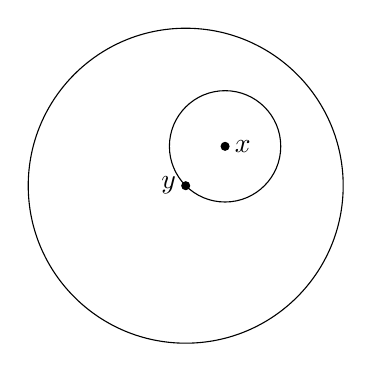
\begin{tikzpicture}
        \filldraw (0.5, 0.5) circle (0.05) node[right] {$x$};
        \draw (0.5, 0.5) circle (0.707);

        \filldraw (0, 0) circle (0.05) node[left] {$y$};
        \draw (0, 0) circle (2);
      \end{tikzpicture}
      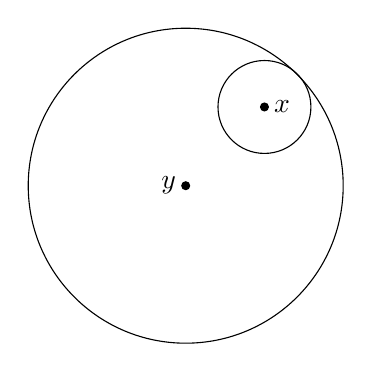
\begin{tikzpicture}
        \filldraw (1, 1) circle (0.05) node[right] {$x$};
        \draw (1, 1) circle (0.59);

        \filldraw (0, 0) circle (0.05) node[left] {$y$};
        \draw (0, 0) circle (2);
      \end{tikzpicture}
    \end{center}
  \end{description}
\end{proof}

\begin{proposition}\label{thm:locally_countable_metric_topology}
  The following is an alternative base for the metric topology\Tinyref{def:metric_topology}:

  \begin{align*}
    \Cal{B}(x) \coloneqq \{ B (x, \tfrac 1 n) \colon n = 1, 2, 3, \ldots \}.
  \end{align*}
\end{proposition}
\begin{proof}
  The proof is the same as in \cref{def:metric_topology}, except for a slight tweak in \ref{thm:topological_local_base_axioms/BP3}, where we define $m$ to be the the smallest positive integer such that
  \begin{align*}
    \tfrac 1 m \leq \min\{ \mu(x, y), r - \mu(x, y) \}.
  \end{align*}

  Note that $m$ exists by \cref{thm:ordinals_are_well_ordered}.

  We then obtain $B(x, \tfrac 1 m) \subseteq B(y, \tfrac 1 n)$.
\end{proof}

\begin{proposition}\label{thm:metric_topology_properties}
  The metric topology $\Cal{T}$ on $X$ induced by $\mu$ has the following properties:
  \begin{defenum}
    \item\label{thm:metric_topology_properties/ball_is_open} For every point $x \in X$ and any radius $r > 0$, the ball $B(x, r)$ is an open set and, hence, a neighborhood of $x$.
    \item\label{thm:metric_topology_properties/first_countable} $\Cal{T}$ is first-countable.
    \item\label{thm:metric_topology_properties/hausdorff} $\Cal{T}$ is Hausdorff.
  \end{defenum}
\end{proposition}
\begin{proof}
  \begin{description}
    \item[\ref{thm:metric_topology_properties/ball_is_open}] Obvious from \cref{def:metric_topology}.

    \item[\ref{thm:metric_topology_properties/first_countable}] Since \cref{thm:locally_countable_metric_topology} involves generating a topology using a neighborhood system of countable local neighborhoods, $\Cal{T}$ is first-countable.

    \item[\ref{thm:metric_topology_properties/hausdorff}] $\Cal{T}$ is Hausdorff by \cref{thm:t2_iff_singleton_limits} since a net.
  \end{description}
\end{proof}

\begin{proposition}\label{thm:metric_convergence_iff_metric_topology_convergence}
  Let $(X, \mu)$ be a metric space and $\Cal{T}$ be the induced metric topology\Tinyref{def:metric_topology}. The convergence\Tinyref{sec:convergence} in $\Cal{T}$ is the completely described by sequences.

  Fix a sequence $\{ x_i \}_{i=1}^\infty$ and consider the sequence as a net\Tinyref{def:topological_net}. Then
  \begin{defenum}
    \item\label{thm:metric_convergence_iff_metric_topology_convergence/cluster_point} $x \in X$ is a cluster point\Tinyref{def:net_cluster_point} of the sequence $\{ x_i \}_{i=1}^\infty$ if and only if for every positive real number $\varepsilon > 0$ and every index $i_0$ there exists an index $i_\varepsilon > i_0$ such that
    \begin{align*}
      \mu(x, x_{i_\varepsilon}) < \varepsilon.
    \end{align*}

    \item\label{thm:metric_convergence_iff_metric_topology_convergence/limit_point} $x \in X$ is a limit point\Tinyref{def:net_limit_point} of the sequence $\{ x_i \}_{i=1}^\infty$ if and only if for every positive real number $\varepsilon > 0$ there exists an index $i_0$ such that
    \begin{align*}
      i \geq i_0 \implies \mu(x, x_i) < \varepsilon.
    \end{align*}

    \item\label{thm:metric_convergence_iff_metric_topology_convergence/closure} Fix a set $A \subseteq X$. A point $x \in X$ belongs to $\Cl{A}$ if and only if there exists a sequence $\{ x_i \}_{i=1}^\infty \subseteq A$ such that $x_i \xrightarrow[i \to \infty]{} x$ (compare with \cref{thm:limit_point_iff_in_closure}).
  \end{defenum}
\end{proposition}
\begin{proof}
  \begin{description}
    \item[\ref{thm:metric_convergence_iff_metric_topology_convergence/cluster_point}] Fix a sequence $x_i \to x$.

    \Implies Fix a radius $\varepsilon > 0$ and an index $i_0$. Note that $B(x, \varepsilon)$ is a neighborhood of $x$ and hence by \cref{def:net_cluster_point} there exists an index $i_\varepsilon \geq i_0$ such that $x_{i_U} \in B(x, \varepsilon)$, which is the same as
    \begin{align*}
      \mu(x, x_{i_U}) < \varepsilon.
    \end{align*}

    \ImpliedBy Fix a neighborhood $U$ of $x$. Since the topology is generated by a local base of balls, then $U$ contains some ball $B(x, r)$. Thus there exists an index $i_0$, such that
    \begin{align*}
      \mu(x, x_{i_r}) < r,
    \end{align*}
    hence
    \begin{align*}
      x_{i_r} \in B(x, r) \subseteq U.
    \end{align*}

    \item[\ref{thm:metric_convergence_iff_metric_topology_convergence/limit_point}] Similar to \ref{thm:metric_convergence_iff_metric_topology_convergence/cluster_point}.

    \item[\ref{thm:metric_convergence_iff_metric_topology_convergence/closure}]
    \Implies Fix a nonempty set $A$ and $x \in \Cl A$. If $x \in A$, then the constant sequence with all members equal to $x$ converges to $A$.

    Assume that $x \not\in A$ and choose any sequence\AOC
    \begin{align*}
      x_i \in B(x, \tfrac 1 i) \setminus \{ x \}, i = 1, 2, \ldots.
    \end{align*}

    Fix $\varepsilon > 0$. By \cref{thm:ordinals_are_well_ordered} there exists a least positive integer $i_0$ such that $\tfrac 1 i_0 < \varepsilon$. It follows that $x_i \to x$ since
    \begin{align*}
      i \geq i_0 \implies \mu(x, x_i) \leq \mu(x, x_{i_0}) \leq \varepsilon.
    \end{align*}

    \ImpliedBy Obvious
  \end{description}
\end{proof}

  \section{Metric spaces}\label{sec:metric_spaces}
\subsection{Metric spaces}\label{subsec:metric_spaces}

\begin{definition}\label{def:metric_space}\MarginCite[248]{Engelking1989}
  A \Def{metric space} is a set \( X \) along with a nonnegative real-valued function \( \rho: X \times X \to [0, \infty) \), called a \Def{metric}, also called the \Def{distance function}, such that
  \begin{DefEnum}[series=def:metric_space]
    \IAxiom{def:metric_space/M1}{M1} \( \rho(x, y) = 0 \iff x = y \)
    \IAxiom{def:metric_space/M2}{M2}(symmetry) \( \rho(x, y) = \rho(y, x) \)
    \IAxiom{def:metric_space/M3}{M3}(triangle inequality) \( \rho(x, y) \leq \rho(x, z) + \rho(z, y) \)
  \end{DefEnum}

  If instead of \ref{def:metric_space/M1} we have the weaker condition
  \begin{DefEnum}[resume=def:metric_space]
    \IAxiom{def:metric_space/pseudometric_identity}{M1'} \( \forall x \in X, \rho(x, x) = 0 \),
  \end{DefEnum}
  we call \( \rho \) a \Def{pseudometric} and \( (X, \rho) \) a \Def{pseudometric space}.

  \begin{DefEnum}
    \ILabel{def:metric_space/subspace} If \( A \subseteq X \) is a set, then the restriction \( (A, \rho{\restriction_A}) \) is a metric space and it is called a \Def{subspace} of $X$.

    \ILabel{def:metric_space/ball} Define the function
    \begin{BreakableAlign*}
       & B: X \times (0, \infty) \to \Pow(X),                   \\
       & B(x, r) \coloneqq \{ y \in X \colon \rho(x, y) < r \}.
    \end{BreakableAlign*}

    The set \( B(x, r) \) is called an \Def{open ball} or simply \Def{ball} with \Def{center} \( x \) and \Def{radius} \( r \).

    The ball \( B = B(0, 1) \) is called the \Def{unit ball}.

    \ILabel{def:metric_space/closed_ball} The set
    \begin{equation*}
      \Ol{B(x, r)} \coloneqq \Cl(B(x, r))
    \end{equation*}
    is called the \Def{closed ball} with center \( x \) and radius \( r \).

    \ILabel{def:metric_space/sphere} The set
    \begin{equation*}
      S(x, r) \coloneqq \Bd{B(x, r)}
    \end{equation*}
    is called the \Def{sphere} with center \( x \) and radius \( r \).

    \ILabel{def:metric_space/bounded_set} A set \( A \subseteq X \) is called \Def{bounded} if it is contained in some ball \( B(x, r) \).

    \ILabel{def:metric_space/bounded_sequence} A \hyperref[def:sequence]{sequence} \( \{ x_k \}_{k=1}^\infty \subseteq X \) is called \Def{bounded} if the corresponding set \( \{ x_k \colon k = 1, 2, \ldots \} \) is \hyperref[def:metric_space/bounded_set]{bounded}.

    \ILabel{def:metric_space/bounded_metric} If every set is bounded, we say that the metric itself is bounded.

    \ILabel{def:metric_space/bounded_function} We say that a function \( f: S \to X \) from a set \( S \) to a metric space \( (X, \rho) \) is \Def{bounded} if its image \( f(S) \) is a bounded set in \( (X, \rho) \).

    \ILabel{def:metric_space/diameter} Define the function
    \begin{BreakableAlign*}
       & \Diam: \Pow(X) \to [0, \infty],                             \\
       & \Diam(A) \coloneqq \sup \{ \rho(x, y) \colon x, y \in A \},
    \end{BreakableAlign*}
    whose values include the nonnegative extended real \hyperref[def:extended_real_numbers]{numbers}.

    If it exists, we call the number \( \Diam(A) \) the \Def{diameter of \( A \)}.

    \ILabel{def:metric_space/distance} Define the function
    \begin{BreakableAlign*}
       & \Dist: X \times \Pow(X) \to [0, \infty),                    \\
       & \Dist(x, A) \coloneqq \inf \{ \rho(x, a) \colon a \in A \}.
    \end{BreakableAlign*}

    We call the number \( \Dist(x, A) \) the \Def{distance from the point \( x \) to the set \( A \)}. We use the convention that the infimum of an empty set of real numbers is \( +\infty \), hence \( \Dist(x, \varnothing) = \infty \).
  \end{DefEnum}
\end{definition}

\begin{proposition}\label{thm:pseudometric_to_metric}
  Let \( (X, \rho) \) be a \hyperref[def:metric_space]{pseudometric space}. Define the equivalence relation
  \begin{equation*}
    x \cong y \iff \rho(x, y) = 0.
  \end{equation*}

  Then the following metric on the \hyperref[thm:equivalence_partition]{quotient set} \( M \coloneqq X / \cong \)
  \begin{BreakableAlign*}
     & \rho: M \times M \to [0, \infty)    \\
     & \rho([x], [y]) \coloneqq \rho(x, y)
  \end{BreakableAlign*}
  is well defined.
\end{proposition}
\begin{proof}
  The function \( \rho \) is well defined since, if \( x \) and \( y \) both belong to the same equivalence class \( [x] \), then \( \rho(x) = \rho(y) \). Thus \( \rho \) does not depend on the choice of representatives.

  Additionally, \( \rho \) is a metric since \( \rho([x], [y]) = 0 \) implies that \( [x] = [y] \), that is, \( \rho(x, y) = 0 \).
\end{proof}

\begin{proposition}\label{remark:bounded_set_metric_order_equivalence}
  A set \( A \) in a metric space \( (X, \rho) \) is \hyperref[def:metric_space/bounded_set]{bounded} if and only if the set \( \{ \rho(a, b) \colon a, b \in A \} \) is bounded as a \hyperref[def:preordered_set/bounded_set]{poset}.
\end{proposition}

\begin{definition}\label{def:metric_topology}\MarginCite[249]{Engelking1989}
  Let \( (X, \rho) \) be a metric space. We define the \Def{metric topology}\( \CT \) , also called the \Def{induced topology}, as the \hyperref[def:topological_space]{topology} generated by the \hyperref[def:topological_local_base]{neighborhood system}
  \begin{equation}\label{def:metric_topology/integer_base}
    \Cal{B}(x) \coloneqq \{ B(x, \tfrac 1 n) \colon n = 1, 2, 3, \ldots \}.
  \end{equation}

  If for some topological space \( (X, \CT) \) there exists a metric such that \( \CT \) is its induced topology, we say that the topology \( \CT \) is \Def{metrizable}.

  It is often conventional to consider the alternative (larger) base
  \begin{equation}\label{def:metric_topology/real_base}
    \Cal{B}'(x) \coloneqq \{ B(x, \varepsilon) \colon \varepsilon > 0 \}.
  \end{equation}
\end{definition}
\begin{proof}
  This is indeed a neighborhood system as it satisfies \fullref{thm:topological_local_base_axioms/BP1}-\fullref{thm:topological_local_base_axioms/BP3}:

  \begin{RefList}
    \IRef{thm:topological_local_base_axioms/BP1} Every point \( x \) belongs to any ball centered at \( x \).

    \IRef{thm:topological_local_base_axioms/BP2} Fix \( x \in X \) and two balls \( B(x, \tfrac 1 n) \) and \( B(x, \tfrac 1 m) \). Then
    \begin{equation*}
      B(x, \tfrac 1 {\max\{ n, m \}}) \subseteq B(x, n) \cap B(x, m).
    \end{equation*}

    \IRef{thm:topological_local_base_axioms/BP3} Fix \( x, y \in X \) and let \( x \in B(y, \tfrac 1 n) \), i.e. \( \rho(x, y) < \tfrac 1 n \).

    \begin{figure}
      \centering
      \begin{mplibcode}
        u := 1cm;
        r := sqrt(2) / 2;

        pair v;
        v := (1, 1);

        beginfig(1);
        draw fullcircle scaled 3u;
        dotlabel.bot("$y$", origin);

        draw fullcircle scaled 1u shifted (-r * u * v);
        dotlabel.bot("$x_1$", -r * u * v);

        draw fullcircle scaled 1u shifted (r/2 * u * v);
        dotlabel.bot("$x_2$", r/2 * u * v);
        endfig;
      \end{mplibcode}
      \Caption{def:metric_topology/nested_balls}{There is a nested ball around every point in an open ball}
    \end{figure}

    Define \( m \) to be the the smallest positive integer such that
    \begin{equation*}
      \tfrac 1 m \leq \min\{ \rho(x, \tfrac 1 n), \tfrac 1 n - \rho(x, \tfrac 1 n) \}.
    \end{equation*}

    Note that \( m \) exists by \fullref{thm:ordinals_are_well_ordered}.

    Let \( z \in B(x, \tfrac 1 m) \). There are two cases:
    \begin{itemize}
      \item If \( \rho(x, y) \leq \tfrac 1 {2n} \), then
            \begin{BreakableAlign*}
              \rho(z, y)
              \leq
              \rho(z, x) + \rho(x, y)
              <
              \tfrac 1 m + \rho(x, y)
              \leq
              \tfrac 1 n + \tfrac 1 n
              \leq
              2 \tfrac 1 {2n}
              =
              \tfrac 1 n.
            \end{BreakableAlign*}

      \item If \( \rho(x, y) > \tfrac 1 {2n} \), then
            \begin{BreakableAlign*}
              \rho(z, y)
              \leq
              \rho(z, x) + \rho(x, y)
              <
              \tfrac 1 m + \rho(x, y)
              \leq
              (\tfrac 1 n - \rho(x, y)) + \rho(x, y)
              =
              \tfrac 1 n.
            \end{BreakableAlign*}
    \end{itemize}

    In both cases, \( B(x, \tfrac 1 m) \subseteq B(y, \tfrac 1 n) \).
  \end{RefList}
\end{proof}

\begin{proposition}\label{thm:metric_topology_properties}
  The metric topology \( \CT \) on \( X \) induced by \( \rho \) has the following properties:
  \begin{DefEnum}
    \ILabel{thm:metric_topology_properties/ball_is_open} For every point \( x \in X \) and any radius \( r > 0 \), the ball \( B(x, r) \) is an open set and, hence, a neighborhood of \( x \).
    \ILabel{thm:metric_topology_properties/first_countable} \( \CT \) is first-countable.
    \ILabel{thm:metric_topology_properties/sequential} \( \CT \) is sequential.
    \ILabel{thm:metric_topology_properties/hausdorff} \( \CT \) is Hausdorff.
  \end{DefEnum}
\end{proposition}
\begin{proof}
  \SubProofOf{thm:metric_topology_properties/ball_is_open} Obvious from \fullref{def:metric_topology}.

  \SubProofOf{thm:metric_topology_properties/first_countable} Since \fullref{def:metric_topology} involves generating a topology using a neighborhood system of countable local neighborhoods, \( \CT \) is first-countable.

  \SubProofOf{thm:metric_topology_properties/sequential} Follows from \fullref{thm:metric_topology_properties/first_countable} and \fullref{thm:first_countable_spaces_are_sequential}.

  \SubProofOf{thm:metric_topology_properties/hausdorff} Let \( x, y \in X \) be distinct points. Define
  \begin{equation*}
    r \coloneqq \dfrac 1 2 \rho(x, y),
  \end{equation*}
  so that
  \begin{equation*}
    B(x, r) \cap B(y, r) = \varnothing.
  \end{equation*}
\end{proof}

\begin{definition}\label{def:metric_uniformity}
  Let \( (X, \rho) \) be a metric space.

  We define the \Def{metric uniformity} \( \CV \), also called the \Def{induced uniformity}, as the \hyperref[def:uniform_space]{uniformity} generated by the countable \hyperref[thm:uniform_space_base_axioms]{base}
  \begin{equation}\label{def:metric_uniformity/integer_base}
    \Cal{B} \coloneqq \{ V_n \colon n = 1, 2, \ldots \},
  \end{equation}
  where
  \begin{equation*}
    V_n \coloneqq \rho^{-1}([0, \tfrac 1 n)).
  \end{equation*}

  As for the \hyperref[def:metric_topology]{metric topology}, we can instead consider the base
  \begin{equation}\label{def:metric_uniformity/real_base}
    \Cal{B}' \coloneqq \{ \rho^{-1}([0, \varepsilon)) \colon \varepsilon > 0 \}.
  \end{equation}
\end{definition}
\begin{proof}
  Each relation \( V_r \) is obviously an entourage by \ref{def:metric_space/M1} and \ref{def:metric_space/M2}. We will prove that \( \Cal{B} \) is indeed a uniform space base.

  \begin{RefList}
    \IRef{thm:uniform_space_base_axioms/BU1} For nonnegative integers \( n, m \) we have
    \begin{equation*}
      V_n \cap V_m
      =
      \{ (x, y) \in X \times X \colon \rho(x, y) < \tfrac 1 n \Tand \rho(x, y) < \tfrac 1 m \}
      =
      V_{\max\{ n, m \}}.
    \end{equation*}

    Pick any integer \( k \geq \max\{ n, m \} \) so that
    \begin{equation*}
      V_k \subseteq V_n \cap V_m.
    \end{equation*}

    \IRef{thm:uniform_space_base_axioms/BU2} Fix \( V_n \in \CV \) and \( m \coloneqq 2n \). By the triangle inequality, we have that if \( \rho(x, y) < m \) and \( \rho(y, z) < m \), then
    \begin{equation*}
      \rho(x, z) \leq \rho(x, y) + \rho(y, z) < \tfrac 1 m + \tfrac 1 m = \tfrac 1 n.
    \end{equation*}

    Thus
    \begin{equation*}
      V_m + V_m
      =
      \left\{ (x, z) \colon \exists y \in X: \rho(x, y) < \tfrac 1 m \Tand \rho(y, z) < \tfrac 1 m \right\}
      \subseteq
      V_n
    \end{equation*}

    \IRef{thm:uniform_space_base_axioms/BU3} \ref{def:metric_space/M1} implies that
    \begin{equation*}
      \bigcap \CB = \lim_{n \to \infty} \rho^{-1}([0, \tfrac 1 n)) = \Delta_X.
    \end{equation*}
  \end{RefList}
\end{proof}

\begin{proposition}\label{thm:metric_topology_coincides_with_uniform_topology}
  The \hyperref[def:metric_topology]{metric topology} and the \hyperref[def:uniform_topology]{uniform topology} from the \hyperref[def:metric_uniformity]{metric uniformity} coincide.
\end{proposition}

\begin{theorem}\label{thm:countable_uniform_base_implies_metrizable}\MarginCite[thm. 8.1.21]{Engelking1989}
  A uniform space \( X \) is metrizable if and only \( w(X) \leq \aleph_0 \).
\end{theorem}

\medskip

\begin{definition}\label{def:isometry}\MarginCite[253]{Engelking1989}
  Let \( (X, \rho) \) and \( (Y, \nu) \) be two \hyperref[def:metric_space]{metric spaces}. We say that the function \( f: X \to Y \) is a \Def{distance preserving map} or \Def{isometry} or \Def{isometric embedding} if
  \begin{equation*}
    \forall x, y \in X, \rho(x, y) = \nu(f(x), f(y)).
  \end{equation*}

  If \( f \) is bijective, we say that \( X \) and \( Y \) are \Def{isometric}.
\end{definition}

\begin{proposition}\label{thm:isometry_is_injective}
  An \hyperref[def:isometry]{isometry} \( f: (X, \rho) \to (Y, \nu) \) is always injective.
\end{proposition}
\begin{proof}
  If\LEM \( f(x) = f(x') \), then by \fullref{def:metric_space/M1}, \( x = x' \).
\end{proof}

\begin{definition}\label{def:category_of_metric_spaces}
  Metric spaces and monotone maps form a subcategory of \( \Cat{Unif} \) (see \fullref{def:category_of_uniform_spaces}). We denote this category by \( \Cat{Met} \).
\end{definition}

\begin{definition}\label{def:equivalent_metrics}
  Two metrics \( \rho \) and \( \nu \) on the set \( X \) are said to be \Def{equivalent} if \( \rho \) and \( \nu \) have the same \hyperref[def:metric_topology]{metric topology}. They are said to be \Def{strongly equivalent} if there exist constants \( \alpha, \beta \in \BR \) such that for every \( x, y \in X \) we have
  \begin{equation*}
    \alpha \nu(x, y) \leq \rho(x, y) \leq \beta \nu(x, y).
  \end{equation*}
\end{definition}

\begin{remark}\label{remark:metric_space_convergence}
  All types of convergence from \fullref{subsec:topological_nets}, \fullref{subsec:topological_continuity} and \fullref{subsec:uniform_spaces} hold in metric spaces using the \hyperref[def:metric_topology]{metric topology} and \hyperref[def:metric_uniformity]{metric uniformity} structure.

  It is conventional to prefer the bases \fullref{def:metric_topology/real_base} and \fullref{def:metric_uniformity/real_base} to the bases \fullref{def:metric_topology/integer_base} and \fullref{def:metric_topology/integer_base}.

  For example, given two metric spaces \( X \) and \( Y \), continuity of \( f: X \to Y \) at \( x_0 \in X \) (see \fullref{def:local_continuity}) is usually written using the \enquote{epsilon-delta notation} as
  \begin{equation*}
    \forall \varepsilon > 0 \ \exists \delta > 0 : \rho_X(x, x_0) < \delta \implies \rho_Y(f(x), f(x_0)) < \varepsilon
  \end{equation*}
  for any \( x \in X \).
\end{remark}

\begin{definition}\label{def:translation_invariant_metric}
  A \hyperref[def:metric_space]{metric} \( \rho \) on a \hyperref[def:group/magma]{magma} \( G \) is said to be \Def{left translation-invariant} if
  \begin{equation*}
    \rho(ax, ay) = \rho(x, y) \quad\forall a, x, y \in G
  \end{equation*}
  and \Def{right translation-invariant} if
  \begin{equation*}
    \rho(xa, ya) = \rho(x, y) \quad\forall a, x, y \in G.
  \end{equation*}

  If \( \rho \) is both left and right translation invariant (e.g. for commutative magmas), we simply say that \( \rho \) is \Def{translation invariant}.
\end{definition}

  \subsection{Complete metric spaces}\label{subsec:metric_convergence}

\begin{definition}\label{def:complete_metric_space}
  A metric space is said to be \term{complete} if
  \begin{thmenum}
    \thmitem{def:complete_metric_space/sequences} Every fundamental sequence converges.
    \thmitem{def:complete_metric_space/uniform} It is complete as a uniform space in the sense of \fullref{def:complete_uniform_space}
  \end{thmenum}
\end{definition}
\begin{proof}
  The equivalence is due to \fullref{thm:metric_topology_properties/sequential} and \fullref{thm:metric_topology_properties/hausdorff}.
\end{proof}

\begin{proposition}\label{thm:fundamental_sequence_is_bounded}
  In a metric space, any \hyperref[def:fundamental_net]{fundamental sequence} \( \{ x_k \}_{i=1}^n \) is \hyperref[def:metric_space/bounded_sequence]{bounded}.
\end{proposition}
\begin{proof}
  Since the set
  \begin{equation*}
    I \coloneqq \{ x_k \colon k \leq k_0 \}
  \end{equation*}
  is finite, it has a finite \hyperref[def:metric_space/diameter]{diameter}.

  Fix \( \varepsilon > 0 \). Since the sequence is fundamental, there exists an index \( k_0 \) such that
  \begin{equation*}
    \rho(x_k, x_m) < \varepsilon \quad\forall k, m \geq k_0.
  \end{equation*}

  We are only interested in the case \( \rho(x_{k_0}, x_m) < \varepsilon \).

  Let \( k < k_0 \) and \( m \geq k_0 \). Then
  \begin{equation*}
    \rho(x_k, x_m) \leq \rho(x_k, x_{k_0}) + \rho(x_{k_0}, x_m) < \diam(I) + \varepsilon,
  \end{equation*}
  which is a finite number.

  Thus, the distance between any two elements of the sequence is finite and the sequence is bounded.
\end{proof}

\begin{proposition}\label{thm:fundamental_subsequence_convergence}
  In any \hyperref[def:complete_metric_space]{metric space}, a \hyperref[def:fundamental_net]{fundamental sequence} converges to a value if and only if it has a subsequence that converges to the same value.
\end{proposition}
\begin{proof}
  Let \( (X, \rho) \) be a metric space and let \( \{ x_k \}_{k=1}^\infty \) be a fundamental sequence.

  \SufficiencySubProof Obvious
  \NecessitySubProof Assume that the subsequence \( \{ x_{k_n} \}_{n=1}^\infty \) converges to \( x \). Fix \( \varepsilon > 0 \). There exist \( k_0 \) and \( n_0 \) such that
  \begin{balign*}
     & \rho(x_k, x_m) < \tfrac \varepsilon 2 \quad\forall k, m \geq k_0
     & \rho(x, x_{k_n}) < \tfrac \varepsilon 2 \quad\forall n \geq n_0.
  \end{balign*}

  Fix \( k \geq k_0 \) and let \( n \geq n_0 \) be such that \( k_n \geq k_0 \). Then
  \begin{equation*}
    \rho(x, x_k) \leq \rho(x, x_{k_n}) + \rho(x_{k_n}, x_k) < \varepsilon.
  \end{equation*}

  Since \( \varepsilon \) was arbitrary, we conclude that \( \lim_{k \to \infty} x_k = \lim_{n \to \infty} x_{k_n} = x \).
\end{proof}

\begin{lemma}\label{thm:metric_space_completion_uniqueness}
  Let \( X \) be a metric space. If both \( f: X \to Y \) and \( g: X \to Z \) are \hyperref[def:complete_metric_space]{completions} of \( X \), then \( Y \) and \( Z \) are isometric.
\end{lemma}
\begin{proof}
  Let \( y \in Y \) and let \( \{ x_k \}_{k \to \infty} \subseteq X \) be a sequence such that
  \begin{equation*}
    f(x_k) \xrightarrow[k \to \infty]{} y.
  \end{equation*}

  Such a sequence exists since \( f(X) \) is dense in \( Y \).

  Define \( z \coloneqq \lim_{k \to \infty} g(x_k) \). Since both \( f \) and \( g \) are isometries, \( z \) does not depend on the choice of sequence \( \{ x_k \}_{k \to \infty} \) such that \( f(x_k) \to y \). Furthermore, if \( z \in Z \) is given rather than \( y \in Y \), an analogous process allows us to determine \( y \) uniquely based on \( z \).

  Thus, we have a bijective isometry between \( Y \) and \( Z \).
\end{proof}

\begin{theorem}[Metric space completion]\label{thm:metric_space_completion}
  Every metric space has a unique (up to an isometry) \hyperref[def:complete_metric_space]{completion}.

  This is a special case of \fullref{thm:uniform_space_completion} that we prove fully.
\end{theorem}
\begin{proof}
  Let \( (X, \rho) \) be a metric space. Uniqueness of the completion follows from \fullref{thm:metric_space_completion_uniqueness}. We will only show existence.

  \begin{thmenum}
    \thmitem{thm:metric_space_completion/part_a} First, we build the pseudometric space \( (F, \rho) \). We deal with fundamental sequences and isometries in pseudometric spaces, where the definitions, however, does not change.

    Define \( F \) to be the set of all fundamental \hyperref[def:fundamental_net]{sequences} in X. Define the pseudometric
    \begin{balign*}
       & \rho: F \times F \to \BbbR_{\geq 0}                                                                               \\
       & \rho\left( \{ x_k \}_{k=1}^\infty, \{ y_k \}_{k=1}^\infty \right) \coloneqq \lim_{k \to \infty} \rho(x_k, y_k).
    \end{balign*}

    We first show that is well-defined as a \hyperref[def:function]{function}. Let \( \{ x_k \}_{k=1}^\infty \) and \( \{ y_k \}_{k=1}^\infty \) be two sequences. Fix \( \varepsilon > 0 \). Then there exists an \( k_0 \) such that
    \begin{equation*}
      \rho(x_k, x_k) < \tfrac \varepsilon 2 \text{ and } \rho(y_k, y_m) <  \quad\forall k, m \geq k_0.tfrac \varepsilon 2.
    \end{equation*}

    Fix \( k, m \geq k_0 \). Then
    \begin{equation*}
      \rho(x_k, y_k) \leq \rho(x_k, x_m) + \rho(x_m, y_m) + \rho(y_m, y_k) < \rho(x_m, y_m) + \varepsilon,
    \end{equation*}
    hence
    \begin{equation*}
      \abs{\rho(x_k, y_k) - \rho(x_m, y_m)} < \varepsilon.
    \end{equation*}

    Thus, the sequence \( \{ \rho(x_k, y_k) \}_{k=1}^\infty \) is fundamental and, by \fullref{def:real_numbers_complete_metric_space}, it is convergent.

    Now we check that \( \rho \) is indeed a pseudometric:
    \SubProofOf{def:metric_space/pseudometric_identity} For every sequence \( x \in F \),
    \begin{equation*}
      \rho(x, x) = \lim_{k \to \infty} \rho(x_k, x_k) = 0.
    \end{equation*}
    \SubProofOf{def:metric_space/M2} For all sequences \( x, y \in F \),
    \begin{equation*}
      \rho(x, y) = \lim_{k \to \infty} \rho(x_k, y_k) = \lim_{k \to \infty} \rho(y_k, x_k) = \rho(y, x).
    \end{equation*}

    \SubProofOf{def:metric_space/M3} For all sequences \( x, y, z \in F \),
    \begin{equation*}
      \rho(x, z) = \lim_{k \to \infty} \rho(x_k, z_i) \leq \lim_{k \to \infty} \rho(x_k, y_k) + \lim_{k \to \infty} \rho(y_k, z_i) = \rho(x, y) + \rho(y, z).
    \end{equation*}

    \thmitem{thm:metric_space_completion/part_b} We prove that every fundamental sequence in \( (F, \rho) \) is convergent.

    Let \( \{ c^{(k)} \}_{k=1}^\infty \) be a fundamental sequence (of sequences) in \( (F, \rho) \). Thus, for every \( k = 1, 2, \ldots \), there exists an index \( n_k \) such that
    \begin{equation*}
      \rho(c_m^{(k)}, c_{n_k}^{(k)}) < \tfrac 1 k \quad\forall m \geq n_k.
    \end{equation*}

    Define the sequence
    \begin{equation*}
      d_k \coloneqq c_{n_k}^{(k)}, k = 1, 2, \ldots.
    \end{equation*}

    To see that it is fundamental, fix \( \varepsilon > 0 \). Now since the sequence \( \{ c^{(k)} \} \) in \( F \) is fundamental, there exists \( k_0 \) such that
    \begin{equation*}
      \rho(c^{(k)}, c^{(m)}) = \lim_{k \to \infty} \rho(c_k^{(k)}, c_k^{(m)}) < \frac \varepsilon 2 \quad\forall k, m \geq k_0.
    \end{equation*}

    Let \( m_0 \geq k_0 \) be an index such that
    \begin{equation*}
      \frac 2 {m_0} < \frac \varepsilon 2.
    \end{equation*}

    Fix \( k \geq m \geq m_0 \). Let \( l \geq \max \{ n_k, n_m \} \) be such that
    \begin{equation*}
      \rho(c_l^{(k)}, c_l^{(m)}) < \frac \varepsilon 2.
    \end{equation*}

    Then
    \begin{balign*}
      \rho(d_k, d_m)
       & =
      \rho(c_{n_k}^{(k)}, c_{n_m}^{(m)})
      \leq \\ &\leq
      \rho(c_{n_k}^{(k)}, c_l^{(k)}) + \rho(c_l^{(k)}, c_l^{(m)}) + \rho(c_l^{(m)}, c_{n_m}^{(m)})
      \leq \\ &\leq
      \frac 1 k + \frac \varepsilon 2 + \frac 1 m
      \leq
      \frac 2 m + \frac \varepsilon 2
      <
      \varepsilon.
    \end{balign*}

    Thus, we have
    \begin{equation*}
      \rho(d_k, d_m) < \varepsilon \quad\forall k \geq m \geq m_0,
    \end{equation*}
    which proves that the sequence \( \{ d_k \}_{k=1}^\infty \) is fundamental in \( (X, \rho) \).

    Now it remains to show that \( c^{(k)} \xrightarrow[k \to \infty]{} d \) in \( (F, \rho) \).

    Fix \( \varepsilon > 0 \) and let \( k_0 \) be such that
    \begin{equation*}
      \frac 1 {k_0} \leq \frac \varepsilon 2.
    \end{equation*}
    and
    \begin{equation*}
      \rho(d_k, d_m) < \frac \varepsilon 2 \quad\forall k, m \geq k_0.
    \end{equation*}

    Now fix \( i \geq k_0 \). We have, for all \( k \geq i \),
    \begin{balign*}
      \rho(c_{n_k}^{(k)}, d_k)
       & =
      \rho(c_{n_k}^{(k)}, c_{n_k}^{(k)})
      \leq \\ &\leq
      \rho(c_{n_k}^{(k)}, c_{n_k}^{(k)}) + \rho(c_{n_k}^{(k)}, c_{n_k}^{(k)})
      =    \\ &=
      \rho(c_{n_k}^{(k)}, c_{n_k}^{(k)}) + \rho(d_k, d_k)
      <    \\ &<
      \frac 1 k + \frac \varepsilon 2
      <
      \varepsilon.
    \end{balign*}

    Hence,
    \begin{balign*}
      \rho(c^{(k)}, d)
      =
      \lim_{k \to \infty} \rho(c_k^{(k)}, d_k)
      =
      \lim_{k \to \infty} \rho(c_k^{(k)}, c_{n_k}^{(k)})
      <
      \varepsilon.
    \end{balign*}

    Thus, given \( \varepsilon > 0 \), we found an index \( k_0 \) such that
    \begin{equation*}
      \rho(c^{(k)}, d) < \varepsilon \quad\forall g \geq k_0.
    \end{equation*}

    Thus, \( d = \lim_{k \to \infty} c^{(k)} \) and \( (F, \rho) \) is a complete pseudometric space.

    \thmitem{thm:metric_space_completion/part_c} We construct an isometry of \( (X, \rho) \) into \( (F, \rho) \).

    Define the function
    \begin{balign*}
       & \iota: X \to F                        \\
       & \iota(x) \coloneqq (x, x, x, \ldots),
    \end{balign*}
    which sends each element of \( X \) into the corresponding constant sequence in \( F \).

    It is an \hyperref[def:isometry]{isometry} since
    \begin{equation*}
      \rho(\iota(x),\iota(y)) = \lim_{k \to \infty} \rho(x, y) = \rho(x, y).
    \end{equation*}

    \thmitem{thm:metric_space_completion/part_d} We show that the image \( \iota(X) \) is dense in \( (F, \rho) \).

    Fix the fundamental sequence \( y \coloneqq \{ y_k \}_{k=1}^\infty \). Define the sequence \( x \) of sequences
    \begin{equation*}
      x^{(k)} \coloneqq \iota(y_k), i = 1, 2, \ldots.
    \end{equation*}

    It is fundamental in \( (F, \rho) \) since \( e \) is an isometry and since \( y \) is fundamental in \( (X, \rho) \).

    Fix \( \varepsilon > 0 \). Let \( k_0 \) be such that
    \begin{equation*}
      \rho(y_k, y_m) < \varepsilon \quad\forall k, m \geq k_0.
    \end{equation*}

    For \( i, k \geq k_0 \), we have
    \begin{balign*}
      \rho(x_k^{(k)}, y_k)
      \leq
      \rho(x_k^{(k)}, y_k) + \rho(y_k, y_k)
      =
      0 + \rho(y_k, y_k)
      <
      \varepsilon,
    \end{balign*}
    hence
    \begin{equation*}
      \rho(x^{(k)}, y) = \lim_{k \to \infty} \rho(x_k^{(k)}, y_k) < \varepsilon.
    \end{equation*}

    We conclude that \( x^{(k)} \xrightarrow[k \to \infty]{} y \) in \( (F, \rho) \), which implies that \( e(X) \) is dense in \( (F, \rho) \).

    \thmitem{thm:metric_space_completion/part_e} We build a complete metric space \( (C, \nu) \) from \( (F, \rho) \).

    We use \fullref{thm:pseudometric_to_metric} to construct a complete metric space \( (C, \nu) \) from the complete pseudometric space \( (F, \rho) \).

    We adapt \( \iota \) to the equivalence classes on \( C \):
    \begin{balign*}
       & \hat\iota: X \to C                 \\
       & \hat\iota(x) \coloneqq [\iota(x)].
    \end{balign*}

    Thus, \( \hat\iota \) embeds \( X \) into the complete metric space \( C \).
  \end{thmenum}
\end{proof}

\begin{theorem}[Cantor's nested compact theorem]\label{thm:cantors_nested_compact_theorem}
  A descending sequence of nonempty compact sets \( F_1 \supseteq F_2 \supseteq \ldots \) in a complete metric space such that \( \diam(F_i) \to 0 \) intersects at exactly one point (compare with \fullref{thm:noncompact_kuratowskis_lemma}).
\end{theorem}
\begin{proof}
  Choose an element \( x_k \in F_k \) for any \( i = 1, 2, \ldots \). Then the sequence \( \{ x_k \}_{k=1}^\infty \) is fundamental. To see this, let \( \varepsilon > 0 \) and let \( k_0 \) be an index such that \( \diam(F_{k_0}) < \varepsilon \). Then if \( j \geq i \geq k_0 \), \( x_m \) is contained in \( F_k \) and \( \rho(x_k, x_m) < \varepsilon \). Thus, the sequence is indeed fundamental and, since the space is complete, it has a limit point \( x \).

  The point \( x \) is contained in every set \( F_k, i = 1, 2, \ldots \) since all of the sets \( F_k \) are closed (by \fullref{thm:complete_metric_space_compact_conditions}) and contain their limit \hyperref[thm:limit_point_iff_in_closure]{points}. Thus,
  \begin{equation*}
    x \in \bigcap_{k=1}^\infty F_k.
  \end{equation*}

  Furthermore,
  \begin{equation*}
    \diam\left( \bigcap_{k=1}^\infty F_k \right) = 0,
  \end{equation*}
  hence \( x \) is the only point in the intersection.
\end{proof}

  Let $(X, \rho)$ be a metric space. Let $\B$ be the family of bounded sets in $X$.

  Let $(X, \rho)$ be a metric space. Let $\B$ be the family of bounded sets in $X$.

\begin{definition}\label{def:totally_bounded_set}
  The space $A \subseteq X$ is called \uline{totally bounded} if any of the following equivalent conditions hold:

  \begin{defenum}
    \item\label{def:totally_bounded_set/sets} For every $\varepsilon > 0$ there exists a finite cover of $A$ with sets with diameter at most $\varepsilon$.
    \item\label{def:totally_bounded_set/balls} For every $\varepsilon > 0$ there exists a finite cover of $A$ with balls of radius $\varepsilon$.
    \item\label{def:totally_bounded_set/zero_noncompactness/sets} Kuratowski's noncompactness measure (see~\cref{def:noncompactness_measures/sets}) $\alpha(A)$ is zero.
    \item\label{def:totally_bounded_set/zero_noncompactness/balls} The ball noncompactness measure (see~\cref{def:noncompactness_measures/balls}) $\beta(A)$ is zero.
    \item\label{def:totally_bounded_set/fundamental_subsequences} Every sequence in $A$ admits a fundamental subsequence.
  \end{defenum}

  Totally bounded sets are sometimes called \uline{precompact} (see \cref{def:compact_sets}) because of~\cref{thm:metric_sequentially_compact_iff_compact}. This equivalence requires the metric space to be complete, however.
\end{definition}
\begin{proof}
  The equivalences \ref{def:totally_bounded_set/sets} $\iff$ \ref{def:totally_bounded_set/zero_noncompactness/sets} and \ref{def:totally_bounded_set/balls} $\iff$ \ref{def:totally_bounded_set/zero_noncompactness/balls} are straightforward.

  (\ref{def:totally_bounded_set/balls} $\implies$ \ref{def:totally_bounded_set/sets}) Given $\varepsilon > 0$, any cover of $A$ with balls of radius $\frac \varepsilon 2$ is a cover with sets of diameter $\varepsilon$.

  (\ref{def:totally_bounded_set/sets} $\implies$ \ref{def:totally_bounded_set/balls}) Fix $\varepsilon > 0$ and $\mu \in (0, \varepsilon)$ and let $A_1, \ldots, A_n \subseteq \PS X$ be a finite cover of $A$ with sets of diameter at most $\mu$.

  Choose\AOC~a point $x_k$ from every $A_k$, $k = 1, \ldots, n$. We then have that for every $k = 1, \ldots, n$,
  \begin{align*}
    A_k \subseteq \Cl B(x_k, \mu) \subsetneq B(x_k, \varepsilon)
    \\
    \implies A \subseteq \bigcup_{k=1}^n A_k \subseteq \bigcup_{k=1}^n B(x_k, \mu) \subsetneq \bigcup_{k=1}^n B(x_k, \varepsilon),
  \end{align*}
  hence $x_1, \ldots, x_n$ are centers of $\varepsilon$-balls that cover $A$.

  (\ref{def:totally_bounded_set/balls} $\implies$ \ref{def:totally_bounded_set/fundamental_subsequences}) Let $\{ x_n \} \subseteq A$ be any sequence.

  If we assume\LEM\ that $\{ x_n \}$ has no fundamental subsequence, then there exists $\varepsilon_0 > 0$ such that $\rho(x_k, x_m) > \varepsilon_0$ for any $n, m \in \ZPos$.

  Consider a finite cover of $A$ with $\varepsilon_0$-balls. By the pigeonhole principle, at least one of the balls contains more than one element of the sequence, which contradicts the assumption that all elements of the sequence have a distance of at least $\varepsilon_0$.

  Hence an arbitrary sequence in $A$ has a fundamental subsequence.

  (\ref{def:totally_bounded_set/fundamental_subsequences} $\implies$ \ref{def:totally_bounded_set/balls}) Assume\LEM\ that there exists $\varepsilon_0 > 0$, such that $A$ admits no finite cover by $\varepsilon_0$-balls.

  Define $x_1 \in X, x_2 \in X \setminus B(x_1, \varepsilon_0), \ldots$, so that every two elements of the sequence $\{ x_n \}$ have a distance of at least $\varepsilon_0$. But then the sequence is does not admit a fundamental subsequence, which contradicts our assumption.

  This contradiction proves that $A$ admits a finite cover by $\varepsilon$-balls for every $\varepsilon > 0$.
\end{proof}

\begin{corollary}\label{thm:metric_compact_iff_closed_totally_bounded}
  Assume that $X$ is complete. The set $A \subseteq X$ is sequentially compact if and only if it is closed and totally bounded.
\end{corollary}
\begin{proof}
  The property that every sequence has a fundamental subsequence is equivalent to sequential compactness for a closed set in a complete metric space.
\end{proof}

\begin{proposition}\label{thm:closure_of_totally_bounded_is_totally_bounded}
  If a set $A \subseteq X$ is totally bounded, then so is its closure $\Cl A$.
\end{proposition}
\begin{proof}
  Let $\varepsilon > 0$ and $\mu \in (0, \varepsilon)$ and let $x_1, \ldots, x_n \in X$ be the centers of a cover of $A$ with $\mu$-balls.

  If $y$ is a point in $\Cl A \setminus A$, there exists a point $z \in A$ with $\rho(y, z) < \varepsilon - \mu$. Let $x_k \in A$ be one of the centers whose $\mu$-balls contain $z$. We then have that $y \in B(x_k, \varepsilon)$ since
  \begin{align*}
    \rho(x_k, z) \leq \rho(x_k, y) + \rho(y, z) < \mu + \varepsilon - \mu = \varepsilon.
  \end{align*}

  Hence the balls $\Cl B(x_k, \varepsilon)$ cover $\Cl A$, i.e.
  \begin{align*}
    \Cl A \subseteq \bigcup_{k=1}^n B(x_k, \varepsilon).
  \end{align*}
\end{proof}

\begin{lemma}[Lebesgue's covering lemma]\label{thm:lebesgue_covering_lemma}
  Assume that $X$ is complete. Let $A \subseteq X$ be sequentially compact. Given an open cover $\F \subseteq \PS A$, there exists a number $\delta > 0$ such that every $\delta$-ball with a center in $A$ is contained in some set of the cover $\F$.
\end{lemma}
\begin{proof}
  Assume\LEM\ that no such number $\delta > 0$ exists. Then for any natural number $n \in \ZPos$, there exists an element $x_n \in A$ such that the ball $B(x_n, \frac 1 n)$ is not contained in any set of the cover $\F$. Since $A$ is sequentially compact, the sequence $\{ x_n \}_n$ contains a convergent subsequence $\{ x_{n_k} \}_k$.

  Define
  \begin{align*}
    x \coloneqq \lim_{k \to \infty} x_{n_k}.
  \end{align*}

  Let\AOC\ $E$ be a set in $\F$ that contains $x$. Since $E$ is open, there exists some radius $r > 0$ such that $B(x, r) \subseteq E$.

  Choose any $k_0 > \frac 2 r$ such that $\rho(x_{n_{k_0}}, x) < \frac r 2$. By the triangle inequality,
  \begin{align*}
    B \left(x_{n_k}, \frac 1 k \right) \subsetneq B \left(x_k, \frac r 2 \right) \subseteq B(x, r) \subseteq E,
  \end{align*}
  which contradicts the choice of the sequence $\{ x_n \}_n$.

  Hence there exists a $\delta > 0$ such that for every $x \in A$, the ball $B(x, \delta)$ is contained in some element $E$ of the cover $\F$.
\end{proof}

\begin{theorem}\label{thm:metric_compact_iff_sequentially_compact}
  Assume that $X$ is complete. The set $A \subseteq X$ is compact if and only if it is sequentially compact
\end{theorem}
\begin{proof}
  ($\implies$) Let $\F \subseteq \PS X$ be an open cover of $A$.

  By the Lebesgue covering lemma (\cref{thm:lebesgue_covering_lemma}), there exists $\delta > 0$ such that for every $x \in A$, the ball $B(x, \delta)$ is contained in some set of the cover $\F$. Let $x_1, \ldots, x_n$ be a cover of $A$ with $\delta$-balls.

  For each $k = 1, \ldots, n$ we have that the ball $B(x_k, \delta)$ is contained in some set $E_k \in \F$. Hence $E_1, \ldots, E_n$ is a finite subcover of $A$, because
  \begin{align*}
    A \subseteq \bigcup_{k=1}^\infty B(x_k, \delta) \subseteq \bigcup_{k=1}^\infty E_k.
  \end{align*}

  Thus $A$ is compact.

  ($\impliedby$) Let $A$ be compact. Fix $\varepsilon > 0$ and take the cover
  \begin{align*}
    \F \coloneqq \{ B(a, \varepsilon) \colon a \in A \}.
  \end{align*}

  By compactness of $A$, there exists a finite subcover. Thus a finite cover of $A$ with $\varepsilon$-balls exists for every $\varepsilon > 0$. \Cref{def:totally_bounded_set} then implies that total boundedness is equivalent to sequential compactness because $X$ is complete and $A$ is closed.
\end{proof}

  \subsection{Noncompactness measures}\label{subsec:noncompactness_measures}

Let \( (X, \mu) \) be a metric space\Tinyref{def:metric_space}. Let \( \Cal{B} \) be the family of bounded sets\Tinyref{def:metric_space/bounded_set} in \( X \).

\begin{definition}\label{def:noncompactness_measures}\cite[definition 7.1]{Deimling1985}
  We define the following functions
  \begin{defenum}
    \DItem{def:noncompactness_measures/sets} The \textbf{Kuratowski measure of noncompactness},
    \begin{align*}
      &\alpha: \Cal{B} \to \BB{R}^{>0} \\
      &\alpha(A) \coloneqq \inf \{d > 0 \colon \exists U_1, \ldots, U_n \subseteq X: \Diam {U_k} < d \land A \subseteq \cup_{k=1}^n U_k \}
    \end{align*}

    \DItem{def:noncompactness_measures/balls} The \textbf{ball measure of noncompactness},
    \begin{align*}
      &\beta: \Cal{B} \to \BB{R}^{>0} \\
      &\beta(A) \coloneqq \inf \{r > 0 \colon \exists x_1, \ldots, x_2 \in X: A \subseteq \cup_{k=1}^n B(x_k, r) \}
    \end{align*}
  \end{defenum}
\end{definition}

\begin{example}\label{ex:noncompactness_measures}\cite[exercise 7.3]{Deimling1985}
  Consider the subsets \( A_2 \subseteq A_3 \subseteq A_1 \subseteq C([0, 1]) \), defined by
  \begin{align*}
    A_1 \coloneqq \left\{
      x \in C([0, 1]) \colon \begin{aligned}
        0 \leq t \leq 1 \implies 0 \leq x(t) \leq 1 \\
        x(0) = 0, x(1) = 1 \\
      \end{aligned}
    \right\}
    \\
    A_2 \coloneqq \left\{
      x \in A_1 \colon \begin{aligned}
        0 \leq t \leq \frac 1 2 \implies 0 \leq x(t) \leq \frac 1 2 \\
        \frac 1 2 \leq t \leq 1 \implies \frac 1 2 \leq x(t) \leq 1
      \end{aligned}
    \right\}
    \\
    A_3 \coloneqq \left\{
      x \in A_1 \colon \begin{aligned}
        0 \leq t \leq \frac 1 2 \implies 0 \leq x(t) \leq \frac 2 3 \\
        \frac 1 2 \leq t \leq 1 \implies \frac 1 3 \leq x(t) \leq 1
      \end{aligned}
    \right\}
  \end{align*}

  Then \( \alpha(A_1) = 1, \alpha(A_2) = \frac 1 2, \alpha(A_3) = \frac 1 3 \) and \( \beta(A_1) = \beta(A_2) = \beta(A_3) = \frac 1 2 \).
\end{example}
\begin{proof}
  Since the distance between any two functions from \( B_1 \) is at most 1, we have that \( \Diam B_1 = 1 \) and \( \alpha(B_1) \leq 1 \).

  Fix \( \varepsilon > 0 \). For any function \( f \in B_1 \), continuity of \( f \) gives us a radius \( \delta_f > 0 \) such that
  \begin{align*}
    x < 2 \delta_f \implies f(x) < \varepsilon.
  \end{align*}

  \begin{figure}[ht]
    \begin{Center}
      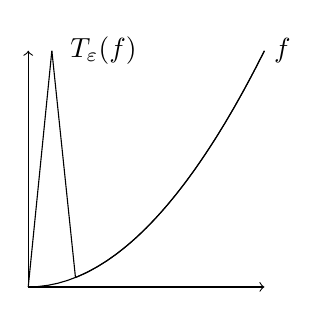
\begin{tikzpicture}[scale=3]
        \draw[->] (0, 0) -- (1, 0);
        \draw[->] (0, 0) -- (0, 1);

        \draw[domain=0:1, variable=\x] plot ({\x}, {\x^2}) node[right] {\( f \)};

        \draw (1/2, 1) node[left] {\( T_\varepsilon(f) \)};
        \draw[domain=0:0.1, variable=\x] plot ({\x}, {10 * \x});
        \draw[domain=0.1:0.2, variable=\x] plot ({\x}, {0.04 + (1 - 0.04) * (2 - 10 * \x)});
        \draw[domain=0.2:1, variable=\x] plot ({\x}, {\x^2});
      \end{tikzpicture}
    \end{Center}
  \end{figure}

  Define
  \begin{align*}
    T_\varepsilon(f)(x) \coloneqq \begin{cases}
      \frac x \delta_f, &0 \leq x < \delta_f \\
      f(\delta_f) + [1 - f(\delta_f)] (2 - \frac x {\delta_f}), &\delta_f \leq x < 2 \delta_f \\
      f(x), &x \geq 2 \delta_f,
    \end{cases}
  \end{align*}
  so that
  \begin{align*}
    \Norm{T_\varepsilon(f) - f}
    \geq
    T_\varepsilon(f) (\delta_f) - f(\delta_f)
    =
    1 - f(\delta_f)
    >
    1 - \varepsilon.
  \end{align*}

  Additionally, because \( \delta_{T_\varepsilon(f)} < \delta_f \), we have that \( f(\delta_{T_\varepsilon(f)}) < \varepsilon \) and
  \begin{align*}
    \Norm{T_\varepsilon(T_\varepsilon(f)) - f}
    \geq
    T_\varepsilon(T_\varepsilon(f)) (\delta_{T_\varepsilon(f)}) - f(\delta_{T_\varepsilon(f)})
    =
    1 - f(\delta_{T_\varepsilon(f)})
    >
    1 - \varepsilon.
  \end{align*}

  Thus, proceeding by induction, we see that for any \( m = 1, 2, \ldots \)
  \begin{align*}
    \Norm{T_\varepsilon^m(f) - f} > 1 - \varepsilon,
  \end{align*}
  where \( T_\varepsilon^m \) denotes repeated application of \( T_\varepsilon \).

  Consider the sequence
  \begin{align*}
    \{ T_\varepsilon^k(f) \}_{k=0}^\infty = \{ f, T_\varepsilon(f), T_\varepsilon(T_\varepsilon(f)), \ldots \}.
  \end{align*}

  We can easily see that the distance between any two elements of the sequence, say \( T_\varepsilon^k(f) \) and \( T_\varepsilon^{k+m}(f) \), is strictly greater that \( 1 - \varepsilon \), i.e.
  \begin{align*}
    \Norm{T_\varepsilon^k(f) - T_\varepsilon^{k+m}(f)}
    =
    \Norm{T_\varepsilon^k(f) - T_\varepsilon^m(T_\varepsilon^k(f))}
    >
    1 - \varepsilon.
  \end{align*}

  Hence \( B_1 \) cannot be covered by a finite \( (1-\varepsilon) \)-net and \( \alpha(B_1) \geq 1 - \varepsilon \). Since \( \varepsilon > 0 \) can be made arbitrarily small, this implies that \( \alpha(B_1) \geq 1 \) and, because we already have the reverse inequality, \( \alpha(B_1) = 1 \).

  In the set \( B_2 \), the maximum distance between two functions is \( \frac 1 2 \), thus \( \Diam(B_2) = \frac 1 2 \) and \( \alpha(B_2) \leq \frac 1 2 \). We can then define an operator similar to \( T_\varepsilon \) that creates \enquote{spikes} of height \( \frac 1 2 \) to prove the reverse inequality, obtaining
  \begin{align*}
    \alpha(B_2) = \frac 1 2.
  \end{align*}

  Finally, the set \( B_3 \) has diameter \( \frac 2 3 \) and hence \( \alpha(B_3) = \frac 2 3 \).

  The ball measure for \( B_1 \) satisfies the inequalities
  \begin{align*}
    \frac 1 2 \leq \beta(B_1) \leq 1.
  \end{align*}

  Additionally, \( B_1 \) is strictly contained in the ball centered in the constant function \( \frac 1 2 \) with radius \( \frac 1 2 \), which implies that \( \beta(B_1) \leq \frac 1 2 \), hence \( \beta(B_1) = \frac 1 2 \).

  For \( B_2 \) we have
  \begin{align*}
    \frac 1 4 \leq \beta(B_2) \leq \frac 1 2.
  \end{align*}

  Assume\LEM that for some \( \varepsilon > 0 \) the set \( B_2 \) can be covered by a finite set of balls with centers \( \{ f_1, \ldots, f_n \} \subsetneq C([0, 1]) \) and radius \( \frac 1 2 - \varepsilon \).

  Because of continuity, we can find a radius \( \delta > 0 \) such that for all \( f_k, k = 1, \ldots, n \) we have
  \begin{align*}
    x \in \left[\tfrac {1 - \delta} 2, \tfrac {1 + \delta} 2 \right] \implies \Abs{f_k(x) - f_k(\tfrac 1 2)} < \varepsilon.
  \end{align*}

  Consider the function
  \begin{align*}
    g(x) \coloneqq \begin{cases}
      0, &0 \leq x < \frac {1 - \delta} 2, \\
      \frac{2x + \delta - 1} {2\delta}, &\frac {1 - \delta} 2 \leq x \leq \frac {1 + \delta} 2, \\
      1, &\frac {1 + \delta} 2 < x \leq 1.
    \end{cases}
  \end{align*}

  \begin{figure}[ht]
    \begin{Center}
      \begin{tikzpicture}[scale=5]
        \draw[->] (0, 0) -- (1, 0);
        \draw[->] (0, 0) -- (0, 1);
        \draw[domain=0:4/10, thick, variable=\x] plot ({\x}, {0});
        \draw[domain=4/10:6/10, thick, variable=\x] plot ({\x}, {5 * \x - 2}) node[left] {\( g \)};
        \draw[domain=6/10:1, thick, variable=\x] plot ({\x}, {1});

        \draw[densely dotted] (0, 6/10) node[left] {\( f_k(\frac 1 2) - \varepsilon \)} -- (1, 6/10);
        \draw[densely dotted] (0, 8/10) node[left] {\( f_k(\frac 1 2) + \varepsilon \)} -- (1, 8/10);

        \draw[densely dotted] (4/10, 0) -- (4/10, 1);
        \draw (3/10, -1/10) node {\( \frac {1 - \delta} 2 \)};
        \draw[densely dotted] (1/2, 0) -- (1/2, 1);
        \draw (1/2, -1/10) node {\( \frac 1 2 \)};
        \draw[densely dotted] (6/10, 0) -- (6/10, 1);
        \draw (7/10, -1/10) node {\( \frac {1 + \delta} 2 \)};

        \draw[domain=-1/10:1, dash dot, variable=\x] plot ({\x}, {2/10 + 1 / (1 + e^(5/3*(1-2*\x)))}) node[right] {\( f_k \)};
      \end{tikzpicture}
    \end{Center}
  \end{figure}

  If \( f_k(\tfrac 1 2) \geq \frac 1 2 \), then \( f_k(\tfrac {1 - \delta} 2) > \tfrac 1 2 - \varepsilon \) and
  \begin{align*}
    \Norm{f_k - g} \geq f_k(\tfrac {1 - \delta} 2) - g(\tfrac {1 - \delta} 2) = f_k(\tfrac {1 - \delta} 2) > \tfrac 1 2 - \varepsilon.
  \end{align*}

  Analogously, if \( f_k(\tfrac 1 2) < \frac 1 2 \), then \( f_k(\tfrac {1 + \delta} 2) < \tfrac 1 2 + \varepsilon \) and
  \begin{align*}
    \Norm{g - f_k} \geq g(\tfrac {1 + \delta} 2) - f_k(\tfrac {1 + \delta} 2) = 1 - f_k(\tfrac {1 + \delta} 2) > \tfrac 1 2 - \varepsilon.
  \end{align*}

  Thus, for every \( k = 1, \ldots, n \) we have
  \begin{align*}
    \Norm{g - f_k} > \frac 1 2 - \varepsilon,
  \end{align*}
  i.e. \( g \) in not contained in a ball of radius \( \frac 1 2 - \varepsilon \) around any of the centers \( f_1, \ldots, f_n \).

  Hence \( \beta(B_2) \geq \frac 1 2 \), which implies \( \beta(B_2) = \frac 1 2 \). Because of the inclusion \( B_2 \subsetneq B_3 \subsetneq B_1 \), we have
  \begin{align*}
    \frac 1 2 = \beta(B_2) \leq \beta(B_3) \leq \beta(B_1) = \frac 1 2,
  \end{align*}
  hence \( \beta(B_3) = \frac 1 2 \).
\end{proof}

\begin{theorem}\label{thm:noncompact_kuratowski_lemma}[Kuratowski lemma]\cite[exercise 7.4]{Deimling1985}
  Let \( X \) be a Banach space and \( \{ A_n \}_n \) be a decreasing sequence of nonempty closed subsets such that \( \alpha(A_n) \to 0 \). Then \( A \coloneqq \bigcap_n A_n \) is nonempty and compact.
\end{theorem}
\begin{proof}
  The set \( A \) is compact because it is closed as the intersection of closed sets and \( \alpha(A) \leq \alpha(A_n) \to 0 \), hence \( \alpha(A) = 0 \).

  It remains to show that \( A \) is nonempty.
  Choose\AOC any sequence \( \{ x_n \}_n \) where \( x_n \in A_n \). Since any finite set is compact, we have that for any \( k \geq 1 \)
  \begin{align*}
    \alpha(\{ x_n \}_{n \geq 1})
    =
    \max\{ \alpha(\{ x_n \}_{n < k}), \alpha(\{ x_n \}_{n \geq k}) \}
    =
    \alpha(\{ x_n \}_{n \geq k})
    \leq
    \alpha(A_k) \to 0,
  \end{align*}
  hence the set \( \{ x_n \colon n \geq 1 \} \) is compact and thus sequentially compact. We can choose a convergent subsequence \( \{ x_{n_k} \}_k \) of \( \{ x_n \}_n \) whose limit lies in every \( A_n \) (since they are closed) and, consequently, in their intersection \( A \). So \( A \) is nonempty.
\end{proof}

  \subsection{Lipschitz continuity}\label{subsec:lipschitz_continuity}

\begin{definition}\label{def:lipschitz_continuity}
  Let \( f: X \to Y \) be a function between metric spaces.

  \begin{thmenum}
    \ilabel{def:lipschitz_continuity/holder} We say that \( f: X \to Y \) is \term{H\"older continuous} at \( x \in X \) with constant \( L \geq 0 \) and exponent \( \alpha > 0 \) if
    \begin{equation*}
      \rho_Y(f(x_1), f(x_2)) \leq L \rho_X(x_1, x_2)^\alpha \quad\forall x_1, x_2 \in X.
    \end{equation*}

    We refer to the smallest such constant, if any, as \enquote{the} H\"older constant.

    \ilabel{def:lipschitz_continuity/locally_holder} We say that \( f \) is \term{locally H\"older continuous} if every point has a neighborhood where \( f \) is H\"older continuous with the same exponent, but possibly with with a different constant.

    \ilabel{def:lipschitz_continuity/lipschitz} If \( \alpha = 1 \), we say that \( f \) is \term{Lipschitz continuous}.

    \ilabel{def:lipschitz_continuity/contraction} If \( X = Y \) and if \( f \) is Lipschitz with constant \( L < 1 \), we call \( f \) a \term{contraction mapping}.

    \ilabel{def:lipschitz_continuity/calm}\cite[53]{DontchevRockafellar2014} We say that \( f \) is \term{calm} at \( x \) if it satisfies the Lipschitz condition with one of the points fixed:
    \begin{equation*}
      \rho_Y(f(x), f(x')) \leq L \rho_X(x, x') \quad\forall x' \in X.
    \end{equation*}
  \end{thmenum}
\end{definition}

\begin{proposition}\label{thm:holder_map_is_uniformly_continuous}
  A H\"older map is uniformly continuous.
\end{proposition}
\begin{proof}
  Let \( f: X \to Y \) be a H\"older map with constant \( L \) and exponent \( \alpha \).

  Fix \( \varepsilon > 0 \). Then is enough to choose \( \delta < \sqrt[\alpha]{\frac \varepsilon L} \) so that
  \begin{equation*}
    \rho_X(x_1, x_2) < \delta \implies \rho_Y(f(x_1), f(x_2)) \leq L \rho_X(x_1, x_2)^\alpha < L \delta^\alpha < \varepsilon.
  \end{equation*}

  This implies uniform continuity.
\end{proof}

\begin{corollary}\label{thm:locally_holder_map_is_continuous}
  A locally H\"older map is continuous.
\end{corollary}

\begin{theorem}[Banach's fixed point theorem]\label{thm:banach_fixed_point_theorem}\mcite\cite[exer. 4.3.J]{Engelking1989}
  A contraction \hyperref[def:lipschitz_continuity/contraction]{mapping} in a \hyperref[def:complete_metric_space]{complete metric space} has a unique fixed \hyperref[def:fixed_point]{point}.
\end{theorem}
\begin{proof}
  Let \( f: X \to X \) be a contraction mapping. Fix any point \( x_0 \in X \) and inductively define the sequence
  \begin{equation*}
    x_{k+1} \coloneqq f(x_k), k = 1, 2, \ldots.
  \end{equation*}

  Fix \( \varepsilon > 0 \). Since \( L < 1 \), there exists an index \( k_0 > \log_L(\varepsilon) \) such that for positive integers \( m \) and \( k > k_0 \),
  \begin{balign*}
    \rho(x_k, x_{k+m})
     & =
    \rho(f^k(x_0), f^{k+m}(x_0))
    \leq \\ &\leq
    L^k \rho(x_0, x_m)
    <    \\ &<
    \varepsilon \rho(x_0, x_m).
  \end{balign*}

  Note that
  \begin{balign*}
    \rho(x_0, x_m)
     & \leq
    \sum_{i=1}^m \rho(x_{i-1}, x_i)
    \leq    \\ &\leq
    \rho(x_0, x_1) \sum_{i=1}^m L^{i-1}
    =       \\ &=
    \rho(x_0, x_1) \frac {1 - L^m} {1 - L}
    \leq    \\ &\leq
    \rho(x_0, x_1) \frac 1 {1 - L}.
  \end{balign*}

  Thus
  \begin{equation*}
    \rho(x_k, x_{k+m}) < \frac {\varepsilon \rho(x_0, x_1)} {1 - L}.
  \end{equation*}

  The constant on the right is linear in \( \varepsilon \) and does not depend on \( k \) or \( m \), hence \( \{ x_k \}_{k=0}^\infty \) is a fundamental sequence. Since \( X \) is complete, the sequence has a limit \( x \).

  Because of the continuity of \( f \) (see \fullref{thm:holder_map_is_uniformly_continuous}),
  \begin{equation*}
    f(x) = f(\lim_{k \to \infty} x_k) = \lim_{k \to \infty} f(x_k) = \lim_{k \to \infty} x_{k+1} = x.
  \end{equation*}
\end{proof}

  \subsection{Function oscillation}\label{subsec:function_oscillation}

\begin{definition}\label{def:function_oscillation}
  Let \( \CX \) be a nonempty set and \( (\CY, \rho_{\CY}) \) be a metric space. We define the \Def{oscillation} of a function on a set as
  \begin{BreakableAlign*}
     &\omega: \Func(\CX, \CY) \times \Pow(\CX) \to [0, \infty] \\
     &\omega(f, A) \coloneqq \sup \Big\{ \rho_{\CY}(f(x), f(y)) \colon (x, y) \in A \Big\}.
  \end{BreakableAlign*}

  In particular, if \( \CX \) is itself a metric space, we define its \Def{modulus of continuity} \( \omega(f, \delta) \) as the oscillation of \( f \) on the ball \( B(0, \delta) \).
\end{definition}

\begin{proposition}\label{thm:modulus_of_continuity_properties}
  The \hyperref[def:modulus_of_continuity]{modulus of continuity} has the following basic properties:
  \begin{PropEnum}
    \ILabel{thm:modulus_of_continuity_properties/continuity_condition} \( f \) is globally \hyperref[def:uniform_continuity]{uniformly continuous} if and only if for every \( \varepsilon > 0 \) there exists \( \delta > 0 \) such that \( \omega(f, \delta) \).

    \ILabel{thm:modulus_of_continuity_properties/monotone} \( \omega(f, \delta) \) is monotone in \( \delta \).

    \ILabel{thm:modulus_of_continuity_properties/cauchy_inequality}\MarginCite[28]{Николов2020}For all \( \lambda, \delta > 0 \), we have the following analog of \fullref{thm:cauchy_bunyakovsky_schwarz_inequality}
    \begin{equation}\label{thm:modulus_of_continuity_properties/cauchy_inequality/inequality}
      \omega(f, \lambda \delta) \leq \omega(f, \lambda^2) + \omega(f, \delta^2).
    \end{equation}

    \ILabel{thm:modulus_of_continuity_properties/single_inequality}\MarginCite[28]{Николов2020}For all \( \lambda, \delta > 0 \),
    \begin{equation}\label{thm:modulus_of_continuity_properties/single_inequality/inequality}
      \omega(f, \lambda \delta) \leq (\lambda + 1) \omega(f, \delta).
    \end{equation}
  \end{PropEnum}
\end{proposition}
\begin{proof}
  \SubProofOf{thm:modulus_of_continuity_properties/continuity_condition} Follows directly from \fullref{def:uniform_continuity}.

  \SubProofOf{thm:modulus_of_continuity_properties/monotone} A supremum on a larger set is larger.

  \SubProofOf{thm:modulus_of_continuity_properties/cauchy_inequality} If \( \lambda \leq \delta \), clearly \( \lambda \delta \leq \delta^2 \). Otherwise, \( \lambda \delta < \lambda^2 \).

  Combining the two inequalities with \fullref{thm:modulus_of_continuity_properties/monotone}, we obtain \fullref{thm:modulus_of_continuity_properties/cauchy_inequality/inequality}.

  \SubProofOf{thm:modulus_of_continuity_properties/single_inequality} Note that
  \begin{equation*}
    \rho_{\CX}(x, y) < \delta \Timplies \rho_{\CY}(f(x), f(y)) < \omega(f, \delta).
  \end{equation*}

  We can multiply this by \( \lambda \) to obtain
  \begin{equation*}
    \lambda \rho_{\CX}(x, y) < \lambda \delta \Timplies \lambda \rho_{\CY}(f(x), f(y)) < \lambda \omega(f, \delta).
  \end{equation*}

  If \( \lambda \geq 1 \), then \( \rho_{\CX}(x, y) \leq \lambda \rho_{\CX}(x, y) \) and \( \rho_{\CY}(f(x), f(y)) \leq \lambda \rho_{\CY}(f(x), f(y)) \) and hence
  \begin{equation*}
    \omega(f, \lambda \delta) \leq \lambda \omega(f, \delta).
  \end{equation*}

  Otherwise, \( \lambda < 1 \) and clearly \( \lambda \delta < \delta \), which by \fullref{thm:modulus_of_continuity_properties/monotone} implies
  \begin{equation*}
    \omega(f, \lambda \delta) \leq \omega(f, \delta).
  \end{equation*}

  Combining the two cases, we obtain
  \begin{equation*}
    \omega(f, \lambda \delta) \leq \lambda \omega(f, \delta) + \omega(f, \delta),
  \end{equation*}
  which we wanted to prove.
\end{proof}


  \section{Geometry}\label{sec:geometry}

Humans possess a strong intuition for visual information like drawings or diagrams. A drawing on a paper is only a medium for communicating ideas and data. \Fullref{fig:sec:geometry/figures} contains some highlighted curves that our mind maps to abstract geometric figures, without considering the size limitations of the page, the precision of the drawings or the thickness of the lines.

\begin{figure}[!ht]
  \centering
  \includegraphics{output/sec__geometry__figures.pdf}
  \caption{A \hyperref[def:triangle]{triangle}, a \hyperref[def:circle]{circle} and a \hyperref[def:affine_line]{line} in the \hyperref[def:euclidean_space]{Euclidean plane}.}\label{fig:sec:geometry/figures}
\end{figure}

Our goal is to introduce formalisms for these mental visualizations. An axiomatic approach for a theory of figures in the place and space was developed by Euclid in the third century BC and can be found in \cite{Fitzpatrick2008}. A few millennia later, several mathematicians proposed systems of axioms that fit the requirements of \hyperref[sec:mathematical_logic]{modern logical systems}. Tarski's system can be found in \cite{Tarski1959}. This is known today as \term{synthetic Euclidean geometry} and is mostly of theoretical interest.

An important distinction between ancient and modern geometry is the introduction of coordinates in the 17th century. Descartes' idea of coordinates connects problems of algebra and geometry in such a way that most of today's mathematics seamlessly switches between algebraic and geometric interpretations of the same problem. The study of classical Greek geometry in terms of coordinates is known as \term{analytic geometry}.

A modern interpretation if the ideas behind analytic geometry leads to \hyperref[def:affine_spaces]{affine spaces}, which we will discuss in \fullref{subsec:affine_spaces} and \fullref{subsec:convex_sets}, to Euclidean spaces discussed in \fullref{subsec:euclidean_spaces} and to the Euclidean plane discussed in \fullref{subsec:euclidean_plane}, \fullref{subsec:triangles} and \fullref{subsec:quadratic_plane_curves}. As part of our discussion of the \hyperref[def:euclidean_plane]{Euclidean plane}, we will briefly introduce modern concepts related to differential geometry in \fullref{subsec:parametric_curves} and algebraic geometry in \fullref{subsec:quadratic_plane_curves}.

  \section{Geometry}\label{sec:geometry}

\begin{remark}\label{def:coordinates_in_geometry}
  Geometry is the multi-millennium evolution of attempts to measure parts of the earth. Ironically, it may be the main historical justification for the gradual axiomatization of mathematics. Completely abstract results about shapes date at least as early as in Ancient Greece. The important distinction between ancient geometry and modern geometry is the introduction of coordinates in the 17th century.

  An axiomatic approach for a theory of plane and solid figures was developed by Euclid in the third century BC. Later, Hilbert, Tarski and others independently proposed axioms that fit the requirements of modern logic systems. This is known today as \Def{synthetic Euclidean geometry} and is mostly of theoretical interest because modern tools are easier to work with.

  Descartes' idea of coordinates connects problems of algebra and geometry in such a way that most of today's mathematics seamlessly switches between algebraic and geometric interpretations of the same problem. The study of classical Greek geometry in terms of coordinates is known as \Def{analytic geometry}.
\end{remark}

\subsection{Affine coordinate systems}\label{subsec:affine_coordinate_system}

\begin{remark}\label{rem:affine_coordinate_system_concept}
  Most humans possess a strong intuition for visual information like drawings or diagrams. A paper or a painting is only a medium for communicating information and emotions. \Fullref{def:euclidean_plane/figures} contains some highlighted curves that our mind maps to abstract geometric figures, without considering the size limitations of the page, the precision of the drawings or the thickness of the lines.

  \begin{figure}[b]
    \centering
    \begin{mplibcode}
      u := 1cm;

      beginfig(1);
      draw (0, -1) * u -- (3, 0) * u;
      draw (-1, 2) * u -- (3, 1) * u -- (1, 3) * u -- cycle;
      draw fullcircle scaled 1.5u shifted ((0, 0.5) * u);
      endfig;
    \end{mplibcode}
    \Caption{def:euclidean_plane/figures}{A triangle, a circle and a line in the Euclidean plane.}
  \end{figure}

  Our goal is to map these visualizations to the concept of vector spaces. Formalisms at the level of formal \hyperref[def:first_order_logic_alphabet]{logic} will not be stated because we only want to sketch some high-level concepts. We only give definitions that are strictly necessary, plane geometry itself is described in \fullref{subsec:analytic_geometry_in_the_plane}. We will proceed as follows:

  \begin{itemize}
    \item Define an affine plane in \fullref{def:affine_plane} with auxiliary definitions.
    \item Describe the Euclidean plane \( A_2 \) in \fullref{def:euclidean_plane} as a very special affine plane.
    \item Give additional definitions for the Euclidean plane in \fullref{def:euclidean_plane_auxiliary_definitions}.
    \item Define the set \( F_2 \) of free vectors over \( A_2 \) in \fullref{def:euclidean_plane_free_vector}.
    \item Show that \( F_2 \) is a two-dimensional vector space over \( \BR \) in \fullref{thm:euclidean_plane_factorization}.
    \item Define coordinate systems that give explicit isomorphisms between \( A_2 \), \( F_2 \) and \( \BR^2 \) in \fullref{def:euclidean_plane_coordinate_system}.
    \item Generalize these notions in \fullref{rem:coordinate_systems}
  \end{itemize}
\end{remark}

\begin{definition}\label{def:affine_plane}\MarginCite[1]{Hartshorne1967}
  An \Def{affine plane} consists of
  \begin{itemize}
    \item a set \( X \), whose elements are called \Def{points},
    \item a family of subsets of \( X \), whose members are called \Def{lines}
  \end{itemize}
  with the additional relations
  \begin{itemize}
    \item a \Def{parallel} relation \( l \parallel g \) for lines that holds if either \( l = g \) or if they have no points in common,
    \item a \Def{collinearity} relation for a set \( B \) of points that holds if \( B \) is a subset of some line,
  \end{itemize}
  such that
  \begin{DefEnum}
    \IAxiom{def:affine_plane/A1}{A1} Given two distinct points, there exists only one line that contains both.
    \IAxiom{def:affine_plane/A2}{A2} Given a line \( l \) and a point \( P \not\in l \), there exists exactly one line \( g \parallel l \) that contains \( P \).
    \IAxiom{def:affine_plane/A3}{A3} There exist three non-collinear points.
  \end{DefEnum}
\end{definition}

\begin{definition}\label{def:euclidean_plane}
  The \Def{Euclidean plane} \( A_2 \) is a formalization of a straight infinite surface. An axiomatic definition can be found in \cite{nLab:euclidean_geometry}. We will use that
  \begin{itemize}
    \item The Euclidean plane \( A_2 \) is an \hyperref[def:affine_plane]{affine plane}
    \item \( A_2 \) is a \hyperref[def:complete_metric_space]{complete metric space} with distance \( \Dist \).
    \item There is a \Def{betweenness} relation for points that says if the point \( R \) is \Def{between} \( P \) and \( Q \).
  \end{itemize}

  \begin{figure}
    \centering
    \begin{mplibcode}
      input metapost/plotting;

      u := 1.5cm;

      beginfig(1);
      path l, g, h, P, Q, R;
      l = (0, -1) * u -- (3, 0) * u;
      draw l;
      label.top("$l$", midpoint of l);

      g = (0, -2) * u -- (3, -1) * u;
      draw g;
      label.bot("$g$", midpoint of g);

      h = (0, 0) * u -- (3, -2) * u;
      draw h;
      label.urt("$h$", midpoint of h);

      P = dot shifted point 0.2 of h;
      fill P;
      label.llft("$P$", midpoint of P);

      Q = dot shifted point 0.8 of h;
      fill Q;
      label.llft("$Q$", midpoint of Q);

      R = dot shifted point 0.4 of h;
      fill R;
      label.llft("$R$", midpoint of R);
      endfig;
    \end{mplibcode}
    \Caption{def:affine_plane/figure}{Three lines and three points in the Euclidean plane. The lines \( l \) and \( g \) are collinear, while the point \( R \) is between \( P \) and \( Q \)}
  \end{figure}
\end{definition}

\begin{definition}\label{def:euclidean_plane_auxiliary_definitions}
  We will also need the following definitions:
  \begin{DefEnum}
    \ILabel{def:affine_plane/half_plane} Every line \( l \) gives rise to two (closed) \Def{half-planes} \( H^+ \) and \( H^- \) as follows:
    \begin{itemize}
      \item \( H^+ \cap H^- = l \)
      \item \( H^+ \cup H^- = A_2 \)
      \item If \( P \in H^+ \setminus l \) and \( Q \in H^- \setminus l \), then there is a point \( R \in l \) between \( P \) and \( Q \)
    \end{itemize}

    Note that the superscripts \( + \) and \( - \) are only for distinguishing between the two half-planes and are not assigned based on some property of the half-planes. See \fullref{def:half_space} for a definition of a half-plane that actually has a concept of signs.

    \begin{figure}
      \centering
      \begin{mplibcode}
        input metapost/plotting;

        u := 1cm;

        beginfig(1);
        input hatching;

        path l, Hp, Hm;
        l = (0, -1) * u -- (3, 0) * u;
        draw l;

        Hp = l -- (3, 0.5) * u -- (0, 0.5) * u -- cycle;
        hatchfill Hp withcolor (45, 1mm, -.5bp);
        label.ulft("$H^+$", startpoint of l);

        Hm = l -- (3, -1.5) * u -- (0, -1.5) * u -- cycle;
        hatchfill Hm withcolor (135, 1mm, -.5bp);
        label.lrt("$H^-$", endpoint of l);
        endfig;
      \end{mplibcode}

      \Caption{def:affine_plane/bound_vector/half_plane}{Differently hatched half-planes in the Euclidean plane.}
    \end{figure}

    \ILabel{def:affine_plane/ray} Every line \( l \) and every point \( R \) give rise to two (closed) \Def{rays} \( l^+ \) and \( l^- \) as follows:
    \begin{itemize}
      \item \( l^+ \cap l^- = \{ R \} \) are disjoint
      \item \( l^+ \cup l^- = l \)
      \item If \( P \in l^+ \setminus \{ R \} \) and \( Q \in l^- \setminus \{ R \} \), then \( R \) is between \( P \) and \( Q \)
    \end{itemize}

    The rays \( l^+ \) and \( l^- \) are called \Def{opposite} of each other.

    We say that \( R \) is the \Def{vertex} of \( l^+ \) and \( l^- \).

    See \fullref{def:geometric_ray} for a definition of a ray that actually has a concept of signs.

    \begin{figure}
      \centering
      \begin{mplibcode}
        input metapost/plotting;

        u := 1cm;

        beginfig(1);
        path l, R;

        l = (0, -1) * u -- (3, 0) * u;
        drawdblarrow l;
        label.lft("$l^-$", startpoint of l);
        label.rt("$l^+$", endpoint of l);

        R = dot shifted midpoint of l;
        fill R;
        label.bot("$R$", midpoint of R);
        endfig;
      \end{mplibcode}

      \Caption{def:affine_plane/day/figure}{Opposite rays in the Euclidean plane.}
    \end{figure}

    \ILabel{def:affine_plane/rays_unidirectional} Two rays are said to be \Def{unidirectional} if there exists a line distinct from the lines containing the rays, such that both rays are contained in the same half-plane with respect to the line.

    \ILabel{def:affine_plane/bound_vector} An ordered pair \( \Vect{PQ} \) of points is called a \Def{bound vector}. The point \( P \) is called the \Def{beginning} of \( \Vect{PQ} \) and \( Q \) is called the \Def{end} of \( \Vect{PQ} \).

    \begin{figure}
      \centering
      \begin{mplibcode}
        input metapost/plotting;

        u := 0.75cm;

        beginfig(1);
        path P, Q, R, PQ, PR;

        PQ = (0, -1) * u -- (3, 0) * u;
        drawarrow PQ;
        label.bot("$\Vect{PQ}$", midpoint of PQ);

        P = dot shifted startpoint of PQ;
        fill P;
        label.bot("$P$", midpoint of P);

        Q = dot shifted endpoint of PQ;
        label.bot("$Q$", midpoint of Q);

        PR = (0, -1) * u -- (-2, 0.5) * u;
        drawarrow PR;
        label.llft("$\Vect{PR}$", midpoint of PR);

        R = dot shifted endpoint of PR;
        label.llft("$R$", midpoint of R);
        endfig;
      \end{mplibcode}

      \Caption{def:affine_plane/bound_vector/figure}{Bound vectors in the Euclidean plane can be regarded as oriented line segment.}
    \end{figure}
  \end{DefEnum}
\end{definition}

\begin{definition}\label{def:euclidean_plane_free_vector}
  We say that the bound vectors \( \Vect{P_1 Q_1} \) and \( \Vect{P_2 Q_2} \) in \( A_2 \) are \Def{congruent} if \( \Dist(P_1, Q_1) = \Dist(P_2, Q_2) \) and if the rays \( r_i, i = 1, 2 \) beginning at \( P_i \) and containing \( Q_i \), are unidirectional.

  We define \Def{free vectors} as \hyperref[thm:equivalence_partition]{equivalence classes} of bound vectors by this congruence relation. We denote the corresponding equivalence partition by \( F_2 \).
\end{definition}

\begin{theorem}\label{thm:euclidean_plane_factorization}
  The set \( F_2 \) of free vectors over \( A_2 \) is a two-dimensional \hyperref[def:vector_space]{vector space} over \( \BR \) with the following operations:
  \begin{ThmEnum}
    \ILabel{thm:euclidean_plane_factorization/sum} We define the \Def{sum} of the cosets \( [\Vect{PQ}] \) and \( [\Vect{QR}] \) as the coset \( [\Vect{PR}] \).

    \ILabel{thm:euclidean_plane_factorization/scalar_product} We define the \Def{scalar multiplication} of \( \lambda \in \BR \) with the coset \( [\Vect{PQ}] \) to be the coset \( [\Vect{PR}] \), where \( \Vect{PR} \) is the unique vector that is unidirectional with \( \Vect{PQ} \) and \( \Dist(P, R) = \lambda \Dist(P, Q) \).
  \end{ThmEnum}
\end{theorem}
\begin{proof}
  Proving the well-definedness of the operations and verifying that \( F_2 \) is a two-dimensional vector space requires a lot of work and the proof is skipped.
\end{proof}

\begin{definition}\label{def:euclidean_plane_coordinate_system}
  Just because \fullref{thm:euclidean_plane_factorization} states that the set \( F_2 \) of free vectors is a vector space does not mean that we can work with it as with \( \BR^2 \). \Fullref{thm:finite_dimensional_spaces_are_isomorphic} says that \( F_2 \) is isomorphic to \( \BR^2 \), however the proof requires the axiom of \hyperref[def:set_zfc/A9]{choice}. The concrete way to select a basis in \( F_2 \) is through coordinate systems.

  Somewhat confusingly, we define coordinate systems over \( A_2 \) rather than over \( F_2 \), but this will soon be justified.

  A \Def{coordinate system} \( Oxy \) in \( A_2 \) is a choice of
  \begin{DefEnum}
    \ILabel{def:euclidean_plane_coordinate_system/origin} A point \( O \in A_2 \), called the \Def{origin} of the coordinate system.
    \ILabel{def:euclidean_plane_coordinate_system/basis} An \hyperref[def:poset]{ordered} \hyperref[def:left_module_hamel_basis]{basis} \( (x, y) \) of \( F_2 \), called the \Def{basis} of \( Oxy \).
  \end{DefEnum}

  What we achieve through the choice of \( O \) is that, for each point \( P \in A_2 \), we select the bound vector \( \Vect{OP} \in V_2 \), called the \Def{radius vector} of \( P \). This injects \( A_2 \) into \( V_2 \), however if we take the free vector \( [\Vect{OP}] \), we instead obtain a bijection between \( A_2 \) and \( F_2 \).

  Now that we have a correspondence between \( A_2 \) and \( F_2 \), coordinates for the point \( P \) are defined simply as the \hyperref[def:left_module_basis_projection]{coordinates} of \( [\Vect{OP}] \) with respect to the basis \( (x, y) \).

  Thus the pair \( (A_2, Oxy) \) has an explicit isomorphism with \( \BR^2 \).

  The \Def{coordinate axis} of \( x \) is the unique \hyperref[def:affine_plane/ray]{ray} starting at \( O \) and containing the end of \( x \). It is called the \Def{abscissa}. The coordinate axis of \( y \) is called the \Def{ordinate}.
\end{definition}

\begin{remark}\label{rem:coordinate_systems}
  We sketched how to embed mental images of planes into \( \BR^2 \), however in mathematics we are often interested in the opposite: given a set of points in \( \BR^2 \), visualize them on a screen or paper and then absorb the the resulting image in our brain.

  This is one of the most powerful constructions in mathematics, yet it is so intuitive that it is not really given a lot of attention, at least until generalizations are required. Given any vector space \( V \) in the sense of \fullref{def:vector_space}, we want a way to assign a pair of numbers to each vector in \( V \). This is only possible if \( \dim V = 2 \), however we can generalize this to tuples of coordinates via bases - see \fullref{def:left_module_hamel_basis}. This well for finitely dimensional vector spaces, however we need to generalize these notion for infinitely dimensional vector spaces and general modules over \hyperref[def:left_module]{rings}. This allows us to generalize coordinates further to manifolds - see \fullref{def:topological_manifold}.

  See \fullref{subsec:vector_space_geometry} for immediate generalizations of the concepts introduced here.
\end{remark}

  \subsection{Vector space geometry}\label{subsec:vector_space_geometry}

We will denote by \( \BbbK \) either the field of \hyperref[def:real_numbers]{real numbers} or the \hyperref[def:real_numbers]{complex numbers}. We will mostly work over the real numbers, but some important definitions and theorems hold more generally. Unless otherwise noted, \( X \) is a vector space over \( \BbbK \).

\begin{remark}\label{rem:real_field_extensions}
  When speaking about vector spaces, we usually restrict ourselves to vector spaces over \( \BbbR \) or, at most, \( \BbbC \). This restriction may seem arbitrary, however important concepts like \hyperref[def:geometric_ray]{rays} or \hyperref[def:convex_hull]{convexity} requires the field to be an extension of \( \BbbR \), and it just so happens that, by \fullref{thm:fundamental_theorem_of_algebra} and \fullref{thm:no_finite_extensions_of_closed_fields}, the only nontrivial finite \hyperref[def:field/submodel]{field extension} of \( \BbbR \) is \( \BbbC \). It is technically possible to work with infinite field extensions, however in practice vector spaces over \( \BbbC \) are esoteric enough.

  Considering only \( \BbbR \) and \( \BbbC \) leads to certain concepts being defined for complex vector spaces and then real vector spaces become a special case. This is formalized via \hyperref[def:complexification]{complexification}. For example, inner products are defined in \fullref{def:inner_product_space} differently for real and complex vector spaces, however we can transition between them due to \fullref{thm:complexification_universal_property} and \fullref{thm:complexification_of_symmetric_bilinear_form}.
\end{remark}

\begin{definition}\label{def:geometric_shape}
  A \term{geometric shape} is an informal notion that refers to certain special subsets of a vector space, usually defined in a coordinate-independent manner. Shapes in two-dimensional spaces are called \term{figures} and shapes in three dimensions are called \term{surfaces}.

  When two geometric shapes intersect, we say that they are \term{incident}. This relates to \hyperref[def:hypergraph/incidence]{(hyper)graph incidence} via \hyperref[def:quiver_geometric_realization]{geometric realizations}.

  We are interested in the following:
  \begin{thmenum}
    \thmitem{def:geometric_shape/parametric} Parametric shape, defined in \fullref{def:parametric_shape}, are a topological construction.
    \thmitem{def:geometric_shape/algebraic} Affine varieties, defined in \fullref{def:affine_algebraic_set}, are an algebraic construction.
    \thmitem{def:geometric_shape/geometric} Manifolds, defined in \fullref{def:topological_manifold}, are a geometric construction.
  \end{thmenum}

  All the above have a concept of dimension. Shapes of dimension \( 1 \) are called \term{curves}.
\end{definition}

\begin{definition}\label{def:point}
  A \term{point} is a simple \hyperref[def:geometric_shape]{geometric shape} comprising a singleton subset of a topological space. We use the convention \fullref{rem:singleton_sets} and, unless the distinction is important, we do not distinguish between singleton sets and their only element --- see \fullref{def:simplex/point} for an example.

  Within vector spaces points are also called vectors, which is justified by \fullref{def:euclidean_plane_coordinate_system}.

  Scalar multiplication, when applied to points, is also called \term{dilation}.
\end{definition}

\begin{definition}\label{def:affine_hull}\mimprovised
  We say that the \hyperref[rem:linear_combinations]{linear combination}
  \begin{equation*}
    t_1 x_1 + \ldots + t_n x_n
  \end{equation*}
  with real coefficients is an \term{affine combination} if
  \begin{equation*}
    t_1 + \cdots + t_n = 1.
  \end{equation*}

  The \term{affine hull} of the set \( S \) is the set of all affine combinations of members of \( S \). This can be expressed succinctly by saying that, for any real number \( \lambda \) and any vectors \( x \) and \( y \), the hull must contain
  \begin{equation}\label{eq:def:affine_hull/combination}
    \lambda x + (1 - \lambda) y.
  \end{equation}

  The affine hull is a \hyperref[def:closure_operator]{closure operator}.

  Geometrically, the affine hull of \( S \) is the smallest translated vector subspace of \( X \). Unlike the linear span, the affine hull does not necessarily contain the zero vector because it is not itself a vector subspace, but a translation of one. See \cref{fig:def:convex_hull}.
\end{definition}
\begin{defproof}
  We will show that the affine hull operator \( A: \pow(X) \to \pow(X) \) is a closure operator.

  \SubProofOf[def:inflationary_function]{inflation} Obviously \( S \subseteq A(S) \).

  \SubProofOf[def:magma/idempotent]{idempotence} Consider the affine combination \( \lambda x + (1 - \lambda) y \) of vectors from \( A(S) \). Suppose that \( x = t_x u_x + (1 - t_x) v_x \) and \( y = t_y u_y + (1 - t_y) v_y \), where \( u_x \), \( u_y \), \( v_x \) and \( v_y \) are vectors from \( S \).

  Then
  \begin{equation*}
    \lambda x + (1 - \lambda) y
    =
    \lambda t_x u_x + \lambda (1 - t_x) v_x + (1 - \lambda) t_y u_y + (1 - \lambda) (1 - t_y) v_y.
  \end{equation*}

  This is an affine combination of members of \( S \). Therefore, \( A(A(S)) = A(S) \).

  \SubProofOf[eq:def:partially_ordered_set/homomorphism/nonstrict]{monotonicity} If \( S_1 \subseteq S_2 \), then \( A(S_2) \) contains the affine combinations of the members of \( S_1 \) in addition to others. Hence, \( A(S_1) \subseteq A(S_2) \).
\end{defproof}

\begin{definition}\label{def:affine_operator}
  We say that the function \( f: X \to Y \) between vector spaces over \( \BbbK \) is an \term{affine operator} if any of the following equivalent conditions hold:
  \begin{thmenum}
    \thmitem{def:affine_operator/translation} The map \( T(x) \coloneqq f(x) - f(0) \) is a linear operator.
    \thmitem{def:affine_operator/combination} \( f \) preserves \hyperref[def:affine_hull]{affine combinations}. That is, for any real number \( \lambda \),
    \begin{equation}\label{eq:def:affine_operator/combination}
      f\parens[\Big]{ \lambda x + (1 - \lambda) y } = \lambda f(x) + (1 - \lambda) f(y).
    \end{equation}
  \end{thmenum}
\end{definition}
\begin{defproof}
  \ImplicationSubProof{def:affine_operator/translation}{def:affine_operator/combination} Suppose that \( T \) is linear. Then for an arbitrary real number \( \lambda \),
  \begin{balign*}
    f(\lambda x + (1 - \lambda) y)
    &=
    T(\lambda x + (1 - \lambda) y) + f(0)
    = \\ &=
    \lambda T(x) + (1 - \lambda) T(y) + f(0)
    = \\ &=
    \lambda \parens[\Big]{ f(x) - f(0) } + (1 - \lambda) \parens[\Big]{ f(y) - f(0) } + f(0)
    = \\ &=
    \lambda f(x) + (1 - \lambda) f(y).
  \end{balign*}

  We can cancel \( f(0) \) to obtain \eqref{eq:def:affine_operator/combination}.

  \ImplicationSubProof{def:affine_operator/combination}{def:affine_operator/translation} Suppose that \eqref{eq:def:affine_operator/combination} holds. Then
  \begin{balign*}
    T(x + y)
    &=
    f(x + y) - f(0)
    = \\ &=
    f(1 \cdot x - 1 \cdot 0 + 1 \cdot y - 1 \cdot 0 + 1 \cdot 0) - f(0)
    = \\ &=
    \parens[\Big]{ f(x) - f(0) } + \parens[\Big]{ f(y) - f(0) } + f(0) - f(0)
    = \\ &=
    T(x) + T(y).
  \end{balign*}

  Also,
  \begin{equation*}
    T(\lambda x)
    =
    f(\lambda x + (1 - \lambda) 0) - f(0)
    =
    \lambda f(x) - \lambda f(0)
    =
    \lambda T(x).
  \end{equation*}

  This shows that \( T \) is a linear operator.
\end{defproof}

\begin{proposition}\label{thm:isometry_iff_affine_orthogonal_operator}\mcite[thm. 7.1]{Treil2017}
  The endofunction \( f: X \to X \) over the real inner product space \( X \) is an \hyperref[def:isometry]{isometry} if and only if it is an \hyperref[def:affine_operator]{affine operator} whose linear part \( T(x) \coloneqq f(x) - f(0) \) is \hyperref[def:unitary_operator]{orthogonal}.
\end{proposition}
\begin{proof}
  \SufficiencySubProof Suppose that \( f \) is an isometry.

  First note that
  \begin{equation*}
    \inprod { f(x) } { f(y) } = \inprod x y.
  \end{equation*}

  Indeed, we have
  \begin{equation*}
    \norm{ f(x) - f(y) } = \norm{ f(x) } + \norm{ f(y) } - 2 \inprod { f(x) } { f(y) }
  \end{equation*}
  and
  \begin{equation*}
    \norm{ x - y } = \norm x + \norm y - 2 \inprod x y.
  \end{equation*}

  Therefore,
  \begin{equation*}
    \inprod { f(x) } { f(y) }
    =
    \frac{ \norm{ f(x) - f(y) } - \norm{ f(x) } - \norm{ f(y) } } 2
    =
    \frac{ \norm{ x - y } - \norm{ x } - \norm{ y } } 2
    =
    \inprod x y.
  \end{equation*}

  Now we can show additivity of \( T \):
  \begin{balign*}
    &\phantom{{}={}}
    \norm{ T(x + y) - T(x) - T(y) }^2
    = \\ &=
    \norm{ f(x + y) - f(0) - f(x) + f(0) - f(y) + f(0) }^2
    = \\ &=
    \norm{ \parens{ f(x + y) - f(x) } - \parens{ f(y) - f(0) } }^2
    = \\ &=
    \norm{ f(x + y) - f(x) }^2 + \norm{ f(y) - f(0) }^2 - 2 \inprod{ f(x + y) - f(x) } { f(y) - f(0) }
    = \\ &=
    \norm{ x + y - x }^2 + \norm{y}^2 - 2 \inprod{x + y} y + 2 \inprod x y - 2 \inprod {x + y} 0 + 2 \inprod x 0
    = \\ &=
    2 \norm{y}^2 - 2 \inprod x y - 2 \norm{y}^2 + 2 \inprod x y.
  \end{balign*}

  The norm is zero, hence \( T(x + y) = T(x) + T(y) \).

  Similarly,
  \begin{balign*}
    &\phantom{{}={}}
    \norm{ T(\lambda x) - \lambda T(x) }^2
    = \\ &=
    \norm{ f(\lambda x) - f(0) - \lambda f(x) + \lambda f(0) }^2
    = \\ &=
    \norm{ f(\lambda x) - f(0) }^2 + \norm{ \lambda f(x) - \lambda f(0) }^2 - 2 \inprod{ f(\lambda x) - f(0) } { \lambda f(x) - \lambda f(0) }
    = \\ &=
    \norm{\lambda x}^2 + \lambda^2 \norm{x}^2 - 2 \lambda \inprod{ f(\lambda x) - f(0) } { f(x) - f(0) }
    = \\ &=
    2 \lambda^2 \norm{x}^2 - 2 \lambda^2 \inprod x x.
  \end{balign*}

  This norm is also zero, hence \( T(\lambda x) = \lambda T(x) \).

  Finally, we must show that \( T \) is a unitary operator:
  \begin{balign*}
    \inprod{ T(x) }{ T(y) }
    &=
    \inprod{ f(x) - f(0) }{ f(y) - f(0) }
    = \\ &=
    \inprod{ f(x) }{ f(y) } - \inprod{ f(x) }{ f(0) } - \inprod{ f(0) }{ f(y) } + \inprod{ f(0) }{ f(0) }
    = \\ &=
    \inprod x y.
  \end{balign*}

  \NecessitySubProof Suppose that \( f(x) = Tx + f_0 \) for some unitary operator \( T \) and some vector \( f_0 \). Then
  \begin{balign*}
    \norm{ f(x) - f(y) }^2
    &=
    \norm{ Tx - f_0 - Ty + f_0 }^2
    = \\ &=
    \norm{ T(x - y) }^2
    = \\ &=
    \inprod{ T(x - y) }{ T(x - y) }
    = \\ &=
    \inprod{ x - y }{ T^{-1} T(x - y) }
    = \\ &=
    \norm{ x - y }^2.
  \end{balign*}
\end{proof}

\begin{definition}\label{def:euclidean_space}\mimprovised
  An \term{Euclidean space} is a finite-dimensional real \hyperref[def:inner_product_space]{inner product space}, most commonly the \hyperref[def:sequence_space]{tuple space} \( \BbbR^n \) with the dot product \( (x, y) \mapsto x^T y \).
\end{definition}

\begin{remark}\label{rem:euclidean_space_etymology}
  The term \enquote{Euclidean space} may have different meanings depending on the context. For example, \cite[sec. 24.1]{Тыртышников2004Лекции} defines Euclidean spaces as possibly infinite-dimensional real inner product spaces, while \cite[2.19]{Rudin1987RealAndComplex} restricts them to tuple spaces with the dot product. \enquote{The} Euclidean space may refer to the three-dimensional generalization of the Euclidean plane discussed in \fullref{def:euclidean_plane}.
\end{remark}

\begin{lemma}\label{thm:dot_product_and_outer_product}
  For vectors \( x \), \( y \) and \( z \) in \( \BbbK^n \), we have
  \begin{equation*}
    x^T y z = y z^T x.
  \end{equation*}
\end{lemma}
\begin{proof}
  The \( k \)-th coordinate of \( x^T y z \) is \( (x^T y) z_k \).

  The \( k \)-th coordinate of \( y z^T x \) is
  \begin{equation*}
    \sum_{i=1}^n (y_i z_k) x_i
    =
    z_k \sum_{i=1}^n y_i x_i
    =
    (x^T y) z_k.
  \end{equation*}
\end{proof}

\begin{definition}\label{def:rigid_motion}\mimprovised
  A \term{rigid motion} is an \hyperref[def:isometry]{isometry} in an \hyperref[def:euclidean_space]{Euclidean space}. \Fullref{thm:isometry_iff_affine_orthogonal_operator} provides an equivalent characterization: a rigid motion is an affine operator whose linear part is \hyperref[def:unitary_operator]{orthogonal}. Thus, given a rigid motion \( f: X \to X \), there exists an orthogonal operator \( T: X \to X \) and a vector \( d \) such that
  \begin{equation*}
    f(x) = Tx + d.
  \end{equation*}

  The following are common rigid motions:
  \begin{thmenum}
    \thmitem{def:rigid_motion/translation} The \term{translation} along the \term{direction} \( d \) is
    \begin{equation*}
      f(x) = x + d.
    \end{equation*}

    \begin{figure}[!ht]
      \hfill
      \includegraphics[align=c]{output/def__rigid_motion__translation__2d.pdf}
      \hfill
      \includegraphics[align=c]{output/def__rigid_motion__translation__3d.pdf}
      \hfill
      \hfill
      \caption{Translation of the unit square in \( \BbbR^2 \) and unit cube in \( \BbbR^3 \).}\label{fig:def/rigid_motion/translation}
    \end{figure}

    The term \enquote{translation} generalizes to an arbitrary \hyperref[def:magma]{magma} via
    \begin{equation*}
      f(x) \coloneqq v \cdot x.
    \end{equation*}

    A \term{homothety} is a translation preceded by a \hyperref[def:point]{dilation}. It is no longer a rigid motion in general.

    \thmitem{def:rigid_motion/rotation} A \term{rotation} is an \hyperref[def:orthogonal_operator]{orthogonal} operator with \hyperref[def:matrix_determinant]{determinant} \( 1 \).

    \begin{figure}[!ht]
      \hfill
      \includegraphics[align=c]{output/def__rigid_motion__rotation__2d.pdf}
      \hfill
      \includegraphics[align=c]{output/def__rigid_motion__rotation__3d.pdf}
      \hfill
      \hfill
      \caption{Rotation of the unit square in \( \BbbR^2 \) and unit cube in \( \BbbR^3 \).}\label{fig:def/rigid_motion/rotation}
    \end{figure}

    \thmitem{def:rigid_motion/reflection} The \term{Householder reflection} with \term{normal vector} \( v \) is, assuming \( \norm v = 1 \),
    \begin{equation*}
      f(x) \coloneqq x - (2 \inprod x v) v.
    \end{equation*}

    In \( \BbbR^n \) this can be expressed in matrix form as
    \begin{equation*}
      f(x)
      =
      x - (2 x^T v) v
      \reloset {\ref{thm:dot_product_and_outer_product}} =
      x - 2 v v^T x
      =
      (I_n - 2 v v^T) x.
    \end{equation*}

    \begin{figure}[!ht]
      \hfill
      \includegraphics[align=c]{output/def__rigid_motion__reflection__2d.pdf}
      \hfill
      \includegraphics[align=c]{output/def__rigid_motion__reflection__3d.pdf}
      \hfill
      \hfill
      \caption{Reflection of the unit square in \( \BbbR^2 \) and unit cube in \( \BbbR^3 \).}\label{fig:def/rigid_motion/reflection}
    \end{figure}
  \end{thmenum}
\end{definition}

\begin{definition}\label{def:zero_locus}\mimprovised
  The \term{zero locus} or \term{set of zeros} of a function \( f: S \to X \) from some set \( S \) into a vector space \( X \) (or, more generally, a monoid \( X \)) is the \hyperref[thm:def:function/preimage]{preimage}
  \begin{equation*}
    f^{-1}(0_X) = \set{ x \in X \given f(x) = 0_X }.
  \end{equation*}
\end{definition}

\begin{definition}\label{def:geometric_line}\mimprovised
  \term{Lines} are particularly important and simple \hyperref[def:geometric_shape]{curves}. Let \( X \) be a vector space over \( \BbbK \).

  \begin{thmenum}
    \thmitem{def:geometric_line/subspace} A line is a \hyperref[def:rigid_motion/translation]{translation} of a vector subspace of \( X \). That is, a line is a set \( L \) in \( X \) such that, for some point \( v_0 \), the set
    \begin{equation*}
      L - v_0 = \set{ v - v_0 \given v \in L }
    \end{equation*}
    is a subspace of \( X \).

    \thmitem{def:geometric_line/algebraic} A line is an \hyperref[def:affine_algebraic_set/curve]{algebraic curve} in \( X \) given by a polynomial of degree one.

    \thmitem{def:geometric_line/parametric} A line with \term{directional vector} \( d \) and \term{origin} \( o \) is the parametric curve
    \begin{equation*}
      \begin{aligned}
        &l: \BbbK \to X   \\
        &l(t) \coloneqq o + t d.
      \end{aligned}
    \end{equation*}
  \end{thmenum}
\end{definition}

\begin{remark}\label{rem:figure_through_origin}
  Rather than dealing with general lines as in \fullref{def:geometric_line}, it is common to take the simpler definition of a line through the origin, i.e. a subspace of dimension one. A general line is then simply defined as a translation of a line. This is very common for \hyperref[def:geometric_cone]{cones}, for example --- in general, unless noted otherwise, it is safe to assume that cones pass through the origin. \hyperref[def:hyperplane]{Hyperplanes}, on the other hand, are often said to be \enquote{linear} or \enquote{affine} based on whether they pass through the origin.
\end{remark}

\begin{definition}\label{def:geometric_ray}\mimprovised
  Let \( X \) be a real vector space. We define the \term{positive closed ray} with \term{origin} \( o \) and \term{direction} \( d \) as the \hyperref[def:parametric_curve]{curve}
  \begin{equation*}
    \begin{aligned}
       &l^+: [0, \infty) \to X \\
       &l^+(t) \coloneqq o + td.
    \end{aligned}
  \end{equation*}

  The corresponding \term{open ray} is the similar parametric curve but mapping from \( (0, \infty) \) rather than \( [0, \infty) \).

  Analogously, the \term{negative closed ray} with origin \( o \) and direction \( x \) is
  \begin{equation*}
    \begin{aligned}
       &l^-: [0, \infty) \to X \\
       &l^-(t) \coloneqq o - td.
    \end{aligned}
  \end{equation*}

  As discussed in \fullref{rem:figure_through_origin}, unless explicitly noted otherwise, we may assume that the vertex of the ray is the origin.

  Compare this to the purely geometric \fullref{def:euclidean_plane/ray}.
\end{definition}

\begin{definition}\label{def:conic_hull}\mimprovised
  Let \( X \) be a vector space over \( \BbbK \). We say that the \hyperref[rem:linear_combinations]{linear combination}
  \begin{equation*}
    t_1 x_1 + \ldots + t_n x_n
  \end{equation*}
  with real coefficients is a \term{conic combination} if all of its coefficients are nonnegative.

  The \term{conic hull} of the set \( S \) is the set of all conic combinations of members of \( S \). This is a \hyperref[def:closure_operator]{closure operator}.

  Geometrically, the conic hull of \( S \) is the smallest \hyperref[def:geometric_cone]{cone} that is closed under addition. See \cref{fig:def:convex_hull}.
\end{definition}
\begin{proof}
  The proof that the conic hull is a closure operator is similar to that of affine hulls in \fullref{def:affine_hull}, except that it is simpler.
\end{proof}

\begin{definition}\label{def:geometric_cone}\mcite[20]{Clarke2013}
  An open (resp. closed) \term{cone} in a real vector space is a union of open (resp. closed) \hyperref[def:geometric_ray]{rays} with a common vertex.

  Despite the name a cone is not necessarily a \hyperref[def:conic_hull]{conic set} --- see \cref{fig:def:geometric_cone}. \Fullref{thm:def:convex_hull/conic_cone} gives a necessary and sufficient condition for this.

  \begin{figure}[!ht]
    \centering
    \includegraphics{output/def__geometric_cone.pdf}
    \caption{One cone consisting of two rays and one consisting of two rays and their conic hull.}\label{fig:def:geometric_cone}
  \end{figure}
\end{definition}

\begin{definition}\label{def:hyperplane}\mcite[41]{Clarke2013}
  Dually to \hyperref[def:geometric_line]{lines}, another particularly important \hyperref[def:geometric_shape]{shape} is a \term{hyperplane}.

  \begin{thmenum}
    \thmitem{def:hyperplane/subspace} A \term{linear hyperplane} is simply a subspace of \( X \) of \hyperref[thm:vector_space_dimension]{codimension} one. An \term{affine hyperplane} is a \hyperref[def:rigid_motion/translation]{translation} of a linear hyperplane.

    \thmitem{def:hyperplane/kernel} Linear hyperplanes are simply \hyperref[def:zero_locus]{zero loci} (actually \hyperref[def:module/kernel]{kernels}) of \hyperref[def:semimodule/homomorphism]{linear functionals} and affine hyperplanes are zero loci of \hyperref[def:affine_operator]{affine functionals}.

    We use the convention from \fullref{rem:dual_space_bilinear_form} for writing \( \inprod l x \) rather than \( l(x) \) or \( lx \) for linear functionals.
  \end{thmenum}
\end{definition}

\begin{example}\label{ex:hyperplanes}
  Affine \hyperref[def:hyperplane]{hyperplanes} in \( \BbbR^2 \) are \hyperref[def:geometric_line]{lines} and affine hyperplanes in \( \BbbR^3 \) are planes.

  Linear \hyperref[def:hyperplane]{hyperplanes} in \( \BbbR^2 \) are the lines passing through the origin and linear hyperplanes in \( \BbbR^3 \) are the planes incident to the origin.
\end{example}

\begin{definition}\label{def:half_space}\mcite[41]{Clarke2013}
  Real vector spaces over have the concept of \term{half-spaces}. Given a \hyperref[def:hyperplane]{hyperplane} \( H \) of the real vector space \( X \), defined by the affine functional \( f(x) = \inprod l x - a \), its closed half-spaces are defined as
  \begin{equation*}
    H^+ \coloneqq \set{ f(x) \geq 0 } = \set{ \inprod l x \geq a }
  \end{equation*}
  and
  \begin{equation*}
    H^- \coloneqq \set{ f(x) \leq 0 } = \set{ \inprod l x \leq a }
  \end{equation*}

  If the inequalities are strict, we instead obtain \term{open half-spaces}.
\end{definition}

\begin{definition}\label{def:polyhedron}\mimprovised
  A \term{polyhedron} in a real vector space is an intersection of \hyperref[def:half_space]{half-spaces}.
\end{definition}

\begin{definition}\label{def:hyperplane_separation}\mimprovised
  We say that the sets \( A \) and \( B \) in a real or complex vector space are \term{separated} by the linear functional \( l \) if there exists a real number \( c \) such that, for every \( x \) in \( A \) and \( y \) in \( B \),
  \begin{equation}\label{eq:def:hyperplane_separation/normal}
    \real \inprod l x < c \leq \real \inprod l y.
  \end{equation}

  See \fullref{rem:linear_functionals_over_c} for a justification of only considering the real part of \( l \).

  The asymmetry in the inequality \eqref{eq:def:hyperplane_separation/normal} can be inverted by considering \( -l \) and \( -c \).

  We say that \( A \) and \( B \) are \term{strongly separated} by \( l \) if both inequalities in \eqref{eq:def:hyperplane_separation/normal} are strict:
  \begin{equation}\label{eq:def:hyperplane_separation/strong}
    \real \inprod l x < c < \real \inprod l y.
  \end{equation}

  We can regard \( l \) as a hyperplane as in \fullref{def:hyperplane/kernel}, which justifies the terminology \enquote{hyperplane separation}. It is more correct, however, to say that they are separated by the affine hyperplane \( l(x) + c \).

  In the real case, \eqref{eq:def:hyperplane_separation/strong} is equivalent to requiring that \( A \) and \( B \) are contained in opposite open half-spaces, while \eqref{eq:def:hyperplane_separation/normal} allows one of the half-spaces to be closed.
\end{definition}

\begin{definition}\label{def:convex_hull}\mimprovised
  We say that a \hyperref[rem:linear_combinations]{linear combination} is \term{convex} if it is both an \hyperref[def:affine_hull]{affine} and a \hyperref[def:conic_hull]{conic} combination.

  The \term{convex hull} of the set \( S \) is the set of all convex combinations of members of \( S \). This can be expressed succinctly by saying that, for any number \( \lambda \) in the unit interval and any vectors \( x \) and \( y \), the hull must contain
  \begin{equation}\label{eq:def:convex_hull/combination}
    \lambda x + (1 - \lambda) y.
  \end{equation}

  The convex hull is a \hyperref[def:closure_operator]{closure operator}. A set that coincides with its convex hull is called a \term{convex set}. The geometric interpretation of convex sets is given in \fullref{thm:def:convex_hull/line_segments} and drawn in \cref{fig:def:convex_hull}.

  \begin{figure}[!ht]
    \centering
    \includegraphics[page=1]{output/def__convex_hull.pdf}
    \caption{The \hyperref[def:affine_hull]{affine}, \hyperref[def:conic_hull]{conic} and \hyperref[def:convex_hull]{convex} hulls of \( \set{ A, B, C } \).}\label{fig:def:convex_hull}
  \end{figure}
\end{definition}

\begin{definition}\label{def:line_segment}
  Similar to \hyperref[def:geometric_line]{lines} and \hyperref[def:geometric_ray]{rays}, we can define segments. A \term{line segment} between the points \( x \) and \( y \) in \( X \) is the parametric curve
  \begin{equation*}
    \begin{aligned}
       &s: [0, 1] \to X \\
       &s(t) \coloneqq (1 - t) x + t y.
    \end{aligned}
  \end{equation*}
\end{definition}

\begin{proposition}\label{thm:def:convex_hull}
  \hyperref[def:convex_hull]{Convex sets} have the following basic properties:

  \begin{thmenum}
    \thmitem{thm:def:convex_hull/line_segments} A set is convex if and only if it contains the entire \hyperref[def:line_segment]{line} between any two of its points.

    \thmitem{thm:def:convex_hull/conic_cone} A \hyperref[def:geometric_cone]{cone} is a \hyperref[def:convex_hull]{conic set} if and only if it is \hyperref[def:convex_hull]{convex}.

    \thmitem{thm:def:convex_hull/closed_under_intersections} Any nonempty intersection of convex sets is convex.
  \end{thmenum}
\end{proposition}
\begin{proof}
  \SubProofOf{thm:def:convex_hull/line_segments} Trivial.

  \SubProofOf{thm:def:convex_hull/conic_cone}
  \SufficiencySubProof* Convex combinations are conic, hence all conic sets are also convex sets.

  \NecessitySubProof* Fix a convex cone \( C \) and a conic combination
  \begin{equation*}
    t_1 x_1 + \cdots + t_n x_n
  \end{equation*}
  in \( C \). Define
  \begin{equation*}
    r_k \coloneqq \frac {t_k} {t_1 + \cdots + t_n}.
  \end{equation*}

  Then
  \begin{equation*}
    r_1 x_1 + \cdots + r_n x_n
  \end{equation*}
  is a convex combination. Hence, it belongs to \( C \). But \( C \) is also a cone, hence
  \begin{equation*}
    t_1 x_1 + \cdots + t_n x_n = (t_1 + \cdots + t_n) \parens[\Big]{ r_1 x_1 + \cdots + r_n x_n }
  \end{equation*}
  is in \( C \).

  \SubProofOf{thm:def:convex_hull/closed_under_intersections} Trivial.
\end{proof}

\begin{definition}\label{def:affine_dependence}\mimprovised
  Let \( X \) be a vector space over \( \BbbR \) and let \( B \) be a subset of \( X \). We say that the elements of \( B \) are \term{affinely independent} if there exists a nontrivial linear combination
  \begin{equation*}
    t_1 b_1 + \cdots + t_n b_n
  \end{equation*}
  that sums to zero and where
  \begin{equation*}
    t_1 + \cdots + t_n = 0.
  \end{equation*}

  Relaxing the last condition, we obtain the definition of linear dependence.
\end{definition}

\begin{definition}\label{def:simplex}
  A \( k \)-\term{simplex} is the convex \hyperref[def:convex_hull/hull]{hull} of \( k + 1 \) \hyperref[def:affine_dependence]{affinely independent} vectors called the \term{vertices} of the simplex. The convex hull of any subset of the vertices is called a \term{face} of the simplex.

  \begin{thmenum}
    \thmitem{def:simplex/point} A \( 0 \)-simplex is a \hyperref[def:point]{point}.
    \thmitem{def:simplex/line_segment} A \( 1 \)-simplex is a line segment as defined in \fullref{def:convex_hull/line_segment}.
    \thmitem{def:simplex/triangle} A \( 2 \)-simplex is a triangle as defined in \fullref{def:triangle}.
    \thmitem{def:simplex/tetrahedron} A \( 3 \)-simplex is called a \term{tetrahedron}.
  \end{thmenum}
\end{definition}

\begin{definition}\label{def:k_cell}
  A \( k \)-cell is a \hyperref[def:cartesian_product]{Cartesian product} of \( k \) nonempty \hyperref[def:partially_ordered_set_interval/closed]{closed intervals} of real numbers.

  \begin{thmenum}
    \thmitem{def:k_cell/point} A \( 0 \)-cell is a \hyperref[def:point]{point}.
    \thmitem{def:k_cell/interval} A \( 1 \)-cell is a closed interval.
    \thmitem{def:k_cell/rectangle} A \( 2 \)-cell is called a \term{rectangle}. If a rectangle \( R \) is a product of two copies of the same interval, i.e. if \( R = [a, b]^2 \), we say that \( R \) is a \term{square} with side \( b - a \).
    \thmitem{def:k_cell/parallelepiped} A \( 3 \)-cell is called a \term{parallelepiped}. If \( R = [a, b]^3 \), we say that \( R \) is a \term{cube} with side \( b - a \).
  \end{thmenum}
\end{definition}

\begin{definition}\label{def:neighborhood_set_types}
  The following topology-independent definitions are often used for neighborhoods in a topological vector space \( X \):

  \begin{thmenum}
    \thmitem{def:neighborhood_set_types/absorbing} \( A \) is \term{absorbing} if \( \bigcup_{k=0}^\infty kA = X \).
    \thmitem{def:neighborhood_set_types/symmetric} \( A \) is \term{symmetric} if \( -A = A \).
    \thmitem{def:neighborhood_set_types/balanced} \( A \) is \term{balanced} if \( tA \subseteq A \) for any \( t \in [0, 1] \).
  \end{thmenum}
\end{definition}

\begin{definition}\label{def:collinear_complanar}
  The geometric version of \hyperref[def:linear_dependence]{linear independence} has two special names: we say that the set \( A \subseteq X \) of any vector space \( X \) is \term{collinear} (on the same line) if \( \dim(\linspan(A)) \leq 1 \) and \term{complanar} (on the same plane) if \( \dim(\linspan(A)) \leq 2 \).
\end{definition}

  \subsection{Analytic geometry in the plane}\label{subsec:analytic_geometry_in_the_plane}

\begin{remark}\label{remark:analytic_geometry}
  Analytic geometry is a XVII-century branch of mathematics that studies geometric figures using coordinate \hyperref[remark:coordinate_systems]{systems}. The term \enquote{analytic geometry} may refer to a modern subbranch of algebraic geometry, however we refrain from using \enquote{analytic geometry} in that sense. Historically, most of these definitions were given either for the Euclidean \hyperref[def:euclidean_plane]{plane} or for the three-dimensional Euclidean space.

  Most of the definitions from \fullref{subsec:vector_space_geometry} are generalizations of concepts from analytic geometry. We will state definitions in the language of linear algebra and refrain from using synthetic (axiomatic) geometry. When working in the plane (resp. three-dimensional space), we will assume that we have fixed an \hyperref[def:orthonormal_system]{orthonormal} coordinate \hyperref[def:euclidean_plane_coordinate_system]{system} \( Oxy \) (resp. \( Oxyz \)), which allows us to visualize geometric figures.
\end{remark}

\begin{definition}\label{def:plane_line_equations}
  \hyperref[def:geometric_line]{Lines} in \( \BR^2 \) are so ubiquitous that they can be represented by a lot of standard \hyperref[remark:equations]{equations}.

  \begin{DefEnum}
    \ILabel{def:plane_line_equations/vector_parametric} When regarding a line as a parametric curve as in \fullref{def:geometric_line/parametric}, the \hyperref[def:first_order_formula]{formula}
    \begin{equation}\label{def:plane_line_equations/parametric_equation}
      l(t) = tx + a
    \end{equation}
    is called a \Def{vector parametric equation}.

    \ILabel{def:plane_line_equations/scalar_parametric} Given \fullref{def:plane_line_equations/parametric_equation}, the \Def{scalar parametric equations} of the line are
    \begin{equation}\label{def:plane_line_equations/scalar_parametric_equations}
      \begin{cases}
         & l_1(t) = t x_1 + a_1  \\
         & l_2(t) = t x_2 + a_2.
      \end{cases}
    \end{equation}

    \ILabel{def:plane_line_equations/general} When regarding a line as an algebraic curve as in \fullref{def:geometric_line/algebraic}, the equation
    \begin{equation}\label{def:plane_line_equations/general_equation}
      p(x, y) \coloneqq Ax + By + C = 0
    \end{equation}
    is called the \Def{general equation} or simply \Def{equation} of a line in a plane. Either \( A \) or \( B \) must be nonzero so that \( \deg(p) = 1 \).

    Note that multiple general equations can have the same locus (e.g. the entire polynomial ideal \( \Gen{p} \)).

    \ILabel{def:plane_line_equations/normal} If \( A^2 + B^2 = 1 \), we call \fullref{def:plane_line_equations/general_equation} a \Def{normal equation}. This leaves us with only two representatives of \( \Gen{p} \).

    \ILabel{def:plane_line_equations/cartesian} Given \( k, m \in \BR \) and  \( k \neq 0 \), we define the \Def{Cartesian equation} of a line:
    \begin{equation}\label{def:plane_line_equations/cartesian_equation}
      y = kx + m.
    \end{equation}

    We call \( k \) the \Def{slope} of the line.

    This is a special case of \fullref{def:plane_line_equations/general} with \( A = -k \), \( B = -1 \) and \( C = m \). Unlike the general equation, the Cartesian equation of a line is unique.

    Conversely, if \( B \neq 0 \) in \fullref{def:plane_line_equations/general_equation}, we can define \( k = -\tfrac A B \) and \( m = -\tfrac C B \) to form a Cartesian equation.

    \ILabel{def:plane_line_equations/intercept} Given nonzero \( a, b \in \BR \), we define the \Def{intercept equation} of a line:
    \begin{equation}\label{def:plane_line_equations/intercept_equation}
      \frac x a + \frac y b = 1,
    \end{equation}

    This is a special case of \fullref{def:plane_line_equations/general} with \( A = \frac 1 a \), \( B = \frac 1 b \) and \( C = -1 \). The intercept equation of a line is also unique.

    If \( A, B, C \neq 0 \) in \fullref{def:plane_line_equations/general}, we can define an \Def{intercept equation} as \( a = -\tfrac C A \) and \( b = -\tfrac C B \)).
  \end{DefEnum}
\end{definition}

\begin{figure}
  \begin{minipage}[b]{0.40\textwidth}
    \centering
    \begin{mplibcode}
      input metapost/plotting;

      u := 1.5cm;

      beginfig(1);
      path l, x_axis, y_axis;

      x_axis = (-1, 0) scaled u -- (1, 0) scaled u;
      y_axis = (0, -1) scaled u -- (0, 1) scaled u;
      l = (-1 / 2, -1) * u -- (1, 3 / 4) * u;

      drawarrow x_axis;
      label.bot("$x$", point 0.9 of x_axis);
      drawarrow y_axis;
      label.lft("$y$", point 0.9 of y_axis);
      draw l;
      label.bot("$y = kx + m$", startpoint of l);
      endfig;
    \end{mplibcode}
    \Caption{def:plane_line_equations/cartesian_equation_drawing}{A \hyperref[def:geometric_line]{line} in \( \BR^2 \) defined using its \hyperref[def:plane_line_equations/cartesian]{Cartesian equation}.}
  \end{minipage}
  \hspace{0.05\textwidth}
  \begin{minipage}[b]{0.40\textwidth}
    \centering
    \begin{mplibcode}
      input metapost/plotting;
      u := 1.5cm;

      beginfig(1)
      drawarrow (-1 / 2, 0) scaled u -- (2, 0) scaled u;
      drawarrow (0, -1 / 2) scaled u -- (0, 2) scaled u;

      z0 = (1 / 2, 1 / 6) scaled u;
      z1 = (2, 11 / 12) scaled u;
      z2 = (1, 13 / 6) scaled u;

      draw z0 -- (x0, max(y1, y2)) dashed withdots;

      drawarrow z0 -- z1;
      draw (x0, y1) -- z1 dashed evenly;
      label.top("$x_1$", midpoint of ((x0, y1) -- z1));

      drawarrow z0 -- z2;
      draw (x0, y2) -- z2 dashed evenly;
      label.bot("$x_2$", midpoint of ((x0, y2) -- z2));
      endfig;
    \end{mplibcode}
    \Caption{def:angle/figure}{An \hyperref[def:angle/acute]{acute angle} with its measurement segments dashed.}
  \end{minipage}
\end{figure}

\begin{definition}\label{def:angle}
  A \Def{directed angle} is a tuple of two closed \hyperref[def:geometric_ray]{rays} with a common vertex. It is a closed cone. Given two rays \( r_1, r_2 \) with a common vertex, we denote their corresponding directed angle by \( \angle(r_1, r_2) \).

  Suppose that \( r_1 \) and \( r_2 \) have scalar parametric equations
  \begin{equation*}
    r_i: t \mapsto
    \begin{cases}
      tx_i + a_i \\
      ty_i + b_i,
    \end{cases}
    i = 1, 2.
  \end{equation*}

  We write

  The condition of the rays having a common vertex is equivalent to \( a_1 = a_2 \) and \( b_1 = b_2 \). If not specified otherwise, we assume that \( a_1 = a_2 = b_1 = b_2 = 0 \).

  The \Def{measure in radians} of a directed angle, often called the angle itself, is defined as the number (see \fullref{def:geometric_trigonometric_functions})
  \begin{equation*}
    \alpha \coloneqq \Rem(\ATanTwo(y_2, x_2) - \ATanTwo(y_1, x_1), 2\pi).
  \end{equation*}

  We can classify angles based on their measure as
  \begin{DefEnum}
    \ILabel{def:angle/zero} \Def{zero} if \( \alpha = 0 \),
    \ILabel{def:angle/acute} \Def{acute} if \( \alpha \in (0, \tfrac \pi 2) \),
    \ILabel{def:angle/right} \Def{right} if \( \alpha = \tfrac \pi 2 \),
    \ILabel{def:angle/obtuse} \Def{obtuse} if \( \alpha \in (\tfrac \pi 2, \pi) \),
    \ILabel{def:angle/straight} \Def{straight} if \( \alpha = \pi \), in which case the angle is actually a line,
    \ILabel{def:angle/reflex} \Def{reflex} if \( \alpha > \pi \).
  \end{DefEnum}

  We often do not care about the order of the two rays and speak of an \Def{undirected angle}. In this case, the measure of the undirected angle is the smaller of the measures of the two oriented angles. Thus we cannot speak of straight and reflex undirected angles.
\end{definition}

\begin{definition}\label{def:triangle}
  \begin{figure}
    \centering
    \begin{mplibcode}
      input metapost/plotting;

      beginfig(1)
      pair A, B, C;
      path alpha, beta, gamma;

      A := origin;
      B := (3, 0) scaled u;
      C := (2, 2) scaled u;

      draw A -- B -- C -- cycle;

      alpha = fullcircle scaled (u / 2) shifted A cutbefore (A -- B) cutafter (A -- C);
      draw alpha;
      label.urt("$\alpha$", point 0.4 of alpha);

      beta = fullcircle scaled (u / 2) shifted B cutbefore (B -- C) cutafter (B -- A);
      draw beta;
      label.ulft("$\beta$", point 1.4 of beta);

      gamma = fullcircle scaled (u / 4) shifted C cutbefore (A -- C) cutafter (B -- C);
      draw gamma;
      label.bot("$\gamma$", point 0.6 of gamma);

      fill dot shifted A;
      fill dot shifted B;
      fill dot shifted C;

      label.llft("$A$", A);
      label.lrt("$B$", B);
      label.top("$C$", C);

      label.rt("$a$", midpoint of (B -- C));
      label.ulft("$b$", midpoint of (A -- C));
      label.bot("$c$", midpoint of (A -- B));
      endfig;
    \end{mplibcode}
    \Caption{def:triangle/figure}{An \hyperref[def:triangle/acute]{acute triangle}.}
  \end{figure}

  A \Def{triangle} is a triple \( (A, B, C) \) of \hyperref[def:point]{points}, no two of which are \hyperref[def:collinear_complanar]{collinear} (see \fullref{def:simplex/triangle} for a more general definition). The three points are called the \Def{vertices} of the triangle.

  Define the associated \hyperref[def:convex_set/line_segment]{line segments}, called the \Def{sides} of the triangle, and its (undirected) \hyperref[def:angle]{angles} as
  \begin{align*}
    a \coloneqq [B, C], &  & \alpha \coloneqq \angle(b, c), \\
    b \coloneqq [A, C], &  & \beta \coloneqq \angle(a, c),  \\
    c \coloneqq [A, B], &  & \gamma \coloneqq \angle(a, b).
  \end{align*}

  Note that we defined the angles using segments rather than rays but this is immaterial because each to each segment \( [p, q] \) there corresponds exactly one closed ray \( t \mapsto p + t q \).

  We can classify triangles based on their sides as
  \begin{DefEnum}
    \ILabel{def:triangle/isosceles} \Def{isosceles} if at least two of its sides have equal length
    \ILabel{def:triangle/equilateral} \Def{equilateral} if all of its sides have equal length
  \end{DefEnum}
  or based on their angles as
  \begin{DefEnum}
    \ILabel{def:triangle/acute} \Def{acute} if all of its angles are \hyperref[def:angle/acute]{acute}.
    \ILabel{def:triangle/right} \Def{right} if at least one of the angles is \hyperref[def:angle/straight]{straight}.
    \ILabel{def:triangle/obtuse} \Def{obtuse} if at least one of its angles is \hyperref[def:angle/obtuse]{obtuse}.
  \end{DefEnum}
\end{definition}

\begin{definition}\label{def:quadratic_plane_curve}
  The \Def{quadratic plane curves} are algebraic \hyperref[def:hypersurface/algebraic]{curves} given by a bivariate polynomial of degree \( 2 \). The \Def{general equation} of a quadratic plane curve is
  \begin{equation}\label{def:quadratic_plane_curve/general_equation}
    c(x, y) \coloneqq A x^2 + B xy + C y^2 + Dx + Ey + F = 0.
  \end{equation}

  Multiple equation can correspond to the same curve. Not all general equations, however, define algebraic curves. We will not concern ourselves with the details. See \fullref{ex:affine_varieties} for a proof that the unit circle is an algebraic curve. It turns out that the algebraic curves given \fullref{def:quadratic_plane_curve/general_equation} are precisely the ones listed here, collectively known as \Def{conic sections}. We give only canonical forms of the equations; any linear transformation of the corresponding loci is described by another general equation.

  \begin{figure}
    \begin{minipage}{0.3\textwidth}
      \centering
      \begin{mplibcode}
        input metapost/plotting;

        u := 1.25cm;

        vardef scaled_sin(expr x) =
        5 / 6 * sin(x)
        enddef;

        beginfig(1)
        fill dot shifted (u, 0);

        drawarrow (-pi / 2, 0) scaled u -- (pi / 2, 0) scaled u;
        drawarrow (0, -pi / 2) scaled u -- (0, pi / 2) scaled u;

        drawarrow path_of_curve(cos, scaled_sin, -1 / 4 * pi, 3 / 4 * pi, 0.01, u);
        drawarrow path_of_curve(cos, scaled_sin, 3 / 4 * pi, 7 / 4 * pi, 0.01, u);
        endfig;
      \end{mplibcode}
    \end{minipage}
    \hspace{0.02\textwidth}
    \begin{minipage}{0.3\textwidth}
      \centering
      \begin{mplibcode}
        input metapost/plotting;

        u := 1.25cm;

        vardef minus_cosh(expr x) =
        -cosh(x)
        enddef;

        beginfig(1)
        drawarrow (-pi / 2, 0) scaled u -- (pi / 2, 0) scaled u;
        drawarrow (0, -pi / 2) scaled u -- (0, pi / 2) scaled u;

        drawarrow path_of_curve(cosh, sinh, -pi / 3, 0, 0.01, u);
        drawarrow path_of_curve(cosh, sinh, 0, pi / 3, 0.01, u);

        drawarrow path_of_curve(minus_cosh, sinh, -pi / 3, 0, 0.01, u);
        drawarrow path_of_curve(minus_cosh, sinh, 0, pi / 3, 0.01, u);
        endfig;
      \end{mplibcode}
    \end{minipage}
    \hspace{0.02\textwidth}
    \begin{minipage}{0.3\textwidth}
      \centering
      \begin{mplibcode}
        input metapost/plotting;

        u := 1.25cm;

        beginfig(1)
        fill dot;

        drawarrow (-pi / 2, 0) scaled u -- (pi / 2, 0) scaled u;
        drawarrow (0, -pi / 2) scaled u -- (0, pi / 2) scaled u;

        vardef y_upper(expr x) =
        sqrt(x)
        enddef;

        vardef y_lower(expr x) =
        -sqrt(x)
        enddef;

        drawarrow path_of_plot(y_upper, 0, pi / 3, 0.01, u);
        drawarrow path_of_plot(y_lower, 0, pi / 3, 0.01, u);
        endfig;
      \end{mplibcode}
    \end{minipage}
    \Caption{def:quadratic_plane_curve/figure}{An \hyperref[def:quadratic_plane_curve/ellipse]{ellipse}, \hyperref[def:quadratic_plane_curve/hyperbola]{hyperbola} and \hyperref[def:quadratic_plane_curve/parabola]{parabola} defined via their parametric equations. The starting point is highlighted and the direction of the parametric curves is shown.}
  \end{figure}

  \begin{DefEnum}
    \ILabel{def:quadratic_plane_curve/ellipse} An \Def{ellipse} is a quadratic curve whose canonical equation has the form
    \begin{equation}\label{def:quadratic_plane_curve/ellipse/canonical_equation}
      c(x, y) \coloneqq \frac {x^2} {a^2} + \frac {y^2} {b^2} - 1 = 0,
    \end{equation}
    where \( a, b > 0 \).

    If \( a = b \), we say that the ellipse is a \Def{circle} and we call \( a \) the circle's \Def{radius}. The \Def{unit circle} is defined by \( a = b = 1 \). Circles generalize to \hyperref[def:metric_space/sphere]{spheres} in metric spaces.

    \Fullref{def:pi} and \fullref{def:geometric_trigonometric_functions} logically belong here but are extracted separately for brevity.

    We are often interested in defining ellipses via \Def{scalar parametric equations} using \hyperref[def:trigonometric_functions]{trigonometric functions} as follows:
    \begin{equation}\label{def:quadratic_plane_curve/ellipse/parametric_equations}
      \begin{cases}
        x = a \cos(t) \\
        y = b \sin(t),
      \end{cases}
    \end{equation}
    where \( t \in [0, 2\pi) \).

    We will now demonstrate that \fullref{def:quadratic_plane_curve/ellipse/canonical_equation} and \fullref{def:quadratic_plane_curve/ellipse/parametric_equations} describe the same curve. First, suppose that the pair \( (x_0, y_0) \) satisfies \fullref{def:quadratic_plane_curve/ellipse/canonical_equation}. It follows from \fullref{thm:arctantwo} that \( t_0 \coloneqq \ATanTwo\left(\tfrac {y_0} b, \tfrac {x_0} a \right) \) is a solution to the \hyperref[def:quadratic_plane_curve/ellipse/parametric_equations]{parametric equations}. Conversely, if \( x_0 = a \cos(t_0) \) and \( y_0 = b \sin(t_0) \) for some \( t_0 \in [0, 2\pi) \), by \fullref{thm:trigonometric_function_properties/pythagorean_identity} it follows that the pair \( (x_0, y_0) \) is a root of \fullref{def:quadratic_plane_curve/ellipse/canonical_equation} and, by \fullref{thm:arctantwo}, \( t_0 \) can be restored given \( \cos(t_0) \) and \( \sin(t_0) \).

    Therefore every point of the parametric equation \fullref{def:quadratic_plane_curve/ellipse/parametric_equations} corresponds uniquely to a solution of the canonical equation \fullref{def:quadratic_plane_curve/ellipse/canonical_equation} and vice versa, which makes the two approaches to defining ellipses equivalent.

    \ILabel{def:quadratic_plane_curve/hyperbola} A \Def{hyperbola} is a quadratic curve whose canonical equation has the form
    \begin{equation}\label{def:quadratic_plane_curve/hyperbola/canonical_equation}
      c(x, y) \coloneqq \frac {x^2} {a^2} - \frac {y^2} {b^2} - 1 = 0,
    \end{equation}
    where \( a, b > 0 \).

    Similarly to ellipses, we are can define hyperbolas via \Def{scalar parametric equations} using \hyperref[def:hyperbolic_trigonometric_functions]{hyperbolic trigonometric functions} as follows:
    \begin{equation}\label{def:quadratic_plane_curve/hyperbola/parametric_equations}
      \begin{cases}
        x = a \cosh(t) \\
        y = b \sinh(t),
      \end{cases}
    \end{equation}
    where \( t \in \BR \). This only defines the \Def{right part} of the hyperbola. The left part is defined by replacing \( a \) with \( -a \).

    \ILabel{def:quadratic_plane_curve/parabola} A \Def{parabola} is a quadratic curve whose canonical equation has the form
    \begin{equation}\label{def:quadratic_plane_curve/parabola/canonical_equation}
      c(x, y) \coloneqq y^2 - 2px = 0,
    \end{equation}
    where \( p \neq 0 \).

    Unlike ellipses and hyperbolas, we do not define parametric equations. Instead, we define \( y \) as a function of \( x \) separately for the lower half-plane and upper half-plane:
    \begin{equation}\label{def:quadratic_plane_curve/parabola/cartesian_equation}
      y(x) = \pm \sqrt{2px}.
    \end{equation}
  \end{DefEnum}

  Ellipses, hyperbolas and parabolas are collectively called \Def{conic sections}.
\end{definition}

\begin{definition}\label{def:pi}
  \begin{figure}
    \centering
    \begin{mplibcode}
      input metapost/plotting;

      beginfig(1)
      drawarrow (-pi / 2, 0) scaled u -- (pi / 2, 0) scaled u;
      drawarrow (0, -1 / 2) scaled u -- (0, pi / 2) scaled u;

      vardef y(expr x) =
      sqrt(1 - x ** 2)
      enddef;

      drawarrow path_of_plot(y, -1, 1, 0.01, u);
      endfig;
    \end{mplibcode}
    \Caption{def:pi/upper_half_circle}{\( \Gph(y^+) \) as a parametric curve in \fullref{def:pi}.}
  \end{figure}

  The definition of a circle of unit radius as the zero-locus of the polynomial \( x^2 + y^2 - 1 \) allows us to solve a chicken-and-egg problem regarding the definitions of the number \( \pi \). It is conventional to define it as the ratio of a circle's circumference to its diameter. For a unit circle, this diameter is \( 2 \). It will be simpler for us, however, to define \( \pi \) as the radius of a half-circle's circumference since we can represent \( y \) as a function of \( x \) in the upper \hyperref[def:half_space]{half-plane} (see \fullref{def:pi/upper_half_circle}). Define the parametric curve
  \begin{align*}
     & y^+: [-1, 1] \to [0, 1]          \\
     & y^+(x) \coloneqq \sqrt{1 - x^2}.
  \end{align*}

  We use \fullref{thm:length_of_function_graph} to find the length of the graph \( \Gph(y^+(x)) \). The derivative of \( y^+(x) \) is
  \begin{equation*}
    D_x[y^+(x)] = \frac{-2x}{2 \sqrt{1 - x^2}} = - \frac x {\sqrt{1 - x^2}} dx.
  \end{equation*}

  The length of the curve \( \Gph(y^+) \) is thus
  \begin{equation*}
    \Len(\Gph(y^+)) = \int_{-1}^1 \sqrt{1 + \frac{x^2}{1 - x^2}} dx = \int_{-1}^1 \frac 1 {\sqrt{1 - x^2}} dx.
  \end{equation*}

  This justifies the definition
  \begin{equation}\label{def:pi/weierstrass_integral}
    \pi \coloneqq \int_{-1}^1 \frac 1 {\sqrt{1 - x^2}} dx.
  \end{equation}

  See \fullref{thm:trigonometric_function_properties/zeros} for a proof of how this relates to the trigonometric functions and \fullref{thm:exponential_function_properties/eulers_identity} as a consequence.
\end{definition}

\begin{definition}\label{def:geometric_trigonometric_functions}
  After defining the \hyperref[def:trigonometric_functions]{trigonometric functions} \( \cos(z) \) and \( \sin(z) \) analytically via power series, we will define their geometric counterparts \( \cos_G(z) \) and \( \sin_G(z) \) and show the connection between them. The actual geometric definition relies on formalisms that are far beyond our interest (see the notes in \fullref{def:euclidean_plane}).

  Fix a point \( (x_0, y_0) \) on the unit circle (that is, \( x_0^2 + y_0^2 = 1 \)) and define the points
  \begin{equation}\label{def:geometric_trigonometric_functions/vertices}
    \begin{array}{l}
      A \coloneqq (x_0, y_0), \\
      B \coloneqq (0, 0),     \\
      C \coloneqq (x_0, 0).
    \end{array}
  \end{equation}

  Consider the \hyperref[def:triangle]{triangle} formed by these vertices. \Fullref{def:geometric_trigonometric_functions/triangle} illustrates the situation.
  \begin{figure}
    \begin{minipage}[b]{0.4\textwidth}
      \centering
      \begin{mplibcode}
        input metapost/plotting;

        u := 3.5cm;

        beginfig(1)
        pair A, B, C;
        path alpha, beta;

        t := 1;
        A := origin;
        B := (cos(t), sin(t)) scaled u;
        C := (cos(t), 0) scaled u;

        draw A -- B -- C -- cycle;

        alpha = fullcircle scaled (u / 4) shifted A cutbefore (A -- C) cutafter (A -- B);
        draw alpha;
        label.urt("$\alpha$", midpoint of alpha);
        label.lft("$\begin{rcases} \sin_G(\alpha) = \tfrac {\Len b} {\Len c} \\ \cos_G(\alpha) = \tfrac {\Len a} {\Len c} \end{rcases}$", A);

        beta = fullcircle scaled (u / 4) shifted B cutbefore (B -- A) cutafter (B -- C);
        draw beta;
        label.llft("$\beta$", point 0.7 of beta);
        label.lft("$\begin{rcases} \sin_G(\beta) = \tfrac {\Len a} {\Len c} \\ \cos_G(\beta) = \tfrac {\Len b} {\Len c} \end{rcases}$", B - (0.05, 0) * u);

        fill dot shifted A;
        fill dot shifted B;
        fill dot shifted C;

        label.bot("$A$", A);
        label.top("$B$", B);
        label.lrt("$C$", C);

        label.rt("$a$", midpoint of (B -- C));
        label.bot("$b$", midpoint of (A -- C));
        label.ulft("$c$", midpoint of (A -- B));
        endfig;
      \end{mplibcode}
    \end{minipage}
    \hspace{0.05\textwidth}
    \begin{minipage}[b]{0.4\textwidth}
      \centering
      \begin{mplibcode}
        input metapost/plotting;

        u := 3.5cm;

        beginfig(1)
        pair A, B, C;
        path alpha, beta;

        t := 1;
        A := origin;
        B := (cos(t), sin(t)) scaled u;
        C := (cos(t), 0) scaled u;

        drawarrow (-sin(pi/16), 0) scaled u -- (5/4, 0) scaled u;
        drawarrow (0, -sin(pi/16)) scaled u -- (0, 5/4) scaled u;

        draw path_of_curve(cos, sin, -pi/16, 9/16 * pi, 0.01, u);
        draw A -- B -- C -- cycle;

        alpha = fullcircle scaled (u / 4) shifted A cutbefore (A -- C) cutafter (A -- B);
        draw alpha;
        label.urt("$\alpha$", midpoint of alpha);

        beta = fullcircle scaled (u / 4) shifted B cutbefore (B -- A) cutafter (B -- C);
        draw beta;
        label.llft("$\beta$", point 0.7 of beta);

        fill dot shifted A;
        fill dot shifted B;
        fill dot shifted C;

        label.llft("$(0, 0)$", A);
        label.urt("$(x_0, y_0)$", B);
        label.lrt("$(x_0, 0)$", C);

        label.rt("$a$", midpoint of (B -- C));
        label.bot("$b$", midpoint of (A -- C));
        label.ulft("$c$", midpoint of (A -- B));
        endfig;
      \end{mplibcode}
    \end{minipage}
    \Caption{def:geometric_trigonometric_functions/triangle}{An \enquote{abstract} right triangle in the \hyperref[def:euclidean_plane]{Euclidean plane} with legends for geometric sines and cosines and the same triangle in \( \BR^2 \) connecting the origin to a point \( (x_0, y_0) \) on the unit circle.}
  \end{figure}

  The original \enquote{geometric definition} of \( \sin_G \) and \( \cos_G \) regards them as functions of an angle rather than numeric functions. \( \sin_G \) and \( \cos_G \) are only defined for two of the angles in a right triangle. The geometric definition is
  \begin{align*}
    \sin_G(\alpha) \coloneqq \frac{\Len(b)} {\Len(c)}, &  & \cos_G(\alpha) \coloneqq \frac{\Len(a)} {\Len(c)},
    \\
    \sin_G(\beta) \coloneqq \frac{\Len(b)} {\Len(c)},  &  & \cos_G(\beta) \coloneqq \frac{\Len(a)} {\Len(c)}.
  \end{align*}

  In our case, \( \Len(a) = y_0 \), \( \Len(b) = x_0 \) and \( \Len(c) = 1 \). Furthermore, \( \sin_G(\beta) \) nor \( \cos_G(
  \beta) \) are immaterial to our subsequent arguments and we only introduced them for the sake of having a full definition.

  Therefore we conclude that
  \begin{align*}
    \sin_G(\alpha) = x_0,
     &  &
    \cos_G(\alpha) = y_0.
  \end{align*}

  To see that \( \sin_G \) and \( \cos_G \) are somewhat analogous to \( \sin \) and \( \cos \), notice that by \fullref{thm:arctantwo}, there exists a unique \( t_0 \coloneqq \ATanTwo(y_0, x_0) \) such that
  \begin{align*}
    \sin(t_0) = x_0,
     &  &
    \cos(t_0) = y_0.
  \end{align*}

  Therefore our \hyperref[def:trigonometric_functions]{analytic definition} of the trigonometric functions as numeric functions correspond to the classical geometric definition in the special case where we consider the angle near the origin in the triangle formed by the vertices \fullref{def:geometric_trigonometric_functions/vertices}. This motivates \enquote{measuring} angles using the obtained correspondence. This unit of measurement is called a \Def{radian}. We say that the angle \( \alpha \) is \( t_0 \) \Def{radians}. Outside of mathematics, it is more conventional to use \Def{degrees}, which are obtained from radians by scaling with \( \tfrac {180} {\pi} \). That is, \( \alpha \) is \( \tfrac {180} {\pi} t_0 \) degrees.
\end{definition}

  \subsection{Manifolds}\label{subsec:manifolds}

\begin{definition}\label{def:atlas}\MarginCite[def. 12.1]{Иванов2017}
  Let \( X \) be a \hyperref[def:topological_space]{topological space} and \( Y \) be a \hyperref[def:topological_vector_space]{topological vector space}.

  A \Def{coordinate chart} on \( X \) over \( Y \) is a pair \( (U_\alpha, \varphi_\alpha) \), where
  \begin{itemize}
    \item \( U_\alpha \subseteq X \) is a \hyperref[def:connected_space]{connected} open set.
    \item \( \varphi_\alpha: U_\alpha \to Y \) is a homeomorphic \hyperref[def:homeomorphism]{embedding}, called a \Def{coordinate homeomorphism}.
  \end{itemize}

  An \Def{atlas} on \( X \) over \( Y \) is an indexed \hyperref[def:indexed_family]{family} \( \{ (U_\alpha, \varphi_\alpha) \}_{\alpha \in \CK} \) of charts such that the family \( \{ U_\alpha \}_{\alpha \in \CK} \) is a \hyperref[def:set_partition]{cover} of \( X \). If \( Y = \BK^n \) for \( \BK \in \{ \BR, \BC \} \), we say that \( X \) is a real (resp. complex) manifold of dimension \( n \).

  For any two coordinate homeomorphisms \( \varphi_\alpha \) and \( \varphi_\beta \) in an atlas, the function restriction of the composition \( \varphi_\alpha \circ \varphi_\alpha^{-1} \) to \( U_\alpha \cap U_\beta \) is a homeomorphism from \( \varphi_\alpha(U_\alpha \cap U_\beta) \) to \( \varphi_\beta(U_\alpha \cap U_\beta) \), called a \Def{transition map}.
\end{definition}

\begin{definition}\label{def:topological_manifold}\MarginCite[def. 12.4]{Иванов2017}
  We call the topological space \( X \) a \Def{topological manifold} if it has a countable \hyperref[def:atlas]{atlas}. If \( Y = \BR^n \), we say that \( X \) is a manifold of dimension \( n \).
\end{definition}

\begin{definition}\label{def:differentiable_manifold}\MarginCite[def. 12.6]{Иванов2017}
  We call the \hyperref[def:topological_manifold]{topological manifold} \( X \) a \Def{smooth manifold} of type \( C^k \) if the transition maps are \( k \)-times continuously \hyperref[def:differentiability/frechet]{Frechet} differentiable.

  We also allow \( k = \infty \) for infinitely differentiable transition maps \( k = \omega \) for analytic transition maps.
\end{definition}

  \input{src/quadratic_curves.tex}

  \section{Group theory}\label{sec:group_theory}

Modern algebra takes its roots in abstracting \hyperref[def:integers]{integers} and \hyperref[def:real_numbers]{real numbers} and their addition and multiplication. Both of these operations are \hyperref[def:magma/commutative]{commutative} and, if we want to generalize their properties, it is sensible to study commutative operations.

Another type of objects that usually fits in the same algebraic framework are \hyperref[def:function]{functions} and their \hyperref[def:set_valued_map/composition]{composition}. Functions from a set to itself can be composed to form another function of the same type, similarly to how two integers can be added to obtain another integer. The main difference is in the non-commutativity of function composition.

This suggests that we use the same algebraic structures to study both generalizations of numbers and generalizations of functions over a set. The first case is commutative, the second is not. This is why commutative and non-commutative structures, even though they are similarly defined, can have very different properties and applications.

We shall not attempt to give a precise definition for an \term{algebraic structure}. There are very general frameworks for doing so, however their complexity is unjustified for us. We will instead build standard algebraic structures from \enquote{base building blocks}, although we will utilize very general definitions like categorical kernels and images defined in \fullref{def:zero_morphisms}.

The simplest algebraic structures that will be of interest to us are \hyperref[def:group]{groups} and their less well-behaved generalizations, \hyperref[def:magma/associative]{semigroups} and \hyperref[def:monoid]{monoids}.

Except as a building block for more complicated algebraic structures, groups arise whenever some mathematical structure exhibits symmetries, and this concept is formalized via \hyperref[def:automorphism_group]{automorphism groups} and \hyperref[def:group_action]{group actions}. If, instead of symmetries we have non-invertible but nonetheless well-behaved transformations, we can instead study \hyperref[def:endomorphism_monoid]{endomorphism monoids} and \hyperref[def:monoid_action]{monoid actions}.

  \subsection{Monoids}\label{subsec:monoids}

We list here several basic algebraic structures, we will use mostly as building blocks for more complicated structures.

As discussed in \fullref{rem:first_order_model_notation}, listing all operations explicitly is cumbersome, and we will usually avoid it.

\begin{definition}\label{def:pointed_set}\mcite[26]{MacLane1994}
  The simplest algebraic structure is a \term{pointed set}. It is simply a nonempty set \( X \) equipped with a distinguished element \( e \). It is an algebraic structure because \( e \) can be regarded as the sole value of a nullary function \( *: X^0 \to X \).

  We will call \( e \) the \term{origin} of \( X \) based on the terminology for \hyperref[def:euclidean_plane_coordinate_system/origin]{affine coordinate systems}.

  Pointed sets have the following metamathematical properties:
  \begin{thmenum}
    \thmitem{def:pointed_set/theory} Pointed sets can also be viewed as \hyperref[def:first_order_semantics/satisfiability]{models} of an empty \hyperref[def:first_order_theory]{theory} for a \hyperref[def:first_order_language]{first-order logic language} with a constant symbol, i.e. a nullary \hyperref[def:first_order_language/func]{functional symbol}.

    \thmitem{def:pointed_set/homomorphism} A \hyperref[def:first_order_homomorphism]{homomorphism} between the pointed sets \( (X, e_{X}) \) and \( (Y, e_{Y}) \) is, explicitly, a function \( \varphi: X \to Y \) that satisfies
    \begin{equation}\label{eq:def:pointed_set/homomorphism}
      \varphi(e_{X}) = e_{Y}.
    \end{equation}

    \thmitem{def:pointed_set/submodel} The set \( S \subseteq X \) is a \hyperref[thm:substructure_is_model]{submodel} of \( X \) if \( e \in S \).

    In particular, as a consequence of \fullref{thm:positive_formulas_preserved_under_homomorphism}, the image of a pointed set homomorphism is a submodel of its range.

    \thmitem{def:pointed_set/trivial} The \hyperref[thm:substructures_form_complete_lattice/bottom]{trivial} pointed set is, up to an isomorphism, the set \( \set{ e } \).

    It is a \hyperref[def:universal_objects/initial]{zero object} in \( \cat{Set_*} \) as discussed in \fullref{ex:def:universal_objects/grp}.

    \thmitem{def:pointed_set/category} We denote the \hyperref[def:category_of_small_first_order_models]{category of \( \mscrU \)-small models} for this theory by \( \ucat{Set}_* \).
  \end{thmenum}
\end{definition}

\begin{definition}\label{def:set_with_involution}\mimprovised
  A \term{set with an involution} is a \hyperref[def:set]{set} \( X \) with a unary operation \( (\anon)^{-1} \) such that
  \begin{equation*}
    (x^{-1})^{-1} = x
  \end{equation*}
  for every \( x \in X \).

  Such an operation is called, surprisingly, an \term{involution}.

  Sets with involutions have the following metamathematical properties:
  \begin{thmenum}
    \thmitem{def:set_with_involution/theory} We define the theory of sets with involution as a theory over the language consisting of a single unary functional symbol \( \anon^{-1} \) with the sole axiom
    \begin{equation}\label{eq:def:set_with_involution/theory/axiom}
      (\xi^{-1})^{-1} \doteq \xi.
    \end{equation}

    \thmitem{def:set_with_involution/homomorphism} A \hyperref[def:first_order_homomorphism]{homomorphism} between sets with involutions \( X \) and \( Y \) is a function \( \varphi: X \to Y \) satisfying
    \begin{equation}\label{eq:def:set_with_involution/homomorphism}
      \varphi(x^{-1})
      =
      \varphi(x)^{-1}.
    \end{equation}

    \thmitem{def:set_with_involution/submodel} Any subset of a set with involution is again a set with involution.

    In particular, as a consequence of \fullref{thm:positive_formulas_preserved_under_homomorphism}, the \hyperref[def:multi_valued_function/image]{image} of a homomorphism \( \varphi: X \to Y \) is a submodel of \( Y \).

    \thmitem{def:set_with_involution/trivial} The \hyperref[thm:substructures_form_complete_lattice/bottom]{trivial} set with involution is the empty set.

    \thmitem{def:set_with_involution/category} We denote the \hyperref[def:category_of_small_first_order_models]{category of \( \mscrU \)-small models} for this theory by \( \ucat{Inv} \).
  \end{thmenum}
\end{definition}

\begin{definition}\label{def:magma}
  A \term{magma} is a set \( M \) equipped with a \hyperref[def:multi_valued_function/arguments]{binary function} \( \cdot: M \times M \to M \), called the \term{magma operation}. Unless specified otherwise, we denote this operation by juxtaposition as \( xy \) instead of \( x \cdot y \).

  We often call the operation \term{multiplication} or, in the case of \hyperref[def:endomorphism_monoid]{endomorphism monoids} --- \term{composition}. See also the notes in \fullref{rem:additive_magma} regarding additive magmas and in \fullref{def:monoid_delooping} regarding the order of operands.

  \begin{thmenum}[series=def:magma]
    \thmitem{def:magma/theory} In analogy to the \hyperref[def:pointed_set/theory]{theory of pointed sets}, we can define the theory of magmas as an empty theory over a language with a single \hyperref[rem:first_order_formula_conventions/infix]{infix} binary functional symbol.

    \thmitem{def:magma/homomorphism} A \hyperref[def:first_order_homomorphism]{homomorphism} between the magmas \( (M, \cdot_{M}) \) and \( (N, \cdot_{N}) \) is, explicitly, a function \( \varphi: M \to N \) such that
    \begin{equation}\label{eq:def:magma/homomorphism}
      \varphi(x \cdot_{M} y) = \varphi(x) \cdot_{N} \varphi(y)
    \end{equation}
    for all \( x, y \in M \).

    \thmitem{def:magma/submodel} The set \( A \subseteq M \) is a \hyperref[def:first_order_substructure]{first-order submodel} of \( M \) if it is closed under the magma operation. That is, if \( x, y \in A \) implies \( xy \in A \).

    We call \( A \) a \term{submagma} of \( M \).

    As a consequence of \fullref{thm:positive_formulas_preserved_under_homomorphism}, the image of a magma homomorphism is a submagma of its range.

    \thmitem{def:magma/trivial} The \hyperref[thm:substructures_form_complete_lattice/bottom]{trivial magma} is the empty set with an empty operation. It is the unique \hyperref[def:universal_objects/initial]{zero object} in \( \cat{Mag} \).

    \thmitem{def:magma/exponentiation} We define an additional \term{exponentiation} operation for positive integers \( n \) \hyperref[rem:natural_number_recursion]{recursively} as
    \begin{equation}\label{eq:def:magma/exponentiation}
      x^n \coloneqq \begin{cases}
        x,               &n = 1 \\
        x^{n-1} \cdot x, &n > 1
      \end{cases}
    \end{equation}

    \thmitem{def:magma/power_set} It is customary to perform magma operations with sets. That is, if \( A \) and \( B \) are sets in the magma \( M \), it is customary to write
    \begin{equation*}
      A \cdot B \coloneqq \set{ a \cdot b \colon a \in A, b \in B }.
    \end{equation*}

    This actually turns the power set \( \pow(M) \) into a magma, which we will call the \term{power set magma} of \( M \). This is especially useful with the convention \fullref{rem:singleton_sets} since it allows us to write \( aB \) for \( a \in M \) and \( B \subseteq M \).

    See \fullref{thm:power_set_magma_preservation}.

    Note that this concept is not exactly the same as that of \hyperref[def:semiring_ideal/product]{product ideals}.

    \thmitem{def:magma/category} We denote the \hyperref[def:category_of_small_first_order_models]{category of \( \mscrU \)-small models} for the theory of magmas by \( \ucat{Mag} \).

    \thmitem{def:magma/opposite} The \term{opposite magma} of \( (M, \cdot) \) is the magma \( (M, \star) \) with multiplication reversed:
    \begin{equation*}
      x \star y \coloneqq y \cdot x.
    \end{equation*}

    We denote the opposite magma by \( M^{\opcat} \). This is justified in \fullref{def:magma/opposite}.
  \end{thmenum}

  We list some additional restrictions that are often imposed on magmas.
  \begin{thmenum}[resume=def:magma]
    \thmitem{def:magma/associative} We can add the (\hyperref[thm:implicit_universal_quantification]{universal closure} of) following axiom to the theory:
    \begin{equation}\label{eq:def:magma/associative}
      (\xi \cdot \eta) \cdot \zeta = \xi \cdot (\eta \cdot \zeta).
    \end{equation}

    If \eqref{eq:def:magma/associative} is satisfied, we say that the operation \( \cdot \) and, by extension, the magma itself, are \term{associative}. Associative magmas are usually called \term{semigroups}. Associativity imposes no additional restrictions on the homomorphisms, hence semigroups are a \hyperref[def:subcategory]{full subcategory} of \( \cat{Mag} \).

    \thmitem{def:magma/commutative} Another common axiom is \term{commutativity}:
    \begin{equation}\label{eq:def:magma/commutative}
      \xi \cdot \eta \doteq \eta \cdot \xi.
    \end{equation}

    Commutative magmas also form a full subcategory. Obviously \( M = M^{-1} \) in a commutative magma.

    \thmitem{def:magma/idempotent} We say that the operation \( \cdot \) is \term{idempotent} if
    \begin{equation}\label{eq:def:magma/idempotent}
      \xi \cdot \xi \doteq \xi.
    \end{equation}

    \thmitem{def:magma/cancellative} We say that \( \cdot \) is \term{left-cancellative} if
    \begin{equation}\label{eq:def:magma/cancellative/left}
      \qforall \zeta (\zeta \cdot \xi \doteq \zeta \cdot \eta) \rightarrow \xi = \eta
      \quad
    \end{equation}
    and \term{right-cancellative} if
    \begin{equation}\label{eq:def:magma/cancellative/right}
      \qforall \zeta (\xi \cdot \zeta \doteq \eta \cdot \zeta) \rightarrow \xi = \eta
      \quad
    \end{equation}

    The operation is \term{cancellative} if it is both left and right cancellative. Cancellative magmas also form a full subcategory.
  \end{thmenum}
\end{definition}

\begin{example}\label{ex:def:magma}
  We list several examples of \hyperref[def:magma]{magmas} satisfying different properties.

  \begin{thmenum}
    \thmitem{ex:def:magma/algebraic} \hyperref[eq:def:magma/associative]{Associative} binary operations on a set are abundant and are part of the definition of essential algebraic structures like \hyperref[def:group]{groups}, \hyperref[def:semiring]{(semi)rings}, \hyperref[def:semimodule]{(semi)modules} and \hyperref[def:semilattice]{(semi)lattices}.

    These operations are \term{homogeneous} in the sense that their signature only contains a single set, unlike \hyperref[def:group_action]{group actions} and scalar products in \hyperref[def:semimodule]{(semi)modules}.

    \thmitem{ex:def:magma/composition} The quintessential example of a non-\hyperref[def:magma/commutative]{commutative} operation is \hyperref[def:multi_valued_function/composition]{composition} in any set of functions or, more generally, \hyperref[def:category/composition]{morphism composition} in any \hyperref[def:category]{category}.

    Composition is \hyperref[def:magma/associative]{associative}. \hyperref[def:magma/cancellative]{Cancellation} with respect to composition is discussed in \fullref{def:morphism_invertibility} and, for function composition, in \fullref{thm:function_invertibility_categorical}.

    \thmitem{ex:def:magma/midpoint} The midpoint operation
    \begin{equation*}
      (x, y) \mapsto \dfrac {x + y} 2
    \end{equation*}
    makes \( \BbbR \) a commutative and cancellative magma, which is not associative.
  \end{thmenum}
\end{example}

\begin{proposition}\label{thm:power_set_magma_preservation}
  \hyperref[def:magma/associative]{Associativity} and \hyperref[def:magma/commutative]{commutativity} from a magma \( M \) are preserved in \( \pow(M) \), unlike \hyperref[def:magma/cancellative]{cancellation}.
\end{proposition}
\begin{proof}
  Associativity and commutativity are obviously preserved.

  To show that cancellation is not, consider the group \hyperref[thm:group_of_integers_modulo]{\( \BbbF_2 \)}. It is a cancellative magma by \fullref{thm:def:group/cancellative}. Define the sets \( A \coloneqq \{ 0, 1 \} \) and \( B \coloneqq \{ 0 \} \). Then
  \begin{equation*}
    A + A = A = A + B,
  \end{equation*}
  however we cannot cancel \( A \) from the left because \( A \neq B \).
\end{proof}

\begin{proposition}\label{thm:magma_exponentiation_properties}
  Fix a magma \( M \). \hyperref[def:magma/exponentiation]{Magma exponentiation} in \( M \) has the following basic properties:

  \begin{thmenum}
    \thmitem{thm:magma_exponentiation_properties/commutativity} We have the following \hyperref[def:magma/commutative]{commutativity}-like property: for \( x \in M \) and \( n = 1, 2, \ldots \),
    \begin{equation}\label{eq:thm:magma_exponentiation_properties/commutativity}
      x^n = x x^{n-1} = x^{n-1} x.
    \end{equation}

    \thmitem{thm:magma_exponentiation_properties/distributivity} Exponentiation distributes over multiplication: for any member \( x \in M \) and any two positive integers \( n \) and \( m \),
    \begin{equation}\label{eq:thm:magma_exponentiation_properties/multiplication}
      x^{n + m} = x^n x^m.
    \end{equation}

    \thmitem{thm:magma_exponentiation_properties/repeated} For any member \( x \in M \) and any two positive integers \( n \) and \( m \),
    \begin{equation}\label{eq:thm:magma_exponentiation_properties/repeated}
      (x^n)^m = x^{nm}.
    \end{equation}
  \end{thmenum}
\end{proposition}
\begin{proof}
  \SubProofOf{thm:magma_exponentiation_properties/commutativity} We use induction on \( n \). The cases \( n = 1 \) and \( n = 2 \) are obvious. For \( n > 2 \), we have
  \begin{equation*}
    x^n
    \reloset {\eqref{eq:def:magma/exponentiation}} =
    x x^{n-1}
    \reloset {\T{ind.}} =
    x x^{n-2} x
    \reloset {\eqref{eq:def:magma/exponentiation}} =
    x^{n-1} x.
  \end{equation*}

  \SubProofOf{thm:magma_exponentiation_properties/distributivity} We use induction on \( n \). The case \( n = 1 \) follows directly from \eqref{eq:def:magma/exponentiation}. The case \( n > 1 \) follows from
  \begin{equation*}
    x^{n + m}
    \reloset {\eqref{eq:def:magma/exponentiation}} =
    x x^{n + (m - 1)}
    \reloset {\T{ind.}} =
    x x^{n-1} x^m
    \reloset {\eqref{eq:def:magma/exponentiation}} =
    x^n x^m.
  \end{equation*}

  \SubProofOf{thm:magma_exponentiation_properties/repeated} We use induction on \( n \). The case \( n = 1 \) is obvious and the rest follows from
  \begin{equation*}
    (x^n)^m
    \reloset {\eqref{eq:def:magma/exponentiation}} =
    x^n (x^n)^{m-1}
    \reloset {\T{ind.}} =
    x^n x^{n (m - 1)}
    \reloset {\eqref{eq:thm:magma_exponentiation_properties/multiplication}} =
    =
    x^{nm}.
  \end{equation*}
\end{proof}

\begin{definition}\label{def:ordered_magma}\mimprovised
  An \term{ordered magma}\footnote{Based on \cite[224]{Golan2010}} is a \hyperref[def:magma/commutative]{commutative} \hyperref[def:magma]{magma} \( M \) equipped with a \hyperref[def:partially_ordered_set]{partial order} \( \leq \) such that \( x \leq y \) implies \( xz \leq yz \) for every \( z \in M \).

  The condition for commutativity is not necessary, and the partial order can be generalized to a \hyperref[def:preordered_set]{preorder}, but neither generalization will be of any use for us.

  The category of small ordered magmas is a \hyperref[def:concrete_category]{concrete category} over both \hyperref[def:magma/category]{\( \cat{Mag} \)} and \hyperref[def:partially_ordered_set/category]{\( \cat{Pos} \)}.
\end{definition}

\begin{example}\label{ex:def:ordered_magma}
  We list several examples of \hyperref[def:ordered_magma]{ordered magmas}.

  \begin{thmenum}
    \thmitem{ex:def:ordered_magma/natural_numbers} The \hyperref[def:set_of_natural_numbers]{natural numbers} with addition form an ordered magma as a consequence of \fullref{thm:natural_numbers_are_well_ordered}; and so do \( \BbbZ \), \( \BbbQ \), \( \BbbR \) and \( \BbbC \).

    \thmitem{ex:def:ordered_magma/ordinal} More generally, every \hyperref[def:successor_and_limit_ordinal]{limit ordinal} as the set of all smaller ordinals is an ordered magma under \hyperref[def:ordinal_arithmetic/addition]{ordinal addition}.

    Unlike addition in natural numbers, however, ordinal addition is not commutative as shown in \fullref{ex:ordinal_addition}.

    \thmitem{ex:def:ordered_magma/semilattice} Every \hyperref[def:semilattice/join]{join-semilattice} \( (X, \vee) \) is an ordered magma with the lattice order. Indeed, if \( x \leq y \), then
    \begin{itemize}
      \item If \( z \leq x \), then
      \begin{equation*}
        x = x \vee z \leq y \vee z = y.
      \end{equation*}

      \item If \( x \leq z \leq y \), then
      \begin{equation*}
        z = x \vee z \leq y \vee z = y.
      \end{equation*}

      \item If \( z \geq y \), then
      \begin{equation*}
        z = x \vee z \leq y \vee z = z.
      \end{equation*}
    \end{itemize}

    Every \hyperref[def:semilattice/meet]{meet-semilattice} is also an ordered magma.
  \end{thmenum}
\end{example}

\begin{definition}\label{def:monoid}
  A \term{monoid} is an \hyperref[eq:def:magma/associative]{associative} \hyperref[def:magma]{magma} with a distinguished element \( e \) such that \( ex = x = xe \) for every element \( x \). Such an element is obviously unique, and we call it the \term{identity} or \term{neutral element} of the monoid. This makes monoids \hyperref[def:pointed_set]{pointed sets}.

  The requirement of associativity is conventional but not strictly necessary. Non-associative monoids will not be useful to us.

  \begin{thmenum}
    \thmitem{def:monoid/theory} The theory of monoids consists of \hyperref[eq:def:magma/associative]{associativity} and the axiom
    \begin{equation}\label{eq:def:monoid/theory/identity}
      \qforall \xi (e \cdot \xi \doteq \xi \wedge \xi \cdot e \doteq \xi)
    \end{equation}
    over the combined language of \hyperref[def:pointed_set/theory]{pointed sets} and \hyperref[def:magma/theory]{magmas}.

    \thmitem{def:monoid/homomorphism} A \hyperref[def:first_order_homomorphism]{homomorphism} between monoids is a function that satisfies both \eqref{eq:def:pointed_set/homomorphism} and \eqref{eq:def:magma/homomorphism}.

    \thmitem{def:monoid/submodel} The set \( A \subseteq X \) is a \hyperref[thm:substructure_is_model]{submodel} if \( X \) if \( e \in A \). This is equivalent to \( A \) being a pointed subset.

    We say that \( A \) is a \term{submonoid}.

    As a consequence of \fullref{thm:positive_formulas_preserved_under_homomorphism}, the image of a monoid homomorphism is a submonoid of its range.

    \thmitem{def:monoid/trivial} The \hyperref[thm:substructures_form_complete_lattice/bottom]{trivial} monoid is the \hyperref[def:pointed_set/trivial]{trivial pointed set} \( \set{ e } \).

    \thmitem{def:monoid/exponentiation} We extend \hyperref[def:magma/exponentiation]{magma exponentiation} to all nonnegative integers by defining
    \begin{equation*}
      x^0 \coloneqq e.
    \end{equation*}

    We denote the subcategory of \hyperref[def:magma/commutative]{commutative} monoids by \( \ucat{CMon} \). We usually write commutative monoids additively as explained in \fullref{rem:additive_magma}.

    \thmitem{def:monoid/power_set} The \hyperref[def:magma/power_set]{power set magma} \( \pow(M) \) of a monoid \( M \) with identity \( e \) is again a monoid with identity \( \set{ e } \).

    \thmitem{def:monoid/category} The \hyperref[def:category_of_small_first_order_models]{category of \( \mscrU \)-small models} \( \ucat{Mon} \) of monoids is \hyperref[def:concrete_category]{concrete} with respect to both \hyperref[def:pointed_set/category]{\( \ucat{Set}_* \)} and \hyperref[def:magma/category]{\( \ucat{Mag} \)}.

    We will discuss the free monoid functor in \fullref{thm:free_monoid_universal_property}. Then from \fullref{thm:first_order_categorical_invertibility} it will follow that monomorphisms are injective functions.

    For epimorphisms a similar statement does not hold, unfortunately. The embedding \( \iota: \BbbN \to \BbbZ \) is an epimorphism by \fullref{thm:grothendieck_monoid_completion_universal_property}, but it is clearly not surjective.

    \thmitem{def:monoid/opposite} The \hyperref[def:monoid_delooping]{delooping} of the \hyperref[def:magma/opposite]{opposite magma} for a monoid \( M \) is the \hyperref[def:opposite_category]{opposite category} of the delooping of \( M \). This justifies the notation \( M^{\opcat} \)
  \end{thmenum}
\end{definition}

\begin{example}\label{ex:def:monoid}
  We list several important examples \hyperref[def:monoid]{monoids}.

  \begin{thmenum}
    \thmitem{ex:def:monoid/natural_numbers} The \hyperref[def:set_of_natural_numbers]{nonnegative natural numbers} with addition form a quintessential example of a monoid. We prove in \fullref{thm:natural_number_addition_properties} that they are a monoid.

    \thmitem{ex:def:monoid/kleene_star} Another important example of a monoid is the \hyperref[def:formal_language/kleene_star]{Kleene star} \( \mscrA \) over some \hyperref[def:formal_language/alphabet]{alphabet} \( \mscrA \).

    The importance for monoid theory comes from the free monoid universal property described in \fullref{thm:free_monoid_universal_property}.

    \thmitem{ex:def:monoid/semilattice} Every \hyperref[def:semilattice/bounded]{bounded} \hyperref[def:semilattice/join]{join-semilattice} is a monoid as a consequence of \eqref{eq:thm:binary_lattice_operations/identity/meet}, and similarly for \hyperref[def:semilattice/meet]{meet-semilattice}.
  \end{thmenum}
\end{example}

\begin{example}\label{ex:monoid_cancellation_not_preserved_by_homomorphism}\mcite{MathSE:magma_cancellation_not_preserved}
  \hyperref[def:monoid/homomorphism]{Monoid homomorphisms} may not preserve the \hyperref[def:magma/cancellative]{cancellation property}. For example, the \hyperref[def:set_of_natural_numbers]{natural numbers} \( \BbbN \) are a cancellative monoid under addition, as shown in \fullref{thm:natural_number_addition_properties}, but the homomorphism
  \begin{equation*}
    \begin{aligned}
      &h: (\BbbN, +) \to (\hyperref[thm:f2_is_boolean_algebra]{\BbbF_2}, \max) \\
      &h(n) \coloneqq \begin{cases}
        0, &n = 0 \\
        1, &n > 0
      \end{cases}
    \end{aligned}
  \end{equation*}
  does not preserve the cancellative property.

  Indeed, \( \max\set{ 0, 1 } = \max\set{ 1, 1 } \), but \( 0 \neq 1 \).
\end{example}

\begin{definition}\label{def:monoid_direct_product}
  The \term{direct product} of a family of \hyperref[def:monoid]{monoids} \( \seq{ M_k }_{k \in \mscrK} \) is their \hyperref[def:cartesian_product]{Cartesian product} \( \prod_{k \in \mscrK} M_k \) with the componentwise operation
  \begin{equation*}
    \seq{ x_k }_{k \in \mscrK} \cdot \seq{ y_k }_{k \in \mscrK}
    \coloneqq
    \seq{ x_k \cdot y_k }_{k \in \mscrK}.
  \end{equation*}

  For every index \( m \in \mscrK \), we define the canonical projection
  \begin{equation*}
    \begin{aligned}
      &\pi_m: \prod_{k \in \mscrK} M_k \to M_m \\
      &\pi_m(\seq{ x_k }_{k \in \mscrK}) \coloneqq x_m.
    \end{aligned}
  \end{equation*}

  If all \( M_k \) are equal to \( M \), we denote the direct product by \( M^\mscrK \).

  The \term{direct sum} \( \bigoplus_{k \in \mscrK} M_k \) is the submonoid of the direct product, in which only finitely many components of each tuple are distinct from the identity.

  For every index \( m \in \mscrK \), we define the canonical embedding
  \begin{equation*}
    \begin{aligned}
       &\iota_m: M_m \to \bigoplus_{k \in \mscrK} M_k \\
       &\iota_m(x_m) \coloneqq
        \begin{rcases}
          \begin{cases}
            x_m, &k = m \\
            e_k, &k \neq m
          \end{cases}
        \end{rcases}_{k \in \mscrK}
    \end{aligned}
  \end{equation*}

  If all \( M_k \) are equal to \( M \), we denote the direct sum by \( M^{\oplus \mscrK} \).

  Unlike the product, the direct sum is mostly useful for commutative monoids. The role of direct sums is discussed in \fullref{rem:binary_operation_syntax_trees/infinite/direct_sum} and, more concretely, in \fullref{thm:monoid_categorical_limits}.
\end{definition}

\begin{proposition}\label{thm:monoid_categorical_limits}
  \hfill
  \begin{thmenum}
    \thmitem{thm:monoid_categorical_limits/product} The \hyperref[def:discrete_category_limits]{categorical product} of the family \( \seq{ M_k }_{k \in \mscrK} \) in the category \hyperref[def:monoid/category]{\( \cat{Mon} \)} of monoids is their \hyperref[def:monoid_direct_product]{direct product} \( \prod_{k \in \mscrK} M_k \).

    \thmitem{thm:monoid_categorical_limits/coproduct} The \hyperref[def:discrete_category_limits]{categorical coproduct} of the family \( \seq{ M_k }_{k \in \mscrK} \) in the category \hyperref[def:monoid/category]{\( \cat{CMon} \)} of \hi{commutative} monoids is their \hyperref[def:monoid_direct_product]{direct sum} \( \bigoplus_{k \in \mscrK} M_k \).

    Compare this to the non-commutative case for groups discussed in \fullref{thm:group_categorical_limits/coproduct}.
  \end{thmenum}
\end{proposition}
\begin{proof}
  \SubProofOf{thm:monoid_categorical_limits/product} Let \( (A, \alpha) \) be a \hyperref[def:category_of_cones/cone]{cone} for the \hyperref[def:discrete_category]{discrete} \hyperref[def:categorical_diagram]{diagram} \( \seq{ M_k }_{k \in \mscrK} \). We want to define a monoid homomorphism \( l_A: A \to \prod_{k \in \mscrK} M_k \) such that, for every \( m \in \mscrK \) and \( a \in A \),
  \begin{equation*}
    \alpha_m(a) = \pi_m(l_A(a)).
  \end{equation*}

  This suggests the definition
  \begin{equation*}
    l_A(a) \coloneqq \seq{ \alpha_k(a) }_{k \in \mscrK}.
  \end{equation*}

  \SubProofOf{thm:monoid_categorical_limits/coproduct}  Let \( (A, \alpha) \) be a \hyperref[def:category_of_cones/cocone]{cocone} for the discrete diagram \( \seq{ M_k }_{k \in \mscrK} \). We want to define a monoid homomorphism \( l_A: \bigoplus_{k \in \mscrK} M_k \to A \) such that, for every \( m \in \mscrK \) and \( x \in M_m \),
  \begin{equation*}
    \alpha_m(x) = l_A(\iota_m(x)).
  \end{equation*}

  This suggests the definition
  \begin{equation*}
    l_A(\seq{ x_k }_{k \in \mscrK}) \coloneqq \prod_{k \in \mscrK}^n \alpha_k(x_k).
  \end{equation*}

  We discuss well-definedness of infinitary operations in direct sums in \fullref{rem:binary_operation_syntax_trees/infinite/direct_sum}.
\end{proof}

  \subsection{Groups}\label{subsec:groups}

\begin{definition}\label{def:unital_magma_inverse_element}
  Let \( \mscrM \) be a \hyperref[def:unital_magma]{unital magma}. We say that \( y \) is the \term{left inverse} (resp. \term{right inverse}) of \( x \) if
  \begin{align}\label{eq:def:unital_magma_inverse_element}
    yx = e
    &&
    (\text{resp. } xy = e).
  \end{align}

  If \( y \) is simultaneously a left and right inverse of \( x \), we call a \term{two-sided inverse}, a \term{neutral element} or simply \term{inverse} of \( x \) and denote it by \( x^{-1} \) since it is unique by \fullref{thm:magma_identity_unique}. This notation is consistent with \fullref{def:unital_magma/exponentiation}
\end{definition}

\begin{proposition}\label{def:unital_magma_inverse_element_unique}
  The two-sided \hyperref[def:unital_magma_inverse_element]{inverse} \( x^{-1} \) of \( x \) is unique.
\end{proposition}
\begin{proof}
  If \( y \) and \( z \) are both inverses of \( x \), then \( y = ey = zxy = ze = z \).
\end{proof}

\begin{definition}\label{def:group}
  A \term{group} is a \hyperref[def:unital_magma/associative]{monoid} in which every element has an \hyperref[def:unital_magma_inverse_element]{inverse}. Groups are the most well-studied and most well-behaved magmas. Many useful properties like \hyperref[thm:group_properties/cancellative]{cancellation} rely on associativity so we do not consider non-associative groups.

  \begin{thmenum}
    \thmitem{def:group/theory} We can construct the \hyperref[def:first_order_theory]{theory of groups} by adding a unary \hyperref[def:first_order_language/func]{functional symbol} \( (\placeholder)^{-1} \) and the axiom
    \begin{equation}\label{eq:def:group/theory/inverse_axiom}
      \forall x (xx^{-1} = e \wedge x^{-1}x = e)
    \end{equation}
    to the language of \hyperref[def:unital_magma/associative]{monoids}.

    \thmitem{def:group/function_parity} A \hyperref[def:function]{function} \( f: \mscrG \to \mscrH \) between two groups is called \term{even} if
    \begin{equation}\label{eq:def:group/function_parity/even}
      f(x^{-1}) = f(x) \quad\forall x \in G
    \end{equation}
    and \term{odd} if
    \begin{equation}\label{eq:def:group/function_parity/odd}
      f(x^{-1}) = f(x)^{-1} \quad\forall x \in G.
    \end{equation}

    \thmitem{def:group/homomorphism} A \hyperref[def:first_order_homomorphism]{homomorphism} between the groups \( \mscrG \) and \( \mscrH \) is an odd \hyperref[def:unital_magma/homomorphism]{unital magma homomorphism}.

    As shown in \fullref{thm:group_homomorphism_single_condition}, however, the conditions \eqref{eq:def:pointed_set/homomorphism} and \eqref{eq:def:group/function_parity/odd} are redundant.

    \thmitem{def:group/submodel} The set \( S \subseteq G \) is a \hyperref[def:first_order_substructure]{subgroup} of \( \mscrG \) if it is a \hyperref[def:unital_magma/substructure]{unital submagma} and if \( S^{-1} = S \), where \( S^{-1} = \{ s^{-1} \colon s \in S \} \).

    \thmitem{def:group/trivial} The trivial group consists only of the identity \( e \).

    \thmitem{def:group/category} The \hyperref[def:category_of_first_order_models]{category of models} \( \cat{Grp} \) of groups is \hyperref[def:concrete_category]{concrete} with respect to \hyperref[def:unital_magma/associative]{\( \cat{Mon} \)}.

    \thmitem{def:group/exponentiation} We extend \hyperref[def:unital_magma/exponentiation]{unital magma exponentiation} to all integers by setting
    \begin{equation*}
      x^{-n} \coloneqq (x^n)^{-1}.
    \end{equation*}

    See \fullref{thm:group_properties/negative_power}.
  \end{thmenum}
\end{definition}

\begin{proposition}\label{thm:group_properties}
  Any \hyperref[def:group]{group} \( \mscrG \) has the following basic properties:
  \begin{thmenum}
    \thmitem{thm:group_properties/cancellative} The operation is \hyperref[def:magma/cancellative]{cancellative}.
    \thmitem{thm:group_properties/identity_inverse} The identity \( e \) is its own inverse.
    \thmitem{thm:group_properties/inverse_composition} \( (xy)^{-1} = y^{-1} x^{-1} \).
    \thmitem{thm:group_properties/double_inverse} For any \( x \in G \), \( x = (x^{-1})^{-1} \)
    \thmitem{thm:group_properties/negative_power} For any \( x \in G \) and positive integer \( n \), \( (x^n)^{-1} = (x^{-1})^n \)
    \thmitem{thm:group_properties/subgroup_intersection} The intersection of any two subgroups of \( \mscrG \) is again a subgroup of \( \mscrH \).
    \thmitem{thm:group_properties/power_set} The \hyperref[def:magma/power_set]{power set monoid} \( \pow(\mscrG) \) of a group \( \mscrG \) is not a group.
  \end{thmenum}
\end{proposition}
\begin{proof}
  \SubProofOf{thm:group_properties/cancellative} If \( x = y \), obviously \( xz = yz \) and \( zx = zy \). Now if \( xz = yz \), we have
  \begin{equation*}
    x = x(zz^{-1}) = (xz)z^{-1} = (yz)z^{-1} = y(zz^{-1}) = y.
  \end{equation*}

  The case \( zx = zy \) is analogous.

  \SubProofOf{thm:group_properties/identity_inverse} \( ee = e \).
  \SubProofOf{thm:group_properties/inverse_composition}
  \begin{equation*}
    (xy) (y^{-1} x^{-1})
    =
    x (y y^{-1}) x^{-1}
    =
    e
    =
    y^{-1} (x^{-1} x) y
    =
    (y^{-1} x^{-1}) (xy).
  \end{equation*}

  \SubProofOf{thm:group_properties/double_inverse}
  \begin{equation*}
    (x^{-1})^{-1}
    =
    x x^{-1} (x^{-1})^{-1}
    =
    x.
  \end{equation*}

  \SubProofOf{thm:group_properties/negative_power} Using \fullref{thm:group_properties/double_inverse},
  \begin{equation*}
    x^{-n}
    =
    (x^n)^{-1}
    =
    x^{-1} \cdots x^{-1}
    =
    (x^{-1})^n.
  \end{equation*}

  \SubProofOf{thm:group_properties/power_set} By \fullref{thm:power_set_magma_preservation}, \( \pow(\mscrG) \) is not necessarily cancellative and, by the contraposition to \fullref{thm:group_properties/cancellative}, it is not a group.
\end{proof}

\begin{proposition}\label{thm:group_homomorphism_single_condition}
  A function \( \varphi: \mscrG \to \mscrH \) between the groups \( \mscrG \) and \( \mscrH \) is a \hyperref[def:group/homomorphism]{homomorphism} if and only if it satisfies \eqref{eq:def:magma/homomorphism}.
\end{proposition}
\begin{proof}
  \SufficiencySubProof \eqref{eq:def:magma/homomorphism} is required to hold by definition.

  \NecessitySubProof Let the function \( \varphi \) satisfy \eqref{eq:def:magma/homomorphism}. Then it preserves identities (i.e. is a \hyperref[def:pointed_set/homomorphism]{pointed set homomorphism}) since
  \begin{equation*}
    e_{\mscrH} \varphi(e_{\mscrG}) = \varphi(e_{\mscrG}) = \varphi(e_{\mscrG} e_{\mscrG}) = \varphi(e_{\mscrG}) \varphi(e_{\mscrG})
  \end{equation*}
  and by \fullref{thm:group_properties/cancellative}, the operation is cancellative.

  Inverses are preserved (i.e. \eqref{eq:def:group/function_parity/odd} holds) because
  \begin{equation*}
    \varphi(x^{-1})
    =
    \varphi(x^{-1}) e_{\mscrH}
    =
    \varphi(x^{-1}) \varphi(x) \varphi(x)^{-1}
    =
    \varphi(x^{-1} x) \varphi(x)^{-1}
    =
    e_{\mscrH} \varphi(x)^{-1}
    =
    \varphi(x)^{-1}.
  \end{equation*}

  Therefore, \( \varphi \) is indeed a group homomorphism.
\end{proof}

\begin{definition}\label{def:group_cosets}
  Let \( \mscrH \subseteq G \) be a subgroup of \( \mscrG \) and let \( x \in G \). The sets
  \begin{align*}
    x \mscrH \coloneqq \{ xh \colon h \in H \}
    &&
    \mscrH x \coloneqq \{ hx \colon h \in H \}
  \end{align*}
  are called the left and right \term{cosets} of \( \mscrH \) with respect to \( x \). The name is justified by \fullref{thm:group_coset_partition}.

  The \hyperref[def:cardinal]{cardinality} of the set of all left cosets is called the \term{index} of \( \mscrH \) and is denoted by \( [\mscrG : \mscrH] \). By \fullref{thm:lagranges_theorem_for_groups}, the index can analogously be defined as the cardinality of all right cosets.
\end{definition}

\begin{lemma}\label{thm:group_coset_partition}
  The \hyperref[def:group_cosets]{left cosets} of a subgroup of \( \mscrG \) \hyperref[def:set_partition]{partition} \( \mscrG \). The same holds for right cosets.
\end{lemma}
\begin{proof}
  To each element \( x \in G \) there corresponds a coset \( x \in x\mscrH \) (since \( \mscrH \) contains the identity as a subgroup).

  Two cosets \( x\mscrH \) and \( y\mscrH \) are either disjoint or equal. Indeed, if they are not disjoint, then there exists \( g \in x\mscrH \cap y\mscrH \) and thus \( g = xa = yb \) for some \( a, b \in H \). Thus \( x = x a a^{-1} = y b a^{-1} \) and since \( b a^{-1} \in H \), we have that \( x \in y\mscrH \). Furthermore, for any \( c \in H \), we have \( xc = y(b a^{-1} c) \in y\mscrH \), hence \( x\mscrH \subseteq y\mscrH \). After obtaining the converse inclusion, we conclude \( x\mscrH = y\mscrH \).
\end{proof}

\begin{lemma}\label{thm:group_coset_bijection}
  Any two left cosets in a group are \hyperref[def:equinumerosity]{equinumerous}. The same holds for right cosets.
\end{lemma}
\begin{proof}
  Let \( \mscrH \) be a subgroup of \( \mscrG \) and let \( x, y \in G \). Then \( z \mapsto y x^{-1} z \) sends \( x\mscrH \) into \( y\mscrH \). By \fullref{thm:group_multiplication_is_bijection}, this function is a bijection.
\end{proof}

\begin{theorem}[Lagrange's theorem for groups]\label{thm:lagranges_theorem_for_groups}
  Let \( \mscrH \) be a subgroup of \( \mscrG \). We have the following equality
  \begin{equation}\label{eq:thm:lagranges_theorem_for_groups/index}
    \card(\mscrG) = \card(\mscrH) \cdot [\mscrG : \mscrH].
  \end{equation}

  If \( \mscrH \) is a \hyperref[def:normal_subgroup]{normal subgroup}, then \( [\mscrG : \mscrH] = \card(\mscrG / \mscrH) \) and
  \begin{equation}\label{eq:thm:lagranges_theorem_for_groups/card}
    \card(\mscrG) = \card(\mscrH) \cdot \card(\mscrG / \mscrH).
  \end{equation}

  See \fullref{ex:lagranges_theorem_for_groups/direct_product_zn}.
\end{theorem}
\begin{proof}
  Follows from \fullref{thm:group_coset_partition} and \fullref{thm:group_coset_bijection}
\end{proof}

\begin{definition}\label{def:normal_subgroup}
  Let \( \mscrN \) be a subgroup of \( \mscrG \). We say that \( \mscrN \) is a normal subgroup if any of the following equivalent conditions hold:
  \begin{thmenum}
    \thmitem{def:normal_subgroup/direct} For any \( x \in G \), we have the set equality
    \begin{equation}\label{eq:def:normal_subgroup/direct}
      x \mscrN x^{-1} = \mscrN.
    \end{equation}

    \thmitem{def:normal_subgroup/cosets} The partitions induced by the left and rights cosets of \( \mscrN \) coincide.
    \thmitem{def:normal_subgroup/kernel} \( \mscrN \) is the \hyperref[def:unital_magma_kernel]{kernel} of some group homomorphism.
  \end{thmenum}

  In particular, kernels are always normal subgroups.
\end{definition}
\begin{proof}
  This is the group-theoretic analog to \fullref{thm:equivalence_partition}.

  \ImplicationSubProof{def:normal_subgroup/direct}{def:normal_subgroup/cosets} For any \( x \in G \)
  \begin{equation*}
    \mscrN x = (x \mscrN x^{-1})x = x \mscrN(x^{-1}x) = x \mscrN,
  \end{equation*}
  thus every left coset is a right coset and vice versa.

  \ImplicationSubProof{def:normal_subgroup/cosets}{def:normal_subgroup/kernel} We can take the \hyperref[def:quotient_group]{canonical projection} \( \pi(x) \coloneqq x \mscrN \) as the homomorphism. The proof of correctness in \fullref{def:quotient_group} only uses \fullref{def:normal_subgroup/cosets} and therefore does not cause circular references.

  \ImplicationSubProof{def:normal_subgroup/kernel}{def:normal_subgroup/direct} Let \( \varphi: \mscrG \to \mscrH \) be a group homomorphism and fix any \( x \in G \). Denote \( \mscrN \coloneqq \ker(f) \). Then \( x \mscrN = \mscrN x \) since
  \begin{equation*}
    \varphi(x \mscrN)
    =
    \varphi(x) \varphi(\mscrN)
    =
    \varphi(x) \varphi(e_{\mscrG})
    =
    \varphi(x)
    =
    \varphi(\mscrN) \varphi(x)
    =
    \varphi(\mscrN x)
    =
    e_{\mscrH}.
  \end{equation*}

  Thus
  \begin{equation*}
    \varphi^{-1}(e_{\mscrH}) = \mscrN = xx^{-1}\mscrN = x \mscrN x^{-1}.
  \end{equation*}
\end{proof}

\begin{definition}\label{def:quotient_group}
  Let \( \mscrG \) be a group and \( \mscrN \) be a normal subgroup of \( \mscrG \). Define the \term{quotient group}
  \begin{equation*}
    \mscrG / \mscrN \coloneqq \{ x \mscrN \colon x \in G \}
  \end{equation*}
  with the group operation
  \begin{equation*}
    x \mscrN \odot y \mscrN \coloneqq xy \mscrN.
  \end{equation*}

  Define the canonical projection homomorphism
  \begin{align*}
    &\pi: \mscrG \to \mscrG / \mscrN \\
    &\pi(x) \coloneqq x \mscrN.
  \end{align*}

  The kernel of \( \pi \) is precisely \( \mscrN \).
\end{definition}
\begin{proof}
  This definition is used in the proof of equivalence in \fullref{def:normal_subgroup}. This is why it is important to only use \fullref{def:normal_subgroup/cosets} as the definition for a normal subgroup.

  We first check that the group operations is well defined, that is, does not depend on the choice of coset representatives. Fix \( x_1, x_2 \in G \) and \( y_1, y_2 \in G \) so that
  \begin{equation*}
    x_1 \mscrN = y_2 \mscrN
  \end{equation*}
  and
  \begin{equation*}
    x_2 \mscrN = y_2 \mscrN.
  \end{equation*}

  Since the left and right cosets coincide, we have
  \begin{equation*}
    x_1 x_2 \mscrN = x_1 \mscrN x_2 = x_1 \mscrN y_2 = y_1 \mscrN y_2 = y_1 y_2 \mscrN.
  \end{equation*}

  Thus the operation is well defined.

  It follows from the definition that the identity is \( e \mscrN = \mscrN \) and the inverse of \( x \mscrN \) is \( x^{-1} \mscrN \). Therefore, \( \mscrG / \mscrN \) is indeed a group. The fact that \( \pi \) is a homomorphism is also part of the definition of \( \odot \).

  It remains to prove that \( \mscrN = \ker(\pi) \). Obviously \( \pi(\mscrN) = \mscrN \) so \( \mscrN \subseteq \ker(\pi) \). To see that the converse holds, assume that there exists \( x \in \ker(\pi) \setminus \mscrN \), that is, \( \pi(x) = x\mscrN = \mscrN \), but \( x \not\in N \). Then there exists \( y \in N \) such that \( xy \in N \). But \( \mscrN \) is closed under multiplication and inverses, hence \( x = xyy^{-1} \in N \). This contradicts our assumption that \( x \not\in N \). Therefore, \( \mscrN = \ker \pi \).
\end{proof}

\begin{theorem}[Homomorphism theorem for groups]\label{thm:homomorphism_theorem_for_groups}
  For any \hyperref[def:group/homomorphism]{group homomorphism} \( \varphi: \mscrG \to \mscrH \), we have the isomorphism
  \begin{equation*}
    \mscrG / \ker \varphi \cong \img \varphi.
  \end{equation*}
\end{theorem}
\begin{proof}
  Denote \( \mscrN \coloneqq \ker \varphi \). Define the function
  \begin{align*}
    &\psi: \img \varphi \to \pow(\mscrG) \\
    &\psi(y) \coloneqq \varphi^{-1}(y) \mscrN.
  \end{align*}

  We will show that \( \psi \) is the desired isomorphism.

  Fix any \( y \in \img \varphi \) and \( x_1, x_2 \in \varphi^{-1}(y) \). We will first show that \( x_1 \mscrN = x_2 \mscrN \). Note that
  \begin{equation*}
    \varphi(x_1^{-1} x_2)
    =
    \varphi(x_1)^{-1} \varphi(x_2)
    =
    \varphi(x_2)^{-1} \varphi(x_2)
    =
    e_{\mscrH},
  \end{equation*}
  therefore \( x_1^{-1} x_2 \in N \). Thus
  \begin{equation*}
    x_2 \mscrN = x_1 x_1^{-1} x_2 \mscrN = x_1 \cdot \mscrN \cdot \mscrN = x_1 \mscrN.
  \end{equation*}

  Hence \( \varphi^{-1}(y) \mscrN \) is a coset in \( \mscrG / \mscrN \) formed by any of the elements of \( \varphi^{-1}(y) \).

  Furthermore, if \( x_1 \in x_2 \mscrN \), then there exists \( n \in N \) such that
  \begin{equation*}
    x_1 = x_2 n.
  \end{equation*}

  But \( \mscrN \) is closed under taking inverses, hence
  \begin{equation*}
    x_2 = x_1 n^{-1} \in x_1 \mscrN,
  \end{equation*}
  that is,
  \begin{equation*}
    x_1 \mscrN = x_2 \mscrN.
  \end{equation*}

  This shows that \( \psi \) is injective. It is obviously surjective because if \( x \mscrN \) is a coset, then \( \varphi(x) \in \img \varphi \). Therefore, \( \varphi \) is bijective.

  It remains to show that \( \psi \) is a homomorphism. Indeed, if \( y_1, y_2 \in \img \varphi \) and
  \begin{equation*}
    x_k \in \varphi^{-1}(y_k), k = 1, 2,
  \end{equation*}
  we have
  \begin{balign*}
    \psi(y_1) \psi(y_2)
    &=
    \varphi^{-1}(y_1) \mscrN \varphi^{-1}(y_2) \mscrN
    = \\ &=
    x_1 \mscrN x_2 \mscrN
    \reloset {\eqref{eq:def:normal_subgroup/direct}} = \\ &=
    (x_1 x_2) \mscrN
    = \\ &=
    \varphi^{-1}(y_1 y_2) \mscrN
    = \\ &=
    \psi(y_1 y_2).
  \end{balign*}
\end{proof}

  \subsection{Free groups}\label{subsec:free_groups}

\begin{definition}\label{def:free_monoid}
  We associate with every set \( A \) its \term{free monoid} \( F(A) \coloneqq (A^*, \cdot) \), where \( A^* \) is the \hyperref[def:formal_language/kleene_star]{Kleene star} and \( \cdot \) is \hyperref[def:formal_language/concatenation]{concatenation}.

  Denote by \( \iota_A: A \to F(A) \) the canonical inclusion function, which sends every member of \( A \) into the corresponding single-symbol word in the \hyperref[def:free_monoid]{free monoid} \( F(A) \).
\end{definition}
\begin{proof}
  Concatenation is clearly associative and the empty word \( \varepsilon \) is an \hyperref[def:monoid]{identity} under concatenation.
\end{proof}

\begin{proposition}\label{thm:free_monoid_universal_property}
  We associate with every set \( A \) its \hyperref[def:formal_language/kleene_star]{Kleene star} \( A^* \). Denote by \( \iota_A: A \to F(A) \) the canonical inclusion function, which sends every member of \( A \) into the corresponding single-symbol word in \( A^* \).

  The Kleene star \( A^* \) with \hyperref[def:formal_language/concatenation]{concatenation} is the unique up to an isomorphism monoid that satisfies the following \hyperref[rem:universal_mapping_property]{universal mapping property}:
  \begin{displayquote}
    For every monoid \( M \) and every function \( f: A \to M \), there exists a unique monoid homomorphism \( \widetilde{f}: A^* \to M \) such that the following diagram commutes:
    \begin{equation}\label{eq:thm:free_monoid_universal_property/diagram}
      \begin{aligned}
        \includegraphics[page=1]{output/thm__free_monoid_universal_property.pdf}
      \end{aligned}
    \end{equation}
  \end{displayquote}

  Via \fullref{rem:universal_mapping_property}, \( (\Anon*)^* \) becomes \hyperref[def:category_adjunction]{left adjoint} to the \hyperref[def:concrete_category]{forgetful functor} \( U: \cat{Mon} \to \cat{Set} \).
\end{proposition}
\begin{proof}
  For every function \( f: A \to M \), define the monoid homomorphism
  \begin{equation*}
    \begin{aligned}
      &\widetilde{f}: A^* \to M, \\
      &\widetilde{f}(x_1 x_2 \ldots x_n) \coloneqq f(x_1) \cdot f(x_2) \cdot \ldots \cdot f(x_n)
    \end{aligned}
  \end{equation*}
  obtained by applying the monoid operation \( \cdot \) recursively to the pointwise image
  \begin{equation*}
    f(x_1) f(x_2) \ldots f(x_n)
  \end{equation*}
  of the word
  \begin{equation*}
    x_1 x_2 \ldots x_n.
  \end{equation*}

  The homomorphism \( \widetilde{f} \) is uniquely determined by the action of \( f \) on single-symbol words.
\end{proof}

\begin{definition}\label{def:abstract_reduction_system}\mcite[def. 1.1.2]{Book1993}
  Fix an arbitrary \hyperref[def:set]{set} \( A \) and an \hyperref[rem:first_order_formula_conventions/infix]{infix} \hyperref[def:binary_relation]{binary relation} \( \to \) on \( A \). We call the operation \( \to \) a \term{reduction relation}, and the pair \( (A, \to) \) --- an \term{abstract reduction system}.

  In the case where \( A \) is the \hyperref[def:formal_language/kleene_star]{Kleene star} of some set, we also call \( (A, \to) \) a \term{string rewriting system}.

  \begin{thmenum}
    \thmitem{def:abstract_reduction_system/relations}\mcite[not. 1.1.1]{Book1993} We also introduce the following auxiliary relations:
    \begin{itemize}
      \item \( \reloset n \to \) is the \( n \)-th \hyperref[def:binary_relation/composition]{iterated composition} of \( \to \), where \( n \) is a nonnegative integer.

      \item \( \reloset + \to \) is the \hyperref[def:relation_closures/transitive]{transitive closure} of \( \to \).

      \item \( \reloset {*} \to \) is the \hyperref[def:relation_closures/reflexive]{reflexive closure} of \( \reloset + \to \).

      \item \( {\leftrightarrow} \) is the \hyperref[def:relation_closures/symmetric]{symmetric closure} of \( \to \).

      \item \( \reloset + \leftrightarrow \) is the \hyperref[def:relation_closures/transitive]{transitive closure} of \( \leftrightarrow \).

      \item \( \reloset {*} \leftrightarrow \) is the \hyperref[def:relation_closures/reflexive]{reflexive closure} of \( \reloset + \leftrightarrow \), the smallest equivalence relation containing \( \to \).
    \end{itemize}

    \thmitem{def:abstract_reduction_system/hierarchy}\mcite[def. 1.1.3]{Book1993} In analogy with \fullref{def:arborescence/ancestry}, if \( x \reloset {*} \to y \), we say that \( y \) is a \term{descendant} of \( x \) and that \( x \) is an \term{ancestor} of \( y \). If \( x \to y \), we say that \( y \) is an \term{immediate descendant}, or a \term{successor}, especially when considering \( (A, \to) \) as a \hyperref[def:quiver]{quiver}.

    We say that an element is \term{reducible} if it has an immediate descendant and \term{irreducible} otherwise.

    \thmitem{def:abstract_reduction_system/equivalent}\mcite[def. 1.1.3]{Book1993} We say that \( x \) and \( y \) are \term{equivalent} if \( x \reloset {*} \leftrightarrow y \). This is a stronger condition than \( x \reloset {*} \to y \) and \( y \reloset {*} \to x \). Indeed, the latter corresponds to \hyperref[def:quiver_connectedness/weak]{weak connectedness} of quivers and equivalence corresponds to \hyperref[def:quiver_connectedness/strong]{strong connectedness}.

    \thmitem{def:abstract_reduction_system/normal_form}\mcite[def. 1.1.5]{Book1993} Given an \hyperref[def:equivalence_relation]{equivalence relation} \( \cong \), if \( x \cong y \) and \( y \) is irreducible, we say that \( y \) is a \term{normal form} of \( x \) modulo \( \cong \), and that \( x \) is \term{normalizable} modulo \( \cong \).

    Without further context, we assume that \( \cong \) is the equivalence relation \( \reloset {*} \leftrightarrow \).

    If \( x \) has a unique normal form, we denote it by \( \op{nf} \).
  \end{thmenum}
\end{definition}

\begin{definition}\label{def:abstract_rewriting_convergence}
  Let \( (A, \to) \) be an \hyperref[def:abstract_reduction_system]{abstract reduction system}. We will list several conditions ensuring existence and uniqueness of \hyperref[def:abstract_reduction_system/normal_form]{normal forms}.

  \begin{thmenum}
    \thmitem{def:abstract_rewriting_convergence/confluence}\mcite[def. 1.1.6]{Book1993} We call the system \term{confluent} if, whenever \( x \) and \( y \) are descendants of \( w \), they have a common descendant \( z \). That is,
    \begin{equation}\label{eq:def:abstract_rewriting_convergence/confluence/diagram}
      \begin{aligned}
        \includegraphics[page=1]{output/def__abstract_rewriting_convergence.pdf}
      \end{aligned}
    \end{equation}

    If there always exists an \hi{immediate descendant} \( z \), we say that the system is \term{locally confluent}.

    \thmitem{def:abstract_rewriting_convergence/noetherian}\mcite[def. 1.1.9]{Book1993} We call the system \term{noetherian} or \term{strongly normalizable} if there exists no \term{infinitely ascending sequence}
    \begin{equation*}
      x_1 \to x_2 \to x_3 \to \cdots.
    \end{equation*}

    This is dual to \hyperref[def:well_founded_relation]{well-foundedness}.

    \thmitem{def:abstract_rewriting_convergence/convergent}\mcite[def. 1.1.11]{Book1993} Finally, we call the system \term{convergent} if it is both confluent and noetherian.

    By \fullref{thm:noetherian_rewriting_system_local_confluence}, this is equivalent to the system being \hi{locally} confluent and noetherian.
  \end{thmenum}
\end{definition}

\begin{proposition}\label{thm:noetherian_rewriting_system_local_confluence}\mcite[thm. 1.1.13]{Book1993}
  A \hyperref[def:abstract_rewriting_convergence/noetherian]{noetherian}  \hyperref[def:abstract_reduction_system]{abstract reduction system} is \hyperref[def:abstract_rewriting_convergence/confluence]{confluent} if and only if it is \hyperref[def:abstract_rewriting_convergence/confluence]{locally confluent}.
\end{proposition}

\begin{proposition}\label{thm:convergent_reduction_system_normal_forms}
  In a \hyperref[def:abstract_rewriting_convergence/convergent]{convergent} \hyperref[def:abstract_reduction_system]{abstract reduction system}, every element has a unique \hyperref[def:abstract_reduction_system/normal_form]{normal form}.
\end{proposition}
\begin{proof}
  Let \( (A, \to) \) be a convergent abstract reduction system.

  \SubProof{Proof of existence} Suppose that \( x \) has no normal form. Hence, it is reducible and has an immediate descendant \( x_1 \). Proceeding by \hyperref[rem:natural_number_recursion]{natural number recursion}, we can build a sequence
  \begin{equation*}
    x \to x_1 \to x_2 \to \cdots.
  \end{equation*}

  Such a sequence cannot exist, however, since the system is \hyperref[def:abstract_rewriting_convergence/noetherian]{noetherian}.

  \SubProof{Proof of uniqueness} Suppose that both \( y \) and \( z \) are normal forms of \( w \).

  Since the system is confluent, there exists an element \( z \) that is a descendant of both \( x \) and \( y \). But \( x \) and \( y \) are irreducible, therefore \( x = y \).
\end{proof}

\begin{definition}\label{def:free_group}
  Let \( A \) be an arbitrary set. We will now construct the \term{free group} \( F(A) \) of \( A \).

  Let \( \anon \) be an arbitrary set not in \( A \). Consider the \hyperref[def:disjoint_union]{disjoint union} \( U \coloneqq A \times \set{ +, - } \), whose members we will denote by \( a^+ \) and \( a^- \).

  On the \hyperref[def:formal_language/kleene_star]{Kleene star} \( U \), define the relation \( \to \) to hold for \( x \to y \) if there exists \( a \in A \) and words \( p \) and \( s \) such that \( y = ps \) and either \( x = p a^+ a^- s \) or \( x = p a^+ a^- s \).

  Then \( (U, \to) \) is a \hyperref[def:abstract_rewriting_convergence/convergent]{convergent} \hyperref[def:abstract_reduction_system]{abstract reduction system}. The \term{free group} \( F(A) \) is the set of \hyperref[def:abstract_reduction_system/hierarchy]{irreducible elements} in \( U \), with the operation \( v \star w \coloneqq \op{nf}(vw) \) that gives the \hyperref[def:abstract_reduction_system/normal_form]{normal form} of the concatenated string \( vw \).

  The identity is the empty word and the inverse \( v^{-1} \) of \( v \) can be characterized recursively as
  \begin{equation*}
    v^{-1} \coloneqq \begin{cases}
      \varepsilon &v = \varepsilon \\
      u^{-1} a^-  &v = u a^+ \\
      u^{-1} a^+  &v = u a^-
    \end{cases}
  \end{equation*}

  The canonical inclusion is
  \begin{equation*}
    \begin{aligned}
      &\iota_A: A \to F(A) \\
      &\iota_A(a) \coloneqq a^+.
    \end{aligned}
  \end{equation*}

  Compare this definition to free abelian groups defined in \fullref{def:free_semimodule}.
\end{definition}
\begin{defproof}
  We need to prove that the system \( (U, \to) \) is convergent. Then from \fullref{thm:convergent_reduction_system_normal_forms} it will follow that every word has a unique normal form.

  \SubProofOf[def:abstract_rewriting_convergence/confluence]{local confluence} Fix two reductions \( w \to x \) and \( w \to y \).

  If \( x = y \), define \( z \coloneqq x \). Otherwise, let \( p_x \) and \( s_x \) be words such that \( w = p_x a^+ a^- s_x \) and \( x = p_x s_x \) (the case where \( w = p_x a^- a^+ s_x \) is analogous). Similarly, let \( p_y \) and \( s_y \) be words such that \( w = p_y b^+ b^- s_y \) and \( y = p_y s_y \).

  Without loss of generality, suppose that \( p_x \) is a subword of \( p_y \). Then there exists a word \( v \) such that
  \begin{equation*}
    w = p_x a^+ a^- v b^+ b^- s_y.
  \end{equation*}

  Then both \( x \) and \( y \) are reducible to \( z \coloneqq p_x v s_y \).

  This shows that the rewriting system is locally confluent.

  \SubProofOf[def:abstract_rewriting_convergence/noetherian]{noetherianity} All words are finite, and a reduction always removes two symbols. Hence, there cannot exist an infinite reduction path.
\end{defproof}

\begin{proposition}\label{thm:free_group_universal_property}
  The \hyperref[def:free_group]{free group} \( F(A) \) is the unique up to an isomorphism group that satisfies the following \hyperref[rem:universal_mapping_property]{universal mapping property}:
  \begin{displayquote}
    For every group \( G \) and every function \( f: A \to G \), there exists a unique group homomorphism \( \widetilde{f}: F(A) \to G \) such that the following diagram commutes:
    \begin{equation}\label{eq:thm:free_group_universal_property/diagram}
      \begin{aligned}
        \includegraphics[page=1]{output/thm__free_group_universal_property.pdf}
      \end{aligned}
    \end{equation}
  \end{displayquote}

  Via \fullref{rem:universal_mapping_property}, \( F \) becomes \hyperref[def:category_adjunction]{left adjoint} to the \hyperref[def:concrete_category]{forgetful functor} \( U: \cat{Grp} \to \cat{Set} \).
\end{proposition}
\begin{proof}
  The free group operation is more complicated than the free monoid operation, however the proof of the universal mapping property is identical to the property in \fullref{thm:free_monoid_universal_property}.
\end{proof}

\begin{definition}\label{def:group_presentation}\mcite[314]{Knapp2016BasicAlgebra}
  Let \( A \) be a \hyperref[def:set]{plain set} with \hyperref[def:free_group]{free group} \( F(A) \) and let \( R \subseteq F(A) \) be a set of words in \( F(A) \). Denote by \( N(R) \) the \hyperref[thm:normal_subgroup_equivalences]{normal subgroup} \hyperref[def:first_order_generated_substructure]{generated} by \( R \).

  Then we define the group with \term{generators} \( A \) and \term{relators} \( R \) as
  \begin{equation}\label{eq:def:group_presentation/presentation}
    \braket{ A \mid R } \coloneqq F(A) / N(R).
  \end{equation}

  If \( R = \varnothing \), there are no relators, and we use the following notation for the free group:
  \begin{equation}\label{eq:def:group_presentation/free}
    \braket{ A } \coloneqq F(A)
  \end{equation}

  Note that we use similar notation compared to generated subgroups defined in \fullref{def:group/submodel}. The former defines a new group operation from scratch, while the latter uses an existing group operation and is restricted by this operation.

  If, for a given group \( G \) and subsets \( A \) and \( R \) of \( G \), we have
  \begin{equation*}
    G \cong \braket{ A \given R },
  \end{equation*}
  we call the pair \( (A, R) \) a \term{presentation} of \( G \).

  We say that \( G \) is \term{finitely generated} if both \( A \) and \( R \) are \hyperref[def:set_finiteness]{finite sets}; if only \( R \) is finite, we call \( G \) \term{finitely presented}.

  Compare this to \hyperref[def:module_presentation]{module presentations} and \hyperref[def:algebra_presentation]{algebra presentations}.
\end{definition}

\begin{proposition}\label{thm:group_presentation_existence}\mcite[prop. 7.7]{Knapp2016BasicAlgebra}
  Every group has at least one \hyperref[def:group_presentation]{presentation}.

  Compare this to \fullref{thm:module_presentation_existence} and \fullref{thm:algebra_presentation_existence}.
\end{proposition}
\begin{proof}
  Fix an arbitrary group \( G \) and let \( A \coloneqq U(G) \) be the underlying set.

  By \fullref{thm:free_group_universal_property}, there exists a unique group homomorphism \( \varphi: F(A) \to G \) such that
  \begin{equation*}
    U(\varphi) \bincirc \iota_A = \id_A.
  \end{equation*}

  By \fullref{thm:def:group/properties/kernel_is_normal_subgroup}, the kernel \( \ker \varphi \) is a normal subgroup of \( A \), hence by \fullref{thm:quotient_group_universal_property},
  \begin{equation*}
    G = \varphi(F(A)) \cong F(A) / \ker \varphi = \braket{ S \mid \ker \varphi }.
  \end{equation*}
\end{proof}

\begin{definition}\label{def:group_free_product}\mcite[323]{Knapp2016BasicAlgebra}
  The \term{free product} of a nonempty pairwise disjoint family of groups \( \seq{ X_k }_{k \in \mscrK} \) with \hyperref[def:group_presentation]{presentations} \( \braket{S_k \mid R_k}, k \in \mscrK \) is the group with presentation
  \begin{equation*}
    \Ast_{k \in \mscrK} X_k \coloneqq \braket*{ \bigcup_{k \in \mscrK} S_k \given[\Big] \bigcup_{k \in \mscrK} R_k }.
  \end{equation*}

  If the constituent groups are not disjoint, we may instead use \hyperref[def:disjoint_union]{disjoint unions} as
  \small
  \begin{equation*}
    \Ast_{k \in \mscrK} X_k \coloneqq \braket*{ \set[\Big]{ (k, x) \given k \in \mscrK \T{and} x \in S_k } \given[\Big] \set[\Big]{ (k, x_1) (k, x_2) \ldots (k, x_n) \colon k \in \mscrK \T{and} x_1 x_2 \ldots x_n \in R_k } }.
  \end{equation*}
  \normalsize

  For every index \( m \in \mscrK \), we define the canonical embedding
  \begin{equation*}
    \begin{aligned}
       &\iota_m: X_m \to \Ast_{k \in \mscrK} X_k \\
       &\iota_m(x) \coloneqq (m, x).
    \end{aligned}
  \end{equation*}
\end{definition}

\begin{definition}\label{def:cyclic_group}
  For a singleton alphabet \( \set{ a } \), we define the \term{infinite cyclic group}
  \begin{equation*}
    C_\infty \coloneqq \braket{ a }
  \end{equation*}
  and, for positive integers \( n \), the \term{finite cyclic group} of \term{order} \( n \) as
  \begin{equation*}
    C_n \coloneqq \braket{ a \given a^n }.
  \end{equation*}

  We use the same notation independent of \( a \) because all cyclic groups of the same order are obviously \hyperref[def:group/homomorphism]{isomorphic}.

  As shown in \fullref{thm:cyclic_group_isomorphic_to_integers_modulo_n}, cyclic groups are isomorphic to certain groups of integers, however it is still useful to have cyclic groups as a separate concept.
\end{definition}

\begin{definition}\label{def:group_order}
  The \term{order} \( \ord(G) \) of a group \( G \) is its \hyperref[thm:cardinality_existence]{cardinality}.

  The \term{order} \( \ord(x) \) of a member \( x \) of a group is the smallest positive integer \( n \) such that \( x^n = e \), i.e. order of the \hyperref[def:cyclic_group]{cyclic subgroup} \hyperref[def:group/submodel]{generated} by \( x \).
\end{definition}

\begin{proposition}\label{thn:product_of_cyclic_groups}
  The \hyperref[def:monoid_direct_product]{direct product} \( C_m \times C_n \) of two \hyperref[def:cyclic_group]{cyclic groups} is cyclic if and only if \( m \) and \( n \) are \hyperref[def:coprime_numbers]{coprime}.
\end{proposition}
\begin{proof}
  The \hyperref[def:group_order]{order} of the element \( (a, e) \) is \( m \) and the order of \( (e, a) \) is \( n \). The order of
  \begin{equation*}
    (a, a) = (a, e) \cdot (e, a)
  \end{equation*}
  is the least common multiple of \( m \) and \( n \), which equals \( mn \) if and only if \( m \) and \( n \) are coprime.
\end{proof}

\begin{proposition}\label{thm:cyclic_groups_are_simple}
  \hyperref[def:cyclic_group]{Cyclic groups} of \hyperref[def:prime_number]{prime} \hyperref[def:group_order]{order} are \hyperref[def:group/simple]{simple}.
\end{proposition}
\begin{proof}
  Let \( N \) be a proper normal subgroup of \( C_p = \braket{ a \given a^p } \).

  From \fullref{thm:lagranges_theorem_for_groups} it follows that \( \ord(N) \) divides \( p \). But \( p \) is prime, hence \( N \) is either the trivial group or the full group.

  Therefore, \( C_p \) is a simple group.
\end{proof}

\begin{proposition}\label{thm:group_categorical_limits}
  \hfill
  \begin{thmenum}
    \thmitem{thm:group_categorical_limits/product} The \hyperref[def:discrete_category_limits]{categorical product} of the family \( \seq{ G_k }_{k \in \mscrK} \) in the category \hyperref[def:group/category]{\( \cat{Grp} \)} of groups is their \hyperref[def:monoid_direct_product]{monoid direct product} \( \prod_{k \in \mscrK} G_k \).

    \thmitem{thm:group_categorical_limits/coproduct} The \hyperref[def:discrete_category_limits]{categorical coproduct} of the family \( \seq{ G_k }_{k \in \mscrK} \) in the category \hyperref[def:monoid/category]{\( \cat{CMon} \)} of \hi{commutative} monoids is their \hyperref[def:group_free_product]{group free product} \( \Ast_{k \in \mscrK} G_k \).

    Compare this to the commutative case discussed in \fullref{thm:monoid_categorical_limits/coproduct}.
  \end{thmenum}
\end{proposition}
\begin{proof}
  \SubProofOf{thm:group_categorical_limits/product} Follows from \fullref{thm:monoid_categorical_limits/product}.

  \SubProofOf{thm:group_categorical_limits/coproduct}  Let \( (A, \alpha) \) be a \hyperref[def:category_of_cones/cocone]{cocone} for the discrete diagram \( \seq{ G_k }_{k \in \mscrK} \). We want to define a group homomorphism \( l: \Ast_{k \in \mscrK} G_k \to A \) such that, for every \( m \in \mscrK \),
  \begin{equation*}
    \alpha_m(x) = l_A(\iota_m(x)).
  \end{equation*}

  This suggests the definition
  \begin{equation*}
    l_A\parens[\Big]{ (k_1, x_1) (k_2, x_2) \ldots (k_n, x_n) } \coloneqq \alpha_{k_1}(x_1) \cdot \alpha_{k_2}(x_k) \cdot \ldots \cdot \alpha_{k_n}(x_n).
  \end{equation*}
\end{proof}

  \subsection{Group actions}\label{subsec:group_actions}

\begin{definition}\label{def:endomorphism_monoid}
  For any \hyperref[def:category]{category} \( \cat{C} \), the set \( \cat{C}(A) \) is a \hyperref[def:unital_magma/monoid]{monoid} with morphism composition as the monoid operation and \( \id_A \) as the monoid identity.

  Outside of \hyperref[sec:category_theory]{category theory}, whenever the category \( \cat{C} \) is clear from the context, we call \( \cat{C}(A) \) the \term{endomorphism monoid} over \( A \) and denote it by \( \End(A) \).
\end{definition}

\begin{definition}\label{def:left_monoid_action}
  Let \( \mscrM \) be a \hyperref[def:unital_magma/monoid]{monoid} and let \( A \) be a set or, more generally, an object in some category \( \cat{C} \). A \term{left monoid action} of \( \mscrM \) on \( A \) in \( \cat{C} \) can be defined equivalently as:
  \begin{thmenum}
    \thmitem{def:left_monoid_action/homomorphism} A \hyperref[def:unital_magma/homomorphism]{homomorphism} from \( \mscrM \) to the \hyperref[def:endomorphism_monoid]{endomorphism monoid} \( \End(A) \).

    \thmitem{def:left_monoid_action/functor} A \hyperref[def:functor]{functor} from the \hyperref[def:monoid_delooping]{delooping} \( \cat{B}_\mscrM \) to \( \cat{C} \).

    \thmitem{def:left_monoid_action/indirect_homomorphism} An indexed family of \hyperref[def:morphism_invertibility/endomorphism]{endomorphisms} \( \seq{ \tau_x }_{x \in \mscrM} \) on \( A \) such that
    \begin{equation}\label{eq:def:left_monoid_action/indirect_homomorphism}
      \tau_{xy} = \tau_x \bincirc \tau_y.
    \end{equation}

    \thmitem{def:left_monoid_action/operation} A heterogeneous \hyperref[def:magma]{binary operation} \( \star: \mscrM \times A \to A \) such that
    \begin{thmenum}
      \thmitem{def:left_monoid_action/operation/identity} \( e \star a = a \) holds for every \( a \in A \).
      \thmitem{def:left_monoid_action/operation/compatibility} \( (xy) \star a = x \star (y \star a) \) holds for every \( x, y \in M \) and \( a \in A \).
    \end{thmenum}

    See \fullref{rem:theory_of_left_monoid_actions} for the \hyperref[def:first_order_theory]{first-order logic theory} behind this operation.
  \end{thmenum}
\end{definition}
\begin{proof}
  \ImplicationSubProof{def:left_monoid_action/homomorphism}{def:left_monoid_action/functor} Let \( \tau: \mscrM \to \End(A) \) be a homomorphism. Define the functor
  \begin{equation*}
    \begin{aligned}
      &F: \cat{B}_\mscrM \to \cat{C} \\
      &F(\anon) \coloneqq \anon \\
      &F(f) \coloneqq \tau(f)
    \end{aligned}
  \end{equation*}

  This is indeed a functor --- \ref{def:functor/CF1} follows from \eqref{eq:def:pointed_set/homomorphism} and \ref{def:functor/CF2} follows from \eqref{eq:def:magma/homomorphism}.

  \ImplicationSubProof{def:left_monoid_action/functor}{def:left_monoid_action/indirect_homomorphism} Let \( F: \cat{B}_\mscrM \to \cat{C} \) be a functor. We assign a morphism \( \tau(x) \) for each member \( x \in M \). From \ref{def:functor/CF2} it follows that
  \begin{equation*}
    \tau(xy) = \tau(x) \bincirc \tau(y).
  \end{equation*}

  \ImplicationSubProof{def:left_monoid_action/indirect_homomorphism}{def:left_monoid_action/operation} Assume that we have a morphism \( \tau_x: A \to A \) for each \( x \in M \) that satisfies \eqref{eq:def:left_monoid_action/indirect_homomorphism}. Define the operation
  \begin{align*}
    {}&\star{}: \mscrM \times A \to A \\
    x &\star a \coloneqq \tau_x(a).
  \end{align*}

  It satisfies the necessary axioms:
  \begin{refenum}
    \refitem{def:left_monoid_action/operation/identity} If \( a \in A \), we have
    \begin{equation*}
      e \star a
      =
      \tau_e(a)
      =
      \id(a)
      =
      a.
    \end{equation*}

    \refitem{def:left_monoid_action/operation/compatibility} If \( x, y \in M \) and \( a \in A \), we have
    \begin{equation*}
      (x y) \star a
      =
      \tau_{x y}(a)
      =
      \tau_{x}(\tau{y}(a))
      =
      g \star (h \star a).
    \end{equation*}
  \end{refenum}

  \ImplicationSubProof{def:left_monoid_action/operation}{def:left_monoid_action/homomorphism} Assume that we have an operation \( \star: \mscrM \times A \to A \) that satisfies the axioms for left action. Define the function
  \begin{align*}
    &\tau: \mscrM \to \End(A) \\
    &\tau(x) \coloneqq x \id.
  \end{align*}

  Then \( \tau \) is a monoid homomorphism because \( \tau(\varepsilon) = \id \) and
  \begin{equation}\label{def:left_monoid_action/homomorphism/proof}
    \varphi(xy)
    =
    xy \id
    =
    x (y \id)
    =
    x \id (y \id)
    =
    (x \id) (y \id)
    =
    \varphi(x) \varphi(y),
  \end{equation}
\end{proof}

\begin{remark}\label{rem:theory_of_left_monoid_actions}
  In order to fit the heterogeneous operation of \hyperref[def:left_monoid_action]{left monoid actions} into the framework of \hyperref[def:first_order_semantics/satisfiability]{first-order logic models}, we need the category \( \cat{C} \) to be a \hyperref[def:category_of_small_first_order_models]{category of \( \mscrU \)-small models}. A monoid action is then obtained, by extending the theory of \( \cat{C} \).

  \begin{thmenum}
    \thmitem{rem:theory_of_left_monoid_actions/functions} For each \( x \in M \), add a unary \hyperref[def:first_order_language/func]{functional symbol} \( \varphi_x \).

    \thmitem{rem:theory_of_left_monoid_actions/axiom} For each \( x, y \in M \), add the axiom
    \begin{equation}\label{eq:rem:theory_of_left_monoid_actions/axiom_schema}
      \forall a (\tau_{xy}(a) = \tau_x(\tau_y(a))).
    \end{equation}
  \end{thmenum}
\end{remark}

\begin{definition}\label{def:right_monoid_action}
  We say that \( \tau: \mscrM \to \End(A) \) is a \term{right monoid action} of \( \mscrM \) on \( A \) if the same function is a \hyperref[def:left_monoid_action]{left monoid action} of the \hyperref[def:magma/opposite]{opposite monoid} \( \mscrM^{-1} \) on \( A \).
\end{definition}

\begin{definition}\label{def:faithful_left_monoid_action}
  A left monoid action is said to be \term{faithful} if the corresponding homomorphism is injective.
\end{definition}

\begin{proposition}\label{thm:monoid_is_action}
  Any \hyperref[def:unital_magma/monoid]{monoid} \hyperref[def:left_monoid_action]{acts} on itself by \hyperref[def:multi_valued_function/endofunction]{endofunctions}.

  Compare this result to \fullref{thm:cayleys_theorem}.
\end{proposition}
\begin{proof}
  For completeness, we will verify all three definitions:

  \SubProofOf{def:left_monoid_action/homomorphism} The identity function \( \id: \mscrM \to \mscrM \) is the identity element of \( \fun(\mscrM) \). Define
  \begin{align*}
    &\tau: \mscrM \to \fun(\mscrM) \\
    &\tau(x) \coloneqq x \id
  \end{align*}

  It is a monoid homomorphism because both \eqref{eq:def:pointed_set/homomorphism} and \eqref{def:left_monoid_action/homomorphism/proof} hold.

  \SubProofOf{def:left_monoid_action/indirect_homomorphism} The proof is the same as above.

  \SubProofOf{def:left_monoid_action/operation} Define the operation
  \begin{balign*}
    {}&\star{}: \mscrM \times \mscrM \to \mscrM \\
    x &\star y \coloneqq xy
  \end{balign*}

  It immediately follows that
  \begin{refenum}
    \refitem{def:left_monoid_action/operation/identity} \( e \bincirc x = ex = x \) for all \( x \in M \).
    \refitem{def:left_monoid_action/operation/compatibility} \( (x y) \bincirc z = xyz = x \bincirc (y \bincirc z) \) for all \( x, y, z \in M \).
  \end{refenum}
\end{proof}

\begin{proposition}\label{thm:natural_numbers_monoid_action}
  The \hyperref[def:set_of_natural_numbers]{natural numbers} \( \BbbN \) act on any \hyperref[def:unital_magma/monoid]{monoid} by \hyperref[def:unital_magma/exponentiation]{exponentiation}.

  Compare this result to \fullref{thm:integers_group_action}.
\end{proposition}
\begin{proof}
  The action itself is given by \( n \mapsto (x \mapsto x^n) \). We must only verify that it is a homomorphism.

  We verify the explicit axioms from \fullref{def:left_monoid_action/operation}:
  \begin{refenum}
    \refitem{def:left_monoid_action/operation/identity} \( x^1 = x \) for all \( x \in M \) by definition.
    \refitem{def:left_monoid_action/operation/compatibility} \( (x^n)^m = x^{nm} \) is the literal statement of \eqref{eq:thm:magma_exponentiation_properties/repeated}.
  \end{refenum}
\end{proof}

\begin{definition}\label{def:automorphism_group}
  Given a \hyperref[def:category_size]{locally small} \hyperref[def:groupoid]{groupoid} \( \cat{G} \), we call \( \cat{G}(A) \) the \term{automorphism group} over \( A \) and denote it by \( \aut(A) \). If \( A \) is the only object in \( \cat{G} \), we can identify the entire category \( \cat{C} \) with the group \( \aut(A) \).
\end{definition}

\begin{definition}\label{def:symmetric_group}
  We define the \term{symmetric group} of order \( n \) as the group
  \begin{equation*}
    S_n \coloneqq \aut(\{ 1, 2, \ldots, n \})
  \end{equation*}
  of all bijections from the set \( \{ 1, 2, \ldots, n \} \) to itself.

  \begin{thmenum}
    \thmitem{def:symmetric_group/permutation} Members of \( S_n \) are called \term{permutations}.

    \thmitem{def:symmetric_group/inversion} We say that the pair \( (p(k), p(m)) \) is an \term{inversion} of the permutation \( p \) if \( k < m \) and \( p(k) > p(m) \).

    \thmitem{def:symmetric_group/permutation_parity} A permutation is said to be \term{even} or \term{odd} depending on whether it has an even or odd number of inversions.

    \thmitem{def:symmetric_group/permutation_sign} We define the \term{sign} of a permutation as
    \begin{align*}
       &\sgn: S_n \to \{ -1, 1 \}, \\
       &\sgn(p) \coloneqq \begin{cases}
        1,  &p \text{ is even} \\
        -1, &p \text{ is odd}
      \end{cases}
    \end{align*}

    \thmitem{def:symmetric_group/alternating} The subgroup of all even permutations is denoted by \( A_n \) and is called the \term{alternating group} of order \( n \).
  \end{thmenum}
\end{definition}

\begin{definition}\label{def:left_group_action}
  In analogy to \hyperref[def:left_monoid_action]{monoid actions}, we can define a \term{group actions} of the group \( \mscrG \) on a set \( A \) as
  \begin{thmenum}
    \thmitem{def:left_group_action/homomorphism} A homomorphism from \( \mscrG \) to the automorphism group \( \aut(A) \) (the set of all bijections on \( A \)).
    \thmitem{def:left_group_action/indirect_homomorphism} An indexed family of isomorphisms \( \{ \tau_x: A \to A \}_{x \in G} \) such that
    \begin{equation}\label{eq:def:left_group_action/indirect_homomorphism}
      \tau_{xy} = \tau_x \bincirc \tau_y \T{for all} x, y \in G.
    \end{equation}

    \thmitem{def:left_group_action/operation} The same heterogeneous algebraic operation \( \bincirc: \mscrG \times A \to A \) as in \fullref{def:left_monoid_action/operation}.
  \end{thmenum}
\end{definition}
\begin{proof}
  The proof of equivalence is the same as in \fullref{def:left_monoid_action}.
\end{proof}

\begin{definition}\label{def:right_group_action}
  As for \hyperref[def:right_monoid_action]{monoid actions}, we define \term{right group actions} as \hyperref[def:left_group_action]{left group action} of the \hyperref[def:magma/opposite]{opposite group} \( \mscrG^{-1} \) on \( A \).
\end{definition}

\begin{lemma}\label{thm:group_multiplication_is_bijection}
  For each element \( x \) of a group \( \mscrG \), the function \( \varphi_x \coloneqq x\id \), i.e.
  \begin{align*}
    &\varphi_x: \mscrG \to \mscrG \\
    &\varphi_x(y) \coloneqq xy,
  \end{align*}
  is an bijection (but not necessarily an isomorphism).
\end{lemma}
\begin{proof}
  \SubProofOf{def:function_invertibility/injective} If \( y_1, y_2 \in G \) and \( \varphi_x(y_1) = \varphi_x(y_2) \), we have
  \begin{equation*}
    xy_1 = \varphi_x(y_1) = \varphi_x(y_2) = xy_2.
  \end{equation*}

  By \fullref{thm:def:group/properties/cancellative}, \( y_1 = y_2 \). Therefore, \( \varphi_x \) is injective.

  \SubProofOf{def:function_invertibility/surjective} If \( z \in G \), then \( z = x(x^{-1} z) \). Therefore, \( z = \varphi_x(x^{-1} z) \) and \( \varphi_x \) is surjective.
\end{proof}

\begin{theorem}[Cayley's theorem]\label{thm:cayleys_theorem}
  Any \hyperref[def:group]{group} \hyperref[def:left_group_action]{acts} on itself by \hyperref[def:multi_valued_function/endofunction]{endofunctions}.

  Compare this result to \fullref{thm:monoid_is_action}.
\end{theorem}
\begin{proof}
  Follows directly from \fullref{thm:monoid_is_action} and \fullref{thm:group_multiplication_is_bijection}.
\end{proof}

\begin{proposition}\label{thm:integers_group_action}
  The \hyperref[def:set_of_integers]{integers} \( \BbbZ \) act on any \hyperref[def:group]{group} by \hyperref[def:group/exponentiation]{exponentiation}.

  Compare this result to \fullref{thm:natural_numbers_monoid_action}.
\end{proposition}
\begin{proof}
  Follows from \fullref{thm:natural_numbers_monoid_action}.
\end{proof}

  \subsection{Abelian groups}\label{subsec:abelian_groups}

\begin{definition}\label{def:abelian_group}
  A \hyperref[def:magma/commutative]{commutative} \hyperref[def:group]{group} is usually called an \term{abelian group}. It is conventional to use \hyperref[rem:additive_magma]{additive notation} for abelian groups.

  We denote by \( \cat{Ab} \) the category of abelian groups.
\end{definition}

\begin{proposition}\label{thm:abelian_outer_automorphism_group}
  In an \hyperref[def:abelian_group]{abelian group}, the full \hyperref[def:automorphism_group]{automorphism group} \( \aut(G) \) is isomorphic to the \hyperref[def:inner_and_outer_automorphisms]{outer automorphism group} \( \op{out}(G) \).
\end{proposition}
\begin{proof}
  If the group operation is \hyperref[def:magma/commutative]{commutative}, then \( xyx^{-1} = yxx^{-1} = y \), which makes the \hyperref[def:inner_and_outer_automorphisms]{conjugation action} trivial. Thus, the \hyperref[def:inner_and_outer_automorphisms]{inner automorphism group} \( \op{int}(G) \) is trivial, and hence \( \aut(G) \cong \op{out}(G) \).
\end{proof}

\begin{proposition}\label{thm:abelian_normal_subgroups}
  All subgroups of an abelian group are \hyperref[def:normal_subgroup]{normal}.
\end{proposition}
\begin{proof}
  Let \( G \) be abelian and \( H \) be a subgroup of \( G \). Then \( x H x^{-1} = xx^{-1} H = H \) for any \( x \in G \) and thus \( H \) is normal.
\end{proof}

\begin{definition}\label{def:group_of_integers_modulo}
  The \hyperref[def:set_of_integers]{integers} \( \BbbZ \) form an abelian group under addition. For every positive integer \( n \), we define the group
  \begin{equation*}
    \BbbZ_n \coloneqq \{ 0, 1, \ldots, n - 1 \}
  \end{equation*}
  with the operation
  \begin{equation*}
    x \oplus y \coloneqq \rem(x + y, n)
  \end{equation*}
  so that
  \begin{equation*}
    x \oplus y \cong x + y \pmod n.
  \end{equation*}

  The group \( \BbbZ_n \) is called the \term{group of integers modulo} \( n \).
\end{definition}
\begin{defproof}
  We will prove that \( \BbbZ_n \) is an abelian group.

  \SubProofOf[def:magma/associative]{associativity} Addition in \( \BbbZ_n \) is associative since
  \begin{balign*}
    (x \oplus y) \oplus z
    &=
    \rem((x \oplus y) + z, n)
    = \\ &=
    \rem(\rem(x + y, n) + z, n)
    = \\ &=
    \rem(x + y - n \quot(x + y, n) + z, n)
    = \\ &=
    \rem(x + y + z, n)
    = \\ &=
    \ldots
    = \\ &=
    x \oplus (y \oplus z).
  \end{balign*}

  \SubProofOf[def:unital_magma]{identity} The zero is obviously the identity.

  \SubProofOf[def:unital_magma_inverse_element]{inverse} Fix \( x \in \BbbZ_n \). If \( x = 0 \), its inverse is \( 0 \). If \( x > 0 \), its inverse is \( n - x \) since \( n - x \in \BbbZ_n \) and
  \begin{equation*}
    x \oplus (n - x) = x + (n - x) - n = 0.
  \end{equation*}

  \SubProofOf[def:magma/commutative]{commutativity} Follows from
  \begin{equation*}
    x \oplus y
    =
    \rem(x + y, n)
    =
    \rem(y + x, n)
    =
    y \oplus x.
  \end{equation*}
\end{defproof}

\begin{proposition}\label{thm:integers_modulo_isomorphic_to_quotient_group}
  The group \( \BbbZ_n \) of \hyperref[def:group_of_integers_modulo]{integers modulo \( n \)} is isomorphic to the quotient of \( \BbbZ \) by \( n\BbbZ = \{ nz : z \in \BbbZ \} \). That is,
  \begin{equation*}
    \BbbZ_n \cong \BbbZ / n\BbbZ.
  \end{equation*}
\end{proposition}
\begin{proof}
  Define the function
  \begin{align*}
    &\varphi: \BbbZ_n \to \BbbZ / n\BbbZ  \\
    &\varphi(x) \coloneqq x + n\BbbZ.
  \end{align*}

  It is a homomorphism because
  \begin{balign*}
    \varphi(x \oplus y)
    &=
    \varphi(\rem(x + y, n))
    = \\ &=
    \varphi(x + y - n \quot(x + y, n))
    = \\ &=
    x + y - n \quot(x + y, n) + n\BbbZ
    = \\ &=
    x + y + n\BbbZ
    = \\ &=
    (x + n\BbbZ) + (y + n\BbbZ)
    = \\ &=
    \varphi(x) + \varphi(y).
  \end{balign*}

  Furthermore, this shows that \( \varphi \) is also an isomorphism.
\end{proof}

\begin{example}\label{ex:lagranges_theorem_for_groups/direct_product_zn}
  \Fullref{thm:lagranges_theorem_for_groups} and \fullref{thm:integers_modulo_isomorphic_to_quotient_group} imply that, for any positive integer \( n \), \( (nm, k) \mapsto nm + k \) is a bijection between \( n \BbbZ \times \BbbZ_n \) and \( \BbbZ \). This bijection, however, is not necessarily a group isomorphism because \eqref{eq:def:magma/homomorphism} may not hold.

  Consider the tuples \( (nm_1, k_1) \) and \( (nm_2, k_2) \)  in \( n \BbbZ \times \BbbZ_n \). We have
  \begin{equation*}
    (nm_1, k_1) + (nm_2, k_2) = (nm_1 + nm_2, \rem(k_1 + k_2, n)).
  \end{equation*}

  Therefore, if \( k_1 + k_2 \geq n \),
  \begin{equation*}
    nm_1 + nm_2 + \rem(k_1 + k_2, n) < (nm_1 + k_1) + (nm_2 + k_2).
  \end{equation*}
\end{example}

\begin{proposition}\label{thm:cyclic_group_isomorphic_to_integers_modulo_n}
  The \hyperref[def:cyclic_group]{cyclic group} \( C_n \) is isomorphic to the group \hyperref[def:group_of_integers_modulo]{\( \BbbZ_n \)} of integers modulo \( n \).
\end{proposition}
\begin{proof}
  The homomorphism
  \begin{equation*}
    \begin{aligned}
      &\varphi: \BbbZ_n \to C_n \\
      &\varphi(k) \coloneqq a^k,
    \end{aligned}
  \end{equation*}
  and the analogous homomorphism for the infinite group, are isomorphisms.
\end{proof}

\begin{definition}\label{def:group_direct_sum}
  The \term{direct sum} \( \bigoplus_{k \in \mscrK} G_k \) of a family \( \seq{ G_k }_{k \in \mscrK} \) of (not necessarily abelian) groups is the subgroup of the \hyperref[def:group_direct_product]{direct product} \( \prod_{k \in \mscrK} G_k \), in which only finitely many components of each tuple are distinct from the identity.
\end{definition}

\begin{proposition}\label{thm:abelian_group_categorical_limits}
  \hfill
  \begin{thmenum}
    \thmitem{thm:abelian_group_categorical_limits/product} As for the category \hyperref[def:group/category]{\( \cat{Grp} \)} of small group, the \hyperref[def:discrete_category_limits]{categorical product} of the family \( \seq{ G_k }_{k \in \mscrK} \) in the category \( \cat{Ab} \) of small \hyperref[def:abelian_group]{abelian groups} is the \hyperref[def:group_direct_product]{direct product} \( \sum_{k \in \mscrK} G_k \).

    This is discussed as proved in \fullref{thm:group_categorical_limits/product}; and the proof holds in \( \cat{Ab} \).

    \thmitem{thm:abelian_group_categorical_limits/coproduct} The \hyperref[def:discrete_category_limits]{categorical coproduct} of the family \( \seq{ G_k }_{k \in \mscrK} \) of \hyperref[def:abelian_group]{abelian groups} is the \hyperref[def:group_direct_sum]{direct sum} \( \biguplus_{k \in \mscrK} X_k \), the inclusion morphisms being
    \begin{equation*}
      \begin{aligned}
         &\iota_m: X_m \to \oplus_{k \in \mscrK} X_k \\
         &\iota_m(x_m) \coloneqq \begin{cases}
          \begin{rcases}
            x_m, &k = m \\
            0_k, &k \neq m
          \end{rcases}_{k \in \mscrK}
        \end{cases}
      \end{aligned}
    \end{equation*}

    Compare this to \fullref{thm:group_categorical_limits/coproduct}.
  \end{thmenum}
\end{proposition}
\begin{proof}
  \SubProofOf{thm:abelian_group_categorical_limits/coproduct} Let \( (A, \alpha) \) be a \hyperref[def:category_of_cones/cocone]{cocone} for the discrete diagram \( \seq{ G_k }_{k \in \mscrK} \). We want to define a group homomorphism \( l: \bigoplus_{k \in \mscrK} G_k \to A \) such that, for every \( m \in \mscrK \),
  \begin{equation*}
    \alpha_m(x) = l_A(\iota_m(x)).
  \end{equation*}

  This suggests the definition
  \begin{equation*}
    l_A(\seq{ x_k }_{k \in \mscrK}) \coloneqq \sum\set{ \alpha_k(x_k) \given k \in \mscrK \T{and} x_k \neq e_k }.
  \end{equation*}

  It is now evident why both commutativity and the assumption about only finitely many non-identity components is crucial.
\end{proof}

\begin{definition}\label{def:monoid_completion}\mcite{nLab:grothendieck_group_of_a_commutative_monoid}
  Let \( M \) be a \hyperref[def:magma/commutative]{commutative} \hyperref[def:unital_magma/monoid]{monoid}. Define the \hyperref[def:equivalence_relation]{equivalence relation} \( \sim \) on tuples of members of \( M \) to hold for \( (x_1, y_1) \sim (x_2, y_2) \) if there exists an element \( a \) of \( M \) such that
  \begin{equation*}
    x_1 + y_2 + a = x_2 + y_1 + a.
  \end{equation*}

  Define addition on the \hyperref[thm:equivalence_partition]{equivalence partition} \( G \coloneqq (M \times M) / \sim \) componentwise as
  \begin{equation*}
    [(x_1, y_1)] \oplus [(x_2, y_2)]
    \coloneqq
    [(x_1 + x_2, y_1 + y_2)]
  \end{equation*}
  and fix a canonical embedding
  \begin{equation*}
    \begin{aligned}
      &\iota_M: M \to G \\
      &\iota_M(m) \coloneqq [(m, 0)].
    \end{aligned}
  \end{equation*}

  We call the obtained \hyperref[def:abelian_group]{abelian group} \( (G, \oplus) \) the \term{Grothendieck completion} of \( M \).
\end{definition}
\begin{defproof}
  \SubProof{Proof that \( \sim \) is an equivalence relation}
  \SubProofOf*[def:binary_relation/reflexive]{reflexivity}
  \begin{equation*}
    (x_1, y_1) \cong (x_2, y_2) \iff x_1 + y_2 + 0 = x_2 + y_1 + 0
  \end{equation*}

  \SubProofOf*[def:binary_relation/symmetric]{symmetry} By commutativity,
  \begin{balign*}
    (x_1, y_1) \cong (x_2, y_2)
     & \iff
    \exists a: x_1 + y_2 + a = x_2 + y_1 + a
    \\ &\iff
    \exists a: x_2 + y_1 + a = x_1 + y_2 + a
    \\ &\iff
    (x_2, y_2) \cong (x_1, y_1)
  \end{balign*}

  \SubProofOf*[def:binary_relation/transitive]{transitivity} Suppose that \( (x_1, y_1) \cong (x_2, y_2) \) and \( (x_2, y_2) \cong (x_3, y_3) \). Thus, there exist elements \( a \) and \( b \) of \( M \) such that
  \begin{equation*}
    x_1 + y_2 + a = x_2 + y_1 + a \T{and} x_2 + y_3 + b = x_3 + y_2 + b
  \end{equation*}

  Summing both sides, we have obtain
  \begin{equation*}
    x_1 + x_2 + y_2 + y_3 + a + b = x_2 + x_3 + y_1 + y_2 + a + b
  \end{equation*}

  We reorder both sides to obtain
  \begin{equation*}
    (x_1 + y_3) + (x_2 + y_2 + a + b) = (x_3 + y_1) + (x_2 + y_2 + a + b),
  \end{equation*}
  which implies \( (x_1, x_3) \cong (y_1, y_3) \).

  \SubProof{Proof that \( (G, \oplus) \) is an abelian group}

  \SubProof{Proof that \( \oplus \) is well-defined} The addition operation on \( G \) does not depend on the representative of the equivalence class. Indeed, let \( (x_1, y_1) \sim (x_1', y_1') \) and \( (x_2, y_2) \sim (x_2', y_2') \). Then there exist \( a_1 \) and \( a_2 \) such that
  \begin{align*}
    x_1 + y_1' + a_1 &= x_1' + y_1 + a_1,
    x_2 + y_2' + a_2 &= x_2' + y_2 + a_2.
  \end{align*}

  When combined, these give
  \begin{equation*}
    (x_1 + x_2) + (y_1' + y_2') + (a_1 + a_2)
    =
    (x_1' + x_2') + (y_1 + y_2) + (a_1 + a_2),
  \end{equation*}
  which implies that
  \begin{equation*}
    (x_1 + x_2, y_1 + y_2) \sim (x_1' + x_2', y_1' + y_2').
  \end{equation*}

  \SubProofOf[def:magma/associative]{associativity} Associativity of the group operation \( \oplus \) is also inherited from the monoid operation \( + \).

  \SubProofOf[def:unital_magma]{identity} The equivalence class \( [(0, 0)] \) is obviously an identity in \( G \) and contains exactly the pairs \( (x, x) \) of identical elements.

  \SubProofOf[def:unital_magma_inverse_element]{inverse} For each member \( (x_1, y_1) \in M \times M \), its inverse is \( (y_1, x_1) \) because
  \begin{equation*}
    (x_1, y_1) \oplus (y_1, x_1) = (x_1 + y_1, x_1 + y_2),
  \end{equation*}
  which, by commutativity, belongs to \( [(0, 0)] \).

  \SubProofOf[def:magma/commutative]{commutativity} Commutativity of the group operation \( \oplus \) is also inherited from the monoid operation \( + \).
\end{defproof}

\begin{proposition}\label{thm:monoid_completion_universal_propety}\mcite{nLab:grothendieck_group_of_a_commutative_monoid}
  The \hyperref[def:monoid_completion]{Grothendieck completion} \( \overline{M} \) of a commutative monoid \( M \) satisfies the following \hyperref[rem:universal_mapping_property]{universal mapping property}:
  \begin{displayquote}
    For every abelian group \( G \) and every monoid homomorphism \( \varphi: M \to G \), there exists a unique group homomorphism \( \widetilde{\varphi}: \overline{M} \to G \) such that the following diagram commutes:
    \begin{equation}\label{eq:thm:monoid_completion_universal_propety/diagram}
      \begin{aligned}
        \includegraphics[page=1]{output/thm__monoid_completion_universal_propety.pdf}
      \end{aligned}
    \end{equation}
  \end{displayquote}

  Via \fullref{rem:universal_mapping_property}, this makes \( \overline{\anon} \) a \hyperref[def:category_adjunction]{left adjoint} to the \hyperref[def:concrete_category]{forgetful functor} \( U: \cat{Ab} \to \cat{Mon} \).
\end{proposition}
\begin{proof}
  Let \( \varphi: M \to G \) be a monoid embedding into an abelian group \( G \). We want to define a homomorphism \( \overline{\varphi} \) such that
  \begin{equation*}
    \overline{\varphi}(\iota_M(x)) = \overline{\varphi}([(x, 0)]) = \varphi(x).
  \end{equation*}

  Each equivalence class \( C \) in \( G \) has a unique member \( x \) such that \( (x, 0) \in C \), hence the above condition is well-posed.

  Fix pairs \( (x_1, y_1) \) and \( (x_2, y_2) \) from \( M \times M \). Suppose that \( (x_1, y_1) \sim (x_2, y_2) \). Then there exists \( a \in M \) such that
  \begin{equation*}
    x_1 + y_2 + a = x_2 + y_1 + a.
  \end{equation*}

  An additional restriction on \( \overline{\varphi} \) is then
  \begin{equation*}
    \overline{\varphi}\parens[\Big]{ [(x_1, y_1)] }
    =
    \overline{\varphi}\parens[\Big]{ [(x_2, y_2)] }.
  \end{equation*}

  This uniquely determines \( \varphi \) as
  \begin{equation*}
    \overline{\varphi}([(x, y)]) \coloneqq \varphi(x) - \varphi(y).
  \end{equation*}
\end{proof}

\begin{definition}\label{def:group_commutator}\mcite[313]{Knapp2016BasicAlgebra}
  Let \( G \) be an arbitrary group. We define the \term{commutator} of the elements \( x \) and \( y \) as
  \begin{equation*}
    [x, y] \coloneqq xyx^{-1}y^{-1}.
  \end{equation*}

  The commutator subgroup of \( G \) is the subgroup \hyperref[def:first_order_generated_substructure]{generated} by all the commutators in \( G \).
\end{definition}

\begin{proposition}\label{thm:quotient_by_commutator_subgroup}\mcite[prop. 7.4]{Knapp2016BasicAlgebra}
  The commutator group \( C \) of any group \( G \) is \hyperref[def:normal_subgroup]{normal} and the quotient \( G / C \) is \hyperref[def:abelian_group]{abelian}.
\end{proposition}
\begin{proof}
  Normality easily follows from
  \begin{equation*}
    a xyx^{-1}y^{-1} a^{-1}
    =
    (a x a^{-1}) (a y a^{-1}) (a x a^{-1})^{-1} (a y a^{-1})^{-1}.
  \end{equation*}

  Then for the cosets \( a C \) and \( b C \) we have
  \begin{equation*}
    a C \cdot b C
    =
    a b C
    =
    a b (b^{-1} a^{-1} b a) C
    =
    b a C.
  \end{equation*}

  Therefore, the quotient group \( G / C \) is abelian.
\end{proof}

\begin{definition}\label{def:free_abelian_group}\mimprovised
  We associate with every set \( A \) its \term{free abelian group} \( F(A) \) defined as the set
  \begin{equation*}
    F(A) \coloneqq \set{ s: A \to \BbbZ \given s \T{has finitely many nonzero values} }
  \end{equation*}
  with addition inherited from \( \BbbZ \).

  We may equivalently reformulate the definition using \hyperref[def:weighted_set/multiset]{multisets} of integers, however this will not benefit us.

  The canonical inclusion function is
  \begin{equation*}
    \begin{aligned}
      &\iota_A: A \to F(A) \\
      &\iota_A(x) \coloneqq \parens[\Bigg]
        {
          y \mapsto \begin{rcases}
            \begin{cases}
              1, &y = x \\
              0, &y \neq x
            \end{cases}
          \end{rcases}
        }
    \end{aligned}
  \end{equation*}

  Compare this definition to free groups defined in \fullref{def:free_group}.
\end{definition}
\begin{defproof}
  This is an abelian group as a consequence of \fullref{thm:functions_over_model_form_model}.
\end{defproof}

\begin{proposition}\label{thm:free_abelian_group_universal_property}
  The \hyperref[def:free_abelian_group]{free abelian group} \( F(A) \) is the unique up to an isomorphism abelian group that satisfies the following \hyperref[rem:universal_mapping_property]{universal mapping property}:
  \begin{displayquote}
    For every abelian group \( G \) and every function \( f: A \to G \), there exists a unique group homomorphism \( \widetilde{f}: F(A) \to G \) such that the following diagram commutes:
    \begin{equation}\label{eq:thm:free_abelian_group_universal_property/diagram}
      \begin{aligned}
        \includegraphics[page=1]{output/thm__free_abelian_group_universal_property.pdf}
      \end{aligned}
    \end{equation}
  \end{displayquote}

  Via \fullref{rem:universal_mapping_property}, this makes \( F \) a \hyperref[def:category_adjunction]{left adjoint} to the \hyperref[def:concrete_category]{forgetful functor} \( U: \cat{Set} \to \cat{Ab} \).
\end{proposition}
\begin{proof}
  For every function \( f: A \to G \), we want
  \begin{equation*}
    \widehat{f}(\iota_A(x)) = f(x).
  \end{equation*}

  This implies the definition
  \begin{equation*}
    \widehat{f}(s) \coloneqq \sum_{x \in A} s(x) \cdot f(x).
  \end{equation*}

  Note that the expression \( s(x) \cdot f(x) \) is \hyperref[rem:additive_magma/multiplication]{additive notation} for group exponentiation.

  As in \fullref{thm:abelian_group_categorical_limits/coproduct}, it becomes evident why we need the assumptions of commutativity and finitely many nonzero values of \( s \).
\end{proof}


  \section{Ring theory}\label{sec:ring_theory}

As discussed in \fullref{rem:additive_magma}, commutative and non-commutative groups are quite different despite having similar definitions. Rings are extensions of \hyperref[def:abelian_group]{Abelian groups}, which allow multiplication with more than members of \( \BbbZ \).

For commutative rings, this second operation is often truly an extension of \fullref{def:magma/exponentiation} to arbitrary ring elements. For noncommutative ring, this second operation is usually given by function composition.

  \subsection{Rings}\label{subsec:rings}

We will start by defining semirings, and to do that we will first motivate distributivity.

\begin{proposition}\label{thm:monoid_distributivity}
  Fix a \hyperref[def:magma/commutative]{commutative} \hyperref[def:monoid]{monoid} \( (R, +, \cdot) \), where \( +: R \times R \to R \) is the monoid operation and \( \cdot: \BbbN \times R \to R \) is \hyperref[rem:additive_magma/multiplication]{recursively defined multiplication}.

  We have the following property, which we call \term{distributivity} of \( \cdot \) over \( + \):
  \begin{equation}\label{eq:thm:monoid_distributivity}
    n \cdot (x + y) = n \cdot x + n \cdot y.
  \end{equation}
\end{proposition}
\begin{proof}
  We use induction on \( n \). The case \( n = 0 \) is trivial. Suppose that \eqref{eq:thm:monoid_distributivity} holds. Then
  \begin{equation*}
    (n + 1) \cdot (x + y)
    \reloset {\eqref{eq:def:magma/exponentiation}} =
    n \cdot (x + y) + (x + y)
    \reloset {\T{ind.}} =
    n \cdot x + n \cdot y + (x + y)
    \reloset {\eqref{eq:def:magma/exponentiation}} =
    (n + 1) \cdot x + (n + 1) \cdot y.
  \end{equation*}
\end{proof}

\begin{definition}\label{def:semiring}\mcite[ch. 3, sec. 2.1]{GondranMinoux1984Graphs}
  A \term{semiring} is a \hyperref[def:magma/commutative]{commutative} \hyperref[def:monoid]{monoid} \( (R, +) \) with a second \hyperref[def:magma/associative]{associative} operation \( \cdot: R \times R \to R \) called \term{multiplication}, which extends multiplication with natural numbers. The precise compatibility axioms are listed in \fullref{def:semiring/theory}.

  Although not strictly necessary, it will be convenient for us to assume that multiplication has an identity. If a multiplicative identity does not exist, we call \( (R, +, \cdot) \) a \term{nonunital semiring}. We will not use nonunital semirings, but it is important to acknowledge their existence. In this context, if an identity exists, we will sometimes call \( (R, + \cdot) \) a \term{unital semiring}.

  We call \( (R, +) \) the \term{additive monoid} and \( (R, \cdot) \) the \term{multiplicative monoid} of the semiring.

  Semirings have the following metamathematical properties:
  \begin{thmenum}
    \thmitem{def:semiring/theory} The \hyperref[def:first_order_theory]{first-order theory} for semirings extends the \hyperref[def:monoid/theory]{theory of monoids}.

    First, we add another \hyperref[rem:first_order_formula_conventions/infix]{infix} binary functional symbol \( \cdot \) and a constant \( 1 \). This notation is justified by \fullref{thm:semiring_characteristic_homomorphism}.

    We then extend the theory of monoids with \hyperref[def:magma/commutative]{commutativity} for \( + \), \hyperref[def:magma/associative]{associativity} for \( \cdot \), and the following axioms:
    \begin{thmenum}
      \thmitem{def:semiring/left_distributivity} Multiplication on the left distributes over addition:
      \begin{equation}\label{eq:def:semiring/left_distributivity}
        \xi \cdot (\eta + \zeta) \doteq \xi \cdot \eta + \xi \cdot \zeta.
      \end{equation}

      \thmitem{def:semiring/right_distributivity} Multiplication on the right also distributes over addition:
      \begin{equation}\label{eq:def:semiring/right_distributivity}
        (\xi + \eta) \cdot \zeta \doteq \xi \cdot \zeta + \eta \cdot \zeta.
      \end{equation}

      If multiplication is commutative, right distributivity follows from left distributivity.

      \thmitem{def:semiring/absorption} Zero is an absorbing element:
      \begin{equation}\label{eq:def:semiring/absorption}
        \xi \cdot 0 \doteq 0 \wedge 0 \cdot \xi \doteq 0.
      \end{equation}

      \thmitem{def:semiring/identity} We also restate the identity axiom \eqref{eq:def:monoid/theory/identity} for the multiplicative unit \( 1 \) to highlight its connection with \eqref{eq:def:semiring/absorption}:
      \begin{equation}\label{eq:def:semiring/identity}
        \xi \cdot 1 \doteq \xi \wedge 1 \cdot \xi \doteq \xi.
      \end{equation}
    \end{thmenum}

    \thmitem{def:semiring/homomorphism} A \hyperref[def:first_order_homomorphism]{first-order homomorphism} between the semirings \( R \) and \( S \) is a function \( \varphi: R \to S \) that is a \hyperref[def:monoid/homomorphism]{monoid homomorphism} both for their additive monoids also for their multiplicative monoids.

    For semirings, \( \varphi \) must be a monoid homomorphism for the multiplicative monoids also. That is, it must preserve the multiplicative identity \( 1 \).

    \thmitem{def:semiring/submodel} The set \( S \subseteq R \) is a \hyperref[thm:substructure_is_model]{submodel} of \( R \) if it is a both \hyperref[def:monoid/submodel]{submonoid} of the additive monoid and also of the multiplicative monoid.

    As a consequence of \fullref{thm:positive_formulas_preserved_under_homomorphism}, the \hyperref[def:multi_valued_function/image]{image} of a group homomorphism \( \varphi: R \to S \) is a subgroup of \( S \).

    For an arbitrary set \( S \), we denote the \hyperref[def:first_order_generated_substructure]{generated submodel} by \( \braket{ S } \).

    \thmitem{def:semiring/trivial} The \hyperref[thm:substructures_form_complete_lattice/bottom]{trivial} semiring is the \hyperref[def:pointed_set/trivial]{trivial pointed set} \( \set{ 0 } \).

    See \fullref{ex:trivial_semiring} for some properties of the trivial semiring.

    \thmitem{def:semiring/category} The \hyperref[def:category_of_small_first_order_models]{category of \( \mscrU \)-small models} for semirings does not have an established name. It is \hyperref[def:monoid]{\( \ucat{CMon} \)}-\hyperref[def:concrete_category]{concrete} with the forgetful functor taking the additive monoids.

    \thmitem{def:semiring/exponentiation} As we shall see in \fullref{thm:semiring_characteristic_homomorphism}, multiplication in \( \cdot \) extends multiplication by natural numbers in the abelian group \( (R, +) \). We do have a third operation, however --- \hyperref[def:monoid/exponentiation]{monoid exponentiation} in \( (R, \cdot) \).

    For any integer \( n \), we have the fundamental property \( 1^n = 1 \).

    \thmitem{def:semiring/commutative} If multiplication is commutative, we call the semiring itself \term{commutative}.
  \end{thmenum}
\end{definition}

\begin{example}\label{ex:trivial_semiring}
  A \hyperref[def:semiring/homomorphism]{semiring} is trivial if and only if \( 0_R = 1_R \). This follows from \eqref{eq:def:semiring/absorption} and \eqref{eq:def:semiring/identity}.

  As a consequence, if \( \varphi: \set{ 0 } \to R \) is a \hyperref[def:semiring/homomorphism]{semiring} homomorphism, \( R \) is a trivial semiring. This is further strengthened by \fullref{thm:semiring_embedding_preserves_characterstic}.
\end{example}

\begin{proposition}\label{thm:semiring_characteristic_homomorphism}
  For every \hyperref[def:semiring/identity]{semiring}, multiplication extends the abelian group multiplication.

  More precisely, denote the additive identity by \( 0_R \) and the multiplicative identity by \( 1_R \). Define the following semiring homomorphism:
  \begin{equation}\label{eq:thm:semiring_characteristic_homomorphism}
    \begin{aligned}
      &\iota: \BbbN \to R \\
      &\iota(n) \coloneqq \begin{cases}
        0_R                &n = 0, \\
        \iota(n - 1) + 1_R &n > 0.
      \end{cases}
    \end{aligned}
  \end{equation}

  This is the unique homomorphism from \( \BbbN \) to \( R \). Furthermore, we have the following analogue to \eqref{eq:def:magma/exponentiation}:
  \begin{equation}\label{eq:thm:semiring_characteristic_homomorphism/multiplication}
    \iota(n) \cdot x \coloneqq \begin{cases}
      0_R,                      &n = 0, \\
      \iota(n - 1) \cdot x + x, &n > 1.
    \end{cases}
  \end{equation}
\end{proposition}
\begin{proof}
  First note that \eqref{eq:thm:semiring_characteristic_homomorphism/multiplication} follows from \eqref{eq:thm:semiring_characteristic_homomorphism} via \hyperref[def:semiring/right_distributivity]{right distributivity}.

  It remains to show that \( \iota \) is a monoid homomorphism, and that it is unique. Clearly \( \iota(0) = 0_R \) and \( \iota(1) = 1_R \). Proving \( \iota(n + m) = \iota(n) + \iota(m) \) and \( \iota(nm) = \iota(n) \cdot \iota(m) \) can be done via nested induction.

  Now suppose \( \varphi: \BbbN \to R \) is a homomorphism. It is clear that \( \varphi(0) = 0_R \) and \( \varphi(1) = 1_R \), and also
  \begin{equation*}
    \varphi(n + 1) = \varphi(n) + \varphi(1) = \varphi(n) + 1_R.
  \end{equation*}

  This implies \( \iota = \varphi \).
\end{proof}

\begin{definition}\label{def:semiring_characteristic}\mimprovised
  We define the \term{characteristic} \( \op{char}(R) \) of a semiring \( R \) via the following equivalent definitions:
  \begin{thmenum}
    \thmitem{def:semiring_characteristic/homomorphism} \( \op{char}(R) \) is the nonnegative integer \( n \) such that
    \begin{equation*}
      n \BbbZ = \ker\iota,
    \end{equation*}
    where \( \iota \) is the homomorphism from the natural numbers defined via \eqref{eq:thm:semiring_characteristic_homomorphism}.

    \thmitem{def:semiring_characteristic/direct} \( \op{char}(R) \) is the smallest positive integer \( n \) such that \( n \cdot 1_R = 0_R \) and \( \op{char}(R) = 0 \) if \( 0_R \) cannot be obtained in this way.
  \end{thmenum}
\end{definition}
\begin{defproof}
  \EquivalenceSubProof{def:semiring_characteristic/homomorphism}{def:semiring_characteristic/direct} Let \( n \) be such that
  \begin{equation*}
    n \BbbZ = \ker\iota.
  \end{equation*}

  In particular, \( \iota(0) = \iota(n) \).

  If \( n = 0 \), \( \ker\iota \) is a trivial group and \( \iota \) is an embedding. Then there cannot exist a positive integer \( n \) such that
  \begin{equation*}
    n \cdot 1_R = 0_R.
  \end{equation*}

  Otherwise, \( n \) is the smallest positive integer such that
  \begin{equation*}
    n \cdot 1_R = 0 \cdot 1_R = 0_R.
  \end{equation*}
\end{defproof}

\begin{proposition}\label{thm:semiring_embedding_preserves_characterstic}
  If \( \varphi: R \to T \) is a \hyperref[def:semiring/homomorphism]{semiring embedding}, then the \hyperref[def:semiring_characteristic]{characteristic} of \( R \) is equal to that of \( T \).
\end{proposition}
\begin{proof}
  First suppose that \( R \) has positive characteristic \( n \). Then \( n \cdot 1_R = 0_R \), which implies \( n \cdot \varphi(1_R) = \varphi(0_R) \), hence \( \op{char}(T) \leq n \). But \( \varphi \) is an embedding, hence if \( k \cdot 1_R \neq 0_R \), then
  \begin{equation*}
    k \cdot \varphi(1_R) \neq \varphi(0_R).
  \end{equation*}

  This implies that \( \op{char}(T) \geq \op{char}(R) \), which in turn shows that \( \op{char}(T) = \op{char}(R) \).

  If \( R \) has characteristic zero, then \( \iota: \BbbN \to R \) is an embedding and thus \( \varphi \bincirc \iota: \BbbN \to T \) is also an embedding. It is unique as shown in \fullref{thm:semiring_characteristic_homomorphism}. Therefore, \( T \) also has characteristic zero.
\end{proof}

\begin{example}\label{ex:semiring_characteristic}
  The following are examples of \hyperref[def:semiring_characteristic]{semiring characteristics}:

  \begin{thmenum}
    \thmitem{ex:semiring_characteristic/nonnegative_integers} The zero-based \hyperref[def:set_of_natural_numbers]{natural numbers} \( \BbbN \) have characteristic \( \op{char}(\BbbN) = 0 \) because \( \iota \) is an isomorphism. Consequently, by \fullref{thm:semiring_embedding_preserves_characterstic}, any supersemiring of \( \BbbN \) has characteristic zero, most notably the ring of integers \( \BbbZ \) and the fields \( \BbbQ \), \( \BbbR \), \( \BbbC \).

    \thmitem{ex:semiring_characteristic/integers_modulo} The ring \hyperref[def:ring_of_integers_modulo]{\( \BbbZ_n \)} of integers modulo \( n \) has characteristic \( \op{char}(\BbbZ_n) = n \) because of \fullref{thm:integers_modulo_isomorphic_to_quotient_group}.

    \thmitem{ex:semiring_characteristic/polynomial_ring} An \hyperref[def:algebra_over_ring]{algebra} \( A \) over a nontrivial commutative unital ring \( R \) has characteristic \( \op{char}(A) = R \) because of the canonical embedding of \( R \) in \( A \). In particular, polynomial \hyperref[def:algebra_of_polynomials]{rings} \( R[X] \) have the same characteristic as their ring.

    \thmitem{ex:semiring_characteristic/galois_fields} The \hyperref[thm:galois_field_existence]{Galois field} \( \BbbF_{p^n} \) has characteristic \( p \) because it is a field extension of \( \BbbF_p \).
  \end{thmenum}
\end{example}

\begin{proposition}\label{thm:category_of_semirings_properties}
  The \hyperref[def:semiring/category]{category of semirings} has the following properties:
  \begin{thmenum}
    \thmitem{thm:category_of_semirings_properties/initial} The \hyperref[def:set_of_integers]{ring of integers} \( \BbbZ \) is an \hyperref[def:universal_objects/initial]{initial object}.

    \thmitem{thm:category_of_semirings_properties/terminal} The trivial semiring \( \set{ 0 } \) is an \hyperref[def:universal_objects/terminal]{terminal object}.
  \end{thmenum}
\end{proposition}
\begin{proof}
  \SubProofOf{thm:category_of_semirings_properties/initial} Follows from \fullref{thm:semiring_characteristic_homomorphism}.
  \SubProofOf{thm:category_of_semirings_properties/terminal} Follows from \fullref{ex:trivial_semiring}.
\end{proof}

\begin{definition}\label{def:semiring_division}
  In a \hyperref[def:semiring]{semiring} \( R \), we say that \( x \) \term{divides} \( y \) or \( x \) is a \term{divisor} of \( y \) if there exists \( z \) such that \( xz = y \). We write \( x \mid y \).

  In particular, we call divisors of \( 1 \) \term{units}. If \( xy = 0 \) and both \( x \) and \( y \) are nonzero, we call them \term{zero divisors}.
\end{definition}

\begin{proposition}\label{thm:semiring_cancellative_iff_no_zero_divisors}
  An element of a commutative ring is a \hyperref[def:semiring_division]{zero divisor} if and only if it is not cancellable. That is, if \( xy = xz \) does not imply \( y = z \).
\end{proposition}
\begin{proof}
  \SufficiencySubProof Suppose that \( x \) is a zero divisor and let \( y \) be such that \( xy = 0 \). For any element \( z \), we have
  \begin{equation*}
    xy = 0 = x(yz).
  \end{equation*}

  But \( y \neq yz \) unless \( z = 1 \). Thus \( x \) is not cancellable.

  \NecessitySubProof Suppose that \( x \neq 0 \) is not cancellable and that \( xy = 0 \) for some nonzero \( y \). Then \( xy = x0 \), which implies \( y = 0 \). But this contradicts out choice of \( y \).

  Thus \( x \) cannot be simultaneously cancellable and a zero divisor.
\end{proof}

\begin{definition}
  The following are special kinds of semirings:
  \begin{thmenum}[resume=def:semiring]
    \thmitem{def:semiring/no_zero_divisor} If \( xy = 0 \) whenever \( x \) and \( y \) are nonzero, we say that the semiring has \term{no zero divisors}.

    \thmitem{def:semiring/ring} \term{Rings} are semirings with invertible addition, i.e. \( (R, +) \) forms an \hyperref[def:abelian_group]{abelian group}. The category of rings is denoted by \( \cat{Ring} \).

    \thmitem{def:semiring/unital_ring} \term{Unital rings} are \hyperref[def:semiring/ring]{rings} in which multiplication is unital, i.e. \( R, \cdot \) is a \hyperref[def:monoid]{monoid} with identity \( 1 \). Some authors define all rings to be unital. Invertible elements under multiplication are called \term{units} (see \fullref{rem:units_in_rings_etymology}) and the operation itself is called \term{division}.

    We may additionally require that the ring is nontrivial, so that \( 0 \neq 1 \) (see \fullref{ex:trivial_semiring}).

    \thmitem{def:semiring/commutative_ring} \term{Commutative rings} are \hyperref[def:semiring/ring]{rings} in which multiplication is \hyperref[def:magma/commutative]{commutative}, i.e. \( R, \cdot \) is a commutative semigroup.

    \thmitem{def:semiring/commutative_unital_ring} \term{Commutative unital rings} are (obviously) both commutative and unital and as usually assumed to be nontrivial. Despite being ubiquitous, they do not have an established one-word name.

    We are mostly interested in these rings because if \( R \) is a commutative unital ring, so is its polynomial \hyperref[def:algebra_of_polynomials]{ring} \( R[X] \) and, by induction, multivariate polynomial \hyperref[def:multivariate_polynomial]{rings} (\( R[X, Y] = R[X][Y] \)). So we are interested in properties of \( R \) that are preserves by \( R[X] \). This is the reason, so many types of commutative rings and ideals are studied. We are interested in integral domains when we speak of divisibility and factorization and since zero is absorbing, it does not interact nicely with factorization. Refer to \fullref{sec:commutative_algebra}.

    \thmitem{def:semiring/integral_domain} \term{Integral domains} are nontrivial commutative unital \hyperref[def:semiring/commutative_unital_ring]{rings} with no zero \hyperref[def:commutative_ring_division]{divisors}. This implies that \( 1 \neq 0 \) because otherwise \( 1 \cdot 1 = 0 \) and \( 1 \) would be a zero divisor. This in turn implies that \fullref{ex:trivial_semiring}.

    \Fullref{thm:semiring_cancellative_iff_no_zero_divisors} shows that a commutative unital ring \( R \) is an integral domain if and only if its multiplication is cancellable.

    \thmitem{def:semiring/unique_factorization_domain} \term{Unique factorization domains} are integral domains in which every element has unique \hyperref[def:factorization_in_ring]{factorization} exists.

    \thmitem{def:semiring/principal_ideal_domain} \term{Principal ideal domains} are integral \hyperref[def:semiring/integral_domain]{domains} in which every \hyperref[def:semiring_ideal]{ideal} is \hyperref[def:principal_ideal]{principal}.

    By \fullref{thm:pid_is_ufd}, every principal ideal domain is a unique factorization domain.

    \thmitem{def:semiring/euclidean_domain} \term{Euclidean domains} are integral \hyperref[def:semiring/integral_domain]{domains} which allow division with remainders (see \fullref{def:euclidean_domain}).

    By \fullref{thm:euclidean_domain_is_pid}, every Euclidean domain is a principal ideal domain.

    \thmitem{def:semiring/division_ring} \term{Division rings} are nontrivial unital \hyperref[def:semiring/unital_ring]{rings} in which all nonzero elements are units, i.e. \( (F \setminus \{ 0 \}, \cdot) \) is a \hyperref[def:group]{group}. The nontriviality is a requirement because we want \( 1 \) not to be a zero divisor (see discussion in \fullref{def:semiring/integral_domain}).

    The multiplicative inverse of an element in a division ring is called its \term{reciprocal}.

    In order to fit multiplicative invertibility as an axiom, we can use the following formula:
    \begin{equation*}
      \forall \xi ((\xi \doteq 0) \lor \exists \eta (\xi \cdot \eta \doteq 1))
    \end{equation*}
    or add an additional operation \( (\cdot)^{-1} \) that inverts all nonzero elements and fixes zero, that is,
    \begin{equation*}
      \forall \xi (\xi \cdot \xi^{-1} \doteq 1),
    \end{equation*}
    where we define \( 0^{-1} = 0 \). This is only a formalism since \( 0 \) is not actually \enquote{invertible}, but it is required if we wish to avoid existential quantifiers.

    \thmitem{def:semiring/field} \term{Fields} are \hyperref[def:magma/commutative]{commutative} division \hyperref[def:semiring/division_ring]{rings}, i.e. \( (F \setminus \{ 0 \}, \cdot) \) is an \hyperref[def:abelian_group]{abelian group}. The category of fields is denoted by \( \cat{Field} \).
  \end{thmenum}
\end{definition}

\begin{example}\label{ex:semirings}
  We give examples and counterexamples of semirings. Note that the order of definitions in \fullref{def:semiring} is not preserved.

  \begin{refenum}
    \refitem{def:semiring/euclidean_domain} The base building block for the examples will be the ring \( (\BbbZ, +, \cdot) \) of \hyperref[def:set_of_integers]{integers}, which itself is an Euclidean domain (see \fullref{def:set_of_integers}).

    Another example of Euclidean domains are the polynomial rings over a field (see \fullref{thm:polynomials_over_field_are_euclidean_domain}).

    \refitem{def:semiring/identity} By removing additive inverses from the integers, we obtain the semiring \( (\BbbN, +, \cdot) \) of \hyperref[def:set_of_natural_numbers]{natural numbers}.

    Take only the commutative monoid \( (\BbbN, +) \) of \hyperref[def:set_of_natural_numbers]{natural numbers} with addition. The endomorphism semiring
    \begin{equation*}
      \End(\BbbN)
    \end{equation*}
    is a noncommutative semiring.

    Tropical \hyperref[def:tropical_semiring]{semirings} are another example noncommutative semirings.

    \refitem{def:semiring} Simple examples of semirings (but not rings) without unity are proper semiring ideals. For example, the ideal \( 2\BbbN \) of positive even numbers is a non-unital semiring.

    Another example can be given by taking a subsemiring, but not a unital subsemiring of the endomorphism semiring \( \End(\BbbN, \oplus) \), for example the functions
    \begin{balign*}
       & f_n: \BbbN \to \BbbN        \\
       & f_n(x) \coloneqq x + n,
    \end{balign*}
    where \( n > 0 \). They are closed under composition and thus form a semiring themselves, but they do not contain the identity function, so the semiring is not unital.

    \refitem{def:semiring/unital_ring} The endomorphism rings \( \End(G) \) for any abelian group \( G \) are unital, but non-commutative rings. This includes the matrix space \( R^{n \times n} \) (see \fullref{thm:finite_dimensional_operators_are_isomorphic_to_matrices}).

    \refitem{def:semiring/ring} Consider the Banach space \( C_0(\BbbC) \) of complex functions vanishing at \hyperref[def:function_spaces/c0]{infinity}. If we take addition to be pointwise addition and multiplication to be composition, then \( C_0(\co) \) becomes a non-commutative ring with no multiplicative identity because \( C_0(\co) \) does not contain the identity function.

    \refitem{def:semiring/commutative_ring} For an example of a commutative ring without unit, consider again the Banach space \( C_0(\co) \), however define multiplication as pointwise function multiplication rather than by composition. The constant function \( f(x) = 1 \) does not vanish at infinity, hence \( (C_0(\co), +, \cdot) \) is a commutative, but not unital ring.

    \refitem{def:semiring/commutative_unital_ring} We are mostly interested in different types of commutative unital rings since the polynomials over well-behaved commutative rings preserve this behavior. This is important because multivariate \hyperref[def:multivariate_polynomial]{polynomials} are defined inductively as polynomials over polynomial rings. See \fullref{thm:geometric_nullstellensatz} for an application.

    An example of a nontrivial commutative unital ring that has zero divisors is the matrix algebra \( \BbbZ^{n \times n} \) over the integers. It is a ring under addition and matrix multiplication. We have
    \begin{equation*}
      \begin{pmatrix}
        1 & 0 \\
        1 & 0
      \end{pmatrix}
      \begin{pmatrix}
        0 & 0 \\
        0 & 1
      \end{pmatrix}
      =
      \begin{pmatrix}
        0 & 0 \\
        0 & 0
      \end{pmatrix},
    \end{equation*}
    thus there are zero divisors in \( \BbbZ^{n \times n} \).

    \refitem{def:semiring/integral_domain}\cite[388]{Knapp2016BasicAlgebra} The integral domain \( \BbbZ[\sqrt{-5}] \) is not a unique factorization domain because
    \begin{equation*}
      6 = (1 + \sqrt{-5}) (1 - \sqrt{-5}) = 2 \cdot 3.
    \end{equation*}

    Note that \( \BbbZ[\sqrt{-5}] \) is an integral domain by \fullref{thm:polynomials_over_integral_domain_are_integral_domain}.

    \refitem{def:semiring/unique_factorization_domain}\cite{ProofWiki:polynomials_in_integers_is_not_principal_ideal_domain} The unique factorization domain \( \BbbZ[X] \) is not a principal ideal domain.

    Note that \( \BbbZ[X] \) is a unique factorization domain by \fullref{thm:polynomials_over_integral_domain_are_integral_domain}.

    Consider the ideal \( I \) of polynomials with an even constant term.

    Assume that \( I \) is generated by the polynomial \( p(X) \in \BbbZ[X] \). Since \( 2 \in I \), then \( p(X) \) divides \( 2 \), so \( p(X) \in \{ -2, -1, 1, 2 \} \), that is \( p(X) \) is a unit of \( \BbbZ[X] \). But then \( I = \braket{p(X)} = \BbbZ[X] \), which contradicts the definition of \( I \).

    The obtained contradiction proves that \( \BbbZ[X] \) is not a principal ideal domain.

    \refitem{def:semiring/principal_ideal_domain} Principal ideal domains are not Euclidean domains in general. Such domains are discussed in \cite{Anderson1988}.

    \refitem{def:semiring/division_ring} The \hyperref[def:ring_localization]{localization} of a noncommutative ring over its nonzero cancellative elements (characterized by \fullref{thm:ring_localization_universal_property}), if it exists, forms a division ring.

    \refitem{def:semiring/field} The canonical examples of fields include the rational \hyperref[def:set_of_rational_numbers]{numbers} \( \BbbQ \), the \hyperref[def:set_of_real_numbers]{real numbers} \( \BbbR \) and the \hyperref[def:set_of_complex_numbers]{complex numbers} \( \BbbC \).

    More generally, any nontrivial commutative unital can be embedded in a field by \fullref{def:field_of_fractions}.
  \end{refenum}
\end{example}

\begin{definition}\label{def:semiring_kernel}
  The \term{kernel} \( \ker(f) \) of a semiring homomorphism \( f: R \to S \) is the \hyperref[def:zero_locus]{zero locus} of \( f \), that is, \hyperref[thm:def:function/properties/preimage]{preimage} \( f^{-1}(0_S) \).

  It is an instance of \fullref{def:zero_morphisms/kernel}.
\end{definition}

\begin{definition}\label{def:quotient_semiring}
  Let \( R \) be a ring and \( I \) be an ideal of \( M \). Define the \term{quotient ring} to be the quotient \hyperref[def:quotient_left_module]{module} when considering \( R \) as a module over itself.
\end{definition}

\begin{theorem}\label{thm:homomorphism_theorem_for_rings}
  Let \( \varphi: R \to T \) be a homomorphism of rings. We have the isomorphism
  \begin{equation*}
    R / \ker \varphi \cong \img \varphi.
  \end{equation*}
\end{theorem}
\begin{proof}
  Special case of \fullref{thm:homomorphism_theorem_for_left_modules}.
\end{proof}

\begin{definition}\label{def:tropical_semiring}\mcite{nLab:tropical_semiring}
  Fix a partially \hyperref[def:partially_ordered_set]{ordered} \hyperref[def:abelian_group]{abelian group} \( (M, +, \leq) \). Let \( \infty \) be a sentinel symbol not in \( M \). Define
  \begin{equation*}
    T \coloneqq M \cup \{ \infty \}
  \end{equation*}
  with operations
  \begin{balign*}
     & \oplus: T \times T \to T                        \\
     & x \oplus y \coloneqq \begin{cases}
      \min \{ x, y \}, & x \neq \infty \text{ and } y \neq \infty \text{ and they are comparable}, \\
      \infty,          & x = \infty \text{ or } y = \infty
    \end{cases} \\
    \\
     & \odot: T \times T \to T                         \\
     & x \odot y \begin{cases}
      x + y,  & x \neq \infty \text{ and } y \neq \infty, \\
      \infty, & x = \infty \text{ or } y = \infty
    \end{cases}
  \end{balign*}

  This makes \( (T, \oplus, \odot) \) into a \hyperref[def:semiring/identity]{semiring} with additive identity \( \infty \) and multiplicative identity \( 0 \). We call \( (T, \oplus, \odot) \) the \( \min \)-\term{tropical semiring} or simply the \term{tropical semiring} over \( M \). We define the \( \max \)-\term{tropical semiring} analogously by simply replacing \( \min \) with \( \max \).
\end{definition}

\begin{definition}\label{def:endomorphism_semiring}
  Let \( (X, +) \) be an monoid and let \( \End(X) \) be set of endomorphism over \( X \). We define two operations:
  \begin{itemize}
    \item Pointwise addition \( [f + g](x) \coloneqq f(x) + g(x) \).
    \item Multiplication by composition \( [fg](x) \coloneqq f(g(x)) \).
  \end{itemize}

  These operations make \( \End(X) \) into a semiring. If \( X \) is a group, then \( \End(X) \) is a ring.

  If \( X \) is a semiring, we define \( \End(X) \) to be a set of semiring endomorphisms (that is, we want the additive group homomorphisms to preserve multiplication and units). Then \( \End(X) \) is again a semiring and, if \( X \) is a unital ring, so is \( \End(X) \).
\end{definition}

\begin{definition}\label{def:ordered_semiring}
  Extending \fullref{def:preordered_magma} to (semi)rings, we define a \term{preordered semiring} to be a semiring \( \BbbR \) with a magma preorder \( \leq \) that additionally satisfies
  \begin{equation}\label{eq:def:ordered_semiring/nonnegativity}
    0 \leq y \T{and} 0 \leq y \T{implies} 0 \leq xy.
  \end{equation}
\end{definition}

  \subsection{Semimodules}\label{subsec:semimodules}

Semimodules are generalizations of monoid actions. Notation and terminology-wise, semimodules are somewhat special in that they are very much influenced by linear algebra and analysis, where vector spaces are crucial.

\begin{definition}\label{def:endomorphism_semiring}
  Let \( X \) be a monoid or, more generally, an object in a \hyperref[def:category]{category} that is \hyperref[def:concrete_category]{concrete} over \hyperref[def:monoid/category]{\( \cat{Mon} \)}.

  Let \( \End(X) \) be the \hyperref[def:endomorphism_monoid]{endomorphism monoid} over \( X \). These are necessarily monoid endomorphisms, however they may carry additional structure like being \hyperref[def:group/homomorphism]{group homomorphisms}, \hyperref[def:semimodule/homomorphism]{(semi)module homomorphisms}, \hyperref[def:semilattice/homomorphism]{(semi)lattice homomorphisms} or their \hyperref[rem:topological_first_order_structures]{continuous counterparts}.

  Define addition in \( \End(X) \) pointwise as \( [f + g](x) \coloneqq f(x) + g(x) \). Then \( \End(X) \) with pointwise addition and composition is a \hyperref[def:semiring]{semiring}, which we call the \term{endomorphism semiring} over \( X \).
\end{definition}

\begin{definition}\label{def:semimodule}
  Fix a \hyperref[def:semiring]{semiring} \( R \), whose elements we will call \term{scalars}, and an \hyperref[rem:additive_magma]{additive} \hyperref[def:magma/commutative]{commutative} \hyperref[def:monoid]{monoid} \( M \), whose elements we will call \term{vectors}.

  We say that \( M \) is a \term{semimodule} over \( R \) if they are compatible in any of the equivalent ways listed below. Analogously to \hyperref[def:monoid_action]{monoid actions}, if \( R \) is not commutative, we distinguish between left and right semimodules. Rather than \enquote{\( M \) is a semimodule over \( R \)}, it is often more convenient to say \enquote{\( M \) is an \( R \)-semimodule}.

  \begin{thmenum}[series=def:semimodule]
    \thmitem{def:semimodule/action} A left semimodule is a \hyperref[def:semiring/homomorphism]{homomorphism} from \( R \) to the \hyperref[def:endomorphism_semiring]{endomorphism semiring} \( \End(M) \). A right semimodule is a homomorphism from the \hyperref[def:semiring/opposite]{dual semiring} \( R^{-1} \) to \( \End(M) \).

    This definition is concise and natural, but unfortunately not very useful.

    \thmitem{def:semimodule/operation} The usual way to define a left semimodule is via a binary operation \( \cdot: R \times M \to M \) called \term{scalar multiplication} that satisfies the following conditions:
    \begin{thmenum}
      \thmitem{def:semimodule/operation/scalar_multiplication_action} Scalar multiplication is a \hyperref[def:monoid_action]{monoid action} of the multiplicative monoid \( (R, \cdot_R) \) on \( M \). The following conditions correspond to \eqref{eq:def:monoid_action/family/identity} and \eqref{eq:def:monoid_action/family/compatibility}:
      \begin{align}
        &1_R \cdot x = x, \label{eq:def:semimodule/operation/scalar_multiplication_action/identity} \\
        &(r \cdot_R s) \cdot x = r \cdot (s \cdot x). \label{eq:def:semimodule/operation/scalar_multiplication_action/compatibility}
      \end{align}

      The second condition can be regarded as a form of associativity.

      \thmitem{def:semimodule/operation/scalar_addition_distributivity} Scalar addition distributes over scalar multiplication:
      \begin{equation}\label{eq:def:semimodule/operation/scalar_addition_distributivity}
        (r +_R s) \cdot x = r \cdot x + s \cdot x.
      \end{equation}

      \thmitem{def:semimodule/operation/vector_addition_distributivity} Vector addition distributes over scalar multiplication:
      \begin{equation}\label{eq:def:semimodule/operation/vector_addition_distributivity}
        r \cdot (x + y) = r \cdot x + r \cdot y.
      \end{equation}

      \thmitem{def:semimodule/operation/absorption} The scalar and vector zeros are compatible:
      \begin{equation}\label{eq:def:semimodule/operation/absorption}
        0_R \cdot x = 0_M = r \cdot 0_M.
      \end{equation}
    \end{thmenum}

    In practice, we use the same symbol for both scalar and vector addition, and we denote both scalar and vector multiplication via juxtaposition.
  \end{thmenum}

  Semimodules have the following metamathematical properties:
  \begin{thmenum}[resume=def:semimodule]
    \thmitem{def:semimodule/theory} In order to fit the heterogeneous operation \( \cdot \) into the framework of \hyperref[def:first_order_semantics/satisfiability]{first-order logic models}, we can extend the \hyperref[def:monoid/theory]{theory of monoids} by adding, for every semiring element \( r \), a unary \hyperref[def:first_order_language/func]{functional symbol} \( m_r \). All conditions can then be reformulated via this operation. For example, \eqref{eq:def:semimodule/operation/scalar_multiplication_action/compatibility} corresponds to the axiom schema
    \begin{equation*}
      m_{rs}(\xi) = m_r(m_s(\xi)).
    \end{equation*}

    \thmitem{def:semimodule/homomorphism} A \hyperref[def:first_order_homomorphism]{first-order homomorphism} between two \( R \)-semimodules \( M \) and \( N \) is a function \( \varphi: M \to N \) that is a \hyperref[def:monoid/homomorphism]{monoid homomorphism} and satisfies \( \varphi \bincirc m_r^M = m_r^N \bincirc \varphi \).

    This can be expressed more clearly via the following two conditions, which we call \term{additivity} and \term{homogeneity}:
    \begin{align}
      \varphi(x + y) &= \varphi(x) + \varphi(y) \label{def:semimodule/homomorphism/additive} \\
         \varphi(rx) &= r \varphi(x) \label{def:semimodule/homomorphism/homogeneity}
    \end{align}

    Functions satisfying additivity and homogeneity are commonly called \term{linear}. These are a central object of study in \hyperref[sec:linear_algebra]{linear algebra} and, to a lesser extent, (linear) \hyperref[sec:functional_analysis]{functional analysis}.

    \thmitem{def:semimodule/submodel} The set \( A \subseteq M \) is a \hyperref[thm:substructure_is_model]{submodel} of \( M \) if it is a \hyperref[def:monoid/submodel]{submonoid} of \( M \) that is closed under scalar multiplication, i.e. \( rM = m_r[M] \subseteq M \) for every \( r \in R \). We say that \( A \) is an \( R \)-\term{sub-semimodule} of \( M \). If \( M \) is a module over some semiring extension \( T \) of \( R \), \( A \) may not be a \( T \)-sub-semimodule. For this reason, we should only use the term \enquote{sub-semimodule} of the underlying ring is clear from the context.

    As a consequence of \fullref{thm:positive_formulas_preserved_under_homomorphism}, the \hyperref[def:multi_valued_function/image]{image} of an \( R \)-semimodule homomorphism \( \varphi: M \to N \) is an \( R \)-sub-semimodule of \( M \).

    For an arbitrary set \( A \), we denote the \hyperref[def:first_order_generated_substructure]{generated submodel} by \( \linspan{ A } \) and call it the \term{linear span} of \( A \).

    \Fullref{rem:span_over_different_semirings} shows how it is important to be unambiguous about over which semiring we take the span of \( A \). In case of possible ambiguity, we will use subscripts like \( \linspan_R A \).

    The linear span can be characterized via \hyperref[def:linear_combination]{linear combinations} --- see \fullref{ex:def:first_order_substructure/vector_space}.

    \thmitem{def:semimodule/trivial} The \hyperref[thm:substructures_form_complete_lattice/bottom]{trivial} semimodule is the \hyperref[def:pointed_set/trivial]{trivial pointed set} \( \set{ 0 } \).

    \thmitem{def:semimodule/category} For a fixed semiring \( R \), the \hyperref[def:category_of_small_first_order_models]{category of \( \mscrU \)-small models} \( \ucat{SMod}_R \) is \hyperref[def:concrete_category]{concrete} over \hyperref[def:monoid]{\( \ucat{Mon} \)}.
  \end{thmenum}
\end{definition}
\begin{proof}
  \ImplicationSubProof{def:semimodule/action}{def:semimodule/operation} Fix a semiring homomorphism \( \varphi: R \to \End(M) \) and define the operation \( r \cdot x \coloneqq \varphi(r)(x) \).

  We will verify that all conditions from \fullref{def:semimodule/operation} hold for this operation.

  \begin{itemize}
    \item By definition, \( \varphi \) is a monoid action of \( (R, \cdot) \) on \( (M, \bincirc) \).

    \item Distributivity of scalar addition holds because \( \varphi \) is a \hyperref[def:magma/homomorphism]{magma homomorphism} from \( (R, +) \) to \( (M, +) \).

    \item Distributivity of vector addition holds because, for each \( r \), \( \varphi(r) \) is a magma endomorphism of \( (M, +) \).

    \item Since \( \varphi \) is a monoid homomorphism from \( (R,  +) \) to \( (R, \cdot) \), it preserves identities and hence
    \begin{equation*}
      0_R \cdot x = \varphi(0_R)(x) = [y \mapsto 0_M](x) = 0_M.
    \end{equation*}

    This proves half of \fullref{def:semimodule/operation/absorption}.

    \item Since, for each \( r \), \( \varphi(r) \) is a monoid endomorphism of \( (M, +) \), we have
    \begin{equation*}
      r \cdot 0_M = \varphi(r)(0_M) = 0_M.
    \end{equation*}

    This proves the other half of \fullref{def:semimodule/operation/absorption}.
  \end{itemize}

  \ImplicationSubProof{def:semimodule/operation}{def:semimodule/action} Let \( \cdot: R \times M \to M \) be an operation satisfying all conditions from \fullref{def:semimodule/operation}. Define the function \( \varphi(r) \coloneqq (x \mapsto r \cdot x) \). We will show that this is a semiring homomorphism.

  It preserves both identities because
  \begin{equation*}
    \varphi(0_R) = (x \mapsto 0) = 0_{\End(M)}
  \end{equation*}
  and
  \begin{equation*}
    \varphi(1_R) = (x \mapsto x) = \id_M.
  \end{equation*}

  We must also show that it preserves both binary operations. Clearly
  \begin{equation*}
    \varphi(r + s)
    =
    (x \mapsto (r + s) x)
    \reloset {\eqref{eq:def:semiring/right_distributivity}} =
    (x \mapsto r x + s x)
    =
    (x \mapsto r x) + (x \mapsto s x)
    =
    \varphi(r) + \varphi(s).
  \end{equation*}

  For multiplication, we have
  \begin{equation*}
    \varphi(rs)
    =
    (x \mapsto (rs)x)
    \reloset {\eqref{eq:def:magma/associative}} =
    (x \mapsto r(sx))
    =
    \parens[\Big]{ x \mapsto \varphi(r)\parens[\Big]{ \varphi(s)(x) } }
    =
    \varphi(r) \bincirc \varphi(s).
  \end{equation*}
\end{proof}

\begin{proposition}\label{thm:semiring_is_semimodule}
  Every semiring is both a left and right semimodule over itself with scalar multiplication given by the semiring multiplication.

  This result specializes to \fullref{thm:semiring_is_algebra}.
\end{proposition}
\begin{proof}
  Fix a semiring \( R \). We will show that \( \cdot \) satisfied the conditions in \fullref{def:semimodule/operation}.
  \begin{itemize}
    \item The identity law \eqref{eq:def:semimodule/operation/scalar_multiplication_action/identity} holds because \( 1 \) is a multiplicative identity of \( M \).
    \item The associativity-like law \eqref{eq:def:semimodule/operation/scalar_multiplication_action/compatibility} follows from associativity of multiplication.
    \item The two distributivity laws \eqref{eq:def:semimodule/operation/scalar_addition_distributivity} and \eqref{eq:def:semimodule/operation/vector_addition_distributivity} follow from left and right distributivity on \( R \).
    \item The absorption law \eqref{eq:def:semimodule/operation/absorption} follows from absorption on semirings.
  \end{itemize}

  All the above also hold for right semimodules rather than left.
\end{proof}

\begin{proposition}\label{thm:commutative_monoid_is_semimodule}
  The categories \( \hyperref[def:monoid/category]{\cat{CMon}} \) of commutative monoids and \( \hyperref[def:semimodule/category]{\cat{SMod}_\BbbN} \) of natural number semimodules are \hyperref[rem:category_similarity/isomorphism]{isomorphic}.

  More concretely, every commutative monoid \( M \) is a left semimodule over \( \BbbN \) with scalar multiplication given by \hyperref[rem:additive_magma/multiplication]{recursively defined multiplication}
  \begin{equation}\label{eq:thm:commutative_monoid_is_semimodule/operation}
    \begin{aligned}
      &\cdot: \BbbN \times M \to M \\
      &n \cdot x \coloneqq \begin{cases}
        0_M,           &n = 0, \\
        n \cdot x + x, &n > 1.
      \end{cases}
    \end{aligned}
  \end{equation}

  Conversely, in every semimodule over \( \BbbN \), scalar multiplication matches the recursively defined multiplication.

  This result specializes to \fullref{thm:semiring_is_natural_number_algebra} and \fullref{thm:abelian_group_is_module}.
\end{proposition}
\begin{proof}
  \SufficiencySubProof Let \( M \) be a commutative monoid. The operation \( \cdot: \BbbN \times M \to M \) defined in \fullref{thm:semiring_characteristic_homomorphism} satisfies the conditions in \fullref{def:semimodule/operation} as either a direct consequence of the definition or as a consequence of \fullref{thm:monoid_distributivity}.

  The homomorphisms are thus also compatible.

  \NecessitySubProof Let \( M \) be a semimodule over \( \BbbN \). We will use induction to show that \eqref{eq:thm:semiring_is_semimodule/operation} holds.
  \begin{itemize}
    \item For \( n = 0 \), this follows from the absorption law \eqref{eq:def:semimodule/operation/absorption}.
    \item If \( n \cdot x = n \cdot x + x \), then by scalar distributivity, \( (n + 1) \cdot x = n \cdot x + 1 \cdot x \). The multiplicative identity law \eqref{eq:def:semimodule/operation/scalar_multiplication_action/identity} then shows that \( 1 \cdot x = x \), which concludes our proof.
  \end{itemize}

  The homomorphisms are thus also compatible.
\end{proof}

\begin{definition}\label{def:function_support}
  The \term{support} of a function \( f: A \to R \) from a set \( A \) to a semiring \( R \) is the set
  \begin{equation*}
    \supp(f) \coloneqq \set{ x \in A \given f(x) \neq 0_R }.
  \end{equation*}
\end{definition}

\begin{definition}\label{def:semimodule_direct_product}
  The \term{direct product} of a family of \( R \)-\hyperref[def:semimodule]{semimodules} \( \seq{ M_k }_{k \in \mscrK} \) is their \hyperref[def:monoid_direct_product]{monoid direct product} \( \prod_{k \in \mscrK} M_k \) with the additional componentwise scalar product
  \begin{equation*}
    r \cdot \seq{ x_k }_{k \in \mscrK}
    \coloneqq
    \seq{ r \cdot x_k }_{k \in \mscrK}.
  \end{equation*}

  As in the case of general monoids, the \term{direct sum} \( \bigoplus_{k \in \mscrK} M_k \) is the submonoid of the direct product consisting only of \hyperref[def:cartesian_product/tuple]{tuples} with \hyperref[def:set_finiteness]{finite} \hyperref[def:function_support]{support}. That is, tuples with only finitely many nonzero components.
\end{definition}

\begin{proposition}\label{thm:semimodule_categorical_limits}
  We present a refinement to \fullref{thm:monoid_categorical_limits}.

  \begin{thmenum}
    \thmitem{thm:semimodule_categorical_limits/product} The \hyperref[def:discrete_category_limits]{categorical product} of the family \( \seq{ M_k }_{k \in \mscrK} \) in the category \hyperref[def:semimodule/category]{\( \cat{SMod} \)} of semimodules is their \hyperref[def:semimodule_direct_product]{direct product} \( \prod_{k \in \mscrK} M_k \).

    \thmitem{thm:semimodule_categorical_limits/coproduct} The \hyperref[def:discrete_category_limits]{categorical coproduct} of the family \( \seq{ M_k }_{k \in \mscrK} \) in the category \hyperref[def:semimodule/category]{\( \cat{CSMon} \)} of \hi{commutative} semimodules is their \hyperref[def:semimodule_direct_product]{direct sum} \( \bigoplus_{k \in \mscrK} M_k \).
  \end{thmenum}
\end{proposition}
\begin{proof}
  Simple refinement of \fullref{thm:monoid_categorical_limits}.
\end{proof}

\begin{definition}\label{def:free_semimodule}\mimprovised
  Fix a \hyperref[def:semiring]{semiring} \( R \). We associate with every set \( A \) its \term{free semimodule} \( F(A) \) over \( R \) defined as the set
  \begin{equation*}
    F(A) \coloneqq \bigoplus_{x \in A} R = \set{ t: A \to R \given t \T{has finite \hyperref[def:function_support]{support}} }.
  \end{equation*}

  In the case when \( R \) is the semiring of natural numbers, \( F(A) \) is the set of finite \hyperref[def:weighted_set/multiset]{multisets} over \( A \).

  We call \( A \) the \term{basis} of \( R \). As with general direct sums, we regard the function \( t \) as the indexed family \( \seq{ t_x }_{x \in A} \).

  By \fullref{thm:functions_over_model_form_model}, \( F(A) \) inherits addition and multiplication from \( R \) and is actually a semiring. Scalar multiplication can be defined as
  \begin{equation*}
    \begin{aligned}
      &\cdot: R \times F(A) \to F(A), \\
      &r \cdot \seq{ t_x }_{x \in A} \coloneqq \seq{ r \cdot t_x }_{x \in A}.
    \end{aligned}
  \end{equation*}

  Finally, define the canonical inclusion.
  \begin{equation*}
    \begin{aligned}
      &\iota_A: A \to F(A), \\
      &\iota_A(x) \coloneqq \parens[\Bigg]
        {
          y \mapsto \begin{rcases}
            \begin{cases}
              1_R, &y = x \\
              0_R, &y \neq x
            \end{cases}
          \end{rcases}
        }
    \end{aligned}
  \end{equation*}

  Free right semimodules require trivial adjustments.
\end{definition}

\begin{proposition}\label{thm:free_semimodule_universal_property}
  Fix a semiring \( R \) and a set \( A \). The \hyperref[def:free_semimodule]{free semimodule} \( F(A) \) over \( R \) is the unique up to a unique isomorphism semimodule that satisfies the following \hyperref[rem:universal_mapping_property]{universal mapping property}:
  \begin{displayquote}
    For every semimodule \( M \) over \( R \) and every function \( f: A \to M \), there exists a unique \( R \)-semimodule homomorphism \( \widetilde{f}: F(A) \to M \) such that the following diagram commutes:
    \begin{equation}\label{eq:thm:free_semimodule_universal_property/diagram}
      \begin{aligned}
        \includegraphics[page=1]{output/thm__free_semimodule_universal_property.pdf}
      \end{aligned}
    \end{equation}
  \end{displayquote}

  Via \fullref{rem:universal_mapping_property}, \( F \) becomes \hyperref[def:category_adjunction]{left adjoint} to the \hyperref[def:concrete_category]{forgetful functor} \( U: \cat{SMod}_R \to \cat{Set} \).
\end{proposition}
\begin{proof}
  For every function \( f: A \to M \), we want
  \begin{equation*}
    \widetilde{f}(\iota(x)) = f(x).
  \end{equation*}

  This suggests the definition
  \begin{equation*}
    \begin{aligned}
      &\widetilde{f}: F(A) \to M, \\
      &\widetilde{f}(\seq{ t_x }_{x \in A}) \coloneqq \sum_{x \in A}^n t_x \cdot f(x).
    \end{aligned}
  \end{equation*}

  We discuss well-definedness of infinitary operations in direct sums in \fullref{rem:binary_operation_syntax_trees/infinite/direct_sum}.
\end{proof}

\begin{definition}\label{def:linear_combination}\mimprovised
  A \term{linear combination} over a \hyperref[def:semiring]{(semiring} \( R \) is a finite sequence \( t_1, \ldots, t_n \) of scalars, which we call the \term{coefficients} of the combination. More abstractly, a linear combination is a member of the \hyperref[def:semimodule_direct_product]{direct sum} \( \bigoplus_{k=1}^\infty R \).

  Given an \( R \)-\hyperref[def:semimodule]{semimodule} \( M \) and a corresponding sequence of vectors \( x_1, \ldots, x_n \), we can \term{evaluate} the linear combination as
  \begin{equation}
    \sum_{k=1}^n t_k x_k
  \end{equation}
  to obtain a vector in \( M \). Evaluation defines an \( R \)-semimodule homomorphism
  \begin{equation*}
    \Phi: \underbrace{\bigoplus_{k=1}^\infty R}_{\T{scalars}} \times \underbrace{\bigoplus_{k=1}^\infty M}_{\T{vectors}} \to M.
  \end{equation*}

  The gist is that we treat linear combinations as syntactic objects and then, given a corresponding sequence of vectors, we interpret this syntactic object to obtain another vector. This corresponds to mathematical practice, although making this idea precise requires some level of mathematical maturity.

  \begin{thmenum}
    \thmitem{def:linear_combination/trivial} A \term{trivial} linear combination is the zero vector in \( \bigoplus_{k=1}^\infty R \). In practice, this corresponds to a finite sequence of zeros.

    \thmitem{def:linear_combination/affine} An \term{affine combination} is a linear combination such that \( \sum_{k=1}^n t_k = 1_R \).

    \thmitem{def:linear_combination/conic} If \( R \) is an \hyperref[def:ordered_semiring]{ordered semiring}, a \term{conic combination} in \( R \) is a linear combination with \hyperref[def:ordered_semiring]{nonnegative coefficients}.

    \thmitem{def:linear_combination/convex} A \term{convex combination} is a linear combination that is both affine and conic.
  \end{thmenum}
\end{definition}

\begin{proposition}\label{thm:span_via_linear_combinations}
  For a set \( A \) in an \( R \)-\hyperref[def:semimodule]{semimodule} \( M \), the \hyperref[def:semimodule/submodel]{linear span} of \( A \), defined as the \( R \)-submodule generated by \( A \) in the sense of \fullref{def:first_order_generated_substructure}, equals the set of all \hyperref[def:linear_combination]{linear combinations} over \( A \).

  Compare this result to \fullref{thm:generators_via_polynomials} for algebras.
\end{proposition}
\begin{proof}
  \Cref{fig:thm:span_via_linear_combinations} shows a \hyperref[def:concrete_syntax_tree]{syntax tree} for a given linear combination, which can be traversed and evaluated to obtain a vector in \( M \). Furthermore, it must be a member of \( \linspan A \) since the latter is closed under vector addition and scalar multiplication with members of \( A \). Hence, the set \( L \) of all linear combinations over \( A \) is a subset of \( \linspan A \).

  Generalizing the syntax tree construction from \cref{fig:thm:span_via_linear_combinations}, we see that \( L \) satisfies \fullref{def:first_order_substructure/inductive}, and is thus a submodule of \( M \). Since \( \linspan A \) is the smallest module containing \( A \), we have \( \linspan A = L \).

  \begin{figure}[h]
    \hfill
    \includegraphics[page=1]{output/thm__span_via_linear_combinations.pdf}
    \hfill\hfill
    \caption{A linear combination is simply a \hyperref[def:multi_valued_function/superposition]{superposition} of scalar multiplication and binary addition.}
    \label{fig:thm:span_via_linear_combinations}
  \end{figure}
\end{proof}

\begin{remark}\label{rem:span_over_different_semirings}
  If \( M \) is both an \( R \)-semimodule and a \( T \)-semimodule, \fullref{thm:span_via_linear_combinations} highlights a fundamental difference between the generated \( R \)-subalgebra and the generated \( T \)-subalgebra.
\end{remark}

\begin{definition}\label{def:multilinear_function}\mimprovised
  Generalizing \hyperref[def:semimodule/homomorphism]{linear maps}, if \( M_1, \ldots, M_n \) and \( N \) are \( R \)-modules, we say that the function
  \begin{equation*}
    f: M_1 \times \ldots \times M_n \to N
  \end{equation*}
  is \term{multilinear} (\term{bilinear} for \( n = 2 \)) if it is linear in each component. That is, for every tuple
  \begin{equation*}
    (x_1, \ldots, x_n) \in M_1 \times \cdots \times M_n,
  \end{equation*}
  and for every index \( k = 1, \ldots, n \), the following function is linear:
  \begin{equation*}
    y \mapsto f(x_1, \ldots, x_{k-1}, y, x_{k+1}, \ldots, x_n)
  \end{equation*}
\end{definition}

\begin{definition}\label{def:algebra_over_semiring}\mimprovised
  An \term{algebra}\footnote{Algebras are usually defined for fields or at least commutative rings. We extend this to semirings for the purposes of polynomial semirings.} \( M \) over a \hyperref[def:semiring/commutative]{commutative semiring} \( R \) is an \( R \)-\hyperref[def:semimodule]{semimodule} with an \hyperref[def:magma/associative]{associative} \hyperref[def:multilinear_function]{bilinear} vector multiplication operation. This makes \( M \) a non-unital ring. By default, we will also assume that \( M \) has a multiplicative unit, although non-unital algebras as just as valid as non-unital rings.

  As in the case of general rings, by \enquote{\( M \) is commutative}, we will mean that vector multiplication is commutative. Furthermore, although we assume it by default, if needed, we will distinguish between associative and non-associative algebra.

  We identify every element \( t \) of \( R \) with its canonical embedding \( t \cdot 1_M \) in \( M \), and thus we can also regard \( R \) as a sub-semiring of \( M \).

  Algebras have the following metamathematical properties:
  \begin{thmenum}
    \thmitem{def:algebra_over_semiring/theory} The \hyperref[def:first_order_theory]{first-order theory} for algebras extends the \hyperref[def:semimodule/theory]{theory of commutative semimodules}. We add a new \hyperref[rem:first_order_formula_conventions/infix]{infix} binary function symbol \( \star \) to the language, and add to the theory all semiring axioms from \fullref{def:semiring/theory} for \( + \) and \( \star \). We must also add axioms ensuring that \( \star \) is bilinear. Additivity follows from distributivity, hence it remains to account for homogeneity. Using the notation of \fullref{def:semimodule/theory}, this amounts to the following axiom schemas:
    \begin{align*}
      m_r(x) \star y &= m_r(x \star y), \\
      x \star m_r(y) &= m_r(x \star y).
    \end{align*}

    \thmitem{def:algebra_over_semiring/homomorphism} A \hyperref[def:first_order_homomorphism]{first-order homomorphism} between two \( R \)-algebras \( M \) and \( N \) is a linear map that also preserves vector multiplication.

    \thmitem{def:algebra_over_semiring/submodel} The set \( A \subseteq M \) is a \hyperref[thm:substructure_is_model]{submodel} of \( M \) if it is a \hyperref[def:monoid/submodel]{submodule} of \( M \) that is closed under algebra multiplication. We say that \( A \) is a \term{subalgebra}.

    As for general submodules, \fullref{rem:span_over_different_semirings} shows how it is important to be unambiguous about over which semiring we consider the subalgebra.

    \thmitem{def:algebra_over_semiring/trivial} The \hyperref[thm:substructures_form_complete_lattice/bottom]{trivial} semimodule is the \hyperref[def:pointed_set/trivial]{trivial pointed set} \( \set{ 0 } \).

    \thmitem{def:algebra_over_semiring/category} We denote the category of algebras over \( R \) by \( \cat{Alg}_R \) and the subcategory of commutative algebras by \( \cat{CAlg}_R \).
  \end{thmenum}
\end{definition}

\begin{proposition}\label{thm:semiring_is_algebra}
  Every \hyperref[def:semiring]{semiring} \( R \) is an \( R \)-\hyperref[def:algebra_over_semiring]{algebra} with both scalar and vector multiplication given by the multiplication in \( R \).

  This extends \fullref{thm:semiring_is_semimodule}.
\end{proposition}
\begin{proof}
  Follows from \fullref{thm:semiring_is_semimodule} by noting that bilinearity follows from left distributivity in \( R \).
\end{proof}

\begin{proposition}\label{thm:semiring_is_natural_number_algebra}
  The categories \( \hyperref[def:semiring/category]{\cat{SRing}} \) of semirings and \( \hyperref[def:algebra_over_semiring/category]{\cat{Alg}_\BbbN} \) of natural number algebras are \hyperref[rem:category_similarity/isomorphism]{isomorphic}.

  Compare this result to \fullref{thm:commutative_monoid_is_semimodule} and \fullref{thm:ring_is_integer_algebra}.
\end{proposition}
\begin{proof}
  Follows from \fullref{thm:commutative_monoid_is_semimodule} by noting that, as in the proof of \fullref{thm:semiring_is_algebra}, distributivity implies bilinearity.
\end{proof}

\begin{proposition}\label{thm:functions_over_semimodule}
  For a set \( A \) and an \( R \)-\hyperref[def:semimodule]{semimodule} \( M \), the set of all functions from \( A \) to \( M \) is itself a semimodule with the following operations:
  \begin{thmenum}
    \thmitem{thm:functions_over_semimodule/addition} Pointwise addition
    \begin{equation*}
      [f + g](x) \coloneqq f(x) + g(x)
    \end{equation*}

    \thmitem{thm:functions_over_semimodule/scalar} Pointwise scalar multiplication
    \begin{equation*}
      [t \cdot f](x) \coloneqq t \cdot f(x)
    \end{equation*}

    \thmitem{thm:functions_over_semimodule/multiplication} If \( M \) is an \hyperref[def:algebra_over_semiring]{algebra} over \( R \), for example if \( M = R \), we can also define pointwise multiplication, which will make the set of functions an algebra over \( R \)
    \begin{equation*}
      [f \cdot g](x) \coloneqq f(x) \cdot g(x)
    \end{equation*}
  \end{thmenum}

  If \( A \) is also an \( R \)-semimodule, we denote this set of functions by \( \hom(A, R) \).
\end{proposition}
\begin{proof}
  By \fullref{thm:functions_over_model_form_model}, \( X \) is both an \( R \)-semiring and an \( R \)-semimodule. Compatibility comes from left distributivity in \( R \).
\end{proof}

\begin{definition}\label{def:polynomial_semiring}\mcite[149]{Knapp2016BasicAlgebra}
  Polynomial are a purely algebraic framework for describing certain well-behaved functions.

  Fix a \hyperref[def:semiring/commutative]{commutative semiring} \( R \) and a set \( \mscrX \) of arbitrary \hyperref[def:formal_language/symbol]{symbols}, which we will call \term{indeterminates}.

  The \term{polynomial semiring} for the indeterminates \( \mscrX \) is the nested \hyperref[def:semimodule_direct_product]{direct sum}
  \begin{equation*}
    R[\mscrX] \coloneqq \bigoplus_{X \in \mscrX}^\infty \bigoplus_{k=0}^\infty R
  \end{equation*}
  with multiplication defined by the convolution
  \begin{equation*}
    c_{X,k} \coloneqq \sum_{i+j=k} a_{X,i} b_{X,j}.
  \end{equation*}

  We usually deal with either one the polynomial ring \( R[X] \) in one indeterminate \( X \in \mscrX \) or the ring \( R[X_1, \ldots, X_n] \) in finitely many indeterminates.

  We call elements of the polynomial ring \term{coefficients}. For each indeterminate \( X_0 \), we define its embedding \( \iota(X_0) \) with coefficients \( \seq{ a_{X,k} }_{X \in \mscrX,k=0,2,\ldots} \), where
  \begin{equation*}
    a_{X,k} \coloneqq \begin{cases}
      1_R, &X = X_0 \T{and} k = 1 \\
      0_R, &\T{otherwise.}
    \end{cases}
  \end{equation*}

  \term{Polynomials} are elements of the polynomial ring. \term{Monomials} are polynomials with at most one nonzero coefficient.

  As usual, we identify each indeterminate with its embedding. Thus, for every indeterminate \( X \in \mscrX \) and every \( n > 0 \), we have
  \begin{equation*}
    X^n = X^{n-1} \cdot X.
  \end{equation*}

  Along with the general convention in \fullref{rem:binary_operation_syntax_trees/infinite/direct_sum} regarding infinite sums with finitely many nonzero values, this justifies the notation for a polynomial \( p \) with coefficients \( \seq{ a_{X,k} } \) as a sum of monomials:
  \begin{equation}\label{eq:def:polynomial_semiring/form}
    p(\mscrX) = \sum_{X \in \mscrX} \sum_{k=0} a_{X,k} X^k
  \end{equation}
\end{definition}

\begin{proposition}\label{thm:polynomial_semiring_universal_property}
  Fix a \hyperref[def:semiring/commutative]{commutative semiring} \( R \) and a set \( \mscrX \) of indeterminates. The \hyperref[def:polynomial_semiring]{polynomial semiring} \( R[\mscrX] \) is the unique up to a unique isomorphism commutative \hyperref[def:algebra_over_semiring]{algebra} that satisfies the following \hyperref[rem:universal_mapping_property]{universal mapping property}:
  \begin{displayquote}
    For every commutative algebra \( M \) over \( R \) and every function \( f: \mscrX \to M \), there exists a unique \( R \)-algebra homomorphism \( \Phi_f: R[\mscrX] \to M \) such that the following diagram commutes:
    \begin{equation}\label{eq:thm:free_semimodule_universal_property/diagram}
      \begin{aligned}
        \includegraphics[page=1]{output/thm__polynomial_semiring_universal_property.pdf}
      \end{aligned}
    \end{equation}
  \end{displayquote}

  The function \( f \) evaluates each indeterminate in \( R \), while \( \Phi_f \) substitutes this value in every polynomial. We call \( \Phi_f \) the \term{substitution homomorphism} corresponding to the \term{variable assignment} \( f \). We can parameterize this by the evaluation functions to obtain the more general evaluation homomorphism
  \begin{equation*}
    \begin{aligned}
      &\Phi: R[\mscrX] \to \fun(\fun(\mscrX, M), M) \\
      &\Phi(p) \coloneqq (f \mapsto \Phi_f(p))
    \end{aligned}
  \end{equation*}

  In the case of \( n \) indeterminates, this reduces to \( \Phi: R[X] \to \fun(M^n, M) \). We call the values of \( \Phi \) \term{polynomial functions}. Given elements \( x_1, \ldots, x_n \) of \( M \), we write
  \begin{equation*}
    p(x_1, \ldots, x_n)
  \end{equation*}
  rather than
  \begin{equation*}
    \Phi(p)(x_1, \ldots, x_n).
  \end{equation*}

  Via \fullref{rem:universal_mapping_property}, \( R[\anon*] \) becomes \hyperref[def:category_adjunction]{left adjoint} to the \hyperref[def:concrete_category]{forgetful functor} \( U: \cat{CAlg}_R \to \cat{Set} \). The action of \( R[\anon*] \) on morphisms is given by \( \Phi \).
\end{proposition}
\begin{proof}
  For every indeterminate \( X \), we want
  \begin{equation*}
    \Phi_f(\iota(X)) = f(X).
  \end{equation*}

  This suggests defining \( \Phi_f \) for the polynomial
  \begin{equation*}
    p(\mscrX) = \sum_{X \in \mscrX} \sum_{k=0}^\infty a_{X,k} \iota(X)^k
  \end{equation*}
  as the evaluation
  \begin{equation*}
    \Phi_f(p) \coloneqq \sum_{X \in \mscrX} \sum_{k=0}^\infty a_{X,k} f(X)^k.
  \end{equation*}

  We discuss well-definedness of infinitary operations in direct sums in \fullref{rem:binary_operation_syntax_trees/infinite/direct_sum}.
\end{proof}

\begin{proposition}\label{thm:def:polynomial_semiring/properties}
  The following are basic properties of \hyperref[def:polynomial_semiring]{polynomial semirings}:
  \begin{thmenum}
    \thmitem{thm:def:polynomial_semiring/properties/iterated} The polynomial algebras \( R[X][Y] \) and \( R[X, Y] \) are isomorphic.

    \thmitem{thm:def:polynomial_semiring/properties/entire} If \( R \) is an \hyperref[def:divisibility/zero]{entire (commutative) semiring}, the \hyperref[def:polynomial_semiring]{polynomial semiring} \( R[X] \) is also entire.
  \end{thmenum}
\end{proposition}
\begin{proof}
  \SubProofOf{thm:def:polynomial_semiring/properties/iterated} Polynomials in \( R[X, Y] \) have the form
  \begin{equation*}
    p(X, Y) \coloneqq \sum_{k=0^{n_X}} \sum_{m=0^{n_Y}} a_{k,m} X^k Y^m.
  \end{equation*}

  Due to commutativity of addition, this can easily be rewritten as
  \begin{equation*}
    p(X, Y) = \sum_{m=0^{n_Y}} \parens[\Big]{ \sum_{k=0^{n_X}} a_{k,m} X^k } Y^m.
  \end{equation*}

  This shows how \( R[X, Y] \) can be embedded into \( R[X][Y] \). This embedding is surjective because the coefficients \( a_{k,m} \) range through \( R \). Therefore, the embedding is an isomorphism.

  \SubProofOf{thm:def:polynomial_semiring/properties/entire} Suppose that \( R \) is entire and that \( R[X] \) isn't. Then there exist nonzero polynomials \( p(X) \) and \( q(X) \) such that \( p(X) q(X) = 0 \). If \( a_n \) is the leading coefficient of \( p(X) \) and \( b_m \) --- of \( q(X) \), the leading coefficient of \( p(X) q(X) \) is \( a_n b_m \). Since \( p(X) q(X) \) is the zero polynomial, \( a_n b_m = 0 \), which contradicts the assumption that \( R \) is entire.

  Therefore, \( R[X] \) is entire.
\end{proof}

\begin{example}\label{ex:def:polynomial_semiring}
  We list several examples of \hyperref[def:polynomial_semiring]{polynomials} over semirings.
  \begin{thmenum}
    \thmitem{ex:def:polynomial_semiring/natural_numbers} Consider the polynomial \( p(X) \coloneqq aX^2 + bX + c \) in \( \BbbN[X] \). A function from the set \( \set{ X } \) to \( \BbbN \) corresponds to an element of \( \BbbN \), and hence evaluating the polynomial is done by simply replacing \( X \) symbolically in \( p \) and then evaluating the obtained \hyperref[rem:binary_operation_syntax_trees]{syntax tree}.

    By \fullref{thm:fundamental_theorem_of_algebra} and \fullref{def:algebraically_closed_field/exactly_n_roots}, \( p \) has two roots in the \hyperref[def:set_of_complex_numbers]{complex plane}. That is, we regard \( \BbbC \) as an algebra over \( \BbbN \) and use \fullref{thm:polynomial_semiring_universal_property} to obtain a polynomial function on \( \BbbC \). Furthermore, over the complex numbers the roots can be explicitly found using
    \begin{equation*}
      \frac {-b \pm \sqrt{b^2 - 4ac}} {2a}.
    \end{equation*}

    Finding a root of \( p \) over the natural numbers cannot be done in general, however. If \( p(n) = 0 \), by the ordering of the natural numbers we have
    \begin{equation*}
      p(n) = an^2 + bn + c \geq c,
    \end{equation*}
    and hence \( c \) must necessarily be \( 0 \). If \( c = 0 \), then zero is a root of the polynomial \( p(X) = aX^2 + bX \).

    Now let \( n \) be any root of \( p \). We have
    \begin{equation*}
      an^2 + bn \geq bn,
    \end{equation*}
    and hence \( bn \) must also be \( 0 \). Thus, either \( b = 0 \) or \( n = 0 \). If we want a root other than \( n \), both \( a \) and \( b \) must be \( 0 \).

    Therefore, the only natural number solution to the quadratic equation is \( 0 \), and it is only a solution if \( c = 0 \).

    \thmitem{ex:def:polynomial_semiring/tropical} Consider again the polynomial \( p(X) \coloneqq aX^2 + bX + c \) over \( \BbbN \), but this time evaluated over the \hyperref[def:tropical_semiring]{\( \min \)-plus semiring} \( (\BbbN \cup \set{ \infty }, \min, +) \).

    Expressed via the standard natural number operations, this polynomial becomes
    \begin{equation*}
      \min\set{ 2X + a, X + b, c }.
    \end{equation*}

    This allows us to express certain optimization problems via polynomials.

    This polynomial has a root if and only if \( a = b = c \). Roots in the tropical semiring are not very interesting, however.
  \end{thmenum}
\end{example}

\begin{remark}\label{rem:adjoining_via_polynomials}
  Let \( R \subseteq T \) be \hyperref[def:semiring/commutative]{commutative semirings} and let \( p \in S[X_1, \ldots, X_n] \) be a \hyperref[def:polynomial_semiring]{polynomial} over \( T \).

  Let \( s_1, \ldots, s_n \) be arbitrary elements of \( T \). Consider the \hyperref[thm:polynomial_semiring_universal_property]{substitution homomorphism}
  \begin{equation*}
    \Phi_{X_1 \mapsto s_1, \ldots, X_n \mapsto s_n}: S[X_1, \ldots, X_n] \to R.
  \end{equation*}

  Denote the image of this homomorphism by \( R[s_1, \ldots, s_n] \). This is a ring that satisfies
  \begin{equation*}
    R \subseteq R[s_1, \ldots, s_n] \subseteq S.
  \end{equation*}

  The elements of this ring are the elements of \( T \) that can be obtained by evaluating polynomials over \( R \) with the values \( s_1, \ldots, s_n \). The obtained ring includes the elements of \( R \) because they correspond to constant polynomials.

  This procedure is called \term{adjoining} \( s_1, \ldots, s_n \) to \( R \). It is the smallest semiring extension of \( R \) containing the adjoined elements.
\end{remark}

\begin{example}\label{ex:adjoining_root}
  The polynomial equation
  \begin{equation*}
    X + 1 = 0
  \end{equation*}
  has no natural number root as a consequence of \eqref{eq:def:peano_arithmetic/PA2}.

  It does have an integer root, however, \( X = -1 \). We can \hyperref[rem:adjoining_via_polynomials]{adjoin} \( -1 \) to the semiring \( \BbbN \) to obtain the semiring \( \BbbN[-1] \). But this latter semiring is (isomorphic to) \( \BbbZ \).

  Therefore, \( \BbbZ \) is the smallest extension of \( \BbbN \) that contains a root to the polynomial \( X + 1 \).

  This example extends to the theory of \hyperref[def:transcendetal_element]{transcendental and algebraic} elements of fields.
\end{example}

\begin{proposition}\label{thm:generators_via_polynomials}
  For a set \( A \) in an \( R \)-\hyperref[def:algebra_over_semiring]{algebra} \( M \), the \hyperref[def:algebra_over_semiring/submodel]{generated subalgebra} of \( A \), defined as the \( R \)-subalgebra generated by \( A \) in the sense of \fullref{def:first_order_generated_substructure}, equals the set
  \begin{equation*}
    \bigcup \set[\Big]{ R[a_1, \ldots, a_n] \given* a_1, \ldots, a_n \in A }
  \end{equation*}
  obtained by evaluating all multivariate polynomials over \( R \) with elements of \( A \).

  The \( \BbbN \)-subalgebras of \( M \) correspond to \hyperref[def:semiring/submodel]{sub-semirings} and the \( M \)-subalgebras correspond to \hyperref[def:semiring_ideal/generated]{ideals}.

  Compare this result to \fullref{thm:span_via_linear_combinations} for modules.
\end{proposition}
\begin{proof}
  Similar to \fullref{thm:span_via_linear_combinations}.
\end{proof}

  \subsection{Semiring ideals}\label{subsec:semiring_ideals}

When regarding \hyperref[def:semiring]{semirings} as \hyperref[def:semimodule]{semimodules} over themselves, as per \fullref{thm:semiring_is_semimodule}, we obtain several important notions.

\begin{definition}\label{def:semiring_ideal}\mimprovised
  Fix a semiring \( R \). A \term{left ideal} of \( R \) is a \hyperref[def:semimodule/submodel]{sub-semimodule} of \( R \) when regarded as a left semimodule over itself, and a \term{right ideal} is defined analogously.

  If \( I \) is both a left and right ideal of \( R \), we say that it is a \term{two-sided ideal} or simply \term{ideal}.

  More explicitly, \( I \) is a two-sided ideal of \( R \) if it is a \hyperref[def:monoid/submodel]{submonoid} of the additive monoid of \( R \) that is closed under left and right multiplication, i.e. \( RI = I = IR \).

  Of course, if multiplication is commutative, every left ideal is a right ideal and there is no distinction between the two.

  \begin{thmenum}
    \thmitem{def:semiring_ideal/multiplication} If \( I \) and \( J \) are (two-sided) ideals in \( R \), we will sometimes consider their product \( IJ \) defined as \( \set{ xy \given x \in I \T{and} y \in J } \).

    This is an instance of multiplication in the \hyperref[def:semiring/power_set]{power set semiring} of \( R \).

    \thmitem{def:semiring_ideal/generated} For an arbitrary subset \( S \) of \( R \), we denote the \hyperref[def:semimodule/submodel]{linear span} of \( S \) by \( \braket{ A } \) and call it the ideal \term{generated} by \( S \).

    This is not the same as the sub-semiring generated as a first-order substructure as described in \fullref{def:first_order_generated_substructure}.

    \thmitem{def:semiring_ideal/principal} An ideal generated by a single element is called a \term{principal ideal}.
  \end{thmenum}
\end{definition}

\begin{proposition}\label{thm:proper_ideals_containing_identity}
  A left or right \hyperref[def:semiring_ideal]{semiring ideal} contains the multiplicative identity if and only if it is not proper.
\end{proposition}
\begin{proof}
  Fix a semiring \( R \) and a left ideal \( I \) of \( R \). We will prove that \( 1 \in I \) if and only if \( I = R \).

  \SufficiencySubProof Let \( 1 \in I \). Then \( 1x = x \) for any \( x \in R \), thus \( IR = R \). But \( I \) is an ideal, hence we have that \( IR = I \). Therefore, \( I = IR = R \).

  \NecessitySubProof If \( I = R \), then obviously \( 1 \in I \).

  An analogous proof follows for the case when \( I \) is a right ideal.
\end{proof}

\begin{remark}\label{rem:semiring_ideal_as_sub_semiring}
  A proper semiring ideal is a canonical example of a non-unital sub-semiring. As a consequence of \fullref{thm:proper_ideals_containing_identity}, a proper ideal cannot contain the multiplicative identity \( 1 \), and is thus not a sub-semiring unless we allow sub-semirings to not contain \( 1 \).
\end{remark}

\begin{proposition}\label{thm:product_of_semigroup_ideals_is_in_intersection}
  If \( I \) and \( J \) are semiring ideals in \( R \), so are \( IJ \) and \( I \cap J \) and, furthermore,
  \begin{equation*}
    IJ \subseteq I \cap J.
  \end{equation*}
\end{proposition}
\begin{proof}
  We first show that \( IJ \) is an ideal.

  Take \( x \in I \), \( y \in J \). If \( r \in R \), then associativity gives us
  \begin{equation*}
    r(xy) = (rx)y \in (rx)J \subseteq IJ
  \end{equation*}
  and
  \begin{equation*}
    (xy)r = x(yr) \in I(yr) \subseteq IJ.
  \end{equation*}

  Hence, \( IJ \) is closed under the semigroup operation. This makes \( IJ \) a two-sided ideal.

  If \( x \in I \cap J \) and \( r \in R \), obviously \( xr \in I \) and \( xr \in J \), hence \( xr \in I \cap J \). Then \( I \cap J \) is also a two-sided ideal.

  To obtain the inclusion
  \begin{equation*}
    IJ \subseteq I \cap J,
  \end{equation*}
  observe that \( xy \in IJ \) implies \( xy \in xJ = J \) and \( xy \in Iy = I \), hence \( xy \in I \cap J \).
\end{proof}

\begin{proposition}\label{thm:product_of_principal_ideals}
  In a \hyperref[def:semiring/commutative]{commutative semiring} \( R \), the product of the principal ideals \( \braket{x} \) and \( \braket{y} \) is \( \braket{xy} \).
\end{proposition}
\begin{proof}
  \SufficiencySubProof Let \( z \in \braket{x} \braket{y} \). Then there exist elements \( x_z \) of \( \braket{x} \) and \( y_z \) of \( \braket{y} \) such that \( z = x_z y_z \), and elements \( r_x \) and \( r_y \) of \( R \) such that \( x r_x = x_z \) and \( y r_y = y_z \).

  Therefore, \( z = x r_x y r_y \in \braket{xy} \).

  \NecessitySubProof Let \( z \in \braket{xy} \). Then there exists an element \( r \) of \( R \) such that \( z = rxy = (rx)(y) \), hence \( z \in \braket{x} \braket{y} \).
\end{proof}

  \subsection{Algebras over semirings}\label{subsec:algebras_over_semirings}

Algebras are usually defined for fields or at least commutative rings. We extend this to semirings for the purposes of polynomial semirings.

\begin{definition}\label{def:algebra_over_semiring}\mimprovised
  An \term{algebra} over a \hyperref[def:semiring/commutative]{commutative semiring} \( R \) is an \( R \)-\hyperref[def:semimodule]{semimodule} \( M \) with an \hyperref[def:magma/associative]{associative} \hyperref[def:multilinear_function]{bilinear} vector multiplication operation. This makes \( M \) a nonunital ring. By default, we will also assume that \( M \) has a multiplicative unit, although nonunital algebras as just as valid as nonunital rings.

  As in the case of general rings, by \enquote{\( M \) is commutative}, we will mean that vector multiplication is commutative. Furthermore, although we assume it by default, if needed, we will distinguish between associative and non-associative algebra.

  We identify every element \( t \) of \( R \) with its canonical embedding \( t \cdot 1_M \) in \( M \), and thus we can also regard \( R \) as a sub-semiring of \( M \).

  Algebras have the following metamathematical properties:
  \begin{thmenum}
    \thmitem{def:algebra_over_semiring/theory} The \hyperref[def:first_order_theory]{first-order theory} for algebras extends the \hyperref[def:semimodule/theory]{theory of commutative semimodules}. We add a new \hyperref[rem:first_order_formula_conventions/infix]{infix} binary function symbol \( \star \) to the language, and add to the theory all semiring axioms from \fullref{def:semiring/theory} for \( + \) and \( \star \). We must also add axioms ensuring that \( \star \) is bilinear. Additivity follows from distributivity, hence it remains to account for homogeneity. Using the notation of \fullref{def:semimodule/theory}, this amounts to the following axiom schemas:
    \begin{align*}
      m_r(x) \star y &= m_r(x \star y), \\
      x \star m_r(y) &= m_r(x \star y).
    \end{align*}

    \thmitem{def:algebra_over_semiring/homomorphism} A \hyperref[def:first_order_homomorphism]{first-order homomorphism} between two \( R \)-algebras \( M \) and \( N \) is a linear map that also preserves vector multiplication.

    \thmitem{def:algebra_over_semiring/submodel} The set \( A \subseteq M \) is a \hyperref[thm:substructure_is_model]{submodel} of \( M \) if it is a \hyperref[def:monoid/submodel]{submodule} of \( M \) that is closed under algebra multiplication. We say that \( A \) is a \term{subalgebra}.

    As for general submodules, \fullref{rem:span_over_different_semirings} shows how it is important to be unambiguous about over which semiring we consider the subalgebra.

    As a consequence of \fullref{thm:positive_formulas_preserved_under_homomorphism}, the image of an \( R \)-algebra homomorphism is a subalgebra of its range.

    \thmitem{def:algebra_over_semiring/trivial} The \hyperref[thm:substructures_form_complete_lattice/bottom]{trivial} semimodule is the \hyperref[def:pointed_set/trivial]{trivial pointed set} \( \set{ 0 } \).

    \thmitem{def:algebra_over_semiring/category} We denote the category of algebras over \( R \) by \( \cat{Alg}_R \) and the subcategory of commutative algebras by \( \cat{CAlg}_R \).
  \end{thmenum}
\end{definition}

\begin{proposition}\label{thm:semiring_is_algebra}
  Every \hyperref[def:semiring]{semiring} \( R \) is an \( R \)-\hyperref[def:algebra_over_semiring]{algebra} with both scalar and vector multiplication given by the multiplication in \( R \).

  This extends \fullref{thm:semiring_is_semimodule}.
\end{proposition}
\begin{proof}
  Follows from \fullref{thm:semiring_is_semimodule} by noting that bilinearity follows from left distributivity in \( R \).
\end{proof}

\begin{proposition}\label{thm:semiring_is_natural_number_algebra}
  The categories \( \hyperref[def:semiring/category]{\cat{SRing}} \) of semirings and \( \hyperref[def:algebra_over_semiring/category]{\cat{Alg}_\BbbN} \) of natural number algebras are \hyperref[rem:category_similarity/isomorphism]{isomorphic}.

  Compare this result to \fullref{thm:commutative_monoid_is_semimodule} and \fullref{thm:ring_is_integer_algebra}.
\end{proposition}
\begin{proof}
  Follows from \fullref{thm:commutative_monoid_is_semimodule} by noting that, as in the proof of \fullref{thm:semiring_is_algebra}, distributivity implies bilinearity.
\end{proof}

\begin{proposition}\label{thm:functions_over_semimodule}
  For a set \( A \) and an \( R \)-\hyperref[def:semimodule]{semimodule} \( N \), the set of all functions from \( A \) to \( N \) is itself a semimodule with the following operations:
  \begin{thmenum}
    \thmitem{thm:functions_over_semimodule/addition} Pointwise addition
    \begin{equation*}
      [f + g](x) \coloneqq f(x) + g(x)
    \end{equation*}

    \thmitem{thm:functions_over_semimodule/scalar} Pointwise scalar multiplication
    \begin{equation*}
      [t \cdot f](x) \coloneqq t \cdot f(x)
    \end{equation*}

    \thmitem{thm:functions_over_semimodule/multiplication} If \( YN\) is an \hyperref[def:algebra_over_semiring]{algebra} over \( R \), for example if \( N = R \), we can also define pointwise multiplication, which will make the set of functions an algebra over \( R \)
    \begin{equation*}
      [f \cdot g](x) \coloneqq f(x) \cdot g(x)
    \end{equation*}
  \end{thmenum}

  If \( A \) is also an \( N \)-semimodule, we denote this set of functions by \( \hom(A, N) \).
\end{proposition}
\begin{proof}
  By \fullref{thm:functions_over_model_form_model}, \( N \) is both an \( R \)-semiring and an \( R \)-semimodule. Compatibility comes from left distributivity in \( N \).
\end{proof}

\begin{definition}\label{def:multi_index}\mimprovised
  A \term{multi-index} over the \hyperref[def:set]{plain set} \( \mscrK \) is a member of the \hyperref[def:free_semimodule]{free \( \BbbN \)-semimodule} \( \mscrK^{\oplus \BbbN} \) over \( \mscrK \). We endow \( \mscrK^{\oplus \BbbN} \) with the \hyperref[def:norm]{norm}
  \begin{equation*}
    \norm{ \alpha } \coloneqq \sum_{k \in \mscrK} \alpha_k
  \end{equation*}
  and the \hyperref[def:partially_ordered_set]{partial order}
  \begin{equation*}
    \alpha \leq \beta \T{if and only if} \qforall {k \in \mscrK} \alpha_k \leq \beta_k.
  \end{equation*}

  Multi-indices are \hyperref[def:weighted_set/multiset]{multisets} with extra structure.
\end{definition}

\begin{definition}\label{def:polynomial_semiring}
  Fix a \hyperref[def:semiring/commutative]{commutative (semi)ring} \( R \) and a set \( \mscrX \) of \hyperref[def:formal_language/symbol]{symbols}, which we will call \term{indeterminates}.

  Let \( \mscrM \) be the \hyperref[def:free_semimodule]{free \( R \)-(semi)module} over \( \mscrX \), written \hyperref[rem:additive_magma]{multiplicatively}. We will call the members of \( \mscrM \) \term{monomials}. Using a \hyperref[def:multi_index]{multi-index} \( \gamma \) over \( \mscrX \), every monomial can be written as
  \begin{equation*}
    \prod_{X \in \mscrX} X^{\gamma_X},
  \end{equation*}
  where \( \gamma_X \) are the coefficients in \( R^{\oplus \mscrX} \) of the monomial.

  The \term{polynomial (semi)ring} \( R[\mscrX] \) for the given indeterminates is the \hyperref[def:free_semimodule]{free \( R \)-(semi)module} over \( \mscrM \). That is, a polynomial \( p \in R[\mscrX] \) is an \( R \)-linear combination of monomials, and we denote polynomials by
  \begin{equation}\label{eq:def:polynomial_semiring/p}
    p(\mscrX) = \sum_\gamma a_\gamma \prod_{X \in \mscrX} X^{\gamma_X}.
  \end{equation}

  We call \( a_\gamma \) the \term{coefficients} of the polynomial. We use the components of the multi-index as powers in the monomials, but we use \( \gamma \) itself as an index for the coefficient \( a_\gamma \). Unfortunately, multi-indices are sometimes confusing, but often their brevity outweighs the possible confusion.

  We do not ignore the structure of \( \mscrM \). We conflate exponentiation in \( \mscrM \) in the sense of \fullref{def:monoid/exponentiation} with exponentiation in \( R[\mscrX] \) in the sense of \fullref{def:semiring/exponentiation}. Multiplication in \( \mscrM \) motivates us to define multiplication in \( R[\mscrX] \) via a convolution of the coefficients. We define the product of \( p(X) \) from \eqref{eq:def:polynomial_semiring/p} with
  \begin{equation}\label{eq:def:polynomial_semiring/q}
    q(\mscrX) = \sum_\gamma b_\gamma \prod_{X \in \mscrX} X^{\gamma_X}
  \end{equation}
  as
  \begin{equation}\label{eq:def:polynomial_semiring/pq}
    [pq](\mscrX) \coloneqq \sum_\gamma \parens*{ \sum_{\delta + \eta = \gamma} a_\delta b_\eta } \prod_{X \in \mscrX} X^{\gamma_X}.
  \end{equation}

  We simultaneously use multi-indices as vectors with pointwise summation (i.e. \( \delta + \eta = \gamma \)) and as indices of coefficients (i.e. \( a_\delta \) and \( b_\eta \)).

  We avoid writing the embedding \( \iota: \mscrX \to R[\mscrX] \), but it is sometimes beneficial to denote it explicitly, for example in \fullref{thm:polynomial_semiring_universal_property}.
\end{definition}

\begin{proposition}\label{thm:polynomial_semiring_universal_property}
  Fix a \hyperref[def:semiring/commutative]{commutative (semi)ring} \( R \) and a set \( \mscrX \) of indeterminates. The \hyperref[def:polynomial_semiring]{polynomial (semi)ring} \( R[\mscrX] \) is the unique up to a unique isomorphism commutative \hyperref[def:algebra_over_semiring]{algebra} that satisfies the following \hyperref[rem:universal_mapping_property]{universal mapping property}:
  \begin{displayquote}
    For every commutative \( R \)-algebra \( M \) and every function \( e: \mscrX \to M \), there exists a unique \( R \)-algebra homomorphism \( \Phi_e: R[\mscrX] \to M \) such that the following diagram commutes:
    \begin{equation}\label{eq:thm:free_semimodule_universal_property/diagram}
      \begin{aligned}
        \includegraphics[page=1]{output/thm__polynomial_semiring_universal_property.pdf}
      \end{aligned}
    \end{equation}
  \end{displayquote}

  The function \( e \) evaluates each indeterminate in \( R \), while \( \Phi_e \) substitutes this value in every polynomial. We call \( \Phi_e \) the \term{substitution homomorphism} corresponding to the \term{variable assignment} \( e \). We can parameterize this by the evaluation functions to obtain the functional evaluation homomorphism
  \begin{equation*}
    \begin{aligned}
      &\Phi: R[\mscrX] \to \fun(M^\mscrX, M) \\
      &\Phi(p) \coloneqq (f \mapsto \Phi_e(p))
    \end{aligned}
  \end{equation*}

  We call the values of \( \Phi \) \term{polynomial functions}. Given elements \( x_1, \ldots, x_n \) of \( M \), we write
  \begin{equation*}
    p(x_1, \ldots, x_n)
  \end{equation*}
  rather than
  \begin{equation*}
    \Phi(p)(x_1, \ldots, x_n).
  \end{equation*}

  Via \fullref{rem:universal_mapping_property}, \( R[\anon*] \) becomes \hyperref[def:category_adjunction]{left adjoint} to the \hyperref[def:concrete_category]{forgetful functor}
  \begin{equation*}
    U: \cat{CAlg}_R \to \cat{Set}.
  \end{equation*}

  The action of \( R[\anon*] \) on morphisms is given by \( \Phi \).
\end{proposition}
\begin{proof}
  For every indeterminate \( X \), we want
  \begin{equation*}
    \Phi_e(\iota(X)) = f(X).
  \end{equation*}

  This suggests defining \( \Phi_e \) for the polynomial
  \begin{equation*}
    p(\mscrX) = \sum_\gamma a_\gamma \prod_{X \in \mscrX} \iota(X)^{\gamma_X}
  \end{equation*}
  as the evaluation
  \begin{equation*}
    \Phi_e(p) \coloneqq \sum_\gamma a_\gamma \prod_{X \in \mscrX} f(X)^{\gamma_X}.
  \end{equation*}

  We discuss well-definedness of infinitary operations in direct sums in \fullref{rem:binary_operation_syntax_trees/infinite/direct_sum}.
\end{proof}

\begin{remark}\label{rem:polynomials_over_infinitely_many_indeterminates}
  As we saw in \fullref{def:polynomial_semiring} and \fullref{thm:polynomial_semiring_universal_property}, there is no formal problem in defining polynomial algebras over infinitely many indeterminates.

  There is a problem, however. Polynomials in one indeterminate, which we will call univariate in accordance to \fullref{def:multi_valued_function/arguments}, have a \hyperref[def:well_ordered_set]{well-ordering} on their monomials, induced by the degree of their monomials. This is defined and discussed in \fullref{subsec:univariate_polynomials}.

  Polynomials in more than one variable do not have a well-ordering by default. If the indeterminates themselves are well-ordered, as is the case for finitely many indeterminates, we may introduce, for example, a \hyperref[def:lexicographic_order]{reverse lexicographic order} on the monomials. Furthermore, for finitely many variables, \fullref{thm:def:polynomial_semiring/iterated} allows us to use \hyperref[rem:induction/peano_arithmetic]{natural number induction} on the number of variables in order to prove statements about multivariate polynomial rings.

  For infinitely many, especially uncountably many variables, however, the theory is seriously crippled by the lack of the tools described above. For this reason, only polynomials in finitely many variables are often considered.
\end{remark}

\begin{proposition}\label{thm:def:polynomial_semiring/properties}
  The following are basic properties of \hyperref[def:polynomial_semiring]{polynomial (semi)rings}:
  \begin{thmenum}
    \thmitem{thm:def:polynomial_semiring/iterated} The polynomial algebras \( R[\mscrX] \) and \( R[\mscrX \setminus \set{ X_0 }][X_0] \) are isomorphic for any \( X_0 \in \mscrX \) (in case \( \mscrX \) has more than one member).

    In particular,
    \begin{equation*}
      R[X_1, \ldots, X_{n-1}][X_n] \cong R[X_1, \ldots, X_n].
    \end{equation*}

    \thmitem{thm:def:polynomial_semiring/entire} The univariate \hyperref[def:polynomial_semiring]{polynomial semiring} \( R[X] \) is \hyperref[def:divisibility/zero]{entire} if and only if \( R \) is entire.

    \thmitem{thm:def:polynomial_semiring/units} If \( R \) is entire, the \hyperref[def:divisibility/unit]{units} in \( R[X_1, \ldots, X_n] \) are precisely the (embeddings of) the units of \( R \).
  \end{thmenum}
\end{proposition}
\begin{proof}
  \SubProofOf{thm:def:polynomial_semiring/iterated} Polynomials in \( R[\mscrX] \) have the form
  \begin{equation*}
    p(\mscrX) = \sum_{k=0}^\infty \sum_\gamma \parens*{ a_{(k,\gamma)} \prod_{\mathclap{X \in \mscrX \setminus \set{ X_0 }}} X^{\gamma_X} } X_0^k,
  \end{equation*}
  where \( \gamma \) is a \hyperref[def:multi_index]{multi-index} on \( \mscrX \).

  Due to associativity, commutativity and distributivity, this can be rewritten as
  \begin{equation*}
    p(\mscrX) = \sum_{k=0}^\infty \parens*{ \sum_\gamma a_{(k,\gamma)} \prod_{\mathclap{X \in \mscrX \setminus \set{ X_0 }}} X^{\gamma_X} } X_0^k.
  \end{equation*}

  This shows how \( R[\mscrX] \) can be embedded into \( R[\mscrX \setminus \set{ X_0 }][X_0] \). This embedding is surjective because the coefficients \( a_\gamma \) range through \( R \). Therefore, the embedding is an isomorphism.

  \SubProofOf{thm:def:polynomial_semiring/entire}

  \SufficiencySubProof Since \( R \) is an \( R \)-subalgebra of \( R[X] \), if the latter is entire, so is the former.

  \NecessitySubProof Suppose that \( R \) is entire and that \( R[X] \) isn't. Then there exist nonzero polynomials \( p(X) \) and \( q(X) \) such that \( p(X) q(X) = 0 \). If \( a_n \) is the leading coefficient of \( p(X) \) and \( b_m \) --- of \( q(X) \), the leading coefficient of \( p(X) q(X) \) is \( a_n b_m \). Since \( p(X) q(X) \) is the zero polynomial, \( a_n b_m = 0 \), which contradicts the assumption that \( R \) is entire.

  Therefore, \( R[X] \) is entire.

  \SubProofOf{thm:def:polynomial_semiring/units} As in \fullref{thm:def:polynomial_semiring/entire}, it is sufficient to prove the statement for one indeterminate.

  Clearly every constant is invertible as a constant polynomial.

  Now suppose that \( p(X) q(X) = 1 \). By definition of multiplication, the product has only one nonzero coefficient. Since \( R \) is entire, it follows that both \( p(X) \) and \( q(X) \) have only one nonzero coefficient, and are hence constants.
\end{proof}

\begin{example}\label{ex:def:polynomial_semiring}
  We list several examples of \hyperref[def:polynomial_semiring]{polynomials} over semirings.
  \begin{thmenum}
    \thmitem{ex:def:polynomial_semiring/natural_numbers} Consider the polynomial \( p(X) \coloneqq aX^2 + bX + c \) in \( \BbbN[X] \). A function from the set \( \set{ X } \) to \( \BbbN \) corresponds to an element of \( \BbbN \), and hence evaluating the polynomial is done by simply replacing \( X \) symbolically in \( p \) and then evaluating the obtained \hyperref[rem:binary_operation_syntax_trees]{syntax tree}.

    We seek the roots of \( p(X) \). We will only formally define roots in \fullref{def:polynomial_root}; for the purposes of the example, a root is a natural number \( n \) such that \( \Phi_n(p) = 0_R \).

    By \fullref{thm:fundamental_theorem_of_algebra} and \fullref{def:algebraically_closed_field/exactly_n_roots}, \( p \) has two roots in the \hyperref[def:set_of_complex_numbers]{complex plane}. That is, we regard \( \BbbC \) as an algebra over \( \BbbN \) and use \fullref{thm:polynomial_semiring_universal_property} to obtain a polynomial function on \( \BbbC \). Furthermore, over the complex numbers the roots can be explicitly found using
    \begin{equation*}
      \frac {-b \pm \sqrt{b^2 - 4ac}} {2a}.
    \end{equation*}

    Finding a root of \( p \) over the natural numbers cannot be done in general, however. If \( p(n) = 0 \), by the ordering of the natural numbers we have
    \begin{equation*}
      p(n) = an^2 + bn + c \geq c,
    \end{equation*}
    and hence \( c \) must necessarily be \( 0 \). If \( c = 0 \), then zero is a root of the polynomial \( p(X) = aX^2 + bX \).

    Now let \( n \) be any root of \( p \). We have
    \begin{equation*}
      an^2 + bn \geq bn,
    \end{equation*}
    and hence \( bn \) must also be \( 0 \). Thus, either \( b = 0 \) or \( n = 0 \). If we want a root other than \( n \), both \( a \) and \( b \) must be \( 0 \).

    Therefore, the only natural number solution to the quadratic equation is \( 0 \), and it is only a solution if \( c = 0 \).

    \thmitem{ex:def:polynomial_semiring/tropical} Consider again the polynomial \( p(X) \coloneqq aX^2 + bX + c \) over \( \BbbN \), but this time evaluated over the \hyperref[def:tropical_semiring]{\( \min \)-plus semiring} \( (\BbbN \cup \set{ \infty }, \min, +) \).

    Expressed via the standard natural number operations, this polynomial becomes
    \begin{equation*}
      \min\set{ 2X + a, X + b, c }.
    \end{equation*}

    This allows us to express certain optimization problems via polynomials.

    This polynomial has a root if and only if \( a = b = c \). Roots in the tropical semiring are not very interesting, however.
  \end{thmenum}
\end{example}

\begin{proposition}\label{thm:generators_via_polynomials}
  For a set \( A \) in an \( R \)-\hyperref[def:algebra_over_semiring]{algebra} \( M \), the \hyperref[def:algebra_over_semiring/submodel]{generated subalgebra} of \( A \), defined as the \( R \)-subalgebra generated by \( A \) in the sense of \fullref{def:first_order_generated_substructure}, equals the set
  \begin{equation*}
    \bigcup \set[\Big]{ R[a_1, \ldots, a_n] \given* a_1, \ldots, a_n \in A }
  \end{equation*}
  obtained by evaluating all multivariate polynomials over \( R \) with elements of \( A \).

  The \( \BbbN \)-subalgebras of \( M \) correspond to \hyperref[def:semiring/submodel]{sub-semirings} and the \( M \)-subalgebras correspond to \hyperref[def:semiring_ideal/generated]{ideals}.

  Compare this result to \fullref{thm:span_via_linear_combinations} for modules.
\end{proposition}
\begin{proof}
  Similar to \fullref{thm:span_via_linear_combinations}.
\end{proof}

\begin{proposition}\label{thm:adjoining_elements_to_semiring}
  Let \( R \subseteq S \) be \hyperref[def:semiring/commutative]{commutative semirings} and let \( A \subseteq S \) be an arbitrary subset.

  Fix a set \( \mscrX \) of indeterminates and a bijective function \( e: \mscrX \to A \) and consider the \hyperref[thm:polynomial_semiring_universal_property]{evaluation homomorphism}
  \begin{equation*}
    \Phi_e: R[\mscrX] \to S.
  \end{equation*}

  The image \( R[A] \) of \( \Phi_e \) is the smallest super-semiring of \( R \) that contains \( A \).

  We say that \( R[A] \) is obtained by \term{adjoining} the elements of \( A \) to \( R \).
\end{proposition}
\begin{proof}
  Follows from \fullref{thm:generators_via_polynomials}.
\end{proof}

\begin{example}\label{ex:adjoining_root}
  Continuing \fullref{ex:def:polynomial_semiring/natural_numbers}, consider the polynomial equation
  \begin{equation*}
    X + 1 = 0.
  \end{equation*}

  It has no natural number root as a consequence of \eqref{eq:def:peano_arithmetic/PA2}.

  It does have an integer root, however, \( -1 \). We can \hyperref[thm:adjoining_elements_to_semiring]{adjoin} \( -1 \) to the semiring \( \BbbN \) to obtain the semiring \( \BbbN[-1] \). But this latter semiring is (isomorphic to) \( \BbbZ \).

  Therefore, \( \BbbZ \) is the smallest extension of \( \BbbN \) that contains a root to the polynomial \( X + 1 \).

  This example extends to the theory of \hyperref[def:transcendetal_element]{transcendental and algebraic} elements of fields.
\end{example}

\begin{definition}\label{def:formal_power_series}\mimprovised
  If we extend the concept of \hyperref[def:polynomial_semiring]{polynomials} to allow countably many nonzero terms, we obtain a set \( R\Bracks{\mscrX} \) which we call the \term{formal power series} over \( R \) with indeterminates from the set \( \mscrX \).

  The evaluation homomorphism defined in \fullref{thm:polynomial_semiring_universal_property} is problematic, however, since algebraic operations are finitary by nature. This is discussed in \fullref{rem:binary_operation_syntax_trees/infinite}, along with how sometimes we can make sense of infinitary algebraic operations.
\end{definition}

  \subsection{Rings}\label{subsec:rings}

\begin{definition}\label{def:ring}
  A \Def{ring} is an (additive\Tinyref{remark:additive_group}) abelian group\Tinyref{def:magma} \( (R, +) \) with an additional multiplication operation \( \cdot: R \times R \to R \) (denoted by juxtaposition), such that for all \( a, b, c \in R \) the following axioms hold
  \begin{description}
    \DItem{def:ring/associativity}[associativity] \( (ab)c = a(bc) \)
    \DItem{def:ring/left_distributivity}[left distributivity] \( (a + b)c = ab + bc \)
    \DItem{def:ring/right_distributivity}[right distributivity] \( a(b + c) = ab + ac \)
  \end{description}

  We say that
  \begin{itemize}
    \DItem{def:ring/trivial_ring} the ring \( \{ 0 \} \) is the \Def{zero ring} or \Def{trivial ring}.
    \DItem{def:ring/subring} the subset \( S \subseteq R \) is a \Def{subring of \( R \)} if \( S \) is closed under the ring operations.
    \DItem{def:ring/trivial_subgroup} the ring \( \{ 0_R \} \) is the \Def{trivial subring} of \( R \).
    \DItem{def:ring/proper_subring} all subrings except for \( R \) itself are \Def{proper subrings}.
    \DItem{def:ring/zero_divisor} \( a \neq 0 \) is a \Def{(left) zero divisor} (resp. \Def{right zero divisor}) if there exists \( b \neq 0 \) such that \( ab = 0 \) (resp. \( ba = 0 \)).
    \DItem{def:ring/unit} \( a \) is a \Def{(left) unit} (resp. \Def{right unit}) if there exists \( a^{-1} \) such that \( a \cdot a^{-1} = 1 \) (resp \( a^{-1} \cdot a = 1 \)).
    \DItem{def:ring/nilpotent_element} \( a \) is \Def{nilpotent} if \( a^n \) for some nonnegative integer \( n \).
    \DItem{def:ring/idempotent_element} \( a \) is \Def{idempotent} if \( aa = a \).
  \end{itemize}

  Additionally, the following axioms define different types of rings
  \begin{description}
    \DItem{def:ring/identity}[identity] If \( (R, \cdot) \) is a monoid, that is if there exists a multiplicative identity \( 1_R \) such that \( 1_R a = a1_R = a \) for all \( a \in R \), we say that \( (R, \cdot) \) is a \Def{ring with identity} or \Def{unital ring}. It is unique by~\cref{def:group_properties/unique_identity}. This is sometimes taken to be part of the definition of a ring.
    \DItem{def:ring/commutativity}[commutativity] If \( (R, \cdot) \) is a commutative semigroup, i.e. \( ab = ba \) for all \( a, b \in R \), we say that \( (R, \cdot) \) is a \Def{commutative ring}.
    \DItem{def:ring/no_zero_divisors}[no zero divisors] If the ring is a commutative ring and there are no zero divisors in an, we say that \( (R, \cdot) \) is an \Def{integral domain}.
    \DItem{def:ring/divisibility}[divisibility] If all nonzero elements are units, we say that \( (R, \cdot) \) is a \Def{division ring}.
  \end{description}

  If we only require the ring to be a monoid under addition (i.e. no inverse elements), we say that \( (R, +, \cdot) \) is a \Def{semiring}.
\end{definition}

\begin{proposition}\label{def:ring_properties}
  Any ring \( R \) has the following basic properties:
  \begin{defenum}
    \DItem{def:ring_properties/zero_absorbing} Multiplication by \( 0 \) is \Def{absorbing}\Tinyref{def:magma/absorbing_element}, that is, \( a0 = 0a = 0 \) for any \( a \in R \).
  \end{defenum}
\end{proposition}
\begin{proof}\mbox{}
  \begin{itemize}
    \RItem{def:ring_properties/zero_absorbing} We have that \( 0a = (0 + 0)a = 0a + 0a \), thus \( 0a \) is an additive identity and \( 0a = 0 \). We obtain \( a0 = 0 \) analogously.
  \end{itemize}
\end{proof}

\begin{definition}\label{def:ring_homomorphism}
  Let \( R \) and \( T \) be rings. We say that the function \( f: R \to T \) is a \Def{ring homomorphism} if it is \Def{compatible with the ring structures on \( S \) and \( T \)}, that is, it is a group homomorphism on \( (R, +) \) and a semigroup homomorphism on \( (R, \cdot) \).

  If \( R \) is a ring with identity, we additionally require \( f(1_R) = 1_T \).

  The \Def{kernel} of \( f \) is defined as the preimage\Tinyref{def:function_preimage} \( f^{-1}(0) \).

  The terminology from~\cref{def:morphism_invertibility} applies to ring homomorphisms because of the category \( \Bold{Ring} \) of rings\Tinyref{def:category_of_rings}.
\end{definition}

\begin{proposition}\label{thm:ring_homomorphism_properties}
  \begin{defenum}
    \DItem{thm:ring_homomorphism_properties/preserves_additive_inverses} A ring homomorphism \( f: R \to T \) preserves additive inverses, that is, \( f(-x) = -f(x) \) for any \( x \in R \).
    \DItem{thm:ring_homomorphism_properties/preserves_multiplicative_inverses} A ring homomorphism \( f: R \to T \) between unital rings preserves units, that is, \( f(x^{(-1)}) = f(x)^{(-1)} \) for any unit \( x \) of \( R \).
    \DItem{thm:ring_homomorphism_properties/preserves_subring} If \( S \) is a subring of \( R \), its image \( f(H) \) under \( f: R \to T \) is a subring of \( T \).
    \DItem{thm:ring_homomorphism_properties/composition} The composition\Tinyref{def:function_composition} of two ring homomorphisms is again a ring homomorphism.
  \end{defenum}
\end{proposition}
\begin{proof}
  \begin{description}
    \RItem{thm:ring_homomorphism_properties/preserves_additive_inverses} Trivially follows from \cref{thm:group_homomorphism_properties/preserves_inverses}.
    \RItem{thm:ring_homomorphism_properties/preserves_multiplicative_inverses} Proof is identical to \cref{thm:group_homomorphism_properties/preserves_inverses}.
    \RItem{thm:ring_homomorphism_properties/preserves_subring} Proof is identical to \cref{thm:group_homomorphism_properties/preserves_subgroups}.
    \RItem{thm:ring_homomorphism_properties/composition} Similar to \cref{thm:group_homomorphism_properties/composition}.
  \end{description}
\end{proof}

\begin{definition}\label{def:ring_ideal}
  Let \( R \) be a ring and \( I \) be a subset of \( R \) (not necessarily a subring). We say that \( I \) is a \Def{(two-sided) ideal of \( R \)} and write \( I \unlhd R \) if any of the following equivalent conditions hold:
  \begin{defenum}
    \DItem{def:ring_ideal/direct} \( (I, +) \) is a subgroup of \( (R, +) \) and the inclusions \( RI \subseteq I \) and \( IR \subseteq I \) hold.
    \DItem{def:ring_ideal/kernel} \( I \) is the kernel\Tinyref{def:ring_homomorphism} of some ring homomorphism.
  \end{defenum}

  We can weaken the condition in \ref{def:ring_ideal/direct} to define \Def{left ideals} (resp \Def{right ideals}) if only \( RI \subseteq I \) (resp. \( IR \subseteq I \)) holds. If \( I \) is a subring, being either a left or right ideal is equivalent to \( I \) being a two-sided ideal. If \( R \) is a commutative ring, left and right ideals coincide with two-sided ideals.

  If \( R \) is a ring without identity, all two-sided ideals are subrings. If \( R \) has an identity element, however, ideals are not necessarily subrings (see~\cref{thm:proper_ideals_containing_identity}).

  As with subrings, the \Def{trivial ideal} of \( R \) is the trivial subring and all ideals except for \( R \) itself are called \Def{proper ideals}.
\end{definition}
\begin{proof}
  (\ref{def:ring_ideal/direct} \( \iff \) \ref{def:ring_ideal/kernel}) \Cref{def:normal_subgroup} implies that \( (I, +) \) is a normal subgroup if and only if there exists a group homomorphism \( f: (R, +) \to (T, +) \), where \( (T, +, \cdot) \) is some ring, such that \( I = \ker(f) \). Note that since the additive group is abelian, by~\cref{thm:abelian_normal_subgroups}, all subgroups are normal.

  Additionally, we have \( f(RI) = f(R)f(I) \), thus \( RI \subseteq I \) if and only if \( I \) is the kernel of \( f \).
\end{proof}

\begin{proposition}\label{thm:proper_ideals_containing_identity}
  If \( R \) is a ring with identity, the ideal \( I \) is proper if and only if \( 1 \not\in I \).
\end{proposition}
\begin{proof}
  We will prove that \( 1 \in I \iff I = R \).

  \begin{description}
    \Implies Let \( 1 \in I \). Then \( r1 = r \) for any \( r \in R \), thus \( RI = R \). Since \( I \) is an ideal, we have that \( I = R \).
    \ImpliedBy If \( I = R \), then obviously \( 1 \in I = R \).
  \end{description}
\end{proof}

\begin{definition}\label{def:ring_direct_product}
  Let \( \{ X_i \}_{i \in I} \) be a nonempty family of rings.

  Analogously to \cref{def:group_direct_product}, we define their \Def{direct product} as the ring \( \prod_{i \in I} X_i \), the operations defined componentwise as
  \begin{align*}
    &\{ x_i \}_{i \in I} + \{ y_i \}_{i \in I}
    \coloneqq
    \{ x_i + y_i \}_{i \in I}, \\
    &\{ x_i \}_{i \in I} \cdot \{ y_i \}_{i \in I}
    \coloneqq
    \{ x_i \cdot y_i \}_{i \in I}.
  \end{align*}

  We define their \Def{direct sum} as the subring of \( \prod_{i \in I} X_i \)\Tinyref{def:ring_direct_product} where only finitely many components of any ring element are different from zero.
\end{definition}

\begin{definition}\label{def:category_of_rings}
  The class\Tinyref{def:set_zfc} of all rings along with all homomorphisms\Tinyref{def:ring_homomorphism} between them forms a category, which we denote by \( \Bold{Ring} \). Furthermore, \( \Bold{Ring} \) is locally small\Tinyref{def:category_cardinality} and concrete\Tinyref{def:concrete_category}.
\end{definition}
\begin{proof}
  \Cref{thm:ring_homomorphism_properties/composition} shows that the composition of two ring homomorphisms is indeed a homomorphism.
\end{proof}

\begin{proposition}\label{thm:ring_categorical_limits}
  We are interested in categorical limits\Tinyref{def:categorical_limit} and colimits\Tinyref{def:categorical_colimit} in \( \Bold{Ring} \). If \( \{ X_i \}_{i \in I} \) is an indexed family of rings, then
  \begin{defenum}
    \DItem{thm:ring_categorical_limits/product} their categorical product\Tinyref{def:categorical_product} is their direct product\Tinyref{def:ring_direct_product} \( \prod_{i \in I} X_i \), the projection morphisms being inherited from \cref{thm:set_categorical_limits/product}.
  \end{defenum}
\end{proposition}

\begin{definition}\label{def:field}\cite[142]{Knapp2016BAlg}
  A \Def{field} \( (F, +, \cdot) \) is a nontrivial commutative division ring with identity\Tinyref{def:ring}. Explicitly, it is a nonempty set \( F \) with two distinct distinguished elements \( 0 \) and \( 1 \) and two operations
  \begin{align*}
    +: &F \times F \to F, \\
    \cdot: &F \times F \to F,
  \end{align*}
  called \Def{addition} and \Def{multiplication}, such that
  \begin{itemize}
    \item \( (F, +) \) is an abelian group with identity \( 0 \).
    \item \( (F, \cdot) \) is an abelian group with identity \( 1 \).
    \item \( + \) distributes over \( \cdot \), that is, for any \( a, b, c \in F \) we have
    \begin{equation*}
      (a + b)c = ab + bc.
    \end{equation*}
  \end{itemize}
\end{definition}

\begin{definition}\label{def:field_extension}
  If \( F \) and \( G \) are fields and \( G \) is a subring\Tinyref{def:ring/subring} of \( F \), we say that \( G \) is a \Def{subfield} of \( F \) and that \( F \) is a \Def{field extension} of \( G \).

  Field extension are also denoted as \( F / G \) to highlight the roles of \( F \) and \( G \). This is not a quotient ring but simply a notation. See \cref{def:galois_group}.
\end{definition}

\begin{definition}\label{def:galois_group}\cite[124]{Knapp2016BAlg}
  Let \( F \) be a field extension\Tinyref{def:field_extension} of \( G \). The group \( \Gal{F / G} \) of automorphisms of \( F \) that leave \( G \) fixed is called the \Def{Galois group} of the field extension \( F / G \).
\end{definition}

  \subsection{Modules}\label{subsec:modules}

\begin{definition}\label{def:module}
  A \term{module} is a \hyperref[def:semimodule]{semimodule} over a \hyperref[def:ring]{ring} rather than a \hyperref[def:semiring]{semiring}.

  This makes the identity law \eqref{eq:def:semimodule/operation/scalar_multiplication_action/identity} redundant.

  Modules have the following metamathematical properties:
  \begin{thmenum}
    \thmitem{def:module/theory} The first-order theory is identical to the \hyperref[def:semimodule/theory]{theory of semimodules}.

    \thmitem{def:module/homomorphism} A \hyperref[def:first_order_homomorphism]{first-order homomorphism} between two \( R \)-modules \( M \) and \( N \) is simply a \hyperref[def:semimodule/homomorphism]{linear map}.

    \thmitem{def:module/submodel} The set \( A \subseteq M \) is a \hyperref[thm:substructure_is_model]{submodel} of \( M \) if it is a sub-semimodule of \( M \), i.e. a subgroup of \( M \) that is closed under scalar multiplication. We say that \( A \) is a \term{submodule} of \( M \).

    As a consequence of \fullref{thm:positive_formulas_preserved_under_homomorphism}, the \hyperref[def:multi_valued_function/image]{image} of an \( R \)-module homomorphism \( \varphi: M \to N \) is a submodule of \( M \).

    \thmitem{def:module/trivial} The \hyperref[thm:substructures_form_complete_lattice/bottom]{trivial} module is the \hyperref[def:pointed_set/trivial]{trivial pointed set} \( \set{ 0 } \).

    \thmitem{def:module/category} For a fixed ring \( R \), we denote the \hyperref[def:category_of_small_first_order_models]{category of \( \mscrU \)-small models} by \( \ucat{Mod}_R \).

    It is a very well-behaved category, even more than the category \hyperref[def:group/category]{\( \ucat{Grp} \)} of \( \mscrU \)-small groups.
    \begin{itemize}
      \item The trivial module \( \set{ 0 } \) is a zero object. Therefore, we can define kernels and cokernels, and cokernels for modules are particularly simple.

      \item The \hyperref[def:free_semimodule]{free semimodules} over a ring are modules, and \fullref{thm:free_semimodule_universal_property} ensures that this is left adjoint to the forgetful functor \( U: \ucat{Mod}_R \to \ucat{Set} \). Therefore, by \fullref{thm:first_order_categorical_invertibility}, the monomorphisms are exactly the injective homomorphisms, and that the \hyperref[def:subobject_and_quotient]{categorical subobjects} correspond to submodules.

      \item Every epimorphism in \( \ucat{Mod}_R \) is surjective. This will be proved in \fullref{thm:module_epimorphisms_are_surjective}. Along with \fullref{thm:group_epimorphisms_are_normal}, this shows that the \hyperref[def:subobject_and_quotient]{categorical quotient objects} correspond to \hyperref[def:module/quotient]{quotient modules}, which we will define shortly.
    \end{itemize}

    \thmitem{def:module/kernel} The \term{kernel} of an \( R \)-module homomorphism \( \varphi: M \to N \) is its \hyperref[def:zero_locus]{zero locus} \( \varphi^{-1}(0_N) \). This is a submodule of \( M \). It is precisely the kernel of the underlying group in the sense of \fullref{def:group/kernel}, and the \hyperref[def:zero_morphisms/cokernel]{categorical kernel} in the category of modules.

    \thmitem{def:module/quotient} The \hyperref[def:zero_morphisms/cokernel]{categorical cokernel} of an \( R \)-homomorphism \( \varphi: M \to N \) in the category \( \cat{Mod}_R \) is simply the additive \hyperref[def:group/quotient]{quotient group} \( N / \img \varphi \). The quotient group is again a module over \( R \) because \( N \) is closed under scalar multiplication and, for every coset \( x + N \),
    \begin{equation*}
      r(x + N) = rx + rN = rx + N
    \end{equation*}
    is again a coset in \( N / \img \varphi \).

    In particular, given a submodule \( N \) of \( M \), we can form the \term{quotient module} \( M / N \). In practice, quotients are conveniently characterized by \fullref{thm:quotient_module_universal_property}.
  \end{thmenum}
\end{definition}

\begin{proposition}\label{thm:abelian_group_is_module}
  We have an \hyperref[rem:category_similarity/isomorphism]{isomorphism of categories} \( \hyperref[def:abelian_group]{\cat{Ab}} \cong \hyperref[def:module]{\cat{Mod}_\BbbZ} \).

  More concretely, every abelian group \( G \) is a left semimodule over \( \BbbZ \) with scalar multiplication given by \hyperref[rem:additive_magma/multiplication]{recursively defined multiplication}
  \begin{equation}\label{eq:thm:abelian_group_is_module/operation}
    \begin{aligned}
      &\cdot: \BbbZ \times G \to G \\
      &n \cdot x \coloneqq \begin{cases}
        0_G,           &n = 0, \\
        n \cdot x + x, &n > 1, \\
        -(n \cdot x),  &n < 1.
      \end{cases}
    \end{aligned}
  \end{equation}

  Conversely, in every semimodule over \( \BbbZ \), scalar multiplication matches the recursively defined multiplication.

  Compare this result to \fullref{thm:commutative_monoid_is_semimodule}.
\end{proposition}
\begin{proof}
  Simple refinement of \fullref{thm:commutative_monoid_is_semimodule}.
\end{proof}

\begin{theorem}[Quotient module universal property]\label{thm:quotient_module_universal_property}\mcite[thm. 7.12]{Aluffi2009}
  For every \hyperref[def:module]{module} \( M \) over \( R \) and every submodule \( N \) of \( M \), the \hyperref[def:module/quotient]{quotient module} \( R / I \) has the following \hyperref[rem:universal_mapping_property]{universal mapping property}:
  \begin{displayquote}
    Every \( R \)-module homomorphism \( \varphi: M \to K \) satisfying \( N \subseteq \ker \varphi \) \hyperref[def:factors_through]{uniquely factors through} \( M / N \). That is, there exists a unique \( R \)-module homomorphism \( \widetilde{\varphi}: M / N \to K \) such that the following diagram commutes:
    \begin{equation}\label{eq:thm:quotient_module_universal_property/diagram}
      \begin{aligned}
        \includegraphics[page=1]{output/thm__quotient_module_universal_property.pdf}
      \end{aligned}
    \end{equation}

    In the case where \( N = \ker \varphi \), \( \widetilde{\varphi} \) is an \hyperref[def:first_order_homomorphism_invertibility/embedding]{embedding}.
  \end{displayquote}

  Compare this result to \fullref{thm:quotient_group_universal_property} and \fullref{thm:quotient_ring_universal_property}.
\end{theorem}
\begin{proof}
  Simple refinement of \fullref{thm:quotient_group_universal_property}.
\end{proof}

\begin{proposition}\label{thm:module_epimorphisms_are_surjective}
  Every \hyperref[def:morphism_invertibility/right_cancellative]{epimorphism} in \hyperref[def:group/category]{\( \cat{Mod}_R \)} is \hyperref[def:function_invertibility/surjective]{surjective}.
\end{proposition}
\begin{proof}
  Let \( \varphi: M \to N \) be an \( R \)-module epimorphism. Consider the canonical projection \( \pi: N \to N / \img \varphi \) and the zero morphism \( z: N \to N / \img \varphi \). Clearly
  \begin{equation*}
    \pi \bincirc \varphi = z \bincirc \varphi,
  \end{equation*}
  and thus \( \pi = z \) is the zero morphism.

  By, \fullref{thm:def:group/properties/kernel_cokernel_compatibility}, \( \ker \pi = \img \varphi \), and since \( \ker \pi = N \), it follows that \( \varphi \) is a surjective function.
\end{proof}

\begin{definition}\label{def:multilinear_function}\mimprovised
  Generalizing \hyperref[def:semimodule/homomorphism]{linear maps}, if \( M_1, \ldots, M_n \) and \( N \) are \( R \)-modules, we say that the function
  \begin{equation*}
    f: M_1 \times \ldots \times M_n \to N
  \end{equation*}
  is \term{multilinear} (\term{bilinear} for \( n = 2 \)) if it is linear in each component. That is, for every tuple
  \begin{equation*}
    (x_1, \ldots, x_n) \in M_1 \times \cdots \times M_n,
  \end{equation*}
  and for every index \( k = 1, \ldots, n \), the following function is linear:
  \begin{equation*}
    y \mapsto f(x_1, \ldots, x_{k-1}, y, x_{k+1}, \ldots, x_n)
  \end{equation*}
\end{definition}

\begin{definition}\label{def:linear_combination}\mimprovised
  A \term{linear combination} over a \hyperref[def:semiring]{(semi)ring} \( R \) is a finite sequence \( t_1, \ldots, t_n \) of scalars, which we call the \term{coefficients} of the combination. More abstractly, a linear combination is a member of the \hyperref[def:semimodule_direct_product]{direct sum} \( \bigoplus_{k=1}^\infty R \).

  Given a \hyperref[def:semimodule]{(semi)module} \( M \) over \( R \) and a corresponding sequence of vectors \( x_1, \ldots, x_n \), we can \term{evaluate} the linear combination as
  \begin{equation}
    \sum_{k=1}^n t_k x_k,
  \end{equation}
  to obtain a vector in \( M \). Evaluation defines an \( R \)-(semi)module homomorphism
  \begin{equation*}
    \Phi: \underbrace{\bigoplus_{k=1}^\infty R}_{\T{scalars}} \times \underbrace{\bigoplus_{k=1}^\infty M}_{\T{vectors}} \to M.
  \end{equation*}

  The gist is that we treat linear combinations as syntactic objects and then, given a corresponding sequence of vectors, we interpret this syntactic object to obtain another vector. This corresponds to mathematical practice, although making this idea precise requires some level of mathematical maturity.

  \begin{thmenum}
    \thmitem{def:linear_combination/trivial} A \term{trivial} linear combination is the zero vector in \( \bigoplus_{k=1}^\infty R \). In practice, this corresponds to a finite sequence of zeros.

    \thmitem{def:linear_combination/affine} An \term{affine combination} is a linear combination such that \( \sum_{k=1}^n t_k = 1_R \).

    \thmitem{def:linear_combination/conic} If \( R \) is an \hyperref[def:ordered_semiring]{ordered (semi)ring}, a \term{conic combination} in \( R \) is a linear combination with \hyperref[def:ordered_semiring]{nonnegative coefficients}.

    \thmitem{def:linear_combination/convex} A \term{convex combination} is a linear combination that is both affine and conic.
  \end{thmenum}
\end{definition}

\begin{definition}\label{def:module_linear_dependence}\mimprovised
  Fix an \( R \)-module \( M \). We say that the vectors \( x_1, \ldots, x_n \) are \term{linearly independent} if every \hyperref[def:linear_combination]{linear combination} \( \sum_{k=1}^n t_k x_k \) that sums to zero is \hyperref[def:linear_combination/trivial]{trivial}. An equivalent condition can be given in by stating that the \( R \)-module homomorphism
  \begin{equation*}
    (t_1, \ldots, t_n) \mapsto \sum_{k=1}^n t_k x_k
  \end{equation*}
  is injective.

  If the vectors are not linearly independent, we call them \term{linearly dependent}.

  For a general subset \( A \) of \( M \), we say that \( A \) is \term{linearly independent} if every finite sequence \( x_1, \ldots, x_n \) of members of \( A \) is linearly independent.

  A \term{Hamel basis} of \( M \) is a \hyperref[def:partially_ordered_set_extremal_points/maximal_and_minimal_element]{maximal} set of linearly independent vectors.
\end{definition}

\begin{proposition}\label{thm:def:module_linear_dependence/properties}
  For an \( R \)-module \( M \), \hyperref[def:module_linear_dependence]{linear (in)dependence} has the following basic properties:
  \begin{thmenum}
    \thmitem{def:module_linear_dependence/zero} The zero vector \( 0_M \) is by itself linearly dependent.

    \thmitem{def:module_linear_dependence/antimonotonicity} If \( A \) is a linearly \hi{dependent} set and \( A \subseteq B \), then \( A \) is also a linearly dependent set.

    \thmitem{def:module_linear_dependence/monotonicity} If \( A \) is a linearly \hi{independent} set and \( A \supseteq B \), then \( B \) is also a linearly independent set.

    \thmitem{def:module_linear_dependence/span_and_combinations} The \hyperref[def:semimodule/submodel]{linear span} of a set \( A \) of vectors is the set of (the evaluations of) all \hyperref[def:linear_combination]{linear combinations} of members of \( A \).

    \thmitem{def:module_linear_dependence/adding_to_span} For any set of vectors \( A \), if \( x \in \linspan A \) is not in \( A \), then \( A \cup \set{ x } \) is a linearly dependent set.

    \thmitem{def:module_linear_dependence/basis_of_span} Every linearly independent set is a Hamel basis for its own span.

    \thmitem{def:module_linear_dependence/span_of_basis} If \( B \) is a Hamel basis of \( M \), then \( M = \linspan{ B } \).
  \end{thmenum}
\end{proposition}
\begin{proof}
  \SubProofOf{def:module_linear_dependence/zero} Trivial.

  \SubProofOf{def:module_linear_dependence/antimonotonicity} Trivial.

  \SubProofOf{def:module_linear_dependence/monotonicity} Trivial.

  \SubProofOf{def:module_linear_dependence/span_and_combinations} Follows from \fullref{ex:def:first_order_substructure/vector_space}.

  \SubProofOf{def:module_linear_dependence/adding_to_span} By \fullref{def:module_linear_dependence/span_and_combinations}, there exists a linear combination of members of \( A \) such that
  \begin{equation*}
    x = \sum_{k=1}^n t_k x_k.
  \end{equation*}

  If \( x = 0_M \), then \( A \cup \set{ x } \) is not linearly dependent by \fullref{def:module_linear_dependence/zero} and \fullref{def:module_linear_dependence/antimonotonicity}.

  If \( x \neq 0_M \), then \( A \cup \set{ x } \) is not linearly independent because \( x \) is a nontrivial linear combination of other vectors of \( A \).

  \SubProofOf{def:module_linear_dependence/basis_of_span} Suppose that \( A \) is not a maximal linearly independent set in the module \( \linspan A \). Then there exists some nonzero vector \( x \in \linspan A \) such that \( A \cup \set{ x } \) are again linearly independent.

  By \fullref{def:module_linear_dependence/span_and_combinations}, there exists a linear combination in \( A \) such that
  \begin{equation*}
    x = \sum_{k=1}^n t_k x_k.
  \end{equation*}

  Since \( x \) is nonzero, the combination must be nontrivial. But this contradicts the linear independence of \( A \). Therefore, \( A \) is a basis of its span.

  \SubProofOf{def:module_linear_dependence/span_of_basis} Clearly \( \linspan{B} \subseteq M \). If we suppose that \( M \setminus \linspan{B} \) is nonempty, then there exists some vector \( x \) that is not a linear combination of members of \( B \) (since it is not in the span). But this also implies that \( B \cup \set{ x } \) is linearly independent, which contradicts our assumption that \( B \) is a Hamel basis.

  The obtained contradicts shows that \( M = \linspan{B} \).
\end{proof}

\begin{proposition}\label{thm:left_module_basis_decomposition}
  Let \( B \) be a \hyperref[def:module_linear_dependence]{basis} of the free left \( R \)-module \( M \). Then every member of \( M \) can be represented as a linear combination over \( B \) uniquely up the order of summands.

  Explicitly, for every element \( x \) of \( M \), there exists unique finite set \( V \subseteq M \) and a function \( \tau: V \to R \)such that
  \begin{equation*}
    x = \sum_{k=1}^n t_k v_k,
  \end{equation*}
  where \( v_1, \ldots, v_n \) is a well-ordering of \( V \) and \( t_k = \tau(v_k) \).
\end{proposition}
\begin{proof}
  At least one such representation exists by \fullref{def:module_linear_dependence/span_of_basis} and \fullref{def:module_linear_dependence/span_and_combinations}.

  Suppose that there are two such representations
  \begin{equation*}
    x = \sum_{k=1}^n t_k v_k = \sum_{k=1}^m s_k w_k.
  \end{equation*}

  Without loss of generality, we can assume that \( n = m \) and \( v_k = w_k \) for every index \( k = 1, \ldots, n \). We can justify this by explicitly adding terms with \( 0_R \) as the coefficients where needed.

  Hence,
  \begin{equation*}
    0 = x - x = \sum_{k=1}^n (t_k - s_k) v_k.
  \end{equation*}

  The vectors \( v_1, \ldots, v_n \) are linearly independent since they belong to the basis \( B \). Hence, only a trivial linear combination can give the zero vector. This implies that \( t_k = s_k \) for every index \( k = 1, \ldots, n \).

  Therefore, the representation of \( x \) as a linear combination over \( B \) is unique up to reordering.
\end{proof}

\begin{proposition}\label{thm:free_module_hamel_basis}
  The \( R \)-module \( M \) is (isomorphic to) a \hyperref[def:free_semimodule]{free \( R \)-module} with basis \( B \) if and only if \( B \) is a \hyperref[def:module_linear_dependence]{Hamel basis} of \( M \).
\end{proposition}
\begin{proof}
  \SufficiencySubProof Let \( M \) be a free \( R \)-module with basis \( B \). Every vector in \( M \) is then a function \( \tau: B \to R \) with finite \hyperref[def:function_support]{support}.

  Fix members \( b_1, \ldots, b_n \) of \( B \). For their canonical inclusion, we have \( [\iota(b_k)](r) = 1_R \) if \( r = b_k \) and \( 0_R \) otherwise. Thus, if
  \begin{equation*}
    \tau = \sum_{k=1}^n t_k \iota(b_k) = 0_M,
  \end{equation*}
  then for every index \( m = 1, \ldots, n \) we have
  \begin{equation*}
    \tau(b_m) = \sum_{k=1}^n t_k [\iota(b_k)](b_m) = t_m = 0_R.
  \end{equation*}

  The above holds when \( \tau \) is an arbitrary vector in \( M \). Therefore, \( \iota[B] \) is a maximal linearly independent set.

  \NecessitySubProof Let \( M \) be a module with Hamel basis \( B \). We will show that \( F(B) \cong M \).

  By \fullref{thm:free_semimodule_universal_property}, the identity function \( b \mapsto b \) on \( B \) can be extended to an \( R \)-module homomorphism \( \varphi: F(B) \to M \) such that \( \varphi(\iota(b)) = b \) for every \( b \in B \). By linearity of \( \varphi \),
  \begin{equation*}
    \varphi(\tau) = \sum_{k=1}^n \tau(b_k) b_k,
  \end{equation*}
  where \( b_1, \ldots, b_n \) is any well-ordering on the \hyperref[def:function_support]{support} \( \supp(\tau) \).

  To see that \( \varphi \) is injective, suppose that \( \varphi(\tau) = \varphi(\sigma) \). Then
  \begin{equation*}
    \varphi(\tau) - \varphi(\sigma) = \sum_{k=1}^n [\tau(b_k) - \sigma(b_k)] b_k = 0_{F(B)}.
  \end{equation*}

  Since \( B \) is a linearly independent set, the above is only possible when \( \tau(b_k) - \sigma(b_k) = 0_R \) for every \( k \). Therefore, \( \tau = \sigma \), and \( \varphi \) is injective.

  To see that \( \varphi \) is surjective, let \( x \in M \). By \fullref{def:module_linear_dependence/span_of_basis} and \fullref{def:module_linear_dependence/span_and_combinations}, it follows that there exists a linear combination of members of the basis \( B \) of \( M \) such that
  \begin{equation*}
    x = \sum_{k=1}^n t_k b_k.
  \end{equation*}

  Then \( \tau(b_k) \coloneqq t_k \) is a member of \( F(B) \) and, furthermore,
  \begin{equation*}
    \varphi(\tau) = \sum_{k=1}^n \tau(b_k) b_k = \sum_{k=1}^n t_k b_k.
  \end{equation*}

  Therefore, \( \varphi \) is also surjective.

  It follows that \( \varphi: F(B) \to M \) is an isomorphism.
\end{proof}

\begin{definition}\label{def:module_basis_projection}
  Let \( M \) be a left \( R \)-module and let \( B \) be a basis of \( M \). For each \( b \in B \), we define the \text{coordinate projection functional} \( \pi_b: M \to R \) that gives us the unique coefficient in the basis decomposition. Thus, for every \( x \in M \) we have
  \begin{equation*}
    x = \sum_{b \in B} \pi_b(x) b.
  \end{equation*}

  \begin{proposition}\label{thm:left_module_basis_decomposition}
    Let \( B \) be a \hyperref[def:module_linear_dependence]{basis} of the free left \( R \)-module \( M \). Then every member of \( M \) can be represented as a linear combination over \( B \) uniquely up the order of summands.

    Explicitly, for every element \( x \) of \( M \), there exists unique finite set \( V \subseteq M \) and a function \( \tau: V \to R \)such that
    \begin{equation*}
      x = \sum_{k=1}^n t_k v_k,
    \end{equation*}
    where \( v_1, \ldots, v_n \) is a well-ordering of \( V \) and \( t_k = \tau(v_k) \).
  \end{proposition}
  \begin{proof}
    At least one such representation exists by \fullref{def:module_linear_dependence/span_of_basis} and \fullref{def:module_linear_dependence/span_and_combinations}.

    Suppose that there are two such representations
    \begin{equation*}
      x = \sum_{k=1}^n t_k v_k = \sum_{k=1}^m s_k w_k.
    \end{equation*}

    Without loss of generality, we can assume that \( n = m \) and \( v_k = w_k \) for every index \( k = 1, \ldots, n \). We can justify this by explicitly adding terms with \( 0_R \) as the coefficients where needed.

    Hence,
    \begin{equation*}
      0 = x - x = \sum_{k=1}^n (t_k - s_k) v_k.
    \end{equation*}

    The vectors \( v_1, \ldots, v_n \) are linearly independent since they belong to the basis \( B \). Hence, only a trivial linear combination can give the zero vector. This implies that \( t_k = s_k \) for every index \( k = 1, \ldots, n \).

    Therefore, the representation of \( x \) as a linear combination over \( B \) is unique up to reordering.
  \end{proof}

  The sum is well-defined since only finitely many terms are nonzero.

  When the basis \( B \) is finite and ordered:
  \begin{equation*}
    B = \{ b_1, \ldots, b_n \},
  \end{equation*}
  we also write
  \begin{equation*}
    x = \sum_{i=1}^n x_k b_i.
  \end{equation*}
\end{definition}
\begin{proof}
  By \fullref{thm:left_module_basis_decomposition}, this decomposition is unique given a basis \( B \).
\end{proof}

\begin{proposition}\label{thm:left_module_basis_projections_are_linear}
  The basis projection \hyperref[def:module_basis_projection]{maps} are linear.
\end{proposition}
\begin{proof}
  \SubProofOf{def:semimodule/homomorphism/homogeneity} Let \( t \in R \) and \( x \in M \). We have the unique decompositions
  \begin{balign*}
    x  & = \sum_{b \in B} \pi_b(x) b,  \\
    tx & = \sum_{b \in B} \pi_b(tx) b.
  \end{balign*}

  Since both decompositions have only finitely many terms, their difference also has only finitely many nonzero terms. Thus,
  \begin{equation*}
    0
    =
    tx - tx
    =
    t \left( \sum_{b \in B} \pi_b(x) b \right) - \sum_{b \in B} \pi_b(tx) b
    =
    \sum_{b \in B} (t \pi_b(x) - \pi_b(tx)) b.
  \end{equation*}

  Since the vectors in \( B \) are linearly independent, no nontrivial linear combination can equal the zero vector. Thus, for all \( b \in B \),
  \begin{equation*}
    t \pi_b(x) = \pi_b(tx).
  \end{equation*}

  \SubProofOf{def:semimodule/homomorphism/additivity} Analogous.
\end{proof}

\begin{proposition}\label{thm:left_module_basis_cardinality}\mcite{ProofWiki:bases_of_free_module_have_same_cardinality}
  All bases in a free left module over a commutative unital ring have the same cardinality.
\end{proposition}

\begin{definition}\label{def:algebra_over_ring}\mcite[408]{Knapp2016BasicAlgebra}
  Let \( R \) be a commutative unital ring. We say that the left \( R \)-module \( A \) is an \( R \)-\term{algebra} if we define an additional bilinear \term{vector multiplication} operation
  \begin{equation*}
    \odot: A \times A \to A
  \end{equation*}
  such that for \( x, y \in M \) and \( t \in R \)
  \begin{equation*}
    t \cdot (x \odot y) = (t \cdot x) \odot y = x \odot (t \cdot y).
  \end{equation*}

  Both vector and scalar multiplication are usually denoted by juxtaposition.

  If \( \odot \) is associative, commutative, unital or invertible, we add this prefix to \( A \), e.g. A is a commutative algebra if \( \odot \) is commutative.
\end{definition}

\begin{proposition}\label{thm:functions_over_ring_form_algebra}
  Let \( X \) be an arbitrary nonempty set and \( R \) be a commutative unital ring. Define
  \begin{equation*}
    A \coloneqq \cat{Set}(X, R)
  \end{equation*}
  to be the set of all functions from \( X \) to \( R \). Then \( A \) is an \( R \)-algebra with the operations being defined pointwise, that is,
  \begin{balign*}
    [f + g](x)     & \coloneqq f(x) + g(x)     \\
    [f \odot g](x) & \coloneqq f(x) \circ g(x) \\
    [rf](x)        & \coloneqq r f(x)
  \end{balign*}

  We call the algebra \( A \) the \term{algebra of functions} from \( X \) to \( R \).

  If \( X \) itself has a ring structure, we consider the set of ring \hyperref[thm:ring_homomorphism_simpler_conditions]{homomorphisms}
  \begin{equation*}
    \cat{Ring}(X, R),
  \end{equation*}
  which is usually a strict subset of \( \cat{Set}(X, R) \). This set is usually denoted by \( \hom(X, R) \).

  If \( R \) is a module, but not necessarily a ring, then \( \cat{Set}(X, R) \) is a only module since we do not necessarily have multiplication. See \fullref{def:semimodule/homomorphism}.
\end{proposition}

  \subsection{Univariate polynomials}\label{subsec:univariate_polynomials}

We will discuss here the \hyperref[def:polynomial_semiring]{polynomial ring} \( R[X] \) in one indeterminate over the nontrivial \hyperref[def:ring/commutative]{commutative ring} \( R \). We call them \term{univariate polynomials} using the general convention for function arguments from \fullref{def:multi_valued_function/arguments}. Polynomials are not functions in general, and the exact relationship between polynomials and polynomial functions is discussed in \fullref{thm:polynomial_semiring_universal_property} and \fullref{thm:functions_over_finite_fields}.

\begin{definition}\label{def:polynomial_degree}
  The \term{degree} of the nonzero univariate \hyperref[def:polynomial_semiring]{monomial} \( X^k \) is its power \( k \). More generally, the degree of a multivariate monomial \( \prod_{X \in \mscrX} X^{\gamma_X} \) in the set of indeterminates \( \mscrX \) is the \hyperref[def:multi_index]{multi-index norm} \( \norm \gamma = \sum_{X \in \mscrX} \gamma_X \).

  The degree \( \deg(p) \) of a polynomial \( p \) is the maximal degree of its nonzero monomials. For the zero polynomial, we leave the degree undefined.

  For a univariate polynomial
  \begin{equation*}
    p(X) = \sum_{k=0}^\infty a_k X^k = a_0 + a_1 X + a_2 X^2 + a_3 X^3 + \cdots,
  \end{equation*}
  the degree \( n \coloneqq \deg(p) \) allows us to write
  \begin{equation*}
    p(X) = \sum_{k=0}^n a_k X^k = a_0 + a_1 X + a_2 X^2 + \cdots + a_{n-1} X^{n-1} + a_n X^n.
  \end{equation*}

  This notation also subsumes the zero polynomial. We call \( a_n \) the \term{leading coefficient} and \( a_0 \) the \term{constant coefficient} of the polynomial.

  We introduce the following names for univariate polynomials of certain degrees:
  \begin{center}
    \begin{tabular}{l | l}
      Constant  & \( \deg(p) = 0 \) or \( p \) is the zero polynomial \\
      Linear    & \( \deg(p) = 1 \)                                   \\
      Quadratic & \( \deg(p) = 2 \)                                   \\
      Cubic     & \( \deg(p) = 3 \)                                   \\
      Quartic   & \( \deg(p) = 4 \)                                   \\
      Quintic   & \( \deg(p) = 5 \)
    \end{tabular}
  \end{center}
\end{definition}

\begin{proposition}\label{thm:def:polynomial_degree/properties}
  The \hyperref[def:polynomial_degree]{polynomial degree} has the following basic properties:
  \begin{thmenum}
    \thmitem{thm:def:polynomial_degree/properties/sum} For any two zero polynomials satisfying \( p(X) \neq -q(X) \), we have
    \begin{equation}\label{eq:thm:def:polynomial_degree/properties/sum}
      \deg (p + q) \leq \max \set{ \deg p, \deg q }.
    \end{equation}

    \thmitem{thm:def:polynomial_degree/properties/product} For any two nonzero polynomials \( p(X) \) and \( q(X) \), whose leading coefficients do not multiply to zero, we have
    \begin{equation}\label{eq:thm:def:polynomial_degree/properties/product}
      \deg (pq) = \deg p + \deg q.
    \end{equation}
  \end{thmenum}
\end{proposition}
\begin{proof}
  Fix nonzero polynomials
  \begin{align*}
    p(X) &\coloneqq \sum_{k=0}^n a_k X^k, \\
    q(X) &\coloneqq \sum_{k=0}^m b_k X^k.
  \end{align*}

  \SubProofOf{thm:def:polynomial_degree/properties/sum} Additionally assume that \( p(X) \neq -q(X) \) since otherwise \( p(X) + q(X) = 0 \) and \( \deg(p + q) \) is undefined. Thus, there exists at least one index \( k = 1, 2, \ldots \), so that \( a_k \neq b_k \). Denote by \( k_0 \) the largest such index (only finitely many are nonzero). Then
  \begin{equation*}
    a_k = b_k = 0 \T{for} k > k_0.
  \end{equation*}

  Therefore, \( \deg(p + q) = k_0 \). Note that \( k_0 \) cannot exceed both \( \deg p \) and \( \deg q \) because it corresponds to a nonzero coefficient. Thus, \( k_0 \leq \max\set{ \deg p, \deg q } \).

  \SubProofOf{thm:def:polynomial_degree/properties/product} The coefficient \( c_{n + m} \) of the product \( p(X) q(X) \) is \( a_n b_m \) by definition. By assumption, it is nonzero. Then, since \( c_{n+m+1} = 0 \), we have
  \begin{equation*}
    \deg (pq) = \deg p + \deg q.
  \end{equation*}
\end{proof}

\begin{definition}\label{def:monic_polynomial}
  We say that the nonzero univariate polynomial \( p(X) \) is \term{monic} if its leading coefficient is \( 1 \).
\end{definition}

\begin{theorem}[Euclidean division of polynomials]\label{thm:euclidean_division_of_polynomials}\mcite[prop. 1.12]{Knapp2016BasicAlgebra}
  Fix two polynomials \( f(X) \) and \( g(X) \) over the \hi{nontrivial} commutative ring \( R \), and assume that \( g(X) \) is \hyperref[def:monic_polynomial]{monic}.

  Then there exist unique polynomials \( q(X) \) and \( r(X) \), where \( r(X) \) is either zero or \( \deg r < \deg g \), such that
  \begin{equation*}
    f(X) = g(X) q(X) + r(X).
  \end{equation*}
\end{theorem}
\begin{proof}
  \SubProof{Proof of uniqueness} Suppose that
  \begin{equation*}
    a(X) = g(X)q(X) + r(X) = g(X) \widetilde{q}(X) + \widetilde{r}(X),
  \end{equation*}
  where \( r(X) \) and \( \widetilde{r}(X) \) are either zero or have degree less than \( g(X) \).

  Assume that \( r(X) \neq \widetilde{r}(X) \).

  \begin{itemize}
    \item If both \( r(X) \) and \( \widetilde{r}(X) \) are nonzero, we have
    \begin{equation*}
      g(X) \parens[\Big]{ q(X) - \widetilde{q}(X) } = -\parens[\Big]{ r(X) - \widetilde{r}(X) }.
    \end{equation*}

    Since \( g(X) \) is monic and its leading coefficient \( 1_R \) is not a zero divisor, \fullref{thm:def:polynomial_degree/properties/product} holds, and thus
    \begin{equation*}
      \deg g + \deg(q - \widetilde{q})
      \reloset {\eqref{eq:thm:def:polynomial_degree/properties/product}} =
      \deg(g (q - \widetilde{q}))
      =
      \deg(r - \widetilde{r})
      \reloset {\eqref{eq:thm:def:polynomial_degree/properties/sum}} =
      \leq \max\set{ \deg r, \deg \widetilde{r} }
      <
      \deg g,
    \end{equation*}
    which is a contradiction.

    \item If \( r(X) \) is zero but \( \widetilde{r}(X) \) is not, then
    \begin{equation*}
      g(X) q(X) = g(X) \widetilde{q}(X) + \widetilde{r}(X),
    \end{equation*}
    implying that
    \begin{equation*}
      \widetilde{r}(X) = g(X) \parens[\Big]{ q(X) - \widetilde{q}(X) }.
    \end{equation*}

    By \eqref{thm:def:polynomial_degree/properties/product}, \( \deg g \leq \widetilde{r} \), which contradicts our choice of \( \widetilde{r}(X) \).
  \end{itemize}

  \SubProof{Proof of existence} If \( f(X) \) is the zero polynomial or \( \deg f < \deg g \), define
  \begin{align*}
    q(X) &\coloneqq 0_R, \\
    r(X) &\coloneqq f(X).
  \end{align*}

  In this case, \( r(X) \) is either zero or \( \deg r = \deg f < \deg b \).

  Now suppose that \( \deg b \leq \deg f \). We will use proof by induction on \( \deg f \).

  If \( \deg f = 0 \), obviously \( \deg b = 0 \) (thus \( b = 1_R \)) and we define
  \begin{align*}
    q(X) &\coloneqq f(X), \\
    r(X) &\coloneqq 0_R.
  \end{align*}

  Assume that the result holds for \( \deg f < n \), and let \( \deg f = n \) and \( \deg b = m \). Then there exists a polynomial \( \hat f(X) \) that is either zero or \( \deg \hat f = n - 1 \) such that
  \begin{equation*}
    f(X) = a_n X^n + \hat f(X).
  \end{equation*}

  Analogously, we find \( \hat g(X) \) that is either zero or \( \deg \hat g = m - 1 \) such that
  \begin{equation*}
    g(X) = X^m + \hat g(X).
  \end{equation*}

  Thus,
  \begin{align*}
    f(X) - g(X) a_n X^{n-m}
    &=
    a_n X^n + \hat f(X) - (b_m X^m + \hat g(X)) a_n X^{n-m}
    = \\ &=
    a_n X^n + \hat f(X) - a_n X^n - \hat g(X) a_n X^{n-m}
    = \\ &=
    \underbrace{\hat f(X) - \hat g(X) a_n X^{n-m}}_{\hat r(X)}.
  \end{align*}

  Therefore, \( \hat r(X) \) is either the zero polynomial (in which case we define \( r(X) \coloneqq \hat r(X) \)) or \( \deg \hat r \leq n - 1 \). In the latter case, we can divide \( \hat r \) by \( g(X) \) to obtain \( \hat q(X) \) and \( r(X) \) such that
  \begin{equation*}
    \hat r(X) \coloneqq g(X) \hat q(X) + r(X),
  \end{equation*}
  where \( r \) is either zero or \( \deg r < \deg g \).

  Then
  \begin{align*}
    \hat r(X)                                         &= f(X) - g(X) a_n X^{n-m} \\
    g(X) \hat q(X) + r(X)                             &= f(X) - g(X) a_n X^{n-m} \\
    g(X) \left(\hat q(X) - a_n X^{n-m} \right) + r(X) &= f(X).
  \end{align*}

  Define
  \begin{equation*}
    q(X) \coloneqq \hat q(X) - a_n X^{n-m}.
  \end{equation*}

  We have obtained polynomials \( r(X) \) and \( q(X) \) where \( r(X) \) is either zero or \( \deg r < \deg g \).
\end{proof}

\begin{corollary}\label{thm:representatives_in_univariate_polynomial_quotient_set}
  Given \hyperref[def:monic_polynomial]{monic polynomial} \( g(X) \) in a nontrivial commutative ring \( R \), every coset in \( R[X] / \braket{ g(X) } \) has a unique representative that is either the zero polynomial or a polynomial of degree less than \( g(X) \).
\end{corollary}
\begin{proof}
  Let \( f(X) \) be an arbitrary polynomial. \Fullref{thm:euclidean_division_of_polynomials} gives us polynomials \( q(X) \) and \( r(X) \) so that
  \begin{equation*}
    f(X) = g(X) q(X) + r(X),
  \end{equation*}
  where \( r(X) \) is either zero or has degree less than \( g(X) \).

  Multiples of \( q(X) \) are congruent to \( 0_R \) modulo the ideal \( \braket{ q(X) } \), hence \( f(X) \) is congruent to \( r(X) \).

  By the uniqueness of \( r(X) \), the statement of the corollary follows.
\end{proof}

\begin{corollary}\label{thm:polynomial_quotient_modules_vs_quotient_algebras}
  For two nonzero monic polynomials \( p(X) \) and \( q(X) \) of the same degree, the \hyperref[def:ring/quotient]{quotient rings} \( R[X] / \braket{ p(X) } \) and \( R[X] / \braket{ q(X) } \) are isomorphic as \( R \)-modules, but may not be isomorphic as \( R \)-algebras.
\end{corollary}
\begin{proof}
  By \fullref{thm:representatives_in_univariate_polynomial_quotient_set}, for every coset in the quotient, \fullref{thm:euclidean_division_of_polynomials} gives us a unique representative of the corresponding degree. Addition and scalar multiplication must be the same in both.

  As shown in \fullref{ex:gaussian_integers} and \fullref{ex:integers_modulo_sqrt2}, however, the vector multiplication operation may differ.
\end{proof}

\begin{example}\label{ex:gaussian_integers}
  The \term{Gaussian integers} are complex numbers \( z = a + bi \) with integer real and imaginary components. We can define several isomorphic rings for the Gaussian integers.

  \begin{thmenum}
    \thmitem{ex:gaussian_integers/quotient} We can take the \hyperref[def:ring/quotient]{quotient ring} \( \BbbZ[X] / \braket{X^2 + 1} \). By \fullref{thm:representatives_in_univariate_polynomial_quotient_set}, the remainder from \fullref{thm:euclidean_division_of_polynomials} can be used as a canonical representative within the quotient. The remainder must be either a constant or a linear polynomial. That is, \( r(X) = aX + Y \).

    In order to make sense of the imposed ring structure in the quotient, we can see how multiplication modulo \( X^2 + 1 \) works. We have
    \begin{align*}
      (bX + a) (dX + c)
      &\cong
      bdX^2 + (ad + bc)X + ac
      &\pmod {X^2 + 1} \cong \\ &\cong
      bd[X^2 + 1] + [(ad + bc)X - bd + ac]
      &\pmod {X^2 + 1} \cong \\ &\cong
      (ad + bc)X + (ac - bd)
      &\pmod {X^2 + 1}. \phantom{\cong}
    \end{align*}

    This is precisely the definition of multiplication of complex numbers as given in \fullref{def:set_of_complex_numbers}. Thus,
    \begin{equation*}
      \BbbZ[X] / \braket{X^2 + 1}
    \end{equation*}
    is the desired ring of Gaussian integers.

    \thmitem{ex:gaussian_integers/evaluation} We can also \hyperref[thm:adjoining_elements_to_semiring]{adjoin} \( i \) to \( \BbbZ \) to obtain the ring \( \BbbZ[i] \).

    Given a Gaussian integer \( z = a + bi \), it corresponds to the polynomial
    \begin{equation*}
      p_z(X) \coloneqq a + bX.
    \end{equation*}

    Conversely, consider the \hyperref[thm:polynomial_semiring_universal_property]{evaluation homomorphism} \( \Phi_i: \BbbZ[X] \to \BbbC \) for the imaginary unit. Let \( p(X) \in \BbbZ[X] \). Then
    \begin{equation*}
      p(i)
      =
      \Phi_i(p)
      =
      \sum_{k=0}^n a_k i^n
      =
      \thickspace \sum_{\scriptscriptstyle{\rem(k, 4) = 0}}^n a_k - \sum_{\scriptscriptstyle{\rem(k, 4) = 2}}^n a_k + i \parens[\Bigg]{ \sum_{\scriptscriptstyle{\rem(k, 4) = 1}}^n a_k - \sum_{\scriptscriptstyle{\rem(k, 4) = 3}}^n a_k }.
    \end{equation*}

    This is clearly a Gaussian integer.

    It remains to show that multiplication in \( \BbbZ[i] \) is compatible with multiplication in \( \BbbC \). But complex \hyperref[def:set_of_complex_numbers]{multiplication} is defined to be compatible with the notation \( a + bi \), that is,
    \begin{equation*}
    (a + bi) (c + di)
    =
    ac + ibc + iad - bd
    =
    (ac - bd) + i(bc + ad).
    \end{equation*}

    Thus, the Gaussian integers are precisely the homomorphic image of \( \BbbZ[X] \) under \( \Phi_i \).
  \end{thmenum}
\end{example}

\begin{example}\label{ex:integers_modulo_sqrt2}
  Similarly to how the Gaussian integers were defined in multiple ways in \fullref{ex:gaussian_integers},
  \begin{equation*}
    \BbbZ[X] / \braket{X^2 - 2} \cong \BbbZ[\sqrt 2].
  \end{equation*}

  The gist of this example is that, even though \( \BbbZ[\sqrt 2] \) and \( \BbbZ[i] \) are isomorphic as modules, their vector multiplication operation is different. Multiplication modulo \( X^2 - 2 \) works as follows:
  \begin{balign*}
    (aX + b) (cX + bd)
    &\cong
    acX^2 + (bc + ad)X + bd
    &\pmod X^2 - 2 \cong \\ &\cong
    ac[X^2 - 2] + [(bc + ad)X + 2ac + bd]
    &\pmod X^2 - 2 \cong \\ &\cong
    (bc + ad)X + (2ac + bd)
    &\pmod X^2 - 2. \phantom{\cong}
  \end{balign*}
\end{example}

\begin{definition}\label{def:algebraic_derivative}
  Generalizing \fullref{def:differentiability} from analysis, we define the \term{algebraic derivative} of a univariate polynomial \( p(X) \) as
  \begin{equation*}
    p'(X) \coloneqq n a_n X^{n-1} + (n-1) a_{n-1} X^{n-2} + \cdots + a_2 X + a_1.
  \end{equation*}
\end{definition}

\begin{proposition}\label{thm:def:algebraic_derivative/properties}
  \hyperref[def:algebraic_derivative]{Algebraic derivatives} have the following basic properties:
  \begin{thmenum}
    \thmitem{thm:def:algebraic_derivative/properties/linear} The derivative operator \( p(X) \mapsto p'(X) \) is linear.
    \thmitem{thm:def:algebraic_derivative/properties/product} We have the product rule
    \begin{equation*}
      (pq)' = p'q + pq'.
    \end{equation*}

    \thmitem{thm:def:algebraic_derivative/properties/affine_power} The derivative of \( (X - u)^n \) is \( n(X - u)^{n-1} \).
  \end{thmenum}
\end{proposition}
\begin{proof}
  \SubProofOf{thm:def:algebraic_derivative/properties/linear} Trivial.
  \SubProofOf{thm:def:algebraic_derivative/properties/product} By \fullref{thm:def:algebraic_derivative/properties/linear}, it is enough to consider the case where both \( p(X) \) and \( q(X) \) are monomials.

  \begin{align*}
    p'(X) q(X) + p(X) q'(X)
     & =
    n a_n X^{n-1} \cdot b_m X^m + a_n X^n \cdot m b_m X^{m-1}
    =    \\ &=
    (n + m) a_n b_m X^{n+m-1}
    =    \\ &=
    (a_n b_m X^{n+m})'
    =    \\ &=
    (pq)'(X).
  \end{align*}

  \SubProofOf{thm:def:algebraic_derivative/properties/affine_power} We use induction on \( n \). The case \( n = 1 \) is obvious. Assume that the statement holds for \( 1, \ldots, n - 1 \).

  By \fullref{thm:algebraic_derivative_product_rule}, the derivative of \( (X - u)^n \) is
  \begin{align*}
    &\phantom{{}={}}
    [a(X - u)^{n-1}]' (X - u) + a(X - u)^{n-1} [(X - u)]'
    = \\ &=
    a(n-1)(X - u)^{n-2} (X - u) + a(X - u)^{n-1}
    = \\ &=
    an(X - u)^{n-1}.
  \end{align*}
\end{proof}

  \subsection{Algebras over rings}\label{subsec:algebras_over_rings}

\begin{definition}\label{def:algebra_over_ring}
  An \term{algebra} over a commutative ring \( R \) rather than over a \hyperref[def:algebra_over_semiring]{semiring} exhibits some more interesting metamathematical properties.

  \begin{thmenum}
    \thmitem{def:algebra_over_ring/theory} The first-order theory is identical to the \hyperref[def:agebra_over_semiring/theory]{theory of algebras over semimodules}.

    \thmitem{def:algebra_over_ring/homomorphism} A \hyperref[def:first_order_homomorphism]{first-order homomorphism} between two \( R \)-algebras \( A \) and \( B \) is a \hyperref[def:semimodule/homomorphism]{linear map} that preserves multiplication. This is the same as for semirings.

    \thmitem{def:algebra_over_ring/submodel} The set \( A \subseteq M \) is a \hyperref[thm:substructure_is_model]{submodel} of \( M \) if it is a \hyperref[def:monoid/submodel]{submodule} of \( M \) that is closed under algebra multiplication.

    As a consequence of \fullref{thm:positive_formulas_preserved_under_homomorphism}, the image of an \( R \)-algebra homomorphism is a subalgebra of its range.

    \thmitem{def:algebra_over_ring/trivial} The \hyperref[thm:substructures_form_complete_lattice/bottom]{trivial} \( R \)-algebra is the \hyperref[def:pointed_set/trivial]{trivial pointed set} \( \set{ 0_R } \).

    \thmitem{def:algebra_over_ring/category} For a fixed ring \( R \), we denote the \hyperref[def:category_of_small_first_order_models]{category of \( \mscrU \)-small models} by \( \ucat{Alg}_R \). It is concrete with respect to both \( \ucat{CRing} \) and \( \ucat{Mod}_R \).

    Unfortunately, these categories are not as well-behaved as categories of modules.

    \thmitem{def:algebra_over_ring/kernel} The \term{kernel} of an \( R \)-algebra homomorphism \( \varphi: M \to N \) is its \hyperref[def:zero_locus]{zero locus} \( \varphi^{-1}(0_N) \).

    The kernel of a homomorphism is a both a submodule and a subring of \( M \). It is the kernel of the underlying group, ring and module, and the \hyperref[def:zero_morphisms/cokernel]{categorical kernel} in the category of modules.

    \thmitem{def:algebra_over_ring/quotient} The \hyperref[def:zero_morphisms/cokernel]{categorical cokernel} of an \( R \)-homomorphism \( \varphi: M \to N \) in the category \( \cat{Alg}_R \) is simply \hyperref[def:ring/quotient]{quotient ring} \( N / \img \varphi \).

    More generally, let \( I \) be a two-sided ideal of \( M \). We identify each member \( x \) of \( R \) with its embedding \( x \cdot 1_R \). Since \( I \) is closed under multiplication with elements of \( M \), it is also closed under multiplication with elements of \( R \). Thus, \( I \) is a submodule of the \( R \)-module \( M \).

    Thus, given an ideal \( I \) of \( M \), \( M / I \) is both a quotient ring and a quotient module.
  \end{thmenum}
\end{definition}

\begin{proposition}\label{thm:ring_is_integer_algebra}
  The categories \( \hyperref[def:ring/category]{\cat{Ring}} \) of rings and \( \hyperref[def:algebra_over_ring/category]{\cat{Alg}_\BbbZ} \) of integer algebras are \hyperref[rem:category_similarity/isomorphism]{isomorphic}.

  Compare this result to \fullref{thm:abelian_group_is_module}.
\end{proposition}
\begin{proof}
  Follows from \fullref{thm:commutative_monoid_is_semimodule} by noting that, as in the proof of \fullref{thm:semiring_is_algebra}, distributivity implies bilinearity.
\end{proof}

\begin{theorem}[Quotient algebra universal property]\label{thm:quotient_algebra_universal_property}
  For every \hyperref[def:algebra_over_ring]{unital \( R \)-algebra} \( M \) and \hyperref[def:semiring_ideal]{ideal} \( I \) of \( M \), the \hyperref[def:algebra_over_ring/quotient]{quotient algebra} \( M / I \) has the following \hyperref[rem:universal_mapping_property]{universal mapping property}:
  \begin{displayquote}
    Every ring homomorphism \( \varphi: M \to N \) satisfying \( I \subseteq \ker \varphi \) \hyperref[def:factors_through]{uniquely factors through} \( M / I \). That is, there exists a unique homomorphism \( \widetilde{\varphi}: M / I \to N \), such that the following diagram commutes:
    \begin{equation}\label{eq:thm:quotient_algebra_universal_property/diagram}
      \begin{aligned}
        \includegraphics[page=1]{output/thm__quotient_algebra_universal_property.pdf}
      \end{aligned}
    \end{equation}

    In the case where \( I = \ker \varphi \), \( \widetilde{\varphi} \) is an \hyperref[def:first_order_homomorphism_invertibility/embedding]{embedding}.
  \end{displayquote}

  Compare this result to \fullref{thm:quotient_group_universal_property} and \fullref{thm:quotient_module_universal_property}.
\end{theorem}
\begin{proof}
  Simple refinement of \fullref{thm:quotient_group_universal_property}.
\end{proof}

\begin{definition}\label{def:algebra_presentation}
  For a \hyperref[def:commutative_ring]{commutative ring} \( R \), a \term{presentation} of the \( R \)-\hyperref[def:algebra_over_ring]{algebra} \( M \) is a surjective \hyperref[def:module/homomorphism]{homomorphism} \( \varphi: R[\mscrS] \to M \) (epimorphisms may be too general), where \( R[\mscrS] \) is a \hyperref[def:polynomial_semiring]{polynomial ring} with indeterminates \( \mscrS \).

  By \fullref{thm:quotient_algebra_universal_property},
  \begin{equation*}
    M = \img \varphi \cong R[\mscrS] / \ker \varphi.
  \end{equation*}

  Analogously to \hyperref[def:group_presentation]{group presentations}, we say that \( M \) is finitely generated/related/presented if there exists an appropriate presentation.
\end{definition}

\begin{theorem}[Quotient ideal lattice theorem]\label{thm:quotient_ideal_lattice_theorem}
  Given a \hyperref[def:semiring_ideal]{two-sided ideal} \( I \) of the \hyperref[def:algebra_over_ring]{unital \( R \)-algebra} \( M \), the function \( N \mapsto N / I \) is a \hyperref[def:semilattice/homomorphism]{lattice isomorphism} between the lattice of \hyperref[def:ring/submodel]{subrings} of \( M \) containing \( I \) and the lattice of subrings of the \hyperref[def:ring/quotient]{quotient} \( M / I \).

  Furthermore, the sublattices of \hyperref[def:semiring_ideal/prime]{prime}, \hyperref[def:semiring_ideal/maximal]{maximal} or \hyperref[def:radical_ideal]{radical} ideals are also isomorphic.

  Note that, by \fullref{thm:ring_is_integer_algebra}, usual rings can be regarded as \( \BbbZ \)-algebras.

  Compare this result to \fullref{thm:quotient_subgroup_lattice_theorem} and \fullref{thm:quotient_submodule_lattice_theorem}.
\end{theorem}
\begin{proof}
  \SubProof{Proof for general ideals} Simple refinement of \fullref{thm:quotient_subgroup_lattice_theorem}.

  \SubProof{Proof for prime ideals}
  \SufficiencySubProof* Suppose that \( P \) is a prime ideal in \( M \) containing \( I \). Let \( A \) and \( B \) be ideals of \( P \) containing \( I \), such that \( (A / I) (B / I) \subseteq P / I \). By the general ideal lattice isomorphism, \( AB \subseteq P \), which implies that \( A \subseteq P \) or \( B \subseteq P \). Again using the general isomorphism, we conclude that \( A / I \subseteq P / I \) or \( B / I \subseteq P / I \), meaning that \( P / I \) is a prime ideal in \( M / I \).

  \NecessitySubProof* Suppose that \( P / I \) is a prime ideal in \( M / I \) and let \( AB \subseteq P \). Note that neither \( A \) nor \( B \) do not necessarily contain \( I \), but \( A + I \) and \( B + I \) do. Furthermore, \( A + I \subseteq P \) and \( B + I \subseteq P \).

  We have
  \begin{equation*}
    [(A + I) / I][(B + I) / I]
    \reloset {\ref{thm:def:semiring_ideal/properties/coprime_product}} \subseteq
    [(A + I) / I] \cap [(B + I) / I]
    \subseteq
    P / I.
  \end{equation*}

  Since \( P / I \) is prime, \( (A + I) / I \subseteq P / I \) or \( (B + I) / I \subseteq P / I \). Again using the general lattice isomorphism, we conclude that \( A \subseteq A + I \subseteq P \) or \( B \subseteq B + I \subseteq P \).

  \SubProof{Proof for maximal ideals} Trivial consequence of the general lattice isomorphism.

  \SubProof{Proof for radical ideals} Correspondence of radical ideals follows from correspondence of prime ideals since any radical ideal satisfies \fullref{def:radical_ideal/intersection} and thus equals the intersection of all prime ideals containing it.
\end{proof}

\begin{corollary}\label{thm:quotient_by_maximal_ideal}
  The two-sided ideal \( I \) of the \hyperref[def:ring]{ring} \( R \) is \hyperref[def:semiring_ideal/maximal]{maximal} if and only if the \hyperref[def:ring/quotient]{quotient} \( R / M \) is a \hyperref[def:ring/simple]{simple ring}.

  See \fullref{thm:quotient_by_prime_ideal} for the corresponding statement for \hyperref[def:semiring_ideal/prime]{prime ideals} in commutative rings.
\end{corollary}
\begin{proof}
  Since \( M \) is maximal, only \( M \) and \( R \) are ideals of \( R \) containing \( M \). Therefore, by \fullref{thm:quotient_ideal_lattice_theorem}, \( R / M \) has only two ideals.
\end{proof}

  \subsection{Integral domains}\label{subsec:integral_domains}

\begin{definition}\label{def:integral_domain}
  An \term{integral domain} is a \hyperref[def:ring/trivial]{nontrivial} \hyperref[def:ring/commutative]{commutative ring} that satisfies any of the following equivalent conditions:
  \begin{thmenum}
    \thmitem{def:integral_domain/zero_divisors} The ring has no \hyperref[def:divisibility]{zero divisors}. That is, \( xy = 0 \) implies that either \( x = 0 \) or \( y = 0 \).
    \thmitem{def:integral_domain/cancellative} Multiplication of nonzero elements is \hyperref[def:magma/cancellative]{cancellative}.
  \end{thmenum}
\end{definition}
\begin{defproof}
  The equivalence follows from \fullref{thm:semiring_cancellative_iff_no_zero_divisors}.
\end{defproof}

  \subsection{Field extensions}\label{subsec:field_extensions}

\begin{definition}\label{def:splitting_field}
  A \term{splitting field} for a nonconstant polynomial \( f(X) \in \Bbbk[X] \) of degree \( n \) is the smallest \hyperref[def:field/submodel]{field extension} \( \BbbK \) of \( \Bbbk \) in which \( f(X) \) has \( n \) \hyperref[def:polynomial_root]{roots}. That is,
  \begin{equation*}
    \BbbK \cong \Bbbk(a_1, \ldots, a_n),
  \end{equation*}
  where \( a_1, \ldots, a_n \) are roots of \( f(X) \).

  By \fullref{thm:splitting_field_existence}, splitting fields exist and are unique up to an isomorphism.
\end{definition}

\begin{proposition}\label{thm:splitting_field_existence}
  There exists a unique up to an (possibly nonunique) isomorphism \hyperref[def:splitting_field]{splitting field} for every nonconstant polynomial in one indeterminate over a field.
\end{proposition}
\begin{proof}
  \SubProof{Proof of existence}\mcite[thm 9.10 \\ thm. 9.12]{Knapp2016BasicAlgebra} We use induction on the degree of the polynomial \( f(X) = \sum_{k=0}^n a_k x^k \) over \( \Bbbk \). In the base case \( n = 1 \), \( f(X) \) is already linear, and hence \( \Bbbk \) is itself a splitting field for \( f(X) \).

  Suppose that there exist splitting fields for polynomials over \( \Bbbk \) of degree \( n - 1 \). By \fullref{thm:maximal_ideal_theorem}, the \hyperref[def:semiring_ideal]{principal ideal} \( \braket{ f(X) } \) is contained in some maximal ideal \( M \). By \fullref{thm:quotient_by_maximal_ideal}, the quotient of \( R[X] \) by \( M \) is a field.

  Define \( u_n \coloneqq \braket{ X } + M \). We have \( f(u_n) = \braket{ f(X) } + M \), hence \( u_n \) is a root of \( f \) in \( M \). Then
  \begin{equation*}
    f(X) = (X - u_n) q(X)
  \end{equation*}
  for some polynomials \( q(X) \) and \( r(X) \), both of degree less than \( n \) (or \( r(X) = 0 \)).

  We can now apply the inductive hypothesis to obtain a splitting field of \( q(X) \). Let \( u_1, \ldots, u_{n-1} \) be the roots of \( q(X) \) in this field. We can then adjoin \( u_1, \ldots, u_n \) to the field \( \Bbbk \) to obtain a splitting field \( \Bbbk(u_1, \ldots, u_n) \) of \( f(X) \). Denote this field by \( \BbbK \).

  \SubProof{Proof of uniqueness} Suppose that, given our previous construction, \( \BbbL \) is also a splitting field for \( f(X) \).

  Again, we use induction on the degree \( n \) of \( f(X) \). The case \( n = 1 \) is again obvious.

  Suppose that any two splitting fields for polynomials over \( \Bbbk \) of degree \( n - 1 \) are isomorphic. Let \( b_n \) be a root of \( f(X) \) in \( \BbbL \) and let
  \begin{equation*}
    f(X) = (X - b_n) r(X).
  \end{equation*}

  Let \( b_1, \ldots, b_{n-1} \) be the roots of \( r(X) \). Let \( \varphi \) be an isomorphism between the subfield \( \Bbbk(a_1, \ldots, a_{n-1}) \) of \( \BbbK \) and the corresponding subfield \( \Bbbk(b_1, \ldots, b_{n-1}) \) of \( \BbbL \). It follows that
  \begin{equation*}
    \underbrace{\prod_{k=1}^{n-1} (X - b_k)}_{r(X)} = \underbrace{\prod_{k=1}^{n-1} (X - \varphi(a_k))}_{q^\varphi(X)}.
  \end{equation*}

  Therefore, we can extend \( \varphi \) to an isomorphism \( \widehat{\varphi}: \BbbK \to \BbbL \) by putting \( \widehat{\varphi}(a_n) \coloneqq b_n \).
\end{proof}

\begin{theorem}[Classification of finite fields]\label{thm:finite_fields}
  \hfill
  \begin{thmenum}
    \thmitem{thm:finite_fields/characteristic} The \hyperref[def:ring_characteristic]{characteristic} of a \hyperref[def:field]{field} with \( q \) elements is a \hyperref[def:prime_number]{prime number} \( p \), and \( q \) is a power of \( p \).

    The fields of prime cardinality are sometimes called \term{prime fields}.

    \thmitem{thm:finite_fields/prime_field} For a prime number \( p \), the ring \hyperref[thm:ring_of_integers_modulo]{\( \BbbZ_p \)} of integers modulo \( p \) is a field.

    \thmitem{thm:finite_fields/splitting} All \hyperref[def:field]{fields} with \( q \) elements are \hyperref[def:field/homomorphism]{isomorphic} as \hyperref[def:splitting_field]{splitting fields} for the polynomial
    \begin{equation*}
      X^q - X \in \BbbZ_p[X].
    \end{equation*}

    Utilizing the general conventions of identifying isomorphic objects in algebra, we denote by \( \BbbF_q \) \enquote{the} finite field with \( q \) elements. Finite fields are also called \term{Galois fields}.

    Every member of \( \BbbF_q \) is a root of \( X^q - X \).
  \end{thmenum}
\end{theorem}
\begin{proof}
  \SubProofOf{thm:finite_fields/characteristic} Let \( \BbbK \) be a field with \( q \) elements and let \( p \) be the \hyperref[def:ring_characteristic]{characteristic} of \( \BbbK \). Then \( \BbbZ_p \) is a subring of \( \BbbK \). By \fullref{thm:multiplicative_group_of_integers_modulo}, \( \BbbZ_p \) is a field.

  By \fullref{thm:quotient_by_maximal_ideal}, \( \braket{ p } \) is a maximal ideal in \( \BbbZ \), and, by \fullref{thm:def:semiring_ideal/maximal_is_prime}, \( p \) is a prime number.

  By \fullref{thm:lagranges_theorem_for_groups}, \( p \) divides \( q \). But \( \BbbK / \BbbZ_p \) is again a field by \fullref{thm:quotient_ideal_lattice_theorem}, and again has prime characteristic. Continuing by induction, we eventually obtain a sequence \( p_1, \ldots, p_n \) of prime numbers such that
  \begin{equation*}
    q = p_1 \cdots p_n.
  \end{equation*}

  By \fullref{thm:lagranges_theorem_for_groups}, \( q \) cannot contain subgroups of prime cardinalities \( p_1 \) and \( p_2 \) unless \( p_1 = p_2 \). Hence, again by induction, we conclude that
  \begin{equation*}
    p_1 = \cdots = p_n.
  \end{equation*}

  Therefore, \( q = p^n \).

  \SubProofOf{thm:finite_fields/prime_field} Follows from \fullref{thm:multiplicative_group_of_integers_modulo}.

  \SubProofOf{thm:finite_fields/splitting} Let \( \BbbK \) be a field with \( q \) elements with characteristic \( p \). We will show that every element of \( \BbbK \) is a root of \( X^q - X \in \BbbZ_p[X] \).

  The multiplicative group of \( \BbbK \) has order \( q - 1 \). The order of a non-zero element \( a \in \BbbK \) divides \( q - 1 \) by \fullref{thm:def:group_order/divides}, hence \( a^{q - 1} = 1 \pmod q \). We also have \( 0^q = 0 \). Therefore, for every element of \( \BbbF_q \), we have \( a^q = a \).

  Then
  \begin{equation*}
    X^q - X = \prod_{u \in \BbbK} (X - u).
  \end{equation*}
\end{proof}

\begin{proposition}\label{thm:functions_over_prime_fields}
  For every \hyperref[thm:finite_fields]{finite field} \( \BbbF_q \) and every \hyperref[def:polynomial_algebra]{polynomial ring} \( \BbbF_q[X_1, \ldots, X_n] \) in finitely many indeterminates, there exists an \( \BbbF_q \)-\hyperref[def:algebra_over_ring]{algebra} isomorphism
  \begin{equation*}
    \frac {\BbbF_q[X_1, \ldots, X_n]} {\braket{ X_i^q - X_i \given i = 1, \ldots, n }} \cong \fun(\BbbF_q^n, \BbbF_q),
  \end{equation*}
  where \( \fun(\BbbF_q^n, \BbbF_q) \) is the \hyperref[thm:functions_over_algebra]{\( \BbbF_q \)-algebra of all functions} from \( \BbbF
  _q^n \) to \( \BbbF_q \).

  Furthermore, every coset of polynomials has a unique representative given by \fullref{thm:finite_field_lagrange_interpolation}.
\end{proposition}
\begin{proof}
  Consider the \hyperref[thm:polynomial_algebra_universal_property]{functional evaluation homomorphism}
  \begin{equation*}
    \Phi: \BbbF_q[X_1, \ldots, X_m] \to \fun(\BbbF_q^m, \BbbF_q).
  \end{equation*}

  By \fullref{thm:finite_field_lagrange_interpolation}, \( \Phi \) is surjective. Then, by \fullref{thm:quotient_algebra_universal_property},
  \begin{equation*}
    \BbbF_q[X_1, \ldots, X_n] / \ker \Phi \cong \fun(\BbbF_q^m, \BbbF_q).
  \end{equation*}

  We will now prove that \( \ker \Phi \) equals
  \begin{equation*}
    I \coloneqq \braket{ X_i^q - X_i \given i = 1, \ldots, n }.
  \end{equation*}

  First, let \( e: \mscrX \to \BbbF_q \) be the variable assignment that assigns \( u_1, \ldots, u_n \) to the corresponding indeterminates. By \fullref{thm:finite_fields/splitting}, every member of \( \BbbF_q \) is a root of \( X_i^q - X_i \). Then, for any indeterminate \( X_i \),
  \begin{equation*}
    \Phi_e(X_i^q - X_i) = u_i^q - u_i = 0 \pmod q.
  \end{equation*}

  Hence, the polynomial function \( \Phi(X_i^q - X_i) \) is the zero constant function. It follows that any linear combination of the polynomials \( X_i^q - X_i \) for \( i = 1, \ldots, n \) is also the zero function. Therefore, \( I \subseteq \ker \Phi \).

  We will prove the converse inclusion via induction on \( n \).

  In the case of a single indeterminate \( X \), for every polynomial \( f(X) \in \ker \Phi \), we know that the entirety of \( \BbbF_q \) are roots of \( f(X) \). By \fullref{thm:def:integral_domain/root_limit}, \( f(X) \) has at most \( q \) roots. Hence, \( X - u \) divides \( f(X) \) for every \( u \in \BbbF_q \). We have
  \begin{equation*}
    \underbrace{\prod_{u \in \BbbF_q} (X - u)}_{\mathclap{ X^q - X \T*{by \fullref{thm:finite_fields/splitting}}}} \mid f(X),
  \end{equation*}
  and hence \( f(X) \in \braket{ X^q - X } \).

  We have, up until now, shown that the entire proposition holds for the case of one indeterminate. Suppose that the proposition holds for \( n - 1 \) indeterminates and let \( f \in \BbbF_q[X_1, \ldots, X_n] \) be a nonconstant polynomial such that \( \Phi(f) \) is the zero function. Due to \fullref{thm:def:polynomial_algebra/iterated}, we can regard \( f \) as a univariate polynomial in \( X_n \)over \( \BbbF_q[X_1, \ldots, X_{n-1}] \). Thus,
  \begin{equation*}
    f(X_1, \ldots, X_n) = \sum_{k =0}^\infty \underbrace{\parens*{ \sum_\gamma a_{(k,\gamma)} X_1^{\gamma_1} X_2^{\gamma_1} \cdots X_{n-1}^{\gamma_{n-1}} }}_{s_k(X_1, \ldots, X_{n-1})} {X_n}^k,
  \end{equation*}
  where \( \gamma \) is a multi-index over the first \( n - 1 \) indeterminates.

  As a polynomial in \( X_n \), \( f \) has \( m \coloneqq (n-1)p \) roots \( s_1, \ldots, s_m \), which are themselves polynomials from \( \BbbF_q[X_1, \ldots, X_{n-1}] \). For some \( c \), we have
  \begin{equation*}
    f(X_1, \ldots, X_n) = c(X_1, \ldots, X_{n-1}) \prod_{j=1}^m (X_n - s_j(X_1, \ldots, X_{n-1}))
  \end{equation*}
  and
  \begin{equation*}
    0 = \Phi(f) = \Phi(c) \cdot \prod_{j=1}^m \parens[\Big]{ \Phi(X_n) - \Phi(s_j) }.
  \end{equation*}

  Since \( \BbbF_q[X_1, \ldots, X_{n-1}] \) is \hyperref[def:entire_semiring]{entire}, we conclude that either \( \Phi(c) \) is the zero function or \( \Phi(X_n) = \Phi(s_j) \) for at least one index \( 1 \leq j \leq m \). The latter is impossible, because \( \Phi(X_n) \) is linearly independent from polynomials in the first \( n - 1 \) variables.

  The inductive hypothesis holds for the polynomial \( c \), and \( \Phi(c) \) being the zero function implies
  \begin{equation*}
    c \in \braket{ X_i^q - X_i \given i = 1, \ldots, n - 1 } \subsetneq I.
  \end{equation*}

  Therefore, \( f \in I \) since \( f \) divides \( c \). We have chosen \( f \) to be an arbitrary member of \( \ker \Phi \), which implies \( \ker \Phi \subseteq I \).

  We have already shown that \( I \subseteq \ker \Phi \). We thus conclude that \( I = \ker \Phi \) and
  \begin{equation*}
    \BbbF_q[X_1, \ldots, X_m] / I \cong \fun(\BbbF_q^m, \BbbF_q).
  \end{equation*}
\end{proof}

\begin{definition}\label{def:transcendental_element}
  We say that the element \( a \in \BbbK \) of the field extension \( \BbbK \) of \( \Bbbk \) is \term{transcendental} over \( \BbbK \) if it is \hyperref[def:algebraic_dependence]{algebraically independent}.

  If \( a \) is not transcendental, we say that it is \term{algebraic}. If every element of \( \BbbK \) is algebraic over \( \Bbbk \), we say that \( \BbbK \) is an \term{algebraic extension} of \( \Bbbk \).
\end{definition}

\begin{proposition}\label{thm:field_is_algebraic_over_itself}
  Every field is an \hyperref[def:transcendental_element]{algebraic extension} of itself.
\end{proposition}
\begin{proof}
  Every element \( a \in \BbbK \) is a root of the polynomial \( X - a \).
\end{proof}

\begin{theorem}[Euler's constant is transcendental]\label{thm:eulers_constant_is_transcendental}
  \hyperref[def:exponential_function]{Euler's constant} \( e \) is \hyperref[def:transcendental_element]{transcendental} over \( \BbbQ \).
\end{theorem}

\begin{theorem}[Pi is transcendental]\label{thm:pi_is_transcendental}\mcite[454]{Knapp2016BasicAlgebra}
  The number \hyperref[def:pi]{\( \pi \)} is \hyperref[def:transcendental_element]{transcendental} over \( \BbbQ \).
\end{theorem}

\begin{example}\label{ex:polynomials_over_pi}
  \Fullref{thm:pi_is_transcendental} implies that the polynomials \( \BbbQ[X] \) can be embedded into \( \BbbR \) via \( \Phi_\pi: \BbbQ[X] \to \BbbR \). We can identify a polynomial
  \begin{equation*}
    p(X) = \sum_{i=0}^n a_k X^k
  \end{equation*}
  with rational coefficients with the number
  \begin{equation*}
    p(\pi) = \sum_{i=0}^n a_k \pi^k.
  \end{equation*}
\end{example}

\begin{definition}\label{def:finite_field_extension}
  If \( \BbbK \) is \hyperref[thm:vector_space_dimension]{finite-dimensional vector space} over \( \Bbbk \), we say that \( \BbbK \) is a \term{finite extensions} of \( \Bbbk \).
\end{definition}

\begin{lemma}\label{thm:finite_field_extensions_are_algebraic}
  Every \hyperref[def:finite_field_extension]{finite field extension} is \hyperref[def:transcendental_element]{algebraic}.
\end{lemma}
\begin{proof}
  Let \( \BbbK \) be a field extension of \( \Bbbk \). Consider the evaluation map \( \Phi_a: \Bbbk[X] \to \Bbbk[u] \) for some \( u \in \BbbK \).

  Since the polynomials \( X^k \) for \( k = 0, 1, 2, \ldots \) form a basis for \( \Bbbk[X] \). If \( \Phi_a \) is injective, then \( \Phi_a(X_k) \) are linearly independent over \( \BbbK \). But \( \BbbK \) has finite dimension over \( \Bbbk \).

  The obtained contradiction shows that \( \Phi_a \) is not injective.
\end{proof}

\begin{definition}\label{def:algebraically_closed_field}\mcite[prop. 9.20]{Knapp2016BasicAlgebra}
  We say that the field \( \BbbK \) is algebraically closed if any of the equivalent conditions are satisfied:
  \begin{thmenum}
    \thmitem{def:algebraically_closed_field/trivial_algebraic_extensions} \( \BbbK \) has no nontrivial \hyperref[def:transcendental_element]{algebraic extensions}.
    \thmitem{def:algebraically_closed_field/linear_irreducible_polynomials} Every irreducible polynomial in \( \BbbK[X] \) is linear.
    \thmitem{def:algebraically_closed_field/at_least_one_root} Every nonconstant polynomial in \( \BbbK[X] \) has at least one root in \( \BbbK \).
    \thmitem{def:algebraically_closed_field/factorization} Every polynomial in \( \BbbK[X] \) \hyperref[def:irreducible_factorization]{factors} into a product of linear polynomials.
    \thmitem{def:algebraically_closed_field/exactly_n_roots} Every polynomial in \( \BbbK[X] \) of degree \( n \) has exactly \( n \) roots in \( \BbbK \), counting the root multiplicities.
  \end{thmenum}
\end{definition}
\begin{proof}
  \ImplicationSubProof{def:algebraically_closed_field/trivial_algebraic_extensions}{def:algebraically_closed_field/linear_irreducible_polynomials} Let \( p(X) \) be an irreducible polynomial in \( \BbbK[X] \).

  Since \( \BbbK[X] \) is a unique factorization domain, it satisfies \fullref{def:unique_factorization_domain/primes_and_ideals}, and hence \( p(X) \) is a prime element. Thus, \( \braket {p(X)} \) is a \hyperref[def:semiring_ideal/prime]{prime ideal} in \( \BbbK[X] \).

  Since \( \BbbK[X] \) is a principal ideal domain, by \fullref{thm:def:principal_ideal_domain/prime_ideal_is_maximal}, \( \braket{ p(X) } \) is also a maximal ideal. By \fullref{thm:quotient_by_maximal_ideal}, the quotient \( Q \coloneqq \BbbK[X] / \braket{ p(X) } \) is a field. The vectors \( 1, X, X^2, \cdots, X^n \) for a basis of \( Q \) over \( \BbbK \), where \( n \) is the degree of \( p(X) \).

  By \fullref{thm:finite_field_extensions_are_algebraic}, \( Q \) is an algebraic extension of \( \BbbK \). Since \( \BbbK \) has no nontrivial algebraic extensions, it follows that \( \BbbK = Q \). Thus, \( Q \) is unidimensional, and we have already discussed that \( \dim Q = \deg p \). Therefore, \( p \) is a linear polynomial.

  \ImplicationSubProof{def:algebraically_closed_field/linear_irreducible_polynomials}{def:algebraically_closed_field/at_least_one_root} Suppose that every irreducible polynomial is linear.

  By \fullref{thm:def:unique_factorization_domain/polynomial_ring}, \( \BbbK[X] \) is a unique factorization domain, and thus there exist irreducible polynomials \( q_1(X), \ldots, q_n(X) \) and a unit \( a \) such that
  \begin{equation*}
    p(X) = a q_1(X) \cdots q_n(X).
  \end{equation*}

  By assumption, the irreducible polynomials are linear, and hence have roots. Therefore, \( p(X) \) has at least one root.

  \ImplicationSubProof{def:algebraically_closed_field/at_least_one_root}{def:algebraically_closed_field/factorization} Suppose that \( u_1 \) is a root of \( p(X) \). Then \( p(X) \) is divisible by \( (X - u_1) \). Using induction on the degree of \( p(X) \), we can factor \( p(X) \) into
  \begin{equation*}
    p(X) = a (X - u_1) (X - u_2) \cdots (X - u_n),
  \end{equation*}
  where \( a \) is a unit of \( \BbbK \). This is the desired factorization.

  \ImplicationSubProof{def:algebraically_closed_field/factorization}{def:algebraically_closed_field/exactly_n_roots} Follows from the equivalence in \fullref{def:polynomial_root} by induction on the polynomial degree. By \fullref{thm:def:integral_domain/root_limit}, the number of roots is bounded by \( n \).

  \ImplicationSubProof{def:algebraically_closed_field/exactly_n_roots}{def:algebraically_closed_field/trivial_algebraic_extensions} Suppose that every nonconstant polynomial of degree \( n \) has exactly \( n \) roots in \( \Bbbk \) and let \( \BbbK \) be an algebraic extension of \( \Bbbk \).

  By \fullref{thm:def:integral_domain/root_limit}, every polynomial in \( \BbbK[X] \) has at most \( n \) roots. By assumption, every root of every polynomial is contained in \( \Bbbk \). Since \( \BbbK \) is algebraic over \( \Bbbk \), it follows that every element of \( \BbbK \) is a root of some polynomial. Therefore, \( \BbbK = \Bbbk \).
\end{proof}

\begin{proposition}\label{thm:no_finite_extensions_of_closed_fields}
  An \hyperref[def:algebraically_closed_field]{algebraically closed field} has no nontrivial finite field extensions.
\end{proposition}
\begin{proof}
  Follows from \fullref{thm:finite_field_extensions_are_algebraic} applied to \fullref{def:algebraically_closed_field/trivial_algebraic_extensions}.
\end{proof}

\begin{theorem}[{Weak \term[en=zero locus theorem]{nullstellensatz}}]\label{thm:weak_nullstellensatz}
  Let \( \mscrK \) be an \hyperref[def:algebraically_closed_field]{algebraically closed field} and let \( \BbbK[X_1, \ldots, X_n] \) be its \hyperref[def:polynomial_algebra]{polynomial ring} in \( n \) indeterminates.

  The ideal \( M \) of \( \BbbK[X_1, \ldots, X_n] \) is \hyperref[def:semiring_ideal/maximal]{maximal} if and only if there exist elements \( u_1, \ldots, u_n \) of \( \BbbK \) such that
  \begin{equation*}
    M = \braket{ X_1 - u_1, \ldots, X_n - u_n }.
  \end{equation*}
\end{theorem}


  \section{Linear algebra}\label{sec:linear_algebra}

Linear algebra is a branch of mathematics that is both very accessible and enormously useful. It studies \hyperref[def:vector_space]{vector spaces}, mostly over \hyperref[def:set_of_real_numbers]{real} or \hyperref[def:set_of_complex_numbers]{complex} numbers, and \hyperref[def:semimodule/homomorphism]{linear maps} between them. For \hyperref[def:vector_space_dimension]{finite-dimensional} vector spaces, this reduces to studying \hyperref[def:array/matrix]{matrices}, which also leads to a very rich computational theory.

  \subsection{Matrices}\label{subsec:matrices}

\begin{definition}\label{def:array}
  Let \( X \) be any nonempty set. A \( k \)-dimensional \Def{array} \( A \) of shape \( (n_1, \ldots, n_k) \) over \( X \) is a function of type
  \begin{equation*}
    A: \{ 1, 2, \ldots, n_1 \} \times \ldots \times \{ 1, 2, \ldots, n_k \} \to X.
  \end{equation*}

  In particular,
  \begin{defenum}
    \DItem{def:array/matrix} two-dimensional arrays of shape \( n, m \) are usually called \Def{matrices}. An \( n, m \)-matrix \( A \) is denoted as
    \begin{equation*}
      A = \{ a_{i,j} \}_{i,j=1}^{n,m}
    \end{equation*}
    or graphically as tables
    \begin{equation*}
      \begin{pmatrix}
        a_{1,1} & a_{1,2} & \cdots & a_{1,m} \\
        a_{2,1} & a_{2,2} & \cdots & a_{2,m} \\
        \vdots  & \vdots  & \ddots & \vdots \\
        a_{n,1} & a_{n,2} & \cdots & a_{n,m}
      \end{pmatrix}.
    \end{equation*}

    The elements \( a_{1,1}, \ldots, a_{\min{n, m}, \min{n, m}} \) of a matrix are called its \Def{main diagonal}.

    \DItem{def:array/square_matrix} If \( n = m \), we call the matrix a \Def{square matrix} of order \( n \).

    \DItem{def:array/column_vector} matrices with only one column are called \Def{column matrices}:
    \begin{equation*}
      \begin{pmatrix}
        a_{1,1} \\
        \vdots  \\
        a_{n,1}
      \end{pmatrix}.
    \end{equation*}

    \DItem{def:array/row_vector} matrices with only one row are called \Def{row matrices}:
    \begin{equation*}
      \begin{pmatrix}
        a_{1,1} & \cdots & a_{1,m}
      \end{pmatrix}.
    \end{equation*}

    \DItem{def:array/vector} one-dimensional arrays are called simply \Def{vectors} or tuples\Tinyref{def:cartesian_product} and are usually written as either column vectors or row vectors.
  \end{defenum}
\end{definition}

\begin{remark}\label{remark:arrays_vs_tensors}
  Multidimensional arrays, as defined in \cref{def:array}, are often called tensors, especially in machine learning where they are often used. This is a confusing practice since tensors (see \cref{def:module_tensor_product}) are defined in a coordinate-independent fashion.

  A single tensor can be represented by different arrays and the same array can represent multiple tensors.
\end{remark}

\begin{definition}\label{def:block_matrix}
  A \Def{block matrix} is a \enquote{matrix of matrices}, that is, a matrix of the form
  \begin{equation*}
    \begin{pmatrix}
      A_{1,1} & A_{1,2} & \cdots & A_{1,m} \\
      A_{2,1} & A_{2,2} & \cdots & A_{2,m} \\
      \vdots  & \vdots  & \ddots & \vdots \\
      A_{n,1} & A_{n,2} & \cdots & A_{n,m}
    \end{pmatrix},
  \end{equation*}
  where all \( A_{i,j} \) are matrices of compatible dimensions.

  We usually write the block matrix
  \begin{equation*}
    \begin{pmatrix}
      A      & \cdots & B \\
      \vdots & \ddots & \vdots \\
      C      & \cdots & D
    \end{pmatrix}
  \end{equation*}
  as
  \begin{equation*}
    \begin{BlockMatrix}{ccc|c|ccc}
      a_{1,1}   & \cdots & a_{1,m_A}   & \cdots & b_{1,1}   & \cdots & b_{1,m_B} \\
      \vdots    & \ddots & \vdots      & \cdots & \vdots    & \ddots & \vdots \\
      a_{n_A,1} & \cdots & a_{n_A,m_A} & \cdots & b_{n_B,1} & \cdots & b_{n_B,m_B} \\
      \hline
      \vdots    & \vdots & \vdots      & \ddots & \vdots    & \vdots & \vdots \\
      \hline
      c_{1,1}   & \cdots & c_{1,m_C}   & \cdots & d_{1,1}   & \cdots & d_{1,m_D} \\
      \vdots    & \ddots & \vdots      & \cdots & \vdots    & \ddots & \vdots \\
      c_{n_C,1} & \cdots & c_{n_C,m_C} & \cdots & d_{n_D,1} & \cdots & d_{n_D,m_D} \\
    \end{BlockMatrix}.
  \end{equation*}

  Given any matrix \( A = \{ a_{i,j} \}_{i,j=1}^{n,m} \), we sometimes consider its block matrix of \Def{rows}
  \begin{equation*}
    \begin{BlockMatrix}{c}
      a_{1,-} \\
      \hline
      a_{2,-} \\
      \hline
      \vdots \\
      \hline
      a_{n,-}
    \end{BlockMatrix},
  \end{equation*}
  consisting of row vectors, and its block matrix of of \Def{columns}
  \begin{equation*}
    \begin{BlockMatrix}{c|c|c|c}
      a_{-,1} & a_{-,2} & \cdots & a_{-,m},
    \end{BlockMatrix}
  \end{equation*}
  consisting of column vectors.
\end{definition}

\begin{definition}\label{def:left_module_of_tuples}
  Let \( R \) be a semiring\Tinyref{def:semiring}. Let \( R^n \) be the set of all \( n \)-tuples\Tinyref{def:array/vector} over \( R \), that is,
  \begin{equation*}
    R^n = R \times R \times \cdots \times R.
  \end{equation*}

  It is customary to denote elements of \( R^n \) by
  \begin{equation*}
    x = \begin{pmatrix} x_1 \\ \vdots \\ x_n \end{pmatrix}.
  \end{equation*}
  rather than
  \begin{equation*}
    x = (x_1, \ldots, x_n).
  \end{equation*}

  This highlights that \( R^n \) is usually treated as a space of column vectors.

  Define the operations
  \begin{align*}
    &+: R^n \times R^n \to R^n
    \\
    &\begin{pmatrix} x_1 \\ \vdots \\ x_n \end{pmatrix}
    +
    \begin{pmatrix} y_1 \\ \vdots \\ y_n \end{pmatrix}
    =
    \begin{pmatrix} x_1 + y_1 \\ \vdots \\ x_n + y_n \end{pmatrix}
    \\
    \\
    &\cdot: R \times R^n \to R^n
    \\
    &\lambda \cdot \begin{pmatrix} x_1 \\ \vdots \\ x_n \end{pmatrix}
    =
    \begin{pmatrix} \lambda x_1 \\ \vdots \\ \lambda x_n \end{pmatrix}.
  \end{align*}

  With these operations defined, \( R^n \) becomes a semiring module\Tinyref{def:left_module}.

  In particular, if \( R \) is a field\Tinyref{def:semiring/field}, \( R^n \) is a vector space\Tinyref{def:vector_space} and we refer to it as a \Def{tuple space}. We are usually only concerned with the vector spaces \( \R^n \) and \( \BB{C}^n \).
\end{definition}

\begin{proposition}\label{def:matrix_spaces_are_tuple_spaces}
  The vector spaces \( F^{n \times m} \) and \( F^{nm} \) are isomorphic with an isomorphism defined by \cref{def:double_index_maps}.
\end{proposition}

\begin{remark}\label{remark:vector_spaces_of_tuples_and_matrices}
  \Cref{thm:finite_dimensional_spaces_are_isomorphic} provides a justification for working with vector spaces of tuples instead of arbitrary vector spaces.

  \Cref{thm:finite_dimensional_operators_are_isomorphic_to_matrices} provides a justification for working with vector spaces of matrices instead of arbitrary spaces of linear operators.
\end{remark}

\begin{theorem}\label{thm:finite_dimensional_spaces_are_isomorphic}
  Every \( n \)-dimensional\Tinyref{def:vector_space_dimension} vector space\Tinyref{def:vector_space} over the field \( F \) is isomorphic to \( F^n \)\Tinyref{def:left_module_of_tuples}.
\end{theorem}
\begin{proof}
  Let \( V \) be an arbitrary \( n \)-dimensional vector space over \( F \). Since a basis of \( V \) exists\AOC by \cref{thm:all_vector_spaces_are_free_left_modules}, fix a basis and fix an ordering \( b_1, \ldots, b_n \) of the basis vectors. Denote the projection maps\Tinyref{def:left_module_basis_projection} by \( \pi_{b_i} \).

  Define the function
  \begin{align*}
    &L: V \to F^n \\
    &L(x) \coloneqq (\pi_{b_1}(x), \ldots, \pi_{b_n}(x))
  \end{align*}
  that maps a vector \( x \in V \) into an \( n \)-tuple of the projections of \( x \) along the ordered basis \( b_1, \ldots, b_n \). It is linear since, by \cref{thm:left_module_basis_projections_are_linear}, the projections are linear.

  Now define the inverse function
  \begin{align*}
    &P: F^n \to V \\
    &P(y_1, \ldots, y_n) \coloneqq \sum_{i=1}^n y_i b_i,
  \end{align*}
  which is obviously linear.

  The composition of \( L \) and \( P \) is the identity mapping on \( V \). Indeed, for any \( x \in V \),
  \begin{equation*}
    (P \circ L)(x)
    =
    P(\pi_{b_1}(x), \ldots, \pi_{b_n}(x))
    =
    \sum_{i=1}^n \pi_{b_i}(x) b_i
    =
    x.
  \end{equation*}
\end{proof}

\begin{definition}\label{def:algebra_of_matrices}
  Denote by \( R^{n \times m} \) the set of \( n, m \)-matrices over the semiring \( R \). We define three operations on matrices:

  \begin{description}
    \DItem{def:algebra_of_matrices/addition} We define \Def{matrix addition} as
    \begin{align*}
      &+: R^{n,m} \times R^{n,m} \to R^{n,m} \\
      &\begin{pmatrix}
        a_{1,1} & \cdots & a_{1,m} \\
        \vdots  & \ddots & \vdots \\
        a_{n,1} & \cdots & a_{n,m}
      \end{pmatrix}
      +
      \begin{pmatrix}
        b_{1,1} & \cdots & b_{1,m} \\
        \vdots  & \ddots & \vdots \\
        b_{n,1} & \cdots & b_{n,m}
      \end{pmatrix}
      \coloneqq
      \begin{pmatrix}
        a_{1,1} + b_{1,1} & \cdots & a_{1,m} + b_{1,m} \\
        \vdots            & \ddots & \vdots \\
        a_{n,1} + b_{n,1} & \cdots & a_{n,m} + b_{n,m}
      \end{pmatrix}
    \end{align*}
    \DItem{def:algebra_of_matrices/scalar_multiplication} We define \Def{scalar multiplication} as
    \begin{align*}
      &\cdot: R \times R^{n,m} \to R^{n,m} \\
      &\lambda \cdot \begin{pmatrix}
        a_{1,1} & \cdots & a_{1,m} \\
        \vdots  & \ddots & \vdots \\
        a_{n,1} & \cdots & a_{n,m}
      \end{pmatrix}
      \coloneqq
      \begin{pmatrix}
        \lambda a_{1,1} & \cdots & \lambda a_{1,m} \\
        \vdots          & \ddots & \vdots \\
        \lambda a_{n,1} & \cdots & \lambda a_{n,m}
      \end{pmatrix}
    \end{align*}

    \DItem{def:algebra_of_matrices/matrix_multiplication} We define \Def{matrix multiplication} in two steps. The complexity of the definition is justified by \cref{thm:finite_dimensional_operators_are_isomorphic_to_matrices}. First, if \( a \in R^{1,n} \) is a row vector\Tinyref{def:array/row_vector} and \( b \in R^{n,1} \) is a column vector\Tinyref{def:array/column_vector}, we define their \Def{inner product} to be
    \begin{equation}
      a \cdot b \coloneqq \sum_{i=1}^n a_i b_i.
    \end{equation}

    We can now define matrix multiplication as
    \begin{align*}
      &\circ: R^{n,m} \times R^{m,k} \to R^{n,k} \\
      &\begin{BlockMatrix}{c}
        a_{1,-} \\
        \hline
        a_{2,-} \\
        \hline
        \vdots \\
        \hline
        a_{n,-}
      \end{BlockMatrix}
      \circ
      \begin{BlockMatrix}{c|c|c|c}
        \scriptstyle{b_{-,1}} & \scriptstyle{b_{-,2}} & \cdots & \scriptstyle{b_{-,m}}
      \end{BlockMatrix}
      \coloneqq
      \begin{pmatrix}
        a_{1,-} \cdot b_{-,1} & a_{1,-} \cdot b_{-,2} & \vdots & a_{1,-} \cdot b_{-,m} \\
        a_{2,-} \cdot b_{-,1} & a_{2,-} \cdot b_{-,2} & \vdots & a_{2,-} \cdot b_{-,m} \\
        \vdots                & \vdots                & \ddots & \vdots \\
        a_{n,-} \cdot b_{-,1} & a_{n,-} \cdot b_{-,2} & \cdots & a_{n,-} \cdot b_{-,m}
      \end{pmatrix}.
    \end{align*}
  \end{description}

  With addition\Tinyref{def:algebra_of_matrices/addition} and scalar multiplication\Tinyref{def:algebra_of_matrices/scalar_multiplication}, \( R^{n \times m} \) becomes a semiring module\Tinyref{def:left_module}.

  If \( n = m \), we can add matrix multiplication\Tinyref{def:algebra_of_matrices/matrix_multiplication} to the module \( R^{n \times n} \) so that it becomes an algebra\Tinyref{def:algebra_over_ring} over \( R \). If \( R \) is unital, the identity matrix of order \( n \) is the identity with respect to matrix multiplication.
\end{definition}

\begin{example}\label{ex:matrix_multiplication_is_noncommutative}
  The matrix algebra \( R^{n \times n} \) is a noncommutative ring. Consider the following example:
  \begin{align*}
    \begin{pmatrix}
      0 & 0 \\
      0 & 1
    \end{pmatrix}
    \begin{pmatrix}
      1 & 0 \\
      1 & 0
    \end{pmatrix}
    &=
    \begin{pmatrix}
      0 & 0 \\
      1 & 0
    \end{pmatrix}
    \\
    \begin{pmatrix}
      1 & 0 \\
      1 & 0
    \end{pmatrix}
    \begin{pmatrix}
      0 & 0 \\
      0 & 1
    \end{pmatrix}
    &=
    \begin{pmatrix}
      0 & 0 \\
      0 & 0
    \end{pmatrix}
  \end{align*}
\end{example}

\begin{proposition}\label{thm:finite_dimensional_operators_are_isomorphic_to_matrices}
  Fix a dioid \( R \). The matrix vector space\Tinyref{def:algebra_of_matrices} \( R^{n \times m} \) is isomorphic to the vector space of all linear maps \( \hom(R^m, R^n) \) (note that the maps are from \( R^m \) to \( R^n \)).

  If \( n = m \), the algebra \( R^{n \times n} \) with matrix multiplication as vector multiplication is isomorphic to \( \End(R^n) \) with function composition as vector multiplication. In particular, this justifies using juxtaposition for application of linear functions, e.g. \( Lx \) rather than \( L(x) \).
\end{proposition}
\begin{proof}
  Let \( L: R^m \to R^n \) be a linear map and let \( e_1, \ldots, e_m \) be the basis vectors in \( R^m \). Denote by \( \pi_i, i = 1, \ldots, m \) be the basis projections\Tinyref{def:left_module_basis_projection}. We construct a matrix as follows:
  \begin{equation*}
    A_L \coloneqq \begin{BlockMatrix}{c|c|c|c}
      L(e_1) & L(e_2) & \cdots & L(e_m)
    \end{BlockMatrix}
  \end{equation*}

  Conversely, given a matrix \( A \in R^{n \times m} \), we define the linear map
  \begin{equation*}
    \hat L_A(x) \coloneqq Ax
  \end{equation*}
  by left multiplication of a vector with \( A \).

  It remains to show that these are mutually inverse. Let \( L: R^m \to R^n \) and \( x \in R^m \). We have
  \begin{equation*}
    L_{A_L}(x) = A_L x = \sum_{i=1}^m \pi_i(x) L(e_i) = L\left(\sum_{i=1}^m \pi_i(x) e_i \right) = L(x).
  \end{equation*}

  Conversely, let \( A \in R^{n \times m} \) and \( x \in R^m \). We have
  \begin{align*}
    A_{L_A} x
    &=
    \begin{BlockMatrix}{c|c|c|c}
      L_A(e_1) & L_A(e_2) & \cdots & L_A(e_m)
    \end{BlockMatrix}
    x
    = \\ &=
    \begin{BlockMatrix}{c|c|c|c}
      A e_1 & A e_2 & \cdots & A e_m
    \end{BlockMatrix}
    x
    = \\ &=
    \sum_{i=1}^m \pi_i(x) A e_i
    = \\ &=
    A \left( \sum_{i=1}^m \pi_i(x) e_i \right)
    = \\ &=
    Ax.
  \end{align*}

  It trivially follows that linear function composition corresponds to matrix multiplication.
\end{proof}

\begin{definition}\label{def:matrix_determinant}
  Let \( A \in R^{n \times n} \) be a square matrix over a semiring \( R \). We define its determinant with induction on \( n \):
  \begin{itemize}
    \item If \( n = 1 \), define
    \begin{equation*}
      \det \begin{pmatrix} a_{1,1} \end{pmatrix} \coloneqq a_{1,1}.
    \end{equation*}

    \item Having already defined determinants for matrix orders \( < n \), define
    \begin{equation*}
      \det \begin{pmatrix}
        a_{1,1} & a_{1,2} & \cdots & a_{1,n} \\
        a_{2,1} & a_{2,2} & \cdots & a_{2,n} \\
        \vdots  & \vdots  & \ddots & \vdots \\
        a_{n,1} & a_{n,2} & \cdots & a_{n,n}
      \end{pmatrix}
      =
      \sum_{i=1}^n (-1)^i a_{1,i} \begin{pmatrix}
        a_{2,1} & \cdots & a_{2, i - 1} & a_{2, i + 1} & \cdots & a_{2,n} \\
        a_{3,1} & \cdots & a_{3, i - 1} & a_{3, i + 1} & \cdots & a_{3,n} \\
        \vdots  & \ddots & \vdots       & \vdots       & \ddots & \vdots \\
        a_{n,1} & \cdots & a_{n, i - 1} & a_{n, i + 1} & \cdots & a_{n,n}
      \end{pmatrix}
    \end{equation*}

    This is usually called \Def{row expansion}.
  \end{itemize}

  If a matrix has determinant zero, we say that it is \Def{singular}.
\end{definition}

\begin{definition}\label{def:inverse_matrix}
  Let \( A \) be a square matrix of order \( n \) over a dioid \( R \). We say that \( B \) is an \Def{inverse matrix} of \( A \) if
  \begin{equation*}
    AB = BA = E_n.
  \end{equation*}

  An inverse matrix, if it exists, is unique. We denote this inverse of \( A \) by \( A^{-1} \).

  The set of all invertible matrices of order \( n \) over \( R \) is called the \Def{general linear group} and is denoted by \( \GL_n(R) \). It forms a group with respect to matrix multiplication.

  We also consider the \Def{special linear group} \( \SL_n(R) \) of matrices with determinant\Tinyref{def:matrix_determinant} \( 1 \).
\end{definition}
\begin{proof}
  The inverse is unique by \cref{thm:group_properties/unique_inverse}.
\end{proof}

\begin{proposition}\label{def:matrix_is_invertible_iff_singular}
  Fix a dioid \( R \). The general linear group \( \GL_n(R) \) is isomorphic to the group of all invertible linear transformations over \( R^n \) under composition.
\end{proposition}
\begin{proof}
  Follows from \cref{thm:finite_dimensional_operators_are_isomorphic_to_matrices}.
\end{proof}

\begin{definition}\label{def:orthogonal_matrix}
  Let \( R \) be a dioid. We say that the square matrix \( A \) is \Def{orthogonal} if \( A^T = A^{-1} \). The set of all orthogonal matrices of order \( n \) is called the orthogonal group \( \Orth_n(R) \) and is a subgroup of \( \GL_n(R) \).
\end{definition}

\begin{definition}\label{def:unitary_matrix}
  We say that the complex square matrix \( A \) is \Def{unitary} if \( A^\dagger = A^{-1} \). The set of all unitary matrices of order \( n \) is called the unitary group \( \Unitary_n \) and is a subgroup of \( \GL_n(\BB{C}) \).
\end{definition}

\begin{definition}\label{def:matrix_column_and_row_space}
  Fix a matrix \( A \in R^{n \times m} \) over a semiring \( R \). We define its \Def{row space} as
  \begin{equation*}
    \Span \{ a_{i,-} \colon i = 1, \ldots, n \}
  \end{equation*}
  and its \Def{column space} as
  \begin{equation*}
    \Span \{ a_{-,j} \colon j = 1, \ldots, m \}.
  \end{equation*}
\end{definition}

\begin{definition}\label{def:matrix_transpose}
  Let \( A = \{ a_{i,j} \}_{i,j=1}^{n,m} \) be a matrix. We define its \Def{transpose matrix} by \Def{flipping it over its main diagonal}, that is,
  \begin{equation*}
    A^T \coloneqq \begin{pmatrix}
      a_{1,1} & a_{2,1} & \cdots & a_{n,1} \\
      a_{1,2} & a_{2,2} & \cdots & a_{n,2} \\
      \vdots  & \vdots  & \ddots & \vdots \\
      a_{1,m} & a_{2,m} & \cdots & a_{n,m}
    \end{pmatrix}.
  \end{equation*}
\end{definition}

\begin{definition}\label{def:symmetric_matrix}
  A square matrix \( A \) is said to be \Def{symmetric} if \( A = A^T \).
\end{definition}

\begin{definition}\label{def:matrix_conjugate_transpose}
  Let \( A \) be a complex matrix. We define its \Def{conjugate transpose matrix} as
  \begin{equation*}
    A^\dagger \coloneqq \begin{pmatrix}
      \Ol{a_{1,1}} & \Ol{a_{2,1}} & \cdots & \Ol{a_{n,1}} \\
      \Ol{a_{1,2}} & \Ol{a_{2,2}} & \cdots & \Ol{a_{n,2}} \\
      \vdots  & \vdots  & \ddots & \vdots \\
      \Ol{a_{1,m}} & \Ol{a_{2,m}} & \cdots & \Ol{a_{n,m}}
    \end{pmatrix}.
  \end{equation*}
\end{definition}

\begin{definition}\label{def:hermitian_matrix}
  If \( A \) is a complex matrix, we say that it is Hermitian if \( A = A^\dagger \).
\end{definition}

\begin{proposition}\label{thm:dual_linear_operator_matrix_transpose}
  Let \( L: F^m \to F^n \) be a linear operator and let \( L^*: {F^n}^* \to {F^m}^* \) be its dual operator\Tinyref{def:dual_linear_operator}.

  If \( A \in F^{n \times m} \) is the matrix of \( L \), then its transpose\Tinyref{def:matrix_transpose} \( A^T \) is the matrix of \( L^* \) when regarding \( L^* \) as an operator acting on column vectors.
\end{proposition}
\begin{proof}
  Let \( l \in {F^n}^* \) be a linear functional regarded as a function and \( \vec l \) be the same functional regarded as a column vector\Tinyref{remark:finite_dimensional_dual_space_isomorphism}. We have
  \begin{equation*}
    L^*(l)
    =
    l \circ L
    =
    (x \mapsto l(L(x)))
    =
    (x \mapsto \vec l^T Ax)
    =
    \vec l^T A.
  \end{equation*}

  Thus
  \begin{equation*}
    L^*(l) = A^T \vec l,
  \end{equation*}
  i.e. the matrix \( A^T \) corresponds to the dual operator \( L^* \).
\end{proof}

\begin{proposition}\label{thm:column_and_row_spaces_are_images}
  Fix a semiring \( R \). Let \( L: R^m \to R^n \) be a linear map and let \( A \in R^{n \times m} \) be the corresponding matrix\Tinyref{thm:finite_dimensional_operators_are_isomorphic_to_matrices}. The column space\Tinyref{def:matrix_column_and_row_space} of \( A \) is isomorphic to the image \( \Img(L) \) and the row space is isomorphic to \( \Img(L^*) \).
\end{proposition}
\begin{proof}
  The column space of \( A \) lies within \( R^{n \times 1} \), which is isomorphic to \( R^n \). We will assume that it is a subset of \( R^n \) and will prove that it is equal to \( \Img(L) \).

  Denote by \( e_1, \ldots, e_m \) the basis of \( R^m \). The \( j \)-th column \( a_{-,j} \) of \( A \) can be represented as
  \begin{equation*}
    A e_j = a_{-,j}.
  \end{equation*}

  Thus \( a_{-,j} \in \Img(L), j = 1, \ldots, m \). Since \( \Img(L) \) is a linear subspace of \( R^n \), it contains the linear span of any finite collection of its vectors. Consequently, the column space of \( A \) is a subspace of \( \Img(L) \).

  To see the converse, let \( x \in \R^m \). We have
  \begin{equation*}
    L(x) = Ax = \sum_{j=1}^m x_i A e_j = \sum_{j=1}^m a_{-,j}.
  \end{equation*}

  Hence the image of any vector \( x \) under \( L \) is a linear combination of the columns of \( A \).

  Thus proves that the column space of \( A \) is equal to \( \Img(L) \).

  The proof that the row space is isomorphic to \( \Img(L^*) \) is identical, noting that \( A^T \) corresponds to \( L^* \) by \cref{thm:dual_linear_operator_matrix_transpose}.
\end{proof}

  \subsection{Bilinear forms}\label{subsec:bilinear_forms}

\begin{definition}\label{def:bilinear_form}\cite[249]{Knapp2016BAlg}
  Let \( M \) and \( N \) be left \( R \)-modules and \( L: M \times N \to R \) be a multilinear\Tinyref{def:multilinear_function} function. We say that \( L \) is a \Def{bilinear form}.

  If \( M = N \), we have the following additional types of bilinear forms:
  \begin{defenum}
    \DItem{def:bilinear_form/symmetric} If \( L \) is a symmetric function\Tinyref{def:symmetric_function}, we say that is is a \Def{symmetric bilinear form}

    \DItem{def:bilinear_form/skew_symmetric} If for all \( x, y \in M \) instead of \( L(x, y) = L(y, x) \) we have \( L(x, y) = -L(y, x) \), we say that \( L \) is \Def{skew-symmetric}.

    \DItem{def:bilinear_form/alternating} If for all \( x \in M \) we have \( L(x, x) = 0 \), we say that \( L \) is \Def{alternating}.
  \end{defenum}
\end{definition}

\begin{proposition}\label{thm:skew_symmetric_iff_alternating}
  Let \( 1 + 1 = 2 \) be a unit in the ring \( R \). Let \( M \) be a left module over \( R \). Then the bilinear form \( L: M \times M \to R \) is alternating\Tinyref{def:bilinear_form/alternating} if and only if it is skew-symmetric\Tinyref{def:bilinear_form/skew_symmetric}.

  Alternating implies skew-symmetric even if \( 2 \) is not invertible.
\end{proposition}
\begin{proof}
  \begin{description}
    \Implies Let \( L \) be alternating. Then
    \begin{align*}
      L(x + y, x + y) &= L(x, x) + L(x, y) + L(y, x) + L(y, y) \\
      0 &= L(x, y) + L(y, x) \\
      L(x, y) = -L(y, x).
    \end{align*}
  \end{description}

  \ImpliedBy Let \( L \) be skew-symmetric. Then
  \begin{equation*}
    L(x, x) = -L(x, x),
  \end{equation*}
  which implies that \( 2L(x, y) = 0 \). Hence \( L \) is alternating if we are able to divide by \( 2 \).
\end{proof}

\begin{definition}\label{def:bilinear_form_radicals}\cite[250]{Knapp2016BAlg}
  Let \( L: M \times N \to R \) be a bilinear form. We define its \Def{left radical}
  \begin{equation*}
    \LRad L \coloneqq \{ x \in M \colon \forall y \in N, \Prod x y = 0 \}
  \end{equation*}
  and \Def{right radical}
  \begin{equation*}
    \RRad L \coloneqq \{ x \in M \colon \forall y \in N, \Prod x y = 0 \}.
  \end{equation*}

  Note that if \( L \) is symmetric or skew-symmetric (which also implies \( M = N \)), the two are identical and we speak simply of the \Def{radical} \( \Rad L \).
\end{definition}

\begin{definition}\label{def:nondegenerate_bilinear_form}\cite[249]{Knapp2016BAlg}
  We say that a bilinear form \( L: M \times N \to R \) is \Def{nondegenerate} if \( \LRad \neq 0 \) and \( \RRad \neq 0 \).
\end{definition}

\begin{theorem}\label{thm:bilinear_form_matrix_presentation}
  Fix a commutative unital ring \( R \) and a bilinear form \( L: R^n \times R^m \to R \). Then there exists a matrix \( A \in R^{n \times m} \) such that
  \begin{equation*}
    L(x, y) \coloneqq x^T A y.
  \end{equation*}

  This matrix is called the generalized \Def{Gram matrix}.

  In particular, if \( L \) is symmetric\Tinyref{def:symmetric_function}, so it \( A \).
\end{theorem}
\begin{proof}
  Denote by \( e_1, \ldots, e_n \) the basis of \( R^n \) and by \( f_1, \ldots, f_m \) the basis of \( R^m \).

  Define the matrix \( A = \{ a_{i,j} \}_{i,j=1}^{n,m} \) by
  \begin{equation*}
    a_{i,j} \coloneqq L(e_i, f_j).
  \end{equation*}

  Note that if \( n = m \) and if \( L \) is symmetric, then the matrix \( A \) is obviously symmetric too.

  For any fixed basis vector \( e_i, i = 1, \ldots, n \) of \( R^n \), we have
  \begin{equation*}
    L(e_i, y)
    =
    \sum_{j=1}^m y_i L(e_i, f_j)
    =
    y_i a_{(i,-)},
  \end{equation*}
  where \( a_{(i,-)} \) is the \( i \)-th row of \( A \).

  Thus for an arbitrary \( x \in R^n \)
  \begin{equation*}
    L(x, y)
    =
    \sum_{i=1}^n x_i L(e_i, y)
    =
    \sum_{i=1}^n x_i (a_{(i,-)} y)
    =
    \left( \sum_{i=1}^n x_i a_{(i,-)} \right) y
    =
    x^T A y.
  \end{equation*}
\end{proof}

\begin{corollary}\label{thm:bilinear_forms_isomorphic_to_matrices}
  Fix a commutative unital ring \( R \). The vector space of bilinear forms of type \( R^n \times R^m \to R \) is isomorphic to the matrix space \( A \in R^{n \times m} \).
\end{corollary}

\begin{definition}\label{def:sesquilinear_form}\cite[258]{Knapp2016BAlg}
  Let \( V \) be a complex vector space and let \( \Ol V \) be its conjugate transpose\Tinyref{def:complex_conjucate_vector_space}. We call the bilinear form \( L: V \times \Ol V \to R \) a \Def{sesquilinear form} (we say that \( L \) is \enquote{semilinear} in its second argument and \enquote{sesqui} means \enquote{one and a half} is Latin).

  Similar to \cref{def:bilinear_form}, we have
  \begin{defenum}
    \DItem{def:sesquilinear_form/hermitian} If for all \( x, y \in V \) we have \( L(x, y) = \Ol{L(y, x)} \), we say that \( L \) is \Def{Hermitian}.

    \DItem{def:sesquilinear_form/skew_hermitian} If for all \( x, y \in V \) we have \( L(x, y) = -\Ol{L(y, x)} \), we say that \( L \) is \Def{skew-Hermitian}.
  \end{defenum}
\end{definition}

\begin{definition}\label{def:duality_pairing}
  Let \( M \) and \( N \) be left \( R \)-modules. A \Def{duality pairing} \( \Prod - -: M \times N \to R \) is a nondegenerate\Tinyref{def:nondegenerate_bilinear_form} bilinear form.

  The \Def{canonical duality pairing} of a vector space \( V \) over \( F \) is
  \begin{align*}
    &\Prod - -: V^* \times V \to F \\
    &\Prod {x^*} x \to x^*(x).
  \end{align*}
\end{definition}

\begin{definition}\label{def:quadratic_form}
  If \( L: M \times M \to R \) be a bilinear form\Tinyref{def:bilinear_form}, we call the function
  \begin{equation*}
    Q(x) \coloneqq L(x, x)
  \end{equation*}
  a \Def{quadratic form} over \( M \).
\end{definition}

\begin{definition}\label{def:quadratic_form_definiteness}
  We say that a bilinear form is positive or negative definite or semidefinite if the corresponding quadratic form has the same definiteness\Tinyref{def:function_definiteness} (as a function).
\end{definition}

\begin{proposition}\label{thm:bilinear_forms_vs_to_quadratic_forms}
  A \Def{quadratic form} \( Q: M \to R \) is a homogeneous function\Tinyref{def:homogenous_function} of degree \( 2 \). In particular, \( Q(x) = Q(-x) \).
\end{proposition}
\begin{proof}
  Let \( L: M \times M \to R \) be the corresponding bilinear form. Then, by \ref{def:linear_operator/homogeneity},
  \begin{equation*}
    Q(tx) = L(tx, tx) = t^2 L(x, x) = t^2 Q(x).
  \end{equation*}
\end{proof}

\begin{proposition}\label{thm:polarization_identity}\cite{nLab:polarization_identity}
  Let \( L: M \times M \to R \) be a bilinear form\Tinyref{def:bilinear_form} and \( Q: M \to R \) be its associated quadratic form\Tinyref{def:quadratic_form}. Then the \Def{polarization identity} holds:
  \begin{equation}\label{thm:polarization_identity/polarization_identity}
    2 L(x, y) + 2 L(y, x) = Q(x + y) - Q(x - y)
  \end{equation}

  The similar looking but slightly less useful parallelogram law also holds:
  \begin{equation}\label{thm:polarization_identity/parallelogram_law}
    2 Q(x) + 2 Q(y) = Q(x + y) + Q(x - y)
  \end{equation}

  If \( 2 = 1 + 1 \) is a unit in \( R \), we can \enquote{recover} from \( Q \) the bilinear form:
  \begin{equation}\label{thm:polarization_identity/symmetrization_definition}
    \hat L(x, y) \coloneqq \frac 1 2 \left[ Q(x + y) - Q(x) - Q(y) \right]
  \end{equation}

  The function \( \hat L \) is symmetric\Tinyref{def:symmetric_function} and is called the \Def{symmetrization} of \( L \). If \( L \) itself is symmetric, \( L = \hat L \).
\end{proposition}
\begin{proof}
  Identities \cref{thm:polarization_identity/polarization_identity,thm:polarization_identity/parallelogram_law,thm:polarization_identity/symmetrization_definition} all follow from the bilinearity of \( L \), that is,
  \begin{equation*}
    Q(x \pm y)
    =
    L(x, x) \pm L(x, y) \pm L(y, x) + L(y, y)
    =
    [Q(x) + Q(y)] \pm [L(x, y) + L(y, x)].
  \end{equation*}
\end{proof}

\begin{definition}\label{def:orthogonality}
  Let \( R \) be a division ring\Tinyref{def:semiring/division_ring}, let \( M \) be a left \( R \)-module and let \( L: M \times N \to R \) be a nondegenerate bilinear form. We say that the vectors \( x \in M \) and \( y \in N \) are \Def{orthogonal} with respect to \( L \) if
  \begin{equation*}
    L(x, y) = 0.
  \end{equation*}

  For every submodule \( K \subseteq M \) we define its \Def{orthogonal complement} with respect to \( L \) as
  \begin{equation*}
    K^\perp \coloneqq \{ x \in M \colon \forall y, L(x, y) = 0 \}
  \end{equation*}
  and analogously for submodules of \( N \).

  Let \( I \) be an index set and \( \{ x_i \}_{i \in I} \subseteq M \), \( \{ y_i \}_{i \in I} \subseteq N \) be two families of vectors indexed by \( I \). We say that these families form a \Def{biorthogonal system} with respect to \( L \) if
  \begin{equation*}
    L(x_i, y_j) = \begin{cases}
      1, &i = j \\
      0, &i \neq j
    \end{cases}
  \end{equation*}

  If \( M = N \), we usually consider \Def{orthogonal systems} \( \{ x_i \}_{i \in I} \subseteq M \) where
  \begin{equation*}
    L(x_i, x_j) = \begin{cases}
      1, &i = j \\
      0, &i \neq j
    \end{cases}
  \end{equation*}
\end{definition}

\begin{definition}\label{def:inner_product_space}
  An \Def{inner product space} is a vector space \( V \) over \( F \) equipped with a positive definite\Tinyref{def:quadratic_form_definiteness} symmetric\Tinyref{def:bilinear_form/symmetric} bilinear form \( \Prod - -: V \times V \to F \).
\end{definition}

\begin{definition}\label{def:symplectic_vector_space}
  A \Def{symplectic vector space} is a vector space \( V \) over \( F \) equipped with a nondegenerate\Tinyref{def:bilinear_form/symmetric}  alternating\Tinyref{def:bilinear_form/alternating} bilinear form \( \Prod - -: V \times V \to F \).
\end{definition}

  \subsection{Algebraic dual spaces}\label{subsec:algebraic_dual_spaces}

\begin{definition}\label{def:dual_vector_space}\mcite[50]{Knapp2016BasicAlgebra}
  Let \( V \) be a \hyperref[def:vector_space]{vector space} over the \hyperref[def:field]{field} \( \BbbK \). By \fullref{thm:functions_over_algebra}, the set \( \hom(V, \BbbK) \) of all \hyperref[def:semimodule/homomorphism]{linear maps} from \( V \) to the underlying field \( \BbbK \) also form a vector space over \( \BbbK \).

  We will call this space the \term{algebraic dual space} of \( V \) and denote it by \( V^* \). We will call the functions in \( V^* \) \term{linear functionals}. The prefix \enquote{algebraic} is important when confusion is possible with \hyperref[def:continuous_dual_space]{continuous dual spaces}.
\end{definition}

\begin{remark}\label{rem:dual_space_bilinear_form}\mcite[16]{ИоффеТихомиров1974}
  If \( l \) is a \hyperref[def:dual_vector_space]{linear functional} over \( V \), we often use the notation \( \inprod l x \) rather than the function notation \( l(x) \). This is an extension of the notation for \hyperref[def:inner_product_space]{inner product spaces}.

  Moreover, \( \inprod \anon \anon \) is a \hyperref[def:multilinear_function]{bilinear function} from the Cartesian product \( V^* \times V \) to \( \BbbK \). Hence, if \( V \) is isomorphic to \( V^* \), then this is precisely an inner product.
\end{remark}

\begin{remark}\label{rem:functional}
  The term \enquote{functional} as a noun has no definite meaning.

  \begin{itemize}
    \item In the context of linear algebra, and in particular \fullref{def:dual_vector_space}, the term \enquote{functional} refers to \enquote{linear functional}, i.e. a \hyperref[def:semimodule/homomorphism]{linear map} from a \hyperref[def:vector_space]{vector space} to its base field.

    This terminology can be found, for example, in \cite[50]{Knapp2016BasicAlgebra} and \cite[sec. 26.1]{Тыртышников2004Лекции}.

    \item In the context of functional analysis, \enquote{linear functional} may refer to either \hyperref[def:continuous_dual_space]{continuous linear functionals} from some \hyperref[def:topological_vector_space]{topological vector space} to its base field, or to arbitrary linear functionals.

    The former terminology can be found, for example, in \cite[def. 3.1]{Rudin1991Functional} and \cite[sec. 1.3]{Clarke2013}.

    An arbitrary map from a topological vector space to its field may also be called a functional. For example, \cite[102]{KufnerFucik1980} and \cite[223]{Deimling1985} refer to \enquote{nonlinear functionals}. \hyperref[def:minkowski_functional]{Minkowski functionals} are notoriously nonlinear.

    \item In the context of recursive functions, for example in \cite{StanfordPlato:recursive_functions}, functionals are defined as \enquote{operations which map one or more functions of type \( \BbbN^k \to \BbbN \) (possibly of different arities) to other functions}.
  \end{itemize}

  The commonality between linear algebra and functional analysis is that \enquote{functional} refers to a map from a vector space to its base field. The commonality between functional analysis and logic is that \enquote{functional} refers to a map acting on a set of functions.
\end{remark}

\begin{proposition}\label{thm:algebraic_dual_basis}
  Fix a \hyperref[def:vector_space]{vector space} \( V \) over \( \BbbK \) and a \hyperref[def:hamel_basis]{basis} \( B \) of \( V \). For every basis vector \( e \), the \hyperref[def:basis_decomposition]{projection functionals} \( \pi_e: V \to \BbbK \) maps an arbitrary vector \( v \) to its \( e \)-th coordinate.

  We can thus regard \( \pi \) as a function from \( B \) to \( B^* \), where
  \begin{equation*}
    B^* \coloneqq \set{ \pi_e \given e \in B }.
  \end{equation*}

  \begin{thmenum}
    \thmitem{thm:algebraic_dual_basis/independent} Given basis vectors \( x \) and \( y \) from \( B \), the functionals \( \pi_x \) and \( \pi_y \) are \hyperref[def:linear_dependence]{linearly independent} in \( V^* \).

    In particular, the function \( \pi \) is injective. That is, if \( \pi_x = \pi_y \), then \( x = y \).

    \thmitem{thm:algebraic_dual_basis/finite} If \( e_1, \ldots, e_n \) is a basis of \( V \), then \( \pi_{e_1}, \ldots, \pi_{e_n} \) is a basis for the \hyperref[def:dual_vector_space]{dual space} \( V^* \).

    Hence, if \( V \) is finite-dimensional, the function \( \pi \) is surjective and hence it induces an isomorphism between \( V \) and \( V^* \).

    \thmitem{thm:algebraic_dual_basis/infinite} If \( V \) is infinite-dimensional, \( \pi \) is not surjective and the dimension of \( V \) is strictly smaller than that of \( V^* \).
  \end{thmenum}
\end{proposition}
\begin{proof}
  \SubProofOf{thm:algebraic_dual_basis/independent} Let \( t_x \) and \( t_y \) be scalars such that
  \begin{equation*}
    t_x \pi_x + t_y \pi_y = 0_V.
  \end{equation*}

  Then
  \begin{equation*}
    0 = t_x \pi_x(x) + t_y \pi_y(x) = t_x \cdot 1 + t_y \cdot 0.
  \end{equation*}

  Analogously, \( t_y = 0 \). Therefore, the functionals \( \pi_x \) and \( \pi_y \) are linearly independent.

  \SubProofOf{thm:algebraic_dual_basis/finite} By \fullref{thm:algebraic_dual_basis/independent}, \( \pi_{e_1}, \ldots, \pi_{e_n} \) is a linearly independent set in \( V^* \). We will show that it spans \( V^* \).

  Let \( l \) be an arbitrary linear functional. We have
  \begin{equation*}
    l(x) = l\parens*{ \sum_{k=1}^n \pi_{e_k}(x) \cdot e_k } = \sum_{k=1}^n \pi_{e_k}(x) \cdot l\parens*{ e_k }.
  \end{equation*}

  Generalizing on \( x \),
  \begin{equation*}
    l \coloneqq \sum_{k=1}^n l(e_k) \cdot \pi_{e_k}.
  \end{equation*}

  That is, \( l \) is a linear combination of \( \pi_{e_1}, \ldots, \pi_{e_n} \). Since \( l \) was arbitrary, we conclude that \( \pi_{e_1}, \ldots, \pi_{e_n} \) is also a spanning set and hence a basis.

  \SubProofOf{thm:algebraic_dual_basis/infinite} Suppose that \( B \) is an infinite set. Hence, \( B^* \) is an infinite linearly independent set. It is not spanning, however. As an example, take the linear functional
  \begin{equation*}
    l(x) \coloneqq \sum_{e \in B} \pi_{e_k}(x).
  \end{equation*}

  It is well-defined as a \hyperref[thm:free_semimodule_universal_property]{linear extension} of \( e \mapsto 1 \) for all \( e \in B \).

  Also, it cannot be represented as a finite linear combination of elements of \( B^* \). Hence, \( B^* \) is not a spanning set of \( V^* \).
\end{proof}

\begin{proposition}\label{def:double_dual_canonical_embedding}
  Fix a vector space \( V \). We define the canonical embedding into the double dual \( V^{**} \) of \( V \) by
  \begin{balign*}
     & \Phi: V \to V^{**}                              \\
     & \Phi(x) \coloneqq (\varphi \mapsto \varphi(x)),
  \end{balign*}
  where \( \varphi \in V^* \).
\end{proposition}

\begin{remark}\label{rem:finite_dimensional_dual_space_isomorphism}
  By \fullref{thm:finite_dimensional_spaces_are_isomorphic}, the vector space \( F^n \) is isomorphic to its dual \( {F^n}^* \).

  In practice, it is sometimes useful to distinguish between vectors and functionals. This is why we regard functionals as either
  \begin{itemize}
    \item functions
    \item column vectors
    \item row vectors
  \end{itemize}
  depending on what interpretation suits us best.

  This is consistent with \fullref{thm:matrix_and_linear_function_algebras}, where we regard linear operators as matrices that act on vectors by multiplication.

  For example, if we have the \hyperref[def:differentiability]{differentiable} function \( f(x, y) = xy \), we can regard its gradient at the point \( (\overline x, \overline y) \) as the row vector
  \begin{balign*}
    f'(\overline x, \overline y) =
    \begin{pmatrix}
      \overline y & \overline x
    \end{pmatrix}.
  \end{balign*}

  This is a linear functional that can acts on regular (column) vector by multiplying them from the left.
\end{remark}

\begin{definition}\label{def:dual_linear_operator}
  We define the \term{dual linear operator} of \( L: U \to V \) as
  \begin{balign*}
     & L^*: V^* \to U^*                \\
     & L^*(v^*) \coloneqq v^* \circ L.
  \end{balign*}
\end{definition}

\begin{definition}\label{def:vector_space_annihilator}\mcite[52]{Knapp2016BasicAlgebra}
  Fix a subset \( S \subseteq V \) of a vector space \( V \) over \( F \). We define the \term{annihilator} of \( S \) as the vector space of functionals
  \begin{equation*}
    \op{ann}(S) \coloneqq \{ x^* \in V^* \colon x^*(x) = 0_F \quad\forall x \in S \}.
  \end{equation*}
\end{definition}

  \subsection{Diagonalization}\label{subsec:diagonalization}


  \section{Mathematical logic}\label{sec:mathematical_logic}

Mathematical logic uses mathematics to study logic and vice versa.

We start with objects that are purely logical in nature --- formulas (also called \enquote{sentences}) --- which are strings of symbols that represent truth values. Formal definitions for formulas are given here using \hyperref[def:grammar]{grammars}, which in turn depend on \hyperref[def:language]{languages}. Formal definitions for truth values are given using \hyperref[def:heyting_algebra]{Heyting} and \hyperref[def:boolean_algebra]{Boolean algebras}

We are, however, more interested in the following two important intertwined topics:
\begin{itemize}
  \item We are interested in establishing whether the formula \( \varphi \) logically entails the formula \( \psi \). This is done using \hyperref[def:first_order_derivation_system]{derivation systems}. All this is done by manipulating strings of symbols. This aspect is called \term{syntactic} or \term{logical} and is the basis or \hyperref[def:first_order_derivability]{proof theory}. Formulas allow us to express statements about mathematics and proof theory allows us to systematically study the relationships between them.

  \item Given a formula, we are interested in assigning a meaning to it. Different logical systems provide different syntax that is useful for different purposes - \hyperref[def:propositional_syntax/formula]{propositional formulas} allow us to express complex relationships between propositions via \hyperref[subsec:boolean_functions]{Boolean functions} while \hyperref[def:first_order_syntax/formula]{first-order logic formulas} allow us to go one level lower and give a precise meaning to these propositions via \hyperref[def:first_order_structure]{structures}. This aspect of logic is called \term{semantical} and is the basis of \hyperref[subsec:first_order_models]{model theory}. Model theory allows us to study logical formulas using pre-existing mathematics.
\end{itemize}

There are two aspects in which logical systems are categorized:
\begin{itemize}
  \item \hyperref[subsec:propositional_logic]{Propositional logic}, \hyperref[subsec:first_order_logic]{first-order logic}, higher-order and monadic logical frameworks differ in their syntax. This also means that they differ in what their semantics can express but, just as the syntax of first-order logic is a superset of the syntax of propositional logic, \hyperref[subsec:boolean_functions]{Boolean functions} can express relations between quantifierless atomic formulas in any \hyperref[def:first_order_structure]{structures}. In other words, semantics are identical in places where the syntax is the same.

  \item Classical logic, intuitionistic logic, minimal logic and their variants differ in their semantics. This has two implications
  \begin{itemize}
     \item Boolean functions describe classical propositional logic, however they fail to describe intuitionistic logic because \hyperref[eq:thm:minimal_propositional_negation_laws/dne]{double negation elimination} no longer holds and neither do other similar statements. So, while retaining the same syntax, we must resort to much more complicated semantical frameworks like \hyperref[def:propositional_heyting_valuation]{Heyting} or \hyperref[def:propositional_topological_valuation]{topological semantics}.

     \item The proof theory that describes classical logic no longer matches the semantics, hence we must resort to simpler derivation systems. This turns out not to be trivial because we need a clear understanding of which logical axioms imply the others. \Fullref{subsec:first_order_proofs} lists different derivation systems and their corresponding semantics.
  \end{itemize}
\end{itemize}

The statements of mathematical logic can themselves be studied logically. We distinguish between the \term{object logic} which we study and the \term{metalogic} which we use to study it. It is possible, for example, to study intuitionistic propositional logic using classical first-order logic. The metalogic is usually less formal and its statements are written in prose for the sake of easier understanding.

Logical systems such as \hyperref[subsec:lambda_calculus]{\( \lambda \)-calculus} have entirely different syntactic and semantical properties that makes them useful for expressing computation rather than mathematical statements.

\begin{remark}\label{rem:mathematical_logic_conventions}
  We will not try to completely formalize the syntax of the metalogic, i.e. the \term{metalanguage}, and we will only work in classical metalogic. We use the following conventions for distinguishing between logic and metalogic:

  \begin{thmenum}
    \thmitem{rem:mathematical_logic_conventions/variable_symbols} Variables in the object language are denoted by the small Greek letters, usually \( \xi, \eta, \zeta \), while variables in the metalanguage are denoted by small latin letters, usually \( x, y, z \). If needed, we add subscripts with indices.

    \thmitem{rem:mathematical_logic_conventions/formula_term_symbols} Formulas, which we only consider in the object language, are also denoted by small Greek letters --- \( \varphi, \psi, \rho, \theta \) --- and so are terms --- \( \tau, \kappa, \mu \).

    \thmitem{rem:mathematical_logic_conventions/propositional_constants} The propositional constants denoting truth and falsity are denoted by \( \top \) and \( \bot \) in the object language and by \( T \) and \( F \) in the metalanguage. This is only for the sake of following an established convention and we still use \( \top \) and \( \bot \) in general \hyperref[def:lattice]{lattices}.

    \thmitem{rem:mathematical_logic_conventions/connective_symbols} We usually prefer prose to symbolic quantifiers and connectives in the metalanguage. The longer arrows \( \implies \) and \( \iff \) are sometimes used within the metalogic outside of this section.
  \end{thmenum}
\end{remark}

  \subsection{Formal languages}\label{subsec:formal_languages}

\begin{remark}\label{rem:language_definitions_using_sets}
  Languages are used to define formulas for expressing the \hyperref[def:zfc]{axioms of set theory}. Here, sets are used to formally define languages. A simple way out of this vicious cycle is via the theory-metatheory relationship discussed in \fullref{rem:metalogic} and \fullref{rem:sets}. In short, we define languages within the metatheory using the already available concept of set, and we later define formulas, again in the metatheory, which allows us to subsequently formally define sets via axioms within the object logic.
\end{remark}

\begin{definition}\label{def:language}
  Fix a nonempty set \( \mscrA \).

  \begin{thmenum}
    \thmitem{def:language/alphabet} We call \( \mscrA \) an \term{alphabet}.

    \thmitem{def:language/symbol} We call each element of \( \mscrA \) a \term{symbol}.

    \thmitem{def:language/word} A \term{word} over \( \mscrA \) is a \hyperref[def:tuple_and_cartesian_product]{tuple} of symbols. If \( (a, b, c) \) is a word, for convenience we write it as the string \( abc \). This is the reason words are also referred to as \term{strings}. This notation only makes sense if each symbol of the language is actually represented by one typographic symbol.

    \thmitem{def:language/empty_word} We denote the empty word by \( \varepsilon \).

    \thmitem{def:language/word_length} The \term{length} \( \len(w) \) of a word \( w \) is the number of elements of the tuple \( w \).

    \thmitem{def:language/concatenation} The \term{concatenation} of the words \( v = (v_1, \ldots, v_n) \) and \( w = (w_1, \ldots, w_m) \) is the word
    \begin{equation*}
      vw \coloneqq (v_1, \ldots, v_n, w_1, \ldots, w_m).
    \end{equation*}

    We abbreviate \( \overbrace{w w \ldots w}^{k \T{times}} \) as \( w^k \). This is only a notation. We do not distinguish, formally, between the words \( aaabbaa \) and \( a^3 b^2 a^2 \), nor between \( a \varepsilon b \) and \( ab \).

    \thmitem{def:language/reverse} The \term{reverse word} of \( w = (w_1, \ldots, w_n) \) is
    \begin{equation*}
      \op{rev}(w) \coloneqq (w_n, \ldots, w_1).
    \end{equation*}

    \thmitem{def:language/prefix} The word \( p = (p_1, \ldots, p_m) \) is a \term{prefix} of \( w = (w_1, \ldots, w_n) \) if
    \begin{equation*}
      w = (\underbrace{p_1, \ldots, p_m}_p, w_{m+1}, \ldots, w_n).
    \end{equation*}

    \thmitem{def:language/suffix} The word \( s \) is a \term{suffix} of \( w \) if \( \op{rev}(s) \) is a prefix of \( \op{rev}(w) \).

    \thmitem{def:language/subword} The word \( v \) is a \term{subword} of \( w \) if there exists a prefix \( p \) and a suffix \( s \) of \( v \) such that
    \begin{equation*}
      w = pvs.
    \end{equation*}

    \thmitem{def:language/kleene_star} The \term{Kleene star} \( \mscrA^{\ast} \) of \( \mscrA \) is the set of all (finite) words over \( \mscrA \).

    \thmitem{def:language/language} A \term{language} over \( \mscrA \) is any subset of \( \mscrA^{\ast} \). Note that in some contexts like \hyperref[subsec:propositional_logic]{propositional logic} or \hyperref[subsec:first_order_logic]{first-order logic} the term \enquote{language} may refer to the alphabet itself (see \fullref{rem:propositional_language_is_alphabet}).
  \end{thmenum}
\end{definition}

\begin{proposition}\label{thm:kleene_star_is_monoid}
  For any alphabet \( \mscrA \), the Kleene star \( \mscrA^{\ast} \) is a \hyperref[def:unital_magma/associative]{monoid} under concatenation.
\end{proposition}
\begin{proof}
  Concatenation is clearly associative and the empty word \( \varepsilon \) is a \hyperref[def:magma_identity]{two-sided identity} under concatenation.
\end{proof}

\begin{definition}\label{def:grammar}\mcite[def. 2.2]{Sipser2013}
  Let \( \mscrA \) be some \hyperref[def:language/alphabet]{alphabet} and let \( V, \Sigma \) be disjoint nonempty subsets of \( \mscrA \).

  \begin{thmenum}
    \thmitem{def:grammar/variables} We call elements of \( V \) \term{variables} or \term{non-terminals}. By convention, variables are denoted using capital letters, but this is only done when abstractly studying grammars. When dealing with concrete grammars, we use Backus-Naur forms (see \fullref{def:backus_naur_form}).

    \thmitem{def:grammar/terminals} We call elements of \( \Sigma \) \term{terminals}. We denote terminals in abstract grammars using lowercase Greek letters because we denote words using lowercase Latin letters.

    \thmitem{def:grammar/start} We assume that a special \term{start symbol} \( S \in V \) is fixed.

    \thmitem{def:grammar/production_rules} We define a binary \hyperref[def:relation]{relation} \( \to \) of \term{production rules} over \( (V \cup \Sigma)^* \). Rules describe transformations that define how a language is \enquote{generated} starting from \( S \in V \) (see \fullref{def:grammar_derivation} and \fullref{ex:natural_number_arithmetic_grammar/derivation}).

    \thmitem{def:grammar/terminal_rules} Rules of the form \( u \to \sigma \), where \( \sigma \in \Sigma \), are called \term{terminal rules}.

    \thmitem{def:grammar/grammar} The tuple \( G \coloneqq (V, \Sigma, \to, S) \) is called a \term{formal grammar} or simply a \term{grammar}.

    \thmitem{def:grammar/context_free} If every production rule has only a single variable for a, source, i.e. if for every rule \( u \to v \) we have \( u = A \) for some \( A \in V \), we say that the grammar is \term{context-free}.
  \end{thmenum}
\end{definition}

\begin{example}\label{ex:natural_number_arithmetic_grammar/backus_naur_form}
  We define a grammar for addition and multiplication of \hyperref[def:set_of_natural_numbers]{natural numbers}. Note that we consider the numbers in \( \BbbN \) only as symbols, without any regard to the numbers themselves.

  Let \( V \coloneqq \{ E \} \) and \( \Sigma \coloneqq \BbbN \cup \{ +, (, ) \} \). Define the grammar
  \begin{equation}\label{eq:ex:natural_number_arithmetic_grammar/backus_naur_form/simple}
    \begin{aligned}
      &E \to 0 \\
      &E \to 1 \\
      &\phantom{E \to} \vdots \\
      &E \to n \\
      &\phantom{E \to} \vdots \\
      &E \to (E + E) \\
      &E \to (E \cdot E)
    \end{aligned}
  \end{equation}

  We can use the following shorthand:
  \begin{equation}\label{eq:ex:natural_number_arithmetic_grammar/backus_naur_form/shorthand}
    E \to 0 \mid 1 \mid \ldots \mid (E + E) \mid (E \cdot E).
  \end{equation}

  The infinitude of possible rules may not bother us formally, but when dealing with, software implementations (e.g. the Python grammar that can be found in \cite{Python39Grammar}), we must have a finite number of rules.

  There are other advantages of introducing a more convenient metasyntax (a syntax for describing language syntax).

  For \hyperref[def:grammar/context_free]{context-free grammars}, is often convenient to use the \term{Backus-Naur form (BNF)}. In our example, this becomes
  \begin{bnf*}
    \bnfprod{nonzero digit} {\bnfts{1} \bnfor \bnfts{2} \bnfor \bnfts{3} \bnfor \bnfts{4} \bnfor \bnfts{5} \bnfor \bnfts{6} \bnfor \bnfts{7} \bnfor \bnfts{8} \bnfor \bnfts{9}} \\
    \bnfprod{digit}         {\bnfts{0} \bnfor \bnfpn{nonzero digit}} \\
    \bnfprod{number}        {\bnfpn{nonzero digit} \bnfor \bnfpn{number} \bnfsp \bnfpn{digit}} \\
    \bnfprod{operation}     {\bnfts{+} \bnfor \bnfts{\( \cdot \)}} \\
    \bnfprod{expression}    {\bnfpn{number} \bnfor \bnfts{(} \bnfsp \bnfpn{number} \bnfsp \bnfpn{operation} \bnfsp \bnfpn{number} \bnfsp \bnfts{)}}.
  \end{bnf*}
  with \( \bnfpn{expression} \) as the starting variable.

  The obvious difference is that we explicitly define numbers via their decimal representation, which means that we get a finite amount of rules. Compared to \eqref{eq:ex:natural_number_arithmetic_grammar/backus_naur_form/simple} some other differences are:
  \begin{enumerate}
    \item Variables are denoted by \( \langle \)words enclosed in angle brackets\( \rangle \), so that we can name variables more descriptively using more than one symbol.
    \item Terminals are, by convention, put in \enquote{quotes}. In human-readable rich text documents like this one, it is sometimes possible to use different fonts, and so instead of using \enquote{quotes} we specify terminals using an \texttt{upright typewriter font}.
    \item Free-text rules can be specified using a normal font. This is also only used in human-readable rich text documents, however this usage is justified because such rules are only beneficial for human understanding and not for machine parsing.
    \item By convention, the symbol \( \Coloneqq \) is used instead of \( \to \) for specifying transition rules.
    \item Different rules with the same, source are concatenated as in \eqref{eq:ex:natural_number_arithmetic_grammar/backus_naur_form/shorthand}.
    \item In order to fully describe a context-free grammar, we must only specify its Backus-Naur form and its starting variable.
  \end{enumerate}
\end{example}

\begin{definition}\label{def:backus_naur_form}
  We have defined the \term{Backus-Naur form} of a \hyperref[def:grammar/context_free]{context-free grammar} in \fullref{ex:natural_number_arithmetic_grammar/backus_naur_form}.

  Although formally necessary for \fullref{def:grammar}, it is of slight inconvenience to explicitly specify the starting variable for a nontrivial grammar in Backus-Naur form because the same Backus-Naur form can be used with different starting variables.

  For this reason, we will say that the Backus-Naur form specifies \term{grammar schemas} and not grammars. Given a grammar schema, we can select any of its variables to obtain a grammar.
\end{definition}

\begin{definition}\label{def:grammar_derivation}\mcite[page 104 \\ page 108]{Sipser2013}
  Fix a \hyperref[def:grammar]{formal grammar} \( G = (V, \Sigma, \to, S) \).

  \begin{thmenum}
    \thmitem{def:grammar_derivation/yields} Fix two \hyperref[def:language/word]{words} \( w = pvs \) and \( w' = pv's \). If \( v \to v' \) is a production rule, we say that \( w \) \term{yields} \( w' \) and write \( w \Rightarrow w' \).

    \thmitem{def:grammar_derivation/derivation} We say that the word \( u \) \term{derives} \( w \) and write \( u \Rrightarrow w \) if there exists a finite sequence of words \( v_1, \ldots, v_n \) such that
    \begin{equation*}
      u \Rightarrow v_1 \Rightarrow \ldots \Rightarrow v_n \Rightarrow w.
    \end{equation*}

    The sequence \( u, v_1, \ldots, v_n, w \) is called a \term{derivation} of \( w \) from \( v \).

    \thmitem{def:grammar_derivation/leftmost_rightmost_derivation} If on every step of the derivation the leftmost (resp. rightmost) variable is replaced, we say that it is a \term{leftmost} (resp. \term{rightmost}) derivation.

    \thmitem{def:grammar_derivation/grammar_language} The \term{language} of the grammar is the set
    \begin{equation*}
      \mscrL(G) \coloneqq \{ w \in \Sigma^* \colon S \T{derives} w \}
    \end{equation*}
    of all words that can be derived from \( S \) and contains only terminals.

    We also say that strings in \( \mscrL(G) \) are \term{generated} by the grammar \( G \).

    If a language can be generated by a \hyperref[def:grammar/context_free]{context-free grammar}, we say that it is a \term{context-free language}.

    \thmitem{def:grammar_derivation/ambiguity}\mcite[def. 2.7]{Sipser2013}We say that the word \( w \) can be derived \term{unambiguously} if there exists a unique leftmost derivation from \( S \). Otherwise, we say that \( w \) is generated \term{ambiguously} and that the grammar itself is \term{ambiguous}.
  \end{thmenum}
\end{definition}

\begin{example}\label{ex:natural_number_arithmetic_grammar/derivation}
  We continue \fullref{ex:natural_number_arithmetic_grammar/backus_naur_form}. Depending on our choice of starting symbol, we can derive different sets of words.

  For the sake of simplifying our exposition and proof, however, we will assume the simpler grammar described in \eqref{eq:ex:natural_number_arithmetic_grammar/backus_naur_form/simple}.

  Choose the starting symbol to be \( E \). We will show that this grammar is unambiguous.

  \Cref{fig:ex:natural_number_arithmetic_grammar/derivation/ambiguous} demonstrates that removing the parentheses makes even this simple grammar ambiguous.

  \begin{figure}
    \hfill
    \includegraphics[page=1]{figures/ex__natural_number_arithmetic_grammar__derivation.pdf}
    \hfill\hfill
    \caption{The unique way to produce the parenthesized arithmetic expression \( ((1 + 2) + 3) \)}
    \label{fig:ex:natural_number_arithmetic_grammar/derivation/unambiguous}
  \end{figure}

  \begin{figure}
    \hfill
    \includegraphics[page=2]{figures/ex__natural_number_arithmetic_grammar__derivation.pdf}
    \hfill
    \includegraphics[page=3]{figures/ex__natural_number_arithmetic_grammar__derivation.pdf}
    \hfill\hfill
    \caption{Derivation of the parenthesis-less arithmetic expression \( 1 + 2 + 3 \) using left and right recursion}
    \label{fig:ex:natural_number_arithmetic_grammar/derivation/ambiguous}
  \end{figure}
\end{example}
\begin{proof}
  We will show that \( G \) is unambiguous. Let \( w \) be a word in \( \mscrL(G) \). We explicitly build the derivation of \( w \) by induction on \( \len(w) \):
  \begin{itemize}
    \item If \( \len(w) = 1 \), then \( w = n \in \BbbN \) and the word has been generated by the single rule \( A \to n \).

    \item Assume that \( w \) is unambiguously derived for \( \len(w) < m + 2 \) and let \( \len(w) = m + 2 \), then \( w \) is necessarily enclosed in parentheses. Let \( w = ( \sigma_1 \ldots \sigma_m ) \) be the symbols of \( w \). Because of the parentheses, the only possibility for \( \sigma_1 \ldots \sigma_m \) is that it consists of two words in \( \mscrL(G) \) with either an addition symbol \( + \) or a multiplication symbol \( \cdot \) between them. Let \( k \) be the index of the operator symbol, that is, the index such that \( \sigma_1 \ldots \sigma_{k-1} \) and \( \sigma_{k+1} \ldots \sigma_m \) both belong to \( \mscrL(G) \).

    By inductive hypothesis, both \( \sigma_1 \ldots \sigma_{k-1} \) and \( \sigma_{k+1} \ldots \sigma_m \) are unambiguously derived. Depending on the operator symbol \( \sigma_k \), there are two possible rules for how \( w \) has been generated from the subwords \( \sigma_1 \ldots \sigma_{k-1} \) and \( \sigma_{k+1} \ldots \sigma_m \). Therefore, the derivation of \( w \) is also unambiguous.
  \end{itemize}
\end{proof}

  \subsection{Boolean functions}\label{subsec:boolean_functions}

\begin{definition}\label{def:boolean_function}
  Fix a two-element set \( B \). A function \( f: X \to B \) is called \Def{Boolean-valued} and a function \( f: B^n \to B \) is called \Def{Boolean}.

  The concrete set \( B \) does not matter much. If \( B \) is a \hyperref[def:boolean_algebra]{Boolean algebra}, we can regard it as any of the equivalent Boolean algebras of two elements (see \fullref{thm:binary_boolean_algebras_are_isomorphic}).
\end{definition}

\begin{definition}\label{def:boolean_closure}
  Fix a set \( \CB \) of Boolean functions of arbitrary arities.

  The \Def{closure} \( \Cl{\CB} \) of \( \CB \) is defined inductively as follows:
  \begin{itemize}
    \item If \( f \in \CB \), then \( f \in \Cl{\CB} \)
    \item If \( f_i(x_1, \ldots, x_n) \in \Cl{\CB}, i = 1, \ldots, m \) and \( g(x_1, \ldots, x_m) \in \Cl{\CB} \), then their superposition
    \begin{equation*}
      h(x_1, \ldots, x_n) \coloneqq g(f_1(x_1, \ldots, x_n), \ldots, f_m(x_1, \ldots, x_n))
    \end{equation*}
    is also in \( \Cl{\CB} \).
  \end{itemize}

  We say that \( \CB \) is \Def{closed} if \( \Cl{\CB} = \CB \).

  We say that \( \CB \) is \Def{complete} if \( \Cl{\CB} \) is the set of all Boolean functions of arbitrary arity.
\end{definition}

\begin{definition}\label{def:boolean_functions_in_f2}
  Fix a \hyperref[def:boolean_function]{Boolean function} \( f(x_1, \ldots, x_n) \) in the \hyperref[thm:galois_field_existence]{Galois field} \( \BF_2 \),

  We will denote multiplication in \( \BF_2 \) by juxtaposition and addition in \( \BF_2 \) via \( \oplus \).

  \begin{defenum}
    \DItem{def:boolean_function_in_f2/dual} Its \Def{dual function} is
    \begin{equation*}
       \Ol{f}(x_1, \ldots, x_n) \coloneqq \Ol{f(\Ol{x_1}, \ldots, \Ol{x_n})}.
    \end{equation*}

    \DItem{def:boolean_functions_in_f2/self_dual} We call \( f \) \Def{self-dual} if it is its own \hyperref[def:boolean_function_in_f2/dual]{dual}.

    \DItem{def:boolean_functions_in_f2/truth_preserving} We call \( f \) if \( f(1, \ldots, 1) = 1 \).

    \DItem{def:boolean_functions_in_f2/falsity_preserving} We call \( f \) if \( f(0, \ldots, 0) = 0 \).

    \DItem{def:boolean_functions_in_f2/monotone} We call \( f \) \Def{monotone} if, for any two tuples of arguments \( x_1, \ldots, x_n \in \BF_2^n \) and \( y_1, \ldots, y_n \in \BF_2^n \), the inequalities \( x_i \leq y_i \) for all \( i = 1, \ldots, n \) imply that
    \begin{equation*}
      f(x_1, \ldots, x_n) \leq f(y_1, \ldots, y_n).
    \end{equation*}
  \end{defenum}
\end{definition}

\begin{definition}\label{def:zhegalkin_polynomial}
  A \Def{Zhegalkin polynomial} is a \hyperref[def:polynomial]{polynomial} in the \hyperref[thm:galois_field_existence]{Galois field} \( \BF_2 \). These polynomials obviously induce Boolean \hyperref[def:boolean_function]{functions}.
\end{definition}

\begin{example}\label{ex:zhegalkin_polynomials}
  We list some examples of Zhegalkin polynomials.

  \begin{itemize}
    \item \( 0 \) and \( 1 \) are the constant polynomials
    \item \( X \) and \( X^2 \) induce the same function (the identity)
    \item We can define all \fullref{def:propositional_language/connectives}as polynomials in two indeterminates, for example \( X \vee Y \coloneqq X \oplus Y \oplus XY \) and \( X \wedge Y \coloneqq XY \) from the isomorphism defined in the proof of \fullref{thm:binary_boolean_algebras_are_isomorphic}. Note that both are not linear.
  \end{itemize}
\end{example}

\begin{theorem}[Post's completeness theorem]\label{thm:posts_completeness_theorem}\cite{Pelletier1990}
  Denote by \( \CB \) the any set of Boolean \hyperref[def:boolean_function]{functions} on \( \BF_2 \).

  Denote by \( \Cal{T} \) the set of the following Boolean functions on \( \BF_2 \):
  \begin{thmenum}
    \DItem{thm:posts_completeness_theorem/truth_preserving} All truth-\hyperref[def:boolean_functions_in_f2/truth_preserving]{preserving} functions,
    \DItem{thm:posts_completeness_theorem/falsity_preserving} All falsity-\hyperref[def:boolean_functions_in_f2/falsity_preserving]{preserving} functions,
    \DItem{thm:posts_completeness_theorem/self_dual} All self-\hyperref[def:boolean_functions_in_f2/self_dual]{dual} functions,
    \DItem{thm:posts_completeness_theorem/monotone} All \hyperref[def:boolean_functions_in_f2/self_dual]{monotone} functions,
    \DItem{thm:posts_completeness_theorem/linear} All functions that correspond to a linear Zhegalkin \hyperref[def:zhegalkin_polynomial]{polynomial}.
  \end{thmenum}

  The \( \CB \) is a \hyperref[def:boolean_closure]{complete} set of Boolean functions if and only if \( \CB \not\subseteq \Cal{T} \).
\end{theorem}

\begin{example}\label{ex:posts_completeness_theorem}
  We give examples of complete and incomplete sets of Boolean functions in \( \BF_2 \).

  \begin{exenum}
    \DItem{ex:posts_completeness_theorem/and_or} The archetypic example is the triple of functions
    \begin{itemize}
     \item \( x \wedge y = \sup \{ x, y \} = xy \)
     \item \( x \vee y = \inf \{ x, y \} = x \oplus y \oplus xy \)
     \item \( \neg x = x \oplus 1 \)
    \end{itemize}
    that form the Boolean algebra structure on \( \BF_2 \).

    Due to analogy with connectives in propositional \hyperref[def:propositional_language]{logic}, we call \( \wedge \) \enquote{and}, \( \vee \) \enquote{or} and \( \neg \) \enquote{not}. The addition in \( \BF_2 \) corresponds to \enquote{exclusive or}, sometimes shortened as \enquote{XOR}.

    We verify that the conditions of \fullref{thm:posts_completeness_theorem} are satisfied:
    \begin{description}
      \RItem{thm:posts_completeness_theorem/truth_preserving} \( \neg \) is not truth-preserving.
      \RItem{thm:posts_completeness_theorem/falsity_preserving} \( \neg \) is not falsity-preserving.
      \RItem{thm:posts_completeness_theorem/self_dual} Both \( \wedge \) and \( \vee \) are not self-dual. In fact, by de Morgan's laws, \( \wedge \) is the dual of \( \vee \) and vice versa.
      \RItem{thm:posts_completeness_theorem/monotone} \( \neg \) is not monotone.
      \RItem{thm:posts_completeness_theorem/linear} Neither \( \wedge \) nor \( \vee \) have linear Zhegalkin polynomials.
    \end{description}

    Thus \( \{ \wedge, \vee, \neg \} \) is a complete set of Boolean functions.

    Note that having both \( \vee \) and \( \wedge \) is redundant and we usually include both for symmetry. The sets \( \{ \wedge, \neg \} \) and \( \{ \vee, \neg \} \) are both complete.

    \DItem{ex:posts_completeness_theorem/nand} We can go even further and have a single binary Boolean function generate all others. We will use the function \( x \uparrow y \coloneqq \neg(x \wedge y) \), which in analogy to propositional logic is called \enquote{Sheffer's stroke} or \enquote{NAND (not and)}.

    By fixing \( y = 1 \), we obtain \( x \uparrow 1 = \neg x \). Due to \fullref{ex:posts_completeness_theorem/and_or}, we only need to verify that
    \begin{equation*}
      x \uparrow y = xy \oplus 1
    \end{equation*}
    corresponds to no linear Zhegalkin polynomial, which is evident.

    Hence the singleton set \( \{ \uparrow \} \) is a complete set of Boolean functions.

    \DItem{ex:posts_completeness_theorem/implies} The family \( \{ \Rightarrow, 0 \} \), where \( x \Rightarrow y \coloneqq 1 \oplus x \oplus xy \), is sometimes used.

    We verify that the conditions of \fullref{thm:posts_completeness_theorem} are satisfied:
    \begin{description}
      \RItem{thm:posts_completeness_theorem/truth_preserving}  \( 0 \) is not truth-preserving because \( 0 \) is a zero-arity function and \( 0 \neq 1 \).
      \RItem{thm:posts_completeness_theorem/falsity_preserving} \( \Rightarrow \) is not falsity-preserving because \( 0 \Rightarrow 0 = 1 \).
      \RItem{thm:posts_completeness_theorem/self_dual} \( \Rightarrow \) is not self-dual because \( \Ol{\Ol{x} \Rightarrow \Ol{y}} = \Ol{y \Rightarrow x} \).
      \RItem{thm:posts_completeness_theorem/monotone} \( \Rightarrow \) is not monotone because \( 1 \Rightarrow 0 = 0 \).
      \RItem{thm:posts_completeness_theorem/linear} \( \Rightarrow \) has no linear Zhegalkin polynomial.
    \end{description}
  \end{exenum}
\end{example}

  \subsection{Propositional logic}\label{subsec:propositional_logic}

\begin{remark}\label{remark:metalanguage}
  Mathematical logic uses mathematics to study languages that themselves describe mathematics. Thus a distinction should be made between \Def{the language} under study, and \Def{the metalanguage} which we use to write statements relating to the language under study. This distinction is often emphasized by using different logical symbols in the two languages. We do not force such a distinction since it is often clear from the context which language the symbol belongs to.

  Outside of logic, \fullref{def:propositional_logic_language/connectives} are frequently used, however the use of connectives in statements in the metalanguage within logic can be reduced to a minimum and not cause any confusion. At the same time, \fullref{def:propositional_logic_language/constants} are used both in the language and in the metalanguage, so we use the following convention:
  \begin{itemize}
    \item the \( \top \) and \( \bot \) symbols represent truth and false values in the language.
    \item the \( T \) and \( F \) symbols represent truth and false values in the metalanguage.
  \end{itemize}

  We denote equality in the language by \( \doteq \).
\end{remark}

\begin{definition}\label{def:propositional_logic_language}\cite[102]{OpenLogic20201202}
  Propositional logic is a simple framework for describing relationships between statements. It is sometimes called boolean logic because of \fullref{thm:propositional_logic_boolean_algebra}.

  The language\Tinyref{def:language} of propositional logic consists of \Def{propositional formulas}, which are certain well-formed words over the alphabet consisting of
  \begin{description}
    \DItem{def:propositional_logic_language/prop}(propositional variables) A nonempty set \( \Cat{Prop} \) of \Def{propositional variables}.

    \DItem{def:propositional_logic_language/constants}(propositional constants)\mbox{}
    \begin{description}
      \DItem{def:propositional_logic_language/top}(top) \( \top \)
      \DItem{def:propositional_logic_language/bottom}(bottom) \( \bot \)
    \end{description}

    \DItem{def:propositional_logic_language/negation}(negation) \( \neg \)
    \DItem{def:propositional_logic_language/connectives}(propositional connectives) The set \( \Sigma \) of \Def{propositional connectives}, namely
    \begin{description}
      \DItem{def:propositional_logic_language/conjunction}(conjunction (and)) \( \land \)
      \DItem{def:propositional_logic_language/disjunction}(disjunction (or)) \( \lor \)
      \DItem{def:propositional_logic_language/implication}(implication) \( \implies \)
      \DItem{def:propositional_logic_language/equivalence}(equivalence) \( \iff \)
      \DItem{def:propositional_logic_language/pierce_arrow}(Pierce's arrow (nor)) \( \downarrow \)
      \DItem{def:propositional_logic_language/sheffer_stroke}(Sheffer stroke (nand)) \( \uparrow \)
    \end{description}

    \DItem{def:propositional_logic_language/parentheses}(parentheses) Parentheses \( ( \) and \( ) \) for defining the order of operations unambiguously (see \fullref{remark:propositional_formula_parentheses}).
  \end{description}

  The propositional formulas \( \Cal{F}_B \) are defined inductively as
  \begin{itemize}
    \item the variables in \( \Cat{Prop} \) are formulas.
    \item the constants \( \top \) and \( \bot \) are formulas.
    \item if \( \varphi \) is a formula, then \( \neg \varphi \) is a formula.
    \item if \( \varphi \) and \( \psi \) are formulas, so are \( (\varphi \circ \psi) \), where \( \circ \in \Sigma \).
  \end{itemize}

  Furthermore, the grammar of propositional formulas is unambiguous (see \fullref{thm:propositional_formulas_are_unambiguous}).

  If \( \varphi \) and \( \psi \) are formulas and \( \psi \) is a subword of \( \varphi \), we say that \( \psi \) is a \Def{subformula} of \( \varphi \).

  For each formula \( \varphi \), we define the set of its variables as
  \begin{align*}
    \Cat{Var}(\varphi) \coloneqq \begin{cases}
      \varnothing,                              &\varphi \in \{ \top, \bot \} \\
      \{ P \},                                  &\varphi = P \in \Cat{Prop} \\
      \Cat{Var}(\psi),                         &\varphi = \neg \psi \\
      \Cat{Var}(\psi) \cup \Bold{Var}(\theta), &\varphi = (\psi \circ \theta), \circ \in \Sigma.
    \end{cases}
  \end{align*}
\end{definition}

\begin{definition}\label{def:truth_functions}
  We define the following truth functions
  \begin{equation*}
    \begin{tabular}{c | c || c c | c c c c c c}
      \( x \)    & \( H_\neg \) & \( x \)    & \( y \)    & \( H_\lor \) & \( H_\land \) & \( H_\Rightarrow \) & \( H_{\iff} \) & \( H_\downarrow \) & \( H_\uparrow \) \\
      \hline
      \( T \)    & \( F \)      & \( T \)    & \( T \)    & \( T \)      & \( T \)       & \( T \)          & \( T \)      & \( F \)            & \( F \)    \\
      \( F \)    & \( T \)      & \( T \)    & \( F \)    & \( T \)      & \( F \)       & \( F \)          & \( F \)      & \( F \)            & \( T \)    \\
             &          & \( F \)    & \( T \)    & \( T \)      & \( F \)       & \( T \)          & \( T \)      & \( F \)            & \( T \)    \\
             &          & \( F \)    & \( F \)    & \( F \)      & \( F \)       & \( T \)          & \( F \)      & \( T \)            & \( T \)
    \end{tabular}
  \end{equation*}
\end{definition}

\begin{definition}\label{def:propositional_substition}
  If \( \varphi \) and \( \rho \) are formulas and \( \psi \) is a subformula of \( \varphi \), we define the \Def{substition} of \( \psi \) with \( \rho \) in \( \varphi \) as
  \begin{align*}
    \varphi[\psi \to \rho] &\coloneqq \begin{cases}
      \rho,                                                    &\varphi = \psi \\
      \varphi,                                                 &\varphi \neq \psi \text{ and } \varphi \in \{ \top, \bot \} \cup \Cat{Prop} \\
      \neg \theta[\psi \to \rho],                              &\varphi \neq \psi \text{ and } \varphi = \neg \theta \\
      (\theta_1[\psi \to \rho] \circ \theta_2[\psi \to \rho]), &\varphi \neq \psi \text{ and } \varphi = (\theta_1 \circ \theta_2), \circ \in \Sigma.
    \end{cases}
  \end{align*}

  We will now define \Def{simultaneous substition} of \( \psi_1, \ldots, \psi_n \) with \( \rho_1, \ldots, \rho_n \). The problem with iterated substition that we wish to avoid is if \( \psi_i \) is a subformula of \( \rho_{i-1} \) and accidentally gets replaced during \( \varphi[\psi_{i-1} \to \rho_{i-1}][\psi_i \to \rho_i] \).

  Define
  \begin{equation*}
    \Cat{Bound} \coloneqq \Bold{Var}(\rho_1) \cup \ldots \cup \Bold{Var}(\rho_n).
  \end{equation*}
  and, for each variable \( P_i \) in \( \Cat{Bound} \), choose\AOC a variable \( Q_i \) from \( \Bold{Prop} \setminus \Bold{Bound} \). Let \( m \) be the cardinality of \( \Bold{Bound} \). The simultaneous substitution can then be defined as
  \begin{align*}
    \varphi[\psi_1 \to \rho_1, \ldots, \psi_n \to \rho_n] \coloneqq \varphi
    [\psi_1 \to \rho_1[P_1 \to Q_1, \ldots, P_m \to Q_m]] \\
    \ldots \\
    [\psi_n \to \rho_n[P_1 \to Q_1, \ldots, P_m \to Q_m]] \\
    [Q_1 \to P_1, \ldots, Q_m \to P_m].
  \end{align*}
\end{definition}

\begin{remark}\label{remark:propositional_formula_parentheses}
  We often omit parentheses from propositional formulas when no conceptual ambiguity is possible, for example we often write \( \varphi \land \psi \land \theta \) instead of \( ((\varphi \land \psi) \land \theta) \). These are only notations shortcuts in the metalanguage\Tinyref{remark:metalanguage} and the formulas themselves (as abstract mathematical objects) are still assumed to contain parentheses to avoid syntactic ambiguity (see \fullref{thm:propositional_formulas_are_unambiguous}).
\end{remark}

\begin{proposition}\label{thm:propositional_formulas_are_unambiguous}
  The grammar\Tinyref{def:grammar} of propositional logic formulas\Tinyref{def:propositional_logic_language}
  \begin{displaymath}
    \begin{aligned}
      &\Phi \to p,                 &&p \in \Cat{Prop} \\
      &\Phi \to \top \;|\; \bot    && \\
      &\Phi \to \neg \Phi          && \\
      &\Phi \to (\Phi \circ \Phi), &&\circ \in \Sigma.
    \end{aligned}
  \end{displaymath}
  is unambiguous\Tinyref{def:ambiguous_grammar}.
\end{proposition}
\begin{proof}
  The proof is analogous to \fullref{ex:context_free_grammar/real_arithmetic}.
\end{proof}

\begin{remark}\label{remark:minimal_propositional_language}
  By \fullref{ex:posts_completeness_theorem/nand}, it is actually sufficient for propositional logic to only have
  \begin{itemize}
    \item \fullref{def:propositional_logic_language/prop}.
    \item \fullref{def:propositional_logic_language/pierce_arrow} \( \downarrow \) or the \fullref{def:propositional_logic_language/sheffer_stroke} \( \uparrow \) (we will use the arrow \( \downarrow \)).
    \item \fullref{def:propositional_logic_language/parentheses}.
  \end{itemize}

  We are able to expand the language and define the constants, negation and all other connectives so that the truth functions in \fullref{def:truth_functions} are satisfied. This can simplify the study of propositional logic itself.

  Equivalence is a bit tricky to define since we use it to define the other logical operations. We choose\AOC two variables \( P \) and \( Q \) and define an auxiliary formula that expresses the equivalence \( P \iff Q \) through Pierce's arrow:
  \begin{equation*}
    \lambda \coloneqq (P \downarrow (Q \downarrow Q)) \downarrow (Q \downarrow (P \downarrow P)).
  \end{equation*}
 or \fullref{def:algebraic_theory}
  In order to simplify our discussion, we can assume that the following axioms always hold (see \fullref{def:propositional_theory}) for all formulas \( \varphi \) and \( \psi \):
  \begin{description}
    \RItem{def:propositional_logic_language/equivalence} \( \lambda[P \to (\varphi \iff \psi), Q \to \lambda[P \to \varphi, Q \to \psi]] \)
    \RItem{def:propositional_logic_language/negation} \( \neg \varphi \iff (\varphi \downarrow \varphi) \)
    \RItem{def:propositional_logic_language/conjunction} \( (\varphi \land \psi) \iff ((\varphi \downarrow \varphi) \downarrow (\psi \downarrow \psi)) \)
    \RItem{def:propositional_logic_language/disjunction} \( (\varphi \lor \psi) \iff \neg (\varphi \downarrow \psi) \)
    \RItem{def:propositional_logic_language/top} \( \top \iff (\varphi \land \varphi) \)
    \RItem{def:propositional_logic_language/bottom} \( \bot \iff \neg \top \)
    \RItem{def:propositional_logic_language/implication} \( (\varphi \implies \psi) \iff (\neg \varphi \lor \psi) \)
    \RItem{def:propositional_logic_language/sheffer_stroke} \( (\varphi \uparrow \psi) \iff \neg (\varphi \land \psi) \)
  \end{description}

  The proofs of these equivalences can be easily verified using the truth tables in \fullref{def:truth_functions}.
\end{remark}

\begin{definition}\label{def:conjunctive_normal_form}
  We define \Def{literals} to either be propositional variables \( L = P \) or negations \( L = \neg P \) of propositional variables.

  We define \Def{disjuncts} (resp. \Def{conjuncts}) to be finite disjunctions (resp. conjunctions) of literals, i.e.
  \begin{equation*}
    L_1 \lor L_2 \lor \ldots \lor L_n.
  \end{equation*}

  We say that a propositional formula \( \varphi \) is in \Def{conjunctive normal form} (resp. \Def{disjunctive normal form}) if \( \varphi \) is a finite conjunction of disjunctions (resp. finite disjunction of conjunctions).
\end{definition}

\begin{proposition}\label{thm:conjunctive_normal_form_reduction}
  Every propositional formula \( \varphi \) is Boolean equivalent\Tinyref{def:propositional_interpretation} to a formula in conjunctive normal form\Tinyref{def:conjunctive_normal_form}.
\end{proposition}

\begin{definition}\label{def:propositional_interpretation}
  A \Def{propositional interpretation} is a function \( I: \Cat{Prop} \to \{ T, F \} \).

  We define interpretation for formulas inductively as
  \begin{align*}
    \varphi[I] \coloneqq \begin{cases}
      T,                           &\varphi = \top \\
      F,                           &\varphi = \bot \\
      I(P),                        &\varphi = P \in \Cat{Prop} \\
      H_\neg(\psi[I]),             &\varphi = \neg \psi         \\
      H_\circ(\psi[I], \theta[I]), &\varphi = \psi \circ \theta, \circ \in \Sigma.
    \end{cases}
  \end{align*}

  We say that
  \begin{defenum}
    \DItem{def:propositional_interpretation/model} \( I \) is a \Def{Boolean model} of \( \varphi \) and write \( I \models_B \varphi \) if \( \varphi[I] = T \).
    \DItem{def:propositional_interpretation/entailment} the set \( \Gamma \) of formulas \Def{entail} the formula \( \varphi \) (denoted as \( \Gamma \models_B \varphi \)) if every model for \( \Gamma \) is a model for \( \varphi \).
    \DItem{def:propositional_interpretation/tautology} \( \varphi \) is a \Def{tautology} if all interpretations are models for \( \varphi \).
    \DItem{def:propositional_interpretation/contradiction} \( \varphi \) is a \Def{contradiction} if no interpretation is a model for \( \varphi \).
    \DItem{def:propositional_interpretation/equivalence} \( \varphi \) and \( \psi \) are \Def{Boolean equivalent} and write \( \varphi \equiv_B \psi \) if \( \varphi[I] = \psi[I] \) for any interpretation \( I \).
  \end{defenum}
\end{definition}

\begin{definition}\label{def:propositional_theory}\cite[definition 15.1]{OpenLogic20201202}
  The \Def{closure} of a set of formulas \( \Gamma \) is defined as
  \begin{equation*}
    \Cl(\Gamma) \coloneqq \{ \varphi(x) \colon \Gamma \models_B \varphi \}.
  \end{equation*}

  A set of formulas is said to be \Def{closed} if it coincides with its closure.

  If \( \Delta \subseteq \Gamma \) and \( \Gamma = \Cl(\Delta) \), we say that \( \Gamma \) is a \Def{theory} that is \Def{axiomatized} by \( \Delta \) and that \( \Delta \) are \Def{axioms} for \( \Gamma \).

  We are usually interested in \Def{minimal systems of axioms}, that is, sets of axioms which are minimal with respect to set inclusion.
\end{definition}

\begin{example}\label{ex:axiomatic_theory}
  Examples of axiomatic theories include \fullref{remark:minimal_propositional_language} and \fullref{remark:first_order_equality} and \fullref{def:algebraic_theory}.
\end{example}

\begin{proposition}\label{thm:boolean_equivalence_relation}
  The Boolean equivalence\Tinyref{def:propositional_interpretation} \( \equiv_B \) is an equivalence relation on the set \( \Cal{F}_B \) of propositional formulas.
\end{proposition}

\begin{theorem}\label{thm:propositional_logic_boolean_algebra}
  The quotient set\Tinyref{def:order/equivalence} of propositional formulas \( \Cal{F}_B / \cong \) forms a boolean algebra\Tinyref{def:boolean_algebra} with
  \begin{itemize}
    \item top being the equivalence class \( [\top] \) of tautologies
    \item bottom being the equivalence class \( [\bot] \) of contradictions
    \item joins given by disjunctions \( \lor \) of any representatives of the equivalence classes
    \item meets given by conjunctions \( \land \)
    \item complements given by negation \( \neg \)
  \end{itemize}
\end{theorem}
\begin{proof}
  See \fullref{remark:infinite_join_meet} about handling infinitary joins and meets. Once we prove \fullref{def:binary_join_meet/associativity}, \fullref{def:binary_join_meet/commutativity} and \fullref{def:binary_join_meet/absorption}, we can define a partial order on \( \Cal{F}_B / \cong \) that allows us to extend \( \lor \) and \( \land \) to handle an infinite amount of arguments.

  \begin{description}
    \RItem{def:binary_join_meet/associativity} The functions\Tinyref{def:truth_functions} \( H_\lor \) and \( H_\land \) are associative, hence the lattice operations are associative.
    \RItem{def:binary_join_meet/commutativity} The proof is analogous to \fullref{def:binary_join_meet/associativity}.
    \RItem{def:binary_join_meet/absorption} Let \( \varphi \) and \( \psi \) be propositional formulas and \( I \) be a propositional interpretation. Then
    \begin{equation*}
      \begin{tabular}{c c | c | c}
        \( \varphi[I] \) & \( \psi[I] \) & \( H_\land(\psi[I], \varphi[I]) \) & \( H_\lor(\varphi[I], H_\land(\psi[I], \varphi[I])) \) \\
        \hline
        \( T \)          & \( T \)       & \( T \)                            & \( T \)    \\
        \( T \)          & \( F \)       & \( F \)                            & \( T \)    \\
        \( F \)          & \( T \)       & \( F \)                            & \( F \)    \\
        \( F \)          & \( F \)       & \( F \)                            & \( F \)
      \end{tabular}
    \end{equation*}
    hence \( \varphi[I] = H_\lor(\varphi[I], H_\land(\psi[I], \varphi[I])) \).

    The proof of the dual law is analogous.

    \RItem{def:distributive_lattice/distributivity} Let \( \varphi \), \( \psi \) and \( \theta \) be propositional formulas and \( I \) be a propositional interpretation. Then
    \begin{equation*}
      \begin{tabular}{c c c | c | c}
        \( \varphi[I] \) & \( \psi[I] \) & \( \theta[I] \) & \small{\( H_\land(\varphi[I], H_\lor(\psi[I], \theta[I])) \)} & \small{\( H_\lor(H_\land(\varphi[I], \psi[I]), H_\land(\varphi[I], \theta[I])) \)} \\
        \hline
        \( T \)          & \( T \)       & \( T \)         & \( T \)                                               & \( T \)    \\
        \( T \)          & \( T \)       & \( F \)         & \( T \)                                               & \( T \)    \\
        \( T \)          & \( F \)       & \( T \)         & \( T \)                                               & \( T \)    \\
        \( T \)          & \( F \)       & \( F \)         & \( F \)                                               & \( F \)    \\
        \( F \)          & \( T \)       & \( T \)         & \( F \)                                               & \( F \)    \\
        \( F \)          & \( T \)       & \( F \)         & \( F \)                                               & \( F \)    \\
        \( F \)          & \( F \)       & \( T \)         & \( F \)                                               & \( F \)    \\
        \( F \)          & \( F \)       & \( F \)         & \( F \)                                               & \( F \)
      \end{tabular}
    \end{equation*}
  \end{description}

  The join and meet induce the partial order \( \varphi \leq \psi \iff \varphi \lor \psi \equiv \psi \).

  \begin{description}
    \RItem{def:lattice/top} Fix an interpretation \( I \). A formula \( \omega \) should belong to the supremum \( \sup \Cal{F}_B \) if and only if \( \varphi \lor \omega \equiv \omega \) for any formula \( \varphi \in \Cal{F}_B \). If \( \varphi \) is a tautology, \( \varphi[I] = \top \) and thus
    \begin{equation*}
      (\varphi \lor \omega)[I] \coloneqq H_\lor(\varphi[I], \omega[I]) = \top.
    \end{equation*}

    It follows that \( \omega[I] = \top \). Since the interpretation \( I \) was arbitrary, \( \omega \) is also a tautology. Hence the top element is the equivalence class of all tautologies.

    \RItem{def:lattice/bottom} The proof is analogous to \fullref{def:lattice/top}.
  \end{description}
\end{proof}

\begin{proposition}\label{thm:boolean_equivalences}
  The following Boolean equivalences hold:
  \begin{enumerate}
    \item \( (P \land Q) \cong_B (Q \land P) \)
    \item \( (P \lor Q) \cong_B (Q \lor P) \)
    \item \( (P \iff Q) \cong_B (Q \iff P) \)
    \item \( (P \implies Q) \cong_B \neg (P \lor Q) \)
    \item \( (P \iff Q) \cong_B ((P \implies Q) \land (Q \implies P)) \)
    \item \( (P \iff Q) \cong_B ((P \land Q) \lor (\neg P \land \neg Q)) \)
    \item \( ((P \land Q) \lor R) \cong_B ((P \lor R) \land (Q \lor R)) \)
    \item \( ((P \lor Q) \land R) \cong_B ((P \land R) \lor (Q \land R)) \)
  \end{enumerate}
\end{proposition}
\begin{proof}
  All equivalences can be easily verified using the truth tables in \fullref{def:truth_functions}.
\end{proof}

\begin{definition}\label{def:material_implication}
  Fix the formula \( \varphi \coloneqq P \implies Q \). We call formulas of this form \Def{material implications}.

  \begin{defenum}
    \DItem{def:material_implication/antecedent} We call \( P \) the \Def{antecedent} of \( \varphi \).

    \DItem{def:material_implication/consequent} We call \( Q \) the \Def{consequent} of \( \varphi \).

    \DItem{def:material_implication/inverse} We call the formula \( \neg P \implies \neg Q \) the \Def{inverse} of \( \varphi \).

    \DItem{def:material_implication/converse} We call the formula \( Q \implies P \) the \Def{converse} of \( \varphi \).

    \DItem{def:material_implication/contrapositive} We call the formula \( \neg Q \implies \neg P \) the \Def{contrapositive} of \( \varphi \). It is Boolean equivalent\Tinyref{def:propositional_interpretation} to the original formula by \fullref{thm:boolean_equivalences}.
  \end{defenum}
\end{definition}

\begin{definition}\label{def:equivalence}
  Fix the formula \( \varphi \coloneqq P \iff Q \). We call formulas of this form \Def{logical equivalence}. Note that
  \begin{equation*}
    P \iff Q \models_B (P \implies Q) \land (Q \implies P).
  \end{equation*}

   Despite the symmetry of \( \land \), there is an ordering in the set \( \{ P, Q \} \) of propositions and we use this ordering. For example, instead of \( Q \implies P \), we write \( P \impliedby Q \). We say that \( P \) is a \Def{necessary condition} for \( Q \) and that \( Q \) is a \Def{sufficient condition} for \( P \).
\end{definition}

\begin{remark}\label{remark:statements_as_implications}
  Theorems in mathematics usually take the form of a material implication\Tinyref{def:material_implication} \( P \implies Q \) or even equivalence\Tinyref{def:equivalence} \( P \iff Q \). Therefore the terminology of \fullref{def:material_implication} and \fullref{def:equivalence} usually applies to statements about mathematics.
\end{remark}

  \subsection{First order logic}\label{subsec:first_order_logic}

\begin{definition}\label{def:first_order_language}\cite[19]{Lectures:logic_programming}
  The idea of first-order logic is to create a formal language whose semantics (given by structures) support boolean operations and can quantify over all elements of an ambient universum. Unlike in propositional logic\Tinyref{subsec:propositional_logic}, there are many first-order languages.

  The alphabet for a \Def{first-order predicate language}\Tinyref{def:language} \( \Cal{L} \) consists of:
  \begin{description}
    \item[Logical symbols]
    \mbox{}
    \begin{enumerate}
      \item A countable alphabet of variables \( \Cat{Var}_{\Cal{L}} \), usually denoted by \( \xi_0, \xi_1, \ldots \) or \( \xi, \eta, \zeta \).

      \item Certain propositional operations:
      \begin{description}
        \RItem{def:propositional_logic_language/constants} \( \top \) and \( \bot \) - zero-arity operations
        \RItem{def:propositional_logic_language/negation} \( \neg \) - unary operation
        \RItem{def:propositional_logic_language/connectives} \( \Sigma = \{ \land, \lor, \implies, \iff, \downarrow, \uparrow \} \) - binary operations
      \end{description}

      \item Quantifiers \( Q = ( \forall, \exists ) \)
      \begin{description}
        \DItem{def:propositional_logic_language/universal_quantifier}[universal quantifier] \( \forall \)
        \DItem{def:propositional_logic_language/existential_quantifier}[existential quantifier] \( \exists \)
      \end{description}

      \item Parentheses \( ( \) and \( ) \) for defining the order of operations unambiguously (see \cref{remark:propositional_formula_parentheses}).

      \item Optionally, an equality symbol \( \doteq \).
    \end{enumerate}

    \item[Non-logical symbols]
    \mbox{}
    \begin{enumerate}
      \item A set of functional symbols, \( \Cat{Func}_{\Cal{L}} \), whose elements are usually denoted by \( f_0, f_1, \ldots \) or \( f, g, h \). Each functional symbol has an associated natural number called its \Def{arity}, denoted by \( \#_{\Cal{L}} f \). Functional symbols with a zero arity are called \Def{constants}.

      \item A set of predicate symbols, \( \Cat{Pred}_{\Cal{L}} \), whose elements are usually denoted by \( p_0, p_1, \ldots \) or by symbols like \( \oplus \) or \( \circ \). Predicate symbols also have an associated arity. Predicate symbols with zero arity are called \Def{propositional variables}.
    \end{enumerate}
  \end{description}
\end{definition}

\begin{example}\label{ex:first_order_languages}
  Examples of first-order languages include
  \begin{itemize}
    \item \Cref{def:peano_arithmetic} defines the Peano arithmetic
    \item \Cref{def:algebraic_theory} defines different algebraic theories
  \end{itemize}
\end{example}

\begin{definition}\label{def:first_order_term}\cite[20]{Lectures:logic_programming}
  Given a first-order language \( \Cal{L} \), the set \( \Cal{T}_{\Cal{L}} \) of terms is defined by structural induction as
  \begin{itemize}
    \item Each variable is a term
    \item If \( \tau_1, \ldots, \tau_n \) are terms and \( f \) is a functional symbol with arity \( n \), then the following word is also a term:
    \begin{equation*}
      f(\tau_1, \ldots, \tau_n)
    \end{equation*}
  \end{itemize}

  In particular, constants are terms.

  Furthermore, the grammar of first-order terms is unambiguous (see \cref{thm:first_order_formulas_are_unambiguous}).

  For each term \( \tau \), we define its variables as
  \begin{align*}
    \Cat{Free}(\tau) \coloneqq \begin{cases}
      \xi,                                                      &\tau = \xi \in \Cat{Var}_{\Cal{L}}, \\
      \Cat{Free}(\tau_1) \cup \ldots \cup \Bold{Free}(\tau_n), &\tau = f(\tau_1, \ldots, \tau_n).
    \end{cases}
  \end{align*}
\end{definition}

\begin{definition}\label{def:first_order_formula}\cite[20]{Lectures:logic_programming}
  Given a first-order language \( \Cal{L} \), we define the set of atomic formulas inductively as
  \begin{itemize}
    \item Both \( \top \) and \( \bot \) are atomic formulas.
    \item If \( p \) is an n-ary predicate symbol and if \( \tau_1, \ldots, \tau_n \) are terms, then \( p(\tau_1, \ldots, \tau_n) \) is an atomic formula.
    \item If \( \Cal{L} \) has an equality symbol and if \( \tau_1, \tau_2 \) are terms, then \( (\tau_1 \doteq \tau_2) \) is an atomic formula.
  \end{itemize}

  The set \( \Cal{F}_{\Cal{L}} \) of predicate formulas is then defined as
  \begin{itemize}
    \item All atomic formulas are formulas
    \item If \( \varphi \) is a formula, its negation \( \neg \varphi \) is also a formula
    \item If \( \varphi \) and \( \psi \) are formulas, then \( (\varphi \circ \psi), \circ \in \Sigma \)\Tinyref{def:propositional_logic_language}, are also formulas
    \item If \( \varphi \) is a formula and \( \xi \) is a variable, then the following are also formulas:
    \begin{itemize}
      \item \( \forall \xi \varphi \)
      \item \( \exists \xi \varphi \)
    \end{itemize}
  \end{itemize}

  Furthermore, the grammar of first-order formulas is unambiguous (see \cref{thm:first_order_formulas_are_unambiguous}).

  For each formula \( \varphi \), we define its free and bound variables as
  \begin{align*}
    \Cat{Free}(\varphi) \coloneqq \begin{cases}
      \varnothing,                                              &\varphi \in \{ \top, \bot \} \\
      \Cat{Free}(\tau_1) \cup \ldots \cup \Bold{Free}(\tau_n), &\varphi = p(\tau_1, \ldots, \tau_n) \\
      \Cat{Free}(\tau_1) \cup \Bold{Free}(\tau_2),             &\varphi = (\tau_1 \doteq \tau_2), \\
      \Cat{Free}(\psi),                                        &\varphi = \neg \psi, \\
      \Cat{Free}(\psi_1) \cup \Bold{Free}(\psi_2),             &\varphi = \psi_1 \circ \psi_2, \circ \in \Sigma, \\
      \Cat{Free}(\psi) \setminus \{ \xi \},                      &\varphi = Q \xi \psi, Q \in \{ \forall, \exists \}
    \end{cases}
  \end{align*}
  and
  \begin{align*}
    \Cat{Bound}(\varphi) \coloneqq \begin{cases}
      \varnothing,                                              &\varphi \in \{ \top, \bot \} \\
      \varnothing,                                              &\varphi = p(\tau_1, \ldots, \tau_n) \\
      \varnothing,                                              &\varphi = (\tau_1 \doteq \tau_2), \\
      \Cat{Bound}(\psi),                                       &\varphi = \neg \psi, \\
      \Cat{Bound}(\psi_1) \cup \Bold{Bound}(\psi_2),           &\varphi = \psi_1 \circ \psi_2, \circ \in \Sigma, \\
      \Cat{Bound}(\psi) \cup \{ \xi \},                          &\varphi = Q \xi \psi, Q \in \{ \forall, \exists \}.
    \end{cases}
  \end{align*}

  A formula is called \Def{closed} if it has no bound variables.

  If a formula \( \varphi \) has free variables \( \Cat{Free}(\varphi) = \{ \xi_1, \ldots, \xi_n \} \), we write it as
  \begin{equation*}
    \varphi(\xi_1, \ldots, \xi_n).
  \end{equation*}

  This highlights that formulas with free variables can act as predicates, however their semantics\Tinyref{def:first_order_evaluation} are completely determined by the actual predicates.
\end{definition}

\begin{proposition}\label{thm:first_order_formulas_are_unambiguous}
  The grammar\Tinyref{def:grammar}
  \begin{equation*}
    \begin{aligned}
      &\Theta \to v,                                          && v \in \Cat{Var} \\
      &\tau \to \Theta,                                       && \\
      &\tau \to f(\tau, \ldots, \tau),                        && f \in \Cat{Func} \text{ is an } n-\text{ary functional symbol} \\
      &\Phi \to \top \;|\; \bot                               && \\
      &\Phi \to p(\tau, \ldots, \tau),                        && p \in \Cat{Pred} \text{ is an } n-\text{ary predicate symbol} \\
      &\Phi \to (\tau \doteq \tau)                            && \\
      &\Phi \to \neg \Phi                                     && \\
      &\Phi \to (\Phi \circ \Phi),                            && \circ \in \Sigma \\
      &\Phi \to \forall \Theta \Phi \;|\; \exists \Theta \Phi && \\
    \end{aligned}
  \end{equation*}
  of first order terms\Tinyref{def:first_order_term} and formulas\Tinyref{def:first_order_formula} is unambiguous\Tinyref{def:ambiguous_grammar}.
\end{proposition}
\begin{proof}
  The proof is more complicated but similar to \cref{thm:propositional_formulas_are_unambiguous}.
\end{proof}

\begin{remark}\label{remark:minimal_first_order_language}
  As in \cref{remark:minimal_propositional_language}, to avoid redundancy in definitions and proofs, we can use the Pierce arrow \( \downarrow \) to define the constants, negation and all other connectives by adding additional axioms to every set of formulas (see \cref{remark:propositional_axioms}).
\end{remark}

\begin{remark}\label{remark:first_order_equality}
  Equality is a concept that implies that two objects are completely indistinguishable. Let \( \Cal{L} \) be a first-order language with an equality symbol. In order to make equality behave as expected, we want the following formulas to be added implicitly to every set of formulas (see \cref{remark:propositional_axioms}):

  \begin{defenum}
    \DItem{remark:first_order_equality/reflexivity} for any \( \xi \in \Cat{Var}_{\Cal{L}} \), add the formula \( (\xi \doteq \xi) \).
    \DItem{remark:first_order_equality/equality} for any four variables \( \xi_1, \xi_2, \eta_1, \eta_2 \), add
    \begin{equation*}
      ((\xi_1 \doteq \eta_1) \land (\xi_2 \doteq \eta_2)) \implies ((\xi_1 \doteq \xi_2) \iff (\eta_1 \doteq \eta_2)).
    \end{equation*}

    \DItem{remark:first_order_equality/functions} for any \( n \)-ary function \( f \) and any set \( \{ \xi_1, \ldots, \xi_n, \eta_1, \ldots, \eta_n \} \subseteq \Cat{Var} \), add
    \begin{equation*}
      ((\xi_1 \doteq \eta_1) \land \ldots \land (\xi_n \doteq \eta_n)) \implies (f(\xi_1, \ldots, \xi_n) \doteq f(\eta_1, \ldots, \eta_n)).
    \end{equation*}

    \DItem{remark:first_order_equality/predicates} analogously, for any \( n \)-ary predicate \( p \), add
    \begin{equation*}
      ((\xi_1 \doteq \eta_1) \land \ldots \land (\xi_n \doteq \eta_n)) \implies (p(\xi_1, \ldots, \xi_n) \iff p(\eta_1, \ldots, \eta_n)).
    \end{equation*}
  \end{defenum}

  In particular, this ensures that equality is an equivalence relation (see \cref{thm:first_order_equality_is_equivalence_relation}).
\end{remark}

\begin{definition}\label{def:first_order_substition}
  Let \( \varphi \) be a first-order formula with a free variable \( \eta \) and \( \rho \) be a term. We define the \Def{substitions}
  \begin{align*}
    \tau[\eta \to \rho] &\coloneqq \begin{cases}
      \rho,                                                    &\tau = \eta, \\
      \xi,                                                     &\tau = \xi \in \Cat{Var}_{\Cal{L}} \setminus \{ \eta \}, \\
      f(\tau_1[\eta \to \rho], \ldots, \tau_n[\eta \to \rho]), &\tau = f(\tau_1, \ldots, \tau_n).
    \end{cases}
    \\
    \varphi[\eta \to \rho] &\coloneqq \begin{cases}
      \varphi,                                                 &\varphi \in \{ \top, \bot \} \\
      p(\tau_1[\eta \to \rho], \ldots, \tau_n[\eta \to \rho]), &\varphi = p(\tau_1, \ldots, \tau_n) \\
      (\tau_1[\eta \to \rho] \doteq \tau_2[\eta \to \rho]),    &\varphi = (\tau_1 \doteq \tau_2), \\
      \neg \psi[\eta \to \rho],                                &\varphi = \neg \psi, \\
      \psi_1[\eta \to \rho] \circ \psi_2[\xi \to \rho],          &\varphi = \psi_1 \circ \psi_2, \circ \in \Sigma, \\
      Q \xi \psi[\eta \to \rho],                               &\varphi = Q \xi \psi, Q \in \{ \forall, \exists \}, \xi \not\in \Cat{Free}(\rho), \\
      Q \xi \psi[\eta \to \rho[\xi \to \zeta]],                &\varphi = Q \xi \psi, Q \in \{ \forall, \exists \}, \xi \in \Cat{Free}(\rho)
    \end{cases}
  \end{align*}
  where in the last step \( \zeta \in \Cat{Var} \setminus \Bold{Free}(\rho) \).

  We define \Def{simultaneous substition of \( \eta_1, \ldots, \eta_n \) with \( \rho_1, \ldots, \rho_n \)} analogously to \cref{def:propositional_substition}.
\end{definition}

\begin{definition}\label{def:first_order_structure}\cite[25]{Lectures:logic_programming}
  Fix a first-order language \( \Cal{L} \). A \Def{structure} \( \Cal{A} = (A, I) \) for \( \Cal{L} \) consists of:
  \begin{enumerate}
    \item A nonempty set \( A \).
    \item A binary relation\Tinyref{def:relation} \( I(\doteq) \subseteq A^2 \) called the \Def{interpretation of the equality}.
    \item For every \( n \)-ary function symbol \( f \), a function\Tinyref{def:function} \( I(f): A^n \to A \) called the \Def{interpretation of \( f \)}.
    \item For every \( n \)-ary predicate \( p \), an n-ary relation\Tinyref{def:relation} \( I(p) \subseteq A^n \) called the \Def{interpretation of \( p \)}, i.e. all tuples of values that satisfy the predicate within the structure.
  \end{enumerate}

  Some additional definitions follow.

  \begin{itemize}
    \DItem{def:first_order_structure/substructure} If \( \Cal{A} = (A, I) \) is a structure and \( A' \subseteq A \), then we say that \( \Cal{A}' = (A', I) \) is a \Def{substructure} of \( \Cal{A} \) if it is closed under function application, that is, for any function symbol \( f \) with arity \( n \), we have \( I(f)(A'^n) \subseteq A' \).

    If \( A' \neq A \), we say that is is a \Def{proper substructure}.

    The family of all subalgebras of \( A \) can be ordered under set inclusion\Tinyref{def:subset}.

    \DItem{def:first_order_structure/minimal} A structure \( \Cal{O} \) is called a \Def{trivial} or \Def{zero} structure if it can be embedded homomorphically \Tinyref{def:first_order_homomorphism/embedding} into any structure for \( \Cal{L} \).
  \end{itemize}
\end{definition}

\begin{definition}\label{def:first_order_evaluation}\cite[25]{Lectures:logic_programming}
  Fix a structure \( \Cal{A} = (A, I) \) for a first-order language \( \Cal{L} \). An \Def{evaluation for the variables of \( \Cal{L} \)} is any function \( v: \Cat{Var}_{\Cal{L}} \to A \) (loosely similar to \cref{def:propositional_interpretation}).

  For every variable \( \xi \) and every universum element \( x \in A \) we also define the \Def{modified evaluation} at \( \xi \) with \( x \):
  \begin{align*}
    v_a^\xi(\eta) \coloneqq \begin{cases}
      a,    &\eta = \xi, \\
      v(\eta), &\eta \neq \xi.
    \end{cases}
  \end{align*}

  Inductively,
  \begin{equation*}
    v_{x_1, \ldots, x_n}^{\xi_1, \ldots, \xi_n}(\eta) \coloneqq ((v_{x_1}^{\xi_1})_{x_2}^{\xi_2})\cdots_{x_n}^{\xi_n}.
  \end{equation*}

  This allows us to define semantics for all terms:
  \begin{align*}
    \tau[v] \coloneqq \begin{cases}
      v(\xi),                               &\tau = \xi \in \Cat{Var}_{\Cal{L}}, \\
      I(f)(\tau_1[v], \ldots, \tau_n[v]),   &\tau = f(\tau_1, \ldots, \tau_n).
    \end{cases}
  \end{align*}
  and all formulas:
  \begin{align*}
    \varphi[v] \coloneqq \begin{cases}
      T,                                                &\varphi = \top, \\
      F,                                                &\varphi = \bot, \\
      (\tau_1[v], \tau_2[v]) \in I(\doteq),             &\varphi = (\tau_1 \doteq \tau_2), \\
      (\tau_1[v], \ldots, \tau_n[v]) \in I(p),          &\varphi = p(\tau_1, \ldots, \tau_n), \\
      H_\neg(\psi[v]),                                  &\varphi = \neg \psi, \\
      H_\circ(\psi_1[v], \psi_2[v]),                    &\varphi = \psi_1 \circ \psi_2, \circ \in \Sigma, \\
      \text{for all } x \in A, \psi[v_x^\xi] = T,       &\varphi = \forall \xi \psi, \\
      \text{there exists } x \in A: \psi[v_x^\xi] = T,  &\varphi = \exists \xi \psi.
    \end{cases}
  \end{align*}

  If \( \varphi[v] = T \), we say that \( \varphi \) is \Def{true under the evaluation} \( v \) in \( \Cal{A} \) and we write \( \Cal{A} \models_v \varphi \). If \( \varphi \) is true in \( \Cal{A} \) under every evaluation, we say that \( \varphi \) is \Def{true} or \Def{valid} in \( \Cal{A} \) and we write \( \Cal{A} \models \varphi \).

  Given a formula \( \varphi(\xi_1, \ldots, \xi_n) \), we write
  \begin{equation*}
    \varphi[x_1, \ldots, x_n] \coloneqq \varphi(\xi_1, \ldots, \xi_n)[v_{x_1, \ldots, x_n}^{\xi_1, \ldots, \xi_n}].
  \end{equation*}

  We also apply this notation for terms.
\end{definition}

\begin{definition}\label{def:first_order_model}\cite[28]{Lectures:logic_programming}
  A \Def{model} for a first-order theory \( \Gamma \) in the first-order language \( \Cal{L} \) is a structure \( \Cal{A} \) such that there exists a single evaluation \( v \) so that for every formula \( \gamma \in \Gamma \), we have \( \Cal{A} \models_v \gamma \). We write \( \Cal{A} \models_v \Gamma \) or simply \( \Cal{A} \models \Gamma \).

  If \( \varphi \) is any formula, we say that \( \Gamma \) \Def{entails} \( \varphi \) and write \( \Gamma \models \varphi \) if any model for \( \Gamma \) is a model for \( \varphi \).
\end{definition}

\begin{definition}\label{def:first_order_consistency}
  A first-order theory is \Def{consistent} if, under any evaluation in any structure, every formula is either true or false.
\end{definition}

\begin{proposition}\label{thm:first_order_equality_is_equivalence_relation}
  In a first-order language with equality, the equality is an equivalence relation\Tinyref{def:order/equivalence}, that is, for any structure\Tinyref{def:first_order_structure} \( \Cal{A} \), we have
  \begin{description}
    \DItem{thm:first_order_equality_is_equivalence_relation/reflexivity}[reflexivity] \( \Cal{A} \models \forall \xi (\xi \doteq \xi) \)
    \DItem{thm:first_order_equality_is_equivalence_relation/symmetry}[symmetry] \( \Cal{A} \models \forall \xi \forall \eta ((\xi \doteq \eta) \iff (\eta \doteq \xi)) \)
    \DItem{thm:first_order_equality_is_equivalence_relation/transitivity}[transitivity] \( \Cal{A} \models \forall \xi \forall \eta \forall \zeta (((\xi \doteq \eta) \land (\eta \doteq \xi)) \implies (\xi \doteq \zeta)) \)
  \end{description}
\end{proposition}
\begin{proof}
  Let \( \Cal{A} = (A, I) \) be a structure and let \( v: A \to \{ T, F \} \) be an evaluation function\Tinyref{def:first_order_evaluation}. Then

  \begin{description}
    \RItem{thm:first_order_equality_is_equivalence_relation/reflexivity} The evaluation \( (\forall \xi (\xi \doteq \xi))[v] \) is true if and only if for every \( a \in A \), we have
    \begin{equation*}
      (\xi \doteq \xi)[v_x^a] = T.
    \end{equation*}

    By \cref{remark:first_order_equality/reflexivity}, \( (\eta \doteq \eta) \) is an axiom for every \( \eta \in \Cat{Var}_{\Cal{L}} \), hence \mbox{\( (\xi \doteq \xi)[v_x^a] = T \)} for all \( a \in A \).We conclude that
    \begin{equation*}
      \Cal{A} \models_v \forall \xi (\xi \doteq \xi).
    \end{equation*}

    \RItem{thm:first_order_equality_is_equivalence_relation/symmetry} Let \( a, b \in A \) be arbitrary. Since \( (\xi \doteq \xi) \) is an axiom for every \( \xi \in \Cat{Var} \), from \cref{remark:first_order_equality/equality} we obtain
    \begin{align*}
      T &=
      (((\xi \doteq \xi) \land (\xi \doteq \eta)) \implies ((\xi \doteq \xi) \iff (\eta \doteq \xi)))[v_{\xi,\eta}^{a,b}]
      = \\ &=
      H_\Rightarrow(H_\land((\xi \doteq \xi)[v_{\xi,\eta}^{a,b}], (\xi \doteq \eta)[v_{\xi,\eta}^{a,b}]), H_\Leftrightarrow((\xi \doteq \xi)[v_{\xi,\eta}^{a,b}], (\eta \doteq \xi)[v_{\xi,\eta}^{a,b}]))
      = \\ &=
      H_\Rightarrow(H_\land(T, (\xi \doteq \eta)[v_{\xi,\eta}^{a,b}]), H_\Leftrightarrow(T, (\eta \doteq \xi)[v_{\xi,\eta}^{a,b}]))
      = \\ &=
      H_\Leftrightarrow((\xi \doteq \eta)[v_{\xi,\eta}^{a,b}], (\eta \doteq \xi)[v_{\xi,\eta}^{a,b}])
      = \\ &=
      ((\xi \doteq \eta) \iff (\eta \doteq \xi))[v_{\xi,\eta}^{a,b}].
    \end{align*}

    Both \( a \) and \( b \) were arbitrary, hence
    \begin{equation*}
      \Cal{A} \models_v \forall \xi \forall \eta ((\xi \doteq \eta) \iff (\eta \doteq \xi)).
    \end{equation*}

    \RItem{thm:first_order_equality_is_equivalence_relation/transitivity} Analogously to \ref{def:order/equivalence/symmetry}, let \( a, b, c \in A \). From \cref{remark:first_order_equality/equality} we obtain
    \begin{align*}
      T &=
      (((\xi \doteq \eta) \land (\zeta \doteq \eta)) \implies ((\xi \doteq \zeta) \iff (\eta \doteq \eta)))[v_{\xi,\eta,\zeta}^{a,b,c}]
      = \\ &=
      H_\Rightarrow(H_\land((\xi \doteq \eta)[v_{\xi,\eta,\zeta}^{a,b,c}], (\zeta \doteq \eta)[v_{\xi,\eta,\zeta}^{a,b,c}]), H_\Leftrightarrow((\xi \doteq \zeta)[v_{\xi,\eta,\zeta}^{a,b,c}], (\eta \doteq \eta)[v_{\xi,\eta,\zeta}^{a,b,c}]))
      = \\ &=
      H_\Rightarrow(H_\land((\xi \doteq \eta)[v_{\xi,\eta,\zeta}^{a,b,c}], (\zeta \doteq \eta)[v_{\xi,\eta,\zeta}^{a,b,c}]), H_\Leftrightarrow((\xi \doteq \zeta)[v_{\xi,\eta,\zeta}^{a,b,c}], T))
      = \\ &=
      H_\Rightarrow(H_\land((\xi \doteq \eta)[v_{\xi,\eta,\zeta}^{a,b,c}], (\zeta \doteq \eta)[v_{\xi,\eta,\zeta}^{a,b,c}]), (\xi \doteq \zeta)[v_{\xi,\eta,\zeta}^{a,b,c}]))
      = \\ &=
      (((\xi \doteq \eta) \land (\zeta \doteq \eta)) \implies (\xi \doteq \zeta))[v_{\xi,\eta,\zeta}^{a,b,c}].
    \end{align*}

    The values \( a \), \( b \) and \( c \) were arbitrary, hence
    \begin{equation*}
      \Cal{A} \models_v \forall \xi \forall \eta \forall \zeta (((\xi \doteq \eta) \land (\zeta \doteq \eta)) \implies (\xi \doteq \zeta)).
    \end{equation*}
  \end{description}
\end{proof}

\begin{definition}\label{def:first_order_definability}
  Fix a first-order language and structure \( \Cal{A} = (A, I) \). We say that the set \( B \subseteq A^n \) is \Def{definable} using the formula \( \varphi(\xi_1, \ldots, \xi_n) \) if
  \begin{equation*}
    \varphi[x_1, \ldots, x_n] = T \text{ if and only if } (x_1, \ldots, x_n) \in B
  \end{equation*}
\end{definition}

\begin{definition}\label{def:first_order_equation}
  An first-order \Def{equation} is an equality proposition, i.e. a proposition of the form
  \begin{equation*}
    \tau(\xi_1, \ldots, \xi_n) \doteq \rho(\xi_1, \ldots, \xi_n),
  \end{equation*}
  where both \( \tau(\xi_1, \ldots, \xi_n) \) and \( \rho(\xi_1, \ldots, \xi_n) \) are terms with the same free variables.

  Given a structure \( \Cal{A} = (A, I) \), we call the elements of the set defined by this formula \Def{solutions}. That is, we say that the tuple \( (x_1, \ldots, x_n) \) is a solution to the equation if
  \begin{equation*}
    \tau[x_1, \ldots, x_n] = \rho[x_1, \ldots, x_n]
  \end{equation*}
\end{definition}

\begin{remark}\label{remark:equations}
  A remarkable portion of mathematics concerns the study of different types of equations (even though they are not usually restricted to equations in first-order logic):

  \begin{itemize}
    \item Linear algebra (see \cref{subsec:vector_spaces} and \cref{subsec:matrices}) can be regarded as the study of linear equations.
    \item Linear functional analysis (see most of \cref{sec:analysis}) can be regarded as the study of equations relating linear operators.
    \item Differential equations (see \cref{sec:diffeq}) is aptly named since it studies equations in functional spaces concerning functions and their derivatives.
    \item Zeroes of generalized derivatives are studies in optimization.
    \item Fixed points of functions are studied in different branches of mathematics.
    \item Diophantine equations are studied in number theory.
    \item Integral equations are analogous to differential equations but concert integrals rather than derivatives.
    \item Affine varieties, which are sets of simultaneous zeroes of polynomial ideals, are studied in algebraic geometry.
  \end{itemize}
\end{remark}

\begin{definition}\label{def:first_order_homomorphism}\cite[35]{Lectures:logic_programming}
  Let \( \Cal{A} = (A, I_{\Cal{A}}) \) and \( \Cal{B} = (B, I_{\Cal{B}}) \) be structures over a common language. We say that the function\Tinyref{def:function} \( \varphi: A \to B \) is a \Def{homomorphism} between \( \Cal{A} \) and \( \Cal{B} \) if it preserves all functions and relations, that is, for any \( f \in \Cat{Func} \) and any \( x_1, \ldots, x_{\#f} \in A \),
  \begin{equation*}
    \varphi(f_{\Cal{A}}[x_1, \ldots, x_{\#f}]) = f_{\Cal{B}}[\varphi(x_1), \ldots, \varphi(x_{\#f})]
  \end{equation*}
  and for any \( p \in \Cat{Pred} \) and any \( x_1, \ldots, x_{\#p} \in A \),
  \begin{equation*}
    (x_1, \ldots, x_{\#p}) \in p_{\Cal{A}} \text{ if and only if } (\varphi(x_1), \ldots, \varphi(x_{\#p})) \in p_{\Cal{B}}.
  \end{equation*}

  We say that the homomorphism \( \varphi: A \to B \) is
  \begin{defenum}
    \DItem{def:first_order_homomorphism/embedding} an \Def{embedding} or \Def{monomorphism} if \( \varphi \) is an injective function\Tinyref{def:function_invertibility/injection}.

    \DItem{def:first_order_homomorphism/projection} a \Def{projection} or \Def{epimorphism} if \( \varphi \) is a surjective function\Tinyref{def:function_invertibility/surjection}.

    \DItem{def:first_order_homomorphism/isomorphism} an \Def{isomorphism} if \( \varphi \) is a bijective function\Tinyref{def:function_invertibility/bijection}.

    \DItem{def:first_order_homomorphism/endomorphism} an \Def{endomorphism} if \( A = B \) and an \Def{automorphism} if \( \varphi \) is a bijective endomorphism.
  \end{defenum}

  Homomorphism between first-order structures are a direct generalization of homomorphisms in algebra (see \cref{def:algebraic_theory}) and the terminology in \cref{def:morphism_invertibility} is inspired by homomorphisms.
\end{definition}

\begin{proposition}\label{thm:first_order_homomorphism_properties}
  The following are some basic properties of structure homomorphisms\Tinyref{def:first_order_homomorphism}:
  \begin{defenum}
    \DItem{thm:first_order_homomorphism_properties/substructure} If \( \Cal{A} = (A, I) \) is a structure and \( \Cal{A'} = (A', I) \) is a substructure\Tinyref{def:first_order_structure/substructure} of \( \Cal{A} \), then the projection \( \pi: A' \to A \) is an epimorphism\Tinyref{def:first_order_homomorphism/projection}.

    \DItem{thm:first_order_homomorphism_properties/preserves_substructures} If \( \Cal{A} = (A, I_{\Cal{A}}) \) and \( \Cal{B} = (B, I_{\Cal{B}}) \) are structures and \( \varphi: A \to B \) is a homomorphism, then the image\Tinyref{def:function} \( \varphi(\Cal{A}) = (\varphi(A), I_{\Cal{B}}) \) is a substructure of \( \Cal{B} \).

    \DItem{thm:first_order_homomorphism_properties/composition} The composition\Tinyref{def:function_composition} of two homomorphisms is again a homomorphism.
  \end{defenum}
\end{proposition}

\begin{proposition}\label{thm:first_order_homomorphism_preserves_models}\cite[38]{Lectures:logic_programming}
  Let \( \Cal{A} = (A, I_{\Cal{A}}) \) and \( \Cal{B} = (B, I_{\Cal{B}}) \) be structures over a common language. Let \( \varphi: A \to B \) be a homomorphism between them. Let \( \Gamma \) be a set of formulas.

  If \( \Cal{A} \models \Gamma \), then its image \( \varphi(\Cal{A}) \models \Gamma \).
\end{proposition}

\begin{definition}\label{def:first_order_model_category}
  Let \( \Cal{L} \) be a first-order language\Tinyref{def:first_order_language} and let \( \Gamma \) be a set of formulas. We denote by \( \Cat{Model}_\Gamma \) the category\Tinyref{def:category} where
  \begin{itemize}
    \item the class\Tinyref{def:set_zfc} of objects is the class of all models for \( \Gamma \)\Tinyref{def:first_order_model}.
    \item the morphisms between two models are the homomorphisms between them.
  \end{itemize}

  We define the forgetful functor
  \begin{align*}
    &U: \Cat{Model}_\Gamma \to \Bold{Set} \\
    &U((A, I)) \coloneqq A \\
    &U(f: A \to B) \coloneqq f.
  \end{align*}

  The image \( U(\Cat{Model}_\Gamma) \) is a subcategory of \( \Bold{Set} \), which implies that \( \Bold{Model}_\Gamma \) is locally small\Tinyref{def:category_cardinality} and concrete\Tinyref{def:concrete_category}.
\end{definition}
\begin{proof}
  \Cref{thm:module_homomorphism_properties/composition} shows that the composition of two homomorphisms is indeed a homomorphism and \cref{thm:first_order_homomorphism_preserves_models} shows that the image under a homomorphism of a model for \( \Gamma \) is again a model for \( \Gamma \).
\end{proof}

  \subsection{First-order satisfiability}\label{subsec:first_order_satisfiability}

\begin{definition}\label{def:first_order_substitution}
  As in \hyperref[subsec:propositional_logic]{propositional logic}, we sometimes want to perform substitution, however we have different types of syntactic objects (terms and formulas) which have different substitution rules. The notion of free and bound variables further complicates us --- see for example the problems outlined in \fullref{rem:first_order_substitution_renaming_justification}. In particular, this means that an analogous to \fullref{thm:propositional_substitution_equivalence} theorem cannot longer justify substitution as it is done in \fullref{alg:perfect_cnf} --- we can have weaker statements as in \fullref{thm:propositional_substitution_equivalence} that implicitly rely on variable renaming in order to hold. This implies that it is of no practical use to define substitution of a first-order subformula inside another formula as it is done in \fullref{def:propositional_substitution}. Instead, we concert ourselves with substituting variables --- propositional variables with first-order formulas and first-order variables with first-order terms. Furthermore, since this does not complicate us, we allow substituting arbitrary terms rather than only first-order variables.

  While substituting a propositional variable is the syntactic analog to applying \hyperref[def:boolean_function]{Boolean functions} to different variables or propositional constants, substituting a first-order variable can express applying \hyperref[def:function]{arbitrary functions} to different first-order variables or arbitrary constants. For example, in a suitable language, we can apply \( \log(x) \) to the constant \( e \) by substituting \( x \) with \( e \) to obtain the ground term \( \log(e) \).

  As in \fullref{def:propositional_substitution}, we define different kinds of (single) \term{substitution} in more generality that in e.g. \cite[def. 15.25]{OpenLogicFull}. Where applicable, \term{simultaneous substitution} is defined via the same trick as in \fullref{def:propositional_substitution}.

  \begin{thmenum}
    \thmitem{def:first_order_substitution/propositional} Let \( \varphi \) be a \hyperref[def:propositional_syntax/formula]{propositional formula} with variables \( \boldop{Var}(\varphi) = \set{ P_1, \ldots, P_n } \). For brevity, denote \( V \coloneqq \boldop{Var}(\varphi) \). Let \( \Theta = \set{ \theta_1, \ldots, \theta_n } \) be a set of \hyperref[def:first_order_syntax/formula]{first-order formulas}.

    It does not make sense to replace a single propositional variable by a single formula. Furthermore, a first-order formula \( \theta_k \) cannot possibly contain any of the propositional variables \( P_1, \ldots, P_n \). This allows us to introduce a simplification of the simultaneous substitution based on \eqref{eq:def:propositional_substitution/single} as
    \begin{equation}\label{eq:def:first_order_substitution/propositional}
      \varphi[V \mapsto \Theta] \coloneqq \begin{cases}
        \varphi,                                                    &\varphi \in \set{ \top, \bot } \\
        \theta_k,                                                   &\varphi = \theta_k \T{for some} k = 1, \ldots, n \\
        \neg \psi[V \mapsto \Theta],                                &\varphi = \neg \psi \\
        \psi_1[V \mapsto \Theta] \bincirc \psi_2[V \mapsto \Theta], &\varphi = \psi_1 \bincirc \psi_2, \bincirc \in \Sigma.
      \end{cases}
    \end{equation}

    As in \fullref{def:propositional_substitution}, it is not strictly necessary for any of the variables to belong to \( \boldop{Var}(\varphi) \).

    \thmitem{def:first_order_substitution/term_in_term} We define the substitution of the \hyperref[def:first_order_syntax/term]{first-order term} \( \kappa \) with \( \mu \) in the term \( \tau \) as
    \begin{equation}\label{eq:def:first_order_substitution/term_in_term}
      \tau[\kappa \mapsto \mu] \coloneqq \begin{cases}
        \mu,                                                               &\tau = \kappa, \\
        \tau,                                                              &\tau \neq \kappa \T{and} \tau \in \boldop{Var}, \\
        f(\tau_1[\kappa \mapsto \mu], \ldots, \tau_n[\kappa \mapsto \mu]), &\tau \neq \kappa \T{and} \tau = f(\tau_1, \ldots, \tau_n).
      \end{cases}
    \end{equation}

    It is not strictly necessary for \( \kappa \) to be a \hyperref[def:first_order_syntax/subterm]{subterm} of \( \tau \).

    \thmitem{def:first_order_substitution/term_in_formula} This case is more complicated. We define the substitution of the term \( \kappa \) with the term \( \mu \) in the first-order formula \( \varphi \) as
    \begin{equation}\label{eq:def:first_order_substitution/term_in_formula}
      \varphi[\kappa \mapsto \mu] \coloneqq \begin{cases}
        \varphi,                                                           &\varphi \in \set{ \top, \bot }, \\
        p(\tau_1[\kappa \mapsto \mu], \ldots, \tau_n[\kappa \mapsto \mu]), &\varphi = p(\tau_1, \ldots, \tau_n), \\
        \tau_1[\kappa \mapsto \mu] \doteq \tau_2[\kappa \mapsto \mu],      &\varphi = \tau_1 \doteq \tau_2, \\
        \neg \psi[\kappa \mapsto \mu],                                     &\varphi = \neg \psi, \\
        \psi_1[\kappa \mapsto \mu] \bincirc \psi_2[\xi \mapsto \mu],       &\varphi = \psi_1 \bincirc \psi_2, \bincirc \in \Sigma, \\
        (\dagger),                                                         &\varphi = \quantifier{Q}{\xi} \psi, Q \in \set{ \forall, \exists },
      \end{cases}
    \end{equation}
    where
    \begin{empheq}[left=(\dagger) \coloneqq \empheqlbrace]{align}
      &\varphi,                                                                        && \xi \in \boldop{Var}(\kappa), \label{eq:def:first_order_substitution/term_in_formula/quantifiers/trivial} \\
      &\quantifier{Q}{\xi} \parens[\Big]{\psi[\kappa \mapsto \mu]},                    && \xi \not\in \boldop{Var}(\kappa) \cup \boldop{Var}(\mu), \label{eq:def:first_order_substitution/term_in_formula/quantifiers/direct} \\
      &\quantifier{Q}{\eta} \parens[\Big]{\psi[\xi \mapsto \eta][\kappa \mapsto \mu]}, && \xi \not\in \boldop{Var}(\kappa) \T{and} \xi \in \boldop{Var}(\mu) \T{and} &\label{eq:def:first_order_substitution/term_in_formula/quantifiers/renaming} \\
                                                                                      &&& \eta \not\in \boldop{Var}(\kappa) \cup \boldop{Var}(\mu) \cup \boldop{Var}(\psi). \nonumber
    \end{empheq}

    In \eqref{eq:def:first_order_substitution/term_in_formula/quantifiers/renaming}, we chose a new variable \( \eta \). We implicitly assume that there exist enough variables in the language, so that we can find \( \eta \) that satisfies the condition. In order to fully avoid nondeterminism in the choice of \( \eta \), we can pick a well-ordering on the set \( \boldop{Var} \) and always choose \( \eta \) to be the smallest variable not present in \( \varphi \). This rule is called \term{renaming of the bound variables} \( \xi \) to \( \eta \) and is done to mitigate capturing as described in \fullref{rem:first_order_substitution_renaming_justification/capturing}.

    We could avoid the rule for renaming (as it is done in \cite[def. 15.25]{OpenLogicFull}), however renaming both free and bound variables is natural and is often done in practice. For example, consider the \hyperref[def:peano_arithmetic]{Peano arithmetic} formula \enquote{there exists \( n \) such that \( nm \) is even}. Note that the bound variable \( n \) is renamed to \( k \) and the free variable \( m \) to \( n \) in the larger formula \enquote{for every \( n \) there exists \( k \) such that \( kn \) is even}.

    The rule \eqref{eq:def:first_order_substitution/term_in_formula/quantifiers/trivial} may seem redundant, but when doing inductive proofs (e.g. the proof of \fullref{thm:renaming_assignment_compatibility}), we usually need to separately consider the cases where \( \xi \in \boldop{Var}(\kappa) \) and \( \xi \not\in \boldop{Var}(\kappa) \setminus \boldop{Var}(\mu) \) and the rule \eqref{eq:def:first_order_substitution/term_in_formula/quantifiers/direct} being trivial simplifies the proofs.

    See \fullref{rem:first_order_substitution_parentheses} regarding the additional parentheses in \eqref{eq:def:first_order_substitution/term_in_formula/quantifiers/renaming}.

    See \fullref{ex:first_order_substitution} for examples of applying the different quantifier rules.
  \end{thmenum}
\end{definition}

\begin{remark}\label{rem:first_order_substitution_renaming_justification}
  The renaming rule \eqref{eq:def:first_order_substitution/term_in_formula/quantifiers/renaming} is designed to mitigate the following two problems (compared to \eqref{eq:def:first_order_substitution/term_in_formula/quantifiers/direct}):

  \begin{thmenum}
    \thmitem{rem:first_order_substitution_renaming_justification/capturing} Renaming mitigates \enquote{capturing} free variables as in
    \begin{equation*}
      \parens[\Big]{ \qforall \eta p(\xi, \eta) }[\xi \mapsto \eta] = \qforall \eta p(\eta, \eta)
    \end{equation*}
    by instead producing, up to a choice of new variables, the formula
    \begin{equation*}
      \parens[\Big]{ \qforall \eta p(\xi, \eta) }[\xi \mapsto \eta] = \qforall \zeta p(\eta, \zeta).
    \end{equation*}

    \thmitem{rem:first_order_substitution_renaming_justification/colliding} Renaming mitigates \enquote{colliding} multiple bound variables as in
    \begin{equation*}
      \parens[\Big]{ \qforall \xi \qforall \eta p(\xi, \eta) }[\xi \mapsto \eta] = \qforall \xi \qforall \eta p(\eta, \eta)
    \end{equation*}
    by instead producing, up to a choice of new variables, the formula
    \begin{equation*}
      \parens[\Big]{ \qforall \xi \qforall \eta p(\xi, \eta) }[\xi \mapsto \eta] = \qforall \zeta \qforall \sigma p(\zeta, \sigma).
    \end{equation*}
  \end{thmenum}
\end{remark}

\begin{remark}\label{rem:first_order_substitution_parentheses}
  When performing \hyperref[def:propositional_substitution]{substitution}, it is sometimes convenient to add additional parentheses to avoid ambiguity. For example, while parentheses around quantifier expressions are not necessary by the syntax of first-order logic, adding such parentheses helps avoid the ambiguity in
  \begin{equation*}
    \qforall \xi p(\xi, \eta) [\eta \mapsto \zeta].
  \end{equation*}

  Instead, we either write
  \begin{equation*}
    \parens[\Big]{ \qforall \xi p(\xi, \eta) } [\eta \mapsto \zeta]
  \end{equation*}
  or
  \begin{equation*}
    \qforall \xi \parens[\Big]{ p(\xi, \eta)[\eta \mapsto \zeta] }.
  \end{equation*}

  This convention is only part of the metasyntax and the parentheses are not part of the syntax of the formulas themselves.
\end{remark}

\begin{example}\label{ex:first_order_substitution}
  The following term substitutions should justify the distinct cases in \eqref{eq:def:first_order_substitution/term_in_formula}:
  \begin{thmenum}
    \thmitem{ex:first_order_substitution/1} The trivial case without actual substitution:
    \begin{align*}
      &\phantom{{}={}}
      \parens[\Big]{\qforall \xi p(\xi, \eta)}[\xi \mapsto \eta]
      = \\ &=
      \parens[\Big]{\qforall \xi p(\xi, \eta)}[\xi \mapsto \eta]
      \reloset {\eqref{eq:def:first_order_substitution/term_in_formula/quantifiers/trivial}} = \\ &=
      \qforall \xi p(\xi, \eta).
    \end{align*}

    \Fullref{ex:first_order_substitution/5} demonstrates that this does not work for nested substitution.

    \thmitem{ex:first_order_substitution/2} A simple substitution without renaming:
    \begin{align*}
      &\phantom{{}={}}
      \parens[\Big]{\qforall \xi p(\xi, \eta)}[\eta \mapsto \zeta]
      \reloset {\eqref{eq:def:first_order_substitution/term_in_formula/quantifiers/direct}} = \\ &=
      \qforall \xi \parens[\Big]{p(\xi, \eta)[\eta \mapsto \zeta]}
      \reloset {\eqref{eq:def:first_order_substitution/term_in_formula}} = \\ &=
      \qforall \xi p(\xi, \zeta).
    \end{align*}

    \thmitem{ex:first_order_substitution/3} A simple renaming without actual substitution:
    \begin{align*}
      &\phantom{{}={}}
      \parens[\Big]{\qforall \xi p(\xi, \eta)}[\eta \mapsto \xi]
      \reloset {\eqref{eq:def:first_order_substitution/term_in_formula/quantifiers/renaming}} = \\ &=
      \qforall \zeta \parens[\Big]{p(\xi, \eta)[\xi \mapsto \zeta][\eta \mapsto \xi]}
      \reloset {\eqref{eq:def:first_order_substitution/term_in_formula}} = \\ &=
      \qforall \zeta p(\zeta, \xi).
    \end{align*}

    \thmitem{ex:first_order_substitution/4} \Fullref{ex:first_order_substitution/3}, but with \( \mu \) in \eqref{eq:def:first_order_substitution/term_in_formula} containing \( \xi \) indirectly:
    \begin{align*}
      &\phantom{{}={}}
      \parens[\Big]{\qforall \xi p(\xi, \eta)}[\eta \mapsto f(\xi)]
      \reloset {\eqref{eq:def:first_order_substitution/term_in_formula/quantifiers/renaming}} = \\ &=
      \qforall \zeta \parens[\Big]{p(\xi, \eta)[\xi \mapsto \zeta][\eta \mapsto f(\xi)]}
      \reloset {\eqref{eq:def:first_order_substitution/term_in_formula}} = \\ &=
      \qforall \zeta p(\zeta, f(\xi)).
    \end{align*}

    \thmitem{ex:first_order_substitution/5} Only renaming with multiple quantifiers which shows the limitations of \eqref{eq:def:first_order_substitution/term_in_formula/quantifiers/trivial}:
    \begin{align*}
      &\phantom{{}={}}
      \parens[\Big]{\qforall \eta \qexists \xi p(\xi, \eta)}[\xi \mapsto \eta]
      \reloset {\eqref{eq:def:first_order_substitution/term_in_formula/quantifiers/renaming}} = \\ &=
      \qforall \zeta \parens*{ \parens[\Big]{ \qforall \xi p(\xi, \eta) }[\eta \mapsto \zeta][\xi \mapsto \eta]}
      \reloset {\eqref{eq:def:first_order_substitution/term_in_formula}} = \\ &=
      \qforall \zeta \parens*{ \parens[\Big]{ \qforall \xi p(\xi, \zeta) }[\xi \mapsto \eta]}
      \reloset {\eqref{eq:def:first_order_substitution/term_in_formula/quantifiers/trivial}} = \\ &=
      \qforall \zeta \qforall \xi p(\xi, \zeta).
    \end{align*}

    \thmitem{ex:first_order_substitution/6} Both renaming and substitution with multiple quantifiers:
    \begin{align*}
      &\phantom{{}={}}
      \parens[\Big]{ \qforall \eta (p(\xi, \eta) \vee \qforall \xi p(\xi, \eta)) }[\xi \mapsto \eta]
      \reloset {\eqref{eq:def:first_order_substitution/term_in_formula/quantifiers/renaming}} = \\ &=
      \qforall \zeta \parens*{ \parens[\Big]{ p(\xi, \eta) \vee \qexists \xi p(\xi, \eta) }[\eta \mapsto \zeta][\xi \mapsto \eta] }
      \reloset {\eqref{eq:def:first_order_substitution/term_in_formula}} = \\ &=
      \qforall \zeta \parens*{ p(\eta, \zeta) \vee \parens[\Big]{ \qexists \xi p(\xi, \eta) }[\eta \mapsto \zeta][\xi \mapsto \eta] }
      \reloset {\eqref{eq:def:first_order_substitution/term_in_formula/quantifiers/direct}} = \\ &=
      \qforall \zeta \parens*{ p(\eta, \zeta) \vee \parens[\Big]{ \qexists \xi p(\xi, \zeta) }[\xi \mapsto \eta] }
      \reloset {\eqref{eq:def:first_order_substitution/term_in_formula/quantifiers/trivial}} = \\ &=
      \parens[\Big]{ \qforall \zeta p(\eta, \zeta) } \vee \parens[\Big]{ \qexists \xi p(\xi, \zeta) }.
    \end{align*}

    \thmitem{ex:first_order_substitution/7} Substitution of more general terms than variables with renaming of term's variables:
    \begin{align*}
      &\phantom{{}={}}
      \parens*{\qforall \xi p(\xi, \eta, f(\eta))}[f(\eta) \mapsto g(\eta, \xi)]
      \reloset {\eqref{eq:def:first_order_substitution/term_in_formula/quantifiers/renaming}} = \\ &=
      \qforall \zeta \parens[\Big]{p(\xi, \eta, f(\eta))[\xi \mapsto \zeta][f(\eta) \mapsto g(\eta, \xi)]}
      \reloset {\eqref{eq:def:first_order_substitution/term_in_formula}} = \\ &=
      \qforall \zeta p(\zeta, \eta, g(\eta, \xi)).
    \end{align*}
  \end{thmenum}
\end{example}

\begin{proposition}\label{thm:renaming_assignment_compatibility}
  We will show how \hyperref[rem:first_order_substitution_renaming_justification]{syntactic renaming} is compatible with a certain \enquote{semantic renaming}.

  Fix a \hyperref[def:first_order_syntax]{first-order language} \( \mscrL \), a \hyperref[def:first_order_structure]{structure} \( \mscrX = (X, I) \) on \( \mscrL \) and a \hyperref[def:first_order_valuation/variable_assignment]{variable assignment} \( v \) in \( \mscrX \).

  \begin{thmenum}
    \thmitem{thm:renaming_assignment_compatibility/terms} For any term \( \tau \) and any two variables \( \xi \) and \( \eta \), we have
    \begin{equation}\label{eq:thm:renaming_assignment_compatibility/terms}
      \tau\Bracks{v_{\xi \mapsto \eta}}
      =
      \parens[\Big]{ \tau[\xi \mapsto \eta] }\Bracks{v}.
    \end{equation}

    \thmitem{thm:renaming_assignment_compatibility/formulas} For any formula \( \varphi \), any variable \( \xi \) and any other variable \( \eta \) not in \( \boldop{Var}(\varphi) \) we have
    \begin{equation}\label{eq:thm:renaming_assignment_compatibility/formulas}
      \varphi\Bracks{v_{\xi \mapsto \eta}}
      =
      \parens[\Big]{ \varphi[\xi \mapsto \eta] }\Bracks{v}.
    \end{equation}
  \end{thmenum}
\end{proposition}
\begin{proof}
  In both cases, we use structural induction on the definition of the substitution.

  \SubProofOf{thm:renaming_assignment_compatibility/terms}

  \begin{itemize}
    \item If \( \tau = \xi \), then
    \begin{equation*}
      \tau[\xi \mapsto \eta] = \xi[\xi \mapsto \eta] = \eta
    \end{equation*}
    and \eqref{eq:thm:renaming_assignment_compatibility/terms} follows directly.

    \item If \( \tau \) is a variable and \( \tau \neq \xi \), then
    \begin{equation*}
      \tau[\xi \mapsto \eta] = \tau
    \end{equation*}
    and \eqref{eq:thm:renaming_assignment_compatibility/terms} again holds trivially.

    \item If \( \tau = f(\tau_1, \ldots, \tau_n) \) and if the inductive hypothesis holds for \( \tau_1, \ldots, \tau_n \), then
    \begin{balign*}
      \parens[\Big]{ \tau[\xi \mapsto \eta] }\Bracks{v}
      &=
      \parens[\Big]{ f(\tau_1[\xi \mapsto \eta], \ldots, \tau_n[\xi \mapsto \eta]) }\Bracks{v}
      = \\ &=
      I(f) \parens[\Bigg]{ \parens[\Big]{ \tau_1[\xi \mapsto \eta] }\Bracks{v}, \ldots, \parens[\Big]{ \tau_1[\xi \mapsto \eta] }\Bracks{v} }
      \reloset {\T{ind.}} = \\ &=
      I(f) \parens[\Big]{ \tau_1\Bracks{v_{\xi \mapsto \eta}}, \ldots, \tau_n\Bracks{v_{\xi \mapsto \eta}} }
      = \\ &=
      \parens[\Big]{ f(\tau_1, \ldots, \tau_n) }\Bracks{v_{\xi \mapsto \eta}}
      = \\ &=
      \tau\Bracks{v_{\xi \mapsto \eta}}.
    \end{balign*}
  \end{itemize}

  In all cases, \eqref{eq:thm:renaming_assignment_compatibility/terms} holds.

  \SubProofOf{thm:renaming_assignment_compatibility/formulas}
  \hfill
  \begin{itemize}
    \item If \( \varphi \in \set{ \top, \bot } \), then \( \varphi \) has no subterms and thus \eqref{eq:thm:renaming_assignment_compatibility/formulas} holds vacuously.

    \item If \( \varphi = p(\tau_1, \ldots, \tau_n) \), then since \eqref{eq:thm:renaming_assignment_compatibility/terms} holds for all \( \tau_k \), we have
    \begin{equation*}
      \parens[\Big]{ \tau_k[\xi \mapsto \eta] }\Bracks{v} = \tau_k\Bracks{v_{\xi \mapsto \eta}}
    \end{equation*}
    and thus
    \begin{equation*}
      I(p)\parens[\Big]{ \parens[\Big]{ \tau_1[\xi \mapsto \eta] }\Bracks{v}, \ldots, \parens[\Big]{ \tau_1[\xi \mapsto \eta] }\Bracks{v} }
      \reloset {\T{ind.}} =
      I(p)\parens[\Big]{ \tau_1\Bracks{v_{\xi \mapsto \eta}}, \ldots, \tau_n\Bracks{v_{\xi \mapsto \eta}} }.
    \end{equation*}

    Therefore,
    \begin{balign*}
      \parens[\Big]{ \varphi[\xi \mapsto \eta] }\Bracks{v}
      &=
      \parens[\Big]{ p(\tau_1[\xi \mapsto \eta], \ldots, \tau_n[\xi \mapsto \eta]) }\Bracks{v}
      = \\ &=
      \parens[\Big]{ p(\tau_1, \ldots, \tau_n) }\Bracks{v_{\xi \mapsto \eta}}
      = \\ &=
      \varphi\Bracks{v_{\xi \mapsto \eta}}.
    \end{balign*}

    \item The case \( \varphi = \tau_1 \doteq \tau_2 \) is proved analogously.

    \item The cases \( \varphi = \neg \psi \) and \( \varphi = \psi_1 \bincirc \psi_2 \) are proved in an straightforward manner.

    \item Let \( \varphi = \qforall \zeta \psi \), where the inductive hypothesis holds for \( \psi \). We consider three cases
    \begin{itemize}
      \item Suppose that \( \zeta = \xi \). By definition, we have
      \begin{equation*}
        \varphi[\xi \mapsto \eta]
        =
        \varphi,
      \end{equation*}
      hence \eqref{eq:thm:renaming_assignment_compatibility/formulas} holds trivially.

      \item Suppose that \( \zeta \neq \xi \). It follows that
      \begin{equation*}
        \varphi[\xi \mapsto \eta]
        =
        \qforall \zeta \parens[\Big]{ \psi[\xi \mapsto \eta] }.
      \end{equation*}

      \begin{itemize}
        \item If \( \parens[\Big]{\varphi[\xi \mapsto \eta]}\Bracks{v} = T \), by definition of \hyperref[def:first_order_valuation/formula_valuation]{quantifier formula valuation}, for any \( x \in X \) we have
        \begin{equation}\label{eq:thm:renaming_assignment_compatibility/formulas/true_modified_assignment}
          \parens[\Bigg]{\underbrace{\qforall \zeta \parens[\Big]{ \psi[\xi \mapsto \eta] }}_{\varphi[\xi \mapsto \eta]} }\Bracks{v}
          =
          \parens[\Big]{\psi[\xi \mapsto \eta]}\Bracks{v_{\zeta \mapsto x}}
          =
          T.
        \end{equation}

        On the other hand, by the inductive hypothesis,
        \begin{equation*}
          \parens[\Big]{ \psi[\xi \mapsto \eta] }\Bracks{v} = \psi\Bracks{v_{\xi \mapsto \eta}}
        \end{equation*}
        and, as a special case, for any \( x \in X \),
        \begin{equation}\label{eq:thm:renaming_assignment_compatibility/formulas/ind_hyp_modified_assignment}
          \parens[\Big]{ \psi[\xi \mapsto \eta] }\Bracks{v_{\zeta \mapsto x}} = \psi\Bracks{v_{\xi \mapsto \eta, \zeta \mapsto x}}.
        \end{equation}

        Combining \eqref{eq:thm:renaming_assignment_compatibility/formulas/true_modified_assignment} and \eqref{eq:thm:renaming_assignment_compatibility/formulas/ind_hyp_modified_assignment}, we obtain
        \begin{equation*}
          \parens[\Big]{ \varphi[\xi \mapsto \eta] }\Bracks{v}
          =
          \parens[\Big]{ \psi[\xi \mapsto \eta] }\Bracks{v_{\zeta \mapsto x}}
          =
          \underbrace{\psi\Bracks{v_{\xi \mapsto \eta, \zeta \mapsto x}}}_{T \T*{for all} x \in X}
          =
          \varphi\Bracks{v_{\xi \mapsto \eta}},
        \end{equation*}
        which proves the case.

        \item If \( \parens[\Big]{\varphi[\xi \mapsto \eta]}\Bracks{v} = F \), then there exists \( x \in X \) such that
        \begin{equation*}
          \parens[\Big]{\psi[\xi \mapsto \eta]}\Bracks{v_{\zeta \mapsto x}} = F.
        \end{equation*}

        Since \eqref{eq:thm:renaming_assignment_compatibility/formulas/ind_hyp_modified_assignment} holds by the inductive hypothesis, we have
        \begin{equation*}
          \psi\Bracks{v_{\xi \mapsto \eta, \zeta \mapsto x}} = F
        \end{equation*}
        for the same \( x \).

        It follows that \( \varphi\Bracks{v_{\xi \mapsto \eta}} = F \), which proves the case.
      \end{itemize}
    \end{itemize}

    \item We can prove the case \( \varphi = \qexists \zeta \psi \) using double negation on the previous case.
  \end{itemize}

  In all cases, \eqref{eq:thm:renaming_assignment_compatibility/formulas} holds.
\end{proof}

\begin{proposition}\label{thm:first_order_substitution_equivalence}
  Analogously to \fullref{thm:propositional_substitution_equivalence}, we will show that all substitutions defined in \fullref{def:first_order_substitution} types of substitution preserve the corresponding \hyperref[def:first_order_semantics]{semantics}.

  By induction, this proposition also holds for \hyperref[def:propositional_substitution/simultaneous]{simultaneous substitution}.

  Fix a \hyperref[def:first_order_structure]{structure} \( \mscrX = (X, I) \) and a \hyperref[def:first_order_valuation/variable_assignment]{variable assignment} \( v \).

  \begin{thmenum}
    \thmitem{thm:first_order_substitution_equivalence/propositional} As in \fullref{def:first_order_substitution/propositional}, let \( \varphi \) be a \hyperref[def:propositional_syntax/formula]{propositional formula} with variables \( {V = \set{ P_1, \ldots, P_n }} \) and let \( \Theta = \set{ \theta_1, \ldots, \theta_n } \) be a set of \hyperref[def:first_order_syntax/formula]{first-order formulas}.

    Furthermore, let \( J \) be a \hyperref[def:propositional_valuation/interpretation]{propositional interpretation} such that, for all \( k = 1, \ldots, n \),
    \begin{equation}\label{eq:thm:first_order_substitution_equivalence/propositional/compatibility}
      P_k\Bracks{J} = \theta_k\Bracks{v}.
    \end{equation}

    Then
    \begin{equation}\label{eq:thm:first_order_substitution_equivalence/propositional}
      \parens[\Big]{ \varphi[V \mapsto \Theta] }\Bracks{v} = \varphi \Bracks{J}.
    \end{equation}

    In particular, \( \vDash \varphi \) in the sense of \fullref{def:propositional_semantics/tautology} implies \( \vDash \varphi[V \mapsto \Theta] \) in the sense of \fullref{def:first_order_semantics/tautology}.

    \thmitem{thm:first_order_substitution_equivalence/term_in_term} Let \( \tau \) be a \hyperref[def:first_order_syntax/term]{first-order term} and let \( \kappa \) be a \hyperref[def:first_order_syntax/subterm]{subterm} of \( \tau \). Let \( \mu \) be another term such that
    \begin{equation}\label{eq:thm:first_order_substitution_equivalence/term_in_term/compatibility}
      \mu\Bracks{v} = \kappa\Bracks{v}.
    \end{equation}

    Then
    \begin{equation}\label{eq:thm:first_order_substitution_equivalence/term_in_term}
      \tau[\kappa \mapsto \mu]\Bracks{v} = \tau\Bracks{v}.
    \end{equation}

    \thmitem{thm:first_order_substitution_equivalence/term_in_formula} Let \( \varphi \) be a \hyperref[def:first_order_syntax/formula]{first-order formula} and let \( \kappa \) be a \hyperref[def:first_order_syntax/formula_terms]{term of \( \varphi \)}. Let \( \mu \) be another term such that
    \begin{equation}\label{eq:thm:first_order_substitution_equivalence/term_in_formula/compatibility}
      \mu\Bracks{v} = \kappa\Bracks{v}.
    \end{equation}

    Then
    \begin{equation}\label{eq:thm:first_order_substitution_equivalence/term_in_formula}
      \varphi[\kappa \mapsto \mu]\Bracks{v} = \varphi\Bracks{v}.
    \end{equation}
  \end{thmenum}
\end{proposition}
\begin{proof}
  In all cases, we use structural induction by the definition of the substitution. The inductive hypothesis for a formula is that the proposition holds for arbitrary substitutions and valuations.

  \SubProofOf{thm:first_order_substitution_equivalence/propositional} Let \( \varphi \) be a propositional formula.
  \begin{itemize}
    \item If \( \varphi \in \set{ \top, \bot } \), no substitution is performed and thus \eqref{eq:thm:first_order_substitution_equivalence/propositional} holds trivially.

    \item If \( \varphi = P_k \) for some \( k = 1, \ldots, n \), then follows \eqref{eq:thm:first_order_substitution_equivalence/propositional} from \eqref{eq:thm:first_order_substitution_equivalence/propositional/compatibility}.

    \item If \( \varphi = \neg \psi \) and if the inductive hypothesis holds for \( \psi \), then
    \begin{equation*}
      \parens[\Big]{ \psi[V \mapsto \Theta] }\Bracks{v}
      =
      \overline{\parens[\Big]{ \psi[V \mapsto \Theta] }\Bracks{v}}
      \reloset {\T{ind.}} =
      \overline{\psi \Bracks{J}}
      =
      \varphi \Bracks{J}.
    \end{equation*}

    \item If \( \varphi = \psi_1 \bincirc \psi_2, \bincirc \in \Sigma \) and if the inductive hypothesis holds for both \( \psi_1 \) and \( \psi_2 \), then
    \begin{equation*}
      \parens[\Big]{ \psi[V \mapsto \Theta] }\Bracks{v}
      =
      \parens[\Big]{ \psi_1[V \mapsto \Theta] }\Bracks{v} \bincirc \parens[\Big]{ \psi_2[V \mapsto \Theta] }\Bracks{v}
      \reloset {\T{ind.}} =
      \psi_1 \Bracks{J} \bincirc \psi_2\Bracks{J}
      =
      \varphi\Bracks{J}.
    \end{equation*}
  \end{itemize}

  In all cases, \eqref{eq:thm:first_order_substitution_equivalence/propositional} holds.

  \SubProofOf{thm:first_order_substitution_equivalence/term_in_term} The proof is identical to that of \fullref{thm:renaming_assignment_compatibility/terms}.

  \SubProofOf{thm:first_order_substitution_equivalence/term_in_formula} The proof is identical to that of \fullref{thm:renaming_assignment_compatibility/formulas} except for the special cases where \hyperref[rem:first_order_substitution_renaming_justification]{renaming} occurs, i.e. \( \varphi = \qforall \xi \psi \) and \( \varphi = \qexists \xi \psi \), where
  \begin{itemize}
    \item \( \xi \in \boldop{Free}(\mu) \).
    \item \( \eta \not\in \boldop{Var}(\kappa) \cup \boldop{Var}(\mu) \cup \boldop{Var}(\psi) \).
    \item The inductive hypothesis holds for \( \psi \).
  \end{itemize}

  We will only show the case \( \varphi = \qforall \xi \psi \) since the existential case is handled similarly.

  Since \( \xi \in \boldop{Free}(\mu) \), we have
  \begin{equation*}
    \varphi[\kappa \mapsto \mu]
    =
    \qforall \eta \parens[\Big]{ \psi[\xi \mapsto \eta][\kappa \mapsto \mu] },
  \end{equation*}
  which does not allow us to use the inductive hypothesis directly.

  We proceed to prove the statement by nested induction on the number of quantifiers. We have already shown the case of \( 0 \) quantifiers. Suppose that the statement holds for all formulas with strictly less than \( n \) quantifiers and suppose that \( \varphi \) has exactly \( n \) quantifiers.

  Furthermore, for formulas with \( n \) quantifiers with \( \forall \) as the outermost one, the non-renaming cases \eqref{eq:def:first_order_substitution/term_in_formula/quantifiers/trivial} and \eqref{eq:def:first_order_substitution/term_in_formula/quantifiers/direct} hold. Therefore, since \( \eta \not\in \boldop{Free}(\mu) \),
  \begin{equation}\label{eq:thm:first_order_substitution_equivalence/term_in_formula/nested_induction}
    \begin{aligned}
      &\phantom{{}={}}
      \varphi[\kappa \mapsto \mu]\Bracks{v}
      = \\ &=
      \parens[\Bigg]{\qforall \eta \parens[\Big]{ \psi[\xi \mapsto \eta][\kappa \mapsto \mu] }}\Bracks{v}
      \reloset {\eqref{eq:def:first_order_substitution/term_in_formula/quantifiers/direct}} = \\ &=
      \parens[\Bigg]{ \parens*{ \qforall \eta \parens[\Big]{ \psi[\xi \mapsto \eta] } }[\kappa \mapsto \mu] }\Bracks{v}
      \reloset {\T{ind.}} = \\ &=
      \parens[\Bigg]{\qforall \eta \parens[\Big]{ \psi[\xi \mapsto \eta] } }\Bracks{v},
    \end{aligned}
  \end{equation}
  where we have implicitly used that \( \psi \) has \( n - 1 \) quantifiers.

  On the other hand, due to \fullref{thm:renaming_assignment_compatibility/formulas},
  \begin{equation*}
    \parens[\Big]{ \psi[\xi \mapsto \eta] }\Bracks{v} = \psi\Bracks{v_{\xi \mapsto \eta}}
  \end{equation*}
  and, in particular, for any \( x \in X \),
  \begin{equation*}
    \parens[\Big]{ \psi[\xi \mapsto \eta] }\Bracks{v_{\eta \mapsto x}}
    =
    \psi\Bracks{v_{\xi \mapsto \eta,\eta \mapsto x}}
    =
    \psi\Bracks{v_{\xi \mapsto x}},
  \end{equation*}
  where the last equality holds because \( \eta \not\in \boldop{Var}(\psi) \).

  Hence,
  \begin{equation*}
    \underbrace{ \parens[\Bigg]{\qforall \eta \parens[\Big]{ \psi[\xi \mapsto \eta] } }\Bracks{v} }_{\varphi[\xi \mapsto \eta]\Bracks{v}}
    =
    \underbrace{ \parens[\Big]{\qforall \xi \psi }\Bracks{v_{\xi \mapsto \eta}} }_{\varphi\Bracks{v_{\xi \mapsto \eta}}}.
  \end{equation*}

  This proves \eqref{eq:thm:first_order_substitution_equivalence/term_in_formula}.
\end{proof}

\begin{remark}\label{rem:predicate_formula}
  As explained in \fullref{rem:first_order_formula_conventions/necessary_signature}, we avoid adding to a language more predicates than necessary. For this reason, we sometimes use \term{predicate formulas}. For example, if \( \leq \) is a \hyperref[def:partially_ordered_set/theory]{partial order} symbol and we want to have a predicate for whether \( \xi \) is the \hyperref[def:partially_ordered_set_extremal_points/top_and_bottom]{bottom element}, we can define the formula
  \begin{equation}\taglabel[\op{IsBottom}]{rem:predicate_formula/bottom}
    \ref{rem:predicate_formula/bottom}[\xi] \coloneqq \qforall \eta (\xi \leq \eta).
  \end{equation}

  Note that \( [\xi] \) is only a notational convenience for highlighting which variables are free, the actual formula is named \( \op{IsBottom} \). This is consistent with \fullref{rem:first_order_formula_valuation_without_variable_assignment} which allows us to write \( \op{IsBottom}[\eta] \) rather than \( \op{IsBottom}[\xi \mapsto \eta] \) to verify if \( \eta \) is a bottom element
\end{remark}

\begin{proposition}\label{thm:first_order_quantifiers_are_dual}
  For any formula \( \varphi \) and any variable \( \xi \) over \( \mscrL \), we have the following equivalences:
  \begin{align}
    \neg \qforall \xi \varphi &\gleichstark \qexists \xi \neg \varphi \label{eq:thm:first_order_quantifiers_are_dual/negation_of_universal} \\
    \neg \qexists \xi \varphi &\gleichstark \qforall \xi \neg \varphi \label{eq:thm:first_order_quantifiers_are_dual/negation_of_existential}
  \end{align}
\end{proposition}
\begin{proof}
  The two equivalences are connected using \hyperref[thm:boolean_equivalences/double_negation]{double negation}. We will only prove \eqref{eq:thm:first_order_quantifiers_are_dual/negation_of_universal}.

  Let \( \mscrX = (X, I) \) be a structure over \( \mscrL \) and let \( v \) be a variable assignment. Then
  \begin{align*}
    (\neg \qforall \xi \varphi)\Bracks{v}
    &=
    \overline{(\qforall \xi \varphi)\Bracks{v}}
    = \\ &=
    \overline{\bigwedge\set{ \varphi\Bracks{v_{\xi \mapsto x}} \given x \in X }}
    \reloset {\eqref{eq:thm:de_morgans_laws/complement_of_meet}} = \\ &=
    \bigvee\set{ \overline{\varphi\Bracks{v_{\xi \mapsto x}}} \given x \in X }
    = \\ &=
    \bigvee\set{ (\neg \varphi)\Bracks{v_{\xi \mapsto x}} \given x \in X }
    = \\ &=
    (\qexists \xi \neg \varphi)\Bracks{v}.
  \end{align*}
\end{proof}

\begin{proposition}\label{thm:implicit_universal_quantification}
  For any formula \( \varphi \) and any variable \( \xi \) over \( \mscrL \), the formulas \( \varphi \) and \( \qforall \xi \varphi \) are \hyperref[def:first_order_semantics/equivalence]{semantically equivalent}.

  This allows us to skip quantifiers when writing formulas without changing their validity. Given a formula \( \varphi \) with free variables \( \xi_1, \ldots, \xi_n \), we call
  \begin{equation*}
    \qforall {\xi_1} \cdots \qforall {\xi_n} \varphi
  \end{equation*}
  its \term{universal closure} and say that \( \varphi \) itself is \term{implicitly universally quantified}. Universal closures of quantifierless formulas are called \term{universal formulas}.

  See \fullref{ex:def:first_order_natural_deduction_system/eigenvariables/invalid_universal_closure} for how this fails for derivability.
\end{proposition}
\begin{proof}
  Let \( \mscrX = (X, I) \) be a structure that satisfies \( \varphi \). Let \( v \) be a variable assignment in \( \mscrX \). Then for any \( x \in X \), the modified variable assignment \( v_{\xi \mapsto x} \) also satisfies \( \varphi \), i.e.
  \begin{equation*}
    \varphi\Bracks{v} = \varphi\Bracks{v_{\xi \mapsto x}} = T.
  \end{equation*}

  Thus, \( \mscrX \) is also a model for \( \qforall \xi \varphi \).

  Conversely, suppose that \( \mscrX \) satisfies \( \qforall \xi \varphi \) and \( v \) is any variable assignment. Then
  \begin{equation*}
    \varphi\Bracks{v_{\xi \mapsto x}} = T
  \end{equation*}
  for any \( x \), including \( x \coloneqq v(\xi) \). Thus,
  \begin{equation*}
    \varphi\Bracks{v_{\xi \mapsto v(\xi)}} = \varphi\Bracks{v} = T.
  \end{equation*}

  Therefore, \( \mscrX \) is also a model for \( \varphi \).
\end{proof}

\begin{proposition}\label{thm:quantifier_satisfiability}
  Let \( \mscrL \) be a first-order language, \( \varphi \) be a formula, \( \xi \) be any variable and \( \tau \) be a \hyperref[def:first_order_syntax/ground_term]{ground term} in \( \mscrL \). The following hold:

  \begin{thmenum}
    \thmitem{thm:quantifier_satisfiability/universal} \( \qforall \xi \varphi \vDash \varphi[\xi \mapsto \tau] \),

    \thmitem{thm:quantifier_satisfiability/existential} \( \varphi[\xi \mapsto \tau] \vDash \qexists \xi \varphi \).
  \end{thmenum}

  See also \fullref{def:first_order_natural_deduction_system/terms} for inference rules corresponding to this proposition.
\end{proposition}
\begin{proof}
  The proof is very straightforward, but the technical details make it look a bit more complicated.

  First note that if the formulas on the left are unsatisfiable, the proof is trivial. Hence, we will assume that they are satisfiable.

  \SubProofOf{thm:quantifier_satisfiability/universal} From \fullref{thm:implicit_universal_quantification} it follows that \( \qforall \xi \varphi \vDash \varphi \). If \( \xi \) is not free in \( \varphi \), then \( \varphi[\xi \mapsto \tau] = \varphi \) and the proof is finished. Suppose that \( \xi \) is free in \( \varphi \).

  Let \( \mscrX = (X, I) \) be a model of \( \qforall \xi \varphi \). Let \( v \) be a variable assignment in \( \mscrX \) and let \( t \coloneqq \tau\Bracks{v} \). To avoid the case where \( \xi \in \boldop{Var}(\tau) \), we replace it with \( \eta \) that is not a variable in neither \( \tau \) nor \( \varphi \). Then
  \begin{align*}
    \varphi[\xi \mapsto \tau]\Bracks{v}
    &=
    \varphi[\xi \mapsto \eta][\eta \mapsto \tau]\Bracks{v}
    = \\ &=
    \varphi[\xi \mapsto \eta][\eta \mapsto \tau]\Bracks{v_{\eta \mapsto t}}
    \reloset {\ref{thm:first_order_substitution_equivalence/term_in_formula}} = \\ &=
    \varphi[\xi \mapsto \eta]\Bracks{v_{\eta \mapsto t}}
    \reloset {\ref{thm:renaming_assignment_compatibility/formulas}} = \\ &=
    \varphi\Bracks{v_{\xi \mapsto \eta, \eta \mapsto t}}
    = \\ &=
    \varphi\Bracks{v_{\xi \mapsto t}}.
  \end{align*}

  Since \( (\qforall \xi \varphi)\Bracks{v} = T \), by definition of valuation of \( \forall \) we have
  \begin{equation*}
    \varphi\Bracks{v_{\xi \mapsto t}} = T.
  \end{equation*}

  Therefore, \( \varphi[\xi \mapsto \tau]\Bracks{v} = T \) and, since \( v \) was chosen arbitrarily, we have \( \mscrX \vDash \varphi[\xi \mapsto \tau] \).

  \SubProofOf{thm:quantifier_satisfiability/existential} For any model \( \mscrX = (X, I) \) of \( \varphi \), any assignment \( v \) satisfies \( \varphi[\xi \mapsto \tau] \). Thus, \( \varphi\Bracks{v_{\xi \mapsto t}} = T \) for \( t \coloneqq \tau\Bracks{v} \) and hence \( v \) satisfies \( \qexists \xi \varphi \). Therefore, \( \mscrX \) is also a model of \( \qexists \xi \varphi \).
\end{proof}

\begin{proposition}\label{thm:existential_quantifier_removal}
  Let \( \varphi \) be a formula in the language \( \mscrL \). If \( \tau = c \) for some constant \( c \) that does not occur in \( \varphi \), the formulas \( \varphi[\xi \mapsto c] \) and \( \qexists \xi \varphi \) are equisatisfiable.

  If there is no such constant in \( \mscrL \), we can instead define the extension \( \widetilde \mscrL \) of \( \mscrL \) by adjoining a new constant \( c \).

  This general procedure of creating a new extension language in order to obtain an equisatisfiable formula without the outer quantifier is called \term{existential quantifier elimination}.
\end{proposition}
\begin{proof}
  \Fullref{thm:quantifier_satisfiability/existential} implies that \( \qexists \xi \varphi \vDash \varphi[\xi \mapsto c] \), which is even stronger than the statement that if \( \qexists \xi \varphi \) is satisfiable, so it \( \varphi[\xi \mapsto c] \).

  For the other direction, suppose that \( \mscrX = (X, I) \) satisfies \( \qexists \xi \varphi \). Fix a variable assignment \( v \). Then there exists a value \( x \) such that
  \begin{equation}\label{eq:thm:quantifier_satisfiability/existential/existence_modified_assignment}
    \varphi\Bracks{v_{\xi \mapsto x}} = T.
  \end{equation}

  Define the interpretation
  \begin{equation*}
    \widetilde I (a) \coloneqq \begin{cases}
      x, &a = c, \\
      a, &a \in \boldop{Func}, \\
      a, &a \in \boldop{Pred}
    \end{cases}
  \end{equation*}
  as \( I \) modified at \( c \), so that \( c\Bracks{v} = x \). It remains to show that the structure \( (X, \widetilde I) \) is a model of \( \varphi[\xi \mapsto \tau] \). Since the new structure has the same domain, \( v \) is a variable assignment in this new structure. Nevertheless, we will denote it by \( \widetilde v \) in order to distinguish between valuations in the two structures.

  Since \( \xi\Bracks{v} = c\Bracks{v} = x \), from \fullref{thm:first_order_substitution_equivalence/term_in_formula} it follows that
  \begin{equation*}
    \varphi[\xi \mapsto c]\Bracks{v} = \varphi\Bracks{v_{\xi \mapsto x}} \reloset{\eqref{eq:thm:quantifier_satisfiability/existential/existence_modified_assignment}} = T.
  \end{equation*}

  Since the above holds for any assignment \( v \), the structure \( (X, \widetilde I) \) is a model of \( \varphi[\xi \mapsto c] \).
\end{proof}

\begin{theorem}[First-order semantic deduction theorem]\label{thm:semantic_deduction_theorem}\mcite[thm. 16.29]{OpenLogicFull}
  Let \( \Gamma \) be a set of formulas over some first-order language, let \( \psi \) be an arbitrary formula and let \( \varphi \) be a \hyperref[def:first_order_syntax/ground_formula]{closed formula}.

  Then the entailment \( \Gamma, \varphi \vDash \psi \) holds if and only if \( \Gamma \vDash \varphi \to \psi \) holds.

  See \fullref{rem:deduction_with_free_variables} for the importance of the condition that \( \varphi \) is a closed formula.

  Due to \fullref{rem:propositional_logic_as_first_order_logic}, this theorem also holds for propositional formulas.

  Compare this result with \fullref{thm:syntactic_deduction_theorem}.
\end{theorem}
\begin{proof}
  \SufficiencySubProof Let \( \Gamma, \varphi \vDash \psi \) and let \( \mscrX = (X, I) \) be a model for \( \Gamma \).

  \begin{itemize}
    \item If \( \mscrX \vDash \varphi \), then \( \mscrX \vDash \Gamma \cup \set{ \varphi } \) and from our assumption we conclude \( \mscrX \vDash \psi \). Hence, for any variable assignment \( v \) we have
    \begin{equation*}
      (\varphi \rightarrow \psi)\Bracks{v}
      =
      (\varphi\Bracks{v} \rightarrow \psi\Bracks{v})
      =
      (T \rightarrow T)
      =
      T.
    \end{equation*}

    \item If \( \mscrX \not\vDash \varphi \), then, since \( \varphi \) is closed and the valuation \( \varphi\Bracks{v} \) does not depend on the variable assignment \( v \), for any \( v \) we have
    \begin{equation}\label{eq:thm:semantic_deduction_theorem/closedness_condition}
      (\varphi \rightarrow \psi)\Bracks{v}
      =
      (\varphi\Bracks{v} \rightarrow \psi\Bracks{v})
      =
      (F \rightarrow \psi\Bracks{v})
      =
      T.
    \end{equation}

  \end{itemize}

  In both cases we conclude that \( \mscrX \vDash \varphi \rightarrow \psi \). Therefore, \( \Gamma \vDash \varphi \rightarrow \psi \).

  \NecessitySubProof Let \( \Gamma \vDash \varphi \rightarrow \psi \) and let \( \mscrX = (X, I) \) be a model for \( \Gamma \cup \set{ \varphi } \). Let \( v \) be an arbitrary assignment in \( \mscrX \).

  Obviously \( \mscrX \vDash \Gamma \) and \( \mscrX \vDash \varphi \). We thus have \( (\varphi \rightarrow \psi)\Bracks{v} = T \) and \( \varphi\Bracks{v} = T \), which only leaves \( \psi\Bracks{v} = T \) as a possible option.

  Hence, \( \mscrX \vDash \psi \) and, consequently, \( \Gamma \cup \set{ \varphi } \vDash \psi \).
\end{proof}

\begin{remark}\label{rem:deduction_with_free_variables}
  In order to highlight the importance of closed formulas in certain theorems, we will take a close look at the proof of \fullref{thm:semantic_deduction_theorem}.

  Note that \eqref{eq:thm:semantic_deduction_theorem/closedness_condition} only holds because the formula \( \varphi \) is closed. If it were not closed, we could only conclude that there exists a variable assignment \( v_0 \) such that \( \varphi\Bracks{v_0} = F \). Clearly then \( (\varphi \rightarrow \psi)\Bracks{v_0} = T \). But there may exist another assignment \( v \) such that \( \varphi\Bracks{v} = T \) and \( \psi\Bracks{v} = F \), which would imply that \( \mscrX \not\vDash \varphi \rightarrow \psi \).
\end{remark}

  \subsection{First-order models}\label{subsec:first_order_models}

Much of \fullref{subsec:first_order_logic} is dedicated to semantic equivalences between logical formulas, which are formulated and proved using \hyperref[def:first_order_structure]{structures}. This section is dedicated to the study of structures themselves and relations between them. While model theory is a wide topic, for the purposes of this document we are only interested in the following questions:

\begin{itemize}
  \item Which subsets of a structure form a \hyperref[def:first_order_substructure]{substructure}?

  This is answered by \fullref{def:first_order_substructure} and by \fullref{def:first_order_generated_substructure}. Vacuously, if the language contains no functional symbols, every subset of a structure is a substructure. Such is the case with \hyperref[def:set_zfc]{sets} themselves, with \hyperref[def:poset]{partially ordered sets} or with \hyperref[def:metric_space]{metric} and \hyperref[def:topological_space]{topological spaces}.

  \item Given a model of some set \( \Gamma \) of formulas, which substructures and \hyperref[def:first_order_homomorphism]{homomorphic} images of the model are again models of \( \Gamma \)?

  This is answered by \fullref{thm:positive_formulas_preserved_under_homomorphism}, \fullref{thm:arbitrary_formulas_preserved_under_isomorphisms} and \fullref{thm:functions_over_model_form_model}.
\end{itemize}

\begin{definition}\label{def:first_order_substructure}
  Let \( (\mscrX, I) \) be a structure for the language \( \mscrL \) and let \( \mscrY \subseteq \mscrX \). We say that \( (\mscrY, I) \) is a \term{substructure} of \( (\mscrX, I) \) if it satisfies any of the following equivalent conditions:

  \begin{thmenum}
    \thmitem{def:first_order_substructure/deductive} If \( \mscrY \) is closed under function application, that is, for any functional symbol \( f \) in \( \mscrL \) with arity \( n \), we have \( I(f)(\mscrY^n) \subseteq \mscrY \).

    \thmitem{def:first_order_substructure/inductive} \( \mscrY \) is a \hyperref[def:fixed_point]{fixed point} of the operator
    \begin{equation}\label{eq:def:first_order_substructure/inductive/operator}
      \begin{aligned}
        &T: \pow(\mscrX) \to \pow(\mscrX) \\
        &T(A) \coloneqq A \cup \set*{ x \in \mscrX \given \qexists{f \in \boldop{Fun}} \qexists{x_1, \ldots, x_{\#f} \in A} f\Bracks{x_1, \ldots, x_{\#f}} = x },
      \end{aligned}
    \end{equation}
    which enlarges \( A \) with the union of all image of \( A \) under functions of the language \( \mscrL \).

    Note that the formula inside \eqref{eq:def:first_order_substructure/inductive/operator} is in the metalanguage despite using syntax similar to first-order logic formulas.
  \end{thmenum}
\end{definition}
\begin{proof}
  By definition of \( T \), \( \mscrY \) if a fixed point if and only if
  \begin{equation*}
    \set*{ x \in \mscrX \given \qexists{f \in \boldop{Fun}} \qexists{x_1, \ldots, x_{\#f} \in A} f\Bracks{x_1, \ldots, x_{\#f}} = x } \subseteq \mscrY.
  \end{equation*}

  This condition is clearly satisfied if \( B \) satisfies \fullref{def:first_order_substructure/deductive}.

  If, instead \( \mscrY \) is a fixed point of \( T \), for the \( n \)-ary functional symbol \( f \in \boldop{Fun} \) and for any tuple \( x_1, \ldots, x_n \), the value \( I(f)(x_1, \ldots, x_n) \) belongs to \( \mscrY \). Therefore \fullref{def:first_order_substructure/deductive} is satisfied.
\end{proof}

\begin{example}\label{ex:def:first_order_substructure/vector_space}
  The classic definition for a subset \( U \subseteq \mscrV \) of a \hyperref[def:vector_space]{vector space} \( \mscrV \) being a vector subspace is that \( U \) is closed under \hyperref[def:linear_combination]{linear combinations}. Linear combinations are simply finite \hyperref[def:function/superposition]{superpositions} of addition and scalar multiplication in \( \mscrV \). So this condition ensures that \( U \) is closed under application of the functional symbols corresponding to addition and scalar multiplication.
\end{example}

\begin{proposition}\label{thm:first_order_substructure_properties}
  \hyperref[def:first_order_substructure]{First order substructures} of \( (\mscrX, I) \) over \( \mscrL \) have the following basic properties:
  \begin{thmenum}
    \thmitem{thm:first_order_substructure_properties/no_functions} If \( \mscrL \) has no functional symbols, then \( (\mscrY, I) \) is a substructure where \( \mscrY \) is any subset of \( \mscrX \).

    \thmitem{thm:first_order_substructure_properties/intersection} Let \( \{ \mscrY_k \}_{k \in \mscrK} \) be a family of substructures of \( \mscrX \). Then their \enquote{intersection} structure \( \parens*{\bigcap_{k \in \mscrK} \mscrY_k, I} \) is again a substructure of \( \mscrX \).
  \end{thmenum}
\end{proposition}
\begin{proof}
  \SubProofOf{thm:first_order_substructure_properties/no_functions} Both conditions in \fullref{def:first_order_substructure} are vacuously satisfied if there are no functional symbols in \( \mscrL \).

  \SubProofOf{thm:first_order_substructure_properties/intersection} For any functional symbol \( f \) in \( \mscrL \) with arity \( n \), we have
  \begin{equation*}
    I(f)\parens*{\parens*{\bigcap_{\smash{k \in \mscrK}} \mscrY_k}^n}
    \overset {\ref{thm:function_image_properties/intersection}} \subseteq
    \bigcap_{k \in \mscrK} I(f)(\mscrY_k^n) \subseteq \bigcap_{k \in \mscrK} \mscrY_k.
  \end{equation*}

  Therefore \( \parens*{\bigcap_{k \in \mscrK} \mscrY_k, I} \) is indeed a substructure of \( (\mscrX, I) \).
\end{proof}

\begin{definition}\label{def:first_order_generated_substructure}
  Let \( (\mscrX, I) \) be a structure over \( \mscrL \) and let \( A \subseteq \mscrX \) be any set. The set \( A \) is said to \term[bg=поражда,ru=порождает]{generate} the substructure \( \mscrY = (\mscrY, I) \) if it satisfies any of the equivalent statements:
  \begin{thmenum}
    \thmitem{def:first_order_generated_substructure/smallest} Out of all substructures of \( \mscrX \) whose universum contains \( A \), the universum \( \mscrY \) is the smallest with respect to \hyperref[def:subset]{set inclusion}.

    \thmitem{def:first_order_generated_substructure/intersection} \( \mscrY \) is the intersection of the universums of all substructures of \( \mscrX \) that contain \( A \).
  \end{thmenum}
\end{definition}
\begin{proof}
  Let \( \{ (\mscrY_k, I) \}_{k \in \mscrK} \) be the family of all substructures of \( (\mscrX, I) \) whose universums contain \( A \). Fix one of these substructures, say \( (\mscrY_{k_0}, I) \).

  We have the obvious inclusion
  \begin{equation*}
    \bigcap_{k \in \mscrK} \mscrY_k \subseteq \mscrY_{k_0}.
  \end{equation*}

  The reverse inclusion holds if and only if \( \mscrY_{k_0} \) is contained in each one of universums \( \mscrY_k \) for \( k \in \mscrK \). In other words, \( \mscrY_{k_0} \) is the smallest of the universums \( \set{ \mscrY_k }_{k \in \mscrK} \) with respect to set inclusion if and only if \( \mscrY_{k_0} \) equals their intersection.
\end{proof}

\begin{example}\label{ex:def:first_order_generated_substructure}
  Common examples of generated substructures are the \hyperref[def:linear_span]{linear span} and the \hyperref[def:generated_ring_ideal]{generated ring ideals}.
\end{example}

\begin{definition}\label{def:first_order_homomorphism}\mcite[def. 23.8]{OpenLogic20201202}
  Let \( (\mscrX, I_\mscrX) \) and \( (\mscrY, I_\mscrY) \) be structures over a common language. We say that the \hyperref[def:function]{function} \( h: \mscrX \to \mscrY \) is a \term{strong homomorphism} or simply \term{homomorphism} between \( \mscrX \) and \( \mscrY \) if it preserves all functions and relations. Explicitly:
  \begin{thmenum}
    \thmitem{def:first_order_homomorphism/functions} For any functional symbol \( f \in \boldop{Fun} \) of arity \( n \) and any tuple \( x_1, \ldots, x_n \in \mscrX \) we have
    \begin{equation*}
      h\parens[\Big]{ I_\mscrX(f)(x_1, \ldots, x_n) } = I_\mscrY(f) \parens[\Big]{ h(x_1), \ldots, h(x_n) }
    \end{equation*}

    \thmitem{def:first_order_homomorphism/predicates} For any predicate symbol \( p \in \boldop{Pred} \) of arity \( n \) and any \( x_1, \ldots, x_n \in \mscrX \),
    \begin{equation*}
      (x_1, \ldots, x_n) \in I_\mscrX(p) \T{if and only if} \parens[\Big]{ h(x_1), \ldots, h(x_n) } \in I_\mscrY(p).
    \end{equation*}

    \thmitem{def:first_order_homomorphism/predicates_weak} We can weaken \ref{def:first_order_homomorphism/predicates} to
    \begin{equation*}
      (x_1, \ldots, x_n) \in I_\mscrX(p) \T{implies} \parens[\Big]{ h(x_1), \ldots, h(x_n) } \in I_\mscrY(p),
    \end{equation*}
    in which case we obtain the notion of a \term{weak homomorphism}. Weak homomorphisms are used in e.g. \fullref{def:graph_homomorphism}.
  \end{thmenum}
\end{definition}

\begin{proposition}\label{thm:first_order_homomorphism_properties}
  \hyperref[def:first_order_homomorphism]{First-order structure homomorphisms} have the following basic properties:
  \begin{thmenum}
    \thmitem{thm:first_order_homomorphism_properties/substructure} If \( (\mscrX, I) \) is a structure and \( \mscrY = (\mscrY, I) \) is a \hyperref[def:first_order_substructure]{substructure} of \( \mscrX \), then the \term{canonical embedding} function
    \begin{equation}\label{thm:first_order_homomorphism_properties/substructure/canonical_embedding}
      \begin{aligned}
        &\iota: \mscrY \to \mscrX \\
        &\iota(y) \coloneqq y
      \end{aligned}
    \end{equation}
    is indeed a \hyperref[def:first_order_homomorphism_invertibility/projection]{homomorphism} (and thus an embedding in the sense of \fullref{def:first_order_homomorphism_invertibility}).

    \thmitem{thm:first_order_homomorphism_properties/preserves_substructures} If \( \mscrX = (\mscrX, I_\mscrX) \) and \( \mscrY = (\mscrY, I_\mscrY) \) are structures and \( h: \mscrX \to \mscrY \) is a weak homomorphism, then the \hyperref[def:function/image]{image} \( (f(\mscrX), I_\mscrY) \) is a substructure of \( (\mscrY, I_\mscrY) \).

    \thmitem{thm:first_order_homomorphism_properties/composition} The \hyperref[def:function/composition]{composition} of two homomorphisms (resp. weak homomorphisms) is again a homomorphism (resp. weak homomorphism).

    \thmitem{thm:first_order_homomorphism_properties/term_valuation} Fix a weak homomorphism \( h \) from \( (\mscrX, I_\mscrX) \) to \( (\mscrY, I_\mscrY) \). Fix a term \( \tau \). For any variable assignments \( v_\mscrX \) and \( v_\mscrY \) such that \( v_\mscrY(\xi) = h(v_\mscrX(\xi)) \) for all \( \xi \in \boldop{Var}(\tau) \), we have
    \begin{equation*}
      h(\tau\Bracks{v_\mscrX}) = \tau\Bracks{v_\mscrY}.
    \end{equation*}
  \end{thmenum}
\end{proposition}
\begin{proof}
  \SubProofOf{thm:first_order_homomorphism_properties/substructure} The interpretation in the substructure \( \mscrY \) is the \hyperref[def:function/extension]{restriction} \( I\restr_\mscrY \) of \( I \) to \( \mscrY \) which simply restricts the domain of any predicate and function is indeed an interpretation in \( \mscrY \). Thus \( (\mscrY, I\restr_\mscrY) \) is a structure.

  Conditions \fullref{def:first_order_homomorphism/functions} and \fullref{def:first_order_homomorphism/predicates} are both satisfied since the interpretation of any function and predicate is restricted to \( \mscrY \). Thus \( \iota \) is a homomorphism.

  \SubProofOf{thm:first_order_homomorphism_properties/preserves_substructures} To prove that \( (f(\mscrX), I_\mscrY) \) is a substructure of \( (\mscrY, I_\mscrY) \), we will show that \fullref{def:first_order_substructure/deductive} holds.

  Indeed, by \fullref{def:first_order_homomorphism/functions}, for any \( n \)-ary functional symbol and any tuple \( {x_1, \ldots, x_n \in \mscrX} \), we have that
  \begin{equation*}
    I_\mscrY(f) \parens[\Big]{ h(x_1), \ldots, f(x_n) }
    \overset {\ref{def:first_order_homomorphism/functions}} =
    h\parens[\Big]{ I_\mscrX(f)(x_1, \ldots, x_n) }
    \overset {\ref{def:first_order_substructure/deductive}} \in
    h(\mscrX).
  \end{equation*}

  Since no predicates are involved in the condition of \( (h(\mscrX), I_\mscrY) \) to be a substructure of \( (\mscrY, I_\mscrY) \), this proof holds for both weak and strong homomorphisms.

  \SubProofOf{thm:first_order_homomorphism_properties/composition} Let \( h: \mscrX \mapsto \mscrY \) and \( l: \mscrY \mapsto \mscrZ \) both be homomorphisms.

  \begin{itemize}
    \item \Fullref{def:first_order_homomorphism/functions} is satisfied because for any \( n \)-ary functional symbol \( f \) and any tuple \( x_1, \ldots, x_n \in \mscrX \),
    \begin{align*}
      &\phantom{{}={}}
      (l \bincirc h) \parens[\Big]{ I_\mscrX(f)(x_1, \ldots, x_n) }
      \overset {\ref{def:first_order_homomorphism/functions}} = \\ &=
      l\parens[\Big]{ I_\mscrY(f) \parens[\Big]{ h(x_1), \ldots, h(x_n) } }
      \overset {\ref{def:first_order_homomorphism/functions}} = \\ &=
      I_{\mscrZ}(f) \parens[\Big]{ (l \bincirc h)(x_1), \ldots, (l \bincirc h)(x_n) }.
    \end{align*}

    \item \Fullref{def:first_order_homomorphism/predicates} is satisfied because for any \( n \)-ary predicate symbol \( p \) and any tuple \( x_1, \ldots, x_n \in \mscrX \),
    \begin{align*}
      &\phantom{{}\iff{}}
      (x_1, \ldots, x_n) \in I_\mscrX(p)
      \overset {\ref{def:first_order_homomorphism/predicates}} \iff \\ &\iff
      \parens[\Big]{ h(x_1), \ldots, h(x_n) } \in I_\mscrY(p)
      \overset {\ref{def:first_order_homomorphism/predicates}} \iff \\ &\iff
      \parens[\Big]{ (l \bincirc h)(x_1), \ldots, (l \bincirc h)(x_n) } \in I_{\mscrZ}(p).
    \end{align*}
  \end{itemize}

  \SubProofOf{thm:first_order_homomorphism_properties/term_valuation} We use induction\IND on the structure of \( \tau \). If \( \tau \) is a variable, the statement is obvious from the compatibility condition for \( v_\mscrX \) and \( v_\mscrY \). If \( \tau = f(\kappa_1, \ldots, \kappa_m) \), then
  \begin{balign*}
    \tau\Bracks{v_\mscrY}
    &=
    I(f) \parens[\Big]{ \kappa_1\Bracks{v_\mscrY}, \ldots, \kappa_m\Bracks{v_\mscrY} }
    = \\ &=
    I(f) \parens[\Big]{ h(\kappa_1\Bracks{v_\mscrX}), \ldots, h(\kappa_m\Bracks{v_\mscrX}) }
    = \\ &\ClapOverset {\ref{def:first_order_homomorphism/functions}} =
    h\parens[\Big]{ I(f) \parens[\Big]{ \kappa_1\Bracks{v_\mscrX}, \ldots, \kappa_m\Bracks{v_\mscrX} } }
    = \\ &=
    h(\tau\Bracks{v_\mscrX}).
  \end{balign*}
\end{proof}

\begin{definition}\label{def:first_order_homomorphism_invertibility}
  We introduce the following terminology (compare to \fullref{def:function_invertibility} and \fullref{def:morphism_invertibility}):
  \begin{thmenum}
    \thmitem{def:first_order_homomorphism_invertibility/embedding} An \term{embedding}, also called a \term{monomorphism}, is an \hyperref[def:function_invertibility/injection]{injective} homomorphism.

    \thmitem{def:first_order_homomorphism_invertibility/projection} Dually, a \term{projection}, also called an \term{epimorphism}, is an \hyperref[def:function_invertibility/surjection]{surjective} homomorphism.

    \thmitem{def:first_order_homomorphism_invertibility/isomorphism} An \term{isomorphism} is a \hyperref[def:function_invertibility/bijection]{bijective} homomorphism.

    \thmitem{def:first_order_homomorphism_invertibility/endomorphism} An \term{endomorphism} is a homomorphism that is also an \hyperref[def:endofunction]{endofunction}.

    \thmitem{def:first_order_homomorphism_invertibility/automorphism} A homomorphism that is both an endomorphism and an isomorphism is called an \term{automorphism}.
  \end{thmenum}
\end{definition}

\begin{definition}\label{def:positive_formula}
  We say that a \hyperref[def:propositional_syntax/formula]{propositional formula} \( \varphi \) is \term{positive} if it contains only \hyperref[def:conjunctive_disjunctive_normal_form/literal]{positive literals} and the propositional constants \hyperref[def:propositional_language/constants/top]{top \( \top \)} and \hyperref[def:propositional_language/constants/bottom]{bottom \( \bot \)} connected using \hyperref[def:propositional_language/connectives/conjunction]{conjunction \( \wedge \)} and \hyperref[def:propositional_language/connectives/disjunction]{disjunction \( \vee \)}.

  The point of positive formulas is to avoid \hyperref[def:propositional_language/negation]{negation \( \neg \)}. This definition is not equivalent to \hyperref[def:positive_implicational_propositional_derivation_system]{positive implicational formulas} where \( \rightarrow \) is the only connective. We avoid adding \( \rightarrow \) because that would allow us, assuming classical logic, to derive negation using \fullref{thm:boolean_equivalences/negation_bottom}.

  Positive formulas are used in \fullref{thm:positive_formulas_preserved_under_homomorphism}, which fails to hold for some non-positive formulas (see \fullref{ex:monoid_cancellation_not_preserved_by_homomorphism}).

  When dealing with first-order logic, we simply use \hyperref[thm:first_order_substitution_equivalence/propositional]{substitution} to replace propositional variables with atomic formulas. This way we obtain positive first-order formulas with \hyperref[thm:semantic_implicit_universal_quantification]{implicit universal quantification}. Of course, we can always add explicit universal quantifiers but we avoid existential quantifiers because of \fullref{thm:first_order_quantifiers_are_dual}.
\end{definition}

\begin{proposition}\label{thm:positive_formulas_preserved_under_homomorphism}
  Let \( (\mscrX, I_\mscrX) \) and \( (\mscrY, I_\mscrY) \) be structures over a common language \( \mscrL \) and let \( h: \mscrX \to \mscrY \) be a \hyperref[def:first_order_homomorphism]{weak homomorphism} between them. Take \( \Gamma \) to be a nonempty set of \hyperref[def:positive_formula]{positive formulas}.

  Then \( h \) preserves models of \( \Gamma \). That is, \( (\mscrX, I_\mscrX) \vDash \Gamma \) if and only if \( (h(\mscrX), I_\mscrY) \vDash \Gamma \).
\end{proposition}
\begin{proof}
  Let \( v \) a variable assignment in \( (\mscrY, I_\mscrY) \). Let \( v_\mscrX: \boldop{Var} \to \mscrX \) be an assignment such that for any variable \( \xi \) we have
  \begin{equation*}
    v_\mscrX(\xi) \in h^{-1}(v_\mscrY(\xi)).
  \end{equation*}

  At least one such assignment exists by \fullref{thm:aoc/choice}\AOC. If \( h \) is injective, this assignment is unique.

  We will show that
  \begin{equation}\label{thm:positive_formulas_preserved_under_homomorphism/ind_hyp_x}
    (\mscrX, I_\mscrX) \vDash_{v_\mscrX} \varphi
  \end{equation}
  implies
  \begin{equation}\label{thm:positive_formulas_preserved_under_homomorphism/ind_hyp_y}
    (h(\mscrX), I_\mscrY) \vDash_{v_\mscrY} \varphi.
  \end{equation}

  We assume \eqref{thm:positive_formulas_preserved_under_homomorphism/ind_hyp_x} for \( \varphi \) and we use induction\IND on the structure of \( \varphi \) to prove \eqref{thm:positive_formulas_preserved_under_homomorphism/ind_hyp_y}, starting with different \hyperref[def:first_order_syntax/atomic_formula]{atomic formulas}:
  \begin{itemize}
    \item The constant \( \top \) is vacuously preserved by homomorphisms because it does not depend on the interpretation or variable assignment.

    \item Suppose that \( \varphi = (\tau_1 \doteq \tau_2) \). We have \( \tau_1\Bracks{v_\mscrX} = \tau_2\Bracks{v_\mscrX} \) and hence \( h(\tau_1\Bracks{v_\mscrX}) = h(\tau_2\Bracks{v_\mscrX}) \) and
    \begin{equation*}
      \tau_1\Bracks{v_\mscrY}
      \overset {\ref{thm:first_order_homomorphism_properties/term_valuation}} =
      h(\tau_1\Bracks{v_\mscrX})
      =
      h(\tau_2\Bracks{v_\mscrX})
      \overset {\ref{thm:first_order_homomorphism_properties/term_valuation}} =
      \tau_2\Bracks{v_\mscrY}.
    \end{equation*}

    \item Suppose that \( \varphi \) is the predicate formula \( p(\tau_1, \ldots, \tau_n) \). By assumption for every variable assignment in \( \mscrX \) and, in particular, for any \( v_\mscrX \),
    \begin{equation*}
      (\mscrX, I_\mscrX) \vDash_{v_\mscrX} p(\tau_1, \ldots, \tau_n),
    \end{equation*}
    then
    \begin{equation}\label{eq:thm:positive_formulas_preserved_under_homomorphism/predicates/x}
      \parens[\Big]{ \tau_1\Bracks{v_\mscrX}, \ldots, \tau_n\Bracks{v_\mscrX} } \in I_\mscrX(p).
    \end{equation}

    By definition of homomorphism, we have
    \begin{equation}\label{eq:thm:positive_formulas_preserved_under_homomorphism/predicates/y}
      \parens[\Big]{ h(\tau_1\Bracks{v_\mscrX}), \ldots, h(\tau_n\Bracks{v_\mscrX}) } \in I_\mscrY(p).
    \end{equation}

    Now
    \begin{equation*}
      (h(\mscrX), I_\mscrY) \vDash_{v_\mscrY} p(\tau_1, \ldots, \tau_n),
    \end{equation*}
    follows from \fullref{thm:first_order_homomorphism_properties/term_valuation}.

    If \( h \) is a strong homomorphism, then the converse also holds, i.e. \eqref{eq:thm:positive_formulas_preserved_under_homomorphism/predicates/x} follows from \eqref{eq:thm:positive_formulas_preserved_under_homomorphism/predicates/y}. See \fullref{thm:arbitrary_formulas_preserved_under_isomorphisms} for an application of this converse.

    \item Suppose that \( \varphi = \psi_1 \wedge \psi_2 \) and that the inductive hypothesis holds for \( \psi_1 \) and \( \psi_2 \).

    Since \( \varphi\Bracks{v_\mscrX} = T \) by assumption, by definition of valuation of conjunction we have
    \begin{equation*}
      \psi_1\Bracks{v_\mscrX}
      =
      \psi_2\Bracks{v_\mscrX}
      =
      T.
    \end{equation*}

    This allows us to apply the inductive hypothesis to obtain
    \begin{equation*}
      \psi_1\Bracks{v_\mscrY}
      =
      \psi_2\Bracks{v_\mscrY}
      =
      T.
    \end{equation*}
    and conclude that
    \begin{equation*}
      \varphi\Bracks{v_\mscrY}
      =
      \psi_1\Bracks{v_\mscrY} \wedge \psi_2\Bracks{v_\mscrY}
      =
      T \wedge T
      =
      T.
    \end{equation*}

    \item Suppose that \( \varphi = \psi_1 \vee \psi_2 \) and that the inductive hypothesis holds for \( \psi_1 \) and \( \psi_2 \).

    Since the formula \( \varphi \) is valid in \( (\mscrX, I_\mscrX) \), at least one of \( \psi_1 \) or \( \psi_2 \) is valid under \( v_\mscrX \). For different \( v_\mscrX \) the valuation pair \( (\psi_1\Bracks{v_\mscrX}, \psi_2\Bracks{v_\mscrX}) \) may be different but will always have at least one \( T \) value.

    The inductive hypothesis holds for both \( \psi_1 \) and \( \psi_2 \) and therefore \( (\psi_1\Bracks{v_\mscrY}, \psi_2\Bracks{v_\mscrY}) \) also contains at least one \( T \) value.

    This allows us to conclude that
    \begin{equation*}
      \varphi\Bracks{v_\mscrY}
      =
      \psi_1\Bracks{v_\mscrY} \vee \psi_2\Bracks{v_\mscrY}
      =
      T.
    \end{equation*}

    \item To see how this proof fails for conditionals, consider \( \varphi = (\psi_1 \rightarrow \psi_2) \). Then \( \varphi\Bracks{v_\mscrX} = T \) implies either \( \psi_1\Bracks{v_\mscrX} = F \) or \( \psi_1\Bracks{v_\mscrX} = \psi_2\Bracks{v_\mscrX} = T \).

    If \( \psi_1\Bracks{v_\mscrX} = \psi_2\Bracks{v_\mscrX} = F \), we have \( \varphi\Bracks{v_\mscrX} = T \) but we cannot conclude that \( \varphi\Bracks{v_\mscrY} = T \) because that would require the \hyperref[def:material_implication/opposite]{opposite} of the inductive hypothesis to hold for \( \psi_1 \) and \( \psi_2 \).

    See \fullref{ex:monoid_cancellation_not_preserved_by_homomorphism} for an example where a conditional is not preserved by a homomorphism.
  \end{itemize}

  Since \( v \) has been chosen arbitrarily, we conclude that
  \begin{equation*}
    (h(\mscrX), I_\mscrY) \vDash \varphi.
  \end{equation*}
\end{proof}

\begin{corollary}\label{thm:substructure_is_model}
  If \( \Gamma \) is a set of positive formulas, any \hyperref[def:first_order_substructure]{substructure} of a model of \( \Gamma \) is again a model of \( \Gamma \).
\end{corollary}
\begin{proof}
  Follows from \fullref{thm:first_order_homomorphism_properties/substructure} and \fullref{thm:positive_formulas_preserved_under_homomorphism}.
\end{proof}

\begin{proposition}\label{thm:arbitrary_formulas_preserved_under_isomorphisms}\mcite[thm. 23.8]{OpenLogic20201202}
  If \( (\mscrX, I_\mscrX) \) is a model of \( \Gamma \) and if \( h: \mscrX \to \mscrY \) is a weak embedding from \( (\mscrX, I_\mscrX) \) to \( (\mscrY, I_\mscrY) \), then \( (h(\mscrX), I_\mscrY) \) is also a model of \( \Gamma \).

  We say that embeddings preserve arbitrary formulas.

  If \( h \) is a strong homomorphism, then the converse is true, e.g. if \( (h(\mscrX), I_\mscrY) \) is a model of \( \Gamma \), then so is \( (\mscrX, I_\mscrX) \).

  We say that strong embeddings reflect arbitrary formulas.
\end{proposition}
\begin{proof}
  The proof simply extends the induction in the proof of \fullref{thm:arbitrary_formulas_preserved_under_isomorphisms} to
  \begin{equation*}
    \varphi\Bracks{v_\mscrY} = \varphi\Bracks{v_\mscrY}
  \end{equation*}
  which allows us to use the usual induction on the negation and all connectives and quantifiers.

  The result regarding strong homomorphisms is shown in the note about \eqref{eq:thm:positive_formulas_preserved_under_homomorphism/predicates/x} following from \eqref{eq:thm:positive_formulas_preserved_under_homomorphism/predicates/y} under strong homomorphisms.
\end{proof}

\begin{proposition}\label{thm:functions_over_model_form_model}
  Let \( \Gamma \) to be a nonempty set of \hyperref[def:positive_formula]{positive formulas}. Let \( (\mscrX, I_\mscrX) \) be a model of \( \Gamma \) and let \( \mscrS \) be any nonempty set. Consider the set \( \mscrY \coloneqq \fun(\mscrS, \mscrX) \) of \hyperref[def:function/single_valued]{all set-theoretic functions} from \( \mscrS \) to \( \mscrX \).

  Define \( \iota: \mscrX \mapsto \mscrY \) by sending each \( x \in \mscrX \) to the corresponding constant function in \( \mscrY \).

  Define the interpretation \( I_\mscrY \) as follows:
  \begin{itemize}
    \item For each \( n \)-ary functional symbol \( f \) in \( \mscrL \), define the interpretation of the functions \( k_1, \ldots, k_n \) componentwise as
    \begin{equation*}
      \begin{aligned}
        &I_\mscrY(f): \mscrY^n \to \mscrY \\
        &I_\mscrY(f) \parens[\Big]{ k_1, \ldots, k_n } \coloneqq \parens[\Big]{ s \mapsto I(f) \parens[\Big]{ k_1(s), \ldots, k_n(s) } }.
      \end{aligned}
    \end{equation*}

    \item For each \( n \)-ary predicate symbol \( p \) in \( \mscrL \), define \( I_\mscrY(p) \subseteq \mscrY^n \) via
    \begin{equation*}
      \parens[\Big]{ k_1, \ldots, k_n } \in \widetilde I(p) \T{if and only if for each} s \in \mscrS \T{we have} \parens[\Big]{ k_1(s), \ldots, k_n(s) } \in I(p).
    \end{equation*}
  \end{itemize}

  Then the structure \( (\mscrY, I_\mscrY) \) is also a model of \( \Gamma \) and \( \iota: \mscrX \to \mscrY \) is a strong embedding.
\end{proposition}
\begin{proof}
  It is obvious that \( (\mscrY, I_\mscrY) \) is a structure and that \( \iota \) is a strong embedding. We will prove using induction on \( \varphi \) that for any positive formula \( \varphi \) the formula
  \begin{equation*}
    (\mscrX, I_\mscrX) \vDash \varphi
  \end{equation*}
  implies
  \begin{equation*}
    (\mscrY, I_\mscrY) \vDash \varphi.
  \end{equation*}

  Let \( v_\mscrY \) be a variable assignment in \( \mscrY \).

  Suppose that \( (\mscrX, I_\mscrX) \vDash \varphi \). We use induction\IND on the structure of \( \varphi \) to show that \( \varphi\Bracks{v_\mscrY} = T \).
  \begin{itemize}
    \item If \( \varphi \) is a propositional constant, its value does not depend on \( v_\mscrY \) and thus \( \varphi\Bracks{v_\mscrY} = \varphi\Bracks{v_\mscrX} \).

    \item If \( \varphi = (\tau_1 \doteq \tau_2) \), then \( \tau_1\Bracks{v_\mscrX} = \tau_2\Bracks{v_\mscrX} \) for all assignments \( v_\mscrX \) in \( \mscrX \), hence for any \( s \in \mscrS \) we have \( \parens[\Big]{\tau_1\Bracks{v_\mscrY}}(s) = \parens[\Big]{\tau_2\Bracks{v_\mscrY}}(s) \) since both sides of the equality here are elements of \( \mscrX \).

    \item The proof is completely analogous if \( \varphi \) is a predicate formula.

    \item Analogous to the proof of \fullref{thm:positive_formulas_preserved_under_homomorphism}, conjunction and disjunction formulas that are valid in \( (\mscrX, I_\mscrX) \) are valid in \( (\mscrY, I_\mscrY) \) while conditional formulas may fail to be valid. See \fullref{ex:thm:functions_over_model_of_positive_formulas_form_model} for examples where this proposition fails.
  \end{itemize}
\end{proof}

\begin{example}\label{ex:thm:functions_over_model_of_positive_formulas_form_model}
  While the statement of \fullref{thm:functions_over_model_form_model} may be a little cryptic, a few examples show that it is actually obvious.
  \begin{itemize}
    \item \hyperref[def:boolean_function]{Boolean functions} have their values in the Boolean algebra \( \set{ T, F } \). Let \( \mscrS \) be the set of all tuples of values in \( \set{ T, F }^n \) for arbitrary \( n \). That is,
    \begin{equation*}
      \mscrS \coloneqq \bigcup_{n \geq 1} \set{ T, F }^n.
    \end{equation*}

    Then by \fullref{thm:functions_over_model_form_model}, the set \( \mscrB = \fun(\mscrS, \set{ T, F }) \) of all Boolean functions of arbitrary arities is again a Boolean algebra. See \fullref{thm:propositional_formula_cosets_are_boolean_functions/boolean_algebra} for further discussion.

    \item If \( \mscrR \) is a ring and \( \mscrS \) is any set, then \( \fun(\mscrS, \mscrR) \) is again a ring with componentwise operations --- see \fullref{thm:functions_over_ring_form_algebra}.

    This is useful in functional analysis where we study real-valued and complex-valued functions over arbitrary sets.

    \item If \( \BbbK \) is a field, then in general \( \fun(\mscrS, \BbbK) \) is not a field. The simplest example are the real-valued real functions --- \( \sin(x) \) has no multiplicative inverse since \( \sfrac 1 {\sin(x)} \) is not defined for \( x = 2k\pi, k = 1, 2, \ldots \). We can form a \hyperref[def:field_of_fractions]{field of fractions} but in general fields of fractions over function rings no longer correspond to functions --- they are purely algebraic constructions, just like \hyperref[def:formal_power_series]{formal power series}.

    This happens because the definition of a field and, more generally, of a division ring (see \fullref{def:semiring/division_ring}), has a non-positive axiom --- it requires every nonzero element to have a multiplicative inverse, which can be described formally as
    \begin{equation*}
      \qforall \xi \parens[\Big]{ (\xi \doteq 0) \vee \qexists \eta (\xi \cdot \eta \doteq 1) }.
    \end{equation*}

    As discussed in \fullref{def:positive_formula}, a formula with an existential quantifier may fail to be positive.
  \end{itemize}
\end{example}

\begin{definition}\label{def:first_order_model_category}
  Let \( \mscrL \) be a first-order language and let \( \Gamma \) be a nonempty set of arbitrary formulas. We describe a \hyperref[def:concrete_category]{concrete category} which we will call the \term{model category} for \( \Gamma \).

  \begin{refenum}
    \refitem{def:category/C1} The \hyperref[def:set_zfc]{class} of objects is the class of all models of \( \Gamma \).
    \refitem{def:category/C2} The morphisms between two models are the \hyperref[def:first_order_homomorphism]{homomorphisms} between them.
    \refitem{def:category/C3} Composition of morphisms is the usual \hyperref[def:function/composition]{function composition}.
  \end{refenum}
\end{definition}

\begin{example}\label{ex:def:first_order_model_category}
  Most categories in this document outside of \fullref{sec:category_theory} are model categories. For example,
  \begin{itemize}
    \item The categories \hyperref[def:pointed_set/category]{\( \cat{Set}_* \)}, \hyperref[def:set_with_involution/category]{\( \cat{Inv} \)}, \hyperref[def:magma/category]{\( \cat{Mag} \)}, \hyperref[def:unital_magma/category]{\( \cat{Mag}_* \)}, \hyperref[def:unital_magma/associative]{\( \cat{Mon} \)}, \hyperref[def:group/category]{\( \cat{Grp} \)} and \hyperref[def:abelian_group]{\( \cat{Ab} \)}, whose relations are crucial for the definition and properties of groups.

    \item The categories \hyperref[def:semiring/ring]{\( \cat{Ring} \)} of rings, \hyperref[def:semiring/ring]{\( \cat{Mod}_\mscrR \)} of modules and \hyperref[def:vector_space]{\( \cat{Vect}_\BbbK \)} of vector spaces, which are both based on abelian groups.

    \item The categories \hyperref[def:category_of_topological_groups]{\( \cat{TopGrp} \)} and \hyperref[def:category_of_topological_groups]{\( \cat{TopVect}_\BbbK \)} of topological groups and vector spaces, respectively.

    \item The categories \hyperref[def:poset/category]{\( \cat{Pos} \)} in order theory and the related \hyperref[def:semilattice/category]{\( \cat{Lat} \)}, \hyperref[def:heyting_algebra/category]{\( \cat{Heyt} \)} and \hyperref[def:boolean_algebra/category]{\( \cat{Bool} \)} in lattice theory.

    \item The categories \hyperref[def:category_of_graphs]{\( \cat{DGraph} \)} and \hyperref[def:category_of_graphs]{\( \cat{UGraph} \)} of directed and undirected graphs.
  \end{itemize}
\end{example}

  \subsection{Deductive systems}\label{subsec:deductive_systems}

Without a clear context, by \enquote{logical formula} we will mean a \hyperref[def:formal_language/word]{word} over some \hyperref[def:formal_language]{alphabet}. In practice, these will be either \hyperref[def:propositional_syntax/formula]{propositional formulas} or \hyperref[def:first_order_syntax/formula]{first-order formulas}.

It is challenging to formally define a deductive system in a way that reflects reality. We will do this via some auxiliary definitions that rely heavily on the interaction between the object logic and the \hyperref[rem:metalogic]{metalogic}.

\begin{definition}\label{def:judgment}\mimprovised
  A \term{judgment} is a logical formula of the metalogic, which is usually used for assertion. Using judgments allows us to quantify over metalogical properties. We will be interested in the following kinds of judgments:

  \begin{thmenum}
    \thmitem{def:judgment/sequent} A \term{sequent} is a judgment with at least two free variables. We denote a sequent \( \vdash \) with sets of free variables \( \Gamma \) and \( \Delta \) by
    \begin{equation*}
      \Gamma \vdash \Delta.
    \end{equation*}

    The intended interpretation for both \( \Gamma \) and \( \Delta \) is that of sets of formulas in the object logic, in which case a sequent expresses the metalogical statement that \enquote{the formulas in \( \Gamma \) collectively entail via \( \vdash \) any formula in \( \Delta \)}.

    We could have defined a sequent as a predicate, however we may not have appropriate predicate symbols on the metalanguage. This issue is discussed in \fullref{rem:predicate_formula}.

    \thmitem{def:judgment/inference_rule} An \term{inference rule} is a judgment with at least one free variable. We denote an inference rule \( R \) with free variables \( \psi \) and \( \varphi_1, \ldots, \varphi_n \) by
    \begin{equation*}
      \begin{prooftree}
        \hypo{ \varphi_1 }
        \hypo{ \cdots }
        \hypo{ \varphi_n }
        \infer3[R]{ \psi }
      \end{prooftree}
    \end{equation*}

    We allow the possibility that \( n = 0 \), in which case the rule becomes
    \begin{equation*}
      \begin{prooftree}
        \infer0[R]{ \psi }
      \end{prooftree}
    \end{equation*}

    The intended interpretation for the listed variables is that of formulas in the object logic, in which case an inference rule expresses the metalogical statement that \enquote{the premises \( \varphi_1, \ldots, \varphi_n \) collectively entail the consequence \( \psi \), as justified by the rule \( R \)}. When building complicated proofs, however, the applicability of the rule may depend on some context, and for this reason \( \varphi_1, \ldots, \varphi_n \) are often interpreted as \hyperref[def:proof_tree]{proof trees} rather than single formulas. See \fullref{def:first_order_natural_deduction_system/eigenvariables} for such an example.
  \end{thmenum}
\end{definition}

\begin{remark}\label{rem:sequents_inference_rules}
  Inference rules are both special cases and generalizations of sequents, depending on how we view them. Using an interpretation where \( \Gamma = \varphi_1, \ldots, \varphi_n \) and \( \Delta = \psi \), inference rules simply allow an alternative syntax for sequents.

  It is sometimes convenient, however, to interpret the formulas \( \varphi_1, \ldots, \varphi_n \) as sequents in some auxiliary logic between the object and metalogic, in which case we are able to express more complicated inference rules of the sort
  \begin{equation*}
    \begin{prooftree}
      \hypo{ \varphi, \Gamma \vdash \Delta, \psi }
      \infer1{ \Gamma \vdash \Delta, \varphi \to \psi }
    \end{prooftree}
  \end{equation*}

  This can be very useful when inductively defining the metalogical relation \( \vdash \).
\end{remark}

\begin{definition}\label{def:proof_tree}\mimprovised
  A \term{proof tree} is a \hyperref[def:arborescence/undirected]{rooted tree} of logical formulas. The validity of a proof tree is handled by \hyperref[def:deductive_system]{deductive system} and is irrelevant for this definition.

  \begin{thmenum}
    \thmitem{def:proof_tree/subproof} A \term{subproof} is simply a subtree of a proof. If a subproof was obtained using an \hyperref[def:judgment/inference_rule]{inference rule}, the subproof \hyperref[def:weighted_set]{labeled} with the name of the rule by the deductive systems.

    \thmitem{def:proof_tree/premises} The root of the tree is called the \term{conclusion} of the proof and the \hyperref[def:arborescence/ancestry]{leaves} are called \term{premises} or, in the context of \hyperref[def:natural_deduction_system]{natural deduction}, \term{assumptions}. We sometimes add a \term{non-premise} label to a leaf that prevents it from being added to the list of premises.

    \thmitem{def:proof_tree/drawing} We will draw graphically proof trees with no edges and with the root at the bottom in a style inspired by inference rules. See \fullref{ex:def:positive_implicational_deductive_system/identity} for an example.
  \end{thmenum}
\end{definition}

\begin{definition}\label{def:deductive_system}\mimprovised
  A \term{deductive system} for a set \( \mscrF \) of formulas in the object logic is a metalogical collection of \hyperref[def:judgment/inference_rule]{inference rules}, which are used to generate \hyperref[def:proof_tree]{proof trees} in the object logic.

  We will not attempt to encode inference rules themselves into the object theory and instead regard a deductive system as a pair \( (\mscrF, \mscrP) \), where \( \mscrF \) is a set of logical formulas and \( \mscrP \) is a set of proofs over \( \mscrF \).

  We define the set \( \mscrP = \bigcup_{k=0}^\infty \mscrP_k \) of proofs inductively as follows:
  \begin{thmenum}
    \thmitem{def:deductive_system/base} Let \( \mscrP_0 \) be the following containing, for every formula \( \varphi \) in \( \mscrF \), the tree with only one node --- the root \( \varphi \).

    \thmitem{def:deductive_system/rule} For every \( k > 0 \), let \( \varphi_1, \ldots, \varphi_n \) and \( \psi \) be formulas in \( \mscrF \) and \( P_1, \ldots, P_n \) be proofs of \( \varphi_1, \ldots, \varphi_n \) from \( \mscrP_{k-1} \).

    Suppose that the deductive system has an inference rule
    \begin{equation*}
      \begin{prooftree}
        \hypo{ \Phi_1 }
        \hypo{ \cdots }
        \hypo{ \Phi_n }
        \infer3[R]{ \Psi }
      \end{prooftree}
    \end{equation*}
    such that
    \begin{equation*}
      \Bracks{R}(P_1, \ldots, P_n, \psi) = T
    \end{equation*}
    in the metalogic.

    Then the tree with root \( \psi \), subtrees \( P_1, \ldots, P_n \) of the root, and label \( R \), is a proof. In the case of rules with no premises like \eqref{eq:def:minimal_propositional_natural_deduction_system/top/intro}, we add a \hyperref[def:proof_tree/premises]{non-premise label} to the proof in order to exclude \( \psi \) from the list of premises of the proof.

    We say that the resulting proof
    \begin{equation*}
      \begin{prooftree}
        \hypo{ P_1 }
        \hypo{ \cdots }
        \hypo{ P_n }
        \infer3[r]{ \psi }
      \end{prooftree}
    \end{equation*}
    is an \term{application} of the rule \( R \).

    Let \( \mscrP_k \) consist of all such applications.
  \end{thmenum}
\end{definition}

\begin{definition}\label{def:proof_derivability}\mimprovised
  We are often interested not in the proofs of a \hyperref[def:deductive_system]{deductive system}, but in \term{provability}, which we express via \hyperref[def:judgment/sequent]{sequents}.

  Fix a deductive system \( (\mscrF, \mscrP) \). If \( \mscrP \) contains a proof of \( \varphi \), whose premises are all members of \( \Gamma \), the following sequent is valid:
  \begin{equation*}
    \Gamma \vdash \varphi.
  \end{equation*}

  We say that \( \varphi \) is a \term{theorem} of \( \Gamma \). If \( \Gamma \) is empty, we say that \( \varphi \) is a \term{logical theorem}.

  Furthermore, \( \vdash \) is a reflexive and transitive relation, which makes \( (\pow(\mscrF), \vdash) \) a \hyperref[def:preordered_set]{preordered set}.
\end{definition}

\begin{definition}\label{def:axiomatic_deductive_system}\mcite[sec. 1.3.9]{TroelstraSchwichtenberg2000}
  \term{Axiomatic deductive systems}, also called \term{Hilbert-style systems}, are \hyperref[def:deductive_system]{deductive systems} for propositional formulas consist of the single \hyperref[def:judgment/inference_rule]{inference rule} \term[en=mode that by affirming affirms]{modus ponens}:
  \begin{equation*}\taglabel[\textrm{MP}]{eq:def:def:axiomatic_deductive_system/mp}
    \begin{prooftree}
      \hypo{ \varphi }
      \hypo{ \varphi \rightarrow \psi }
      \infer2[\ref{eq:def:def:axiomatic_deductive_system/mp}]{ \psi }
    \end{prooftree}
  \end{equation*}

  Fix a set \( \mscrF \) of logical formulas. Let \( \mscrA \subseteq \mscrF \) be a predefined subset of formulas, which we will call \term{logical axioms} of \( \mscrF \). The axiomatic deductive system itself is the pair \( (\mscrF, \mscrA) \).

  Given a proof of the deductive system, we split its premises into \term{logical axioms} and \term{non-logical axioms} depending on whether they belong to \( \mscrA \) or not.

  Note that we cannot have a complete axiomatic deductive system for first-order logic because of the eigenvariable condition in the rules \eqref{eq:def:first_order_natural_deduction_system/forall/intro} and \eqref{eq:def:first_order_natural_deduction_system/exists/elim}.
\end{definition}

\begin{proposition}\label{thm:deductive_system_transitivity}
  Given a deductive system, if \( \Gamma \vdash \varphi \), then \( \Gamma, \Delta \vdash \varphi \) for any formula \( \varphi \) and any sets \( \Gamma \) and \( \Delta \).

  If every formula in \( \Delta \) is derivable from \( \Gamma \), then the converse also holds: \( \Gamma, \Delta \vdash \varphi \) implies \( \Gamma \vdash \varphi \).
\end{proposition}
\begin{proof}
  If there exists a proof \( \varphi \) from \( \Gamma \), then adding additional axioms does not change anything.

  The second part of the theorem has a tad more complicated proof. Assume that every formula in \( \Delta \) is derivable from \( \Gamma \) and that \( \Gamma, \Delta \vdash \varphi \).

  For every \( \delta \in \Delta \), let \( P_\delta \) be a proof of \( \delta \) from members of \( \Gamma \) and let \( P_\varphi \) be a proof of \( \varphi \) from \( \Gamma \cup \Delta \).

  Then, for every \( \delta \in \Delta \), we can replace the subtree of \( \delta \) with \( P_\delta \) to obtain a proof of \( \varphi \) from \( \Gamma \).

  Therefore, \( \Gamma \vdash \varphi \).
\end{proof}

\begin{definition}\mcite[sec. 1.3.9]{TroelstraSchwichtenberg2000}\label{def:positive_implicational_deductive_system}
  The \term{positive implicational propositional deductive system} is an extraordinarily simple \hyperref[def:axiomatic_deductive_system]{axiomatic deductive system}.

  It is based on the \hyperref[def:propositional_language]{language of propositional logic}, but limited to formulas containing only the \hyperref[def:propositional_language/connectives/conditional]{conditional connective} \( \rightarrow \), without any \hyperref[def:propositional_language/constants]{propositional constants} or \hyperref[def:propositional_language/negation]{negation}. Note that this is only a special case of \hyperref[def:positive_formula]{positive formulas}.

  The adjective \enquote{positive} in the name of the system refers to the impossibility to negate a formula. \enquote{Implicational} refers to the fact that all formulas are \hyperref[def:material_implication]{material implications} and the \hyperref[eq:def:def:axiomatic_deductive_system/mp]{sole inference rule} is based on eliminating the connective.

  The system has the following logical axiom schemas:
  \begin{thmenum}
    \thmitem{def:positive_implicational_deductive_system/intro} For every formula \( \varphi \), we can \enquote{introduce} an \hyperref[def:material_implication]{implication} whose consequent is \( \varphi \) and whose antecedent is any other formula \( \psi \):
    \begin{equation}\label{eq:def:positive_implicational_deductive_system/intro}
      \varphi \rightarrow (\psi \rightarrow \varphi) \tag{\textrm{A} \( \rightarrow^+ \)}.
    \end{equation}

    \thmitem{def:positive_implicational_deductive_system/trans} Implication is transitive:
    \begin{equation}\label{eq:def:positive_implicational_deductive_system/trans}
      \parens[\Big]{ \varphi \rightarrow (\psi \rightarrow \theta) } \rightarrow \parens[\Big]{ (\varphi \rightarrow \psi) \rightarrow (\varphi \rightarrow \theta)} \tag{\textrm{A} \( \twoheadrightarrow \)}.
    \end{equation}
  \end{thmenum}
\end{definition}

\begin{example}\label{ex:def:positive_implicational_deductive_system/identity}
  Fix any \hyperref[def:positive_implicational_deductive_system]{positive implicational formula} \( \varphi \). We will construct a derivation of the implication
  \begin{equation}\label{eq:ex:def:positive_implicational_deductive_system/identity}
    \varphi \rightarrow \varphi.
  \end{equation}

  We derive the proof from the two logical axioms:
  \begin{equation}\label{eq:ex:def:positive_implicational_deductive_system/identity/proof}
    \begin{prooftree}[separation=3em]
      \hypo
        {
          \eqref{eq:def:positive_implicational_deductive_system/intro}
        }

      \ellipsis
        {
          \( \begin{array}{l}
            \psi \mapsto (\varphi \rightarrow \varphi)
            \\
            \mbox{}
          \end{array} \)
        }
        {
          \eqref{eq:ex:propositional_positive_implicational_logic/dagger}
        }

      \hypo
        {
          \eqref{eq:def:positive_implicational_deductive_system/trans}
        }

      \ellipsis
        {
          \( \begin{array}{l}
            \psi \mapsto (\varphi \rightarrow \varphi)
            \\
            \theta \mapsto \varphi
          \end{array} \)
        }
        {
          \eqref{eq:ex:propositional_positive_implicational_logic/dagger}
          \rightarrow ((\varphi \rightarrow (\varphi \rightarrow \varphi)) \rightarrow (\varphi \rightarrow \varphi))
        }

      \infer2[\ref{eq:def:def:axiomatic_deductive_system/mp}]{(\varphi \rightarrow (\varphi \rightarrow \varphi)) \rightarrow (\varphi \rightarrow \varphi)}

      \hypo
        {
          \eqref{eq:def:positive_implicational_deductive_system/intro}
        }

      \ellipsis
        {
          \( \psi \mapsto \varphi \)
        }
        {
          \varphi \rightarrow (\varphi \rightarrow \varphi)
        }

      \infer2[\ref{eq:def:def:axiomatic_deductive_system/mp}]{\varphi \rightarrow \varphi}
    \end{prooftree}
  \end{equation}
  where
  \begin{equation}\label{eq:ex:propositional_positive_implicational_logic/dagger}
    \varphi \rightarrow ((\varphi \rightarrow \varphi) \rightarrow \varphi).
  \end{equation}

  The only assumptions used in the derivation were logical axioms, hence \eqref{eq:ex:def:positive_implicational_deductive_system/identity} is a logical theorem.
\end{example}

\begin{definition}\label{def:derivability_and_satisfiability}\mcite[205]{Hinman2005}
  We introduce two notions connecting \hyperref[def:proof_derivability]{derivability} and \hyperref[def:first_order_semantics/satisfiability]{satisfiability}:
  \begin{thmenum}
    \thmitem{def:derivability_and_satisfiability/soundness} If, for any closed formula \( \varphi \), derivability \( \vdash \varphi \) implies satisfiability \( \vDash \varphi \), we say that the deductive system is \term{sound} with respect to the semantical framework.

    \thmitem{def:derivability_and_satisfiability/completeness} Dually, if satisfiability \( \vDash \varphi \) implies derivability \( \vdash \varphi \) for any closed formula \( \varphi \), we say that the deductive system is \term{complete} with respect to the semantical framework.
  \end{thmenum}
\end{definition}
\begin{comments}
  \item We restrict our attention to closed formulas because we wish to avoid the problems described in \fullref{rem:deduction_with_free_variables}. If we have a formula with free variables, we may simply take its \hyperref[def:universal_closure]{universal closure}.
\end{comments}

\begin{proposition}\label{thm:soundness_of_positive_implicational_propositional_deductive_system}
  The \hyperref[def:positive_implicational_deductive_system]{positive implicational propositional deductive system} is \hyperref[def:derivability_and_satisfiability/soundness]{sound} with respect to \hyperref[def:propositional_semantics]{classical semantics}.
\end{proposition}
\begin{proof}
  Follows from the truth tables in \fullref{def:standard_boolean_operators}.
\end{proof}

\begin{theorem}[Syntactic deduction theorem]\label{thm:syntactic_deduction_theorem}
  In the \hyperref[def:positive_implicational_deductive_system]{positive implicational deductive system}, \( \Gamma, \psi \vdash \varphi \) holds if and only if \( \Gamma \vdash \psi \rightarrow \varphi \) holds.
\end{theorem}
\begin{comments}
  \item This theorem also holds for propositional deductive systems which extend the positive implication system with compatible rules, as in the case of \fullref{def:minimal_propositional_natural_deduction_system} or \fullref{def:first_order_natural_deduction_system}.
\end{comments}
\begin{proof}
  \SufficiencySubProof Suppose that \( \Gamma, \psi \vdash \varphi \) and let \( P \) be a proof of \( \varphi \) from \( \Gamma \cup \set{ \psi } \). We will use \fullref{thm:induction_on_syntax_trees} on \( \varphi \).

  \begin{itemize}
    \item First suppose that \( \varphi \) is either a logical or a nonlogical axiom; in the latter case either \( \varphi \in \Gamma \) or \( \varphi = \psi \). In all three cases, the logical axiom \eqref{eq:def:positive_implicational_deductive_system/intro} allows us to derive \( \psi \rightarrow \varphi \) from \( \Gamma \) using \eqref{eq:def:def:axiomatic_deductive_system/mp}.

    \item Otherwise, since the only rule is \eqref{eq:def:def:axiomatic_deductive_system/mp}, there exists some formula \( \theta \) derivable from \( \Gamma \cup \set{ \psi } \) such that \( P \) contains the formulas \( \theta \) and for \( \theta \rightarrow \varphi \). The inductive hypothesis holds for both, and hence \( \Gamma \vdash \psi \to \theta \) and \( \Gamma \vdash \psi \to (\theta \rightarrow \varphi) \). Let \( P_1 \) and \( P_2 \) be proofs corresponding to these two sequents.

    We can now build the following proof of \( \psi \to \varphi \) from \( \Gamma \):
    \begin{equation*}
      \begin{prooftree}
        \hypo{ P_2 }

        \hypo{ \eqref{eq:def:positive_implicational_deductive_system/trans} }
        \ellipsis
          {}
          {
            \parens[\Big]{ \psi \rightarrow (\theta \rightarrow \varphi) } \rightarrow \parens[\Big]{ (\psi \rightarrow \theta) \rightarrow (\psi \rightarrow \varphi)}
          }

        \infer2[\ref{eq:def:def:axiomatic_deductive_system/mp}]{ (\psi \rightarrow \theta) \rightarrow (\psi \rightarrow \varphi) }

        \hypo{ P_1 }
        \infer2[\ref{eq:def:def:axiomatic_deductive_system/mp}]{ \psi \rightarrow \varphi }
      \end{prooftree}
    \end{equation*}
  \end{itemize}

  \NecessitySubProof Now suppose that \( \Gamma \vdash \psi \rightarrow \varphi \). Then we can apply \eqref{eq:def:def:axiomatic_deductive_system/mp} to obtain \( \varphi \) from \( \Gamma \cup \set{ \psi } \).
\end{proof}

\begin{definition}\label{def:minimal_propositional_axiomatic_deductive_system}\mcite[def. 2.4.1]{TroelstraSchwichtenberg2000}
  While the \hyperref[def:positive_implicational_deductive_system]{positive implicational propositional deductive system} is simple, it is of more practical use to have all propositional connectives available. As it turns out, we cannot utilize \hyperref[def:boolean_closure/complete]{complete sets of Boolean operators} unless we are dealing with \hyperref[def:propositional_semantics]{classical semantics} --- see for example \fullref{ex:heyting_semantics_lem_counterexample} and \fullref{ex:topological_semantics_lem_counterexample} for how \fullref{thm:boolean_equivalences/conditional_as_disjunction} fails to hold.

  Our goal is to define the (axiomatic) \term{minimal propositional axiomatic deductive system}, which would correspond to \hyperref[rem:minimal_logic]{minimal logic}. It is axiomatic in the sense that we do not use new rules to express the rest of the propositional syntax, but instead we need axiom schemas for each connective. The only exception is \hyperref[def:propositional_language/constants/verum]{\( \bot \)}, the axioms for which tend to change semantics by a lot --- see \fullref{thm:minimal_propositional_negation_laws}.

  Axioms with \( + \) in the superscript are called \term{introduction axioms} and axioms with \( - \) are called \term{elimination axioms}.

  The following axioms are essential in the sense that they cannot be defined in terms of others:
  \begin{thmenum}[series=def:minimal_propositional_axiomatic_deductive_system]
    \thmitem{def:minimal_propositional_axiomatic_deductive_system/top} The simplest axiom states that the constant \hyperref[def:propositional_language/constants/verum]{\( \top \)} is itself an axiom:
    \begin{equation}\label{eq:def:minimal_propositional_axiomatic_deductive_system/top/intro}
      \top \tag{\textrm{A} \( \top^+ \)}
    \end{equation}

    \thmitem{def:minimal_propositional_axiomatic_deductive_system/and} Axioms for \hyperref[def:propositional_language/connectives/conjunction]{conjunction}:
    \begin{align}
      \mathllap{ (\varphi \wedge \psi) } &\rightarrow \mathrlap{ \psi } \tag{\textrm{A} \( \wedge_L^- \)} \label{eq:def:minimal_propositional_axiomatic_deductive_system/and/elim_left} \\
      \mathllap{ (\varphi \wedge \psi) } &\rightarrow \mathrlap{ \varphi } \tag{\textrm{A} \( \wedge_R^- \)} \label{eq:def:minimal_propositional_axiomatic_deductive_system/and/elim_right} \\
      \mathllap{ \varphi }               &\rightarrow \mathrlap{ \parens[\Big]{ \psi \rightarrow (\varphi \wedge \psi) } } \tag{\textrm{A} \( \wedge^+ \)} \label{eq:def:minimal_propositional_axiomatic_deductive_system/and/intro}
    \end{align}

    \thmitem{def:minimal_propositional_axiomatic_deductive_system/or} Axioms for \hyperref[def:propositional_language/connectives/disjunction]{disjunction}:
    \begin{align}
      \mathllap{ \varphi }                      &\rightarrow \mathrlap{ (\varphi \vee \psi) } \tag{\textrm{A} \( \vee_L^+ \)} \label{eq:def:minimal_propositional_axiomatic_deductive_system/or/intro_left} \\
      \mathllap{ \psi }                      &\rightarrow \mathrlap{ (\varphi \vee \psi) } \tag{\textrm{A} \( \vee_R^+ \)} \label{eq:def:minimal_propositional_axiomatic_deductive_system/or/intro_right} \\
      \mathllap{ (\varphi \rightarrow \theta) } &\rightarrow \mathrlap{ \parens[\Big]{ (\psi \rightarrow \theta) \rightarrow ((\varphi \vee \psi) \rightarrow \theta) } } \tag{\textrm{A} \( \vee^- \)} \label{eq:def:minimal_propositional_axiomatic_deductive_system/or/elim}
    \end{align}
  \end{thmenum}

  The following axioms and are said to be \enquote{abbreviations} and do not affect semantics:
  \begin{thmenum}[resume=def:minimal_propositional_axiomatic_deductive_system]
    \thmitem{def:minimal_propositional_axiomatic_deductive_system/iff} The axioms for the biconditional are motivated by \fullref{thm:boolean_equivalences/biconditional_via_conditionals}:
    \begin{align}
      \mathllap{ (\varphi \rightarrow \psi)     } &\rightarrow \mathrlap{ \parens[\Big]{ (\psi \rightarrow \varphi) \rightarrow (\varphi \leftrightarrow \psi) } } \tag{\textrm{A} \( \leftrightarrow^+ \)} \label{def:minimal_propositional_axiomatic_deductive_system/iff/intro} \\
      \mathllap{ (\varphi \leftrightarrow \psi)  }&\rightarrow \mathrlap{ (\varphi \rightarrow \psi) } \tag{\textrm{A} \( \leftrightarrow_L^- \)} \label{eq:def:minimal_propositional_axiomatic_deductive_system/iff/elim_left} \\
      \mathllap{ (\varphi \leftrightarrow \psi) } &\rightarrow \mathrlap{ (\psi \rightarrow \varphi) } \tag{\textrm{A} \( \leftrightarrow_R^- \)} \label{eq:def:minimal_propositional_axiomatic_deductive_system/iff/elim_right}
    \end{align}

    \thmitem{def:minimal_propositional_axiomatic_deductive_system/negation} The axioms for negation are motivated by \fullref{thm:boolean_equivalences/negation_bottom}:
    \begin{align}
      \mathllap{ \neg \varphi }               &\rightarrow \mathrlap{ (\varphi \rightarrow \bot) } \tag{\textrm{A} \( \neg^- \)} \label{eq:def:minimal_propositional_axiomatic_deductive_system/neg/elim} \\
      \mathllap{ (\varphi \rightarrow \bot) } &\rightarrow \mathrlap{ \neg \varphi } \tag{\textrm{A} \( \neg^+ \)} \label{eq:def:minimal_propositional_axiomatic_deductive_system/neg/intro}
    \end{align}
  \end{thmenum}
\end{definition}

\begin{definition}\label{def:natural_deduction_system}\mcite[sec. 1.3.2]{TroelstraSchwichtenberg2000}
  \term{Natural deductive systems} are \hyperref[def:deductive_system]{deductive systems} whose set of rules allows \term{discharging} certain assumptions of the proof tree. These rules correspond to \enquote{bringing in} the sequent \( \varphi \vdash \psi \) as a formula \( \varphi \to \psi \), thus eliminating \( \varphi \) as an assumption as justified by \fullref{thm:syntactic_deduction_theorem}.

  In a natural deduction system, all assumptions in a \hyperref[def:proof_tree]{proof trees} are labeled differently. When applying a rule that supports discharging assumptions, we add an additional \hyperref[def:weighted_set]{label} to the subproof that matches the label of the assumption which we discharge.

  This allows us to distinguish between \term{discharged assumptions} and \term{undischarged assumptions}. We add a \hyperref[def:proof_tree/premises]{non-premise label} to every discharged assumption so that it does not affect \hyperref[def:proof_derivability]{derivability}.
\end{definition}

\begin{definition}\label{def:minimal_propositional_natural_deduction_system}\mcite[def. 2.1.1]{TroelstraSchwichtenberg2000}
  We define the \term{minimal propositional natural deduction system}, which is the \hyperref[def:natural_deduction_system]{natural deduction} equivalent of the \hyperref[def:minimal_propositional_axiomatic_deductive_system]{minimal propositional axiomatic deductive system}.

  \begin{thmenum}
    \thmitem{def:minimal_propositional_natural_deduction_system/imp} The following rules corresponds to the conditional axiom schemas in \fullref{def:positive_implicational_deductive_system}:

    \begin{minipage}[t]{0.45\textwidth}
      This rule is inspired by \eqref{eq:def:positive_implicational_deductive_system/intro}:
      \begin{equation*}\taglabel[\( \rightarrow^+ \)]{eq:def:minimal_propositional_natural_deduction_system/imp/intro}
        \begin{prooftree}
          \hypo{ [\psi]^n }
          \ellipsis {} { \varphi }
          \infer[left label=\( n \)]1[\ref{eq:def:minimal_propositional_natural_deduction_system/imp/intro}]{ \psi \rightarrow \varphi }
        \end{prooftree}
      \end{equation*}
    \end{minipage}
    \hfill
    \begin{minipage}[t]{0.45\textwidth}
      This rule is merely a renaming of \eqref{eq:def:def:axiomatic_deductive_system/mp}:
      \begin{equation*}\taglabel[\( \rightarrow^- \)]{eq:def:minimal_propositional_natural_deduction_system/imp/elim}
        \begin{prooftree}
          \hypo{ \varphi \rightarrow \psi }
          \hypo{ \varphi }
          \infer2[\ref{eq:def:minimal_propositional_natural_deduction_system/imp/elim}]{ \psi }
        \end{prooftree}
      \end{equation*}
    \end{minipage}

    The additional notation in \eqref{eq:def:minimal_propositional_natural_deduction_system/imp/intro} means that the premise labeled with \( n \), if any, can be discharged.

    Note that there is no rule corresponding to \eqref{eq:def:positive_implicational_deductive_system/trans} because this axiom schema follows from \eqref{eq:def:minimal_propositional_natural_deduction_system/imp/intro} and \eqref{eq:def:minimal_propositional_natural_deduction_system/imp/elim}. Unlike in the axiomatic deductive system where \eqref{eq:def:positive_implicational_deductive_system/trans} is used to prove \fullref{thm:syntactic_deduction_theorem}, here we have a stronger connection between \( \rightarrow \) in the object language and \( \vdash \) in the metalanguage given by \eqref{eq:def:minimal_propositional_natural_deduction_system/imp/intro}.

    \thmitem{def:minimal_propositional_natural_deduction_system/top} The following rule corresponds to the axiom \eqref{eq:def:minimal_propositional_axiomatic_deductive_system/top/intro}:
    \begin{equation*}\taglabel[\( \top^+ \)]{eq:def:minimal_propositional_natural_deduction_system/top/intro}
      \begin{prooftree}
        \infer0[\ref{eq:def:minimal_propositional_natural_deduction_system/top/intro}]{ \top }
      \end{prooftree}
    \end{equation*}

    As discussed in \fullref{def:deductive_system/rule}, applications of this rule have a \hyperref[def:proof_tree/premises]{non-premise label} in order to prevent \( \top \) as an undischarged assumption.

    \thmitem{def:minimal_propositional_natural_deduction_system/and} The following rules corresponds to the conjunction axiom schemas in \fullref{def:minimal_propositional_axiomatic_deductive_system/and}:

    \begin{minipage}{0.3\textwidth}
      \begin{equation*}\taglabel[\( \wedge^+ \)]{eq:def:minimal_propositional_natural_deduction_system/and/intro}
        \begin{prooftree}
          \hypo{ \varphi }
          \hypo{ \psi }
          \infer2[\ref{eq:def:minimal_propositional_natural_deduction_system/and/intro}]{ \varphi \wedge \psi }
        \end{prooftree}
      \end{equation*}
    \end{minipage}
    \hfill
    \begin{minipage}{0.3\textwidth}
      \begin{equation*}\taglabel[\( \wedge_L^- \)]{eq:def:minimal_propositional_natural_deduction_system/and/elim_left}
        \begin{prooftree}
          \hypo{ \varphi \wedge \psi }
          \infer1[\ref{eq:def:minimal_propositional_natural_deduction_system/and/elim_left}]{ \psi }
        \end{prooftree}
      \end{equation*}
    \end{minipage}
    \hfill
    \begin{minipage}{0.3\textwidth}
      \begin{equation*}\taglabel[\( \wedge_R^- \)]{eq:def:minimal_propositional_natural_deduction_system/and/elim_right}
        \begin{prooftree}
          \hypo{ \varphi \wedge \psi }
          \infer1[\ref{eq:def:minimal_propositional_natural_deduction_system/and/elim_right}]{ \varphi }
        \end{prooftree}
      \end{equation*}
    \end{minipage}

    \thmitem{def:minimal_propositional_natural_deduction_system/or} The following rules corresponds to the disjunction axiom schemas in \fullref{def:minimal_propositional_axiomatic_deductive_system/or}:

    \begin{minipage}{0.3\textwidth}
      \begin{equation*}\taglabel[\( \vee_L^+ \)]{eq:def:minimal_propositional_natural_deduction_system/or/intro_left}
        \begin{prooftree}
          \hypo{ \varphi }
          \infer1[\ref{eq:def:minimal_propositional_natural_deduction_system/or/intro_left}]{ \varphi \vee \psi }
        \end{prooftree}
      \end{equation*}
    \end{minipage}
    \hfill
    \begin{minipage}{0.3\textwidth}
      \begin{equation*}\taglabel[\( \vee_R^+ \)]{eq:def:minimal_propositional_natural_deduction_system/or/intro_right}
        \begin{prooftree}
          \hypo{ \psi }
          \infer1[\ref{eq:def:minimal_propositional_natural_deduction_system/or/intro_right}]{ \varphi \vee \psi }
        \end{prooftree}
      \end{equation*}
    \end{minipage}
    \hfill
    \begin{minipage}{0.3\textwidth}
      \begin{equation*}\taglabel[\( \vee^- \)]{eq:def:minimal_propositional_natural_deduction_system/or/elim}
        \begin{prooftree}
          \hypo{ \varphi \vee \psi }
          \hypo{ [\varphi]^n }
          \ellipsis {} { \theta }
          \hypo{ [\psi]^n }
          \ellipsis {} { \theta }
          \infer[left label=\( n \)]3[\ref{eq:def:minimal_propositional_natural_deduction_system/or/elim}]{ \theta }
        \end{prooftree}
      \end{equation*}
    \end{minipage}

    \thmitem{def:minimal_propositional_natural_deduction_system/iff} The following rules corresponds to the biconditional axiom schemas in \fullref{def:minimal_propositional_axiomatic_deductive_system/iff}:

    \begin{minipage}{0.3\textwidth}
      \begin{equation*}\taglabel[\( \leftrightarrow^+ \)]{eq:def:minimal_propositional_natural_deduction_system/iff/intro}
        \begin{prooftree}
          \hypo{ [\varphi]^n }
          \ellipsis {} { \psi }
          \hypo{ [\psi]^n }
          \ellipsis {} { \varphi }
          \infer[left label=\( n \)]2[\ref{eq:def:minimal_propositional_natural_deduction_system/iff/intro}]{ \varphi \leftrightarrow \psi }
        \end{prooftree}
      \end{equation*}
    \end{minipage}
    \hfill
    \begin{minipage}{0.3\textwidth}
      \begin{equation*}\taglabel[\( \leftrightarrow_L^- \)]{eq:def:minimal_propositional_natural_deduction_system/iff/elim_left}
        \begin{prooftree}
          \hypo{ \varphi \leftrightarrow \psi }
          \hypo{ \psi }
          \infer2[\ref{eq:def:minimal_propositional_natural_deduction_system/iff/elim_left}]{ \varphi }
        \end{prooftree}
      \end{equation*}
    \end{minipage}
    \hfill
    \begin{minipage}{0.3\textwidth}
      \begin{equation*}\taglabel[\( \leftrightarrow_R^- \)]{eq:def:minimal_propositional_natural_deduction_system/iff/elim_right}
        \begin{prooftree}
          \hypo{ \varphi \leftrightarrow \psi }
          \hypo{ \varphi }
          \infer2[\ref{eq:def:minimal_propositional_natural_deduction_system/iff/elim_right}]{ \psi }
        \end{prooftree}
      \end{equation*}
    \end{minipage}

    \thmitem{def:minimal_propositional_natural_deduction_system/negation} The following rules corresponds to the negation axiom schemas in \fullref{def:minimal_propositional_axiomatic_deductive_system/negation}:

    \begin{minipage}{0.45\textwidth}
      \begin{equation*}\taglabel[\( \neg^+ \)]{eq:def:minimal_propositional_natural_deduction_system/neg/intro}
        \begin{prooftree}
          \hypo{ [\varphi]^n }
          \ellipsis {} { \bot }
          \infer[left label=\( n \)]1[\ref{eq:def:minimal_propositional_natural_deduction_system/neg/intro}]{ \neg \varphi }
        \end{prooftree}
      \end{equation*}
    \end{minipage}
    \hfill
    \begin{minipage}{0.45\textwidth}
      \begin{equation*}\taglabel[\( \neg^- \)]{eq:def:minimal_propositional_natural_deduction_system/neg/elim}
        \begin{prooftree}
          \hypo{ \varphi }
          \hypo{ \neg \varphi }
          \infer2[\ref{eq:def:minimal_propositional_natural_deduction_system/neg/elim}]{ \bot }
        \end{prooftree}
      \end{equation*}
    \end{minipage}
  \end{thmenum}
\end{definition}
\begin{defproof}
  We will prove that the axiomatic \hyperref[def:minimal_propositional_axiomatic_deductive_system]{minimal propositional axiomatic deductive system} is equivalent to the rules of natural deduction described in this proposition.

  \SubProofOf{def:minimal_propositional_natural_deduction_system/imp} Consider first the axiom \eqref{eq:def:positive_implicational_deductive_system/intro}. Fix two formulas \( \varphi \) and \( \psi \). Then \( \varphi \rightarrow (\psi \rightarrow \varphi) \) is an instance of \eqref{eq:def:positive_implicational_deductive_system/intro}. Thus, we obtain \( \varphi \vdash \psi \rightarrow \varphi \) by applying \eqref{eq:def:def:axiomatic_deductive_system/mp}, which in turn shows the validity of the rule \eqref{eq:def:minimal_propositional_natural_deduction_system/imp/intro}.

  The labeled assumption here is essential for showing that \eqref{eq:def:minimal_propositional_natural_deduction_system/imp/intro} implies \eqref{eq:def:positive_implicational_deductive_system/intro}. Without it we would have the rule
  \begin{equation*}
    \begin{prooftree}
      \hypo{ \psi }
      \infer1{ \varphi \rightarrow \psi }
    \end{prooftree}
  \end{equation*}
  which would not allow us to discharge the assumption \( \varphi \) when it is in fact immaterial for the validity of \( \psi \).

  Now we will show that \eqref{eq:def:positive_implicational_deductive_system/trans} can be derived using only the rules \eqref{eq:def:minimal_propositional_natural_deduction_system/imp/intro} and \eqref{eq:def:minimal_propositional_natural_deduction_system/imp/elim}:
  \begin{equation}\label{eq:def:minimal_propositional_natural_deduction_system/imp/trans_derivation}
    \begin{prooftree}
      \hypo{ [\varphi \rightarrow (\psi \rightarrow \theta)]^1 }
      \hypo{ [\varphi]^2 }
      \infer2[\ref{eq:def:minimal_propositional_natural_deduction_system/imp/elim}]{ \psi \rightarrow \theta }

      \hypo{ [\varphi \rightarrow \psi]^3 }
      \hypo{ [\varphi]^2 }
      \infer2[\ref{eq:def:minimal_propositional_natural_deduction_system/imp/elim}]{ \psi }

      \infer2[\ref{eq:def:minimal_propositional_natural_deduction_system/imp/elim}]{ \theta }

      \infer[left label=\( 2 \)]1[\ref{eq:def:minimal_propositional_natural_deduction_system/imp/intro}]{ \varphi \rightarrow \theta }
      \infer[left label=\( 3 \)]1[\ref{eq:def:minimal_propositional_natural_deduction_system/imp/intro}]{ (\varphi \rightarrow \psi) \rightarrow (\varphi \rightarrow \theta) }
      \infer[left label=\( 1 \)]1[\ref{eq:def:minimal_propositional_natural_deduction_system/imp/intro}]{ \eqref{eq:def:positive_implicational_deductive_system/trans} }
    \end{prooftree}
  \end{equation}

  \SubProofOf{def:minimal_propositional_natural_deduction_system/top} Obvious.

  \SubProofOf{def:minimal_propositional_natural_deduction_system/and} The rule \eqref{eq:def:minimal_propositional_axiomatic_deductive_system/and/intro} is equivalent by more readable than proving \( \set{ \varphi, \psi } \vdash \varphi \wedge \psi \) directly. Indeed, compare it to
  \begin{equation*}
    \begin{prooftree}
      \hypo{ \varphi }
      \hypo{ \eqref{eq:def:minimal_propositional_axiomatic_deductive_system/and/intro} }
      \infer2[\ref{eq:def:def:axiomatic_deductive_system/mp}]{ \psi \rightarrow (\varphi \wedge \psi) }

      \hypo{ \psi }
      \infer2[\ref{eq:def:def:axiomatic_deductive_system/mp}]{ \varphi \wedge \psi },
    \end{prooftree}
  \end{equation*}
  which is a derivation of \( \varphi \wedge \psi \) from \( \set{ \varphi, \psi } \) using the axiomatic system. The other direction is also simple:
  \begin{equation}\label{eq:def:minimal_propositional_natural_deduction_system/and_intro_axiom_derivation}
    \begin{prooftree}
      \hypo{ [\varphi]^1 }
      \hypo{ [\psi]^2 }
      \infer2[\ref{eq:def:minimal_propositional_natural_deduction_system/and/intro}]{ \varphi \wedge \psi }
      \infer[left label=\( 2 \)]1[\ref{eq:def:minimal_propositional_natural_deduction_system/imp/intro}]{ \psi \rightarrow (\varphi \wedge \psi) },
      \infer[left label=\( 1 \)]1[\ref{eq:def:minimal_propositional_natural_deduction_system/imp/intro}]{ \eqref{eq:def:minimal_propositional_axiomatic_deductive_system/and/intro} },
    \end{prooftree}
  \end{equation}

  The other two rules are trivially connected to the corresponding axioms using a single application of \eqref{eq:def:def:axiomatic_deductive_system/mp}.

  \SubProofOf{def:minimal_propositional_natural_deduction_system/or} For a more complicated example, consider \eqref{eq:def:minimal_propositional_axiomatic_deductive_system/or/elim}. We have
  \begin{equation*}
    \begin{prooftree}
      \hypo{ \eqref{eq:def:minimal_propositional_axiomatic_deductive_system/or/elim} }
      \hypo{ \varphi \rightarrow \theta }
      \infer2[\ref{eq:def:def:axiomatic_deductive_system/mp}]{ (\psi \rightarrow \theta) \rightarrow ((\varphi \vee \psi) \rightarrow \theta) },

      \hypo{ \psi \rightarrow \theta }
      \infer2[\ref{eq:def:def:axiomatic_deductive_system/mp}]{ (\varphi \vee \psi) \rightarrow \theta }.

      \hypo{ \varphi \vee \psi }
      \infer2[\ref{eq:def:def:axiomatic_deductive_system/mp}]{ \theta }.
    \end{prooftree}
  \end{equation*}

  The assumptions of this derivations are \( \varphi \rightarrow \theta \), \( \psi \rightarrow \theta \) and \( \varphi \vee \psi \). Instead of adding them directly as premises of the inference rule \eqref{eq:def:minimal_propositional_natural_deduction_system/or/elim}, we replace the conditional \( \rightarrow \) with labeled assumptions that correspond to \( \varphi \vdash \theta \) and \( \psi \vdash \theta \).

  We can prove that \eqref{eq:def:minimal_propositional_natural_deduction_system/or/elim} implies \eqref{eq:def:minimal_propositional_axiomatic_deductive_system/or/elim} analogously to \eqref{eq:def:minimal_propositional_natural_deduction_system/and_intro_axiom_derivation}.

  The other two rules are again trivial to obtain from the corresponding axioms and vice versa.

  \SubProofOf{def:minimal_propositional_natural_deduction_system/iff} Analogous to what we have already shown.

  \SubProofOf{def:minimal_propositional_natural_deduction_system/negation} \eqref{eq:def:minimal_propositional_natural_deduction_system/neg/intro} is obtained from \eqref{eq:def:minimal_propositional_axiomatic_deductive_system/neg/intro} by applying \eqref{eq:def:def:axiomatic_deductive_system/mp} once and \eqref{eq:def:minimal_propositional_natural_deduction_system/neg/elim} is obtained from \eqref{eq:def:minimal_propositional_axiomatic_deductive_system/neg/intro} by applying \eqref{eq:def:def:axiomatic_deductive_system/mp} twice. Using the rules to derive the axioms is similar to \eqref{eq:def:minimal_propositional_natural_deduction_system/and_intro_axiom_derivation}.
\end{defproof}

\begin{proposition}\label{thm:conjunction_of_premises}
  In deductive systems that extend the \hyperref[def:minimal_propositional_natural_deduction_system]{minimal propositional natural deduction system}, we have \( \psi_1, \psi_1 \vdash \varphi \) if and only if \( (\psi_1 \wedge \psi_2) \vdash \varphi \).
\end{proposition}
\begin{proof}
  \SufficiencySubProof If \( \psi_1, \psi_2 \vdash \varphi \), then
  \begin{equation*}
    \begin{prooftree}
      \hypo{ \psi_1 \wedge \psi_2 }
      \infer1[\eqref{eq:def:minimal_propositional_natural_deduction_system/and/elim_right}]{ \psi_1 }

      \hypo{ \psi_1 \wedge \psi_2 }
      \infer1[\eqref{eq:def:minimal_propositional_natural_deduction_system/and/elim_right}]{ \psi_2 }

      \infer2{}

      \ellipsis{}{ \varphi }
    \end{prooftree}
  \end{equation*}

  \NecessitySubProof If \( (\psi_1 \wedge \psi_2) \vdash \varphi \), then
  \begin{equation*}
    \begin{prooftree}
      \hypo{ \psi_1 }
      \hypo{ \psi_2 }
      \infer2[\eqref{eq:def:minimal_propositional_natural_deduction_system/and/intro}]{ \psi_1 \wedge \psi_2 }
      \ellipsis{}{ \varphi }
    \end{prooftree}
  \end{equation*}
\end{proof}

\begin{theorem}\label{thm:minimal_propositional_negation_laws}
  Consider the following propositional formula schemas:
  \begin{thmenum}
    \thmitem{thm:minimal_propositional_negation_laws/dne} Double negation elimination:
    \begin{equation}\label{eq:thm:minimal_propositional_negation_laws/dne}
      \neg \neg \varphi \rightarrow \varphi \tag{A DNE}.
    \end{equation}

    The semantic counterpart to this law is \fullref{thm:boolean_equivalences/double_negation}.

    \thmitem{thm:minimal_propositional_negation_laws/efq} \term[en=from falsity everything follows]{Ex falso quodlibet}, also known as the \term{principle of explosion}:
    \begin{equation}\label{eq:thm:minimal_propositional_negation_laws/efq}
      \bot \rightarrow \varphi \tag{A EFQ}
    \end{equation}

    \thmitem{thm:minimal_propositional_negation_laws/pierce} \term{Pierce's law}:
    \begin{equation}\label{eq:thm:minimal_propositional_negation_laws/pierce}
      ((\varphi \rightarrow \psi) \rightarrow \varphi) \rightarrow \varphi \tag{A Pierce}
    \end{equation}

    \thmitem{thm:minimal_propositional_negation_laws/lem} The \term{law of the excluded middle}:
    \begin{equation}\label{eq:thm:minimal_propositional_negation_laws/lem}
      \varphi \vee \neg \varphi \tag{A LEM}
    \end{equation}

    \thmitem{thm:minimal_propositional_negation_laws/lnc} The \term{law of non-contradiction}:
    \begin{equation}\label{eq:thm:minimal_propositional_negation_laws/lnc}
      \neg (\varphi \wedge \neg \varphi). \tag{A LNC}
    \end{equation}
  \end{thmenum}

  Assuming the \hyperref[def:minimal_propositional_axiomatic_deductive_system]{minimal propositional axiomatic deductive system}, we have the following derivations:
  \begin{center}
    \begin{forest}
      [
        {\eqref{eq:thm:minimal_propositional_negation_laws/dne}}
          [
            {\eqref{eq:thm:minimal_propositional_negation_laws/pierce}}
              [{\eqref{eq:thm:minimal_propositional_negation_laws/lem}}]
          ]
          [
            {\eqref{eq:thm:minimal_propositional_negation_laws/efq}}
              [{\eqref{eq:thm:minimal_propositional_negation_laws/lnc}}]
          ]
      ]
    \end{forest}
  \end{center}

  As it turns out, \eqref{eq:thm:minimal_propositional_negation_laws/lnc}, which is often associated with intuitionistic logic, is a theorem of \hyperref[rem:minimal_logic]{minimal logic}.

  Conversely, \eqref{eq:thm:minimal_propositional_negation_laws/efq} and \eqref{eq:thm:minimal_propositional_negation_laws/lem} together can be used to derive \eqref{eq:thm:minimal_propositional_negation_laws/dne}.
\end{theorem}
\begin{proof}
  Most proofs are given in \cite[prop. 3]{DienerMcKubreJordens2016} and \cite[prop. 13]{DienerMcKubreJordens2016}. We will only show that \eqref{eq:thm:minimal_propositional_negation_laws/lnc} is strictly weaker than \eqref{eq:thm:minimal_propositional_negation_laws/efq}.

  For any formula \( \varphi \), we have the \hyperref[def:minimal_propositional_natural_deduction_system]{natural deduction} proof that \( \eqref{eq:thm:minimal_propositional_negation_laws/lnc} \) is a tautology:
  \begin{equation*}
    \begin{prooftree}[separation=3em]
      \hypo{ [\varphi \wedge \neg \varphi]^1 }
      \infer1[\ref{eq:def:minimal_propositional_natural_deduction_system/and/elim_left}]{ \varphi }

      \hypo{ [\varphi \wedge \neg \varphi]^1 }
      \infer1[\ref{eq:def:minimal_propositional_natural_deduction_system/and/elim_right}]{ \neg \varphi }

      \infer2[\ref{eq:def:minimal_propositional_natural_deduction_system/neg/elim}]{ \bot }

      \infer[left label=\( 1 \)]1[\ref{eq:def:minimal_propositional_natural_deduction_system/neg/intro}]{ \neg (\varphi \wedge \neg \varphi) }
    \end{prooftree}
  \end{equation*}

  Hence, \eqref{eq:thm:minimal_propositional_negation_laws/lnc} is a theorem of \hyperref[rem:minimal_logic]{minimal logic}. If it were to imply \eqref{eq:thm:minimal_propositional_negation_laws/efq}, then minimal and intuitionistic logic would be equivalent, which would contradict \cite[prop. 3]{DienerMcKubreJordens2016}. Therefore, \eqref{eq:thm:minimal_propositional_negation_laws/lnc} is indeed strictly weaker than \eqref{eq:thm:minimal_propositional_negation_laws/efq}.
\end{proof}

\begin{proposition}\label{thm:syntactic_contraposition}
  In the \hyperref[def:minimal_propositional_natural_deduction_system]{minimal propositional natural deduction system}, we have
  \begin{align}
    \varphi \rightarrow \psi &\vdash \neg \psi \rightarrow \neg \varphi \label{eq:thm:syntactic_contraposition/straight} \\
    \eqref{eq:thm:minimal_propositional_negation_laws/dne}, \neg \varphi \rightarrow \neg \psi &\vdash \psi \rightarrow \varphi \label{eq:thm:syntactic_contraposition/reverse}
  \end{align}
\end{proposition}
\begin{proof}
  We will only prove \eqref{eq:thm:syntactic_contraposition/straight}. The derivability \eqref{eq:thm:syntactic_contraposition/reverse} can be proved in the same way except that we would use \eqref{eq:def:minimal_propositional_natural_deduction_system/neg/intro} rather than \eqref{eq:def:classical_propositional_deductive_systems/rules/dne}.

  \begin{equation*}
    \begin{prooftree}
      \hypo{ \varphi \rightarrow \psi }
      \hypo{ [\varphi]^1 }
      \infer2[\eqref{eq:def:minimal_propositional_natural_deduction_system/imp/elim}]{ \psi }

      \hypo{ [\neg \psi]^2 }
      \infer2[\eqref{eq:def:minimal_propositional_natural_deduction_system/neg/elim}]{ \bot }

      \infer[left label=\( 1 \)]1[\eqref{eq:def:minimal_propositional_natural_deduction_system/neg/intro}]{ \neg \varphi }
      \infer[left label=\( 2 \)]1[\eqref{eq:def:minimal_propositional_natural_deduction_system/imp/intro}]{ \neg \psi \rightarrow \neg \varphi }
    \end{prooftree}
  \end{equation*}
\end{proof}

\begin{definition}\label{def:intuitionistic_propositional_deductive_systems}\mcite[def. 2.1.1]{TroelstraSchwichtenberg2000}
  The \term{intuitionistic propositional natural deduction system} extends the \hyperref[def:minimal_propositional_natural_deduction_system]{minimal propositional natural deduction system} with the rule
  \begin{equation*}\taglabel[\textrm{EFQ}]{eq:def:intuitionistic_propositional_deductive_systems/rules/efq}
    \begin{prooftree}
      \hypo{ \bot }
      \infer1[\ref{eq:def:intuitionistic_propositional_deductive_systems/rules/efq}]{ \varphi }
    \end{prooftree}
  \end{equation*}

  This corresponds to the axiom \eqref{eq:thm:minimal_propositional_negation_laws/efq}, which we can add to the \hyperref[def:minimal_propositional_axiomatic_deductive_system]{minimal propositional axiomatic deductive system}.

  The corresponding semantics are defined in \fullref{def:propositional_heyting_algebra_semantics} and their link with the deductive system is given in \fullref{thm:intuitionistic_propositional_logic_is_sound_and_complete}.
\end{definition}

\begin{definition}\label{def:propositional_heyting_algebra_semantics}\mcite[14]{BezhanishviliHolliday2019}
  We define \term{Heyting semantics} for propositional formulas similarly to how it is done with classical Boolean semantics in \fullref{def:propositional_semantics}, except that instead of using a \hyperref[def:boolean_algebra]{Boolean algebra} we use a more general \hyperref[def:heyting_algebra]{Heyting algebra}.

  Logical negations depend on complements in Boolean algebras. Since Heyting algebras do not have complements, we instead use \hyperref[def:heyting_algebra/pseudocomplement]{pseudocomplements}.

  Fix a Heyting algebra \( \mscrH = (H, \sup, \inf, T, F, \rightarrow) \). \hyperref[def:propositional_valuation/interpretation]{Propositional interpretations} in Heyting semantics may take any value in \( X \), as can \hyperref[def:propositional_valuation/formula_valuation]{formula valuations}.

  Given an interpretation \( I \) and a formula \( \varphi \), we define \( \Bracks{\varphi}_I \) via \eqref{eq:def:propositional_valuation/formula_interpretation}, the sole difference being that negation valuation is defined via the pseudocomplement:
  \begin{equation*}
    \Bracks{\neg \psi}_I \coloneqq \widetilde{\Bracks{\varphi}_I}.
  \end{equation*}

  We say that \( I \) satisfies \( \varphi \) if \( \Bracks{\varphi}_I = T \). Thus, if the valuation of \( \varphi \) takes any value in \( H \setminus \set{ T } \), then \( I \) does not satisfy \( \varphi \), but that does not necessarily mean that \( I \) satisfies \( \neg \varphi \).

  Then \( \Gamma \) entails \( \varphi \) if, for every \( \psi \in \Gamma \) and every interpretation \( I \) in every Heyting algebra, we have \( \Bracks{\varphi}_I = \Bracks{\psi}_I \).

  It is important that different Heyting algebras may provide different semantics --- see \fullref{ex:heyting_semantics_lem_counterexample} for an example of what is impossible in a Boolean algebra.
\end{definition}

\begin{example}\label{ex:heyting_semantics_lem_counterexample}
  Let \( \mscrX \) be an extension of the trivial Boolean algebra \( \set{ T, F } \) with the \enquote{indeterminate} symbol \( N \). That is, the domain of \( \mscrX \) is \( \set{ F, N, T } \) and the order is \( F \leq N \leq T \).

  The pseudocomplement of \( N \) is
  \begin{equation*}
    \widetilde{N}
    \reloset {\eqref{eq:def:heyting_algebra/pseudocomplement}} =
    \sup\set{ a \in X \given a \wedge N = \bot }
    =
    F.
  \end{equation*}

  Consider any \hyperref[def:propositional_valuation]{propositional interpretation} \( I \) such that \( I(P) = N \).

  Then the valuation of \eqref{eq:thm:minimal_propositional_negation_laws/lem} is
  \begin{equation*}
    \Bracks{P \vee \neg P}_I
    =
    \sup\set{ \Bracks{P}_I, \widetilde{\Bracks{P}_I} }
    =
    \sup\set{ N, \widetilde{N} }
    =
    \sup\set{ N, F }
    =
    N.
  \end{equation*}

  Therefore, \eqref{eq:thm:minimal_propositional_negation_laws/lem} does not hold.
\end{example}

\begin{theorem}[Intuitionistic propositional logic is sound and complete]\label{thm:intuitionistic_propositional_logic_is_sound_and_complete}\mcite[11]{BezhanishviliHolliday2019}
  The \hyperref[def:intuitionistic_propositional_deductive_systems]{intuitionistic propositional deductive system} is \hyperref[def:derivability_and_satisfiability/soundness]{sound} and \hyperref[def:derivability_and_satisfiability/completeness]{complete} with respect to both \hyperref[def:propositional_heyting_algebra_semantics]{Heyting semantics}. To elaborate,
  \begin{thmenum}
    \thmitem{thm:intuitionistic_propositional_logic_is_sound_and_complete/sound} If \( \vdash \varphi \), then \( \vDash \varphi \) for every Heyting algebra.
    \thmitem{thm:intuitionistic_propositional_logic_is_sound_and_complete/complete} If \( \vDash \varphi \) in every finite Heyting algebra, then \( \vdash \varphi \).
  \end{thmenum}
\end{theorem}

\begin{definition}\label{def:propositional_topological_semantics}\mcite[15]{BezhanishviliHolliday2019}
  Since arbitrary \hyperref[def:heyting_algebra]{Heyting algebras} can be cumbersome to come up with when used for \hyperref[def:propositional_heyting_algebra_semantics]{propositional Heyting semantics}, we can instead utilize \fullref{ex:topological_space_is_heyting_algebra} and define \term{topological semantics} for some nonempty \hyperref[def:topological_space]{topological space}.

  The truth values of interpretations and valuations are then open sets in some topological space and a formula is said to be valid if its valuation is the whole space.
\end{definition}

\begin{example}\label{ex:topological_semantics_lem_counterexample}
  Let \( U \) be an open set in the standard topology in \( \BbbR \). We will examine \eqref{eq:thm:minimal_propositional_negation_laws/lem} with respect to \hyperref[def:propositional_topological_semantics]{topological semantics} for \( \BbbR \). Due to \fullref{ex:topological_space_is_heyting_algebra}, given any \hyperref[def:propositional_valuation]{propositional interpretation} \( I \) such that \( I(P) = U \), we have
  \begin{equation*}
    \Bracks{P \vee \neg P}_I
    =
    \Bracks{P}_I \cup \widetilde{\Bracks{P}_I}
    =
    U \cup \widetilde{U}
    =
    U \cup \Int(\BbbR \setminus U).
  \end{equation*}

  If \( U = \varnothing \), then \( \Bracks{P \vee \neg P}_I = \BbbR \) and \eqref{eq:thm:minimal_propositional_negation_laws/lem} holds. If \( U = (0, 1) \), then \( \Bracks{P \vee \neg P}_I = \BbbR \setminus \set{ 0, 1 } \) and \eqref{eq:thm:minimal_propositional_negation_laws/lem} does not hold.

  Compare this result with \fullref{ex:heyting_semantics_lem_counterexample}.
\end{example}

\begin{remark}\label{rem:brouwer_heyting_kolmogorov_interpretation}\mcite[sec. 1.3.1]{TroelstraSchwichtenberg2000}
  Another semantical framework for the \hyperref[def:intuitionistic_propositional_deductive_systems]{intuitionistic propositional deductive system} is the \term{Brouwer-Heyting-Kolmogorov interpretation}.

  It uses a less formal approach than \hyperref[def:propositional_heyting_algebra_semantics]{Heyting algebra semantics} that is based on the notion of a \enquote{construction}, which is also why it is sometimes called \term{constructive logic}.

  \begin{thmenum}
    \thmitem{rem:brouwer_heyting_kolmogorov_interpretation/atomic} We assume that we know what constitutes a construction of propositional variables.
    \thmitem{rem:brouwer_heyting_kolmogorov_interpretation/constant} There is no construction of \( \bot \) and no construction of \( \top \) is needed.
    \thmitem{rem:brouwer_heyting_kolmogorov_interpretation/disjunction} A construction of \( \psi_1 \vee \psi_2 \) is a pair \( (k, M) \), where \( k = 1, 2 \) and \( M \) is a construction of \( \psi_m \) if and only if \( k = m \). The notion of a pair here is informal.
    \thmitem{rem:brouwer_heyting_kolmogorov_interpretation/conjunction} A construction of \( \psi_1 \wedge \psi_2 \) is a pair \( (M_1, M_2) \), where \( M_k \) is a construction of \( \psi_k \) for \( k = 1, 2 \).
    \thmitem{rem:brouwer_heyting_kolmogorov_interpretation/conditional} A construction of \( \psi_1 \rightarrow \psi_2 \) is a function that converts a construction of \( \psi_1 \) into a construction of \( \psi_2 \). The notion of a function here is informal.
  \end{thmenum}

  The negation \( \neg\psi \) that corresponds to pseudocomplements in Heyting algebra semantics corresponds to the metastatement \enquote{a construction of \( \psi \) is impossible} under the Heyting-Brouwer-Kolmogorov interpretation.

  If the set \( \Gamma \) of formulas does not derive \( \varphi \), we say that \( \varphi \) is non-constructive under the axioms \( \Gamma \).
\end{remark}

\begin{remark}\label{rem:brouwer_heyting_kolmogorov_interpretation_compatibility}
  Since the \hyperref[rem:brouwer_heyting_kolmogorov_interpretation]{Heyting-Brouwer-Kolmogorov interpretation} is not very formal, we cannot properly prove its soundness or completeness with respect to the \hyperref[def:intuitionistic_propositional_deductive_systems]{intuitionistic propositional deductive system}.

  Nevertheless, we generally accept the interpretation and conflate \enquote{constructive} and \enquote{intuitionistic} statements.
\end{remark}

\begin{example}\label{ex:rem:brouwer_heyting_kolmogorov_interpretation/well_ordering_principle_zfc}
  \Fullref{thm:well_ordering_theorem} in \hyperref[def:set]{\logic{ZFC}} does not provide a way to well-order an arbitrary set. The theorem relies on the axiom of choice, whose consequence \fullref{thm:diaconescu_goodman_myhill_theorem} implies the law of the excluded middle (LEM) assuming the nonlogical axioms of \logic{ZFC}.

  Since LEM may not hold in intuitionistic logic, it follows that both \fullref{thm:well_ordering_theorem} and the axiom of choice itself should not in general hold under the Heyting-Brouwer-Kolmogorov interpretation, hence by the terminology in \fullref{rem:brouwer_heyting_kolmogorov_interpretation}, \fullref{thm:well_ordering_theorem} is a non-constructive theorem.
\end{example}

\begin{definition}\label{def:classical_propositional_deductive_systems}
  In order to obtain a deductive system that matches \hyperref[def:propositional_semantics]{classical propositional semantics}, we may extend the \hyperref[def:minimal_propositional_natural_deduction_system]{minimal propositional natural deduction system} with the rule
  \begin{equation*}\taglabel[\textrm{DNE}]{eq:def:classical_propositional_deductive_systems/rules/dne}
    \begin{prooftree}
      \hypo{ [\neg \varphi]^n }
      \ellipsis {} { \bot }
      \infer[left label=\( n \)]1[\ref{eq:def:classical_propositional_deductive_systems/rules/dne}]{ \varphi }
    \end{prooftree}
  \end{equation*}

  This corresponds to the axiom \eqref{eq:thm:minimal_propositional_negation_laws/dne}, which we can add to the \hyperref[def:minimal_propositional_axiomatic_deductive_system]{minimal propositional axiomatic deductive system}. As per \fullref{thm:minimal_propositional_negation_laws}, we can instead add \eqref{eq:thm:minimal_propositional_negation_laws/lem} to the \hyperref[def:intuitionistic_propositional_deductive_systems]{intuitionistic propositional axiomatic deductive system}, since
  \begin{equation*}
    \eqref{eq:thm:minimal_propositional_negation_laws/lem}, \eqref{eq:thm:minimal_propositional_negation_laws/efq} \vdash \eqref{eq:thm:minimal_propositional_negation_laws/dne}
  \end{equation*}

  We call this, very simply, the (classical) \term{propositional deductive system}.
\end{definition}

\begin{theorem}[Glivenko's double negation theorem]\label{thm:glivenkos_double_negation_theorem}\mcite[4]{BezhanishviliHolliday2019}
  A formula \( \varphi \) is derivable in the \hyperref[def:classical_propositional_deductive_systems]{classical propositional natural deduction system} if and only if it's double negation \( \neg \neg \varphi \) is derivable in the \hyperref[def:intuitionistic_propositional_deductive_systems]{intuitionistic propositional natural deduction system}.
\end{theorem}

\begin{theorem}\label{thm:classical_propositional_logic_is_sound_and_complete}\mcite[thm. 1.5.13]{VanDalen2004}
  The \hyperref[def:classical_propositional_deductive_systems]{classical propositional natural deduction system} is \hyperref[def:derivability_and_satisfiability/soundness]{sound} and \hyperref[def:derivability_and_satisfiability/completeness]{complete} with respect to \hyperref[def:propositional_semantics]{classical semantics}.
\end{theorem}

\medskip

\begin{definition}\label{def:first_order_natural_deduction_system}\mcite[def. 2.1.1]{TroelstraSchwichtenberg2000}
  If we wish to work with first-order logic rather than merely propositional logic, we must extend the \hyperref[def:classical_propositional_deductive_systems]{classical propositional natural deduction system}. We call this, very simply, the (classical) \term{first-order natural deduction system}.

  \begin{thmenum}
    \thmitem{def:first_order_natural_deduction_system/eigenvariables} We first add the following two \hyperref[def:judgment/inference_rule]{inference rules} for quantification:

    \begin{minipage}{0.45\textwidth}
      \begin{equation*}\taglabel[\( \forall^+ \)]{eq:def:first_order_natural_deduction_system/forall/intro}
        \begin{prooftree}
          \hypo{ \varphi }
          \infer1[\ref{eq:def:first_order_natural_deduction_system/forall/intro}]{ \qforall \xi \varphi }
        \end{prooftree}
      \end{equation*}
    \end{minipage}
    \hfill
    \begin{minipage}{0.45\textwidth}
      \begin{equation*}\taglabel[\( \exists^- \)]{eq:def:first_order_natural_deduction_system/exists/elim}
        \begin{prooftree}
          \hypo{ \qexists \xi \varphi }
          \hypo{ [\varphi]^n }
          \ellipsis {} { \psi }
          \infer[left label=\( n \)]2[\ref{eq:def:first_order_natural_deduction_system/exists/elim}]{ \psi }
        \end{prooftree}
      \end{equation*}
    \end{minipage}

    Here \( \xi \) is a variable that is not free in any undischarged assumption in our proof of \( \varphi \) (it may be free in \( \varphi \) as long as \( \varphi \) is not itself an undischarged assumption). A variable \( \xi \) satisfying these conditions is called an \term{eigenvariable} of the rule.

    These rules are the primary motivation for inference rules accepting proof trees rather than only formulas --- see \fullref{def:judgment/inference_rule} and \fullref{def:deductive_system/rule}. See \fullref{ex:def:first_order_natural_deduction_system/eigenvariables/invalid_universal} for why this condition is important.

    \thmitem{def:first_order_natural_deduction_system/terms} We add two \hyperref[def:judgment/inference_rule]{inference rules}, where \( \tau \) is an arbitrary term:

    \begin{minipage}{0.45\textwidth}
      \begin{equation*}\taglabel[\( \forall^- \)]{eq:def:first_order_natural_deduction_system/forall/elim}
        \begin{prooftree}
          \hypo{ \qforall \xi \varphi }
          \infer1[\ref{eq:def:first_order_natural_deduction_system/forall/elim}]{ \varphi[\xi \mapsto \tau] }
        \end{prooftree}
      \end{equation*}
    \end{minipage}
    \hfill
    \begin{minipage}{0.45\textwidth}
      \begin{equation*}\taglabel[\( \exists^+ \)]{eq:def:first_order_natural_deduction_system/exists/intro}
        \begin{prooftree}
          \hypo{ \varphi[\xi \mapsto \tau] }
          \infer1[\ref{eq:def:first_order_natural_deduction_system/exists/intro}]{ \qexists \xi \varphi }
        \end{prooftree}
      \end{equation*}
    \end{minipage}

    Compare this to \fullref{thm:quantifier_satisfiability}.

    \thmitem{def:first_order_natural_deduction_system/equality} Finally, we also add three rules for formal equality:

    \begin{minipage}{0.3\textwidth}
      \begin{equation*}\taglabel[\( \doteq^+ \)]{eq:def:first_order_natural_deduction_system/equality/intro}
        \begin{prooftree}
          \infer0[\ref{eq:def:first_order_natural_deduction_system/equality/intro}]{ \tau \doteq \tau }
        \end{prooftree}
      \end{equation*}
    \end{minipage}
    \hfill
    \begin{minipage}{0.3\textwidth}
      \begin{equation*}\taglabel[\( \doteq_L^- \)]{eq:def:first_order_natural_deduction_system/equality/elim_left}
        \begin{prooftree}
          \hypo{ \tau \doteq \sigma }
          \hypo{ \varphi[\xi \mapsto \tau] }
          \infer2[\ref{eq:def:first_order_natural_deduction_system/equality/elim_left}]{ \varphi[\xi \mapsto \sigma] }
        \end{prooftree}
      \end{equation*}
    \end{minipage}
    \hfill
    \begin{minipage}{0.3\textwidth}
      \begin{equation*}\taglabel[\( \doteq_L^+ \)]{eq:def:first_order_natural_deduction_system/equality/elim_right}
        \begin{prooftree}
          \hypo{ \tau \doteq \sigma }
          \hypo{ \varphi[\xi \mapsto \sigma] }
          \infer2[\ref{eq:def:first_order_natural_deduction_system/equality/elim_right}]{ \varphi[\xi \mapsto \tau] }
        \end{prooftree}
      \end{equation*}
    \end{minipage}
  \end{thmenum}
\end{definition}

\begin{example}\label{ex:def:first_order_natural_deduction_system/eigenvariables}
  \hfill
  \begin{thmenum}
    \thmitem{ex:def:first_order_natural_deduction_system/eigenvariables/invalid_universal_closure} We explicitly forbid the syntactic equivalent of \fullref{thm:implicit_universal_quantification} in order to avoid invalid proofs like \fullref{ex:def:first_order_natural_deduction_system/eigenvariables/invalid_universal}. Consider the proof
    \begin{equation*}
      \begin{prooftree}
        \hypo{ [\varphi]^1 }
        \infer1[\ref{eq:def:first_order_natural_deduction_system/forall/intro}]{ \qforall \xi \varphi }
      \end{prooftree}
    \end{equation*}

    The problem here is that \( \varphi \) is itself an undischarged assumption, hence \eqref{eq:def:first_order_natural_deduction_system/forall/intro} is actually inapplicable here, and the proof is invalid.

    \thmitem{ex:def:first_order_natural_deduction_system/eigenvariables/invalid_universal} To see why the eigenvariable conditions in \fullref{def:first_order_natural_deduction_system/eigenvariables} are essential, consider the following proof of \( \qforall \xi \varphi \) from \( \qexists \xi \varphi \):
    \begin{equation*}
      \begin{prooftree}
        \hypo{ \qexists \xi \varphi }

        \hypo{ [\varphi]^1 }
        \infer1[\ref{eq:def:first_order_natural_deduction_system/forall/intro}]{ \qforall \xi \varphi }

        \infer[left label=\( 1 \)]2[\ref{eq:def:first_order_natural_deduction_system/exists/elim}]{ \qforall \xi \varphi }
      \end{prooftree}
    \end{equation*}

    This proof relies on \fullref{ex:def:first_order_natural_deduction_system/eigenvariables/invalid_universal_closure}, which we have already demonstrated to be invalid.

    \thmitem{ex:def:first_order_natural_deduction_system/eigenvariables/invalid_existence} Another invalid proof, in case \( \xi \in \boldop{Free}(\varphi) \), is
    \begin{equation*}
      \begin{prooftree}
        \hypo{ \qexists \xi \varphi }

        \hypo{ [\varphi]^1 }
        \infer1{ \varphi }

        \infer[left label=\( 1 \)]2[\ref{eq:def:first_order_natural_deduction_system/exists/elim}]{ \varphi }
      \end{prooftree}
    \end{equation*}

    \thmitem{ex:def:first_order_natural_deduction_system/eigenvariables/universal_implies_existence} On the other hand, \( \qexists \xi \varphi \) can easily be derived from \( \qforall \xi \varphi \):
    \begin{equation*}
      \begin{prooftree}
        \hypo{ \qforall \xi \varphi }
        \infer1[\ref{eq:def:first_order_natural_deduction_system/forall/elim}]{ \varphi = \varphi[\xi \mapsto \xi] }
        \infer1[\ref{eq:def:first_order_natural_deduction_system/exists/intro}]{ \qexists \xi \varphi }
      \end{prooftree}
    \end{equation*}

    \thmitem{ex:def:first_order_natural_deduction_system/eigenvariables/universal_implies_universal} It is also valid to perform the completely meaningless derivation:
    \begin{equation*}
      \begin{prooftree}
        \hypo{ \qforall \xi \varphi }
        \infer1[\ref{eq:def:first_order_natural_deduction_system/forall/elim}]{ \varphi = \varphi[\xi \mapsto \xi] }
        \infer1[\ref{eq:def:first_order_natural_deduction_system/forall/intro}]{ \qforall \xi \varphi }
      \end{prooftree}
    \end{equation*}
  \end{thmenum}
\end{example}

\begin{proposition}\label{thm:syntactic_first_order_quantifiers_are_dual}
  For any formula \( \varphi \) and any variable \( \xi \) over \( \mscrL \), we have the following interderivable pairs:
  \begin{align}
    \neg \qforall \xi \varphi &\T{and} \qexists \xi \neg \varphi \label{thm:syntactic_first_order_quantifiers_are_dual/negation_of_universal} \\
    \neg \qexists \xi \varphi &\T{and} \qforall \xi \neg \varphi \label{thm:syntactic_first_order_quantifiers_are_dual/negation_of_existential}
  \end{align}
\end{proposition}
\begin{proof}
  We will only show \eqref{thm:syntactic_first_order_quantifiers_are_dual/negation_of_universal}. First,

  \begin{equation*}
    \begin{prooftree}
      \hypo{ \neg \qforall \xi \varphi }
      \hypo{ [\qforall \xi \varphi]^1 }
      \infer2[\eqref{eq:def:minimal_propositional_natural_deduction_system/neg/elim}]{ \bot }
      \infer[left label=\( 1 \)]1[\eqref{eq:def:classical_propositional_deductive_systems/rules/dne}]{ \qforall \xi \varphi }
      \infer1[\eqref{eq:def:first_order_natural_deduction_system/forall/elim}]{ \varphi }

      \hypo{ [\neg \varphi]^2 }
      \infer2[\eqref{eq:def:minimal_propositional_natural_deduction_system/neg/elim}]{ \bot }

      \infer[left label=\( 2 \)]1[\eqref{eq:def:minimal_propositional_natural_deduction_system/neg/intro}]{ \neg \varphi }
      \infer1[\eqref{eq:def:first_order_natural_deduction_system/exists/intro}]{ \qexists \xi \neg \varphi }
    \end{prooftree}
  \end{equation*}

  Conversely,
  \begin{equation*}
    \begin{prooftree}
      \hypo{ \qexists \xi \neg \varphi }

      \hypo{ [\qforall \xi \varphi]^1 }
      \infer1[\eqref{eq:def:first_order_natural_deduction_system/forall/elim}]{ \varphi }

      \hypo{ [\neg \varphi]^2 }
      \infer2[\eqref{eq:def:minimal_propositional_natural_deduction_system/neg/elim}]{ \bot }
      \infer[left label=\( 1 \)]1[\eqref{eq:def:minimal_propositional_natural_deduction_system/neg/intro}]{ \neg \qforall \xi \varphi }

      \infer[left label=\( 2 \)]2[\eqref{eq:def:first_order_natural_deduction_system/exists/elim}]{ \neg \qforall \xi \varphi }
    \end{prooftree}
  \end{equation*}
\end{proof}

\begin{theorem}\label{thm:classical_first_order_logic_is_sound_and_complete}\mcite[thm. 3.1.13]{VanDalen2004}
  The \hyperref[def:first_order_natural_deduction_system]{classical first-order natural deduction system} is \hyperref[def:derivability_and_satisfiability/soundness]{sound} and \hyperref[def:derivability_and_satisfiability/completeness]{complete} with respect to \hyperref[def:first_order_semantics]{classical semantics}.

  The completeness part is known as \enquote{G\"odel's completeness theorem} and requires an elaborate proof.
\end{theorem}

  \subsection{Logical theories}\label{subsec:logical_theories}

\begin{definition}\label{def:first_order_theory}\mcite[def. 17.1]{OpenLogicFull}
  The \term{closure} of the set \( \Gamma \) of formulas in the \hyperref[def:first_order_syntax]{first-order language} \( \mscrL \) is the set
  \begin{equation*}
    \cl(\Gamma) \coloneqq \set{ \varphi \in \boldop{Form} \given \Gamma \vDash \varphi }.
  \end{equation*}

  Due to \fullref{rem:propositional_logic_as_first_order_logic}, this definition also holds for formulas in propositional logic.

  The set \( \Gamma \) is called \term{closed} if it equals its own closure. A closed set of closed formulas is also sometimes called a \term{theory} in e.g. \cite[def. 33.1]{OpenLogicFull}, but we will not put this restriction because it is not clear what are the axioms of an arbitrary closed set of formulas. Instead, we will use the term \enquote{theory} to mean the set of axioms itself.

  As discussed in \fullref{rem:deduction_with_free_variables}, we are only interested in closed formulas. If a formula is not closed, we instead consider its \hyperref[thm:implicit_universal_quantification]{universal closure}.

  If it is necessary to distinguish between derivability and entailment, we can use the syntactic closure \( \cl^\vdash \) and semantic closure \( \cl^\vDash \).

  \begin{thmenum}
    \thmitem{def:first_order_theory/axiomatized}\mcite[def. 17.1]{OpenLogicFull} We say that the set \( \Gamma \) is \term{axiomatized} by \( \Delta \) if \( \Gamma = \cl(\Delta) \).

    \medskip

    \thmitem{def:first_order_theory/complete}\mcite[def. 33.7]{OpenLogicFull} The set \( \Gamma \) of formulas is said to be \term{complete} if every for every formula in \( \varphi \), either \( \Gamma \vDash \varphi \) or \( \Gamma \vDash \neg \varphi \).

    This is not to be confused with \fullref{def:derivability_and_satisfiability/completeness}, which defines completeness of a deductive system via how it relates to semantics.
  \end{thmenum}
\end{definition}

\begin{definition}\label{def:first_order_theory_consistency}\mcite[def. 22.6]{OpenLogicFull}
  Given a deductive system, the set \( \Gamma \) of formulas is said to be \term[bg=противоречива,ru=противоречивая]{inconsistent} if \( \Gamma \vdash \bot \) and \term{consistent} otherwise.
\end{definition}

\begin{proposition}\label{thm:formulas_unsatisfiable_iff_inconsistent}
   Assuming \hyperref[def:classical_logic]{classical logic}, a theory \( \Gamma \) is \hyperref[def:propositional_semantics/satisfiability]{unsatisfiable} if and only if it is semantically \hyperref[def:first_order_theory_consistency]{inconsistent}.
\end{proposition}
\begin{proof}
  \SufficiencySubProof Assume first that \( \Gamma \) is unsatisfiable. Then for all zero models of \( \Gamma \) any formula is satisfied vacuously, in particular that any model of \( \Gamma \) satisfies \( \bot \). Thus, \( \Gamma \vDash \bot \) and, by \fullref{thm:classical_first_order_logic_is_sound_and_complete}, \( \Gamma \vdash \bot \). Therefore, \( \Gamma \) is inconsistent.

  \NecessitySubProof Let \( \Gamma \) be inconsistent and suppose that \( \mscrX = (X, I) \) is a model of \( \Gamma \). Fix any valuation \( v \) in \( \mscrX \). Since \( \Gamma \vdash \bot \), \fullref{thm:classical_first_order_logic_is_sound_and_complete} implies that \( \bot\Bracks{v} = T \).

  By the \hyperref[def:first_order_valuation/formula_valuation]{definition of formula valuation}, however, we have \( \bot\Bracks{v} = F \). The obtained contradiction shows that \( \mscrX \) cannot be a model of \( \Gamma \) and since this structure was chosen arbitrarily, we conclude that \( \Gamma \) is unsatisfiable.
\end{proof}

\begin{theorem}[First-order compactness theorem]\label{thm:first_order_compactness_theorem}\mcite[thm. 23.21]{OpenLogicFull}
  Assuming \hyperref[def:classical_logic]{classical logic}, for a theory \( \Gamma \) we have \( \Gamma \vDash \varphi \) for the closed formula \( \varphi \) if and only if there exists a finite subset of \( \Delta \subseteq \Gamma \) such that \( \Delta \vDash \varphi \).
\end{theorem}
\begin{proof}
  \SufficiencySubProof Suppose that \( \Gamma \vDash \varphi \). By \fullref{thm:classical_first_order_logic_is_sound_and_complete}, \( \Gamma \vdash \varphi \). Every \hyperref[def:proof_tree]{proof tree} is finite, and thus \( \varphi \) can be derived from only the finitely many premises \( \Delta \) of the proof. Then \( \Delta \vdash \varphi \) and, by the other direction of \fullref{thm:classical_first_order_logic_is_sound_and_complete}, we have \( \Delta \vDash \varphi \).

  \NecessitySubProof If \( \Delta \vDash \varphi \) for some finite \( \Delta \subseteq \Gamma \), then necessarily \( \Gamma \vDash \varphi \).
\end{proof}

\begin{corollary}\label{thm:first_order_compactness_theorem_satisfiability}\mcite[thm. 23.21]{OpenLogicFull}
  If every finite subset of \( \Gamma \) is satisfiable, then \( \Gamma \) itself is satisfiable.

  This is also called \enquote{the compactness theorem}.
\end{corollary}
\begin{proof}
  We can restate the theorem using its contraposition: If \( \Gamma \) is unsatisfiable, then there exists a finite subset \( \Delta \subseteq \Gamma \) that is also unsatisfiable. Due to \fullref{thm:formulas_unsatisfiable_iff_inconsistent}, this can be also restated as: If \( \Gamma \) is inconsistent, then there exists a finite subset \( \Delta \subseteq \Gamma \) that is also inconsistent.

  But the last formulation is a special case of \fullref{thm:first_order_compactness_theorem} with \( \varphi = \bot \).
\end{proof}

\begin{theorem}[Downward L\"owenheim-Skolem theorem]\label{thm:downward_lowenheim_skolem_theorem}\mcite{nLab:lowenheim_skolem_theorem}
  Let \( \Gamma \) be a \hyperref[def:first_order_theory]{first-order theory} over some arbitrary language. Suppose that \( \Gamma \) has a \hyperref[def:first_order_semantics/satisfiability]{model} of \hyperref[def:set_finiteness]{infinite} \hyperref[thm:cardinality_existence]{cardinality}.

  Then \( \Gamma \) also has a \hyperref[def:set_countability]{countable} model.
\end{theorem}

\begin{example}[Skolem's paradox]\label{ex:skolems_paradox}\mcite[ex. 23.32]{OpenLogicFull}
  From \fullref{thm:downward_lowenheim_skolem_theorem} it follows that \hyperref[def:zfc]{\logic{ZFC}}, if it is consistent, has a model at is at most countably infinite. The \hyperref[def:zfc/infinity]{axiom of infinity} states that no model of \logic{ZFC} is finite. Therefore, there exists a model of \logic{ZFC} that is countably infinite. But we can construct uncountable sets in \logic{ZFC}.

  Therefore, either:
  \begin{itemize}
    \item Uncountable sets within the metatheory are fundamentally different from those within the object theory.
    \item Uncountable sets are paradoxical and \logic{ZFC} must disallow them in order to be consistent.
    \item \logic{ZFC} is inconsistent even when restricted to countable sets.
  \end{itemize}
\end{example}

\begin{theorem}[Upward L\"owenheim-Skolem theorem]\label{thm:upward_lowenheim_skolem_theorem}\mcite{nLab:lowenheim_skolem_theorem}
  Let \( \Gamma \) be a \hyperref[def:first_order_theory]{first-order theory} over some arbitrary language. Suppose that \( \Gamma \) has a \hyperref[def:first_order_semantics/satisfiability]{model} of \hyperref[def:set_finiteness]{infinite} \hyperref[thm:cardinality_existence]{cardinality} \( \kappa \).

  Then for every \hyperref[def:set_finiteness]{infinite} \hyperref[def:cardinal]{cardinal} \( \mu \geq \card(\Gamma) \), the theory \( \Gamma \) also has a model of cardinality \( \mu \).
\end{theorem}

\begin{definition}\label{def:category_of_small_first_order_models}
  Let \( \mscrL \) be a first-order language and let \( \Gamma \) be a nonempty set of formulas. We describe the \term{categories of small models} for \( \Gamma \) as the \hyperref[def:concrete_category]{concrete category}. See \fullref{rem:positive_formulas_in_category_of_models} for why it is a reasonable restriction for \( \Gamma \) to be a set of \hyperref[def:positive_formula]{positive formulas}.

  Suppose that we are given a \hyperref[def:grothendieck_universe]{Grothendieck universe} \( \mscrU \), which is safe to assume to be the smallest suitable one as explained in \fullref{def:large_and_small_sets}.

  \begin{itemize}
    \item The \hyperref[def:category/objects]{set of objects} is the set of all \( \mscrU \)-small models of \( \Gamma \).

    \item The \hyperref[def:category/morphisms]{set of morphisms} between two models is the set of all \hyperref[def:first_order_homomorphism]{structure homomorphisms} between them.

    \item \hyperref[def:category/composition]{Composition of morphisms} is the usual \hyperref[def:multi_valued_function/composition]{function composition}.

    \item The \hyperref[def:category/identity]{identity morphism} on a model is the \hyperref[def:multi_valued_function/identity]{identity function} on its universe.
  \end{itemize}
\end{definition}

\begin{remark}\label{rem:positive_formulas_in_category_of_models}
  We usually want \( \Gamma \) to be a set of \hyperref[def:positive_formula]{positive formulas} because, in general, homomorphisms are not injective and the homomorphic image of a model may fail to be a model. \Fullref{thm:positive_formulas_preserved_under_homomorphism} shows that if all formulas in \( \Gamma \) are positive, the image of any homomorphism is again a model and thus an object in the category.
\end{remark}

\begin{example}\label{ex:def:category_of_small_first_order_models}
  This is an incomplete list of categories corresponding to \hyperref[def:first_order_theory]{first-order theories} that can be found in this document:
  \begin{itemize}
    \item The categories \hyperref[def:pointed_set/category]{\( \cat{Set}_* \)}, \hyperref[def:set_with_involution/category]{\( \cat{Inv} \)}, \hyperref[def:magma/category]{\( \cat{Mag} \)}, \hyperref[def:unital_magma/category]{\( \cat{Mag}_* \)}, \hyperref[def:unital_magma/associative]{\( \cat{Mon} \)}, \hyperref[def:group/category]{\( \cat{Grp} \)} and \hyperref[def:abelian_group]{\( \cat{Ab} \)}, whose relations are crucial for the definition and properties of groups.

    \item The categories \hyperref[def:semiring/ring]{\( \cat{Ring} \)} of rings, \hyperref[def:semiring/ring]{\( \cat{Mod}_\mscrR \)} of modules and \hyperref[def:vector_space]{\( \cat{Vect}_\BbbK \)} of vector spaces, which are both based on abelian groups.

    \item The categories \hyperref[def:category_of_topological_groups]{\( \cat{TopGrp} \)} and \hyperref[def:category_of_topological_groups]{\( \cat{TopVect}_\BbbK \)} of topological groups and vector spaces, respectively.

    \item The categories \hyperref[def:partially_ordered_set/category]{\( \cat{Pos} \)} in order theory and the related \hyperref[def:semilattice/category]{\( \cat{Lat} \)}, \hyperref[def:heyting_algebra/category]{\( \cat{Heyt} \)} and \hyperref[def:boolean_algebra/category]{\( \cat{Bool} \)} in lattice theory.
  \end{itemize}

  In contrast:
  \begin{itemize}
    \item We define the category \hyperref[def:category_of_small_topological_spaces]{\( \cat{Top} \)}  of topological spaces and all of its related categories within set theory without a corresponding first-order theory.

    \item The category \hyperref[def:category_of_small_sets]{\( \cat{Set} \)} of sets with respect to either \logic{ZFC}, \logic{ZFC+U} or na\"ive set theory is not the same as the category of \( \mscrU \)-small models of set theory. Instead, it is a category within a fixed set theory. Within the metatheory of this document, we work within a fixed model of \logic{ZFC+U} with respect to \hyperref[def:classical_logic]{classical logic}.

    \item Similarly, we do not care about models of \hyperref[def:peano_arithmetic]{Peano arithmetic} enough to study its category of \( \mscrU \)-small models. Instead, we only use a single model and denote it by \( \BbbN \).
  \end{itemize}
\end{example}

\begin{definition}\label{def:lindenbaum_tarski_algebra}\mcite{nLab:lindenbaum_tarski_algebra}
  Assume some fixed \hyperref[def:deductive_system]{deductive system} in propositional or first-order logic. Let \( \Gamma \) be a \hyperref[def:first_order_theory]{closed set} of \hyperref[def:first_order_syntax/ground_formula]{closed formulas} within the corresponding logic.

  Then \( (\Gamma, \vdash) \) is a \hyperref[def:preordered_set]{preordered set}. The \term{Lindenbaum-Tarski algebra} of the theory \( \Gamma \) is the partially ordered set obtained from \( (\Gamma, \vdash) \) using \fullref{thm:preorder_to_partial_order}.

  More concretely, the Lindenbaum-Tarski algebra of \( \Gamma \) is a quotient set of \( \Gamma \) by the relation \hyperref[def:proof_derivability]{interderivability} and endowed with the partial order
  \begin{equation}\label{eq:def:lindenbaum_tarski_algebra/order}
    [\varphi] \leq [\psi] \T{if and only if} \varphi \vdash \psi.
  \end{equation}

  Of course, we can define the algebra using entailment rather than derivability, but in the cases we consider, the two are equivalent and derivability is simpler to work with.
\end{definition}
\begin{proof}
  The correctness of \eqref{eq:def:lindenbaum_tarski_algebra/order}, i.e. the fact that the relation \( \leq \) does not depend on the choice of representatives from the quotient sets, follows from \fullref{thm:preorder_to_partial_order}.

  We must only demonstrate that \( (\Gamma, \vdash) \) is indeed a preordered set. Reflexivity of \( \vdash \) follows from \fullref{def:axiomatic_deductive_system} and transitivity follows from \fullref{thm:deductive_system_transitivity}.
\end{proof}

\begin{proposition}\label{thm:intuitionistic_lindenbaum_tarski_algebra}
  Assume that we are working in the \hyperref[def:intuitionistic_propositional_deductive_systems]{intuitionistic propositional natural deduction system}. The \hyperref[def:lindenbaum_tarski_algebra]{Lindenbaum-Tarski algebra} of a closed set of closed formulas \( \Gamma \) then is a \hyperref[def:heyting_algebra]{Heyting algebra}.

  In the \hyperref[def:classical_propositional_deductive_systems]{classical derivation system}, the algebra is instead a \hyperref[def:boolean_algebra]{Boolean algebra}.

  In the \hyperref[def:minimal_propositional_axiomatic_deductive_system]{minimal derivation system}, we have an unbounded lattice with only a top element, but no bottom. Consequently, conditionals and pseudocomplements may fail to exist.

  Explicitly:
  \begin{thmenum}
    \thmitem{thm:intuitionistic_lindenbaum_tarski_algebra/join} The \hyperref[def:semilattice/join]{join} of the equivalence classes \( [\psi_1] \) and \( [\psi_2] \) is the class \( [\psi_1 \vee \psi_2] \) of their \hyperref[def:propositional_language/connectives/disjunction]{disjunction}.

    \thmitem{thm:intuitionistic_lindenbaum_tarski_algebra/top} The class of \hyperref[def:propositional_semantics/tautology]{tautologies} \( [\top] \) is the \hyperref[def:partially_ordered_set_extremal_points/top_and_bottom]{top element}.

    \thmitem{thm:intuitionistic_lindenbaum_tarski_algebra/meet} Similarly to joins, the \hyperref[def:semilattice/meet]{meet} of \( [\psi_1] \) and \( [\psi_2] \) is the equivalence class \( [\psi_1 \wedge \psi_2] \) of their \hyperref[def:propositional_language/connectives/conjunction]{conjunction}.

    \thmitem{thm:intuitionistic_lindenbaum_tarski_algebra/bottom} The class of \hyperref[def:propositional_semantics/contradiction]{contradictions} \( [\bot] \) is the \hyperref[def:partially_ordered_set_extremal_points/top_and_bottom]{bottom element}.

    \thmitem{thm:intuitionistic_lindenbaum_tarski_algebra/conditional} The \hyperref[eq:def:heyting_algebra/conditional]{conditional} of \( [\psi_1] \) and \( [\psi_2] \) is the equivalence class \( [\psi_1 \rightarrow \psi_2] \).

    \thmitem{thm:intuitionistic_lindenbaum_tarski_algebra/complement} The \hyperref[eq:def:heyting_algebra/pseudocomplement]{pseudocomplement} \( \widetilde{[\psi]} \) of \( [\psi] \) equals \( [\neg \psi] \).

    In the classical derivation system this pseudocomplement is a complement, i.e. it satisfies \eqref{def:bounded_lattice_complement/join} and \eqref{def:bounded_lattice_complement/meet}.
  \end{thmenum}
\end{proposition}
\begin{proof}
  \SubProofOf{thm:intuitionistic_lindenbaum_tarski_algebra/join} We will show that \( [\psi_1 \vee \psi_2] \) is the supremum of \( [\psi_1] \) and \( [\psi_2] \).

  The inference rule \eqref{eq:def:minimal_propositional_natural_deduction_system/or/intro_left} implies that \( \psi_1 \vdash \psi_1 \vee \psi_2 \) and \eqref{eq:def:minimal_propositional_natural_deduction_system/or/intro_right} implies that \( \psi_2 \vdash \psi_1 \vee \psi_2 \). Thus, \( \psi_1 \vee \psi_2 \) is an upper bound for both \( \psi_1 \) and \( \psi_2 \) under the ordering \( \vdash \).

  Let \( \varphi \) be any formula in \( \Gamma \) such that \( \psi_1 \vdash \varphi \), \( \psi_2 \vdash \varphi \) and \( \varphi \vdash (\psi_1 \vee \psi_2) \). Then the following instance of \eqref{eq:def:minimal_propositional_natural_deduction_system/or/elim}
  \begin{equation*}
    \begin{prooftree}
      \hypo{ [\psi_1 \vee \psi_2] }
      \hypo{ [\psi_1]^1 }
      \ellipsis {} { \varphi }
      \hypo{ [\psi_2]^1 }
      \ellipsis {} { \varphi }
      \infer[left label=\( 1 \)]3[\ref{eq:def:minimal_propositional_natural_deduction_system/or/elim}]{ \varphi }
    \end{prooftree}
  \end{equation*}
  demonstrates that \( \psi_1, \psi_2, (\psi_1 \vee \psi_2) \vdash \varphi \). Hence, from \fullref{thm:deductive_system_transitivity} it follows that \( (\psi_1 \vee \psi_2) \vdash \varphi \).

  Obviously interderivability is not affected by the choice of representatives from \( [\psi_1] \) and \( [\psi_2] \), hence \( [\varphi] = [\psi_1 \vee \psi_2] \) and this is indeed the supremum of \( [\psi_1] \) and \( [\psi_2] \).

  \SubProofOf{thm:intuitionistic_lindenbaum_tarski_algebra/top} The inference rule \eqref{eq:def:minimal_propositional_natural_deduction_system/top/intro} shows that \( [\varphi] \leq [\top] \) for any formula \( \varphi \) and \( [\top] \) is the top element.

  \SubProofOf{thm:intuitionistic_lindenbaum_tarski_algebra/meet} Let \( \psi_1 \) and \( \psi_2 \) be any formulas in \( \Gamma \). The inference rule \eqref{eq:def:minimal_propositional_natural_deduction_system/and/elim_left} implies that \( \psi_1 \wedge \psi_2 \vdash \psi_2 \) and \eqref{eq:def:minimal_propositional_natural_deduction_system/and/elim_right} implies that \( \psi_1 \wedge \psi_2 \vdash \psi_1 \). Thus, \( \psi_1 \wedge \psi_2 \) is a lower bound for both \( \psi_1 \) and \( \psi_2 \) under the ordering \( \vdash \).

  We must show that \( \psi_1 \wedge \psi_2 \) is interderivable with the greatest lower bound. Let \( \varphi \) be a formula in \( \Gamma \) such that \( \varphi \vdash \psi_1 \), \( \varphi \vdash \psi_2 \) and \( (\psi_1 \wedge \psi_2) \vdash \varphi \). We will show that \( \varphi \vdash (\psi_1 \wedge \psi_2) \).

  The rule \eqref{eq:def:minimal_propositional_natural_deduction_system/and/intro} implies that
  \begin{equation*}
    \psi_1, \psi_2 \vdash \psi_1 \wedge \psi_2.
  \end{equation*}

  But \( \varphi \) derives both \( \psi_1 \) and \( \psi_2 \), hence due to \fullref{thm:deductive_system_transitivity},
  \begin{equation*}
    \varphi \vdash (\psi_1 \wedge \psi_2).
  \end{equation*}

  Analogously to the proof of \fullref{thm:intuitionistic_lindenbaum_tarski_algebra/join}, we conclude that the choice of representatives of the equivalence classes is irrelevant and that \( [\varphi] = [\psi_1 \wedge \psi_2] \) is the infimum of \( [\psi_1] \) and \( [\psi_2] \).

  \SubProofOf{thm:intuitionistic_lindenbaum_tarski_algebra/bottom} That \( [\bot] \) is the bottom is a restatement of \eqref{eq:thm:minimal_propositional_negation_laws/efq}.

  \SubProofOf{thm:intuitionistic_lindenbaum_tarski_algebra/conditional} Restating \eqref{eq:def:heyting_algebra/conditional}, we must prove that \( [\psi_1 \rightarrow \psi_2] \) equals
  \begin{equation*}
    ([\psi_1] \rightarrow [\psi_2]) = \underbrace{\sup\set[\Big]{ [\varphi] \given* \varphi \in \Gamma \T{and} (\varphi \wedge \psi_1) \vdash \psi_2 }}_{\Phi}.
  \end{equation*}

  An equivalent condition for \( \varphi \) to be in \( \Phi \) is, due to \fullref{thm:conjunction_of_premises},
  \begin{equation*}
    \varphi, \psi_1 \vdash \psi_2.
  \end{equation*}

  Then by the deduction theorem,
  \begin{equation*}
    \varphi \vdash (\psi_1 \rightarrow \psi_2).
  \end{equation*}

  Thus, \( [\psi_1 \rightarrow \psi_2] \) is an upper bound of \( \Psi \).

  It remains to show that \( (\psi_1 \rightarrow \psi_2) \in \Psi \). Both \( \psi_1 \) and \( (\psi_1 \rightarrow \psi_2) \) follow from the formula \( \parens[\Big]{ (\psi_1 \rightarrow \psi_2) \wedge \psi_1 } \) and by applying \eqref{eq:def:def:axiomatic_deductive_system/mp}, we obtain
  \begin{equation*}
    \psi_1, (\psi_1 \rightarrow \psi_2) \vdash \psi_2.
  \end{equation*}

  From \fullref{thm:conjunction_of_premises},
  \begin{equation*}
    \parens[\Big]{ (\psi_1 \rightarrow \psi_2) \wedge \psi_1 } \vdash \psi_2.
  \end{equation*}

  Therefore, \( [\psi_1 \rightarrow \psi_2] \in \Phi \) and it is indeed the supremum of \( \Psi \).

  \SubProofOf{thm:intuitionistic_lindenbaum_tarski_algebra/complement} The pseudocomplement \( \widetilde{[\psi]} \) is, by definition,
  \begin{equation*}
    \widetilde{[\psi]}
    =
    [\psi] \rightarrow [\bot].
  \end{equation*}

  From what we have already proved, we can conclude that \( \widetilde{[\psi]} = [\psi \rightarrow \bot] \). From \fullref{def:minimal_propositional_axiomatic_deductive_system/negation} it follows that the formulas \( \psi \rightarrow \bot \) and \( \neg \psi \) are interderivable, thus \( \widetilde{[\psi]} = [\neg \psi] \).

  If we are working in classical logic where \eqref{eq:thm:minimal_propositional_negation_laws/lem} holds, then
  \begin{equation*}
    \sup\set{ [\psi], \widetilde{[\psi]} }
    \reloset {\ref{thm:intuitionistic_lindenbaum_tarski_algebra/join}} =
    [\psi \vee \neg \psi]
    \reloset {\eqref{eq:thm:minimal_propositional_negation_laws/lem}} =
    [\top],
  \end{equation*}
  which proves \eqref{def:bounded_lattice_complement/join}.

  The dual law \eqref{def:bounded_lattice_complement/meet}
  \begin{equation*}
    \inf\set{ [\psi], \widetilde{[\psi]} }
    \reloset {\ref{thm:intuitionistic_lindenbaum_tarski_algebra/meet}} =
    [\psi \wedge \neg \psi]
    \reloset {\eqref{eq:thm:minimal_propositional_negation_laws/lnc}} =
    [\neg \top]
    =
    \widetilde{[\top]}
    \reloset {\eqref{eq:def:heyting_algebra/pseudocomplement}} =
    [\bot].
  \end{equation*}
\end{proof}

\begin{remark}\label{rem:thm:intuitionistic_lindenbaum_tarski_algebra/syntactic_proof}
  Notice that the proof of \fullref{thm:intuitionistic_lindenbaum_tarski_algebra} relies entirely on the derivation system. On the other hand, we define \hyperref[def:propositional_heyting_algebra_semantics]{Heyting semantics} for intuitionistic formulas.

  Thus, we have shown that Heyting algebras arise naturally from the intuitionistic natural deduction system and that their role as a semantic framework is completely justified.
\end{remark}


  \section{Set theory}\label{sec:set_theory}

Sets are ubiquitous in mathematics yet set theory itself is quite complicated. Attention needs to be put to define a \hyperref[def:first_order_theory]{logical theory} of sets that is both useful and \hyperref[def:first_order_theory_consistency]{consistent}.

We first use the simplicity of \hyperref[def:naive_set_theory]{na\"ive set theory} to introduce some fundamental definitions. This theory turns out to be inconsistent due to \fullref{thm:russels_paradox}.

We later introduce the more sophisticated \hyperref[def:zfc]{Zermelo-Fraenkel set theory} (\logic{ZFC}). It is unclear whether the latter theory is consistent, however no contradictions have yet been discovered. Furthermore, the restrictions of \logic{ZFC} (mostly the \hyperref[def:zfc/foundation]{axiom of foundation}) actually make it possible to define a model of \hyperref[def:peano_arithmetic]{Peano arithmetic} and extend the concept of a number to \hyperref[def:ordinal]{ordinals} and \hyperref[def:cardinals]{cardinals}.

We then extend \logic{ZFC} with \hyperref[def:grothendieck_universe]{Grothendieck universes} to obtain the theory \hyperref[def:axiom_of_universes]{\logic{ZFC+U}}, upon which we construct the concept of a \hyperref[def:category]{category}.

By \enquote{set theory} we mean na\"ive set theory, \logic{ZF}, \logic{ZFC}, \logic{ZFC+U} or further variations.

\begin{remark}\label{rem:set_definition_recursion}
  The relation between \hyperref[subsec:first_order_logic]{first-order logic} and set theory is remarkably circular.

  \begin{itemize}
    \item Set theory is defined as a \hyperref[first_order_theory]{theory} of first-order logic.

    \item First-order logic itself is defined via sets, for example via the \hyperref[def:first_order_language]{language of first-order logic} or the definitions of a \hyperref[def:first_order_structure]{first-order structure} or of a \hyperref[def:proof_derivation_system]{proof derivation system}.
  \end{itemize}

  We utilize the concept of \hyperref[rem:metalogic]{metalogic} to resolve this circularity:
  \begin{itemize}
    \item Using the metalogic where we assume the availability of first-order logic, we build in the object logic certain special sets within set theory that can be used as models of \logic{ZFC+U}.

    \item We declare such a set as \enquote{the} model of \logic{ZFC+U} we are interested in. At this point, this set that we have built in the object logic becomes the ambient universe in the metalogic.

    \item Now we can, within the metalogic, define \hyperref[subsec:first_order_logic]{first-order logic}.
  \end{itemize}

  The interesting part is that it is possible that the set theory which we use within the metalogic in order to provide models of \logic{ZFC+U} is itself inconsistent. In that case, due to \eqref{eq:thm:minimal_propositional_negation_laws/efq}, every theorem can be derived and a proof of consistency of \logic{ZFC+U} is insubstantial.

  Another interesting related result is \fullref{ex:skolems_paradox}.
\end{remark}

\begin{remark}\label{rem:first_order_theories_in_zfc}
  Instead of studying first-order theories like the \hyperref[def:group/theory]{theory of groups}, we can instead reformulate the definition within set theory and add a \hyperref[rem:predicate_formula]{predicate formula} \( \op{IsGroup}[\xi] \) with which is valid only for groups. That is, \( \op{IsGroup}[\xi] \) is a tautology if and only if the variable \( \xi \) satisfies the set-based definition of a group given in \fullref{def:group}.

  This is a natural approach and we usually assume it implicitly. Furthermore, it makes no sense to speak about concepts like the \hyperref[thm:substructures_form_complete_lattice]{lattice of subgroups} or the \hyperref[def:cardinal]{cardinality} of a group otherwise. This is also a natural framework for defining \hyperref[def:topological_space]{topological spaces}.

  Thus, roughly, set theory allows us to use \hyperref[rem:higher_order_logic]{higher-order relations and types} in first-order logic.
\end{remark}

  \subsection{Na\"ive set theory}\label{subsec:naive_set_theory}

Na\"ive set theory is traditionally defined informally by only specifying that a set is an unordered collection of objects without repetition. It turns out that this can easily be formalized as a \hyperref[def:first_order_theory]{first-order theory}, albeit an inconsistent one. Still, this theory is useful for introducing important concepts that can ease the introduction of more elaborate theories like \hyperref[def:zfc]{\logic{ZFC}}. The definitions we introduce and the proofs we provide will turn out to be valid in \logic{ZFC} also. In other words, we will transparently utilize \hyperref[def:naive_set_theory/unrestricted_comprehension]{unrestricted comprehension} for constructing sets and later in \fullref{thm:zfc_existence_theorems} we will prove that they exist not only in na\"ive set theory but also in \logic{ZFC}.

\begin{remark}\label{rem:pure_set_theory}
  What we lose in this formalization are objects which are not sets, usually called \term{atoms} or \term{urelements} (because of the German prefix \enquote{ur}, meaning primordial). It is not necessary for us to add such elements since we can encode everything via sets. Theories without atoms, like our versions of nai\"ve set theory and \hyperref[def:zfc]{\logic{ZFC}}, are called \term{pure set theories}.
\end{remark}

\begin{definition}\label{def:naive_set_theory}
  The \term{language of na\"ive set theory} is a \hyperref[def:first_order_syntax]{first-order language} \( \mscrL \) with only a single \hyperref[rem:first_order_formula_conventions/infix]{infix} binary relation \( \in \) called \term{set membership}. If \( \xi \in \eta \), we say that \( \xi \) is a \term{member} or \term{element} of \( \eta \) and that \( \eta \) \term{contains} \( \xi \).

  For the sake of simplicity, we will not introduce into the language any other functional or predicate symbols but will use \hyperref[rem:predicate_formula]{predicate formulas} when needed mostly for formulating axioms. See the \( \ref{eq:def:grothendieck_universe/predicate}[\alpha] \) predicate for an extreme example.

  \term{Na\"ive set theory} is a \hyperref[def:first_order_theory]{first-order theory} axiomatized by the following:
  \begin{thmenum}
    \thmitem{def:naive_set_theory/extensionality}\mcite[sec. 61.1]{OpenLogicFull} The \term{axiom of extensionality}, which states that two sets are equal if and only if they have the same members. Symbolically,
    \begin{equation}\label{eq:def:naive_set_theory/extensionality}
      \parens[\Big]{ \qforall \xi (\xi \in \alpha \leftrightarrow \xi \in \beta) } \rightarrow \parens[\Big]{ \alpha \doteq \beta }.
    \end{equation}

    As a consequence, a set is only distinguished by what it contains and thus the ordering and repetition of members of a set play no role. This axiom is also important in \logic{ZFC} --- see \fullref{def:zfc/extensionality}.

    It is very common when dealing with sets, as in \eqref{eq:def:naive_set_theory/extensionality}, to use \hyperref[rem:first_order_formula_conventions/relativization]{relativization of quantifiers} with \( \in \).

    As explained in \fullref{rem:mathematical_logic_conventions/quantification}, we avoid excessive universal quantification. We actually add as an axiom of the theory the \hyperref[thm:implicit_universal_quantification]{universal closure} of \eqref{eq:def:naive_set_theory/extensionality}:
    \begin{equation}\label{eq:def:naive_set_theory/extensionality_quantified}
      \qforall \alpha \qforall \beta \parens[\Big]{ \qforall \xi (\xi \in \alpha \leftrightarrow \xi \in \beta) } \rightarrow \parens[\Big]{ \alpha \doteq \beta }.
    \end{equation}

    The \hyperref[def:material_implication/converse]{converse} of \eqref{eq:def:naive_set_theory/extensionality} obvious.

    \thmitem{def:naive_set_theory/unrestricted_comprehension} The \term{axiom schema of unrestricted comprehension} states that any formula defines a set. For each formula \( \varphi \) not containing \( \alpha \) as a free variable, the following is an axiom:
    \begin{equation}\label{eq:def:naive_set_theory/unrestricted_comprehension}
      \qexists \alpha \qforall \xi (\xi \in \alpha \leftrightarrow \varphi).
    \end{equation}

    It is important to highlight that \( \varphi \) may have any number of free variables as long as \( \alpha \) is not among them. Of course, this axiom is only interesting if \( \xi \in \boldop{Free}(\varphi) \). If \( \eta_1, \ldots, \eta_n \) are all the other free variables of \( \varphi \), then the \hyperref[thm:implicit_universal_quantification]{universal closure} of the corresponding axiom is
    \begin{equation}\label{eq:def:naive_set_theory/unrestricted_comprehension_quantified}
      \qforall {\eta_1} \cdots \qforall {\eta_n} \qexists \alpha \qforall \xi (\xi \in \alpha \leftrightarrow \varphi).
    \end{equation}

    In other words, the set \( \alpha \) is not unique in general but depends on the free variables \( \eta_1, \ldots, \eta_n \). For this reason, they are called \term{parameters} of the axiom.

    Compare this axiom schema to \hyperref[def:zfc/specification]{restricted comprehension}. In the context of na\"ive set theory they are equivalent because each is a special case of the other one.

    Because our goal is for all our constructions to be valid in \hyperref[def:zfc]{\logic{ZFC}}, we only use unrestricted comprehension where the existence of the set is justified by other axioms of \logic{ZFC}.
  \end{thmenum}
\end{definition}

\begin{remark}\label{rem:epsilon_and_set_membership}
  The symbol \( \in \) is derived from \( \varepsilon \). Some older books like \cite{Kelley1955} even use \( \varepsilon \) for set membership. \Fullref{def:epsilon_induction} is named after set membership.
\end{remark}

\begin{definition}\label{def:set}
  Assume that we have a fixed model \( \mscrV = (V, I) \) of \hyperref[def:naive_set_theory]{na\"ive set theory} or \hyperref[def:zfc]{\logic{ZFC}}, with or without the \hyperref[def:axiom_of_universes]{axiom of universes}. We will assume \logic{ZFC+U} by default.

  We say that any member of \( V \) is a \term{set}. If \( A \) is a set and \( x \in A \), we say that \( x \) is a \term{member} or \term{element} of \( A \) or, in accordance with \fullref{def:point}, a \term{point} in \( A \).

  We usually refer to \( V \) as our \term{universe} or \term{universal set}. When working with \hyperref[def:grothendieck_universe]{Grothendieck universes}, we may wish to further distinguish between the universal set and some Grothendieck universe. Fortunately, we very rarely refer to \( V \) itself.

  See \fullref{ex:skolems_paradox} for an important distinction between the mathematics within \( V \) and the metamathematics in which \( V \) is defined.
\end{definition}

\begin{definition}\label{def:set_builder_notation}
  As mentioned in \fullref{rem:set_definition_recursion}, set theory somewhat blurs the line between logic and metalogic. In particular, some \hyperref[def:first_order_definability]{definable} subsets of the universe \( U \) of the fixed model \( \mscrU \) are themselves sets within the object logic.

  Fix a formula \( \varphi \) whose free variables are \( \xi \) and \( \eta_1, \ldots, \eta_n \). In the simplest case, \( n = 0 \) and \( \xi \) is the only free variable of \( \varphi \).

  Also fix an \( n \)-tuple \( u_1, \ldots, u_n \) of members of \( U \), which we will call \term{parameters}. Denote by \( A \) the subset of \( U \) consisting of members \( x \) of \( U \) such that \( \varphi\Bracks{x, u_1, \ldots, u_n} = T \).

  We introduce a special convenience notation for \( A \) called \term{set-builder notation}:
  \begin{equation*}
    A \coloneqq \set{ x \given \varphi\Bracks{x, u_1, \ldots, u_n} }.
  \end{equation*}

  Since set-builder notation is metalogical, we do not impose strict syntax rules and use prose where it is straightforward to translate it into a logical formula.

  For example, the \hyperref[def:basic_set_operations/intersection]{intersection} of the sets \( B \) and \( C \) is given by the formula \( \xi \in \eta \wedge \xi \in \zeta \), where \( B \) is a value for the parameter \( \eta \) and \( C \) is a parameter for \( \zeta \). The intersection can thus be written as
  \begin{equation*}
    A \coloneqq \set{ x \given x \in B \T{and} x \in C }.
  \end{equation*}

  Note that at this point \( A \) is a set within the metalogic and its members are sets within the object logic, however \( A \) may not be a set within the object logic and its members may not be sets within the metalogic.

  Nonetheless, within na\"ive set theory, as a consequence of the \hyperref[def:naive_set_theory/unrestricted_comprehension]{axiom schema of unrestricted comprehension}, \( A \) is also a set within the object logic. More precisely, given our choice of parameters \( u_1, \ldots, u_n \), the axiom schema instance \eqref{eq:def:naive_set_theory/unrestricted_comprehension_quantified} guarantees the existence of a member \( a \) of \( U \), such that
  \begin{equation*}
    \parens{ \xi \in \alpha }\Bracks{ \alpha \mapsto a, \xi \mapsto x } = T
    \T{if and only if}
    x \isinE A,
  \end{equation*}
  where we have denoted set membership within the object logic by \( \in \) and within the metalogic by \( \isinE \). We will not further use this symbol and the two membership relations will be used interchangeably.

  This is where the line between logic and metalogic blurs --- we can speak about roughly the same sets within the object logic and the metalogic.

  Examples such as \fullref{thm:russels_paradox} show that unrestricted comprehension can easily lead to an inconsistent object logic. In more elaborate set theories like \hyperref[def:zfc]{\logic{ZFC}}, we only allow restricted comprehension via the \hyperref[def:zfc/specification]{axiom schema of specification}. Instead of defining \( A \) as a set of all members of \( U \) satisfying a certain property, restricted comprehension allows us to define \( A \) as a subset not of the universe \( U \) but of some well-behaved subset \( B \) of \( U \). The corresponding notation is
  \begin{equation*}
    \set{ x \in B \given \varphi\Bracks{x, u_1, \ldots, u_n} }.
  \end{equation*}

  Of course, we may still use unrestricted comprehension of the result is guaranteed to be a set within the object logic.

  Within \logic{ZFC}, subsets of \( U \) which are not sets in the object logic are called \term{proper classes}. Sets and proper classes are collectively called \term{classes}. We avoid referencing proper classes because that can easily lead us to an inconsistent theory. See \fullref{def:large_and_small_sets} for a clever workaround.

  Other liberties regarding set-builder notation include the following:
  \begin{itemize}
    \item We often place arbitrary terms on the left side rather than only sets. This is simply a convenient metalogical notation; the symbols that are used in these terms are often not part of the object language. For example, we write the odd integers as
    \begin{equation*}
      \set{ 2n + 1 \given n \in \BbbZ }.
    \end{equation*}

    \item Instead of using the delimiter \( \given \), we sometimes also use \( : \), especially when dealing with absolute values and norms:
    \begin{equation*}
      \set{ x \in \BbbR : \abs{x} = 1 }
    \end{equation*}
    is more readable than
    \begin{equation*}
      \set{ x \in \BbbR \given \abs{x} = 1 }.
    \end{equation*}

    \item If a set has only a small finite amount of members, we usually prefer to enumerate them as
    \begin{equation*}
      \set{ 1, 3, 9, 27 }.
    \end{equation*}

    Because of the \hyperref[def:naive_set_theory/extensionality]{axiom of extensionality}, the order and repetition of the objects inside the curly braces are irrelevant. Nevertheless, using any unconventional order does not benefit us in any way.

    \item We can also place an ellipsis if a certain pattern is obvious:
    \begin{equation*}
      \set{ 1, 3, 9, 27, \ldots }.
    \end{equation*}

    This works specifically for defining countable sets.
  \end{itemize}

  Note that we have used certain numbers but this was only for illustrative purposes because even the \hyperref[def:set_of_natural_numbers]{natural numbers} are not yet defined in terms of sets.
\end{definition}

\begin{remark}\label{rem:multile_set_membership_shorthand}
  Within the metalogic, we often use the notation \( x_1, \ldots, x_n \in A \) to mean that \( x_k \in A \) for \( k \in 1, \ldots, n \).
\end{remark}

\begin{remark}\label{rem:singleton_sets}
  Sets with a single elements are usually called \term{singletons}. It is sometimes convenient, especially with connection to geometry or \hyperref[def:multi_valued_function]{multi-valued functions} (e.g. when dealing with \hyperref[def:net_convergence/limit]{limits of nets} or \hyperref[def:subdifferentials]{subdifferentials}), to not distinguish between singleton sets and their corresponding element.
\end{remark}

\begin{definition}\label{def:empty_set}
  A very important set is the \term{empty set}
  \begin{equation*}
    \varnothing \coloneqq \set{ x \given \bot },
  \end{equation*}
  which contains no elements. We will also find useful the \hyperref[rem:predicate_formula]{predicate formula}
  \begin{equation*}\taglabel[\op{IsEmpty}]{eq:def:empty_set/predicate}
    \ref{eq:def:empty_set/predicate}[\alpha] \coloneqq \qforall \eta \neg \eta \in \alpha.
  \end{equation*}

  We will often refer to \term{nonempty sets}, which are exactly what they sound --- sets that are not the empty set.
\end{definition}

\begin{theorem}[Russell's paradox]\label{thm:russels_paradox}
  \hyperref[def:naive_set_theory]{Na\"ive set theory} is \hyperref[def:first_order_theory_consistency]{inconsistent}. More precisely, the instance of the \hyperref[def:naive_set_theory/unrestricted_comprehension]{schema of unrestricted comprehension} with
  \begin{equation}\label{eq:thm:russels_paradox_comprehension_formula}
    \varphi = (\xi \not\in \xi)
  \end{equation}
  allows us to derive \( \bot \) in \hyperref[def:classical_logic]{classical logic}.

  Thus the set
  \begin{equation}\label{eq:thm:russels_paradox_set}
    R \coloneqq \set{ x \given x \not\in x }
  \end{equation}
  of all sets that do not contain themselves is not well-defined. Indeed, from \( R \not\in R \) it follows that \( R \in R \) and from \( R \in R \) it follows that \( R \not\in R \).
\end{theorem}
\begin{proof}
  After substituting \eqref{eq:thm:russels_paradox_comprehension_formula} in \eqref{eq:def:naive_set_theory/unrestricted_comprehension}, we obtain the following axiom of na\"ive set theory:
  \begin{equation}\label{eq:thm:russels_paradox_comprehension_axiom}
    \psi \coloneqq \qexists \alpha \qforall \xi (\xi \in \alpha \leftrightarrow \neg (\xi \in \xi)).
  \end{equation}

  We will show that the negation \( \neg\psi \) of \( \psi \) is also derivable in this theory. An explicit form of the negation can be obtained by utilizing the equivalences \fullref{thm:first_order_quantifiers_are_dual} and \fullref{thm:boolean_equivalences/biconditional_negation}:
  \begin{equation*}
    \neg\psi = \qforall \alpha \qexists \xi (\xi \in \alpha \leftrightarrow \xi \in \xi).
  \end{equation*}

  This holds when \( \xi \) and \( \alpha \) take on the same value, hence it is satisfiable in na\"ive set theory. By \fullref{thm:classical_first_order_logic_is_sound_and_complete}, \( \neg\psi \) is derivable in the theory.

  Thus \( \psi \) and \( \neg\psi \) are both derivable in the same theory and we can use \eqref{eq:thm:minimal_natural_deduction/neg/elim} to also derive \( \bot \), which shows that na\"ive set theory is inconsistent.
\end{proof}

\begin{definition}\label{def:subset}
  We say that \( A \) is a \term{subset} of \( B \) and write \( A \subseteq B \) if every member of \( A \) is a member of \( B \). If \( A \) is a subset of \( B \), we say that B is a \term{superset} of \( A \).

  If \( A \subseteq B \) and \( A \neq B \), we say that \( A \) is a \term{proper subset} of \( B \) and write \( A \subsetneq B \).

  The relation \( \subseteq \) is called the inclusion relation and it gives a partial ordering between sets. See \fullref{thm:boolean_algebra_of_subsets}. If an entire family of sets are not pairwise comparable, we say that they are \term{disjoint}.

  The following \hyperref[rem:predicate_formula]{predicate formula}
  \begin{equation*}\taglabel[\op{IsSubset}]{eq:def:subset/predicate}
    \ref{eq:def:subset/predicate}[\chi, \alpha] \coloneqq \qforall \xi (\xi \in \chi \rightarrow \xi \in \alpha),
  \end{equation*}
  which is valid when \( \alpha \) is a subset of \( \beta \), will occasionally be useful for us.
\end{definition}

\begin{remark}\label{rem:subset_notation}
  Some authors, such as \cite{Kelley1955}, use the notation \( A \subset B \) to mean \enquote{all elements of \( A \) belong to \( B \)}, even in the case when \( A = B \). To avoid confusion, we use the notations \( A \subseteq B \) and \( A \subsetneq B \) (see \fullref{def:subset}).
\end{remark}

\begin{remark}\label{rem:family_of_sets}
  In a \hyperref[rem:pure_set_theory]{pure set theory}, everything is encoded as a set. However, it is often the case that we are not interested in how a set's elements are encoded as sets and only in how they behave, e.g. when working with \hyperref[def:set_of_natural_numbers]{natural numbers}, we are interested in the elements of \( \BbbN \) and not in the way every element of \( \BbbN \) is encoded as a set.

  In order to reduce repetitiveness, sets whose elements we consider to be other sets, are often called \term{families of sets}. In particular, if all (different) sets are \hyperref[def:subset]{disjoint}, we say that the family is a \term{disjoint family}. We usually assume that the sets are nonempty.

  We often consider \hyperref[def:indexed_family]{indexed families}, i.e. sets which depend on a parameter, which further highlight our intention to distinguish between a point in a set, the set itself and some family of sets to which the latter belongs.
\end{remark}

\begin{definition}\label{def:basic_set_operations}
  We define the following operations:

  \begin{thmenum}
    \thmitem{def:basic_set_operations/intersection} The \term{intersection} of a nonempty set \( \mscrA \) is
    \begin{equation*}
      \bigcap \mscrA \coloneqq \set{ x \given \qforall {A \in \mscrA} x \in A }.
    \end{equation*}

    We also introduce the \hyperref[rem:predicate_formula]{predicate formula}
    \begin{equation*}\taglabel[\op{IsIntersection}]{eq:def:basic_set_operations/intersection/predicate}
      \ref{eq:def:basic_set_operations/intersection/predicate}[\chi, \alpha] \coloneqq \qforall \xi \parens[\Big]{ \xi \in \chi \leftrightarrow \qforall {\eta \in \alpha} \xi \in \eta }.
    \end{equation*}

    We leave \( \bigcap \varnothing \) undefined because it should be a \hyperref[def:poset_extremal_points/top_and_bottom]{top element} in the \hyperref[thm:boolean_algebra_of_subsets]{Boolean algebra of all sets}, but the latter object is an ambiguous object and does not even exist in \logic{ZFC} --- see \fullref{thm:zfc_existence_theorems/universe}. It does nonetheless satisfy \( \ref{eq:def:basic_set_operations/intersection/predicate}[\chi, \alpha] \).

    For two sets \( A \) and \( B \), we define the \term{binary intersection} as
    \begin{equation*}
      A \cap B \coloneqq \bigcap \set{ A, B } = \set{ x \given x \in A \T{and} x \in B }.
    \end{equation*}

    \thmitem{def:basic_set_operations/union} Dually to \hyperref[def:basic_set_operations/intersection]{intersections}, the \term{union} of an arbitrary set \( \mscrA \) is defined as
    \begin{equation*}
      \bigcup A \coloneqq \set{ x \given \qexists {A \in \mscrA} x \in A }.
    \end{equation*}

    We define the \hyperref[rem:predicate_formula]{predicate formula}
    \begin{equation*}\taglabel[\op{IsUnion}]{eq:def:basic_set_operations/union/predicate}
      \ref{eq:def:basic_set_operations/union/predicate}[\chi, \alpha] \coloneqq \qforall \xi \parens[\Big]{ \xi \in \chi \leftrightarrow \qexists {\eta \in \alpha} \xi \in \chi }.
    \end{equation*}

    In particular, \( \bigcup \varnothing = \varnothing \).

    For two sets \( A \) and \( B \), we define the \term{binary union} as
    \begin{equation*}
      A \cup B \coloneqq \bigcup \set{ A, B } = \set{ x \given x \in A \T{or} x \in B }.
    \end{equation*}

    \thmitem{def:basic_set_operations/difference} The \term{difference} of the sets \( A \) and \( B \) is
    \begin{equation*}
      A \setminus B \coloneqq \set{ x \in A \given x \not\in B }.
    \end{equation*}

    We define the \hyperref[rem:predicate_formula]{predicate formula}
    \begin{equation*}\taglabel[\op{IsDifference}]{eq:def:basic_set_operations/difference/predicate}
      \ref{eq:def:basic_set_operations/difference/predicate}[\chi, \alpha, \beta] \coloneqq \qforall \xi \parens[\Big]{ \xi \in \chi \leftrightarrow \xi \in \alpha \wedge \neg(\xi \in \beta) }.
    \end{equation*}

    \thmitem{def:basic_set_operations/power_set} The \term{power set} \( \pow(A) \) of \( A \) is the family of all subsets of \( A \). Symbolically,
    \begin{equation*}
      \pow(A) \coloneqq \set{ B \given B \subseteq A }.
    \end{equation*}

    We define the \hyperref[rem:predicate_formula]{predicate formula}
    \begin{equation*}\taglabel[\op{IsPowerSet}]{eq:def:basic_set_operations/power_set/predicate}
      \ref{eq:def:basic_set_operations/powet_set/predicate}[\chi, \alpha] \coloneqq \qforall \xi \parens[\Big]{ \xi \in \chi \leftrightarrow \ref{eq:def:subset/predicate}[\xi, \alpha] }.
    \end{equation*}
  \end{thmenum}
\end{definition}

\begin{proposition}\label{thm:set_difference_properties}
  \hyperref[def:basic_set_operations/difference]{Set difference} has the following basic properties:
  \begin{thmenum}
    \thmitem{thm:set_difference_properties/intersection} If \( A \) and \( B \) are subsets of \( C \), then \( A \setminus B = A \cap (C \setminus B) \).

    \thmitem{thm:set_difference_properties/double_difference} If \( A \subseteq B \), then \( B \setminus (B \setminus A) = A \)
  \end{thmenum}
\end{proposition}
\begin{proof}
  \SubProofOf{thm:set_difference_properties/intersection} Since \( a \in A \) implies \( a \in C \), we have
  \begin{align*}
    A \setminus B
    &=
    \set{ x \in A \given x \not\in B }
    = \\ &=
    \set{ x \in A \given x \in C \T{and} x \not\in B }
    = \\ &=
    A \cap (C \setminus B).
  \end{align*}

  \SubProofOf{thm:set_difference_properties/double_difference} By \hyperref[thm:minimal_propositional_negation_laws/dne]{double negation elimination},
  \begin{align*}
    B \setminus (B \setminus A)
    &=
    \set[\Big]{ x \in B \given x \not\in \set{ x \in B \given x \not\in A } }
    = \\ &=
    \set{ x \in B \given x \in A }
    = \\ &=
    A.
  \end{align*}
\end{proof}

\begin{proposition}\label{thm:boolean_algebra_of_subsets}
  Let \( X \) be an arbitrary set. Then the \hyperref[def:basic_set_operations/power_set]{power set} \( \pow(X) \) endowed with the \hyperref[def:subset]{inclusion} partial order \( \subseteq \) is a \hyperref[def:semilattice/complete]{complete} \hyperref[def:boolean_algebra]{Boolean algebra}. Explicitly:

  \begin{thmenum}
    \thmitem{thm:boolean_algebra_of_subsets/join} The \hyperref[def:semilattice/join]{join} of an arbitrary family \( \mscrA \) of subsets of \( X \) is simply the \hyperref[def:basic_set_operations/union]{union} \( \bigcap \mscrA \).

    \thmitem{thm:boolean_algebra_of_subsets/top} The \hyperref[def:poset_extremal_points/top_and_bottom]{top element} is the set \( X \) itself.

    \thmitem{thm:boolean_algebra_of_subsets/meet} The \hyperref[def:semilattice/meet]{meet} of an arbitrary family \( \mscrA \) of sets is simply the \hyperref[def:basic_set_operations/intersection]{intersection} \( \bigcup \mscrA \). Unlike for a general family of sets, we have no problem defining the intersection of an empty set to be the top element \( X \).

    \thmitem{thm:boolean_algebra_of_subsets/bottom} The \hyperref[def:poset_extremal_points/top_and_bottom]{bottom element} is the empty set.

    \thmitem{thm:boolean_algebra_of_subsets/complement} The \hyperref[def:boolean_algebra]{complement} \( A^\complement \) of the subset \( A \) is the \hyperref[def:basic_set_operations/difference]{difference} \( X \setminus A \).
  \end{thmenum}

  \begin{figure}
    \hfill
    \includegraphics{figures/thm__boolean_algebra_of_subsets.pdf}
    \hfill
    \hfill
    \caption{The \hyperref[def:hasse_diagram]{Hasse diagram} of \( \pow(\set{ A, B }) \) with respect to \hyperref[def:subset]{set inclusion}}
    \label{fig:thm:boolean_algebra_of_subsets}
  \end{figure}
\end{proposition}
\begin{proof}
  \SubProofOf{thm:boolean_algebra_of_subsets/join} The union of \( \mscrA \) exists by \fullref{thm:zfc_existence_theorems/arbitrary_union}. Every set in \( \mscrA \) is contained in \( \bigcup \mscrA \), hence it is indeed a join.

  \SubProofOf{thm:boolean_algebra_of_subsets/top} Clearly \( X \) contains every subset of \( X \).

  \SubProofOf{thm:boolean_algebra_of_subsets/join} The intersection of \( \mscrA \) exists by \fullref{thm:zfc_existence_theorems/arbitrary_union}. Every set in \( \mscrA \) contains \( \bigcap \mscrA \), hence it is indeed a meet.

  \SubProofOf{thm:boolean_algebra_of_subsets/bottom} The empty set is contained in every set, in particular in every subset of \( A \).

  \SubProofOf{thm:boolean_algebra_of_subsets/complement} The operation \( A^\complement \) is well defined for each subset \( A \) of \( X \) due to \fullref{thm:zfc_existence_theorems/difference}.

  By definition
  \begin{equation*}
    A \vee A^\complement
    =
    A \cup (X \setminus A)
    =
    X
  \end{equation*}
  and
  \begin{equation*}
    A \vee A^\complement
    =
    A \cup (X \setminus A)
    =
    X,
  \end{equation*}
  hence \( A^\complement \) is indeed the complement of \( A \).

  Therefore \( \pow(X) \) is a Boolean algebra.
\end{proof}

\begin{remark}\label{rem:binary_vs_arbitrary_tuples}
  We give two pairs of definitions for tuples and Cartesian products. The first pair, \fullref{def:binary_cartesian_product}, is quite restricted and is mostly necessary for defining \hyperref[def:function]{functions} and ensuring that everything along the way is indeed a set. The second pair of definitions, given in \fullref{def:cartesian_product}, can then be used for arbitrary (binary and nonbinary) products.
\end{remark}

\begin{definition}\label{def:binary_cartesian_product}\mcite[def. 1.23]{OpenLogicFull}
  The \term{Kuratowski pair} or simply \term{ordered pair} \( (x, y) \) of the sets \( x \) and \( y \) is defined as
  \begin{equation*}
    (x, y) \coloneqq \set{ \set{ x }, \set{ x, y } }.
  \end{equation*}

  This is a simple and widespread definition that encodes the order of \( x \) and \( y \), unlike the set \( \set{ x, y } \) for example.

  We will use the following \hyperref[rem:predicate_formula]{predicate formula} in \( \ref{eq:def:function/predicate}[\chi, \alpha, \beta] \):
  \begin{equation*}\taglabel[\op{IsPair}]{eq:def:binary_cartesian_product/pair_predicate}
    \ref{eq:def:binary_cartesian_product/pair_predicate}[\chi, \alpha, \beta] \coloneqq \qforall \xi \parens[\Bigg]{ \xi \in \chi \leftrightarrow \parens[\Big]{ \parens[\Big]{ \qforall {\eta \in \xi} \eta \doteq \alpha } \vee \parens[\Big]{ \qforall {\eta \in \xi} (\eta \doteq \alpha \vee \eta \doteq \beta) } } }
  \end{equation*}

  The \term{binary Cartesian product} of the sets \( A \) and \( B \) is
  \begin{equation*}
    A \times B \coloneqq \set{ (x, y) \given x \in A \T{and} y \in B }.
  \end{equation*}
\end{definition}

\begin{remark}\label{rem:inductive_sets}
  Induction is an important proof technique that is discussed in detail in the proof of \fullref{thm:nonzero_natural_numbers_have_predecessors}. There are more general forms of induction than \eqref{eq:def:peano_arithmetic/PA3} like \fullref{thm:well_founded_induction} and \fullref{thm:well_founded_induction}. They do, however, require concepts which in turn depend on the existence of natural numbers within set theory. As a consequence, we cannot prove \eqref{eq:def:peano_arithmetic/PA3} via \fullref{thm:well_founded_induction}.

  We will introduce a the concept of inductive sets in \fullref{def:inductive_set} and prove in \fullref{thm:omega_induction} that a special inductive set \hyperref[thm:smallest_inductive_set_existence]{\( \omega \)}, which will be the domain of our model of \( \BbbN \), allows performing inductive proofs. The technique that allows us to perform inductive proofs on \( \omega \) can be seen in the proof of \fullref{thm:omega_is_transitive}. \Fullref{thm:omega_induction} will allow us to define natural numbers without relying on metalogical induction along the way. See the proof of \fullref{thm:omega_induction} for a description of natural number induction within set theory and \fullref{rem:standard_models_of_arithmetic} for a further discussion of the use of natural numbers in the metalogic and in the object logic.

  We also introduce \term{recursion} in parallel as a technique for constructing objects. See \fullref{thm:omega_recursion}.
\end{remark}

\begin{definition}\label{def:ordinal_successor}
  The \term{successor} \( \op{succ}(A) \) of a set \( A \) is the set
  \begin{equation*}
    \op{succ}(A) \coloneqq A \cup \set{ A }.
  \end{equation*}

  The following \hyperref[rem:predicate_formula]{predicate formula}
  \begin{equation*}\taglabel[\op{IsSucc}]{eq:def:ordinal_successor/predicate}
    \ref{eq:def:ordinal_successor/predicate}[\chi, \alpha] \coloneqq \qforall \xi \parens[\Big]{ \xi \in \chi \leftrightarrow (\xi \in \alpha \vee \xi = \alpha) },
  \end{equation*}
  which states that \( \alpha \) is the successor of \( \beta \), will be useful for us when when working with \hyperref[def:inductive_set]{inductive sets}.
\end{definition}

\begin{definition}\label{def:inductive_set}
  A set is called \term{inductive} if contains the empty set and is closed under the \hyperref[def:ordinal_successor]{successor operator}.

  We introduce the following \hyperref[rem:predicate_formula]{predicate formula}
  \begin{equation*}\taglabel[\op{IsInductive}]{eq:def:inductive_set/predicate}
    \ref{eq:def:inductive_set/predicate}[\alpha] \coloneqq
      \parens[\Big]{ \qexists {\xi \in \alpha} \ref{eq:def:empty_set/predicate}[\xi] }
      \wedge
      \parens[\Big]{ \qforall {\xi \in \alpha} \qexists {\eta \in \alpha} \ref{eq:def:ordinal_successor/predicate}[\eta, \xi] }.
  \end{equation*}
\end{definition}

\begin{proposition}\label{thm:smallest_inductive_set_existence}
  There is a smallest (with respect to set inclusion) \hyperref[def:inductive_set]{inductive set}, which we denote by \( \omega \).
\end{proposition}
\begin{proof}
  We cannot directly define \( \omega \) as the intersection of all inductive sets since we want to avoid unrestricted comprehension. Fortunately, the existence of at least one inductive set \( A \) is justified by the \hyperref[def:zfc/infinity]{axiom of infinity} in \logic{ZFC} or by taking the entire universe in na\"ive set theory.

  Hence we use restricted comprehension:
  \begin{equation*}
    \omega \coloneqq \set{ x \in A \given x \T{belongs to every inductive set} }.
  \end{equation*}

  To see that \( \omega \) is itself inductive, note that \( \varnothing \in \omega \) and that if \( x \in \omega \), then it also belongs to all inductive sets and hence \( \op{succ}(x) \) also belongs to all inductive sets, proving \( \op{succ}(x) \in \omega \).
\end{proof}

\begin{definition}\label{def:transitive_set}
  A set \( A \) is \term{transitive} if from \( B \in A \) it follows that \( B \subseteq A \).

  See \fullref{rem:ordinal_definition} for a discussion of the meaning and terminology of transitive sets.


  We introduce the following \hyperref[rem:predicate_formula]{predicate formula}:
  \begin{equation*}\taglabel[\op{IsSetTransitive}]{eq:def:transitive_set/predicate}
    \ref{eq:def:transitive_set/predicate}[\alpha] \coloneqq \qforall {\xi \in \alpha} \qforall {\eta \in \xi} {\eta \in \alpha}
  \end{equation*}
\end{definition}

\begin{proposition}\label{thm:omega_is_transitive}
  The set \( \omega \) is transitive and every member of \( \omega \) is transitive.

  This proof demonstrates how induction on \( \omega \) can be performed.
\end{proposition}
\begin{proof}
  \SubProof{Proof that all members of \( \omega \) are transitive} Let \( T \) be the set of all members of \( \omega \) that are transitive.

  Clearly \( \varnothing \in T \) because every member of \( \varnothing \) vacuously is a subset of \( \varnothing \).

  Now suppose that \( n \in T \) and let \( m \in \op{succ}(n) = n \cup \set{ n } \). If \( m = n \), then \( m \in \op{succ}(n) \) by definition of the successor operation. If \( m \in n \), then \( m \subseteq n \) by the inductive hypothesis and hence also \( m \subseteq n \cup \set{ n } = \op{succ}(n) \). Therefore \( \op{succ}(n) \in T \).

  We have shown that \( T \) is inductive, hence \( \omega \subseteq T \) since \( \omega \) is a subset of every inductive set. But \( T \subseteq \omega \) by definition, therefore \( T = \omega \).

  We have shown that all members of \( \omega \) are transitive. Now we will show that \( \omega \) itself is transitive.

  \SubProof{Proof that \( \omega \) is transitive} Let \( T \) be the set of all members of \( \omega \) such that \( n \in \omega \) implies \( n \subseteq \omega \).

  Clearly \( \varnothing \) vacuously belongs to \( T \).

  Now suppose that \( n \in T \) and let \( m \in \op{succ}(n) \). If \( m = n \), clearly \( m \in T \) because \( n \in T \). If \( m \in n \), then \( m \subseteq n \) and, since \( n \in T \), \( n \subseteq \omega \). Thus \( m \subseteq \omega \) by transitivity of \( \subseteq \).

  Thus \( T \) is inductive, hence \( T = \omega \). Therefore \( \omega \) itself is a transitive set.
\end{proof}

\begin{theorem}\label{thm:omega_induction}
  The \hyperref[thm:smallest_inductive_set_existence]{smallest inductive set \( \omega \)} is a \hyperref[def:first_order_semantics/satisfiability]{model} for the induction schema \eqref{eq:def:peano_arithmetic/PA3} with the obvious interpretation \( I(0) = \varnothing \) and \( I(s) = \op{succ} \).

  This result also shows that natural number induction can be performed within set theory without even yet having the concept of natural numbers, only by verifying that a subset of \( \omega \) is inductive.
\end{theorem}
\begin{proof}
  This proof is a little tricky because here we simultaneously study two theories in the object logic --- \hyperref[def:peano_arithmetic]{Peano arithmetic} and set theory. We regard the members of the universe of set theory as some unknown objects in the metalogic and use them to construct a model of \logic{PA} within the metalogic.

  We will show that the entire axiom schema \eqref{eq:def:peano_arithmetic/PA3} corresponds to a single formula in set theory:
  \small
  \begin{equation*}
    \qexists \beta \qforall \alpha \parens[\Bigg]
    {
      \parens[\Big]
        {
          \parens[\Big]
          {
            \underbrace{ \qexists {\xi \in \alpha} \ref{eq:def:empty_set/predicate}[\xi] }_{\mathclap{\T{base case}}}
          }
          \wedge
          \qforall \xi \parens[\Big]
            {
              \overbrace
                {
                  \underbrace{ \xi \in \alpha }_{\mathclap{\substack{\T{inductive} \\ \T{hypothesis}}}}
                  \rightarrow
                  \underbrace
                    {
                      \qexists {\eta \in \alpha} \ref{eq:def:ordinal_successor/predicate}[\eta, \xi]
                    }_{\mathclap{\substack{\T{inductive step} \\ \T{conclusion}}}}
                }^{\T{inductive step}}
            }
        }
      \rightarrow
      \underbrace{ \ref{eq:def:subset/predicate}[\beta, \alpha] }_{\T{conclusion}}
    }
  \end{equation*}
  \normalsize

  Denote this formula by \( \Omega \). The antecedent of (the inner formula in) \( \Omega \) is a restatement of the predicate formula \( \ref{eq:def:inductive_set/predicate}[\alpha] \). The situation resembles the \hyperref[eq:def:zfc/infinity]{axiom of infinity} but, instead of existence of an inductive set \( \alpha \), it states the existence of a set \( \beta \) such that if \( \alpha \) is an inductive set, then \( \beta \) belongs to \( \alpha \). In other words, we have reduced the induction schema to showing that there exists a minimal inductive set.

  We have also acknowledged that there may be members of \( \alpha \) that do not belong to \( \beta \), however this premise is false in \eqref{eq:def:peano_arithmetic/PA3} and hence the validity of \( \Omega \) is an even stronger result.

  We have already proved in \fullref{thm:smallest_inductive_set_existence} that our fixed model \( \mscrU = (U, I) \) of set theory has a minimal inductive set. We will now show in detail that the instance of \eqref{eq:def:peano_arithmetic/PA3} with an arbitrary formula in \logic{PA} reduces to a special case of \( \Omega \).

  Fix any variable assignment \( v: \boldop{Var} \to U \). Since \( \mscrU \) is a model of set theory and since \( \Omega \) holds in an arbitrary model of set theory, we that \( \Omega\Bracks{v} = T \). We can eliminate the outer existential quantification by \( \beta \) in \( \Omega \) by using the modified assignment \( v_{\beta \mapsto \omega} \).

  To show that \( \Omega \) really corresponds to \eqref{eq:def:peano_arithmetic/PA3} (and hence that \( \omega \) satisfies \eqref{eq:def:peano_arithmetic/PA3}), fix some formula \( \varphi \) of \hyperref[def:peano_arithmetic]{Peano arithmetic} and suppose that \( \xi, \zeta_1, \ldots, \zeta_n \) are all of its free variables. Fix also some parameter values \( u_1, \ldots, u_n \in \omega \) and, as in \fullref{def:set_builder_notation}, define the set
  \begin{equation*}
    A \coloneqq \set{ x \in \omega \given \varphi\Bracks{x, u_1, \ldots, x_n} }.
  \end{equation*}

  We can now also eliminate the outer universal quantification by \( \alpha \) in \( \Omega \) by using the assignment \( v_{\beta \mapsto \omega, \alpha \mapsto A} \). Since \( \Omega \) is satisfied by \( v \), the inner formula in \( \Omega \) is satisfied by \( v_{\beta \mapsto \omega, \alpha \mapsto A} \).

  Since our choice of parameters \( u_1, \ldots, u_n \) was arbitrary, we can conclude that the universal closure \eqref{eq:def:peano_arithmetic/PA3_quantified} of \eqref{eq:def:peano_arithmetic/PA3} is satisfied by \( \omega \) for every formula \( \varphi \) of \logic{PA}.
\end{proof}

  \begin{definition}\label{def:relations}
  Let $\{ X_i \}_{i \in I}$ be a family of nonempty sets.
  Subsets of the form
  \begin{align*}
    \sim\; \subseteq \times_{i \in I} X_i
  \end{align*}
  are called \uline{relations}. If $I$ is a finite set of cardinality $n$, the relation is called \uline{n-ary (binary for $n = 2$, ternary for $n = 3$)}. If all $X_i$ are the same set, we say that \uline{$\sim$ is relation on X}.

  It is customary to write binary relations as $a \sim b$ instead of $(a, b) \in \sim$.
\end{definition}

\begin{definition}\label{def:orders}
  We will consider binary relations $\sim\; \subseteq X \times X$ on a nonempty set $X$.

  \begin{defenum}
    \item\label{def:order/strict_partial} The relation $<$ is called a \uline{strict partial order} if
    \begin{description}
      \DItem{Antireflexivity}{def:order/strict_partial/antireflexivity} $\lnot(a < a)$
      \DItem{Transitivity}{def:order/strict_partial/transitivity} $a < b \land b < c \implies a < c$
    \end{description}

    The binary relation $>$ is defined as $a > b \iff b < a$. Strict partial orders are rarely used compared to nonstrict partial orders (\cref{def:order/partial}).

    If any two elements are in a relation, we call the strict partial order a \uline{strict total order} or a \uline{strict linear order}.

    \item\label{def:order/preorder} The relation $\sim$ is called a \uline{preorder} if:
    \begin{description}
      \DItem{Reflexivity}{def:order/preorder/reflexivity} $a \sim a$
      \DItem{Transitivity}{def:order/preorder/transitivity} $a \sim b \land b \sim c \implies a \sim c$
    \end{description}

    \item\label{def:order/equivalence} The preorder $\cong$ is called an \uline{equivalence relation} if is is symmetric, i.e.
    \begin{description}
      \DItem{Reflexivity}{def:order/equivalence/reflexivity} $a \cong a$
      \DItem{Symmetry}{def:order/equivalence/symmetry} $a \cong b \implies b \cong a$
      \DItem{Transitivity}{def:order/equivalence/transitivity} $a \cong b \land b \cong c \implies a \cong c$
    \end{description}

    We define \uline{equivalence classes} to be sets of the form
    \begin{align*}
      [a] \coloneqq \{ b \in X \colon a \cong b \}.
    \end{align*}
    and the quotient set of $X$ by $\cong$ to be the family
    \begin{align*}
      X / \cong \coloneqq \{ [a] \colon a \in X \}.
    \end{align*}

    We call the function
    \begin{align*}
      &\pi: X \to X / \cong \\
      &\pi(a) \coloneqq [a].
    \end{align*}
    the canonical projection. See\cref{thm:equivalence_partition}.

    \item\label{def:order/partial} Assuming we have defined a notion of equality in our formal language\Tinyref{def:first_order_language}, the preorder $\leq$ is called a \uline{(nonstrict) partial order} if it is antisymmetric, i.e.
    \begin{description}
      \DItem{Reflexivity}{def:order/partial/reflexivity} $a \leq a$
      \DItem{Antisymmetry}{def:order/partial/antisymmetry} $a \leq b \land b \leq a \implies a = b$
      \DItem{Transitivity}{def:order/partial/transitivity} $a \leq b \land b \leq c \implies a \leq c$
    \end{description}

    A set with a partial order is called a~\uline{partially ordered set or poset}. See~\cref{def:poset}.
  \end{defenum}
\end{definition}

\begin{note}\label{note:equality_equivalence_relation}
  Equality is a concept that implies that two objects are completely indistinguishable. An example of a formal definition of equality is \cref{def:set_zfc/A1}. Sometimes equality is meaningless in a certain context, in which case we speak of a language without an equality symbol\Tinyref{def:first_order_language}. When restricted to a set $X$, it is an equivalence relation\Tinyref{def:order/equivalence}. Furthermore, it is the intersection of all equivalence relations on $X$.
\end{note}

\begin{definition}\label{def:set_partition}
  Let $X$ be a set. A \uline{partition of $X$} is a disjoint family\Tinyref{note:family_of_sets} $P \subseteq \Power(X)$ of nonempty sets such that $X = \bigcup P$. In other words, each element of $X$ belong to exactly one set in $P$.
\end{definition}

\begin{proposition}\label{thm:equivalence_partition}
  Fix a set $X$. The following three constructions are equivalent:
  \begin{defenum}
    \item\label{thm:equivalence_partition/partition} A partition\Tinyref{def:set_partition} $P$ of $X$
    \item\label{thm:equivalence_partition/equivalence} An equivalence relation\Tinyref{def:order/equivalence} $\cong$ on $X$
    \item\label{thm:equivalence_partition/function} A function $f: X \to Y$ (where $Y$ is arbitrary)
  \end{defenum}
\end{proposition}
\begin{proof}
  (\ref{thm:equivalence_partition/equivalence} $\implies$ \ref{thm:equivalence_partition/partition}) Let $\cong$ be an equivalence relation on $X$. The quotient set $X / \cong$ is a partition since
  \begin{itemize}
    \item Every element $a \in X$ belongs to the equivalence class $[a]$.
    \item Let $[a] \cap [b] \neq \varnothing$ and $c \in [a] \cap [b]$. Assume\LEM that $a \not\cong b$. Then $c \cong a$ and $c \cong b$, thus $a \cong c \cong b$ and $a \cong b$, which is a contradiction. Thus either $[a] = [b]$ or $[a] \cap [b] = \varnothing$.
  \end{itemize}

  (\ref{thm:equivalence_partition/partition} $\implies$ \ref{thm:equivalence_partition/function}) Let $P$ be a partition of $X$. Denote by $P_x$ the set in $P$ which contains $x$ and define the function
  \begin{align*}
    &f: X \to P \\
    &f(x) = P_x.
  \end{align*}

  This function is well defined since since all sets in $P$ are disjoint and thus $x$ belongs to exactly one set in $P$.

  (\ref{thm:equivalence_partition/function} $\implies$ \ref{thm:equivalence_partition/equivalence}) Let $f: X \to Y$ be a function. Define the relation
  \begin{align*}
    a \cong b \iff f(a) = f(b).
  \end{align*}

  It is an equivalence relation since it is induced by the equivalence relation $=$\Tinyref{note:equality_equivalence_relation}.
\end{proof}


  \subsection{Functions}\label{subsec:functions}

\begin{remark}\label{remark:function_definition}
  It is not straightforward to formalize the notion of correspondence between two values. We will reserve the term \Def{mapping} for this informal notion and use \Def{function} in the sense of \fullref{def:function}. There are several drawbacks of using material (that is, membership-based) set theory for defining functions:
  \begin{enumerate}
    \item Mappings are often more general than what can be formalized, i.e. there exist correspondences between logical formulas\Tinyref{def:first_order_formula} and between proper classes\Tinyref{def:set_zfc} that cannot be defined in set theory without reaching contradictions.
    \item The ambient space often has an additional structure, e.g. algebraic or topological, that is not carried by functions. This leads to definitions such as homomorphism\Tinyref{def:first_order_homomorphism} and isometry\Tinyref{def:isometry}. This is a motivating example for the benefits category theory\Tinyref{sec:category_theory}, where the notion of morphism\Tinyref{def:category} is able to capture this additional structure (see \fullref{def:category_of_sets}).
    \item Several generalizations of set-theoretic functions are often used, e.g. multivalued\Tinyref{def:function/multivalued} or partial functions\Tinyref{def:function/partial}, however most formalisms of set theory often only concern functions.
    \item Set-theoretic functions are often used in contexts where they do not refer to the intuitive notion of a mapping, e.g. for Cartesian products\Tinyref{def:cartesian_product} or for indexed families\Tinyref{def:indexed_family}.
  \end{enumerate}

  Although definitions in terms of set-valued mappings appear simpler and more general, they are also more cumbersome to work with, so we will start with the standard notion of a function.
\end{remark}

\begin{definition}\label{def:function}
  Let \( X \) and \( Y \) be (potentially empty) sets.

  Let \( f \subseteq X \times Y \) be a relation\Tinyref{def:relation} on the nonempty sets \( X \) and \( Y \). We call the triple \( (f, X, Y) \) a \Def{function from \( X \) to \( Y \)} if for every \( x \in X \), there exists exactly one \( y \in Y \) such that \( (x, y) \in f \).

  We call \( X \) the \Def{domain} of \( f \) and denote it by \( \Dom f = X \) and we call \( Y \) the \Def{range} or \Def{codomain} of \( f \) and denote it by \( \Range f = Y \). It is customary to define a function solely in terms of the relation \( f \), however in practice the domain and range are important and the range is impossible to recover given only the relation \( f \).

  We usually write \( f(x) = y \) instead of \( (x, y) \in f \) and
  \begin{align*}
    &f: X \to Y, \\
    &f(x) = \ldots,
  \end{align*}
  where the ellipsis is called the \Def{definition} of \( f \) and is a formula\Tinyref{def:first_order_formula} with free variable \( x \) that is true whenever \( (x, f(x)) \in f \). \( f(x) \) is called the \Def{value} of \( f \) at \( x \) or the \Def{action} of \( f \) on \( x \) or the \Def{image} of \( x \) under \( f \). For a set \( A \subseteq X \), we define
  \begin{equation*}
    f(A) \coloneqq \cup_{a \in A} \{ f(a) \}
  \end{equation*}
  and call \( f(A) \) the \Def{image} of \( A \) under \( f \) or the \Def{action} of \( f \) on \( A \). We call \( f(X) \subseteq Y \) simply the \Def{image} of \( f \) and denote it by \( \Img f \). Even if \( Y \) is a proper class, \( f(X) \) is a set by \fullref{def:set_zfc/A9}.

  In analogy to programming languages, we can call \( f: X \to Y \) the \Def{type} or \Def{type signature} of \( f \) (although formally we use sets rather than types) or the \Def{declaration} of \( f \) (see, for example, \cite[section 2.4]{Kernighan1988}). It is often enough to only declare \( f \) (i.e. specify its type) without defining it in order to use it in practice.

  Functions are often called maps, mapping or operators, however:
  \begin{itemize}
    \item \Def{Mapping} is often used as a more general informal notion of a correspondence between values.
    \item \Def{Operator} is usually used to refer to functions, especially linear functions, that act on sets (rather than points) of a certain ambient space.
  \end{itemize}

  The following deviations from the classical notion of a function are commonly used:
  \begin{itemize}
    \DItem{def:function/partial} The function \( f: X \to Y \) is called a\Def{partial function} if there may exist points \( x \in X \) without a value \( f(x) \). In this context,
    \begin{itemize}
      \item the \Def{domain of \( f \)} refers only to the points of \( X \) that have values.
      \item standard functions are called \Def{total functions}.
    \end{itemize}

    These notions are rarely used outside of logic.

    \DItem{def:function/multivalued} Functions of the type \( f: X \to \Power Y \), usually denoted as \( f: X \MultTo Y \), are called  \Def{multivalued} or \Def{set-valued mappings} between \( X \) and \( Y \) (these are usually referred to as mappings rather than functions). In this context,
    \begin{itemize}
      \item the \Def{domain} of \( f \) is defined as
      \begin{equation*}
        \Dom f \coloneqq \{ x \in X \colon f(x) \neq \varnothing \}
      \end{equation*}
      and if \( \Dom f = X \), we call \( f \) a \Def{total multivalued function}.

      \item the \Def{image} of a set \( A \) under \( f \) is defined as
      \begin{equation*}
        f(A) = \cup_{a \in A} f(a).
      \end{equation*}

      \item partial functions are called \Def{single-valued functions} and if a partial function \( g: X \to Y \) agrees with a multivalued function \( f: X \MultTo Y \), i.e.
      \begin{equation*}
        \forall x \in \Dom f, g(x) \in f(x),
      \end{equation*}
      then \( g \) is called a \Def{selection} of \( f \).

      \item if \( f \) is total then the selections of \( f \) are total functions

      \item if the value \( f(x) \) of each point \( x \in X \) is a singleton set, we call \( f \) \Def{single-valued} and generally do not distinguish between \( f \) or its selection.
    \end{itemize}
  \end{itemize}

  We sometimes denote the set of all functions from \( X \) to \( Y \) by \( \Cat{Set}(X, Y) \) (which is consistent with \fullref{def:category_of_sets}) or by \( Y^X \) (which is consistent with cardinal arithmetic\Tinyref{def:cardinal_arithmetic}).
\end{definition}

\begin{definition}\label{def:function_arguments}
  Although this is not theoretically necessary, in practice we speak of \Def{function arguments}. If \( f: A \to B \) is a function\Tinyref{def:function}, we denote the application of \( f \) to an element \( a \in A \) as \( f(a) \). In this logical formula\Tinyref{def:first_order_formula}, the variable \( a \) is either a free or bound variable, depending entirely on the mostly informal context.

  If the domain \( A \) is a finite Cartesian product \( A = A_1 \times \cdots \times A_n \), we say that \( f \) has \Def{arity} \( n \) and write \( f(a_1, \ldots, a_n) \). The variables \( a_1, \ldots, a_n \) in this formula are called the function's \Def{parameters} or \Def{arguments} or even \Def{independent variables}. In the latter terminology, we say that \( f \) itself is a \Def{dependent variable}, depending on the independent variables \( a_1, \ldots, a_n \).

  This notation is abused in practice as long as it does not cause confusion.

  Given the two-argument function \( f: A \times B \to C \), we may define
  \begin{equation*}
    g(y)(x) \coloneqq f(x, y).
  \end{equation*}

  Here \( g \) is itself an operator from \( A \) to \( \Cat{Set}(B, C) \). This is called \Def{currying}, although the latter term is more specific and refers to lambda calculus.

  We often wish to \enquote{fix} some of the parameters of the function, i.e. bind it using modified variable assignment\Tinyref{def:first_order_variable_assignment}.
\end{definition}

\begin{definition}\label{def:function_extension}
  Let \( X \), \( Y \) and \( A \subset X \) be sets. We say that the function \( f: X \to Y \) is an \Def{extension} of \( g: A \to Y \) to \( X \) if, for all \( x \in A \), we have \( f(x) = g(x) \). We also say that \( g \) is a \Def{restriction} of \( f \) to \( A \).
\end{definition}

\begin{definition}\label{def:function_composition}
  If \( f: A \to B \) and \( g: B \to C \) are functions, we define their \Def{composition} \( gf: A \to C \) by
  \begin{equation*}
    (gf)(x) \coloneqq g(f(x))
  \end{equation*}
  for all \( x \in A \).

  If the case where \( B = B_1 \times \cdots \times B_n \) we speak of \Def{superposition}. In more concrete terms, if we are given the functions \( f_i: A \to B_i, i = 1, \ldots, n \) and \( g: B_1 \times \cdots \times B_n \to C \), we define their \Def{superposition} \( h: A \to C \) as
  \begin{equation*}
    h(x) \coloneqq g(f_1(x), \ldots, f_n(x)).
  \end{equation*}

  The terms \enquote{composition} and \enquote{superposition} are used interchangeably (e.g. see \cite[44]{Enderton1977} and \cite[\textnumero 25]{Фихтенгольц1968/1}).
\end{definition}

\begin{definition}\label{def:function_preimage}
  Let \( f: X \to Y \) be a function. We define the \Def{inverse multivalued function} as
  \begin{align*}
    &f^{-1} : Y \MultTo X \\
    &f^{-1}(y) \coloneqq \{ x \in X \colon f(x) = y \}.
  \end{align*}

  The set \( f^{-1}(y) \) is called the \Def{preimage} of \( y \) or the \Def{fiber} of \( y \).

  If \( f : X \MultTo Y \) is a multivalued mapping, we can define two types of preimages for a set \( B \subseteq Y \):
  \begin{defenum}
    \item The \Def{small preimage},
    \begin{equation*}
      f_{-1}(B) \coloneqq \{ x \in X \colon f(x) \subseteq B \}.
    \end{equation*}

    \item The \Def{large preimage},
    \begin{equation*}
      f^{-1}(B) \coloneqq \{ x \in X \colon f(x) \cap B \neq \varnothing \}.
    \end{equation*}
  \end{defenum}

  Obviously \( f_{-1}(B) \subseteq f^{-1}(B) \). The two types of preimages coincide for single-valued mappings.

  In the special case where \( X = Y \), if \( f \) is equivalent to its inverse \( f^{-1} \), we say that \( f \) is an \Def{involution}.
\end{definition}

\begin{definition}\label{def:function_invertibility}(Compare with \fullref{def:morphism_invertibility})
  We list equivalent conditions for three types of invertibility:
  \begin{defenum}
    \DItem{def:function_invertibility/injection} \( f \) is called \Def{injective}, \Def{left-invertible} or \Def{one-to-one} if either
    \begin{itemize}
      \item different points in \( X \) have different images under \( f \)
      \item the preimage of any point in \( Y \) is either empty or a singleton
      \item there exists a function \( g: Y \to X \) such that \( g \circ f = \Id_X \)
      \item the inverse is a single-valued partial function
    \end{itemize}

    We sometimes use the monomorphism\Tinyref{def:morphism_invertibility/monomorphism} notation \( f: X \hookrightarrow Y \).

    \DItem{def:function_invertibility/surjection} \( f \) is called \Def{surjective}, \Def{right-invertible} or \Def{onto} if either
    \begin{itemize}
      \item each point in \( Y \) is the image of at least one point in \( X \)
      \item the image of \( f \) equals the range of \( f \)
      \item there exists a function \( g: Y \to X \) such that \( f \circ g = \Id_Y \)
      \item the inverse is a total multivalued function
    \end{itemize}

    We sometimes use the epimorphism\Tinyref{def:morphism_invertibility/epimorphism} notation \( f: X \twoheadrightarrow Y \).

    \DItem{def:function_invertibility/bijection} \( f \) is called \Def{bijective} or simply \Def{invertible} if either
    \begin{itemize}
      \item it is both injective and surjective
      \item each point in \( Y \) is the image of exactly one point in \( X \)
      \item the preimage of any point in \( Y \) is a singleton
      \item there exists a function \( g: Y \to X \) such that both \( g \circ f = \Id_X \) and \( f \circ g = \Id_Y \)
      \item the inverse is a single-valued total function
    \end{itemize}

    We sometimes use the isomorphism\Tinyref{def:morphism_invertibility/isomorphism} notation \( f: X \cong Y \). See also \fullref{def:equinumerous_sets}.
  \end{defenum}
\end{definition}

\begin{proposition}\label{thm:function_image_properties}
  Functions images have the following basic properties (compare to \fullref{thm:function_preimage_properties}):
  \begin{propenum}
    \DItem{thm:function_image_properties/monotonicity} If \( A \subseteq B \), then \( f(A) \subseteq f(B) \).

    \DItem{thm:function_image_properties/union} \( f(\bigcup_{\al \in \CA} X_\al) = \bigcup_{\al \in \CA} f(X_\al) \).

    \DItem{thm:function_image_properties/intersection} \( f(\bigcap_{\al \in \CA} X_\al) \subseteq \bigcap_{\al \in \CA} f(X_\al) \) with equality holding if \( f \) is injective.

    \DItem{thm:function_image_properties/difference} \( f(A \setminus B) \subseteq f(A) \setminus f(B) \) with equality holding if \( f \) is surjective.
  \end{propenum}
\end{proposition}
\begin{proof}\mbox{}
  \begin{propenum}
    \RItem{thm:function_image_properties/monotonicity} If \( x_0 \in A \), then \( x_0 \in B \) and hence \( f(x_0) \in f(B) \). Therefore \( f(A) \subseteq f(B) \).

    \RItem{thm:function_image_properties/union} If \( x_0 \in X_{\al_0} \) for some \( \al_0 \in \CA \), clearly \( f(x_0) \in f(X_{\al_0}) \subseteq \bigcup_{\al \in \CA} f(X_\al) \). Therefore \( f(\bigcup_{\al \in \CA} X_\al) \subseteq \bigcup_{\al \in \CA} f(X_\al) \).

    Conversely, if \( y_0 \in f(X_{\al_0}) \) for some \( \al_0 \in \CA \), by \fullref{thm:function_image_properties/monotonicity} obviously \( y_0 \in f\left( \bigcup_{\al \in \CA} X_\al \right) \). Therefore \( f(\bigcup_{\al \in \CA} X_\al) \supseteq \bigcup_{\al \in \CA} f(X_\al) \).

    \RItem{thm:function_image_properties/intersection} If \( x_0 \in \bigcap_{\al \in \CA} X_{\al} \), then \( x_0 \in X_\al \) for all \( \al \in \CA \). We have \( f(x_0) \in f(X_\al) \) for all \( \al \in \CA \), therefore \( f(\bigcap_{\al \in \CA} X_\al) \subseteq \bigcap_{\al \in \CA} f(X_\al) \).

    Conversely, if \( f \) is injective and \( y_0 \in f(X_\al) \) for all \( \al \in \CA \), then there exists a unique \( x_0 \in \bigcap_{\al \in X_\al} \) such that \( f(x_0) = y_0 \). Therefore \( f(\bigcap_{\al \in \CA} X_\al) \supseteq \bigcap_{\al \in \CA} f(X_\al) \).

    \RItem{thm:function_image_properties/difference} If \( x_0 \in A \) and \( x_0 \not\in B \), then \( f(x_0) \in f(A) \setminus f(B) \). Therefore \( f(A \setminus B) \subseteq f(A) \setminus f(B) \).

    Conversely, suppose that \( f \) is surjective. For \( y_0 \in f(A) \setminus f(B) \) there exists a \( x_0 \in A \) such that \( f(x_0) = y_0 \in f(A) \setminus B \). Since \( y_0 \not\in f(B) \), and, by surjectivity, \( y_0 \) has the preimage of \( y_0 \) has only one member \( x_0 \), we conclude that \( x_0 = \not\in f(B) \). Therefore \( f(A \setminus B) \supseteq f(A) \setminus f(B) \).
  \end{propenum}
\end{proof}

\begin{proposition}\label{thm:function_preimage_properties}
  Functions preimages\Tinyref{def:function_preimage} have the following basic properties (compare to \fullref{thm:function_image_properties}):
  \begin{propenum}
    \DItem{thm:function_preimage_properties/monotonicity} If \( A \subseteq B \), then \( f^{-1}(A) \subseteq f^{-1}(B) \).

    \DItem{thm:function_preimage_properties/union} \( f^{-1}(\bigcup_{\al \in \CA} Y_\al) = \bigcup_{\al \in \CA} f^{-1}(Y_\al) \).

    \DItem{thm:function_preimage_properties/intersection} \( f^{-1}(\bigcap_{\al \in \CA} Y_\al) = \bigcap_{\al \in \CA} f^{-1}(Y_\al) \).

    \DItem{thm:function_preimage_properties/difference} \( f^{-1}(A \setminus B) = f^{-1}(A) \setminus f^{-1}(B) \).
  \end{propenum}
\end{proposition}
\begin{proof}\mbox{}
  \begin{propenum}
    \RItem{thm:function_image_properties/monotonicity} Analogous to \fullref{thm:function_image_properties/monotonicity}.

    \RItem{thm:function_image_properties/union} Analogous to \fullref{thm:function_image_properties/union}.

    \RItem{thm:function_image_properties/intersection} If \( y_0 \in \bigcap_{\al \in \CA} Y_{\al} \), then \( y_0 \in Y_\al \) for all \( \al \in \CA \). We have \( f^{-1}(y_0) \in f^{-1}(Y_\al) \) for all \( \al \in \CA \), therefore \( f^{-1}(\bigcap_{\al \in \CA} Y_\al) \subseteq \bigcap_{\al \in \CA} f^{-1}(Y_\al) \).

    Conversely, if \( x_0 \in f^{-1}(Y_\al) \) for all \( \al \in \CA \), then, since \( f \) is a function, there exists a unique \( y_0 \in \bigcap_{\al \in Y_\al}Y_\al \) such that \( f^{-1}(y_0) = x_0 \). Therefore \( f^{-1}(\bigcap_{\al \in \CA} X_\al) \supseteq \bigcap_{\al \in \CA} f^{-1}(X_\al) \).

    \RItem{thm:function_image_properties/difference} If \( y_0 \in A \) and \( y_0 \not\in B \), then \( f^{-1}(y_0) \in f^{-1}(A) \setminus f^{-1}(B) \). Therefore \( f^{-1}(A \setminus B) \subseteq f^{-1}(A) \setminus f^{-1}(B) \).

    Conversely, for \( x_0 \in f^{-1}(A) \setminus f^{-1}(B) \), since \( f \) is a function, there exists a \( y_0 \in A \) such that \( f^{-1}(y_0) = x_0 \in f^{-1}(A) \setminus f^{-1}(B) \). Since \( x_0 \not\in f^{-1}(B) \), we conclude that \( x_0 = \not\in B \). Therefore \( f^{-1}(A \setminus B) \supseteq f^{-1}(A) \setminus f^{-1}(B) \).
  \end{propenum}
\end{proof}

\begin{proposition}\label{thm:function_image_preimage_composition}\mbox{}
  \begin{propenum}
    \DItem{thm:function_image_preimage_composition/image_first} \( A \subseteq f^{-1}(f(A)) \) with equality holding if \( f \) is injective.
    \DItem{thm:function_image_preimage_composition/preimage_first} \( f(f^{-1}(A)) \subseteq A \) with equality holding if \( f \) is surjective
  \end{propenum}
\end{proposition}
\begin{proof}
  \begin{description}
    \DItem{thm:function_image_preimage_composition/image_first} Equality obviously holds unless the image \( f(A) \) of \( A \) contains other points except those in \( A \). In this case, \( f^{-1}(f(A)) \) may contain those points in addition to the points of \( A \). If \( f \) is injective, however, no such additional points are possible and equality indeed holds.

    \DItem{thm:function_image_preimage_composition/preimage_first} Equality obviously holds unless \( A \) contains points that do not belong to the image \( \Im f \). If \( f \) is surjective, however, all point in \( A \) have preimages and equality indeed holds.
  \end{description}
\end{proof}

\begin{definition}\label{def:function_graph}
  Let \( f: X \to Y \) be a function. We define the \Def{graph of \( f \)} to be the set
  \begin{equation*}
    \Gph f \coloneqq \{ (x, y) \in X \times Y \colon f(x) = y \},
  \end{equation*}
  i.e. the underlying relation itself.

  Function graphs allows to study functions geometrically, see \fullref{def:hypersurface/parametric}. In low-dimensional spaces, function graphs can be plotted graphically\Tinyref{remark:affine_coordinate_system_concept} to ease this study.

  In the case that \( Y \) is an ordered set, usually \( \BR \), we also define the \Def{epigraph of f}
  \begin{equation*}
    \Epi f \coloneqq \{ (x, y) \in X \times Y \colon y \geq f(x) \},
  \end{equation*}

  and the \Def{hypograph of f}
  \begin{equation*}
    \Hypo f \coloneqq \{ (x, y) \in X \times Y \colon y \leq f(x) \},
  \end{equation*}
\end{definition}

\begin{definition}\label{def:indexed_family}
  When considering finite families of sets, it is enough to consider n-tuples. For example, given sets \( X_1, \ldots, X_n \), we can think of the family \( \{ X_k \}_k \) as the ordered tuple
  \begin{equation*}
    (X_1, \ldots, X_n)
  \end{equation*}
  where the \( k \)-th coordinate of the tuple gives us the \( k \)-th set of the family.

  This approach has two flaws:
  \begin{itemize}
    \item The family \Def{must} be ordered since the natural numbers are ordered. Families of sets often have no obvious ordering.
    \item The family \Def{must} be at most countable.
  \end{itemize}

  A more natural approach to indexed families is given by functions. We choose an arbitrary set \( \CA \), called the \Def{index set}. Every function \( f: \CA \to \Cal C \) from \( \CA \) into some class \( \Cal C \) of sets is then called an \Def{indexed family}. The function \( f \) maps every element \( \al \) of \( \CA \) into a set \( X_\al \coloneqq f(\al) \). For convenience, this family is denoted as
  \begin{equation*}
    \{ X_\al \}_{\al \in \CA}.
  \end{equation*}

  We will write \( \{ X_\al \}_{\al \in \CA} \subseteq \Cal{C} \), despite the net actually being an \( \CA \)-shaped generalized element\Tinyref{def:generalized_element} of \( \Cal{C} \) rather than a subset. See \fullref{remark:indexed_family_notation} for further discussion of the notation.

  A more general framework than indexed families that also considers relations between the family's elements is given by diagrams in category theory\Tinyref{def:categorical_diagram}.
\end{definition}

\begin{example}\label{ex:indexed_families}
  \mbox{}
  \begin{defenum}
    \item Every n-tuple \( (x_1, \ldots, x_n) \) is an indexed family with domain \( \CA = \{ 1, \ldots, n \} \).

    \item An important corner case is when \( \CA \) is the empty set. Since the only possible indexing function is then the empty function, we simply say that the resulting family is empty.

    \item In continuous stochastic processes, it is convenient to consider families of random variables \( \{ X_t \}_{t \geq 0} \) indexed by \( \CA = \BR^+ \). The indexing parameter is often denoted by \( t \geq 0 \) is often interpreted as time.

    \item An \( n \times m \) matrix\Tinyref{def:array/matrix} \( A = \{ a_{i,j} \} \) is a family of scalars indexed by the unordered set \( \CA = \{ 1, \ldots, n \} \times \{ 1, \ldots, m \} \).

    \item Nets\Tinyref{def:topological_net} is topology are indexed families where the domain is a directed set\Tinyref{def:order/directed}.
  \end{defenum}
\end{example}

\begin{definition}\label{def:sequence}
  A \Def{sequence} \( \{ X_k \}_{k=1}^\infty \) is an indexed family with domain \( \CA = \BN \). Sometimes finite \( n \)-tuples are referred to as \Def{finite sequences}, in which case the usual sequences are referred to as \Def{infinite sequences}. See \fullref{def:topological_net}.

  We say that \( \{ X_{k_m} \}_{k=1}^\infty \) is a \Def{subsequence} of \( \{ X_k \}_{k=1}^\infty \) if the sequence \( \{ k_m \}_{k=1}^\infty \) of positive integers is strictly monotone.

  Subsequences of \( \{ X_k \}_{k=1}^\infty \) are usually denoted by adding another index as a subscript, i.e. \( \{ x_{k_m} \}_{k=1}^\infty \).
\end{definition}

\begin{remark}\label{remark:indexed_family_notation}
  Since we denote tuples\Tinyref{def:cartesian_product} as \( (x_1, \ldots, x_n) \), it is consistent to denote indexed families\Tinyref{def:indexed_family} by
  \begin{equation*}
    ( X_\al )_{\al \in \CA}
  \end{equation*}
  instead of
  \begin{equation*}
    \{ X_\al \}_{\al \in \CA}.
  \end{equation*}

  This is actually done when we want to enumerate elements of a sequence, e.g. see \fullref{def:polynomial}.

  In general, however, we prefer the latter notation because
  \begin{equation*}
    \left\{ \log \left( f^{(n)}(x_k) \right) \right\}_{k=1}^\infty.
  \end{equation*}
  is both more conventional (in analysis) and more aesthetically pleasing than
  \begin{equation*}
    \left( \log \left( f^{(n)}(x_k) \right) \right)_{k=1}^\infty
  \end{equation*}

  The difference may be more visible in simpler cases like
  \begin{align*}
    (\sin(\al))_{\al \in \CA}
    &&
    \{\sin(\al)\}_{\al \in \CA}.
  \end{align*}
\end{remark}

\begin{definition}\label{def:family_of_functions_separates_points}
  Let \( \Cal{F} \) be a family of functions between the sets \( A \) and \( B \). We say that \( \Cal{F} \) \Def{separates points} if for every two points \( x, y \in A \) there exists a function \( f \in \Cal{F} \) such that \( f(x) \neq f(y) \).
\end{definition}

\begin{definition}\label{def:symmetric_function}
  Fix arbitrary sets \( X \) and \( Y \). A function \( f: X \times X \to Y \) is called \Def{symmetric} if, for all \( x, y \in X \), we have
  \begin{equation*}
    f(x, y) = f(y, x).
  \end{equation*}

  Note that symmetric functions are not symmetric relations\Tinyref{def:derived_relations/symmetric}.
\end{definition}

\begin{definition}\label{def:fixed_point}
  Given a function \( f: A \to B \), we call \( x \in A \) a \Def{fixed point} of \( f \) if \( x = f(x) \).
\end{definition}

  \subsection{Zermelo-Fraenkel set theory}\label{subsec:zermelo_fraenkel_set_theory}

\begin{definition}\label{def:choice_function}
  Let \( \mscrA \) be a (potentially empty) family of nonempty sets. A \term{choice function} on \( \mscrA \) is a (total) \hyperref[def:function]{function} \( f: \mscrA \to \bigcup \mscrA \) such that \( f(A) \in A \) for all \( A \in \mscrA \).

  A choice function on \( \mscrA \) \enquote{chooses} an element out of each member of \( \mscrA \). We sometimes have a canonical choice function, for example in \fullref{thm:polynomial_quotient_rings_equinumerous_with_module_of_polynomials}, however for general \hyperref[def:equivalence_relation/quotient]{quotient sets} the existence of a choice function is not by any means obvious.

  The existence of a choice function for family of nonempty sets is an important axiom of \logic{ZFC} --- see \fullref{def:zfc/choice}.
\end{definition}

\begin{definition}\label{def:zfc}
  The \hyperref[def:first_order_theory]{first-order theory} commonly abbreviated as \term{\logic{ZFC}} is based on the same language as \hyperref[def:naive_set_theory]{na\"ive set theory} but with different axioms. The three letters refer to:
  \begin{itemize}
    \item \hi{Z}ermelo, who formulated the entire theory except for the \hyperref[def:zfc/replacement]{axiom schema of replacement} and the \hyperref[def:zfc/foundation]{axiom of foundation}.
    \item\mcite[sec. 63.8]{OpenLogicFull} \hi{F}raenkel, who simultaneously with Skolem reformulated the theory within first-order logic while also introducing the axiom schema of replacement.
    \item The \hyperref[def:zfc/choice]{axiom of \hi{c}hoice}, which is part of Zermelo's original theory but is controversial enough to attract special attention --- see \fullref{subsec:axiom_of_choice}.
  \end{itemize}

  We are usually only interested in either \logic{ZFC}, which include all axioms listed in this definition. If we wish to avoid the axiom of choice --- for example when proving the equivalences in \fullref{thm:axiom_of_choice_equivalences} --- we instead use \logic{ZF}, which excludes the axiom of choice. The abbreviation of the latter theory is inaccurate historically but is nevertheless established.

  See \fullref{thm:zfc_existence_theorems} for proofs of existence of common sets.

  The full list of axioms is:
  \begin{thmenum}
    \thmitem{def:zfc/extensionality} The \term{axiom of extensionality}, as defined in \fullref{def:naive_set_theory/extensionality}. This is also the only axiom of the theory that does not deal with existence.

    \thmitem{def:zfc/specification}\mcite[sec. 62.2]{OpenLogicFull} The \term{axiom schema of specification}, also known as the axiom schema of \term{separation} or of \term{restricted comprehension}, states that given a set \( A \), any formula defines a subset of \( A \). For each formula \( \varphi \) not containing either \( \alpha \) nor \( \beta \) as free variables, the following is an axiom:
    \begin{equation}\label{eq:def:naive_set_theory/unrestricted_comprehension}
      \qforall \beta \qexists \alpha \qforall \xi (\xi \in \alpha \leftrightarrow \varphi \wedge \xi \in \beta).
    \end{equation}

    As explained in \fullref{def:naive_set_theory/unrestricted_comprehension} and \fullref{def:set_builder_notation}, this set may depend on parameters, which are other sets. We must formally take the \hyperref[thm:implicit_universal_quantification]{universal closure} of this set to quantify over all possible values for the parameters.

    Compare this axiom to \hyperref[def:naive_set_theory/unrestricted_comprehension]{unrestricted comprehension}. Informally, this axiom can be obtained by taking the result of unrestricted comprehension and intersecting it with some set \( A \). As mentioned in \fullref{def:set_builder_notation}, in set-builder notation such a set is usually denoted by
    \begin{equation*}
      \set{ x \in B \given \varphi\Bracks{x, u_1, \ldots, u_n} }.
    \end{equation*}

    Unlike unrestricted comprehension, some definable subset of the universe in the metalogic no longer have a corresponding set within the object logic.

    \thmitem{def:zfc/power_set}\mcite[sec. 62.5]{OpenLogicFull} The \term{axiom of power sets} states that \hyperref[def:basic_set_operations/power_set]{power set} of any set exists. Symbolically,
    \begin{equation}\label{eq:def:zfc/power_set}
      \qforall \alpha \qexists \beta \ref{eq:def:basic_set_operations/power_set/predicate}[\beta, \alpha].
    \end{equation}

    \thmitem{def:zfc/union}\mcite[sec. 62.3]{OpenLogicFull} The \term{axiom of unions} states that the \hyperref[def:basic_set_operations/union]{union} of any set exists. Symbolically,
    \begin{equation}\label{eq:def:zfc/union}
      \qforall \alpha \qexists \beta \ref{eq:def:basic_set_operations/union/predicate}[\beta, \alpha].
    \end{equation}

    \thmitem{def:zfc/pairing}\mcite[sec. 62.4]{OpenLogicFull} The \term{axiom of pairing} states that for any sets \( A \) and \( B \), the set \( \set{ A, B } \) exists. Symbolically,
    \begin{equation}\label{eq:def:zfc/pairing}
      \qforall \alpha \qforall \beta \qexists \gamma \qforall \xi \parens[\Big]{ \xi \in \gamma \leftrightarrow ( \xi \doteq \alpha \vee \xi \doteq \beta) }.
    \end{equation}

    \thmitem{def:zfc/infinity}\mcite[sec. 62.6]{OpenLogicFull} The \term{axiom of infinity} states that an \hyperref[def:inductive_set]{inductive set} exists. Symbolically,
    \begin{equation}\label{eq:def:zfc/infinity}
      \qexists \alpha \ref{eq:def:inductive_set/predicate}[\alpha].
    \end{equation}

    This axiom is a simple and convenient way to state that infinite sets exist. Without it, we can only deal with finite sets unless we include some other axiom to replace it.

    \thmitem{def:zfc/choice}\mcite[sec. 69.4]{OpenLogicFull} The \term{axiom of choice} states that a \hyperref[def:choice_function]{choice function} exists for any family of nonempty sets. To state the axiom via a formula, we will avoid functions and only state it in terms of the image of the choice function. That is, we will formulate that for each family \( \mscrA \) of nonempty sets there exists a set \( B \) such that \( A \cap B \) is a singleton set for each \( A \in \mscrA \). Symbolically,
    \begin{equation}\label{eq:def:zfc/choice}
      \qforall \alpha \parens[\Bigg]
        {
          \parens[\Big]{ \qforall {\xi \in \alpha} \neg \ref{eq:def:empty_set/predicate}[\xi] }
          \rightarrow
          \parens[\Big]{ \qexists \beta \qforall {\xi \in \alpha} \qExists {\eta \in \beta} \eta \in \xi }
        }
    \end{equation}
    where we have used the convention regarding existence and uniqueness described in \fullref{rem:first_order_formula_conventions/exists_unique}.

    See \fullref{subsec:axiom_of_choice} for further discussion of this axiom.

    \thmitem{def:zfc/replacement}\mcite[sec. 63.7]{OpenLogicFull} The \term{axiom schema of replacement} roughly states that every \hyperref[rem:function_definition]{mapping} that is definable via a formula of \logic{ZFC} is a function. As we have done for the \hyperref[def:zfc/choice]{axiom of choice}, we only formulate the axiom via the image of the function. More concretely, given a formula \( \varphi \) not containing \( \alpha \) nor \( \beta \) as free variables, the following is an axiom:
    \begin{equation}\label{eq:def:zfc/replacement}
      \qforall \alpha \parens[\Bigg]
        {
          \parens[\Big]{ \qforall {\xi \in \alpha} \qExists \eta \varphi }
          \rightarrow
          \parens[\Big]{ \qexists \beta \qforall \eta \parens[\Big]{ \eta \in \beta \leftrightarrow \qexists {\xi \in \alpha} \varphi } }
        }.
    \end{equation}

    As is the case with the \hyperref[def:zfc/specification]{axiom schema of specification}, the formula \( \varphi \) may depend on parameters, in which case we use its \hyperref[thm:implicit_universal_quantification]{universal closure}.

    This axiom is used, for example, in \fullref{thm:transfinite_recursion}, where \fullref{thm:zfc_existence_theorems} is not sufficient.

    \thmitem{def:zfc/foundation}\mcite[sec. 64.4]{OpenLogicFull} The \term{axiom of foundation} states that every nonempty set contains a member disjoint from the set itself. Symbolically,
    \begin{equation}\label{eq:def:zfc/foundation}
      \qforall \alpha \parens[\Big]
        {
          \neg \ref{eq:def:empty_set/predicate}[\alpha]
          \rightarrow
          \qexists {\beta \in \alpha} \neg \qexists \xi \parens{ \xi \in \alpha \wedge \xi \in \beta }
        }.
    \end{equation}
  \end{thmenum}
\end{definition}

\begin{proposition}\label{thm:zfc_existence_theorems}
  We will now prove that all sets we have considered up until now in \fullref{sec:set_theory} are sets in \hyperref[def:zfc]{\logic{ZFC}}. The uniqueness in all cases follows from the \hyperref[def:zfc/extensionality]{axiom of extensionality}.

  \begin{thmenum}
    \thmitem{thm:zfc_existence_theorems/subset} If \( A \) is a set, then for any formula \( \varphi \), the set \( \set{ x \in A \given \varphi[x] } \) exists and, furthermore, it is a \hyperref[def:subset]{subset} of \( A \). Only \hyperref[def:first_order_definability]{definable subsets} of \( A \) cannot be described in this way, however. See \fullref{thm:zfc_existence_theorems/power_set}.

    \thmitem{thm:zfc_existence_theorems/empty_set} There exists a unique \hyperref[def:empty_set]{empty set}, which we denote by \( \varnothing \).

    \thmitem{thm:zfc_existence_theorems/universe} No \hyperref[def:set]{universal set} (set of all sets) exists.

    \thmitem{thm:zfc_existence_theorems/singleton} For every set \( A \), there exists a \hyperref[rem:singleton_sets]{singleton set} \( \set{ A } \) that contains only \( A \).

    \thmitem{thm:zfc_existence_theorems/arbitrary_intersection} For any \hi{nonempty} family \( \mscrA \), the \hyperref[def:basic_set_operations/intersection]{intersection} \( \bigcap \mscrA \) exists.

    \thmitem{thm:zfc_existence_theorems/binary_intersection} For any two sets \( A \) and \( B \), their \hyperref[def:basic_set_operations/intersection]{intersection} \( A \cap B \) exists.

    \thmitem{thm:zfc_existence_theorems/arbitrary_union} For any family \( \mscrA \), the \hyperref[def:basic_set_operations/union]{union} \( \bigcup \mscrA \) exists.

    \thmitem{thm:zfc_existence_theorems/binary_union} For any two sets \( A \) and \( B \), their \hyperref[def:basic_set_operations/union]{union} \( A \cup B \) exists.

    \thmitem{thm:zfc_existence_theorems/difference} For any two sets \( A \) and \( B \), their \hyperref[def:basic_set_operations/difference]{difference} \( A \setminus B \) exists.

    \thmitem{thm:zfc_existence_theorems/power_set} For any set \( A \), its \hyperref[def:basic_set_operations/power_set]{power set} \( \pow(A) \) exists.

    As a consequence, even subsets of \( A \) which are not \hyperref[def:first_order_definability]{definable} exist.

    \thmitem{thm:zfc_existence_theorems/successor} For any set \( A \), its \hyperref[def:ordinal_successor]{successor} \( \op{succ}(A) \) exists.

    \thmitem{thm:zfc_existence_theorems/kuratowski_pair} For any two sets \( A \) and \( B \), their \hyperref[def:binary_cartesian_product]{Kuratowski pair} \( (A, B) \) exists.

    \thmitem{thm:zfc_existence_theorems/binary_cartesian_product} For any two sets \( A \) and \( B \), their \hyperref[def:binary_cartesian_product]{binary Cartesian product} \( A \times B \) exists.

    \thmitem{thm:zfc_existence_theorems/set_of_relations} For any two sets \( A \) and \( B \), the set of all relations between \( A \) and \( B \) exists.

    \thmitem{thm:zfc_existence_theorems/set_of_functions} For any two sets \( A \) and \( B \), the set \hyperref[def:function/set_of_functions]{\( \fun(A, B) \)} exists.

    \thmitem{thm:zfc_existence_theorems/quotient_set} For any set \( A \) and any \hyperref[def:equivalence_relation]{equivalence relation} \( \cong \), the \hyperref[def:equivalence_relation/quotient]{quotient set} \( A / {\cong} \) exists.
  \end{thmenum}
\end{proposition}
\begin{proof}
  \SubProofOf{thm:zfc_existence_theorems/subset} This is a trivial consequence of the \hyperref[def:zfc/specification]{axiom schema of specification}.

  \SubProofOf{thm:zfc_existence_theorems/empty_set} As a consequence of the \hyperref[def:zfc/infinity]{axiom of infinity}, there exists at least one inductive set. Let \( A \) be an inductive set. Then from the \hyperref[def:zfc/specification]{axiom schema of specification} it follows that
  \begin{equation*}
    \set{ x \in A \given \bot }
  \end{equation*}
  is a set. Furthermore, \( x \) belongs to this set if and only if \( x \) satisfies \( \bot \), which is impossible, hence the set is empty.

  As a consequence of the \term{axiom of extensionality}, this empty set is unique. As discussed in \fullref{def:empty_set}, we denote this unique empty set by \( \varnothing \).

  \SubProofOf{thm:zfc_existence_theorems/universe} Aiming at a contradiction, suppose that there was a universal set \( U \). Then we can easily reproduce \fullref{thm:russels_paradox} by using restricted (to \( U \)) rather than unrestricted comprehension.

  Unlike in na\"ive set theory, however, the existence of \( U \) is not an axiom of the theory. Therefore rather than demonstrating that \logic{ZFC} is inconsistent, Russel's paradox shows that certain sets like the universal set do not exist in \logic{ZFC}.

  \SubProofOf{thm:zfc_existence_theorems/singleton} Fix a set \( A \). The set \( \set{A} \), if it exists, is equal to \( \set{A} = \set{A, A} \), by the \hyperref[def:zfc/extensionality]{axiom of extensionality}.

  Thus by the \hyperref[def:zfc/pairing]{axiom of pairing}, the singleton set \( \set{A} = \set{A, A} \) actually exists.

  \SubProofOf{thm:zfc_existence_theorems/arbitrary_intersection} Let \( \mscrA \) be a nonempty family of sets. Their intersection \( \bigcap \mscrA \), if it exists, is a subset of every set \( A \in \mscrA \).

  Therefore, since the family \( \mscrA \) is nonempty, the \hyperref[def:zfc/specification]{axiom schema of specification} applied to any set in \( A \in \mscrA \) guarantees the existence of the intersection \( \bigcap \mscrA \). More precisely, for any \( A_0 \in \mscrA \), we can define the intersection of \( A \) as
  \begin{equation*}
    \bigcap \mscrA = \set{ x \in A_0 \given \qexists {A \in \mscrA} x \in A }.
  \end{equation*}

  \SubProofOf{thm:zfc_existence_theorems/binary_intersection} For sets \( A \) and \( B \), by the \hyperref[def:zfc/pairing]{axiom of pairing} the set \( \set{ A, B } \) exists. Then by \fullref{thm:zfc_existence_theorems/arbitrary_intersection}, the binary intersection
  \begin{equation*}
    A \cap B = \bigcap \set{ A, B }
  \end{equation*}
  also exists.

  \SubProofOf{thm:zfc_existence_theorems/arbitrary_union} The existence of arbitrary unions is merely a restatement of the \hyperref[def:zfc/union]{axiom of unions}.

  \SubProofOf{thm:zfc_existence_theorems/binary_union} Similarly to \fullref{thm:zfc_existence_theorems/binary_intersection}, for sets \( A \) and \( B \), by the \hyperref[def:zfc/pairing]{axiom of pairing} the set \( \set{ A, B } \) exists and by the \hyperref[def:zfc/union]{axiom of unions}, the binary union
  \begin{equation*}
    A \cup B = \bigcup \set{ A, B }
  \end{equation*}
  exists.

  \SubProofOf{thm:zfc_existence_theorems/difference} The difference \( A \setminus B \) is guaranteed to exist by \hyperref[def:zfc/specification]{restricted comprehension}:
  \begin{equation*}
    A \setminus B = \set{ x \in A \given x \not\in B }.
  \end{equation*}

  \SubProofOf{thm:zfc_existence_theorems/power_set} The existence of power sets is a restatement of the \hyperref[def:zfc/power_set]{axiom of power sets}.

  \SubProofOf{thm:zfc_existence_theorems/successor} The successor of \( A \) is
  \begin{equation*}
    \op{succ}(A) = \set{ A } \cup A.
  \end{equation*}

  Its existence follows from \fullref{thm:zfc_existence_theorems/singleton} and \fullref{thm:zfc_existence_theorems/binary_union}.

  \SubProofOf{thm:zfc_existence_theorems/kuratowski_pair} The existence of the Kuratowski pair
  \begin{equation*}
    (A, B) = \set{ \set{ A }, \set{ A, B } }
  \end{equation*}
  can be proven by the \hyperref[def:zfc/pairing]{axiom of pairing} applied first to \( \set{ A, B } \) and then to the pair itself.

  \SubProofOf{thm:zfc_existence_theorems/binary_cartesian_product} Let \( A \) and \( B \) be two sets. Any members \( x \in A \) and \( y \in B \) both belong to the union \( A \cup B \), which exists by \fullref{thm:zfc_existence_theorems/binary_union}. The unordered pair \( \set{ x, y } \) is a member of \( \pow(A \cup B) \), which exists by the \hyperref[def:zfc/power_set]{axiom of power sets}. Finally, the ordered pair \( (x, y) \) is a member of \( \pow(\pow(A \cup B)) \), which also exists by the same axiom.

  The binary Cartesian product \( A \times B \) is a subset of \( \pow(\pow(A \cup B)) \) obtained using \hyperref[def:zfc/specification]{restricted comprehension}:
  \begin{equation*}
    A \times B = \set[\Big]{ z \in \pow(\pow(A \cup B)) \given* \qexists {x \in A} \qexists {y \in B} z = (x, y) }.
  \end{equation*}

  \SubProofOf{thm:zfc_existence_theorems/set_of_relations} All relations between \( A \) and \( B \) are subsets of \( A \times B \), hence elements of \( \pow(A \times B) \). The latter exists by \fullref{thm:zfc_existence_theorems/binary_cartesian_product} and \fullref{thm:zfc_existence_theorems/power_set}.

  \SubProofOf{thm:zfc_existence_theorems/set_of_functions} The set of single-valued functions from \( A \) to \( B \) is a subset of \( \pow(A \times B) \), hence it exists by \fullref{thm:zfc_existence_theorems/set_of_relations} and \fullref{thm:zfc_existence_theorems/power_set}.

  \SubProofOf{thm:zfc_existence_theorems/quotient_set} Let \( A \) be an arbitrary set and \( \cong \) be a binary relation over \( A \). Then \( A / {\cong} \) is a subset of \( \pow(A) \) and hence it exists as a consequence of the \hyperref[def:zfc/power_set]{axiom of power sets} and the \hyperref[def:zfc/specification]{axiom schema of specification} --- see \fullref{thm:equivalence_partition/partition}.
\end{proof}

\begin{proposition}\label{thm:existence_of_multi_valued_function_selection}
  Every \hyperref[def:multi_valued_function/total]{total multi-valued function} has a \hyperref[def:function/selection]{selection}.

  Within \hyperref[def:zfc]{\logic{ZF}}, this proposition is equivalent to the \hyperref[def:zfc/choice]{axiom of choice} --- see \fullref{thm:axiom_of_choice_equivalences/selection}.
\end{proposition}
\begin{proof}
  Let \( F: A \multto B \) be a total multi-valued function. As described in \fullref{rem:multi_valued_functions}, we can instead take the \hyperref[def:indexed_family]{indexed family} \( \set{ F(a) }_{a \in A} \). Denote by \( f \) the \hyperref[def:function]{single-valued function} from \( A \) to the image \( \set{ F(a) \given a \in A } \subseteq \pow(B) \) of this indexed family (see \fullref{rem:multi_valued_functions}).

  Since \( F \) is \hyperref[def:multi_valued_function/total]{total}, the family \( \img(f) = \set{ F(a) }_{a \in A} \) is a (potentially empty) family of nonempty sets. Thus we can apply the axiom of choice to obtain a \hyperref[def:choice_function]{choice function} \( c: \img(f) \to B \).

  The composition \( c \bincirc f \) is then a single-valued function. Furthermore, we have
  \begin{equation*}
    (c \bincirc f)(a) \in f(a) = F(a)
  \end{equation*}
  so \( c \bincirc f \) is a selection of \( F \).

  This finishes the proof of the proposition. To see how it implies the axiom of choice, consider an indexed family \( \mscrA \) of nonempty sets. The identity \( \id_\mscrA \) is a single-valued function from \( \mscrA \) to itself, however we can also regard it as a multi-valued function from \( \mscrA \) to \( \bigcup \mscrA \). Any selection of this multi-valued function is then a choice function for \( \mscrA \).
\end{proof}

\begin{definition}\label{def:function_invertibility_categorical}
  As a bridge between \fullref{def:function_invertibility} and \fullref{def:morphism_invertibility}, we introduce the following concepts for a function \( f: A \to B \):
  \begin{thmenum}
    \thmitem{def:function_invertibility_categorical/left} A \term{left inverse} of \( f \) is a function \( g: B \to A \) such that \( g \bincirc f = \id_A \). If \( f \) has at least one left inverse, we say that it is \term{left-invertible}.

    \thmitem{def:function_invertibility_categorical/right} Similarly, a \term{right inverse} of \( f \) is a function \( g: B \to A \) such that \( f \bincirc g = \id_B \). If \( f \) has at least one right inverse, we say that it is \term{right-invertible}.

    \thmitem{def:function_invertibility_categorical/two_sided} If \( f \) is both left-invertible and right-invertible, \( f \) is \term{invertible} or, if clarification is needed, \term{fully invertible}. Its inverse function, which is unique by \fullref{thm:left_and_right_inverse_is_two_sided}, is then called the \term{two-sided inverse}.
  \end{thmenum}
\end{definition}

\begin{proposition}\label{thm:function_invertibility_categorical}
  We state this result here because it requires the \hyperref[def:zfc/choice]{axiom of choice} via \fullref{thm:existence_of_multi_valued_function_selection}.

  \begin{thmenum}
    \thmitem{thm:function_invertibility_categorical/empty} An \hyperref[def:multi_valued_function/empty]{empty function} is \hyperref[def:function_invertibility_categorical/left]{left-invertible} if and only if it is \hyperref[def:function_invertibility_categorical/left]{right-invertible}.

    For comparison, an empty function is always \hyperref[def:function_invertibility/injective]{injective} but it may not be \hyperref[def:function_invertibility/surjective]{surjective}.

    \thmitem{thm:function_invertibility_categorical/nonempty_injective} A nonempty function is \hyperref[def:function_invertibility/injective]{injective} if and only if it is \hyperref[def:function_invertibility_categorical/left]{left-invertible}.

    \thmitem{thm:function_invertibility_categorical/surjective} A function is \hyperref[def:function_invertibility/surjective]{surjective} if and only if it is \hyperref[def:function_invertibility_categorical/right]{right-invertible}.

    \thmitem{thm:function_invertibility_categorical/bijective} A function is \hyperref[def:function_invertibility/bijective]{bijective} if and only if it is \hyperref[def:function_invertibility_categorical/two_sided]{fully invertible}.
  \end{thmenum}
\end{proposition}
\begin{proof}
  \SubProofOf{thm:function_invertibility_categorical/empty} Let \( \varnothing: A \to B \) be the empty function from \( A \) to \( B \). The domain \( A \) is empty because otherwise the function itself would be nonempty. It follows that the empty function is always injective.

  It is possible for the range \( B \) to be nonempty, however any function from \( B \) to \( A \) is necessarily empty because the range \( A \) is empty. Thus there exists a function from \( B \) to \( A \) if and only if \( B = \varnothing \).

  If there does exist a function \( g \) from \( B \) to \( A \), then \( \id_A = g \bincirc f = f \bincirc g = \id_B \) with each of the four functions being empty.

  Therefore \( f \) is left-invertible if and only it is right-invertible.

  \SubProofOf{thm:function_invertibility_categorical/nonempty_injective} Let \( f: A \to B \) be a nonempty injective function. \Fullref{def:function_invertibility/injective/inverse} states that the \hyperref[def:multi_valued_function/inverse]{inverse} \( f^{-1}: B \to A \) is a partial single-valued function.

  Fix some value \( a \in A \) and define
  \begin{equation*}
    \begin{aligned}
      &g: B \to A \\
      &g(y) \coloneqq \begin{cases}
        f^{-1}(y), &y \in f(A) \\
        a, &\T{otherwise}
      \end{cases}.
    \end{aligned}
  \end{equation*}

  This function \( g \) is a left inverse of \( f \) because, for any \( x \in A \),
  \begin{equation*}
    (g \bincirc f)(x)
    =
    g(f(x))
    =
    f^{-1}(f(x))
    =
    x.
  \end{equation*}

  We can see that \( g \) would be unique except for our choice of \( a \). We may even define \( g \) to take different values in \( A \) outside of \( f(A) \). Thus \( g \) is non-unique in general.

  Conversely, suppose that \( f: A \to B \) is not necessarily injective and let \( g: B \to A \) be a left inverse of \( f \). Let \( x_1, x_2 \) be two different points in \( A \). Since \( g \bincirc f = \id_A \), clearly \( g(f(x_1)) \neq g(f(x_2)) \). If we suppose that \( f(x_1) = f(x_2) \), we would obtain a contradiction since then \( g(f(x_1)) \) would equal \( g(f(x_2)) \). Hence \( f(x_1) \neq f(x_2) \). Thus shows that \( f \) is injective.

  \SubProofOf{thm:function_invertibility_categorical/surjective} Let \( f: A \to B \) be a (potentially empty) surjective function. \Fullref{def:function_invertibility/injective/inverse} states that the \hyperref[def:multi_valued_function/inverse]{inverse} \( F^{-1}: B \to A \) is a total multi-valued function. We can apply \fullref{thm:existence_of_multi_valued_function_selection} to obtain a \hyperref[def:function/selection]{selection} \( g: B \to A \) of \( F^{-1} \). This selection is a right-inverse because, for any \( y \in B \),
  \begin{equation*}
    (f \bincirc g)(y)
    =
    f(g(y))
    =
    f(F^{-1}(y))
    =
    y.
  \end{equation*}

  Conversely, suppose that \( g: B \to A \) is a right inverse of \( f: A \to B \). Let \( y \in B \). We have that \( g(y) \) is in the preimage of \( y \) under \( f \) because \( f(g(y)) = y \). Thus the preimage is not empty for an arbitrary point in \( B \). We conclude that \( f \) is surjective.

  \SubProofOf{thm:function_invertibility_categorical/bijective} If \( f: A \to B \) is a bijective empty function, then it is surjective and, by \fullref{thm:function_invertibility_categorical/surjective}, it is right-invertible. By \fullref{thm:function_invertibility_categorical/empty}, it is also left-invertible. Thus it is fully invertible.

  Conversely, if an empty function \( f: A \to B \) is fully invertible, by \fullref{thm:function_invertibility_categorical/empty} we have \( A = B = \varnothing \) and hence it is bijective.

  Finally, if \( f: A \to B \) is \hi{nonempty} function, then by \fullref{thm:function_invertibility_categorical/nonempty_injective} and \fullref{thm:function_invertibility_categorical/surjective} it is bijective if and only if it is fully invertible.
\end{proof}

\begin{proposition}\label{thm:simple_foundation_theorems}
  We are not yet able to even state \fullref{thm:set_membership_is_well_founded}, however we will list several special cases which are also consequences of the \hyperref[def:zfc/foundation]{axiom of foundation}:

  \begin{thmenum}
    \thmitem{thm:simple_foundation_theorems/no_set_contains_itself} No set contains itself.

    \thmitem{thm:simple_foundation_theorems/no_mutual_containment} For any two sets \( A \) and \( B \), it is not possible for both \( A \in B \) and \( B \in A \) to hold.
  \end{thmenum}
\end{proposition}
\begin{proof}
  \SubProofOf{thm:simple_foundation_theorems/no_set_contains_itself} Let \( A \) be a set. By the \hyperref[def:zfc/foundation]{axiom of foundation}, the set \( \set{ A } \) contains a member that is disjoint from \( \set{ A } \) itself. But \( A \) is the only member, hence \( A \cap \set{ A } = \varnothing \).

  If we suppose that \( A \) contains itself, then \( A \in A \cap \set{ A } \), which contradicts what we just proved.

  \SubProofOf{thm:simple_foundation_theorems/no_mutual_containment} Let \( A \) and \( B \) be two sets.

  Aiming at a contradiction, suppose that \( A \in B \) and \( B \in A \). Then \( A \in \set{ A, B } \cap B \) and \( B \in \set{ A, B } \cap A \). But by the \hyperref[def:zfc/foundation]{axiom of foundation}, the set \( \set{ A, B } \) contains a member that is disjoint from \( \set{ A, B } \) itself and we just proved that both \( A \) and \( B \) are not disjoint.

  Therefore we cannot have both memberships \( A \in B \) and \( B \in A \).
\end{proof}

\begin{theorem}[Recursion theorem]\label{thm:omega_recursion}\mcite[73]{Enderton1977Sets}
  Let \( A \) be a nonempty set. Suppose that we are given some member \( a_0 \) of \( A \) and some function \( F: A \to A \). Then there exists a unique function \( f: \omega \to A \) such that
  \begin{itemize}
    \item \( f(\varnothing) = a_0 \).
    \item For every \( n \in \omega \) we have \( f(\op{succ}(n)) = F(f(n)) \).
  \end{itemize}

  Note that \( f \) is actually a \hyperref[def:sequence]{sequence}. We have not yet defined natural numbers within \logic{ZFC}, however, and this theorem is important for being able to do so. So we avoid talking about sequences to avoid circularity.
\end{theorem}
\begin{proof}
  Let \( G \subseteq \pow(\omega \times A) \) be the set of all \hyperref[def:partial_function]{partial single-valued functions} \( g: \omega \to A \) such that
  \begin{itemize}
    \item If \( g \) is defined at \( \varnothing \), then \( g(\varnothing) = a_0 \).
    \item For every \( n \in \omega \), if \( g \) is defined at \( \op{succ}(n) \), then \( g \) is also defined at \( n \) and
    \begin{equation*}
      g(\op{succ}(n)) = F(f(n)).
    \end{equation*}
  \end{itemize}

  Clearly \( G \) is nonempty because the function \( \set{ (\varnothing, a_0) } \) belongs to \( G \).

  The conditions imposed on the functions in \( G \) ensure that every function is defined in some \hyperref[def:poset_interval/ray]{initial segment} of the natural numbers. A more obvious approach is to require \( g \) to be defined at \( \op{succ}(n) \) if it is defined at \( n \), however we are trying to prove that such a function exists in the first place.

  Define \( f \coloneqq \bigcup G \). At this point \( f \) is a \hyperref[def:multi_valued_function]{multi-valued function}. We must now show that \( f \) has all the properties that we want.

  \SubProofOf[def:multi_valued_function/total]{totality} First, we will show that \( f \) is total. Clearly \( \varnothing \in \dom f \).

  Now fix \( n \in \dom f \) and let \( g \) be a function defined at \( n \).

  \begin{itemize}
    \item If \( g \) is defined at \( \op{succ}(n) \) also, this directly proves that \( \op{succ}(n) \in \dom f \).
    \item If \( g \) is not defined at \( \op{succ}(n) \), consider
    \begin{equation*}
      \widehat g \coloneqq g \cup \set{ (\op{succ}(n), F(g(n)) }.
    \end{equation*}

    The function \( \widehat g \) is again single-valued and it belongs to \( G \), hence \( \op{succ}(n) \in \dom f \).
  \end{itemize}

  We have now shown that \( \dom f \) is an inductive set and since it is contained in the smallest inductive set, it must coincide with it. On other words, \( f: \omega \multto A \) is total.

  \SubProofOf[def:function]{single-valuedness} Now that we know that \( f \) is total, we will prove that it is single-valued and thus is a function in the usual sense of the term.

  Denote by \( S \subseteq \omega \) the set for which \( f \) is single-valued. Clearly \( \varnothing \in S \).

  Now suppose that \( n \in S \) for some \( S \). Since \( f \) is total, there exist at least one partial function in \( G \) that is defined at \( \op{succ}(n) \), from which it follows that it is also defined at \( n \). Let \( g \) and \( h \) be such functions.

  Then
  \begin{equation*}
    g(\op{succ}(n)) = F(g(n)) = F(f(n)) = F(h(n)) = h(\op{succ}(n)),
  \end{equation*}
  hence \( g \) and \( h \) coincide at \( \op{succ}(n) \), which in turn implies that \( \op{succ}(n) \in S \).

  Thus \( S \) is inductive and since \( S \subseteq \omega \), it follows that \( S = \omega \) and that \( f \) is single-valued.

  \SubProofOf[def:function]{uniqueness} Now that it is clear that \( f \) satisfies the theorem, we must verify that it is unique.

  Suppose that \( f_1 \) and \( f_2 \) both satisfy the theorem and let
  \begin{equation*}
    H \coloneqq \set{ n \in \omega \given f_1(n) = f_2(n) }.
  \end{equation*}

  Clearly \( \varnothing \in H \). Fix some \( n \neq \varnothing \) and suppose that \( n \in H \). Then
  \begin{equation*}
    f_2(\op{succ}(n)) = F(f_1(n)) = F(f_2(n)) = f_2(\op{succ}(n)),
  \end{equation*}
  hence \( \op{succ}(n) \in H \).

  Therefore \( H \) is inductive and \( H = \omega \), which in turn implies that \( f_1 = f_2 \). So there is at most one function that satisfies the theorem and we have already shown that \( f \) is such a function.
\end{proof}

\begin{example}\label{ex:thm:omega_recursion}
  \Fullref{thm:omega_recursion} may not seem very powerful at first glance but we should note that we have put no restrictions on \( A \) except for it being nonempty. Let \( A = \pow(\omega \times \omega) \), i.e. the set of all relations over \( \omega \).

  \begin{thmenum}
    \thmitem{ex:thm:omega_recursion/omega_addition} Define
    \begin{equation*}
      \begin{aligned}
        &F: A \to A \\
        &F(R) \coloneqq R \cup \set{ (n, \op{succ}(m), \op{succ}(k)) \given (n, m, k) \in R }
      \end{aligned}
    \end{equation*}

    Now we use the initial point \( a_0 = (\omega, \varnothing, \omega) \) to construct a binary function \( \oplus \) that is used in \fullref{thm:omega_is_model_of_pa} to define natural number addition.

    \thmitem{ex:thm:omega_recursion/omega_multiplication} Similarly, we define natural number multiplication \( \odot \) using
    \begin{equation*}
      \begin{aligned}
        &F: A \to A \\
        &F(R) \coloneqq R \cup \set{ (n, \op{succ}(m), k \oplus n) \given (n, m, k) \in R }
      \end{aligned}
    \end{equation*}
    and \( a_0 = (\omega, \varnothing, \varnothing) \).
  \end{thmenum}
\end{example}

\begin{theorem}\label{thm:omega_is_model_of_pa}
  The \hyperref[thm:smallest_inductive_set_existence]{smallest inductive set \( \omega \)} is a model of \hyperref[def:peano_arithmetic]{Peano arithmetic} with the following interpretation:
  \begin{thmenum}
    \thmitem{thm:omega_is_model_of_pa/zero} \hyperref[def:peano_arithmetic/zero]{Zero} is interpreted as \( \varnothing \).

    \thmitem{thm:omega_is_model_of_pa/succ} The \hyperref[def:peano_arithmetic/succ]{successor} operation \( s \) is interpreted as \( \op{succ} \).

    \thmitem{thm:omega_is_model_of_pa/plus} \hyperref[def:peano_arithmetic/plus]{Addition} is interpreted by the \( \oplus \) function given in \fullref{ex:thm:omega_recursion/omega_addition}.

    \thmitem{thm:omega_is_model_of_pa/mult} Similarly, \hyperref[def:peano_arithmetic/mult]{multiplication} is interpreted by \( \odot \) from \fullref{ex:thm:omega_recursion/omega_multiplication}.
  \end{thmenum}
\end{theorem}
\begin{proof}
  \SubProofOf{eq:def:peano_arithmetic/PA1} Let \( n, m \in \omega \) and suppose that \( \op{succ}(n) = \op{succ}(m) \).

  Aiming at a contradiction, suppose that \( n \neq m \). Then \( n \in \op{succ}(m) = m \cup \set{ m } \) and since \( n \neq m \) it is only possible that \( n \in m \). We can analogously prove, however, that \( m \in n \). This mutual containment contradicts \fullref{thm:simple_foundation_theorems/no_mutual_containment}.

  Therefore \( n = m \).

  \SubProofOf{eq:def:peano_arithmetic/PA2} Suppose that \( \varnothing \) has a predecessor \( n \in \omega \). Then
  \begin{equation*}
    \varnothing = \op{succ}(n) = n \cup \set{ n },
  \end{equation*}
  which implies that \( n \in \varnothing \). But this is contradicts the \hyperref[def:empty_set]{definition of \( \varnothing \)}.

  Therefore \( \varnothing \) has no predecessor.

  \SubProofOf{eq:def:peano_arithmetic/PA3} We have already shown in \fullref{thm:omega_induction} that the induction schema \eqref{eq:def:peano_arithmetic/PA3} is satisfied by \( \omega \).

  \SubProofOf{eq:def:peano_arithmetic/PA4} The starting condition, i.e. \( a_0 \), in \fullref{thm:omega_is_model_of_pa/plus} implies that \( n \oplus 0 = n \) for all \( n \in \omega \).

  \SubProofOf{eq:def:peano_arithmetic/PA5} The iteration function \( F \) in \fullref{thm:omega_is_model_of_pa/plus} implies that \( n \oplus \op{succ}(m) = \op{succ}(n \oplus m) \) for all \( n, m \in \omega \).

  \SubProofOf{eq:def:peano_arithmetic/PA6} Handled analogously to \( \oplus \).

  \SubProofOf{eq:def:peano_arithmetic/PA7} Handled analogously to \( \oplus \).
\end{proof}

\begin{remark}\label{rem:natural_number_availability_zfc}
  Thanks to \fullref{thm:omega_is_model_of_pa}, we now have at our disposal the toolkit of the \hyperref[def:natural_numbers]{natural numbers} described in \fullref{subsec:natural_numbers}.
\end{remark}

  \subsection{Well-ordered sets}\label{subsec:well_ordered_sets}

This section would perhaps fit in \fullref{sec:order_theory}, however it deals with well-foundedness of set membership and with induction principles which are more fitting here.

\begin{definition}\label{def:well_founded_relation}
  Let \( \prec \) be a \hyperref[def:binary_relation]{binary relation} on a set \( A \) (not necessarily satisfying any axioms).

  An \term{infinitely descending sequence} is a \hyperref[def:sequence]{sequence} \( \seq{ x_k }_{k=1}^\infty \) such that \( x_{k+1} \prec x_k \) for all \( k \in 1, 2, \ldots \). That is,
  \begin{equation*}
    \cdots \prec x_3 \prec x_2 \prec x_1.
  \end{equation*}

  The relation \( \prec \) is called \term{well-founded} if there exists no infinitely descending sequence.

  We cannot easily formulate the theory of well-founded relations as a \hyperref[def:first_order_theory]{first-order theory}. This is why we only study well-relations sets in the context of \logic{ZFC}.
\end{definition}

\begin{proposition}\label{thm:set_membership_is_well_founded}
  Set membership is \hyperref[def:well_founded_relation]{well-founded} in \logic{ZFC}. More precisely, given a set \( A \), if we regard \( \in \) as a binary relation between members of \( A \), then we would obtain that \( \in \) is a well-founded relation.

  This proposition generalizes \fullref{thm:simple_foundation_theorems}.
\end{proposition}
\begin{proof}
  The empty set is vacuously well-founded, so suppose that \( A \) is nonempty. Suppose also that \( \in \) is not well-founded on \( A \). Then there exists an infinitely descending sequence \( \seq{ x_k }_{k=1}^\infty \subseteq A \) such that
  \begin{equation*}
    \cdots \in x_3 \in x_2 \in x_1.
  \end{equation*}

  Denote by \( B \) the set \( \set{ x_k \given k = 1, 2, \ldots } \). By the \hyperref[def:zfc/foundation]{axiom of foundation}, \( B \) contains a set \( C \) which is disjoint from \( B \).

  Clearly \( C \) coincides with at least one of \( x_1, x_2, \ldots \). Let \( C = x_{k_0} \). Since \( x_{k_0} \cap B = \varnothing \), then \( x_{k_0 + 1} \) is either not a member of \( x_{k_0} \) or of \( B \). But it is a member of both by our assumption that the sequence is infinitely descending.

  The obtained contradiction proves that \( \in \) is well-founded on \( A \).
\end{proof}

\begin{proposition}\label{thm:infinite_descent_partial_order}
  In a \hyperref[def:partially_ordered_set]{partially ordered set} \( (\mscrP, \leq) \), the strict relation \( < \) is \hyperref[def:well_founded_relation]{well-founded} if and only if every nonempty subset \( A \subseteq \mscrP \) has a \hyperref[def:partially_ordered_set_extremal_points/maximal_and_minimal_element]{minimal element}.
\end{proposition}
\begin{proof}
  \SufficiencySubProof Suppose that \( < \) is well-founded and let \( A \subseteq \mscrP \). Suppose that \( A \) has no minimal element.

  If \( A \) is finite, we cannot construct an infinitely descending sequence because of irreflexivity of \( < \). If \( A \) is infinite, then we can construct an infinitely descending sequence using well-founded recursion as follows:
  \begin{itemize}
    \item Let \( x_1 \) be any element of \( A \).
    \item Given \( x_k \), let \( x_{k+1} \) be any element of \( A \) such that \( x_{k+1} < x_k \). We know that such an element exists because \( x_k \) is not minimal in \( A \).
  \end{itemize}

  This construction contradicts the well-foundedness of  \( \leq \), hence \( A \) must have a minimal element.

  \NecessitySubProof Suppose that every subset of \( \mscrP \) has a minimal element. Suppose that there exists an infinitely descending sequence \( \seq{ x_k }_{k=1}^\infty \). Then the set \( \set{ x_k \given x \in \set{ 1, 2, \ldots } } \) has no minimal element, which contradicts our assumption. Hence, no sequence in \( \mscrP \) is infinitely descending and \( < \) is well-founded.
\end{proof}

\begin{definition}\label{def:well_ordered_set}\mcite[def. 63.1]{OpenLogicFull}
  A \hyperref[def:totally_ordered_set]{totally ordered set} \( (\mscrP, \leq) \) is said to be \term{well-ordered} if either of the following equivalent conditions hold:
  \begin{thmenum}
    \thmitem{def:well_ordered_set/direct} Every nonempty subset of \( \mscrP \) has a \hyperref[def:partially_ordered_set_extremal_points/maximum_and_minimum]{minimum}.
    \thmitem{def:well_ordered_set/well_founded} The strict order \( < \) is \hyperref[def:well_founded_relation]{well-founded}.
  \end{thmenum}

  The \hyperref[def:binary_relation/irreflexive]{irreflexivity} of \( < \) is redundant because it follows from the well-foundedness --- if the strict relation is not irreflexive, then there exists some element \( x \in \mscrP \) such that \( x < x \) and thus \( \seq{ x }_{k=1}^\infty \) is an infinitely descending sequence.
\end{definition}
\begin{proof}
  The equivalence of the conditions follows from \fullref{thm:infinite_descent_partial_order} and \fullref{thm:totally_ordered_minimal_element_is_minimum}.
\end{proof}

\begin{theorem}[Well-founded induction]\label{thm:well_founded_induction}\mcite[prop. 63.3]{OpenLogicFull}
  Let \( \mscrL \) be the \hyperref[def:first_order_syntax]{first-order language} with no functional symbols and a single predicate symbol \( \prec \). We have already mentioned that we cannot formalize the concept of well-foundedness in first-order logic alone, so we will work with \hyperref[def:first_order_structure]{structures} directly.

  Every \hyperref[def:well_founded]{well-founded} structure \( \mscrX = (A, I) \) over \( \mscrL \) satisfies an inductive axiom schema. For every formula \( \varphi \) over \( \mscrL \) not containing \( \eta \) nor \( \zeta \) as free variables, \( \mscrX \) satisfies
  \begin{equation}\label{eq:thm:well_founded_induction}
    \qforall \eta
    \parens[\Big]
      {
        \overbrace
          {
            \underbrace{ \parens[\Big]{ \qforall {\zeta \prec \eta} \varphi[\xi \mapsto \zeta] } }_{\mathclap{\substack{\T{inductive} \\ \T{hypothesis}}}}
            \rightarrow
            \underbrace{ \varphi[\xi \mapsto \eta] }_{\mathclap{\substack{\T{inductive step} \\ \T{conclusion}}}}
          }^{\T{inductive step}}
      }
    \rightarrow
    \underbrace{ \qforall \eta \varphi[\xi \mapsto \eta] }_{\T{conclusion}}.
  \end{equation}

  See the comments in \fullref{def:peano_arithmetic/PA3} regarding variables and quantification in axiom schemas and \fullref{rem:induction} for a general discussion of induction.

  In the special case where \( \mscrX = \BbbN \), this is called \term{strong induction} compared to the usual natural number induction \eqref{eq:def:peano_arithmetic/PA3}. This is discussed in \fullref{rem:induction/well_founded}.
\end{theorem}
\begin{proof}
  Fix a formula \( \varphi \) in \( \mscrL \). Fix a variable assignment \( v \) in \( \mscrX \). We will show that the \hyperref[def:material_implication/contrapositive]{contraposition} of \eqref{eq:thm:well_founded_induction} holds in this model.

  Suppose that there exists a value \( x \in A \) such that \( \varphi\Bracks{v_{\xi \mapsto x}} = F \). That is,
  \begin{equation*}
    \qexists \eta \neg \varphi[\xi \mapsto \eta].
  \end{equation*}
  holds.

  Let \( x_0 \) be the smallest such value (which is guaranteed to exist because \( A \) is well-founded by \( \prec \)). Thus, the inductive hypothesis \( \qforall {\zeta < x_0} \varphi[\xi \mapsto \zeta] \) holds, but the inductive step conclusion \( \varphi[\xi \mapsto x_0] \) does not.

  Since \( v \) was chosen arbitrarily, this is true for all variable assignments in \( \mscrX \). Formally,
  \begin{equation}\label{eq:thm:well_founded_induction/contraposition}
    \mscrX
    \vDash
    \qexists \eta \neg \varphi[\xi \mapsto \eta]
    \rightarrow
    \qexists \eta
    \parens[\Big]
      {
        \qforall {\zeta \prec \eta} \varphi[\xi \mapsto \zeta] \wedge \neg \varphi[\xi \mapsto \eta]
      }
  \end{equation}

  This is precisely the contrapositive of \eqref{eq:thm:well_founded_induction}. Since we are working in classical logic, the contrapositive is semantically equivalent to its original implication, hence \( \mscrX \vDash \eqref{eq:thm:well_founded_induction} \).
\end{proof}

\begin{theorem}[Epsilon induction]\label{thm:epsilon_induction}
  For every formula \( \varphi \) in the language of set theory not containing \( \eta \) nor \( \zeta \) as free variables, the following is a theorem of \logic{ZFC}:
  \begin{equation*}
    \qforall \eta
    \parens[\Big]
      {
        \overbrace
          {
            \underbrace{ \parens[\Big]{ \qforall {\zeta \in \eta} \varphi[\xi \mapsto \zeta] } }_{\mathclap{\substack{\T{inductive} \\ \T{hypothesis}}}}
            \rightarrow
            \underbrace{ \varphi[\xi \mapsto \eta] }_{\mathclap{\substack{\T{inductive step} \\ \T{conclusion}}}}
          }^{\T{inductive step}}
      }
    \rightarrow
    \underbrace{ \qforall \eta \varphi[\xi \mapsto \eta] }_{\T{conclusion}}.
  \end{equation*}

  This induction schema is called \enquote{\( \varepsilon \)-induction} because the set membership symbol \( \in \) is derived from \( \varepsilon \) as explained in \fullref{rem:epsilon_and_set_membership}.

  See the comments in \fullref{def:peano_arithmetic/PA3} regarding variables and quantification in axiom schemas and \fullref{rem:induction} for a general discussion of induction.
\end{theorem}
\begin{proof}
  Every model of \logic{ZFC} is well-founded by \( \in \) due to \fullref{thm:set_membership_is_well_founded}. The corollary then follows from \fullref{thm:well_founded_induction}.
\end{proof}

\begin{lemma}\label{thm:well_ordered_embedding_inflationary}
  Any \hyperref[def:partially_ordered_set/homomorphism]{order embedding} on a well-ordered set is \hyperref[def:inflationary_function]{inflationary}.

  That is, if \( (\mscrP, \leq) \) is a well-ordered set and \( f: \mscrP \to \mscrP \) is an order embedding, then \( x \leq f(x) \) for any \( x \in \mscrP \).
\end{lemma}
\begin{proof}
  We proceed by induction on \( \mscrP \). Fix \( x_0 \) and suppose that \( y \leq f(y) \) for all \( y < x_0 \).

  Aiming at a contradiction, suppose that \( f(x_0) < x_0 \). Thus, there exists some \( y_0 < x_0 \) such that \( f(x_0) = y_0 \). By the inductive hypothesis we have \( f(x_0) = y_0 \leq f(y_0) \). Thus, either \( f(x_0) < f(y_0) \), which contradicts that \( f \) is an order homomorphism, or \( f(x_0) = f(y_0) \), which contradicts the injectivity of \( f \).

  The obtained contradiction demonstrates that \( x \leq f(x) \) for all \( x \in \mscrP \).
\end{proof}

\begin{proposition}\label{thm:well_ordered_isomorphism_is_unique}
  There is at most one isomorphism between any pair of well-ordered sets.
\end{proposition}
\begin{proof}
  Fix two well-ordered sets \( (\mscrP, \leq_\mscrP) \) and \( (\mscrQ, \leq_\mscrQ) \) and let \( f: \mscrP \to \mscrQ \) and \( g: \mscrP \to \mscrQ \) be two order isomorphisms.

  For any member \( x \) of \( \mscrP \) we have the following possibilities:
  \begin{itemize}
    \item If \( f(x) <_\mscrQ g(x) \), then \( g^{-1}(f(x)) <_\mscrP x \) and \( f(g^{-1}(f(x))) <_\mscrQ f(x) \). Then we can use \hyperref[rem:natural_number_recursion]{natural number recursion} to build an infinitely descending sequence of members of \( \mscrQ \). But this is a contradiction because \( \mscrQ \) is well-founded.

    \item We can build a similar sequence if \( g(x) <_\mscrQ f(x) \).

    \item It remains for \( f(x) = g(x) \) to hold.
  \end{itemize}

  Since \( x \in \mscrP \) was arbitrary, we conclude that \( f = g \).
\end{proof}

\begin{proposition}\label{thm:well_ordered_lexicographic_order_is_well_ordered}
  If \( (\mscrP, \leq_\mscrP) \) and \( (\mscrQ, \leq_\mscrQ) \) are \hyperref[def:well_ordered_set]{well-ordered sets}, then the \hyperref[eq:def:lexicographic_order]{lexicographic} and \hyperref[eq:def:lexicographic_order/reverse]{reverse lexicographic} orders on \( \mscrP \times \mscrQ \) are well-ordering relations.

  Compare this result to \fullref{thm:lexicographic_order_is_partial_order} and \fullref{thm:total_ordered_lexicographic_order_is_total}.
\end{proposition}
\begin{proof}
  We have already shown in \fullref{thm:total_ordered_lexicographic_order_is_total} and these total orders. It only remains to check well-foundedness.

  \SubProofOf[def:well_founded_relation]{well-foundedness} Let \( \prec \) be the lexicographic order on \( \mscrP \times \mscrQ \).

  Suppose that there exists an infinitely descending sequence
  \begin{equation*}
    \cdots \prec (a_3, b_3) \prec (a_2, b_2) \prec (a_1, b_1).
  \end{equation*}

  Since \( \mscrP \) is well-founded, the corresponding sequence \( \seq{ a_k }_{k=1}^\infty \). Then there exists an index \( k_0 \) such that \( a_{k_0} = a_k \) for \( k \geq k_0 \). Therefore, the sequence \( \set{ b_k }_{k=k_0}^\infty \) must be infinitely descending. But this contradicts the well-foundedness of \( \mscrQ \).

  Therefore, no infinitely descending sequence exists in the totally ordered set \( (\mscrP \times \mscrQ, \prec) \) and thus it is well-ordered.
\end{proof}

  \subsection{Ordinals}\label{subsec:ordinals}

\begin{remark}\label{rem:ordinal_definition}
  Ordinals are generalizations of \hyperref[def:set_of_natural_numbers]{natural numbers}. We will find characterizing properties of the natural numbers (defined as members of \hyperref[thm:smallest_inductive_set_existence]{\( \omega \)}) so that it is clear what we want to generalize.

  Every natural number is defined as a set of other natural numbers:
  \begin{align*}
    &0 = \varnothing \\
    &1 = \set{ \varnothing } = \set{ 0 } \\
    &2 = \set{ \varnothing, \set{ \varnothing } } = \set{ 0, 1 } \\
    &3 = \set{ \varnothing, \set{ \varnothing }, \set{ \varnothing, \set{ \varnothing } } } = \set{ 0, 1, 2 }
  \end{align*}

  It just so happens that each natural number \( n \) is the set of natural numbers that are smaller with respect to the strict order relation \( < \) defined in \eqref{eq:def:natural_number_ordering/strict_predicate}.

  Therefore \( \in \) and \( < \) are equivalent on the set \( \omega \). It follows from \fullref{thm:natural_numbers_are_well_ordered} that \( \in \) is a \hyperref[def:totally_ordered_set]{strict total order} on \( \omega \). It is even \hyperref[def:well_ordered_set]{well-ordered} by \( \in \) but the latter condition is redundant due to \fullref{thm:set_membership_is_well_founded}.

  For an arbitrary set \( A \), set membership is not even a \hyperref[def:partially_ordered_set/strict]{strict partial order} --- irreflexivity is implied by \fullref{thm:set_membership_is_well_founded} but transitivity of \( \in \) as a binary relation on \( A \) fails to hold in general, not speaking about trichotomy.

  A very simple counterexample for transitivity of \( \in \) is a the set \( \set{ \varnothing, \set{ \varnothing }, \set{ \set{ \varnothing } } } \). Clearly \( \varnothing \in \set{ \varnothing } \) and \( \set{ \varnothing } \in \set{ \set{ \varnothing } } \) but \( \varnothing \not\in \set{ \set{ \varnothing } } \).

  In order for a set \( A \) to be a member of \( \omega \), it is not sufficient for \( \in \) to be a strict total ordered on \( A \). Except for the members of \( \omega \), another set that is totally ordered by \( \in \) is \( A = \set{ 0, 2, 4 } \).

  If we require \( A = \set{ 0, 2, 4 } \) to be a \hyperref[def:transitive_set]{transitive set}, however, it will be a natural number. Indeed, since \( 4 \) is a member of \( A \) and \( 1 \) and \( 3 \) are members of \( 4 \), then by adding \( 1 \) and \( 3 \) to \( A \) we obtain the set \( \set{ 0, 1, 2, 3, 4 } \), which by our definition of natural numbers is \( 5 \).

  Note that transitivity of the relation \( \in \) on \( A \) and transitivity of the set \( A \) itself are entirely different concepts, although we will use both. Every member of \( \omega \) is a transitive set by \fullref{thm:omega_is_transitive} and the relation \( \in \) is a strict total order by \fullref{thm:natural_numbers_are_well_ordered}.

  This is the reasoning behind our definition of an ordinal --- \fullref{def:ordinal}. From this definition it will follow that the ordinals are unique representatives of order-isomorphisms classes of well-ordered sets.

  As a final note, the above two conditions are not sufficient for \( A \) to be a member of \( \omega \) (they are too general) but if we additionally require \( A \) to be a \hyperref[def:infinite_set]{finite set}, then \( A \) will be a member of \( \omega \). We have yet to define finiteness, however.
\end{remark}

\begin{definition}\label{def:ordinal}\mcite[def. 63.12]{OpenLogicFull}
  An \term{ordinal}, also known as an \term{ordinal number}, is a \hyperref[def:transitive_set]{transitive set} \( A \) such that set membership (as a binary relation on \( A \)) \hyperref[def:well_ordered_set]{well-orders} \( A \).

  Because of \fullref{thm:set_membership_is_well_founded}, it is sufficient for set membership to be a \hyperref[def:totally_ordered_set]{strict total order} on \( A \). Since well-foundedness also implies \hyperref[def:binary_relation/irreflexive]{irreflexivity}, it follows that set membership must only be \hyperref[def:binary_relation/transitive]{transitive} and \hyperref[def:binary_relation/trichotomic]{trichotomic} on \( A \).

  In the absence of the \hyperref[def:zfc/foundation]{axiom of foundation}, we additionally require set membership to be a \hyperref[def:well_founded_relation]{well-founded relation} on \( A \) so that \( A \) is well-ordered.

  See \fullref{rem:ordinal_definition} for a further discussion of the definition, especially the different notions of transitivity.

  By tradition, ordinals are denoted by initial small Greek letters like \( \alpha \) and \( \beta \), however we often use \( \alpha \) and \( \beta \) in logical formulas and so we prefer \( \gamma \) and \( \delta \).

  We introduce the notation \( \gamma < \delta \) for \( \gamma \in \delta \) in analogy with natural numbers. This is not a binary relation since there is not set of all ordinals by \fullref{thm:burali_forti_paradox}, however it does satisfy the properties of a well-order due to \fullref{thm:ordinal_properties/trichotomy}.

  Finally, we introduce the following \hyperref[rem:predicate_formula]{predicate formula}
  \begin{equation*}\taglabel[\op{IsOrdinal}]{eq:def:ordinal/predicate}
    \begin{aligned}
      \ref{eq:def:ordinal/predicate}[\alpha] \coloneqq
        &\ref{eq:def:transitive_set/predicate}[\alpha]
        \wedge \\ \wedge&
        \parens[\Big]
        {
          \qforall {\xi \in \alpha}
          \qforall {\eta \in \alpha}
          \parens[\Big]
            {
              \eta \in \xi \vee \eta \doteq \xi \vee \xi \in \eta
            }
        }
        \wedge \\ \wedge&
        \parens[\Big]
        {
          \qforall {\xi \in \alpha}
          \qforall {\eta \in \alpha}
          \qforall {\zeta \in \alpha}
          \parens[\Big]
          {
            (\xi \in \eta \wedge \eta \in \zeta) \rightarrow \xi \in \zeta
          }
        }.
    \end{aligned}
  \end{equation*}
\end{definition}

\begin{proposition}\label{thm:omega_is_an_ordinal}
  The \hyperref[thm:smallest_inductive_set_existence_existence]{smallest inductive set \( \omega \)} is an \hyperref[def:ordinal]{ordinal}.
\end{proposition}
\begin{proof}
  From \fullref{thm:omega_is_transitive} it follows that \( \omega \) is a transitive set.

  Also, as discussed in \fullref{rem:ordinal_definition}, from \fullref{thm:natural_numbers_are_well_ordered} it follows that set membership is a strict total order on \( \omega \).

  Therefore both \( \omega \) is an \hyperref[def:ordinal]{ordinal}.
\end{proof}

\begin{proposition}\label{thm:member_of_ordinal_is_ordinal}\mcite[lemma 63.13]{OpenLogicFull}
  Every member of an ordinal is an ordinal.
\end{proposition}
\begin{proof}
  Let \( \gamma \) be an ordinal and let \( \delta \in \gamma \). We will show that \( \delta \) is an ordinal.

  By transitivity of \( \gamma \), we have \( \delta \subseteq \gamma \) and by \fullref{def:partially_ordered_set/submodel}, \( (\delta, \in) \) is a (strictly) totally ordered set as a \hyperref[def:first_order_substructure]{substructure} of \( (\gamma, \in) \).

  It remains to show that \( \delta \) is itself transitive. Let \( x \in \delta \). We have that \( \delta \subseteq \gamma \) since \( \gamma \) is transitive, hence \( x \in \gamma \).

  Fix \( y \in x \). Again from the transitivity of \( \gamma \) it follows that \( y \in \gamma \). Since \( \in \) is a total order on \( \gamma \), from \( y \in x \) and \( x \in \delta \) it follows that \( y \in \delta \).

  Since \( y \in x \) was chosen arbitrarily, it follows that \( x \subseteq \delta \). Since \( x \) was chosen arbitrarily, it follows that \( \delta \) is transitive.
\end{proof}

\begin{proposition}\label{thm:initial_segment_of_ordinal}
  Let \( \gamma \) be an ordinal. For any \( \delta \in \gamma \), the \hyperref[def:partially_ordered_set_interval/ray]{open initial segment} \( \gamma_\delta \) equals \( \delta \).

  This is the bounded version of \fullref{thm:ordinal_is_set_of_smaller_ordinals}.
\end{proposition}
\begin{proof}
  Let \( \delta \in \gamma \). Consider the initial segment
  \begin{equation*}
    \gamma_{<\delta} = \set{ \varepsilon \in \gamma \given \varepsilon \in \delta }.
  \end{equation*}

  Clearly \( \gamma_{<\delta} = \gamma \cap \delta \). Given that \( \gamma \) is a transitive set, however, we have \( \delta \subseteq \gamma \) and thus \( \gamma \cap \delta = \delta \).

  Therefore \( \gamma_{<\delta} = \delta \).
\end{proof}

\begin{corollary}\label{thm:natural_numbers_are_ordinals}
  The natural numbers (defined as members of \hyperref[thm:smallest_inductive_set_existence]{\( \omega \)}) are ordinals.
\end{corollary}
\begin{proof}
  Follows from \fullref{thm:omega_is_an_ordinal} and \fullref{thm:member_of_ordinal_is_ordinal}.
\end{proof}

\begin{definition}\label{def:transfinite_sequence}
  For any ordinal \( \gamma \) we call any function with \( \gamma \) as its domain a \( \gamma \)-indexed \term{transfinite sequence}.

  In particular, the case \( \gamma = \omega \) corresponds to the standard \hyperref[def:natural_sequence]{natural number sequences}.
\end{definition}

\begin{remark}\label{rem:function_on_ordinal}
  It is interesting to consider how a function \( f: A \to B \) behaves when \( A \) is an ordinal. This is an awful artifact of our notation for function values of a set.

  For any ordinal \( \delta \in A \), by \hyperref[def:multi_valued_function/set_value]{our definition of function evaluation}, \( f(\delta) \) is a member of \( B \) but \( f(A_{<\delta}) \) is a subset of \( B \) because \( \delta = A_{<\delta} \). Consider the case \( A = 3 = \set{ 0, 1, 2 } \) and \( f(n) \coloneqq 2 \setminus n \).

  When regarding \( 1 \) as a member of \( 2 \), we obtain
  \begin{equation*}
    f(1)
    =
    \underbrace{\set{ \varnothing, \set{ \varnothing } }}_{2} \setminus \underbrace{\set{ \varnothing }}_{1}
    =
    \set{ \set{ \varnothing } }
    =
    \set{ 1 }.
  \end{equation*}

  When regarding \( 1 \) as a subset of \( 2 \), we instead obtain
  \begin{equation*}
    f(1)
    =
    f(\set{ \varnothing })
    =
    \set{ f(\varnothing) }
    =
    \set[\Big]{ \underbrace{\set{ \varnothing, \set{ \varnothing } }}_{2} \setminus \underbrace{ \varnothing }_{0} }
    =
    \set{ 0, 1 }
    =
    2.
  \end{equation*}

  See the notes in \fullref{def:multi_valued_function/set_value} regarding this notational ambiguity.
\end{remark}

\begin{theorem}[Bounded transfinite induction]\label{thm:bounded_transfinite_induction}
  For every formula \( \varphi \) in the language of set theory not containing \( \alpha \), \( \eta \) nor \( \zeta \) as free variables, the following is a theorem of \logic{ZFC}:
  \small
  \begin{equation*}
    \qforall \alpha
    \parens[\Bigg]
    {
      \ref{eq:def:ordinal/predicate}[\alpha]
      \rightarrow
      \parens[\Big]
        {
          \qforall {\eta \in \alpha}
          \overbrace
            {
              \underbrace{ \parens[\Big]{ \qforall {\zeta \in \eta} \varphi[\xi \mapsto \zeta] } }_{\mathclap{\substack{\T{inductive} \\ \T{hypothesis}}}}
              \rightarrow
              \underbrace{ \varphi[\xi \mapsto \eta] }_{\mathclap{\substack{\T{inductive step} \\ \T{conclusion}}}}
            }^{\T{inductive step}}
        }
      \rightarrow
      \underbrace{ \qforall {\eta \in \alpha} \varphi[\xi \mapsto \eta] }_{\T{conclusion}}
    }.
  \end{equation*}
  \normalsize

  See the comments in \fullref{def:peano_arithmetic/PA3} regarding variables and quantification in axiom schemas and \fullref{rem:induction} for a general discussion of induction.

  See \fullref{rem:transfinite_induction} about a reformulation that is often useful in practice.
\end{theorem}
\begin{proof}
  This theorem is a special case of \fullref{thm:epsilon_induction} with the formula \( \xi \in \alpha \rightarrow \varphi \) that is explicitly universally quantified by the parameter \( \alpha \) which ranges over all ordinals.

  Note that it is unnecessary to verify that \( \eta \) and \( \zeta \) are ordinals because \fullref{thm:member_of_ordinal_is_ordinal} ensures that \( \eta \) is only quantified over ordinals.
\end{proof}

\begin{theorem}[Bounded transfinite recursion]\label{thm:bounded_transfinite_recursion}\mcite[177]{Enderton1977Sets}
  Fix an \hyperref[def:ordinal]{ordinal} \( \gamma \) and a nonempty set \( A \). Suppose that we are given some transformation \( T: \pow(\gamma \times A) \to A \) whose value for any relation between \( \gamma \). Then there exists a unique \( \gamma \)-indexed \hyperref[def:transfinite_sequence]{transfinite sequence} \( f: \gamma \to A \) such that for any \( \delta \in \gamma \) we have \( f(\delta) = T(f\restr_\delta) \).

  This is a vast generalization of \fullref{thm:omega_recursion} from \hyperref[def:sequence]{natural number sequences} to \hyperref[def:transfinite_sequence]{transfinite sequences}.

  See \fullref{rem:transfinite_induction} about a reformulation that is often useful in practice.
\end{theorem}
\begin{proof}
  The proof is analogous to that of \fullref{thm:omega_recursion} but we will give it anyway to highlight the difference between using \fullref{omega_induction} and \fullref{thm:bounded_transfinite_induction}.

  Let \( G \subseteq \pow(\gamma \times A) \) be the set of all \hyperref[def:partial_function]{partial single-valued functions} \( g: \gamma \to A \) such that
  \begin{itemize}
    \item There exists some \( \delta_g \in \gamma \) such that \( g \) is defined only in the \hyperref[def:partially_ordered_set_interval/ray]{open initial segment} \( \gamma_{< \delta_g} \). That is, \( g \) is defined for all \( \delta \) up to not including \( \delta_g \).

    \item \( g(\delta) = T(g\restr_\delta) \) for all \( \delta < \delta_g \).
  \end{itemize}

  Clearly \( G \) is nonempty because the function \( \set{ (\varnothing, T(\varnothing)) } \) belongs to \( G \).

  Define \( f \coloneqq \bigcup G \). At this point \( f \) is a \hyperref[def:multi_valued_function]{multi-valued function}. We must now show that \( f \) has all the properties that we want.

  \SubProofOf[def:multi_valued_function/total]{totality} First, we will use \fullref{thm:bounded_transfinite_induction} to show that \( f \) is total.

  Fix \( \delta \in \dom f \). Then there exists a function \( g \in G \) defined for all \( \varepsilon < \delta \).

  \begin{itemize}
    \item If \( g \) is also defined at \( \delta \) also, this directly proves that \( \delta \in \dom f \).
    \item If \( g \) is not defined at \( \delta \), consider
    \begin{equation*}
      \widehat g \coloneqq g \cup \set{ (\delta, T(g\restr_\delta) }.
    \end{equation*}

    The function \( \widehat g \) is again a single-valued partial function and thus it belongs to \( G \), hence \( \delta \in \dom f \).
  \end{itemize}

  Therefore \fullref{thm:bounded_transfinite_induction} allows us to conclude that \( f: \gamma \multto A \) is a total multi-valued function.

  \SubProofOf[def:function]{single-valuedness} Now that we know that \( f \) is total, we will prove that it is single-valued and thus is a function in the usual sense of the term.

  Fix \( \delta \in \gamma \). Suppose that \( f \) is single-valued for all \( \varepsilon < \delta \). Since \( f \) is total, there exist at least one partial function \( g \) in \( G \) that is defined at \( \delta \). Let \( g \) and \( h \) both be such (single-valued partial) functions.

  Then
  \begin{equation*}
    g(\delta) = T(g\restr_\delta) = T(f\restr_\delta) = T(h\restr_\delta) = h(\delta),
  \end{equation*}
  hence \( g \) and \( h \) coincide at \( \delta \), which in turn implies that \( f \) is single-valued at \( \delta \).

  Therefore \fullref{thm:omega_induction} allows us to conclude that \( f \) is a single-valued total function.

  \SubProofOf[def:function]{uniqueness} Now that it is clear that \( f \) satisfies the theorem, we must verify that it is unique.

  Suppose that \( f_1 \) and \( f_2 \) both satisfy the theorem. Fix some \( \delta \in \gamma \) and suppose that for every \( \varepsilon < \delta \), we have \( f_1(\varepsilon) = f_2(\varepsilon) \). Then
  \begin{equation*}
    f_2(\delta) = T(f_1\restr_\delta)) = T(f_2\restr_\delta) = f_2(\delta).
  \end{equation*}

  Therefore \fullref{thm:omega_induction} allows us to conclude that \( f_1 = f_2 \). So there is at most one function that satisfies the theorem and we have already shown that \( f \) is such a function.
\end{proof}

\begin{theorem}[Transfinite induction]\label{thm:transfinite_induction}\mcite[thm. 63.15]{OpenLogicFull}
  It turns out that \fullref{thm:bounded_transfinite_recursion} is valid for all ordinals simultaneously.

  For every formula \( \varphi \) in the language of set theory not containing \( \eta \) nor \( \zeta \) as free variables, the following is a theorem of \logic{ZFC}:
  \small
  \begin{equation*}
    \qforall \eta
    \parens[\Bigg]
      {
        \ref{eq:def:ordinal/predicate}[\eta]
        \rightarrow
        \parens[\Big]
        {
          \overbrace
            {
              \underbrace{ \parens[\Big] { \qforall {\zeta \in \eta} \varphi[\xi \mapsto \zeta] } }_{\mathclap{\substack{\T{inductive} \\ \T{hypothesis}}}}
              \rightarrow
              \underbrace{ \varphi[\xi \mapsto \eta] }_{\mathclap{\substack{\T{inductive step} \\ \T{conclusion}}}}
            }^{\T{inductive step}}
        }
      }
    \rightarrow
    \qforall \eta \parens[\Bigg]
    {
      \ref{eq:def:ordinal/predicate}[\eta]
      \rightarrow
      \underbrace{ \varphi[\xi \mapsto \eta] }_{\T{conclusion}}
    }.
  \end{equation*}
  \normalsize

  This theorem could be a special case of \fullref{thm:bounded_transfinite_recursion} but there exists no set of all ordinals due to \fullref{thm:burali_forti_paradox}.

  See the comments in \fullref{def:peano_arithmetic/PA3} regarding variables and quantification in axiom schemas and \fullref{rem:induction} for a general discussion of induction.

  See \fullref{rem:transfinite_induction} about a reformulation that is often useful in practice.
\end{theorem}
\begin{proof}
  The proof is similar to the proof of \fullref{thm:well_founded_induction}.
\end{proof}

\begin{proposition}\label{thm:ordinals_are_well_ordered}
  The ordinals are \hyperref[def:well_ordered_set]{well-ordered}. Since there exists no set of all ordinals due to \fullref{thm:burali_forti_paradox}, we will instead state a more concrete result.

  \begin{thmenum}
    \thmitem{thm:ordinals_are_well_ordered/transitivity} If \( \gamma \), \( \delta \) and \( \varepsilon \) are ordinals and \( \varepsilon < \delta < \gamma \) holds, then \( \varepsilon < \gamma \) holds.

    \thmitem{thm:ordinals_are_well_ordered/trichotomy} For any two ordinals \( \gamma \) and \( \delta \), exactly one of \( \gamma = \delta \), \( \gamma < \delta \) or \( \gamma > \delta \) holds.
  \end{thmenum}

  As discussed in \fullref{def:ordinal}, irreflexivity and well-foundedness hold by \fullref{thm:set_membership_is_well_founded}.
\end{proposition}
\begin{proof}
  \SubProofOf{thm:ordinals_are_well_ordered/transitivity} Let \( \gamma \), \( \delta \) and \( \varepsilon \) be ordinals and let \( \varepsilon \in \delta \in \gamma \). Since \( \gamma \) is a transitive set, it follows that \( \delta \subseteq \gamma \) and thus \( \varepsilon \in \gamma \).

  Therefore we have used the fact that \( \gamma \) is a transitive set to prove that set membership is a transitive relation, thus obtaining a connection between two distinct concepts both named \enquote{transitivity}.

  \SubProofOf{thm:ordinals_are_well_ordered/trichotomy} Let \( \gamma \) and \( \delta \) be ordinals.

  Due to \fullref{thm:simple_foundation_theorems/member_of_itself}, it is not possible for both \( \gamma \in \delta \) and \( \gamma = \delta \) to hold simultaneously. Due to \fullref{thm:simple_foundation_theorems/mutual_membership}, it is not possible for both \( \gamma \in \delta \) and \( \delta \in \gamma \) to hold simultaneously.

  Thus at most one of \( \gamma = \delta \), \( \gamma \in \delta \) or \( \delta \in \gamma \) holds.

  We will use \fullref{thm:transfinite_induction} on \( \delta \) to show that at least one of them holds. Fix an ordinal \( \delta_0 \). Our inductive hypothesis is that for every ordinal \( \gamma \) and for every \( \varepsilon \in \delta_0 \) at least one of \( \gamma = \varepsilon \), \( \gamma \in \varepsilon \) or \( \varepsilon \in \gamma \) holds.

  Fix some ordinal \( \gamma_0 \). We will show that at least one of \( \gamma_0 = \delta_0 \), \( \gamma_0 \in \delta_0 \) or \( \delta_0 \in \gamma_0 \) holds. Since the case \( \delta_0 = \gamma_0 \) is trivial, we exclude it from consideration.

  \begin{itemize}
    \item If there exists \( \varepsilon \in \delta_0 \) such that \( \varepsilon = \gamma_0 \), clearly \( \gamma_0 \in \delta_0 \).
    \item If there exists \( \varepsilon \in \delta_0 \) such that \( \gamma_0 \in \varepsilon \), then by transitivity \( \gamma_0 \in \delta_0 \).
    \item If for every \( \varepsilon \in \delta_0 \) we have \( \varepsilon \in \gamma_0 \), then \( \delta_0 \subsetneq \gamma_0 \). Let \( \varepsilon_0 \) be the smallest member of \( \gamma_0 \setminus \delta_0 \). We will show that \( \varepsilon_0 = \delta_0 \).

    Our first goal is to show that \( \varepsilon_0 \subseteq \delta_0 \). Aiming at a contradiction, suppose that there exists some \( \lambda \in \varepsilon_0 \setminus \delta \). Since \( \varepsilon_0 \) is a transitive set, we have \( \lambda \in \gamma \). Thus \( \lambda \in \gamma \setminus \delta \) and \( \lambda \in \varepsilon_0 \), contradicting the minimality of \( \varepsilon_0 \). Therefore \( \varepsilon_0 \subseteq \delta \).

    Now we will use the existing inductive hypothesis for \( \gamma = \varepsilon_0 \) to show that \( \delta_0 \subseteq \varepsilon_0 \).

    \begin{itemize}
      \item If there exists \( \lambda \in \delta_0 \) such that \( \lambda = \varepsilon_0 \), clearly \( \varepsilon_0 \in \delta_0 \). But that contradicts our choice of \( \varepsilon_0 \) as a member of \( \gamma_0 \setminus \delta_0 \).

      \item If there exists \( \lambda \in \delta_0 \) such that \( \varepsilon_0 \in \lambda \), then by transitivity \( \varepsilon_0 \in \delta_0 \), which again contradicts our choice of \( \varepsilon_0 \).

      \item Finally, if for every \( \varepsilon \in \delta_0 \) we have \( \varepsilon \in \varepsilon_0 \), then \( \delta_0 \subseteq \varepsilon_0 \).
    \end{itemize}

    Thus both \( \varepsilon_0 \subseteq \delta_0 \) and \( \delta_0 \subseteq \varepsilon_0 \), giving us the equality \( \delta_0 = \varepsilon_0 \). This allows us to conclude that \( \delta_0 \in \gamma_0 \).
  \end{itemize}

  We have shown by transfinite induction that for a fixed ordinal \( \delta_0 \), for every other ordinal \( \gamma \) at least one of \( \delta_0 = \gamma \), \( \delta_0 \in \gamma \) or \( \gamma \in \delta_0 \) holds. We have already shown that at most one of the three holds, hence exactly one of the three holds.

  Since \( \delta_0 \) is itself arbitrary, we can conclude that trichotomy holds for any two ordinals \( \gamma \) and \( \delta \).
\end{proof}

\begin{proposition}\label{thm:ordinal_ordering_via_subsets}
  For any two ordinals \( \gamma \) and \( \delta \) we have \( \delta \in \gamma \) if and only if \( \delta \subsetneq \gamma \).
\end{proposition}
\begin{proof}
  \NecessitySubProof Since \( \gamma \) is a transitive set, from \( \delta \in \gamma \) it follows that \( \delta \subseteq \gamma \).

  We cannot have \( \delta = \gamma \) due to \fullref{thm:simple_foundation_theorems/member_of_itself}, hence \( \delta \subsetneq \gamma \).

  \SufficiencySubProof Suppose that \( \delta \subsetneq \gamma \).

  By \fullref{thm:ordinals_are_well_ordered/trichotomy}, the ordinals \( \delta \) and \( \gamma \) must be related by set membership.
  \begin{itemize}
    \item If \( \gamma = \delta \), this directly contradicts our assumption that \( \delta \subsetneq \gamma \).
    \item If \( \gamma \in \delta \), then \( \gamma \in \gamma \) which contradicts \fullref{thm:simple_foundation_theorems/member_of_itself}.
    \item It remains for \( \delta \in \gamma \) to hold.
  \end{itemize}
\end{proof}

\begin{proposition}\label{thm:transitive_set_of_transitive_sets_is_ordinal}\mcite{MathSE:transitive_set_of_transitive_sets}
  A \hyperref[def:transitive_set]{transitive set} whose members are transitive sets is an ordinal.

  In particular, a transitive set of ordinals is an ordinal. If a set of ordinals is not transitive, we can instead take its \hyperref[def:transitive_closure_of_a_set]{transitive closure}.
\end{proposition}
\begin{proof}
  Let \( A \) be a set whose members are themselves transitive sets.

  We will first show that set membership is transitive on \( A \). If \( x \), \( y \) and \( z \) are members of \( A \) such that \( x \in y \in z \), then since \( z \) is transitive we have \( y \subseteq z \) and thus \( x \in z \).

  Therefore we can conclude that set membership is a \hyperref[def:partially_ordered_set/strict]{strict partial order} on \( A \). Now define the set
  \begin{equation*}
    B \coloneqq \set{ x \in A \given \qexists {y \in A} x \not\in y \wedge y \not\in x }
  \end{equation*}
  of all members of \( A \) which are not related to at least one other member. If \( B \) is empty, then set membership is trichotomous on \( A \).

  If \( B \) is nonempty, let \( b \) be a minimal element of \( B \). A minimal element must exist by \fullref{thm:infinite_descent_partial_order} because set membership is a well-founded partial order on \( A \). We have chosen \( b \) so that every member of \( b \) is related to every other member of \( A \).

  Define the set
  \begin{equation*}
    C \coloneqq \set{ x \in A \given x \neq b \wedge x \not\in b \wedge b \not\in x }
  \end{equation*}
  of all members of \( A \) which are not related to \( b \) and let \( c \) be a minimal element of \( C \). We will now show that \( b = c \), which is a contradictions with our choice of \( c \).

  Let \( x \in b \). As we have already mentioned, \( x \) is related to every other member of \( A \), including \( c \).
  \begin{itemize}
    \item If \( c = x \), then \( c \in b \), which contradicts our choice of \( c \).

    \item Suppose that \( c \in x \). We have chosen \( x \) to be a member of \( b \) and we thus have \( c \in x \in b \). The set \( b \) is transitive as a member of \( A \), hence \( x \) is also a member of \( A \). Since set membership is a transitive relation on \( A \), it follows that \( c \in b \), which contradicts our choice of \( c \).

    \item It remains for \( x \in c \) to hold.
  \end{itemize}

  Therefore \( b \subseteq c \). The converse inclusion \( c \subseteq b \) can be obtained analogously by noting that \( c \) is a minimal element of \( C \) and hence every \( x \in c \) is related to \( b \). Thus we obtain \( b = c \), which contradicts our choice of \( c \) as a member of \( C \).

  The obtained contradiction shows that the set \( B \) is empty and thus every member of \( A \) is related to every other member, proving trichotomy of set membership on \( A \). This allows us to conclude that \( A \) is an ordinal because it is a transitive set and we have already shown in the beginning of the proof that set membership is a transitive relation on \( A \).
\end{proof}

\begin{definition}\label{def:transitive_closure_of_a_set}\mcite[def. 64.8]{OpenLogicFull}
  To show that every set has a rank we must introduce additional definitions. We use \hyperref[rem:natural_number_recursion]{natural number recursion} to define the \term{transitive closure} of a set \( A \) as
  \begin{equation*}
    \cl^T(A) \coloneqq \bigcup \set{ \cl_n^T(A) \given n \in \omega },
  \end{equation*}
  where
  \begin{equation*}
    \cl_n^T(A) \coloneqq \begin{cases}
      A,              &n = 0 \\
      \bigcup \cl_{n-1}^T(A), &n > 0
    \end{cases}
  \end{equation*}

  Note that this is different from the transitive closure of a relation defined in \fullref{def:derived_relations/transitive}.
\end{definition}

\begin{proposition}\label{thm:transitive_closure_of_a_set}\mcite[thm. 64.9]{OpenLogicFull}
  The \hyperref[def:transitive_closure_of_a_set]{transitive closure} \( \cl^T(A) \) of the set \( A \) is the smallest transitive set containing \( A \).
\end{proposition}
\begin{proof}
  It is clear that \( A = \cl_0^T(A) \) is a subset of \( \cl^T(A) \).

  If \( x \in \cl^T(A) \), then there exists some natural number \( n \) for which \( x \in \cl_n^T(A) \). Therefore \( x \subseteq \bigcup \cl_n^T(A) = \cl_{n+1}^T(A) \) and thus \( x \subseteq \cl^T(A) \).

  Now suppose that \( B \) is a transitive subset of \( \cl^T(A) \) which contains \( A \). Let \( x_0 \in \cl^T(A) \).

  Suppose that \( x_0 \not\in B \). Then there must exist a smallest nonzero number \( n \) such that \( x_0 \in \cl_n^T(A) \). Then \( x_0 \) belongs to some member \( x_1 \) of \( \cl_{n-1}^T(A) \). If \( x_1 \in A \), then \( x_0 \) must belong to \( B \) since it is transitive. But this contradicts out choice of \( x_0 \). Then \( x_1 \not\in A \), in which case there exists some \( x_2 \in \cl_{n-2}^T(A) \) such that \( x_1 \in x_2 \). If \( x_2 \in A \), then again \( x_0 \in B \), which contradicts our choice of \( x_0 \). We can thus recursively construct a sequence \( \set{ x_k }_{k=0}^\infty \) such that for every \( k \geq 0 \) both \( x_k \in x_{k+1} \) and \( x_k \not\in A \) hold. The existence of such a sequence contradicts \fullref{thm:set_membership_is_well_founded}.

  Therefore \( \cl^T(A) \subseteq B \), hence \( \cl^T(A) \) is the smallest transitive set containing \( A \).
\end{proof}

\begin{proposition}\label{thm:ordinal_is_set_of_smaller_ordinals}
  Every ordinal equals the set of all smaller ordinals.

  This is the unbounded version of \fullref{thm:initial_segment_of_ordinal}.
\end{proposition}
\begin{proof}
  Let \( \gamma \) be an ordinal and let \( A \) be the set of all ordinals smaller than \( \gamma \). We will show that \( A = \gamma \). We will first show that \( A \) is a transitive set. Let \( \delta \in A \) and \( \varepsilon \in \delta \). Since \( \gamma \) is a transitive set that contains \( \delta \), we have \( \varepsilon \in \gamma \). Thus \( \varepsilon \) is smaller than \( \gamma \) and hence it belongs to \( A \). Therefore \( A \) is a transitive set of ordinals and by \fullref{thm:transitive_set_of_transitive_sets_is_ordinal}, it is itself an ordinal.

  \Fullref{thm:ordinals_are_well_ordered} implies that \( \gamma \) and \( A \) are either equal or related by set membership.
  \begin{itemize}
    \item If \( \gamma \in A \), then \( \gamma \) is smaller than itself, which contradicts \fullref{thm:simple_foundation_theorems/member_of_itself}.

    \item If \( A \in \gamma \), then \( A \) is smaller than itself, which again contradicts \fullref{thm:simple_foundation_theorems/member_of_itself}.

    \item It remains for \( A \) to be equal to \( \gamma \).
  \end{itemize}
\end{proof}

\begin{theorem}[Burali-Forti paradox]\label{thm:burali_forti_paradox}\mcite[thm. 63.19]{OpenLogicFull}
  Assuming \logic{ZFC}, there is no set of all ordinals.
\end{theorem}
\begin{proof}
  Aiming at a contradiction, suppose that \( A \) is a containing all ordinals. If \( \gamma \in A \) and \( \delta \in \gamma \), transitivity \( \delta \) implies \( \delta \in A \). Thus \( A \) is a transitive set of ordinals, which \fullref{thm:transitive_set_of_transitive_sets_is_ordinal} is itself an ordinal. Hence \( A \in A \).

  But this contradicts \fullref{thm:simple_foundation_theorems/member_of_itself}. Hence there is no set of all ordinals.
\end{proof}

\begin{proposition}\label{thm:union_of_set_of_ordinals}\mcite{MathSE:union_of_set_of_ordinals}
  Let \( A \) be a set of ordinals and denote \( \gamma \coloneqq \bigcup A \).

  \begin{thmenum}
    \thmitem{thm:union_of_set_of_ordinals/is_ordinal} The union \( \gamma \) is itself an ordinal.

    \thmitem{thm:union_of_set_of_ordinals/supremum} The union \( \gamma \), which is the \hyperref[def:partially_ordered_set_extremal_points/supremum_and_infimum]{supremum} of \( A \) with respect to set inclusion, is also the supremum of \( A \) with respect to ordinal ordering.

    That is, \( \gamma \) is the smallest ordinal that is not smaller than any member of \( A \).

    \thmitem{thm:union_of_set_of_ordinals/ordinal} If \( A \) is an ordinal, then \( \gamma \leq A \). Furthermore, in the case \( \gamma < A \), there is no ordinal between \( A \) and \( \gamma \).

    See \fullref{def:successor_ordinal/union} for a further distinction between \( \gamma = A \) and \( \gamma < A \).
  \end{thmenum}
\end{proposition}
\begin{proof}
  \SubProofOf{thm:union_of_set_of_ordinals/is_ordinal} Let \( A \) be a set of ordinals. Denote its union by \( \gamma \coloneqq \bigcup A \).

  We will show that \( \gamma \) is a transitive set. Due to \fullref{thm:transitive_set_of_transitive_sets_is_ordinal}, this is sufficient for \( \gamma \) to be an ordinal.

  Let \( \delta \in \gamma \). Then there exists an ordinal \( \varepsilon \) in \( A \) such that \( \delta \in \varepsilon \). Since \( \varepsilon \) is itself a transitive set, we have \( \delta \subseteq \varepsilon \). But \( \varepsilon \subseteq \gamma \), hence \( \delta \subseteq \gamma \).

  Therefore \( \gamma = \bigcup A \) is a transitive set and thus an ordinal.

  \SubProofOf{thm:union_of_set_of_ordinals/supremum} For every \( \delta \in A \) we have \( \delta \subseteq \gamma \), which by \fullref{thm:ordinal_ordering_via_subsets} corresponds to \( \delta \leq \gamma \) with respect to ordinal ordering.

  We will show that \( \gamma \) is the smallest ordinal with this property. Let \( \lambda_0 \) be any other ordinal such that \( \varepsilon \leq \lambda_0 \) for any \( \varepsilon \in A \). Fix some \( \varepsilon_0 \in \gamma \). Then there exists an ordinal \( \delta_0 \in A \) such that \( \varepsilon_0 \in \delta_0 \). Since \( \delta_0 \in A \) and \( A \subseteq \lambda_0 \), since \( \lambda_0 \) itself is a transitive set we have \( \varepsilon_0 \in \lambda_0 \).

  Therefore \( \gamma \) is the least upper bound of \( A \) with respect to ordinal ordering.

  \SubProofOf{thm:union_of_set_of_ordinals/ordinal} Assume that \( A \) is an ordinal.

  If \( \varepsilon \in \gamma \), by transitivity of \( \gamma \) we have \( \varepsilon \subseteq \gamma \). Thus \( \varepsilon \in A \). Hence \( \gamma \subseteq A \).

  Now suppose that there exists some \( \varepsilon \in A \) such that \( \gamma \in \varepsilon \). Then
  \begin{equation*}
    \varepsilon \subseteq \bigcup A = \gamma \in \varepsilon,
  \end{equation*}
  which contradicts \fullref{thm:simple_foundation_theorems/member_of_itself}.

  Hence there is not ordinal between \( \gamma = \bigcup A \) and \( A \).
\end{proof}

\begin{proposition}\label{thm:successor_of_ordinal}
  The \hyperref[def:ordinal_successor]{successor} \( \gamma \coloneqq \op{succ}(\delta) \) of an ordinal \( \delta \) is the smallest ordinal larger than \( \gamma \).
\end{proposition}
\begin{proof}
  We must show that \( \gamma \) is a transitive set and thus by \fullref{thm:transitive_set_of_transitive_sets} an ordinal. Note that \( \gamma = \op{succ}(\delta) = \delta \cup \set{ \delta } \).

  Let \( \varepsilon \in \gamma \).
  \begin{itemize}
    \item If \( \varepsilon \in \delta \), then since \( \delta \) is a transitive set, we have \( \varepsilon \subseteq \delta \). Furthermore, since \( \delta \subseteq \gamma \), by transitivity of set inclusion \( \varepsilon \subseteq \gamma \).

    \item If \( \varepsilon = \delta \), then \( \varepsilon \subseteq \gamma \) by definition of successor.
  \end{itemize}

  Therefore \( \gamma \) is a transitive set and thus an ordinal.

  Now suppose that there is another ordinal \( \varepsilon \) such that \( \delta \in \varepsilon \in \gamma = \delta \cup \set{ \delta } \).
  \begin{itemize}
    \item If \( \varepsilon \in \delta \), this would contradict \fullref{thm:simple_foundation_theorems/mutual_membership}.

    \item If \( \varepsilon = \delta \), this would contradict \fullref{thm:simple_foundation_theorems/member_of_itself}.
  \end{itemize}

  The obtained contradictions show that there is no ordinal between \( \gamma \) and \( \delta \).
\end{proof}

\begin{remark}\label{rem:def:ordinal_successor}
  It follows from \fullref{thm:ordinal_is_set_of_smaller_ordinals} and \fullref{thm:successor_of_ordinal} and that for any ordinal \( \delta \) we have
  \begin{align*}
    \delta            &= \set{ \varepsilon \given \varepsilon \T{is an ordinal and} \varepsilon < \delta }, \\
    \op{succ}(\delta) &= \set{ \varepsilon \given \varepsilon \T{is an ordinal and} \varepsilon \leq \delta }.
  \end{align*}

  This shows that the \hyperref[def:ordinal_successor]{ordinal successor} operation is very natural in the context of ordinals.
\end{remark}

\begin{definition}\label{def:successor_ordinal}
  We say that the ordinal \( \gamma \) is a \term{successor ordinal} if any of the following equivalent conditions hold:

  \begin{thmenum}
    \thmitem{def:successor_ordinal/successor} The ordinal \( \gamma \) is the successor of another ordinal. That is, there exists another ordinal \( \delta \) such that \( \gamma = \op{succ}(\delta) \).

    \thmitem{def:successor_ordinal/union} We have \( \bigcup \gamma \in \gamma \).
  \end{thmenum}

  If \( \gamma \) is neither zero nor a successor ordinal, we call it a \term{limit ordinal}.
\end{definition}
\begin{proof}
  \ImplicationSubProof{def:successor_ordinal/successor}{def:successor_ordinal/union} Suppose that \( \gamma = \op{succ}(\delta) \).

  We have
  \begin{balign*}
    \bigcup \gamma
    &=
    \bigcup (\delta \cup \set{ \delta })
    = \\ &=
    \set{ \varepsilon \given \qexists \mu (\mu \in \delta \T{or} \mu = \delta) \T{and} \varepsilon \in \mu }
    \reloset {\eqref{eq:def:semilattice/distributive_lattice/finite/meet_over_join}} = \\ &=
    \set{ \varepsilon \given \qexists \mu (\mu \in \delta \T{and} \varepsilon \in \mu) \T{or} (\mu = \delta \T{and} \varepsilon \in \mu }
    = \\ &=
    \set*{ \varepsilon \given* \parens[\Big]{ \qexists {\mu \in \delta} \varepsilon \in \mu } \T{or} \varepsilon \in \delta }
    = \\ &=
    \parens*{ \bigcup \delta } \cup \delta
    \reloset{ \bigcup \delta \subseteq \delta } = \\ &=
    \delta.
  \end{balign*}

  Thus \( \delta = \bigcup \gamma \in \gamma \).

  \ImplicationSubProof{def:successor_ordinal/union}{def:successor_ordinal/successor} Let \( \bigcup \gamma \in \gamma \). From \fullref{rem:def:ordinal_successor} we have that
  \begin{equation*}
    \op{succ}\parens*{ \bigcup \gamma }
    =
    \set*{ \varepsilon \given* \varepsilon \subseteq \bigcup \gamma }
    =
    \set{ \varepsilon \given \varepsilon \subsetneq \gamma }
    =
    \gamma.
  \end{equation*}
\end{proof}

\begin{remark}\label{rem:transfinite_induction}
  It is sometimes efficient to reformulate transfinite induction and recursion. Although analogous principles hold for \fullref{thm:bounded_transfinite_induction} and \fullref{thm:bounded_transfinite_recursion}, we will only demonstrate them for \fullref{thm:transfinite_induction}. The original statement is that in order to prove that some formula is satisfied for all sets, it is sufficient to only prove one inductive step.

  More precisely, let \( \varphi \) be a formula in the language of set theory, let \( \mscrV = (V, I) \) be a \hyperref[rem:standard_model_of_set_theory]{standard} \hyperref[rem:transitive_model_of_set_theory]{transitive} model of set theory and let \( v: \boldop{Var} \to V \) be some variable assignment. This allows us to fix any parameters that would otherwise be present in the induction schema. We will say that the set \( A \) satisfies \( \varphi \) if \( \Bracks{v_{\xi \mapsto A}} = T \).

  \Fullref{thm:transfinite_induction} states that in order to prove that \( \varphi \) holds for any ordinal, the following is sufficient:
  \begin{thmenum}[series=rem:transfinite_induction]
    \thmitem{rem:transfinite_induction/single_inductive_step} For every ordinal \( \gamma \), by assuming that every smaller ordinal satisfies \( \varphi \), we must prove that \( \gamma \) does.
  \end{thmenum}

  We have just defined in \fullref{def:successor_ordinal} three mutually exclusive types of ordinals. We can now restate the principles of transfinite induction as follows:
  \begin{thmenum}[resume=rem:transfinite_induction]
    \thmitem{rem:transfinite_induction/base_case} In the \term{base case}, we must prove that \( 0 \) satisfies \( \varphi \).

    \thmitem{rem:transfinite_induction/successor_case} In the \term{successor case}, by assuming that \( \gamma \) satisfies \( \varphi \), we must prove that \( \op{succ}(\gamma) \) does. It is in line with \fullref{thm:transfinite_induction} assume that every ordinal smaller that or equal to \( \gamma \) satisfies \( \varphi \), however it is often enough to do so only for \( \gamma \) itself.

    \thmitem{rem:transfinite_induction/limit_case} In the \term{limit case}, if \( \lambda \) is a limit ordinal, by assuming that every smaller ordinal satisfies \( \varphi \) we must prove that \( \lambda \) satisfies \( \varphi \).
  \end{thmenum}

  We must note that \fullref{rem:transfinite_induction/limit_case} is essentially the same as the single inductive step \fullref{rem:transfinite_induction/single_inductive_step} except that it is restricted to limit ordinals. The reasoning for this is that the proofs for zero and every successor ordinal can be different from those for limit ordinals.

  See \fullref{thm:ordinal_bijection_and_choice} and \fullref{def:cumulative_hierarchy} for concrete examples.
\end{remark}

\begin{theorem}[Structural recursion]\label{thm:structural_recursion}
  The most general recursion we will consider is \term{structural recursion}. See \fullref{thm:structural_recursion} for its corresponding induction principle.

  Let \( X \) be a set and let \( T: \pow(X) \to \pow(X) \) be a transformation. Then \( T \) has a \hyperref[def:partially_ordered_set_extremal_points/maximum_and_minimum]{smallest} \hyperref[def:fixed_point]{fixed point}. That is, there exists a unique subset \( A_0 \subseteq X \) such that \( T(A_0) = A_0 \) and no proper subset of \( A_0 \) has this property.

  See \fullref{rem:structural_recursion_and_induction} for how this theorem is used.
\end{theorem}
\begin{proof}
  The result follows by applying \fullref{thm:knaster_tarski_theorem} to the \hyperref[thm:boolean_algebra_of_subsets]{Boolean algebra of all subsets} of \( X \) with \( R(A) \coloneqq A \cup T(A) \) as the monotone operator.
\end{proof}

\begin{remark}\label{rem:structural_recursion_and_induction}
  We will show how \fullref{thm:structural_recursion} is used in practice and will introduce an induction principle. Unlike the other induction principles we have considered, this one is meaningless without a recursively constructed set and cannot be formulated as easily.

  Let \( \mscrF \) be a set of functions, where each function \( f \) has a signature \( f: X^{\mscrK_f} \to X \) for some set \( \mscrK_f \). Thus \( \mscrF \) may include:
  \begin{itemize}
    \item Constant functions, i.e. \( f: X^0 \to X \) which contain only a single member of \( X \) in their image.
    \item Unary functions, i.e. \( f: X \to X \).
    \item Other finitary functions, i.e. \( f: X^n \to X \) for some \( n \in \mscrN \).
    \item Functions with sequences as arguments, i.e. \( f: X^\BbbN \to X \).
    \item Functions with uncountably many arguments, e.g. \( f: X^\BbbR \to X \).
  \end{itemize}

  Define the operator
  \begin{equation*}
    \begin{aligned}
      &T: \pow(X) \to \pow(X) \\
      &T(A) \coloneqq \set*{ x \in X \given \qexists{f \in \mscrF} \qexists{\seq{ x_k }_{k \in \mscrK_k} \subseteq A} f(\seq{ x_k }_{k \in \mscrK_f}) = x }.
    \end{aligned}
  \end{equation*}

  Now we can use \fullref{thm:structural_recursion} to obtain the smallest fixed point \( A_0 \) of \( T \). This set \( A_0 \) is now closed under all the functions in \( \mscrF \), i.e. \( f\parens*{ A_0^{\mscrK_f} } \subseteq A_0 \) for any \( f \in \mscrF \).

  If for some member \( x \in A_0 \) there exists a function \( f: X^{\mscrK_f} \to X \) and arguments \( \seq{ x_k }_{k \in \mscrK_f} \) such that \( f(\seq{ x_k }_{k \in \mscrK_f}) = x \), we say that \( x \) is \term{derived}. If a derived member \( x \) can be derived uniquely, that is if both the function \( f \) and its arguments are unique, we say that \( x \) is \term{uniquely derived}.

  The \term{base} members of \( A_0 \) are defined as those which are not derived. We can technically avoid base members entirely by encoding them as constant functions instead but we choose not to do it.

  If all derived members are uniquely derived, we can perform induction on \( A_0 \). Otherwise we have to introduce additional sanity checks, which will only complicate us. Let \( \varphi \) be a formula of \logic{ZFC} with a single free variable \( \xi \). Structural induction is performed as follows:
  \begin{thmenum}
    \thmitem{rem:structural_recursion_and_induction/base_step} The base step is to prove that \( \varphi\Bracks{x} = T \) for every base member \( x \).
    \thmitem{rem:structural_recursion_and_induction/inductive_step} The inductive step is to fix a derived member \( x = f(\seq{ x_k }_{k \in \mscrK_f}) \), suppose that \( \varphi\Bracks{x_k} = T \) for every \( k \in \mscrK \) and prove that this entails \( \varphi\Bracks{x} \).

    \thmitem{rem:structural_recursion_and_induction/conclusion} We have now shown that \( \varphi\Bracks{x} = T \) for all members \( x \) of \( A_0 \), both base and uniquely derived members.

    Note that if \( x \) is derived but not uniquely derived, we may be able to prove \( \varphi\Bracks{x} \) using one derivation of \( x \) and the negation \( \neg\varphi\Bracks{x} \) using another derivation, which would lead to a contradiction.
  \end{thmenum}

  In \fullref{subsec:first_order_satisfiability}, for example, we use structural recursion to define first-order substitution in \fullref{def:first_order_substitution} and then use structural induction to prove certain semantic equivalences like \fullref{thm:renaming_assignment_compatibility} and \fullref{thm:first_order_substitution_equivalence}.
\end{remark}

\begin{remark}\label{rem:induction}
  \term{Mathematical induction} is a very valuable proof technique for universal statements. The proof of \fullref{thm:nonzero_natural_numbers_have_predecessors} contains remarks regarding its usage and its difference from deduction principles that are formalized via \hyperref[def:proof_derivation_system]{proof derivation systems}. Although it is a logical tool, this remark belongs to this section because it contains several induction and recursion principles.

  More generally, given a \hyperref[def:first_order_formula]{first-order formula} \( \varphi \) over some \hyperref[def:first_order_syntax]{first-order language}, certain \hyperref[def:first_order_theory]{logical theories} allow us to prove indirectly \( \qforall \xi \varphi[\xi \mapsto \eta] \) by proving simpler statements (\fullref{def:peano_arithmetic/PA3} contains very important remarks regarding the free variables of \( \varphi \)). This can be done in cases where every \hyperref[def:first_order_semantics/satisfiability]{model} \( \mscrX = (X, I) \) of the theory allows us to exhaust its universe \( X \) in a small finite number of steps. We can sometimes use the same steps to instead build objects. The latter principles is called \term{recursion}.

  It should be noted that induction and recursion are used interchangeably in the literature, especially regarding \hyperref[rem:structural_recursion_and_induction]{structural induction}, however we will aim to distinguish between the two.

  Not much more can be said at this level of generality so we list several induction principles and give examples of their usage:
  \begin{thmenum}
    \thmitem{rem:induction/peano_arithmetic} The most basic induction principles is the (weak) natural number induction. It is best described via the axiom schema \eqref{eq:def:peano_arithmetic/PA3}. \Fullref{thm:nonzero_natural_numbers_have_predecessors} contains detailed commentary regarding its usage and most of the proofs in \fullref{sec:natural_numbers} are performed inductively.

    It its set-theoretic form \fullref{thm:omega_induction} it is important as a tool for introducing a model of Peano arithmetic. It is used directly for proving \fullref{thm:omega_is_transitive} and \fullref{thm:omega_recursion}. It is essentially the same as \fullref{rem:transfinite_induction} without \fullref{rem:transfinite_induction/limit_case}.

    \Fullref{thm:omega_recursion} is an important standalone tool that allows us to perform recursive definitions for natural numbers. The latter is used, often implicitly, in a great variety of places, from the ability to define natural number operations in \fullref{def:omega_operations} to the definition of magma exponentiation in \fullref{def:magma/exponentiation}. \Fullref{rem:natural_number_recursion} contains notes regarding its practical usage.

    \thmitem{rem:induction/well_founded} A vast generalization of natural number induction is \fullref{thm:well_founded_induction}. It is stated in a very general setting but is not frequently used. It can be used to prove \fullref{thm:epsilon_induction}, which however is even less frequently used. We do not use neither in practice, however the special case where \( \mscrX = \BbbN \) is called strong induction on natural numbers.

    The usual (weak) natural number induction which is performed by proving the statement for \( 0 \) and then proceeding to prove it for \( n + 1 \) by assuming that it holds for \( n \). Strong induction instead has no base cases and is performed by proving a statement for \( n \) by assuming that it holds for all natural numbers strictly smaller than \( n \).

    Well-founded induction and epsilon-induction have no corresponding recursion principle.

    \thmitem{rem:induction/transfinite} Another vast generalization of natural number induction is \fullref{thm:bounded_transfinite_induction}, which is further generalized by \fullref{thm:transfinite_induction}.

    Both principles are used to prove fundamental properties of the ordinals. Outside of set theory, transfinite induction is immensely useful but it is rarely used directly. Instead, it is usually combined with the \hyperref[def:zfc/choice]{axiom of choice} via \fullref{thm:zorns_lemma}. \Fullref{rem:transfinite_induction} contains notes on how it is used directly.

    Only bounded transfinite induction has a corresponding recursion principle --- \fullref{thm:bounded_transfinite_recursion}. Unbounded transfinite induction cannot define such a principle because that would easily lead to \fullref{thm:burali_forti_paradox}.

    Transfinite recursion is used to construct the cumulative hierarchy in \fullref{def:cumulative_hierarchy}.

    \thmitem{rem:induction/structural} A very general recursion principle is \fullref{thm:structural_recursion}. It is explained in \fullref{rem:structural_recursion_and_induction} how structural recursion is used and how in certain cases it leads to an induction principle.

    Within this document structural induction and recursion are mostly used for defining \hyperref[def:propositional_syntax/formula]{propositional} and \hyperref[def:first_order_syntax/formula]{first-order formulas} and proving their properties in \fullref{sec:mathematical_logic}.
  \end{thmenum}
\end{remark}

\begin{proposition}\label{thm:ordinal_isomorphism}
  Two ordinals are equal if and only if they are order-isomorphic.
\end{proposition}
\begin{proof}
  \SufficiencySubProof Trivial.

  \NecessitySubProof Let \( \gamma \) and \( \delta \) be two ordinals. The case \( \gamma = \delta \) is clear. Without loss of generality, suppose that \( \delta < \gamma \). \Fullref{thm:ordinal_ordering_via_subsets} implies that \( \delta \subsetneq \gamma \).

  Let \( f: \gamma \to \delta \) be an order isomorphism. Let \( \varepsilon_0 \) be the smallest value in \( \gamma \setminus \delta \).

  From \fullref{thm:well_ordered_monomorphism_values} it follows that \( \varepsilon_0 \leq f(\varepsilon_0) \). But \( f(\varepsilon_0) \in \delta \), hence \( \varepsilon_0 < \delta \). But this contradicts our choice of \( \varepsilon_0 \) as a member of \( \gamma \setminus \delta \).

  Therefore \( \varepsilon_0 \in \delta \). Since \( \varepsilon_0 \) was arbitrary, we conclude that \( \delta < \gamma \) leads to a contradiction.

  We can obtain an analogous contradiction for \( \gamma < \delta \), hence it only remains possible for \( \gamma \) and \( \delta \) to be equal.
\end{proof}

\begin{theorem}[Hartogs' lemma]\label{thm:hartogs_lemma}
  For every set \( A \) there exists an ordinal \( \gamma \) such that no function from \( \gamma \) to \( A \) is injective.
\end{theorem}
\begin{proof}
  Define the set
  \begin{equation*}
    W \coloneqq \set{ (\mscrP, \leq) \given \mscrP \subseteq A \T*{and} \leq \T*{well-orders} \mscrP }.
  \end{equation*}

  Let \( \delta \) be an ordinal for which there exists an injective function \( f: \delta \to A \). At least one such pair of a ordinal and function exists because \( \varnothing: 0 \to A \) is an injective function.

  The image of \( f \) can be well-ordered by
  \begin{equation*}
    f(\mu) < f(\varepsilon) \T{if and only if} \mu \in \varepsilon,
  \end{equation*}
  where \( \mu \) and \( \varepsilon \) are members of \( \delta \). Thus if we restrict the range of \( f \) to its image, it would be an explicit order isomorphism of \( (\delta, \in) \) and \( (\img f, <) \).

  We have shown that every ordinal \( \delta \) and every injective function \( f: \delta \to A \) induces a well-ordered set which belongs to \( W \). Furthermore, if \( f_1: \delta_1 \to A \) and \( f_2: \delta_2 \to A \) are two such injective functions and if the induced well-ordered sets \( (\img f_1, \leq_1) \) and \( (\img f_2, \leq_2) \) are order isomorphic, then \( \delta_1 \) and \( \delta_2 \) are themselves order isomorphic and thus \( \delta_1 = \delta_2 \) by \fullref{thm:ordinal_isomorphism}.

  Therefore for any well-ordered set in \( W \) there exists at most one ordinal that induces it via some function. Let \( W' \) be the subset of all well-ordered sets in \( W \) induced by exactly one ordinal.

  We have that \( W' \) is a set and for each member of \( W' \) there corresponds exactly one ordinal. It follows from the \hyperref[def:zfc/replacement]{axiom schema of replacement} that these ordinals form a set. Denote this set by \( B \).

  There is no set of all ordinals by \fullref{thm:burali_forti_paradox}, hence there must exist an ordinal not in \( B \). But every ordinal that has an injective function into \( A \) belongs to \( B \). Hence there exists some ordinal \( \gamma \) such that no function from \( \gamma \) to \( A \) is injective.
\end{proof}

\begin{lemma}\label{thm:ordinal_bijection_and_choice}\mcite{MathSE:order_type_existence}
  Let \( A \) be a nonempty set and let \( c \) be a \hyperref[def:choice_function]{choice function} on \( A \). Then there exists an ordinal \( \gamma \) and a bijection between \( A \) and \( \gamma \).
\end{lemma}
\begin{proof}
  We will explicitly build the desired ordinal. We will use \fullref{thm:bounded_transfinite_recursion} in its structured form presented in \fullref{rem:transfinite_induction} to build a \hyperref[def:transfinite_sequence]{transfinite sequence} of injective maps from ordinals into \( A \).

  Let \( \mu \) be the smallest ordinal such that no function from \( \mu \) to \( A \) is injective. At least one such ordinal exists by \fullref{thm:hartogs_lemma}. Note that \( \mu \) cannot be zero because the empty function is always injective.

  Any smaller than \( \mu \) ordinal has at least one injective function into \( A \). We will use recursion bounded by \( \mu \) to construct a \hyperref[def:transfinite_sequence]{transfinite sequence} \( \seq{ \iota_\delta }_{\delta < \mu} \) satisfying the invariant that for any \( \delta \in \mu \), the function \( \iota_\delta \) is injective and strictly contains \( \iota_\varepsilon \) for any \( \varepsilon < \delta \).

  \begin{itemize}
    \item The zero ordinal has only one possible injective function into \( A \), namely the empty function \( \varnothing: 0 \to \mscrP \).

    \item Now let \( \iota_\delta: \delta \to A \) be an injective function.

    If \( \iota_\delta \) is surjective, then it is the desired bijection and the rest of the construction is irrelevant.

    If \( \iota_\delta \) is not surjective, define
    \begin{equation*}
      \begin{aligned}
        &\iota_{\op{succ}(\delta)}: \op{succ}(\delta) \to \mscrP \\
        &\iota_{\op{succ}(\delta)}(\varepsilon) \coloneqq \begin{cases}
          \iota_\delta(\varepsilon),         &\varepsilon < \delta \\
          c(A \setminus \img(\iota_\delta)), &\varepsilon = \delta.
        \end{cases}
      \end{aligned}
    \end{equation*}

    This function is clearly injective.

    \item Let \( \lambda \) be a limit ordinal and let \( \iota_\delta \) be an injective function for any \( \delta < \lambda \). Note that the domain of \( \iota_\delta \) is not necessarily \( \delta \) --- it may be a smaller ordinal \( \varepsilon \) in case \( \iota_\varepsilon \) is surjective (and thus the desired bijection).

    In any case, we have a family \( \set{ \iota_\delta }_{\delta < \lambda} \) of functions such that \( \iota_\varepsilon \subseteq \iota_\delta \) if and only if \( \varepsilon < \delta \). We simply take their union
    \begin{equation*}
      \iota_\lambda \coloneqq \bigcup \set{ \iota_\delta \given \delta < \lambda }.
    \end{equation*}

    This function is injective because each of the constituent functions it injective.
  \end{itemize}

  We will now thoroughly build the order isomorphism itself.

  Let \( \gamma \leq \mu \) be the (nonstrict) initial segment of \( \mu \) such that \( \iota_\delta \) is fully defined on \( \delta \) for every \( \delta \in \gamma \). More precisely, let
  \begin{equation*}
    \gamma \coloneqq \set{ \delta \in \mu \given \dom(\iota_\delta) = \delta }.
  \end{equation*}

  We will show that \( \gamma \) is a successor ordinal. Note that \( \gamma \) cannot be zero because \( \dom(\iota_0) = \varnothing = 0 \). Aiming at a contradiction, assume that \( \gamma \) is a limit ordinal.

  Since for every \( \delta \in \gamma \) the value \( \iota_{\op{succ}(\delta)}(\delta) \) is defined, we can conclude that the union
  \begin{equation*}
    \bigcup\set{ \iota_\delta \given \delta \in \gamma }
  \end{equation*}
  is an injective function from \( \gamma \) to \( A \).

  If \( \gamma = \mu \), this contradicts our choice of \( \mu \). If \( \gamma \in \mu \), this means that the function \( \iota_\gamma \) is equal to \( \iota_\varepsilon \) for some \( \varepsilon < \gamma \). But then \( \iota_{\op{succ}(\varepsilon)} \) is not defined on the entirely of \( \varepsilon \). This implies that \( \varepsilon \geq \gamma \), which contradicts our assumption that \( \varepsilon < \gamma \).

  Therefore \( \gamma \) cannot be a limit ordinal. It remains for \( \gamma \) to be a successor ordinal. Then there exists \( \delta \) such that \( \gamma = \op{succ}(\delta) \).

  Suppose that \( \iota_\delta \) is not surjective. We can then construct \( \iota_{\op{succ}(\delta)} \) as in the corresponding recursion step. This will be an injective function from \( \gamma = \op{succ}(\delta) \) to \( A \). But then we would have \( \gamma \in \gamma \), which contradicts \fullref{thm:simple_foundation_theorems/member_of_itself}.

  Therefore \( \iota_\delta \) is a surjective function.
\end{proof}

\begin{proposition}\label{thm:well_ordered_order_type_existence}
  Any \hyperref[def:well_ordered_set]{well-ordered set} \( (\mscrP, \leq) \) is \hyperref[def:partially_ordered_set/homomorphism]{order-isomorphic} to a unique ordinal. This ordinal is called the \term{order type} of \( (\mscrP, \leq) \) and is denoted by \( \ord(\mscrP, \leq) \) or simply \( \ord(\mscrP) \).
\end{proposition}
\begin{proof}
  For \( \mscrP = \varnothing \), then the empty function \( \iota: 0 \to \mscrP \) is the desired isomorphism.

  We use \fullref{thm:ordinal_bijection_and_choice} on \( \mscrP \) with the choice function
  \begin{equation*}
    \begin{aligned}
      &c: \pow(\mscrP) \setminus \set{ \varnothing } \to \mscrP \\
      &c(B) \coloneqq \min B
    \end{aligned}
  \end{equation*}
  to obtain an ordinal \( \gamma \) and a bijection \( \iota: \gamma \to \mscrP \).

  The function \( \iota \) is directly verified to be an order embedding in each of the recursion cases. Therefore \( \iota \) is a bijective order homomorphism and it follows from \fullref{thm:totally_ordered_strict_isomorphisms} that \( \iota \) is an order isomorphism.
\end{proof}

\begin{theorem}[Zermelo's well-ordering theorem]\label{thm:well_ordering_theorem}\mcite[thm. 69.6]{OpenLogicFull}
  Any \hyperref[def:set]{set} can be \hyperref[def:well_ordered_set]{well-ordered}.

  In \hyperref[def:zfc]{\logic{ZF}} this theorem is equivalent to the \hyperref[def:zfc/choice]{axiom of choice} --- see \fullref{thm:axiom_of_choice_equivalences/well_ordering}.
\end{theorem}
\begin{proof}
  \ImplicationSubProof[def:zfc/choice]{axiom of choice}[thm:well_ordering_theorem]{well-ordering theorem} The empty set is trivially well-ordered.

  Let \( A \) be any nonempty set. By the axiom of choice, there exists a \hyperref[def:choice_function]{choice function} \( c \) for \( A \). We use \fullref{thm:ordinal_bijection_and_choice} on \( A \) and \( c \) to obtain an ordinal \( \gamma \) and a bijection \( \iota: \gamma \to A \). Since \( \gamma \) itself is well-ordered, then the relation
  \begin{equation*}
    x <_A y \T{if and only if} \iota^{-1}(x) <_\gamma \iota^{-1}(y)
  \end{equation*}
  defines a well-order on \( A \).

  \ImplicationSubProof[thm:well_ordering_theorem]{well-ordering theorem}[def:zfc/choice]{axiom of choice} Let \( A \) be any set and suppose that \( < \) well orders \( A \).

  Define the function
  \begin{equation*}
    \begin{aligned}
      &c: \pow(A) \setminus \set{ \varnothing } \to A \\
      &c(B) \coloneqq \min B.
    \end{aligned}
  \end{equation*}

  In the case where \( A \) is the empty set, \( c \) is the empty function.

  It is clear that \( c(B) \in B \) for every subset \( B \) of \( A \). Therefore \( c \) is a choice function for \( A \).
\end{proof}

\begin{definition}\label{def:disjoint_union}
  The \term{disjoint union} of the \hyperref[def:indexed_family]{indexed family} \( \seq{ A_k }_{k \in \mscrK} \) of nonempty sets is
  \begin{equation*}
    \bigsqcup_{k \in \mscrK} A_k \coloneqq \set[\Big]{ (k, x) \given k \in \mscrK \T{and} x \in A_k }.
  \end{equation*}
\end{definition}

\begin{definition}\label{def:ordinal_arithmetic}
  Fix two ordinals \( \gamma \) and \( \delta \). We will define arithmetic operations for them.

  \begin{thmenum}
    \thmitem{def:ordinal_arithmetic/sum} We define their \term{sum} as
    \begin{equation*}
      \gamma + \delta \coloneqq \ord(\gamma \sqcup \delta, \prec),
    \end{equation*}
    where \( (\varepsilon_1, k_1) \prec (\varepsilon_2, k_2) \) if either \( k_1 < k_2 \) or both \( k_1 = k_2 \) and \( \varepsilon_1 < \varepsilon_2 \).

    \thmitem{def:ordinal_arithmetic/product} We define their \term{product} as
    \begin{equation*}
      \gamma \cdot \delta \coloneqq \ord(\gamma \times \delta),
    \end{equation*}
    where \( (\varepsilon_1, \mu_1) \prec (\varepsilon_2, \mu_2) \) if either \( \varepsilon_1 < \varepsilon_2 \) or both \( \varepsilon_1 = \varepsilon_2 \) and \( \mu_1 < \mu_2 \).

    \thmitem{def:ordinal_arithmetic/exponentiation} We define \term{exponentiation} as
    \begin{equation*}
      \gamma^\delta \coloneqq \ord\parens[\Big]{ \set[\Big]{ f: \delta \to \gamma \given \qexists {n \in \omega} \rank(f^{-1}(0)) = n } },
    \end{equation*}
    where \( f \prec g \) if \( f(\varepsilon_0) < g(\varepsilon_0) \) for \( \varepsilon_0 \coloneqq \max\set{ \varepsilon \in \delta \given f(\varepsilon) \neq g(\varepsilon) } \).
  \end{thmenum}
\end{definition}

\begin{proposition}\label{thm:ordinal_arithmetic_properties}
  Ordinal arithmetic has the following basic properties.

  \begin{thmenum}
    \thmitem{thm:ordinal_arithmetic_properties/addition}\mcite[lemma 66.7]{OpenLogicFull} Ordinal addition is associative and cancellative.

    \medskip

    \thmitem{thm:ordinal_arithmetic_properties/addition_commutativity}\mcite[prop. 66.8]{OpenLogicFull} Ordinal addition is not commutative.

    \medskip

    \thmitem{thm:ordinal_arithmetic_properties/multiplication}\mcite[lemma 66.14]{OpenLogicFull} Ordinal multiplication is associative and cancellative and distributes over addition.

    \medskip

    \thmitem{thm:ordinal_arithmetic_properties/multiplication_commutativity}\mcite[prop. 66.15]{OpenLogicFull} Ordinal multiplication is not commutative.
  \end{thmenum}
\end{proposition}

  \subsection{Cardinals}\label{subsec:cardinals}

\begin{definition}\label{def:equinumerosity}\mcite[129 \\ 145]{Enderton1977Sets}
  We say that two sets are \term{equinumerous} if there exists a \hyperref[def:function_invertibility/bijective]{bijective function} between them.

  If there exists an \hyperref[def:function_invertibility/injective]{injective} function from \( A \) to \( B \) that is not necessarily \hyperref[def:function_invertibility/surjective]{surjective}, we say that \( A \) is \term{dominated by} \( B \) or that \( B \) \term{dominates} \( A \). If \( B \) dominates \( A \), and they are not equinumerous, we say that \( B \) \term{strictly dominates} \( A \).

  Equinumerosity arises naturally outside the theory of cardinal numbers, unlike set dominance. We are usually instead interested only in injective functions that preserve some structure, i.e. \hyperref[def:first_order_homomorphism_invertibility/embedding]{embeddings}.
\end{definition}

\begin{lemma}\label{thm:three_equinumerous_sets_lemma}\mcite[prop. 6.9]{OpenLogicFull}
  If \( A \subseteq B \subseteq C \) and \( A \) is \hyperref[def:equinumerosity]{equinumerous} with \( C \), then \( B \) is equinumerous with \( C \).
\end{lemma}
\begin{proof}
  If \( B = C \), the lemma is trivial since the \hyperref[def:multi_valued_function/identity]{identity function} \( \id_B: B \to B \) is bijective. If \( B \subsetneq C \), however, the identity \( \id_B \) must be extended in order to be a bijective function between \( B \) and \( C \). It will actually be simpler for us to define a function from \( C \) to \( B \).

  Let \( f: C \to A \) be a bijective function (such a function exists by the statement of the lemma). Define the set
  \begin{equation*}
    I \coloneqq \bigcap\set{ X \subseteq C \given (C \setminus B) \subseteq X \T{and} f(X) \subseteq X }
  \end{equation*}
  of all intermediate sets between \( C \setminus B \) and \( C \) that are invariant under \( f \).

  Use \hyperref[rem:natural_number_recursion]{natural number recursion} to build the function
  \begin{equation*}
    \begin{aligned}
      &g: C \to B \\
      &g(x) \coloneqq \begin{cases}
        x,    &x \in C \setminus I \\
        f(x), &x \in I
      \end{cases}
    \end{aligned}
  \end{equation*}

  By construction, \( C \setminus B \subseteq I \) and thus \( C \setminus I \subseteq C \setminus (C \setminus B) = B \). Therefore, the range of \( g \) really is \( B \). We must show that \( g \) is injective and surjective.

  Let \( g(x_1) = g(x_2) \) for some members \( x_1 \) and \( x_2 \) of \( C \). If \( x_1 \) and \( x_2 \) both belong to either \( I \) or \( C \setminus I \), it is trivial to see that \( x_1 = x_2 \). It turns out that these are two only possible scenarios. Indeed, without loss of generality, suppose that \( x_1 \in I \) and \( x_2 \in C \setminus I \). Then \( f(x_2) = g(x_2) = g(x_1) = x_1 \). Since \( I \) is invariant under \( f \) and \( x_1 \in I \), we have \( x_2 = f(x_1) \in I \), which contradicts our choice of \( x_2 \). Therefore, \( g \) is an injective function.

  To see that \( g \) is also surjective, suppose that there exists some \( y \in B \setminus g[B] \). If \( y \in I \), then by the invariance of \( f \) we have \( g(y) = f(y) \in I \) and thus \( g(y) \not\in B \), which contradicts our definition of \( g \). If instead \( y \in C \setminus I \), then \( g(y) = y \) and thus \( y \in g[B] \), which contradicts our choice of \( y \). The obtained contradictions show that \( g \) is surjective.
\end{proof}

\begin{theorem}[Cantor-Schr\"oder-Bernstein theorem]\label{thm:cantor_schroder_bernstein_theorem}\mcite[sec. 6.5]{OpenLogicFull}
  If two sets \hyperref[def:equinumerosity]{dominate} each other, they are \hyperref[def:equinumerosity]{equinumerous}.
\end{theorem}
\begin{proof}
  Let \( f: A \to B \) and \( g: B \to A \) be injective functions. From \fullref{thm:function_composition_invertibility} it follows that \( g \bincirc f: A \to A \) is also an injective function. If we restrict its range to its image \( g[f[A]] \), it becomes bijective. Hence \( A \) is equinumerous with \( g[f[A]] \). Since \( g[f[A]] \subseteq g[B] \subseteq A \), from \fullref{thm:three_equinumerous_sets_lemma} it follows that \( A \) is equinumerous with \( g[B] \), which is the desired result.
\end{proof}

\begin{remark}\label{rem:cardinal_definition}
  \hyperref[def:equinumerosity]{Set domination} generalizes the \hyperref[def:subset]{subset relation} between sets.

  If we take a family \( \mscrA \) of sets, then domination is a \hyperref[def:preordered_set]{preorder} rather than a true \hyperref[def:partial_order]{partial order}.
  \begin{itemize}
    \item Reflexivity follows because the \hyperref[def:multi_valued_function/identity]{identity function} for any set is injective.
    \item Transitivity is a consequence of \fullref{thm:function_composition_invertibility}.
    \item Antisymmetry fails if \( A \) dominates \( B \) and \( B \) dominates \( A \), but \( A \neq B \). For example, the map \( n \mapsto 2n \) from all natural numbers \( \BbbN \) to the even natural numbers \( 2\BbbN \) is injective and the identity map on \( 2\BbbN \) is an injective function from \( 2\BbbN \) to \( \BbbN \), however \( \BbbN \neq 2\BbbN \)
  \end{itemize}

  As a matter of fact, \hyperref[def:equinumerosity]{equinumerosity} is also a preorder and the proof for that is identical.

  If we partition \( \mscrA \) using the \hyperref[def:equinumerosity]{equinumerosity relation} if follows from \fullref{thm:preorder_to_partial_order} that the result will be a partial ordered set. The equivalence classes of this partition are then subfamilies of \( \mscrA \) such that every two sets in a single subfamily are equinumerous. For example, if \( \mscrA = \set{ \set{ A, B }, \set{ C, I }, \set{ A }, \set{ C } } \), then the corresponding equivalence classes are \( \set{ \set{ A, B }, \set{ C, I } } \) and \( \set{ \set{ A }, \set{ C } } \).

  Each of these equivalence classes consists of sets that are identical in \enquote{size} (not to be confused with \enquote{large} and \enquote{small} sets as defined in \fullref{def:large_and_small_sets}). In the above example, the corresponding equivalence classes correspond to sets of sizes \( 1 \) and \( 2 \). If we want to extend this notion of \enquote{size} to infinite sets, we must introduce a hierarchy of \enquote{sizes}. A natural candidate for such a hierarchy are the equivalence classes themselves. Unfortunately, this would mean that every family of sets has a different hierarchy. Since the entire universe is only available within the metatheory, we cannot partition the universe itself and must instead resort to finding a concrete representative of each possible equivalence class. We will call these representatives \term{cardinal numbers}.

  As explained in the proof of \fullref{thm:cardinality_existence}, it will be convenient for us to define cardinal numbers as certain \hyperref[def:ordinal]{ordinal numbers} --- see \fullref{def:cardinal}.
\end{remark}

\begin{definition}\label{def:cardinal}
  A \term{cardinal number} or simply \term{cardinal} is an \hyperref[def:ordinal]{ordinal} that is not \hyperref[def:equinumerosity]{equinumerous} with any smaller ordinal. We usually denote them using the small Greek letters \( \kappa \), \( \mu \) and \( \nu \).

  A cardinal is by definition an ordinal and this is useful. For example, the cardinals are well-ordered in the sense of \fullref{thm:ordinals_are_well_ordered}.

  We often regard cardinal numbers as abstract entities, however. It is thus accepted to call the ordinal itself the \term{initial ordinal} of the cardinal.
\end{definition}

\begin{lemma}\label{thm:natural_number_is_not_equinumerous_to_proper_subset}
  No natural number (as a member of \hyperref[thm:smallest_inductive_set_existence]{\( \omega \)}) is equinumerous to a proper subset of itself.
\end{lemma}
\begin{proof}
  We will use \fullref{thm:omega_induction} on \( n \in \omega \). The lemma holds vacuously for \( n = 0 \).

  Now suppose that \( n \) is not equinumerous to a proper subset of itself and, aiming at a contradiction, suppose that there exists a subset \( E \subseteq \op{succ}(n) \) and a bijective function \( {f: \op{succ}(n) \to E} \).
  \begin{itemize}
    \item If \( n \in E \), then \( E \setminus \set{ n } \) is a subset of \( n \) and thus the restriction \( f\restr_n: n \to (E \setminus \set{ n }) \) is a bijective function.
    \item If \( n \not\in E \), then \( E \) is a subset of \( n \) and thus \( f\restr_n: n \to E \) is a bijective function.
  \end{itemize}

  In both cases we obtain that \( n \) is equinumerous with a proper subset of itself, which is a contradiction. Hence this also holds for \( \op{succ}(n) \).

  The induction principle allows us to conclude that the lemma holds for all natural numbers.
\end{proof}

\begin{proposition}\label{thm:natural_numbers_are_cardinals}
  The natural numbers (as members of \hyperref[thm:smallest_inductive_set_existence]{\( \omega \)}) are \hyperref[def:cardinal]{cardinals}.
\end{proposition}
\begin{proof}
  Fix a natural number \( n \in \omega \). Note that for every \( m < n \), \( m \) is a proper subset of \( n \) by \fullref{thm:ordinal_ordering_via_subsets}. From \fullref{thm:natural_number_is_not_equinumerous_to_proper_subset} it follows that no ordinal strictly smaller than \( n \) is equinumerous with \( n \) and hence \( n \) is an initial ordinal.
\end{proof}

\begin{proposition}\label{thm:omega_is_a_cardinal}
  The \hyperref[thm:smallest_inductive_set_existence]{smallest inductive set \( \omega \)} is a \hyperref[def:cardinal]{cardinal}.

  When regarded as a cardinal, we denote it by \( \aleph_0 \). This is consistent with \fullref{def:aleph_hierarchy}.
\end{proposition}
\begin{proof}
  We will use induction on \( n < \omega \) to show that no function \( f: \omega \to n \) is surjective. This is trivial for \( 0 \). Suppose that it holds for some fixed \( n \). Let \( f: \omega \to \op{succ}(n) \) be any function. Define
  \begin{equation*}
    \begin{aligned}
      &g: \omega \to n \\
      &g(m) \coloneqq \begin{cases}
        f(m), &f(m) < n \\
        0,    &f(m) = n
      \end{cases}
    \end{aligned}
  \end{equation*}

  Our inductive hypothesis states that \( g \) cannot be surjective. Hence \( f \) also cannot be surjective.

  Therefore, \( \omega \) is an initial ordinal.
\end{proof}

\begin{proposition}\label{thm:cardinality_existence}
  Every set \( A \) is equinumerous with a unique \hyperref[def:cardinal]{cardinal}. We denote this cardinal by \( \card(A) \) and call it the \term{cardinality} of \( A \).
\end{proposition}
\begin{proof}
  By \fullref{thm:well_ordering_theorem} there exists a relation \( \prec \) that well-orders \( A \). The \hyperref[thm:well_ordered_order_type_existence]{order type} \( \ord(A, \prec) \) is an ordinal that is equinumerous with \( A \), however it may not be the smallest one. Fortunately, we can define
  \begin{equation*}
    \card(A) \coloneqq \min\set{ \beta \leq \ord(A, \prec) \given \beta \T{is equinumerous with} A }.
  \end{equation*}
\end{proof}

\begin{proposition}\label{thm:cardinality_order_compatibility}
  The set \( A \) is dominated by \( B \) if and only if \( \card(A) \leq \card(B) \).
\end{proposition}
\begin{proof}
  \SufficiencySubProof First suppose that \( \card(A) \leq \card(B) \). By \fullref{thm:ordinal_ordering_via_subsets}, we have \( \card(A) \subseteq \card(B) \) and thus the identity function \( \id_{\card(A)} \) is an injective function from \( \card(A) \) to \( \card(B) \). Since \( A \) is equinumerous with \( \card(A) \) and \( B \) is equinumerous with \( \card(B) \), by \fullref{thm:function_composition_invertibility} we obtain that there is an injective function from \( A \) to \( B \) and hence \( B \) dominates \( A \).

  \NecessitySubProof Conversely, let \( f: A \to B \) be an injective function. We again use \fullref{thm:function_composition_invertibility} to conclude that \( \card(B) \) dominates \( \card(A) \).

  We will show that \( \card(A) > \card(B) \) leads to a contradiction, which by the trichotomy of cardinals will entail that \( \card(A) \leq \card(B) \). If we suppose that \( \card(A) > \card(B) \), then \( \card(B) \subseteq \card(A) \) and hence the identity on \( \card(B) \) is an injective function. Thus \( \card(A) \) dominates \( \card(B) \) and vice versa, which by \fullref{thm:cantor_schroder_bernstein_theorem} implies that \( \card(A) \) is equinumerous with \( \card(B) \). It follows that \( \card(A) = \card(B) \), which contradicts our assumption that \( \card(A) > \card(B) \).

  Therefore, \( \card(A) \leq \card(B) \).
\end{proof}

\begin{corollary}\label{thm:set_domination_relation_trichotomy}
  Any two sets are either equinumerous or one strictly dominates the other.

  See also \fullref{def:pigeonhole_principle}.
\end{corollary}
\begin{proof}
  Follows from cardinal trichotomy and \fullref{thm:cardinality_order_compatibility}.
\end{proof}

\begin{theorem}[Cantor's power set theorem]\label{thm:cantor_power_set_theorem}\mcite[thm. 6B]{Enderton1977Sets}
  The power set of any set \( A \) \hyperref[def:equinumerosity]{strictly dominates} \( A \). That is,
  \begin{equation*}
    \card(A) < \card(\pow(A)).
  \end{equation*}
\end{theorem}
\begin{proof}
  The function \( x \mapsto \set{ x } \) is clearly an injective function from \( A \) to \( \pow(A) \), therefore \( \pow(A) \) dominates \( A \). The converse is not true, however.

  Indeed, fix some function \( f: A \to \pow(A) \) and define the set
  \begin{equation*}
    B \coloneqq \set{ x \in A \colon x \not\in f(x) }.
  \end{equation*}

  Note that \( B \subseteq A \) and thus \( B \in \pow(A) \), however \( B \) is not in the \hyperref[def:multi_valued_function/image]{image} of \( f \) and thus \( f \) is not \hyperref[def:function_invertibility/surjective]{surjective}.

  Since \( f \) was arbitrary, we conclude that no function from \( A \) to \( \pow(A) \) is surjective.
\end{proof}

\begin{definition}\label{def:set_finiteness}
  We say that the set \( A \) is \term{finite} if any of the following equivalent conditions hold:
  \begin{thmenum}
    \thmitem{def:set_finiteness/cardinality} The \hyperref[thm:cardinality_existence]{cardinality} of \( A \) is a natural number. That is, we have \( \card(A) < \aleph_0 \).

    \thmitem{def:set_finiteness/dedekind} The set \( A \) is not \hyperref[def:equinumerosity]{equinumerous} all of its proper subsets. That is, if \( B \) is a proper subset of \( A \), then no function from \( A \) to \( B \) is injective.
  \end{thmenum}

  If a set is not finite, we say that it is \term{infinite}. If a set does not satisfy \fullref{def:set_finiteness/dedekind}, we say that it is \term{Dedekind infinite}.
\end{definition}
\begin{proof}
  \ImplicationSubProof{def:set_finiteness/cardinality}{def:set_finiteness/dedekind} We will use \fullref{thm:omega_induction} on \( n < \aleph_0 \) to prove that all sets of cardinality \( n \) are not Dedekind infinite. The case \( n = 0 \) is vacuous. Suppose that all sets of cardinality \( n \) are not Dedekind infinite and suppose that \( A \) of cardinality \( \op{succ}(n) \) is Dedekind infinite.

  Then there exists a proper subset \( B \) of \( A \) that is equinumerous with \( \op{succ}(n) \). Since \( \op{succ}(n) \) is the cardinality of \( A \), there exists a bijective function \( f: A \to \op{succ}(n) \). Then \( f[B] \subseteq \op{succ}(n) \). Furthermore, the inequality is strict because otherwise any member of \( A \setminus B \) would contradict \fullref{def:pigeonhole_principle}. Therefore, \( f[B] \) is a proper subset of \( \op{succ}(n) \) that is equinumerous with it. But this contradicts \fullref{thm:natural_number_is_not_equinumerous_to_proper_subset}.

  The obtained contradiction shows that \( A \) is also not Dedekind infinite.

  \ImplicationSubProof{def:set_finiteness/dedekind}{def:set_finiteness/cardinality} Let \( A \) be a Dedekind infinite set and let \( f: A \to B \) be a bijective function into some proper subset \( B \) of \( A \). We will construct an injective function from \( \omega \) to \( A \). Fix some member \( x_0 \in A \setminus B \) and recursively define
  \begin{equation*}
    \begin{aligned}
      &g: \omega \to A \\
      &g(n) \coloneqq \begin{cases}
        x_0,         &n = 0 \\
        f(g(n - 1)), &n > 0
      \end{cases}
    \end{aligned}
  \end{equation*}

  We now use induction on \( m \) to prove that \( g(n) = g(m) \) implies \( n = m \). Since \( g(0) \not\in B \) and \( g(n) \in B \) for any \( n > 0 \), the base case holds. Suppose that the inductive hypothesis holds for \( m \) and that for some \( n \) we have \( g(n) = g(m + 1) \). It is clear that \( g(0) \neq g(m + 1) \) so necessarily \( n > 0 \). We have
  \begin{equation*}
    f(g(n - 1))
    =
    g(n)
    =
    g(m + 1)
    =
    f(g(m)),
  \end{equation*}
  which by the inductive hypothesis implies that \( m = n - 1 \). Thus \( g(m + 1) = g(n) \) and the inductive step is proved.

  Therefore, \( g \) is injective and thus \( A \) dominates \( \omega \). From \fullref{thm:cardinality_order_compatibility} it follows that \( \card(A) \geq \aleph_0 \) and thus \( \card(A) \) is not a natural number.
\end{proof}

\begin{proposition}\label{thm:cardinal_is_finite_iff_successor_ordinal}
  A nonzero cardinal is \hyperref[def:set_finiteness]{finite} if and only if it is a \hyperref[def:successor_and_limit_ordinal]{successor ordinal}.
\end{proposition}
\begin{proof}
  Finite cardinals are natural numbers by definition and all nonzero natural numbers are successor ordinals.

  Conversely, suppose that \( \kappa = \op{succ}(\alpha) \) is a successor ordinal that is a cardinal. That is, \( \kappa \) is not equinumerous with any smaller ordinal and in particular with \( \alpha \). From \fullref{thm:cardinality_order_compatibility} it follows that \( \card(\alpha) < \kappa \).

  Let \( A \subseteq \kappa \) be a proper subset of \( \kappa \). We want to show that \( \card(A) < \kappa \).

  If \( \alpha \not\in A \), define \( B \coloneqq A \). Otherwise, pick some member \( x_0 \in \kappa \setminus A \) and define
  \begin{equation*}
    B \coloneqq (A \cup \set{ x_0 }) \setminus \set{ \alpha }.
  \end{equation*}

  In both cases we have \( \card(A) = \card(B) \), but unlike \( A \), \( B \) is always a subset of \( \alpha \) since \( \kappa = \alpha \cup \set{ \alpha } \).

  Therefore
  \begin{equation*}
    \card(A) = \card(B) \leq \card(\alpha) < \kappa.
  \end{equation*}

  Hence \( \kappa \) dominates every proper subset, which by \fullref{def:set_finiteness/dedekind} means that \( \kappa \) is a finite cardinal.
\end{proof}

\begin{corollary}\label{thm:cardinal_is_infinite_iff_limit_ordinal}
  A cardinal is \hyperref[def:set_finiteness]{infinite} if and only if it is a \hyperref[def:successor_and_limit_ordinal]{limit ordinal}.
\end{corollary}
\begin{proof}
  This is the contraposition to \fullref{thm:cardinal_is_finite_iff_successor_ordinal} excluding the zero cardinal.
\end{proof}

\begin{proposition}\label{thm:power_set_finiteness}
  A set is finite if and only if its \hyperref[def:basic_set_operations/power_set]{power set} is finite.
\end{proposition}

\begin{proposition}\label{thm:finite_unions_and_products_are_finite}
  All finite \hyperref[def:basic_set_operations/union]{unions} and \hyperref[def:cartesian_product]{Cartesian products} of finite sets are finite.
\end{proposition}

\begin{definition}\label{def:successor_and_limit_cardinal}
  \begin{thmenum}
    \thmitem{def:successor_and_limit_cardinal/successor} If \( \kappa \) is the smallest cardinal such that \( \mu < \kappa \) for some other cardinal \( \mu \), we say that \( \kappa \) is the \term{successor} of \( \mu \) and that \( \kappa \) is itself a \term{successor cardinal}.

    The existence of \( \kappa \) is guaranteed by \fullref{thm:successor_cardinal_existence}, but it is natural to ask whether \( \kappa \) can be constructed from \( \mu \) similarly to how the \hyperref[def:ordinal_successor]{ordinal successor operator} gives us a successor ordinal. This turns out to be a deep question --- see \fullref{thm:generalized_continuum_hypothesis}.

    \thmitem{def:successor_and_limit_cardinal/weak_limit} If \( \kappa > 0 \) is not the successor cardinal of any other cardinal, we say that it is a \term{weak limit cardinal}.

    See \fullref{thm:weak_limit_cardinal_equivalences} for some equivalent conditions.

    \thmitem{def:successor_and_limit_cardinal/strong_limit} We say that \( \kappa \) is a \term{strong limit cardinal} if \( \mu < \kappa \) implies that \( \card(\pow(\mu)) < \kappa \).

    We can benefit from using forward references to \fullref{subsec:transfinite_arithmetic}, more precisely \fullref{thm:cardinal_exponentiation_power_set}, which justifies using \hyperref[def:cardinal_arithmetic/exponentiation]{cardinal exponentiation} to rewrite the condition for \( \kappa \) being a strong limit cardinal as
    \begin{equation*}
      \mu < \kappa \T{implies} 2^\mu < \kappa.
    \end{equation*}

    Every strong limit cardinal is a weak limit cardinal as shown in \fullref{thm:strong_limit_cardinal_is_weak_limit}, however the converse is only true assuming \fullref{hyp:generalized_continuum_hypothesis} --- see \fullref{thm:limit_cardinals_and_gch}.

    Strong limit cardinals are further motivated by the usage of \hyperref[def:regular_cardinal]{strongly inaccessible cardinals} in \fullref{thm:strongly_inaccessible_cardinal_stages}.
  \end{thmenum}

  These notions should not be confused with \hyperref[def:successor_and_limit_ordinal]{successor and limit ordinals}.
\end{definition}

\begin{proposition}\label{thm:successor_cardinal_existence}
  For any cardinal there exists a successor cardinal.
\end{proposition}
\begin{proof}
  Fix a cardinal \( \kappa \). By \fullref{thm:hartogs_lemma}, there exists a smallest ordinal \( \alpha \) such that \( \kappa \) does not dominate \( \alpha \). Thus \( \alpha \) is the initial ordinal of a cardinal \( \mu \) because it is not equinumerous with any smaller ordinal.

  \Fullref{thm:set_domination_relation_trichotomy} implies that \( \kappa < \mu \).

  Furthermore, every cardinal smaller than \( \mu \) does not dominate \( \kappa \), i.e. if \( \nu < \mu \), then \( \nu \geq \kappa \).

  Therefore, \( \mu \) is the successor cardinal of \( \kappa \).
\end{proof}

\begin{proposition}\label{thm:union_of_set_of_cardinals}\mcite[prop. 67.13]{OpenLogicFull}
  If \( A \) is a set of cardinals, then \( \bigcup A \) is a cardinal. Furthermore, \( \bigcup A \) is the supremum of \( A \) with respect to cardinal ordering.

  See a more thorough discussion of a similar issue in \fullref{thm:union_of_set_of_ordinals}.
\end{proposition}
\begin{proof}
  From \fullref{thm:union_of_set_of_ordinals} it follows that \( \bigcup A \) is an ordinal. Then there exists some cardinal \( \kappa \in A \) such that \( \alpha \in \kappa \).

  We have \( \kappa \subseteq \bigcup A \). Thus, with regards to ordinal ordering, \( \alpha < \kappa \leq \bigcup A \). But since \( \kappa \) is a cardinal, it is not equinumerous with \( \alpha \) and hence \( \bigcup A \) is also not equinumerous with \( \alpha \).

  Therefore, \( \bigcup A \) is a cardinal. It follows from \fullref{thm:ordinal_ordering_via_subsets} that it is also the supremum of \( A \).
\end{proof}

\begin{definition}\label{def:aleph_hierarchy}\mcite[def. 68.17]{OpenLogicFull}
  We use transfinite recursion to define, for each ordinal \( \alpha \), the cardinal
  \begin{equation}\label{eq:def:aleph_hierarchy}
    \aleph_\alpha \coloneqq \begin{cases}
      \omega,                                        &\alpha = 0 \\
      \T{successor cardinal of} \beta,               &\alpha = \op{succ}(\beta) \\
      \sup\set{ \aleph_\beta \given \beta < \alpha } &\alpha \T{is a limit ordinal}.
    \end{cases}
  \end{equation}

  We denote the initial ordinal of \( \aleph_\alpha \) by \( \omega_\alpha \). In particular, \( \omega_0 = \omega \) and \( \omega_1 \) is the first \hyperref[def:set_countability/uncountable]{uncountable ordinal}.

  Note that \( \aleph_\lambda \) exists and is a cardinal for every limit ordinal \( \lambda \) as a consequence of \fullref{thm:union_of_set_of_cardinals}.

  See \fullref{rem:unbounded_transfinite_recursion} for some technical details.

  This hierarchy is important because it describes all infinite cardinals as shown in \fullref{thm:infinite_cardinal_is_aleph}. It is intimately connected to the simpler \hyperref[def:beth_hierarchy]{\( \beth \) hierarchy} via \fullref{hyp:generalized_continuum_hypothesis}.
\end{definition}

\begin{remark}[Unbounded transfinite recursion]\label{rem:unbounded_transfinite_recursion}
  Although we cannot formally do unbounded transfinite recursion, there is an easy way to circumvent this.

  Formally, in \fullref{def:aleph_hierarchy}, for every ordinal \( \alpha \) we use \fullref{thm:bounded_transfinite_recursion} define a \( \alpha \)-indexed transfinite sequence \( \aleph_0, \aleph_1, \ldots, \aleph_\omega, \ldots \) and then use the sequence to define \( \aleph_\alpha \). The definition does not depend on any particular ordinal \( \alpha \), however, and thus all ways to obtain \( \aleph_\alpha \) are equivalent.
\end{remark}

\begin{proposition}\label{thm:aleph_hierarchy_is_strictly_monotone}
  If \( \alpha < \beta \), then \( \aleph_\alpha < \aleph_\beta \).
\end{proposition}
\begin{proof}
  We will use \fullref{rem:transfinite_induction} on \( \beta \).
  \begin{itemize}
    \item The condition \( \alpha < \beta \) is vacuously false for the base case \( \beta = 0 \), hence by \eqref{eq:def:intuitionistic_propositional_derivation_system/rules/efq} the statement vacuously holds.

    \item Suppose that \( \alpha < \beta \) and \( \aleph_\alpha < \aleph_\beta \). We then have \( \alpha < \op{succ}(\beta) \) and, since, \( \aleph_{\op{succ}(\beta)} > \aleph_\beta \), also \( \aleph_\alpha < \aleph_{\op{succ}(\beta)} \).

    \item Let \( \lambda \) be a limit ordinal and suppose that the proposition holds for all \( \beta < \lambda \) and for arbitrary \( \alpha \). Then \( \aleph_\beta \subseteq \aleph_\lambda \) for every \( \beta < \lambda \), hence \( \aleph_\beta \leq \aleph_\lambda \) by \fullref{thm:ordinal_ordering_via_subsets}.

    Suppose that \( \alpha < \lambda \).
    \begin{itemize}
      \item If there exists some \( \beta_0 < \lambda \) such that \( \alpha < \beta_0 \), clearly \( \aleph_\alpha < \aleph_{\beta_0} \leq \aleph_\lambda \).
      \item If \( \alpha > \beta \) for all \( \beta < \lambda \), then \( \alpha \) is an upper bound of the set \( \lambda = \set{ \beta \given \beta < \lambda } \). Hence \( \alpha \geq \lambda \), which contradicts our choice of \( \alpha \).
    \end{itemize}

    Therefore, \( \aleph_\alpha < \aleph_\lambda \).
  \end{itemize}
\end{proof}

\begin{remark}[Cardinal recursion and induction]\label{rem:cardinal_transfinite_recursion_and_induction}
  Just like we have (bounded and unbounded) transfinite recursion and induction on ordinals, we also have transfinite recursion and induction on cardinals.
  \begin{itemize}
    \item We only consider cardinals rather than arbitrary ordinals.
    \item In its structured form presented in \fullref{rem:transfinite_induction}, rather than considering successor ordinals and limit ordinals, we consider successor cardinals and weak limit cardinals.
  \end{itemize}

  Thus recursion and induction on cardinals is formally quite different from the equivalent statements for ordinals. The usage of the two is analogous, however.

  See \fullref{thm:infinite_cardinal_is_aleph} for how this principles is used.
\end{remark}

\begin{proposition}\label{thm:infinite_cardinal_is_aleph}\mcite[prop. 68.19]{OpenLogicFull}
  For every \hyperref[def:set_finiteness]{infinite cardinal} \( \kappa \) there exists an ordinal \( \alpha \) such that \( \kappa = \aleph_\alpha \).
\end{proposition}
\begin{proof}
  We will use \fullref{rem:cardinal_transfinite_recursion_and_induction} on \( \kappa \).

  \begin{itemize}
    \item The base case \( \kappa = 0 \) vacuously holds because \( 0 \) is not an infinite cardinal. The actual base case is \( \kappa = \omega = \aleph_0 \), which holds by definition. This case may not seem formally necessary, however we need to consider it separately from the limit case and calling it the \enquote{base case} seems most appropriate.

    \item If \( \kappa = \aleph_\alpha \) and \( \mu \) is the successor cardinal of \( \kappa \), then by definition \( \kappa = \aleph_{\op{succ}(\alpha)} \).

    \item Finally, let \( \kappa \) be a limit cardinal and let \( \mu = \aleph_{\alpha_\mu} \) for every infinite cardinal \( \mu < \kappa \). Define
    \begin{equation*}
      \alpha \coloneqq \bigcup\set{ \alpha_\mu \given \mu < \kappa }.
    \end{equation*}

    We have
    \begin{align*}
      \kappa
      &\reloset {\eqref{eq:def:aleph_hierarchy}} =
      \bigcup\set{ \aleph_{\alpha_\mu} \given \mu < \kappa }
      \reloset {\eqref{eq:thm:ordinal_addition_is_monotone/right}} \leq \\ &\leq
      \bigcup\set[\Big]{ \aleph_\beta \given \beta < \sup\set{ \alpha_\mu \given \mu < \kappa } }
      = \\ &=
      \bigcup\set{ \aleph_\beta \given \beta < \alpha }
      \reloset {\ref{thm:ordinal_is_set_of_smaller_ordinals}} = \\ &=
      \aleph_\alpha.
    \end{align*}

    If we suppose that \( \kappa < \aleph_\alpha \), then similarly to \fullref{thm:ordinal_ordering_via_addition} there exists some ordinal \( \beta_0 < \alpha \) such that \( \aleph_{\beta_0} > \aleph_{\alpha_\mu} \) for every \( \mu < \kappa \). In particular, \fullref{thm:aleph_hierarchy_is_strictly_monotone} implies that \( \beta_0 > \alpha_\mu \) for every \( \mu < \kappa \). Thus
    \begin{equation*}
      \underbrace{\bigcup\set{ \alpha_\mu \given \mu < \kappa }}_{\alpha} \leq \beta_0 < \alpha,
    \end{equation*}
    which is a contradiction. Therefore, \( \kappa = \aleph_\alpha \).
  \end{itemize}
\end{proof}

\begin{corollary}\label{thm:weak_limit_cardinal_equivalences}.
  The cardinal \( \kappa = \aleph_\alpha \) is a weak limit cardinal if and only if \( \alpha \) is a limit ordinal.

  In particular, \( \kappa > 0 \) is a weak limit cardinal if and only if \( \mu < \kappa \) implies that \( \nu < \kappa \), where \( \nu \) is the successor cardinal of \( \mu \).
\end{corollary}
\begin{proof}
  Clear from \fullref{def:aleph_hierarchy}.
\end{proof}

\begin{definition}\label{def:set_countability}
  We will introduce the notion of \term{countability}, which generalizes \hyperref[def:set_finiteness]{finiteness}.

  \begin{thmenum}
    \thmitem{def:set_countability/countably_infinite}\mcite[159]{Enderton1977Sets} The smallest infinite cardinal is \hyperref[thm:omega_is_a_cardinal]{\( \aleph_0 \)}. Every set with cardinality \( \aleph_0 \) is called \term{countably infinite}. The countably infinite sets are precisely those that can be ordered into a \hyperref[def:sequence]{sequence}.

    \thmitem{def:set_countability/at_most_countable} A set that is either finite or countably infinite is called \term{at most countable}.

    \thmitem{def:set_countability/uncountable} Any set that \hyperref[def:equinumerosity]{strictly dominates} \( \aleph_0 \) is called \term{uncountable}. The smallest uncountable cardinal is the successor cardinal \( \aleph_1 \) of \( \aleph_0 \).

    \thmitem{def:set_countability/continuum} The cardinality of \( \pow(\aleph_0) \) has a special name --- the \term{cardinality of the continuum}. It is sometimes denoted by \( c \). See \fullref{hyp:continuum_hypothesis} for its relation to \( \aleph_1 \).
  \end{thmenum}

  See \fullref{rem:countability_etymology} for additional terminology that is potentially more ambiguous.
\end{definition}

\begin{remark}\label{rem:countability_etymology}
  Some authors, for example \cite[159]{Enderton1977Sets}, use the shorted term \term{countable}, however other authors use \enquote{countable} to mean \enquote{countably infinite}. The terms \term{denumerable} and \term{enumerable} are also used for \enquote{countably infinite} and \enquote{at most countable} respectively. This is done in \cite[def. 4.4]{OpenLogicFull}, for example. These terms are also ambiguous unfortunately.
\end{remark}

\begin{conjecture}[Continuum hypothesis]\label{hyp:continuum_hypothesis}
  The \hyperref[def:set_countability/continuum]{cardinality of the continuum} \( c \) is the \hyperref[def:set_countability/uncountable]{first uncountable cardinal} \( \aleph_1 \).

  Compare this to \fullref{hyp:generalized_continuum_hypothesis}.
\end{conjecture}

\begin{remark}\label{rem:continuum_hypothesis}\mcite[165]{Enderton1977Sets}
  \Fullref{hyp:continuum_hypothesis} has been shown by G\"odel not to be disprovable in \hyperref[def:set]{\logic{ZFC}} and by Cohen not to be provable in \logic{ZFC}.
\end{remark}

\begin{proposition}\label{thm:omega_equinumerous_with_omega_squared}
  The smallest inductive set \( \omega \) is equinumerous with \( \omega \times \omega \).
\end{proposition}
\begin{proof}
  We can give a short proof using \fullref{thm:cantor_schroder_bernstein_theorem} using the injective functions \( (n, m) \mapsto 2^n 3^m \) in one direction and \( n \mapsto (n, 0) \) in the other direction. Proving the injectivity of \( f \), however, requires \fullref{thm:fundamental_theorem_of_arithmetic} and we prove the latter using machinery from \fullref{sec:commutative_algebra}. We will instead give a direct proof with an explicit construction. We will construct a bijective function from \( \omega \times \omega \) to \( \omega \) --- the function visualized in \cref{fig:thm:omega_equinumerous_with_omega_squared}.

  We begin by defining the diagonal in \cref{fig:thm:omega_equinumerous_with_omega_squared}. For each natural number \( k \), define the set of pairs that sum to \( k \):
  \begin{equation*}
    A_k \coloneqq \set{ (n, m) \in \omega \times \omega \given n + m = k }.
  \end{equation*}

  We can use induction to show that \( \card(A_k) = k + 1 \). That is, \( A_k \) can \enquote{fit} \( k + 1 \) numbers. We can now define the function
  \begin{equation*}
    \begin{aligned}
      &d: \omega \to \omega \\
      &d(n) \coloneqq \sum_{k=0}^n \card(A_n)
    \end{aligned}
  \end{equation*}
  that gives us how many numbers we have already \enquote{fit} in the first \( n \) diagonals.

  It is clear that that the point \( (n, m) \) lies in \( A_{n + m} \). We want to know how many numbers we have \enquote{fit} in the diagonal prior to that, for which we can use \( d(n + m - 1) \). This leads us to the definition
  \begin{equation*}
    \begin{aligned}
      &f: \omega \times \omega \to \omega \\
      &f(n, m) \coloneqq \begin{cases}
        0,                &n + m = 0 \\
        d(n + m - 1) + n, &n + m > 0. \\
      \end{cases}
    \end{aligned}
  \end{equation*}

  We will first show that \( f \) is injective using induction on \( n + m \) (that is, on the diagonals). Suppose that \( f(n_1, m_1) = f(n_2, m_2) \) implies \( n_1 = n_2 \) and \( m_1 = m_2 \) for all pairs with a sum less than \( l \). Let \( (n_1, m_1) \) and \( (n_2, m_2) \) be two points in \( A_l \) such that \( f(n_1, m_1) = f(n_2, m_2) \). The cases \( l <= 1 \) are trivial so suppose that \( l > 1 \). Then
  \begin{equation*}
    f(n_1, m_1)
    =
    d(n_1 + m_1 - 1) + n_1
    =
    l - 1 + d(n_1 + m_1 - 2) + n_1
    =
    l + f(n_1 - 1, m_1).
  \end{equation*}

  We can now apply the inductive hypothesis and obtain that \( n_1 = n_2 \) and \( m_1 = m_2 \). This proves injectivity.

  To see that \( f \) is surjective, we will use induction on \( k \in \omega \). The base case is again trivial. Now suppose that \( n + m > 0 \) and
  \begin{equation*}
    f(n, m) = d(n + m - 1) + n = k.
  \end{equation*}

  We have two cases:
  \begin{itemize}
    \item If \( m = 0 \), then
    \begin{equation*}
      f(0, n + m + 1) = d(n + m) + 0 = d(n + m - 1) + n + m = f(n, m) + 1.
    \end{equation*}

    \item If \( m > 0 \), then
    \begin{equation*}
      f(n + 1, m - 1) = d(n + m - 1) + n + 1 = f(n, m) + 1.
    \end{equation*}
  \end{itemize}

  In both cases we have shown that \( k + 1 = f(n, m) + 1 \) is in the image of \( f \), which concludes the proof of surjectivity (and hence bijectivity).

  Lastly, although it is not necessary for the proof, we can expand the definition of \( d \) to see that \( f \) is actually a \hyperref[def:polynomial]{polynomial}:
  \begin{equation*}
    f(n, m)
    =
    \sum_{k=0}^{n + m - 1} (k + 1) + n
    =
    \sum_{k=1}^{n + m} k + n
    \reloset {\eqref{eq:def:arithmetic_progression/finite_sum}} =
    \frac {(n + m) (n + m + 1)} 2 + n.
  \end{equation*}

  As an added benefit, this polynomial also handles the case \( n = m = 0 \).

  \begin{figure}
    \hfill
    \includegraphics{figures/thm__omega_equinumerous_with_omega_squared__diagonals.pdf}
    \hfill
    \includegraphics{figures/thm__omega_equinumerous_with_omega_squared__function.pdf}
    \hfill\hfill
    \caption{Visualization on an integer coordinate grid of the diagonal sets \( A_k \) and of the bijective function defined in \fullref{thm:omega_equinumerous_with_omega_squared}.}\label{fig:thm:omega_equinumerous_with_omega_squared}
  \end{figure}
\end{proof}

\begin{corollary}\label{thm:countable_product_of_countable_sets}
  A finite \hyperref[def:cartesian_product]{Cartesian product} of at most countable sets is at most countable.
\end{corollary}
\begin{proof}
  Let \( A_1, \ldots, A_n \) be a finite family of at most countable sets.

  Suppose that the inductive hypothesis holds for \( n \). Countability ensures that there exist injective functions \( g: A_1 \times \cdots \times A_n \times \omega \) and \( h: A_{n+1} \to \omega \). Denote by \( f \) the bijective function from \( \omega \) to \( \omega \times \omega \) obtained in \fullref{thm:omega_equinumerous_with_omega_squared} and define
  \begin{equation*}
    \begin{aligned}
      &F: A_1 \times \cdots \times A_n \times A_{n+1} \to \omega \\
      &F(a_1, \ldots, a_n, a_{n+1}) \coloneqq f(g(a_1, \ldots, a_n), h(a_{n+1}))
    \end{aligned}
  \end{equation*}

  By \fullref{thm:function_superposition_invertibility}, the function \( F \) is injective as a \hyperref[def:multi_valued_function/superposition]{superposition} of injective functions.

  Therefore, \( \omega \) dominates the product \( A_1 \times \cdots \times A_n \), i.e. the product is countable.
\end{proof}

\begin{definition}\label{def:disjoint_union}
  The \term{disjoint union} of the \hyperref[def:indexed_family]{indexed family} \( \seq{ A_k }_{k \in \mscrK} \) of nonempty sets is
  \begin{equation*}
    \bigsqcup_{k \in \mscrK} A_k \coloneqq \set[\Big]{ (k, x) \given k \in \mscrK \T{and} x \in A_k }.
  \end{equation*}
\end{definition}

\begin{proposition}\label{thm:countably_infinite_union_of_countably_infinite_sets}\mcite[thm. 6Q]{Enderton1977Sets}
  A \hyperref[def:set_countability/countably_infinite]{countably infinite} union of countably infinite sets is countably infinite.
\end{proposition}
\begin{proof}
  Let \( \seq{ A_k }_{k \in \omega} \) be a countably infinite family of countably infinite sets. Define instead the disjoint family
  \begin{equation*}
    B_k \coloneqq \set{ (k, a) \given a \in A_k }.
  \end{equation*}

  Denote the union of the former family by \( A \) and of the latter family by \( B \). Since each \( A_k \) is countably infinite, so is \( A \). Furthermore, there exists an obvious injective function from \( B \) to \( A \), thus
  \begin{equation}\label{thm:countable_union_of_countable_sets/union_card_inequality}
    \aleph_0 \leq \card(A) \leq \card(B).
  \end{equation}

  Define the multi-valued mapping
  \begin{equation*}
    \begin{aligned}
      &\mscrG: \omega \to \fun(\omega, B) \\
      &\mscrG(k) \coloneqq \set{ g: \omega \to B_k \given g \T{is bijective} }.
    \end{aligned}
  \end{equation*}

  This is a total multi-valued function because we have assumed that \( B_k \) is countable for every \( k \in \mscrK \). \Fullref{thm:existence_of_multi_valued_function_selection} gives us a single-valued function \( G: \omega \to \fun(\omega, B) \). Since the family \( \seq{ B_k }_{k \in \omega} \) is disjoint, \( G \) is injective. We can thus \hyperref[rem:currying]{uncurry} \( G \) to obtain a function \( g \) from \( \omega \times \omega \) to \( B \).

  To prove that \( g \) is injective, suppose that \( g(n_1, m_1) = g(n_2, m_2) \). Then
  \begin{equation*}
    G(n_1)(m_1) = g(n_1, m_1) = g(n_2, m_2) = G(n_2)(m_2).
  \end{equation*}

  Note that \( n_1 \neq n_2 \) would lead to a contradiction because  \( \seq{ B_k }_{k \in \omega} \) is a disjoint family. So \( n_1 = n_2 \) and we obtain \( m_1 = m_2 \) since the function \( G(n_1): \omega \to B_k \) is injective. Therefore, \( g \) itself is also injective.

  It is also surjective because for every \( a \in B \) there exists some \( k \in \omega \) such that
  \begin{equation*}
    a \in B_k = \img(G(k)).
  \end{equation*}

  Denote by \( f \) the bijective function from \( \omega \) to \( \omega \times \omega \) obtained in \fullref{thm:omega_equinumerous_with_omega_squared}. Then the function \( f \bincirc g: \omega \to B \) is bijective by \fullref{thm:function_composition_invertibility}. Therefore, the union \( B \) is countably infinite. From \eqref{thm:countable_union_of_countable_sets/union_card_inequality} it follows that \( A \) is also countably infinite.
\end{proof}

\begin{corollary}\label{thm:at_most_countable_union_of_at_most_countable_sets}
  An \hyperref[def:set_countability/at_most_countable]{at most countable} union of at most countable sets is at most countable.
\end{corollary}
\begin{proof}
  Let \( \seq{ A_k }_{k \in \mscrK} \) be an at most countable family of at most countable sets. Denote their union by \( A \). For every \( A_k \) let \( g_k: A_k \to \omega \) be an injective function and define the \hyperref[def:disjoint_union]{disjoint union}
  \begin{equation*}
    B_k \coloneqq A_k \sqcup \set{ n \in \omega \given n \not\in \img(g_k) }
  \end{equation*}
  and the bijective function
  \begin{equation*}
    \begin{aligned}
      &h_k: B_k \to \omega \\
      &h_k(x) \coloneqq \begin{cases}
        (0, g_k(x)), &x \in A_k \\
        (1, x),      &\T{otherwise.}
      \end{cases}
    \end{aligned}
  \end{equation*}

  For every \( k \in \omega \setminus \mscrK \) instead define
  \begin{equation*}
    B_k \coloneqq \set{ (k, n) \given n \in \omega }
  \end{equation*}
  and let \( h_k: B_k \to \omega \) be the obvious bijective function.

  Then
  \begin{equation*}
    A
    =
    \bigcup_{k \in \mscrK} A_k
    \subseteq
    \bigcup_{k \in \mscrK} B_k
    \subseteq
    \bigcup_{k \in \omega} B_k
  \end{equation*}
  and the latter is countably infinite by \fullref{thm:countably_infinite_union_of_countably_infinite_sets}. Therefore, \( A \) is at most countable.
\end{proof}

  \subsection{Transfinite arithmetic}\label{subsec:ordinal_and_cardinal_arithmetic}

Our purpose is to extend natural number arithmetic to ordinals and cardinals. It turns out that the two are rather different. We will first introduce some additional concepts, however.

\begin{definition}
  Let \( A \) and \( B \) be sets of \hyperref[def:ordinal]{ordinals}. We say
\end{definition}

\begin{definition}\label{def:ordinal_arithmetic}
  We recursively define arithmetic operations for arbitrary \hyperref[def:ordinal]{ordinals} as extensions of the corresponding operations of \hyperref[def:peano_arithmetic]{Peano arithmetic}.

  \begin{thmenum}
    \thmitem{def:ordinal_arithmetic/sum}\mcite[lemma 66.6]{OpenLogicFull} The \term{sum} of \( \alpha \) and \( \beta \) extends \eqref{eq:def:peano_arithmetic/PA4} and \eqref{eq:def:peano_arithmetic/PA5} with a case for limit ordinals:
    \begin{equation}\label{eq:def:ordinal_arithmetic/sum}
      \alpha + \beta \coloneqq \begin{cases}
        \alpha,                                            &\beta = 0 \\
        \op{succ}(\alpha + \gamma),                        &\beta = \op{succ}(\gamma)\\
        \bigcup\set{ \alpha + \gamma \given \gamma < \beta }, &\beta \T{is a limit ordinal}\\
      \end{cases}
    \end{equation}

    Due to \fullref{thm:union_of_set_of_ordinals}, the in limit case \( \alpha + \beta \) is the smallest ordinal strictly larger than \( \alpha + \gamma \) for any \( \gamma < \beta \).

    \thmitem{def:ordinal_arithmetic/product}\mcite[lemma 66.13]{OpenLogicFull} Analogously, the \term{product} of \( \alpha \) and \( \beta \) extends \eqref{eq:def:peano_arithmetic/PA6} and \eqref{eq:def:peano_arithmetic/PA7}:
    \begin{equation}\label{eq:def:ordinal_arithmetic/product}
      \alpha \cdot \beta \coloneqq \begin{cases}
        0,                                                     &\beta = 0 \\
        \alpha \cdot \gamma + \alpha,                          &\beta = \op{succ}(\gamma)\\
        \bigcup\set{ \alpha \cdot \gamma \given \gamma < \beta }, &\beta \T{is a limit ordinal}\\
      \end{cases}
    \end{equation}

    \thmitem{def:ordinal_arithmetic/exponentiation}\mcite[lemma 66.16]{OpenLogicFull} Exponentiation extends \fullref{def:unital_magma/exponentiation}:
    \begin{equation}\label{eq:def:ordinal_arithmetic/exponentiation}
      \alpha^\beta \coloneqq \begin{cases}
        1,                                                  &\beta = 0 \\
        \alpha^\gamma \cdot \alpha,                         &\beta = \op{succ}(\gamma)\\
        \bigcup\set{ \alpha^\gamma \given \gamma < \beta }, &\beta \T{is a limit ordinal}\\
      \end{cases}
    \end{equation}
  \end{thmenum}
\end{definition}

\begin{remark}\label{rem:ordinal_successor_via_addition}
  For any ordinal \( \alpha \) we have
  \begin{equation*}
    \op{succ}(\alpha)
    \reloset {\ref{eq:def:ordinal_arithmetic/sum}} =
    \op{succ}(\alpha + 0)
    \reloset {\ref{eq:def:ordinal_arithmetic/sum}} =
    \alpha + \op{succ}(0)
    =
    \alpha + 1.
  \end{equation*}

  We will occasionally use the later notation.

  Note that for infinite ordinals \( \op{succ}(\alpha) = 1 + \alpha \) as discussed in \fullref{ex:ordinal_addition_commutativity}.

  This is an extension of \fullref{rem:natural_number_successor_via_addition}.
\end{remark}

\begin{proposition}\label{thm:ordinal_addition_is_monotone}
  \hyperref[def:ordinal_arithmetic/sum]{Ordinal addition} has the following monotonicity properties:
  \begin{thmenum}
    \thmitem{thm:ordinal_addition_is_monotone/left} Left addition is \hyperref[eq:def:partially_ordered_set/homomorphism/strict]{strictly monotone}:
    \begin{equation}\label{eq:thm:ordinal_addition_is_monotone/left}
      \alpha < \beta \T{implies} \gamma + \alpha < \gamma + \beta.
    \end{equation}

    \thmitem{thm:ordinal_addition_is_monotone/right} Right addition is \hyperref[eq:def:partially_ordered_set/homomorphism/nonstrict]{nonstrictly monotone}:
    \begin{equation}\label{eq:thm:ordinal_addition_is_monotone/right}
      \alpha < \beta \T{implies} \alpha + \gamma \leq \beta + \gamma.
    \end{equation}

    See \fullref{ex:ordinal_addition_commutativity} for examples where the strict inequality fails.
  \end{thmenum}
\end{proposition}
\begin{proof}
  \SubProofOf{thm:ordinal_addition_is_monotone/left} We proceed by induction on \( \beta \).
  \begin{itemize}
    \item The condition \( \alpha < \beta \) is vacuously false for the base case \( \beta = 0 \), hence by \eqref{eq:def:intuitionistic_propositional_derivation_system/rules/efq} the statement vacuously holds.

    \item Fix some nonzero \( \beta \) and some \( \alpha < \beta \). If \( \gamma + \alpha < \gamma + \beta \), then
    \begin{equation*}
      \gamma + \alpha < \gamma + \beta < \op{succ}(\gamma + \beta) = \gamma + \op{succ}(\beta).
    \end{equation*}

    Since \( \beta < \op{succ}(\beta) \), we have used the inductive hypothesis to conclude that
    \begin{equation*}
      \alpha < \op{succ}(\beta) \T{implies} \gamma + \alpha < \gamma + \op{succ}(\beta).
    \end{equation*}

    \item Let \( \lambda \) be a limit ordinal and suppose that \eqref{eq:thm:ordinal_addition_is_monotone/left} holds for all \( \beta < \lambda \). Let \( \alpha < \lambda \). Then \( \op{succ}(\alpha) < \lambda \) since \( \lambda \) is a limit ordinal and thus
    \begin{equation*}
      \gamma + \alpha
      <
      \gamma + \op{succ}(\alpha)
      \leq
      \bigcup\set{ \gamma + \beta \given \beta < \lambda }
      =
      \gamma + \lambda.
    \end{equation*}
  \end{itemize}

  \SubProofOf{thm:ordinal_addition_is_monotone/right} We proceed by induction on \( \gamma \).
  \begin{itemize}
    \item The base case \( \gamma = 0 \) is vacuous.
    \item If \( \alpha + \gamma < \beta + \gamma \), then
    \begin{equation*}
      \alpha + \op{succ}(\gamma)
      \reloset {\eqref{eq:def:ordinal_arithmetic/sum}} =
      \op{succ}(\alpha + \gamma)
      \reloset {\ref{thm:ordinal_successor_strictly_monotone_on_ordinals}} <
      \op{succ}(\beta + \gamma)
      \reloset {\eqref{eq:def:ordinal_arithmetic/sum}} =
      \beta + \op{succ}(\gamma).
    \end{equation*}

    \item Let \( \lambda \) be a limit ordinal and suppose that the lemma holds for every \( \gamma < \lambda \). That is, for every \( \gamma < \lambda \) we have
    \begin{equation*}
      \alpha + \gamma < \beta + \gamma.
    \end{equation*}

    Thus
    \begin{equation*}
      \alpha + \lambda
      =
      \sup\set{ \alpha + \gamma \given \gamma < \lambda }
      \leq
      \sup\set{ \beta + \gamma \given \gamma < \lambda }
      =
      \beta + \lambda.
    \end{equation*}

    We cannot make a stronger conclusion here --- see \fullref{ex:ordinal_addition_commutativity} for a counterexample.
  \end{itemize}
\end{proof}

\begin{proposition}\label{thm:ordinal_ordering_via_addition}
  For any two ordinals \( \alpha \) and \( \beta \) it holds that \( \alpha \leq \beta \) if and only if there exists an ordinal \( \gamma \) such that \( \alpha + \gamma = \beta \). This ordinal is unique and satisfies \( \gamma \leq \beta \).

  The strict inequality \( \alpha < \beta \) holds if and only if \( \gamma \neq 0 \).
\end{proposition}
\begin{proof}
  \SufficiencySubProof By definition \( \beta + 0 = \beta \), hence we are not interested in the case \( \alpha = \beta \). That is, we will only consider the case \( \alpha < \beta \).

  We will first show uniqueness of \( \gamma \). Suppose that \( \alpha + \gamma_1 = \beta = \alpha + \gamma_2 \). From \eqref{thm:ordinal_addition_is_monotone/left} it follows that if either \( \gamma_1 < \gamma_2 \) or \( \gamma_1 > \gamma_2 \), we would have a strict inequality. Hence it only remains for \( \gamma_1 = \gamma_2 \) to hold.

  We now use induction on \( \beta \) on prove the existence of \( \gamma \).
  \begin{itemize}
    \item The condition \( \alpha < \beta \) is vacuously false for the base case \( \beta = 0 \), hence by \eqref{eq:def:intuitionistic_propositional_derivation_system/rules/efq} the statement vacuously holds.

    \item Suppose that \( \alpha < \beta \) and that there exists a unique \( \gamma \leq \beta \) such that \( \alpha + \gamma = \beta \). Then
    \begin{equation*}
      \alpha + \op{succ}(\gamma)
      \reloset {\eqref{eq:def:ordinal_arithmetic/sum}} =
      \op{succ}(\alpha + \gamma)
      =
      \op{succ}(\beta).
    \end{equation*}

    Since \( \alpha < \beta \) and \( \beta < \op{succ}(\beta) \), we have used the inductive hypothesis to conclude that
    \begin{equation*}
      \alpha < \op{succ}(\beta) \T{implies} \qexists {\underbrace{\delta}_{\mathclap{\op{succ}(\gamma)}}} \alpha + \delta = \op{succ}(\beta).
    \end{equation*}

    Furthermore, since \( \gamma \leq \beta \), then also \( \op{succ}(\gamma) \leq \op{succ}(\beta) \).

    \item Suppose that \( \lambda \) is a limit ordinal, \( \alpha < \lambda \) and for each \( \beta < \lambda \) there exists some \( \gamma_\beta \leq \beta \) such that \( \alpha + \gamma_\beta = \beta \). Define
    \begin{equation*}
      \gamma \coloneqq \bigcup\set{ \gamma_\beta \given \beta < \lambda }.
    \end{equation*}

    By \fullref{thm:union_of_set_of_ordinals} we have that \( \gamma \) is an ordinal and that \( \gamma_\beta \leq \gamma \) for every \( \beta < \lambda \). Thus
    \begin{equation*}
      \lambda
      \reloset {\ref{thm:ordinal_is_set_of_smaller_ordinals}} =
      \sup\set{ \beta \given \beta < \lambda }
      \reloset {\T{ind.}} =
      \sup\set{ \alpha + \gamma_\beta \given \beta < \lambda }
      \reloset {\eqref{eq:thm:ordinal_addition_is_monotone/right}} \leq
      \sup\set{ \alpha + \delta \given \delta < \gamma }
      \reloset {\eqref{eq:def:ordinal_arithmetic/sum}} =
      \alpha + \gamma.
    \end{equation*}

    Aiming at a contradiction, suppose that the strict inequality holds. That is, suppose that \( \lambda < \alpha + \gamma \). Then there exists some \( \delta_0 < \gamma \) such that \( \alpha + \delta_0 > \alpha + \gamma_\beta \) for any \( \beta < \lambda \). It follows from \fullref{thm:monotone_map_converse} that \( \gamma_\beta < \delta_0 \) for any \( \beta < \lambda \) and thus
    \begin{equation*}
      \underbrace{\sup\set{ \gamma_\beta \given \beta < \lambda }}_{\gamma} \leq \delta_0 < \gamma.
    \end{equation*}

    The obtained contradiction shows that such an ordinal \( \delta_0 \) cannot exist and hence \( \lambda = \alpha + \gamma \).

    Furthermore, since \( \gamma_\beta \leq \beta \) for each \( \beta < \lambda \), we have
    \begin{equation*}
      \gamma
      =
      \sup\set{ \gamma_\beta \given \beta < \lambda }
      \leq
      \sup\set{ \beta \given \beta < \lambda }
      =
      \lambda.
    \end{equation*}
  \end{itemize}

  \NecessitySubProof Suppose that \( \alpha \), \( \beta \) and \( \gamma \leq \beta \) are ordinals and that \( \alpha + \gamma = \beta \). Obviously \( \gamma = 0 \) implies that \( \alpha = \beta \). If \( \gamma > 0 \), then from \eqref{eq:thm:ordinal_addition_is_monotone/left} it follows that
  \begin{equation*}
     \beta = \alpha + \gamma > \alpha + 0 = 0.
  \end{equation*}
\end{proof}

\begin{proposition}\label{thm:ordinal_addition_algebraic_properties}
  Ordinal number addition is \hyperref[def:magma/associative]{associative} and \hyperref[def:magma/cancellative]{left cancellative}.

  As in \fullref{thm:ordinals_are_well_ordered}, we adapt the corresponding axioms due to \fullref{thm:burali_forti_paradox}. The more concrete result is:
  \begin{thmenum}
    \thmitem{thm:ordinal_addition_algebraic_properties/associative} For any three ordinals \( \alpha \), \( \beta \) and \( \gamma \) we have
    \begin{equation*}
      (\alpha + \beta) + \gamma = \alpha + (\beta + \gamma).
    \end{equation*}

    \thmitem{thm:ordinal_addition_algebraic_properties/left_cancellative} For any three ordinals \( \alpha \), \( \beta \) and \( \gamma \) such that \( \gamma + \alpha = \gamma + \beta \), we have \( \alpha = \beta \).
  \end{thmenum}

   See \fullref{ex:ordinal_addition} for counterexamples to \hyperref[def:magma/commutativity]{commutativity}.
\end{proposition}
\begin{proof}
  \SubProofOf{thm:ordinal_addition_algebraic_properties/associative} We will use induction on \( \gamma \). \Fullref{thm:natural_number_addition_properties} already proves the base and successor cases.

  Fix some ordinals \( \alpha \) and \( \beta \). Let \( \lambda \) be a limit ordinal and suppose that
  \begin{equation*}
    (\alpha + \beta) + \gamma = \alpha + (\beta + \gamma)
  \end{equation*}
  holds for all \( \gamma < \lambda \). Then
  \begin{align*}
    (\alpha + \beta) + \lambda
    &\reloset {\eqref{eq:def:ordinal_arithmetic/sum}} =
    \sup\set{ (\alpha + \beta) + \gamma \given \gamma < \lambda }
    \reloset {\T{ind.}} = \\ &=
    \sup\set{ \alpha + (\beta + \gamma) \given \gamma < \lambda }
    \reloset {\eqref{eq:def:partially_ordered_set/homomorphism/strict}} = \\ &=
    \sup\set{ \alpha + \delta \given \delta < \beta + \lambda }
    =
    \alpha + (\beta + \lambda).
  \end{align*}

  \SubProofOf{thm:ordinal_addition_algebraic_properties/left_cancellative} Follows from \fullref{thm:monotone_map_converse} and \eqref{eq:thm:ordinal_addition_is_monotone/left}.
\end{proof}

\begin{proposition}\label{thm:ordinal_addition_disjoin_union}
  For any two ordinals \( \alpha \) and \( \beta \), their \hyperref[def:ordinal_arithmetic/addition]{sum} satisfies
  \begin{equation*}
    \alpha + \beta = \ord(\alpha \sqcup \beta, \prec),
  \end{equation*}
  where \( \prec \) is the \hyperref[def:lexicographic_order]{lexicographic order} on the \hyperref[def:disjoin_union]{disjoint union} \( \alpha \sqcup \beta \).
\end{proposition}
\begin{proof}
  We will explicitly build an \hyperref[def:partially_ordered_set/homomorphism]{order isomorphism} between \( (\alpha + \beta, \in) \) and \( (\alpha \sqcup \beta, \prec) \). Define
  \begin{equation*}
    \begin{aligned}
      &f: (\alpha + \beta) \to (\alpha \sqcup \beta) \\
      &f(\gamma) \coloneqq \begin{cases}
        (\gamma, 0), &\gamma < \alpha \\
        (\delta, 1), &\qexists \delta (\gamma = \alpha + \delta).
      \end{cases}
    \end{aligned}
  \end{equation*}

  From \fullref{thm:ordinal_ordering_via_addition} it follows that the existence of \( \delta \) such that \( \gamma = \alpha + \delta \) is equivalent to the condition \( \gamma \geq \alpha \). Since \( \gamma < \alpha + \beta \), we have \( \alpha + \delta < \alpha + \beta \) and from \fullref{thm:ordinal_addition_algebraic_properties/left_cancellative} we have \( \delta < \beta \). Therefore \( f \) is a total function. Furthermore, it is single-valued because of the uniqueness of \( \delta \).

  We will first show that \( f \) is a strict order homomorphism. Let \( \gamma_1 < \gamma_2 \). We have the following possibilities:
  \begin{itemize}
    \item If \( \gamma_2 < \alpha \), then \( f(\gamma_1) = (\gamma_1, 0) < (\gamma_2, 0) = f(\gamma_2) \).
    \item If \( \gamma_1 \geq \alpha \), then \( f(\gamma_1) = (\gamma_1, 1) < (\gamma_2, 1) = f(\gamma_2) \).
    \item If \( \gamma_1 < \alpha \leq \gamma_2 \), then \( f(\gamma_1) = (\gamma_1, 0) < (\gamma_2, 1) = f(\gamma_2) \).
  \end{itemize}

  Therefore \( f \) is a strict order homomorphism and from \fullref{thm:total_order_embedding_iff_strict} it follows that \( f \) is an order embedding. Due to \fullref{thm:totally_ordered_strict_isomorphisms}, in order to show that \( f \) is an order isomorphism it only remains to show that it is a surjective function.

  Let \( (\gamma, k) \in \alpha \sqcup \beta \).
  \begin{itemize}
    \item If \( k = 0 \), then \( f(\gamma) = (\gamma, k) \) since \( \gamma \in \alpha \).
    \item If \( k = 1 \), then \( \gamma \in \beta \) and by \eqref{eq:thm:ordinal_addition_is_monotone/left} we have \( \alpha + \gamma < \alpha + \beta \) so \( \alpha + \gamma \) is within the domain of \( f \). Furthermore, as shown in \fullref{thm:ordinal_ordering_via_addition}, if \( \alpha + \delta = \alpha + \gamma \), then \( \delta = \gamma \), Thus \( f(\alpha + \gamma) = (\gamma, 1) \) .
  \end{itemize}

  Therefore \( f \) is an order isomorphism between \( (\alpha + \beta, \in) \) and \( (\alpha \sqcup \beta, \prec) \) and hence
  \begin{equation*}
    \alpha + \beta = \ord(\alpha \sqcup \beta, \prec).
  \end{equation*}
\end{proof}

\begin{example}\label{ex:ordinal_addition_commutativity}
  The distinction between \eqref{eq:thm:monotone_map_converse/strict} and \eqref{eq:thm:monotone_map_converse/nonstrict} is important. A simple example is provided by the smallest limit ordinal \( \omega \). The example are inconvenient to demonstrate with the recursive definition, however \fullref{thm:ordinal_addition_disjoin_union} eases us.

  In particular \fullref{thm:ordinal_addition_disjoin_union} highlights that adding one ordinal to another, in fact, \enquote{appending} a copy of the second to a copy the first.

  It is clear that
  \begin{equation*}
    0 + \omega = \ord(0 \sqcap \omega) = \ord(\omega) = \omega.
  \end{equation*}

  That is, we \enquote{append} \( \omega \) to an empty well-ordered set only to obtain \( \omega \) again.

  This operation seems different from \( 1 + \omega \), which \enquote{appends} \( \omega \) to a well-ordered singleton set. But this operation only \enquote{shifts} \( \omega \) --- the function
  \begin{equation*}
    \begin{aligned}
      &f: \ord(1 \sqcap \omega) \to \ord(0 \sqcap \omega) \\
      &f(k, \gamma) \coloneqq \begin{cases}
        (0, 0),          &k = 0 \\
        (0, \gamma + 1), &k \neq 0.
      \end{cases}
    \end{aligned}
  \end{equation*}
  is an order isomorphism and thus
  \begin{equation*}
    1 + \omega = \ord(1 \sqcap \omega) = \ord(\omega) = \omega.
  \end{equation*}

  It can thus be proved by induction on the natural numbers that \( n + \omega = \omega \). What the inequality \eqref{eq:thm:monotone_map_converse/nonstrict} gives us is that
  \begin{equation*}
    n < m \T{implies} \underbrace{n + \omega}_{\omega} \leq \underbrace{m + \omega}_{\omega}.
  \end{equation*}

  This inequality is, of course, strict when dealing with finite ordinals exclusively but for limit ordinals its results may be counterintuitive.

  What is more interesting is that, as a consequence of \eqref{eq:thm:monotone_map_converse/strict},
  \begin{equation*}
    n < m \T{implies} \omega + n < \omega + m.
  \end{equation*}

  This can be explained as follows. Instead of \enquote{appending} an infinite set to a finite one, we append a finite set to an infinite one. This way \( \omega \) cannot \enquote{absorb} \( n \) like it does in \( n + \omega \).

  As a consequence of this example, addition of ordinals is not commutative and also not right-cancellative.
\end{example}

\begin{proposition}\label{thm:ordinal_multiplication_disjoin_union}
  For any two ordinals \( \alpha \) and \( \beta \), their \hyperref[def:ordinal_arithmetic/multiplication]{product} satisfies
  \begin{equation*}
    \alpha \cdot \beta = \ord(\alpha \times \beta, \prec),
  \end{equation*}
  where \( \prec \) is the \hyperref[def:lexicographic_order]{lexicographic order} on the \hyperref[def:cartesian_product]{Cartesian product} \( \alpha \times \beta \).
\end{proposition}

\begin{definition}\label{def:cardinal_arithmetic}
  Fix two ordinals \( \kappa \) and \( \mu \). We will define arithmetic operations for them.

  \begin{thmenum}
    \thmitem{def:cardinal_arithmetic/sum} We define their \term{sum} as
    \begin{equation*}
      \kappa + \mu \coloneqq \card(\kappa \sqcup \mu),
    \end{equation*}
    where \( \kappa \sqcup \mu \) is their \hyperref[def:disjoint_union]{disjoint union}.

    \thmitem{def:cardinal_arithmetic/product} We define their \term{product} as
    \begin{equation*}
      \kappa \cdot \mu \coloneqq \card(\kappa \times \mu).
    \end{equation*}

    \thmitem{def:cardinal_arithmetic/exponentiation} We define \term{exponentiation} as
    \begin{equation*}
      \kappa^\mu \coloneqq \card(\fun(\kappa, \mu)).
    \end{equation*}
  \end{thmenum}
\end{definition}

\begin{proposition}\label{thm:cardinal_arithmetic_properties}
  \hyperref[def:cardinal_arithmetic]{Cardinal arithmetic} has the following basic properties:

  \begin{thmenum}
    \thmitem{thm:cardinal_arithmetic_properties/addition} Cardinal addition is associative and commutative.

    \thmitem{thm:cardinal_arithmetic_properties/multiplication} Cardinal multiplication is associative and commutative.

    \thmitem{thm:cardinal_arithmetic_properties/power_set} For every set \( A \)
    \begin{equation*}
      \card(\pow(A)) = 2^{\card(A)}.
    \end{equation*}
  \end{thmenum}
\end{proposition}

  \subsection{Von Neumann's cumulative hierarchy}\label{subsec:von_neumanns_cumulative_hierarchy}

We will now investigate how we can use set theory itself to build models of set theory. \Fullref{thm:cumulative_hierarchy_model_of_zfc} contains the important results.

\begin{definition}\label{def:cumulative_hierarchy}\mcite[def. 61.1]{OpenLogicFull}
  For every ordinal \( \alpha \) we use \fullref{rem:unbounded_transfinite_recursion} to define
  \begin{equation}\label{eq:def:cumulative_hierarchy}
    V_\alpha \coloneqq \begin{cases}
      \varnothing,                                  &\alpha = 0 \\
      \pow(V_\beta),                                &\alpha = \beta + 1 \\
      \bigcup\set{ V_\beta \given \beta < \alpha }, &\alpha \T{is a limit ordinal.}
    \end{cases}
  \end{equation}

  Each \( V_\alpha \) is called a \term{stage} and the index \( \alpha \) of a stage is called its \term{rank}. The entire proper class of stages is called the \term{cumulative hierarchy}.

  If some set \( A \) is a subset of \( V_\alpha \) but not of \( V_\beta \) for any \( \beta < \alpha \), we say that \( \alpha \) is the \term{rank} of the set \( A \) and denote it by \( \rank(A) \). We will see in \fullref{thm:axiom_of_regularity} that every set has a rank.
\end{definition}

\begin{proposition}\label{thm:cumulative_hierarchy_properties}
  Without relying on the \hyperref[def:zfc/foundation]{axiom of foundation} and by assuming that ordinals are well-founded by definition, we can prove the following basic properties for \hyperref[def:cumulative_hierarchy]{Von Neumann's cumulative hierarchy}:
  \begin{thmenum}
    \thmitem{thm:cumulative_hierarchy_properties/transitive} Each stage \( V_\alpha \) is a transitive set.
    \thmitem{thm:cumulative_hierarchy_properties/membership} For any two ordinals \( \alpha < \beta \) we have \( V_\alpha \in V_\beta \).
    \thmitem{thm:cumulative_hierarchy_properties/rank_inequality} If \( A \in B \) and both sets have ranks, then \( \rank(A) \in \rank(B) \).
    \thmitem{thm:cumulative_hierarchy_properties/well_founded} Each stage \( V_\alpha \) is well-founded by set membership.
    \thmitem{thm:cumulative_hierarchy_properties/subsets} We have \( \alpha < \beta \) if and only if \( V_\alpha \subsetneq V_\beta \).
    \thmitem{thm:cumulative_hierarchy_properties/ordinals} For every ordinal \( \alpha \) we have \( \rank(\alpha) = \alpha \).
    \thmitem{thm:cumulative_hierarchy_properties/stage_rank} For every stage \( V_\alpha \) we have \( \rank(V_\alpha) = \alpha \).
  \end{thmenum}
\end{proposition}
\begin{proof}
  \SubProofOf{thm:cumulative_hierarchy_properties/transitive} The statement is vacuous for \( \alpha = 0 \). Suppose that \( \alpha > 0 \), let \( A \in V_\alpha \) and \( B \in A \). We will show that \( B \in V_\alpha \).
  \begin{itemize}
    \item Suppose that \( \alpha = \beta + 1 \) and that \( V_\beta \) is a transitive set. Then \( A \in V_\alpha \) implies that \( A \subseteq V_\beta \). Thus \( B \in V_\beta \) and, since \( V_\beta \) is a transitive set, \( B \subseteq V_\beta \).

    Therefore \( B \in V_\alpha = \pow(V_\beta) \).

    \item Suppose that \( \alpha \) is a limit ordinal and that \( V_\beta \) are transitive sets for every \( \beta < \alpha \). Then \( A \in V_\alpha \) implies that \( A \) belongs to \( V_{\beta_0} \) for some \( \beta_0 < \alpha \). The inductive hypothesis implies that \( A \subseteq V_{\beta_0} \). Therefore \( A \subseteq V_\alpha \).
  \end{itemize}

  \SubProofOf{thm:cumulative_hierarchy_properties/membership} Let \( \alpha < \beta \) be some ordinals. We will show that \( V_\alpha \in V_\beta \) using induction on \( \beta \).
  \begin{itemize}
    \item Suppose that \( \beta \) is a successor ordinal, i.e. \( \beta = \mu + 1 \) for some \( \mu \), and suppose that for every \( \alpha < \mu \) we have \( V_\alpha \in V_\mu \). Clearly \( V_\mu \in V_\beta \) because \( V_\mu \) is a subset of itself.

    If \( \alpha < \mu \), then \( V_\alpha \in V_\mu \) by the inductive hypothesis and, since \( V_\beta \) is a transitive set by \fullref{thm:cumulative_hierarchy_properties/transitive}, \( V_\alpha \in V_\beta \).

    \item Suppose that \( \beta \) is a limit ordinal. For some fixed \( \alpha_0 \in \beta \) we have \( V_{\alpha_0} \in V_{\alpha_0 + 1} \) by what we have already proved. We also have
    \begin{equation*}
      V_\beta
      =
      \bigcup_{\alpha < \beta} V_\alpha,
    \end{equation*}
    hence \( V_{\alpha_0} \in V_\beta \).
  \end{itemize}

  \SubProofOf{thm:cumulative_hierarchy_properties/rank_inequality} Let \( A \in B \) be arbitrary sets for which ranks are defined. Trichotomy holds for ordinals so we have to show that \( \rank(A) \geq \rank(B) \) leads to a contradiction. Denote the ranks by \( \alpha \) and \( \beta \) for brevity.

  We have \( A \subseteq V_\alpha \) by definition and \( A \subseteq V_\beta \) since \( V_\alpha \in V_\beta \) and \( V_\beta \) is transitive. If we suppose that \( \rank(B) < \rank(A) \), this would mean that \( A \) belongs to a stage below \( V_\alpha \), which contradicts the minimality of \( \alpha = \rank(A) \).

  Now suppose that \( \beta = \rank(B) = \rank(A) = \alpha \).
  \begin{itemize}
    \item If \( \beta = 0 \), then \( A \in B \) is impossible.

    \item If \( \beta \) is a successor ordinal of \( \alpha \), then \( V_\beta = \pow(V_\alpha) \). Since \( B \subseteq V_\beta \) is a set of subsets of \( V_\alpha \), \( A \in B \) is a subset of \( V_\alpha \). Thus we have \( \rank(A) \leq \alpha < \rank(A) \), which contradicts the well-foundedness of the ordinal ordering.

    \item If \( \beta \) is a limit ordinal, then \( V_\beta = \bigcup\set{ V_\alpha \given \alpha < \beta } \). As a member of \( B \), the set \( A \) belongs to some lower stage \( V_{\alpha_0} \), which again leads to \( \rank(A) < \rank(A) \).
  \end{itemize}

  Thus it remains for \( \rank(A) < \rank(B) \).

  \SubProofOf{thm:cumulative_hierarchy_properties/well_founded} We will use induction on \( \alpha \). Suppose that \( V_\beta \) is well-founded for every \( \beta < \alpha \). Aiming at a contradiction, suppose that there exists an infinitely descending sequence \( \seq{ x_k }_{k=1}^\infty \subseteq V_\alpha \). Then the sequence \( \seq{ \rank(x_k) }_{k=0}^\infty \) of ranks is an infinitely descending set of ordinals. The \hyperref[def:transitive_closure_of_a_set]{transitive closure} of the underlying set is then an ordinal by \fullref{thm:transitive_set_of_transitive_sets_is_ordinal}. But this contradicts the well-foundedness of ordinals.

  Therefore \( V_\alpha \) must be well-founded.

  \SubProofOf{thm:cumulative_hierarchy_properties/subsets} If \( \alpha < \beta \), then from \fullref{thm:cumulative_hierarchy_properties/members} and \fullref{thm:cumulative_hierarchy_properties/transitivity} it follows that \( V_\alpha \subseteq V_\beta \). We will show that \( V_\alpha \neq V_\beta \). Fix some \( \mu < \beta \) and suppose that \( V_\alpha \subsetneq V_\mu \) holds for all \( \alpha < \mu \). If \( V_\alpha = V_\beta \), this would mean that \( V_\alpha \subsetneq V_\mu \subseteq V_\beta = V_\alpha \), which is a contradiction. Therefore \( V_\alpha \subsetneq V_\beta \).

  Conversely, suppose that \( V_\alpha \subsetneq V_\beta \). Since trichotomy holds for ordinals and since \( V_\alpha \neq V_\beta \), it is sufficient to show that \( \alpha > \beta \) leads to a contradiction. If \( \alpha > \beta \), from \fullref{thm:cumulative_hierarchy_properties/membership} it follows that \( V_\beta \in V_\alpha \), which implies that \( V_\beta \subsetneq V_\beta \). The obtained contradiction shows that \( \alpha < \beta \).

  \SubProofOf{thm:cumulative_hierarchy_properties/ordinals} We will use transfinite induction to show that \( \rank(\alpha) = \alpha \) for every ordinal.
  \begin{itemize}
    \item The case \( \alpha = 0 \) is trivial because \( \alpha = \varnothing \subseteq \varnothing = V_0 \).

    \item Suppose that \( \alpha = \beta + 1 \) is a successor ordinal and \( \rank(\beta) = \beta \). Clearly \( \beta \in \pow(V_\beta) = V_\alpha \) and \( \set{ \beta } \in V_\alpha \). Since \( V_\alpha \) is a transitive set, we also have \( \beta \subseteq V_\alpha \). Thus
    \begin{equation*}
      \alpha = \beta + 1 = \beta \cup \set{ \beta } \subseteq V_\alpha.
    \end{equation*}

    \item Suppose that \( \alpha \) is a limit ordinal and that for \( \rank(\beta) = \beta \) for all \( \beta < \alpha \). Since \( \beta \in V_{\beta + 1} \) for any \( \beta < \alpha \), we have
    \begin{equation*}
      \alpha
      =
      \set{ \beta \T{is an ordinal} \given \beta < \alpha }
      \subseteq
      \bigcup\set{ V_{\beta + 1} \given \beta < \alpha }
      =
      V_\alpha.
    \end{equation*}
  \end{itemize}

  \SubProofOf{thm:cumulative_hierarchy_properties/stage_rank} Clearly \( V_\alpha \) is a subset of itself, hence \( \rank(V_\alpha) \leq \alpha \). In particular, the rank of \( V_\alpha \) exists.

  We will use induction on \( \alpha \) to show that \( \rank(V_\alpha) \geq \alpha \).
  \begin{itemize}
    \item For \( \alpha = 0 \) this is obvious.
    \item If \( \rank(V_\alpha) = \alpha \), then
    \begin{equation*}
      \rank(V_{\alpha + 1})
      =
      \rank(\pow(V_\alpha))
      \reloset {\ref{thm:cumulative_hierarchy_properties/rank_inequality}} >
      \rank(V_\alpha)
      =
      \alpha.
    \end{equation*}

    \item Let \( \lambda \) be a limit ordinal and suppose that \( \rank(V_\alpha) = \alpha \) for any \( \alpha < \lambda \). Then
    \begin{equation*}
      \rank(V_\lambda)
      \reloset {\ref{thm:cumulative_hierarchy_properties/rank_inequality}} \geq
      \sup\set{ \rank(V_\alpha) \given \alpha < \lambda }
      =
      \sup\set{ \alpha \given \alpha < \lambda }
      =
      \lambda.
    \end{equation*}
  \end{itemize}

  Therefore \( \rank(V_\alpha) = \alpha \).
\end{proof}

\begin{theorem}[Axiom of regularity]\label{thm:axiom_of_regularity}\mcite[thm. 64.11]{OpenLogicFull}
  Every set belongs to a stage in \hyperref[def:cumulative_hierarchy]{von Neumann's cumulative hierarchy}.

  This statement is called the \term{axiom of regularity} and in the presence of the other axioms of \logic{ZF}, it is equivalent to the \hyperref[def:zfc/foundation]{axiom of foundation}. It is much more difficult to state in the language of set theory, however.
\end{theorem}
\begin{proof}
  \ImplicationSubProof[def:zfc/foundation]{axiom of foundation}[thm:axiom_of_regularity]{axiom of regularity} Let \( A \) be a set. By \fullref{thm:transitive_closure_of_a_set}, its \hyperref[def:transitive_closure_of_a_set]{transitive closure} \( \cl^T(A) \) is a transitive set. Define
  \begin{equation*}
    D \coloneqq \set{ B \in \cl^T(A) \given B \T{does not belong to the cumulative hierarchy} }.
  \end{equation*}

  We will show that \( D \) is empty. Assume the contrary. Then by the \hyperref[def:zfc/foundation]{axiom of foundation} there exists \( B_0 \in D \) such that \( B_0 \cap D = \varnothing \). Since \( \cl^T(A) \) is a transitive set, \( B_0 \subseteq \cl^T(A) \). Thus \( B_0 \) consists of members \( x \) of \( \cl^T(A) \) that themselves have ranks, i.e. a minimal ordinal \( \beta \) such that \( x \subseteq V_\beta \). It follows from the \hyperref[def:zfc/replacement]{axiom schema of replacement} that these ordinals form a set. Denote this set by \( C \).

  If \( x \in B_0 \), then \( x \subseteq V_\beta \) for some \( \beta \in C \) and \( x \in V_{\beta + 1} \). Thus
  \begin{equation*}
    B_0 \subseteq \bigcup\set{ V_{\beta + 1} \given \beta \in C }.
  \end{equation*}

  Denote the union on the right by \( \alpha \). From \fullref{thm:union_of_set_of_ordinals} it follows that \( \alpha \) is an ordinal strictly larger than the ordinals in \( C \). By \fullref{thm:cumulative_hierarchy_properties/membership} we have that \( V_{\beta + 1} \in V_\alpha \) for every \( \beta \in C \). Thus
  \begin{equation*}
    B_0 \subseteq \bigcup\set{ V_{\beta + 1} \given \beta \in C } \subseteq V_\alpha.
  \end{equation*}

  This contradicts our assumption that \( B_0 \) does not belongs to the cumulative hierarchy. Therefore \( D = \varnothing \) and every member of \( \cl^T(A) \) also belongs to the cumulative hierarchy. In particular, every member of \( A \) belongs to the cumulative hierarchy.

  Define
  \begin{equation*}
    \mu \coloneqq \bigcup\set{ \rank(B) + 1 \given B \in A }.
  \end{equation*}

  Since \( B \) is a member of the stage with rank \( \rank(B) + 1 \) for every \( B \in A \), with the same reasoning as above it follows that \( A \subseteq V_\mu \).

  \ImplicationSubProof[thm:axiom_of_regularity]{axiom of regularity}[def:zfc/foundation]{axiom of foundation} Let \( A \) be any nonempty set. We will show that there exists a subset of \( A \) that is disjoint from \( A \).

  The \hyperref[def:axiom_of_regularity]{axiom of regularity} ensures that \( A \) belongs to the von Neumann cumulative hierarchy. Let \( B \in A \) be a set with minimal rank.

  Suppose that \( B \cap A \) is not empty. Then there exists some set \( C \in A \setminus B \). From \fullref{thm:cumulative_hierarchy_properties/rank_inequality} it follows that \( \rank(C) < \rank(B) < \rank(A) \). But \( C \) belongs to \( A \) and has a rank strictly smaller than \( \rank(B) \), which contradicts the minimality of \( \rank(B) \).

  The obtained contradiction shows that \( B \cap A = \varnothing \).
\end{proof}

\begin{theorem}\label{thm:cumulative_hierarchy_model_of_z}\mcite{MathSE:cumulative_hierarchy_model_of_zfc}
  The stage \( V_{\omega + \omega} \) of the \hyperref[def:cumulative_hierarchy]{von Neumann's cumulative hierarchy} is a standard model of \logic{Z}, i.e. \logic{ZFC} without the \hyperref[def:zfc/replacement]{axiom schema of replacement}.

  More generally, a necessary and sufficient condition for \( V_\alpha \) to be a model of \logic{Z} is for \( \alpha \) to be a limit ordinal larger than \( \omega \).
\end{theorem}
\begin{proof}
  The following axioms are automatically satisfied for any stage \( V_\alpha \):
  \begin{itemize}
    \item The validity of the \hyperref[def:zfc/extensionality]{axiom of extensionality} is inherited from the metatheory.

    \item The \hyperref[def:zfc/specification]{axiom schema of specification} is satisfied because because each axiom in the schema \hyperref[def:first_order_definability]{defines} a subset of \( V_\alpha \) and because \( V_\alpha \) is a transitive set. This does not necessarily require the axiom schema of specification in the metatheory --- we only need the subsets of \( V_\alpha \) defined in \fullref{def:first_order_definability}.

    \item The \hyperref[def:zfc/union]{axiom of unions} is satisfied because if \( A \in V_\alpha \) and \( C \in \bigcup A \), then there exists some \( B \in A \) such that \( C \in B \in A \). Since \( V_\alpha \) is a transitive set, it follows that \( C \in V_\alpha \).

    \item The \hyperref[def:zfc/foundation]{axiom of foundation} is satisfied for any \( V_\alpha \) due to \fullref{thm:cumulative_hierarchy_properties/well_founded}. Its validity is also inherited from the metatheory but we do not actually need the \hyperref[def:zfc/foundation]{axiom of foundation} in the metatheory.

    \item The validity of the \hyperref[def:zfc/choice]{axiom of choice} is inherited from the metatheory.

    Indeed, for any family of sets \( \mscrA \in V_\alpha \) there exists a \hyperref[def:choice_function]{choice function} \( c: \mscrA \to \bigcup \mscrA \). The set \( \set{ c(A) \given A \in \mscrA } \) then has a lower rank by \fullref{thm:cumulative_hierarchy_properties/rank_inequality} and thus by \fullref{thm:cumulative_hierarchy_properties/subsets} it belongs to \( V_\alpha \).
  \end{itemize}

  The rest of the axioms are satisfied whenever some easy restrictions are imposed on \( \alpha \):
  \begin{itemize}
    \item The \hyperref[def:zfc/power_set]{axiom of power sets} is satisfied by \( V_\lambda \) for a limit ordinal \( \lambda \) if the axiom of power sets holds in the metatheory.

    Indeed, if \( A \in V_\lambda \) and \( A \) has rank \( \beta \), then necessarily \( \beta < \lambda \). Since \( A \subseteq V_\beta \), it follows that \( \pow(A) \subseteq \pow(V_\beta) = V_{\beta + 1} \). But \( \beta + 1 < \lambda \) since \( \lambda \) is a limit ordinal. Therefore \( \rank(\pow(A)) = \beta + 1 < \lambda \). From \fullref{thm:cumulative_hierarchy_properties/subsets} it follows that \( V_{\beta + 1} \subsetneq V_\lambda \) and thus \( \pow(A) \subsetneq V_\lambda \).

    \item The \hyperref[def:zfc/pairing]{axiom of pairing} is also satisfied by \( V_\lambda \) for a limit ordinal \( \lambda \) if the axiom of pairing holds in the theory.

    Let \( A \) and \( B \) be members of \( V_\lambda \). Let \( \beta \) be the larger of their ranks. Then \( A \) and \( B \) are subsets of \( V_\beta \), hence members of \( \pow(V_\beta) = V_{\beta + 1} \) and thus the set \( \set{ A, B } \) has rank \( \beta + 2 \).

    Since \( \lambda \) is a limit ordinal, we have \( \beta + 2 < \lambda \) and hence \( \set{ A, B } \in V_\lambda \) by \fullref{thm:cumulative_hierarchy_properties/subsets}.

    \item The \hyperref[def:zfc/infinity]{axiom of infinity} is satisfied by any ordinal \( \alpha > \omega \).

    Indeed, by \fullref{thm:cumulative_hierarchy_properties/ordinals} we have \( \omega \subseteq V_\omega \) and by \fullref{thm:cumulative_hierarchy_properties/subsets} we have \( \omega \in V_\alpha \) for \( \alpha \geq \omega + 1 \).
  \end{itemize}

  As discussed in \fullref{ex:countable_limit_ordinals}, \( \omega + \omega \) is the smallest ordinal that is both strictly larger than \( \omega \) and is a limit ordinal. Therefore \( \omega + \omega \) or any larger limit ordinal is a model of \( \logic{ZFC} \) without the axiom of replacement.
\end{proof}

\begin{definition}\label{def:cofinality}
  The \term{cofinality} of a \hyperref[def:preordered_set]{preordered set} \( (\mscrP, \leq) \) is defined as
  \begin{equation*}
    \op{cf}(\mscrP, \leq) \coloneqq \min\set{ \card(A) \given A \T{is a cofinal subset of} \mscrP }.
  \end{equation*}
\end{definition}

\begin{proposition}\label{thm:cardinal_cofinality}
  The \hyperref[def:cofinality]{cofinality} of an infinite cardinal \( \kappa \) is
  \begin{equation*}
    \op{cf}(\kappa) = \min\set{ \card(A) \given A \T{is an unbounded subset of} \kappa }.
  \end{equation*}
\end{proposition}
\begin{proof}
  Well-foundedness of \( \kappa \) ensures that it is bounded from below, hence a subset \( A \) of \( \kappa \) is bounded from above if and only if it is bounded.

  Since \( \kappa \) itself as a limit ordinal by \fullref{thm:cardinal_is_infinite_iff_limit_ordinal}, it has no maximum. Hence it is unbounded.

  The above reflections along with \fullref{thm:totally_ordered_cofinal_equivalences} imply that a subset \( A \) of \( \kappa \) is cofinal if and only if it is unbounded.
\end{proof}

\begin{definition}\label{def:regular_cardinal}
  We say that the infinite cardinal \( \kappa \) is \term{regular} if any of the following equivalent conditions hold:
  \begin{thmenum}
    \thmitem{def:regular_cardinal/cofinality} \( \kappa \) it is equal to its own \hyperref[def:cofinality]{cofinality}.
    \thmitem{def:regular_cardinal/unbounded_subsets} Every unbounded subset of \( \kappa \) has cardinality \( \kappa \).
  \end{thmenum}

  Note that the term \enquote{regular cardinal} is unrelated to \fullref{thm:axiom_of_regularity}.

  If \( \kappa \) is not regular, we say that it is \term{singular}. Finite ordinals are neither regular nor singular.

  If \( \kappa \) is an \hi{uncountable} regular (weak or strong) \hyperref[def:successor_and_limit_cardinal]{limit cardinal}, we say that it is a (weakly or strongly) \term{inaccessible cardinal}.
\end{definition}
\begin{proof}
  \ImplicationSubProof{def:regular_cardinal/cofinality}{def:regular_cardinal/unbounded_subsets} Note that \( \card(A) \leq \kappa \) for \( A \subseteq \kappa \). \Fullref{thm:cardinal_cofinality} implies that if \( A \) is unbounded, we have \( \card(A) \geq \op{cf}(\kappa) \). But \( \op{cf}(\kappa) = \kappa \), hence the result follows.

  \ImplicationSubProof{def:regular_cardinal/unbounded_subsets}{def:regular_cardinal/cofinality} If every unbounded subset of \( \kappa \) has cardinality \( \kappa \), the minimum of all such cardinalities is \( \kappa \) and hence \( \op{cf}(\kappa) = \kappa \).
\end{proof}

\begin{proposition}\label{thm:aleph_zero_is_regular}
  The first infinite cardinal \( \aleph_0 \) is a \hyperref[def:regular_cardinal]{regular}.
\end{proposition}
\begin{proof}
  The only strict subsets of \( \aleph_0 \) are either countable or finite and the finite sets are bounded. The only unbounded subsets of \( \aleph_0 \) have cardinality \( \aleph_0 \). Hence \( \aleph_0 \) equals its own cofinality and is thus regular.
\end{proof}

\begin{remark}\label{rem:uncountable_strongly_inaccessible_cardinals}
  It is not straightforward to even establish the existence of strongly inaccessible cardinals.
\end{remark}

\begin{proposition}\label{thm:strongly_inaccessible_cardinal_stages}
  If \( \kappa \) is a \hyperref[def:regular_cardinal]{strongly inaccessible cardinal}, then \( \card(V_\alpha) < \kappa \) for every \( \alpha < \kappa \).
\end{proposition}
\begin{proof}
  We use \fullref{thm:bounded_transfinite_induction} on \( \alpha \).
  \begin{itemize}
    \item If \( \alpha = 0 \), then \( V_\alpha = \varnothing \) and hence \( \card(V_\alpha) = 0 < \kappa \).
    \item If \( \alpha < \kappa \) and \( \card(V_\alpha) < \kappa \), then
    \begin{equation*}
      \card(V_{\alpha + 1})
      \reloset {\eqref{eq:def:cumulative_hierarchy}} =
      \card(\pow(V_\alpha))
      \reloset {\ref{thm:cardinal_exponentiation_power_set}} =
      2^{\card(V_\alpha)}.
    \end{equation*}

    Since \( \kappa \) is a strong limit, we have \( \card(V_{\alpha + 1}) < \kappa \).

    \item Suppose that \( \lambda < \kappa \) is a limit ordinal and that \( \card(V_\alpha) < \kappa \) for every \( \alpha < \lambda \).

    From \fullref{thm:cumulative_hierarchy_properties/subsets} we have \( V_\alpha \subsetneq V_{\alpha + 1} \) for any \( \alpha < \lambda \), hence
    \begin{equation}\label{eq:thm:cumulative_hierarchy_properties/subsets/limit_inclusion}
      \card(V_\alpha) \leq \card(V_{\alpha + 1}).
    \end{equation}

    Define the set
    \begin{equation*}
      C \coloneqq \set{ \card(V_\alpha) \given \alpha < \lambda }.
    \end{equation*}

    Then
    \begin{equation*}
      \card(V_\lambda)
      \reloset {\eqref{eq:def:cumulative_hierarchy}} =
      \card\parens*{ \bigcup \set{ V_\alpha \given \alpha < \lambda } }
      \reloset {\eqref{eq:thm:cumulative_hierarchy_properties/subsets/limit_inclusion}} =
      \sup\set{ \card(V_\alpha) \given \alpha < \lambda }
      =
      \sup C.
    \end{equation*}

    We shall now prove that the set \( C \) is bounded from above with respect to the membership ordering of members of \( \kappa \). Indeed, suppose that it is unbounded. Then \( \card(C) = \kappa \) since \( \kappa \) is regular. But by definition \( \card(C) = \lambda \), which is strictly smaller than \( \kappa \). The obtained contradiction shows that \( C \) is bounded from above (with respect to membership in \( \kappa \)). Hence the supremum of \( C \) belongs to \( \kappa \).

    Therefore \( \card(V_\lambda) < \kappa \).
  \end{itemize}
\end{proof}

\begin{corollary}\label{thm:strongly_inaccessible_cardinal_cardinality}
  If \( \kappa \) is a \hyperref[def:regular_cardinal]{strongly inaccessible cardinal}, then \( \card(A) < \kappa \) for every \( A \in V_\kappa \).
\end{corollary}
\begin{proof}
  Denote by \( \alpha \) the rank of \( A \). Then
  \begin{equation*}
    \card(A) \leq \card(V_\alpha) < \kappa,
  \end{equation*}
  where the last inequality follows from \fullref{thm:strongly_inaccessible_cardinal_stages}.
\end{proof}

\begin{theorem}\label{rem:cumulative_hierarchy_model_of_zfc}
  The stage \( V_\kappa \) of the \hyperref[def:cumulative_hierarchy]{von Neumann's cumulative hierarchy} is a standard model of \logic{ZFC} for every \hyperref[def:regular_cardinal]{strongly inaccessible cardinal} \( \kappa \).

  This theorem is an extension of \fullref{thm:cumulative_hierarchy_model_of_z}.

  Thus, assuming that at least one strongly inaccessible cardinal exists, \logic{ZFC} is consistent since it has a model.
\end{theorem}
\begin{proof}
  First note that \( \kappa \) is necessarily a limit ordinal by \fullref{thm:cardinal_is_infinite_iff_limit_ordinal}. It is also larger than \( \omega \) since it is uncountable. Hence \fullref{thm:cumulative_hierarchy_model_of_z} is satisfied. We must only show that the \hyperref[def:zfc/replacement]{axiom schema of replacement} holds in \( V_\kappa \).

  Let \( A \in V_\kappa \). The \hyperref[def:zfc/replacement]{axiom schema of replacement} requires the image of every function from \( A \) to \( V_\kappa \) to be a member of \( V_\kappa \). This only needs to hold for definable functions, however we will show it for arbitrary functions.

  Let \( f: A \to V_\kappa \) be an arbitrary function. Clearly \( f[A] \) is a subset of \( V_\kappa \) and hence \( \rank(f[A]) \leq \kappa \). It is sufficient to show that \( \rank(f[A]) < \kappa \).

  Define the set
  \begin{equation*}
    R \coloneqq \set{ \rank(f(x)) \given x \in A }
  \end{equation*}
  of the ranks of all members of \( \img(f) \). Clearly \( R \subseteq A \).

  Furthermore, \fullref{thm:strongly_inaccessible_cardinal_cardinality} implies that \( \card(A) < \kappa \). Therefore
  \begin{equation*}
    \card(R) \leq \card(A) < \kappa.
  \end{equation*}

  This allows us to prove that the set \( R \) is bounded from above with respect to the membership ordering of members of \( \kappa \). Indeed, analogously to the proof of \fullref{thm:strongly_inaccessible_cardinal_cardinality} suppose that it is unbounded. Then \( \card(R) = \kappa \) since \( \kappa \) is regular. But we have just shown that \( \card(R) < \kappa \). The obtained contradiction shows that \( R \) is bounded from above by some member \( \rho \) of \( \kappa \).

  Thus \( f(x) \subseteq V_\rho \) for every \( x \in A \). It follows that \( f[A] \subseteq V_{\rho + 1} \) and hence
  \begin{equation*}
    \rank(f[A]) \leq \rho + 1 < \kappa.
  \end{equation*}
\end{proof}

\begin{remark}\label{rem:universe_of_hereditary_finite_sets}
  Every member of \( V_\omega \) is finite by construction. Because it is a transitive set, every member of every member of \( V_\omega \) is also finite. So is every member of every member of every member.

  For this reason, \( V_\omega \) is known as the \term{universe of hereditary finite sets}.

  Actually \( V_\omega \) is a standard model of \logic{ZFC} without the \hyperref[def:zfc/infinity]{axiom of infinity}. Indeed, from the proof of \fullref{thm:cumulative_hierarchy_model_of_z} is follows that \( V_\omega \) is a model of \logic{ZFC} without the axiom of infinity and the axiom schema of replacement. From \fullref{thm:aleph_zero_is_strong_limit} and \fullref{thm:aleph_zero_is_regular} is follows that \( \omega \) is a regular strong limit cardinal, which \fullref{rem:cumulative_hierarchy_model_of_zfc} shows to be sufficient for \( V_\omega \) to satisfy the axiom of replacement.
\end{remark}

  \subsection{Grothendieck universes}\label{subsec:grothendieck_universes}

Instead of having one single universe, we can have multiple universes where each is contained in another one. The upside of this is that we can do category theory formally within set theory. The downside of this is that, unlike models of \hyperref[def:zfc]{\logic{ZFC}}, models of \hyperref[def:axiom_of_universes]{\logic{ZFC+U}} (\logic{ZFC} with the axiom that every set is contained in some \hyperref[def:grothendieck_universe]{Grothendieck universe}) are much less studied. In particular, this axiom requires the existence of an unbounded hierarchy of \hyperref[def:regular_cardinal]{strongly inaccessible cardinal}, unlike \( \logic{ZFC} \) for which only one such cardinal is sufficient.

\begin{definition}\label{def:grothendieck_universe}\mcite{nLab:grothendieck_universe}
  We say that the set \( U \) is a \term{Grothendieck universe} if it satisfied the following conditions:
  \begin{thmenum}
    \thmitem[def:grothendieck_universe/inductive]{AU1} It contains an \hyperref[def:inductive_set]{inductive set}. We specifically mean the \hyperref[thm:smallest_inductive_set_existence]{smallest inductive set \( \omega \)}, however is sufficient only to state the existence of one inductive set.

    \thmitem[def:grothendieck_universe/transitive]{AU2} It is a \hyperref[def:transitive_set]{transitive set}.

    \thmitem[def:grothendieck_universe/power_set]{AU3} For any \( A \in U \), the \hyperref[def:basic_set_operations/power_set]{power set} \( \pow(A) \) also belongs to \( U \).

    \thmitem[def:grothendieck_universe/union]{AU4} For any member \( A \in U \) and any \( A \)-indexed family \( \set{ B_a }_{a \in A} \subseteq U \), the union
    \begin{equation*}
      \bigcup\set{ B_a \given a \in A }
    \end{equation*}
    belongs to \( U \). This is a restriction from unions over completely arbitrary families of sets to those families that can be indexed by members of \( A \).
  \end{thmenum}

  We formalize the entire concept via the following monstrous formula:
  \begin{equation*}\taglabel[\op{IsUniverse}]{eq:def:grothendieck_universe/predicate}
    \begin{aligned}
      \mathrlap
      {
        \ref{eq:def:grothendieck_universe/predicate}[\upsilon] \coloneqq \parens[\Big]
          {
            \qexists {\tau \in \upsilon}
            \ref{eq:def:inductive_set/predicate}[\tau]
          }
        \wedge
      }
      \hspace{1cm}&
      \\ &\wedge
      \parens[\Big]
      {
        \qforall {\tau \in \upsilon}
        \ref{eq:def:subset/predicate}[\tau, \upsilon]
      }
      \thinspace \wedge \\ &\wedge
      \parens[\Big]
      {
        \qforall {\tau \in \upsilon}
        \qexists {\xi \in \upsilon}
        \ref{eq:def:basic_set_operations/power_set/predicate}[\xi, \tau]
      }
      \thinspace \wedge \\ &\wedge
      \parens[\Bigg]
      {
        \qforall {\tau \in \upsilon}
        \qforall \xi \qforall \eta
        \parens[\Bigg]
        {
          \parens[\Big]
            {
              \underbrace
                {
                  \ref{eq:def:function/predicate}[\xi, \tau, \upsilon]
                }_{\mathclap{\xi \T*{is a function} \tau \to \upsilon}}
              \wedge
              \underbrace
                {
                  \ref{eq:def:grothendieck_universe/predicate_isimage}[\eta, \xi]
                }_{ \mathclap{\eta \T*{is the image of} \xi} }
            }
            \rightarrow
            \underbrace
              {
                \qexists {\zeta \in \upsilon} \ref{eq:def:basic_set_operations/union/predicate}[\zeta, \xi]
              }_{ \bigcup \img(\xi) \in \tau
            }
        }
      },
    \end{aligned}
  \end{equation*}
  where
  \begin{equation*}\taglabel[\op{IsImage}]{eq:def:grothendieck_universe/predicate_isimage}
    \ref{eq:def:grothendieck_universe/predicate_isimage}[\chi, \tau]
    \coloneqq
    \qforall \xi
    \parens[\Big]
    {
      \xi \in \chi
      \leftrightarrow
      \underbrace
      {
        \qexists {\eta \in \tau}
        \qexists \zeta
        \ref{eq:def:binary_cartesian_product/pair_predicate}[\eta, \zeta, \xi]
      }_{\tau(\zeta) = \xi \T*{for some} \xi \in \dom(\tau) }
    }.
  \end{equation*}
\end{definition}

\begin{definition}\label{def:axiom_of_universes}\mcite{nLab:grothendieck_universe}
  The \term{axiom of universes} states that any set is contained in a \hyperref[def:grothendieck_universe]{Grothendieck universe}. Symbolically,
  \begin{equation}\label{eq:def:axiom_of_universes}
    \begin{aligned}
      \qforall \tau \qexists \upsilon \parens[\Big]{ \ref{eq:def:grothendieck_universe/predicate}[\upsilon] \wedge \tau \in \upsilon }.
    \end{aligned}
  \end{equation}

  We usually add this theorem to \hyperref[def:zfc]{ZFC} and call the resulting \hyperref[def:first_order_theory]{logical theory} \logic{ZFC+U}.
\end{definition}

\begin{proposition}\label{thm:smallest_grothendieck_universe_existence}
  Suppose that we are working in \logic{ZFC+U}. Then there exists a smallest Grothendieck universe.

  More generally, fix a set \( A \). Then there exists a smallest Grothendieck universe containing \( A \).
\end{proposition}
\begin{proof}
  If no set \( A \) is given, we simply take \( A = \varnothing \) since it must belong to every universe by definition.

  We use a trick analogous to \fullref{thm:smallest_inductive_set_existence}.

  The \hyperref[def:axiom_of_universes]{axiom of universes} states that there exists at least one universe \( U \) that contains \( A \). Define
  \begin{equation*}
    \widehat U \coloneqq \set{ x \in U \given x \T{belongs to every Grothendieck universe} }.
  \end{equation*}

  Now that we have defined \( \widehat U \), it remains to verify that it is itself a universe. Note that every universe contains an inductive set, hence the \hyperref[thm:smallest_inductive_set_existence]{smallest inductive set \( \omega \)} belongs to all universes and thus also to their \enquote{intersection} \( \widehat U \). This rest of the verification is trivial.
\end{proof}

\begin{definition}\label{def:large_and_small_sets}\mcite{nLab:grothendieck_universe}
  Suppose \( \mscrV = (V, I) \) is a \hyperref[def:first_order_semantics/satisfiability]{model} of \logic{ZFC+U}. Let \( U \) be a fixed Grothendieck universe.

  We say that a set \( A \) is \( U \)-\term{small} if \( A \in U \) and \( U \)-\term{moderate} if \( A \subseteq U \). This situation resembles the difference between sets and proper classes described in \fullref{def:set_builder_notation}.

  A set that is not \( U \)-\term{small} is called \( U \)-\term{large}. Note that any superset of \( U \) is \( U \)-large, but not \( U \)-moderate.

  Without further context (i.e. in \enquote{ordinary mathematics}), we assume that \( U \) refers to the \hyperref[thm:smallest_grothendieck_universe_existence]{smallest Grothendieck universe} and instead of the terms \( U \)-large and \( U \)-small, we simply use the terms \term{large} and \term{small}.
\end{definition}

\begin{theorem}\label{thm:grothendieck_universe_iff_strongly_inaccessible}\mcite{Williams1969}
  The stage \( V_\kappa \) of the \hyperref[def:cumulative_hierarchy]{von Neumann's cumulative hierarchy} is a \hyperref[def:grothendieck_universe]{Grothendieck universe} for every \hyperref[def:regular_cardinal]{strongly inaccessible cardinal} \( \kappa \).

  Conversely, for every Grothendieck universe \( U \), there exists a strongly inaccessible cardinal \( \kappa \) such that \( U = V_\kappa \).
\end{theorem}
\begin{proof}
  \SufficiencySubProof Let \( \kappa \) be strongly inaccessible.

  \SubProofOf*{def:grothendieck_universe/inductive} Clearly \( V_\kappa \) contains an inductive set because \( \kappa \) is uncountable and thus
  \begin{equation*}
    \omega
    \in
    \kappa
    \reloset {\ref{thm:cumulative_hierarchy_properties/ordinals}} \subseteq
    V_\kappa.
  \end{equation*}

  \SubProofOf*{def:grothendieck_universe/transitive} The set \( V_\kappa \) is transitive as shown in \fullref{thm:cumulative_hierarchy_properties/transitive}.

  \SubProofOf*{def:grothendieck_universe/power_set} Since \( \kappa \) is a limit ordinal, \( V_\kappa \) satisfies the axiom of power sets as shown in \fullref{thm:cumulative_hierarchy_model_of_z} and thus if \( A \in V_\kappa \), then \( \pow(A) \in V_\kappa \).

  \SubProofOf*{def:grothendieck_universe/union} Fix some member \( A \in V_\kappa \) and some \( A \)-indexed family \( \set{ B_a }_{a \in A} \subseteq V_\kappa \). From \fullref{thm:strong_regular_cardinal_stage_cardinality} it follows that \( \card(A) < \kappa \) and \( \card(B_a) < \kappa \) for every \( a \in A \). Thus
  \begin{equation*}
    \card(\set{ B_a \given a \in A }) \leq \card(A) < \kappa
  \end{equation*}
  and from \fullref{thm:regular_cardinal_stage_inverse_transitivity} it follows that
  \begin{equation*}
    \set{ B_a \given a \in A } \in V_\kappa.
  \end{equation*}

  The union
  \begin{equation*}
    \bigcap \set{ B_a \given a \in A }
  \end{equation*}
  is then a member of a lower stage, hence it also belongs to \( V_\kappa \).

  \NecessitySubProof Let \( U \) be a Grothendieck universe and let \( \alpha \) be the smallest \hi{ordinal} not in \( U \). We will first show that \( U = V_\alpha \) and gradually prove that \( \alpha \) is actually an inaccessible cardinal.

  \SubProof*{Proof that \( V_\beta \in U \) for \( \beta \in U \)} We will use \fullref{thm:bounded_transfinite_induction} on \( \beta < \alpha \).
  \begin{itemize}
    \item \ref{def:grothendieck_universe/inductive} ensures that \( U \) contains an inductive set \( A \). \ref{def:grothendieck_universe/transitive} ensures that \( A \subseteq U \) and since \( \varnothing \) is a member of every inductive set, we have \( \varnothing \in U \). Therefore, \( V_0 = \varnothing \in U \).

    \item If \( \beta < \alpha \) and \( V_\beta \in U \), then by \ref{def:grothendieck_universe/power_set} we have \( V_{\beta + 1} = \pow(V_\beta) \in U \).

    We will come back to this step a bit later, but for now note that \( V_{\beta + 1} \in U \) irregardless of whether \( \beta + 1 \in U \).

    \item If \( \lambda < \alpha \) is a limit ordinal and \( V_\beta \in U \) for every \( \beta < \lambda \), we have
    \begin{equation*}
      V_\lambda
      \reloset {\eqref{eq:def:cumulative_hierarchy}} =
      \bigcup\set{ V_\beta \given \beta < \lambda },
    \end{equation*}
    which is a \( \lambda \)-indexed union of members of \( U \). Since \( \lambda \in U \), by \ref{def:grothendieck_universe/power_set} we have \( V_\lambda \in U \).
  \end{itemize}

  \SubProof*{Proof that \( \alpha \) is a limit ordinal} In the successor case we noted that \( V_{\beta + 1} \in U \) for every \( \beta < \alpha \) irregardless of whether \( \beta + 1 < \alpha \). Since \( \rank(\beta + 1) = \beta + 1 \), it follows that \( \beta + 1 \in V_{\beta + 2} \in U \) and thus by \ref{def:grothendieck_universe/transitive}, \( \beta + 1 \in U \). Therefore, \( \alpha \) cannot be a successor ordinal --- if \( \alpha = \beta + 1 \), then \( \beta \in U \) by definition of \( \alpha \) and thus \( \beta + 1 = \alpha \in U \), which is a contradiction.

  Since \( \alpha > 0 \), it remains for \( \alpha \) to be a limit ordinal.

  \SubProof*{Proof that \( V_\alpha \subseteq U \)} By \ref{def:grothendieck_universe/transitive}, \( V_\beta \subseteq U \) for every \( \beta < \alpha \). We can conclude that
  \begin{equation*}
    V_\alpha
    \reloset {\eqref{eq:def:cumulative_hierarchy}} =
    \bigcup\set{ V_\beta \given \beta < \alpha }
    \subseteq
    U.
  \end{equation*}

  In order to show that equality holds, we must first prove that \( \alpha \) is a strongly inaccessible cardinal. But this requires some auxiliary results.

  \SubProof*{Proof that \( \set{ B } \in U \) for every \( B \in U \)} By \ref{def:grothendieck_universe/power_set} we have that \( \pow(\pow(B)) \in U \). But \( \set{ B } \subseteq \pow(B) \) and hence \( \set{ B } \in \pow(\pow(B)) \). By \ref{def:grothendieck_universe/transitive}, \( \set{ B } \in U \).

  \SubProof*{Proof that \( \kappa = \alpha \) is a cardinal} Suppose that \( \alpha \) is not a cardinal. Indeed, suppose that there exists some \( \beta < \alpha \) such that there exists a bijective function \( f: \beta \to \alpha \). Then
  \begin{equation*}
    \alpha = \bigcup\set{ \set{ f(\gamma) } \given \gamma < \beta }
  \end{equation*}
  is a \( \beta \)-indexed union of members of \( \alpha \) and hence \( \alpha \in \alpha \). But this contradicts \fullref{thm:simple_foundation_theorems/member_of_itself}.

  Therefore, \( \alpha \) is a cardinal. We will henceforth denote it by \( \kappa \) to highlight that it is a cardinal.

  \SubProof*{Proof that \( \card(B) \in U \) for every \( B \in U \)} Let \( B \in U \) and let \( f: B \to \card(B) \) be a bijective function. Then
  \begin{equation*}
    \card(B)
    =
    f[B]
    =
    \set{ f(x) \given x \in B }
    =
    \bigcup\set[\Big]{ \set{ f(x) } \given x \in B }
  \end{equation*}
   is a \( B \)-indexed union of members of \( U \) and, by \ref{def:grothendieck_universe/union}, \( \card(B) \in U \).

  \SubProof*{Proof that \( \kappa \) is a strong limit} For every \( \beta < \kappa \) by \ref{def:grothendieck_universe/power_set} we have \( \pow(\beta) \in U \). We have already show that \( \card(\pow(\beta)) \in U \) and, by \fullref{thm:cardinal_exponentiation_power_set}, we have
  \begin{equation*}
    \card(\pow(\beta)) = 2^{\card(\beta)} = 2^\beta.
  \end{equation*}

  Hence \( 2^\beta < \kappa \) and \( \kappa \) is a strong limit.

  \SubProof*{Proof that \( \kappa \) is regular} Let \( C \subseteq \kappa \) be an unbounded set. We will show that \( \card(C) = \kappa \).

  Suppose that \( \card(C) < \kappa \). Then \( \card(C) \in U \) since \( \kappa = \alpha \) is the smallest ordinal not contained in \( U \). Let \( f: \card(C) \to C \) be a bijective function. Then
  \begin{equation*}
    C = \bigcup\set[\Big]{ \set{ f(\gamma) } \given \gamma < \card(C) }
  \end{equation*}
  and by \ref{def:grothendieck_universe/union}, \( C \in U \).

  Since \( C \) is unbounded, we have \( \sup C \geq \kappa \). But from \fullref{thm:union_of_set_of_ordinals} is follows that \( \bigcup C = \sup C \) and by \ref{def:grothendieck_universe/union}, \( \bigcup C \in U \), which implies that \( \sup C < \kappa \).

  The obtained contradiction shows that \( \card(C) = \kappa \). Since \( C \) was an arbitrary unbounded set, it follows that \( \kappa \) satisfies \fullref{def:regular_cardinal/unbounded_subsets} and is thus regular.

  \SubProof*{Proof that \( \kappa \) is uncountable} In the beginning of the proof we noted that \( \omega \subseteq U \) since \( U \) contains some inductive set \( A \). Thus
  \begin{equation*}
    \omega = \bigcup\set[\Big]{ \set{ n } \given* n \in \omega } \cup \bigcup\set[\Big]{ \varnothing \given* A \setminus \omega }.
  \end{equation*}

  By \ref{def:grothendieck_universe/union}, \( \omega \in U \). Therefore, \( \omega < \kappa \) and since \( \kappa \) is a cardinal, we conclude that \( \kappa \) is necessary uncountable.

  \SubProof*{Proof that \( V_\kappa = U \)} Finally, now that we know that \( \kappa \) is a strongly inaccessible cardinal, we can show that equality holds in \( V_\kappa \subseteq U \).

  Aiming at a contradiction, suppose that \( U \setminus V_\kappa \) is nonempty. By the \hyperref[def:zfc/foundation]{axiom of foundation}, there exists a set \( C \in U \setminus V_\kappa \) such that
  \begin{equation*}
    C \cap (U \setminus V_\kappa) = \varnothing,
  \end{equation*}
  thus \( C \subseteq V_\kappa \). From \fullref{thm:strong_regular_cardinal_stage_cardinality} if follows that \( \card(C) < \kappa \) and from \fullref{thm:regular_cardinal_stage_inverse_transitivity} it follows that \( C \in V_\kappa \), which contradicts our choice of \( C \) as a member of \( U \setminus V_\kappa \).

  Therefore, \( V_\kappa = U \).
\end{proof}

\begin{corollary}\label{thm:grothendieck_universe_is_model_of_zfc}
  Every Grothendieck universe is a standard model of \hyperref[def:zfc]{\logic{ZFC}}.
\end{corollary}
\begin{proof}
  Follows from \fullref{thm:grothendieck_universe_iff_strongly_inaccessible} and \fullref{rem:cumulative_hierarchy_model_of_zfc}.
\end{proof}


  \section{Category theory}\label{sec:category_theory}

Category theory studies objects via how they relate to other objects. It shifts the focus from how individual members behave and even has no concept of membership, upon which set theory is based.

This shift is evident from the following diagram, which is actually most of the proof of \fullref{thm:left_adjoint_uniqueness}:
\begin{equation*}
  \begin{aligned}
    \includegraphics[page=1]{figures/thm__left_adjoint_uniqueness.pdf}
  \end{aligned}
\end{equation*}

We do still have individual objects, precisely the nodes of the diagram above, however we are only interested in how the nodes are related to each other. Chasing the relations in this diagram individually would require a lot more effort with little gain.

Categories can be defined \enquote{from the ground up} so that they may be used without an underlying set theory or logic. For our purposes, it will be more appropriate to define categories via \hyperref[def:quiver]{quivers}, a.k.a. directed multigraphs. This latter approach will be much more convenient for us, since we are working in \hyperref[def:axiom_of_universes]{\logic{ZFC+U}} and are only interested in categories insomuch as they are helpful to us.

Furthermore, categories are actually the primary motivation for us include the \hyperref[def:axiom_of_universes]{axiom of universes} in our metatheory that would otherwise include only the axioms of \hyperref[def:zfc]{\logic{ZFC}}. This is discussed further in \fullref{rem:functor_size} and \fullref{rem:functor_category_size}.

  \subsection{Categories}\label{subsec:categories}

\begin{definition}\label{def:category}\mcite[def. 1.1.1]{Leinster2016Basic}
  A \term{category} is a \hyperref[def:quiver]{quiver} \( \cat{C} \) equipped with a \hyperref[def:partial_function]{partial operation} \( \bincirc \) on the arrows of \( \cat{C} \) and another operation \( \id \) that selects a distinguished arrow for each vertex.

  In tradition regarding \hyperref[def:concrete_category]{forgetful functors}, we denote the underlying quiver of \( \cat{C} \) by \( U(\cat{C}) \).

  \begin{thmenum}[series=def:category]
    \thmitem{def:category/objects} We call the vertices of the quiver \term{objects} and denote the set of all objects by \( \obj(\cat{C}) \). We will often write \( A \in \cat{C} \) as a shorthand for \( A \in \obj(\cat{C}) \).

    \thmitem{def:category/morphisms} We call the arrows of the quiver \term{morphisms}. If \( f \) is a morphism, we call its head its \term{domain} \( \dom(f) \) and its tail its \term{codomain} \( \co\dom(f) \). We denote a morphism from \( A \) to \( B \) by \( f: A \to B \) or \( A \reloset f \to B \).

    We call the set \( \cat{C}(A, B) \) of all morphisms from \( A \) to \( B \) a \term{morphism set} or \term{\( \hom \)-set}. We use the shorthand \( \cat{C}(A) \) for \( \cat{C}(A, A) \). Another established notation is \( \op{hom}(A, B) \) instead of \( \cat{C}(A, B) \).

    Both of these notations highlight that \( \cat{C}(A, B) \), when parameterized by \( A \) and \( B \), is a \hyperref[def:functor]{functor}, as discussed in \fullref{def:hom_functor}.

    \thmitem{def:category/composition} We require the \term{composition} \( \bincirc \) of the arrows \( f \) and \( g \) to be defined only if \( \co\dom(f) = \dom(g) \). In this case, we require \( g \bincirc f \) to be a morphism from \( \dom(f) \) to \( \co\dom(g) \).

    Note how the order of \( f \) and \( g \) may seem confusing: we write the composition of \( f: A \to B \) and \( g: B \to C \) as \( g \bincirc f: A \to C \). This is set up so that it matches \hyperref[def:multi_valued_function/composition]{function composition}. The order may seem different compared to multiplication in \hyperref[def:group]{groups}, for example, however \fullref{def:monoid_delooping} shows that this is actually a generalization of multiplication.

    This order of composition is used in \cite[7]{MacLane1994}, \cite[def. 1.1.1]{Leinster2016Basic} and \cite[def 3.1.]{Aluffi2009}.

    \thmitem{def:category/identity} We denote the \term{identity morphism} of an object \( A \) by \( \id_A \).
  \end{thmenum}

  The definition of a category additionally requires the following conditions to hold:
  \begin{thmenum}[resume=def:category]
    \thmitem[def:category/C1]{C1} For any morphism \( f: A \to B \), the identities \( \id_A \) and \( \id_B \) must satisfy
    \begin{equation}\label{eq:def:category/C1}\tag{\logic{C1}}
      f \bincirc \id_A = \id_B \bincirc f = f.
    \end{equation}

    \thmitem[def:category/C2]{C2} Composition must be associative. That is, for each triple of morphism \( f: A \to B \), \( g: B \to C \) and \( h: C \to D \), the following must hold:
    \begin{equation}\label{eq:def:category/C2}\tag{\logic{C2}}
      (h \bincirc g) \bincirc f = h \bincirc (g \bincirc f).
    \end{equation}
  \end{thmenum}
\end{definition}

\begin{example}\label{ex:def:category}
  Examples of categories include:

  \begin{itemize}
    \item The category \( \cat{Set} \) of \hyperref[def:large_and_small_sets]{small} \hyperref[def:set]{sets} and \hyperref[def:function]{functions} defined in \fullref{def:category_of_small_sets}.

    \item The category \( \cat{Cat} \) of small categories defined in \fullref{def:category_of_small_categories}.

    \item All the \hyperref[def:category_of_small_first_order_models]{categories of small first-order models} listed in \fullref{ex:def:category_of_small_first_order_models}

    \item The category \( \cat{Top} \) of small \hyperref[def:topological_space]{topological spaces} and \hyperref[def:global_continuity]{continuous functions} defined in \fullref{def:category_of_small_topological_spaces}.

    \item For every topological space, the fundamental groupoid defined in \fullref{def:fundamental_groupoid}.

    \item The category \( \cat{Quiv} \) of small \hyperref[def:quiver]{quivers} defined in \fullref{def:category_of_small_quivers}.

    \item For every quiver, the free category defined in \fullref{def:quiver_free_category}.

    \item For every \hyperref[def:preordered_set]{preordered set}, the induced category defined in \fullref{thm:order_category_isomorphism}.
  \end{itemize}
\end{example}

\begin{definition}\label{def:category_size}
  As can be seen from \fullref{ex:def:category}, some of the categories we are working with, like \( \cat{Set} \), contain as objects all \hyperref[def:large_and_small_sets]{small sets}. As mentioned in \fullref{def:large_and_small_sets}, the concept of a small set is defined relative to the smallest Grothendieck universe that suits our needs.

  \Fullref{thm:russels_paradox} demonstrates that the set of all sets easily leads to a paradox, which is the reason we restrict our attention only to sets within some Grothendieck universe. This universe is implicit by default, however we will occasionally need to make it explicit.

  We will say that the category \( \cat{C} \) is \term{locally \( \mscrU \)-small} if the morphism set \( \cat{C}(A, B) \) is \( \mscrU \)-small for every pair of objects \( A \) and \( B \). If, in addition, the set \( \obj(\cat{C}) \) of objects is also \( \mscrU \)-small, we will say that the category \( \cat{C} \) is \term{\( \mscrU \)-small}. If a category is not \( \mscrU \)-small, we say that it is \term{\( \mscrU \)-large}.

  In particular, \term{finite} and \term{locally finite} categories are ones who are \( V_\omega \)-small and \( V_\omega \)-locally small for the universe of hereditary finite sets \hyperref[def:universe_of_hereditary_finite_sets]{\( V_\omega \)}. This notion of local finiteness is unrelated to local finiteness of graphs defined in \fullref{def:hypergraph/degree}.

  Universes are crucial to be able to do a lot of categorical constructions within set theory, most importantly \( \mscrU \)-large \hyperref[def:functor_category]{functor categories} but also \hyperref[def:product_category]{product categories} and, as discussed in \fullref{rem:functor_size}, even the \hyperref[def:functors]{functors} themselves.

  Note that, even if a category is \( \mscrU \)-small, the category itself as a tuple \( (\mscrQ, \bincirc, \id) \) (see \fullref{def:category}) may not be a \( \mscrU \)-small set.

  Also note that, in a locally small category, it is possible for the set of all morphisms to be \( \mscrU \)-large. This is impossible for small categories due to \ref{def:grothendieck_universe/union}.

  We sometimes skip the prefix \enquote{\( \mscrU \)-} if it is unimportant, and simply speak of \enquote{large categories} or \enquote{locally small categories}.
\end{definition}

\begin{definition}\label{def:category_of_small_sets}
  Suppose that we are given a \hyperref[def:grothendieck_universe]{Grothendieck universe} \( \mscrU \), which is safe to assume to be the smallest suitable one as explained in \fullref{def:large_and_small_sets}.

  We denote the \hyperref[def:category]{category} of \( \mscrU \)-small \hyperref[def:set]{sets} by \( \ucat{Set} \) or, if the universe is clear from the context, simply by \( \cat{Set} \). See \fullref{def:category_size} for a further discussion of universes and categories.

  \begin{itemize}
    \item The \hyperref[def:category/objects]{set of objects} \( \obj(\cat{Set}) \) is the set of all \( \mscrU \)-small sets, i.e. all members of \( \mscrU \).

    \item The \hyperref[def:category/morphisms]{set of morphisms} \( \cat{Set}(A, B) \) from \( A \) to \( B \) is the set \hyperref[def:function/set_of_functions]{\( \fun(A, B) \)} of all total single-valued functions from \( A \) to \( B \).

    \item The \hyperref[def:category/composition]{composition of morphisms} is the usual \hyperref[def:multi_valued_function/composition]{function composition}.

    \item The \hyperref[def:category/identity]{identity morphism} on the set \( A \) is the \hyperref[def:multi_valued_function/identity]{identity function}
    \begin{equation*}
      \begin{aligned}
        &\id_A: A \to A \\
        &\id_A(x) \coloneqq A.
      \end{aligned}
    \end{equation*}
  \end{itemize}
\end{definition}
\begin{defproof}
  To see that \( \ucat{Set} \) is indeed a category, we verify the conditions \ref{def:category/C1} and \ref{def:category/C2}.

  \SubProofOf{def:category/C1} For every two sets \( A, B \in \mscrU \) and every function \( f: A \to B \), for all \( x \in A \) we have
  \begin{equation*}
    [\id_B \bincirc f](x)
    =
    \id_B(f(x))
    =
    f(x)
    =
    f(\id_A(x))
    =
    [f \bincirc \id_A](x).
  \end{equation*}

  Therefore, \( \id_A \) and \( \id_B \) satisfy \eqref{eq:def:category/C1}.

  \SubProofOf{def:category/C2} Associativity of function composition is proved in \fullref{thm:def:multivalued_function/properties/associative}.
\end{defproof}

\begin{proposition}\label{thm:category_of_small_sets_properites}
  We collect here important properties of the category \hyperref[def:category_of_small_sets]{\( \ucat{Set} \)} of \( \mscrU \)-small sets. Most of them require forward references.

  \begin{thmenum}
    \thmitem{thm:category_of_small_sets_properites/large} It is a \( \mscrU \)-large category in the sense of \fullref{def:category_size} because \( \mscrU \) itself is the set of objects and, defined as a \hyperref[def:quiver]{quiver} with additional operations, the category is a \( \mscrU \)-large set in the sense of \fullref{def:large_and_small_sets}.

    \thmitem{thm:category_of_small_sets_properites/locally_small} It is a \hyperref[def:category_size]{\( \mscrU \)-locally small category} because \( \mscrU \) is a model of \hyperref[def:zfc]{\( \logic{ZFC} \)} and \fullref{thm:zfc_existence_theorems/set_of_functions} holds.

    \thmitem{thm:category_of_small_sets_properites/morphism_invertibility} All \hyperref[def:morphism_invertibility/right_cancellative]{epimorphisms} and \hyperref[def:multi_valued_function/empty]{nonempty} \hyperref[def:morphism_invertibility/left_cancellative]{monomorphisms} \hyperref[def:morphism_invertibility/left_invertible]{split} and are precisely the \hyperref[def:function_invertibility/surjective]{surjective} and nonempty \hyperref[def:function_invertibility/injective]{injective functions}, respectively.

    This is stated in \fullref{thm:function_invertibility_categorical}. See also \fullref{thm:epimorphisms_split_in_set}.

    \thmitem{thm:category_of_small_sets_properites/zero_objects} The empty set \( \varnothing \) is an \hyperref[def:zero_objects/initial]{initial object} and the singleton set \( \set{ A } \) is a \hyperref[def:zero_objects/terminal]{terminal object} for every \( A \in \ucat{Set} \). No \hyperref[def:zero_objects/zero]{zero objects} exist in \( \ucat{Set} \) by \fullref{thm:def:zero_object/properties/no_zero}.

    This is discussed in \fullref{ex:def:zero_objects}.
  \end{thmenum}
\end{proposition}

\begin{definition}\label{def:morphism_invertibility}
  In connection with \fullref{def:function_invertibility} and \fullref{def:first_order_homomorphism_invertibility}, we introduce the following terminology:
  \begin{thmenum}
    \thmitem{def:morphism_invertibility/left_cancellative} The morphism \( g: B \to C \) is \term{left-cancellative} if, for any pair of morphisms \( f_1, f_2: A \to B \), the equality \( g \bincirc f_1 = g \bincirc f_2 \) implies \( f_1 = f_2 \).

    Left-cancellative morphisms are also called \term{monic morphisms} or \term{monomorphisms}.

    A conventional notation for monomorphisms is \( g: B \hookrightarrow C \).

    \thmitem{def:morphism_invertibility/left_invertible} The morphism \( f: A \to B \) is \term{left-invertible} if there exists a morphism \( g: B \to A \) such that \( g \bincirc f = \id_A \). We call \( g \) a \term{left inverse} of \( f \).

    Using forward references to \fullref{def:categorical_diagram}, we can restate this condition by saying that the following diagram commutes:
    \begin{equation}\label{eq:def:morphism_invertibility/left_invertible}
      \begin{aligned}
        \includegraphics[page=1]{figures/def__morphism_invertibility.pdf}
      \end{aligned}
    \end{equation}

    Left-invertible morphisms are sometimes called \term{split monomorphisms} because they \enquote{split} the identity \( \id_A \) into a composition of \( f \) and \( g \).

    \thmitem{def:morphism_invertibility/right_cancellative} The morphism \( f: A \to B \) is \term{right-cancellative} if, for any pair of morphisms \( g_1, g_2: B \to C \), the equality \( g_1 \bincirc f = g_2 \bincirc f \) implies \( g_1 = g_2 \).

    Right-cancellative morphisms are also called \term{epic morphisms} or \term{epimorphisms}.

    A conventional notation for epimorphisms is \( f: A \twoheadrightarrow B \).

    \thmitem{def:morphism_invertibility/right_invertible} The morphism \( g: B \to A \) is \term{right-invertible} if there exists a morphism \( f: A \to B \) such that \( f \bincirc g = \id_B \). We call \( g \) a \term{right inverse} of \( f \).

    \begin{equation}\label{eq:def:morphism_invertibility/right_invertible}
      \begin{aligned}
        \includegraphics[page=2]{figures/def__morphism_invertibility.pdf}
      \end{aligned}
    \end{equation}

    Right-invertible morphisms are sometimes called \term{split epimorphisms} because they \enquote{split} the identity \( \id_B \) into a composition of \( g \) and \( f \).

    \thmitem{def:morphism_invertibility/isomorphism} The morphism \( f: A \to B \) is \term{fully invertible} it is both left-invertible and right-invertible. By \fullref{thm:def:morphism_invertibility/properties/left_and_right}, in this case, there exists a unique morphism \( f^{-1}: B \to A \) that is a \term{two-sided inverse}, i.e. it is both a left inverse and a right inverse.

    A fully invertible morphism is usually called an \term{isomorphism}. If there exists an isomorphism between \( A \) and \( B \), we say that they are \term{isomorphic} and write \( A \cong B \).

    \thmitem{def:morphism_invertibility/endomorphism} A morphism \( f: A \to A \) from an object to itself is called an \term{endomorphism}.

    \thmitem{def:morphism_invertibility/automorphism} A morphism that is both an endomorphism and an isomorphism is called an \term{automorphism}.
  \end{thmenum}
\end{definition}

\begin{example}\label{ex:def:morphism_invertibility}
  \Fullref{thm:function_invertibility_categorical} characterizes the cancellative and invertible morphisms defined in \fullref{def:morphism_invertibility} for \hyperref[def:category_of_small_sets]{\( \cat{Set} \)} in terms of \hyperref[def:function_invertibility/injective]{injectivity} and \hyperref[def:function_invertibility/injective]{surjectivity}.

  A very simple example of a monomorphism which does not split is the empty function with nonempty domain. These are discussed in \fullref{thm:function_invertibility_categorical/empty}.

  \Fullref{thm:surjective_functions_are_right_invertible} is important enough to have a categorical interpretation via \fullref{thm:epimorphisms_split_in_set}, where its relation to the \hyperref[def:zfc/choice]{axiom of choice} is also discussed.
\end{example}

\begin{proposition}\label{thm:def:morphism_invertibility/properties}
  Morphisms have the following basic properties regarding their \hyperref[def:morphism_invertibility]{invertibility} (compare to \fullref{thm:function_composition_invertibility}):

  \begin{thmenum}
    \thmitem{thm:def:morphism_invertibility/properties/split_monomorphism} Any \hyperref[def:morphism_invertibility/left_invertible]{left-invertible morphism} is \hyperref[def:morphism_invertibility/left_cancellative]{left-cancellative}.

    In more categorical terms, every split monomorphism is a monomorphism.

    \thmitem{thm:def:morphism_invertibility/properties/split_epimorphism} Any \hyperref[def:morphism_invertibility/right_invertible]{right-invertible morphism} is \hyperref[def:morphism_invertibility/right_cancellative]{right-cancellative}.

    In more categorical terms, every split epimorphism is an epimorphism.

    \thmitem{thm:def:morphism_invertibility/properties/at_most_one_inverse}\mcite[exer. 1.1.13]{Leinster2016Basic} Any morphism has at most one two-sided inverse.

    \thmitem{thm:def:morphism_invertibility/properties/left_and_right} If a morphism is both left-invertible and right-invertible, the two inverses are equal, and the morphism is fully invertible.

    \thmitem{thm:def:morphism_invertibility/properties/inverse_interchanges} The morphism \( f: A \to B \) is a right inverse of \( g: B \to A \) if and only if \( g \) is a left inverse of \( f \).

    \thmitem{thm:def:morphism_invertibility/properties/monomorphism_and_split_epimorphism} If a morphism left-cancellative and right-invertible, it is an isomorphism.

    \thmitem{thm:def:morphism_invertibility/properties/split_monomorphism_and_epimorphism} If a morphism left-invertible and right-cancellative, it is an isomorphism.

    \thmitem{thm:def:morphism_invertibility/properties/cancellative_composition} The composition of two monomorphisms (resp. epimorphisms) is again a monomorphism (resp. epimorphism).

    \thmitem{thm:def:morphism_invertibility/properties/invertible_composition} The composition of two split monomorphisms (resp. epimorphisms) is again a split monomorphism (resp. epimorphism).
  \end{thmenum}
\end{proposition}
\begin{proof}
  \SubProofOf{thm:def:morphism_invertibility/properties/split_monomorphism} Suppose that \( g: B \to C \) is left-invertible with inverse \( h: C \to B \). Suppose that \( f_1, f_2: A \to B \) are morphisms such that
  \begin{equation*}
    g \bincirc f_1 = g \bincirc f_2.
  \end{equation*}

  Then
  \begin{equation*}
    f_1
    \reloset {\eqref{eq:def:category/C1}} =
    \id_B \bincirc f_1
    =
    (h \bincirc g) \bincirc f_1
    \reloset {\eqref{eq:def:category/C2}} =
    h \bincirc (g \bincirc f_1)
    =
    h \bincirc (g \bincirc f_2)
    =
    \cdots
    =
    f_2.
  \end{equation*}

  \SubProofOf{thm:def:morphism_invertibility/properties/split_epimorphism} The proof is analogous to \fullref{thm:def:morphism_invertibility/properties/split_monomorphism}.

  \SubProofOf{thm:def:morphism_invertibility/properties/at_most_one_inverse} If \( f: A \to B \) has no inverse, it vacuously has at most one inverse.

  Now assume that \( f: A \to B \) has two inverses \( g_1: B \to A \) and \( g_2: B \to A \):
  \begin{align*}
    g_1 \bincirc f = \id_A &&& f \bincirc g_1 = \id_B, \\
    g_2 \bincirc f = \id_A &&& f \bincirc g_2 = \id_B.
  \end{align*}

  Then
  \begin{equation*}
    g_1
    \reloset {\eqref{eq:def:category/C1}} =
    g_1 \bincirc \id_B
    =
    g_1 \bincirc (f \bincirc g_2)
    \reloset {\eqref{eq:def:category/C2}} =
    (g_1 \bincirc f) \bincirc g_2
    =
    \id_A \bincirc g_2
    \reloset {\eqref{eq:def:category/C1}} =
    g_2.
  \end{equation*}

  \SubProofOf{thm:def:morphism_invertibility/properties/left_and_right} Suppose that \( f: A \to B \) has a left-inverse \( l: B \to A \) and a right-inverse \( r: B \to A \). Then

  \SubProofOf{thm:def:morphism_invertibility/properties/inverse_interchanges} Trivial.

  \SubProofOf{thm:def:morphism_invertibility/properties/monomorphism_and_split_epimorphism} Let \( g: B \to A \) be left-cancellative and right-invertible. Let \( f: A \to B \) be a right inverse of \( g \). Then
  \begin{equation*}
    f
    =
    \reloset {\eqref{eq:def:category/C1}} =
    f \bincirc \id_A
    =
    f \bincirc (g \bincirc f)
    =
    (f \bincirc g) \bincirc f.
  \end{equation*}

  Because \( g \) is a left inverse of \( f \), from \fullref{thm:def:morphism_invertibility/properties/split_monomorphism} it follows that \( f \) is left-cancellative. Since we have
  \begin{equation*}
    \id_B \bincirc f
    =
    (f \bincirc g) \bincirc f,
  \end{equation*}
  it follows that \( f \bincirc g = \id_B \).

  Therefore, \( f \) is a left inverse of \( g \) and hence an isomorphism.

  \SubProofOf{thm:def:morphism_invertibility/properties/split_monomorphism_and_epimorphism} The proof is analogous to \fullref{thm:def:morphism_invertibility/properties/monomorphism_and_split_epimorphism}.

  \SubProofOf{thm:def:morphism_invertibility/properties/cancellative_composition} Let \( g: B \to C \) and \( h: C \to D \) be monomorphisms (left-cancellative).

  Let \( f_1, f_2: A \to B \) be two arbitrary morphisms with codomain \( B \). Suppose that
  \begin{equation*}
    (h \bincirc g) \bincirc f_1 = (h \bincirc g) \bincirc f_2.
  \end{equation*}

  Then, by \ref{def:category/C2},
  \begin{equation*}
    h \bincirc (g \bincirc f_1) = h \bincirc (g \bincirc f_2).
  \end{equation*}

  Since \( h \) is left-cancellative, it follows that
  \begin{equation*}
    g \bincirc f_1 = g \bincirc f_2.
  \end{equation*}

  Since \( g \) is also left-cancellative, \( f_1 = f_2 \).

  Therefore, \( h \bincirc g \) is a monomorphism.

  The proof for composition of epimorphisms is identical.

  \SubProofOf{thm:def:morphism_invertibility/properties/invertible_composition} Let \( f: A \to B \) and \( g: B \to C \) be split monomorphisms (left-invertible).

  Then there exist left inverses \( l_f: B \to A \) and \( l_g: C \to B \) of \( f \) and \( g \), respectively. We have
  \begin{equation*}
    (l_f \bincirc l_g) \bincirc (g \bincirc f)
    \reloset {\eqref{eq:def:category/C2}} =
    l_f \bincirc (l_g \bincirc g) \bincirc f
    =
    l_f \bincirc \id_B \bincirc f
    \reloset {\eqref{eq:def:category/C1}} =
    l_f \bincirc f
    =
    \id_A.
  \end{equation*}

  Therefore, \( g \bincirc f \) is also left-invertible.

  The proof for composition of split epimorphisms is identical.
\end{proof}

\begin{theorem}[Epimorphisms split in Set]\label{thm:epimorphisms_split_in_set}
  Every \hyperref[def:morphism_invertibility/right_cancellative]{epimorphism} in \hyperref[def:category_of_small_sets]{\( \cat{Set} \)} splits. That is, all epimorphisms in \( \cat{Set} \) are \hyperref[def:morphism_invertibility/right_invertible]{split epimorphisms}.

  Assuming the existence of the \hyperref[def:grothendieck_universe]{Grothendieck universe} containing \( \cat{Set} \), in \hyperref[def:zfc]{\logic{ZF}} this theorem is equivalent to the \hyperref[def:zfc/choice]{axiom of choice} --- see \fullref{thm:axiom_of_choice_equivalences/epimorphisms}.

  Since not every epimorphism splits in a general category, this theorem is sometimes considered to be a categorical statement of the axiom of choice, which holds in some categories but not in others.
\end{theorem}
\begin{proof}
  By \fullref{thm:function_invertibility_categorical/right_cancellative}, a function is an epimorphism if and only if it is surjective. Thus, the theorem is equivalent to \fullref{thm:surjective_functions_are_right_invertible}.
\end{proof}

\begin{definition}\label{def:zero_objects}\mcite[def. 2.1.7]{Leinster2016Basic}
  Fix a category \( \cat{C} \).

  \begin{thmenum}
    \thmitem{def:zero_objects/initial} We call the object \( I \in \cat{C} \) an \term{initial object} if for any other object \( A \in \cat{C} \) there exists a unique morphism \( f: I \to A \),

    \thmitem{def:zero_objects/final} Analogously, we call the object \( T \in \cat{C} \) a \term{terminal object} or \term{final object} if for any other object \( A \in \cat{C} \) there exists a unique morphism \( f: A \to T \).

    \thmitem{def:zero_objects/zero}\mcite{nLab:pointed_category} If \( 0 \) is both an initial and a terminal object, we say that \( 0 \) is a \term{zero object}. A category with a distinguished zero object is called a \term{pointed category}.
  \end{thmenum}
\end{definition}

\begin{example}\label{ex:def:zero_objects}
  \begin{thmenum}
    \thmitem{ex:def:zero_objects/set} In the category \hyperref[def:category_of_small_sets]{\( \cat{Set} \)} of small sets, for any set \( A \) there is a unique \hyperref[def:multi_valued_function/empty]{empty function} from \( \varnothing \) to \( A \). Therefore, \( \varnothing \) is an \hyperref[def:zero_objects/initial]{initial object} in \( \cat{Set} \).

    For any set \( A \), there is a unique function that contracts any set \( B \) to \( \set{ A } \). Therefore, every singleton set is a \hyperref[def:zero_objects/final]{final object} in \( \cat{Set} \).

    By \fullref{thm:def:zero_object/properties/no_zero}, \( \cat{Set} \) has no zero object.

    \thmitem{ex:def:zero_objects/grp} In the category \hyperref[def:group/category]{\( \cat{Grp} \)} of small groups, the \hyperref[def:group/trivial]{trivial group} is a \hyperref[def:zero_objects/zero]{zero object}. Indeed, it can be embedded into any other group and any group can be contracted into the corresponding trivial group. Furthermore, all trivial groups are isomorphic.
  \end{thmenum}
\end{example}

\begin{proposition}\label{thm:def:zero_object/properties}
  \hfill
  \begin{thmenum}
    \thmitem{thm:def:zero_object/properties/initial} An \hyperref[def:zero_objects/initial]{initial object} is unique up to an isomorphism.
    \thmitem{thm:def:zero_object/properties/final} A \hyperref[def:zero_objects/initial]{terminal object} is also unique up to an isomorphism.
    \thmitem{thm:def:zero_object/properties/zero} If a category has an initial and a terminal object and if they are isomorphic, then both are zero objects.

    In particular, a zero object is unique up to an isomorphism.

    \thmitem{thm:def:zero_object/properties/no_zero} If an initial and a terminal object exists and are not isomorphic, then there exist no zero objects.
  \end{thmenum}
\end{proposition}
\begin{proof}
  \SubProofOf{thm:def:zero_object/properties/initial} Suppose that \( A \) and \( B \) are both initial objects in \( \cat{C} \). Then there exist morphisms \( f: A \to B \) and \( g: B \to A \). Their composition \( g \bincirc f \) is an \hyperref[def:morphism_invertibility/endomorphism]{endomorphism} on \( A \).

  But there exists a unique \hyperref[def:morphism_invertibility/endomorphism]{endomorphism} on \( A \), which must be the identity \( \id_A \). Thus, \( g \bincirc f = \id_A \) and \( g \) is a left inverse of \( f \).

  We can analogously show that \( g \) is a right inverse of \( f \). Therefore, \( f \) is fully invertible, and \( A \) and \( B \) are isomorphic.

  \SubProofOf{thm:def:zero_object/properties/final} The proof is analogous to \fullref{thm:def:zero_object/properties/initial}.

  \SubProofOf{thm:def:zero_object/properties/zero} Suppose that \( A \) is an initial object and that \( B \) is a final object in \( \cat{C} \). Let \( f: A \to B \) be an isomorphism between them.

  Let \( C \in \cat{C} \) be any other object and let \( g: C \to B \) be the unique morphism to \( B \). Then \( f^{-1} \bincirc g: C \to A \) is a morphism from \( C \) to \( A \). The inverse \( f^{-1}: B \to A \) is unique by \fullref{thm:def:morphism_invertibility/properties/at_most_one_inverse}, therefore its composition with \( g: C \to B \) is also unique. Hence any object has a unique morphism to \( A \). This makes \( A \) a terminal object and thus a zero object.

  We can analogously show that \( B \) is a zero object.

  \SubProofOf{thm:def:zero_object/properties/no_zero} By \fullref{thm:def:zero_object/properties/zero}, all zero objects are isomorphic. By \fullref{thm:def:zero_object/properties/initial}, all initial objects are isomorphic and analogously for terminal objects. Hence, if a zero object exists, all initial objects are isomorphic to all terminal objects.

  If some initial object is not isomorphic to some terminal object, then by contraposition it follows that no zero object exists.
\end{proof}

\begin{definition}\label{def:dual_category}\mcite[def. 1.1.9]{Leinster2016Basic}
  The \term{opposite} or \term{dual} category of \( \cat{C} \) is obtained by \enquote{reversing} all arrows.

  Formally, the category \( \cat{C}^{\opcat} \) is defined as follows:
  \begin{itemize}
    \item The \hyperref[def:category/objects]{set of objects} \( \obj(\cat{C}) \) is the set of objects \( \obj(\cat{C}) \) of \( \cat{C}^{\opcat} \).

    \item The \hyperref[def:category/morphisms]{set of morphisms} \( \cat{C}(A, B) \) is the set \( \cat{C}(B, A) \). Thus, any morphism \( f_{\cat{C}^{\opcat}}: A \to B \) in the dual category \( \cat{C}^{\opcat} \) is a morphism \( f_{\cat{C}}: B \to A \) in \( \cat{C}^{\opcat} \).

    The lower index here is used solely to distinguish between \( f \) being regarded as a morphism of \( \cat{C} \) and of \( \cat{C}^{\opcat} \) --- the morphisms in \( \cat{C} \) are exactly those of \( \cat{C}^{\opcat} \), simply relabeled.

    \item The \hyperref[def:category/composition]{composition of the morphisms}
    \begin{align*}
      f_{\cat{C}} &\in \cat{C}^{\opcat}(A, B) = \cat{C}(B, A) \\
      g_{\cat{C}} &\in \cat{C}^{\opcat}(B, C) = \cat{C}(C, B)
    \end{align*}
    is the morphism
    \begin{equation*}
      \underbrace{g_{\cat{C}^{\opcat}} \bincirc f_{\cat{C}^{\opcat}}}_{\cat{C}^{\opcat}(A, C)} \coloneqq \underbrace{f_{\cat{C}} \bincirc g_{\cat{C}}}_{\cat{C}(C, A)}.
    \end{equation*}

    \item The \hyperref[def:category/identity]{identity morphism} on the object \( A \in \cat{C} \) is again \( \id_A \).
  \end{itemize}
\end{definition}

\begin{example}\label{ex:def:dual_category}
  A morphism \( f: A \to B \) in the category \( \cat{Set}^{\opcat} \) is a function from the set \( B \) to the set \( A \). This is a trivial example of a morphism which is not a function.
\end{example}

\begin{remark}\label{thm:categorical_principle_of_duality}
  We can extend the principle of duality for preordered sets discussed in \fullref{def:preordered_set/duality} to categories. Since we have defined categories in \hyperref[def:axiom_of_universes]{\logic{ZFC+U}} rather than as a first-order theory, we will state this principle informally:
  \begin{displayquote}
    If a statement holds for every category, its dual statement obtained by \enquote{reversing} all morphisms as in \fullref{def:dual_category}, also holds for every category.
  \end{displayquote}

  This principle is also extended to definitions --- for example, a \hyperref[def:morphism_invertibility/monomorphism]{monomorphism} in the category \( \cat{C} \) is an \hyperref[def:morphism_invertibility/epimorphism]{epimorphism} in the \hyperref[def:dual_category]{dual category} \( \cat{C}^{\opcat} \).

  Other \enquote{dual} notions include \hyperref[def:contravariant_functor]{covariant and contravariant functors}, \hyperref[def:categorical_limit]{limits} and \hyperref[def:categorical_colimit]{colimits}.
\end{remark}

  \subsection{Functors}\label{subsec:functors}

\begin{definition}\label{def:functor}\mcite[def. 1.2.1 \\ def. 1.2.10]{Leinster2016Basic}
  Let \( \cat{A} \) and \( \cat{B} \) be categories. A (covariant) \term{functor} \( F: \cat{A} \to \cat{B} \) consists of:
  \begin{itemize}
    \item a function \( \cat{A} \to \cat{B} \), written as \( A \mapsto F(A) \).
    \item for each \( A, A' \in \cat{A} \), a function
          \begin{equation*}
            \cat{A}(A, A') \to \boldop{B}(F(A), F(A')),
          \end{equation*}
          written as \( f \mapsto F(f) \).
  \end{itemize}
  such that
  \begin{thmenum}
    \thmitem{def:functor/composition_axiom} \( A \overset f \mapsto B \overset g \mapsto C \) implies \( F(g \circ f) = F(g) \circ F(f) \).
    \thmitem{def:functor/identity_axiom} \( A \in \cat{A} \) implies \( F(\id_A) = \id_{F(A)} \).
  \end{thmenum}

  If we replace the axiom \fullref{def:functor/composition_axiom} with
  \begin{thmenum}
    \item[b')]\label{def:functor/contravariant_composition_axiom} \( A \overset f \mapsto B \overset g \mapsto C \) implies \( F(g \circ f) = F(f) \circ F(g) \),
  \end{thmenum}
  we call \( F \) a \term{contravariant functor}. Equivalently, \( F: \cat{A} \to \cat{B} \) is contravariant if and only if \( F: \cat{A}^{-1} \to \cat{B} \) is covariant.

  The \term{identity functor} \( \id_A: \cat{A} \to \cat{A} \) simply maps a category to itself.
\end{definition}

\begin{remark}\label{rem:image_of_functor_maybe_not_subcategory}
  The \term{image} \( F(\cat{A}) \) of a category \( \cat{A} \) under a functor \( F: \cat{A} \to \cat{B} \) may not be a subcategory of \( \cat{B} \). A simple example is can be constructed as follows:

  Let \( \cat{A} \) be a category with four objects \( A, B, C, D \) and two morphisms \( f: A \to B \) and \( g: C \to D \). If \( F(B) = F(C) \), then \( F(f): F(A) \to F(B) \) and \( F(g): F(B) \to F(D) \), however there is no morphism from \( F(A) \) to \( F(D) \). Thus the image \( F(\cat{A}) \) is not itself category.
\end{remark}

\begin{definition}\label{def:concrete_category}
  A \term{concrete category} is a category \( \cat{A} \) equipped with a faithful functor \( F: \cat{A} \to \cat{B} \). We say that \( \cat{A} \) is concrete with respect to \( \cat{B} \).

  Unless noted otherwise, we assume that the codomain of \( F \) is \( \cat{Set} \).
\end{definition}

\begin{definition}\label{def:categorical_diagram}
  A generalization of set-indexed \hyperref[def:indexed_family]{families} is given by diagrams. We fix a category \( \cat{I} \), called an \term{index category}, which is often assumed to be small. A \term{diagram} of shape \( \cat{I} \) is then any functor \( D: \cat{I} \to \cat{A} \), where \( \cat{A} \) is any other category.

  It is often convenient to think of diagrams in terms of their images \( D(\cat{I}) \), which are selections of objects and morphisms in \( \cat{A} \). Note the image \( D(\cat{I}) \) may not be a subcategory of \( \cat{A} \) (see \fullref{rem:image_of_functor_maybe_not_subcategory}).

  If the category \( \cat{I} \) is small, we say that the diagram is a \term{small diagram}.
\end{definition}

\begin{example}\label{ex:categorical_diagrams}
  \hfill
  \begin{thmenum}
    \item In the case when \( \cat{I} \) is a small discrete category, a diagram \( D: \cat{I} \to \cat{A} \) is simply a mapping of each element \( i \) of \( \cat{I} \) into an element of \( \cat{A} \), i.e. we can interpret any diagram of shape \( \cat{I} \) as a set-indexed family \( \{ A_k \}_{k \in \cat{I}} \), where all \( A_k \) are objects in \( \cat{A} \).

    \item If \( \cat{I} \) is not discrete, a diagram \( D: \cat{I} \to \cat{A} \) also involves morphisms. For example, if \( \cat{I} \) is a three-object category with two morphisms as in the following picture
    \begin{equation*}
      \bullet \longrightarrow \bullet \longrightarrow \bullet,
    \end{equation*}
    we can interpret a diagram \( D \) of shape \( \cat{I} \) as a selection of objects and morphisms in \( \cat{A} \) that satisfy the same relations as in \( \cat{I} \):
    \begin{equation*}
      A
      \overset f \longrightarrow
      B
      \overset g \longrightarrow
      C.
    \end{equation*}
  \end{thmenum}
\end{example}

\begin{definition}\label{def:tower_diagram}
  Let \( N \) be a subset of \( \BbbZ \) and let \( \cat{C} \) be any category. A \term{tower diagram} in \( \boldop{C} \) is an injective on objects (as a function) diagram \( D: N \to \boldop{C} \) over the \hyperref[def:poset/category]{\( \cat{Pos} \) category}, i.e.
  \begin{equation}\label{def:tower_diagram/diagram}
    \cdots \longrightarrow \bullet \longrightarrow \bullet \longrightarrow \bullet \longrightarrow \cdots
  \end{equation}
\end{definition}

\begin{example}\label{ex:commutative_diagrams}
  Consider the diagram
  \begin{equation*}
    \text{\todo{Add diagram}}\iffalse\begin{mplibcode}
      beginfig(1);
      input metapost/graphs;

      v1 := thelabel("$A$", origin);
      v2 := thelabel("$B$", (-1, -1) scaled u);
      v3 := thelabel("$C$", (1, -1) scaled u);

      a1 := straight_arc(v1, v2);
      a2 := straight_arc(v1, v3);
      a3 := straight_arc(v2, v3);

      draw_vertices(v);
      draw_arcs(a);

      label.ulft("$f$", straight_arc_midpoint of a1);
      label.urt("$g$", straight_arc_midpoint of a2);
      label.bot("$h$", straight_arc_midpoint of a3);
      endfig;
    \end{mplibcode}\fi
  \end{equation*}

  It is commutative if and only if \( h \circ f = g \).

  For a more convoluted example, see \fullref{def:categorical_pullback}.
\end{example}

\begin{definition}\label{def:opposite_functor}\mcite[def. 5.2.1]{Leinster2016Basic}
  Given a functor \( F: \cat{A} \to \cat{B} \), we define \term{opposite or dual functor} \( F^{-1}: \cat{A}^{-1} \to \boldop{B}^{-1} \) as
  \begin{itemize}
    \item \( F^{-1}(A) = F(A) \)
    \item \( F^{-1}(f^{-1}: A' \to A) = F(f: A \to A') \)
  \end{itemize}
\end{definition}

\begin{proposition}\label{thm:functors_preserve_isomorphisms}\mcite[exer. 1.2.21]{Leinster2016Basic}
  Functors preserve isomorphisms, i.e. if \( F: \cat{A} \to \cat{B} \) is a (covariant) functor and \( A \cong A' \), then \( F(A) \cong F(A') \).
\end{proposition}
\begin{proof}
  Let \( f: A \to A' \) be an isomorphism with inverse \( f^{-1} \). From \fullref{def:functor}, we have
  \begin{balign*}
    F(f^{-1}) \circ F(f)
    \overset{\ref{def:functor/composition_axiom}} =
    F(f^{-1} \circ f)
    =
    F(\id_A)
    \overset{\ref{def:functor/identity_axiom}} =
    \id_{F(A)}.
  \end{balign*}

  Analogously, \( F(f) \circ F(f^{-1}) = \id_{F(A')} \). Thus \( F(f): F(A) \to F(A') \) is an isomorphism with inverse \( F(f^{-1}) \).
\end{proof}

\begin{definition}\label{def:presheaf}\mcite[def. 1.2.15]{Leinster2016Basic}
  A \term{presheaf} on the category \( \cat{C} \) is a contravariant functor
  \begin{equation*}
    F: \cat{C} \to \cat{Set}.
  \end{equation*}
\end{definition}

\begin{example}\label{ex:topological_space_presheaf}\mcite[24]{Leinster2016Basic}
  Let \( (X, \tau) \) be a topological space. Form the category \( \cat{C} \) from the poset \( (\tau, \subseteq) \) as in \fullref{thm:partial_order_category_correspondence}. Presheaves on \( \cat{C} \) are also called presheaves on the topological space \( (X, \tau) \).

  Let \( (Y, \rho) \) be another topological space. Then the map
  \begin{balign*}
     & F: \tau \rightrightarrows C(\tau, Y)                                     \\
     & F(U) = C(U, Y) = \{ f: U \mapsto Y, f \text{ is continuous} \}
  \end{balign*}
  is a presheaf.
\end{example}

\begin{definition}\label{def:faithful_full_functor}\mcite[def. 1.2.16]{Leinster2016Basic}
  A functor \( F: \cat{A} \to \cat{B} \) between locally small categories is called \term{faithful} (resp. \term{full}) if the map
  \begin{balign*}
    \cat{A}(A, A') & \to \boldop{B}(F(A), F(A')) \\
    f              & \mapsto F(f)
  \end{balign*}
  is \hyperref[def:function_invertibility/injection]{injective} (resp. \hyperref[def:function_invertibility/surjection]{surjective}).
\end{definition}

\begin{example}\label{def:subcategory_functors}\mcite[25]{Leinster2016Basic}
  Let \( \cat{B} \) be a subcategory of \( \cat{A} \). We define the inclusion functor \( I: \cat{B} \to \cat{A} \) by sending each object and each morphism of \( \cat{B} \) to itself within \( \cat{A} \).

  Then \( I \) is faithful and, if the subcategory \( \cat{B} \) is \hyperref[def:subcategory]{full}, then \( I \) is also full.
\end{example}

\begin{definition}\label{def:natural_transformation}\mcite[def. 1.3.1]{Leinster2016Basic}
  Let \( \cat{A} \) and \( \cat{B} \) be categories and let \( F \) and \( G \) be functors from \( \cat{A} \) to \( \cat{B} \).

  A \term{natural transformation} \( \gamma: F \to G \) is a family \( \{ \gamma_A: F(A) \to G(A) \}_{A \in \cat{A}} \) of morphisms in \( \cat{B} \) such that for every morphism \( f: A \to A' \) in \( \cat{A} \), the diagram
  \begin{equation*}
    \text{\todo{Add diagram}}\iffalse\begin{mplibcode}
      beginfig(1);
      input metapost/graphs;

      v1 := thelabel("$F(A)$", origin);
      v2 := thelabel("$G(A)$", (0, -1) scaled u);
      v3 := thelabel("$F(A')$", (2, 0) scaled u);
      v4 := thelabel("$G(A')$", (2, -1) scaled u);

      a1 := straight_arc(v1, v2);
      a2 := straight_arc(v1, v3);
      a3 := straight_arc(v2, v4);
      a4 := straight_arc(v3, v4);

      draw_vertices(v);
      draw_arcs(a);

      label.lft("$\gamma_A$", straight_arc_midpoint of a1);
      label.top("$F(f)$", straight_arc_midpoint of a2);
      label.bot("$G(f)$", straight_arc_midpoint of a3);
      label.rt("$\gamma_{A'}$", straight_arc_midpoint of a4);
      endfig;
    \end{mplibcode}\fi
  \end{equation*}
  commutes.

  The morphisms \( \gamma_A \) are called the components of \( \gamma \). We denote natural transformations using
  \begin{equation*}
    \text{\todo{Add diagram}}\iffalse\begin{mplibcode}
      u := 1cm;

      beginfig(1);
      input metapost/graphs;

      v1 := thelabel("$\mathbf{A}$", origin);
      v2 := thelabel("$\mathbf{B}$", (2, 0) scaled u);

      a1 := curved_arc(v1, v2, (0, safe_arc_curvature));
      a2 := curved_arc(v1, v2, (0, -safe_arc_curvature));

      draw_vertices(v);
      draw_arcs(a);

      label.top("$F$", curved_arc_midpoint of a1);
      label.bot("$G$", curved_arc_midpoint of a2);

      draw_vertical_double_arc((1, 0) scaled u);
      label.rt("$\gamma$", (1, 0) scaled u);
      endfig;
    \end{mplibcode}\fi
  \end{equation*}

  The natural transformation from \( F \) to \( F \) composed of identity morphisms is called the \term{identity natural transformation}.
\end{definition}

\begin{definition}\label{def:natural_transformation_composition}
  Let \( F: \cat{A} \to \cat{B} \), \( G: \cat{A} \to \cat{B} \) and \( H: \cat{A} \to \cat{B} \) be functors and let \( \gamma: F \to G \) and \( \beta: G \to H \) be natural transformations.

  We define the \term{composition} (sometimes called \term{vertical composition}) of the natural transformations \( \beta \) and \( \gamma \) component-wise for \( A \in \cat{A} \) as
  \begin{equation*}
    (\beta \circ \gamma)_A \coloneqq \beta_{A} \circ \gamma_A.
  \end{equation*}
\end{definition}

\begin{definition}\label{def:functor_category}
  Given categories \( \cat{A} \) and \( \cat{B} \), we define their \term{functor category} \( [\cat{A}, \cat{B}] \) by
  \begin{itemize}
    \item the objects in \( [\cat{A}, \cat{B}] \) are functors \( F: \cat{A} \to \cat{B} \).
    \item the morphisms in \( [\cat{A}, \cat{B}](F, G) \) are the natural transformations from \( F \) to \( G \).
  \end{itemize}

  The functor category \( [\cat{A}, \cat{B}] \) is often denoted by \( {\cat{B}}^{\cat{A}} \) since, if \( \cat{A} \) is a finite discrete category of cardinality \( n \), it is \hyperref[def:category_equivalence]{equivalent}) to the product \hyperref[def:product_category]{category} \( \cat{B} \times \cat{B} \)
  \begin{equation*}
    {\cat{B}}^{\cat{A}} = {\cat{B}}^n = \cat{B} \times \ldots \times \cat{B}.
  \end{equation*}
\end{definition}

\begin{definition}\label{def:natural_isomorpism}
  A \term{natural isomorphism} between the functors \( F: \cat{A} \to \cat{B} \) and \( G: \cat{B} \to \cat{A} \) is an invertible natural transformation between them, that is, an isomorphism in \( [\cat{A}, \cat{B}](F, G) \). If there exists a natural isomorphism between \( F \) and \( G \), we simply say that they are naturally isomorphic without mentioning the isomorphism itself.
\end{definition}

\begin{definition}\label{def:category_equivalence}
  An \term{equivalence} between the categories \( \cat{A} \) and \( \cat{B} \) consists of a pair of functors \( F, G: \cat{A} \to \cat{B} \) and a pair of natural \hyperref[def:natural_isomorpism]{isomorphisms}
  \begin{balign*}
    \xi: \id_{\cat{A}} \to G \circ F,
     &  &
    \eta: F \circ G \to \id_{\cat{B}}.
  \end{balign*}

  If an equivalence between \( \cat{A} \) and \( \cat{B} \) exists, we say that the categories \( \cat{A} \) and \( \cat{B} \) are \term{equivalent} and write \( \cat{A} \simeq \cat{B} \).
\end{definition}

\begin{proposition}\label{thm:skeletal_subcategory_equivalence}\mcite[91]{MacLane1994}
  Every category \( \cat{A} \) is equivalent to a skeletal subcategory (if one exists; see \fullref{rem:skeletal_subcategory_exists}).
\end{proposition}

\begin{definition}\label{def:natural_transformation_horizontal_composition}\mcite[rem. 1.3.24]{Leinster2016Basic}
  Let \( \cat{A} \), \( \cat{B} \) and \( \cat{C} \) be categories, \( F, G: \cat{A} \to \cat{B} \) and \( F', G': \cat{B} \to \cat{C} \) be functors and \( \gamma: F \to G \) and \( \gamma': F' \to G' \) be natural transformations.
  \begin{equation*}
    \text{\todo{Add diagram}}\iffalse\begin{mplibcode}
      u := 1cm;

      beginfig(1);
      input metapost/graphs;

      v1 := thelabel("$\mathbf{A}$", origin);
      v2 := thelabel("$\mathbf{B}$", (2, 0) scaled u);
      v3 := thelabel("$\mathbf{C}$", (4, 0) scaled u);

      a1 := curved_arc(v1, v2, (0, safe_arc_curvature));
      a2 := curved_arc(v1, v2, (0, -safe_arc_curvature));
      a3 := curved_arc(v2, v3, (0, safe_arc_curvature));
      a4 := curved_arc(v2, v3, (0, -safe_arc_curvature));

      draw_vertices(v);
      draw_arcs(a);

      label.top("$F$", curved_arc_midpoint of a1);
      label.bot("$G$", curved_arc_midpoint of a2);
      label.top("$F'$", curved_arc_midpoint of a3);
      label.bot("$G'$", curved_arc_midpoint of a4);

      draw_vertical_double_arc((1, 0) scaled u);
      label.rt("$\gamma$", (1, 0) scaled u);

      draw_vertical_double_arc((3, 0) scaled u);
      label.rt("$\gamma'$", (3, 0) scaled u);
      endfig;
    \end{mplibcode}\fi
  \end{equation*}

  We define the natural transformation
  \begin{equation*}
    \gamma' * \gamma: F' \circ F \to G' \circ G,
  \end{equation*}
  called \term{horizontal composition of \( \gamma \) and \( \gamma' \)}, defined by
  \begin{equation*}
    (\gamma' * \gamma)_A \coloneqq \gamma'_{G(A)} \circ F'(\gamma_A) = G'(\gamma_A) \circ \gamma'_{F(A)}.
  \end{equation*}
\end{definition}

\begin{definition}\label{def:comma_category}\mcite[def. 2.3.1]{Leinster2016Basic}
  Let \( \cat{A} \), \( \cat{B} \) and \( \cat{C} \) be categories and \( \cat{A} \overset F \to \cat{C} \overset G \leftarrow \cat{B} \). We define the \term{comma category} \( (F \downarrow G) \) by
  \begin{itemize}
    \item The objects in \( (F \downarrow G) \) are triples \( (A, h, B) \) where \( A \in \cat{A} \), \( B \in \cat{B} \) and \( F(A) \overset h \to G(B) \).
    \item The morphisms from \( (A, h, B) \) to \( (A', h', B') \) are pairs \( (f, g) \in \cat{A}(A, A') \times \boldop{B}(B, B') \) such that the following diagram commutes:
          \begin{equation}\label{def:comma_category/universal_property}
            \text{\todo{Add diagram}}\iffalse\begin{mplibcode}
              beginfig(1);
              input metapost/graphs;

              v1 := thelabel("$F(A)$", origin);
              v2 := thelabel("$G(B)$", (0, -1) scaled u);
              v3 := thelabel("$F(A')$", (2, 0) scaled u);
              v4 := thelabel("$G(B')$", (2, -1) scaled u);

              a1 := straight_arc(v1, v2);
              a2 := straight_arc(v1, v3);
              a3 := straight_arc(v2, v4);
              a4 := straight_arc(v3, v4);

              draw_vertices(v);
              draw_arcs(a);

              label.lft("$h$", straight_arc_midpoint of a1);
              label.top("$F(f)$", straight_arc_midpoint of a2);
              label.bot("$G(g)$", straight_arc_midpoint of a3);
              label.rt("$h'$", straight_arc_midpoint of a4);
              endfig;
            \end{mplibcode}\fi
          \end{equation}
  \end{itemize}

  As a special case, if \( \cat{A} \) is the one-object category, then \( F \) necessarily \enquote{selects} an object \( C \in \cat{C} \). Thus, we can define the comma category \( (C \downarrow G) \), in which objects may be regarded as pairs \( (h, B) \) rather than triples and the diagram for morphisms looks like
  \begin{equation*}
    \text{\todo{Add diagram}}\iffalse\begin{mplibcode}
      beginfig(1);
      input metapost/graphs;

      v1 := thelabel("$C$", origin);
      v2 := thelabel("$G(B)$", (-1, -1) scaled u);
      v3 := thelabel("$G(B')$", (1, -1) scaled u);

      a1 := straight_arc(v1, v2);
      a2 := straight_arc(v1, v3);
      a3 := straight_arc(v2, v3);

      draw_vertices(v);
      draw_arcs(a);

      label.ulft("$h$", straight_arc_midpoint of a1);
      label.urt("$h'$", straight_arc_midpoint of a2);
      label.bot("$G(g)$", straight_arc_midpoint of a3);
      endfig;
    \end{mplibcode}\fi
  \end{equation*}

  Analogously, we can also define the category \( (F \downarrow C) \) by regarding \( G \) and not \( F \) as a functor from the one-object category.
\end{definition}

  \subsection{Category equivalences}\label{subsec:category_equivalences}

\begin{remark}\label{rem:category_similarity}
  We have the following notions for expressing that two categories \( \cat{C} \) and \( \cat{D} \) are similar:

  \begin{thmenum}
    \thmitem{rem:category_similarity/equality} Obviously, if \( \cat{C} \) and \( \cat{D} \) are equal, they are similar.

    \thmitem{rem:category_similarity/isomorphism} A slightly less obvious notion is \term{isomorphism of categories}. This is an isomorphism, in the sense of \fullref{def:morphism_invertibility/isomorphism}, in the category \hyperref[def:category_of_small_categories]{\( \ucat{Cat} \)} of small categories for a suitable \hyperref[def:grothendieck_universe]{Grothendieck universe} \( \mscrU \). That is, \( \cat{C} \) and \( \cat{D} \) are isomorphic if there exists an invertible functor between them.

    We rarely distinguish between objects and arrows of isomorphic categories, even if we do not have strict equality in the sense of the \hyperref[def:zfc/extensionality]{axiom of extensionality} in \hyperref[def:zfc]{\logic{ZFC}}.

    Examples of isomorphic categories include \fullref{thm:order_category_isomorphism} and \fullref{ex:isomorphism_of_quiver_categories}.

    \thmitem{rem:category_similarity/equivalence} A weaker but very useful notion is \term{category equivalence} defined in \fullref{def:category_equivalence}.
  \end{thmenum}
\end{remark}

\begin{example}\label{ex:set_discr_cat_isomorphism}
  There is an isomorphism between the category \( \ucat{Set} \) of small sets and \( \ucat{DiscrCat} \) of all small \hyperref[def:discrete_category]{discrete categories}.

  Consider the pair of functors
  \begin{equation*}
    U: \ucat{DiscrCat} \to \ucat{Set},
  \end{equation*}
  which for any small category \( \cat{C} \) gives us its set of objects \( \obj(\cat{C}) \) and
  \begin{equation*}
    D: \ucat{Set} \to \ucat{DiscrCat},
  \end{equation*}
  which for any small set \( A \) gives us the \hyperref[def:discrete_category]{discrete category} whose set of objects is \( A \).

  These were discussed in \fullref{ex:discrete_category_adjunction}, although with \( \cat{Cat} \) rather than \( \ucat{DiscrCat} \).

  It is obvious that for any small category \( \cat{C} \), the functor \( D \bincirc U \) is bijective on objects. We need to verify that it is bijective on morphisms, however, in order to prove that \( D \bincirc U \) is the identity functor on \( \ucat{DiscrCat} \).

  But any functor \( F: \cat{C} \to \cat{D} \) is completely determined by how \( F \) acts on the objects of \( \cat{C} \). Indeed, the only morphisms in \( \cat{C} \) are the identity morphisms and, by \ref{def:functor/CF1}, every object \( X \) in \( \cat{C} \) determines how the identity \( \id_X \in \cat{C}(X) \) is mapped by \( F \).

  Therefore, \( D \) is a left inverse of \( U \). It is also a right inverse --- for any function \( f: A \to B \) between small sets,
  \begin{equation*}
    [U \bincirc D](f) = D(f)\restr_{A} = f.
  \end{equation*}

  Therefore, the forgetful functor \( U \) is invertible, and its inverse is \( D \).
\end{example}

\begin{definition}\label{def:category_equivalence}\mcite[def. 1.3.15]{Leinster2016Basic}
  An \term{equivalence} between the \hyperref[def:category]{categories} \( \cat{C} \) and \( \cat{D} \) is a quadruple
  \begin{equation}\label{eq:def:category_equivalence/signature}
    \begin{aligned}
                F &: \cat{C} \to \cat{D}, \\
                G &: \cat{D} \to \cat{C}, \\
             \eta &: \id_{\cat{C}} \Rightarrow G \bincirc F, \\
      \varepsilon &: F \bincirc G \Rightarrow \id_{\cat{D}},
    \end{aligned}
  \end{equation}
  where \( \eta \) and \( \varepsilon \) are \hyperref[thm:natural_isomorphism]{natural isomorphisms}.

  We call \( \eta \) the \term{unit} of the equivalence and \( \varepsilon \) the \term{counit}.

  If \( (F, G, \eta, \varepsilon) \) is an equivalence, we say that \( \cat{C} \) and \( \cat{D} \) are equivalent categories. This is justified because equivalence of categories is an equivalence relation --- see \fullref{thm:category_equivalence_is_equivalence_relation}.

  Note that an equivalence is not necessarily an \hyperref[def:category_adjunction]{adjunction}, they simply have a common setup. This is discussed in \fullref{thm:adjoint_equivalence}.
\end{definition}

\begin{proposition}\label{thm:category_equivalence_is_equivalence_relation}
  For every \hyperref[def:grothendieck_universe]{Grothendieck universe} \( \mscrU \), \hyperref[def:category_equivalence]{category equivalence} is an \hyperref[def:equivalence_relation]{equivalence relation} on the set \( \obj(\ucat{Cat}) \)
\end{proposition}
\begin{proof}
  \SubProofOf[def:binary_relation/reflexive]{reflexivity} Clearly \( (\id_{\cat{C}}, \id_{\cat{C}}, \id_{\id_{\cat{C}}}, \id_{\id_{\cat{C}}}]) \) is a self-equivalence for the category \( \cat{C} \).

  \SubProofOf[def:binary_relation/symmetric]{symmetry} If \( (F, G, \eta, \varepsilon) \) is an \hyperref[def:category_equivalence]{equivalence} between the categories \( \cat{C} \) and \( \cat{D} \), then \( (G, F, \varepsilon^{-1}, \eta^{-1}) \) is an equivalence between \( \cat{D} \) and \( \cat{C} \).

  \SubProofOf[def:binary_relation/transitive]{transitivity} By \fullref{thm:def:morphism_invertibility/properties/invertible_composition}, the composition of invertible natural isomorphisms is again a natural isomorphism, hence equivalence in \( \obj(\ucat{Cat}) \) is a transitive relation.
\end{proof}

\begin{proposition}\label{thm:discrete_category_equivalence}
  Let \( \cat{C} \) and \( \cat{D} \) be \hyperref[def:discrete_category]{discrete categories}. Then \( \cat{C} \) and \( \cat{D} \) are \hyperref[def:category_equivalence]{equivalent} if and only if the underlying sets \( \obj(\cat{C}) \) and \( \obj(\cat{D}) \) are \hyperref[def:equinumerosity]{equinumerous}.
\end{proposition}
\begin{proof}
  \SufficiencySubProof Suppose that \( (F, G, \eta, \varepsilon) \) be a category equivalence.

  The unit natural transformation \( \eta: \id_{\cat{C}} \Rightarrow G \bincirc F \) consists of a morphism
  \begin{equation*}
    \eta_A: A \to [G \bincirc F](A)
  \end{equation*}
  for every object \( A \) of \( \cat{C} \). Since the only morphisms in \( \cat{C} \) are the identities, it follows that \( \eta_A = \id_A \) and hence \( [G \bincirc F](A) = A \). In particular, this implies that \( \eta \) is the \hyperref[eq:def:functor_category/identity]{identity natural transformation} on \( \id_{\cat{C}} \) and that the restriction \( G\restr_{\obj(D)} \) is a left inverse of \( F\restr_{\obj(\cat{C})} \).

  Similarly, for the counit \( \varepsilon: F \bincirc G \Rightarrow \id_{\cat{D}} \), for every object \( X \) in \( \cat{D} \) we have \( \varepsilon_X = \id_X \) and hence \( [F \bincirc G](X) = X \). Thus, \( \eta \) is the identity natural transformation on \( \id_{\cat{D}} \) and \( G\restr_{\obj(D)} \) is a right inverse of \( F\restr_{\obj(\cat{C})} \).

  Therefore, the sets \( \obj(\cat{C}) \) and \( \obj(D) \) are equinumerous.

  \NecessitySubProof Suppose that \( F: \obj(\cat{C}) \to \obj(D) \) is a bijective function. Then it is an isomorphism in the category \( \ucat{Cat} \) for an appropriate universe \( \mscrU \), hence it induces an equivalence between \( \cat{C} \) and \( \cat{D} \).
\end{proof}

\begin{proposition}\label{thm:opposite_of_category_equivalence}
  The \hyperref[def:dual_category]{duals} of \hyperref[def:category_equivalence]{equivalent categories} are equivalent.

  More precisely, if \( (F, G, \eta, \varepsilon) \) is an \hyperref[def:category_equivalence]{equivalence} between the categories \( \cat{C} \) and \( \cat{D} \), then
  \begin{equation*}
    \begin{aligned}
                G^{\opcat} &: \cat{D}^{\opcat} \to \cat{C}^{\opcat}, \\
                F^{\opcat} &: \cat{C}^{\opcat} \to \cat{D}^{\opcat}, \\
      \varepsilon^{\opcat} &: \id_{\cat{D}} \Rightarrow [F \bincirc G]^{\opcat}, \\
             \eta^{\opcat} &: \underbrace{[G \bincirc F]^{\opcat}}_{G^{\opcat} \bincirc F^{\opcat}} \Rightarrow \id_{\cat{C}^{\opcat}},
    \end{aligned}
  \end{equation*}
  is an equivalence between \( \cat{C}^{\opcat} \) and \( \cat{D}^{\opcat} \).

  This is part of the duality principles listed in \fullref{thm:categorical_principle_of_duality}.
\end{proposition}
\begin{proof}
  Trivial.
\end{proof}

\begin{proposition}\label{thm:equivalence_induces_fully_faithful_and_essentially_surjective_functor}
  In any \hyperref[def:category_equivalence]{category equivalence} \( (F, G, \eta, \varepsilon) \), the functor \( F \) is \hyperref[def:functor_invertibility/fully_faithful]{fully faithful} and \hyperref[def:functor_invertibility/surjective_on_objects]{essentially surjective on objects}.

  The converse of this statement is \fullref{thm:fully_faithful_and_essentially_surjective_functor_induces_equivalence}.
\end{proposition}
\begin{proof}
  \SubProofOf[def:functor_invertibility/surjective_on_objects]{essential surjectivity} For any object \( X \) in \( \cat{D} \), \( A \coloneqq G(X) \) is an object in \( \cat{C} \).

  By definition of category equivalence, the morphism
  \begin{equation*}
    \varepsilon_X: \underbrace{[F \bincirc G](X)}_{F(A)} \to X
  \end{equation*}
  is an isomorphism.

  Therefore, for every object \( X \) in \( \cat{D} \), there exists some object \( A \) in \( \cat{C} \) such that \( F(A) \cong X \). Thus, \( F \) is essentially surjective.

  \SubProofOf[def:functor_invertibility/faithful]{faithfulness} Fix some objects \( A \) and \( B \) in \( \cat{C} \). Let \( f_1: A \to B \) and \( f_2: A \to B \) be morphisms such that \( F(f_1) = F(f_2) \).

  From the naturality of \( \eta \) it follows that the following diagram commutes:
  \begin{equation}\label{eq:thm:equivalence_induces_fully_faithful_and_essentially_surjective_functor/faithfullness}
    \begin{aligned}
      \includegraphics[page=1]{output/thm__equivalence_induces_fully_faithful_and_essentially_surjective_functor.pdf}
    \end{aligned}
  \end{equation}

  Therefore, \( \eta_B \bincirc f_1 = \eta_B \bincirc f_2 \) and, since \( \eta_B \) is left-cancellative, \( f_1 = f_2 \).

  \SubProofOf[def:functor_invertibility/full]{fullness} Fix some objects \( A \) and \( B \) in \( \cat{C} \). Let \( g: F(A) \to F(B) \) be an arbitrary morphism.

  We can define a morphism \( f: A \to B \) via the composition
  \begin{equation}\label{eq:thm:equivalence_induces_fully_faithful_and_essentially_surjective_functor/fullness/def}
    \begin{aligned}
      \includegraphics[page=2]{output/thm__equivalence_induces_fully_faithful_and_essentially_surjective_functor.pdf}
    \end{aligned}
  \end{equation}

  By naturality of \( \eta \), the following diagram commutes:
  \begin{equation}\label{eq:thm:equivalence_induces_fully_faithful_and_essentially_surjective_functor/fullness/eta_nat}
    \begin{aligned}
      \includegraphics[page=3]{output/thm__equivalence_induces_fully_faithful_and_essentially_surjective_functor.pdf}
    \end{aligned}
  \end{equation}

  Therefore,
  \begin{equation*}
     G(g) = [G \bincirc F](f).
  \end{equation*}

  We have already shown that \( F \) is faithful and, by \fullref{thm:category_equivalence_is_equivalence_relation}, \( G \) is also faithful. Since \( g \) and \( F(f) \) are parallel, it follows that they are equal.

  Therefore, \( F \) is full.
\end{proof}

\begin{remark}\label{rem:adjoint_equivalence_induces_fully_faithful_and_essentially_surjective_functor}
  In the fullness proof of \fullref{thm:equivalence_induces_fully_faithful_and_essentially_surjective_functor}, we can use another argument if \( (F, G, \eta, \varepsilon) \) is an \hyperref[def:adjoint_equivalence]{adjoint equivalence}.

  If the triangle diagram \eqref{eq:def:category_adjunction/d_triangle} commutes, the dashed lines in the following diagram also commute:
  \begin{equation}\label{eq:thm:equivalence_induces_fully_faithful_and_essentially_surjective_functor/fullness/triangles}
    \begin{aligned}
      \includegraphics[page=1]{output/rem__adjoint_equivalence_induces_fully_faithful_and_essentially_surjective_functor.pdf}
    \end{aligned}
  \end{equation}
\end{remark}

\begin{theorem}[Fully faithful and essentially surjective functor induces equivalence]\label{thm:fully_faithful_and_essentially_surjective_functor_induces_equivalence}
  Every \hyperref[def:functor_invertibility/fully_faithful]{fully faithful} and \hyperref[def:functor_invertibility/surjective_on_objects]{essentially surjective on objects} functor induces a \hyperref[def:category_equivalence]{category equivalence}.

  More precisely, given a functor \( F: \cat{C} \to \cat{D} \) that is fully faithful and essentially surjective on objects, there exists a functor \( G: \cat{D} \to \cat{C} \) and \hyperref[def:natural_transformation]{natural transformations}
  \begin{align*}
    \eta        &: \id_{\cat{C}} \Rightarrow G \bincirc F, \\
    \varepsilon &: F \bincirc G \Rightarrow \id_{\cat{D}},
  \end{align*}
  such that the quadruple \( (F, G, \eta, \varepsilon) \) is a \hyperref[def:category_equivalence]{category equivalence}.

  In \hyperref[def:zfc]{\logic{ZF}}, this theorem is equivalent to the \hyperref[def:zfc/choice]{axiom of choice} --- see \fullref{thm:axiom_of_choice_equivalences/fully_faithful_essentially_surjective}.

  We prove the converse of this statement separately in \fullref{thm:equivalence_induces_fully_faithful_and_essentially_surjective_functor}.
\end{theorem}
\begin{proof}
  \ImplicationSubProof[def:zfc/choice]{the axiom of choice}[thm:fully_faithful_and_essentially_surjective_functor_induces_equivalence]{functors induce equivalences} Suppose that the axiom of choice holds and let \( F \) be a fully faithful functor that is surjective on objects.

  From essential surjectivity of \( F \), it follows that for every object \( X \) in \( \cat{D} \), the preimage of \( X \) under \( F \) is nonempty. The preimage of \( X \) is the set \( \mscrA_X \) of objects in \( \cat{C} \) such that \( A \in \mscrA_X \) if and only if \( F(A) \cong X \). We use the axiom of choice on the family \( \set{ \mscrA_X }_{X \in \cat{D}} \) to select a single preimage for every \( X \), which we denote by \( G(X) \).

  Again using the axiom of choice, we pick an isomorphism \( \varepsilon_X: F(G(X)) \to X \) for every \( X \).

  We have defined a function \( G \) from \( \obj(\cat{D}) \) to \( \obj(\cat{C}) \). In order to \( G \) to become a functor, we must extend it to morphisms. Let \( X \) and \( Y \) be objects in \( \cat{D} \) and \( g: X \to Y \) be any morphism.

  Consider the morphism
  \begin{equation*}
    \varepsilon_Z^{-1} \bincirc f \bincirc \varepsilon_X: [F \bincirc G](X) \to [F \bincirc G](Y).
  \end{equation*}

  Since \( F \) is fully faithful, there exists a unique morphism \( g \) in \( \cat{D}(G(X), G(Y)) \) such that the following diagram commutes:
  \begin{equation}\label{eq:thm:fully_faithful_and_essentially_surjective_functor_induces_equivalence/inverse_morphism_definition}
    \begin{aligned}
      \includegraphics[page=1]{output/thm__fully_faithful_and_essentially_surjective_functor_induces_equivalence.pdf}
    \end{aligned}
  \end{equation}

  We define \( G(g) \coloneqq g \).

  In order to prove that \( G \) is a functor, we need to show that \ref{def:functor/CF1} and \ref{def:functor/CF2} hold.

  For \ref{def:functor/CF1}, note that the following diagram commutes for any object \( X \) in \( \cat{D} \):
  \begin{equation}\label{eq:thm:fully_faithful_and_essentially_surjective_functor_induces_equivalence/identity}
    \begin{aligned}
      \includegraphics[page=2]{output/thm__fully_faithful_and_essentially_surjective_functor_induces_equivalence.pdf}
    \end{aligned}
  \end{equation}

  Note that \eqref{eq:thm:fully_faithful_and_essentially_surjective_functor_induces_equivalence/inverse_morphism_definition} also commutes if we replace \( [F \bincirc G](\id_X) \) with \( F(\id_{G(X)}) \). Since \( F \) is fully faithful, this morphism is unique and it follows that
  \begin{equation*}
    [F \bincirc G](\id_X) = F(\id_{G(X)}).
  \end{equation*}

  For \ref{def:functor/CF2}, analogously, given morphisms \( g: X \to Y \) and \( f: Y \to Z \), the following diagram commutes:
  \begin{equation}\label{eq:thm:fully_faithful_and_essentially_surjective_functor_induces_equivalence/composition}
    \begin{aligned}
      \includegraphics[page=3]{output/thm__fully_faithful_and_essentially_surjective_functor_induces_equivalence.pdf}
    \end{aligned}
  \end{equation}

  We have implicitly used \fullref{rem:inverting_isomorphisms_may_preserve_commutativity} above.

  By the same uniqueness argument used for \ref{def:functor/CF1}, we conclude that
  \begin{equation*}
    G(f \bincirc q) = G(f) \bincirc G(g).
  \end{equation*}

  We have shown that \( G \) is a functor. Furthermore, \( \varepsilon \) is a natural transformation since, for any morphism \( g: X \to Y \) in \( \cat{D} \), the following diagram commutes:
  \begin{equation}\label{eq:thm:fully_faithful_and_essentially_surjective_functor_induces_equivalence/varepsilon}
    \begin{aligned}
      \includegraphics[page=4]{output/thm__fully_faithful_and_essentially_surjective_functor_induces_equivalence.pdf}
    \end{aligned}
  \end{equation}

  To show that \( F \) induces an equivalence, it now only remains to define a unit natural transformation \( \eta: \id_{\cat{C}} \to G \bincirc F \). For every object \( A \) in \( \cat{C} \) we have an isomorphism
  \begin{equation*}
    \varepsilon_{F(A)}^{-1}: F(A) \to [F \bincirc G \bincirc F](A).
  \end{equation*}

  Using \( G(\varepsilon_{F(A)}^{-1}) \) will get us nowhere. Fortunately, \( F \) is fully faithful, so there is a bijective function
  \begin{equation*}
    \varphi: \cat{D}(F(A), [F \bincirc G \bincirc F](A)) \to \cat{C}(A, [F \bincirc G](A)).
  \end{equation*}

  Hence, we can define
  \begin{equation*}
    \begin{aligned}
      &\eta: \id_{\cat{C}} \Rightarrow F \bincirc G \\
      &\eta_A \coloneqq \varphi(\varepsilon_{F(A)}^{-1})
    \end{aligned}
  \end{equation*}
  so that \( F(\eta_A) = \varepsilon_{F(A)}^{-1} \). By \fullref{thm:def:functor_invertibility/properties/fully_faithful_reflects_invertible}, since \( \varepsilon_{F(A)} \) is an isomorphism, \( \eta_A \) is also an isomorphism.

  By naturality of \( F(\eta_A) \), the following diagram commutes:
  \begin{equation}\label{eq:thm:fully_faithful_and_essentially_surjective_functor_induces_equivalence/varepsilon_image_nat}
    \begin{aligned}
      \includegraphics[page=5]{output/thm__fully_faithful_and_essentially_surjective_functor_induces_equivalence.pdf}
    \end{aligned}
  \end{equation}

  Hence, by \fullref{thm:commutative_diagrams_preserved_and_reflected}, the following diagram also commutes:
  \begin{equation}\label{eq:thm:fully_faithful_and_essentially_surjective_functor_induces_equivalence/varepsilon_source_nat}
    \begin{aligned}
      \includegraphics[page=6]{output/thm__fully_faithful_and_essentially_surjective_functor_induces_equivalence.pdf}
    \end{aligned}
  \end{equation}

  Therefore, the quadruple \( (F, G, \eta, \varepsilon) \) is an equivalence of categories.

  \ImplicationSubProof[thm:fully_faithful_and_essentially_surjective_functor_induces_equivalence]{functors induce equivalences}[def:zfc/choice]{the axiom of choice} Let \( \mscrA \) be a family of nonempty sets. Let \( \cat{D} \) be the \hyperref[def:discrete_category]{discrete category} induced by \( \mscrA \).

  Define the category \( \cat{C} \) as follows:
  \begin{itemize}
    \item The \hyperref[def:category/objects]{set of objects} \( \obj(\cat{C}) \) is the \hyperref[def:disjoint_union]{disjoint union} \( \coprod_{A \in \mscrA} A \).

    \item The \hyperref[def:category/morphisms]{set of morphisms} \( \cat{C}((A, x), (B, y)) \) has a single morphism if \( A = B \) and no morphisms otherwise. This single morphism can be encoded as the triple \( (A, x, y) \).

    \item The \hyperref[def:category/composition]{composition of the morphisms} \( (A, x, y) \) and \( (A, y, z) \) is the morphism \( (A, x, z) \).

    \item The \hyperref[def:category/identity]{identity morphism} on the object \( (A, x) \in \cat{C} \) is \( (A, x, x) \).
  \end{itemize}

  Define the functor
  \begin{equation*}
    \begin{aligned}
      &F: \cat{C} \to \cat{D} \\
      &F(A, x) \coloneqq A \\
      &F(A, x, y) \coloneqq \id_A
    \end{aligned}
  \end{equation*}
  that maps each point \( x \in A \in \mscrA \) into the set \( A \) it belongs to. We have taken the disjoint union of \( \mscrA \) since otherwise there may not be a canonical choice of set \( A \) for \( F \) to send \( x \) to. Thus, the functor is surjective on objects (not essentially surjective but actually surjective).

  Note that \( \cat{D}(F(A, x), F(B, y)) \) has a single morphism if \( A = B \) and is empty otherwise. From this it follows that \( F \) is fully faithful.

  Therefore, \( F \) induces a \hyperref[def:category_equivalence]{category equivalence} \( (F, G, \eta, \varepsilon) \). The functor \( G \) chooses an object \( (A, x) \) of \( \cat{C} \) for each object \( A \) of \( \cat{D} \). This induces a \hyperref[def:choice_function]{choice function} on \( \mscrA \).

  We have shown that the axiom of choice holds.
\end{proof}

\begin{definition}\label{def:groupoid}
  A \term{groupoid} is a category whose only morphisms are \hyperref[def:morphism_invertibility/isomorphism]{isomorphisms}.
\end{definition}

\begin{definition}\label{def:monoid_delooping}\mcite[def. 1.1.7]{Perrone2019}
  Let \( (M, \cdot, e) \) be a \hyperref[def:monoid]{monoid}. The \term{delooping} \( \cat{B}_M \) of \( M \) is the following category:
  \begin{itemize}
    \item The \hyperref[def:category/objects]{set of objects} \( \obj(\cat{B}_M) \) is the singleton set \( \set{ \Anon } \), where \( \Anon \) is any set not in the set of all morphisms \( M \).

    \item The only \hyperref[def:category/morphisms]{set of morphisms} \( \cat{B}_M(\Anon) \) is the underlying set \( M \) of the monoid.

    \item The \hyperref[def:category/composition]{composition of the morphisms} \( x \) and \( y \) is the multiplication:
    \begin{equation*}
      y \bincirc x \coloneqq y \cdot x.
    \end{equation*}

    Note how we write composition in the same order as multiplication. This may seem to contradict the general convention, however it is consistent with groups being regarded as sets of invertible transformations.

    \item The \hyperref[def:category/identity]{identity morphism} is \( e \).
  \end{itemize}
\end{definition}

\begin{proposition}\label{thm:delooping_of_group}
  The \hyperref[def:monoid_delooping]{delooping} of a \hyperref[def:group]{group} \( G \) is a \hyperref[def:groupoid]{groupoid}.

  There is a restricted form of a converse --- see \fullref{thm:connected_delooping}.
\end{proposition}
\begin{proof}
  Trivial.
\end{proof}

\begin{definition}\label{def:connected_category}\mcite[exer. 1.5.20]{Perrone2019}
  A \hyperref[def:category]{category} is \term{connected} if there exists a morphism between any two objects. That is, for a connected category \( \cat{C} \), given two objects \( X \) and \( Y \), either \( \cat{C}(X, Y) \) or \( \cat{C}(Y, X) \) is nonempty.

  Connected categories are used in \fullref{thm:connected_delooping} and \fullref{thm:order_category_isomorphism/totally_ordered}.
\end{definition}

\begin{proposition}\label{thm:connected_delooping}
  For every \hyperref[def:connected_category]{connected} \hyperref[def:groupoid]{groupoid} \( \cat{G} \) there exists a \hyperref[def:group]{group} \( G \) such that \( \cat{G} \) is \hyperref[def:category_equivalence]{equivalent} to the \hyperref[def:monoid_delooping]{delooping} \( \cat{B}_G \). Furthermore, if \( \cat{G} \) has only one object, then this equivalence is an \hyperref[rem:category_similarity/isomorphism]{isomorphism}.

  See \fullref{thm:delooping_of_group} for a much simpler converse.
\end{proposition}
\begin{proof}
  Define the group \( G \) as follows:
  \begin{itemize}
    \item Let the underlying set of \( G \) be the set of all morphisms of \( \cat{G} \).
    \item Define \( x \cdot y = z \) to hold whenever the following diagram commutes:
    \begin{equation}\label{eq:thm:connected_delooping/mult}
      \begin{aligned}
        \includegraphics[page=1]{output/thm__connected_delooping.pdf}
      \end{aligned}
    \end{equation}
    \item Pick the identity of \( G \) out of the identity morphisms in \( G \).
    \item Let the inverse of \( x \) be the inverse morphism \( x^{-1} \).
  \end{itemize}

  Finally, define the functor \( F: \cat{G} \to \cat{B}_G \), which sends every object to \( \anon \) and every morphism to itself.

  By definition, for every morphism \( x: \anon \to \anon \) in the delooping, there exists a unique \( f: X \to Y \) in \( \cat{G} \) such that \( F(f) = x \). Hence, \( f \) is surjective on morphisms, and by \fullref{thm:def:functor_invertibility/properties/surjective}, full and surjective on objects.

  Furthermore, for any objects \( X \) and \( Y \) in \( \cat{G} \), we have
  \begin{equation*}
    \cat{G}(X, Y) \subseteq \cat{B}_G(F(X), F(Y)).
  \end{equation*}

  Hence, \( G \) is faithful. Therefore, by \fullref{thm:fully_faithful_and_essentially_surjective_functor_induces_equivalence}, the groupoid \( \cat{G} \) is equivalent to the delooping \( \cat{B}_G \).

  Furthermore, if \( \cat{G} \) has only one object, it is also injective on objects and, by \fullref{thm:def:functor_invertibility/properties/injective}, injective on morphisms. In this case, we have an isomorphism due to \fullref{thm:def:functor_invertibility/properties/isomorphism}.
\end{proof}

\begin{definition}\label{def:skeletal_category}\mcite[91]{MacLane1994}
  The category \( \cat{S} \) is called \term{skeletal} if the only isomorphisms in \( \cat{S} \) are the identity morphisms.

  If \( \cat{S} \) is a subcategory of \( \cat{C} \) and if they are \hyperref[def:category_equivalence]{equivalent}, we say that \( \cat{S} \) is a \term{skeleton} of \( \cat{C} \).
\end{definition}

\begin{example}\label{ex:skeleton_of_set}
  Fix a Grothendieck universe \( \mscrU \), the \hyperref[def:cardinal_number]{cardinal numbers} in \( \mscrU \) are a \hyperref[def:skeletal_category]{skeletal subcategory} of \( \ucat{Set} \).
\end{example}

\begin{theorem}[Category skeleton existence]\label{thm:category_skeleton_existence}
  Every \hyperref[def:category]{category} has a \hyperref[def:skeletal_category]{skeleton}.

  In \hyperref[def:zfc]{\logic{ZF}}, this theorem is equivalent to the \hyperref[def:zfc/choice]{axiom of choice} --- see \fullref{thm:axiom_of_choice_equivalences/skeletons}.
\end{theorem}
\begin{proof}
  \ImplicationSubProof[def:zfc/choice]{the axiom of choice}[thm:category_skeleton_existence]{skeleton existence} Suppose that the axiom of choice holds and let \( F \) be a fully faithful functor that is surjective on objects.

  Fix a category \( \cat{C} \). We will build a subcategory \( \cat{S} \) of \( \cat{C} \) whose inclusion functor \( \Iota: \cat{S} \to \cat{C} \) is essentially surjective and fully faithful. By \fullref{thm:fully_faithful_and_essentially_surjective_functor_induces_equivalence}, this is sufficient for \( \cat{S} \) and \( \cat{C} \) to be equivalent.

  In order for \( \Iota \) to be a full functor, \( \cat{S} \) must be a full subcategory. Therefore, when building \( \cat{S} \), we can only remove objects and must preserve the morphism sets for the remaining objects.

  Denote by \( \obj(\cat{C}) / \cong \) the quotient of \( \cat{C} \) by the isomorphism relation. Using the axiom of choice, we can obtain a \hyperref[def:choice_function]{choice function} \( c: (\obj(\cat{C}) / \cong) \to \obj(\cat{C}) \).

  Define \( \cat{S} \) as the subcategory induced by the image \( c[\obj(\cat{C}) / \cong] \).

  Now consider the \hyperref[def:subcategory]{inclusion functor} \( \Iota: \cat{S} \to \cat{C} \). For every pair \( X \) and \( Y \) of objects in \( \cat{S} \), clearly
  \begin{equation*}
    \cat{S}(X, Y) = \cat{C}(\Iota(X), \Iota(Y)).
  \end{equation*}

  Hence, \( \Iota \) is fully faithful.

  Now let \( X \) and \( Y \) be objects of \( \cat{C} \). Since the objects of \( \cat{S} \) were chosen from isomorphism classes of \( \cat{C} \), there exist objects \( X' \) and \( Y' \) in \( \cat{S} \) that are isomorphic to \( X \) and \( Y \), correspondingly. Hence, \( \Iota \) is essentially surjective.

  Therefore, \( F \) satisfies \fullref{thm:fully_faithful_and_essentially_surjective_functor_induces_equivalence}, from which is follows that \( \cat{C} \) and \( \cat{S} \) are equivalent.

  \ImplicationSubProof[thm:category_skeleton_existence]{skeleton existence}[def:zfc/choice]{the axiom of choice} Suppose that every category has a skeleton.

  Let \( \mscrA \) be a family of nonempty sets. Construct a category \( \cat{C} \)from the \hyperref[def:disjoint_union]{disjoint union} \( \coprod_{A \in \mscrA} A \), where a morphism exists only between members of the same set. This construction is performed in detail in the proof of \fullref{thm:fully_faithful_and_essentially_surjective_functor_induces_equivalence}.

  Then \( \cat{C} \) has a skeleton \( \cat{S} \). All morphisms in \( \cat{C} \) are isomorphisms, hence the set \( \obj(\cat{S}) \) contains exactly one representative for each set in the family \( \mscrA \).

  More precisely, define the set
  \begin{equation*}
    S \coloneqq \set{ x \given (A, x) \in \obj(\cat{S}) }.
  \end{equation*}

  Then \( S \) satisfies \fullref{thm:axiom_of_choice_equivalences/choice_sets}.

  Since the family \( \mscrA \) is arbitrary, we conclude that the axiom of choice holds.
\end{proof}

\begin{remark}\label{rem:skeletons_and_thin_categories}
  Rather than defining representatives of equivalence classes, as in \fullref{thm:category_skeleton_existence}, we can define morphisms between the equivalence classes themselves, as in \fullref{thm:preorder_to_partial_order}.

  This does not require the \hyperref[def:zfc/choice]{axiom of choice}, but is rarely applicable, unfortunately. One case where it is applicable is in \hyperref[def:thin_category]{thin categories} --- see \fullref{thm:order_category_isomorphism}.
\end{remark}

\begin{definition}\label{def:thin_category}\mcite{nLab:thin_category}
  A \hyperref[def:category]{category} is \term{thin} if any two parallel morphisms are equal.

  This is equivalent to saying that the function for every two objects \( A \) and \( B \) in \( \cat{P} \), whenever the set \( \cat{P}(A, B) \) is at most a singleton.

  As shown in \fullref{ex:preorder_nonuniqueness} and discussed in \fullref{thm:order_category_isomorphism}, a thin category may not be \hyperref[def:skeletal_category]{skeletal}.

  Thin categories are often conflated with preordered sets due to \fullref{thm:order_category_isomorphism/preordered}.
\end{definition}

\begin{theorem}[Ordered sets as categories]\label{thm:order_category_isomorphism}
  Regarding ordered sets, we have the following \hyperref[rem:category_similarity/isomorphism]{category isomorphisms}:
  \begin{thmenum}
    \thmitem{thm:order_category_isomorphism/preordered} The categories \hyperref[def:preordered_set/category]{\( \cat{PreOrd} \)} and \( \cat{Thin} \), where
    \begin{itemize}
      \item \( \cat{PreOrd} \) is the category of small \hyperref[def:preordered_set]{preordered sets} and (nonstrict) \hyperref[def:preordered_set/homomorphism]{monotone maps}.

      \item \( \cat{Thin} \) is the subcategory of \hyperref[def:category_of_small_categories]{\( \cat{Cat} \)} \hyperref[def:subcategory]{induced} by \hyperref[def:thin_category]{thin categories}, i.e. the category of small thin categories.
    \end{itemize}

    \thmitem{thm:order_category_isomorphism/partially_ordered} The categories \hyperref[def:partially_ordered_set/category]{\( \cat{Pos} \)} and \( \cat{SkelThin} \), where
    \begin{itemize}
      \item \( \cat{Pos} \) is the subcategory of \( \cat{PreOrd} \) induced by (nonstrict) \hyperref[def:partially_ordered_set]{partially ordered sets}.

      \item \( \cat{SkelThin} \) is the subcategory of \( \cat{Thin} \) induced by \hyperref[def:skeletal_category]{skeletal categories}, i.e. the category of small thin skeletal categories.
    \end{itemize}

    \thmitem{thm:order_category_isomorphism/totally_ordered} The categories \hyperref[def:totally_ordered_set]{\( \cat{Tos} \)} and \( \cat{ConnSkelThin} \), where
    \begin{itemize}
      \item \( \cat{Tos} \) is the subcategory of \( \cat{Pos} \) induced by (nonstrict) \hyperref[def:totally_ordered_set]{totally ordered sets}.

      \item \( \cat{ConnSkelThin} \) is the subcategory of \( \cat{SkelThin} \) induced by \hyperref[def:connected_category]{connected categories}, i.e. the category of small thin skeletal connected categories.
    \end{itemize}
  \end{thmenum}
\end{theorem}
\begin{proof}
  \SubProofOf{thm:order_category_isomorphism/preordered}
  \SubProof*{Proof that preorders induce thin categories} Let \( (P, \leq) \) be a small preordered set. Let \( \cat{P} \) be the \hyperref[def:quiver_free_category]{free category} obtained by regarding \( (P, \leq) \) as a \hyperref[def:quiver]{quiver}. Explicitly, the category \( \cat{P} \) is built as follows:
  \begin{itemize}
    \item The \hyperref[def:category/objects]{set of objects} \( \obj(\cat{P}) \) is simply \( P \).

    \item The \hyperref[def:category/morphisms]{set of morphisms} \( \cat{P}(x, y) \) consists of the tuple \( (x, y) \) if \( x \leq y \) and is empty otherwise.

    \item The \hyperref[def:category/composition]{composition of the morphisms} \( (x, y) \) and \( (y, z) \) is simply \( (x, y) \). This is well-defined because of the \hyperref[def:binary_relation/transitive]{transitivity} of \( \leq \).

    \item The \hyperref[def:category/identity]{identity morphism} on the object \( x \in \cat{C} \) is \( (x, x) \). This is well-defined because of the \hyperref[def:binary_relation/reflexive]{reflexivity} of \( \leq \).
  \end{itemize}

  The category is clearly thin because \( \leq \) is a binary relation and ordered tuples with the same elements are equal.

  Now let \( f: P \to Q \) be a nonstrict monotone map. It induces the functor
  \begin{equation*}
    \begin{aligned}
      &F: \cat{P} \to \cat{Q} \\
      &F(x) \coloneqq f(x) \\
      &F(x, y) \coloneqq (f(x), f(y)).
    \end{aligned}
  \end{equation*}

  \ref{def:functor/CF1} is immediate and \ref{def:functor/CF2} follows from \eqref{eq:def:preordered_set/homomorphism}, hence \( F \) is indeed a functor.

  \SubProof*{Proof that thin categories induce preorders} Let \( \cat{P} \) be a small category. Define the binary relation
  \begin{equation*}
    X \leq Y \T{if and only if} \cat{P}(X, Y) \neq \varnothing.
  \end{equation*}

  This is a binary relation over the set \( P \coloneqq \obj(\cat{P}) \). It is reflexive because of the existence of identity morphisms in \( \cat{P} \) and transitive because of the requirement that the composition of compatible morphisms exists.

  Therefore, \( (P, \leq) \) is a preordered set.

  Given a functor \( F: \cat{P} \to \cat{Q} \), the restriction \( F\restr_{\obj(\cat{P})} \) is a monotone map from \( (P, \leq_P) \) to \( (Q, \leq_Q) \).

  Indeed, if \( X \leq Y \) for \( X, Y \in P \), then \( \cat{P}(X, Y) \neq \varnothing \). Hence, \( \cat{P}(F(X), F(Y)) \neq \varnothing \) and \( F(X) \leq F(Y) \).

  \SubProof*{Proof of isomorphism} We have implicitly defined a functor from \( \cat{PreOrd} \) to \( \cat{Thin} \) and vice versa. Isomorphism of \( \cat{PreOrd} \) and \( \cat{Thin} \) requires that these functors are mutually inverse.

  We need to prove that the induced preordered set for the induced thin category of a preordered set is the same as the original. In the other direction, we need to prove that the induced thin category for the induced preordered set of a thin category is the same as the original.

  Both of these proofs are trivial but nevertheless the fact that we need to perform such a check is important.

  \SubProofOf{thm:order_category_isomorphism/partially_ordered} We have already shown in \fullref{thm:order_category_isomorphism/preordered} the isomorphism between \( \cat{PreOrd} \) and \( \cat{Thin} \).

  For a thin category, there is an isomorphism between \( x \) and \( y \) if and only if there is both a morphism from \( x \) to \( y \) and one from \( y \) to \( x \). This isomorphism may not be unique as a consequence of \fullref{ex:preorder_nonuniqueness}. Uniqueness requires \( x = y \) to hold in this case, which is in turn equivalent to partial order \hyperref[def:binary_relation/antisymmetric]{antisymmetry}.

  \SubProofOf{thm:order_category_isomorphism/totally_ordered} We have already shown in \fullref{thm:order_category_isomorphism/partially_ordered} the isomorphism between \( \cat{Pos} \) and \( \cat{SkelThin} \).

  \hyperref[def:connected_category]{Connectedness} of a category \( \cat{P} \) is then equivalent to \hyperref[def:binary_relation/total]{totality} of \( (P, \leq) \).
\end{proof}

\begin{proposition}\label{thm:order_category_isomorphism_properties}
  Let \( (P, \leq) \) be a \hyperref[def:partially_ordered_set]{partially ordered set} and let \( \cat{P} \) be its corresponding category induced by \fullref{thm:order_category_isomorphism}.

  \begin{thmenum}
    \thmitem{thm:order_category_isomorphism_properties/dual} The \hyperref[def:dual_category]{dual category} \( \cat{P}^{\opcat} \) corresponds to the \hyperref[def:partially_ordered_set/duality]{dual partially ordered set} \( (P, \geq) \).

    \thmitem{thm:order_category_isomorphism_properties/universal} If \( \cat{P} \) has an \hyperref[def:universal_objects/initial]{initial object}, since it is a skeletal category, this initial object is unique.

    An object \( I \) is an initial object if and only if it is the \hyperref[def:partially_ordered_set_extremal_points/top_and_bottom]{bottom} of \( P \).

    \hyperref[thm:categorical_principle_of_duality]{Dually}, \( T \) is a \hyperref[def:universal_objects/terminal]{terminal object} if and only if it is the \hyperref[def:partially_ordered_set_extremal_points/top_and_bottom]{top} of \( P \).
  \end{thmenum}
\end{proposition}
\begin{proof}
  Trivial.
\end{proof}

  \subsection{Category adjunctions}\label{subsec:category_adjunctions}

\begin{definition}\label{def:product_category}\mcite[const. 1.1.11]{Leinster2016Basic}
  We define the \term{product category} \( \cat{C} \times \cat{D} \) of \( \cat{C} \) and \( \cat{D} \) as follows:

  \begin{itemize}
    \item The \hyperref[def:category/objects]{set of objects} is the \hyperref[def:cartesian_product]{Cartesian product}
    \begin{equation}\label{eq:def:product_category/objects}
      \obj(\cat{C} \times \cat{D}) \coloneqq \obj(\cat{C}) \times \obj(\cat{D}).
    \end{equation}

    \item The \hyperref[def:category/morphisms]{set of morphisms} from the pair of objects \( (A, X) \) to \( (B, Y) \) is the product
    \begin{equation}\label{eq:def:product_category/morphisms}
      (\cat{C} \times \cat{D})\parens[\Big]{ (A, X), (B, Y) } \coloneqq \cat{C}(A, B) \times \cat{D}(X, Y).
    \end{equation}

    \item The \hyperref[def:category/composition]{composition of the morphisms}
    \begin{align*}
      (f, g)&: (A, X) \to (B, Y) \\
      (r, s)&: (B, Y) \to (C, Z)
    \end{align*}
    is the pairwise composition
    \begin{equation}\label{eq:def:product_category/composition}
      (r, s) \bincirc (f, g) \coloneqq \underbrace{(r \bincirc f, s \bincirc g)}_{(A, X) \to (C, Z)}.
    \end{equation}

    \item The \hyperref[def:category/identity]{identity morphism} of the pair \( (A, X) \) is simply the pair of identity morphisms \( (\id_A, \id_X) \).
  \end{itemize}
\end{definition}

\begin{definition}\label{def:hom_functor}
  Let \( \cat{C} \) be a \hyperref[def:category_size]{locally \( \mscrU \)-small} category. We can regard the morphism sets \( \cat{C}(A, B) \) as a functor parameterized by objects of \( \cat{C} \).

  \begin{thmenum}
    \thmitem{def:hom_functor/binary} For any pair of morphisms \( r: B \to A \) and \( s: X \to Y \) in \( \cat{C} \), define the operator
    \begin{equation}\label{eq:def:hom_functor/t}
      \begin{aligned}
        &T_{r,s}: \cat{C}(A, X) \to \cat{C}(B, Y) \\
        &T_{r,s}(f) \mapsto s \bincirc f \bincirc r.
      \end{aligned}
    \end{equation}

    The action of \( T_{r,s} \) can be expressed graphically as
    \begin{equation}\label{eq:def:hom_functor/t_diagram}
      \begin{aligned}
        \includegraphics[page=1]{figures/def__hom_functor.pdf}
      \end{aligned}
    \end{equation}

    We can now define the following \term{binary hom-functor}:
    \begin{equation}\label{eq:def:hom_functor/binary}
      \begin{aligned}
        &\cat{C}(\anon*, \anon*): \cat{C}^{\opcat} \times \cat{C} \to \ucat{Set} \\
        &\cat{C}(A, X) \coloneqq \set{ f: A \to X } \\
        &\cat{C}(r, s) \coloneqq T_{r,s}
      \end{aligned}
    \end{equation}

    \thmitem{def:hom_functor/unary} Fixing the first argument \( A \) in \eqref{eq:def:hom_functor/binary}, we instead obtain a covariant unary hom-functor:
    \begin{equation}\label{eq:def:hom_functor/unary/covariant}
      \cat{C}(A, \anon*): \cat{C} \to \ucat{Set}
    \end{equation}

    Analogously, fixing the second argument \( X \), we obtain a \hyperref[def:hom_functor/contravariant]{contravariant} unary hom-functor:
    \begin{equation}\label{eq:def:hom_functor/unary/contravariant}
      \cat{C}(\anon*, Y): \cat{C}^{\opcat} \to \ucat{Set}
    \end{equation}
  \end{thmenum}
\end{definition}
\begin{defproof}
  It is sufficient to verify that \eqref{eq:def:hom_functor/binary} defines a functor. \ref{def:functor/CF2} can be seen to hold by inspecting the diagram:
  \begin{equation}\label{eq:def:hom_functor/inv_composition}
    \begin{aligned}
      \includegraphics[page=2]{figures/def__hom_functor.pdf}
    \end{aligned}
  \end{equation}

  The other functor condition \ref{def:functor/CF1} is straightforward to prove.
\end{defproof}

\begin{remark}\label{rem:adjoint_functors}\cite{StanfordPlato:category_theory}
  When the functor \( G: \cat{D} \to \cat{C} \) is left adjoint to \( F: \cat{C} \to \cat{D} \) and \( F \) is not invertible, then \( G \) finds a \enquote{generalized inverse} under \( F \) for every object in \( \cat{C} \) that try to \enquote{act the same} with respect to morphisms.
\end{remark}

\begin{definition}\label{def:category_adjunction}\mcite[sec. 2.2]{Leinster2016Basic}
  An \term{adjunction} between the \hyperref[def:category]{categories} \( \cat{C} \) and \( \cat{D} \) can be defined in several equivalent ways. Let \( F: \cat{C} \to \cat{D} \) and \( G: \cat{D} \to \cat{C} \) be arbitrary functors.

  In all the cases below, if there exists an adjunction between \( F \) and \( G \), we say that \( F \) is \term{left adjoint} to \( G \) and, correspondingly, that \( G \) is \term{right adjoint} to \( F \). A conventional notation for adjoint functors is \( F \dashv G \).

  \begin{thmenum}
    \thmitem{def:category_adjunction/hom} A \term{hom-adjunction} is a triple \( (F, G, \varphi) \), where \( \varphi \) is \hyperref[thm:natural_isomorphism]{natural isomorphism}
    \begin{equation}\label{eq:def:category_adjunction/hom}
      \varphi: \cat{D}(F(\anon*), \anon*) \Rightarrow \cat{C}(\anon*, G(\anon*)).
    \end{equation}

    The functors
    \begin{align*}
      &\cat{D}(F(\anon*), \anon*): \cat{C}^{\opcat} \times \cat{D} \to \cat{Set}, \\
      &\cat{C}(\anon*, G(\anon*)): \cat{C}^{\opcat} \times \cat{D} \to \cat{Set}
    \end{align*}
    are straightforward modifications of the \hyperref[eq:def:hom_functor/binary]{binary hom-functor} on \( \cat{C} \).

    Naturality of \( \varphi \) in this case means that, for every two morphisms \( r: B \to A \) in \( \cat{C} \) and \( s: X \to Y \) in \( \cat{D} \), the following diagram commutes:
    \begin{equation}\label{eq:def:category_adjunction/varphi_nat}
      \begin{aligned}
        \includegraphics[page=1]{figures/def__category_adjunction.pdf}
      \end{aligned}
    \end{equation}

    \thmitem{def:category_adjunction/unit_counit} A \term{unit-counit adjunction} is a quadruple \( (F, G, \eta, \varepsilon) \), where
    \begin{equation}\label{eq:def:category_adjunction/unit_counit/signature}
      \begin{aligned}
               \eta &: \id_{\cat{C}} \Rightarrow G \bincirc F, \\
        \varepsilon &: F \bincirc G \Rightarrow \id_{\cat{D}}
      \end{aligned}
    \end{equation}
    are natural transformations satisfying the condition that, for any pair of objects \( A \) in \( \cat{C} \) and \( Y \) in \( \cat{D} \), the following triangle diagrams commute:

    \begin{minipage}{0.43\textwidth}
      \begin{equation}\label{eq:def:category_adjunction/f}
        \begin{aligned}
          \includegraphics[page=2]{figures/def__category_adjunction.pdf}
        \end{aligned}
      \end{equation}
    \end{minipage}
    \hfill
    \begin{minipage}{0.44\textwidth}
      \raggedright
      \begin{equation}\label{eq:def:category_adjunction/g}
        \begin{aligned}
          \includegraphics[page=3]{figures/def__category_adjunction.pdf}
        \end{aligned}
      \end{equation}
    \end{minipage}
    \smallskip

    Note that an adjunction is not an \hyperref[def:category_equivalence]{equivalence}, they simply have a common setup. Similarly to \hyperref[def:category_equivalence]{equivalence}, we call the \hyperref[def:natural_transformation]{natural transformation} \( \eta \) the \term{unit} of the adjunction and \( \varepsilon \) the \term{counit}.
  \end{thmenum}
\end{definition}
\begin{defproof}
  \ImplicationSubProof{def:category_adjunction/hom}{def:category_adjunction/unit_counit} Let \( (F, G, \varphi) \) be a hom-adjunction.

  For every morphism \( r: B \to A \) in \( \cat{C} \), from the naturality of \( \varphi \) we have
  \begin{equation}\label{eq:def:category_adjunction/varphi_eta}
    \begin{aligned}
      \includegraphics[page=4]{figures/def__category_adjunction.pdf}
    \end{aligned}
  \end{equation}

  Since \( \varphi_{A,F(B)} \) is a morphism in \( \cat{Set} \), it is a function, and we can apply it in order to define
  \begin{equation*}
    \eta_A \coloneqq \varphi_{A,F(A)}(\id_{F(A)}).
  \end{equation*}

  We must show that \( \eta = \seq{ \eta_A }_{A \in \cat{A}} \) is a natural transformation from \( \id_{\cat{C}} \) to \( G \bincirc F \).

  On the diagram \eqref{eq:def:category_adjunction/varphi_eta}, we can start in the top left corner with \( F(\id_A) \) and top right corner with \( F(\id_B) \) and reach the middle.

  We obtain that,
  \begin{equation*}
    \cat{C}(r, [G \bincirc F](\id_A))\parens[\Big]{ \underbrace{\varphi_{A, F(A)}(\id_A)}_{\eta_A} }
    =
    \eta_A \bincirc r
  \end{equation*}
  and
  \begin{equation*}
    \cat{C}(\id_B, [G \bincirc F](r))\parens[\Big]{ \underbrace{\varphi_{B, F(B)}(\id_B)}_{\eta_B} }
    =
    [G \bincirc F](r) \bincirc \eta_B
  \end{equation*}
  are equal. That is, the following diagram commutes:
  \begin{equation}\label{eq:def:category_adjunction/eta_nat}
    \begin{aligned}
      \includegraphics[page=5]{figures/def__category_adjunction.pdf}
    \end{aligned}
  \end{equation}

  In order to define the natural transformation \( \varepsilon: F \bincirc G \to \id_{\cat{D}} \), we use the inverse transformation \( \varphi^{-1} \). For every morphism \( s: X \to Y \) in \( \cat{D} \), we have
  \begin{equation}\label{eq:def:category_adjunction/varphi_varepsilon}
    \begin{aligned}
      \includegraphics[page=6]{figures/def__category_adjunction.pdf}
    \end{aligned}
  \end{equation}

  Thus, we define
  \begin{equation*}
    \varepsilon_X \coloneqq \varphi_{G(X),X}^{-1}(\id_{G(X)}).
  \end{equation*}

  We can prove that \( \varepsilon = \seq{ \varepsilon_X }_{X \in \cat{D}} \) is a natural transformation analogously to how we proved it for \( \eta \), hence we will skip the details.

  We will now show that the triangle diagram \eqref{eq:def:category_adjunction/f} commutes. Consider the morphism \( (\eta_A, F(\id_A)) \) in \( \cat{C}^{\opcat} \times \cat{D} \). Applying the functors \( \cat{D}(F(\anon*), \anon*) \) and \( \cat{D}(\anon*, G(\anon*)) \) to this morphism and using the naturality of \( \varphi \), we obtain
  \begin{equation}\label{eq:def:category_adjunction/f_proof}
    \begin{aligned}
      \includegraphics[page=7]{figures/def__category_adjunction.pdf}
    \end{aligned}
  \end{equation}

  Note that \( \varepsilon_{F(A)} \) is a member of \( \cat{D}([F \bincirc G \bincirc F](A), F(A)) \).

  Composing the functions in \eqref{eq:def:category_adjunction/f_proof} in one direction, we obtain
  \begin{balign*}
    &\phantom{{}={}}
    \varphi_{A,F(A)}^{-1} \parens[\Bigg]{ \cat{C}\parens[\Big]{ \eta_A, [G \bincirc F](\id_A) } \parens[\Big]{ \varphi_{[G \bincirc F](A),F(A)} (\varepsilon_{F(A)}) } }
    = \\ &=
    \varphi_{A,F(A)}^{-1} \parens[\Bigg]{ \parens[\Big]{ \varphi_{[G \bincirc F](A),F(A)} (\varepsilon_{F(A)}) } \bincirc \eta_A }
    = \\ &=
    \varphi_{A,F(A)}^{-1} \parens[\Big]{ \id_{[G \bincirc F](A)} \bincirc \eta_A }
    = \\ &=
    \id_{F(A)}.
  \end{balign*}

  Composing the functions in \eqref{eq:def:category_adjunction/f_proof} in the other direction, we obtain
  \begin{equation*}
    \cat{D}\parens[\Big]{ F(\eta_A), F(\id_A) } (\varepsilon_{F(A)})
    =
    \varepsilon_{F(A)} \bincirc F(\eta_A).
  \end{equation*}

  Therefore,
  \begin{equation*}
    \id_{F(A)} = \varepsilon_{F(A)} \bincirc F(\eta_A).
  \end{equation*}
  and thus \eqref{eq:def:category_adjunction/f} commutes.

  We can similarly prove that \eqref{eq:def:category_adjunction/g} commutes.

  Therefore, \( (F, G, \eta, \varepsilon) \) is a unit-counit adjunction.

  \ImplicationSubProof{def:category_adjunction/unit_counit}{def:category_adjunction/hom} Let \( (F, G, \eta, \varepsilon) \) be a unit-counit adjunction.

  For every pair of objects \( A \in \cat{C} \) and \( X \in \cat{D} \), define the function
  \begin{equation*}
    \begin{aligned}
      &\varphi_{A,X}: \cat{D}(F(A), X) \to \cat{C}(A, G(X)) \\
      &\varphi_{A,X}(f) \coloneqq G(f) \bincirc \eta_A.
    \end{aligned}
  \end{equation*}

  We will first show that \( \varphi_{A,X} \) is invertible. From the naturality of \( \varepsilon \) and from \eqref{eq:def:category_adjunction/f} it follows that the following diagram commutes:
  \begin{equation}\label{eq:def:category_adjunction/varphi_inverse_def}
    \begin{aligned}
      \includegraphics[page=8]{figures/def__category_adjunction.pdf}
    \end{aligned}
  \end{equation}

  Therefore, the morphism \( \varphi_{A,X}(f) \) is left invertible with inverse \( \varepsilon_X \bincirc F(\varphi_{A,X}(f)) \). We can similarly show that it is also right invertible and hence an isomorphism.

  It remains to verify the naturality of \( \varphi \). Let \( r: B \to A \) be a morphism in \( \cat{C} \) and \( s: X \to Y \) be a morphism in \( \cat{D} \). Let \( f: F(A) \to X \).

  Composing the functions of \eqref{eq:def:category_adjunction/varphi_nat} in one direction, we obtain
  \begin{equation}\label{eq:def:category_adjunction/varphi_nat_chase_right}
    \varphi_{B, Y}\parens[\Big]{ \cat{D}(F(r), s)(f) }
    =
    \varphi_{B, Y}\parens[\Big]{ s \bincirc f \bincirc F(r) }
    =
    G(s) \bincirc G(f) \bincirc [G \bincirc F](r) \bincirc \eta_B.
  \end{equation}

  In the other direction, we have
  \begin{equation}\label{eq:def:category_adjunction/varphi_nat_chase_down}
    \cat{C}(r, G(s))\parens[\Big]{ \varphi_{A, X}(f) }
    =
    \cat{C}(r, G(s))\parens[\Big]{ G(f) \bincirc \eta_A }
    =
    G(s) \bincirc G(f) \bincirc \eta_A \bincirc r.
  \end{equation}

  From the naturality of \( \eta \), we have that \eqref{eq:def:category_adjunction/eta_nat} commutes and hence
  \begin{equation*}
    \eta_A \bincirc r
    =
    [G \bincirc F](r) \bincirc \eta_B.
  \end{equation*}

  Therefore, \eqref{eq:def:category_adjunction/varphi_nat_chase_right} and \eqref{eq:def:category_adjunction/varphi_nat_chase_down} are equal and, thus, \eqref{eq:def:category_adjunction/varphi_nat} also commutes.

  This proves the naturality of \( \varphi \).
\end{defproof}

\begin{definition}\label{def:adjoint_equivalence}
  We call the quadruple \( (F, G, \eta, \varepsilon) \) with signature \eqref{eq:def:category_equivalence/signature} an \term{adjoint equivalence} if it is both an \hyperref[def:category_adjunction]{adjunction} and \hyperref[def:category_equivalence]{equivalence}.
\end{definition}

\begin{proposition}\label{thm:adjoint_equivalence}
  Let \( (F, G, \eta, \varepsilon) \) be a \hyperref[def:category_equivalence]{category equivalence} between \( \cat{C} \) and \( \cat{D} \).

  There exists a natural isomorphism \( \zeta: \id_{\cat{C}} \Rightarrow G \bincirc F \) such that \( (F, G, \zeta, \varepsilon) \) is an \hyperref[def:adjoint_equivalence]{adjoint equivalence}.
\end{proposition}
\begin{proof}
  From \fullref{thm:equivalence_induces_fully_faithful_and_essentially_surjective_functor} it follows that \( F \) is fully faithful and essentially surjective.

  We will now use the same trick as in the end of the proof of \fullref{thm:fully_faithful_and_essentially_surjective_functor_induces_equivalence} to define \( \zeta \).

  Since \( F \) is fully faithful, there is a bijective function
  \begin{equation*}
    \varphi: \cat{D}\parens[\Big]{ F(A), [F \bincirc G \bincirc F](A) } \to \cat{C}\parens[\Big]{ A, [F \bincirc G](A) }.
  \end{equation*}

  Hence, we can define
  \begin{equation*}
    \zeta_A \coloneqq \varphi(\varepsilon_{F(A)}^{-1})
  \end{equation*}
  so that \( F(\zeta_A) = \varepsilon_{F(A)}^{-1} \). By \fullref{thm:def:functor_invertibility/properties/fully_faithful_reflects_isomorphisms}, \( \zeta_A \) is also an isomorphism.

  As in \fullref{thm:fully_faithful_and_essentially_surjective_functor_induces_equivalence}, we use \fullref{thm:commutative_diagrams_preserved_and_reflected} and the naturality of \( \varepsilon \) to prove that \eqref{eq:thm:fully_faithful_and_essentially_surjective_functor_induces_equivalence/varepsilon_source_nat} implies \eqref{eq:thm:fully_faithful_and_essentially_surjective_functor_induces_equivalence/varepsilon_image_nat} (with \( \eta \) replaced by \( \zeta \)).

  Therefore, \( \zeta \) is a natural isomorphism and the quadruple \( (F, G, \zeta, \varepsilon) \) is an equivalence of categories.
\end{proof}

  \subsection{Limits}\label{subsec:categorical_limits}

\begin{Remark}\label{def:categorical_limit_examples}
  Examples of limits and colimits can be found in \fullref{thm:set_categorical_limits}, \fullref{thm:group_categorical_limits} and \fullref{subsec:initial_final_topologies}.
\end{Remark}

\begin{Definition}\label{def:diagonal_functor}\cite[143]{Leinster2014}
  Let \( \Cat{I} \) be a small index category and let \( \Cat{A} \) be any category. For each object \( A \in \Cat{A} \), we define the functor \( \Delta A: \Cat{I} \to \Cat{A} \) as
  \begin{itemize}
    \item for every object \( k \in \Cat{I} \), define \( \Delta A(k) = A \)
    \item for every morphism \( u: k \to \beta \), define \( \Delta A(u) = \Id_A \)
  \end{itemize}

  We combine these functors for every object \( A \in \Cat{A} \) to obtain the functor \( \Delta: \Cat{A} \to [\Cat{I}, \Cat{A}] \).
\end{Definition}

\begin{Definition}\label{def:categorical_cone}\cite[definition 5.1.19(a)]{Leinster2014}
  Let \( \Cat{A} \) be a category and \( \Cat{I} \) be a \hyperref[def:categorical_diagram]{category} which we shall call an \Def{index} category. Let \( D: \Cat{I} \to \Cat{A} \) be a diagram. A \Def{cone} on \( D \) can be defined equivalently as:

  \begin{DefEnum}
    \ILabel{def:categorical_cone/explicit} A family of \Def{projection} morphisms \( \{ \pi_k: A \to D(k) \}_{k \in \Cat{I}} \) from the \Def{vertex} \( A \) such that for all morphisms \( u: k \to \beta \) in \( \Cat{I} \), the following diagram commutes:
    \begin{AlignedEquation}\label{def:categorical_cone/universal_property}
      \begin{mplibcode}
      	beginfig(1);
          input metapost/graphs;

          v1 := thelabel("$A$", origin);
          v2 := thelabel("$D(k)$", (-1, -1) scaled u);
          v3 := thelabel("$D(\beta)$", (1, -1) scaled u);

          a1 := straight_arc(v1, v2);
          a2 := straight_arc(v1, v3);
          a3 := straight_arc(v2, v3);

          draw_vertices(v);
          draw_arcs(a);

          label.ulft("$\pi_k$", straight_arc_midpoint of a1);
          label.urt("$\pi_\beta$", straight_arc_midpoint of a2);
          label.bot("$D(u)$", straight_arc_midpoint of a3);
        endfig;
      \end{mplibcode}
    \end{AlignedEquation}

    \ILabel{def:categorical_cone/natural} A natural transformation in \( [\Cat{I}, \Cat{A}](\Delta A, D) \).

    \ILabel{def:categorical_cone/comma} An object of the comma category \( (\Delta \downarrow D) \) (see the equivalence proof for details).
  \end{DefEnum}
\end{Definition}
\begin{RefListProof}
    \IIff{def:categorical_cone/explicit}{def:categorical_cone/natural} Let \( k, \beta \in \Cat{I} \) and \( u: k \to \beta \). Then a natural transformation \( f \) in  satisfies the following commutative diagram:
    \begin{equation*}
      \begin{mplibcode}
        beginfig(1);
          input metapost/graphs;

          v1 := thelabel("$\Delta A(k)$", (-1, 0) scaled u);
          v2 := thelabel("$\Delta A(\beta)$", (1, 0) scaled u);
          v3 := thelabel("$D(k)$", (-1, -1) scaled u);
          v4 := thelabel("$D(\beta)$", (1, -1) scaled u);

          a1 := straight_arc(v1, v2);
          a2 := straight_arc(v1, v3);
          a3 := straight_arc(v2, v4);
          a4 := straight_arc(v3, v4);

          draw_vertices(v);
          draw_arcs(a);

          label.top("$\Delta A(u)$", straight_arc_midpoint of a1);
          label.lft("$\pi_k$", straight_arc_midpoint of a2);
          label.rt("$\pi_\beta$", straight_arc_midpoint of a3);
          label.bot("$D(u)$", straight_arc_midpoint of a4);
        endfig;
      \end{mplibcode}
    \end{equation*}

    Since \( \Delta A(k) = \Delta A(\beta) = A \), the above diagram is the same as \fullref{def:categorical_cone/universal_property}.

    \IIff{def:categorical_cone/natural}{def:categorical_cone/comma} We can regard \( D: \Cat{I} \to \Cat{A} \) as an object in the functor category \( [\Cat{I}, \Cat{A}] \). Since \( \Delta: \Cat{A} \to [\Cat{I}, \Cat{A}] \), an object \( (A, h) \) in \( (\Delta \downarrow D) \) consists of an object \( A \) of \( \Cat{A} \) and a natural transformation from \( \Delta A \) to \( D \). The converse also applies.
\end{RefListProof}

\begin{Definition}\label{def:categorical_limit}\cite[definitions 5.1.19(b), definition 6.3.6]{Leinster2014}
  Let \( \Cat{A} \) be a category and \( \Cat{I} \) be an index category. The (unique up to an isomorphism, if it exists) \Def{limit} or \Def{limit cone} \( \varprojlim D \) of \( D \) is a cone
  \begin{equation*}
    \{ L \overset {\pi_k} \to D(k) \}_{k \in \Cat{I}}
  \end{equation*}
  such that for every cone
  \begin{equation*}
    \{ L' \overset {\pi_k'} \to D(k) \}_{k \in \Cat{I}}
  \end{equation*}
  there exists exactly one morphism \( f: L' \to L \) such that \( f \circ \pi_k' = \pi_k, k \in \Cat{I} \), i.e. the following diagram commutes:
  \begin{equation*}
    \begin{mplibcode}
    	beginfig(1);
        input metapost/graphs;

        v1 := thelabel("$D(k)$", origin);
        v2 := thelabel("$L'$", (-1, 1) scaled u);
        v3 := thelabel("$L$", (1, 1) scaled u);

        a1 := straight_arc(v2, v1);
        a2 := straight_arc(v3, v1);

        d1 := straight_arc(v2, v3);

        draw_vertices(v);
        draw_arcs(a);

        drawarrow d1 dotted;

        label.llft("$\pi_k$", straight_arc_midpoint of a1);
        label.lrt("$\pi_k'$", straight_arc_midpoint of a2);
        label.top("$f$", straight_arc_midpoint of d1);
      endfig;
    \end{mplibcode}
  \end{equation*}

  If the diagram \( \Cat{I} \) is small, its limit is called a \Def{small limit}. If a category \( \Cat{A} \) has all small limits, it is called \Def{complete}.
\end{Definition}

\begin{Definition}\label{def:categorical_product}\cite[definition 5.1.1, 5.1.7]{Leinster2014}
  If the index category \( \Cat{I} \) is discrete, then any diagram \( D: \Cat{I} \to \Cat{A} \) is simply an indexed family \( \{ X_k \}_{k \in \Cat{I}} \) of objects of \( \Cat{A} \). In this case, the limit \( L \) does not depend on the functor \( D \). We call it the \Def{product in \( \Cat{A} \) indexed by \( \Cat{I} \)} and denote it by \( \prod_{k \in \Cat{I}} X_k \).

  Explicitly, the \Def{product} of \( \{ X_k \}_{k \in \Cat{I}} \) is an object \( P \coloneqq \prod_{k \in \Cat{I}} X_k \) with associated \Def{projection morphisms} \( \{ \pi_k: P \to X_k \}_{k \in \Cat{I}} \), that satisfy the following universal property: for any object \( P' \) and any family of morphisms \( \{ \pi_k': P' \to {X_k} \}_{k \in \Cat{I}} \) there exists exactly one morphism \( f: P' \to P \) such that for every \( k \in \Cat{I} \) we have \( f \circ \pi_k = \pi_k' \), i.e. the following diagram commutes:
  \begin{equation*}
    \begin{mplibcode}
    	beginfig(1);
        input metapost/graphs;

        v1 := thelabel("$X_k$", origin);
        v2 := thelabel("$P'$", (-1, 1) scaled u);
        v3 := thelabel("$P$", (1, 1) scaled u);

        a1 := straight_arc(v2, v1);
        a2 := straight_arc(v3, v1);

        d1 := straight_arc(v2, v3);

        draw_vertices(v);
        draw_arcs(a);

        drawarrow d1 dotted;

        label.llft("$\pi_k'$", straight_arc_midpoint of a1);
        label.lrt("$\pi_k$", straight_arc_midpoint of a2);
        label.top("$f$", straight_arc_midpoint of d1);
      endfig;
    \end{mplibcode}
  \end{equation*}

  The function \( f \) is also denoted as \( \{ f_k \}_{k \in \Cat{I}} \).

  In particular, for two objects \( X, Y \in \Cat{A} \) (i.e. when \( \Cat{I} \) is a two-object discrete category), the product is an object \( X \times Y \) with projections \( \pi_X: X \times Y \to X \) and \( \pi_Y: X \times Y \to Y \) such that for each object $P'$ and morphisms $\pi_X': P' \to X$ and $\pi_Y': P' \to Y$ the following diagram commutes:
  \begin{equation*}
    \begin{mplibcode}
    	beginfig(1);
        input metapost/graphs;

        v1 := thelabel("$P'$", (-1, 1) scaled u);
        v2 := thelabel("$X \times Y$", origin);
        v3 := thelabel("$X$", (0, -1) scaled u);
        v4 := thelabel("$Y$", (1, 0) scaled u);

        a1 := straight_arc(v1, v3);
        a2 := straight_arc(v1, v4);
        a3 := straight_arc(v2, v3);
        a4 := straight_arc(v2, v4);

        d1 := straight_arc(v1, v2);

        draw_vertices(v);
        draw_arcs(a);

        drawarrow d1 dotted;

        label.llft("$\pi_X'$", straight_arc_midpoint of a1);
        label.urt("$\pi_Y'$", straight_arc_midpoint of a2);
        label.rt("$\pi_X$", straight_arc_midpoint of a3);
        label.bot("$\pi_Y$", straight_arc_midpoint of a4);

        fill fullcircle scaled 0.25u shifted (center d1) withcolor white;
        label("$f$", straight_arc_midpoint of d1);
      endfig;
    \end{mplibcode}
  \end{equation*}
\end{Definition}

\begin{Remark}\label{remark:small_categorical_product}
  If the discrete category \( \Cat{I} \) is small, denote the set of its objects by \( I \). This allows us to talk about products of families \( \{ X_k \}_{k \in I} \) indexed by the set \( I \) rather than the category \( \Cat{I} \).
\end{Remark}

\begin{Remark}\label{remark:empty_categorical_product}
  The product \( \prod_{k \in \varnothing} X_k \) of an empty family of objects is the terminal object of the category.
\end{Remark}

\begin{Definition}\label{def:categorical_fork}\cite[112]{Leinster2014}
  A \Def{fork} in the category \( \Cat{A} \) is a commutative diagram of the form
  \begin{equation*}
    \begin{mplibcode}
    	beginfig(1);
        input metapost/graphs;

        v1 := thelabel("$A$", origin);
        v2 := thelabel("$X$", (1, 0) scaled u);
        v3 := thelabel("$Y$", (2, 0) scaled u);

        a1 := straight_arc(v1, v2);
        a2 := straight_arc_shifted(v2, v3, (0, safe_arc_spacing));
        a3 := straight_arc_shifted(v2, v3, (0, -safe_arc_spacing));

        draw_vertices(v);
        draw_arcs(a);

        label.top("$f$", straight_arc_midpoint of a1);
        label.top("$s$", straight_arc_midpoint of a2);
        label.bot("$t$", straight_arc_midpoint of a3);
      endfig;
    \end{mplibcode}
  \end{equation*}

  Commutativity simply means that \( s \circ f = t \circ f \).
\end{Definition}

\begin{Definition}\label{def:categorical_equalizer}\cite[definition 5.1.11]{Leinster2014}
  Assume that the index category \( \Cat{I} \) consists of two objects and two unidirectional morphisms:
  \begin{equation*}
    \begin{mplibcode}
    	beginfig(1);
        input metapost/graphs;

        v1 := thelabel("$\bullet$", (1, 0) scaled u);
        v2 := thelabel("$\bullet$", (2, 0) scaled u);

        a1 := straight_arc_shifted(v1, v2, (0, safe_arc_spacing));
        a2 := straight_arc_shifted(v1, v2, (0, -safe_arc_spacing));

        draw_vertices(v);
        draw_arcs(a);
      endfig;
    \end{mplibcode}
  \end{equation*}

  Diagrams \( D \) of shape \( \Cat{I} \) are simply subcategories of \( \Cat{A} \) of the shape
  \begin{equation*}
    \begin{mplibcode}
    	beginfig(1);
        input metapost/graphs;

        v1 := thelabel("$X$", (1, 0) scaled u);
        v2 := thelabel("$Y$", (2, 0) scaled u);

        a1 := straight_arc_shifted(v1, v2, (0, safe_arc_spacing));
        a2 := straight_arc_shifted(v1, v2, (0, -safe_arc_spacing));

        draw_vertices(v);
        draw_arcs(a);

        label.top("$s$", straight_arc_midpoint of a1);
        label.bot("$t$", straight_arc_midpoint of a2);
      endfig;
    \end{mplibcode}
  \end{equation*}

  Cones with vertex \( A \) are then given by commutative diagrams of shape
  \begin{equation*}
    \begin{mplibcode}
    	beginfig(1);
        input metapost/graphs;

        v1 := thelabel("$A$", origin);
        v2 := thelabel("$X$", (-1, -1) scaled u);
        v3 := thelabel("$Y$", (1, -1) scaled u);

        a1 := straight_arc(v1, v2);
        a2 := straight_arc(v1, v3);
        a3 := straight_arc_shifted(v2, v3, (0, safe_arc_spacing));
        a4 := straight_arc_shifted(v2, v3, (0, -safe_arc_spacing));

        draw_vertices(v);
        draw_arcs(a);

        label.ulft("$f$", straight_arc_midpoint of a1);
        label.urt("$g$", straight_arc_midpoint of a2);
        label.top("$s$", straight_arc_midpoint of a3);
        label.bot("$t$", straight_arc_midpoint of a4);
      endfig;
    \end{mplibcode}
  \end{equation*}

  Since the morphism \( g: A \to Y \) is determined uniquely by \( f \) and \( s \), the cones are actually forks:
  \begin{equation*}
    \begin{mplibcode}
    	beginfig(1);
        input metapost/graphs;

        v1 := thelabel("$A$", origin);
        v2 := thelabel("$X$", (1, 0) scaled u);
        v3 := thelabel("$Y$", (2, 0) scaled u);

        a1 := straight_arc(v1, v2);
        a2 := straight_arc_shifted(v2, v3, (0, safe_arc_spacing));
        a3 := straight_arc_shifted(v2, v3, (0, -safe_arc_spacing));

        draw_vertices(v);
        draw_arcs(a);

        label.top("$f$", straight_arc_midpoint of a1);
        label.top("$s$", straight_arc_midpoint of a2);
        label.bot("$t$", straight_arc_midpoint of a3);
      endfig;
    \end{mplibcode}
  \end{equation*}

  The limit \( (L, l) \) of \( D \) then satisfies the universal property: for any fork \( (L', l') \), there exists a unique morphism \( f: L' \to L \) such that the following diagram commutes:
  \begin{equation*}
    \begin{mplibcode}
    	beginfig(1);
        input metapost/graphs;

        v1 := thelabel("$X$", origin);
        v2 := thelabel("$Y$", (1, 0) scaled u);
        v3 := thelabel("$L'$", (-1, 1) scaled u);
        v4 := thelabel("$L$", (-1, -1) scaled u);

        a1 := straight_arc_shifted(v1, v2, (0, safe_arc_spacing));
        a2 := straight_arc_shifted(v1, v2, (0, -safe_arc_spacing));
        a3 := straight_arc(v3, v1);
        a4 := straight_arc(v4, v1);

        d1 := straight_arc(v3, v4);

        draw_vertices(v);
        draw_arcs(a);

        drawarrow d1 dotted;

        label.top("$s$", straight_arc_midpoint of a1);
        label.bot("$t$", straight_arc_midpoint of a2);
        label.urt("$l'$", straight_arc_midpoint of a3);
        label.lrt("$l$", straight_arc_midpoint of a4);
        label.rt("$f$", straight_arc_midpoint of d1);
      endfig;
    \end{mplibcode}
  \end{equation*}

  This limit is called the \Def{equalizer} of \( s \) and \( t \).
\end{Definition}

\begin{Definition}\label{def:categorical_pullback}\cite[definition 5.1.16]{Leinster2014}
  Assume that the index category \( \Cat{I} \) has the shape
  \begin{equation*}
    \bullet \longrightarrow \bullet \longleftarrow \bullet
  \end{equation*}

  Cones of shape \( \Cat{I} \) with vertex \( A \) are then given by commutative diagrams of shape
  \begin{equation*}
    \begin{mplibcode}
    	beginfig(1);
        input metapost/graphs;

        v1 := thelabel("$A$", origin);
        v2 := thelabel("$X$", (0, -1) scaled u);
        v3 := thelabel("$Y$", (1, 0) scaled u);
        v4 := thelabel("$Z$", (1, -1) scaled u);

        a1 := straight_arc(v1, v2);
        a2 := straight_arc(v1, v3);
        a3 := straight_arc(v2, v4);
        a4 := straight_arc(v3, v4);

        draw_vertices(v);
        draw_arcs(a);

        label.lft("$\pi_X$", straight_arc_midpoint of a1);
        label.top("$\pi_Y$", straight_arc_midpoint of a2);
        label.bot("$s$", straight_arc_midpoint of a3);
        label.rt("$t$", straight_arc_midpoint of a4);
      endfig;
    \end{mplibcode}
  \end{equation*}

  The limit \( (L, \pi_X, \pi_Y) \) then satisfies the universal property: for any \( \Cat{I} \)-cone \( (L', \pi_X', \pi_Y') \), there exists a unique morphism \( f: L' \to L \) such that the following diagram commutes:
  \begin{equation*}
    \begin{mplibcode}
    	beginfig(1);
        input metapost/graphs;

        v1 := thelabel("$L$", origin);
        v2 := thelabel("$X$", (0, -1) scaled u);
        v3 := thelabel("$Y$", (1, 0) scaled u);
        v4 := thelabel("$Z$", (1, -1) scaled u);
        v5 := thelabel("$L'$", (-1, 1) scaled u);

        a1 := straight_arc(v1, v2);
        a2 := straight_arc(v1, v3);
        a3 := straight_arc(v2, v4);
        a4 := straight_arc(v3, v4);
        a5 := straight_arc(v5, v2);
        a6 := straight_arc(v5, v3);

        d1 := straight_arc(v5, v1);

        draw_vertices(v);
        draw_arcs(a);

        drawarrow d1 dotted;

        label.rt("$\pi_X$", straight_arc_midpoint of a1);
        label.bot("$\pi_Y$", straight_arc_midpoint of a2);
        label.bot("$s$", straight_arc_midpoint of a3);
        label.rt("$t$", straight_arc_midpoint of a4);
        label.llft("$\pi_X'$", straight_arc_midpoint of a5);
        label.urt("$\pi_Y'$", straight_arc_midpoint of a6);

        fill fullcircle scaled 0.25u shifted (center d1) withcolor white;
        label("$f$", straight_arc_midpoint of d1);
      endfig;
    \end{mplibcode}
  \end{equation*}

  This limit is called the \Def{pullback} or \Def{fibered product} of \( s \) and \( t \).
\end{Definition}

\begin{Definition}\label{def:categorical_cocone}\cite[definition 5.2.1]{Leinster2014}
  The dual notion of a \hyperref[def:categorical_cone]{cone} is that of a cocone. Given a category \( \Cat{A} \), an index category \( \Cat{I} \) and a diagram \( D: \Cat{I} \to \Cat{A} \), we say that the family of morphisms
  \begin{equation*}
    \{ D(k) \overset {\iota_k} \to A \}_{k \in \Cat{I}}
  \end{equation*}
  is a \Def{cocone} for D if it is a cone for \( D^{-1}: \Cat{I}^{-1} \to \Cat{A}^{-1} \).

  Explicitly, a \Def{cocone} on \( D \) consists of
  \begin{itemize}
    \item an object \( A \in \Cat{A} \), called the \Def{vertex} of the cocone
    \item a family of \Def{coprojection} morphisms \( \{ \iota_k: D(k) \to A \}_{k \in \Cat{I}} \)
  \end{itemize}
  such that for all morphisms \( u: k \to \beta \) in \( \Cat{I} \), the following diagram commutes:
  \begin{AlignedEquation}\label{def:categorical_cocone/universal_property}
    \begin{mplibcode}
    	beginfig(1);
        input metapost/graphs;

        v1 := thelabel("$A$", origin);
        v2 := thelabel("$D(k)$", (-1, 1) scaled u);
        v3 := thelabel("$D(\beta)$", (1, 1) scaled u);

        a1 := straight_arc(v2, v1);
        a2 := straight_arc(v3, v1);
        a3 := straight_arc(v2, v3);

        draw_vertices(v);
        draw_arcs(a);

        label.llft("$\iota_k$", straight_arc_midpoint of a1);
        label.lrt("$\iota_\beta$", straight_arc_midpoint of a2);
        label.top("$D(u)$", straight_arc_midpoint of a3);
      endfig;
    \end{mplibcode}
  \end{AlignedEquation}
\end{Definition}

\begin{Definition}\label{def:categorical_colimit}\cite[definition 5.1.19(b)]{Leinster2014}
  Analogously to \hyperref[def:categorical_limit]{limits}, we define the \Def{colimit} \( \varinjlim D \) of \( D \) to be a cocone
  \begin{equation*}
    \{ D(k) \overset {\iota_k} \to L \}_{k \in \Cat{I}}
  \end{equation*}
  such that for every cocone
  \begin{equation*}
    \{ D(k) \overset {\iota_k'} \to L' \}_{k \in \Cat{I}}
  \end{equation*}
  there exists exactly one morphism \( f: L \to L' \) such that \( \iota_k' = f \circ \iota_k, k \in \Cat{I} \), i.e. the following diagram commutes:
  \begin{equation*}
    \begin{mplibcode}
    	beginfig(1);
        input metapost/graphs;

        v1 := thelabel("$D(k)$", origin);
        v2 := thelabel("$L'$", (-1, -1) scaled u);
        v3 := thelabel("$L$", (1, -1) scaled u);

        a1 := straight_arc(v1, v2);
        a2 := straight_arc(v1, v3);

        d1 := straight_arc(v3, v2);

        draw_vertices(v);
        draw_arcs(a);

        drawarrow d1 dotted;

        label.ulft("$\iota_k'$", straight_arc_midpoint of a1);
        label.urt("$\iota_k$", straight_arc_midpoint of a2);
        label.top("$f$", straight_arc_midpoint of d1);
      endfig;
    \end{mplibcode}
  \end{equation*}

  If all small colimits exist, we say that \( \Cat{A} \) is a \Def{cocomplete category}.
\end{Definition}

\begin{Definition}\label{def:cocomplete_category}
  If a category is both \hyperref[def:categorical_limit]{complete} and \hyperref[def:categorical_colimit]{cocomplete}, it is said to be a \Def{cocomplete category}.
\end{Definition}

\begin{Definition}\label{def:categorical_coproduct}\cite[definition 5.2.2]{Leinster2014}
  If the index category \( \Cat{I} \) is discrete, specifying a functor \( D: \Cat{I} \to \Cat{A} \) is analogous to specifying a \( \Cat{I} \)-indexed family \( \{ X \}_{k \in \Cat{I}} \) of objects in \( \Cat{A} \) (see \fullref{def:categorical_product}).

  The \Def{coproduct} or \Def{categorical sum}
  \begin{equation*}
    S \coloneqq \coprod_{k \in \Cat{I}} X_k = \sum_{k \in \Cat{I}} X_k.
  \end{equation*}
  satisfies the following universal property: for any object \( S' \) and any family of morphisms \( \{ \iota_k': {X_k} \to S' \}_{k \in \Cat{I}} \) there exists exactly one morphism \( f: S \to S' \) such that for every \( k \in \Cat{I} \) we have \( \iota_k' = f \circ \iota_k \), i.e. the following diagram commutes:
  \begin{equation*}
    \begin{mplibcode}
    	beginfig(1);
        input metapost/graphs;

        v1 := thelabel("$X_j$", origin);
        v2 := thelabel("$S'$", (-1, 1) scaled u);
        v3 := thelabel("$S$", (1, 1) scaled u);

        a1 := straight_arc(v1, v2);
        a2 := straight_arc(v1, v3);

        d1 := straight_arc(v3, v2);

        draw_vertices(v);
        draw_arcs(a);

        drawarrow d1 dotted;

        label.llft("$\iota_k'$", straight_arc_midpoint of a1);
        label.lrt("$\iota_k$", straight_arc_midpoint of a2);
        label.top("$f$", straight_arc_midpoint of d1);
      endfig;
    \end{mplibcode}
  \end{equation*}

  The function \( f \) is also denoted as \( \{ f_k \}_{k \in \Cat{I}} \).

  In particular, for two objects \( X, Y \in \Cat{A} \), the coproduct is an object \( X + Y \) with coprojections \( \pi_X: X \to X \times Y \) and \( \pi_Y: Y \to X \times Y \) such that for each object $S'$ and morphisms $\iota_X': X \to S'$ and $\iota_Y': X \to P'$ the following diagram commutes:
  \begin{equation*}
    \begin{mplibcode}
    	beginfig(1);
        input metapost/graphs;

        v1 := thelabel("$S'$", (-1, 1) scaled u);
        v2 := thelabel("$X + Y$", origin);
        v3 := thelabel("$X$", (0, -1) scaled u);
        v4 := thelabel("$Y$", (1, 0) scaled u);

        a1 := straight_arc(v3, v1);
        a2 := straight_arc(v4, v1);
        a3 := straight_arc(v3, v2);
        a4 := straight_arc(v4, v2);

        d1 := straight_arc(v2, v1);

        draw_vertices(v);
        draw_arcs(a);

        drawarrow d1 dotted;

        label.llft("$\iota_X'$", straight_arc_midpoint of a1);
        label.urt("$\iota_Y'$", straight_arc_midpoint of a2);
        label.rt("$\iota_X$", straight_arc_midpoint of a3);
        label.bot("$\iota_Y$", straight_arc_midpoint of a4);

        fill fullcircle scaled 0.25u shifted (center d1) withcolor white;
        label("$f$", straight_arc_midpoint of d1);
      endfig;
    \end{mplibcode}
  \end{equation*}
\end{Definition}

\begin{Remark}\label{remark:empty_categorical_coproduct}
  The coproduct \( \prod_{k \in \varnothing} X_k \) of an empty family of objects is the initial object of the category.
\end{Remark}

\begin{Definition}\label{def:categorical_coequalizer}\cite[definition 5.2.7]{Leinster2014}
  As for \hyperref[def:categorical_coequalizer]{equalizers}, assume that the index category \( \Cat{I} \cong \Cat{I}^{-1} \) consists of two objects and two unidirectional morphisms:
  \begin{equation*}
    \begin{mplibcode}
    	beginfig(1);
        input metapost/graphs;

        v1 := thelabel("$\bullet$", (1, 0) scaled u);
        v2 := thelabel("$\bullet$", (2, 0) scaled u);

        a1 := straight_arc_shifted(v1, v2, (0, safe_arc_spacing));
        a2 := straight_arc_shifted(v1, v2, (0, -safe_arc_spacing));

        draw_vertices(v);
        draw_arcs(a);
      endfig;
    \end{mplibcode}
  \end{equation*}

  Cocones with vertex \( A \) are then given by commutative diagrams of shape
  \begin{equation*}
    \begin{mplibcode}
    	beginfig(1);
        input metapost/graphs;

        v1 := thelabel("$A$", (3, 0) scaled u);
        v2 := thelabel("$X$", (1, 0) scaled u);
        v3 := thelabel("$Y$", (2, 0) scaled u);

        a1 := straight_arc(v3, v1);
        a2 := straight_arc_shifted(v2, v3, (0, safe_arc_spacing));
        a3 := straight_arc_shifted(v2, v3, (0, -safe_arc_spacing));

        draw_vertices(v);
        draw_arcs(a);

        label.top("$f$", straight_arc_midpoint of a1);
        label.top("$s$", straight_arc_midpoint of a2);
        label.bot("$t$", straight_arc_midpoint of a3);
      endfig;
    \end{mplibcode}
  \end{equation*}

  The \Def{coequalizer} \( (L, l) \) then satisfies the universal property: for any \( \Cat{I} \)-cocone \( (L', l') \), there exists a unique morphism \( f: L \to L' \) such that the following diagram commutes:
  \begin{equation*}
    \begin{mplibcode}
    	beginfig(1);
        input metapost/graphs;

        v1 := thelabel("$X$", origin);
        v2 := thelabel("$Y$", (1, 0) scaled u);
        v3 := thelabel("$L'$", (2, 1) scaled u);
        v4 := thelabel("$L$", (2, -1) scaled u);

        a1 := straight_arc_shifted(v1, v2, (0, safe_arc_spacing));
        a2 := straight_arc_shifted(v1, v2, (0, -safe_arc_spacing));
        a3 := straight_arc(v2, v3);
        a4 := straight_arc(v2, v4);

        d1 := straight_arc(v4, v3);

        draw_vertices(v);
        draw_arcs(a);

        drawarrow d1 dotted;

        label.top("$s$", straight_arc_midpoint of a1);
        label.bot("$t$", straight_arc_midpoint of a2);
        label.ulft("$l'$", straight_arc_midpoint of a3);
        label.llft("$l$", straight_arc_midpoint of a4);
        label.rt("$f$", straight_arc_midpoint of d1);
      endfig;
    \end{mplibcode}
  \end{equation*}
\end{Definition}

\begin{Definition}\label{def:categorical_pushout}\cite[definition 5.2.11]{Leinster2014}
  A \Def{pushout} in \( \Cat{A} \) is a \Def{pullback} in \( \Cat{A}^{-1} \).

  Explicitly, the index category \( \Cat{I} \) has the shape
  \begin{equation*}
    \bullet \longleftarrow \bullet \longrightarrow \bullet
  \end{equation*}

  Cocones of shape \( \Cat{I} \) with vertex \( A \) are then given by commutative diagrams of shape
  \begin{equation*}
    \begin{mplibcode}
    	beginfig(1);
        input metapost/graphs;

        v1 := thelabel("$A$", origin);
        v2 := thelabel("$X$", (-1, 0) scaled u);
        v3 := thelabel("$Y$", (0, 1) scaled u);
        v4 := thelabel("$Z$", (-1, 1) scaled u);

        a1 := straight_arc(v2, v1);
        a2 := straight_arc(v3, v1);
        a3 := straight_arc(v4, v2);
        a4 := straight_arc(v4, v3);

        draw_vertices(v);
        draw_arcs(a);

        label.bot("$\iota_X$", straight_arc_midpoint of a1);
        label.rt("$\iota_Y$", straight_arc_midpoint of a2);
        label.lft("$s$", straight_arc_midpoint of a3);
        label.top("$t$", straight_arc_midpoint of a4);
      endfig;
    \end{mplibcode}
  \end{equation*}

  The pushout \( (L, \iota_X, \iota_Y) \) of \( D \) then satisfies the universal property: for any \( \Cat{I} \)-cocone \( (L', \iota_X', \iota_Y') \), there exists a unique morphism \( f: L \to L' \) such that the following diagram commutes:
  \begin{equation*}
    \begin{mplibcode}
    	beginfig(1);
        input metapost/graphs;

        v1 := thelabel("$L$", origin);
        v2 := thelabel("$X$", (-1, 0) scaled u);
        v3 := thelabel("$Y$", (0, 1) scaled u);
        v4 := thelabel("$Z$", (-1, 1) scaled u);
        v5 := thelabel("$L'$", (1, -1) scaled u);

        a1 := straight_arc(v2, v1);
        a2 := straight_arc(v3, v1);
        a3 := straight_arc(v4, v2);
        a4 := straight_arc(v4, v3);
        a5 := straight_arc(v2, v5);
        a6 := straight_arc(v3, v5);

        draw_vertices(v);
        draw_arcs(a);

        d1 := straight_arc(v1, v5);

        draw_vertices(v);
        draw_arcs(a);

        drawarrow d1 dotted;

        label.top("$\iota_X$", straight_arc_midpoint of a1);
        label.lft("$\iota_Y$", straight_arc_midpoint of a2);
        label.lft("$s$", straight_arc_midpoint of a3);
        label.top("$t$", straight_arc_midpoint of a4);
        label.llft("$\iota_X'$", straight_arc_midpoint of a5);
        label.urt("$\iota_Y'$", straight_arc_midpoint of a6);

        fill fullcircle scaled 0.25u shifted (center d1) withcolor white;
        label("$f$", straight_arc_midpoint of d1);
      endfig;
    \end{mplibcode}
  \end{equation*}
\end{Definition}

\begin{Definition}\label{def:categorical_limit_preservation}\cite[definitions 5.3.1, 5.3.5]{Leinster2014}
  Let \( F: \Cat{A} \to \Bold B \) be a functor. We say that
  \begin{DefEnum}
    \ILabel{def:categorical_limit_preservation/preserve} \( F \) \Def{preserves} limits of shape \( \Cat{I} \) for some index category \( \Cat{I} \) if, given a \( \Cat{I} \)-shaped limit cone
    \begin{equation*}
     \{ L \overset {\pi_k} \to D(k) \}_{k \in \Cat{I}},
    \end{equation*}
    its image
    \begin{equation*}
      \{ F(L) \overset {F(\pi_k)} \to F(D(k)) \}_{k \in \Cat{I}}
    \end{equation*}
    is also a limit cone. We say that \( F \) simply preserves limits if it preserves limits for every index category \( \Cat{I} \).

    \ILabel{def:categorical_limit_preservation/reflect} \( F \) \Def{reflects} limits of shape \( \Cat{I} \) if, given any \( \Cat{I} \)-shaped cone, if its image is a limit cone, then is it itself a limit cone.

    \ILabel{def:categorical_limit_preservation/create} \( F \) \Def{creates} limits of shape \( \Cat{I} \) if it both preserves and reflects limits.

    \ILabel{def:categorical_limit_preservation/lift} \( F \) \Def{lifts} limits of shape \( \Cat{I} \) if, given a diagram \( D: \Cat{I} \to \Bold B \), any limit cone \( \varprojlim D \) is the image of some limit cone in \( A \).
  \end{DefEnum}
\end{Definition}

\begin{Remark}\label{remark:categorical_colimit_preservation}
  Analogous definitions can be given for colimits.
\end{Remark}


  \section{Order theory}\label{sec:order_theory}

\term{Orders} are special \hyperref[def:binary_relation]{binary relations} which, surprisingly, are used to compare elements in a \hyperref[def:set]{set}. Order theory studies pairs \( \mscrX = (X, \leq) \), where \( X \) is a set and \( \leq \) is a \hyperref[def:preordered_set]{preorder}.

We denote orders using symbols rather than letters because it is customary to write orders using \hyperref[rem:first_order_formula_conventions/infix]{infix notation}, e.g. \( a \leq b \) rather than \( (a, b) \in {}\leq{} \).

We are interested in the following ordered sets:
\begin{center}
  \synttree
    [
      {\hyperref[def:preordered_set]{Preordered sets}}
        [{\hyperref[def:directed_set]{Directed sets}}]
        [
          {\hyperref[def:partially_ordered_set]{Partially ordered sets}}
            [
              {\hyperref[def:totally_ordered_set]{Totally ordered set}}
            ]
            [
              {\hyperref[def:semilattice]{Semilattices}}
                [
                  {\hyperref[def:semilattice/lattice]{Lattices}}
                    [
                      {\hyperref[def:heyting_algebra]{Heyting algebras}}
                      [{\hyperref[def:boolean_algebra]{Boolean algebras}}]
                    ]
                ]
            ]
        ]
        [{\hyperref[def:equivalence_relation]{Equivalence partition}}]
    ]
\end{center}

\Fullref{subsec:well_ordered_sets} could be put here, but it is a tad too focused set theory to fit.

General (semi)lattices also admit algebraic definitions, however these algebraic descriptions have some drawbacks:
\begin{itemize}
  \item There is no general way to extend algebraic operations from finitary to infinitary. This can sometimes be circumvented if the order happens to carry more information about the partially ordered set than the algebraic operations --- see \fullref{thm:binary_lattice_operations/new_lattice}.

  \item We often implicitly rely on the order structure, for example in \hyperref[def:heyting_algebra]{the definition for Heyting algebras}.
\end{itemize}

  \subsection{Preordered sets}\label{subsec:preordered_sets}

\begin{definition}\label{def:preordered_set}\mcite[def. 2.14]{OpenLogicFull}
  A \term{preordered set} is a set \( \mscrP \) endowed with a \hyperref[def:binary_relation/reflexive]{reflexive} and \hyperref[def:binary_relation/transitive]{transitive} \hyperref[def:binary_relation]{binary relation} \( \leq \). The relation itself is called a \term{preorder}.

  It is conventional to use the same symbol \( \leq \) as for \hyperref[def:poset]{partial orders}, however the lack of \hyperref[def:binary_relation/antisymmetric]{antisymmetry} may be confusing --- see \fullref{ex:preorder_nonuniqueness}.

  We define \( \geq \) as the \hyperref[def:binary_relation/converse]{converse relation} of \( \leq \).

  \begin{thmenum}[series=def:preordered_set]
    \thmitem{def:preordered_set/theory} Consider a \hyperref[def:first_order_language]{first-order language} \( \mscrL \) with two \hyperref[rem:first_order_formula_conventions/infix]{infix} binary predicate symbols --- \( \leq \) and \( \geq \).

    The theory of preordered sets is a \hyperref[def:first_order_theory]{first-order theory} in \( \mscrL \) consisting of the axioms \eqref{eq:def:binary_relation/reflexive} and \eqref{eq:def:binary_relation/transitive} for \( \leq \) and the compatibility axiom
    \begin{equation}\label{eq:def:preordered_set/theory}
      (\xi \leq \eta) \leftrightarrow (\eta \geq \xi).
    \end{equation}

    \thmitem{def:preordered_set/homomorphism} A \hyperref[def:first_order_homomorphism]{homomorphism} between the preordered sets \( \mscrP \) and \( \mscrQ \) is, explicitly, a function \( \varphi \) from \( \mscrP \) to \( \mscrQ \) such that
    \begin{equation}\label{eq:def:preordered_set/homomorphism}
      x \leq_\mscrP y \T{implies} \varphi(x) \leq_\mscrQ \varphi(y)
    \end{equation}

    Such a function is called \term{monotone} or \term{order-preserving} or simply an \term{order homomorphism}.

    If
    \begin{equation*}
      x \neq y \T{implies} \varphi(x) \neq \varphi(y),
    \end{equation*}
    we call the function \( \varphi \) \term{strictly monotone}.

    In particular, if \( \mscrP \) is the preordered set of \hyperref[rem:peano_arithmetic_zero/nonnegative]{nonnegative integers}, then we speak of \term{monotone sequences}
    \begin{equation*}
      \{ x_k \}_{k=1}^\infty,
    \end{equation*}
    where \( x_{k-1} \leq_Q x_k \) for all \( k \in \set{ 1, 2, 3, \ldots } \).

    \thmitem{def:preordered_set/submodel} Since the theory contains only positive formulas over a language with no functional symbols, any subset \( A \) of the domain of a preordered set \( \mscrP \) becomes a preordered set with the induced preorder \( \leq_A \) defined as the \hyperref[def:binary_relation/restriction]{restriction} of \( \leq_\mscrP \) to only elements of \( A \).

    \thmitem{def:preordered_set/trivial} The \hyperref[thm:substructures_form_complete_lattice/bottom]{trivial preordered set} is the empty set (see \fullref{rem:empty_models} regarding allowing empty sets as first-order structures).

    \thmitem{def:preordered_set/category} We give no special name for the \hyperref[def:category_of_first_order_models]{category of models} for the theory of preordered sets.

    \thmitem{def:preordered_set/duality} We define the \term{dual preordered set} of \( (\mscrP, \leq) \) as \( (\mscrP, \geq) \).

    The \term{principle of duality} states that a \( \varphi \) belongs to the \hyperref[def:preordered_set/theory]{theory of preordered sets} if and only if the dual formula \( \varphi^{-1} \), in which we swap all instances of \( \leq \) and \( \geq \), also belongs to the theory. Observe that \( \varphi \) is valid in a preordered set if and only if \( \varphi^{-1} \) is valid in the dual preordered set.

    There is a actually a very simple proof. If \( \varphi \) belongs to the theory, it is valid for every preordered set. Let \( \mscrP \) be a preordered set. Then \( \varphi \) is valid in both \( (\mscrP, \leq) \) and its dual \( (\mscrP, \geq) \). But if \( \varphi \) is valid for the dual preordered set \( (\mscrP, \geq) \), its dual formula \( \varphi^{-1} \) is valid for the the double dual preordered set, which is \( (\mscrP, \leq) \). Since \( (\mscrP, \leq) \) was chosen arbitrarily, the dual formula \( \varphi^{-1} \) is valid for every preordered set and so it belongs to the theory of preordered sets.

    The dual of the dual formula of \( \varphi \) is obviously \( \varphi \). The actual replacement can be formalized by performing the \hyperref[def:first_order_substitution/term_in_formula]{simultaneous substitution}
    \begin{equation*}
      \begin{aligned}
        \varphi^{-1} \coloneqq \varphi[
          &\xi_1 \leq \eta_1 \mapsto \xi_1 \geq \eta_1, &&\xi_1 \geq \eta_1 \mapsto \xi_1 \leq \eta_1, \\
          &\vdots                                       &&\vdots \\
          &\xi_n \leq \eta_n \mapsto \xi_n \geq \eta_n, &&\xi_n \geq \eta_n \mapsto \xi_n \leq \eta_n]
      \end{aligned}
    \end{equation*}
    for all pairs \( (\xi_k, \eta_k) \) of free variables in \( \varphi \).

    Another form of this duality is formalized in \fullref{thm:preorder_category_correspondence}.
  \end{thmenum}
\end{definition}

\begin{definition}\label{def:directed_set}\mcite[8]{Engelking1989}
  A \hyperref[def:preordered_set]{preordered set} \( \mscrP \) is called a \term{directed set} if every finite subset of \( \mscrP \) has an \hyperref[def:poset_extremal_points/upper_and_lower_bounds]{upper bound}, i.e. for all \( x, y \in \mscrP \) there must exist \( z \in \mscrP \) such that \( x \leq z \) and \( y \leq z \). We do not care how many upper bounds exist and how they are related, we simply need one upper bound to exist for every pair of elements of \( \mscrP \).

  There is no established name for the relation itself.

  Directed sets are used to define nets in topological spaces, see \fullref{def:topological_net}.
\end{definition}

\begin{definition}\label{def:thin_category}\mcite{nLab:thin_category}
  A \hyperref[def:category]{category} \( \cat{P} \) is called a \term{thin category} if, for every two objects \( A, B \in \boldop{P} \), whenever \( f, g \in \boldop{P}(A, B) \), we have \( f = g \).

  If \( \cat{P} \) is locally small, this is equivalent to saying that any set of morphisms \( \boldop{P}(A, B) \) is at most a singleton.
\end{definition}

\begin{proposition}\label{thm:preorder_category_correspondence}
  To every \hyperref[def:preordered_set]{preordered set} there corresponds exactly one \hyperref[def:small_and_large_categories]{small} \hyperref[def:thin_category]{thin} category.

  Furthermore, \hyperref[def:poset_extremal_points/supremum_and_infimum]{infima} correspond to categorical \hyperref[def:categorical_product]{products}, suprema to \hyperref[def:categorical_coproduct]{coproducts} and dual \hyperref[def:preordered_set/duality]{preordered sets} correspond to dual \hyperref[def:opposite_category]{categories}.

  Compare this result to \fullref{thm:partial_order_category_correspondence}.
\end{proposition}
\begin{proof}
  \SufficiencySubProof Let \( (\mscrP, \leq) \) be a preordered set. We define the category \( \cat{P} \) as follows:
  \begin{itemize}
    \item The \hyperref[def:category/C1]{class of objects} in \( \cat{P} \) is the set \( \mscrP \).
    \item The \hyperref[def:category/C2]{set of morphisms} between two elements \( x, y \in \cat{P} \) is the singleton \( \{ (x, y) \} \) when \( x \leq y \) and the empty set otherwise.
    \item The \hyperref[def:category/C3]{composition} of two morphisms \( (x, y) \) and \( (y, z) \) is simply \( (x, z) \) (such a morphism exists due to the transitivity of \( \leq \)).

    The axiom \ref{def:category/identity} follows from reflexivity of \( \leq \) and the axiom \ref{def:category/associativity} is trivial.
  \end{itemize}

  We showed that \( \cat{P} \) is indeed a category. We will only prove the equivalence of products and infima since the argument for suprema and coproducts is completely analogous.

  Let \( p \) be the categorical product of the set \( A \subseteq \mscrP \). Then \( p \leq x \) for all \( x \in A \), hence it is a lower bound. If \( q \) is another lower bound, then by definition of product, there exists a unique morphism \( q \leq p \). Therefore \( p = q \) is the infimum.

  \NecessitySubProof Now assume that \( \cat{P} \) is a thin small category. Denote by \( P \) the set of objects of \( \cat{P} \). Define the relation \( \leq \) on \( P \) as
  \begin{equation*}
    x \leq y \T{if and only if} \cat{P}(x, y) \neq \varnothing.
  \end{equation*}

  This is indeed a preorder because
  \begin{itemize}
    \item \( \leq \) is \hyperref[def:binary_relation/reflexive]{reflexive} because of the existence of identity morphisms.
    \item \( \leq \) is \hyperref[def:binary_relation/transitive]{transitive} since if \( x \leq y \) and \( y \leq z \), composition of morphisms gives us \( x \leq z \).
  \end{itemize}

  Hence \( (P, \leq) \) is a preordered set.

  Note that the infimum of a set \( A \subseteq P \) (if it exists) has a unique morphism \( \inf A \) such that \( \inf A \leq x \) for any \( x \in A \). If \( y \leq x \) for all \( x \in A \) is another \hyperref[def:categorical_cone]{cone}, then necessarily \( y \leq \inf A \). Therefore the infimum is the categorical product.

  We proved that for each partially ordered set there corresponds at least one thin small category and vice versa. The fact that to each poset corresponds at most one category \( \cat{P} \) is obvious. Therefore we have a correspondence between the two.

  Duality is also obvious from our constructions.
\end{proof}

  \subsection{Partially ordered sets}\label{subsec:partially_ordered_sets}

\hyperref[def:preordered_set]{Preordered sets} are simple to define and arise naturally (e.g. \fullref{def:lindenbaum_tarski_algebra}) but they have uniqueness considerations (see \fullref{ex:preorder_nonuniqueness}) that we usually want to factor out. \Fullref{thm:preorder_to_partial_order} shows that the result obtained from this factorization is a partially ordered set, which this section is dedicated to.

\begin{definition}\label{def:partially_ordered_set}
  A \term{partial order} on a set \( \mscrP \) can be defined in the following equivalent ways:
  \begin{thmenum}[series=def:partially_ordered_set]
    \thmitem{def:partially_ordered_set/nonstrict} A \hyperref[def:preordered_set]{preorder} \( \leq \) on \( \mscrP \) such that \( \leq \) is \hyperref[def:binary_relation/antisymmetric]{antisymmetric} in addition to being \hyperref[def:binary_relation/reflexive]{reflexive} and \hyperref[def:binary_relation/transitive]{transitive}. This definition is the more common one. If we wish to distinguish it from the other definition, we call such a relation a \term{nonstrict partial order}.

    \thmitem{def:partially_ordered_set/strict} An \hyperref[def:binary_relation/irreflexive]{irreflexive} and \hyperref[def:binary_relation/transitive]{transitive} binary relation \( < \) on \( \mscrP \). This relation is called a \term{strict partial order}.
  \end{thmenum}

  If both relations are present, in order for the them to be equivalent, \( \leq \) must be the union of \( < \) and the \hyperref[def:binary_relation/diagonal]{diagonal} \( \Delta \). This condition corresponds to the following axiom:
  \begin{equation}\label{def:partially_ordered_set/compatibility_nonstrict}
    (x \leq y) \leftrightarrow \parens[\Big]{(x < y) \vee (x = y)}.
  \end{equation}

  By adding \( \placeholder \wedge \neg (x = y) \) to both sides of \eqref{def:partially_ordered_set/compatibility_nonstrict}, using \fullref{thm:de_morgans_laws} and taking irreflexivity of \( < \) into account, we obtain
  \begin{equation}\label{def:partially_ordered_set/compatibility_strict}
    (x < y) \leftrightarrow \parens[\Big]{(x \leq y) \wedge \neg (x = y)}.
  \end{equation}

  A set \( \mscrP \) with any of the two types of partial orders is called a \term{partially ordered set} or simply a \term{partially ordered set}.

  The elements \( x, y \in \mscrP \) are called \term{comparable} if either \( x \leq y \) or \( y \leq x \). That is, they are comparable if they are related by \( \leq \).

  \begin{thmenum}[resume=def:partially_ordered_set]
    \thmitem{def:partially_ordered_set/theory} Since we can interdefine nonstrict and strict orders, it makes little sense to study different theories for the two.

    In order to define the theory of partially ordered sets, we extend the language of the \hyperref[def:preordered_set/theory]{theory of preordered sets} with two binary infix predicate symbol --- \( < \) and \( > \). We then add to the axioms of the theory \eqref{def:binary_relation/antisymmetric} for \( \leq \) and either of the compatibility conditions \eqref{def:partially_ordered_set/compatibility_nonstrict} or \eqref{def:partially_ordered_set/compatibility_strict} (it is unnecessary to add both).

    We can also add \eqref{def:binary_relation/irreflexive} and \eqref{def:binary_relation/transitive} for \( < \) but that would also be redundant.

    \thmitem{def:partially_ordered_set/homomorphism} We have discussed in detail in \fullref{def:preordered_set/theory} the distinction between strict and nonstrict order homomorphisms.

    To elaborate, order homomorphisms can either be strict or nonstrict depending on whether we include \( < \) and \( > \) as predicate symbols in the language of the theory. We will use the convention that even when the language does include \( < \) and \( > \), by \enquote{order homomorphism} we will understand nonstrict monotone.

    Furthermore, \fullref{thm:totally_ordered_strong_homomorphism} shows that for totally ordered sets, strict order homomorphisms are precisely the strong order homomorphisms (in the sense of \fullref{rem:first_order_strong_homomorphism}).

    \thmitem{def:partially_ordered_set/submodel} As for preordered sets, any subset of a partially ordered set is itself a partially ordered set.

    \thmitem{def:partially_ordered_set/trivial} The \hyperref[thm:substructures_form_complete_lattice/bottom]{trivial partially ordered set} is the empty set (see \fullref{rem:empty_models} regarding allowing empty sets as first-order structures)..

    \thmitem{def:partially_ordered_set/category} We denote the \hyperref[def:category_of_first_order_models]{category of models} by \( \cat{Pos} \). It is a full subcategory of the \hyperref[def:preordered_set/category]{category of preordered sets}.

    \thmitem{def:partially_ordered_set/duality} The \hyperref[def:preordered_set/duality]{principle of duality for preordered sets} holds for partially ordered sets if we also swap \( < \) and \( > \).
  \end{thmenum}
\end{definition}
\begin{proof}
  \ImplicationSubProof{def:partially_ordered_set/nonstrict}{def:partially_ordered_set/strict} Let \( \leq \) be a nonstrict partial order. We will show that \( < \) is a strict partial order.

  \begin{itemize}
    \item The relation \( < \) is \hyperref[def:binary_relation/transitive]{transitive}. To see this, let \( x < y \) and \( y < z \). In particular, \( x \leq y \) and \( y \leq z \). From transitivity we have \( x \leq z \).

    Additionally, \( x \neq y \) and \( y \neq z \). Assume that \( x = z \). From reflexivity of \( \leq \) we have \( z \leq x \) and, since \( y \leq z \), from transitivity we obtain \( y \leq x \). But since \( x \leq y \), from the antisymmetry of \( \leq \), we have \( x = y \), which contradicts the assumption that \( x < y \).

    Therefore \( x < z \).

    \item \hyperref[def:binary_relation/irreflexive]{Irreflexivity} of \( < \) follows directly from reflexivity of \( \leq \) and the compatibility condition.
  \end{itemize}

  Since the right side is false, the left side \( x < x \) is also false.

  \ImplicationSubProof{def:partially_ordered_set/strict}{def:partially_ordered_set/nonstrict} Let \( < \) be a strict partial order. We will show that \( \leq \) is a nonstrict partial order.

  \begin{itemize}
    \item To see \hyperref[def:binary_relation/reflexive]{reflexivity}, fix \( x \in \mscrP \) and assume that \( x \not\leq x \). Then \( x \neq x \) which contradicts the reflexivity of equality. Hence \( x \leq x \).

    \item To see \hyperref[def:binary_relation/antisymmetric]{antisymmetry}, let \( x \leq y \) and \( y \leq x \), that is, either \( x = y \) or both \( x < y \) and \( y < x \) hold. Assume the latter. By the transitivity of \( \leq \), we have \( x < x \), which contradicts the irreflexivity of \( < \). Hence \( x = y \).

    \item To see \hyperref[def:binary_relation/transitive]{transitivity}, let \( x \leq y \) and \( y \leq z \). Then we have four cases depending on which of \( x \), \( y \) and \( z \) are equal. Since both relations \( < \) and \( = \) are transitive, it follows that in all four cases \( x \leq z \).
  \end{itemize}
\end{proof}

\begin{definition}\label{def:hasse_diagram}
  It is usually easier to define small finite partially ordered sets by drawing graphs than by enumerating all relation pairs. Let \( (\mscrP, \leq) \) be a finite partially ordered set. The relation \( \leq \) may also be regarded as the set of edges of a \hyperref[def:directed_graph]{directed graph}. The graph \( (\mscrP, \red^T(\leq)) \), whose edges are the \hyperref[def:derived_relations/transitive]{transitive reduction} of \( \leq \), is called the \term{Hasse graph} or \term{Hasse diagram} of \( \mscrP \).

  The term \enquote{Hasse diagram} is usually associated with drawings. By convention, no arrowheads for denoting directions are drawn on the Hasse graph despite the graph being directed; instead, edges always point upwards. See \fullref{ex:def:hasse_diagram}.
\end{definition}

\begin{example}\label{ex:def:hasse_diagram}
  Consider the partial order over \( \set{ a, b, c, d, e } \) defined via
  \begin{equation}\label{eq:ex:def:hasse_diagram/partially ordered set}
    \underline{a \leq c},\quad \underline{a \leq d},\quad a \leq e,\quad \underline{b \leq d},\quad b \leq e,\quad \underline{d \leq e}.
  \end{equation}

  The corresponding Hasse graph includes only the underlined edges. The rest of the edges can be restored from transitivity. In this case, the Hasse graph has edges
  \begin{equation}\label{eq:ex:def:hasse_diagram/hasse_graph}
    \set{ a \to c, a \to d, b \to d, d \to e }
  \end{equation}

  \begin{figure}
    \centering
    \includegraphics{figures/ex__def__hasse_diagram.pdf}
    \caption{A drawing of the Hasse diagram \eqref{eq:ex:def:hasse_diagram/hasse_graph}}
    \label{fig:ex:def:hasse_diagram}
  \end{figure}
\end{example}

\begin{example}\label{ex:preorder_nonuniqueness}
  Consider the preordered set \( \mscrP \) in \cref{fig:ex:preorder_nonuniqueness} in which \( b \leq c \) and \( c \leq b \) but \( b \neq c \). We cannot properly draw a \hyperref[def:hasse_diagram]{Hasse diagram} because we have the restriction that \( c \) is drawn (strictly) higher than \( b \) if \( c > b \) and that \( c \) is drawn lower than \( b \) if \( c < b \). We face a similar problem formally, for example in the definition of a \hyperref[def:lindenbaum_tarski_algebra]{Lindenbaum-Tarski algebra} of a \hyperref[def:first_order_theory]{logical theory}, where the preorder \( \vdash \) allows \( \varphi \vdash \psi \) and \( \psi \vdash \varphi \) but still \( \varphi \neq \psi \). Thus we have nonuniqueness --- every tautology is a largest element with respect to \( \vdash \), while we want to have a single largest element for the sake of building a tidier theory.

  If we are only interested in members of \( \mscrP \) up to the equivalence \eqref{eq:thm:preorder_to_partial_order/equivalence}, it is easy to factor \( \mscrP \) by the equivalence relation \eqref{eq:thm:preorder_to_partial_order/equivalence} and obtain a partially ordered set. In the language of graph theory, if we have \hyperref[def:graph_paths/directed_path]{circuits} that we may wish to avoid, we can contract each circuit into a single vertex, at which point the graph becomes acyclic.

  The formulation and proof of correctness of this process can be found in \fullref{thm:preorder_to_partial_order} and an example can be found in \cref{fig:ex:preorder_nonuniqueness}.

  \begin{figure}
    \hfill
    \includegraphics{figures/ex__preorder_nonuniqueness__preordered.pdf}
    \hfill
    \includegraphics{figures/ex__preorder_nonuniqueness__factorized.pdf}
    \hfill
    \hfill
    \caption{A preordered set and its induced partially ordered set.}
    \label{fig:ex:preorder_nonuniqueness}
  \end{figure}
\end{example}

\begin{proposition}\label{thm:preorder_to_partial_order}
  Let \( (\mscrP, \leq) \) be a preordered set. Define the relation \( \cong \) by
  \begin{equation}\label{eq:thm:preorder_to_partial_order/equivalence}
    x \cong y \T{if and only if} x \leq y \T{and} y \leq x.
  \end{equation}

  That is, \( \cong \) is the intersection of the relation \( \leq \) with its \hyperref[def:binary_relation/inverse]{inverse}.

  Since \( \cong \) is an \hyperref[def:equivalence_relation]{equivalence relation} we can for the the quotient set \( \mscrP / \cong \). Define the relation \( \preceq \) on this quotient set by
  \begin{equation*}
    [x] \preceq [y] \T{if and only if} x \leq y.
  \end{equation*}

  The pair \( (\mscrP / \cong, \preceq) \) is then a \hyperref[def:partially_ordered_set]{partially ordered set}.
\end{proposition}
\begin{proof}
  The relation \( \preceq \) is well-defined. Indeed, let \( x \cong x' \) and \( y \cong y' \), that is, both \( x \leq x' \) and \( x' \leq x \) and similarly for \( y \). If \( x \leq y \), from transitivity \( x \leq y \leq y' \). But \( x' \leq x \), hence \( x' \leq y' \).

  It is then clear that \( \preceq \) is a partial order because it inherits reflexivity and transitivity from \( \leq \) and antisymmetry is imposed by taking quotient sets --- equality in \( \mscrP / \cong \) holds precisely when \( \cong \) holds in \( \mscrP \).

  Thus \( (\mscrP / \cong, \preceq) \) is indeed a partially ordered set.
\end{proof}

\begin{proposition}\label{thm:partial_order_category_correspondence}
  To every \hyperref[def:partially_ordered_set]{partially ordered set} there corresponds exactly one \hyperref[def:small_and_large_categories]{small} \hyperref[def:thin_category]{thin} \hyperref[def:skeletal_category]{skeletal} category.

  Compare this result to \fullref{thm:preorder_category_correspondence}.
\end{proposition}
\begin{proof}
  The statement follows from \fullref{thm:preorder_category_correspondence} by noting that the factorization in \fullref{thm:preorder_to_partial_order} makes the corresponding category skeletal.
\end{proof}

\begin{definition}\label{def:partially_ordered_set_extremal_points}
  We introduce the following terminology for extremal elements of a partially ordered set \( \mscrP \). Analogous definition can be given for preordered sets but the nonuniqueness problems outlined in \fullref{ex:preorder_nonuniqueness} highlight that there are sometimes difficulties in doing so.

  The notions on the left and on the right are \hyperref[def:partially_ordered_set/duality]{dual} but we discuss both nonetheless.

  \begin{thmenum}
    \thmitem{def:partially_ordered_set_extremal_points/upper_and_lower_bounds}\mcite[2]{Gratzer1978}
    \begin{minipage}[t]{0.45\textwidth}
      An \term{upper bound} for the set \( A \subseteq \mscrP \) is an element \( x_0 \in \mscrP \) such that \( x \leq x_0 \) for every \( x \in A \). Note that \( x_0 \) does not in general belong to \( A \). An upper bound is called \term{strict} if it does not belong to \( A \).

      If \( A \) has at least one upper bound, it is called \term{bounded from above}.

      Every element is vacuously an upper bound of \( A = \varnothing \).

      In \cref{fig:ex:def:hasse_diagram}, the set \( A = \set{ a, b } \) is bounded from above by both \( d \) and \( e \) but the entire partially ordered set has no upper bound.
    \end{minipage}
    \hspace{0.02\textwidth}
    \begin{minipage}[t]{0.45\textwidth}
      Dually, \( x_0 \in \mscrP \) is a \term{lower bound} of \( A \) if \( x_0 \leq x \) for every \( x \in A \). A lower bound is called \term{strict} if it does not belong to \( A \). If \( A \) has a lower bound, it is called \term{bounded from below}.

      If \( A \) is bounded both from below and from above, we say that \( A \) is \term{bounded}.

      Every element is vacuously a lower bound of \( A = \varnothing \). Hence the empty set is bounded.

      In \cref{fig:ex:def:hasse_diagram}, the entire partially ordered set has no lower bound. The set \( A = \set{ c, d } \) is bounded from below by \( a \) but not from above, hence \( A \) is not bounded.
    \end{minipage}

    \thmitem{def:partially_ordered_set_extremal_points/maximal_and_minimal_element}
    \begin{minipage}[t]{0.45\textwidth}
      A \term{maximal element} for the set \( A \subseteq \mscrP \) is a member \( x_0 \) of \( A \) such that there is no greater element in \( A \) than \( x_0 \). More precisely, \( x_0 \) is a maximal element of \( A \) if for every element \( x \in A \) such that \( x \leq x_0 \) we have \( x = x_0 \).

      In \cref{fig:ex:def:hasse_diagram}, the entire partially ordered set has two incomparable maximal elements --- \( c \) and \( e \).
    \end{minipage}
    \hspace{0.02\textwidth}
    \begin{minipage}[t]{0.45\textwidth}
      The member \( x_0 \in A \) is a \term{minimal element} of \( A \) if for every \( x \in A \) such that \( x \leq x_0 \) we have \( x = x_0 \).

      The empty set cannot have maximal or minimal elements because it has no members.

      In \cref{fig:ex:def:hasse_diagram}, the entire partially ordered set has two incomparable minimal elements --- \( a \) and \( b \).
    \end{minipage}

    \thmitem{def:partially_ordered_set_extremal_points/maximum_and_minimum}
    \begin{minipage}[t]{0.45\textwidth}
      The \term{maximum} or \term{greatest element} of \( A \subseteq \mscrP \), if it exists, is an upper bound of \( A \) that belongs to \( A \). A maximum is necessarily a maximal element because \( x_0 \leq x \) only holds for \( x = x_0 \), which also demonstrates uniqueness of \( x_0 \). See \fullref{ex:unique_maximal_element_that_is_not_maximum} for a unique maximal element that is not a maximum.
    \end{minipage}
    \hspace{0.02\textwidth}
    \begin{minipage}[t]{0.45\textwidth}
      The \term{minimum} of \( A \), also called \term{smallest element} or \term{least element}, is a lower bound that belongs to \( A \).

      The empty set cannot have a maximum or minimum because it has no members.

      In \cref{fig:ex:def:hasse_diagram}, the entire partially ordered set has no maximum but the set \( A = \mscrP \setminus \set{ b } = \set{ a, b, d, e } \) has \( a \) as its minimum.
    \end{minipage}

    \thmitem{def:partially_ordered_set_extremal_points/supremum_and_infimum}\mcite[2]{Gratzer1978}
    \begin{minipage}[t]{0.45\textwidth}
      The \term{supremum} \( \sup A \) of \( A \subseteq \mscrP \), if it exists, is its least upper bound of \( A \), i.e. the \hyperref[def:partially_ordered_set_extremal_points/maximum_and_minimum]{minimum} of the set of its \hyperref[def:partially_ordered_set_extremal_points/upper_and_lower_bounds]{upper bounds}.

      In \cref{fig:ex:def:hasse_diagram}, the entire partially ordered set has no upper bound so it cannot possibly have a supremum. Obviously every supremum is a maximum but the converse is not true. We already noted that both \( d \) and \( e \) are upper bounds of the set \( \set{ a, b } \) and since \( d \leq e \), we conclude that \( d \) is the supremum of \( \set{ a, b } \), yet the set \( \set{ a, b } \) has no maximum.
    \end{minipage}
    \hspace{0.02\textwidth}
    \begin{minipage}[t]{0.45\textwidth}
      The \term{infimum} \( \inf A \) of \( A \subseteq \mscrP \) is its greatest lower bound.

      An infimum may fail to exist because the set of lower bounds is nonempty but has no maximum. This can happen if, for example, we had \( b \leq c \) in \cref{fig:ex:def:hasse_diagram}, in which case both \( a \) and \( b \) would be maximal lower bounds of \( \set{ c, d } \) but none of them would be a greatest lower bound because they are incomparable.
    \end{minipage}

    \thmitem{def:partially_ordered_set_extremal_points/top_and_bottom}\mcite[2]{Gratzer1978}
    \begin{minipage}[t]{0.45\textwidth}
      If it exists, the maximum of the entire partially ordered set \( \mscrP \) is usually denoted by \( \top \) and called the \term{global maximum} or \term{top} element of \( \mscrP \). Since \( \top \) is the maximum of \( \mscrP \), it is also the supremum of \( \mscrP \).

      Since every member of \( \mscrP \) is a lower bound of \( \varnothing \), the greatest lower bound is the maximum of \( \mscrP \).

      In conclusion,
      \begin{equation*}
        \top = \max \mscrP = \sup \mscrP = \inf \varnothing.
      \end{equation*}

      If \( \top \) exists, we say that the partially ordered set \( \mscrP \) itself is bounded from above.
    \end{minipage}
    \hspace{0.02\textwidth}
    \begin{minipage}[t]{0.45\textwidth}
      Dually, the minimum of \( \mscrP \) is usually denoted by \( \bot \) and called the \term{global minimum} or \term{bottom} element of \( \mscrP \).

      The supremum of the empty set is the least of the upper bounds of the empty set, i.e. the minimum of \( \mscrP \), which is \( \bot \).

      In conclusion,
      \begin{equation*}
        \bot = \min \mscrP = \inf \mscrP = \sup \varnothing.
      \end{equation*}

      If \( \bot \) exists, we say that the partially ordered set \( \mscrP \) itself is bounded from below.
    \end{minipage}
  \end{thmenum}
\end{definition}

\begin{example}\label{ex:unique_maximal_element_that_is_not_maximum}\mcite{MathSE:unique_maximal_element_that_is_not_maximum}
  For a more extreme example of the interplay between maximal elements and maxima, adjoin \( \BbbZ \) under the usual order with a new sentinel element \( \star \). Define \( \star \) to satisfy reflexivity but not be in relation with any integer. Then \( \star \) is a unique maximal element of \( \BbbZ \cup \set{ \star } \), yet the latter set has no largest element.

  This phenomenon is impossible in finite partially ordered sets where a unique maximal element is always a maximum.
\end{example}

\begin{definition}\label{def:partially_ordered_set_chain_and_antichain}\mcite[2]{Gratzer1978}
  A \term{chain} in a partially ordered set is a subset in which every two elements are comparable. The \term{length} of a chain \( A \) is the \hyperref[def:cardinal]{cardinal number} \( \card(A) - 1 \). The \term{length} of a partially ordered set, if it exists, is the maximum among the lengths of all its chains. The length of a partially ordered set is also called its \term{height} because of how Hasse diagrams are drawn..

  An \term{antichain} is a subset in which no two elements are comparable. The \term{width} of a partially ordered set, if it exists, is the maximum among the cardinalities of its antichains.

  The height of the partially ordered set in \cref{fig:ex:def:hasse_diagram} is \( 2 \) and it is reached by the chains \( \set{ a, d, e } \) and \( \set{ b, d, e } \). The width is \( 2 \) are is reached by \( \set{ a, b } \), \( \set{ b, e } \), \( \set{ c, d } \) and \( \set{ c, e } \).
\end{definition}

\begin{definition}\label{def:partially_ordered_set_interval}\mcite{nLab:order_topology}
  Fix a \hyperref[def:partially_ordered_set]{partially ordered set set} \( (\mscrP, \leq) \). For any \( a, b \in P \) with \( a \leq b \), we define the following related partially ordered sets:

  \begin{thmenum}
    \thmitem{def:partially_ordered_set_interval/ray} The \term{open rays}, also called the \term{open initial segment} and \term{open final segment}, are defined as
    \begin{equation*}
      \begin{aligned}
        (a, \infty) \coloneqq \set{ x \in \mscrP \given b > a } \eqqcolon \mscrP_{>a},
        \\
        (-\infty, b) \coloneqq \set{ x \in \mscrP \given x < b } \eqqcolon \mscrP_{<b}.
      \end{aligned}
    \end{equation*}

    The notation on the left assumes that the sentinel symbols \( \infty \) and \( -\infty \) are adjoined to \( \mscrP \) as in the case of the \hyperref[def:extended_real_numbers]{extended real numbers}. This convention is widespread for unbounded ordered rings representing numbers --- for example \hyperref[def:integers]{\( \BbbZ \)}, \hyperref[def:rational_numbers]{\( \BbbQ \)} and \hyperref[def:real_numbers]{\( \BbbR \)}. The term \enquote{ray} is used in this context due to the connection with \hyperref[def:geometric_ray]{geometric rays}.

    The notation on the right is more general and is widespread for abstract partial orders, most notably \hyperref[def:well_ordered_set]{well-ordered sets}. These are usually referred to as \enquote{initial/final segments}.

    The \term{closed rays} and \term{closed initial/final segments} are defined analogously as
    \begin{equation*}
      \begin{aligned}
        [a, \infty) \coloneqq \set{ x \in \mscrP \given x \geq a } \eqqcolon \mscrP_{\geq a},
        \\
        (-\infty, b] \coloneqq \set{ x \in \mscrP \given x \leq b } \eqqcolon \mscrP_{\leq b}.
      \end{aligned}
    \end{equation*}

    \thmitem{def:partially_ordered_set_interval/closed} The \term{closed interval} with endpoints \( a \) and \( b \) is
    \begin{equation*}
      [a, b] \coloneqq \set{ x \in \mscrP \given a \leq x \leq b } = \mscrP_{\geq a} \cap \mscrP_{\leq b}.
    \end{equation*}

    \thmitem{def:partially_ordered_set_interval/open} The \term{open interval} with endpoints \( a \) and \( b \) is
    \begin{equation*}
      (a, b) \coloneqq \set{ x \in \mscrP \given a < x < b } = \mscrP_{> a} \cap \mscrP_{< b}.
    \end{equation*}

    \thmitem{def:partially_ordered_set_interval/half_open} The \term{half-open intervals} are
    \begin{equation*}
      \begin{aligned}
        (a, b] \coloneqq \set{ x \in \mscrP \given a < x \leq b } = \mscrP_{> a} \cap \mscrP_{\leq b},
        \\
        [a, b) \coloneqq \set{ x \in \mscrP \given a \leq x < b } = \mscrP_{\geq a} \cap \mscrP_{< b}.
      \end{aligned}
    \end{equation*}
  \end{thmenum}
\end{definition}

\begin{definition}\label{def:totally_ordered_set}
  We say that a partially ordered set is \term{totally ordered} if either the nonstrict order \( \leq \) is \hyperref[def:binary_relation/total]{total} or if the strict order \( < \) is \hyperref[def:binary_relation/trichotomic]{trichotomic}.

  The theory, homomorphisms and category are obtained analogously to \fullref{def:partially_ordered_set} but with either of these additional axiom sets.
\end{definition}
\begin{proof}
  Equivalence between nonstrict and strict total orders follows directly from the compatibility condition \eqref{def:partially_ordered_set/compatibility_nonstrict}.
\end{proof}

\begin{proposition}\label{thm:total_order_embedding_iff_strict}
  Let \( (\mscrP, \leq_\mscrP) \) and \( (\mscrQ, \leq_\mscrQ) \) be \hyperref[def:totally_ordered_set]{totally ordered sets} (more generally, \( (\mscrQ, \leq_\mscrQ) \) can be any \hyperref[def:preordered_set]{preordered set}).

  An \hyperref[def:partially_ordered_set/homomorphism]{order homomorphism} from \( \mscrP \) to \( \mscrQ \) is \hyperref[def:function_invertibility/injective]{injective} if and only if it is strict.
\end{proposition}
\begin{proof}
  \SufficiencySubProof Follows from \fullref{thm:order_embedding_is_strict}.

  \NecessitySubProof Let \( f: \mscrP \to \mscrQ \) be a strict order homomorphism and suppose that \( f(x) = f(y) \) for some \( x \) and \( y \) in \( \mscrP \). We will use the \hyperref[def:binary_relation/trichotomic]{trichotomy} of \( <_\mscrP \).
  \begin{itemize}
    \item If \( x <_\mscrP y \), then \( f(x) <_\mscrQ f(y) \) since \( f \) is strictly monotone, which contradicts \( f(x) = f(y) \).

    \item If \( x >_\mscrP y \), similarly \( f(x) >_\mscrQ f(y) \) and we again obtain a contradiction.

    \item It remains for \( x \) to be equal to \( y \).
  \end{itemize}

  Since \( x \) and \( y \) were arbitrary, we conclude that \( f \) is injective.
\end{proof}

\begin{proposition}\label{thm:totally_ordered_strong_homomorphism}
  For totally ordered sets, \hyperref[thm:partially_ordered_set/homomorphism]{strict order homomorphisms} are precisely the \hyperref[rem:first_order_strong_homomorphism]{strong order homomorphisms}.

  Let \( (\mscrP, \leq_\mscrP) \) and \( (\mscrQ, \leq_\mscrQ) \) be \hyperref[def:totally_ordered_set]{totally ordered sets} (more generally, \( (\mscrQ, \leq_\mscrQ) \) can be any \hyperref[def:preordered_set]{preordered set}) and let \( f: \mscrP \to \mscrQ \) be an order homomorphism between them. Then \( f \) is a strict order homomorphism if and only if it is a strong order homomorphism.
\end{proposition}
\begin{proof}
  \SufficiencySubProof Suppose that \( f \) is a strict order homomorphism. We must show that \( f(x) \leq f(y) \) entails \( x \leq y \).

  If we suppose that \( x > y \) for some \( x \) and \( y \) in \( \mscrP \), then \( f(x) > f(y) \), which contradicts our assumption \( f(x) \leq f(y) \).

  Therefore \( f \) is a strong order homomorphism.

  \NecessitySubProof Suppose that \( f \) is a strong order homomorphism. Let \( x < y \). It follows that \( f(x) \leq f(y) \).

  Suppose that \( f(x) = f(y) \). Then both \( f(x) \leq f(y) \) and \( f(x) \geq f(y) \) hold, which in turn imply that both \( x \leq y \) and \( x \geq y \) hold since \( f \) is a strong homomorphism. Thus we obtain \( x = y \), which contradicts our assumption that \( x < y \).

  Therefore \( f \) is a strict order homomorphism.
\end{proof}

\begin{corollary}\label{thm:totally_ordered_strict_isomorphisms}
  A strict order embedding between totally ordered sets is an isomorphism if and only if it is bijective.
\end{corollary}
\begin{proof}
  Follows from \fullref{thm:totally_ordered_strong_homomorphism} and \fullref{thm:automorphism_without_predicate_symbols}.
\end{proof}

\begin{proposition}\label{thm:totally_ordered_minimal_element_is_minimum}
  If \( (\mscrP, \leq) \) is a \hyperref[def:totally_ordered_set]{totally ordered set} and \( A \subseteq \mscrP \) is nonempty, then any \hyperref[def:partially_ordered_set_extremal_points/maximal_and_minimal_element]{minimal element} is a \hyperref[def:partially_ordered_set_extremal_points/maximum_and_minimum]{minimum}.
\end{proposition}
\begin{proof}
  Let \( x_0 \) be a minimal element of \( A \). If \( x_0 \) is the only element of \( A \), it is clearly the minimum of \( A \). Suppose that \( A \) is not a singleton set.

  By definition of total order, for any \( x \in A \) either \( x \leq x_0 \) or \( x_0 \leq x \). If \( x \leq x_0 \), then since \( x_0 \) is a minimal element, we have \( x = x_0 \).

  Therefore for any \( x \in A \), either \( x = x_0 \) or \( x > x_0 \) (i.e. \( x \leq x_0 \)), proving that \( x_0 \) is a minimum of \( A \).
\end{proof}

\begin{proposition}\label{thm:totally_ordered_segment_isomorphism}
  Let \( (\mscrP, \leq) \) be a \hyperref[def:totally_ordered_set]{totally-ordered set}. Let \( \mscrQ \) be the set containing the \hyperref[def:partially_ordered_set_interval/ray]{strict initial segment} \( \mscrP_{<x} \) for every member \( x \) of \( \mscrP \).

  Then \( (\mscrP, \leq) \) is \hyperref[def:partially_ordered_set/homomorphism]{strictly order-isomorphic} to \( (\mscrQ, \subseteq) \).
\end{proposition}
\begin{proof}
  Explicitly define the isomorphism
  \begin{equation*}
    \begin{aligned}
      &f: \mscrP \to \mscrQ \\
      &f(x) \coloneqq \mscrP_{<x} = \set{ y \in \mscrP \given y < x }.
    \end{aligned}
  \end{equation*}

  We will first show that \( f \) is \hyperref[def:partially_ordered_set/homomorphism]{strictly monotone}. If \( x < y \), then \( x \in \mscrP_{<y} \). But \( x \not\in \mscrP_{<x} \), hence \( \mscrP_{<x} \) is a strict subset of \( \mscrP_{<y} \). Thus \( f \) is strictly monotone.

  The function \( f \) is injective by \fullref{thm:total_order_embedding_iff_strict} and surjective by definition. Thus \( f \) is a strict isomorphism between \( (\mscrP, \leq) \) and \( (\mscrQ, \subseteq) \).
\end{proof}

\begin{definition}\label{def:order_topology}\mcite{nLab:order_topology}
  Let \( \mscrX \) be a \hyperref[def:partially_ordered_set]{totally ordered set}. The \term{order topology} induced by \( \leq \) is the topology generated by the \hyperref[def:topological_subbase]{subbase} of open \hyperref[def:partially_ordered_set_interval/ray]{rays}
  \begin{equation*}
    \mscrP \coloneqq \set{ (a, \infty) \given a \in \mscrX } \cup \set{ (-\infty, b) \given b \in \mscrX }.
  \end{equation*}
\end{definition}

\begin{theorem}[Zorn's lemma]\label{thm:zorns_lemma}\mcite[63]{Gratzer1978}
  If every \hyperref[def:partially_ordered_set_chain_and_antichain]{chain} in a \hyperref[def:partially_ordered_set]{partially ordered set} has an \hyperref[def:partially_ordered_set_extremal_points/upper_and_lower_bounds]{upper bound}, then the entire set has a \hyperref[def:partially_ordered_set_extremal_points/maximal_and_minimal_element]{maximal element}.

  Zorn's lemma is usually stated and used only in a \hyperref[thm:boolean_algebra_of_subsets]{lattice of sets}, however it is a more general statement in order theory.

  In \hyperref[def:zfc]{\logic{ZF}} this theorem is equivalent to the \hyperref[def:zfc/choice]{axiom of choice} --- see \fullref{thm:axiom_of_choice_equivalences/zorns_lemma}.
\end{theorem}
\begin{proof}
  \ImplicationSubProof[def:zfc/choice]{axiom of choice}[thm:zorns_lemma]{Zorn's lemma} Let \( (\mscrP, \leq) \) be a partially ordered set in which every chain has an upper bound. Aiming at a contradiction, suppose that \( \mscrP \) has no maximal element.

  Denote by \( \mscrC \) the set of all chains of \( \mscrP \) and define the multi-valued map \( F: \mscrC \to \mscrP \) that assigns to each chain the set of all strict upper bounds.

  Since \( \mscrP \) has no maximal element, every chain has a strict upper bound. That is, the function \( F \) is a total multi-valued map. By \fullref{thm:existence_of_multi_valued_function_selection}, there exists a single-valued selection \( f: \mscrC \to \mscrP \) of \( F \). We have indirectly used the axiom of choice via \fullref{thm:existence_of_multi_valued_function_selection}.

  By \fullref{thm:hartogs_lemma}, there exists an \hyperref[def:ordinal]{ordinal} \( \gamma \) such that no function from \( \gamma \) to \( \mscrP \) is injective. Using \fullref{thm:bounded_transfinite_recursion}, we can define
  \begin{equation*}
    \begin{aligned}
      &g: \gamma \to A \\
      &g(\delta) \coloneqq f(\set{ g(\varepsilon) \given \varepsilon < \delta }).
    \end{aligned}
  \end{equation*}

  By construction, for every \( \delta < \gamma \) the value \( g(\delta) \) is a strict upper bound of the set \( \set{ g(\varepsilon) \given \varepsilon < \delta } \). Hence the function \( f \) is injective, which directly contradicts our choice of \( \gamma \).

  The obtained contradiction shows that \( \mscrP \) has a maximal element.

  \ImplicationSubProof[thm:zorns_lemma]{Zorn's lemma}[def:zfc/choice]{axiom of choice} Let \( \mscrA \) be a family of nonempty sets. Let \( \mscrF \) be the set of all \hyperref[def:partial_function]{partial single-valued functions} from \( \mscrA \) to \( \bigcup \mscrA \) with the subset ordering. That is, \( f \leq g \) if \( \dom(f) \subseteq \dom(g) \) for \( f, g \in \mscrF \).

  Clearly every chain has a maximum - a total single-valued function. Then \( \mscrF \) itself has a maximal element by Zorn's lemma. This maximal element is necessarily a total function because otherwise it would not be maximal.

  Then this is the desired choice function for the family \( \mscrA \).
\end{proof}

  \subsection{Totally ordered sets}\label{subsec:totally_ordered_sets}

\begin{definition}\label{def:totally_ordered_set}
  We say that a partially ordered set is \term{totally ordered} if either the nonstrict order \( \leq \) is \hyperref[def:binary_relation/total]{total} or if the strict order \( < \) is \hyperref[def:binary_relation/trichotomic]{trichotomic}.

  The theory, homomorphisms and category are obtained analogously to \fullref{def:partially_ordered_set} but with either of these additional axiom sets.
\end{definition}
\begin{proof}
  Equivalence between nonstrict and strict total orders follows directly from the compatibility condition \eqref{def:partially_ordered_set/compatibility_nonstrict}.
\end{proof}

\begin{proposition}\label{thm:total_order_embedding_iff_strict}
  Let \( (\mscrP, \leq_\mscrP) \) and \( (\mscrQ, \leq_\mscrQ) \) be \hyperref[def:totally_ordered_set]{totally ordered sets} (more generally, \( (\mscrQ, \leq_\mscrQ) \) can be any \hyperref[def:preordered_set]{preordered set}).

  An \hyperref[def:partially_ordered_set/homomorphism]{order homomorphism} from \( \mscrP \) to \( \mscrQ \) is \hyperref[def:function_invertibility/injective]{injective} if and only if it is strict.
\end{proposition}
\begin{proof}
  \SufficiencySubProof Follows from \fullref{thm:order_embedding_is_strict}.

  \NecessitySubProof Let \( f: \mscrP \to \mscrQ \) be a strict order homomorphism and suppose that \( f(x) = f(y) \) for some \( x \) and \( y \) in \( \mscrP \). We will use the \hyperref[def:binary_relation/trichotomic]{trichotomy} of \( <_\mscrP \).
  \begin{itemize}
    \item If \( x <_\mscrP y \), then \( f(x) <_\mscrQ f(y) \) since \( f \) is strictly monotone, which contradicts \( f(x) = f(y) \).

    \item If \( x >_\mscrP y \), similarly \( f(x) >_\mscrQ f(y) \) and we again obtain a contradiction.

    \item It remains for \( x \) to be equal to \( y \).
  \end{itemize}

  Since \( x \) and \( y \) were arbitrary, we conclude that \( f \) is injective.
\end{proof}

\begin{proposition}\label{thm:totally_ordered_strong_homomorphism}
  For totally ordered sets, \hyperref[thm:partially_ordered_set/homomorphism]{strict order homomorphisms} are precisely the \hyperref[rem:first_order_strong_homomorphism]{strong order homomorphisms}.

  Let \( (\mscrP, \leq_\mscrP) \) and \( (\mscrQ, \leq_\mscrQ) \) be \hyperref[def:totally_ordered_set]{totally ordered sets} (more generally, \( (\mscrQ, \leq_\mscrQ) \) can be any \hyperref[def:preordered_set]{preordered set}) and let \( f: \mscrP \to \mscrQ \) be an order homomorphism between them. Then \( f \) is a strict order homomorphism if and only if it is a strong order homomorphism.
\end{proposition}
\begin{proof}
  \SufficiencySubProof Suppose that \( f \) is a strict order homomorphism. We must show that \( f(x) \leq f(y) \) entails \( x \leq y \).

  If we suppose that \( x > y \) for some \( x \) and \( y \) in \( \mscrP \), then \( f(x) > f(y) \), which contradicts our assumption \( f(x) \leq f(y) \).

  Therefore \( f \) is a strong order homomorphism.

  \NecessitySubProof Suppose that \( f \) is a strong order homomorphism. Let \( x < y \). It follows that \( f(x) \leq f(y) \).

  Suppose that \( f(x) = f(y) \). Then both \( f(x) \leq f(y) \) and \( f(x) \geq f(y) \) hold, which in turn imply that both \( x \leq y \) and \( x \geq y \) hold since \( f \) is a strong homomorphism. Thus we obtain \( x = y \), which contradicts our assumption that \( x < y \).

  Therefore \( f \) is a strict order homomorphism.
\end{proof}

\begin{corollary}\label{thm:totally_ordered_strict_isomorphisms}
  A strict order embedding between totally ordered sets is an isomorphism if and only if it is bijective.
\end{corollary}
\begin{proof}
  Follows from \fullref{thm:totally_ordered_strong_homomorphism} and \fullref{thm:automorphism_without_predicate_symbols}.
\end{proof}

\begin{proposition}\label{thm:totally_ordered_minimal_element_is_minimum}
  If \( (\mscrP, \leq) \) is a \hyperref[def:totally_ordered_set]{totally ordered set} and \( A \subseteq \mscrP \) is nonempty, then any \hyperref[def:partially_ordered_set_extremal_points/maximal_and_minimal_element]{minimal element} is a \hyperref[def:partially_ordered_set_extremal_points/maximum_and_minimum]{minimum}.
\end{proposition}
\begin{proof}
  Let \( x_0 \) be a minimal element of \( A \). If \( x_0 \) is the only element of \( A \), it is clearly the minimum of \( A \). Suppose that \( A \) is not a singleton set.

  By definition of total order, for any \( x \in A \) either \( x \leq x_0 \) or \( x_0 \leq x \). If \( x \leq x_0 \), then since \( x_0 \) is a minimal element, we have \( x = x_0 \).

  Therefore for any \( x \in A \), either \( x = x_0 \) or \( x > x_0 \) (i.e. \( x \leq x_0 \)), proving that \( x_0 \) is a minimum of \( A \).
\end{proof}

\begin{proposition}\label{thm:totally_ordered_segment_isomorphism}
  Let \( (\mscrP, \leq) \) be a \hyperref[def:totally_ordered_set]{totally-ordered set}. Let \( \mscrQ \) be the set containing the \hyperref[def:partially_ordered_set_interval/ray]{strict initial segment} \( \mscrP_{<x} \) for every member \( x \) of \( \mscrP \).

  Then \( (\mscrP, \leq) \) is \hyperref[def:partially_ordered_set/homomorphism]{strictly order-isomorphic} to \( (\mscrQ, \subseteq) \).
\end{proposition}
\begin{proof}
  Explicitly define the isomorphism
  \begin{equation*}
    \begin{aligned}
      &f: \mscrP \to \mscrQ \\
      &f(x) \coloneqq \mscrP_{<x} = \set{ y \in \mscrP \given y < x }.
    \end{aligned}
  \end{equation*}

  We will first show that \( f \) is \hyperref[def:partially_ordered_set/homomorphism]{strictly monotone}. If \( x < y \), then \( x \in \mscrP_{<y} \). But \( x \not\in \mscrP_{<x} \), hence \( \mscrP_{<x} \) is a strict subset of \( \mscrP_{<y} \). Thus \( f \) is strictly monotone.

  The function \( f \) is injective by \fullref{thm:total_order_embedding_iff_strict} and surjective by definition. Thus \( f \) is a strict isomorphism between \( (\mscrP, \leq) \) and \( (\mscrQ, \subseteq) \).
\end{proof}

\begin{proposition}\label{thm:total_lexicographic_order_is_total_order}
  If \( (\mscrP, \leq_\mscrP) \) and \( (\mscrQ, \leq_\mscrQ) \) are \hyperref[def:totally_ordered_set]{totally ordered sets}, then the \hyperref[eq:def:lexicographic_order]{lexicographic} and \hyperref[eq:def:lexicographic_order/reverse]{reverse lexicographic} orders on \( \mscrP \times \mscrQ \) are \hyperref[def:totally_ordered_set]{strict total order} relations.

  Compare this result to \fullref{thm:lexicographic_order_is_partial_order} and \fullref{thm:well_ordered_lexicographic_order_is_well_ordered}.
\end{proposition}
\begin{proof}
  We have already shown in \fullref{thm:lexicographic_order_is_partial_order} and these are partial orders. It only remains to check trichotomy.

  \SubProofOf[def:binary_relation/trichotomic]{trichotomy} Let \( \prec \) be the lexicographic order on \( \mscrP \times \mscrQ \). Let \( (a, b) \) and \( (c, d) \) be pairs in \( \mscrP \times \mscrQ \). Since \( <_\mscrP \) and \( <_\mscrQ \) are strict total orders, we only have the following possibilities:
  \begin{itemize}
    \item If \( a = c \) and \( b = d \), then \( (a, b) = (c, d) \).
    \item If \( a = c \) and \( b <_\mscrQ d \), then \( (a, b) \prec (c, d) \).
    \item If \( a = c \) and \( b >_\mscrQ d \), then \( (a, b) \succ (c, d) \).
    \item If \( a <_\mscrP c \), then \( (a, b) \prec (c, d) \).
    \item If \( a >_\mscrP c \), then \( (a, b) \succ (c, d) \).
  \end{itemize}

  The proof for the reverse lexicographic order is analogous.
\end{proof}

\begin{definition}\label{def:order_topology}
  Let \( \mscrP \) be a \hyperref[def:partially_ordered_set]{totally ordered set} with more than one element. The \term{order topology} induced by \( \leq \) is the topology generated by the \hyperref[def:topological_subbase]{subbase} of open \hyperref[def:partially_ordered_set_interval/ray]{rays}
  \begin{equation*}
    \mscrS \coloneqq \set[\Big]{ (a, \infty) \given a \in \mscrP } \cup \set[\Big]{ (-\infty, b) \given b \in \mscrP }.
  \end{equation*}

  The \hyperref[def:topological_base]{base} corresponding to this subbase is
  \begin{equation*}
    \mscrB = \mscrS \cup \set[\Big]{ \varnothing } \cup \set[\Big]{ (a, b) \given a, b \in \mscrP \T{and} a < b }.
  \end{equation*}

  See the proof of \hyperref[thm:topological_base_axioms/B1]{B1} for why \( \mscrP \) must have more than one element.
\end{definition}
\begin{proof}
  \SubProof{Proof of compatibility of \( \mscrS \) and \( \mscrB \)} Define
  \begin{equation*}
    \mscrC = \set*{ \bigcap S \given* S \text{ is a nonempty finite subset of } \mscrS }.
  \end{equation*}

  We will show that \( \mscrB = \mscrC \).

  Let \( B \in \mscrB \). The cases \( B \in \mscrS \) and \( B = \varnothing \) are trivial. Suppose that \( B \not\in \mscrS \). Then there exist points \( a < b \) such that
  \begin{equation*}
    B = (a, b) = (-\infty, b) \cap (a, \infty).
  \end{equation*}

  This is an intersection of members of \( \mscrS \), hence \( B \in \mscrC \). Therefore \( \mscrB \subseteq \mscrC \).

  Now let let \( C = S_1 \cap \cdots \cap S_n \), where \( S_1, \ldots, S_n \) are members of \( \mscrS \). We will show by induction on \( n > 0 \) that \( C \in \mscrB \). The case \( n = 1 \) is trivial. Suppose that all \( n \)-ary intersections belong to \( \mscrB \) and let
  \begin{equation*}
    C = S_1 \cap \cdots \cap S_n \cap S_{n+1}.
  \end{equation*}

  By the inductive hypothesis we have that \( D \coloneqq S_1 \cap \cdots \cap S_n \) belongs to \( \mscrB \) and thus we have three cases:
  \begin{itemize}
    \item If either \( D = (a, \infty) \) or \( D = (-\infty, b) \), then \( D \in \mscrS \).
    \item If \( D = \varnothing \), then \( D = (-\infty, a) \cap (a, \infty) \) for some \( a \in \mscrP \).
    \item If \( D = (a, b) \), then \( D = (-\infty, b) \cap (a, \infty) \).
  \end{itemize}

  In all cases both cases \( D \) and \( C = D \cap S_{n+1} \) are finite intersection of members of \( \mscrS \). Therefore \( \mscrC \subseteq \mscrB \). Since we already have the inclusion in the other direction, we conclude that \( \mscrC = \mscrB \).

  \SubProof{Proof that \( \mscrB \) is a base} We will show that the axioms in \fullref{thm:topological_base_axioms/B1} hold.

  \SubProofOf*[thm:topological_base_axioms/B1]{B1} Let \( x \in \mscrP \).

  If \( x \) is a \hyperref[def:partially_ordered_set_extremal_points/maximum_and_minimum]{maximum}, then take any other value \( y < x \) and the set \( (y, \infty) \) will contain \( x \). We use here that there is more than one element in \( \mscrP \).

  If \( x \) is not a maximum, then \( x \) belongs to any interval \( (-\infty, y) \) whenever \( y > x \).

  In both cases there exists an interval in \( \mscrS \) containing \( x \). Thus \( \bigcup \mscrS = \mscrP \).

  \SubProofOf*[thm:topological_base_axioms/B2]{B2} Let \( U \) and \( V \) be members of \( \mscrB \). We consider \( 14 \) cases:
  \begin{itemize}
    \item If either \( U = \varnothing \) or \( V = \varnothing \), then \( U \cap V = \varnothing \).
    \item If \( U = (-\infty, u) \) and \( V = (v, \infty) \), then
    \begin{itemize}
      \item If \( u \leq v \), then \( U \cap V = \varnothing \).
      \item If \( v < u \), then \( U \cap V = (v, u) \).
    \end{itemize}

    \item If \( U = (-\infty, u) \) and \( V = (v_1, v_2) \), then
    \begin{itemize}
      \item If \( u \leq v_1 \), then \( U \cap V = \varnothing \).
      \item If \( v_1 < v_2 \leq u \), then \( U \cap V = V =  (v_1, v_2) \).
      \item If \( v_1 \leq u < v_2 \), then \( U \cap V = (v_1, u) \).
    \end{itemize}

    \item If \( U = (u_1, u_2) \) and \( V = (v, \infty) \), then
    \begin{itemize}
      \item If \( u_2 \leq v \), then \( U \cap V = \varnothing \).
      \item If \( u_1 \leq v < u_2 \), then \( U \cap V = (v, u_2) \).
      \item If \( v \leq u_1 < u_2 \), then \( U \cap V = U = (u_1, v_1) \).
    \end{itemize}

    \item If \( U = (u_1, u_2) \) and \( V = (v_1, v_2) \), then
    \begin{itemize}
      \item If \( u_2 < v_1 \), then \( U \cap V = \varnothing \).
      \item If \( u_1 < v_1 < u_2 < v_2 \) then \( U \cap V = (v_1, u_2) \).
      \item If \( u_1 < v_1 < v_2 < u_2 \) then \( U \cap V = V = (v_1, v_2) \).
      \item If \( v_1 < u_1 < u_2 < v_2 \) then \( U \cap V = U = (u_1, u_2) \).
      \item If \( v_1 < u_1 < v_2 < u_2 \) then \( U \cap V = (u_1, v_2) \).
    \end{itemize}
  \end{itemize}

  In all cases, the intersection \( U \cap V \) belongs to \( \mscrB \).
\end{proof}

\begin{example}\label{ex:def:order_topology}
  Examples of \hyperref[def:order topology]{order topologies} include:
  \begin{itemize}
    \item The order topology on \( \mscrR \), which is equivalent to the \hyperref[def:metric_topology]{metric topology} as shown in \fullref{thm:real_metric_and_order_topologies_coincide}.

    \item All \hyperref[def:ordinal]{ordinals} greater than one induce topological spaces called the \hyperref[def:ordinal_space]{ordinal spaces}.
  \end{itemize}
\end{example}

\begin{definition}\label{def:ordinal_space}
  Let \( \alpha \) be an \hyperref[def:ordinal]{ordinal}. When regarded as the set of smaller ordinals (see \fullref{thm:ordinal_is_set_of_smaller_ordinals}), \( \alpha \) is a \hyperref[def:totally_ordered_set]{totally order set} and hence we can endow it with the \hyperref[def:order_topology]{order topology} \( \mscrT \) to obtain a \hyperref[def:topological_space]{topological space}. We call the space \( (\alpha, \mscrT) \) an \term{ordinal space}.
\end{definition}

\begin{proposition}\label{thm:limit_ordinal_order_topology}
  Fix an \hyperref[def:ordinal_space]{ordinal space} \( (\alpha, \mscrT) \).

  An nonzero ordinal \( \beta \in \alpha \) is a \hyperref[def:limit_ordinal]{limit ordinal} if and only if it is the \hyperref[def:net_convergence/limit]{limit point} of some net of ordinals in the space \( \alpha \).
\end{proposition}
\begin{proof}
  \SufficiencySubProof Let \( \beta \) be a limit ordinal. When regarded as a subset of \( \alpha \), it is itself a topological net because it is totally ordered. We will show that \( \beta \) as a member of \( \alpha \) is a limit point as a subset of \( \alpha \).

  By \fullref{thm:net_convergence_via_subbases} it is enough to show that \( \beta \) as a net is eventually in every set of the local subbase at \( \beta \) of the order topology. This local subbase consists of all initial and final segments of \( \alpha \) that contain \( \beta \).

  With the following we exhaust the local subbase at \( \beta \): for all \( \gamma \in \alpha \) that are distinct from \( \beta \):
  \begin{itemize}
    \item If \( \gamma > \beta \), then \( \gamma \) itself is a neighborhood of \( \beta \) and a member of the subbase as an initial segment of \( \alpha \). Since the entire net \( \beta \) is contained in \( \gamma \), it is eventually in the initial segment \( \alpha_{>\gamma} \).

    \item If \( \gamma < \beta \), then the final segment \( \alpha_{>\gamma} \) is a member of the local subbase of \( \beta \). Let \( \delta \) be some member of the net \( \beta \).
    \begin{itemize}
      \item If \( \delta > \gamma \), it is itself an ordinal such that \( \varepsilon > \delta \) implies \( \varepsilon \in \alpha_{>\gamma} \).
      \item If \( \delta \leq \gamma \), then \( \varepsilon > \op{succ}(\gamma) \) implies \( \varepsilon \in \alpha_{>\gamma} \). The successor of \( \gamma \) belongs to \( \beta \) because \( \beta \) is a limit ordinal and satisfies \fullref{def:successor_ordinal/smaller_successor}.
    \end{itemize}

    Thus again the net \( \beta \) is eventually in the final segment \( \alpha_{>\gamma} \).
  \end{itemize}

   We have shown that \( \beta \) as a net is eventually in some every set in the local subbase of \( \beta \), thus it is a limit of the net.

   \NecessitySubProof Let \( \beta \) be a limit of the net \( \seq{ \gamma_k }_{k \in \mscrK} \subseteq \alpha \).

   Let \( \delta \in \beta \). Consider the neighborhood \( (\delta, \beta) \) of \( \beta \). Since \( \beta \) is a limit point, there must exist some index \( k_0 \in \mscrK \) such that \( \gamma_k \in \alpha_{>\delta} \) for every \( k \geq k_0 \). Since \( \delta \) was an arbitrary member of \( \beta \), we conclude that \( \beta \) it satisfies \fullref{def:successor_ordinal/smaller_successor} and is thus a limit ordinal.
\end{proof}

  \subsection{Lattices}\label{subsec:lattices}

\begin{remark}\label{note:infinite_join_meet}
  Suprema and infima in posets can be used to define operations named \textbf{joins} and \textbf{meets}\Tinyref{def:join_meet}, however there are also axioms for binary joins and meets\Tinyref{def:binary_join_meet}. If we are interested in infinitary joins and meets, however, we need to use the poset definition. This can be accomplished indirectly by
  \begin{enumerate}
    \item defining joins and meets axiomatically
    \item using them to define a partial order
    \item using the partial order to define infinitary joins and meets
  \end{enumerate}
\end{remark}

\begin{definition}\label{def:binary_join_meet}
  Fix an arbitrary set \( X \) and let \( x, y \in X \). Define two binary operations
  \begin{itemize}
    \item the \textbf{join of \( x \) and \( y \)}, \( x \lor y \)
    \item the \textbf{meet of \( x \) and \( y \)}, \( x \land y \)
  \end{itemize}
  such that,
  \begin{description}
    \DItem{def:binary_join_meet/associativity}[associativity]
    \begin{align*}
      (x \lor y) \lor z = x \lor (y \lor z)
      &&
      (x \land y) \land z = x \land (y \land z).
    \end{align*}

    \DItem{def:binary_join_meet/commutativity}[commutativity]
    \begin{align*}
      x \lor y = y \lor x
      &&
      x \land y = y \land x.
    \end{align*}

    \DItem{def:binary_join_meet/absorption}[absorption]
    \begin{align*}
      x \lor (y \land x) = x
      &&
      x \land (y \lor x) = x.
    \end{align*}
  \end{description}

  We can use joins to define the partial order relation\Tinyref{def:order/partial}
  \begin{equation*}
    x \leq y \iff x \lor y = y,
  \end{equation*}
  thus \( X \) is automatically a poset and this structure is compatible with~\cref{def:join_meet}.
\end{definition}
\begin{proof}
  We will prove that \( \leq \) is indeed a partial order.
  \begin{description}
    \RItem{def:order/partial/reflexivity} Direct consequence of \cref{thm:binary_join_meet_properties/idempotence}.
    \RItem{def:order/partial/antisymmetry} Let \( x \leq y \) and \( y \leq x \), that is, \( x \lor y = y \) and \( y \lor x = x \). By~\ref{def:binary_join_meet/commutativity}, \( x = y \lor x = x \lor y = y \).
    \RItem{def:order/partial/transitivity} Let \( x \leq y \) and \( y \leq z \), that is, \( x \lor y = y \) and \( y \lor z = z \). Then, by~\ref{def:binary_join_meet/associativity},
    \begin{equation*}
      z = y \lor z = (x \lor y) \lor z = x \lor (y \lor z) = x \lor z.
    \end{equation*}
  \end{description}
\end{proof}

\begin{remark}\label{note:binary_join_meet_order}
  We can analogously define \( x \leq y \iff x \land y = x \). The resulting partial order would be the same.
\end{remark}

\begin{proposition}\label{thm:binary_join_meet_properties}
  If \( (X, \lor, \land) \) is a set with a binary join and a meet\Tinyref{def:binary_join_meet}, the following properties hold:
  \begin{defenum}
    \DItem{thm:binary_join_meet_properties/idempotence} both operations are \textbf{idempotent}, i.e. \( x \lor x = x = x \land x \)
  \end{defenum}
\end{proposition}
\begin{proof}
  \begin{description}
    \RItem{thm:binary_join_meet_properties/idempotence} \ref{def:binary_join_meet/absorption} implies that
    \begin{equation*}
      x \lor x = x \lor (x \land (x \lor x)) = x
    \end{equation*}
    and analogously \( x \land x = x \).
  \end{description}
\end{proof}

\begin{definition}\label{def:join_meet}
  Let \( (X, \leq) \) be a poset\Tinyref{def:poset}. We define \textbf{joins \( \lor \)} and \textbf{meets \( \land \)} as the partial\Tinyref{def:function/partial} functions
  \begin{align*}
    &\lor: \Power(X) \to X
    &&\land: \Power(X) \to X
    \\
    &\lor(A) \coloneqq \sup X
    &&\land(A) \coloneqq \inf X.
  \end{align*}

  For finite sets, we usually use the infix notation \( x_1 \lor \ldots \lor x_n \) instead of \( \lor \{ x_1, \ldots, x_n \} \).
\end{definition}
\begin{proof}
  We first show that \( \lor \) and \( \land \) satisfy \cref{def:binary_join_meet}. Since suprema and infima are obviously associative and commutative, it remains only to show \ref{def:binary_join_meet/absorption}, that is, for any comparable \( x, y \in X \),
  \begin{align*}
    x = \sup \{x, \inf \{ x, y \} \}
    &&
    x = \inf \{x, \sup \{ x, y \} \}.
  \end{align*}

  If \( x \leq y \), then
  \begin{align*}
    \sup \{ x, \inf \{ x, y \} \} = \sup \{ x, x \} = x
    &&
    \inf \{ x, \sup \{ x, y \} \} = \inf \{ x, y \} = x.
  \end{align*}

  If \( y \leq x \), then
  \begin{align*}
    \sup \{ x, \inf \{ x, y \} \} = \sup \{ x, y \} = x
    &&
    \inf \{ x, \sup \{ x, y \} \} = \inf \{ x, x \} = x.
  \end{align*}

  We now show that if the partial order \( \leq \) was defined using binary joins and meets as in \cref{def:binary_join_meet}, then the original join \( \lor \) and meet \( \land \) are compatible with the binary \( \sup \) and \( \inf \).

  Fix \( x, y \in X \). Since the functions \( \lor \) and \( \land \) are total, all binary suprema and infima exist. If \( \sup \{ x, y \} = z \), then \( z \) is the least element such that both \( x \leq z \) and \( y \leq z \). Thus
  \begin{equation*}
    x \lor z = z = y \lor z.
  \end{equation*}

  Hence
  \begin{equation*}
    x \lor y = (x \lor (z \land x)) \lor y = x \lor z \lor y = x \lor (z \lor z) \lor y = \\ = (x \lor z) \lor (z \lor y) = z \lor z = z.
  \end{equation*}

  Conversely, if \( x \lor y = z \), by~\ref{def:binary_join_meet/absorption},
  \begin{equation*}
    x \lor z = (x \land (y \lor x)) \lor z = (x \land z) \lor z = z,
  \end{equation*}
  thus \( x \leq z \). Analogously, \( y \leq z \).

  If we assume that there exists \( t \in X \) such that \( x \leq t \leq z \) and \( y \leq t \leq z \), then
  \begin{equation*}
    t = t \lor x = t \lor x \lor y = t \lor z = z.
  \end{equation*}

  Thus \( z = \sup \{ x, y \} \).

  The equivalence between binary \( \inf \) and \( \land \) can be obtained analogously.
\end{proof}

\begin{definition}\label{def:lattice}
  A poset \( (X, \leq) \) is called a \textbf{lattice} if it has
  \begin{description}
    \DItem{def:lattice/top}[bottom] a \textbf{top element} \( \top \), such that \( \top = \lor X \) (in particular, \( \lor X \) exists).
    \DItem{def:lattice/bottom}[top] a \textbf{bottom element} \( \bot \), such that \( \bot = \land X \).
    \DItem{def:lattice/join}[finite joins] all finite joins\Tinyref{def:binary_join_meet} exist.
    \DItem{def:lattice/meet}[finite meets] all finite meets\Tinyref{def:binary_join_meet} exist.
  \end{description}

  If the join and meet are defined axiomatically, all finite joins and meets necessarily exist.

  If the last two properties hold for all joins and meets, not necessarily finite, we say that the lattice is a \textbf{full lattice}.
\end{definition}

\begin{remark}\label{def:lattice_categorical_product}
  The existence of finite joins and meets is equivalent to the existence of finite products and coproducts in the corresponding category by \cref{thm:poset_iff_poset_category}.
\end{remark}

\begin{definition}\label{def:distributive_lattice}\cite{nLab:distributive_lattice}
  A lattice \( (X, \top, \bot, \lor, \land) \) is called a \textbf{distributive lattice} if any of the following two equivalent distributive axioms hold for all \( x, y, z \in X \):
  \begin{description}
    \DItem{def:distributive_lattice/distributivity}[distributivity]
    \begin{align*}
      x \land (y \lor z) = (x \land y) \lor (x \land z)
      &&
      x \lor (y \land z) = (x \lor y) \land (x \lor z).
    \end{align*}
  \end{description}
\end{definition}

\begin{definition}\label{def:boolean_algebra}\cite{nLab:boolean_algebra}
  Let \( X \) be a distributive lattice. A \textbf{complement} of \( x \) is an element \( y \) of \( X \) such that
  \begin{align*}
    x \lor y = \top, && x \land y = \bot.
  \end{align*}

  Since in a distributive lattice complements are unique\Tinyref{thm:boolean_algebra_properties/unique_complement}, the complement of \( x \) is denoted by \( \neg x \). If all elements of \( X \) have complements, then \( (X, \top, \bot, \lor, \land, \neg) \) is called a \textbf{Boolean algebra}.
\end{definition}

\begin{example}\label{ex:boolean_algebra}
  By \cref{thm:propositional_logic_boolean_algebra}, the equivalence classes of propositional formulas under semantic equivalence form a Boolean algebra.
\end{example}

\begin{proposition}\label{thm:boolean_algebra_properties}
  A Boolean algebra \( X \) has the following basic properties:
  \begin{defenum}
    \DItem{thm:boolean_algebra_properties/unique_complement} For each \( x \in X \), there exists a unique complement \( \neg x \).
    \DItem{thm:boolean_algebra_properties/double_complement} For each \( x \in X \), we have \( x = \neg \neg x \).
  \end{defenum}
\end{proposition}
\begin{proof}\mbox{}
  \begin{itemize}
    \RItem{thm:boolean_algebra_properties/unique_complement} If \( y \) and \( z \) are both complements of \( x \), then
    \begin{align*}
      y
      =
      y \land \top
      =
      y \land (z \lor x)
      =
      (y \land z) \lor (y \land x)
      = \\ =
      y \land z
      =
      (x \land z) \lor (y \land z)
      =
      (x \lor y) \land z
      =
      z.
    \end{align*}

    \RItem{thm:boolean_algebra_properties/double_complement} Fix \( x \in X \). We have
    \begin{align*}
      \neg \neg x
      =
      \neg \neg x \land \top
      =
      \neg \neg x \land (\neg x \lor x)
      =
      (\neg \neg x \land \neg x) \lor (\neg \neg x \land x)
      = \\ =
      \neg \neg x \land x
      =
      (\neg \neg x \land x) \lor (\neg x \land x)
      =
      (\neg \neg x \lor \neg x) \land x
      =
      x.
    \end{align*}
  \end{itemize}
\end{proof}

  \subsection{Boolean algebras}\label{subsec:boolean_algebras}

\begin{definition}\label{def:heyting_algebra}\mcite[10]{BezhanishviliHolliday2019}
  A \term{Heyting algebra} is a \hyperref[def:semilattice/bounded]{bounded} \hyperref[def:semilattice/distributive_lattice]{distributive lattice} \( \mscrX \) with a binary operation \( \rightarrow \) defined as
  \begin{equation}\label{eq:def:heyting_algebra/conditional}
    (x \rightarrow y) \coloneqq \bigvee\set{ a \in \mscrX \given a \wedge x \leq y }.
  \end{equation}

  In order for the operation to be well-defined, we require that the corresponding join exists for all \( y \) and \( z \). We call this operation the \term{conditional} in analogy with the \hyperref[def:propositional_language/connectives/conditional]{propositional connective}, although this operation is often called \enquote{implication} because of \hyperref[def:material_implication]{material implication}.

  Heyting algebras are useful for defining truth values for intuitionistic logic -- see \fullref{def:propositional_heyting_semantics} --- and also appear as the \hyperref[def:lindenbaum_tarski_algebra]{Lindenbaum-Tarski algebra} for propositional intuitionistic theories --- see \fullref{thm:intuitionistic_lindenbaum_tarski_algebra}.

  \begin{thmenum}
    \thmitem{def:heyting_algebra/pseudocomplement} For any element \( x \), we define its \term{pseudocomplement} as
    \begin{equation}\label{eq:def:heyting_algebra/pseudocomplement}
      \widetilde x
      \coloneqq
      (x \rightarrow \bot)
      =
      \bigvee\set{ a \in \mscrX \given a \wedge x = \bot }.
    \end{equation}

    \thmitem{def:heyting_algebra/theory} We extend the language of the \hyperref[def:semilattice/theory]{theory of lattices} with the binary infix functional symbol \( \rightarrow \) and the unary functional symbol \( \widetilde{\placeholder} \). By adding the axiom \eqref{eq:def:heyting_algebra/conditional} to the theory of bounded distributive lattices, we obtain the theory of Heyting algebras.

    \thmitem{def:heyting_algebra/submodel} The Heyting subalgebras are the \hyperref[def:semilattice/submodel]{bounded sublattices} for which the conditional is well-defined.

    \thmitem{def:heyting_algebra/trivial} The \hyperref[thm:substructures_form_complete_lattice/bottom]{trivial Heyting algebra} is simply the \hyperref[def:semilattice/trivial]{trivial bounded lattice} \( \set{ \top, \bot } \).

    \thmitem{def:heyting_algebra/homomorphism} \hyperref[def:first_order_homomorphism]{Homomorphisms} between Heyting algebras are lattice homomorphisms with the additional requirement that homomorphisms preserve conditionals.

    \thmitem{def:heyting_algebra/category} The \hyperref[def:category_of_first_order_models]{category of models} for Heyting algebras is denoted by \( \cat{Heyt} \). It is a full subcategory of the \hyperref[def:semilattice/category]{category \( \cat{Lat} \) of lattices}.
  \end{thmenum}
\end{definition}

\begin{example}\label{ex:topological_space_is_heyting_algebra}
  Somewhat similar to how the power set of a nonempty set is a Boolean algebra (see \fullref{thm:subsets_form_boolean_algebra}), the topology \( \mscrT \) of a \hyperref[def:topological_space]{topological space} \( (\mscrX, \mscrT) \) is a Heyting algebra. This is actually used in topological semantics (see \fullref{def:propositional_topological_semantics}).

  Indeed,
  \begin{itemize}
    \item \hyperref[def:semilattice/join]{Arbitrary joins} are given by \hyperref[def:set_union]{unions \( \bigcap \)}.
    \item \hyperref[def:semilattice/meet]{Finite meets} are given by \hyperref[def:set_intersection]{intersections \( \bigcup \)}.
    \item The \hyperref[def:semilattice/join]{top} is the space \( \mscrX \) itself.
    \item The \hyperref[def:semilattice/meet]{bottom} is the empty set.
    \item The \hyperref[eq:def:heyting_algebra/conditional]{conditional \( U \leadsto V \)} is then
    \begin{equation*}
      \bigcup\set[\Big]{ A \in \mscrT \given \underbrace{A \cap U}_{A \setminus (\mscrX \setminus U)} \subseteq V }
      =
      \bigcup\set[\Big]{ A \in \mscrT \given A \subseteq V \cup (\mscrX \setminus U) }
      =
      \inter((X \setminus U) \cup V),
    \end{equation*}
    which is actually similar to \fullref{thm:boolean_equivalences/conditional_cnf} despite the fact that arbitrary topologies are not Boolean algebras.

    \item As a result, the \hyperref[def:heyting_algebra/pseudocomplement]{pseudocomplement} is
    \begin{equation*}
      \widetilde U = \inter(X \setminus U).
    \end{equation*}
  \end{itemize}
\end{example}

\begin{definition}\label{def:boolean_algebra}\mcite[48]{Gratzer1978}
  A \term{Boolean algebra} is a \hyperref[def:semilattice/bounded]{bounded} \hyperref[def:semilattice/distributive_lattice]{distributive lattice} with an \hyperref[def:set_with_involution]{involution} \( \overline \placeholder \) satisfying
  \begin{align}
    x \vee \overline x = \top \label{eq:def:boolean_algebra/complement/join}, \\
    x \wedge \overline x = \bot \label{eq:def:boolean_algebra/complement/meet}.
  \end{align}

  The member \( \overline x \) is called the \term{complement} of \( x \). By \fullref{thm:boolean_algebra_properties/unique_complement}, the complement is unique.

  \begin{thmenum}[series=def:boolean_algebra]
    \thmitem{def:boolean_algebra/conditional} We also define the binary operation \term{conditional} (\( \rightarrow \)) via
    \begin{equation}\label{eq:def:boolean_algebra/conditional}
      (x \rightarrow y) \coloneqq (\overline x \vee y)
    \end{equation}
    in analogy with \fullref{thm:boolean_equivalences/conditional_cnf}. This operation highlights that Boolean algebras are a special case of \hyperref[thm:boolean_algebra_properties/heyting_algebra]{Heyting algebras}.

    \thmitem{def:boolean_algebra/biconditional} It remains to define a binary operation corresponding to the \hyperref[def:propositional_language/connectives/biconditional]{propositional biconditional}. Inspired by \fullref{thm:boolean_equivalences/biconditional_via_conditionals}, define
    \begin{equation}\label{eq:def:boolean_algebra/biconditional}
      (x \leftrightarrow y) \coloneqq (x \rightarrow y) \wedge (y \rightarrow x).
    \end{equation}
  \end{thmenum}

  Boolean algebras have the following metamathematical structure:
  \begin{thmenum}[resume=def:boolean_algebra]
    \thmitem{def:boolean_algebra/theory} To obtain the theory of Boolean algebras, we replace the unary functional symbol \( \widetilde{\placeholder} \) with \( \overline \placeholder \) in the language of the \hyperref[def:heyting_algebra/theory]{theory of Heyting algebras} and then add the axioms \eqref{eq:def:boolean_algebra/complement/join} and \eqref{eq:def:boolean_algebra/complement/meet} to the theory. We may also replace \eqref{eq:def:heyting_algebra/conditional} defining \( \rightarrow \) with the simpler axiom \eqref{eq:def:boolean_algebra/conditional}.

    \thmitem{def:boolean_algebra/submodel} The Boolean subalgebras are the \hyperref[def:semilattice/submodel]{bounded sublattices} which are closed under compementation.

    \thmitem{def:boolean_algebra/trivial} The \hyperref[thm:substructures_form_complete_lattice/bottom]{trivial Boolean algebra} is simply the \hyperref[def:semilattice/trivial]{trivial bounded lattice} \( \set{ \top, \bot } \).

    \thmitem{def:boolean_algebra/homomorphism} \hyperref[def:first_order_homomorphism]{Homomorphisms} between Boolean algebras are simply lattice homomorphisms.

    Complements are automatically preserved because for any lattice homomorphism \( \varphi \) between the Boolean algebras \( \mscrX \) and \( \mscrY \),
    \begin{equation*}
      \varphi(x) \vee_\mscrY \varphi(\overline x) = \varphi(x \vee_\mscrX \overline x) = \varphi(\top_\mscrX) = \top_\mscrY,
    \end{equation*}
    and similarly for \( \wedge \), hence, by \fullref{thm:boolean_algebra_properties/unique_complement},
    \begin{equation*}
      \varphi(\overline x) = \overline {\varphi(x)}.
    \end{equation*}

    Implications are also automatically preserved because of \eqref{eq:def:boolean_algebra/conditional}.

    \thmitem{def:boolean_algebra/category} The \hyperref[def:category_of_first_order_models]{category of models} \( \cat{Bool} \) for Boolean algebras is a full subcategory the \hyperref[def:heyting_algebra/category]{category \( \cat{Heyt} \) of Heyting algebras}.
  \end{thmenum}
\end{definition}

\begin{example}\label{ex:boolean_algebras}
  Examples of \hyperref[def:boolean_algebra]{Boolean algebras} include:

  \begin{itemize}
    \item The \hyperref[def:lindenbaum_tarski_algebra]{Lindenbaum-Tarski algebras} for propositional theories (see \fullref{thm:intuitionistic_lindenbaum_tarski_algebra}).
    \item The Galois field \( \BbbF_2 \) with suitably defined operations (see \fullref{thm:f2_is_boolean_algebra}).
    \item The power set of any set, usually taken to be a space with additional structure (see \fullref{thm:subsets_form_boolean_algebra}).
  \end{itemize}
\end{example}

\begin{proposition}\label{thm:boolean_algebra_properties}
  A Boolean algebra \( \mscrX \) has the following basic properties:
  \begin{thmenum}
    \thmitem{thm:boolean_algebra_properties/unique_complement} For each \( x \in \mscrX \), the complement \( \overline x \) is unique, i.e. it is the only member of \( \mscrX \) that satisfies \eqref{eq:def:boolean_algebra/complement/join} and \eqref{eq:def:boolean_algebra/complement/meet}.

    \thmitem{thm:boolean_algebra_properties/heyting_algebra} Every Boolean algebra is a Heyting algebra with an identification given by \eqref{eq:def:boolean_algebra/conditional}.
  \end{thmenum}
\end{proposition}
\begin{proof}
  \SubProofOf{thm:boolean_algebra_properties/unique_complement} If \( y \) and \( z \) both satisfy \eqref{eq:def:boolean_algebra/complement/join}, then
  \begin{balign*}
    y
    &\reloset {\eqref{eq:thm:binary_lattice_operations/identity/meet}} =
    y \wedge \top
    = \\ &\reloset {\eqref{eq:def:boolean_algebra/complement/join}} =
    y \wedge (z \vee x)
    = \\ &\reloset {\eqref{eq:def:semilattice/distributive_lattice/finite/join_of_meets}} =
    (y \wedge z) \vee (y \wedge x)
    = \\ &\reloset {\eqref{eq:def:boolean_algebra/complement/meet}} =
    y \wedge z
    = \\ &\reloset {\eqref{eq:def:boolean_algebra/complement/meet}} =
    (x \wedge z) \vee (y \wedge z)
    = \\ &\reloset {\eqref{eq:def:semilattice/distributive_lattice/finite/join_of_meets}} =
    (x \vee y) \wedge z
    = \\ &\reloset {\eqref{eq:thm:binary_lattice_operations/identity/meet}} =
    z.
  \end{balign*}

  \SubProofOf{thm:boolean_algebra_properties/heyting_algebra} Fix any \( x, y \in \mscrX \) in a Boolean algebra \( \mscrX \). We will show that \( x \rightarrow y \) as defined in \eqref{eq:def:boolean_algebra/conditional} satisfies \eqref{eq:def:heyting_algebra/conditional}.

  Let
  \begin{equation*}
    A \coloneqq \set{ a \in \mscrX \given a \wedge x \leq y }
  \end{equation*}
  be the set from \eqref{eq:def:heyting_algebra/conditional}.

  We will show that \( \overline x \vee y \) is an \hyperref[def:preordered_set/upper_and_lower_bound]{upper bound} of \( A \).

  Fix some \( a_0 \in A \). By definition of \( A \), we have
  \begin{equation*}
    a_0 \wedge x \leq y.
  \end{equation*}

  But this means that
  \begin{equation*}
    \underbrace{(a_0 \wedge x) \vee \overline x}_{a_0 \vee \overline x} \leq y \vee \overline x.
  \end{equation*}

  Since \( a_0 \leq a_0 \vee b \) for any \( b \in \mscrX \), it follows that \( a_0 \leq y \vee \overline x \). Therefore \( \overline x \vee y \) is indeed an upper bound of \( A \).

  Also note that
  \begin{equation*}
    (\overline x \vee y) \wedge x = \underbrace{(\overline x \vee x)}_{\top} \wedge (y \wedge x) = y \wedge x \leq y,
  \end{equation*}
  hence \( \overline x \vee y \in A \).

  Thus \( \overline x \vee y \) is both an upper bound of \( A \) and an element of \( A \), i.e. it is the least upper bound of \( A \). Therefore
  \begin{equation*}
    \overline x \vee y = \bigvee A.
  \end{equation*}
\end{proof}

\begin{theorem}[De Morgan's laws]\label{thm:de_morgans_laws}
  If \( \mscrX \) is a \hyperref[def:boolean_algebra]{Boolean algebra}, the following hold for any finite \hyperref[def:indexed_family]{family} \( \{ x_k \}_{k \in \mscrK} \subseteq \mscrX \):
  \begin{align}
    \overline{\bigvee_{k \in \mscrK} x_k} = \bigwedge_{k \in \mscrK} \overline{x_k} \label{eq:thm:de_morgans_laws/complement_of_join} \\
    \overline{\bigwedge_{k \in \mscrK} x_k} = \bigvee_{k \in \mscrK} \overline{x_k} \label{eq:thm:de_morgans_laws/complement_of_meet}
  \end{align}

  If \( \mscrX \) is a complete lattice, \( \mscrK \) may be taken to be any family, not necessarily finite.
\end{theorem}
\begin{proof}
  We will only show \eqref{eq:thm:de_morgans_laws/complement_of_join} since \eqref{eq:thm:de_morgans_laws/complement_of_meet} is dual.

  In order for \( \wedge_{k \in \mscrK} \overline{x_k} \) to be the complement of \( \vee_{k \in \mscrK} x_k \), the conditions \eqref{eq:def:boolean_algebra/complement/join} and \eqref{eq:def:boolean_algebra/complement/meet} need to be satisfied.

  By distributivity,
  \begin{equation*}
    \parens*{ \bigwedge_{k \in \mscrK} \overline{x_k} } \vee \parens*{ \bigvee_{m \in \mscrK} x_m }
    \reloset {\eqref{eq:def:semilattice/distributive_lattice/arbitrary/meet_of_joins}} =
    \bigwedge_{k \in \mscrK} \parens*{ \overline{x_k} \vee \bigvee_{m \in \mscrK} x_m }
    =
    \bigwedge_{k \in \mscrK} \parens*{ \underbrace{\overline{x_k} \vee x_k}_{\top} \vee \bigvee_{\mathclap{m \in \mscrK \setminus \set{k}}} x_m }
    \reloset {\eqref{eq:thm:binary_lattice_operations/constant_absorption/join}} =
    \bigwedge_{k \in \mscrK} \top
    =
    \top,
  \end{equation*}
  which proves \eqref{eq:def:boolean_algebra/complement/join}. The proof of \eqref{eq:def:boolean_algebra/complement/meet} is analogous.
\end{proof}


  \section{Combinatorics}\label{sec:combinatorics}

Combinatorics originated as the study of problems related to counting, although this study is now referred to as \term{enumerative combinatorics} to distinguish it from more abstract subfields. A canonical example of a counting problem is given in \fullref{ex:fibonacci_rabbits}. On the other hand, \fullref{thm:gamma_function_interpolates_factorial} provides an example of how mathematical analysis can answer questions related to counting. The latter subfield is called \term{analytic combinatorics}.

Results in combinatorics are traditionally obtained for \hyperref[def:set_finiteness]{finite sets} and \hyperref[rem:peano_arithmetic_zero/positive]{positive integers}, however many of them can be easily generalized. For example, \fullref{def:pigeonhole_principle} is stated in terms of cardinals rather than positive integers and \hyperref[def:graph/directed]{graphs} are not necessary finite.

Some basic definitions and theorems are stated in \fullref{subsec:enumerative_combinatorics} and \fullref{subsec:progressions}, however most of the section is concerned with \hyperref[rem:directed_and_undirected_graphs]{graphs} --- see \fullref{subsec:graphs}, \fullref{subsec:trees}, \fullref{subsec:multigraphs} and \fullref{subsec:hypergraphs}.

As usual, in this section \( \BbbK \) will refer to either the field \( \BbbR \) of \hyperref[def:set_of_real_numbers]{real numbers} or the field \( \BbbC \) of \hyperref[def:set_of_real_numbers]{complex numbers}. This restriction is justified by \fullref{rem:real_field_extensions}.

\begin{example}\label{ex:fibonacci_rabbits}
  A simple, but nontrivial counting problem is due to Fibonacci. In \cite{MacTutor:fibonacci}, the problem is formulated as follows:
  \begin{displayquote}
    A certain man put a pair of rabbits in a place surrounded on all sides by a wall. How many pairs of rabbits can be produced from that pair in a year if it is supposed that every month each pair begets a new pair which from the second month on becomes productive?
  \end{displayquote}

  The rabbit behavior described in ridiculously idealized. Pregnancy time, for example, seems to be nonexistent in this problem. We are interested in counting, however, and not in biology. Nonetheless, the problem as it is stated is still open to interpretations. To obtain Fibonacci's result, we must add some further assumptions:
  \begin{itemize}
    \item The goal is to find the cumulative rabbit count, including the first pair.
    \item No crossbreeding is assumed --- each rabbit is monogamous and is part of a predefined pair.
    \item The rabbits do not die, which is a realistic assumption for a short time period in case the rabbits are taken care of.
    \item During the first two months, no rabbit is born. That is, the original pair must also wait for two months prior to producing offspring.
  \end{itemize}

  Instead of trying to give a direct answer to the problem, the usual approach is to iteratively build a sequence \( \seq{ F_k }_{k=1}^\infty \), the \term{Fibonacci sequence}, indicating the cumulative number of pairs of rabbits each month.

  As mentioned, during the first two months no offspring is produced, so we only have one pair of rabbits. Thus, \( F_1 = F_2 = 1 \). In general, the number of rabbits on month \( n \) is the sum of:
  \begin{itemize}
    \item The number of existing pairs on month \( n - 1 \), which is \( F_{n - 1} \).
    \item The number of newborn pairs, which is precisely the number of mature pairs (those born at least two months ago). This is \( F_{n - 2} \).
  \end{itemize}

  The entire sequence can thus be built using the following recursive definition:
  \begin{equation*}
    F_k \coloneqq \begin{cases}
      1,                &k = 1 \T{or} k = 2, \\
      F_{k-1} + F_{k-2} &k > 2.
    \end{cases}
  \end{equation*}

  Just to give an answer to Fibonacci's question, we will list the first 12 Fibonacci numbers:
  \begin{equation*}
    1, 1, 2, 3, 5, 8, 13, 21, 34, 55, 89, 144, 233
  \end{equation*}

  It should also be noted that outside the rabbit problem, the Fibonacci sequence is often defined to start at the zeroth month with a value of zero --- this is how it is defined in \fullref{rem:natural_number_recursion} actually. So
  \begin{equation}\label{eq:ex:fibonacci_rabbits}
    F_k \coloneqq \begin{cases}
      0,                &k = 0, \\
      1,                &k = 1, \\
      F_{k-1} + F_{k-2} &k > 2.
    \end{cases}
  \end{equation}
  is actually a more conventional definition.
\end{example}

\begin{definition}\label{def:weighted_set}
  Let \( A \) be an arbitrary \hyperref[def:set]{set} in the sense of \hyperref[def:zfc]{\logic{ZFC}}. Suppose that for every member \( x \in A \) we are given a \term{weight} \( w_x \). This weight may be any other set (in \logic{ZFC}).

  The function \( W(x) \coloneqq w_x \) is called a \term{weighted set}. It is a function by the \hyperref[def:zfc/replacement]{axiom schema of replacement}.

  We call the set \( A \) the \term{universe} of \( W \). If \( x \in A \), we say that \( x \) belongs to \( W \) and denote this by \( x \in W \), although this is not actual set membership. We denote the weight of \( x \) using \( W(x) \).

  Weighted sets are also called \term{labeled sets}, in which case \( W(x) \) is called the \term{label} of \( x \) rather than the weight.

  We list several important special cases:
  \begin{thmenum}
    \thmitem{def:weighted_set/multiset} If the weights are \hyperref[def:cardinal]{cardinal numbers}, \( W \) is called a \term{multiset} and the weights are called \term{multiplicities}.

    \thmitem{def:weighted_set/fuzzy} If the weights are real numbers in \( [0, 1] \), \( W \) is called a \term{fuzzy set}.
  \end{thmenum}
\end{definition}

\begin{example}\label{ex:def:weighted_set}
  We list several examples of \hyperref[def:weighted_set]{weighted sets}.

  \begin{itemize}
    \item If \( G = (V, E) \) is a \hyperref[def:graph/directed]{directed graph}, either \( V \) or \( E \) may be a weighted set. Both occur frequently in applications.

    \item The roots of any polynomial form a multiset with multiplicities given by \fullref{def:polynomial_root_multiplicity}.

    \item Any \hyperref[def:factorization_in_ring]{factorization in a ring} produces a multiset.

    \item The \hyperref[def:eigenpair]{point spectrum} of a linear operator produces a multiset.
  \end{itemize}
\end{example}

\begin{remark}\label{rem:multiset_notation}
  If it is clear from the context that \( M \) is a \hyperref[def:weighted_set/multiset]{multiset}, we may write
  \begin{equation*}
    M = \set{ a, a, b, b, c }
  \end{equation*}
  to denote the function
  \begin{equation*}
    M = \set{ (a, 2), (b, 2), (c, 1) }.
  \end{equation*}

  Since the ordering of elements is irrelevant, we can also regard a multiset as an equivalence class of \hyperref[def:transfinite_sequence]{transfinite sequences}.
\end{remark}

  \subsection{Enumerative combinatorics}\label{subsec:enumerative_combinatorics}

\begin{theorem}[Dirichlet's pigeonhole principle]\label{def:pigeonhole_principle}
  If we have more pigeons than pigeonholes, then at least one pigeonhole must contain multiple pigeons in it.

  More formally, if \( \card(A) > \card(B) \), then there exists no injective function from \( A \) to \( B \).
\end{theorem}
\begin{proof}
  This is a corollary of \fullref{thm:set_domination_relation_trichotomy}.
\end{proof}

\begin{definition}\label{def:double_index_maps}
  Let \( n, m \) be positive \hyperref[def:integers]{integers}. We want to map single indices to double indices and vice versa. Define the mutually inverse operations
  \begin{balign*}
     & \sharp_{n,m}: \{ 1, 2, \ldots, nm \} \to \{ 1, 2, \ldots, n \} \times \{ 1, 2, \ldots, n \} \\
     & \sharp_{n,m}(k) \coloneqq (\quot(k, m) + 1, \rem(k, m) + 1)
     &                                                                                             \\
     &                                                                                             \\
     & \flat_{n,m}: \{ 1, 2, \ldots, n \} \times \{ 1, 2, \ldots, n \} \to \{ 1, 2, \ldots, nm \}  \\
     & \flat_{n,m}(i, j) \coloneqq (i - 1) \cdot m + (j - 1).
  \end{balign*}

  For \( p \)-arity indices, inductively define
  \begin{equation*}
    \sharp_{n_1, n_2, \ldots, n_p}(k) \coloneqq (\sharp_{n_1, n_2, \ldots, n_{p-1}}(a - 1), b),
  \end{equation*}
  where
  \begin{equation*}
    (a, b) = \sharp_{(n_1 n_2 \cdots n_{p-1}), n_p}.
  \end{equation*}
  and
  \begin{equation*}
    \flat_{n_1, n_2, \ldots, n_p}(i_1, \ldots, i_p) \coloneqq \flat_{n_1, n_2, \ldots, n_{p-2}, (n_{p-1} n_p)}(i_1, \ldots, i_{p-2}, \flat_{(n_{p-1} n_p), n_p}(i_{p-1}, i_p) + 1).
  \end{equation*}
\end{definition}
\begin{proof}
  \begin{balign*}
    \sharp(\flat(i, j))
     & =
    \sharp((i - 1) \cdot m + (j - 1))
    =    \\ &=
    \Big( \quot( \cdots, m) + 1, \rem( \cdots, m) + 1 \Big)
    =    \\ &=
    \Big( i - 1 + \quot(j - 1, m) + 1, \rem(j - 1, m) + 1 \Big)
    =
    (i, j).
  \end{balign*}

  Thus \( \flat \) is left invertible and injective. It is also right invertible since
  \begin{balign*}
    \flat(\sharp(k))
     & =
    \flat\left( \Big( \quot(k, m) + 1, \rem(k, m) + 1 \Big) \right)
    =    \\ &=
    (\quot(k, m) \cdot m + \rem(k, m)
    =    \\ &=
    [k - \rem(k, m)] + \rem(k, m)
    =
    k.
  \end{balign*}

  Hence \( \flat \) is bijective and \( \sharp \) is its inverse.
\end{proof}

\begin{definition}\label{def:factorial}
  The \term{factorial} of a nonnegative integer \( n \) is defined inductively as
  \begin{equation*}
    n! \coloneqq \begin{cases}
      1,          & n = 0  \\
      (n - 1)! n, & n > 0.
    \end{cases}
  \end{equation*}
\end{definition}

\begin{theorem}[Stirling's approximation]\label{thm:stirlings_approximation}
  \begin{equation*}
    n! = \sqrt{2 \pi n} \left(\frac n e \right)^n \left(1 + \op{O} \left(\frac 1 n \right) \right).
  \end{equation*}
\end{theorem}

\begin{definition}\label{def:binomial_coefficient}
  The \term{binomial coefficients} are defined for positive integers \( n, k \) as
  \begin{equation*}
    \binom n k \coloneqq \frac {n!} {k!(n-k)!}
  \end{equation*}
\end{definition}

\begin{theorem}[Pascal's identity]\label{thm:pascals_identity}
  \begin{equation*}
    \binom n k = \binom {n - 1} k + \binom {n - 1} {k - 1}.
  \end{equation*}
\end{theorem}
\begin{proof}
  \begin{balign*}
    \binom {n - 1} k + \binom {n - 1} {k - 1}
     & =
    \frac {(n - 1)!} {k! (n - 1 - k)!} + \frac {(n - 1)!} {(k - 1)! (n - k)!}
    =    \\ &=
    \frac {(n - 1)!} {(k - 1)! (n - 1 - k)!} \left[ \frac 1 k + \frac 1 {n - k} \right]
    =    \\ &=
    \frac {(n - 1)!} {(k - 1)! (n - 1 - k)!} \frac n {k(n - k)}
    =    \\ &=
    \frac {n!} {k! (n - k)!}
    =    \\ &=
    \binom n k.
  \end{balign*}
\end{proof}

  \subsection{Progressions}\label{subsec:progressions}

\begin{remark}\label{rem:progressions}
  Progressions are an elementary concept that happens to be useful quite often. There is no definition of progression but rather the term \enquote{progression} refers to specific inductively \hyperref[rem:induction]{defined} \hyperref[def:sequence]{sequences}.

  We will restrict our attention to the fields \( \BK \in \{ \BR, \BC \} \), although some results hold more generally.
\end{remark}

\begin{definition}\label{def:arithmetic_progression}
  The \Def{arithmetic progression} with \Def{base} \( a_0 \) and \Def{difference} \( d \) is the sequence
  \begin{equation*}
    a_k \coloneqq \begin{cases}
      a_0,         & k = 0, \\
      a_{k-1} + d, & k > 0.
    \end{cases}
  \end{equation*}

  \begin{DefEnum}
    \ILabel{def:arithmetic_progression/closed_form} Obviously \( a_k = a_0 + kd \).

    \ILabel{def:arithmetic_progression/finite_sum} The \hyperref[def:convergent_series]{series} constructed from this sequence has partial sums
    \begin{equation*}
      \sum_{k=0}^n a_k = \frac {(n + 1) (a_n - a_0)} 2.
    \end{equation*}
  \end{DefEnum}
\end{definition}
\begin{proof}
  Note that
  \begin{BreakableAlign*}
    2 \sum_{k=0}^n a_k
     & =
    2 \sum_{k=0}^n (a_0 + kd)
    =    \\ &=
    \sum_{k=0}^n (a_0 + kd) + \sum_{k=0}^n (a_0 + (n-k)d)
    =    \\ &=
    \sum_{k=0}^n (2 a_0 + nd)
    =    \\ &=
    (n + 1) (a_0 + a_n).
  \end{BreakableAlign*}
\end{proof}

\begin{definition}\label{def:geometric_progression}
  The \Def{geometric progression} with \Def{base} \( a_0 \) and \Def{denominator} \( q \) is the sequence
  \begin{equation*}
    a_k \coloneqq \begin{cases}
      a_0,       & k = 0, \\
      a_{k-1} q, & k > 0.
    \end{cases}
  \end{equation*}

  \begin{DefEnum}
    \ILabel{def:geometric_progression/closed_form} Obviously \( a_k = a_0 q^k \).

    \ILabel{def:geometric_progression/series} The series
    \begin{equation*}
      \sum_{k=0}^\infty a_k = a_0 \sum_{k=0}^\infty q^k.
    \end{equation*}
    is called the \Def{geometric series} for \( q \). Without loss of generality, we will consider \( a_0 = 1 \).

    \ILabel{def:geometric_progression/degenerate} When \( q = 1 \), the geometric progression turns into the constant sequence
    \begin{equation*}
      a_0, a_0, a_0, \ldots.
    \end{equation*}

    \ILabel{def:geometric_progression/finite_sum} For all \( q \in \BC \setminus \{ 1 \} \), the geometric series has partial sums
    \begin{equation}\label{thm:geometric_progression/partial_sum}
      \sum_{k=0}^n q^k = \frac {1 - q^{n+1}} {1 - q}.
    \end{equation}

    \ILabel{def:geometric_progression/series_sum_exterior} For \( \Abs{q} \geq 1 \), the geometric series diverges.

    \ILabel{def:geometric_progression/series_sum_interior} For \( 0 < \Abs{q} < 1 \), the geometric series converges absolutely with sum
    \begin{equation}\label{thm:geometric_progression/series_sum}
      \sum_{k=0}^\infty q^k = \frac 1 {1 - q}.
    \end{equation}
  \end{DefEnum}
\end{definition}
\begin{proof}
  \SubProofOf{def:geometric_progression/finite_sum} This is simply a restatement of \fullref{thm:xn_minus_one_factorization}.

  \SubProofOf{def:geometric_progression/series_sum_interior} Fix \( q \in B(0, 1) \). Since only \( q^n \) depends on \( n \) in \fullref{thm:geometric_progression/partial_sum}, we obtain \fullref{thm:geometric_progression/series_sum} by simply noting that \( q^n \to 0 \) when \( n \to \infty \).

  \SubProofOf{def:geometric_progression/series_sum_exterior} For \( q = 1 \), \fullref{def:geometric_progression/degenerate} implies that the series diverges because it grows indefinitely. If \( \Abs{q} = 1 \) and \( q \neq 1 \), the integer powers \( q^k \) are rotations around the unit circle, which do not tend to a limit. Hence the series diverges again.

  Since \( \Abs{q^k} \) grows indefinitely with \( k \) when \( \Abs{q} > 1 \), it follows that
  \begin{equation*}\label{thm:geometric_progression/cauchy_partial_sum}
    \sum_{k=m}^n q^k
    =
    q^m \sum_{k=0}^{n-m} q^k
    =
    q^m \frac {1 - q^{n-m+1}} {1 - q}
    =
    \frac {q^m - q^{n+1}} {1 - q}.
  \end{equation*}
  can get arbitrarily large. Therefore in this case the series also diverges.
\end{proof}

\begin{example}\label{ex:series_of_reciprocal_powers_of_two}
  A simple example of a \hyperref[def:geometric_progression/series]{geometric series} that occurs in practice is
  \begin{equation}\label{ex:series_of_reciprocal_powers_of_two/series}
    \sum_{k=0}^\infty \frac 1 {2^k} = \frac 1 {1 - \frac 1 2} = 2.
  \end{equation}

  Notice that if the series starts at \( k = 1 \), it sums to \( 1 \). This is actually analogous to \( 0.\Ol{9} = 0 \) but in binary except in decimal.
\end{example}

\begin{remark}\label{rem:progressions_and_interest}
  \Fullref{def:arithmetic_progression/closed_form} and \fullref{def:geometric_progression/closed_form} may seem obvious when formulated as is, however economists like to use them to highlight the difference between simple interest and compound interest. Note that in this example we exploit the equivalence between the the closed form of the progressions and the inductive definition.

  A savings account with \( 1000\$ \) with a simple monthly interest of \( 2\% \) will earn \( 240\$ \) over a year:
  \begin{equation*}
    1000 (1 + 12 \cdot \tfrac 2 {100}) = 1240.
  \end{equation*}

  The same account with a compound interest of \( 2\% \) will earn a bit more - about \( 268\$ \):
  \begin{equation*}
    1000 (1 + \tfrac 2 {100})^{12} \approx 1268.24.
  \end{equation*}

  Over the course of ten years, however, simple interest will earn a total of \( 2400\$ \), while compound interest will earn \( \approx 9765\$ \).

  The difference between linear growth and exponential growth appears staggering in a real world situation, although it may take quite some time for the difference to become noticeable.
\end{remark}

\begin{definition}\label{def:harmonic_progression}
  The \Def{harmonic progression} with \Def{base} \( a_0 \) and \Def{difference} \( d \) is the sequence
  \begin{equation*}
    a_k \coloneqq \frac 1 {a_0 + kd}.
  \end{equation*}

  \begin{DefEnum}
    \ILabel{def:harmonic_progression/well_definedness} In order for this progression to be well defined, either
    \begin{itemize}
      \item \( d = 0 \) and \( a_0 \neq 0 \), which turns this into the constant sequence \( \{ \tfrac 1 {a_0} \} \).

      \item \( d \neq 0 \) and \( \frac {a_0} d \) is not a negative integer.
    \end{itemize}

    Furthermore, the series may only start at \( k = 0 \) if \( a_0 \neq 0 \). For example, \fullref{def:harmonic_progression/harmonic_series} starts at \( k = 1 \).

    \ILabel{def:harmonic_progression/inductive_form} Unlike \fullref{def:arithmetic_progression} and \fullref{def:geometric_progression}, we defined the sequence via a closed-form expression and now give an equivalent inductive definition. \begin{equation*}
      a_k \coloneqq \begin{dcases}
        \frac 1 {a_0},                   & k = 0, \text{ only defined if } a_0 \neq 0, \\
        \frac 1 {a_0 + d},               & k = 1,                                      \\
        \frac 1 {\frac 1 {a_{k-1}} + d}, & k > 0.
      \end{dcases}
    \end{equation*}

    \ILabel{def:harmonic_progression/series} In the special case where \( a_0 = 0 \) and \( d = 1 \) (so that the progression starts at \( k = 1 \)), the series
    \begin{equation}\label{def:harmonic_progression/harmonic_series}
      \sum_{k=1}^\infty \frac 1 k = 1 + \frac 1 2 + \frac 1 3 + \frac 1 4 + \cdots.
    \end{equation}
    is called the \Def{harmonic series}.

    \ILabel{def:harmonic_progression/hyperharmonic_series} For any \( s \in \BC \), the series
    \begin{equation*}
      \sum_{k=1}^\infty \frac 1 {k^s}.
    \end{equation*}
    is called the \Def{hyperharmonic series}. It converges when \( \Real(s) > 1 \).
  \end{DefEnum}
\end{definition}
\begin{proof}
  \SubProofOf{def:harmonic_progression/series} We will first show that \fullref{def:harmonic_progression/harmonic_series} diverges.

  Define the series
  \begin{equation}\label{def:harmonic_progression/powers_of_two}
    1 + \frac 1 2 + \underbrace{\frac 1 4 + \frac 1 4}_{\tfrac 1 2} + \underbrace{\frac 1 8 + \frac 1 8 + \frac 1 8 + \frac 1 8}_{\tfrac 1 2} + \underbrace{\frac 1 {16} + \cdots + \frac 1 {16}}_{\tfrac 1 2} + \cdots.
  \end{equation}

  It is divergent as the sum of infinitely many \( \frac 1 2 \).

  Furthermore, \fullref{def:harmonic_progression/powers_of_two} is dominated by \fullref{def:harmonic_progression/harmonic_series}:
  \begin{BreakableAlign*}
     & 1 + \frac 1 2 + \frac 1 3 + \frac 1 4 + \frac 1 5 + \frac 1 6 + \frac 1 7 + \frac 1 8 + \frac 1 9 + \cdots + \frac 1 {16} + \cdots
    \\
     & 1 + \frac 1 2 + \underbrace{\frac 1 4 + \frac 1 4}_{\tfrac 1 2} + \underbrace{\frac 1 8 + \frac 1 8 + \frac 1 8 + \frac 1 8}_{\tfrac 1 2} + \underbrace{\frac 1 {16} + \cdots + \frac 1 {16}}_{\tfrac 1 2} + \cdots
  \end{BreakableAlign*}

  By \fullref{thm:positive_series_comparison}, the harmonic series \fullref{def:harmonic_progression/harmonic_series} is also divergent.
\end{proof}

  \subsection{Hypergraphs}\label{subsec:hypergraphs}

\begin{definition}\label{def:hypergraph}
  Fix a \hyperref[def:set]{set} \( V \), whose members we will call \term{vertices} or \term{nodes}, and a disjoint from \( V \) set \( E \), whose members we will call \term{hyperedges}.

  A \term{hypergraph} is a tuple \( H = (V, E, \mscrE) \), where \( \mscrE: E \multto V \) is a \hyperref[def:multi_valued_function/total]{total multi-valued function} whose role is to give us a nonempty set of endpoints \( \mscrE(e) \) for each edge \( e \in E \).

  \begin{figure}[h]
    \begin{equation}\label{eq:fig:def:hypergraph}
      \begin{aligned}
        \includegraphics[page=1]{figures/def__hypergraph.pdf}
      \end{aligned}
    \end{equation}
    \caption{A hypergraph containing four hyperedges of rank two and one of rank four.}\label{fig:def:hypergraph}
  \end{figure}

  \begin{thmenum}
    \thmitem{def:hypergraph/cardinality} The \term{cardinality} of a hyperedge \( e \) is the \hyperref[thm:cardinality_existence]{cardinality}
    \begin{equation*}
      \card(e) \coloneqq \card(\mscrE(e))
    \end{equation*}
    of the set of all vertices of \( e \).

    Hyperedges of rank \( 1 \) are called \term{loops} and hyperedges of rank \( 2 \) are called \term{edges}. Loops are often considered to be edges, especially in \hyperref[def:undirected_multigraph]{multigraphs}.

    \thmitem{def:hypergraph/parallel_hyperedges} We say that the hyperedges \( e \) and \( d \) are parallel if they have the same endpoints.

    \thmitem{def:hypergraph/incidence} We say that the vertex \( v \) and the hyperedge \( e \) are \term{incident} if \( v \) is an endpoint \( e \).

    \thmitem{def:hypergraph/adjacency} We say that \( u \) and \( v \) are \term{adjacent vertices} if there exists an hyperedge \( e \) such that both \( u \) and \( v \) are endpoints of \( e \).

    Similarly, we say that \( e \) and \( d \) are \term{adjacent hyperedges} if they have a common endpoint.

    \thmitem{def:hypergraph/order} The \term{order} \( \ord(H) \) of the hypergraph \( H \) is the \hyperref[thm:cardinality_existence]{cardinality} of \( V \).

    We say that the hypergraph is finite if both \( V \) and \( E \) are finite and infinite otherwise. If no parallel hyperedges are allowed, the hypergraph is finite if \( \ord(H) \) is finite.

    \thmitem{def:hypergraph/degree} The \term{degree} \( \deg(v) \) of a vertex \( v \in V \) is the cardinality of set
    \begin{equation*}
      \set{ e \in E \given v \T{is an endpoint of} e }.
    \end{equation*}

    If \( \deg(v) = 0 \), we say that \( v \) is an \term{isolated vertex}, especially in connection with \fullref{def:quiver_geometric_realization/undirected}.

    The degree \( \deg(H) \) of the hypergraph itself is the maximum of the degrees of all vertices. It is possible that the maximum in \( \deg(H) \) is not attained if \( H \) is infinite.

    We say that the graph is \term{locally finite} if the degree of every vertex is finite.

    This is not to be confused with \hyperref[def:category_size]{locally finite categories}.

    \thmitem{def:hypergraph/submodel} The hypergraph \( H' = (V', E', \mscrE') \) is a is a sub-hypergraph of \( H = (V, E, \mscrE) \) if \( V' \subseteq V \), \( E' \subseteq E \) and \( \mscrE' \) is a \hyperref[def:multi_valued_function/restriction]{restriction} of \( \mscrE \) to \( E' \).

    We say that sub-hypergraph \( H' \) is \term{full} if
    \begin{equation}\label{eq:def:hypergraph/submodel/full}
      E' = \set{ e \in E \given \mscrE(e) \subseteq V' }.
    \end{equation}

    In this case, we also say that \( V' \) \term{induces} the sub-hypergraph \( H' \).

    \thmitem{def:hypergraph/trivial} Unlike the \hyperref[def:group/trivial]{trivial group} \( \set{ e } \) or \hyperref[def:partially_ordered_set/trivial]{empty ordered set}, which are unique up to an isomorphism, there is no single agreed upon graph called the \enquote{trivial hypergraph}.

    An unambiguous concept is that of an \term{edgeless hypergraph}, in which the set of hyperedges is empty, but the set of vertices may or may not be empty. Every hypergraph \( H: E \to V \) has \( 2^{\ord(V)} \) edgeless sub-hypergraphs (one for each subset of \( V \)).

    The \term{order-zero hypergraph} \( H: \varnothing \multto \varnothing \) is the unique hypergraph that is a sub-hypergraph of all others.

    The terms \term{empty hypergraph}, \term{null hypergraph} and \term{trivial hypergraph} may refer to either edgeless graphs or the order-zero graph, depending on the author and the situation.
  \end{thmenum}
\end{definition}

\begin{proposition}\label{thm:family_of_sets_induces_hypergraph}
  Every \hyperref[rem:family_of_sets]{family} of nonempty sets \( \mscrA \) induces a \hyperref[def:hypergraph]{hypergraph} as follows:
  \begin{itemize}
    \item The set of vertices is \( \bigcup \mscrA \).
    \item The set of hyperedges is \( \mscrA \) itself.
  \end{itemize}
\end{proposition}
\begin{proof}
  The hypergraph is given by the function
  \begin{equation*}
    \begin{aligned}
      &H: \mscrA \multto \bigcup \mscrA \\
      &\mscrE(A) \coloneqq A,
    \end{aligned}
  \end{equation*}
  which is better represented as the binary relation
  \begin{equation*}
    \set{ (A, x) \given A \in \mscrA \T{and} x \in A }.
  \end{equation*}
\end{proof}

\begin{example}\label{ex:hypergraphs_not_induced_by_family}
  The hypergraph \eqref{eq:fig:def:hypergraph} is a counterexample to the converse of \fullref{thm:family_of_sets_induces_hypergraph}. It cannot be represented as a family of sets because the edges \( e_2 \) and \( \widehat{e_2} \) are \hyperref[def:hypergraph/parallel_hyperedges]{parallel} and would be represented by the same set.

  Another counterexample is a hypergraph with a nonempty vertex set and no hyperedges. The union of the endpoints of all hyperedges is empty and is thus only a strict subset of the vertices.
\end{example}

\begin{definition}\label{def:category_of_small_hypergraphs}
  Suppose that we are given a \hyperref[def:grothendieck_universe]{Grothendieck universe} \( \mscrU \), which is safe to assume to be the smallest suitable one as explained in \fullref{def:large_and_small_sets}.

  We denote the \hyperref[def:category]{category} of \( \mscrU \)-small \hyperref[def:hypergraph]{hypergraphs} by \( \ucat{HypGph} \) or, if the universe is clear from the context, simply by \( \cat{HypGph} \). See \fullref{def:category_size} for a further discussion of universes and categories.

  \begin{itemize}
    \item The \hyperref[def:category/objects]{set of objects} \( \obj(\cat{HypGph}) \) is the set of all \( \mscrU \)-small hypergraphs, i.e. the hypergraphs \( H = (V, E, \mscrE) \) such that \( V \) and \( E \) are both members of \( \mscrU \).

    \item The \hyperref[def:category/morphisms]{set of morphisms} \( \cat{HypGph}(H, G) \) from \( H \) to \( G \) is the set hypergraph homomorphisms. Given two hypergraphs \( H: E_H \multto V_H \) and \( G: E_G \multto V_G \), a \term{hypergraph homomorphism} is a pair of functions
    \begin{equation}\label{eq:def:category_of_small_hypergraphs/homomorphism}
      \begin{cases}
        f_V: V_H \to V_G \\
        f_E: E_H \to E_G
      \end{cases}
    \end{equation}
    such that, for every hyperedge \( e \in E_H \), if \( v \in V_H \) is an endpoint of \( e \), then \( f_V(v) \) is an endpoint of \( f_E(e) \).

    Note that \enquote{graph embedding} commonly refers to an embedding of its \hyperref[def:quiver_geometric_realization/undirected]{geometric realization}, hence we will avoid the term when referring to injective hypergraph homomorphisms. Furthermore, it should be clarified whether we mean \enquote{injective on vertices} or \enquote{injective on edges}, which is an important distinction in category theory --- see \fullref{def:functor_invertibility}.

    \item The \hyperref[def:category/composition]{composition of the morphisms}
    \begin{align*}
      &(f_V, f_E) \in \cat{HypGph}(A, B),
      &(g_V, g_E) \in \cat{HypGph}(B, C)
    \end{align*}
    is the morphism
    \begin{equation*}
      (g_V \bincirc f_V, g_E \bincirc f_E) \in \cat{HypGph}(A, C).
    \end{equation*}

    \item The \hyperref[def:category/identity]{identity morphism} on the hypergraph \( H = (V, E, \mscrE) \) is the pair of \hyperref[def:multi_valued_function/identity]{identity functions} \( (\id_V, \id_H) \).
  \end{itemize}
\end{definition}

\begin{definition}\label{def:hypergraph_incidence_matrix}
  Let \( H = (V, E, \mscrE) \) be a finite hypergraph. Its \term{incidence matrix}
  \begin{equation*}
    M = \seq{ M_{ve} }_{v \in V, e \in E}
  \end{equation*}
  has elements
  \begin{equation*}
    M_{ve} \coloneqq \begin{cases}
      1,  &v \T{is \hyperref[def:hypergraph/incidence]{incident} to} e \\
      0,  &\T{otherwise.}
    \end{cases}
  \end{equation*}

  Compare this definition to \fullref{def:quiver_incidence_matrix}.
\end{definition}

\begin{example}\label{ex:def:hypergraph_incidence_matrix}
  The \hyperref[def:hypergraph_incidence_matrix]{incidence matrix} of the hypergraph \eqref{eq:fig:def:hypergraph} is
  \begin{equation}\label{eq:ex:def:hypergraph_incidence_matrix}
    \begin{blockarray}{cccccc}
        & e_1 & e_2 & \widehat{e_2} & e_3 & e_4 \\
      \begin{block}{c(ccccc)}
      a & 1   & 1   & 1             &     &     \\
      b & 1   &     &               & 1   &     \\
      c &     & 1   & 1             &     & 1   \\
      d &     &     &               & 1   & 1   \\
      e &     &     &               &     & 1   \\
      f &     &     &               &     & 1   \\
      \end{block}
    \end{blockarray}
  \end{equation}

  Every column corresponds to a hyperedge and its nonzero elements are the endpoints of the hyperedge.
\end{example}

\begin{definition}\label{def:hypergraph_vector_spaces}
  Let \( H = (V, E, \mscrE) \) be a \hyperref[def:graph]{hypergraph}. We introduce several \hyperref[def:vector_space]{vector spaces} that allow us to study hypergraphs using linear algebra.

  \begin{thmenum}
    \thmitem{def:hypergraph_vector_spaces/vertex} The \term{vertex space} \( \BbbF_2^V \) is the \hyperref[thm:functions_over_ring_form_algebra]{function space} \( \BbbF_2^V \), where \( \BbbF_2 \) is the \hyperref[thm:f2_is_boolean_algebra]{two-element field}.

    Every subset \( U \subseteq V \) of vertices induces a unique vector \( \vect{U} = \seq{ \vect{U}_u }_{u \in U} \) in the \hyperref[def:hypergraph_vector_spaces/vertex]{vertex space} \( \BbbF_2^V \) such that
    \begin{equation*}
      \vect{U}_u \coloneqq \begin{cases}
        1, &u \in A \\
        0, &u \not\in A
      \end{cases}
    \end{equation*}

    This vector is called the \term{characteristic vector} of \( U \). Conversely, every vector in \( \BbbF_2^V \) induces a set of vertices. If \( U \) consists of a single vertex \( u \), we write \( \vect{u} \) rather than \( \vect{\set{u}} \).

    Without a choice of ordering of \( V \), there is no canonical basis in \( \BbbF_2^V \). Thus, even for finite graphs, we cannot in general regard the vectors of \( \BbbF_2^V \) as ordered tuple.

    \thmitem{def:hypergraph_vector_spaces/edge} Analogously, the \term{hyperedge space} \( \BbbF_2^E \) is the \hyperref[thm:functions_over_ring_form_algebra]{function space} \( \BbbF_2^E \). Every subset of \( E \) induces a unique characteristic vector in \( \BbbF_2^E \) and vice versa.

    The space is motivated by \hyperref[def:undirected_multigraph_path]{undirected paths} and their \hyperref[def:undirected_multigraph_path/characteristic_vector]{characteristic vectors}.
  \end{thmenum}
\end{definition}

\begin{proposition}\label{thm:graphs_as_linear_transformations}
  Let \( V = \set{ 1, \ldots, m } \) and \( E = \set{ 1, \ldots, n } \). Then there is a bijection between the \( m \times n \) \hyperref[def:matrix]{matrices} over \( \BbbF_2 \) and the \hyperref[def:hypergraph]{hypergraphs} \( H = (V, E, \mscrE) \).
\end{proposition}
\begin{proof}
  The \hyperref[def:hypergraph_incidence_matrix]{incidence matrix} of every hypergraph is a matrix in \( \BbbF_2^{m \times n} \).

  Conversely, let \( M = \seq{ M_{ve} } \in \BbbF_2^{m \times n} \) and define the hypergraph \( H \coloneqq (V, E, \mscrE) \), where
  \begin{equation*}
    \begin{aligned}
      &\mscrE: E \multto V \\
      &\mscrE(e) \coloneqq \set{ v \in 1, \ldots, n \given M_{ve} = 1 }.
    \end{aligned}
  \end{equation*}

  Then the adjacency matrix of \( H \) is \( M \).
\end{proof}

\begin{definition}\label{def:hypergraph_transversal}\mcite[32]{GondranMinoux1984Graphs}
  Let \( H = (V, E, \mscrE) \) be a \hyperref[def:hypergraph]{hypergraph}. We say that a set \( T \subseteq V \) of vertices is a \term{transversal} of \( H \) if it is incident to every edge of \( H \).
\end{definition}

\begin{example}\label{ex:hypergraph_vertex_set_is_transversal}
  Every hypergraph has at least one transversal since the vertex set it itself a transversal.
\end{example}

\begin{definition}\label{def:hypergraph_minimal_transversal}
  A transversal \( T \) of the hypergraph \( H = (V, E, \mscrE) \) is said to be \term{minimal} if any of the following equivalent conditions hold:
  \begin{thmenum}
    \thmitem{def:hypergraph_minimal_transversal/order} \( T \) is a minimal \hyperref[def:partially_ordered_set_extremal_points/maximal_and_minimal_element]{element} under \hyperref[def:subset]{set inclusion} in the set of all transversals of \( H \).

    \thmitem{def:hypergraph_minimal_transversal/singleton} For every vertex \( v \) in \( T \) there exists a hyperedge \( e_v \in E \) such that
    \begin{equation*}
      T \cap \mscrE(e_v) = \set{ v }.
    \end{equation*}
  \end{thmenum}
\end{definition}
\begin{proof}
  \ImplicationSubProof{def:hypergraph_minimal_transversal/order}{def:hypergraph_minimal_transversal/singleton} Let \( T \) be minimal under inclusion among all transversals.

  Fix a vertex \( v \in T \). Since \( T \) is minimal, the set \( T \setminus \set{ v } \) is not a transversal. So there exists a hyperedge \( e_v \in E \) such that \( (T \setminus \set{ v }) \cap \mscrE(e_v) = \varnothing \).

  Now since \( T \) is a transversal for \( H \), the set \( T \cap \mscrE(e_v) \) is nonempty and thus
  \begin{align*}
    T \cap \mscrE(e_x)
    &=
    \parens[\Big]{ (T \setminus \set{ v }) \cup \set{ v } } \cap \mscrE(e_v)
    \reloset {\eqref{eq:def:semilattice/distributive_lattice/finite/meet_over_join}} = \\ &=
    \underbrace{\parens[\Big]{ (T \setminus \set{ v }) \cap \mscrE(e_v) }}_{\varnothing} \cup \parens[\Big]{ \set{ v } \cap \mscrE(e_v) }
    = \\ &=
    \set{ v }.
  \end{align*}

  \ImplicationSubProof{def:hypergraph_minimal_transversal/singleton}{def:hypergraph_minimal_transversal/order} Now suppose that for every vertex \( v \in T \) there exists a hyperedge \( e_v \in E \) such that \( T \cap \mscrE(e_v) = \set{ v } \).

  Suppose that \( T \) is not minimal. Then there exists some vertex \( u \in T \) be such that \( T \setminus \set{ u } \) is a transversal. But our assertion gives us an edge \( e_u \in E \) such that \( T \cap \mscrE(e_u) = \set{ u } \). Clearly the set \( T \setminus \set{ u } \) cannot be a transversal of \( H \) since
  \begin{equation*}
    (T \setminus \set{ u }) \cap \mscrE(e_u) = \varnothing.
  \end{equation*}

  This contradiction proves that \( T \) is minimal under set inclusion.
\end{proof}

\begin{example}\label{ex:hypergraph_with_no_minimal_transversal}
  We will give an example of a hypergraph without a minimal transversal.

  For every nonnegative integer \( n \) define the set
  \begin{equation*}
    e_n \coloneqq \set{ n, n + 1, n + 2, \ldots }.
  \end{equation*}

  Let \( H \) be the hypergraph whose hyperedges are \( e_1, e_2, \cdots \). The set of vertices is \( e_1 \), hence \( e_1 \) is also a transversal.

  Now assume that \( T \) is a minimal transversal for \( H \). Since, by \fullref{thm:natural_numbers_are_well_ordered}, the natural numbers are well-ordered, \( T \) has a minimum. Let \( n_0 \coloneqq \min T \).

  But \( T \setminus \set{ n_0 } \) is also a transversal because each hyperedge \( e_n \) intersects \( T \) at infinitely many points besides \( n_0 \).

  The obtained contradiction shows that \( H \) has no minimal transversal.
\end{example}

\begin{theorem}[Hypergraph minimal transversal existence]\label{thm:hypergraphs_have_minimal_transversal}
  Every \hyperref[def:hypergraph]{hypergraph} has a \hyperref[def:hypergraph_minimal_transversal]{minimal transversal}.

  In \hyperref[def:zfc]{\logic{ZF}} this theorem is equivalent to the \hyperref[def:zfc/choice]{axiom of choice} --- see \fullref{thm:axiom_of_choice_equivalences/hypergraph}.
\end{theorem}
\begin{proof}
  The proof is merely a translation of the axiom of choice into the language of hypergraphs.

  \ImplicationSubProof[def:zfc/choice]{the axiom of choice}[thm:hypergraphs_have_minimal_transversal]{minimal transversal existence} Let \( H = (V, E, \mscrE) \) be a hypergraph. Then
  \begin{equation*}
    \set{ \mscrE(e) \given e \in E }
  \end{equation*}
  is a family of nonempty sets and thus there exists a set \( B \subseteq V \) such that \( B \cap \mscrE(e) \) for every hyperedge \( e \in E \). This is a minimal transversal by \fullref{def:hypergraph_minimal_transversal/singleton}.

  \ImplicationSubProof[thm:hypergraphs_have_minimal_transversal]{minimal transversal existence}[def:zfc/choice]{axiom of choice} Let \( \mscrA \) be an arbitrary family of nonempty sets. Let \( H \) be the hypergraph \hyperref[thm:family_of_sets_induces_hypergraph]{induced by} \( \mscrA \). Let \( T \) be a minimal transversal of \( H \). Then, by definition, for every hyperedge \( e \in \mscrA \), the intersection \( T \cap \mscrE(e) \) is a singleton set. Hence, \( T \) is the image of a \hyperref[def:choice_function]{choice function} for \( \mscrA \).
\end{proof}

  \subsection{Undirected graphs}\label{subsec:undirected_graphs}

\begin{remark}\label{rem:graph_etymology}
  Unfortunately, the term \enquote{graph} has at least several distinct established meanings:
  \begin{itemize}
    \item The \hyperref[def:multi_valued_function/graph]{graph of a valued function} (or relation).
    \item An \hyperref[def:undirected_multigraph]{undirected graph}, with or without loops or parallel edges.
    \item A \hyperref[def:quiver]{directed graph}, which may be a simple directed graph or a quiver.
  \end{itemize}

  The graph of a function is fundamentally different from the others, which we call \enquote{combinatorial graphs}. Although in \fullref{def:undirected_multigraph} we define undirected graphs as functions, the concepts are distinct and the formalisms are related by accident.
\end{remark}

\begin{definition}\label{def:undirected_multigraph}
  An \term{undirected multigraph} is a \hyperref[def:hypergraph]{hypergraph} \( G = (V, E, \mscrE) \) in which all hyperedges are either edges or loops, i.e. every hyperedge \( e \) has either one or two endpoints. We will use the term \enquote{edge} to include loops, although this in general varies with the author.

  \Cref{fig:def:undirected_multigraph} illustrates the concepts from this definition. The figure is not merely illustrative --- it is a \hyperref[def:quiver_geometric_realization/embedding]{graph embedding}.

  \begin{figure}[h]
    \begin{equation}\label{eq:fig:def:undirected_multigraph}
      \begin{aligned}
        \includegraphics[page=1]{output/def__undirected_multigraph.pdf}
      \end{aligned}
    \end{equation}
    \caption{An undirected multigraph, which becomes simple after removing the dashed edges.}\label{fig:def:undirected_multigraph}
  \end{figure}

  \begin{thmenum}
    \thmitem{def:undirected_multigraph/simple} A common assumption is that an undirected multigraph has no loops and no parallel edges. In this case, an established terminology is \term{simple undirected graph}.

    For a simple undirected graph, we often write \( G = (V, E) \), where \( E \) is a set of unordered pairs \( \set{ u, v } \) of distinct vertices. We can also regard simple undirected graphs as symmetric directed graphs --- see \fullref{rem:symmetric_directed_graphs}.

    \thmitem{def:undirected_multigraph/submodel} The \term{subgraphs} of \( G \) are the precisely \hyperref[def:hypergraph/submodel]{sub-hypergraphs} of \( G \). In particular, the \term{full subgraphs} are the \hyperref[eq:def:hypergraph/submodel/full]{full sub-hypergraphs}, that are maximal among the subgraphs with the same vertices.

    \thmitem{def:undirected_multigraph/categories} For a Grothendieck universe \( \mscrU \), we denote the \hyperref[def:category]{category} of undirected (multi)graphs by \( \ucat{MultGph} \) and \( \ucat{SimpGph} \), respectively. Both are strict \hyperref[def:subcategory]{subcategories} of the category \hyperref[def:category_of_small_hypergraphs]{\( \cat{HypGph} \)} of hypergraphs.
  \end{thmenum}
\end{definition}

\begin{example}\label{ex:complete_graph}
  For every set \( V \), the \term{complete graph} \( K_V \) is the \hyperref[def:undirected_multigraph]{simple undirected graph} with an edge between any pair of distinct vertices.

  \begin{figure}
    \begin{equation}\label{eq:fig:ex:complete_graph}
      \begin{aligned}
        \includegraphics[page=1]{output/ex__complete_graph.pdf}
      \end{aligned}
    \end{equation}
    \caption{The complete graph \( K_4 \).}\label{fig:ex:complete_graph}
  \end{figure}

  \Fullref{thm:ordinal_is_set_of_smaller_ordinals} justifies using the notation \( K_n \) for complete graphs of \hyperref[def:hypergraph/order]{finite order}.
\end{example}

\begin{definition}\label{def:graph_adjacency_matrix}\mcite[ch. 1, sec. 2.3]{GondranMinoux1984Graphs}
  Let \( G = (V, E, \mscrE) \) be a \hyperref[def:undirected_multigraph]{simple undirected graph}. Its \term{adjacency matrix}
  \begin{equation*}
    M = \seq{ a_{uv} }_{u, v \in V}
  \end{equation*}
  has elements
  \begin{equation*}
    M_{uv} \coloneqq \begin{cases}
      1, &u \T{is adjacent to} v \\
      0, &\T{otherwise.}
    \end{cases}
  \end{equation*}
\end{definition}

\begin{example}\label{ex:def:graph_adjacency_matrix}
  The \hyperref[def:graph_adjacency_matrix]{adjacency matrix} of the complete graph \( K_4 \) (\cref{fig:ex:complete_graph}) is
  \begin{equation}\label{eq:ex:def:graph_adjacency_matrix}
    \begin{blockarray}{ccccc}
        & a & b & c & d \\
    \begin{block}{c(cccc)}
      a & 0 & 1 & 1 & 1 \\
      b & 1 & 0 & 1 & 1 \\
      c & 1 & 1 & 0 & 1 \\
      d & 1 & 1 & 1 & 0 \\
    \end{block}
    \end{blockarray}
  \end{equation}
\end{example}

\begin{definition}\label{def:undirected_multigraph_path}
  Let \( G = (V, E, \mscrE) \) be an \hyperref[def:undirected_multigraph]{undirected multigraph}. We will adapt the definition of a \term{directed path} from \fullref{def:quiver_path}. Different authors use similar terms like \term{walk} and \term{trail} and put different restrictions on them. We will not put as few restrictions as possible.

  \begin{figure}
    \begin{equation}\label{eq:fig:def:undirected_multigraph_path}
      \begin{aligned}
        \includegraphics[page=1]{output/def__undirected_multigraph_path.pdf}
      \end{aligned}
    \end{equation}
    \caption{The dashed solid lines indicate the path with head \( a \) and edges \( (e_2, e_4, e_6) \) in the graph \eqref{eq:fig:def:undirected_multigraph}.}\label{fig:def:undirected_multigraph_path}
  \end{figure}

  Analogously to \hyperref[def:quiver_path]{quiver path}, consider a sequence \( p = (v, e_1, e_2, \ldots) \), where \( e_1, e_2, \ldots \) are edges and \( v \) is a vertex incident to \( e_1 \).

  Unlike arcs in quivers, however, edges have no head and tail. Fortunately, we can define them via \hyperref[thm:structural_recursion]{mutual recursion}, with the caveat that every edge may have a different head and tail with respect to another path:
  \begin{itemize}
    \item If \( e_k \) is a loop at \( u \), then \( u \) is both the head and the tail of \( e_k \).
    \item If \( e_1 \) is not a loop, its head is \( v \) and the tail is the other endpoint of \( e_1 \)
    \item If \( e_k \neq e_1 \) is not a loop, if \( e_{k-1} \) has a tail \( t(e_{k-1}) \) and if \( t(e_{k-1}) \) is an endpoint of \( e_k \), we define the head of \( e_k \) to be \( t(e_{k-1}) \) and the tail of \( e_k \) is the other endpoint of \( e_k \).
  \end{itemize}

  If the head and tail is defined for every edge in \( p \), and if \( e_k \neq e_{k-1} \) but \( h(e_k) = t(e_{k-1}) \) for every index \( k \), we say that \( p \) is a \term{path}.

  Note that it is not sufficient for \( e_k \) and \( e_{k-1} \) to be adjacent. Consider the following scenario, in which \( (v, e_1, e_2, e_3) \) is not a path because the tail of \( e_2 \) is not incident to \( e_3 \):
  \begin{equation}\label{eq:def:undirected_multigraph_path/almost_directed}
    \begin{aligned}
      \includegraphics[page=2]{output/def__undirected_multigraph_path.pdf}
    \end{aligned}
  \end{equation}

  We introduce the following terminology:
  \begin{thmenum}
    \thmitem{def:undirected_multigraph_path/endpoints} The \term{head} of the entire path \( p = (v, e_1, \ldots, e_n) \) is \( h(p) \coloneqq v \) and the \term{tail} is \( t(p) \coloneqq t(e_n) \). Note that the tail is only defined for finite paths.

    \thmitem{def:undirected_multigraph_path/empty} The \term{empty path} at \( v \) is the path \( p = (v) \). We call it empty because it has no edges. It is not an empty sequence because we want it to have a head and tail. The primary motivation for different empty paths are the identity morphisms in the free category for a \hyperref[def:quiver]{quiver} defined in \fullref{def:quiver_free_category}.

    \thmitem{def:undirected_multigraph_path/length} The \term{length} \( \len(p) \) of a path \( p \) is simply the number of edges. Hence, empty paths have length zero.

    \thmitem{def:undirected_multigraph_path/domain} The \term{domain} \( \dom(p) \) of \( p \) is the set of all vertices that belong to at least one edge in \( p \). We say that the path \term{visits} each member of \( \dom(p) \).

    The domain of the path \eqref{eq:fig:def:undirected_multigraph_path} is the set \( \set{ e_2, e_4, e_6 } \).

    Note that
    \begin{equation}\label{eq:def:undirected_multigraph_path/length_and_domain}
      \card(\dom(p)) + 1 \leq \len(p)
    \end{equation}
    in general since a vertex can be an endpoint of many edges.

    \thmitem{def:undirected_multigraph_path/concatenation} Similarly to concatenation of words defined in \fullref{def:language/concatenation}, the concatenation of the paths
    \begin{align*}
              p &= (v, e_1, \ldots, e_n) \\
      \T{and} q &= (t(p), e_{n+1}, e_{n+1}, \ldots)
    \end{align*}
    is simply the path
    \begin{equation*}
      p \cdot q \coloneqq (v, e_1, e_2, \ldots, e_n, e_{n+1}, e_{n+1}, \ldots).
    \end{equation*}

    Note that the head of \( q \) must be the tail of \( p \) and that \( p \) is necessarily finite.

    \thmitem{def:undirected_multigraph_path/subpath} We say that the \hyperref[def:sequence]{subsequence} \( q \) of \( p \) is a \term{subpath} of \( p \) if the edges of \( q \) are consecutive in \( p \), i.e. there exists some index \( n \geq 0 \) such that \( q_k = e_{n + k} \) for \( 0 < k < \len(q) \).

    In \eqref{eq:fig:def:undirected_multigraph_path}, the subsequence \( (a, e_2, e_4) \) is a subpath and \( (a, e_2, e_6) \) is not.

    \thmitem{def:undirected_multigraph_path/cycle} A nonempty path \( p \) is a \term{cycle} if \( h(p) = t(p) \). Cycles are also called \term{closed paths}.

    Consider the graph \eqref{eq:fig:def:undirected_multigraph_path}. The path \( (a, e_2, e_4, e_3, e_1) \) is a cycle and so is and so is \( (a, e_2, \widehat{e_2}) \). We have forbidden for the same edge to appear twice consecutively, which means that \( (a, e_2, e_2) \) is not a cycle because it is not a valid path.

    A graph without cycles is called \term{acyclic}.

    \thmitem{def:undirected_multigraph_path/simple} The path \( p \) is \term{simple} if no subpath is a cycle.

    An alternative characterization is that every vertex in \( \dom(p) \) is visited only once, i.e. for every vertex in \( \dom(p) \), there exist at most two edges of the path which are incident to it.

    Another characterization is that equality holds in \eqref{eq:def:undirected_multigraph_path/length_and_domain}.

    \thmitem{def:undirected_multigraph_path/converse} If the chain \eqref{eq:fig:def:undirected_multigraph_path} is finite of length \( n \), we define its \term{converse} as
    \begin{equation*}
      p^{-1} \coloneqq \parens[\Big]{ t(p), e_n, e_{n-1}, \cdots, e_2, e_1 }.
    \end{equation*}

    \thmitem{def:undirected_multigraph_path/characteristic_vector} The \term{characteristic vector} \( \vect{p} \) of a path \( p \) is defined as the characteristic vector of \( \dom(p) \) in the \hyperref[def:hypergraph_vector_spaces/edge]{edge space} \( \BbbF_2^E \).
  \end{thmenum}
\end{definition}

\begin{definition}\label{def:undirected_multigraph_connectedness}
  Let \( G = (V, E, \mscrE) \) be an undirected multigraph.

  \begin{thmenum}
    \thmitem{def:undirected_multigraph_connectedness/reachability} We say that the vertices \( u \) and \( v \) are \term{connected} if there exists a path from \( u \) to \( v \).

    In relation to \fullref{def:quiver_condensation}, we also say that \( v \) is \term{reachable} from \( v \) and vice versa.

    \thmitem{def:undirected_multigraph_connectedness/components} Connectedness is obviously an equivalence relation in \( E \). Denote it by \( {\sim} \). For each vertex \( v \), the equivalence class \( [v] \) of all vertices reachable from \( v \) is called a \term{connected component}.

    The \term{connectivity number} of \( G \) is the cardinality \( \card(V / {\sim}) \) of the quotient set.

    If \( G \) has only one connected component, we say that it itself is \term{connected}. Equivalently, \( G \) is connected if every vertex is reachable from every other vertex.

    \thmitem{def:undirected_multigraph_connectedness/condensation} The \term{condensation} of \( G \) is the edgeless graph with vertices \( V / {\sim} \).

    This concept is useless for undirected graphs but important for \hyperref[def:quiver]{quivers} --- see \fullref{def:quiver_condensation}.
  \end{thmenum}

  Compare this definition to \fullref{def:quiver_connectedness}.
\end{definition}

  \subsection{Quivers}\label{subsec:quivers}

\begin{definition}\label{def:quiver_arc_set}
  Let \( M = (V, E, h, t) \) be a \hyperref[def:graph/quiver]{quiver}. For every pair of vertices \( u \) and \( v \), we define the \term{arc set}
  \begin{equation}\label{eq:def:quiver_arc_set}
    M(u, v) \coloneqq \set{ e \in E \given h(e) = u \T{and} t(e) = v }.
  \end{equation}

  The vertices \( u \) and \( v \) are \hyperref[def:graph/adjacent_vertices]{incident} to every arc in \( M(u, v) \) and vice versa. We shorten the \term{loop set} \( M(v, v) \) to \( M(v) \).
\end{definition}

\begin{definition}\label{def:locally_finite_quiver}
  Unlike for directed graphs, we say that the quiver \( M \) is \term{locally finite} if the arc set \( M(u, v) \) is finite for every pair of vertices \( u \) and \( v \). This is much less restrictive the local finiteness for directed graphs defined in \fullref{def:graph_incidence/locally_finite}. In a directed graph, every arc set is either empty or a singleton set, hence every directed graph is locally finite according to this definition.

  In a quiver, we have
  \begin{equation*}
    w(v)
    =
    \set[\Big]{ e \in E \given* h(e) = v \T{or} t(e) = v }
    =
    \bigcup_{w \in V} \parens[\Big]{ M(v, w) \cup M(w, v) }.
  \end{equation*}

  If the quiver has infinite order, it is possible for each arc set to be finite and for \( w(v) \) to be infinite. This would make it locally finite with respect to this definition but not with respect to \fullref{def:graph_incidence/locally_finite}.

  This definition is used in category theory and is defined in, for example, \cite{nLab:finite_category}. Local smallness is defined analogously in \cite[75]{Leinster2016Basic}.
\end{definition}

\begin{definition}\label{def:quiver_homomorphism}\mcite[sec. II.7]{MacLane1994}
  Although we haven't defined \hyperref[def:graph/quiver]{quivers} via a \hyperref[def:first_order_theory]{first-order theory}, we have a canonical notion of \hyperref[def:first_order_homomorphism]{homomorphism}, although it is a pair of functions rather than a single function.

  Let \( M = (V_M, E_M) \) and \( N = (V_N, E_N) \) be quivers. A \term{homomorphism pair} from \( M \) to \( N \) is a pair of functions \( f_V: V_M \to V_N \) and \( f_E: E_M \to E_N \) such that
  \begin{align}
    h \bincirc f_e &= f_v \bincirc h \label{eq:def:quiver_homomorphism/head} \\
    t \bincirc f_e &= f_v \bincirc t \label{eq:def:quiver_homomorphism/tail}
  \end{align}
\end{definition}

\begin{definition}\label{def:category_of_qivers}
  In relation to category theory, \hyperref[def:graph/quiver/directed]{directed quivers} are often called \term{quivers}. For this reason, given a \hyperref[def:grothendieck_universe]{Grothendieck universe} \( \mscrU \), we denote the \hyperref[def:category]{category} of \hyperref[def:large_and_small_sets]{\( \mscrU \)-small} quivers by \( \cat{Quiv} \).

  \begin{itemize}
    \item The \hyperref[def:category/C1]{set of objects} \( \obj(\cat{Quiv}) \) is the set of all \( \mscrU \)-small quivers.
    \item The \hyperref[def:category/C2]{set of morphisms} \( \cat{Quiv}(M, N) \) is the set of all \hyperref[def:quiver_homomorphism]{homomorphism pairs} from \( M \) to \( N \).

    \item The \hyperref[def:category/C3]{composition of the morphisms} \( (f_V, f_E): M \to N \) and \( (g_V, g_E): N \to K \) is the morphism \( (g_V \bincirc f_V, g_E \bincirc f_E): M \to K \).
  \end{itemize}
\end{definition}

  \subsection{Trees}\label{subsec:trees}

In this section, we will regard the edges of simple undirected graphs as sets of unordered tuples and edges of simple directed graphs as sets of ordered tuples.

\begin{definition}\label{def:tree}
  The possibly infinite \hyperref[def:undirected_multigraph]{simple undirected graph} \( T= (E, V, \mscrE) \) is called a \term{tree} if any of the following equivalent conditions hold:
  \begin{thmenum}
    \thmitem{def:tree/connected_acyclic} \( T \) is \hyperref[def:undirected_multigraph_connectedness]{connected} and \hyperref[def:undirected_multigraph_path/cycle]{acyclic}.
    \thmitem{def:tree/maximally_acyclic} \( T \) is \term{maximally acyclic}, meaning that adding an edge between existing vertices would create a \hyperref[def:undirected_multigraph_path/cycle]{cycle}.
    \thmitem{def:tree/minimally_connected} \( T \) is \term{minimally connected}, meaning that removing an edge will make the graph \hyperref[def:quiver_connectedness]{disconnected}.
    \thmitem{def:tree/single_path} For every pair of vertices in \( T \), there exists a unique \hyperref[def:quiver_path]{path} connecting them.

    This condition motivates the definition of \hyperref[def:arborescence]{arborescences}.
  \end{thmenum}

  It is conventional to use the term \term{node} for the vertices of a tree.
\end{definition}
\begin{proof}
  \ImplicationSubProof{def:tree/connected_acyclic}{def:tree/maximally_acyclic} Suppose that \( T \) is connected and acyclic. There is always an edge not in \( T \) because the \hyperref[ex:complete_graph]{complete graph} \( K_V \) contains cycles and \( T \) does not. Let \( \set{ u, v } \) be an edge not in \( T \) and let \( T' \) be the supergraph that adjoins only this new edge.

  Since \( T \) is connected, there exists a path \( p \) connecting \( u \) and \( v \). Appending the edge \( \set{ u, v } \) to this path creates a cycle in \( T' \).

  Therefore, \( T' \) is not acyclic.

  \ImplicationSubProof{def:tree/maximally_acyclic}{def:tree/connected_acyclic} Suppose that \( T \) is maximally acyclic. We will show that it is connected.

  Suppose that \( T \) is not connected. Then there exist vertices \( u \) and \( v \) with no path between them. Let \( T' \) be the supergraph that adjoins only the edge \( \set{ u, v } \).

  Since there is no path between \( u \) and \( v \) in \( T \), \( T' \) is also acyclic. But this contradicts the maximality of \( T \).

  Therefore, \( T \) is connected.

  \ImplicationSubProof{def:tree/connected_acyclic}{def:tree/minimally_connected} Suppose that \( T \) is connected and acyclic. Let \( \set{ u, v } \) be any edge of \( T \) and let \( T' \) be the subgraph that does not contain this edge.

  Suppose that \( T' \) is connected. Let \( w \) be any vertex and let \( p \) be a path in \( T' \) from \( u \) to \( w \). Then adding \( \set{ u, v } \) creates a cycle in \( T \), which contradicts our assumption that \( T \) is acyclic.

  Therefore, \( T' \) is not connected.

  \ImplicationSubProof{def:tree/minimally_connected}{def:tree/connected_acyclic} Suppose that \( T \) is minimally connected. We will show that it is acyclic.

  Suppose that \( T \) has a cycle \( p \). We can thus remove any edge of \( p \) from \( T \) and the resulting subgraph will also be connected. This contradicts the minimality of \( T \).

  Therefore, \( T \) is acyclic.

  \ImplicationSubProof{def:tree/connected_acyclic}{def:tree/single_path} Suppose that \( T \) is connected and acyclic. Since \( T \) is connected, there exists at least one path between any two vertices. Since it is acyclic, this path must be unique because otherwise we could easily create a cycle by joining two such paths.

  \ImplicationSubProof{def:tree/single_path}{def:tree/connected_acyclic} Suppose that, for every pair of vertices in \( T \), there exists a unique path connecting them. It is clear that \( T \) is connected.

  Suppose that \( T \) has a cycle \( p \) from \( u \) to \( u \) passing through \( v \). We thus obtain two paths from \( u \) to \( v \) --- one not containing the first edge in \( p \) and one not containing the last edge. But this contradicts our assumption that any two paths from \( u \) to \( v \) are equal.

  Therefore, \( T \) is acyclic.
\end{proof}

\begin{example}\label{ex:def:tree}
  The towers \eqref{eq:ex:tower_diagram_graph/forward}, \eqref{eq:ex:tower_diagram_graph/backward} and \eqref{eq:ex:tower_diagram_graph/two_sided} from \fullref{ex:tower_diagram_graph} are simple examples of infinite trees.

  Examples of finite trees are the grammar derivations \cref{fig:ex:natural_number_arithmetic_grammar/derivation/unambiguous} and \cref{fig:ex:natural_number_arithmetic_grammar/derivation/ambiguous}.
\end{example}

\begin{definition}\label{def:arborescence}\mcite[ch. 4, sec. 3.1]{GondranMinoux1984Graphs}
  Let \( T = (V, A) \) be a \hyperref[def:quiver/simple]{simple directed graph}. Suppose that there exists a vertex \( r \in V \) such that for every other vertex \( v \in V \), there exists a unique \hyperref[def:quiver_path/directed]{directed path} from \( r \) to \( v \). The pair \( (G, r) \) is called a (directed) \term{arborescence}. It is often more convenient to consider the triple \( T = (V, A, r) \) instead. The vertex \( r \) is called the \term{root} of the arborescence.

  \begin{thmenum}
    \thmitem{def:arborescence/undirected} The undirected analog of an arborescence is an \term{undirected arborescence} \( (T, r) \), where \( T \) is a simple undirected graph such that there exists a unique \hyperref[def:undirected_multigraph_path]{undirected path} from \( r \) to every other vertex.

    If \( T \) is a \hyperref[def:tree]{tree}, then \( (T, r) \) is an arborescence for every vertex \( r \in V \) as a consequence of \fullref{def:tree/single_path}. A tree with a distinguished vertex \( r \) is called a \term{rooted tree}.

    \thmitem{def:arborescence/depth} The \term{depth} of a node \( v \) is the length of the path from \( r \) to \( v \). The term \term{level} is also sometimes used but with a slightly different meaning --- the greater the depth, the lower the level.

    \thmitem{def:arborescence/ancestry} If \( v \) has a strictly greater depth than \( u \), we say that \( u \) is an \term{ancestor} of \( v \) and that \( v \) is a \term{descendant} of \( u \).

    The ancestor of \( v \) at the lowest possible level is called the \term{parent} of \( v \). If \( u \) is a parent of \( v \), \( u \) is a \term{child} of \( v \).

    Finally, if \( u \) and \( v \) are on the same level, we call them \term{siblings}.

    \thmitem{def:arborescence/height} The \term{height} or \term{depth} of the entire tree \( T \), if it exists, is the supremum of the depths of all nodes.

    \thmitem{def:arborescence/width} The \term{width} or \term{breadth} of the entire tree \( T \), if it exists, is the supremum of the number of siblings among all vertices. It is equal to the degree of \( T \) minus \( 1 \).

    We use terminology similar to \fullref{def:relation/arity}, e.g. \enquote{binary tree}, \enquote{ternary tree}, \ldots.

    \thmitem{def:arborescence/sub-arborescence} A \hyperref[def:theory_of_graphs/submodel]{subgraph} of an arborescence that is itself an arborescence is called a \term{sub-arborescence}. The same holds for rooted subtrees.

    For every node \( v \) of \( T \), we define the \term{induced sub-arborescence} of \( T \) with root \( v \) as the subgraph \hyperref[def:hypergraph/submodel]{induced} by \( V \setminus \dom(p) \), where \( p \) is the unique path from \( r \) to \( v \).
  \end{thmenum}
\end{definition}

\begin{theorem}[K\"onig's lemma]\label{thm:konigs_lemma}
  Every \hyperref[def:hypergraph/degree]{locally finite} \hyperref[def:arborescence]{arborescence} of \hyperref[def:hypergraph/order]{infinite} \hyperref[def:hypergraph/order]{order} contains a \hyperref[def:graph_adjancency_chain/simple]{simple path} of infinite length.
\end{theorem}
\begin{proof}
  Let \( T = (V, A, r) \) be a locally finite infinite arborescence. We will build an infinite simple path
  \begin{equation*}
    p = (p_1, p_2, \cdots)
  \end{equation*}
  using \hyperref[rem:natural_number_recursion]{natural number recursion} starting at one. Let \( c \) be a \hyperref[def:choice_function]{choice function} on the family
  \begin{equation*}
    \pow(V) \setminus \set{ \varnothing }.
  \end{equation*}

  Such a choice function exists by the \hyperref[def:zfc/choice]{axiom of choice}.

  \begin{itemize}
    \item Since \( T \) is locally finite, there are finitely many children of \( r \). If we suppose that the \hyperref[def:arborescence/sub-arborescence]{subarborescence} induced by \( v \) is finite for every child \( v \) of \( r \), then we would obtain that \( T \) itself is finite, which is a contradiction. Therefore, for at least one child, the induced sub-arborescence is infinite. Using the choice function \( c \), pick one such child and denote it by \( v_1 \).

    Define \( p_1 \) to be the arc \( r \to v_1 \).

    \item Fix \( k > 1 \). Using the same argument on the children of \( t(e_{k-1}) \), we can pick a child \( v_k \) that has an infinite induced sub-arborescence.

    Define \( e_k \) to be the arc \( t(e_{k-1}) \to v_k \). The path
    \begin{equation*}
      (e_1, e_2, \ldots, e_{k-1}, e_k)
    \end{equation*}
    is simple by construction because \( T \) is an arborescence and thus contains no directed cycles.
  \end{itemize}

  Thus, we have constructed an infinite simple path.
\end{proof}

  \subsection{Graph embedding}\label{subsec:graph_embedding}

\begin{definition}\label{def:quiver_geometric_realization}
  Let \( Q = (V, A, h, t) \) be a \hyperref[def:quiver]{quiver}. Our goal is to construct a \hyperref[def:topological_space]{topological space} that translates the connectivity properties of \( Q \) into their topological equivalents.

  Consider the \hyperref[def:topological_sum]{topological sum}
  \begin{equation*}
    S \coloneqq \parens[\Bigg]{ \coprod_{a \in A} [0, 1] } \amalg \parens[\Bigg]{ \coprod_{\deg(v) = 0} \set{ v } }.
  \end{equation*}

  The space \( S \) consists of disjoint unit intervals, one for each arc, and of disjoint points, one for each \hyperref[def:hypergraph/degree]{isolated vertex}.

  We now want to glue common endpoints of arcs in \( \Sigma \). We define the following function:
  \begin{equation}\label{eq:def:quiver_geometric_realization}
    \begin{aligned}
      &R: V \cup A \to \pow(S), \\
      &R(v) \coloneqq \begin{cases}
        \set[\Big]{ (v, v) },                                                           &\deg(v) = 0 \\
        \set[\Big]{ (0, a) \given h(a) = v } \cup \set[\Big]{ (1, a) \given t(a) = v }, &\deg(v) > 0,
      \end{cases} \\
      &R(a) \coloneqq \set[\Big]{ \set{ (x, a) } \given 0 \leq x \leq 1 }.
    \end{aligned}
  \end{equation}

  The family
  \begin{equation*}
    X \coloneqq \set[\Big]{ R(v) \given* v \in V } \cup \set[\Big]{ \Int R(a) \given* a \in A }.
  \end{equation*}
  is a \hyperref[def:set_partition]{partition} of \( S \). For each vertex, there is a single point in \( X \) (which is a set in \( S \)) and for each arc, the interior of the arc is a subset of \( X \).

  We can endow the partition \( X \) it with a \hyperref[def:topological_quotient]{quotient topology} \( \mscrT \). We will call the topological space \( (X, \mscrT, R) \) endowed with \( R \) the \term{geometric realization} of \( G \).

  \begin{thmenum}
    \thmitem{def:quiver_geometric_realization/undirected} For an \hyperref[def:undirected_multigraph]{undirected multigraph} \( G = (V, E, \mscrE) \), the geometric realization is any of the geometric realizations of its \hyperref[def:multigraph_orientation]{orientations}. This construction is dependent on a choice function, but fortunately all the geometric realizations are homeomorphic as shown in \fullref{thm:undirected_multigraph_geometric_realizations_homeomorphic}. Hence, for a lot of purposes, we can speak of \enquote{the} geometric realization of an undirected multigraph.

    \thmitem{def:quiver_geometric_realization/drawing} We will call any \hyperref[def:global_continuity]{continuous function} with domain \( (X, \mscrT) \) a \term{graph drawing}. The term \enquote{graph drawing} is not standard terminology, but unfortunately non-injective continuous images of the realization have no established name.

    \thmitem{def:quiver_geometric_realization/embedding} An injective graph drawing is called a \term{graph embedding}.

    Every graph can be embedded into \( \BbbR^3 \) as shown in \fullref{thm:quiver_can_be_embedded_into_r3}.

    \thmitem{def:quiver_geometric_realization/linear} If a graph can be embedded into \( \BbbR \), we say that it is \term{linear}.

    \thmitem{def:quiver_geometric_realization/planar} If a graph can be embedded into \( \BbbR^2 \), we say that it is \term{planar}.
  \end{thmenum}
\end{definition}

\begin{example}\label{ex:def:quiver_geometric_realization}
  We will give a few examples of \hyperref[def:quiver_geometric_realization/undirected]{quiver geometric realizations}.

  \begin{thmenum}
    \thmitem{ex:def:quiver_geometric_realization/edgeless} The \hyperref[def:quiver_geometric_realization/undirected]{geometric realization} of an edgeless quiver is the empty topological space.

    \thmitem{ex:def:quiver_geometric_realization/positive_integers} Consider the reduced positive integer graph \eqref{eq:ex:infinite_integer_graphs/positive}. We start with \( \aleph_0 \) copies of \( [0, 1] \) and glue both ends of each of them except for the first. Thus, we obtain (a space homeomorphic to)
    \begin{equation*}
      \bigcup_{k \geq 0} [k, k + 1] = [0, \infty).
    \end{equation*}

    Therefore, \eqref{eq:ex:infinite_integer_graphs/positive} is a \hyperref[def:quiver_geometric_realization/linear]{linear graph}.

    \thmitem{ex:def:quiver_geometric_realization/k3} The graph with vertices \( V = \set{ a, b, c } \) and arcs \( \set{ \overbrace{a \to b}^{e_1}, \overbrace{b \to c}^{e_2}, \overbrace{c \to a}^{e_3} } \) is more subtle.

    We start with three copies of the interval \( [0, 1] \), depicted in \eqref{eq:ex:def:quiver_geometric_realization/k3/relization} as upward-pointing arrows, and use dashed lines to connect the endpoints that we want to glue together.
    \begin{equation}\label{eq:ex:def:quiver_geometric_realization/k3/relization}
      \begin{aligned}
        \includegraphics[page=1]{output/ex__def__graph_geometric_realization.pdf}
      \end{aligned}
    \end{equation}

    After contracting the dashed lines, we obtain a topological space that can easily be \hyperref[def:quiver_geometric_realization/embedding]{embedded} into \( \BbbR^2 \). An obvious embedding corresponds to \enquote{pulling up} \( e_2 \) and \( e_3 \):
    \begin{equation}\label{eq:ex:def:quiver_geometric_realization/k3/embedding}
      \begin{aligned}
        \includegraphics[page=2]{output/ex__def__graph_geometric_realization.pdf}
      \end{aligned}
    \end{equation}

    This is only one possible embedding of the geometric realization. It is sufficient, however, for proving that the graph is \hyperref[def:quiver_geometric_realization/planar]{planar}. The underlying undirected graph is the \hyperref[ex:complete_graph]{complete graph} \( K_3 \), hence we have shown that \( K_3 \) is also planar.

    \thmitem{ex:def:quiver_geometric_realization/k4} \Cref{fig:ex:complete_graph} shows that the complete graph \( K_4 \) is planar.

    This is not-at-all obvious from its geometric realization, however.
    \begin{equation}\label{eq:ex:def:quiver_geometric_realization/k4/realization}
      \begin{aligned}
        \includegraphics[page=3]{output/ex__def__graph_geometric_realization.pdf}
      \end{aligned}
    \end{equation}

    This example shows that constructing embeddings can be a tedious task.
  \end{thmenum}
\end{example}

\begin{proposition}\label{thm:linear_quiver_equivalence}
  If finite quiver is \hyperref[def:quiver_geometric_realization/linear]{linear}, it has degree at most \( 2 \).
\end{proposition}
\begin{proof}
  Let \( Q = (V, A, t, h) \) be a quiver and let \( (X, \mscrT, R) \) be its geometric realization. Let \( f: X \to \BbbR \) be an injective continuous function, i.e. a topological embedding.

  Suppose that the vertex \( v \) has degree larger than \( 2 \). It is sufficient to consider the case where \( a \), \( b \) and \( c \) are distinct arcs incident to \( v \).

  We have
  \begin{equation*}
    R(v) \in R(a) \cap R(b) \cap R(c)
  \end{equation*}
  thus
  \begin{equation*}
    f(R(v)) \in f(R(a)) \cap f(R(b)) \cap f(R(c))
  \end{equation*}

  Since \( R(a) \), \( R(b) \) and \( R(c) \) are \hyperref[def:connected_space]{connected}, so are their images under \( f \). If \( f(R(a)) \) has a point to the right of \( f(R(v)) \), then \( f(R(b)) \) must be left of \( R(v) \) and there remains nowhere to place \( R(c) \).

  Therefore, \( \deg(v) \leq 2 \) and, since \( v \) was arbitrary, \( \deg(Q) \leq 2 \).
\end{proof}

\begin{proposition}\label{thm:quiver_can_be_embedded_into_r3}
  Every finite quiver can be embedded into \( \BbbR^3 \).
\end{proposition}
\begin{proof}
  Let \( Q = (V, A, t, h) \) be a finite quiver of order \( n \). By definition of cardinality, there exists a bijection from \( n \) to \( V \).

  Place the vertices of \( Q \) along the \hyperref[thm:moment_curve]{moment curve} by using \( \gamma(k) \) as the position for the \( k \)-th vertex of \( V \). Then by \fullref{thm:moment_curve}, no four of these points are \hyperref[def:collinear_complanar]{complanar}. Hence, if we connect their vertices using a straight line where there is an arc, no two lines would intersect.

  Therefore, this is an embedding.
\end{proof}

\begin{proposition}\label{thm:def:quiver_geometric_realization/properties}
  Let \( Q = (V, A, h, t) \) be a \hyperref[def:quiver]{quiver} and let \( (X, \mscrT, R) \) be its \hyperref[def:quiver_geometric_realization]{geometric realization}.

  \begin{thmenum}
    \thmitem{thm:def:quiver_geometric_realization/properties/isolated} A vertex \( v \in V \) is isolated in \( Q \), i.e. has degree zero, if and only if \( R(v) \) is an isolated point of \( X \).

    \thmitem{thm:def:quiver_geometric_realization/properties/t1} If \( Q \) is \hyperref[def:hypergraph/degree]{locally finite}, then the space \( (X, \mscrT) \) satisfies the \ref{def:separation_axioms/T1} separation axiom.
  \end{thmenum}
\end{proposition}
\begin{proof}
  \SubProofOf{thm:def:quiver_geometric_realization/properties/isolated} For every isolated vertex \( v \), the point \( R(v) = \set{ (v, v) } \) is isolated by definition.

  Now suppose that \( v \) is not an isolated vertex. Then \( R(v) \) is defined differently in \eqref{eq:def:quiver_geometric_realization}. If there exists an arc \( a \) such that \( v = h(a) \), then \( (a, 0) \in R(v) \) and hence there exists no neighborhood of \( R(v) \) disjoin from \( R(a) \), hence \( R(v) \) is not a disjoint point of \( X \). The case \( v = t(a) \) is handled analogously.

  \SubProofOf{thm:def:quiver_geometric_realization/properties/t1} Let \( x \in X \).

  If \( x = \set{ (t, a) } \) for some arc \( a \) and \( 0 < t < 1 \), then \( \set{ x } \) is closed because \( [0, 1] \) satisfies \hyperref[def:separation_axioms/T1]{T1} and hence \( \set{ t } \) is closed in \( [0, 1] \).

  If \( x = R(v) = \set{ (v, v) } \) for some isolated vertex \( v \), then \( R(v) \) is clopen by definition.

  If \( x = R(v) \) for some vertex \( v \) of positive degree, then
  \begin{equation*}
    R(v) = \set[\Big]{ (0, a) \given h(a) = v } \cup \set[\Big]{ (1, a) \given t(a) = v }.
  \end{equation*}

  Both \( \set{ 0 } \) and \( \set{ 1 } \) are closed in \( [0, 1] \), hence \( \set{ 0, 1 } \) is also closed in \( [0, 1] \). Since \( Q \) is locally finite, \( R(v) \) is the union of finitely many closed sets and is thus itself closed.
\end{proof}

\begin{proposition}\label{thm:undirected_multigraph_geometric_realizations_homeomorphic}
  Let \( G = (V, E, \mscrE) \) be an \hyperref[def:undirected_multigraph]{undirected multigraph}.

  Let \( (X_c, \mscrT_c, R_c) \) and \( (X_d, \mscrT_d, R_d) \) be geometric realizations corresponding to the \hyperref[def:multigraph_orientation]{orientations} \( O_c(G) \) and \( O_d(G) \) of \( G \).

  Then \( (X_c, \mscrT_c) \) and \( (X_c, \mscrT_d) \) are homeomorphic.
\end{proposition}
\begin{proof}
  Let \( h_c \) and \( h_d \) be the head functions from the \hyperref[def:quiver]{quivers} \( O_c(G) \) and \( O_d(G) \).

  Define the function
  \begin{equation*}
    \begin{aligned}
      &f: X_c \to X_d \\
      &f(x) \coloneqq \begin{cases}
        \set[\Big]{ (0, e) \given h_d(e) = v } \cup \set[\Big]{ (1, e) \given t_d(e) = v }, &x = R_c(v) \T{and} \deg(v) > 0 \\
        \set[\Big]{ (e, 1 - t) },                                                           &x = \set{ (e, t) } \T{and} h_c(e) \neq h_d(e) \\
        x,                                                                                  &\T{otherwise.}
      \end{cases}
    \end{aligned}
  \end{equation*}

  This function \enquote{reverses} the direction of some of the intervals in the construction of the realizations and fixes everything else in place. It is clearly bijective. It is also continuous because it satisfies \fullref{def:global_continuity/closure}. Finally, it is a homeomorphism because the inverse function is defined in the same way by interchanging \( c \) and \( d \).
\end{proof}

\begin{proposition}\label{thm:quiver_geometric_realization_paths}
  Let \( Q = (V, A, h, t) \) be a \hyperref[def:quiver]{quiver} and let \( (X, \mscrT, R) \) be its \hyperref[def:quiver_geometric_realization]{geometric realization}.

  \begin{thmenum}
    \thmitem{thm:quiver_geometric_realization_paths/quiver_to_realization} If there exists an \hyperref[def:quiver_path/undirected]{undirected path} \( p = (v, e_1, \ldots, e_n) \) from \( s \) to \( f \), then there exists a \hyperref[def:parametric_curve]{continuous path} \( \gamma: [0, 1] \to X \) from \( R(s)  \) to \( R(f) \).

    \thmitem{thm:quiver_geometric_realization_paths/realization_to_quiver} If \( Q \) is finite and if there exists a simple continuous path \( \gamma: [0, 1] \to X \) from \( R(s)  \) to \( R(f) \), then there exists a simple undirected path from \( s \) to \( f \).
  \end{thmenum}
\end{proposition}
\begin{proof}
  The case \( s = f \) is trivial, hence we assume that \( s \neq f \).

  \SubProofOf{thm:quiver_geometric_realization_paths/quiver_to_realization} Suppose that \( p \) is an undirected path from \( s \) to \( f \). We will use \hyperref[rem:induction/well_founded]{strong induction} on the length of \( p \) to show that there exists a continuous path between the points \( R(s) \) and \( R(f)  \) of \( X \).

  Suppose that the statement holds for paths of length smaller than \( n \) and let
  \begin{equation*}
    p = (v, e_1, \ldots, e_{n-1}, e_n)
  \end{equation*}
  be a path of length \( n \) from some vertex \( s \) to \( f \). The inductive hypothesis holds for the initial segment \( (e_1, \ldots, e_{n-1}) \) of \( p \), hence there exists a continuous path \( \gamma: [0, 1] \to X \) from \( s \) to an endpoint of \( e_{n-1} \).
  \begin{itemize}
    \item If both \( e_{n-1} \) and \( e_n \) are positively oriented, then \( t(e_{n-1}) = h(e_n) \) and thus \( \gamma \) is a continuous path from \( R(s)  \) to \( R(h(e_n)) \). We can then append to \( \gamma \) the continuous path from \( R(h(e_n)) \) to \( R(t(e_n)) = R(f)  \) to obtain a path from \( R(s)  \) to \( R(f)  \).

    \item If \( e_{n-1} \) is positively oriented but \( e_n \) is not, then \( \gamma \) is a continuous path from \( R(s)  \) to \( R(h(e_{n-1})) \). We can then append to \( \gamma \) the paths from \( R(h(e_{n-1})) \) to \( R(t(e_{n-1})) = R(t(e_n)) \) and from \( R(t(e_n)) \) to \( R(h(e_n)) = R(f)  \).

    \item Similarly, if \( e_{n-1} \) is negatively oriented but \( e_n \) is not, then \( \gamma \) is a continuous path from \( R(s)  \) to \( R(t(e_{n-1})) \), and we can append to it the paths from \( R(t(e_{n-1})) \) to \( R(h(e_{n-1})) = R(h(e_n)) \) and from \( R(h(e_n)) \) to \( R(t(e_n)) \).

    \item Finally, if both \( e_{n-1} \) and \( e_n \) are negatively oriented, then \( \gamma \) is a continuous path from \( R(s)  \) to \( R(t(e_{n-1})) \), and we can append to it the paths from \( R(t(e_{n-1})) \) to \( R(h(e_{n-1})) = R(t(e_n)) \) and from \( R(t(e_n)) \) to \( R(h(e_n)) = R(f)  \).
  \end{itemize}

  We have shown that there exists a continuous path from \( R(s) \) to \( R(f)  \).

  \SubProofOf{thm:quiver_geometric_realization_paths/realization_to_quiver} Suppose that \( Q \) is finite and let \( \gamma: [0, 1] \to X \) be a continuous path from \( R(s) \) to \( R(f) \). We will show that there is an undirected path from \( s \) to \( f \).

  \SubProof*{\( \gamma \) contains no isolated vertices} We have
  \begin{equation}\label{eq:thm:quiver_geometric_realization_paths/full_preimage}
    \gamma^{-1}(X) = \bigcup_{a \in A} \gamma^{-1}(R(a)) \cup \bigcup_{\mathclap{\deg(v) = 0}} \gamma^{-1}(R(v)).
  \end{equation}

  For each arc \( a \), the set \( R(a) \) is closed as a homeomorphic image of the unit interval \( [0, 1] \). From \fullref{thm:def:quiver_geometric_realization/properties/t1} it follows that \( \set{ R(v) } \) is a closed set for every vertex \( v \in V \). Therefore, \( \gamma^{-1}(X) \) is a union of disjoint closed sets.

  If we assume that \( \gamma \) passes through an isolated vertex \( v \), then \( \gamma^{-1}(v) \) would be a nonempty closed set. Then \( \img(\gamma) = \set{ v } \) because otherwise \( [0, 1] \) would be the union of finitely many nonempty disjoint closed sets, which would contradict \fullref{def:connected_space/closed_union} because \( [0, 1] \) is \hyperref[def:connected_space]{connected}.

  But \( \gamma \) passes through at least two vertices because \( s \neq t \), and hence it doesn't pass through any isolated vertex.

  \SubProof*{\( \gamma \) contains the entirety of each arc it intersects} Suppose that \( R(a) \cap \img(\gamma) = \varnothing \) for some arc \( a \).

  Let \( l \coloneqq \inf\set{ 0 < t < 1 \given \gamma(t) \in R(a) } \) and \( r \coloneqq \sup\set{ 0 < t < 1 \given \gamma(t) \in R(a) } \). The closed interval \( [l, r] \) is compact, hence \( \gamma([l, r]) \) is a continuous image of a compact set and hence is itself compact.

  Since \( \Int R(a) \) is a subset of \( \gamma([l, r]) \) and since \( \gamma([l, r]) \) is closed, its closure \( R(a) \) is also a subset of \( \gamma([l, r]) \).

  Therefore, if an internal point of an arc belongs to \( \img(\gamma) \), so does the entire arc.

  \SubProof*{\( \gamma \) contains an arc} From \eqref{eq:thm:quiver_geometric_realization_paths/full_preimage} if follows that
  \begin{equation*}
    \gamma^{-1}(X)
    =
    \bigcup_{a \in A} \gamma^{-1}(R(a))
    \reloset{\ref{thm:topological_closure_operator_axioms/CO3}} =
    \cl\parens*{ \bigcup_{a \in A} \gamma^{-1}(\Int R(a)) }.
  \end{equation*}

  Hence, \( \img(\gamma) \) contains at least one internal point of some arc and thus the entire arc.

  \SubProof*{\( \gamma \) induces an undirected path from \( s \) to \( f \)} We have that \( \gamma(0) = R(s) \). By what we have already shown, \( \img(\gamma) \) contains no isolated points, hence \( \gamma \) contains the set \( R(a) \), where \( a \) is some arc incident to \( s \).

  Suppose that \( h(a) = s \). Then \( p = (s, a) \) is an undirected path from \( s \) to \( t(a) \). If \( t(a) = f \), the proof is finished. Otherwise, define
  \begin{equation*}
    x_0 \coloneqq \sup\set{ x \in [0, 1] \given \gamma(x) = R(t(a)) }
  \end{equation*}
  and
  \begin{equation*}
    \begin{aligned}
      &\delta: [0, 1] \to X, \\
      &\delta(x) \coloneqq \gamma(x_0 + (1 - x_0) x).
    \end{aligned}
  \end{equation*}

  Then \( \delta \) is a continuous path from \( R(t(a)) \) to \( R(f) \).

  We now proceed by \fullref{thm:bounded_transfinite_induction} bounded by the number of arcs to define an undirected path \( p \) from \( s \) to \( f \). Since the path \( \gamma \) is simple, it does not intersect itself and hence the image of the arc \( a \) at each step will not be in \( \delta \).
\end{proof}

\begin{corollary}\label{thm:quiver_geometric_realization_connectedness}
  A finite \hyperref[def:quiver]{quiver} is \hyperref[def:quiver_connectedness/weak]{weakly connected} if and only if its \hyperref[def:quiver_geometric_realization/undirected]{geometric realization} is \hyperref[def:path_connected]{path connected}.
\end{corollary}
\begin{proof}
  Follows from \fullref{thm:quiver_geometric_realization_paths}.
\end{proof}

\begin{corollary}\label{thm:undirected_multigraph_geometric_realization_connectedness}
  A finite \hyperref[def:undirected_multigraph]{undirected multigraph} is \hyperref[def:undirected_multigraph_connectedness]{connected} if and only if its \hyperref[def:quiver_geometric_realization/undirected]{geometric realization} is a \hyperref[def:path_connected]{path connected}.
\end{corollary}
\begin{proof}
  Follows from \fullref{thm:quiver_geometric_realization_connectedness}.
\end{proof}


  \begin{sloppypar}
    \printbibliography
  \end{sloppypar}
\end{document}
